\documentclass[11pt,openany,twoside]{book}
% the 7 x 10 in edition, digital and print (KDP trim; inside margin: KDP's minimum of 0.75 in for 501 to 700 pages, plus slack)
\usepackage[paperwidth=7in,paperheight=10in,inner=0.875in,outer=0.75in,top=0.6in,bottom=0.6in,headheight=14pt,headsep=0.25in,footskip=0.35in,includehead,includefoot]{geometry}
\usepackage[T1]{fontenc}
\usepackage{amsmath,amssymb,amsthm,mathpazo,graphicx,booktabs,microtype,xcolor,enumitem}
\usepackage[hidelinks]{hyperref}
% Generated by bookrepo.py from book.yaml and results.yaml. Edit those files, not this one.
% \BookDOI is empty until zenodo.py reserve; \BookDOIline prints the whole line, or nothing while it is empty (needs hyperref).
% \BookISBN stays empty here: the free KDP ISBN may appear only in the print edition, and kdp.py interior defines it
% for that build alone, so \BookISBNline prints "Paperback ISBN: ..." in print and nothing in the digital edition.
\newcommand*{\BookVersion}{1.0.0}
\newcommand*{\BookEdition}{1}
\newcommand*{\BookYear}{2026}
\newcommand*{\BookDOI}{10.5281/zenodo.23419248}
\newcommand*{\BookDOIline}{Digital Object Identifier (DOI): \href{https://doi.org/10.5281/zenodo.23419248}{\nolinkurl{10.5281/zenodo.23419248}}}
\providecommand*{\BookISBN}{}
\ifx\BookISBN\empty\newcommand*{\BookISBNline}{}\else\newcommand*{\BookISBNline}{Paperback ISBN: \BookISBN}\fi

\usepackage{titlesec,fancyhdr,makeidx,longtable}
\makeindex
\linespread{1.03}
\setlength{\emergencystretch}{1.5em}
\makeatletter\renewcommand{\@endpart}{\vfil\newpage\if@tempswa\twocolumn\fi}\makeatother
\setlist{itemsep=2pt,topsep=4pt}

% headings: small caps, no bold
\titleformat{\part}[display]{\centering\normalfont\Large\scshape}{Part \thepart}{14pt}{\LARGE}
\titleformat{\chapter}[display]{\normalfont\Large\scshape\raggedright}{Chapter \thechapter}{10pt}{\LARGE}
\titlespacing*{\chapter}{0pt}{10pt}{22pt}
\titleformat{\section}{\normalfont\large\scshape}{\thesection}{0.7em}{}
\titleformat{\subsection}{\normalfont\itshape}{\thesubsection}{0.6em}{}

% running heads: italic
\pagestyle{fancy}\fancyhf{}
\renewcommand{\headrulewidth}{0pt}
\renewcommand{\chaptermark}[1]{\markboth{#1}{}}
\renewcommand{\sectionmark}[1]{\markright{#1}}
\fancyhead[LE]{\small\thepage\quad\itshape On Langlands Conjectures}
\fancyhead[RO]{\small\itshape\leftmark\quad\upshape\thepage}
\fancypagestyle{plain}{\fancyhf{}\fancyfoot[C]{\small\thepage}}

% theorem environments: small caps heads, no bold
\newtheoremstyle{plainsc}{6pt}{6pt}{\itshape}{}{\scshape}{.}{0.5em}{}
\newtheoremstyle{defsc}{6pt}{6pt}{\normalfont}{}{\scshape}{.}{0.5em}{}
\theoremstyle{plainsc}
\newtheorem{theorem}{Theorem}[chapter]
\newtheorem{proposition}[theorem]{Proposition}
\newtheorem{lemma}[theorem]{Lemma}
\newtheorem{corollary}[theorem]{Corollary}
\newtheorem{conjecture}[theorem]{Conjecture}
\theoremstyle{defsc}
\newtheorem{definition}[theorem]{Definition}
\newtheorem{example}[theorem]{Example}
\newtheorem{remark}[theorem]{Remark}
\newtheorem{problem}{Open Problem}[chapter]
\newtheorem{compproblem}{Computational Problem}[chapter]
\renewcommand{\proofname}{\textsc{Proof}}

% colours for figures and the occasional emphasis
\definecolor{ink}{HTML}{1F3B63}
\definecolor{rust}{HTML}{9C3D1F}

% notation
\newcommand{\Sym}{\operatorname{Sym}}
\newcommand{\tr}{\operatorname{tr}}
\newcommand{\GL}{\mathrm{GL}}
\newcommand{\SL}{\mathrm{SL}}
\newcommand{\PGL}{\mathrm{PGL}}
\newcommand{\SU}{\mathrm{SU}}
\newcommand{\USp}{\mathrm{USp}}
\newcommand{\Gal}{\operatorname{Gal}}
\newcommand{\Frob}{\operatorname{Frob}}
\newcommand{\ST}{\mu_{\mathrm{ST}}}
\newcommand{\E}{\mathbb{E}}
\newcommand{\Prob}{\mathbb{P}}
\newcommand{\Q}{\mathbb{Q}}
\newcommand{\Z}{\mathbb{Z}}
\newcommand{\R}{\mathbb{R}}
\newcommand{\C}{\mathbb{C}}
\newcommand{\A}{\mathbb{A}}
\newcommand{\T}{\mathcal{T}}

\begin{document}
\frontmatter
\begin{titlepage}
\centering
\vspace*{1.2in}
{\Huge\scshape On Langlands Conjectures\par}
\vspace{0.25in}
{\Large\itshape Probabilistic Methods\par}
\vspace{1.4in}
{\large Nick Polson\par}
\vspace{0.08in}
{\large Vadim Sokolov\par}
\vfill
{\small 2026\par}
\end{titlepage}
\thispagestyle{empty}
\vspace*{\fill}
\noindent{\small Copyright \copyright\ \BookYear\ Nick Polson and Vadim Sokolov.\\
First edition, \BookYear. Version \BookVersion.%
\ifx\BookISBNline\empty\else\\[0.6em]\BookISBNline\fi
\ifx\BookDOIline\empty\else\\[0.6em]\BookDOIline\fi
\\[0.6em]License: distributed under the Creative Commons Attribution 4.0 International License (CC BY 4.0), \url{https://creativecommons.org/licenses/by/4.0/}: you may copy, share and adapt this book for any purpose, provided you credit the authors. The code is released under the MIT License.\\[0.6em]
Independently published.\\[0.6em]
Source, code and data: \url{https://github.com/VadimSokolov/langlands}\\[0.6em]
The figures are in colour in the digital edition, the free PDF released with the source; the paperback prints them in grayscale, so where a caption names a colour, the digital edition shows it.\\[0.6em]
Typeset in \LaTeX. Computations carried out with PARI/GP, Python, NumPy, SciPy, \mbox{mpmath} and NetworkX.\par}
\clearpage
\thispagestyle{empty}
\vspace*{2.2in}
\begin{center}\large\itshape To A.L.S. Corner\end{center}
\clearpage
\thispagestyle{empty}\null
\clearpage

\tableofcontents
\chapter*{Preface}
\addcontentsline{toc}{chapter}{Preface}
\markboth{Preface}{Preface}

In 1967 Robert Langlands wrote a letter to Andr\'e Weil proposing a web of conjectures that would connect automorphic forms, the representation theory of reductive groups, and the arithmetic of Galois representations. Six decades later the Langlands programme is a central organising project of number theory. Many of its cases are theorems, among them the modularity of elliptic curves over the rationals, the local Langlands correspondence for $\GL_n$, the fundamental lemma, and symmetric power functoriality for holomorphic modular forms. The general conjectures remain open.

This book asks what probability can contribute. Our answer has two sides.

The first is a limitation. No probabilistic argument known to us proves reciprocity or functoriality, and in Chapter~\ref{ch:01} we prove a proposition explaining why no argument that sees only the limiting distribution of Frobenius data could. Equidistribution is a consequence of functoriality, not a route to it. We do not claim to prove the Langlands conjectures or any Riemann hypothesis.

The second is what probability does supply: consequences of the conjectures, calibration against data, and probabilistic reformulations. The Langlands conjectures predict that the Frobenius conjugacy classes attached to an automorphic representation behave like Haar random elements of a compact group. That prediction is the probabilistic shadow of the programme.

Part~II is about equidistribution: Weyl's criterion and the Sato Tate law, Frobenius statistics at scale, random matrix models of the zeros of $L$ functions, Katz's vertical law for Kloosterman sums and the random Fourier series of Kowalski and Sawin, and the Cohen Lenstra and Poonen Rains heuristics, in which class groups and Selmer groups behave like random groups.

Part~III treats Hecke operators as random walks on Bruhat Tits trees, Ihara zeta functions, Ramanujan graphs, and hitting times on supersingular isogeny graphs.

Part~IV starts from the infinitely divisible laws attached to Euler products and follows Selberg's central limit theorem to the log correlated picture of the critical line, with its branching random walk, multiplicative chaos and the conjecture of Fyodorov, Hiary and Keating. At its centre is the Thorin framework, which extends earlier work of the first author \cite{polson2018vdp}. For every cuspidal automorphic representation of $\GL_n$ over $\Q$, the generalized Riemann hypothesis is equivalent to the statement that the reciprocal of an even completion of its $L$ function, read in the variable $s=z^2$, is the Laplace transform of a generalized gamma convolution; equivalently, that a L\'evy function built from the zeros is completely monotone, that a logarithmic derivative is a Stieltjes function, or that a sequence computable from central derivatives alone is a Stieltjes moment sequence. These are reformulations, not proofs. The same structure appears locally, where the Ramanujan conjecture at a prime is exactly a local Thorin property; for zeta functions of curves over finite fields, where Weil's theorem makes it unconditional; on supersingular isogeny graphs, where the weight two bound of Eichler, Shimura and Weil does; and for Hecke random walks on Bruhat Tits trees, whose passage times are generalized gamma convolutions with Thorin measure filling the Kesten band. The framework also connects to van Dantzig pairs and Wald couples, to the sine squared transport that carries the primes, through the explicit formula, to the Thorin measure, and to the work of Konstantopoulos, Patie and Sarkar on the van Dantzig problem, where we give a necessary condition for their class and test it on fourteen $L$ functions. Chapter~\ref{ch:squarefree} reads the error term of the squarefree counting function through the P\'olya law of $\xi$ and its Thorin atoms; Chapter~\ref{ch:beta} carries the framework to Dirichlet's $\beta$ function, whose P\'olya kernel is built from the cube of Dedekind's eta function, and proves, up to the heights to which the Riemann hypotheses for $\zeta$ and $\beta$ are verified, an inequality on the lines $\frac12<\operatorname{Re}s\le3.15$ that Lagarias proved for $\xi$ on every line to the right of the centre under the Riemann hypothesis; Chapter~\ref{ch:scholze} computes signed Thorin densities by Stieltjes inversion and counts zeros numerically by the argument principle for $\zeta$, $L(s,\chi_{12})$ and $L(s,\Delta)$. None of the three proves a Riemann hypothesis. Chapter~\ref{ch:recip} turns these devices on Langlands reciprocity: it derives quadratic reciprocity from the normal law, treats Frobenius traces as random variables and as the labels of a Gamma process, and recasts Hecke's converse theorem at level one as a symmetry of a P\'olya kernel, and the holomorphy and the generalized Riemann hypothesis of a self dual Artin $L$ function as the complete monotonicity of a heat trace computed from Frobenius traces, the conductor and the gamma factor. Again these are reformulations, and no new case of reciprocity is proved. Chapter~\ref{ch:hit} reads reciprocity laws as identities between hitting times: on supersingular isogeny graphs in characteristic $N$, Kemeny constants and, for $N\equiv1\bmod12$, numbers of spanning trees are computed from the reduction of $J_0(N)$ modulo the degree of the isogenies, Chebotarev densities are hitting rates for the largest prime factors of a random integer, the Thorin converse theorem concerns explosion times of pure birth processes, and the functional equation of the $L$ function of an odd primitive Dirichlet character is an identity between two expansions of a signed exit law of Brownian motion. Here too no new case of reciprocity is proved. Chapter~\ref{ch:flt} follows the proof of Fermat's last theorem through these devices: weight one forms, through which the theorem of Langlands and Tunnell gives the residual modularity that Wiles's argument starts from, are the newforms whose label laws are supported on finitely many points; the modularity of an elliptic curve is, by Weil's converse theorem, a family of reflection symmetries of twisted P\'olya kernels built from point counts and the conductor; Mazur's torsion theorem, through an argument of Serre, makes positive, for a Frey curve and $p\ge5$, the Gamma shape of the primes $\ell$ at which $p$ does not divide $|E(\mathbb F_\ell)|$, the local density of Koblitz's conjecture; and the genus zero of $X_0(2)$ empties a Thorin measure built from Hecke eigenvalues at level $2$. These restate the proof, reprove no step of it and prove no new case of modularity; its content is the theorems of Langlands and Tunnell, Mazur, Ribet, Wiles, and Taylor and Wiles, on the curve of Hellegouarch and Frey and the reduction of Frey and Serre. Chapter~\ref{ch:lap} collects the inverse Laplace transforms behind these devices: Bohr means read Frobenius traces off the transported density of $\eta(z)\eta(23z)$; Bromwich inversion of the Artin $L$ function of $x^3-x-1$ on the critical line returns that weight one form, given the holomorphy that Hecke's identification of the two $L$ functions supplies; moving the basepoint adds Cauchy noise to the zeros; the Thorin variable of an Euler product with nonnegative coefficients has a Pareto tail of index $\frac32$, as Roynette and Yor found; atomic Thorin laws invert to B splines; and the Sato Tate law minimises the roughness penalty of Good and Gaskins among densities that vanish on the walls of the alcove. Most of these results are known, and none of them proves a case of reciprocity or a Riemann hypothesis. Chapter~\ref{ch:pd} relates the Gamma process of Chapter~\ref{ch:recip} to classical laws: the normalised sizes of the prime factors of a random integer follow the Poisson Dirichlet law, as the normalised cycle lengths of a random permutation do; normalised, the Gamma process with Frobenius labels is Ferguson's Dirichlet process, with the Haar measure of Chebotarev's theorem as base measure; and the random integers weighted by the coefficients of the powers of $\zeta$ give the whole Ewens family. For uniform random integers below $x$, the class of a size biased prime factor approaches Haar measure at rate $1/\log x$, the class of the largest one faster still, but the classes of the distinct prime factors only at rate $1/\log\log x$, with Mertens constants per Chebotarev class computed from $L(1,\chi)$ and $\frac{L'}L(1,\chi)$. These are theorems about random integers, most of them known, and none proves a case of reciprocity. Chapter~\ref{ch:gl1} treats degree one, where reciprocity is a theorem: Dirichlet's theorem on primes in progressions and Hecke's theorem on the angles of Gaussian primes become Dirichlet processes, Landau's theorem on the integers with no prime factor in a given class becomes an atom at zero, and for an elliptic curve with complex multiplication, whose $L$ function is that of a Hecke character by Deuring's theorem, the Gamma shape test of Chapter~\ref{ch:recip} detects the complex multiplication. Chapter~\ref{ch:maass} turns to the Maass forms, the other half of the automorphic spectrum of $\SL_2(\Z)$: it reads the Selberg trace formula as a heat trace, whose terms are return probabilities of Brownian motion on a hyperbolic surface, restates Selberg's eigenvalue conjecture as the complete monotonicity of that heat trace, treats the closed geodesics as primes to which the sine squared transport and the Poisson Dirichlet limits apply, and reads the Eichler Selberg trace formula as the moment identity behind Serre's vertical Sato Tate law. These too are reformulations, and no new case of Selberg's conjecture is proved. Chapter~\ref{ch:percolation} takes up the other body of Langlands's work, on crossing probabilities in critical percolation: Cardy's formula is a Beta law at the modular lambda function, whose log odds is an extended generalized gamma convolution, and the aspect ratio at which a critical rectangle stops being crossed has, up to a constant, the completed $L$ function of the elliptic curve $y^2=x^3+1$ as its Mellin transform, so that the generalized Riemann hypothesis for that curve becomes a positivity statement about cumulants of a crossing probability. Here too no Riemann hypothesis is proved. Chapter~\ref{ch:cal} reads the theorems of Calegari and his coauthors on even Galois representations, potential modularity and torsion in the dictionary of the book: the comparison of the two gamma factors of the Galois heat trace holds in every weight, the Dirichlet process with the Sato Tate base measure is a theorem over every CM field, and the Thorin criterion becomes a well posed statement for abelian surfaces. These are consequences of known theorems. Part~IV ends with an extreme value representation of the $L$ function of a multiplicative eta product as the expectation of a regularised incomplete gamma function at a maximum of independent exponential variables.

Part~V turns to inference: right Haar measure, transformation models and Barndorff Nielsen's $p^*$ formula, reference priors for orbits after Chang and Eaves, equidistribution of Heegner points, and Bayesian identification of Sato Tate groups. Chapter~\ref{ch:13} states twelve open problems.

Results new to this book include the limit $\ell/(\ell-1)$ for Kemeny constants of isogeny graphs, the Thorin criteria for the generalized Riemann hypothesis of automorphic $L$ functions and for the Ramanujan conjecture, the Thorin structure of Hecke passage times, the representation of the squarefree error under Gamma($\nu$) smoothing as an average of the Mertens function, with positive weights exactly when $\nu\le2$, the signs of the P\'olya kernels of imaginary quadratic fields, the minimum on the real axis of the logarithmic derivative of the completed Dirichlet $\beta$ function on the lines $\frac12<\operatorname{Re}s\le3.15$, up to the height to which its Riemann hypothesis is verified, the Gamma process limit of the Frobenius labelled factorisation of a random integer, the expansion in $1/\log x$ of the probability that a size biased prime factor of a uniform random integer below $x$ has Frobenius in a given conjugacy class, the extreme value representation, and the consistency theorem for Bayesian identification.

Computation runs through the book as the experimental side of the subject. We computed Frobenius traces for all primes below $10^7$, Hecke spectra on supersingular isogeny graphs at 207 prime levels, zeros of $L(s,\Delta)$, and posterior distributions over Sato Tate groups of genus two curves. Every chapter before Chapter~\ref{ch:14} ends with open computational problems, stated with their scale and expected deliverables but deliberately left unsolved. Chapter~\ref{ch:14} collects them into a programme, the agenda for the second author's computational work and, we hope, for some of our readers. Appendix~\ref{app:B} prints the core routines.

The book is written for probabilists and statisticians who want to see where their tools meet the Langlands programme, and for number theorists curious about what probabilistic structure lies inside their objects. We assume graduate probability and some familiarity with modular forms; Chapter~\ref{ch:02} and Appendix~\ref{app:A} fill the gaps on each side.

\bigskip
\noindent Nick Polson, Chicago\\
Vadim Sokolov, Fairfax\\
October 2026

\mainmatter
\part{Foundations}
\chapter{What Probability Can and Cannot Do}\label{ch:01}

In January 1967 Robert Langlands, then a young mathematician at Princeton, wrote a letter of seventeen handwritten pages to Andr\'e Weil \cite{langlands1967}. In a covering note he asked Weil to read it as speculation; the letter set out conjectures that would organise much of number theory for the next six decades. Weil had it typed, the typed copy circulated widely, and its ideas were developed in Langlands' lectures \emph{Problems in the theory of automorphic forms} \cite{langlands1970}. This book asks a narrow question about that programme: what can probability theory say about it? The answer has two parts. No probabilistic method now known proves the central conjectures, and in Section~\ref{sec:01limits} we prove that no argument that sees only the limiting distribution of Frobenius data can. But the conjectures make sharp probabilistic predictions, many of those predictions are theorems that can be measured in data, and they connect to classical objects of probability: random walks on trees, Haar measure on compact groups, infinitely divisible laws, extreme values and Bayes factors.

\section{Reciprocity before Langlands}

The prehistory of the programme is the theory of reciprocity laws. Gauss' law of quadratic reciprocity says that whether a prime $q$ is a square modulo an odd prime $p\ne q$ depends only on $p$ modulo $4q$. Equivalently, whether $p$ splits in the quadratic field $\Q(\sqrt q)$ is decided by a congruence condition on $p$. Artin's reciprocity law, proved in 1927 \cite{artin1927}, extends this to every abelian extension of number fields. Over $\Q$ it says that if $F/\Q$ is abelian and $p$ is unramified in $F$, then the Frobenius element $\Frob_p\in\Gal(F/\Q)$, which records how $p$ splits in $F$, is determined by $p$ modulo the conductor of $F$. By the Kronecker Weber theorem $F$ lies in a cyclotomic field $\Q(\zeta_N)$, and $\Frob_p$ is the image of $p\bmod N$ under $(\Z/N\Z)^\times\cong\Gal(\Q(\zeta_N)/\Q)\to\Gal(F/\Q)$.

The analytic side begins with Dirichlet and Hecke. A character of $\Gal(F/\Q)$ defines an Artin $L$ function, an Euler product over primes; Artin reciprocity identifies it with a Dirichlet $L$ function $L(s,\chi)=\sum\chi(n)n^{-s}$, which has analytic continuation and a functional equation. Hecke proved the same properties for the $L$ functions of Gr\"ossencharacters of number fields, and in the 1930s built the theory of Hecke operators and Euler products for modular forms that is the subject of Chapter~\ref{ch:02} \cite{hecke1937}. Tate's thesis of 1950 recast Hecke's work on Gr\"ossencharacters in the language of harmonic analysis on adeles \cite{tate1967}, the language Langlands would use.

What is the nonabelian analogue? If $\Gal(F/\Q)$ is not abelian, $\Frob_p$ is only defined up to conjugacy, and no congruence condition on $p$ determines it. Langlands' proposal was that the correct replacement for a congruence condition is an automorphic form: the conjugacy class of $\Frob_p$ under an $n$ dimensional representation of the Galois group should match the Hecke eigenvalues at $p$ of an automorphic representation of $\GL_n$. For $n=1$ this is Artin reciprocity. For $n=2$ the best known instance is the modularity of elliptic curves, the Taniyama Shimura Weil conjecture: for every elliptic curve $E$ over $\Q$ there is a weight two newform $f$ with $L(s,E)=L(s,f)$. Taniyama raised a version of this question in 1955, Shimura sharpened it, and Weil, in the 1967 paper that proved his converse theorem \cite{weil1967}, gave it a precise and testable form by predicting that the level of $f$ equals the conductor of $E$. Wiles, with Taylor, proved it for semistable curves in 1995 \cite{wiles1995,taylorwiles1995}, which was enough for Fermat's last theorem, and Breuil, Conrad, Diamond and Taylor completed the proof for all elliptic curves over $\Q$ \cite{bcdt2001}.

\index{reciprocity}\index{Langlands programme}
The local Langlands correspondence for $\GL_n$ over $p$ adic fields was proved by Harris and Taylor and by Henniart \cite{harristaylor2001,henniart2000}. The fundamental lemma, a family of identities between orbital integrals on a group and on its endoscopic groups that is needed to stabilise the Arthur Selberg trace formula, was formulated by Langlands and Shelstad and proved by Ng\^o \cite{ngo2010}. Newton and Thorne proved symmetric power functoriality for holomorphic modular forms \cite{newtonthorne2021,newtonthorne2021b}. In 2024 Gaitsgory, Raskin and their collaborators announced a proof of the unramified global geometric Langlands conjecture in a series of long preprints \cite{gaitsgory2024}; it is a categorical statement about sheaves on the moduli space of bundles on a curve over a field of characteristic zero, and it does not by itself settle the conjectures over number fields. The general conjectures of reciprocity and functoriality over number fields remain open, and nothing in this book changes that.

\section{The conjectures for a probabilist}

We state the conjectures only to the precision needed later; Chapters~\ref{ch:02} and \ref{ch:03} develop the objects and record which cases are known. Readers who want a survey from the arithmetic side should consult Gelbart \cite{gelbart1984} and Arthur \cite{arthur2003}.

An \emph{automorphic representation} $\pi$ of $\GL_n$ over $\Q$ is, roughly, an irreducible representation of the adelic group $\GL_n(\A)$ occurring in a space of functions on $\GL_n(\Q)\backslash\GL_n(\A)$. It factors as a restricted tensor product $\pi=\bigotimes_v\pi_v$ over places $v$. At all but finitely many primes $p$ the component $\pi_p$ is \emph{unramified}, and by the Satake isomorphism an unramified representation of $\GL_n(\Q_p)$ is determined by a semisimple conjugacy class
\[
A_p(\pi)\in\GL_n(\C),
\]
its \emph{Satake parameter}. We normalise $A_p(\pi)$ unitarily, so that for cuspidal $\pi$ the Ramanujan conjecture says that its eigenvalues have absolute value one. The standard $L$ function is the Euler product $L(s,\pi)=\prod_p\det(I-A_p(\pi)p^{-s})^{-1}$, with suitable factors at the ramified primes.

On the Galois side, let $\rho:\Gal(\overline{\Q}/\Q)\to\GL_n(\overline{\Q}_\ell)$ be a continuous representation that is unramified outside a finite set and comes from geometry, for instance the action on the $\ell$ adic cohomology of a variety. For unramified $p\neq\ell$ the matrix $\rho(\Frob_p)$ is defined up to conjugacy. Fix an isomorphism $\iota:\overline{\Q}_\ell\cong\C$.

\begin{conjecture}[Reciprocity]\index{reciprocity conjecture}
For every irreducible geometric $\rho$ of dimension $n$ there is a cuspidal automorphic representation $\pi$ of $\GL_n(\A)$ such that, for all but finitely many $p$, the characteristic polynomial of $\rho(\Frob_p)$, transported to $\C$ by $\iota$, equals that of $A_p(\pi)$, after a fixed normalisation of weights.
\end{conjecture}

Functoriality is the second pillar. To a reductive group $G$ over $\Q$ Langlands attached a complex dual group $\widehat G$ and an $L$ group ${}^LG$, a semidirect product of $\widehat G$ with a Galois or Weil group that may be replaced by $\widehat G$ when $G$ is split, and to the unramified components of automorphic representations of $G$ Satake parameters, semisimple conjugacy classes in ${}^LG$.

\begin{conjecture}[Functoriality]\index{functoriality}
Let $G,H$ be reductive groups over $\Q$ with $G$ quasisplit, and $r:{}^LH\to{}^LG$ an admissible homomorphism of $L$ groups. For each automorphic representation $\pi$ of $H$ there is an automorphic representation $\Pi$ of $G$ with $A_p(\Pi)=r(A_p(\pi))$ for almost all $p$.
\end{conjecture}

The case most used in this book is $H=\GL_2$, $G=\GL_{n+1}$, $r=\Sym^n$, the $n$th symmetric power. Newton and Thorne proved it for every $n$ when $\pi$ comes from a holomorphic newform of weight at least two without complex multiplication \cite{newtonthorne2021,newtonthorne2021b}; for forms with complex multiplication it reduces to automorphic induction from Hecke characters. For general cuspidal $\pi$, Maass forms included, it is known for $n\le4$ \cite{gelbartjacquet1978,kimshahidi2002,kimsarnak2003} and open for $n\ge5$.

\subsection{The probabilistic shadow}

Take a holomorphic newform $f$ of weight $k\ge2$ with trivial character and without complex multiplication, for instance Ramanujan's $\Delta$ or the weight two form attached to an elliptic curve over $\Q$ without complex multiplication. For $p$ not dividing the level, normalise its Hecke eigenvalue at $p$ to $x_p=a_p/p^{(k-1)/2}$. By Deligne's theorem \cite{deligne1974} $x_p\in[-2,2]$, so $x_p=2\cos\theta_p$ for an angle $\theta_p\in[0,\pi]$, and the unitarily normalised Satake parameter is the conjugacy class of $\mathrm{diag}(e^{i\theta_p},e^{-i\theta_p})$ in the compact group $\SU(2)$.

\begin{definition}\index{equidistribution}
Let $K$ be a compact group with normalised Haar measure $h$, and let $\pi(x)$ be the number of primes $p\le x$ (context distinguishes this function from an automorphic representation $\pi$). A sequence $(g_p)$ of conjugacy classes in $K$ indexed by primes is \emph{equidistributed} with respect to Haar measure if $\pi(x)^{-1}\sum_{p\le x}\phi(g_p)\to\int_K\phi\,dh$ as $x\to\infty$ for every continuous class function $\phi$ on $K$.
\end{definition}

For $K=\SU(2)$ a class function is a function of the trace $x=2\cos\theta$, and the image of Haar measure under the trace is the semicircle law
\[
\ST(dx)=\frac{1}{2\pi}\sqrt{4-x^2}\,dx\qquad\text{on }[-2,2],
\]
whose even moments $\int x^{2m}\,d\ST$, $m=1,2,3,\dots$, are the Catalan numbers $1,2,5,14,42,\dots$, as for Wigner's semicircle law for large random matrices.

\begin{theorem}[Sato Tate; Barnet Lamb, Geraghty, Harris, Taylor]\label{thm:01satotate}\index{Sato Tate law}
For every holomorphic newform of weight $k\ge2$ with trivial character and without complex multiplication, the normalised eigenvalues $x_p$ are equidistributed with respect to $\ST$.
\end{theorem}

The conjecture was formulated by Sato and Tate in the 1960s \cite{tate1965}. For elliptic curves over totally real fields with nonintegral $j$ invariant it was proved through potential automorphy by Clozel, Harris, Shepherd Barron and Taylor \cite{cht2008,taylor2008,hsbt2010}, and for all newforms as in the theorem, which include the form of every elliptic curve over $\Q$ without complex multiplication, by Barnet Lamb, Geraghty, Harris and Taylor \cite{blght2011}. The argument, due in outline to Serre \cite{serre1968}, is short once the hard input is available. The traces of the irreducible representations of $\SU(2)$ are $\tr\Sym^n=U_n(x/2)$, with $U_n$ the Chebyshev polynomials of the second kind, and by the Peter Weyl theorem equidistribution is equivalent to $\pi(x)^{-1}\sum_{p\le x}U_n(x_p/2)\to0$ for every $n\ge1$. That vanishing follows by a Tauberian theorem from holomorphy and nonvanishing of $L(s,\Sym^nf)$ on the line $\Re s=1$, which is what (potential) automorphy of $\Sym^nf$ provides. Chapter~\ref{ch:04} gives the argument in full.

Functoriality is the \emph{input}; equidistribution is the \emph{output}. In general the Langlands conjectures predict the following.

\begin{quote}
\emph{Normalised Frobenius conjugacy classes are equidistributed with respect to Haar measure on a compact group, the Sato Tate group, attached to the motive or automorphic representation.}
\end{quote}

This prediction is the probabilistic shadow of the Langlands conjectures, and it is concrete and testable. Figure~\ref{fig:satotate} shows it for two elliptic curves. For $E_1:y^2=x^3+x+1$, which has discriminant $-496$, conductor $496$ and no complex multiplication, we computed $a_p=p+1-\#E_1(\mathbb{F}_p)$ for all $664{,}577$ good primes below $10^7$ with PARI/GP. The histogram of $x_p=a_p/\sqrt p$ sits on the semicircle and its even moments approach $1,2,5,14,42,132$. For $E_2:y^2=x^3-x$, which has complex multiplication by $\Z[i]$ and conductor $32$, the primes $p\equiv3\bmod4$ are supersingular, with $a_p=0$, and for $p\equiv1\bmod4$ the angles $\theta_p$ are uniformly distributed on $[0,\pi]$ by Hecke's theorem \cite{hecke1918}; the law is
\[
\mu_{\mathrm{CM}}=\tfrac12\delta_0+\tfrac12\,\frac{dx}{\pi\sqrt{4-x^2}},
\]
the image of Haar measure on the normaliser of a maximal torus in $\SU(2)$, with even moments $\tfrac12\binom{2m}{m}=1,3,10,35,126,462$ for $m=1,\dots,6$. Among the good primes below $4\times10^4$ the fraction with $a_p=0$ is $0.5038$.

\begin{figure}[t]
\centering
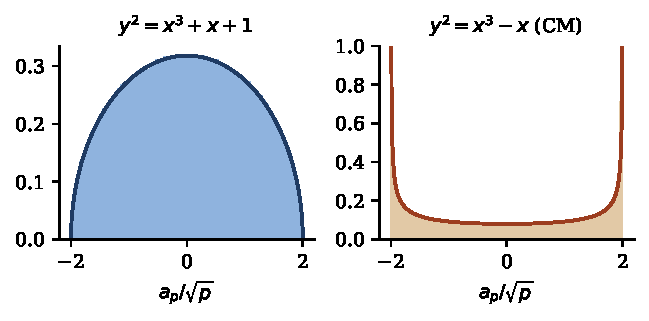
\includegraphics[width=\textwidth]{figs/satotate.pdf}
\caption{Normalised Frobenius traces $a_p/\sqrt p$ for all good primes below $10^7$. Left: $E_1:y^2=x^3+x+1$, histogram of all traces against the Sato Tate density $\sqrt{4-x^2}/(2\pi)$. Right: $E_2:y^2=x^3-x$, which has complex multiplication; histogram of the nonzero traces (the primes $p\equiv1\bmod4$), scaled to their share of all good primes (about $\tfrac12$), against the continuous part $1/(2\pi\sqrt{4-x^2})$ of $\mu_{\mathrm{CM}}$, which has mass $\tfrac12$. The atom of mass $\tfrac12$ at zero, from the primes $p\equiv3\bmod4$, is not drawn.}\label{fig:satotate}
\end{figure}

The two histograms distinguish two compact groups: the Sato Tate group of $E_1$ is $\SU(2)$, and that of $E_2$ is the normaliser $N(\mathrm{U}(1))$ of the diagonal torus. Telling them apart from data is a statistical problem, the subject of Chapter~\ref{ch:12}.

\section{A map of methods}

Table~\ref{tab:01map} lists the main families of probabilistic and computational methods that touch the programme, the target in each case, and what each delivers. ``Proves'' means the method is the engine of a theorem, usually with arithmetic input supplied from elsewhere. ``Reformulates'' means it recasts a conjecture as an equivalent probabilistic statement. ``Tests'' means it produces evidence, calibration or conjectural constants. ``None known'' means that no contribution is known.

\begin{table}[t]
\centering\small
\begin{tabular}{p{1.4in}p{1.4in}p{1.3in}}
\toprule
Method & Langlands target & Status\tabularnewline
\midrule
\raggedright Weyl criterion, moments & \raggedright Sato Tate and general Sato Tate laws & \raggedright proves, given functoriality\tabularnewline
\raggedright Tauberian theorems & \raggedright Prime number theorems for $L(s,\Sym^n\pi)$ & \raggedright proves, given automorphy\tabularnewline
\raggedright Random walks on trees & \raggedright $p$ adic Plancherel measure, Hecke operators & \raggedright proves\tabularnewline
\raggedright Trace formula as expectation & \raggedright Vertical Sato Tate \cite{serre1997,cdf1997} & \raggedright proves\tabularnewline
\raggedright Random walks on isogeny graphs & \raggedright Kemeny constants, spanning trees, mixing & \raggedright proves (Part~III and Chapter~\ref{ch:hit})\tabularnewline
\raggedright Random matrix theory & \raggedright Low lying zeros \cite{katzsarnak1999,ils2000} & \raggedright proves for restricted support (often under GRH), tests beyond\tabularnewline
\raggedright Interlacing, random graphs & \raggedright Bipartite Ramanujan graphs \cite{mss2015} & \raggedright proves\tabularnewline
\raggedright L\'evy and Thorin measures & \raggedright Positivity, Riemann hypothesis and Artin conjecture reformulations; squarefree integers (Chapter~\ref{ch:squarefree}); the steps of the proof of Fermat's last theorem (Chapter~\ref{ch:flt}); inversions between Frobenius traces, P\'olya kernels and zeros (Chapter~\ref{ch:lap}) & \raggedright reformulates, tests; proves identities (Chapters~\ref{ch:squarefree} and \ref{ch:lap})\tabularnewline
\raggedright Poisson Dirichlet law, Dirichlet processes & \raggedright Chebotarev densities in the prime factors of random integers, Mertens constants per class (Chapter~\ref{ch:pd}) & \raggedright proves\tabularnewline
\raggedright Extreme values & \raggedright $L$ values of eta products & \raggedright proves identities\tabularnewline
\raggedright Bayesian model choice & \raggedright Sato Tate group identification & \raggedright proves consistency, given equidistribution\tabularnewline
\raggedright Point counting, modular symbols & \raggedright Data for all of the above & \raggedright tests\tabularnewline
\raggedright Any of the above & \raggedright Reciprocity, functoriality & \raggedright no proof known\tabularnewline
\bottomrule
\end{tabular}
\caption{Probabilistic and computational methods in the Langlands programme, and what each delivers.}\label{tab:01map}
\end{table}

The last line of the table is the subject of the next section.

\section{The key limitation}\label{sec:01limits}

Could one prove reciprocity probabilistically, by showing that some sequence of Galois data has the statistics that automorphy forces? The following proposition shows that the limiting empirical law of the data cannot do it.

Let $\mathcal P$ be the set of primes. A set $S\subset\mathcal P$ has \emph{density zero} if $\#\{p\le x:p\in S\}/\pi(x)\to0$. Say that a sequence $(x_p)_{p\in\mathcal P}$ of real numbers \emph{comes from} a cuspidal automorphic representation $\pi$ of $\GL_2(\A)$ with trivial central character if $x_p=\tr A_p(\pi)$ for all but finitely many primes $p$, and call it \emph{automorphic} if it comes from some such $\pi$. Both notions are unchanged when finitely many terms are changed. A sequence $(x_p)\in[-2,2]^{\mathcal P}$ is equidistributed with respect to $\ST$ if $\pi(x)^{-1}\sum_{p\le x}\phi(x_p)\to\int\phi\,d\ST$ for every continuous $\phi$ on $[-2,2]$.

\begin{proposition}[Equidistribution does not determine automorphy; this book]\label{prop:01limits}\index{strong multiplicity one}
Let $\mathcal E$ be the set of sequences $(x_p)\in[-2,2]^{\mathcal P}$ that are equidistributed with respect to $\ST$.
\begin{enumerate}
\item $\mathcal E$ has the cardinality of the continuum and contains continuum many sequences no two of which agree at all but finitely many primes. The automorphic sequences fall into countably many classes under the relation of agreeing at all but finitely many primes, so all but countably many of those sequences are not automorphic.
\item Let $(x_p)\in[-2,2]^{\mathcal P}$ come from $\pi$, and let $(x'_p)\in[-2,2]^{\mathcal P}$ differ from $(x_p)$ exactly on an infinite set $S$ of density zero. Then $(x'_p)$ is not automorphic, and $(x'_p)\in\mathcal E$ if and only if $(x_p)\in\mathcal E$.
\end{enumerate}
\end{proposition}

\begin{proof}
We first show that density zero alterations do not change limits of empirical averages. Let $(x_p),(x'_p)\in[-2,2]^{\mathcal P}$ agree outside a density zero set $S$, and let $\phi$ be continuous on $[-2,2]$. Then
\[
\Bigl|\frac1{\pi(x)}\sum_{p\le x}\phi(x'_p)-\frac1{\pi(x)}\sum_{p\le x}\phi(x_p)\Bigr|\le 2\|\phi\|_\infty\,\frac{\#\{p\le x:p\in S\}}{\pi(x)}\longrightarrow0,
\]
so either both empirical averages converge, to the same limit, or neither does. In particular $(x'_p)\in\mathcal E$ if and only if $(x_p)\in\mathcal E$.

(1) By Theorem~\ref{thm:01satotate} the normalised eigenvalues $x_p=\tau(p)/p^{11/2}$ of $\Delta$ form an element of $\mathcal E$. Let $S$ be an infinite set of density zero, for instance $S=\{p_{k^2}:k\ge1\}$, where $p_j$ is the $j$th prime; it has $\lfloor\pi(x)^{1/2}\rfloor$ elements up to $x$. For $c\in[-2,2]$ let $(x^{(c)}_p)$ equal $c$ on $S$ and agree with $(x_p)$ off $S$. By the first paragraph each $(x^{(c)}_p)$ lies in $\mathcal E$, and for $c\ne c'$ the sequences $(x^{(c)}_p)$ and $(x^{(c')}_p)$ differ at every prime of the infinite set $S$. These are continuum many elements of $\mathcal E$, no two agreeing at all but finitely many primes, and $|\mathcal E|\le|[-2,2]^{\mathcal P}|=2^{\aleph_0}$.

On the other side, every cuspidal automorphic representation $\pi$ of $\GL_2(\A)$ has nonzero vectors fixed by some open compact subgroup $K$ of $\GL_2(\A_f)$. There are countably many such $K$, since each contains some principal congruence subgroup $K(N)$, is a finite union of cosets of $K(N)$, and $\GL_2(\A_f)/K(N)$ is countable. For fixed $K$, the cuspidal functions on $\GL_2(\Q)Z(\A)\backslash\GL_2(\A)$ that are right invariant under $K$ form a separable Hilbert space on which $\GL_2(\R)$ and the Hecke operators of level $K$ act with discrete spectrum and finite multiplicities, and each $\pi$ with trivial central character and nonzero $K$ fixed vectors occurs in it; so there are countably many such $\pi$. Hence there are countably many $\pi$ in all, and the sequences that come from a given $\pi$ form a single class under agreement at all but finitely many primes. A class contains at most one of the sequences $(x^{(c)}_p)$, so all but countably many of them are not automorphic.

(2) The second assertion was proved in the first paragraph. Suppose $(x'_p)$ came from some $\pi'$. Then $\tr A_p(\pi')=x'_p=x_p=\tr A_p(\pi)$ for all primes outside $S\cup F$, with $F$ finite, and $S\cup F$ has natural density zero, hence Dirichlet density zero. Ramakrishnan's refinement of strong multiplicity one \cite{ramakrishnan1994} states that two cuspidal automorphic representations of $\GL_2(\A)$ with trivial central character are isomorphic if their Hecke eigenvalues $\tr A_p$ agree at all primes outside a set of density less than $1/8$. Therefore $\pi'\cong\pi$, and hence $x'_p=\tr A_p(\pi)=x_p$ for all but finitely many $p$. This contradicts the hypothesis that the sequences differ at every prime of the infinite set $S$.
\end{proof}

\begin{corollary}[this book]\label{cor:01functional}
Let $\Phi$ be any function on $[-2,2]^{\mathcal P}$ that is unchanged when a sequence is altered on a set of density zero; for instance any function of the set of weak limit points of the empirical measures $\pi(x)^{-1}\sum_{p\le x}\delta_{x_p}$ as $x\to\infty$, which by the first paragraph of the proof above is unchanged by such alterations. Then for every automorphic $(x_p)\in[-2,2]^{\mathcal P}$ there are continuum many sequences in $[-2,2]^{\mathcal P}$ that are not automorphic and on which $\Phi$ takes the value it takes on $(x_p)$; if $(x_p)\in\mathcal E$, they all lie in $\mathcal E$. In particular $\Phi$ cannot characterise automorphy.
\end{corollary}

\begin{proof}
Fix an infinite set $S$ of density zero and apply part (2) of Proposition~\ref{prop:01limits} to every $(x'_p)\in[-2,2]^{\mathcal P}$ that agrees with $(x_p)$ off $S$ and differs from it at every prime of $S$. There are continuum many such sequences, since each $x'_p$ with $p\in S$ ranges over $[-2,2]\setminus\{x_p\}$; none is automorphic, and $\Phi$ takes the same value on all of them and on $(x_p)$.
\end{proof}

Any argument that uses only the limiting distribution of Frobenius traces therefore sees the same object for an automorphic representation and for continuum many nonautomorphic impostors. Rates of convergence do not help either. If $\epsilon(x)\pi(x)\to\infty$, there is an infinite set $S$ with $\#\{p\le x:p\in S\}\le\epsilon(x)\pi(x)$ for all $x$, and an alteration on $S$ changes every empirical average $\pi(x)^{-1}\sum_{p\le x}\phi(x_p)$ by at most $2\|\phi\|_\infty\epsilon(x)$. With $\epsilon(x)=\pi(x)^{-3/4}$, for instance, which satisfies both $\epsilon(x)\pi(x)\to\infty$ and $\epsilon(x)=o(\pi(x)^{-1/2})$, this gives impostors that the discrepancy statistics of Chapter~\ref{ch:05}, which live at the scale $\pi(x)^{-1/2}$, cannot see. What distinguishes the genuine sequence is structure that couples different primes: the analytic continuation and functional equation of the Dirichlet series built from it and of all its twists, and the Galois representation attached to it, which for an elliptic curve makes each $a_p=\sqrt p\,x_p$ an integer whose residue modulo a prime $\ell\ne p$ is determined by the Frobenius class of $p$ in the field generated by the $\ell$ torsion points. Converse theorems, from Weil \cite{weil1967} to Cogdell and Piatetski Shapiro \cite{cogdellps1994}, characterise automorphy through the first kind of coupling; modularity lifting theorems, from Wiles onward \cite{wiles1995,taylorwiles1995}, establish it through the second, by Galois deformation theory and congruences between automorphic forms. No probabilistic method currently exploits either. Chapter~\ref{ch:recip} restates part of the first kind of coupling as a symmetry of functions computed from Frobenius traces, the conductor and the gamma factor, and that part together with the generalized Riemann hypothesis as a positivity property of such functions; this is a reformulation, not a method of proof. Probability therefore enters the programme through consequences of the conjectures, as a calibration tool and as a source of reformulations, not as a proof technique for reciprocity itself.

\begin{remark}
The same argument applies to any statistic that is a limit of averages over primes in which each prime carries weight $O(1/\pi(x))$, for instance the empirical joint law of consecutive traces $(x_{p_n},x_{p_{n+1}})$. It says nothing about statistics that weight individual primes heavily, or that use the analytic properties of the full Dirichlet series and its twists. A sparser alteration, on an infinite set $S$ with $\sum_{p\in S,\,p\le x}\log p=o(\sqrt x)$, moves every twisted sum $\sum_{p\le x}x_p\chi(p)\log p$ by $o(\sqrt x)$, so properties of these sums at the square root scale cannot characterise automorphy either; whether, uniformly over characters $\chi$ of growing conductor, they can decide closeness to a newform is Open Problem~\ref{op:inverse} of Chapter~\ref{ch:13}.
\end{remark}

\section{What the methods deliver}

Within these limits there is a great deal to prove. The book is organised in five parts.

\subsection{Part I: Foundations}
Chapter~\ref{ch:02} develops modular forms, Hecke operators, Euler products and functional equations for readers trained in probability, and isolates two facts used throughout: normalised Hecke eigenvalues are traces of elements of $\SU(2)$, and the completed $L$ function of $\Delta$ is the Mellin transform of a positive function. Chapter~\ref{ch:03} treats Galois representations and the Chebotarev density theorem, reciprocity, the dual group and the Satake isomorphism, functoriality and the Sato Tate group, and records which cases are known. Appendix~\ref{app:A} collects the probability used later.

\subsection{Part II: Equidistribution}
The Weyl criterion on compact groups turns equidistribution into the vanishing of averages of characters. For $\SU(2)$ these are Chebyshev polynomials, and for the CM law $\mu_{\mathrm{CM}}$ the averages $\int U_n(x/2)\,d\mu_{\mathrm{CM}}$ equal $1$ when $4\mid n$ and $0$ otherwise, a fingerprint of the Sato Tate group. Chapter~\ref{ch:04} gives Serre's derivation of Sato Tate from symmetric power functoriality. Chapter~\ref{ch:05} studies the rate of convergence (the discrepancy $D_n$ of the first $n$ traces, which for our curves sits at the scale $n^{-1/2}$ of independent sampling), the bias of the weighted sums $\sum_{p\le x}a_p\log p/p$, which through the explicit formula and under the Riemann hypothesis for $L(s,E)$ encodes the analytic rank of an elliptic curve in logarithmic mean, and the Lang Trotter conjecture on how often $a_p$ takes a fixed value.

Chapter~\ref{ch:06} turns to the other random matrix limit, in which the dimension of the group tends to infinity and eigenvalues model zeros of $L$ functions: the pair correlation of Montgomery and Dyson, the symmetry types of Katz and Sarnak, low lying zeros of families of modular forms and the moment conjectures of Keating and Snaith. Chapter~\ref{ch:06b} finds the same semicircle in Kloosterman sums, through Katz's vertical Sato Tate theorem \cite{katz1988} and the random Fourier series of Kowalski and Sawin \cite{kowalskisawin2016}. Chapter~\ref{ch:06c} replaces Haar random elements of a compact group by random finite abelian groups: the Cohen Lenstra heuristics for class groups and the Poonen Rains model for Selmer groups, with what they predict for ranks, compared with class groups and Selmer groups computed for this book.

\subsection{Part III: Random walks and hitting times}
Hecke operators, suitably normalised, are Markov operators. The Bruhat Tits tree of the group $\PGL_2(\Q_q)$ is the $(q+1)$ regular tree, $T_q$ acts as its adjacency operator, and the spectral measure of simple random walk on the tree is the Kesten McKay law \cite{kesten1959,mckay1981}, which is also the $q$ adic Plancherel measure. Chapter~\ref{ch:07} shows that its Chebyshev moments are $q^{-n/2}$ for even $n$ and $0$ for odd $n$, and that it converges to the semicircle as $q\to\infty$, which explains heuristically, but does not prove, why the horizontal Sato Tate law (one form, the prime varying) and the vertical one (one prime, the form varying) are compatible. Chapter~\ref{ch:08} turns to finite quotients, whose Ihara zeta functions make the Ramanujan property a graph Riemann hypothesis, and to the supersingular isogeny graphs of Pizer \cite{pizer1990}, on which the Ramanujan bound for Hecke eigenvalues of weight two forms becomes an optimal spectral gap. We prove that the Kemeny constant of the supersingular $\ell$ isogeny graph, the expected time to hit a target drawn from the stationary distribution, is asymptotic to $\ell/(\ell-1)$ times the number of vertices.

\subsection{Part IV: L\'evy and Thorin measures}
Chapter~\ref{ch:09} starts from Khinchine's observation that for $\sigma>1$ the function $t\mapsto\zeta(\sigma+it)/\zeta(\sigma)$ is the characteristic function of an infinitely divisible law. For an automorphic $L$ function the corresponding L\'evy Khintchine exponent has weights of both signs, and positivity returns for Rankin Selberg $L$ functions: for $\sigma>1$, $t\mapsto L(\sigma+it,\pi\times\tilde\pi)/L(\sigma,\pi\times\tilde\pi)$ is again the characteristic function of an infinitely divisible law. Chapter~\ref{ch:09b} follows $\log|L|$ on the critical line, through Selberg's central limit theorem, the log correlated field of Fyodorov, Hiary and Keating and its maximum, and multiplicative chaos, tested on $L(s,\Delta)$.

For Ramanujan's $\Delta$ the completed $L$ function $\Lambda(s,\Delta)$ is the Mellin transform of the positive function $y\mapsto\Delta(iy)$, so $\Lambda(6+it)/\Lambda(6)$ is the characteristic function of a symmetric random variable, and the Riemann hypothesis for $\Delta$ says that this characteristic function has only real zeros. In Chapter~\ref{ch:10} we prove that the Riemann hypothesis for $\Delta$ is equivalent to $s\mapsto\Lambda(6)/\Lambda(6+\sqrt s)$ being the Laplace transform of a generalized gamma convolution in the sense of Thorin and Bondesson \cite{thorin1977,bondesson1992}, with Thorin measure carried by the squared ordinates of the zeros. This is a reformulation, not a proof. Chapters~\ref{ch:10b} and \ref{ch:10c}, extending the first author's earlier work \cite{polson2018vdp}, turn it into a framework. For every cuspidal automorphic representation of $\GL_n$ over $\Q$ the generalized Riemann hypothesis is equivalent to the Thorin property, to complete monotonicity of a L\'evy function built from the zeros, and to positive semidefiniteness of Hankel matrices of power sums computable from the central Taylor coefficients alone; the order of vanishing at the centre, which for an elliptic curve is the Mordell Weil rank under the conjecture of Birch and Swinnerton Dyer, appears as a degenerate Thorin atom at the origin of mass half the order. Locally the Ramanujan conjecture at a prime is exactly a Thorin property of the Euler factor, and the framework becomes unconditional for curves over finite fields, for Ramanujan graphs, including the supersingular isogeny graphs, and for Hecke random walks on Bruhat Tits trees, whose passage times are generalized gamma convolutions with explicit large deviations. Chapter~\ref{ch:10d} recasts all of this, as in \cite{polson2018vdp}, as van Dantzig pairs and Wald couples, proves the sine squared transport from Euler products to Thorin densities, and tests the class of Konstantopoulos, Patie and Sarkar \cite{konstantopoulospatiesarkar2024} against $L$ functions.

Chapters~\ref{ch:squarefree} to \ref{ch:scholze} test the framework on three cases. Chapter~\ref{ch:squarefree} follows the squarefree integers: their counting error is governed by the zeros of $\zeta$, the constant of the squarefree problem is a combination of two tilted means of the P\'olya law of $\xi$, a Gamma smoothing turns the error into an average of the Mertens function, and the Thorin picture extends into the critical strip and to imaginary quadratic fields, whose P\'olya kernels are positive when $|d|<\pi^2$ and take negative values whenever $2$ and $3$ are inert. Chapter~\ref{ch:beta} does the same for Dirichlet's $\beta$ function, whose kernel is built from the cube of Dedekind's eta function, and proves for $\beta$ and for $\xi$, on the lines $\operatorname{Re}s=\alpha$ with $\frac12<\alpha\le3.15$ and up to the heights to which their Riemann hypotheses are verified, that the real part of the logarithmic derivative is smallest on the real axis, which for $\xi$ Lagarias proved on every line to the right of the centre under the Riemann hypothesis, and Garunk\v{s}tis unconditionally for $\alpha\ge1$. Chapter~\ref{ch:scholze} computes signed Thorin densities by Stieltjes inversion and counts zeros numerically by the argument principle for $\zeta$, $L(s,\chi_{12})$ and $L(s,\Delta)$; its first section says where Scholze's work enters the theory of $L$ functions, and that the computations do not use it. None of the three chapters proves a Riemann hypothesis.

Chapter~\ref{ch:recip} turns these devices on reciprocity. It derives quadratic reciprocity and Gauss's sign from the characteristic function of the normal law, puts Frobenius traces and Hecke eigenvalues on one probability space, where irreducible Artin representations and cuspidal automorphic representations are both orthonormal systems of random variables, reads the Frobenius labelled prime factorisation of a random integer as a Gamma process, and restates Hecke's converse theorem at level one as a symmetry of a P\'olya kernel, and the holomorphy and the generalized Riemann hypothesis of a self dual Artin $L$ function as the complete monotonicity of a heat trace computed from Frobenius traces, the conductor and the gamma factor. These are reformulations. Finitely many evaluations of the heat trace can disprove holomorphy or the generalized Riemann hypothesis but are not known to verify them, even to a finite height, and no new case of reciprocity is proved.

Chapter~\ref{ch:hit} reads reciprocity through hitting times. For the walk on supersingular elliptic curves in characteristic $N$ along isogenies of degree $\ell$, the Kemeny constant is a harmonic sum of the factors $\ell+1-a_\ell(f)$ of $|J_0(N)(\mathbb F_\ell)|$, and for $N\equiv1\bmod12$ the number of spanning trees is $|J_0(N)(\mathbb F_\ell)|$ divided by the number of vertices, a formula of Hashimoto \cite{hashimoto1989,li2019} that Munier and Shnidman \cite{muniershnidman2023} read as a reciprocity law exchanging the two primes. Chebotarev densities become hitting rates for the largest prime factors of a random integer, the Thorin converse theorem a statement about explosion times of pure birth processes, and the functional equation of the $L$ function of an odd primitive Dirichlet character an identity between two expansions of a signed exit law of Brownian motion. These too are reformulations, and no new case of reciprocity is proved.

Chapter~\ref{ch:flt} follows the proof of Fermat's last theorem through the same language. Weight one newforms, through which the theorem of Langlands and Tunnell gives the residual modularity that Wiles's argument starts from, are exactly the newforms whose label laws are supported on finitely many points; modularity becomes, through Weil's converse theorem, a family of reflection symmetries of twisted P\'olya kernels built from point counts and the conductor; the density of the primes $\ell$ at which $p$ does not divide $|E(\mathbb F_\ell)|$, the local density of Koblitz's conjecture, becomes the shape of a Gamma law, positive for a Frey curve and $p\ge5$ by Serre's argument from Mazur's torsion theorem; and the genus zero of $X_0(2)$, which ends the proof, becomes the emptiness of a Thorin measure built from Hecke eigenvalues, or a Kemeny constant equal to zero. These are restatements: no step of the proof is reproved and no new case of modularity is proved, and the content of the proof is in the theorems of Langlands and Tunnell, Mazur, Ribet, Wiles, and Taylor and Wiles, on the curve of Hellegouarch and Frey and the reduction of Frey and Serre.

Chapter~\ref{ch:lap} collects the inverse Laplace transforms behind the earlier chapters of this part and computes with them. Bohr means invert the sine squared transport, so that the transported density of an $L$ function on any half line determines its Frobenius traces, which we recover at the primes below $64$ from the transported density of $\eta(z)\eta(23z)$. Bromwich inversion of the Artin $L$ function of $x^3-x-1$ on the critical line, computed as $\zeta_K/\zeta$, returns the weight one form; it uses the holomorphy of this $L$ function, which Hecke's identification of it with the $L$ function of the form supplies, and in general the modularity of the result is the content of Weil's converse theorem. As in \cite{polson2017}, the shifted Thorin densities of Chapter~\ref{ch:10d} form a Cauchy semigroup in the basepoint, in which each zero is seen through Cauchy noise, and by a theorem of Roynette and Yor \cite{roynetteyor2005} the Thorin variable of an Euler product with nonnegative coefficients has a Pareto tail of index $\frac32$. A last section relates atomic Thorin laws to the B splines of Curry and Schoenberg, and reads the Sato Tate law as the density that minimises the roughness penalty of Good and Gaskins among those vanishing on the walls of the alcove. Most of these results are known, and no case of reciprocity is proved.

Chapter~\ref{ch:pd} relates the Gamma process of Chapter~\ref{ch:recip} to classical laws. The normalised sizes of the prime factors of a uniform random integer follow the Poisson Dirichlet law by Billingsley's theorem, as the normalised cycle lengths of a random permutation do; normalised, the Gamma process with Frobenius labels is Ferguson's Dirichlet process, whose base measure is the Haar measure that Chebotarev's theorem gives, so that the limit of every Frobenius functional is a standard exponential variable times a Dirichlet mean; and the random integers weighted by the coefficients of the powers of $\zeta$ give the whole Ewens family, with the exponent of the singularity at $s=1$ as Ewens parameter. For a uniform random integer below $x$, the class of a size biased prime factor approaches Haar measure at rate $1/\log x$, the class of the largest one faster still, but the classes of the distinct prime factors only at rate $1/\log\log x$, with Mertens constants per class computed from $L(1,\chi)$ and $\frac{L'}L(1,\chi)$: among the distinct prime factors of random integers below $10^7$, the primes that split completely in the field of $x^3-x-1$ have less than half their Haar share. A last section asks which of Bondesson's theorems on generalized gamma convolutions do arithmetic work. These are theorems about random integers, most of them known, and no case of reciprocity is proved.

Chapter~\ref{ch:gl1} treats degree one, where reciprocity is a theorem: by Kronecker and Weber over $\Q$, by Artin's reciprocity law over a number field, and for Hecke's characters of infinite order. Dirichlet's theorem on primes in progressions becomes a Dirichlet process on the classes modulo $q$, with Mertens constants computed from $L(1,\chi)$ and with Landau's theorem on the integers that have no prime factor in a given class as the atom at zero of Chapter~\ref{ch:pd}; Hecke's theorem on the angles of Gaussian primes becomes a Dirichlet process on the circle; and the Thorin measure of a degree one $L$ function is checked against its zeros. By Deuring's theorem the $L$ function of an elliptic curve with complex multiplication is that of a Hecke character of the imaginary quadratic field, and seen from that field the Rankin Selberg subordinator of Chapter~\ref{ch:recip} is the sum of two independent copies of itself seen from $\Q$, so that the Gamma shape test of Chapter~\ref{ch:recip} detects complex multiplication, here as a theorem.

Chapter~\ref{ch:maass} turns to the Maass forms, the eigenfunctions of the hyperbolic Laplacian on the modular surface and the other half of the automorphic spectrum of $\SL_2(\Z)$. With the normalised hyperbolic area the modular surface is a probability space, and Brownian motion on it is ergodic with that law. Read as a heat trace, the Selberg trace formula of a compact hyperbolic surface says that the total return probability of Brownian motion is the free return probability plus a sum over closed geodesics, which is McKean's reading \cite{mckean1972}. Selberg's eigenvalue conjecture becomes the complete monotonicity of the heat trace over the cusp forms, as the holomorphy and the generalized Riemann hypothesis of a self dual Artin $L$ function became that of a heat trace in Chapter~\ref{ch:recip}. Weyl's law keeps the eigenvalues out of the Thorin class, while the closed geodesics, ordered by length, form a system of primes to which the sine squared transport of Chapter~\ref{ch:10d} and the Poisson Dirichlet limits of Chapter~\ref{ch:pd} apply unconditionally. A last section states the Eichler Selberg trace formula and reads it as the moment identity behind Serre's vertical Sato Tate law. These are reformulations, and no new case of Selberg's conjecture is proved.

Chapter~\ref{ch:percolation} takes up the other body of Langlands's work, on conformal invariance in critical percolation. Cardy's formula for the probability that a critical rectangle of aspect ratio $r$ is crossed from left to right is the distribution function of a $\mathrm{Beta}(\frac13,\frac13)$ law at the modular lambda function of $ir$, and the log odds of that law is an extended generalized gamma convolution with Thorin atoms at $n+\frac13$. Differentiating in $r$ gives a constant times $\eta(ir)^4$, so that the aspect ratio at which a critical rectangle stops being crossed is a random variable whose Mellin transform is, up to a constant, the completed $L$ function of the elliptic curve $y^2=x^3+1$ of conductor $36$: the modularity of the curve is what turns a percolation law into an $L$ function. The logarithm of this crossing threshold is not infinitely divisible and the threshold is not a generalized gamma convolution, but numerically it is infinitely divisible and self decomposable, the probabilistic form of the renormalisation fixed point of Langlands, Pouliot and Saint Aubin. The generalized Riemann hypothesis for the curve is equivalent to the positivity of Hankel matrices built from the cumulants of the logarithm of the threshold, and a Prony step on those cumulants recovers the first zero of the $L$ function to twelve digits. These are reformulations of a known case of reciprocity, and no Riemann hypothesis is proved.

Finally, in Chapter~\ref{ch:11}, the product $\prod_n(1-e^{-2\pi ny})$ is the distribution function of the maximum of independent exponentials $E_n/(2\pi n)$, which gives an extreme value representation of the $L$ functions of multiplicative eta products. For example, $L(E_{11a},1)=0.2538419\ldots$ is the probability that an independent standard exponential exceeds $2\pi M$, where $M$ is the maximum of independent variables $E/(2\pi n)$ and $E/(22\pi n)$, $n\ge1$, two of each, read off from the eta product $\eta(\tau)^2\eta(11\tau)^2$ of $E_{11a}$.

\subsection{Part V: Inference and open problems}
Chapter~\ref{ch:11b} treats Haar measure on locally compact groups. On a compact Sato Tate group left and right Haar measure coincide, but on the Borel subgroup that acts on the upper half plane they differ: hyperbolic area is left Haar measure, while right Haar measure is the prior whose invariant credible sets are exact confidence sets in a transformation model. We connect this to Barndorff Nielsen's $p^*$ formula, which is exact in such models, to the reference priors of Chang and Eaves for orbits, which bear on inference about Satake parameters as conjugacy classes, and to Duke's equidistribution of Heegner points for the invariant measure, which we check on $28{,}251$ points. Chapter~\ref{ch:12} asks which Sato Tate group a curve has, given its traces at the first $n$ primes. We prove that Bayes factors between candidate groups are consistent when the traces are equidistributed for the true law, atoms included, with exponential rates given by differences of Kullback Leibler divergences. In genus two we compare three candidate groups and study a curve whose group lies outside the candidate set. Chapters~\ref{ch:13} and \ref{ch:14} collect the open problems and the computational programme.

\section{How to read this book}

A reader comfortable with measure theoretic probability, characteristic functions and Markov chains, and with complex analysis at the level of Mellin transforms and the Gamma function, has the prerequisites for this book. Algebraic number theory and representation theory are used, but each chapter states the results it needs and gives references.

Conjectures are labelled as conjectures. Known theorems are attributed, and those with long proofs are stated with a sketch and a reference. Results that are new in this book, including Proposition~\ref{prop:01limits}, the Kemeny constant limit, the Bayesian consistency theorem, the Thorin criteria for the generalized Riemann hypothesis of automorphic $L$ functions and for the Ramanujan conjecture, the Thorin structure of Hecke passage times, and the extreme value representation, are identified as ours and are given complete proofs. Numerical values are from computations carried out for this book, mainly in PARI/GP and Python, and are reported to the precision we verified.

Every chapter except the last two ends with exercises and a short list of open computational problems. These are posed and not solved. Each specifies an objective, the objects and the data scale, a suggested software route, the expected deliverable, and the reason it matters. Together they form a programme of computational experiments, collected and prioritised in Chapter~\ref{ch:14}. Their purpose is to measure the probabilistic shadow at scales where the predictions become sharp, and to look for rates, biases or constants that depart from what the theory predicts.

\section{Notes}

Langlands' letter to Weil \cite{langlands1967} and his 1970 lectures \cite{langlands1970} remain the best primary sources for the original vision. Gelbart's survey \cite{gelbart1984} is the standard introduction, Arthur \cite{arthur2003} explains functoriality, and Frenkel \cite{frenkel2007} gives the geometric side. The naming of the modularity conjecture for elliptic curves has been disputed; Lang \cite{lang1995} collects the documents. Serre's book on $\ell$ adic representations \cite{serre1968} contains the derivation of Sato Tate from analytic properties of symmetric power $L$ functions, and Tate's paper \cite{tate1965} records the conjecture from the side of algebraic cycles. Strong multiplicity one for $\GL_n$ is due to Jacquet and Shalika \cite{jacquetshalika1981}. The refinement for $\GL_2$ that we use is Ramakrishnan's \cite{ramakrishnan1994}, and an example of Serre built from dihedral forms shows that its threshold $1/8$ for the density of the exceptional set cannot be raised. Katz and Sarnak \cite{katzsarnak1999,katzsarnak1999b} developed the random matrix side of the shadow, the subject of Chapter~\ref{ch:06}. The point of view that probability sees the consequences of functoriality rather than functoriality itself is implicit in much of this literature; Proposition~\ref{prop:01limits} makes one version of it precise, and given Ramakrishnan's theorem its proof is elementary.

\section{Exercises}

\begin{enumerate}
\item Show that the even moments of $\ST$ are the Catalan numbers $\frac1{m+1}\binom{2m}{m}$ and that its odd moments vanish.
\item Let $\theta$ have density $\frac2\pi\sin^2\theta$ on $[0,\pi]$. Show that $2\cos\theta$ has law $\ST$, and that $\E[U_n(\cos\theta)]=0$ for every $n\ge1$, where $U_n(\cos\theta)=\sin((n+1)\theta)/\sin\theta$.
\item Show that the set of primes $\{p_{k^2}:k\ge1\}$ has density zero, where $p_j$ is the $j$th prime. Show that density zero cannot be weakened to positive upper density in Proposition~\ref{prop:01limits}: for every set $S$ of primes of positive upper density, construct an alteration on $S$ of an $\ST$ equidistributed sequence that is not $\ST$ equidistributed.
\item Let $(x_p)$ come from a newform $f$ of weight $k\ge2$ with trivial character and without complex multiplication, and let $(x'_p)$ be obtained by replacing $x_p$ by $-x_p$ for $p$ in a set $S$ of density $\delta$. Show that if $\delta<1/8$ and $x_p\neq0$ for infinitely many $p\in S$, then $(x'_p)$ is not automorphic. Now let $S$ be the set of primes $p$ with $\left(\frac p5\right)=-1$, of density $\tfrac12$. Show that $(x'_p)$ comes from the twist of $f$ by the quadratic character modulo $5$, and is therefore automorphic and $\ST$ equidistributed. Why does this not contradict Proposition~\ref{prop:01limits}?
\item Let $\nu(dx)=dx/(\pi\sqrt{4-x^2})$ be the arcsine law on $[-2,2]$, the continuous part of $\mu_{\mathrm{CM}}$ normalised to mass one. Compute the Kullback Leibler divergence $\int\log\frac{d\nu}{d\ST}\,d\nu$, using $\int_0^\pi\log\sin\theta\,d\theta=-\pi\log2$. Interpret the answer as the rate at which a likelihood ratio test tells a CM curve from a generic one using only the traces at the split primes.
\item Let $\chi$ be a nontrivial Dirichlet character modulo $N$. Using the prime number theorem for arithmetic progressions, show that, as $p$ runs over the primes not dividing $N$, the values $\chi(p)$ are equidistributed with respect to the uniform measure on the image $\chi((\Z/N\Z)^\times)$, a finite cyclic group of roots of unity, and explain why this is the case $n=1$ of the probabilistic shadow.
\end{enumerate}

\section{Open computational problems}

\begin{compproblem}[A Sato Tate atlas for elliptic curves]
Objective: compute and publish the empirical Sato Tate law, the Weyl averages $\pi(x)^{-1}\sum_{p\le x}U_k(x_p/2)$ for $k\le30$, and the normalised Kolmogorov discrepancy $\sqrt n\,D_n$ of the first $n$ traces, for every isogeny class of elliptic curves over $\Q$ of conductor up to $10^5$ in the LMFDB \cite{lmfdb}, using all good primes below $10^9$. Route: Sutherland's \texttt{smalljac} library or PARI/GP \texttt{ellap}, distributed over a cluster; the traces depend only on the isogeny class, so store results by class. Deliverable: a public table, and a plot of the Weyl averages against $k$ for each of the two Sato Tate groups that occur, $\SU(2)$ and $N(\mathrm{U}(1))$. Why it matters: it gives the empirical baseline against which every rate in Part~II is calibrated, and it would detect any curve whose Weyl averages decay anomalously slowly.
\end{compproblem}

\begin{compproblem}[Detecting impostors]
Objective: to quantify Proposition~\ref{prop:01limits} in data. Take the traces of $E_1$ for primes below $10^8$ and construct impostor sequences by replacing them, on density zero sets of increasing size (the primes $p_{k^2}$, the primes $p_{\lfloor k^{3/2}\rfloor}$, and random sets of $x^{\beta}$ primes up to $x$ for $\beta<1$), by independent draws from $\ST$. For each impostor compute (a) distributional statistics, such as the scaled discrepancy $\sqrt n\,D_n$ of the first $n$ traces against $\ST$ and the Weyl averages, whose limits cannot separate impostor from genuine sequence; and (b) coupling statistics, such as the defect of the functional equation of the Dirichlet series obtained by propagating the altered traces multiplicatively, evaluated on the critical line at heights up to about $2\pi x/\sqrt{496}$, so that coefficients up to $x$ carry weight, and Hecke consistency checks at prime squares when the traces at $p^2$ are included. Route: PARI/GP \texttt{lfuncreate} with user supplied coefficients and \texttt{lfuncheckfeq} at low height, and a smoothed approximate functional equation in C or Python at large height. Deliverable: power curves for each test as a function of the alteration size and the number of primes used. Why it matters: it measures how quickly coupling statistics see what distributional statistics cannot, and it is a first experiment towards the probabilistic converse theorem of Open Problem~\ref{op:inverse}.
\end{compproblem}

\begin{compproblem}[Near coincidences of newforms]
Objective: for all pairs of weight two newforms with rational coefficients and level up to $10^4$, compute the proportion of primes below $10^6$ at which their Hecke eigenvalues agree, and find the pairs with the largest such proportion. Route: LMFDB downloads or Sage modular symbols, with locality sensitive hashing on random sets of primes (two forms that agree at a proportion $\alpha$ of primes collide on $k$ sampled primes with probability about $\alpha^k$) to avoid comparing all pairs. Deliverable: a table of the most nearly coincident pairs, each explained where possible (quadratic twists, for instance, agree at the primes where the twisting character equals one and at the supersingular primes), and a histogram of agreement proportions, compared with the threshold $7/8$ of Ramakrishnan. Why it matters: it shows how far the threshold of strong multiplicity one is from the agreement actually seen between distinct forms, and so how many primes a certificate of equality based on agreement of traces needs in practice.
\end{compproblem}

\chapter{Modular Forms and L Functions for Probabilists}\label{ch:02}

In 1916 Srinivasa Ramanujan published a paper on certain arithmetical functions \cite{ramanujan1916} in which he studied the coefficients $\tau(n)$ of the power series $q\prod_{n\ge1}(1-q^n)^{24}$. From a table of thirty values he guessed three properties: $\tau$ is multiplicative, it satisfies a second order recursion at prime powers, and $|\tau(p)|\le2p^{11/2}$. Mordell proved the first two a year later \cite{mordell1917}; the third waited until Deligne's proof of the Weil conjectures in 1974 \cite{deligne1974}. Hecke's theory of operators on modular forms explains the first two observations, and the third is the prototype of the Ramanujan conjecture for automorphic representations. This chapter develops the objects of that story for readers whose training is in probability: modular forms, Hecke operators, Euler products, Mellin transforms and functional equations. Along the way we isolate two facts that drive the later parts of the book: by Deligne's theorem the normalised Hecke eigenvalues are traces of elements of $\SU(2)$, and the completed $L$ function of $\Delta$ is the Mellin transform of a \emph{positive} function.

\section{The modular group and modular forms}\label{sec:02forms}

The group $\SL_2(\Z)$ of integer matrices of determinant one acts on the upper half plane $\mathbb H=\{\tau\in\C:\Im\tau>0\}$ by M\"obius transformations
\[
\gamma\tau=\frac{a\tau+b}{c\tau+d},\qquad\gamma=\begin{pmatrix}a&b\\c&d\end{pmatrix}\in\SL_2(\Z),
\]
and $\Im(\gamma\tau)=\Im\tau/|c\tau+d|^2$. The group is generated by the matrices $T$ and $S$ that act by $\tau\mapsto\tau+1$ and $\tau\mapsto-1/\tau$, and every orbit meets the closed fundamental domain $\mathcal F=\{\tau\in\mathbb H:|\Re\tau|\le\tfrac12,\ |\tau|\ge1\}$. The quotient $\SL_2(\Z)\backslash\mathbb H$ has finite hyperbolic area $\pi/3$ for the measure $dx\,dy/y^2$, where $\tau=x+iy$, so $\frac3\pi\,dx\,dy/y^2$ is a probability measure on it; it is the limit law of Heegner points in Chapter~\ref{ch:11b}.

\begin{definition}\index{modular form}
Let $k$ be an even integer. A \emph{modular form} of weight $k$ for $\SL_2(\Z)$ is a holomorphic function $f$ on $\mathbb H$ with
\[
f(\gamma\tau)=(c\tau+d)^kf(\tau)\qquad\text{for all }\gamma\in\SL_2(\Z),
\]
which is holomorphic at infinity in the following sense. Invariance under $T$ gives a Fourier expansion $f(\tau)=\sum_{n\in\Z}a(n)q^n$ in $q=e^{2\pi i\tau}$, and we require $a(n)=0$ for $n<0$. If also $a(0)=0$, $f$ is a \emph{cusp form}. The spaces are $M_k$ and $S_k$.
\end{definition}

Invariance under $S$ is the nontrivial condition: $f(-1/\tau)=\tau^kf(\tau)$. The spaces are finite dimensional: for even $k\ge0$, $\dim M_k=\lfloor k/12\rfloor+1$ unless $k\equiv2\bmod12$, in which case $\dim M_k=\lfloor k/12\rfloor$, and $\dim S_k=\dim M_k-1$ for $k\ge4$ \cite{serre1973}. In particular $S_k=0$ for $k<12$ and for $k=14$, and $\dim S_{12}=1$.

\subsection{Eisenstein series}
\index{Eisenstein series}
For even $k\ge4$ the series $\sum_{(c,d)\neq(0,0)}(c\tau+d)^{-k}$ converges absolutely and is visibly of weight $k$. Normalised to have constant term one it becomes
\[
E_k(\tau)=1-\frac{2k}{B_k}\sum_{n\ge1}\sigma_{k-1}(n)q^n,\qquad\sigma_{k-1}(n)=\sum_{d\mid n}d^{k-1},
\]
with $B_k$ the Bernoulli numbers. Thus $E_4=1+240\sum\sigma_3(n)q^n$ and $E_6=1-504\sum\sigma_5(n)q^n$. The coefficients $\sigma_{k-1}(n)$ are multiplicative, and at a prime $\sigma_{k-1}(p)=1+p^{k-1}$. This is the degenerate case of everything that follows. The form $E_k$ is an eigenvector of the Hecke operator $T_p$ of the next section with eigenvalue $\sigma_{k-1}(p)$; the roots of $X^2-\sigma_{k-1}(p)X+p^{k-1}$ are $1$ and $p^{k-1}$, and after division by $p^{(k-1)/2}$ they are $p^{\pm(k-1)/2}$, far from the unit circle. The normalised eigenvalues $p^{(k-1)/2}+p^{-(k-1)/2}$ are unbounded, so they are not traces of elements of a compact subgroup of $\GL_2(\C)$: equidistribution in a compact group, the probabilistic shadow of Chapter~\ref{ch:01}, is a phenomenon of cusp forms.

\subsection{Ramanujan's Delta}
\index{Ramanujan Delta function}
The normalised cusp form of weight $12$ is
\[
\Delta(\tau)=\frac{E_4(\tau)^3-E_6(\tau)^2}{1728}=q\prod_{n\ge1}(1-q^n)^{24}=\sum_{n\ge1}\tau(n)q^n=\eta(\tau)^{24},
\]
where $\eta(\tau)=q^{1/24}\prod_n(1-q^n)$ is the Dedekind eta function\index{Dedekind eta function}. The equality of the Eisenstein expression with the product is Jacobi's; it can be proved by checking that the product is a cusp form of weight $12$, using the transformation law $\eta(-1/\tau)=\sqrt{\tau/i}\,\eta(\tau)$, and comparing the first coefficient.

\begin{example}\label{ex:02tau}
Expanding $q(1-q)^{24}(1-q^2)^{24}(1-q^3)^{24}\cdots$ to order $q^4$: the coefficient of $q^2$ comes only from $(1-q)^{24}$ and is $\tau(2)=-24$. The coefficient of $q^3$ receives $\binom{24}{2}=276$ from $(1-q)^{24}$ and $-24$ from $(1-q^2)^{24}$, so $\tau(3)=252$. For $q^4$ we collect $-\binom{24}{3}=-2024$ from $q^3$ in $(1-q)^{24}$, then $(-24)\cdot(-24)=576$ from $q\cdot q^2$, and $-24$ from $q^3$ in $(1-q^3)^{24}$, so $\tau(4)=-2024+576-24=-1472$. Continuing, $\tau(5)=4830$ and $\tau(6)=-6048=\tau(2)\tau(3)$.
\end{example}

\begin{theorem}[Ramanujan's observations]\label{thm:02ramanujan}
The coefficients $\tau(n)$ satisfy:
\begin{enumerate}
\item $\tau(mn)=\tau(m)\tau(n)$ when $\gcd(m,n)=1$ (Mordell, 1917);
\item $\tau(p^{r+1})=\tau(p)\tau(p^r)-p^{11}\tau(p^{r-1})$ for primes $p$ and $r\ge1$ (Mordell, 1917);
\item $|\tau(p)|\le2p^{11/2}$ for all primes $p$ (Deligne \cite{deligne1974}).
\end{enumerate}
\end{theorem}

The first two follow from the theory of Hecke operators in the next section, since $\Delta$ spans the one dimensional space $S_{12}$. The third follows from the Weil conjectures, which Deligne proved, applied to a Kuga Sato variety: a smooth compactification of the tenth fibre power of the universal elliptic curve (with auxiliary level structure), a variety of dimension $11$ in whose cohomology $\tau(p)$ is the trace of Frobenius on a two dimensional piece of $H^{11}$ \cite{deligne1971}. Example~\ref{ex:02tau} checks (2) at $p=2$, $r=1$: $\tau(2)^2-2^{11}=576-2048=-1472=\tau(4)$.

Whether $\tau(n)$ is ever zero is a question Lehmer raised in 1947 \cite{lehmer1947}, still open. Lehmer showed that the least $n$ with $\tau(n)=0$, if any, is prime; computations of Derickx, van Hoeij and Zeng \cite{derickx2013} based on congruences for $\tau$ have shown that $\tau(n)\neq0$ for all $n$ below $8\times10^{23}$. Serre proved that the primes with $\tau(p)=0$ have density zero \cite{serre1981}. Lehmer's question is the weight $12$ analogue of the Lang Trotter question for the trace $t=0$ (Chapter~\ref{ch:05}). If $\tau(p)/p^{11/2}$ behaved like an independent draw from the Sato Tate law of Chapter~\ref{ch:01}, rounded to the lattice $p^{-11/2}\Z$, the event $\tau(p)=0$ would have probability of order $p^{-11/2}$, a summable sequence. The same heuristic gives probability of order $p^{-1/2}$ for $a_p=0$ on an elliptic curve and so predicts infinitely many supersingular primes; for $\Delta$ it predicts only finitely many zeros of $\tau(p)$, and probably none.

\section{Hecke operators}
\index{Hecke operator}
For a prime $p$ the Hecke operator $T_p$ on $M_k$ sums $f$, viewed as a function of lattices, over the $p+1$ sublattices of index $p$. In coordinates,
\[
(T_pf)(\tau)=p^{k-1}f(p\tau)+\frac1p\sum_{j=0}^{p-1}f\Bigl(\frac{\tau+j}{p}\Bigr),
\]
and on $q$ expansions
\[
a(T_pf,n)=a(np)+p^{k-1}a(n/p),
\]
where $a(n/p)=0$ if $p\nmid n$. The operators $T_n$ for all $n\ge1$ are defined similarly by summing over sublattices of index $n$, and satisfy:

\begin{proposition}[Hecke relations]\label{prop:02hecke}
The operators $T_n$ commute, $T_{mn}=T_mT_n$ for coprime $m,n$, and for each prime $p$ and $r\ge1$,
\[
T_pT_{p^r}=T_{p^{r+1}}+p^{k-1}T_{p^{r-1}}.
\]
\end{proposition}

\begin{proof}[Proof sketch]
Identify $f$ with the function $F(\Z\omega_1+\Z\omega_2)=\omega_2^{-k}f(\omega_1/\omega_2)$ of lattices, where $\Im(\omega_1/\omega_2)>0$; it satisfies $F(\lambda L)=\lambda^{-k}F(L)$, and $T_n$ becomes $T_nF(L)=n^{k-1}\sum_{[L:L']=n}F(L')$. Coprime indices factor uniquely through intermediate lattices, which gives multiplicativity. For the prime power relation, count pairs $L''\subset L'\subset L$ with $[L:L']=p$ and $[L':L'']=p^r$: each sublattice $L''$ of index $p^{r+1}$ arises once unless $L''\subset pL$, in which case it arises $p+1$ times. The excess $p$ copies of each sublattice of $pL$ of index $p^{r-1}$ in $pL$ give the term $p^{k-1}T_{p^{r-1}}$ after the weight normalisation, since $F(pL)=p^{-k}F(L)$. Commutativity follows, since each $T_n$ is then a polynomial in the $T_p$ with $p\mid n$, and $T_pT_q=T_{pq}=T_qT_p$ for primes $p\neq q$. Details are in \cite{serre1973}.
\end{proof}

The relation at a prime is a three term recursion, the same one satisfied by Chebyshev polynomials. If $f$ is a simultaneous eigenvector of all $T_n$ with $a(1)=1$, an \emph{eigenform}, then $a(n)$ is the eigenvalue of $T_n$ (compare the coefficients of $q$ on both sides of $T_nf=\lambda_nf$, using $a(T_nf,1)=a(n)$), and the Hecke relations become
\[
a(mn)=a(m)a(n)\quad(\gcd(m,n)=1),
\]
\[
a(p^{r+1})=a(p)a(p^r)-p^{k-1}a(p^{r-1}).
\]
Since $S_{12}$ is one dimensional, $\Delta$ is an eigenform and Theorem~\ref{thm:02ramanujan}(1),(2) follow.

\subsection{Euler products and Satake parameters}
\index{Satake parameter}
Let $f$ be an eigenform, put $x_p=a(p)/p^{(k-1)/2}$, and let $\alpha_p,\beta_p$ be the roots of $X^2-x_pX+1$, so that $a(p)=p^{(k-1)/2}(\alpha_p+\beta_p)$ and $\alpha_p\beta_p=1$. The recursion becomes
\[
\frac{a(p^r)}{p^{r(k-1)/2}}=\frac{\alpha_p^{r+1}-\beta_p^{r+1}}{\alpha_p-\beta_p}=U_r(x_p/2),
\]
by induction, since the Chebyshev polynomials $U_r$ of the second kind satisfy $U_{r+1}(x/2)=xU_r(x/2)-U_{r-1}(x/2)$; the middle term is read as $(r+1)\alpha_p^r$ when $\alpha_p=\beta_p$. Multiplicativity and the generating function $\sum_{r\ge0}U_r(x/2)t^r=(1-xt+t^2)^{-1}$ give, where the series converges absolutely (for $\Re s>k/2+1$ by Hecke's bound in Section~\ref{sec:02mellin}),
\begin{align*}
L(s,f)=\sum_{n\ge1}\frac{a(n)}{n^s}&=\prod_p\bigl(1-a(p)p^{-s}+p^{k-1-2s}\bigr)^{-1}\\
&=\prod_p\bigl(1-\alpha_pp^{\frac{k-1}2-s}\bigr)^{-1}\bigl(1-\beta_pp^{\frac{k-1}2-s}\bigr)^{-1},
\end{align*}
an Euler product of degree two. The pair $\{\alpha_p,\beta_p\}$ is the Satake parameter, the conjugacy class of $\mathrm{diag}(\alpha_p,\beta_p)$ in $\SL_2(\C)$. Since $a(p)$ is real ($T_p$ is self adjoint for the Petersson inner product of Section~\ref{sec:02level}), Deligne's bound $|a(p)|\le2p^{(k-1)/2}$ is equivalent to $|\alpha_p|=|\beta_p|=1$, that is, to $\alpha_p=e^{i\theta_p}$, $\beta_p=e^{-i\theta_p}$ with $\theta_p\in[0,\pi]$, and then
\[
x_p=\frac{a(p)}{p^{(k-1)/2}}=2\cos\theta_p\in[-2,2].
\]
In probabilistic language: the Satake parameter is a conjugacy class in $\SU(2)$, the normalised eigenvalue $x_p$ is its trace, and the normalised coefficient $a(p^r)/p^{r(k-1)/2}=U_r(x_p/2)$ is the character of $\Sym^r$ evaluated on it. The Sato Tate law, a theorem for $\Delta$ (Theorem~\ref{thm:01satotate}), says that the $\theta_p$ are equidistributed with respect to $\frac2\pi\sin^2\theta\,d\theta$ on $[0,\pi]$, the law of the angle of a Haar random element of $\SU(2)$; equivalently, the $x_p$ are equidistributed with respect to $\ST$.

Figure~\ref{fig:tau} shows this for $\Delta$ and the primes below $10^6$; Chapter~\ref{ch:05} measures the fit by moments (Table~\ref{tab:05moments}), extreme values and discrepancy.

\begin{figure}[t]
\centering
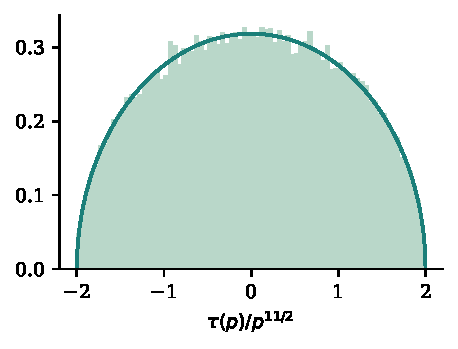
\includegraphics[width=\textwidth]{figs/tau.pdf}
\caption{Histogram of the normalised Ramanujan coefficients $x_p=\tau(p)/p^{11/2}$ for the $78{,}498$ primes $p<10^6$, against the Sato Tate density $\frac1{2\pi}\sqrt{4-x^2}$ on $[-2,2]$.}\label{fig:tau}
\end{figure}

\section{Mellin transforms and the functional equation}\label{sec:02mellin}
\index{Mellin transform}\index{functional equation}

The Mellin transform passes from modular forms to $L$ functions through the Gamma integral
\[
\int_0^\infty e^{-2\pi ny}y^{s-1}\,dy=(2\pi n)^{-s}\Gamma(s)\qquad(\Re s>0,\ n\ge1).
\]
Let $f=\sum a(n)q^n$ be a cusp form of weight $k$. The function $y^{k/2}|f(x+iy)|$ is invariant under $\SL_2(\Z)$ and bounded, since $f$ decays at the cusp, and $a(n)=e^{2\pi ny}\int_0^1f(x+iy)e^{-2\pi inx}\,dx$ for every $y>0$; the choice $y=1/n$ gives Hecke's bound $a(n)=O(n^{k/2})$. Hence $L(s,f)$ converges absolutely for $\Re s>k/2+1$, and on that half plane termwise integration gives
\[
\Lambda(s,f):=(2\pi)^{-s}\Gamma(s)L(s,f)=\int_0^\infty f(iy)\,y^{s-1}\,dy.
\]
The modular transformation under $S$ now gives the analytic continuation.

\begin{theorem}[Hecke \cite{hecke1936}]\label{thm:02fe}
The function $\Lambda(s,\Delta)=(2\pi)^{-s}\Gamma(s)L(s,\Delta)$ extends to an entire function of $s$, bounded in vertical strips, and satisfies
\[
\Lambda(s,\Delta)=\Lambda(12-s,\Delta).
\]
\end{theorem}

\begin{proof}
Take $\tau=iy$ in $\Delta(-1/\tau)=\tau^{12}\Delta(\tau)$. Since $-1/(iy)=i/y$ and $(iy)^{12}=y^{12}$,
\[
\Delta(i/y)=y^{12}\Delta(iy)\qquad(y>0).
\]
As $y\to\infty$ the $q$ expansion gives $\Delta(iy)=e^{-2\pi y}\bigl(1+O(e^{-2\pi y})\bigr)$, and then the identity gives $\Delta(iy)=y^{-12}e^{-2\pi/y}\bigl(1+o(1)\bigr)$ as $y\to0$. Thus $\Delta(iy)$ decays faster than any power of $y$ at both ends. For $\Re s>7$ split the integral at $y=1$ and substitute $y=1/u$ in the piece over $(0,1)$:
\[
\int_0^1\Delta(iy)y^{s-1}\,dy=\int_1^\infty\Delta(i/u)u^{-s-1}\,du=\int_1^\infty\Delta(iu)u^{11-s}\,du.
\]
Hence
\[
\Lambda(s,\Delta)=\int_1^\infty\Delta(iy)\bigl(y^{s-1}+y^{11-s}\bigr)\,dy.
\]
The right side converges absolutely and locally uniformly for every $s\in\C$, by the exponential decay of $\Delta(iy)$ on $[1,\infty)$, so it defines an entire function, bounded on vertical strips since $|y^{s-1}|=y^{\Re s-1}$. It is visibly invariant under $s\mapsto12-s$.
\end{proof}

The same argument for a cusp form $f$ of weight $k$ and level one gives $\Lambda(s,f)=i^k\Lambda(k-s,f)$ (Exercise~\ref{exr:02fe}). For a newform $f$ of level $N$ (Section~\ref{sec:02level}) the completed function is
\[
\Lambda(s,f)=N^{s/2}(2\pi)^{-s}\Gamma(s)L(s,f)=\int_0^\infty f\bigl(iy/\sqrt N\bigr)\,y^{s-1}\,dy,
\]
and the Fricke involution $\tau\mapsto-1/(N\tau)$ takes the place of $S$. A newform satisfies $f(-1/(N\tau))=\pm N^{k/2}\tau^kf(\tau)$ for one of the two signs, and the same argument gives $\Lambda(s,f)=\varepsilon_f\Lambda(k-s,f)$ with root number $\varepsilon_f=\pm i^k$.\index{root number} In the same paper Hecke proved a converse: if $\sum a(n)n^{-s}$ has polynomially bounded coefficients and its completion $\Lambda(s)=(2\pi)^{-s}\Gamma(s)\sum a(n)n^{-s}$ is entire, bounded in vertical strips and satisfies $\Lambda(s)=i^k\Lambda(k-s)$, then $\sum a(n)q^n$ is a cusp form of weight $k$ and level one. Weil \cite{weil1967} extended the converse theorem to level $N$, at the price of assuming functional equations for the twists $\sum a(n)\chi(n)n^{-s}$ by Dirichlet characters $\chi$. Chapter~\ref{ch:recip} restates Hecke's converse at level one as a symmetry of a P\'olya kernel built from the coefficients (Proposition~\ref{prop:recipsym}).

Since $\Gamma(s)$ has no zeros and $\Lambda(s,\Delta)$ is entire, $L(s,\Delta)$ vanishes at the poles $s=0,-1,-2,\dots$ of $\Gamma$; these are its trivial zeros, and every other zero of $L(s,\Delta)$ is a zero of $\Lambda(s,\Delta)$. The Euler product converges absolutely for $\Re s>13/2$ by Deligne's bound, so $\Lambda(s,\Delta)\neq0$ there, and by the functional equation also for $\Re s<11/2$. Since $L(s,\Delta)$ does not vanish on the line $\Re s=13/2$ either (Jacquet and Shalika \cite{jacquetshalika1976}; Chapter~\ref{ch:09}), the zeros of $\Lambda(s,\Delta)$ lie in the open critical strip $11/2<\Re s<13/2$, symmetric about the line $\Re s=6$. The Riemann hypothesis for $\Delta$ is the conjecture that they all lie on $\Re s=6$. It is open.

\subsection{Positivity: a probabilistic observation}

The later parts of the book build on one fact. From the product,
\[
\Delta(iy)=e^{-2\pi y}\prod_{n\ge1}\bigl(1-e^{-2\pi ny}\bigr)^{24}>0\qquad(y>0).
\]
So $\Lambda(s,\Delta)$ is the Mellin transform of a positive function. Put $y=e^u$. Then
\[
\Lambda(6+z,\Delta)=\int_{-\infty}^\infty\Delta(ie^u)e^{6u}\,e^{zu}\,du,
\]
and the symmetry $\Delta(i/y)=y^{12}\Delta(iy)$ says exactly that $u\mapsto\Delta(ie^u)e^{6u}$ is an even function of $u$. Normalising,
\[
\Phi_\Delta(u)=\frac{\Delta(ie^u)e^{6u}}{\Lambda(6,\Delta)}
\]
is the density of a symmetric random variable $W$, and
\[
\frac{\Lambda(6+it,\Delta)}{\Lambda(6,\Delta)}=\E\bigl[e^{itW}\bigr]
\]
is its characteristic function, real and even. The Riemann hypothesis for $\Delta$ becomes the statement that this characteristic function has only real zeros. This is the same structure that P\'olya \cite{polya1926} and de Bruijn \cite{debruijn1950} exploited for the Riemann zeta function, where the role of $\Delta$ is played by a Jacobi theta function. Our computations give $L(6,\Delta)=0.792123$, and the first zeros on the critical line are at $6\pm i\gamma$ with $\gamma=9.22238,\ 13.90755,\ 17.44278,\dots$. Chapter~\ref{ch:10} develops the L\'evy and Thorin measure theory of $W$, and Chapter~\ref{ch:11} reads the product $\prod_n(1-e^{-2\pi ny})$ as the distribution function of a maximum of independent exponential variables.

\section{Level, newforms and elliptic curves}\label{sec:02level}
\index{newform}

For $N\ge1$ let
\[
\Gamma_0(N)=\Bigl\{\begin{pmatrix}a&b\\c&d\end{pmatrix}\in\SL_2(\Z):c\equiv0\bmod N\Bigr\}.
\]
Modular and cusp forms of weight $k$ and level $N$, $M_k(\Gamma_0(N))$ and $S_k(\Gamma_0(N))$, are defined as before, with the transformation law for $\gamma\in\Gamma_0(N)$ and holomorphy (or vanishing) at every cusp. The Hecke operators $T_p$ for $p\nmid N$ act and commute, and are self adjoint for the Petersson inner product
\[
\langle f,g\rangle=\int_{\Gamma_0(N)\backslash\mathbb H}f(\tau)\overline{g(\tau)}\,y^k\,\frac{dx\,dy}{y^2},
\]
so $S_k(\Gamma_0(N))$ has a basis of simultaneous eigenvectors for them, with real eigenvalues. Forms of lower level $M\mid N$ embed in level $N$ via $f(\tau)\mapsto f(d\tau)$ for $d\mid N/M$; the orthogonal complement of these \emph{oldforms} is spanned by \emph{newforms}. Atkin and Lehner \cite{atkinlehner1970} proved that a newform is determined by its eigenvalues at almost all primes (multiplicity one), that it is an eigenvector of all $T_n$ and of the Fricke involution, and that its $L$ function has an Euler product with degree two factors at $p\nmid N$ and degree at most one at $p\mid N$.

\subsection{Elliptic curves and modularity}
\index{modularity theorem}\index{Hasse bound}
Let $E$ be an elliptic curve over $\Q$, given by a minimal Weierstrass equation, with conductor $N_E$. For a prime $p$ of good reduction set
\[
a_p(E)=p+1-\#E(\mathbb F_p).
\]
At a prime of bad reduction $a_p(E)$ is $1$, $-1$ or $0$ according as the reduction is split multiplicative, nonsplit multiplicative or additive. For a curve $y^2=h(x)$ with $h$ a cubic and $p$ an odd prime of good reduction, $\#E(\mathbb F_p)=p+1+\sum_{x\bmod p}\left(\frac{h(x)}{p}\right)$, counting the point at infinity, so $a_p=-\sum_x\left(\frac{h(x)}{p}\right)$: a sum of $p$ Legendre symbols, each equal to $\pm1$ except at the at most three roots of $h$ modulo $p$.

\begin{theorem}[Hasse]
$|a_p(E)|\le2\sqrt p$ for every prime of good reduction.
\end{theorem}

It is the Riemann hypothesis for the zeta function of the curve $E/\mathbb F_p$, whose numerator is $1-a_pT+pT^2$ with roots of absolute value $p^{-1/2}$. Compare a sum of $p$ independent fair signs: it is typically of order $\sqrt p$, but its absolute value exceeds $2\sqrt p$ with probability tending to $\Prob(|Z|>2)\approx0.0455$, $Z$ standard normal (Exercise~\ref{exr:02signs}). Hasse's bound holds for every $p$, and the constant $2$ is sharp. The $L$ function of $E$ is
\[
L(s,E)=\prod_{p\nmid N_E}\bigl(1-a_pp^{-s}+p^{1-2s}\bigr)^{-1}\prod_{p\mid N_E}\bigl(1-a_pp^{-s}\bigr)^{-1},
\]
in the classical normalisation, with centre of symmetry $s=1$.

\begin{theorem}[Modularity: Wiles, Taylor and Wiles, Breuil, Conrad, Diamond and Taylor \cite{wiles1995,taylorwiles1995,bcdt2001}]\label{thm:02modularity}
For every elliptic curve $E/\Q$ there is a newform $f\in S_2(\Gamma_0(N_E))$ with rational coefficients such that $L(s,E)=L(s,f)$.
\end{theorem}

It is a reciprocity law in the sense of Chapter~\ref{ch:01}, and Chapter~\ref{ch:03} returns to it: the two dimensional $\ell$ adic Galois representation on the Tate module of $E$ corresponds to an automorphic representation of $\GL_2$. As a consequence $\Lambda(s,E)=N_E^{s/2}(2\pi)^{-s}\Gamma(s)L(s,E)$ continues to an entire function with $\Lambda(s,E)=w(E)\Lambda(2-s,E)$, where the root number $w(E)=\pm1$ equals $\varepsilon_f$. For the curve $11a$ of conductor $11$, $y^2+y=x^3-x^2-10x-20$, the newform is the eta product $\eta(\tau)^2\eta(11\tau)^2=q\prod_{n\ge1}(1-q^n)^2(1-q^{11n})^2$, with root number $+1$; Chapter~\ref{ch:11} studies such products.

\begin{example}\label{ex:02curve}
Take the curve $E_1:y^2=x^3+x+1$ of Chapter~\ref{ch:01}, with discriminant $-16(4+27)=-496$ and conductor $496=2^4\cdot31$. At $p=5$ the values of $x^3+x+1$ for $x=0,1,2,3,4$ are $1,3,1,1,4$ modulo $5$; the squares modulo $5$ are $1$ and $4$, so four values are nonzero squares and one is a nonsquare. Hence $\#E_1(\mathbb F_5)=1+2\cdot4=9$ and $a_5=5+1-9=-3$. The same count for the odd primes below $20$ gives
\[
\begin{array}{cccccccc}
p&3&5&7&11&13&17&19\\
a_p&0&-3&3&-2&-4&0&-1
\end{array}
\]
each within the Hasse bound (for instance $|a_{13}|=4\le2\sqrt{13}\approx7.2$). The primes $3$ and $17$ are supersingular. By modularity these are the coefficients at primes of a newform of weight two and level $496$. The curve has no complex multiplication, and the $x_p=a_p/\sqrt p$ follow the semicircle of Figure~\ref{fig:satotate}.
\end{example}

\subsection{Dirichlet characters: degree one}
\index{Dirichlet character}
A Dirichlet character $\chi$ modulo $N$ is a homomorphism $(\Z/N\Z)^\times\to\C^\times$, extended by zero. Its $L$ function $L(s,\chi)=\prod_{p}(1-\chi(p)p^{-s})^{-1}$ has degree one, and when $\chi$ is primitive its completion is
\[
\Lambda(s,\chi)=\Bigl(\frac N\pi\Bigr)^{(s+\delta)/2}\Gamma\Bigl(\frac{s+\delta}2\Bigr)L(s,\chi),\qquad\chi(-1)=(-1)^\delta,
\]
which satisfies $\Lambda(s,\chi)=\varepsilon(\chi)\Lambda(1-s,\bar\chi)$, where the root number is $\varepsilon(\chi)=g(\chi)/(i^\delta\sqrt N)$. Here $g(\chi)$ is the Gauss sum, the sum of $\chi(a)e^{2\pi ia/N}$ over $a\bmod N$, and $|g(\chi)|=\sqrt N$, so $|\varepsilon(\chi)|=1$. The Satake parameter at $p\nmid N$ is the number $\chi(p)$ on the unit circle, an element of the compact group $\mathrm U(1)$. Dirichlet's theorem on primes in progressions, in its density form, says that the $\chi(p)$ are equidistributed with respect to Haar measure on the finite group of values of $\chi$: the simplest instance of the probabilistic shadow.

\section{Automorphic representations in outline}
\index{automorphic representation}

The objects above are the cases $n=1$ and $n=2$ of a general theory, whose shape Chapter~\ref{ch:01} described. A cuspidal automorphic representation $\pi$ of $\GL_n(\A_\Q)$ with unitary central character has, at each prime $p$ not dividing its conductor $N_\pi$, a Satake parameter $A_p(\pi)$, a semisimple conjugacy class in $\GL_n(\C)$ with eigenvalues $\alpha_{1,p},\dots,\alpha_{n,p}$, and a standard $L$ function
\[
L(s,\pi)=\prod_{p\nmid N_\pi}\prod_{j=1}^n\bigl(1-\alpha_{j,p}p^{-s}\bigr)^{-1}\prod_{p\mid N_\pi}L_p(s,\pi),
\]
where each factor $L_p(s,\pi)$ at a ramified prime is the reciprocal of a polynomial in $p^{-s}$ of degree at most $n$. Godement and Jacquet \cite{godementjacquet1972} proved that the completed function $\Lambda(s,\pi)=N_\pi^{s/2}L_\infty(s,\pi)L(s,\pi)$, where $L_\infty(s,\pi)$ is a product of $n$ Gamma factors, is entire (unless $n=1$ and $\pi$ is a character $|\cdot|^{it}$) and satisfies $\Lambda(s,\pi)=\varepsilon(\pi)\Lambda(1-s,\tilde\pi)$, where $\tilde\pi$ is the contragredient and the root number $\varepsilon(\pi)$ has absolute value one. A holomorphic newform $f$ of weight $k$ gives such a $\pi_f$ for $n=2$, with $A_p(\pi_f)=\{\alpha_p,\beta_p\}$ and $L(s,\pi_f)=L(s+\frac{k-1}2,f)$. This \emph{unitary}, or \emph{analytic}, normalisation moves the centre of symmetry from $s=k/2$ to $s=\frac12$; the completed function is $\Lambda(s+\frac{k-1}2,f)$ up to a constant factor, and $\Lambda(s,\pi_f)=\varepsilon_f\Lambda(1-s,\pi_f)$. For $\Delta$ it gives $L(s,\pi_\Delta)=\sum_n\tau(n)n^{-11/2-s}$, and the zeros $6\pm i\gamma$ of $\Lambda(s,\Delta)$ become $\frac12\pm i\gamma$. Later chapters say which normalisation they use, the classical one with centre $k/2$ or the unitary one with centre $\frac12$.

For cuspidal $\pi$ on $\GL_n$ and $\pi'$ on $\GL_m$, both with unitary central character, the Rankin Selberg $L$ function has Satake parameters $A_p(\pi)\otimes A_p(\pi')$:
\[
L(s,\pi\times\pi')=\prod_{p\nmid N_\pi N_{\pi'}}\prod_{i,j}\bigl(1-\alpha_{i,p}\alpha'_{j,p}p^{-s}\bigr)^{-1},
\]
up to finitely many factors at the ramified primes. Jacquet, Piatetski Shapiro and Shalika \cite{jpss1983}, Shahidi \cite{shahidi1981} and Moeglin and Waldspurger \cite{moeglinwaldspurger1989} established its continuation and functional equation; it has a pole at $s=1$ if and only if $\pi'\cong\tilde\pi$ (Jacquet and Shalika \cite{jacquetshalika1981}), and it does not vanish on the line $\Re s=1$ (Shahidi \cite{shahidi1981}). For $\pi'=\tilde\pi$ the coefficient of $p^{-s}$ at an unramified prime is $|\tr A_p(\pi)|^2$, because the Satake parameters of $\tilde\pi$ are the complex conjugates of those of $\pi$, and $\log L(s,\pi\times\tilde\pi)$ has nonnegative coefficients (Chapter~\ref{ch:09}). The pole, the nonvanishing and the Wiener Ikehara theorem \cite{wiener1932,wienerikehara1931} give $\sum|\tr(A_p(\pi)^m)|^2\log p\sim x$, the sum over unramified primes $p$ and integers $m\ge1$ with $p^m\le x$. When the Satake parameters are bounded, as for holomorphic newforms by Deligne's theorem, the terms with $m\ge2$ contribute $O(\sqrt x)$, and
\[
\sum_{p\le x}|\tr A_p(\pi)|^2\log p\sim x:
\]
the second moment of the traces is one, an orthogonality relation that in the compact group picture says that the standard representation is irreducible.

\begin{conjecture}[Generalised Ramanujan conjecture]\label{conj:02ramanujan}\index{Ramanujan conjecture}
If $\pi$ is a cuspidal automorphic representation of $\GL_n(\A_\Q)$ with unitary central character, then $|\alpha_{j,p}|=1$ for every unramified $p$ and every $j$; equivalently $A_p(\pi)$ is conjugate into the unitary group $\mathrm U(n)$.
\end{conjecture}

For $\pi$ attached to holomorphic newforms this is Deligne's theorem \cite{deligne1974} in weight $k\ge2$ and a theorem of Deligne and Serre \cite{deligneserre1974} in weight one. For Maass forms on $\GL_2$ it is open; the best bound $|\alpha_{j,p}|\le p^{7/64}$ is due to Kim and Sarnak \cite{kimsarnak2003}. The conjecture is what makes the probabilistic picture possible: it places the Satake parameters in a compact group, where Haar measure exists and the language of equidistribution applies. Functoriality then predicts which compact subgroup, the Sato Tate group, and that the parameters are Haar distributed in it.

\section{Notes}

Serre's \emph{A Course in Arithmetic} \cite{serre1973} gives a short complete account of modular forms of level one, Hecke operators and the formula for $\Delta$; Diamond and Shurman \cite{diamondshurman2005} cover levels, newforms and modularity. Mordell's 1917 proof of multiplicativity \cite{mordell1917} anticipated Hecke's general theory \cite{hecke1937} by twenty years. Building on the work of Eichler, Shimura, Kuga and Ihara, who related Hecke eigenvalues to the cohomology of modular curves and of fibre varieties over them, Deligne reduced the Ramanujan conjecture to the Weil conjectures in 1969 \cite{deligne1971} and deduced it from his proof of them \cite{deligne1974}. Atkin and Lehner developed newforms \cite{atkinlehner1970}. Hasse's theorem dates from 1933 to 1936. The automorphic theory is surveyed by Gelbart \cite{gelbart1984}; Godement and Jacquet \cite{godementjacquet1972} and Jacquet and Shalika \cite{jacquetshalika1981} are the basic analytic papers. The positivity of $\Delta(iy)$ and its consequences for $W$ are developed in Part~IV; the analogous construction for the Riemann $\xi$ function goes back to P\'olya \cite{polya1926}, and its probabilistic interpretation is surveyed by Biane, Pitman and Yor \cite{bpy2001}.

\section{Exercises}

\begin{enumerate}
\item Use the Hecke recursion and Example~\ref{ex:02tau} to compute $\tau(8)$ and $\tau(9)$, and check them against the expansion of $q\prod(1-q^n)^{24}$. Verify $\tau(10)=\tau(2)\tau(5)$.
\item Prove by induction that $a(p^r)/p^{r(k-1)/2}=U_r(x_p/2)$ for an eigenform, and deduce the identity of power series in $p^{-s}$
\[
\bigl(1-a(p)p^{-s}+p^{k-1-2s}\bigr)^{-1}=\sum_{r\ge0}U_r(x_p/2)\,p^{-r(s-(k-1)/2)}.
\]
Interpret $\sum_rU_r(\cos\theta)t^r=(1-2t\cos\theta+t^2)^{-1}$ as the generating function of the characters of $\SU(2)$.
\item Let $W$ have density $\Phi_\Delta$. Show that $\E[W^2]=-\frac{d^2}{dt^2}\log\Lambda(6+it,\Delta)\big|_{t=0}$ (numerically $0.112352$) and that $\E[e^{zW}]$ is finite for every $z\in\C$. Show that $\Phi_\Delta(u)\sim e^{-2\pi e^{|u|}+6|u|}/\Lambda(6,\Delta)$ as $|u|\to\infty$, and that
\[
\Prob(|W|>u)\sim\frac{e^{-2\pi e^u+5u}}{\pi\Lambda(6,\Delta)}\qquad(u\to\infty),
\]
so the tails of $W$ decay doubly exponentially, far faster than any Gaussian tail.
\item\label{exr:02signs} Let $\varepsilon_x$, for $x\bmod p$, be independent uniform signs. Show that, as $p\to\infty$, $\Prob\bigl(|\sum_x\varepsilon_x|>2\sqrt p\bigr)$ tends to $\Prob(|Z|>2)\approx0.0455$, where $Z$ is standard normal. Contrast this with the Hasse bound, by which the Legendre symbols $\left(\frac{h(x)}p\right)$ of a curve $y^2=h(x)$ with good reduction at $p$ never produce such a sum.
\item For $E_2:y^2=x^3-x$ show directly that $a_p=0$ for every prime $p\equiv3\bmod4$, using the substitution $x\mapsto-x$. Deduce from Dirichlet's theorem that the empirical law of the $x_p=a_p/\sqrt p$, $3\le p\le x$, gives mass at least $\frac12+o(1)$ to the point $0$ as $x\to\infty$.
\item\label{exr:02fe} Prove that $\Lambda(s,f)=i^k\Lambda(k-s,f)$ for any cusp form $f$ of level one and weight $k$, and conclude that $L(k/2,f)=0$ when $k\equiv2\bmod4$. Using the dimension formula of Section~\ref{sec:02forms}, find the smallest weight for which this forces a nonzero cusp form to vanish at the centre, and identify the form.
\end{enumerate}

\section{Open computational problems}

\begin{compproblem}[Ramanujan tau at scale]
Objective: compute $\tau(p)$ for all primes $p<10^{11}$ and record (a) the empirical law of $x_p=\tau(p)/p^{11/2}$ and its discrepancy from $\ST$, (b) the extreme values of $|x_p|$ near $\pm2$, (c) the residues of $\tau(p)$ modulo the classical congruence primes $2,3,5,7,23,691$ (for $23$, Wilton's congruence of Chapter~\ref{ch:flt}), and (d) the smallest values of $|\tau(p)|/p^{11/2}$ as a probe of Lehmer's question. Route: compute all coefficients of $q\prod(1-q^n)^{24}$ up to $10^{11}$ by fast power series arithmetic (Jacobi's identity $\prod(1-q^n)^3=\sum_{m\ge0}(-1)^m(2m+1)q^{m(m+1)/2}$ reduces $\prod(1-q^n)^{24}$ to three FFT squarings), working modulo four primes of about $2^{63}$ (seven if $32$ bit words are used), which suffice since $|\tau(n)|\le d(n)n^{11/2}<2^{213}$ for $n\le10^{11}$, and reconstructing by the Chinese remainder theorem, blockwise on GPUs; spot check individual values with the Eichler Selberg trace formula. Deliverable: a public table, the distribution of $\min_{p\le x}|x_p|$ against the prediction from $\ST$ for independent draws, and the discrepancy curve. Why it matters: Lehmer's question is the weight $12$ analogue of the Lang Trotter problem, and the scaling of $\min|x_p|$ is a direct test of the independence heuristic behind the Lang Trotter conjecture (Chapter~\ref{ch:05}).
\end{compproblem}

\begin{compproblem}[Hecke eigenvalue tables]
Objective: compute the Hecke eigenvalues $a_p$ for $p<10^5$ of all newforms in $S_k(\Gamma_0(N))$ with trivial character, $N\le10^4$ and even $k\le12$, together with their coefficient fields and whether they have complex multiplication. Route: modular symbols in Magma or Sage, or the trace formula implementation in PARI/GP (\texttt{mfinit}, \texttt{mfeigenbasis}), parallelised by level; cross check against LMFDB \cite{lmfdb} where it overlaps. Deliverable: a database of eigenvalue vectors and, for each newform and each embedding of its (totally real) coefficient field, the first ten Weyl averages $\pi(x)^{-1}\sum_{p\le x}U_n(x_p/2)$ and the normalised discrepancy from $\ST$, or from $\mu_{\mathrm{CM}}$ for forms with complex multiplication. Why it matters: these are the data for the vertical and horizontal equidistribution theorems of Part~II and for the Bayesian identification of Part~V, and a uniform table across weights lets one test whether the rate of convergence depends on the weight or the level.
\end{compproblem}

\begin{compproblem}[Functional equations as a test statistic]
Objective: turn the functional equation into a statistic that certifies a candidate set of coefficients. For a newform of weight $k$, level $N$ and root number $\varepsilon$, the theta series $\theta(t)=\sum_na(n)e^{-2\pi nt/\sqrt N}=f(it/\sqrt N)$ satisfies $\theta(1/t)=\varepsilon t^k\theta(t)$, which is the functional equation of Section~\ref{sec:02mellin} after Mellin inversion. Given $a(n)$ for $n\le X$, compute the defect $\delta_X=\max_t|\theta_X(1/t)-\varepsilon t^k\theta_X(t)|$ of the truncated series $\theta_X$ over $50$ points $t\in[1,2]$, for genuine newforms of level up to $10^3$ taken from LMFDB \cite{lmfdb} and for impostor sequences obtained by altering the coefficients on density zero sets of primes (and propagating the alteration multiplicatively). Route: PARI/GP \texttt{lfuncreate} with user supplied coefficients and \texttt{lfuncheckfeq}, which compares the theta function at $t$ and $1/t$ and returns the base two logarithm of the resulting defect. Deliverable: the distribution of the defect for genuine and altered sequences as a function of $X$ and of the size of the alteration, and the smallest $X$ that separates them. Why it matters: Proposition~\ref{prop:01limits} shows that distributional statistics cannot detect automorphy; the functional equation couples all primes, and this experiment, which extends the impostor test of Chapter~\ref{ch:01} from one curve to all newforms of small level, measures how much coupling a finite sample reveals.
\end{compproblem}

\chapter{Galois Representations, Reciprocity and Functoriality}\label{ch:03}

In 1880 Frobenius observed that the way a prime $p$ factors in a Galois extension is governed by a single conjugacy class in the Galois group, and he conjectured that every class occurs with a frequency proportional to its size. Chebotarev proved the conjecture in 1922; his proof appeared in Russian in 1923 and in German in 1926. Read with a probabilist's eye, his theorem says that the Frobenius class of a random prime is distributed as the conjugacy class of a uniformly random element of a finite group. Much of this book elaborates that sentence, replacing the finite group by a compact Lie group. This chapter assembles the arithmetic objects involved: Galois representations, reciprocity, the dual group and the Satake isomorphism, functoriality, and the Sato Tate group. We prove nothing new about reciprocity or functoriality; our purpose is to state the conjectures precisely, to say which cases are proved, and to isolate the probabilistic statements they imply.

\section{Frobenius elements and the Chebotarev density theorem}\label{sec:ch3cheb}

The absolute Galois group\index{absolute Galois group} $G_\Q=\Gal(\overline{\Q}/\Q)$ is the inverse limit of $\Gal(L/\Q)$ over finite Galois extensions $L$. Let $L/\Q$ be finite Galois with group $G$ and absolute discriminant $d_L$, and let $p$ be unramified in $L$, that is, $p\nmid d_L$. Choose a prime $\mathfrak{P}$ of $L$ above $p$, with residue field $\mathbb{F}_{\mathfrak{P}}$. Since the inertia group of $\mathfrak{P}$ is trivial, the decomposition group $\{\sigma\in G:\sigma\mathfrak{P}=\mathfrak{P}\}$ maps isomorphically onto $\Gal(\mathbb{F}_{\mathfrak{P}}/\mathbb{F}_p)$, which is generated by $t\mapsto t^p$, and the preimage of this generator is the Frobenius element\index{Frobenius element} $\Frob_{\mathfrak{P}}\in G$, characterised by
\[
\Frob_{\mathfrak{P}}(\alpha)\equiv\alpha^p \pmod{\mathfrak{P}}\qquad\text{for all algebraic integers }\alpha\in L .
\]
Changing $\mathfrak{P}$ to $\sigma\mathfrak{P}$ conjugates $\Frob_{\mathfrak{P}}$ by $\sigma$, so $p$ determines a conjugacy class $\Frob_p\subset G$. For a representation $\rho$ of $G_\Q$ unramified at $p$, that is, trivial on the inertia groups of the primes above $p$, the matrix $\rho(\Frob_p)$ is therefore defined up to conjugacy, and its trace and characteristic polynomial are well defined. If $L$ is the splitting field of a monic irreducible $f\in\Z[x]$ and $p\nmid\operatorname{disc}(f)$, the cycle type of $\Frob_p$ on the roots is the list of degrees of the irreducible factors of $f$ modulo $p$ (Dedekind).

\begin{theorem}[Chebotarev density theorem]\label{thm:ch3cheb}
Let $L/\Q$ be a finite Galois extension with group $G$ and let $C\subset G$ be a conjugacy class. Then
\[
\lim_{x\to\infty}\frac{\#\{p\le x:\ p\text{ unramified in }L,\ \Frob_p=C\}}{\pi(x)}=\frac{|C|}{|G|}.
\]
\end{theorem}

The theorem is due to Chebotarev \cite{chebotarev1926}. Effective forms are due to Lagarias and Odlyzko \cite{lagariasodlyzko1977}: under the generalized Riemann hypothesis for the Dedekind zeta function of $L$, the count in the numerator is $(|C|/|G|)\operatorname{Li}(x)$ up to an error $O\bigl((|C|/|G|)\sqrt x\log(d_Lx^{[L:\Q]})+\log d_L\bigr)$, with an absolute implied constant, where $\operatorname{Li}(x)=\int_2^x dt/\log t$. Serre \cite{serre1981} develops applications.\index{Chebotarev density theorem}

\begin{corollary}[Chebotarev as equidistribution]\label{cor:ch3cheb}
Let $h$ be the uniform probability measure on $G$. For every class function $\phi:G\to\C$,
\[
\frac{1}{\pi(x)}\sum_{p\le x,\ p\nmid d_L}\phi(\Frob_p)\longrightarrow\int_G\phi\,dh .
\]
Equivalently, if $P$ is chosen uniformly from the unramified primes up to $x$, then the class $\Frob_P$ converges in law, as $x\to\infty$, to the conjugacy class of a uniformly random element of $G$.
\end{corollary}

\begin{proof}
Indicators of conjugacy classes span the class functions, and $h(C)=|C|/|G|$. Ramified primes are finite in number.
\end{proof}

Since irreducible characters span the class functions, Corollary~\ref{cor:ch3cheb} is equivalent to $\pi(x)^{-1}\sum_{p\le x,\,p\nmid d_L}\chi(\Frob_p)\to0$ for every nontrivial irreducible character $\chi$ of $G$. This is the finite group case of the Weyl criterion (Theorem~\ref{thm:04weyl}), and it gives a modern proof: the limit follows by a Tauberian argument from the holomorphy and nonvanishing on $\Re s\ge1$ of the Artin $L$ functions of Section~\ref{sec:ch3artin}. Chebotarev's own proof reduced the theorem to abelian extensions by adjoining roots of unity.

\begin{example}[The cubic $x^3-x-1$]\label{ex:ch3cubic}
Let $f=x^3-x-1$, with discriminant $-23$. Its splitting field $L$ has group $S_3$ and is the Hilbert class field of $\Q(\sqrt{-23})$, which has class number $3$. For $p\ne23$ the identity class has size $1$ ($f$ splits into linear factors), the transpositions have size $3$ ($f$ has exactly one root modulo $p$), and the $3$ cycles have size $2$ ($f$ is irreducible modulo $p$). Chebotarev predicts frequencies $1/6$, $1/2$, $1/3$. We computed the class of $\Frob_p$ for all $664{,}578$ primes $p<10^7$ with $p\ne23$, using the Kronecker symbol $(-23/p)$ and a test of $x^p\equiv x$ in $\mathbb{F}_p[x]/(f)$. The observed frequencies are
\[
0.16637,\qquad 0.50027,\qquad 0.33336,
\]
against $0.16667$, $0.5$, $0.33333$; Figure~\ref{fig:ch03_chebotarev} shows the convergence. The two dimensional irreducible representation $\rho$ of $S_3$ has character values $2,0,-1$ on the three classes. It is induced from a character of order $3$ of the class group of $\Q(\sqrt{-23})$, so Hecke's theory of theta series shows that the numbers $\tr\rho(\Frob_p)$, $p\ne23$, are the Fourier coefficients at primes of a weight one cusp form of level $23$, namely $\eta(z)\eta(23z)$. This classical nonabelian instance of reciprocity reappears in Chapter~\ref{ch:recip} as the main test case of its reciprocity criteria, in Chapter~\ref{ch:11} as an extreme value law, and in Chapter~\ref{ch:flt}, through Wilton's congruence for $\tau(p)$ modulo $23$, as the prototype of the congruences between forms of weight one and of higher weight used in the proof of Fermat's last theorem. In Chapter~\ref{ch:lap} the Frobenius traces are read off the transported density of $\eta(z)\eta(23z)$, and the form is rebuilt from the Artin $L$ function by Bromwich inversion on the critical line, which uses the holomorphy that Hecke's theorem supplies.
\end{example}

\begin{figure}[t]\centering
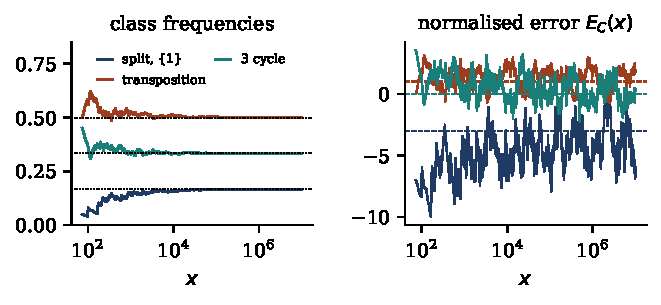
\includegraphics[width=\textwidth]{figs/ch03_chebotarev.pdf}
\caption{Chebotarev for $x^3-x-1$, with Galois group $G=S_3$, primes below $10^7$. Left: frequencies of the three Frobenius classes (split completely, transposition, $3$ cycle) among the unramified primes up to $x$, against $1/6,1/2,1/3$. Right: the normalised error $E_C(x)=(\log x/\sqrt x)\,(|G|\pi_C(x)/|C|-\pi^{\mathrm{ur}}(x))$, where $\pi_C(x)$ and $\pi^{\mathrm{ur}}(x)$ count the unramified primes $p\le x$ with $\Frob_p=C$ and in total; dashed lines mark the limiting means $1-r_C/|C|=-3,1,0$ produced by the prime squares, where $r_C=\#\{g\in G:g^2\in C\}$.}\label{fig:ch03_chebotarev}
\end{figure}

The right panel shows a second order effect. Write $\pi_C(x)$ for the number of unramified $p\le x$ with $\Frob_p=C$, $\pi^{\mathrm{ur}}(x)=\sum_C\pi_C(x)$ for the number of unramified $p\le x$, and $E_C(x)=(\log x/\sqrt x)(|G|\pi_C(x)/|C|-\pi^{\mathrm{ur}}(x))$ for the normalised error. The prime squares enter the explicit formula through $\Frob_p^2$, distributed as $g^2$ for $g$ uniform in $G$. Under the Riemann hypothesis for the Artin $L$ functions of $L$, and since neither $L(s,\rho)$ nor the $L$ function of the sign character, which is the Dirichlet $L$ function of $(-23/\cdot)$, vanishes at $s=\frac12$, $E_C(x)$ is the constant $1-r_C/|C|$, up to $o(1)$, plus an oscillation driven by the zeros whose logarithmic mean is zero (Exercise~\ref{ex:ch3fs}). For $S_3$ the limiting means are $-3$, $1$ and $0$; our logarithmic averages over $10^3<x<10^7$ are $-4.3$, $1.2$ and $0.3$.

The gap is a lower order effect: the limits are approached only at the rate $1/\log x$. The explicit formula counts the prime powers $p^k$ with weight $1/k$, and $\pi_C(x)$ is what remains when the terms with $k\ge2$ are removed. Replacing the number of unramified primes $p\le y$ with $\Frob_p^k=C$ in those terms by its expected value $r_C^{(k)}\operatorname{li}(y)/|G|$ and the number of all unramified primes $p\le y$ by $\operatorname{li}(y)$, with $r_C^{(k)}=\#\{g\in G:g^k\in C\}$ (so $r_C=r_C^{(2)}$) and $\operatorname{li}(y)=\operatorname{Li}(y)+1.045\ldots$ the principal value logarithmic integral, adds $(\log x/\sqrt x)\sum_{k\ge2}k^{-1}(1-r_C^{(k)}/|C|)\operatorname{li}(x^{1/k})$ to $E_C(x)$, and the term $k=2$ equals $(1-r_C/|C|)(1+2/\log x+O(\log^{-2}x))$. The logarithmic means of this sum over $10^3<x<10^7$ are $-4.4$, $1.3$ and $0.2$ if only $k=2,3$ are kept, which is close to the observed values, but the truncation is arbitrary: keeping all $k$ with $2^k\le x$ gives $-5.0$, $1.5$ and $0.3$. The prime powers therefore explain the sign and the order of magnitude of the gap, not its exact value. The smallest primes are not spread over the classes as expected counts assume (the first prime that splits completely is $59$), and the remaining terms of the explicit formula oscillate with amplitude of order one and need not average out over a window of this length. Rubinstein and Sarnak \cite{rubinsteinsarnak1994} put Chebyshev's bias\index{Chebyshev bias} for primes in arithmetic progressions on a probabilistic footing, and their argument extends to Chebotarev classes: under the generalized Riemann hypothesis the law of $E_C(e^y)$, for $y$ uniform in $[0,Y]$, converges as $Y\to\infty$, and under a linear independence hypothesis on the zeros the limit is the law of the constant plus a weighted sum of independent uniformly distributed phases. In our data, primes that split completely are rarer than Chebotarev predicts, $6\pi_{\{1\}}(x)<\pi^{\mathrm{ur}}(x)$, for every $x$ with $2\le x<10^7$ outside $[2.02\times10^6,2.51\times10^6]$, and inside that interval except on short stretches of total length below $10^4$.

\section{Artin \texorpdfstring{$L$}{L} functions and \texorpdfstring{$\ell$}{l} adic representations}\label{sec:ch3artin}

Let $\rho:G_\Q\to\GL(V)$ be a continuous representation on a finite dimensional complex vector space, necessarily with finite image. Artin \cite{artin1924} defined
\[
L(s,\rho)=\prod_p\det\bigl(1-\rho(\Frob_p)p^{-s}\mid V^{I_p}\bigr)^{-1},
\]
where $I_p$ is an inertia group at $p$, $V^{I_p}$ is the subspace it fixes, and $\Frob_p$ acts on $V^{I_p}$ through any of its lifts; the product converges for $\Re s>1$. Brauer's induction theorem \cite{brauer1947} writes $L(s,\rho)$ as a product of integral powers of $L$ functions of one dimensional characters over intermediate fields, which class field theory identifies with Hecke $L$ functions. Hence $L(s,\rho)$ is meromorphic on $\C$ with a functional equation, and holomorphic and nonzero on $\Re s=1$ except for a pole at $s=1$ whose order is the multiplicity of the trivial representation in $\rho$. That is all that Chebotarev requires.\index{Artin $L$ function}

\begin{conjecture}[Artin]
If $\rho$ is irreducible and nontrivial, then $L(s,\rho)$ is entire.
\end{conjecture}

The Artin conjecture follows from reciprocity: if $\rho$ corresponds to a cuspidal automorphic representation of $\GL_n$, then $L(s,\rho)$ is entire by Godement and Jacquet \cite{godementjacquet1972}. For two dimensional $\rho$, odd or even, such a correspondence is known when the projective image is dihedral (Hecke), tetrahedral (Langlands \cite{langlands1980}) or octahedral (Langlands and Tunnell \cite{tunnell1981}). Every odd irreducible two dimensional $\rho$ comes from a weight one newform, by the proof of Serre's modularity conjecture by Khare and Wintenberger \cite{kharewintenberger2009,kharewintenberger2009b}, which also uses work of Kisin \cite{kisin2009}. The even icosahedral case is open, and in dimension three and higher the conjecture is open in general.

Geometry supplies representations with infinite image. For an elliptic curve $E/\Q$ and a prime $\ell$, the $\ell$ adic Tate module\index{Tate module} $T_\ell E=\varprojlim E[\ell^n]$, with $E[\ell^n]$ the $\ell^n$ torsion of $E(\overline{\Q})$, is free of rank $2$ over $\Z_\ell$ with a continuous action of $G_\Q$, giving $\rho_{E,\ell}:G_\Q\to\GL_2(\Z_\ell)$. It is unramified at every $p\nmid\ell N_E$, where $N_E$ is the conductor, and there
\[
\det\bigl(1-\rho_{E,\ell}(\Frob_p)T\bigr)=1-a_pT+pT^2,\qquad a_p=p+1-\#E(\mathbb{F}_p),
\]
independently of $\ell$; by Hasse the reciprocal roots have absolute value $\sqrt p$.

\begin{theorem}[Serre's open image theorem \cite{serre1972}]\label{thm:ch3serre}
Let $E/\Q$ be an elliptic curve without complex multiplication. Then $\rho_{E,\ell}(G_\Q)$ is open in $\GL_2(\Z_\ell)$ for every $\ell$, and equals $\GL_2(\Z_\ell)$ for all but finitely many $\ell$. The image of the adelic representation $G_\Q\to\GL_2(\widehat{\Z})$ is open.
\end{theorem}

Chebotarev, applied to the field cut out by $E[\ell^n]$, shows that the classes of $\rho_{E,\ell}(\Frob_p)\bmod\ell^n$ are equidistributed for the uniform measure on the image of $G_\Q$ in $\GL_2(\Z/\ell^n\Z)$. Hence, when $E$ has no complex multiplication, for all but finitely many $\ell$ and every $d\in\mathbb{F}_\ell^\times$, the residues $a_p\bmod\ell$ over primes $p\equiv d\bmod\ell$ are distributed as the trace of a uniform element of $\GL_2(\mathbb{F}_\ell)$ with determinant $d$. These congruence laws are the correction factors in the Lang and Trotter heuristic of Chapter~\ref{ch:05}. They say nothing about the archimedean size of $a_p/\sqrt p$; that is the content of Sato Tate, and its only known proof goes through automorphy.

The family $(\rho_{E,\ell})_\ell$ is the model of a compatible system\index{compatible system}: representations $\rho_\ell:G_\Q\to\GL_n(\overline{\Q}_\ell)$, one for each prime $\ell$, unramified outside $S\cup\{\ell\}$ for a fixed finite set $S$, such that for each $p\notin S$ the characteristic polynomial of $\rho_\ell(\Frob_p)$, $\ell\ne p$, has coefficients in a fixed number field embedded in every $\overline{\Q}_\ell$ and does not depend on $\ell$. The cohomology $H^i_{\mathrm{et}}(X_{\overline{\Q}},\Q_\ell)$ of a smooth projective variety $X/\Q$ gives one, with $S$ the primes of bad reduction, and by Deligne \cite{deligne1974} for $p\notin S$ the eigenvalues of the geometric Frobenius $\rho_\ell(\Frob_p)^{-1}$ have absolute value $p^{i/2}$.

\section{Reciprocity}\label{sec:ch3recip}

The reciprocity conjecture of Langlands \cite{langlands1970} predicts that every irreducible compatible system arising from geometry corresponds to a cuspidal automorphic representation $\pi$ of $\GL_n(\A_\Q)$: for almost all $p$ the characteristic polynomial of $\rho_\ell(\Frob_p)$ is the Satake polynomial of $\pi_p$, suitably normalised. We record what is known for $n\le2$ over $\Q$ in the cases this book uses.\index{reciprocity}

\subsection{The case \texorpdfstring{$\GL_1$}{GL1}: class field theory}

A continuous character $G_\Q\to\C^\times$ has finite image, so by the Kronecker and Weber theorem it factors through $\Gal(\Q(\zeta_m)/\Q)\cong(\Z/m\Z)^\times$ for some $m$, and is a Dirichlet character. Over a number field $F$, global class field theory identifies the abelianisation of $G_F$ with the group of connected components of the idele class group $F^\times\backslash\A_F^\times$, so that characters of finite order of $G_F$ correspond to Hecke characters of finite order. Reciprocity for $\GL_1$ is a theorem.

\subsection{The case \texorpdfstring{$\GL_2$}{GL2} over \texorpdfstring{$\Q$}{Q}: modularity}

Let $f=\sum a_nq^n$ be a normalised cuspidal newform of weight $k\ge1$, level $N$ and nebentypus $\varepsilon$.

\begin{theorem}[Eichler, Shimura, Deligne, Deligne and Serre]\label{thm:ch3ES}
There is a number field $K_f$ containing the $a_n$, and for each prime $\lambda$ of $K_f$, of residue characteristic $\ell$, a continuous irreducible representation $\rho_{f,\lambda}:G_\Q\to\GL_2(K_{f,\lambda})$ unramified outside $N\ell$ with
\[
\tr\rho_{f,\lambda}(\Frob_p)=a_p,\qquad \det\rho_{f,\lambda}(\Frob_p)=\varepsilon(p)p^{k-1}\qquad(p\nmid N\ell).
\]
For $k=2$ this is due to Eichler \cite{eichler1954} and Shimura \cite{shimura1971}; for $k>2$ to Deligne \cite{deligne1971}, whose proof of the Weil conjectures \cite{deligne1974} then gives $|a_p|\le2p^{(k-1)/2}$; for $k=1$ to Deligne and Serre \cite{deligneserre1974}, who obtain an odd irreducible representation with finite image in $\GL_2(\C)$, unramified outside $N$. Irreducibility for $k\ge2$ is due to Ribet \cite{ribet1977}.
\end{theorem}

Conversely, by the modularity theorem (Theorem~\ref{thm:02modularity}) every elliptic curve $E/\Q$ arises from a newform $f$ of weight $2$ and level $N_E$, so that $L(s,E)=L(s,f)$.\index{modularity theorem} The proof is by modularity lifting, deformation theory matched against Hecke algebras; no probabilistic argument enters.

For the probabilist the Galois side gives congruences, with $\rho(\Frob_p)$ equidistributed in every finite quotient of the image; the automorphic side gives analysis, namely continuation and functional equations for symmetric powers and tensor products. Equidistribution of $a_p/p^{(k-1)/2}$ in $[-2,2]$ is proved through the second, which is why probability enters as a consequence of reciprocity and functoriality (Chapter~\ref{ch:01}).

\section{The dual group and the Satake isomorphism}\label{sec:ch3dual}

Let $G$ be a split connected reductive group over $\Q_p$, with split maximal torus $T$ and root datum $(X^*,\Phi,X_*,\Phi^\vee)$, where $X^*=X^*(T)$ and $X_*=X_*(T)$. The Langlands dual group\index{dual group} $\widehat G$ is the complex reductive group with the dual root datum $(X_*,\Phi^\vee,X^*,\Phi)$. Thus $\GL_n$ is self dual, $\SL_2$ and $\PGL_2$ are dual to each other, and $\mathrm{SO}_{2n+1}$ is dual to $\mathrm{Sp}_{2n}$. For a connected reductive group $G$ over a number field $F$, not necessarily split, the $L$ group is ${}^LG=\widehat G\rtimes W_F$, the Weil group $W_F$ acting through a finite quotient. Regard the split group $G$ as defined over $\Z_p$, let $K=G(\Z_p)$, and let $\mathcal{H}(G(\Q_p),K)$ be the spherical Hecke algebra of compactly supported $K$ biinvariant functions on $G(\Q_p)$ under convolution.

\begin{theorem}[Satake isomorphism \cite{satake1963}]\label{thm:ch3satake}
There is a canonical isomorphism of $\C$ algebras
\[
\mathcal{H}(G(\Q_p),K)\ \cong\ \C[X_*(T)]^{W}\ \cong\ \C[\widehat G]^{\widehat G},
\]
where $W$ is the Weyl group and the last algebra is the algebra of regular class functions on $\widehat G$, spanned by the characters of finite dimensional representations of $\widehat G$.
\end{theorem}

An irreducible smooth representation $\pi_p$ of $G(\Q_p)$ is unramified if it has a nonzero $K$ fixed vector. The space $\pi_p^K$ is then one dimensional, and $\mathcal{H}(G(\Q_p),K)$ acts on it by a character, which by Satake is evaluation at a semisimple conjugacy class $A(\pi_p)\subset\widehat G$, the Satake parameter\index{Satake parameter} of $\pi_p$. The map $\pi_p\mapsto A(\pi_p)$ is a bijection from isomorphism classes of unramified irreducible representations onto semisimple conjugacy classes in $\widehat G$; this is the unramified local Langlands correspondence. For $\GL_2$ and a newform $f$ of weight $k$ with $p\nmid N$, the unitarily normalised Satake parameter is the class of $\operatorname{diag}(\alpha_p,\beta_p)$ with $\alpha_p+\beta_p=a_p/p^{(k-1)/2}$ and $\alpha_p\beta_p=\varepsilon(p)$.

If $\pi_p$ is tempered, as Conjecture~\ref{conj:02ramanujan} predicts for the components of cuspidal representations of $\GL_n$ and as is known for holomorphic newforms, then $A(\pi_p)$ meets a maximal compact subgroup of $\widehat G$. The Hecke operator corresponding to the character $\chi_V$ of a representation $V$ of $\widehat G$ acts on $\pi_p^K$ by $\tr V(A(\pi_p))$. For $\GL_2$, a newform with trivial nebentypus and $V=\Sym^n$ this is $U_n(x_p/2)$ with $x_p=a_p/p^{(k-1)/2}$, the Chebyshev polynomial of the Weyl criterion for $\SU(2)$ in Chapter~\ref{ch:04}; with nontrivial nebentypus the identity fails (Exercise~\ref{ex:ch3neben}). After Satake, the spherical Hecke algebra is the complexified representation ring of the dual group. For $\PGL_2$, Chapter~\ref{ch:07} realises $T_p$ as the adjacency operator of the Bruhat Tits tree, $p+1$ times the transition operator of simple random walk.

\section{The principle of functoriality}\label{sec:ch3funct}

\begin{conjecture}[Functoriality; Langlands \cite{langlands1970}]\label{conj:ch3funct}
Let $G$ and $H$ be connected reductive groups over a number field $F$, with $G$ quasisplit, and let $r:{}^LH\to{}^LG$ be an $L$ homomorphism, that is, a continuous homomorphism compatible with the projections to $W_F$ and holomorphic on $\widehat H$. For every automorphic representation $\pi$ of $H(\A_F)$ there is an automorphic representation $\Pi$ of $G(\A_F)$ such that for almost all places $v$ the Satake parameter of $\Pi_v$ is $r(A(\pi_v))$.
\end{conjecture}

Here, at a finite place $v$ where $H$ and $\pi_v$ are unramified, $A(\pi_v)$ is the Satake parameter of $\pi_v$: a semisimple $\widehat H$ conjugacy class in the coset of ${}^LH$ above a Frobenius element of $W_{F_v}$ \cite{borel1979}, which is the class in $\widehat H$ of Section~\ref{sec:ch3dual} when $H$ is split; the same convention applies to $G$ and $\Pi_v$. The quasisplit hypothesis falls on the target: Jacquet and Langlands transfer from the multiplicative group of a quaternion algebra to $\GL_2$, but not every representation of $\GL_2$ transfers back. Taking $G=\GL_m$ and $r$ an $m$ dimensional representation of ${}^LH$, functoriality predicts that the automorphic $L$ function $L(s,\pi,r)$ is, up to finitely many Euler factors, a standard $L$ function of $\GL_m$, with continuation and a functional equation; see Arthur \cite{arthur2003} and Gelbart \cite{gelbart1984}. Here are the cases we use.\index{functoriality}

\begin{enumerate}
\item Symmetric powers. For $\pi$ on $\GL_2$ and $r=\Sym^n$, functoriality was proved for $n=2$ by Gelbart and Jacquet \cite{gelbartjacquet1978}, for $n=3$ by Kim and Shahidi \cite{kimshahidi2002}, and for $n=4$ by Kim \cite{kimsarnak2003}. Newton and Thorne \cite{newtonthorne2021,newtonthorne2021b} proved it for every $n$ when $\pi$ comes from a holomorphic newform of weight $k\ge2$ without complex multiplication. For Maass forms the cases $n\ge5$ are open.
\item Base change for $\GL_n$ along cyclic extensions of prime degree, and so along solvable Galois extensions by iteration, by Langlands \cite{langlands1980} for $n=2$ and Arthur and Clozel \cite{arthurclozel1989} for general $n$.
\item Jacquet Langlands. If $D$ is a quaternion algebra over $F$, Jacquet and Langlands \cite{jacquetlanglands1970} transferred automorphic representations of $D^\times(\A_F)$ of dimension greater than one to cuspidal representations of $\GL_2(\A_F)$, discrete series where $D$ ramifies. This identifies Hecke eigenvalues on the supersingular isogeny graphs of Chapter~\ref{ch:08} with Fourier coefficients of modular forms.
\item Tensor products. $\GL_2\times\GL_2\to\GL_4$ is functorial by Ramakrishnan \cite{ramakrishnan2000}, and $\GL_2\times\GL_3\to\GL_6$ by Kim and Shahidi \cite{kimshahidi2002}. The general case is open.
\end{enumerate}

The local Langlands correspondence\index{local Langlands correspondence} for $\GL_n$ over a finite extension $F_v$ of $\Q_p$ is a bijection from isomorphism classes of irreducible smooth representations of $\GL_n(F_v)$ to isomorphism classes of $n$ dimensional Frobenius semisimple Weil Deligne representations of $W_{F_v}$, characterised by local class field theory for $n=1$ and by compatibility with twists, central characters, duals and the $L$ and $\varepsilon$ factors of pairs. On unramified representations it is the bijection $\pi_p\mapsto A(\pi_p)$ of Section~\ref{sec:ch3dual}. It was proved by Harris and Taylor \cite{harristaylor2001} and by Henniart \cite{henniart2000}, with a later proof by Scholze \cite{scholze2013}.

\subsection{Potential automorphy and the Sato Tate theorem}

The Sato Tate theorem was proved before Newton and Thorne, from a weaker statement. A compatible system over a number field $F$ is potentially automorphic if its restriction to $G_{F'}$ is automorphic for some finite Galois extension $F'/F$; in the results quoted next, $F'$ can be chosen totally real when $F$ is. Clozel, Harris and Taylor \cite{cht2008}, Taylor \cite{taylor2008}, and Harris, Shepherd Barron and Taylor \cite{hsbt2010} proved potential automorphy of the odd symmetric powers $\Sym^{2m-1}\rho_{E,\ell}$ for elliptic curves over totally real fields with nonintegral $j$ invariant, which together with Rankin Selberg theory controls every symmetric power $L$ function. Barnet Lamb, Geraghty, Harris and Taylor \cite{blght2011} proved potential automorphy of all symmetric powers of holomorphic newforms of weight $k\ge2$ without complex multiplication, and noted that the hypothesis on the $j$ invariant can now be removed for elliptic curves without complex multiplication over totally real fields.

Potential automorphy suffices because Brauer's induction theorem, applied to $\Gal(F'/F)$, expresses $L(s,\Sym^n\rho)$ as a product of integral powers of $L$ functions over intermediate fields. The subgroups in Brauer's theorem are elementary, hence solvable, so solvable descent \cite{arthurclozel1989} makes these standard or Rankin Selberg $L$ functions of automorphic representations. Each is nonvanishing on $\Re s\ge1$ by the results of Jacquet and Shalika \cite{jacquetshalika1976} and Shahidi \cite{shahidi1981}, and holomorphic there except for the simple pole at $s=1$ of the Rankin Selberg factors $L(s,\pi\times\tilde\pi)$, which cancels in $L(s,\Sym^n\rho)$ for $n\ge1$. So $L(s,\Sym^n\rho)$ is meromorphic on $\C$, and holomorphic and nonzero on $\Re s\ge1$ for $n\ge1$, though not known from this argument to be entire. This is exactly the hypothesis of Serre's theorem (Theorem~\ref{thm:04serre}).

\begin{theorem}[Sato Tate; Clozel, Harris, Shepherd Barron, Taylor, Barnet Lamb, Geraghty]\label{thm:ch3ST}
Let $E/\Q$ be an elliptic curve without complex multiplication and, for $p\nmid N_E$, write $a_p=2\sqrt p\cos\theta_p$ with $\theta_p\in[0,\pi]$. Then $(\theta_p)$ is equidistributed with respect to $\frac2\pi\sin^2\theta\,d\theta$.
\end{theorem}

The proof is the archetype of the slogan that functoriality implies probability: potential automorphy gives the analysis of $L(s,\Sym^n E)$ for every irreducible representation $\Sym^n$ of $\SU(2)$, and the Weyl criterion converts it into a law of large numbers; Chapter~\ref{ch:04} gives the details. Harris~\cite{harris2009} proved the joint version, assuming results on Galois representations that were established soon afterwards: for two elliptic curves over a totally real field, without complex multiplication and not isogenous over an algebraic closure, the pairs $(\theta_p,\theta'_p)$ are equidistributed for the product of the two Sato Tate measures (over $\Q$ this is Theorem~\ref{thm:04joint}, where the hypotheses are discussed).

\section{The Sato Tate group}\label{sec:ch3stgroup}

Which compact group replaces $\SU(2)$ for a general motive? Serre gave the definition \cite{serre2012}, and Fité, Kedlaya, Rotger and Sutherland \cite{fkrs2012} showed that for abelian surfaces it is determined by the Galois module of endomorphisms. Let $A$ be an abelian variety of dimension $g$ over a number field $F$.\index{Sato Tate group}

\begin{definition}[Serre]\label{def:ch3stgroup}
Fix a prime $\ell$ and let $\rho_\ell:G_F\to\mathrm{GSp}_{2g}(\Q_\ell)$ be the action on $V_\ell A=T_\ell A\otimes\Q_\ell$, symplectic for the Weil pairing of a polarisation. Let $G_\ell$ be the Zariski closure of $\rho_\ell(G_F)$ in $\mathrm{GSp}_{2g}$, and $G^1_\ell=G_\ell\cap\mathrm{Sp}_{2g}$. Choose a field embedding $\iota:\Q_\ell\to\C$. The Sato Tate group $\mathrm{ST}(A)$ is a maximal compact subgroup of $G^1_\ell\otimes_\iota\C$, a compact subgroup of $\USp(2g)$ well defined up to conjugacy.
\end{definition}

For a prime $\mathfrak{p}\nmid\ell$ of $F$ at which $A$ has good reduction, with norm $N\mathfrak{p}$, the normalised Frobenius $\iota\rho_\ell(\Frob_{\mathfrak{p}})/\sqrt{N\mathfrak{p}}$ lies in $G^1_\ell(\C)$ and is semisimple with eigenvalues of absolute value one, so it defines a conjugacy class $s_{\mathfrak{p}}$ in $\mathrm{ST}(A)$. Independence of $\ell$ and $\iota$ is known for $g\le3$. Let $K$ be the smallest extension of $F$ over which all endomorphisms of $A$ are defined. Then $\Gal(K/F)$ is a quotient of the component group $\mathrm{ST}(A)/\mathrm{ST}(A)^0$, and the two are isomorphic when $g\le3$ \cite{banaszakkedlaya2015,fkrs2012,sutherland2019}, so that Chebotarev for $K/F$ governs which component contains $s_{\mathfrak{p}}$; for general $g$ the same role is played by the extension of $F$ cut out by the component group, which contains $K$.

\begin{conjecture}[Generalised Sato Tate]\label{conj:ch3gst}
The classes $s_{\mathfrak{p}}$, over the primes $\mathfrak{p}$ of good reduction ordered by norm, are equidistributed with respect to the pushforward of Haar measure on $\mathrm{ST}(A)$ to its space of conjugacy classes.
\end{conjecture}

For an elliptic curve $E/F$ without complex multiplication over $\overline F$ the group is $\mathrm{ST}(E)=\SU(2)=\USp(2)$. For $E$ with complex multiplication by an imaginary quadratic field $M$, the group is $\mathrm{U}(1)$ if $M\subseteq F$ and its normaliser $N(\mathrm{U}(1))$ in $\SU(2)$ otherwise; the pushforward of Haar measure on $N(\mathrm{U}(1))$ to the trace is the law $\mu_{\mathrm{CM}}=\tfrac12\delta_0+\tfrac12$ arcsine of Section~\ref{sec:04cm}, with Weyl averages in Proposition~\ref{prop:04cm}.

\begin{theorem}[Fité, Kedlaya, Rotger and Sutherland \cite{fkrs2012}]\label{thm:ch3fkrs}
Up to conjugacy in $\USp(4)$, there are exactly $52$ compact groups that occur as Sato Tate groups of abelian surfaces over number fields, and $34$ of them occur over $\Q$. Their identity components are $\mathrm{U}(1)$, $\SU(2)$, $\mathrm{U}(1)\times\mathrm{U}(1)$, $\mathrm{U}(1)\times\SU(2)$, $\SU(2)\times\SU(2)$ and $\USp(4)$.
\end{theorem}

For abelian surfaces Conjecture~\ref{conj:ch3gst} is open in the generic case $\mathrm{ST}(A)=\USp(4)$, which occurs exactly when $\operatorname{End}(A_{\overline F})=\Z$, as for the Jacobian of a typical genus $2$ curve; Johansson \cite{johansson2017} proved many of the nongeneric cases from the potential automorphy theorems. Kedlaya and Sutherland \cite{kedlayasutherland2009} compare moments of normalised $L$ polynomial coefficients over large ranges of primes with those of candidate groups, and for dimension three Fité, Kedlaya and Sutherland \cite{fks2021} announced a classification with $410$ groups. Chebotarev governs the components; automorphy governs the identity component. Chapter~\ref{ch:12} turns the moment comparison into a consistent Bayesian model selection.

\section{Notes}

Frobenius's density theorem (1896) gives the density of the primes whose Frobenius generates a given cyclic subgroup up to conjugacy, hence of each factorisation type, and is a weaker form of Chebotarev's; Chebotarev's device of adjoining roots of unity was then used by Artin to prove his reciprocity law \cite{artin1927}. For the elliptic curve analogue of Chebyshev's bias see Sarnak's letter to Mazur \cite{sarnak2007} and Mazur's survey \cite{mazur2008}. Borel's Corvallis article \cite{borel1979} remains the standard account of $L$ groups. Beyond the cases listed in Section~\ref{sec:ch3funct}, the stabilisation of the trace formula, which rests on Ngô's proof of the fundamental lemma \cite{ngo2010}, underlies Arthur's classification of the automorphic representations of quasisplit symplectic and orthogonal groups, which includes their transfer to general linear groups \cite{arthur2013}. Serre's book \cite{serre2012} treats Sato Tate groups, with Sutherland's survey \cite{sutherland2019} as a computational companion. Rouse, Sutherland and Zureick Brown \cite{rszb2022} classified the $\ell$ adic images of Galois for elliptic curves over $\Q$ without complex multiplication, up to the possible existence of unexpected rational points on the modular curves $X_{\mathrm{ns}}^+(\ell)$ of nonsplit Cartan type for primes $\ell\ge19$ and on six further modular curves, of levels $25$, $27$, $49$ and $121$.

\section{Exercises}

\begin{enumerate}
\item Let $f=x^3-x-1$ and let $N_p$ be the number of roots of $f$ modulo $p$. Show that $N_p$ converges in law, along primes, to the number of fixed points of a uniform permutation in $S_3$. Deduce that the mean of $N_p$ tends to $1$ and its second moment to $2$, and check these against the frequencies $0.16637$, $0.50027$, $0.33336$ observed below $10^7$.
\item (Burnside) Let $f\in\Z[x]$ be monic and irreducible with Galois group $G$, and let $N_p$ be the number of roots of $f$ modulo $p$. Prove that the average of $N_p$ over primes $p\le x$ tends to $1$, and that the limiting $k$th factorial moment of $N_p$ equals the number of orbits of $G$ on ordered $k$ tuples of distinct roots.
\item Let $A$ be Haar distributed in $\SU(2)$ and $t=\tr A$. Show that the characters $\tr\Sym^m(A)$ are orthonormal in $L^2$ of Haar measure and that $\tr\Sym^2(A)=t^2-1$. Deduce from Theorem~\ref{thm:ch3ST} that if $E/\Q$ has no complex multiplication then $\pi(x)^{-1}\sum_{p\le x,\,p\nmid N_E}(a_p^2/p-1)\to0$. Then prove the same limit for every $E/\Q$, with or without complex multiplication, using only the Rankin Selberg $L$ function $L(s,f\times f)$ of the newform $f$ attached to $E$. (Hint: $\log L(s,f\times f)$ has nonnegative Dirichlet coefficients, and $L(s,f\times f)$ continues meromorphically with a simple pole at $s=1$ and no other pole or zero on $\Re s=1$; apply the Wiener Ikehara theorem of Chapter~\ref{ch:04}.)
\item Let $\Gamma$ be one of $\SU(2)$, $N(\mathrm{U}(1))$ or $\USp(4)$, and let $t=\tr\gamma$ for a Haar random $\gamma\in\Gamma$. Show that $(\E t^2,\E t^4,\E t^6)$ equals $(1,2,5)$, $(1,3,10)$ and $(1,3,14)$ respectively, using the Weyl density \eqref{eq:ch6usp} of Chapter~\ref{ch:06} for $\USp(4)$. Conclude that $N(\mathrm{U}(1))$ and $\USp(4)$ are not separated by second and fourth moments, and explain how the proportion of primes with Frobenius trace $0$ separates them.
\item\label{ex:ch3fs} Let $G$ be a finite group, $C$ a conjugacy class, $r_C=\#\{g\in G:g^2\in C\}$, and $\varepsilon_\chi=|G|^{-1}\sum_{g\in G}\chi(g^2)$ the Frobenius Schur indicator of an irreducible character $\chi$. Show that $\sum_\chi\varepsilon_\chi\overline{\chi(C)}=r_C/|C|$, the sum running over all irreducible characters. With $\pi_\chi(x)=\sum_{p\le x,\,p\nmid d_L}\chi(\Frob_p)$, show that $|G|\pi_C(x)/|C|-\pi^{\mathrm{ur}}(x)=\sum_{\chi\ne1}\overline{\chi(C)}\,\pi_\chi(x)$, and deduce that if each $(\log x/\sqrt x)\pi_\chi(x)$, $\chi\ne1$, has logarithmic mean $-\varepsilon_\chi$, then $E_C$ has logarithmic mean $1-r_C/|C|$. Check the values $-3$, $1$, $0$ for $S_3$, and show that $\sum_C|C|(1-r_C/|C|)=0$ for every $G$.
\item\label{ex:ch3neben} Let $A=\operatorname{diag}(\alpha,\beta)$ with $\alpha\beta=1$. Show that $\tr\Sym^nA=U_n(\tr A/2)$ for every $n\ge0$. If instead $\alpha\beta=\varepsilon$ with $|\varepsilon|=1$, show that $\tr\Sym^nA=\eta^nU_n(\tr A/(2\eta))$ for either square root $\eta$ of $\varepsilon$; in particular $\tr\Sym^2A=(\tr A)^2-\varepsilon$, so for a newform with nontrivial nebentypus the Weyl averages of $U_n(x_p/2)$ are the wrong test of equidistribution.
\end{enumerate}

\section{Open computational problems}

\begin{compproblem}[Chebotarev statistics and bias races]
Objective: measure the convergence rate and the bias in Chebotarev's theorem for nonabelian Galois groups at scale. Objects: the splitting fields of $x^3-x-1$ ($S_3$), of $x^4-x-1$ ($S_4$, discriminant $-283$) and of $x^5+20x+16$ ($A_5$, discriminant $2^{16}5^6$); all primes $p\le10^{10}$. Route: factor $f$ modulo $p$ by computing $x^p$ modulo $f$ on GPUs, separating the two classes of $5$ cycles in $A_5$, which share a cycle type, by a resolvent or a $p$ adic Frobenius algorithm in PARI/GP; compute the first $10^4$ zeros of each Artin $L$ function with \texttt{lfun}, using weight one forms in LMFDB where they exist. Deliverable: tables of $\pi_C(x)$ at $x=10^k$, plots of $E_C(e^y)$, the logarithmic densities of $\{E_C>E_{C'}\}$, and a comparison with the Rubinstein and Sarnak model built from the computed zeros. Why it matters: the bias measures Galois structure ($r_C$) and the low zeros of Artin $L$ functions, and the comparison tests consequences of the linear independence hypothesis in a nonabelian setting.
\end{compproblem}

\begin{compproblem}[Empirical Sato Tate groups in genus $2$ and $3$]
Objective: assign a Sato Tate group to every curve in a large database from Frobenius data alone, with calibrated confidence. Objects: all genus $2$ curves in LMFDB (about $66{,}000$) and a comparable sample of genus $3$ curves, with $L$ polynomials at all good primes $p\le2^{30}$. Route: point counting in the style of Kedlaya and Sutherland, or the average polynomial time computation of Hasse Witt matrices of Harvey and Sutherland \cite{harveysutherland2014} for hyperelliptic curves, which gives the $L$ polynomial modulo $p$ and, in genus at most $3$, is completed by a generic group algorithm; moment sequences of the coefficients $a_1,a_2$ of the normalised $L$ polynomial and the proportion of primes with $a_1=0$; the sequential Bayesian test of Chapter~\ref{ch:12} with the $52$ candidate measures of \cite{fkrs2012} and the $410$ of \cite{fks2021}. Deliverable: a table of posterior probabilities, agreement rates with the endomorphism data in LMFDB, and the number of primes needed for a posterior of $1-10^{-6}$ as a function of the group. Why it matters: it turns Conjecture~\ref{conj:ch3gst} into a calibrated statistical procedure and flags curves with atypical Frobenius data.
\end{compproblem}

\begin{compproblem}[Joint Sato Tate independence]
Objective: test the asymptotic independence of Frobenius angles at the same prime for unrelated motives, and measure the rate. Objects: pairs of elliptic curves over $\Q$ of conductor below $10^4$, without complex multiplication and not isogenous over $\overline{\Q}$, with all primes below $10^9$; a random sample of $10^4$ pairs $(E,f)$ with $E$ as before and $f$ a newform of weight $4$, trivial nebentypus and level at most $100$, without complex multiplication, with all primes below $10^7$; and, as a control, pairs $(E,E^{(D)})$ with $E^{(D)}$ a quadratic twist, for which $\theta'_p$ equals $\theta_p$ or $\pi-\theta_p$ according as $(D/p)=1$ or $-1$, so that the pairs $(\theta_p,\theta'_p)$ lie on the two diagonals of $[0,\pi]^2$ with frequency $\tfrac12$ each. Route: PARI/GP \texttt{ellap} in batch for the curves and \texttt{mfcoefs} (after \texttt{mfinit} and \texttt{mfeigenbasis}) for $f$, in a fixed real embedding of its coefficient field, or average polynomial time algorithms for the curves; joint Weyl averages $\pi(x)^{-1}\sum_{p\le x}U_m(x_p/2)U_n(x'_p/2)$ for $0\le m,n\le20$, $(m,n)\ne(0,0)$, a two dimensional discrepancy, and a permutation test that shuffles one sequence across primes. Deliverable: heat maps of the Weyl averages, the growth of $\sqrt{\pi(x)}$ times the discrepancy, and test statistics with null distributions. Why it matters: joint equidistribution holds in the first two cases, by symmetric power functoriality and Rankin Selberg theory (Theorem~\ref{thm:04joint} for two curves over $\Q$), and its rate is governed by the zeros of $L(s,\Sym^mE\times\Sym^nE')$, where $E'$ is the second curve or, for the pairs $(E,f)$, the form $f$, so the data probe the Riemann hypothesis for these $L$ functions.
\end{compproblem}

\part{Equidistribution}
\chapter{Haar Measure, the Weyl Criterion and Sato Tate}\label{ch:04}

In 1916 Hermann Weyl showed that a sequence in $[0,1)$ is equidistributed if and only if the averages of the characters $e^{2\pi i h x}$ along it tend to zero for every integer $h \neq 0$ \cite{weyl1916}. He used the criterion to reprove the equidistribution of the fractional parts of $n\alpha$ for irrational $\alpha$, found around 1910 by Bohl, Sierpi\'nski and Weyl himself, and to extend it to polynomial sequences; the criterion has outlived the problem. The Peter Weyl theorem \cite{peterweyl1927}, proved in 1927 for compact Lie groups, makes the matrix coefficients of irreducible representations dense among continuous functions and so gives the same criterion on compact groups, with irreducible characters in place of exponentials. In the early 1960s Sato and Tate, working independently and from quite different directions, predicted that the angles of Frobenius of an elliptic curve over $\Q$ without complex multiplication are distributed according to the image of Haar measure on $\SU(2)$ \cite{tate1965}. Serre saw that Weyl's criterion converts this prediction into a statement about $L$ functions \cite{serre1968}: the conjecture follows if every symmetric power $L$ function is holomorphic and nonvanishing on the line $\Re s = 1$. That statement is a consequence of functoriality. For elliptic curves over $\Q$ and holomorphic newforms it was proved through potential automorphy in papers published between 2008 and 2011, and in 2021 Newton and Thorne proved that every symmetric power is automorphic; this is one of the clearest successes of the Langlands programme. We prove the probabilistic side completely and state the arithmetic input precisely. The logical direction matters throughout: automorphy is the input, equidistribution is the output.

\section{Equidistribution on compact metric spaces}

Let $X$ be a compact metric space and $\mu$ a Borel probability measure on $X$. A sequence $(x_j)$ in $X$ is \emph{equidistributed} with respect to $\mu$ if the empirical measures $\nu_n = n^{-1}\sum_{j\le n}\delta_{x_j}$ converge weakly to $\mu$, that is $\int f\,d\nu_n \to \int f\,d\mu$ for every $f \in C(X)$.\index{equidistribution} For sequences indexed by primes we use the ordering by size, so the natural normalisation is $\pi(x)^{-1}\sum_{p\le x}$.

Weak convergence can be tested on any family of functions whose linear span is dense in $C(X)$ for the supremum norm. This observation is the whole content of the Weyl criterion; what makes it useful is that representation theory supplies a canonical dense family. For the circle $\R/\Z$ the family is $x \mapsto e^{2\pi ihx}$, $h \in \Z$, whose span is dense by Fej\'er's theorem; this recovers Weyl's original criterion. We shall also use the portmanteau theorem: if $\nu_n \to \mu$ weakly, then $\limsup \nu_n(F) \le \mu(F)$ for every closed $F \subset X$.

\section{Peter Weyl and Schur orthogonality}

Let $K$ be a compact metrisable group, for instance a closed subgroup of $\mathrm{U}(n)$, with normalised Haar measure $h$. Representations of $K$ are continuous and finite dimensional. A \emph{class function} is a function constant on conjugacy classes. Write $K^\natural$ for the space of conjugacy classes with the quotient topology, a compact metrisable space, and $h^\natural$ for the pushforward of $h$. Continuous class functions on $K$ are exactly the continuous functions on $K^\natural$. For a representation $\rho$ of $K$ we write $\chi_\rho = \tr \rho$ for its character.

\begin{theorem}[Schur orthogonality]\index{Schur orthogonality}
If $\rho$ and $\sigma$ are irreducible representations of $K$, then
\[
\int_K \chi_\rho(g)\overline{\chi_\sigma(g)}\,dh(g) =
\begin{cases} 1 & \rho \cong \sigma,\\ 0 & \text{otherwise.}\end{cases}
\]
In particular $\int \chi_\rho\,dh = 0$ for every nontrivial irreducible $\rho$.
\end{theorem}

\begin{theorem}[Peter and Weyl \cite{peterweyl1927}]\index{Peter Weyl theorem}
Matrix coefficients of finite dimensional irreducible representations span a dense subspace of $C(K)$. Consequently the characters of irreducible representations span a dense subspace of the continuous class functions on $K$.
\end{theorem}

The second statement follows from the first. The averaging operator $P\phi(g) = \int_K \phi(kgk^{-1})\,dh(k)$ fixes class functions, does not increase the supremum norm, and, by Schur's lemma, maps each matrix coefficient of an irreducible $\rho$ to a multiple of $\chi_\rho$. So if a class function $f$ satisfies $\|f - \phi\|_\infty < \delta$ for a combination $\phi$ of matrix coefficients, then $\|f - P\phi\|_\infty < \delta$, and $P\phi$ is a combination of irreducible characters.

\section{The Weyl criterion on compact groups}

We prove the form of the criterion used throughout the book.

\begin{theorem}[Weyl criterion \cite{weyl1916,serre1968}]\label{thm:04weyl}\index{Weyl criterion}
Let $K$ be a compact metrisable group and $(\theta_p)$ a sequence in $K^\natural$ indexed by primes. Then $(\theta_p)$ is equidistributed with respect to $h^\natural$ if and only if, for every nontrivial irreducible representation $\rho$ of $K$,
\[
\lim_{x\to\infty}\frac{1}{\pi(x)}\sum_{p\le x}\chi_\rho(\theta_p) = 0 .
\]
More generally, $(\theta_p)$ is equidistributed with respect to a probability measure $\mu$ on $K^\natural$ if and only if $\pi(x)^{-1}\sum_{p\le x}\chi_\rho(\theta_p) \to \int \chi_\rho\,d\mu$ for every irreducible $\rho$.
\end{theorem}

\begin{proof}
We prove the general statement; the first follows from Schur orthogonality, which gives $\int \chi_\rho\,dh^\natural = 0$ for nontrivial $\rho$ and $1$ for the trivial representation. Write $\nu_x = \pi(x)^{-1}\sum_{p\le x}\delta_{\theta_p}$.

Necessity is immediate: each $\chi_\rho$ is continuous on $K^\natural$.

For sufficiency, let $f \in C(K^\natural)$ and $\delta > 0$. By the Peter Weyl theorem there is a finite linear combination $g = \sum_\rho c_\rho\chi_\rho$ with $\|f - g\|_\infty < \delta$. By hypothesis and linearity, $\int g\,d\nu_x \to \int g\,d\mu$. Then
\[
\Bigl|\int f\,d\nu_x - \int f\,d\mu\Bigr|
\le \Bigl|\int (f-g)\,d\nu_x\Bigr| + \Bigl|\int g\,d\nu_x - \int g\,d\mu\Bigr| + \Bigl|\int (g-f)\,d\mu\Bigr| ,
\]
and the first and third terms are each at most $\delta$ because $\nu_x$ and $\mu$ are probability measures. Hence $\limsup_x |\int f\,d\nu_x - \int f\,d\mu| \le 2\delta$ for every $\delta > 0$, and the limit is $0$.
\end{proof}

The proof uses only that each $\nu_x$ is a probability measure on $K^\natural$. The criterion therefore holds for any sequence of probability measures on $K^\natural$, for instance the empirical measures $n^{-1}\sum_{j\le n}\delta_{\theta_j}$ of a sequence indexed by the integers, or those of the finite families of conjugacy classes that arise in vertical problems (Chapter~\ref{ch:06b}).

The limits $\int \chi_\rho\,d\mu$ for a measure other than Haar are themselves informative: when $\mu$ is the image of Haar measure on a closed subgroup $H \subset K$, the integral is the multiplicity of the trivial representation in $\rho|_H$, a nonnegative integer. We call the function $\rho \mapsto \int \chi_\rho\,d\mu$ on the irreducible representations of $K$ the \emph{Weyl fingerprint}\index{Weyl fingerprint} of $\mu$; for $\SU(2)$ it is a sequence indexed by $n \ge 0$ (next section).

\section{The group SU(2)}

Every element of $\SU(2)$ is conjugate to $\operatorname{diag}(e^{i\theta}, e^{-i\theta})$ for a unique $\theta \in [0,\pi]$, so $\SU(2)^\natural$ is identified with $[0,\pi]$, and equally with the interval $[-2,2]$ through the trace $x = 2\cos\theta$. The irreducible representations are the symmetric powers $\Sym^n$ of the standard representation, of dimension $n+1$, with eigenvalues $e^{i(n-2j)\theta}$ for $0\le j\le n$. Summing the geometric progression,
\[
\chi_n(\theta) = \tr\Sym^n(\theta) = \sum_{j=0}^n e^{i(n-2j)\theta} = \frac{\sin((n+1)\theta)}{\sin\theta} = U_n(\cos\theta) = U_n(x/2),
\]
where $U_n$ is the Chebyshev polynomial of the second kind.\index{Chebyshev polynomials} The recurrence $U_1(t)U_n(t) = U_{n+1}(t) + U_{n-1}(t)$ is the Clebsch Gordan rule $\mathrm{std}\otimes\Sym^n \cong \Sym^{n+1}\oplus\Sym^{n-1}$.

\begin{proposition}[Weyl integration formula for $\SU(2)$]\index{Weyl integration formula}
The pushforward of Haar measure to $[0,\pi]$ is $\frac{2}{\pi}\sin^2\theta\,d\theta$. Equivalently, the trace $x = 2\cos\theta$ of a Haar random element has the semicircle law
\[
\ST(dx) = \frac{1}{2\pi}\sqrt{4 - x^2}\,dx, \qquad x \in [-2,2].
\]
\end{proposition}

\begin{proof}
Identify $\SU(2)$ with the unit quaternions $S^3$; Haar measure is normalised surface measure, since multiplications by unit quaternions are isometries. The trace is $2a$ for $g = a + bi + cj + dk$, and the slice $\{a = \cos\theta\}$ is a two sphere of radius $\sin\theta$, so surface measure on $S^3$ projects to a density proportional to $\sin^2\theta$ on $[0,\pi]$. Since $\int_0^\pi \sin^2\theta\,d\theta = \pi/2$, the normalised density is $\frac{2}{\pi}\sin^2\theta$. Changing variables $x = 2\cos\theta$, $dx = -2\sin\theta\,d\theta$ and $\sin\theta = \frac12\sqrt{4-x^2}$ gives the semicircle.
\end{proof}

\begin{proposition}[Orthonormality and Catalan moments]\label{prop:04catalan}
The polynomials $U_n(x/2)$ are orthonormal in $L^2(\ST)$, and
\[
\int_{-2}^2 x^{k}\,\ST(dx) = \begin{cases} C_m = \dfrac{1}{m+1}\dbinom{2m}{m} & k = 2m,\\[4pt] 0 & k \text{ odd.}\end{cases}
\]
\end{proposition}

\begin{proof}
In the variable $\theta$, the factors $\sin\theta$ cancel against the density $\frac{2}{\pi}\sin^2\theta$, and
\[
\int U_m(x/2)\,U_n(x/2)\,\ST(dx) = \frac{2}{\pi}\int_0^\pi \sin((m+1)\theta)\sin((n+1)\theta)\,d\theta = \delta_{mn}
\]
by orthogonality of sines on $[0,\pi]$.

For the moments, iterate the Clebsch Gordan rule. Since $x = U_1(x/2)$, we have $x\,U_n(x/2) = U_{n+1}(x/2) + U_{n-1}(x/2)$ for $n \ge 1$ and $x\,U_0(x/2) = U_1(x/2)$. By induction $x^k = \sum_{n\ge0} N_k(n)\,U_n(x/2)$, where $N_k(n)$ is the number of paths of $k$ steps $\pm1$ on the nonnegative integers from $0$ to $n$ that never go below $0$. By orthonormality, $\int x^k\,d\ST = N_k(0)$, the number of Dyck paths of length $k$. This vanishes for $k$ odd, and for $k = 2m$ the reflection principle gives $N_{2m}(0) = \binom{2m}{m} - \binom{2m}{m+1} = C_m$.
\end{proof}

The moments of $\ST$ thus count returning paths of the simple walk on the nonnegative integers. Spectral measures whose moments count returning paths recur throughout the book; in Chapter~\ref{ch:07} the same computation on a regular tree produces the Kesten McKay laws.

\section{The Sato Tate conjecture and Serre's theorem}

Let $E/\Q$ be an elliptic curve of conductor $N$. For $p \nmid N$ put $a_p = p + 1 - \#E(\mathbb{F}_p)$. Hasse's bound $|a_p| \le 2\sqrt p$ says that $x_p = a_p/\sqrt p$ lies in $[-2,2]$, so we may write $x_p = 2\cos\theta_p$ with $\theta_p \in [0,\pi]$, and regard $\theta_p$ as the conjugacy class in $\SU(2)$ of the normalised Frobenius. More generally, for a holomorphic newform $f = \sum a_n q^n$ of weight $k \ge 2$, level $N$ and trivial character, Deligne's theorem \cite{deligne1974} gives $|a_p| \le 2p^{(k-1)/2}$ for $p \nmid N$, and we set $x_p = a_p/p^{(k-1)/2}$.

\begin{conjecture}[Sato and Tate]\index{Sato Tate conjecture}
If $E/\Q$ has no complex multiplication, the angles $\theta_p$ are equidistributed in $[0,\pi]$ with respect to $\frac{2}{\pi}\sin^2\theta\,d\theta$; equivalently $(x_p)$ is equidistributed with respect to $\ST$.
\end{conjecture}

The conjecture is now a theorem, and we explain how. The analytic objects are the symmetric power $L$ functions. Write the normalised Satake parameters at a good prime as $\{\alpha_p, \beta_p\} = \{e^{i\theta_p}, e^{-i\theta_p}\}$ and define, for $n \ge 1$,
\[
L(s, \Sym^n f) = \prod_{p\nmid N}\prod_{j=0}^n \bigl(1 - \alpha_p^{j}\beta_p^{n-j}p^{-s}\bigr)^{-1},
\]
which converges absolutely for $\Re s > 1$. (Including suitable factors at the finitely many bad primes changes nothing below, because those factors are holomorphic and nonvanishing on $\Re s > 0$.) The tool that converts analytic information on $\Re s = 1$ into asymptotics is the Tauberian theorem of Wiener and Ikehara \cite{wiener1932,wienerikehara1931}.

\begin{theorem}[Wiener and Ikehara]\index{Wiener Ikehara theorem}
Let $F(s) = \sum_{n\ge1} b_n n^{-s}$ with $b_n \ge 0$, convergent for $\Re s > 1$. Suppose there is a constant $c$ such that $F(s) - c/(s-1)$ extends to a continuous function on the closed half plane $\Re s \ge 1$. Then $\sum_{n\le x} b_n \sim c\,x$ as $x \to \infty$.
\end{theorem}

The prime number theorem is the case $F = -\zeta'/\zeta$, $b_n = \Lambda(n)$, $c = 1$, the hypothesis being that $\zeta$ has no zeros on $\Re s = 1$.

\begin{theorem}[Serre \cite{serre1968}]\label{thm:04serre}
Let $f$ be a holomorphic newform of weight $k\ge2$ with trivial character. Suppose that for every $n \ge 1$ the function $L(s, \Sym^n f)$ extends holomorphically to an open set containing $\Re s \ge 1$ and has no zeros on $\Re s = 1$. Then $(x_p)$ is equidistributed with respect to $\ST$.
\end{theorem}

\begin{proof}
Sums over primes in this proof run over $p \nmid N$; omitting finitely many primes changes no limit below. Fix $n \ge 1$. Taking the logarithmic derivative of the Euler product,
\[
-\frac{L'}{L}(s,\Sym^n f) = \sum_{p\nmid N}\sum_{m\ge1}\Bigl(\sum_{j=0}^n (\alpha_p^j\beta_p^{n-j})^m\Bigr)\log p\,p^{-ms}.
\]
The term $m = 1$ has coefficient $\tr\Sym^n(\theta_p)\log p = U_n(x_p/2)\log p$. Each inner sum has absolute value at most $n+1$ because $|\alpha_p| = |\beta_p| = 1$, so the terms with $m \ge 2$ form a series dominated by $(n+1)\sum_p \log p \sum_{m\ge2}p^{-m\sigma}$, which converges uniformly on $\Re s \ge \sigma_0$ for any $\sigma_0 > 1/2$. Hence
\[
D_n(s) := \sum_{p} U_n(x_p/2)\log p\,p^{-s} = -\frac{L'}{L}(s,\Sym^n f) - H_n(s),
\]
with $H_n$ holomorphic on $\Re s > 1/2$. By hypothesis $L(s,\Sym^n f)$ is holomorphic and zero free on a neighbourhood of $\Re s \ge 1$ (on $\Re s > 1$ the Euler product does not vanish), so $D_n$ extends holomorphically to a neighbourhood of $\Re s \ge 1$.

The coefficients of $D_n$ are not of one sign, so we add a multiple of the prime number theorem. Let $\vartheta(s) = \sum_p \log p\,p^{-s}$; by the same estimate, and because the finitely many terms with $p \mid N$ are entire, $\vartheta(s) = -\zeta'(s)/\zeta(s) - H_0(s)$ with $H_0$ holomorphic on $\Re s > 1/2$, so $\vartheta(s) - 1/(s-1)$ extends continuously to $\Re s \ge 1$. Put
\[
F(s) = (n+1)\vartheta(s) + D_n(s) = \sum_p \bigl(n + 1 + U_n(x_p/2)\bigr)\log p\,p^{-s}.
\]
Since $|U_n(t)| \le n+1$ on $[-1,1]$, the coefficients are nonnegative, and $F(s) - (n+1)/(s-1)$ extends continuously to $\Re s \ge 1$. The Wiener Ikehara theorem, applied to $F$ and to $\vartheta$, gives
\[
\sum_{p\le x}\bigl(n+1+U_n(x_p/2)\bigr)\log p \sim (n+1)x, \qquad \sum_{p\le x}\log p \sim x,
\]
and subtracting, $A_n(x) := \sum_{p\le x} U_n(x_p/2)\log p = o(x)$.

Now remove the weight $\log p$ by partial summation:
\[
\sum_{p\le x} U_n(x_p/2) = \frac{A_n(x)}{\log x} + \int_2^x \frac{A_n(t)}{t\log^2 t}\,dt .
\]
Given $\varepsilon > 0$ choose $T$ with $|A_n(t)| \le \varepsilon t$ for $t \ge T$. The first term is at most $\varepsilon x/\log x$ for $x \ge T$. The integral over $[2,T]$ is a constant, and the integral over $[T,x]$ is at most $\varepsilon\int_2^x dt/\log^2 t = O(\varepsilon x/\log^2 x)$. Hence $\sum_{p\le x}U_n(x_p/2) = o(x/\log x) = o(\pi(x))$. Theorem~\ref{thm:04weyl} for $K = \SU(2)$ completes the proof.
\end{proof}

Functoriality would supply the hypothesis of Theorem~\ref{thm:04serre}. If $\Sym^n f$ corresponds to a cuspidal automorphic representation $\Pi_n$ of $\GL_{n+1}(\A_\Q)$, then $L(s,\Sym^n f)$ agrees with the standard $L$ function of $\Pi_n$ up to finitely many Euler factors, which are holomorphic and nonvanishing on $\Re s \ge 1$; Godement and Jacquet \cite{godementjacquet1972} proved that this $L$ function is entire for $n \ge 1$, and Jacquet and Shalika \cite{jacquetshalika1976} that it does not vanish on $\Re s = 1$. Potential automorphy also suffices: by Brauer's induction theorem and solvable descent, as explained before Theorem~\ref{thm:ch3ST}, it makes $L(s,\Sym^n f)$ holomorphic and nonzero on $\Re s\ge1$.

\begin{theorem}[Sato Tate for elliptic curves and newforms \cite{blght2011}]\label{thm:04STthm}
The Sato Tate conjecture holds for every elliptic curve over $\Q$ without complex multiplication. More generally, if $f$ is a holomorphic newform of weight $k\ge2$ with trivial character and without complex multiplication, then $(x_p)$ is equidistributed with respect to $\ST$.
\end{theorem}

The proofs are long and we only describe them. Clozel, Harris and Taylor \cite{cht2008} and Taylor \cite{taylor2008} proved automorphy lifting theorems for $\ell$ adic representations of unitary type. Harris, Shepherd Barron and Taylor \cite{hsbt2010} proved potential automorphy theorems by realising the relevant Galois representations modulo $\ell$ in the cohomology of a family of Calabi Yau hypersurfaces of Dwork type. What these papers and Barnet Lamb, Geraghty, Harris and Taylor~\cite{blght2011} proved is recorded before Theorem~\ref{thm:ch3ST}: potential automorphy of the odd symmetric powers of elliptic curves with nonintegral $j$ invariant over totally real fields, then of all symmetric powers of newforms without complex multiplication. The latter gives Theorem~\ref{thm:04STthm} for such newforms and, by modularity (Theorem~\ref{thm:02modularity}), for elliptic curves over $\Q$ without complex multiplication. Newton and Thorne~\cite{newtonthorne2021,newtonthorne2021b} then proved full automorphy, that $\Sym^n f$ is automorphic for every $n$ and every such newform $f$, which gives the hypothesis of Theorem~\ref{thm:04serre} directly.

Figure~\ref{fig:satotate} of Chapter~\ref{ch:01} shows the theorem at work for $E_1: y^2 = x^3 + x + 1$ (conductor $496$), using all $664{,}577$ good primes below $10^7$. The even moments of $x_p$ up to order $12$ are within $0.06\%$ of the Catalan numbers of Proposition~\ref{prop:04catalan} (Table~\ref{tab:05moments}). The Weyl averages $\pi(x)^{-1}\sum_{p\le x}U_n(x_p/2)$ at $x = 10^7$ are all below $0.0016$ in absolute value for $1 \le n \le 12$, the size of the sampling error $\pi(x)^{-1/2} \approx 0.0012$ of an average of independent draws from $\ST$.

Figure~\ref{fig:04roses} shows the Frobenius angles for the primes below $4\times10^5$ on the circle, each $\theta_p\in[0,\pi]$ together with its mirror image $-\theta_p$. The Sato Tate density becomes $\sin^2\theta/\pi$ on $[-\pi,\pi]$, a figure of eight. For the curve $E_2$ with complex multiplication (Section~\ref{sec:04cm}) the angles at split primes are uniform on the circle; the inert primes, which form an atom at $\pm\pi/2$ carrying half the mass, are omitted.

\begin{figure}[ht]\centering
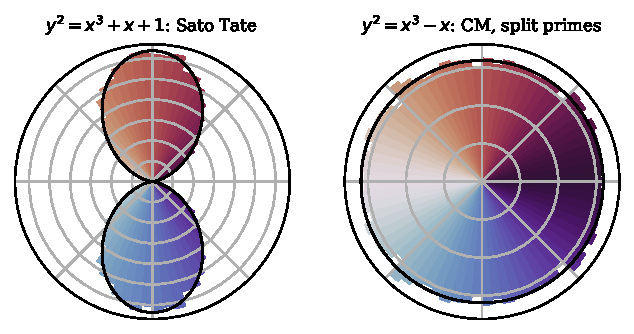
\includegraphics[width=0.92\textwidth]{figs/frobenius_roses.pdf}
\caption{Polar histograms of the Frobenius angles $\pm\theta_p$ for the primes below $4\times10^5$; the radius is the density, the radial labels are omitted, and each panel has its own radial scale. Left: $E_1$, with the Sato Tate density $\sin^2\theta/\pi$ (black). Right: $E_2$, split primes only, with the uniform density $1/(2\pi)$ (black); the inert primes, where $\theta_p = \pi/2$, are omitted.}\label{fig:04roses}
\end{figure}

\section{Complex multiplication and the Weyl fingerprint}\label{sec:04cm}

Suppose now that $E$ has complex multiplication by an order in an imaginary quadratic field $M$. Deuring \cite{deuring1953} showed that $L(s,E) = L(s,\psi)$ for a Hecke Gr\"ossencharacter\index{Hecke Gr\"ossencharacter} $\psi$ of $M$ of infinity type $(1,0)$. For a prime $p \nmid N$ inert in $M$ the curve is supersingular and $a_p = 0$. For $p$ split, $p = \mathfrak p\bar{\mathfrak p}$, we have $a_p = \psi(\mathfrak p) + \overline{\psi(\mathfrak p)}$, and the argument of $\psi(\mathfrak p)/\sqrt p$ is $\pm\theta_p$. Hecke proved \cite{hecke1918} that these angles are equidistributed on the circle. In the language of this chapter, the Weyl criterion on $\mathrm{U}(1)$ applies because the $L$ functions of the unitary characters $(\psi/|\psi|)^n$, $n \ne 0$, are entire and nonvanishing on $\Re s = 1$. By the Chebotarev density theorem half the primes split. Combining these, $(x_p)$ is equidistributed with respect to
\[
\mu_{\mathrm{CM}}(dx) = \frac12\delta_0(dx) + \frac12\,\frac{dx}{\pi\sqrt{4-x^2}}, \qquad x\in[-2,2],
\]
a point mass at $0$ plus an arcsine law. Group theoretically, $\mu_{\mathrm{CM}}$ is the image of Haar measure on the normaliser $N(\mathrm{U}(1))$ of the diagonal torus in $\SU(2)$: the identity component contributes the arcsine law, since a uniform angle $\theta$ gives $2\cos\theta$ arcsine distributed, and the other component consists of elements of trace $0$. The moments are $\int x^{2m}\,d\mu_{\mathrm{CM}} = \frac12\binom{2m}{m}$ for $m \ge 1$.

\begin{proposition}[Weyl fingerprint of the CM law]\label{prop:04cm}
For $n \ge 1$,
\[
\int_{-2}^2 U_n(x/2)\,\mu_{\mathrm{CM}}(dx) = \begin{cases} 1 & 4 \mid n,\\ 0 & \text{otherwise.}\end{cases}
\]
\end{proposition}

\begin{proof}
Under the arcsine law the angle $\theta$ is uniform on $[0,\pi]$, so the continuous part contributes
\[
\frac1\pi\int_0^\pi \frac{\sin((n+1)\theta)}{\sin\theta}\,d\theta = \frac1\pi\int_0^\pi\sum_{j=0}^n e^{i(n-2j)\theta}\,d\theta .
\]
Pairing the terms $j$ and $n-j$ writes the sum as $1$ (present only for $n$ even, from $j = n/2$) plus terms $2\cos((n-2j)\theta)$ with $n - 2j \ne 0$, each of which integrates to $0$ over $[0,\pi]$. So the arcsine average of $U_n(x/2)$ is $1$ for $n$ even and $0$ for $n$ odd. At the atom, $U_n(0) = \sin((n+1)\pi/2) = \cos(n\pi/2)$, which is $0$ for $n$ odd and $(-1)^{n/2}$ for $n$ even. Averaging the two halves gives $0$ for $n$ odd and $\frac12(1 + (-1)^{n/2})$ for $n$ even, which is $1$ when $4\mid n$ and $0$ when $n \equiv 2 \pmod 4$.
\end{proof}

As predicted by the remark after Theorem~\ref{thm:04weyl}, this is the dimension of the $N(\mathrm{U}(1))$ invariants in $\Sym^n$: the torus fixes only the weight zero vector (for $n$ even), and the other component acts on it by $(-1)^{n/2}$.

Figure~\ref{fig:04weyl} shows the fingerprint in our data. For $E_2: y^2 = x^3 - x$ (conductor $32$) and the good primes below $10^7$, the averages at $n = 4, 8, 12$ are $0.9995$, $0.9988$, $0.9979$, and the other averages with $n \le 12$ lie within $0.0018$ of zero. The proportion of these primes with $a_p = 0$ is $0.5002$. The even moments of $x_p$ for $E_2$ are within $0.14\%$ of $\frac12\binom{2m}{m}$ (Table~\ref{tab:05moments}).

\begin{figure}[t]\centering
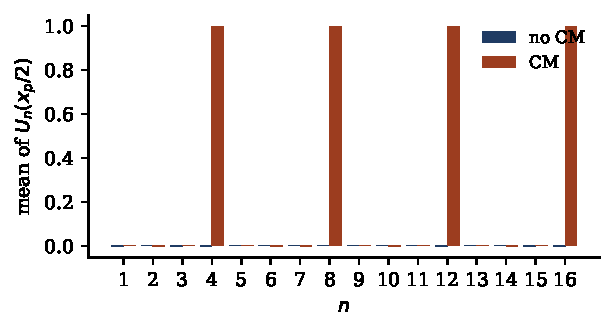
\includegraphics[width=0.8\textwidth]{figs/weyl.pdf}
\caption{Weyl averages $\pi(x)^{-1}\sum_{p\le x}U_n(x_p/2)$ for $1 \le n \le 16$ over the good primes below $10^7$. For $E_1$ (no CM, left bar of each pair) they are close to $0$, the limit that Theorem~\ref{thm:04weyl} requires of a sequence equidistributed for $\ST$; for the CM curve $E_2$ (right bar) they are close to $1$ when $4 \mid n$ and to $0$ otherwise, the limits of Proposition~\ref{prop:04cm}.}\label{fig:04weyl}
\end{figure}

Chapter~\ref{ch:12} turns this separation into a sequential Bayesian test with explicit error exponents.

\section{Joint Sato Tate and coincidences}

For two curves, the pairs $(\theta_p(E), \theta_p(E'))$ are classes in $\SU(2)\times\SU(2)$, whose irreducible representations are $\Sym^m\boxtimes\Sym^n$. By Theorem~\ref{thm:04weyl}, joint equidistribution with respect to $\ST\otimes\ST$ is equivalent to
\[
\frac{1}{\pi(x)}\sum_{p\le x}U_m(x_p/2)\,U_n(x'_p/2) \to 0 \qquad\text{for all } (m,n)\ne(0,0).
\]
By the argument of Theorem~\ref{thm:04serre}, with $(m+1)(n+1)$ in place of $n+1$, this follows if for each $(m,n)\ne(0,0)$ the Rankin Selberg $L$ function $L(s,\Sym^m E\times\Sym^n E')$, with Euler factors
\[
\prod_{i=0}^{m}\prod_{j=0}^{n}\bigl(1-\alpha_p^i\beta_p^{m-i}\alpha_p'^{\,j}\beta_p'^{\,n-j}p^{-s}\bigr)^{-1}
\]
at the primes $p$ of good reduction for both curves (the factors at the finitely many other primes are holomorphic and nonvanishing on $\Re s > 0$, as for a single curve), extends holomorphically to a neighbourhood of $\Re s\ge1$ and has no zeros on $\Re s = 1$. Isogenous curves have equal traces, and a quadratic twist by $\chi$ has $a_p(E') = \chi(p)a_p(E)$, which puts the pairs on the lines $x' = \pm x$; so the right hypothesis is that $E$ and $E'$ are not isogenous over $\bar\Q$.

\begin{theorem}[Joint Sato Tate; Harris \cite{harris2009}]\label{thm:04joint}
Let $E$ and $E'$ be elliptic curves over $\Q$ without complex multiplication that are not isogenous over $\bar\Q$. Then the pairs $(x_p(E), x_p(E'))$ are equidistributed in $[-2,2]^2$ with respect to $\ST\otimes\ST$.
\end{theorem}

Harris \cite{harris2009} reduced the theorem to the potential automorphy of the symmetric powers of $E$ and $E'$ over a common totally real field, and proved it assuming results on the Galois representations attached to automorphic representations of unitary groups that were then expected; those results were established soon afterwards (see the introduction of \cite{blght2011}). Given the automorphy of all symmetric powers \cite{newtonthorne2021,newtonthorne2021b}, the theorem also follows directly from Rankin Selberg theory. For unitary cuspidal automorphic representations $\Pi$ and $\Pi'$, the $L$ function $L(s,\Pi\times\Pi')$ has no zeros on $\Re s = 1$ \cite{shahidi1981}, and it is holomorphic on $\Re s \ge 1$ unless $\Pi' \cong \tilde\Pi\otimes|\det|^{it}$ for some real $t$, in which case its only pole there is a simple pole at $s = 1 - it$ \cite{jpss1983,jacquetshalika1981,moeglinwaldspurger1989}.

For $(m,n)\ne(0,0)$ the hypothesis excludes this exceptional isomorphism when $\Pi$ and $\Pi'$ are the cuspidal automorphic representations attached to $\Sym^m E$ and $\Sym^n E'$, by an argument of Harris that rests on Faltings' isogeny theorem \cite{faltings1983}. Both have trivial central character (symmetric powers of $\SU(2)$ have determinant $1$), while $\tilde\Pi\otimes|\det|^{it}$ has central character $|\cdot|^{it(m+1)}$, so $t = 0$, and the dimensions give $m = n$. Then $\Sym^n\rho_{E,\ell}\cong\Sym^n\rho_{E',\ell}$ for the $\ell$ adic representations on the Tate modules (Chapter~\ref{ch:03}), which, as their images are open in $\GL_2(\Z_\ell)$ (Theorem~\ref{thm:ch3serre}), makes the adjoint representations agree and so forces $\rho_{E',\ell}\cong\rho_{E,\ell}\otimes\eta$ for a character $\eta$, quadratic because both determinants are the cyclotomic character. By Faltings' theorem $E'$ is then isogenous to a quadratic twist of $E$, hence to $E$ over an extension of $\Q$ of degree at most $2$. For curves over $\Q$ without complex multiplication an isogeny over $\bar\Q$ is already defined over such an extension, so our hypothesis is equivalent to Harris's, that $E$ and $E'$ do not become isogenous over an abelian extension of $\Q$.

\begin{corollary}\label{cor:04coinc}
Under the hypotheses of Theorem~\ref{thm:04joint}, the set of primes $p$ with $a_p(E) = a_p(E')$ has natural density zero.
\end{corollary}

\begin{proof}
If $a_p(E) = a_p(E')$ then $x_p = x'_p$, so $(x_p, x'_p)$ lies on the diagonal $\Delta = \{(u,u) : u \in [-2,2]\}$. The set $\Delta$ is closed, and $(\ST\otimes\ST)(\Delta) = \int \ST(\{u\})\,\ST(du) = 0$ because $\ST$ has no atoms. The portmanteau theorem and Theorem~\ref{thm:04joint} give
\[
\limsup_{x\to\infty}\frac{\#\{p\le x: a_p(E) = a_p(E')\}}{\pi(x)} \le (\ST\otimes\ST)(\Delta) = 0. \qedhere
\]
\end{proof}

The heuristic behind the Lang Trotter conjecture (Chapter~\ref{ch:05}) predicts the size of this set. If $a_p(E)$ and $a_p(E')$ were independent integers distributed like $\sqrt p$ times Sato Tate variables, they would agree with probability about $p^{-1/2}\int_{-2}^2 \bigl(\sqrt{4-u^2}/(2\pi)\bigr)^2\,du = \frac{8}{3\pi^2}\,p^{-1/2}$, so the number of coincidences up to $x$ should be of order $\sqrt x/\log x$, with a constant that also reflects congruences between the two curves.

\section{The general Sato Tate conjecture}

By Theorem~\ref{thm:04weyl} and Serre's argument, the general Sato Tate conjecture for an abelian variety $A/\Q$ (Conjecture~\ref{conj:ch3gst}, with $\mathrm{ST}(A)$ as in Definition~\ref{def:ch3stgroup}) follows if the $L$ functions attached to the nontrivial irreducible representations of $\mathrm{ST}(A)$ extend holomorphically to a neighbourhood of $\Re s \ge 1$ without zeros on $\Re s = 1$, a consequence of the Langlands conjectures. For the $52$ groups of abelian surfaces (Theorem~\ref{thm:ch3fkrs}), the moment statistics of the curves that Fit\'e, Kedlaya, Rotger and Sutherland \cite{fkrs2012} exhibit for each group, integer combinations of values of the Weyl fingerprint, match the predicted ones numerically; the conjecture is open for $\mathrm{ST}(A)=\USp(4)$ and known in many other cases, as recorded after that theorem.

\section{Notes}

Weyl's paper \cite{weyl1916} contains the criterion and the equidistribution of polynomial sequences by differencing. The appendix to Chapter I of Serre's book \cite{serre1968} is the standard reference for the compact group version and the source of Theorem~\ref{thm:04serre}. Sato found the $\sin^2$ law numerically; Tate derived it from the expectation that algebraic cycles on powers of $E$ account for the poles of symmetric power zeta functions \cite{tate1965}. Birch \cite{birch1968} proved a vertical version: averaged over all elliptic curves over $\mathbb{F}_p$, the even moments of $a_p/\sqrt p$ tend to the Catalan numbers as $p\to\infty$. Chapter~\ref{ch:06} surveys such vertical laws, and Chapter~\ref{ch:07} treats the one for Hecke eigenvalues.

The route through potential automorphy is surveyed in the introductions of \cite{hsbt2010,blght2011}; the tensor product device of Harris \cite{harris2009} is one of the ingredients of \cite{blght2011}. Newton and Thorne's proof \cite{newtonthorne2021,newtonthorne2021b} combines automorphy lifting with an analytic continuation argument along the Coleman Mazur eigencurve, and Thorner \cite{thorner2021} used their theorem to prove effective forms of Sato Tate. Serre's lecture notes \cite{serre2012} give the general formalism, Sutherland's survey \cite{sutherland2019} describes Sato Tate groups and their moment sequences, and the database \cite{lmfdb} records Sato Tate groups of many curves and abelian surfaces. Katz and Sarnak \cite{katzsarnak1999} develop the analogous theory over finite fields, where Deligne's equidistribution theorem \cite{deligne1980} proves the analogue of the conjecture for families.

Nothing in this chapter proves functoriality: Theorem~\ref{thm:04serre} derives a probabilistic consequence, and the arithmetic input of Theorem~\ref{thm:04STthm} was supplied by others. Proposition~\ref{prop:01limits} records the converse limitation: no statistic of the empirical law of $(x_p)$ alone can detect automorphy.

\section{Exercises}

\begin{enumerate}
\item Show that the irreducible characters of $\mathrm{U}(1)$ are $\theta \mapsto e^{ih\theta}$, $h\in\Z$, and deduce from Theorem~\ref{thm:04weyl}, in the form for sequences indexed by the integers noted after its proof, Weyl's theorem that $(n\alpha \bmod 1)$ is equidistributed for irrational $\alpha$. Show that the same sequence is not equidistributed for any rational $\alpha$ by exhibiting a Weyl average that does not tend to zero.
\item Prove that the arcsine law $dx/(\pi\sqrt{4-x^2})$ on $[-2,2]$ has even moments $\binom{2m}{m}$, by counting all (not only nonnegative) paths of $\pm1$ steps that return to $0$. Deduce the moments of $\mu_{\mathrm{CM}}$, and compare with the Catalan numbers by the ballot theorem.
\item Let $E/\Q$ be an elliptic curve without complex multiplication, and let $g$ be a Riemann integrable function on $[-2,2]$. Show that $\pi(x)^{-1}\sum_{p\le x}g(x_p)$ tends to $\int g\,d\ST$ (approximate $g$ from above and below by continuous functions), and deduce that the primes with $|a_p| \le \sqrt p$ have natural density $\frac13 + \frac{\sqrt3}{2\pi}$.
\item Let $H \subset \SU(2)$ be a finite subgroup and $\mu$ the image on $[-2,2]$, under the trace, of the uniform probability measure on $H$. Show that $\int U_n(x/2)\,\mu(dx)$ is a nonnegative integer for every $n$, and that it is at least $1$ whenever $n$ is a multiple of $2|H|$. Conclude that no such $\mu$ can be the limiting law of $(x_p)$ for a newform without complex multiplication.
\item\label{ex:04clt} (Probabilistic.) Let $Y_1, Y_2, \dots$ be independent with law $\ST$, and $W_n(T) = T^{-1}\sum_{j\le T}U_n(Y_j/2)$. Show that for every finite set $S$ of positive integers the vector $(\sqrt T\,W_n(T))_{n\in S}$ converges in law as $T\to\infty$ to a vector of independent standard normal variables. What changes when the $Y_j$ have law $\mu_{\mathrm{CM}}$? Compute the means and covariances of the $U_n(Y_j/2)$ in that case.
\end{enumerate}

\section{Open computational problems}

\begin{compproblem}[Weyl averages at scale]
Objective: measure how fast the Weyl averages $W_n(x) = \pi(x)^{-1}\sum_{p\le x}U_n(x_p/2)$ tend to zero, and how the rate depends on $n$, for $E_1$ and for the $200$ random curves of Chapter~\ref{ch:05}, for $1 \le n \le 50$ and all primes up to $10^{10}$ (about $4.6\times10^8$ primes per curve). Route: PARI/GP \texttt{ellap} over blocks of primes in parallel, GPU baby step giant step, or Harvey's average polynomial time algorithm \cite{harvey2014}, accumulating $U_n(x_p/2)$ for all $n \le 50$ by the three term recurrence. Deliverable: plots on logarithmic axes of $\sqrt{\pi(x)}\,|W_n(x)|$ against $x$ and $n$, with a fitted law for its growth in $n$. Why it matters: for independent draws from $\ST$ the quantity $\sqrt{\pi(x)}\,W_n(x)$ is asymptotically standard normal for every $n$ (Exercise~\ref{ex:04clt}), while the generalized Riemann hypothesis for $L(s,\Sym^n E)$ gives, through the explicit formula, only $W_n(x) = O(n\,x^{-1/2}\log x\,\log(nNx))$ with $N$ the conductor of $E$ (Chapter 5 of \cite{iwanieckowalski2004}); the data show which of the two describes the dependence on $n$.
\end{compproblem}

\begin{compproblem}[Fingerprints of genus two Jacobians]
Objective: compute the exact Weyl fingerprints of the $52$ Sato Tate groups $G$ of abelian surfaces \cite{fkrs2012}, that is the integers $\int\chi_\rho\,d\mu_G = \dim\rho^G$ for all irreducible representations $\rho$ of $\USp(4)$ with highest weight $(a,b)$, $a \ge b \ge 0$, $a + b \le 12$; find a smallest set of such $\rho$ that separates the $52$ groups, or the pairs that this range cannot separate; and compare the fingerprints with the empirical Weyl averages of the $66{,}158$ genus two curves in the LMFDB (absolute discriminant at most $10^6$), using all primes up to $10^8$. Route: branching from $\USp(4)$ to the identity component of $G$, followed by the action of the component group, in Sage or Magma; $L$ polynomials by the methods of \cite{kedlayasutherland2009} or by the average polynomial time algorithm of \cite{harveysutherland2014}. Deliverable: the table of fingerprints, a minimal separating set of representations, and for each curve the empirical averages on that set with the group they single out. Why it matters: Weyl averages are sufficient in the limit for the Bayesian identification of Chapter~\ref{ch:12}, so a minimal separating set measures how few averages identify a Sato Tate group; agreement for each group that occurs among these curves tests the general Sato Tate conjecture group by group, including groups for which it is not known.
\end{compproblem}

\begin{compproblem}[Joint laws of pairs and twists]
Objective: count the coincidences of Corollary~\ref{cor:04coinc}, and contrast the joint laws of unrelated pairs with those of twists. Problem~3.3 already tests the independence of unrelated pairs, with twists as a control, by joint Weyl averages and discrepancy; here the focus is the density zero set of coincidences. Objects: $10^3$ pairs of curves of conductor below $10^4$ without complex multiplication that are not isogenous over $\bar\Q$, and $E_1$ with its quadratic twists by the fundamental discriminants $d \ne 1$ with $|d| \le 10^3$; all primes up to $10^9$. Route: LMFDB curve lists and PARI/GP \texttt{ellap} in batch; a twist has traces $\chi_d(p)\,a_p(E_1)$ and needs no new point counts. Deliverable: for the unrelated pairs, the counts $\#\{p\le x : a_p(E) = a_p(E')\}$ at $x = 10^6,\dots,10^9$ fitted to $c\sqrt x/\log x$ and compared with $c_0 = 16/(3\pi^2) \approx 0.54$, the value for independent Sato Tate traces, corrected for congruences from the mod $\ell$ images as Lang and Trotter do for $a_p = 0$; and heat maps of the joint Weyl averages $\pi(x)^{-1}\sum_{p\le x}U_m(x_p/2)U_n(x'_p/2)$, $m,n \le 10$, whose limits are $0$ for unrelated pairs when $(m,n)\ne(0,0)$, and for twists $\delta_{mn}$ for even $n$ and $0$ for odd $n$. Why it matters: Corollary~\ref{cor:04coinc} gives only density zero; the constants $c$ are the analogue for pairs of the Lang Trotter constants of Chapter~\ref{ch:05}, and quadratic twists, up to isogeny over $\Q$, are exactly the pairs excluded from Theorem~\ref{thm:04joint}.
\end{compproblem}


\chapter{Frobenius Data: Statistics at Scale}\label{ch:05}

Sato did not derive the semicircle; he saw it, in point counts of specific curves modulo many primes. Birch and Swinnerton Dyer, at about the same time, found their conjecture in plots of $\log\prod_{p\le x}N_p/p$, with $N_p = \#E(\mathbb{F}_p)$, against $\log\log x$, computed on the EDSAC 2 computer in Cambridge \cite{bsd1965}. Both were statistical observations before they were theorems or programmes. This chapter treats Frobenius data in the same spirit and asks three questions of it. How fast does the empirical law approach the Sato Tate law? What correction at the scale of $\log x$ encodes the rank? How often does a trace take a prescribed value? The first leads to discrepancy, the second to the explicit formula, the third to the Lang Trotter conjecture. For each we state what is proved, what is conjectured, and what our computations show, keeping the distance between a stable statistic and a theorem in view.

\section{Computing traces of Frobenius}

Let $E: y^2 = x^3 + ax + b$ with $a,b\in\Z$ and discriminant $\Delta = -16(4a^3+27b^2) \ne 0$. For a prime $p \nmid 2\Delta$ we have
\[
a_p = p + 1 - \#E(\mathbb{F}_p) = -\sum_{x\in\mathbb{F}_p}\Bigl(\frac{x^3+ax+b}{p}\Bigr),
\]
since each $x$ contributes $1 + \bigl(\frac{x^3+ax+b}{p}\bigr)$ affine points and there is one point at infinity. This gives an $O(p)$ algorithm, adequate for $p$ up to about $10^5$ and convenient for checking.\index{point counting}

Baby step giant step methods reduce the cost to $O(p^{1/4})$ group operations: by Hasse, $\#E(\mathbb{F}_p)$ lies in an interval of length $4\sqrt p$, and one searches it for a multiple $m$ of the order of a random point; Mestre's trick with the quadratic twist makes the answer unique for $p > 229$. Schoof's algorithm \cite{schoof1985} computes $a_p \bmod \ell$ from the action of Frobenius on $\ell$ torsion and recovers $a_p$ by the Chinese remainder theorem in time polynomial in $\log p$; the Elkies and Atkin improvements (SEA) are the method of choice at cryptographic sizes. PARI/GP \cite{pari2023} chooses among these in \texttt{ellap}.

For all primes up to a bound the cost per prime is tiny: the $664{,}577$ traces of $E_1$ below $10^7$ took about $20$ seconds on one core. For much larger ranges Harvey's average polynomial time method \cite{harvey2014} computes $a_p$ for all $p\le X$ at once, at a cost per prime polynomial in $\log X$.

\section{The data sets of this book}

All computations were carried out for this book with PARI/GP and Python, on these data.

\begin{enumerate}
\item $E_1: y^2 = x^3 + x + 1$, discriminant $-496$, conductor $496 = 2^4\cdot31$ (LMFDB label 496.a1 \cite{lmfdb}), without complex multiplication; all $664{,}577$ good primes below $10^7$.
\item $E_2: y^2 = x^3 - x$, complex multiplication by $\Z[i]$, conductor $32$; all good primes below $10^7$.
\item Ramanujan's $\tau(p)/p^{11/2}$ for the $78{,}498$ primes below $10^6$.
\item Two hundred curves $y^2 = x^3 + ax + b$ with integers $a,b$ drawn uniformly from $[-50,50]$ (four curves occur twice), singular curves and curves with complex multiplication being discarded; all good primes $p$ with $5\le p<10^6$, about $7.8\times10^4$ per curve.
\item The curves $11a1$, $37a1$, $389a1$ and $5077a1$ of the Cremona tables, of rank $0$, $1$, $2$ and $3$ (the smallest conductors of these ranks); all odd primes below $10^7$.
\end{enumerate}

Table~\ref{tab:05moments} shows the even moments of the normalised traces. They agree with the Catalan numbers $C_m$ (for $E_1$ and $\tau$) and with the moments $\frac12\binom{2m}{m}$ of the CM law $\mu_{\mathrm{CM}}$ of Section~\ref{sec:04cm} (for $E_2$) to relative errors at most $0.06\%$, $0.73\%$ and $0.14\%$ respectively, in every case within one standard error of the corresponding average of independent draws. For $\tau$, Deligne's bound is visible directly: the largest value of $|\tau(p)|/p^{11/2}$ below $10^6$ is $1.99920$.

\begin{table}[t]\centering\small
\begin{tabular}{rrrrrr}
\toprule
$2m$ & $E_1$ & $\tau$ & $C_m$ & $E_2$ & $\frac12\binom{2m}{m}$\\
\midrule
2 & 1.0000 & 0.9987 & 1 & 0.9995 & 1\\
4 & 1.9994 & 1.9939 & 2 & 2.9980 & 3\\
6 & 4.9976 & 4.9772 & 5 & 9.9916 & 10\\
8 & 13.9930 & 13.9204 & 14 & 34.9642 & 35\\
10 & 41.9808 & 41.7250 & 42 & 125.8514 & 126\\
12 & 131.9488 & 131.0436 & 132 & 461.3908 & 462\\
\bottomrule
\end{tabular}
\caption{Even moments of normalised traces: $E_1$ and $E_2$ over good primes below $10^7$, $\tau(p)/p^{11/2}$ over primes below $10^6$, against the Sato Tate (Catalan) and CM predictions.}\label{tab:05moments}
\end{table}

Write $W_j$ for the Weyl average of $U_j(x_p/2)$ over the good primes $p\le x$ (Chapter~\ref{ch:04}). Since $x^{2m} = \sum_{k=0}^m b_{m,k}U_{2k}(x/2)$ with $b_{m,k} = \binom{2m}{m-k} - \binom{2m}{m-k-1}\ge0$ and $b_{m,0} = C_m$, the $2m$th moment equals $C_m + \sum_{k=1}^m b_{m,k}W_{2k}$. The coefficients sum to $\binom{2m}{m}\sim4^m/\sqrt{\pi m}$, so high moments amplify small errors; for questions of rate the right object is the distribution function.

\section{Discrepancy}\label{sec:05disc}

Let $F_{\mathrm{ST}}(t) = \ST([-2,t])$ and let $F_n$ be the empirical distribution function of the first $n$ normalised traces $x_{p_1},\dots,x_{p_n}$, where $p_1<p_2<\cdots$ are the good primes. The \emph{Kolmogorov discrepancy}\index{discrepancy} is
\[
D_n = \sup_{t\in[-2,2]}\bigl|F_n(t) - F_{\mathrm{ST}}(t)\bigr| .
\]
By Theorem~\ref{thm:04STthm} and the continuity of $F_{\mathrm{ST}}$, $D_n\to0$ for every curve without complex multiplication. The question is the rate.

The classical link between $D_n$ and Weyl sums is the inequality of Erd\H{o}s and Tur\'an \cite{erdosturan1948}.\index{Erd\H{o}s Tur\'an inequality}

\begin{theorem}[Erd\H{o}s and Tur\'an]
There is an absolute constant $C$ such that for any points $u_1,\dots,u_n$ in $\R/\Z$ and any integer $M\ge1$,
\[
\sup_{I}\Bigl|\frac{\#\{j\le n: u_j\in I\}}{n} - |I|\Bigr| \le C\Bigl(\frac{1}{M} + \sum_{h=1}^M \frac1h\Bigl|\frac1n\sum_{j=1}^n e^{2\pi i h u_j}\Bigr|\Bigr),
\]
the supremum being over intervals $I$.
\end{theorem}

An analogue for the Sato Tate measure, with Weyl averages of Chebyshev polynomials $U_m$ in place of exponential sums, was proved by Niederreiter \cite{niederreiter1991}. Combined with bounds for Weyl averages from the analytic properties of $L(s,\Sym^m E)$, it converts zero free regions into rates for $D_n$. In the opposite direction, sharp rates for $D_n$ constrain the zeros.

\begin{theorem}[Akiyama and Tanigawa \cite{akiyamatanigawa1999}; Mazur \cite{mazur2008}]
Let $E/\Q$ be an elliptic curve without complex multiplication. If $D_n = O(n^{-1/2+\varepsilon})$ for every $\varepsilon > 0$, then the Riemann hypothesis holds for $L(s,\Sym^m E)$ for every $m\ge1$.
\end{theorem}

Akiyama and Tanigawa conjectured the rate in the hypothesis and proved the case $m = 1$, the Riemann hypothesis for $L(s,E)$. The extension to all $m$ is stated by Mazur under analytic hypotheses on $L(s,\Sym^mE)$ that the theorem of Newton and Thorne \cite{newtonthorne2021,newtonthorne2021b} now supplies (Chapter~\ref{ch:04}). The argument is short. The function $U_m(x/2)$ has bounded variation on $[-2,2]$ and Sato Tate mean zero, so integration by parts gives $|\sum_{j\le n}U_m(x_{p_j}/2)|\le V_m\,nD_n$, with $V_m$ its total variation, and the hypothesis gives $\sum_{p\le x}U_m(x_p/2)\ll x^{1/2+\varepsilon}$. In the unitary normalisation, with centre $s = \frac12$, partial summation shows that $\sum_pU_m(x_p/2)p^{-s}$ converges on $\Re s>\frac12+\varepsilon$, while the prime powers and the bad primes contribute a function holomorphic on $\Re s>\frac12$. Hence $\log L(s,\Sym^mE)$ continues holomorphically to $\Re s>\frac12+\varepsilon$, and $L(s,\Sym^mE)$ has no zeros there (Exercise~3); since $\varepsilon$ is arbitrary, the functional equation does the rest. Results in the other direction are much weaker. Using the functoriality of Newton and Thorne, Thorner \cite{thorner2021} proved unconditionally that $D_n\ll\log(N\log p_n)/\sqrt{\log p_n}$, with $N$ the conductor of $E$ and an absolute implied constant. For squarefree $N$ and assuming the Riemann hypothesis for every $L(s,\Sym^mE)$, Rouse and Thorner \cite{rousethorner2017} obtained the explicit form $D_n\ll p_n^{-1/4}\log(Np_n)$ of V. K. Murty's bound \cite{murty1985} of order $n^{-1/4}$ up to logarithms, still far from $n^{-1/2}$.

\begin{figure}[t]\centering
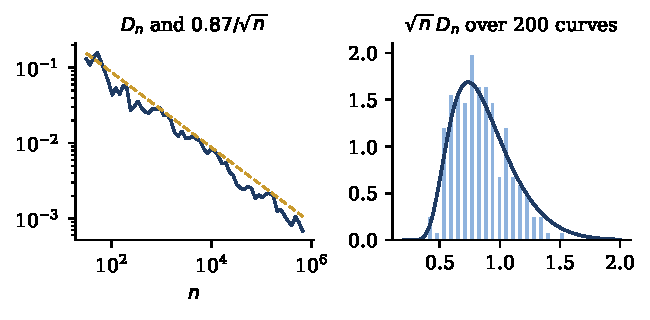
\includegraphics[width=\textwidth]{figs/discrepancy.pdf}
\caption{Left: Kolmogorov discrepancy $D_n$ for $E_1$ against $0.87/\sqrt n$, the asymptotic mean of $D_n$ for $n$ independent draws from $\ST$. Right: histogram of $\sqrt n\,D_n$ over $200$ random curves without complex multiplication (primes below $10^6$) against the density of the Kolmogorov distribution.}\label{fig:05discrepancy}
\end{figure}

\subsection{Our evidence}

For $E_1$ the scaled discrepancy $\sqrt n\,D_n$ equals $0.60$, $0.79$, $0.80$, $0.66$, $0.55$ at $n = 10^2, 10^3, 10^4, 10^5$ and at $n = 664{,}577$ (all good primes below $10^7$). The values stay of order one over almost four orders of magnitude (Figure~\ref{fig:05discrepancy}), as for independent draws; five values of a statistic whose spread under independence is about $0.26$ cannot reveal a slow trend. For $\tau(p)$ over primes below $10^6$ the value is $0.646$.

If the traces were independent draws from $\ST$, Kolmogorov's theorem \cite{kolmogorov1933} would give $\sqrt n\,D_n \Rightarrow K = \sup_{0\le u\le1}|B(u)|$, with $B$ a Brownian bridge (Exercise~2); $K$ has mean $\sqrt{\pi/2}\,\log 2 = 0.8687$, standard deviation $0.2603$, and $10$th, $50$th and $90$th percentiles $0.571$, $0.828$, $1.224$. Over our $200$ random curves, $\sqrt n\,D_n$ has mean $0.837$, standard deviation $0.219$, and percentiles $0.576$, $0.828$, $1.147$. A Kolmogorov Smirnov test of the $200$ values against the law of $K$ gives $p = 0.40$, so it detects no departure from the Kolmogorov law. It has limited power, however, against a contraction of the spread that moves the mean far less than the standard deviation, as here. For $200$ independent copies of $K$ the standard errors of the sample mean and standard deviation are $0.018$ and $0.016$; the observed mean is $1.7$ standard errors below $0.8687$, the standard deviation $2.7$ standard errors below $0.2603$, and the upper tail is visibly lighter (Figure~\ref{fig:05discrepancy}, right). Across curves, the discrepancy at about $7.8\times10^4$ primes has the size expected for independent draws and is, if anything, less dispersed.

\subsection{Interpretation}

Three qualifications apply.

First, the sequence $(x_p)$ is deterministic. A $p$ value of $0.40$ says that a summary of a deterministic object is unremarkable under a reference law; it does not say the object is random. What is random in our experiment is the choice of curve, so the law of $\sqrt n\,D_n$ across curves is a vertical statistic, closer to the family averages of Chapter~\ref{ch:06} than to a statement about one curve.

Second, the explicit formula predicts structure that independent sampling lacks. In the unitary normalisation let $r_m$ be the order of $L(s,\Sym^mE)$ at $s = \frac12$. The prime squares enter through the identity $\tr\Sym^m(g^2) = \sum_{j=0}^m(-1)^j\tr\Sym^{2m-2j}(g)$ (Exercise~4), whose right side has Sato Tate mean $(-1)^m$, and the Riemann hypothesis for $L(s,\Sym^mE)$ gives
\[
\sum_{p\le x}U_m(x_p/2)\log p = -\bigl((-1)^m + 2r_m\bigr)\sqrt x - \sum_{\gamma\ne0}\frac{x^{1/2+i\gamma}}{\frac12+i\gamma} + o(\sqrt x),
\]
with $\gamma$ running over the ordinates of the nontrivial zeros $\frac12+i\gamma$ of $L(s,\Sym^mE)$, counted with multiplicity. By the method of Rubinstein and Sarnak \cite{rubinsteinsarnak1994}, the left side divided by $\sqrt x$ has a limiting distribution in logarithmic scale, with mean $-((-1)^m + 2r_m)$. For $m = 1$, where $r_1 = r$ is the analytic rank of $E$, the mean is $1 - 2r$: this is the rank bias of Section~\ref{sec:05bias}. By partial summation $\sum_{p\le x}U_m(x_p/2)$ is then of order $\sqrt x/\log x$, a factor $\sqrt{\log x}$ below the $\sqrt{\pi(x)}$ of independent sampling. Thus, for each fixed $m$, $\sqrt n\,W_m\to0$ in logarithmic density, $n$ being the number of good primes up to $x$, whereas for independent draws $\sqrt n\,W_m$ is asymptotically standard normal. Since $\sqrt n\,W_m = -\frac12\int_{-2}^2\sqrt n\,(F_n - F_{\mathrm{ST}})(t)\,U_m'(t/2)\,dt$, it follows that under the Riemann hypothesis for every $L(s,\Sym^mE)$ the process $\sqrt n\,(F_n - F_{\mathrm{ST}})$ has no nondegenerate limit in law in logarithmic scale, Brownian bridge or other: every Chebyshev coefficient of a limit would vanish.

The decay is slow, however. The variance of the limiting distribution grows with the logarithm of the analytic conductor of $L(s,\Sym^mE)$, which is at least linear in $m$, and heuristically frequency $m$ is damped only once $\log x$ is large compared with it. Below $10^7$ this can affect only the first few frequencies, consistent with a spread close to that of the Kolmogorov law; whether it accounts for the smaller spread across curves is open. For $E_1$ at $x = 10^7$ the twelve values of $\sqrt n\,W_m$, $m\le12$, have mean square $0.49$ against $1$ for independent draws; a sum of twelve squares of independent standard normal variables falls this low with probability $0.08$, so the data neither confirm nor exclude damping at this scale. The first of them, $-0.36$, may be compared with the leading order prediction $(1-2r)/\sqrt{\log x} = -0.25$ for its mean, $E_1$ having analytic rank $r=1$.

Third, statements at the scale $n^{-1/2}$ are beyond present methods. For independent draws $\sqrt n\,D_n = O(\sqrt{\log\log n})$ almost surely, by the law of the iterated logarithm; for the traces, even $\sqrt n\,D_n = O(n^{\varepsilon})$ for every $\varepsilon>0$ would imply the Riemann hypothesis for every $L(s,\Sym^mE)$, by the theorem above. We state the questions as follows.

\begin{conjecture}[Size of the Sato Tate discrepancy; open]\label{conj:05bridge}
Let $E/\Q$ be without complex multiplication, and let $n$ be the number of good primes up to $x$.
\begin{enumerate}[label=(\alph*)]
\item (Akiyama and Tanigawa.) $D_n = O(n^{-1/2+\varepsilon})$ for every $\varepsilon>0$.
\item $\sqrt n\,D_n\to0$ in logarithmic density: for every $\delta>0$ the set of $x$ with $\sqrt n\,D_n>\delta$ has logarithmic density zero.
\end{enumerate}
\end{conjecture}

Part (b) is our reading of the explicit formula. For each fixed frequency the corresponding statement, $\sqrt n\,W_m\to0$, follows from the Riemann hypothesis for $L(s,\Sym^mE)$, as shown above; the open point is uniformity in $m$, since $D_n$ sees frequencies up to about $\sqrt n$. Part (b) strengthens the conditional statement above that no nondegenerate limit exists along the primes of one curve. Open Problem~\ref{op:disc} of Chapter~\ref{ch:13} asks whether a Brownian bridge arises under another randomisation, for instance over curves of growing conductor, and Computational Problem~\ref{cp:05bridge} proposes a test.

\section{The explicit formula and rank bias}\label{sec:05bias}

Let $E/\Q$ have conductor $N$ and analytic rank $r = \operatorname{ord}_{s=1}L(s,E)$. Write
\[
S(x) = \sum_{p\le x,\ p\nmid N}\frac{a_p\log p}{p} = \sum_{p\le x,\ p\nmid N}\frac{x_p\log p}{\sqrt p}.
\]
For $p\nmid N$ we have $\log(N_p/p) = -a_p/p + (1 - x_p^2/2)/p + O(p^{-3/2})$, and $\sum_{p\nmid N}(x_p^2 - 1)/p$ converges by the prime number theorem for $L(s,\Sym^2E)$; so the asymptotic $\prod_{p\le x}N_p/p\sim A(\log x)^r$ that Birch and Swinnerton Dyer read from their plots \cite{bsd1965} amounts to $\sum_{p\le x,\,p\nmid N}a_p/p = (\frac12 - r)\log\log x + O(1)$. The same prediction with weights $\log p$ is
\[
S(x) \approx \Bigl(\frac12 - r\Bigr)\log x .
\]\index{rank bias}

We explain where the two terms come from. Normalise $L(s,E)$ so that the centre is at $s = 1$ and write $a_p=2\sqrt p\cos\theta_p$. Then
\[
-\frac{L'}{L}(s,E) = \sum_{n}\frac{\Lambda_E(n)}{n^s},\qquad \Lambda_E(p^k) = p^{k/2}\,2\cos(k\theta_p)\log p\quad(p\nmid N).
\]
Assuming the Riemann hypothesis for $L(s,E)$, the explicit formula, applied with a smooth cutoff at the centre, expresses $\sum_{n\le x}\Lambda_E(n)/n$ as $-r\log x$ (the contribution of the zero of order $r$ at $s = 1$) minus a sum over the other zeros $\rho = 1 + i\gamma$, oscillating like $\sum_{\gamma\ne0}x^{i\gamma}/(i\gamma)$, plus a bounded term. The prime terms give $S(x)$. The prime square terms give
\[
\sum_{p\le\sqrt x}\frac{2\cos(2\theta_p)\log p}{p} = \sum_{p\le\sqrt x}\frac{(U_2(x_p/2) - 1)\log p}{p} = -\frac12\log x + o(\log x),
\]
where we used $2\cos2\theta = U_2(\cos\theta) - 1$, Mertens' theorem $\sum_{p\le y}\log p/p = \log y + O(1)$, and the fact that $\sum_{p\le y}U_2(x_p/2)\log p/p = o(\log y)$, which follows from the holomorphy and nonvanishing of $L(s,\Sym^2 E)$ on $\Re s = 1$ in the unitary normalisation (Chapter~\ref{ch:04}). Cubes and higher powers contribute $O(1)$. Hence
\[
S(x) - \frac12\log x = -r\log x - \sum_{\gamma\ne0}\frac{x^{i\gamma}}{i\gamma} + O(1),
\]
heuristically. The $\frac12$ is the shadow of the symmetric square: the prime square coefficient $U_2(x_p/2) - 1$ has average $-1$ over primes because $L(s,\Sym^2E)$ has no pole at $s = 1$. Under the Riemann hypothesis for $L(s,E)$ the oscillatory sum has bounded mean square in $\log x$, so $S(x)/\log x \to \frac12 - r$ in logarithmic mean; a zero off the line would instead produce oscillations of exponential amplitude in $\log x$. The pointwise statement is not known to follow from the Riemann hypothesis, but Kim and Murty \cite{kimmurty2023} showed that if $S(x)/\log x$ has a limit, the limit is $\frac12 - r$. For the product itself, Goldfeld \cite{goldfeld1982} showed that if $\prod_{p\le x}N_p/p\sim A(\log x)^r$ for some $A>0$ and real $r$, where $N_p$ counts the nonsingular points when $p\mid N$, then $L(s,E)$ satisfies the Riemann hypothesis, $r = \operatorname{ord}_{s=1}L(s,E)$, and $A = \sqrt2\,e^{r\gamma_{\mathrm E}}\,r!/L^{(r)}(E,1)$, with $\gamma_{\mathrm E}$ Euler's constant. The factor $\sqrt2$ comes from the same prime squares, which the product cuts off at $p\le x$ rather than at $p^2\le x$; Conrad \cite{conrad2005} relates it to second moments for general $L$ functions. Kuo and Murty \cite{kuomurty2005} and, independently, Conrad showed that the asymptotic for the product is equivalent to $\sum_{n\le x}\Lambda_E(n) = o(x\log x)$, a bound stronger than the $O(x\log^2x)$ that the Riemann hypothesis gives.

\begin{table}[t]\centering\small
\begin{tabular}{lccccc}
\toprule
Curve & $r$ & $\frac12 - r$ & slope & computed $S(10^7)$ & $(\frac12 - r)\log 10^7$\\
\midrule
$11a1$ & 0 & $0.5$ & $0.46$ & $6.46$ & $8.06$\\
$37a1$ & 1 & $-0.5$ & $-0.59$ & $-9.76$ & $-8.06$\\
$389a1$ & 2 & $-1.5$ & $-1.43$ & $-26.73$ & $-24.18$\\
$5077a1$ & 3 & $-2.5$ & $-2.51$ & $-43.54$ & $-40.30$\\
\bottomrule
\end{tabular}
\caption{Rank bias. The slope of $S(x) = \sum_{p\le x}a_p\log p/p$ against $\log x$ is the chord slope $(S(10^7) - S(10^3))/\log 10^4$, compared with $\frac12 - r$. The computed $S$ runs over the odd primes, bad prime included; adding $p = 2$, where $a_2 = -2$ for all four curves, would lower every value of $S$ by $\log 2$ and leave the slopes unchanged.}\label{tab:05bias}
\end{table}

Table~\ref{tab:05bias} and Figure~\ref{fig:05rankbias} show the four curves. The slopes match $\frac12 - r$ to within $0.1$ in every case, and the computed $S(10^7)$ lies below $(\frac12 - r)\log 10^7$ by between $1.6$ and $3.2$, offsets that the explicit formula attributes to the $O(1)$ term and the low lying zeros. The rank is visible with a ruler, and so is the extra $\frac12$.

\begin{figure}[t]\centering
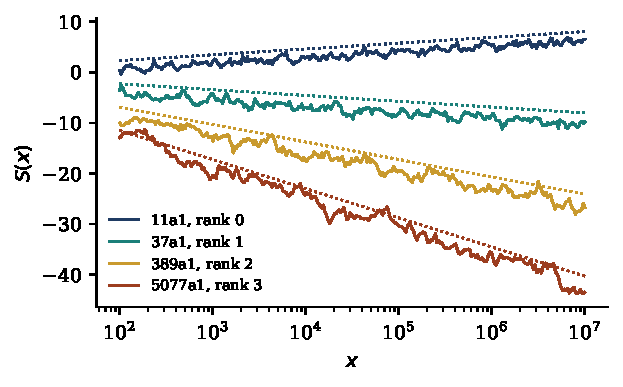
\includegraphics[width=0.85\textwidth]{figs/rankbias.pdf}
\caption{$S(x) = \sum_{p\le x}a_p\log p/p$ for $11a1$, $37a1$, $389a1$, $5077a1$ (ranks $0$ to $3$), $10^2\le x\le 10^7$, summed over odd primes as in Table~\ref{tab:05bias}, against the lines $(\frac12 - r)\log x$.}\label{fig:05rankbias}
\end{figure}

Nothing here bears on the Birch and Swinnerton Dyer conjecture itself: $r$ is the analytic rank, and our data test the explicit formula, not the equality of ranks (known when the analytic rank is at most $1$, by Gross and Zagier \cite{grosszagier1986} and Kolyvagin \cite{kolyvagin1988}).

\section{The Lang Trotter conjecture}

For a fixed integer $t$ let $\pi_{E,t}(x) = \#\{p\le x: p\nmid N,\ a_p = t\}$. When $t = 0$ and $p\ge5$, $a_p = 0$ means that $p$ is a supersingular prime of $E$.\index{Lang Trotter conjecture}\index{supersingular primes}

\begin{conjecture}[Lang and Trotter \cite{langtrotter1976}]
Let $E/\Q$ be without complex multiplication and $t\in\Z$. There is a constant $C_{E,t}\ge0$ such that
\[
\pi_{E,t}(x) \sim C_{E,t}\,\frac{\sqrt x}{\log x},
\]
where for $C_{E,t} = 0$ this means that $\pi_{E,t}(x)$ is bounded.
\end{conjecture}

\subsection{The probabilistic heuristic}

The conjecture concerns a set of primes of density zero, about which Sato Tate says nothing; the heuristic is a local limit version of it. The integer $a_p$ lies in an interval of length $4\sqrt p$, so the lattice spacing is $1$ for $a_p$ and $1/\sqrt p$ for $x_p$. If $x_p$ followed $\ST$ with integrality the only constraint, then
\[
\Prob(a_p = t) \approx \Prob\Bigl(\bigl|x_p - t/\sqrt p\bigr| \le \frac{1}{2\sqrt p}\Bigr) \approx \frac{1}{\sqrt p}\cdot\frac{\sqrt{4 - t^2/p}}{2\pi}\approx \frac{1}{\pi\sqrt p},
\]
since the semicircle density at $0$ is $\frac{1}{2\pi}\cdot2 = \frac1\pi$. Summing over $p$, the expected count is
\[
\sum_{p\le x}\frac{1}{\pi\sqrt p}\approx\frac1\pi\int_2^x\frac{du}{\sqrt u\,\log u} = \frac2\pi\,\pi_{1/2}(x),
\]
where $\pi_{1/2}(x) = \int_2^x du/(2\sqrt u\,\log u)\sim\sqrt x/\log x$, using the prime number theorem in the form that primes near $u$ have density $1/\log u$. This is the shape $c\sqrt x/\log x$ with $c = 2/\pi$.

Congruence conditions correct this. Modulo a prime $\ell$, $a_p$ is the trace of $\Frob_p$ in the mod $\ell$ Galois image $G(\ell)\subset\GL_2(\Z/\ell\Z)$, and by Chebotarev \cite{chebotarev1926} the probability that $a_p\equiv t\pmod\ell$ is $\#\{g\in G(\ell):\tr g = t\}/\#G(\ell)$ rather than $1/\ell$. In the same way the probability that $\ell$ divides $|E(\mathbb F_p)|=p+1-a_p$, the value at $1$ of the characteristic polynomial of $\Frob_p$, is the proportion of elements of $G(\ell)$ with eigenvalue $1$; Koblitz \cite{koblitz1988} built from these proportions his conjecture on the primes $p$ for which $|E(\mathbb F_p)|$ is prime, and Chapter~\ref{ch:flt} reads their complements as the shapes of Gamma laws. By Serre's open image theorem \cite{serre1972} there is an integer $m$ such that the image of Galois in $\GL_2(\hat\Z)$ is the full inverse image of its reduction $G(m)\subset\GL_2(\Z/m\Z)$, and the constant of Lang and Trotter is
\[
C_{E,t} = \frac2\pi\cdot\frac{m\,\#\{g\in G(m):\tr g = t\}}{\#G(m)}\cdot\prod_{\ell\nmid m}\frac{\ell\,\#\{g\in\GL_2(\mathbb{F}_\ell):\tr g = t\}}{\#\GL_2(\mathbb{F}_\ell)}.
\]
The factor at $m$ does not in general split over the primes dividing $m$, because the images modulo different primes can be entangled.

For $t = 0$ and full image $\GL_2(\mathbb{F}_\ell)$ the number of trace zero elements is $\ell^3 - \ell^2$ (Exercise~5), so the factor at $\ell$ is $\ell\cdot\ell^2(\ell-1)/\bigl((\ell^2-1)(\ell^2-\ell)\bigr) = \ell^2/(\ell^2-1)$; for $\ell = 2$ it is $4/3$, as four of the six elements of $\GL_2(\mathbb{F}_2)\cong S_3$ have trace $0$. The mod $2$ image of $E_1$ is all of $\GL_2(\mathbb{F}_2)$, since $x^3+x+1$ is irreducible over $\Q$ with nonsquare discriminant $-31$. If the image of Galois were all of $\GL_2(\hat\Z)$, the constant would be
\[
\frac2\pi\prod_\ell\frac{\ell^2}{\ell^2-1} = \frac2\pi\,\zeta(2) = \frac\pi3\approx1.047.
\]
Over $\Q$ this never happens \cite{serre1972}. For $E_1$ the field $\Q(\sqrt{-31})$ lies in $\Q(E_1[2])$, which contains the square root of the discriminant, and in $\Q(\zeta_{31})\subset\Q(E_1[31])$, so the images modulo $2$ and $31$ are entangled. According to the LMFDB \cite{lmfdb}, $E_1$ is a Serre curve: its image in $\GL_2(\hat\Z)$ has index $2$, the least possible, and is cut out by this single condition. The constant is then a finite computation in $\GL_2(\Z/62\Z)$ (Exercise~5):
\[
C_{E_1,0} = \frac\pi3\Bigl(1 + \frac1{62}\Bigr)\approx1.064.
\]

\subsection{What is known}

The conjecture is open for every curve without complex multiplication and every $t$. Elkies \cite{elkies1987} proved that every elliptic curve over $\Q$ has infinitely many supersingular primes; the lower bounds for $\pi_{E,0}(x)$ that are known are far below $\sqrt x/\log x$. Upper bounds $\pi_{E,t}(x) = O(x^{\theta})$ with $\theta < 1$ follow from effective Chebotarev under the generalized Riemann hypothesis (Serre \cite{serre1981}; Murty, Murty and Saradha \cite{murtymurtysaradha1988}), and averages over families of curves confirm the order $\sqrt x/\log x$ (Fouvry and Murty \cite{fouvrymurty1996} for $t = 0$, David and Pappalardi \cite{davidpappalardi1999} for $t\ne0$). For a curve with complex multiplication half the primes are supersingular, which is why the conjecture excludes such curves.

\subsection{Our counts}

For $E_1$ the supersingular primes begin $3, 17, 179, 227, 523, 1031$. The counts below $x = 10^4, 10^5, 10^6, 10^7$ are $10$, $23$, $79$, $210$, and the ratios $\pi_{E_1,0}(x)/\pi_{1/2}(x)$ are $0.66$, $0.65$, $0.89$, $0.91$ (Figure~\ref{fig:05langtrotter}). At $x = 10^7$, where $\pi_{1/2}(x) = 231.5$, the Poisson standard error of the ratio is $\sqrt{210}/231.5\approx0.06$. The data indicate a constant of order one, above the bare $2/\pi\approx0.64$ and more than two standard errors below $C_{E_1,0}\approx1.064$; the ratio has stayed near $0.9$ since $10^6$. Counts of a few hundred are a consistency check only; Computational Problem~\ref{cp:05lt} asks for counts up to $10^{12}$.

\begin{figure}[t]\centering
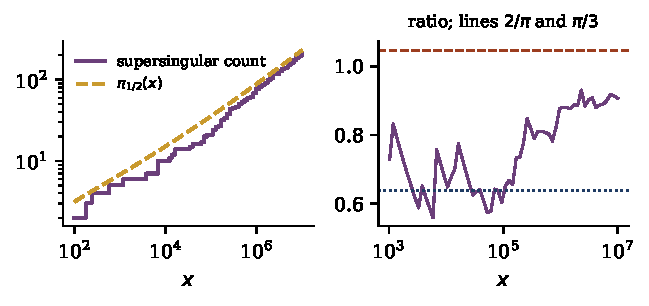
\includegraphics[width=\textwidth]{figs/langtrotter.pdf}
\caption{Supersingular primes of $E_1$ below $10^7$: the count $\pi_{E_1,0}(x)$ against $\pi_{1/2}(x) = \int_2^x du/(2\sqrt u\log u)$ (left), and their ratio (right), with the bare heuristic constant $2/\pi$ and the value $\pi/3$ for a surjective adelic image. The Lang Trotter constant of $E_1$ is $(\pi/3)(1 + 1/62)\approx1.064$.}\label{fig:05langtrotter}
\end{figure}

\section{Notes}

Schoof's algorithm \cite{schoof1985} was the first polynomial time point counting method. Kedlaya and Sutherland \cite{kedlayasutherland2009} computed the distributions of normalised $L$ polynomials of hyperelliptic curves of genus at most $3$ at scale, the numerical side of the classification of Sato Tate groups of abelian surfaces \cite{fkrs2012}. Harvey's average polynomial time method \cite{harvey2014}, made practical by Harvey and Sutherland \cite{harveysutherland2014}, extends such computations much further; Sutherland's survey \cite{sutherland2019} covers the methods, and the LMFDB \cite{lmfdb} holds much of the resulting data. Akiyama and Tanigawa \cite{akiyamatanigawa1999} supported their conjecture with numerical computations of the discrepancy.

The rank bias was implicit in the computations of Birch and Swinnerton Dyer \cite{bsd1965} and made precise by Goldfeld \cite{goldfeld1982}. Sarnak's letter \cite{sarnak2007} treats the biases in the signs of $\tau(p)$ and $a_p$ through all the symmetric powers, and Mazur \cite{mazur2008} discusses the meaning of such error terms. The mechanism is the one behind Chebyshev's bias, where the prime squares produce the bias \cite{rubinsteinsarnak1994}. Chapter~\ref{ch:12} uses the Sato Tate law, with a small atom at $0$ for the supersingular primes, as a likelihood for Bayesian inference.

\section{Exercises}

\begin{enumerate}
\item Prove that $a_p = -\sum_{x\bmod p}\bigl(\frac{x^3+ax+b}{p}\bigr)$ for $p\nmid\Delta$, and deduce that $a_p$ is even if and only if $x^3+ax+b$ has a root modulo $p$. Using the Chebotarev density theorem, compute the proportion of primes with $a_p$ even for $E_1$.
\item Let $Y_1,\dots,Y_n$ be independent with law $\ST$, and let $F_n$ be their empirical distribution function. Show that $\sqrt n\,(F_n - F_{\mathrm{ST}})$ converges in law to $B\circ F_{\mathrm{ST}}$ with $B$ a Brownian bridge, and that $\sqrt n\,D_n\Rightarrow\sup_u|B(u)|$. Verify that $\E\sup_u|B(u)| = \sqrt{\pi/2}\,\log2$.
\item Suppose that $|\sum_{p\le x}U_m(x_p/2)| \le A_m x^{1/2+\varepsilon}$ for all $x\ge2$. Show that the series $\sum_pU_m(x_p/2)p^{-s}$ converges for $\Re s > \frac12+\varepsilon$, and deduce that $L(s,\Sym^mE)$ has no zeros with $\Re s > \frac12 + \varepsilon$ in the unitary normalisation. (Show that the prime powers and the bad primes contribute to $\log L(s,\Sym^mE)$ a function holomorphic on $\Re s>\frac12$.)
\item (Prime squares and bias.) (a) Show that for $g\in\SU(2)$
\[
\tr\Sym^m(g^2) = \sum_{j=0}^m(-1)^j\tr\Sym^{2m-2j}(g),
\]
so that $\tr\Sym^m(g^2)$ has Sato Tate mean $(-1)^m$. (b) Let $x_p$ be independent with law $\ST$. Show that $\sum_{p\le x}x_p\log p/\sqrt p$ has mean $0$ and variance $\sim\frac12\log^2x$, so that a random model without the explicit formula would not produce a drift of size $\frac12\log x$ distinguishable from noise. Explain why the arithmetic sum has much smaller fluctuations.
\item (a) Show that the number of $g\in\GL_2(\mathbb{F}_\ell)$ with trace $t$ is $\ell^3 - \ell^2$ for $t = 0$, and compute it for $t \ne 0$. Deduce the local Lang Trotter factor at $\ell$ for $t\ne0$ when the image is full. (b) Since $E_1$ is a Serre curve, its image in $\GL_2(\hat\Z)$ is the subgroup of index $2$ on which $\operatorname{sgn}(g\bmod2) = \bigl(\frac{\det g}{31}\bigr)$, with $\operatorname{sgn}$ the sign character of $\GL_2(\mathbb{F}_2)\cong S_3$. Show that $C_{E_1,0} = (\pi/3)(1 + e_2e_{31})$, where $e_2$ is the average of $\operatorname{sgn}$ over the trace zero elements of $\GL_2(\mathbb{F}_2)$ and $e_{31}$ that of $\bigl(\frac{\det g}{31}\bigr)$ over the trace zero elements of $\GL_2(\mathbb{F}_{31})$. Show that $e_2 = -\frac12$ and, by counting the solutions of $a^2+bc = -d$, that $e_{31} = -\frac1{31}$, so that $C_{E_1,0} = (\pi/3)(1 + \frac1{62})$.
\item Under the heuristic that the events $\{a_p = 0\}$ are independent with probabilities $C/(2\sqrt p)$, show that $\pi_{E,0}(x)$ has mean and variance both asymptotic to $C\,\pi_{1/2}(x)$ and is asymptotically normal. Using $\pi_{1/2}(10^7) = 231.5$, construct an approximate $95\%$ confidence interval for $C$ from the count $210$ of supersingular primes of $E_1$ below $10^7$, and compare it with $2/\pi$ and with $C_{E_1,0}$.
\end{enumerate}

\section{Open computational problems}

\begin{compproblem}[Brownian bridge test at scale]\label{cp:05bridge}
Objective: test Conjecture~\ref{conj:05bridge}(b) and the predictions for single frequencies in Section~\ref{sec:05disc}, for $E_1$ with all primes up to $10^{10}$ (about $4.6\times10^8$ primes) and for $10^3$ random curves with all primes up to $10^9$. Route: GPU or multicore baby step giant step, or Harvey's average polynomial time algorithm \cite{harvey2014}; streaming accumulation of $F_n$ on a fixed grid and of the Weyl averages $W_m$ for $m\le 100$. Deliverable: plots of $\sqrt n\,D_n$ and of $\sqrt n\,W_m$ against $\log x$, the latter with the means $-((-1)^m + 2r_m)/\sqrt{\log x}$ that the explicit formula predicts; the empirical covariance function of the process at $n = 10^8, 10^9$, compared with $\min(s,t) - st$ after the transform $F_{\mathrm{ST}}$; Kolmogorov Smirnov, Anderson Darling and variance tests of the family values of $\sqrt n\,D_n$ against the law of $K$, with the atom at $0$ created by the supersingular primes treated separately. Why it matters: a decline of $\sqrt n\,D_n$, or of the low frequency Weyl averages, would show the zeros of symmetric power $L$ functions acting on the empirical process and would separate the traces from independent draws; the family test decides whether the smaller spread seen at $10^6$ persists.
\end{compproblem}

\begin{compproblem}[Lang Trotter constants]\label{cp:05lt}
Objective: test the Lang Trotter constants $C_{E,t}$, $t = 0,1,2$, of $E_1$ and of two further Serre curves against counts up to $10^{12}$. Route: adelic images from the LMFDB \cite{lmfdb} and the algorithms of Zywina \cite{zywina2022} and of Rouse, Sutherland and Zureick Brown \cite{rszb2022}; exact evaluation of the Lang Trotter formula by counting in $G(m)$, as in Exercise~5 for $C_{E_1,0}$; counts of $a_p = t$ by testing $(p+1-t)P = O$ for a few random points $P$, much cheaper than computing $a_p$, with hits confirmed by \texttt{ellap}. Deliverable: the constants to six digits; the ratios $\pi_{E,t}(x)/(C_{E,t}\,\pi_{1/2}(x))$ for $x = 10^8,\dots,10^{12}$ with Poisson error bars; a fit of the rate at which they approach $1$. Why it matters: it is the first serious test of the conjecture's constants for these curves, it decides whether the deficit of $E_1$ at $10^7$ is a slow transient, and it measures whether the independence heuristic survives the move from density one statements to density zero ones.
\end{compproblem}

\begin{compproblem}[Bias at high rank]
Objective: check the slope $\frac12 - r$ for curves of rank $4$ to $8$ and beyond, including Elkies's curves of large rank, using all primes below $10^{9}$. Route: curves of rank $4$ to $8$ of small conductor and Elkies's curves, from the LMFDB \cite{lmfdb} and the literature, with $r$ the analytic rank, which for $r\ge4$ is determined only numerically; PARI/GP \texttt{ellap} for the traces; regression of $S(x)$ on $\log x$ with a model for the oscillatory term from the low lying zeros computed by \texttt{lfunzeros} where the conductor permits. Deliverable: a table of fitted slopes against $\frac12 - r$ with confidence bands, and residual plots showing the contribution of the first zeros. Why it matters: for large conductor the oscillatory term is larger and the logarithmic convergence slower, and the data show at what scale the rank becomes legible from Frobenius data alone, a question of practical importance for rank estimation.
\end{compproblem}

\begin{compproblem}[A GPU point counting pipeline]
Objective: build an open pipeline that computes $a_p$ for all primes $p\le10^{10}$ and all curves of conductor up to $10^5$ in the Cremona database, with verification. Route: batched baby step giant step on GPUs with Montgomery arithmetic, cross checked against PARI/GP on random samples and against the Hasse bound and known $L$ values via the approximate functional equation. Deliverable: compressed trace tables, a reproducible build, and timing benchmarks per prime. Why it matters: every statistical question in this chapter and in Chapters~\ref{ch:06} and \ref{ch:12} is limited by data scale, and a shared resource at $10^{10}$ would move discrepancy, bias and Lang Trotter questions into the regime where finite sample effects are small.
\end{compproblem}

\chapter{Random Matrices and Families of L Functions}\label{ch:06}

In spring 1972 Hugh Montgomery visited the Institute for Advanced Study and, over tea, described to Freeman Dyson the function $1-(\sin\pi u/\pi u)^2$ that he had found governing the pair correlation of zeros of the Riemann zeta function. Dyson recognised it at once as the pair correlation of eigenvalues of a random Hermitian matrix from the Gaussian unitary ensemble. That conversation set the agenda for half a century: the conjecture, supported by theorems for restricted test functions and by extensive computation, that zeros of $L$ functions have the local statistics of eigenvalues of random matrices from compact classical groups. This chapter develops the theory, from the Weyl integration formula to the Katz and Sarnak symmetry types, low lying zeros and the Keating and Snaith moment conjectures. Throughout we keep two random matrix limits apart: the Sato Tate limit, in which a fixed compact group of small rank governs Frobenius classes at varying primes, and the Katz and Sarnak limit, in which groups of growing dimension govern the zeros near a fixed point.

\section{Haar measure and the Weyl integration formula}\label{sec:ch6weyl}

Every compact group $K$ carries a unique left and right invariant probability measure, the Haar measure\index{Haar measure} (Chapter~\ref{ch:04}). When $K$ is a connected Lie group, the integral $\int_Kf\,dh$ of a class function $f$ (one constant on conjugacy classes) reduces to an integral over a maximal torus $T$, because every element of $K$ is conjugate into $T$ and two elements of $T$ are conjugate in $K$ precisely when they lie in one orbit of the Weyl group $W=N(T)/T$. The density of the pushforward to $T/W$ is given by Weyl's formula \cite{weyl1925}.\index{Weyl integration formula}

\begin{theorem}[Weyl integration formula]\label{thm:ch6weyl}
Let $K$ be a compact connected Lie group with maximal torus $T$, Weyl group $W$ and set of roots $\Phi$. For every continuous class function $f$,
\[
\int_Kf\,dh=\frac{1}{|W|}\int_Tf(t)\prod_{\alpha\in\Phi}\bigl(1-\alpha(t)\bigr)\,dt ,
\]
where $dt$ is Haar probability measure on $T$.
\end{theorem}

For the unitary group $\mathrm{U}(N)$, with eigenvalues $e^{i\theta_1},\dots,e^{i\theta_N}$, the formula gives the joint density
\[
\frac{1}{(2\pi)^NN!}\prod_{j<k}\bigl|e^{i\theta_j}-e^{i\theta_k}\bigr|^2
\]
on $[0,2\pi)^N$. This is the circular unitary ensemble (CUE). For the compact symplectic group $\USp(2g)$, eigenvalues come in pairs $e^{\pm i\theta_j}$ with $\theta_j\in[0,\pi]$, and the joint density of $(\theta_1,\dots,\theta_g)$ is
\begin{equation}\label{eq:ch6usp}
\frac{2^{g^2}}{g!\,\pi^g}\prod_{j<k}(\cos\theta_j-\cos\theta_k)^2\prod_{j=1}^g\sin^2\theta_j .
\end{equation}
For the even and odd orthogonal groups the factor $\prod\sin^2\theta_j$ is replaced by $1$ and by $\prod\sin^2(\theta_j/2)$, with different constants \cite{katzsarnak1999}. The factor $\prod_{j<k}(\cos\theta_j-\cos\theta_k)^2$, common to the three groups, is eigenvalue repulsion; the single product, which depends on the group, is the interaction with the symmetry point $\theta=0$, and it is this factor that the low lying zeros of Section~\ref{sec:ch6ils} detect. For $\SU(2)=\USp(2)$, Chapter~\ref{ch:04} derives the density from the geometry of the three sphere; here is a proof through Gaussian vectors.

\begin{proposition}\label{prop:ch6su2}
Let $A$ be Haar distributed in $\SU(2)$, with eigenvalues $e^{\pm i\theta}$, $\theta\in[0,\pi]$. Then $\theta$ has density $\frac2\pi\sin^2\theta$, and $x=\tr A=2\cos\theta$ has the semicircle density $\frac{1}{2\pi}\sqrt{4-x^2}$ on $[-2,2]$.
\end{proposition}

\begin{proof}
As in Chapter~\ref{ch:04}, Haar measure on $\SU(2)$ is uniform measure on the unit quaternions $S^3\subset\R^4$ and $\tr A=2u$ with $u$ the first coordinate, so $u$ has the law of $Z_1/(Z_1^2+Z_2^2+Z_3^2+Z_4^2)^{1/2}$ for independent standard Gaussian $Z_j$, and $u^2$ has the Beta$(\frac12,\frac32)$ law. Since $u$ is symmetric, its density is $\frac2\pi\sqrt{1-u^2}$ on $[-1,1]$, and the substitutions $u=\cos\theta$ and $x=2u$ give both claims.
\end{proof}

This agrees with \eqref{eq:ch6usp} for $g=1$. The semicircle is both the Sato Tate law and the Wigner law of large random matrices, but here it is the exact law of the trace of a $2\times2$ matrix. For large $N$, the traces of powers of a Haar unitary matrix are nearly independent Gaussians.

\begin{theorem}[Diaconis and Shahshahani \cite{diaconisshahshahani1994}]\label{thm:ch6ds}
Let $U_N$ be Haar distributed in $\mathrm{U}(N)$ and let $Z_1,Z_2,\dots$ be independent standard complex Gaussian variables, $\E|Z_j|^2=1$. For each fixed $k$,
\[
\bigl(\tr U_N,\tr U_N^2,\dots,\tr U_N^k\bigr)\Rightarrow\bigl(Z_1,\sqrt2\,Z_2,\dots,\sqrt k\,Z_k\bigr)\qquad(N\to\infty).
\]
Moreover, for nonnegative integers $m_j,n_j$ with $N\ge\max(\sum jm_j,\sum jn_j)$, the mixed moments $\E\prod_j(\tr U_N^j)^{m_j}\overline{(\tr U_N^j)}^{n_j}$ equal those of the Gaussian limit exactly, namely $\delta_{m,n}\prod_jj^{m_j}m_j!$.
\end{theorem}

The proof uses power sum symmetric functions and Schur orthogonality; Diaconis and Evans \cite{diaconisevans2001} extended the central limit theorem to linear statistics $\sum_jf(\theta_j)$ with $f$ in the Sobolev space of order one half. Diaconis and Shahshahani also treat the orthogonal and symplectic groups, whose traces are real and whose Gaussian limits acquire a mean shift: for $\USp(2N)$, $\E\tr U^j=-1$ for even $j\le2N$ and $\E\tr U^j=0$ otherwise. As a check we drew $4000$ Haar unitary matrices with $N=50$; the sample means of $|\tr U^j|^2/j$ were $1.001$, $0.994$, $1.013$ for $j=1,2,3$, each with standard error about $0.016$, and the correlation between $|\tr U|^2$ and $|\tr U^2|^2$ was $-0.012$. Heuristically, through the explicit formula, the Gaussian behaviour of $\tr U^j$ mirrors the near independence of the contributions $\tr A_p^j\log p/p^{j/2}$ of distinct prime powers.

\section{Montgomery, Dyson and Odlyzko}\label{sec:ch6mont}

Assume the Riemann hypothesis and write the nontrivial zeros of $\zeta$ as $\frac12+i\gamma$. Near height $T$ the zeros have density $\frac{1}{2\pi}\log\frac{T}{2\pi}$. We list the ordinates in the upper half plane with multiplicity, $0<\gamma_1\le\gamma_2\le\cdots$, and unfold them by $\tilde\gamma_j=\frac{\gamma_j}{2\pi}\log\frac{\gamma_j}{2\pi e}$, the main term of the number of zeros up to height $\gamma_j$, so that the mean spacing of the $\tilde\gamma_j$ tends to one.\index{pair correlation}

\begin{theorem}[Montgomery \cite{montgomery1973}]\label{thm:ch6mont}
Assume the Riemann hypothesis. Let $f$ be a Schwartz function whose Fourier transform $\hat f(\xi)=\int f(x)e^{-2\pi ix\xi}dx$ is supported in $(-1,1)$. Then, as $T\to\infty$,
\[
\frac{1}{N(T)}\sum_{\substack{j\ne l\\ \gamma_j,\gamma_l\le T}}f(\tilde\gamma_j-\tilde\gamma_l)\longrightarrow\int_{-\infty}^{\infty}f(u)\Bigl(1-\Bigl(\frac{\sin\pi u}{\pi u}\Bigr)^2\Bigr)du ,
\]
where $N(T)$ is the number of zeros with $0<\gamma\le T$, counted with multiplicity.
\end{theorem}

The pair correlation conjecture, that the limit holds for all Schwartz $f$, remains open. The function $1-(\sin\pi u/\pi u)^2$ is the limiting pair correlation of the CUE. Rudnick and Sarnak \cite{rudnicksarnak1996} extended Montgomery's theorem to all $n$ level correlations and to cuspidal automorphic $L$ functions of $\GL_m$, again for restricted support, assuming the Riemann hypothesis for the $L$ function and, for larger $m$, an auxiliary hypothesis on the coefficients at prime powers (Theorem~\ref{thm:09brs} in Chapter~\ref{ch:09b} gives the precise statement). In that range the bulk statistics, those of zeros at large height, do not depend on the $L$ function and agree with those of the CUE.

Odlyzko \cite{odlyzko1987} computed large blocks of zeros near the $10^{12}$th zero and later near the $10^{20}$th, with an algorithm developed with Schönhage \cite{odlyzkoschonhage1988}. The nearest neighbour spacings agree closely with Gaudin's spacing law for the unitary ensemble \cite{gaudin1961}. The small systematic deviations that remain are lower order effects: Bogomolny, Bohigas, Leboeuf and Monastra \cite{bblm2006} matched them with Haar unitary matrices of an effective size proportional to $\log\frac{T}{2\pi}$. Figure~\ref{fig:ch06_spacing} shows the random matrix experiment: spacings of $400$ independent CUE matrices of size $200$, against the Wigner surmise $\frac{32}{\pi^2}s^2e^{-4s^2/\pi}$, the exact spacing law for $2\times2$ matrices of the Gaussian unitary ensemble and a close approximation to Gaudin's law.\index{Wigner surmise} The sample variance of the spacings is $0.180$, the Gaudin value, against $\frac{3\pi}{8}-1\approx0.178$ for the surmise and $1$ for Poisson spacings; repetitions of the experiment fluctuate by about $0.001$, so a single run of this size separates the Gaudin law from the surmise only marginally.

\begin{figure}[t]\centering
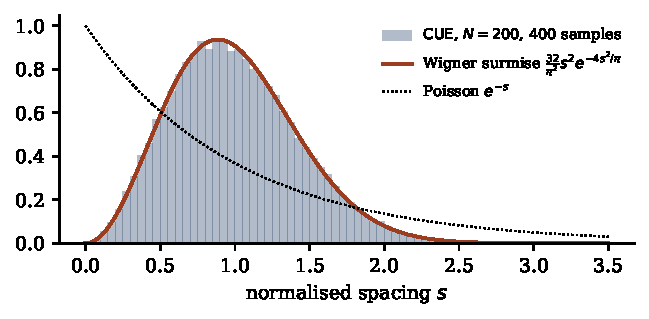
\includegraphics[width=\textwidth]{figs/ch06_spacing.pdf}
\caption{Nearest neighbour spacings of the eigenvalue angles of $400$ Haar unitary matrices of size $N=200$, scaled by $N/2\pi$ to have mean one ($80{,}000$ spacings), with the Wigner surmise $\frac{32}{\pi^2}s^2e^{-4s^2/\pi}$ for $\beta=2$ and the Poisson density $e^{-s}$. The quadratic vanishing at $s=0$ is eigenvalue repulsion.}\label{fig:ch06_spacing}
\end{figure}

\section{The Katz and Sarnak philosophy}\label{sec:ch6ks}

Katz and Sarnak \cite{katzsarnak1999,katzsarnak1999b} found that, unlike the bulk statistics, the statistics of zeros near the central point $s=\frac12$, averaged over a family, distinguish families, and that the distinction is by the symmetry type of a classical group.\index{Katz and Sarnak philosophy}

In function fields the analogous statements are theorems. Let $C$ be a smooth projective curve of genus $g$ over $\mathbb{F}_q$. Its zeta function is
\[
Z(C,u)=\frac{P_C(u)}{(1-u)(1-qu)},\qquad P_C(u)=\det\bigl(1-u\,F\mid H^1\bigr),
\]
a polynomial of degree $2g$. By Weil's theorem its roots have absolute value $q^{-1/2}$, so $P_C(q^{-1/2}u)=\det(1-u\,\vartheta_C)$ for a conjugacy class $\vartheta_C$ in $\USp(2g)$, the unitarised Frobenius; an eigenvalue $e^{i\theta}$ of $\vartheta_C$ corresponds to the zeros $s=\frac12+i(\theta+2\pi m)/\log q$, $m\in\Z$, of $Z(C,q^{-s})$. Let $C$ vary in an algebraic family, for instance the hyperelliptic curves $y^2=f(x)$ with $q$ odd and $f$ squarefree of degree $2g+1$. Deligne's equidistribution theorem \cite{deligne1980} says that as $q\to\infty$ the classes $\vartheta_C$ become equidistributed for the Haar measure of a maximal compact subgroup of the geometric monodromy group of the family, here all of $\USp(2g)$. Letting first $q\to\infty$ and then $g\to\infty$, Katz and Sarnak proved for many families over function fields that the low lying zeros follow one of a few limiting laws, labelled by the symmetry types\index{symmetry type}
\[
\mathrm{U},\quad\USp,\quad\mathrm{SO(even)},\quad\mathrm{SO(odd)},\quad\mathrm{O}.
\]

Over number fields the symmetry type of a family is conjectural: Dirichlet $L$ functions $L(s,\chi)$ with $\chi$ ranging over primitive characters of a large modulus are unitary; quadratic Dirichlet characters $\chi_d$ are symplectic; holomorphic newforms of weight $k$ and level $N$ with $N\to\infty$ are orthogonal, splitting into $\mathrm{SO(even)}$ and $\mathrm{SO(odd)}$ according to the root number; quadratic twists of a fixed elliptic curve are orthogonal, again split by root number. For several of these families the prediction has been proved, for test functions of restricted support only and assuming the generalized Riemann hypothesis where needed; Section~\ref{sec:ch6ils} treats the newforms.

To make this precise, fix an even Schwartz function $\phi$ whose Fourier transform $\hat\phi$ has compact support, so that $\phi$ extends to an entire function. For an $L$ function $L(s,f)$ in the unitary normalisation of Chapter~\ref{ch:02} (centre $\frac12$), with analytic conductor $c_f$ and nontrivial zeros $\frac12+i\gamma_f$, counted with multiplicity and not assumed to be real, the one level density\index{one level density} is $D(f;\phi)=\sum_{\gamma_f}\phi\bigl(\frac{\gamma_f}{2\pi}\log c_f\bigr)$, scaled so that the mean spacing near the central point is one. For a classical group $G(N)$ of $N\times N$ matrices, the analogous statistic $\sum_j\phi(N\theta_j/2\pi)$ of a Haar random matrix, summed over its $N$ eigenvalue angles $\theta_j\in(-\pi,\pi]$, has expectation converging to $\int\phi(x)W(G)(x)\,dx$ as $N\to\infty$, where, with $\operatorname{si}(x)=\frac{\sin2\pi x}{2\pi x}$,
\begin{align*}
W(\mathrm{U})&=1, & W(\USp)&=1-\operatorname{si},\\
W(\mathrm{SO(even)})&=1+\operatorname{si}, & W(\mathrm{SO(odd)})&=1-\operatorname{si}+\delta_0,\\
W(\mathrm{O})&=1+\tfrac12\delta_0.
\end{align*}
In Fourier terms, with $\hat W$ in the sense of distributions and $\mathbb{I}=\mathbb{I}_{[-1,1]}$ the indicator, $\hat W(\mathrm{U})=\delta_0$ and
\begin{align*}
\hat W(\USp)&=\delta_0-\tfrac12\mathbb{I}, & \hat W(\mathrm{SO(even)})&=\delta_0+\tfrac12\mathbb{I},\\
\hat W(\mathrm{O})&=\delta_0+\tfrac12, & \hat W(\mathrm{SO(odd)})&=\delta_0+1-\tfrac12\mathbb{I}.
\end{align*}
Figure~\ref{fig:ch06_onelevel} plots the densities of the first four types. The three orthogonal densities have the same Fourier transform on $(-1,1)$, so test functions with $\operatorname{supp}\hat\phi\subset(-1,1)$ cannot tell them apart; only support beyond $[-1,1]$ separates them.

\begin{figure}[t]\centering
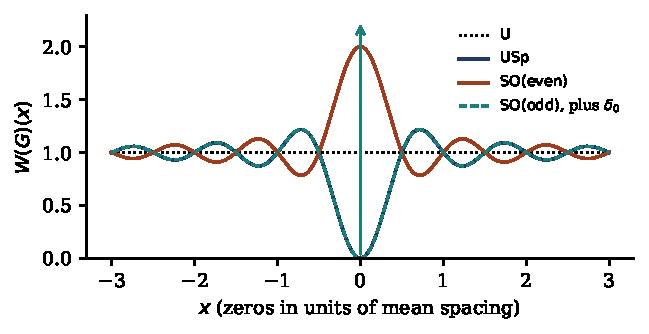
\includegraphics[width=\textwidth]{figs/ch06_onelevel.pdf}
\caption{One level densities $W(G)(x)$ of the symmetry types $\mathrm{U}$, $\USp$, $\mathrm{SO(even)}$ and $\mathrm{SO(odd)}$, with $x$ in units of the mean spacing. The symplectic density vanishes quadratically at the origin; the even orthogonal density equals $2$ there, twice the unitary value; the odd orthogonal density is the symplectic one plus a unit point mass at the origin (arrow), from the eigenvalue forced at $1$. The full orthogonal density $1+\frac12\delta_0$, not drawn, is the average of the even and odd orthogonal densities.}\label{fig:ch06_onelevel}
\end{figure}

\section{Low lying zeros of modular forms}\label{sec:ch6ils}

The first theorem over $\Q$ that separates the orthogonal types is due to Iwaniec, Luo and Sarnak \cite{ils2000}, and its method is the template for later work.\index{low lying zeros}

\begin{theorem}[Iwaniec, Luo and Sarnak \cite{ils2000}]\label{thm:ch6ils}
Assume the generalized Riemann hypothesis for the $L$ functions of holomorphic newforms and for Dirichlet $L$ functions. Fix an even weight $k$, let $N$ run through squarefree integers, and let $H_k^*(N)$ be the set of holomorphic newforms of weight $k$ and level $N$, with analytic conductor $c_f=k^2N$, and $H_k^\pm(N)$ the subsets of root number $\pm1$. Let $\phi$ be an even Schwartz function with $\operatorname{supp}\hat\phi\subset(-2,2)$. Then
\[
\lim_{N\to\infty}\frac{1}{|H_k^\pm(N)|}\sum_{f\in H_k^\pm(N)}D(f;\phi)=\int\phi(x)W(\mathrm{SO}(\pm))(x)\,dx,
\]
where $\mathrm{SO}(+)=\mathrm{SO(even)}$ and $\mathrm{SO}(-)=\mathrm{SO(odd)}$; for the full family $H_k^*(N)$ the limit is $\int\phi\,W(\mathrm{O})$. For $\operatorname{supp}\hat\phi\subset(-1,1)$ the limits for $H_k^\pm(N)$ hold as $kN\to\infty$, without the hypothesis on Dirichlet $L$ functions.
\end{theorem}

Averaging also over the weight brings in level one, where the root number is $i^k$: under the same hypotheses Iwaniec, Luo and Sarnak prove these limits for the forms of weight $k\le K$ and fixed level as $K\to\infty$, with support in $(-2,2)$. For the level one forms of weight $k\le K$, not split by root number and weighted by the harmonic weights of the Petersson formula, proportional to $L(1,\Sym^2f)^{-1}$, they prove the orthogonal limit $\int\phi\,W(\mathrm{O})$ for $\operatorname{supp}\hat\phi\subset(-2,2)$ unconditionally.

The proof starts from the explicit formula, which for $f\in H_k^*(N)$, assuming also the Riemann hypothesis for $L(s,\Sym^2f)$, gives\index{explicit formula}
\[
D(f;\phi)=\hat\phi(0)+\tfrac12\phi(0)-\frac{2}{\log c_f}\sum_{p\nmid N}\lambda_f(p)\hat\phi\Bigl(\frac{\log p}{\log c_f}\Bigr)\frac{\log p}{\sqrt p}+O\Bigl(\frac{\log\log3kN}{\log c_f}\Bigr),
\]
with $\lambda_f(p)=x_p\in[-2,2]$ the normalised Hecke eigenvalues. The term $\frac12\phi(0)$ comes from the prime squares. The coefficient of $p^{-2s}$ in $-L'/L(s,f)$ is $(\lambda_f(p)^2-2)\log p=(\lambda_f(p^2)-1)\log p$; the part with $\lambda_f(p^2)$ is negligible (this is where the Riemann hypothesis for the symmetric square enters; Iwaniec, Luo and Sarnak note that on average over the family Petersson's formula replaces it, for the same support, so the theorem does not assume it), and the constant $-1$, summed by the prime number theorem, gives $\frac12\phi(0)$. For a symplectic family such as $L(s,\chi_d)$ the coefficient is $\chi_d(p)^2\log p=\log p$ and the same sum gives $-\frac12\phi(0)$. This is the arithmetic shadow of the mean shift $\E\tr U^2=\pm1$ in orthogonal and symplectic groups. Petersson's formula then averages the sum over primes. For $\operatorname{supp}\hat\phi\subset(-1,1)$ its Kloosterman terms are negligible, so the prime sum averages to $o(1)$ and the average of $D(f;\phi)$ is $\hat\phi(0)+\frac12\phi(0)$ for both root numbers, in keeping with the agreement of the three orthogonal densities there. Beyond $(-1,1)$ these terms, evaluated with the generalized Riemann hypothesis for Dirichlet $L$ functions, contribute main terms of opposite signs to the two root numbers, through $\varepsilon_f=i^k\mu(N)\sqrt N\lambda_f(N)$; they cancel in the full family, and they are what separates $\mathrm{SO(even)}$ from $\mathrm{SO(odd)}$.

Under the generalized Riemann hypothesis the zeros are real, so if $\phi\ge0$ and $\phi(0)=1$ the order of vanishing of $L(s,f)$ at $\frac12$ is at most $D(f;\phi)$. Averaging over the family and choosing $\phi$ well, Iwaniec, Luo and Sarnak deduce that for all large squarefree $N$ more than $\frac9{16}$ of the forms in $H_k^+(N)$ have $L(\frac12,f)\ne0$ and more than $\frac{15}{16}$ of those in $H_k^-(N)$ have $L'(\frac12,f)\ne0$; the extension of the support beyond $(-1,1)$ is essential for these constants. For test functions of unrestricted support the Katz and Sarnak prediction is not known for any family over a number field.

\subsection{Why the central point sees the group}

For a self dual $L$ function the zeros are symmetric about $s=\frac12$, just as the eigenvalues of orthogonal and symplectic matrices come in pairs $e^{\pm i\theta}$; a matrix in $\mathrm{SO}(2N+1)$ always has the eigenvalue $1$, as an $L$ function of root number $-1$ vanishes at $\frac12$. Away from the symmetry point all groups look unitary; near it, the factor $\prod\sin^2\theta_j$ or $\prod\sin^2(\theta_j/2)$ in the Weyl density decides whether eigenvalues are repelled from $1$. Low lying zeros thus measure the Weyl density, near the identity, of the symmetry group attached to the family.

\subsection{Ranks of elliptic curves}

If the two root numbers occur equally often and, as the Katz and Sarnak model predicts, the analytic rank is $0$ or $1$ according to the root number outside a set of density zero (the minimalist conjecture of Section~\ref{sec:06cranks}),\index{minimalist conjecture} then the average analytic rank should be $\frac12$, provided that exceptional set contributes nothing to the average. Brumer \cite{brumer1992}, Heath Brown \cite{heathbrown2004} and Young \cite{young2006} used one level density with restricted support to prove, under the generalized Riemann hypothesis, upper bounds for the average analytic rank of all elliptic curves ordered by height, with Young obtaining $\frac{25}{14}$. These are conditional theorems; the value $\frac12$ is a conjecture. Unconditional bounds for the average algebraic rank come from Selmer groups (Theorem~\ref{thm:06cbs}).

In computable ranges, families show an excess of rank two curves; Bektemirov, Mazur, Stein and Watkins \cite{bmsw2007} examine this tension between data and conjecture and argue that slow convergence can reconcile the two. Miller \cite{miller2004,miller2006} found that for small conductors the first zero above the central point is repelled more strongly than the limiting density predicts. Due\~nez, Huynh, Keating, Miller and Snaith \cite{dhkms2012} reproduce this repulsion with an excised orthogonal ensemble, which discards the matrices in $\mathrm{SO}(2N)$ whose characteristic polynomial at $1$ is too small, mimicking the discreteness of central values imposed by the formulas of Waldspurger and of Kohnen and Zagier; this is a model, not a theorem.

\section{Moments and the Keating and Snaith conjectures}\label{sec:ch6ksnaith}

Random matrices also predict the size of $L$ functions at the central point. Let $Z_N(\theta)=\det(I-U_Ne^{-i\theta})$ be the characteristic polynomial of a Haar unitary matrix. Keating and Snaith \cite{keatingsnaith2000} computed, using Selberg's integral,
\[
\E|Z_N(0)|^{2k}=\prod_{j=1}^N\frac{\Gamma(j)\Gamma(j+2k)}{\Gamma(j+k)^2}\sim\frac{G(k+1)^2}{G(2k+1)}N^{k^2}\qquad(N\to\infty),
\]
for $\Re k>-\frac12$, where $G$ is the Barnes $G$ function, $G(n+1)=\prod_{j=0}^{n-1}j!$ for integers $n\ge0$.\index{Keating and Snaith conjecture}\index{Barnes G function} Equating the mean density of zeros, $N\leftrightarrow\log\frac{T}{2\pi}$, and inserting an arithmetic factor that random matrices cannot see, they proposed the following.

\begin{conjecture}[Keating and Snaith]\label{conj:ch6ks}
For each $k>-\frac12$, as $T\to\infty$,
\[
\frac1T\int_0^T\bigl|\zeta(\tfrac12+it)\bigr|^{2k}dt\sim a_k\,\frac{G(k+1)^2}{G(2k+1)}\,(\log T)^{k^2},
\]
with $a_k=\prod_p(1-p^{-1})^{k^2}\sum_{m\ge0}\Bigl(\frac{\Gamma(m+k)}{m!\,\Gamma(k)}\Bigr)^2p^{-m}$.
\end{conjecture}

For $k=1$ the right side is $\log T$ (Hardy and Littlewood), and for $k=2$ it is $\frac{1}{2\pi^2}(\log T)^4$ (Ingham), since $G(3)^2/G(5)=\frac1{12}$ and $a_2=6/\pi^2$. For $k=3$ and $k=4$ the leading coefficients are $42a_3/9!$ and $24024a_4/16!$, in agreement with the conjectures of Conrey and Ghosh \cite{conreyghosh1998} and of Conrey and Gonek \cite{conreygonek2001}. No case other than $k=0,1,2$ is proved. Lower order terms are predicted by the recipe of Conrey, Farmer, Keating, Rubinstein and Snaith \cite{cfkrs2005}.

For families with symplectic or orthogonal symmetry, Keating and Snaith \cite{keatingsnaith2000b} computed the moments of $\det(I-U)$ for Haar $U$ in $\USp(2N)$ and in $\mathrm{SO}(2N)$; for instance, for each positive integer $k$, as $N\to\infty$,
\[
\E_{\USp(2N)}\det(I-U)^k\sim g_kN^{k(k+1)/2},\qquad g_k=2^{k(k+1)/2}\prod_{j=1}^k\frac{j!}{(2j)!}.
\]
A matrix in $\USp(2N)$ has $2N$ eigenvalues, so equating densities of zeros matches $2N$, not $N$, with the logarithm of the conductor, and they conjectured, for example, that
\[
\frac{1}{X^*}\sum_{0<d\le X}^{\flat}L(\tfrac12,\chi_d)^k\sim b_k\,g_k\Bigl(\frac{\log X}{2}\Bigr)^{k(k+1)/2},
\]
where the sum runs over the $X^*\sim3X/\pi^2$ fundamental discriminants $0<d\le X$ and $b_k$ is an explicit Euler product, the analogue of $a_k$. The exponent $k(k+1)/2$ identifies the family as symplectic; for orthogonal families it is $k(k-1)/2$. Jutila \cite{jutila1981} proved the cases $k=1,2$, and Soundararajan \cite{soundararajan2000} the case $k=3$ for the closely related family of characters $\chi_{8d}$; Shen \cite{shen2021} proved the case $k=4$ for that family under the generalized Riemann hypothesis, and Shen and Stucky \cite{shenstucky2024} remove the hypothesis in a preprint. The ratios conjecture of Conrey, Farmer and Zirnbauer \cite{cfz2008}, applied by Conrey and Snaith \cite{conreysnaith2007}, predicts the one level density with all lower order terms, for test functions of arbitrary support.\index{ratios conjecture}

\section{Two random matrix limits}\label{sec:ch6two}

The Sato Tate limit of Chapters~\ref{ch:03} and \ref{ch:04} fixes $\pi$ and varies $p$: the Satake parameters $A_p(\pi)$ are conjectured to become equidistributed for the Haar measure of a fixed compact group $\mathrm{ST}(\pi)$ (Conjecture~\ref{conj:ch3gst} for abelian varieties). This is a theorem for elliptic curves over $\Q$ without complex multiplication, where the group is $\SU(2)$ (Theorem~\ref{thm:04STthm}), and open for a generic abelian surface, where it is $\USp(4)$. Its vertical versions fix $p$ and vary the object.\index{vertical Sato Tate theorem} For the eigenvalues of $T_p$ on spaces of modular forms of growing level or weight, the limit is the Kesten McKay law $\mu_p$ (Serre \cite{serre1997}; Conrey, Duke and Farmer \cite{cdf1997}; Theorem~\ref{thm:07serre}), which depends on $p$ and tends to the Sato Tate law as $p\to\infty$. For all elliptic curves $y^2=x^3+ax+b$ over $\mathbb{F}_p$, Birch \cite{birch1968} computed the moments of the traces of Frobenius and showed that their normalised values become semicircle distributed as $p\to\infty$; Deligne's equidistribution theorem of Section~\ref{sec:ch6ks} recovers this as a case of genus one.

The Katz and Sarnak limit of this chapter models the zeros of $L(s,f)$ near the central point by the eigenvalues of a random matrix whose size grows like $\log c_f$, so the groups have dimension tending to infinity. For curves over $\mathbb{F}_q$ both limits concern the same classes $\vartheta_C\in\USp(2g)$: at fixed $g$, Deligne's theorem as $q\to\infty$ is a vertical Sato Tate law for $\vartheta_C$, whose trace is $-(\#C(\mathbb{F}_q)-q-1)/\sqrt q$, and Katz and Sarnak then let $g\to\infty$ and study the eigenvalues near $1$. Over number fields the link between the two limits is the explicit formula, which expresses sums over zeros through the Satake parameters $A_p(\pi)$.

\section{Notes}

Montgomery's paper \cite{montgomery1973} states the pair correlation conjecture explicitly, and Odlyzko's computations \cite{odlyzko1987} remain the principal numerical evidence for the unitary model. For eigenvalue statistics of compact classical groups, Mehta's book \cite{mehta2004}, the monograph of Katz and Sarnak \cite{katzsarnak1999} and Meckes's book \cite{meckes2019} are standard, and the survey of Katz and Sarnak \cite{katzsarnak1999b} is the shortest route to the symmetry types. Beyond Theorem~\ref{thm:ch6ds}, suitably normalised powers $|Z_N|^{2\alpha}$ converge to Gaussian multiplicative chaos for $\alpha$ below a critical value (Webb \cite{webb2015}; Nikula, Saksman and Webb \cite{nsw2020}), and the maximum of $\log|Z_N|$ on the circle is known to order one (Chhaibi, Madaule and Najnudel \cite{cmn2018}), as conjectured by Fyodorov, Hiary and Keating \cite{fhk2012}; Chapter~\ref{ch:09b} takes up these log correlated questions.

\section{Exercises}

\begin{enumerate}
\item Using Proposition~\ref{prop:ch6su2}, show that $\tr A^2=x^2-2=2\cos2\theta$ for Haar $A\in\SU(2)$, that $\E\tr A^2=-1$, and that $\E\tr A^j=0$ for every other $j\ge1$. Compare with the symplectic mean shift for $\USp(2N)$ stated after Theorem~\ref{thm:ch6ds}.
\item Let $U$ be Haar in $\mathrm{U}(N)$. Show directly from the invariance $U\mapsto e^{i\alpha}U$ that $\E(\tr U^j)=0$ for $j\ge1$. Using the Weyl density for $\mathrm{U}(N)$, show that $\E|\tr U|^2=1$ for $N\ge1$ and more generally $\E|\tr U^j|^2=\min(j,N)$. Hint: the density is $\frac1{N!}\det[K_N(\theta_j,\theta_l)]_{j,l\le N}$, where
\[
K_N(\theta,\theta')=\frac1{2\pi}\sum_{m=0}^{N-1}e^{im(\theta-\theta')}.
\]
\item Let $\theta_1,\dots,\theta_g$ have the density \eqref{eq:ch6usp} and put $t=\sum_j2\cos\theta_j$, the trace of a Haar element of $\USp(2g)$. Show that $\E t^2=1$ for every $g$, using that $t$ is the character of an irreducible representation. Deduce from Deligne's equidistribution theorem, as stated in Section~\ref{sec:ch6ks}, that for the hyperelliptic curves of genus $g$ over $\mathbb{F}_q$ the mean of $\#C(\mathbb{F}_q)$ is $q+1+o(\sqrt q)$ and its variance is $(1+o(1))q$ as $q\to\infty$.
\item Compute the Fourier transforms of $1\pm\frac{\sin2\pi x}{2\pi x}$ and verify the formulas for $\hat W$; note that the point mass $\delta_0$ in $W(\mathrm{SO(odd)})$ becomes the constant $1$ in $\hat W(\mathrm{SO(odd)})$. Deduce that if $\operatorname{supp}\hat\phi\subset(-1,1)$ then $\int\phi\,W(G)=\hat\phi(0)+\frac12\phi(0)$ for all three orthogonal types and $\hat\phi(0)-\frac12\phi(0)$ for $\USp$, and compare with the explicit formula of Section~\ref{sec:ch6ils}. Check that $W(\mathrm{O})$ is the average of $W(\mathrm{SO(even)})$ and $W(\mathrm{SO(odd)})$.
\item Verify the identities
\[
\frac{G(3)^2}{G(5)}=\frac1{12},\qquad\frac{G(4)^2}{G(7)}=\frac{42}{9!},\qquad\frac{G(5)^2}{G(9)}=\frac{24024}{16!}.
\]
Show that $\log\bigl(G(k+1)^2/G(2k+1)\bigr)\sim-k^2\log k$ as $k\to\infty$. Since $\log|Z_N(0)|$ is approximately Gaussian with variance $\frac12\log N$, a Gaussian model predicts $\E|Z_N(0)|^{2k}\approx N^{k^2}$ with no constant depending on $k$; interpret the decay of $G(k+1)^2/G(2k+1)$ in terms of the upper tail of $\log|Z_N(0)|$ at the scale $k\log N$.
\end{enumerate}

\section{Open computational problems}

\begin{compproblem}[One level density for quadratic twists of 11a]
Objective: measure the one level density of the family of quadratic twists of the curve $11a$, separated by root number, and compare it with $W(\mathrm{SO(even)})$ and $W(\mathrm{SO(odd)})$ including lower order terms. Objects: all twists $E_d$ of $y^2+y=x^3-x^2-10x-20$ by fundamental discriminants $d$ coprime to $11$ with conductor $11d^2\le10^8$, so that $|d|$ runs up to about $3000$ and the root number of $E_d$ is $\chi_d(-11)$; the lowest ten zeros of each $L(s,E_d)$. Route: PARI/GP \texttt{lfunzeros} or Rubinstein's \texttt{lcalc}, with $a_p(E_d)=\chi_d(p)a_p(E)$ computed once; parallel over $d$. Deliverable: histograms of scaled zeros near the central point for each sign, the empirical one level density for several test functions with Fourier support up to $2$ and beyond, the distribution of the first zero, and a fit to the ratios conjecture prediction with finite conductor corrections. Why it matters: it tests the Katz and Sarnak prediction in a family where theorems of the type of Theorem~\ref{thm:ch6ils} cover only restricted support, quantifies the repulsion of the first zero observed by Miller and modelled by the excised orthogonal ensemble, and connects with the excess rank question.
\end{compproblem}

\begin{compproblem}[Keating and Snaith versus numerical moments of quadratic \texorpdfstring{$L$}{L} functions]
Objective: compare the conjectured asymptotics for $\sum_{|d|\le X}L(\frac12,\chi_d)^k$ with numerical data, for $k=1,\dots,6$, and estimate the lower order terms. Objects: all fundamental discriminants $|d|\le10^9$, or a random subset of comparable size at larger $X$. Route: compute $L(\frac12,\chi_d)$ by the approximate functional equation with smoothed sums, on GPUs, or with PARI/GP \texttt{lfun} for smaller ranges; evaluate the full CFKRS polynomial in $\log X$ for each $k$ and the ratios conjecture predictions. Deliverable: tables of empirical moments against the leading term and against the full polynomial, plots of the relative error against $X$, and an empirical estimate of the power savings in the error term. Why it matters: the symplectic exponent $k(k+1)/2$ is the random matrix signature of the family; the numerical residuals measure how accurately the CFKRS recipe captures arithmetic beyond the leading constant, and for $k\ge5$ no asymptotic is known, even conditionally.
\end{compproblem}

\begin{compproblem}[Nearest neighbour spacings for the zeros of \texorpdfstring{$L(s,\Delta)$}{L(s,Delta)} at large height]
Objective: test unitary statistics for the zeros of the $L$ function of the Ramanujan $\Delta$ function, a degree two $L$ function, at heights comparable to those of Odlyzko's zeta computations, continuing Problem~\ref{cp:09bpair}, whose highest block of zeros lies near height $10^7$. Objects: blocks of $10^6$ to $10^7$ consecutive zeros of $L(s,\Delta)$ near height $10^{8}$, where the zero density is about $5$ per unit height, and blocks of up to $10^9$ zeros near $10^{10}$ and, as a long term target, near $10^{20}$. Route: at moderate heights use the approximate functional equation in \texttt{lcalc} or ARB; at large heights an analogue of the Odlyzko and Schönhage algorithm for degree two (multipoint evaluation of $\sum\tau(n)n^{-11/2-s}$ with fast summation, or Hiary's methods adapted to modular forms) must be developed, and the feasibility at $10^{20}$ is itself part of the problem. Deliverable: empirical spacing distributions against the Gaudin law, pair correlation, number variance, and the arithmetic lower order corrections predicted by Bogomolny and Keating type formulas. Why it matters: Rudnick and Sarnak prove GUE correlations for $L(s,\Delta)$ only for restricted test functions, and between heights $500$ and $2000$ the spacings of its zeros are markedly more rigid than the Gaudin law (variance $0.138$ against $0.180$, Chapter~\ref{ch:09b}); large height data would show how fast a degree two $L$ function approaches the unitary limit, where the arithmetic corrections involve $\Sym^2\Delta$.
\end{compproblem}

\chapter{Kloosterman Sums: Vertical Sato Tate and Random Fourier Series}\label{ch:06b}

In 1926 Kloosterman, counting representations of integers by quaternary quadratic forms with the circle method, met the exponential sums that now bear his name and proved that they are smaller than trivial by a power of the modulus \cite{kloosterman1926}. Twenty two years later Weil deduced the optimal bound from the Riemann hypothesis for curves over finite fields \cite{weil1948b}, and forty years after that Katz determined the statistical law of the normalised sums: as the prime grows, Kloosterman angles are distributed like the angles of Haar random matrices in $\SU(2)$ \cite{katz1988}. The same semicircle that governs Frobenius traces of elliptic curves (Chapter~\ref{ch:04}) and the eigenvalues of random matrices (Chapter~\ref{ch:06}) thus governs a family of exponential sums with no elliptic curve in sight. Kloosterman sums are also tied to the spectral theory of automorphic forms: the Bruggeman Kuznetsov formula equates sums of them with spectral averages of Fourier coefficients of Maass forms, and Selberg's bound $\lambda_1\ge 3/16$ is Weil's bound read spectrally. In the last part of the chapter we follow Kowalski and Sawin \cite{kowalskisawin2016}, who joined partial Kloosterman sums into polygonal paths and found in the limit a random Fourier series with independent Sato Tate coefficients. We prove the analytic reduction behind their theorem, compute the covariance of the limit in closed form, and show exactly how a change of parametrisation removes one Sato Tate coefficient from the limit, the effect behind a variance deficit of $1/\pi^2$ that our computations ran into.

\section{Kloosterman sums and Weil's bound}\label{sec:06bweil}

Let $p$ be an odd prime and write $e(z)=e^{2\pi iz}$. For $x\in\mathbb{F}_p^\times$ let $\bar x$ denote its inverse. For $a,b\in\mathbb{F}_p$ the \emph{Kloosterman sum}\index{Kloosterman sum} is
\[
\mathrm{Kl}(a,b;p)=\sum_{x\in\mathbb{F}_p^\times}e\Bigl(\frac{ax+b\bar x}{p}\Bigr),
\]
and we abbreviate $\mathrm{Kl}(c;p)=\mathrm{Kl}(c,1;p)$. Three elementary properties are used constantly (Exercise~\ref{ex:06bbasic}). First, $\mathrm{Kl}(a,b;p)$ is real, because $x\mapsto -x$ maps the sum to its complex conjugate. Second, if $a\ne0$ the substitution $y=ax$ gives $\mathrm{Kl}(a,b;p)=\mathrm{Kl}(1,ab;p)$, so the sum depends only on the product $ab$ when $a\neq 0$; by symmetry the same holds when $b\ne0$, so $\mathrm{Kl}(a,b;p)=\mathrm{Kl}(ab;p)$ unless $a=b=0$. Third, if exactly one of $a,b$ vanishes the sum is a Ramanujan sum: $\sum_{x\neq0}e(cx/p)=-1$ for $c\ne0$, so $\mathrm{Kl}(0;p)=-1$.

The trivial bound is $|\mathrm{Kl}(a;p)|\le p-1$. The moments show that the typical size is $\sqrt p$.

\begin{proposition}[Second and fourth moments]\label{prop:06bmoments}
For every odd prime $p$,
\begin{gather*}
\sum_{a\in\mathbb{F}_p^\times}\mathrm{Kl}(a;p)=1,\qquad
\sum_{a\in\mathbb{F}_p^\times}\mathrm{Kl}(a;p)^2=p^2-p-1,\\
\sum_{a\in\mathbb{F}_p^\times}\mathrm{Kl}(a;p)^4=2p^3-3p^2-3p-1 .
\end{gather*}
Consequently the normalised values $x_{p,a}=\mathrm{Kl}(a;p)/\sqrt p$ have empirical second moment $1-1/(p(p-1))$ and empirical fourth moment $2-1/p+O(p^{-2})$ over $a\in\mathbb{F}_p^\times$.
\end{proposition}

These identities are classical; we include the proof because the fourth moment is the first place where the semicircle appears.

\begin{proof}
We sum over all $a\in\mathbb{F}_p$ and subtract the term $a=0$, where $\mathrm{Kl}(0;p)=-1$. By orthogonality of additive characters, $\sum_ae(au/p)=p\,\mathbb{I}_{u=0}$, we have $\sum_a\mathrm{Kl}(a;p)=\sum_{x\ne0}e(\bar x/p)\sum_ae(ax/p)=0$, and, since $\mathrm{Kl}(a;p)$ is real,
\[
\sum_a\mathrm{Kl}(a;p)^2=\sum_{x,y\ne0}e\Bigl(\frac{\bar x-\bar y}{p}\Bigr)\sum_ae\Bigl(\frac{a(x-y)}{p}\Bigr)=p(p-1).
\]
For the fourth moment write $\mathrm{Kl}(a;p)^2=\sum_{u}e(au/p)T(u)$ with
\[
T(u)=\sum_{\substack{x,y\ne0\\ x+y=u}}e\Bigl(\frac{\bar x+\bar y}{p}\Bigr).
\]
Since $\mathrm{Kl}^2$ is real, Parseval gives $\sum_a\mathrm{Kl}(a;p)^4=\sum_a|\mathrm{Kl}(a;p)^2|^2=p\sum_u|T(u)|^2$. For $u=0$ we have $y=-x$, hence $\bar y=-\bar x$, and $T(0)=p-1$. For $u\ne0$ we have $\bar x+\bar y=u\,\overline{x(u-x)}$, and the substitution $x=us$ gives $T(u)=\sum_{s\ne0,1}e(\bar u\,\overline{s(1-s)}/p)$. The equation $s(1-s)=v$ has $1+\bigl(\frac{1-4v}{p}\bigr)$ solutions, with $\bigl(\frac{\cdot}{p}\bigr)$ the Legendre symbol $\chi$. Writing $w=\bar v$ and using $\chi(1-4\bar w)=\chi(w(w-4))$,
\[
T(u)=-1+G(\bar u),\qquad G(c)=\sum_{w\in\mathbb{F}_p}\chi\bigl(w(w-4)\bigr)e(cw/p).
\]
Now $G(0)=\sum_w\chi(w^2-4w)=-1$ (a quadratic with nonzero discriminant), $\sum_cG(c)=p\,\chi(0)=0$, and by Parseval $\sum_c|G(c)|^2=p\,\#\{w:w(w-4)\ne0\}=p(p-2)$. Hence $\sum_{c\ne0}|G(c)|^2=p^2-2p-1$ and $\sum_{c\ne0}G(c)=1$, so
\[
\sum_{u\ne0}|T(u)|^2=\sum_{c\ne0}|G(c)-1|^2=(p^2-2p-1)-2+(p-1)=p^2-p-4 .
\]
With $T(0)^2=(p-1)^2$ added, $\sum_u|T(u)|^2=2p^2-3p-3$, so $\sum_{a\in\mathbb{F}_p}\mathrm{Kl}(a;p)^4=2p^3-3p^2-3p$, and removing $a=0$ proves the claim.
\end{proof}

The limits $1$ and $2$ are the first two even moments of the Sato Tate law $\ST$, the Catalan numbers $C_1,C_2$ of Chapter~\ref{ch:04}. The second moment shows that $\max_a|\mathrm{Kl}(a;p)|\ge\sqrt{p}\,(1+o(1))$. The fourth moment gives $\max_a|\mathrm{Kl}(a;p)|^4\le2p^3$, that is $|\mathrm{Kl}(a;p)|\le2^{1/4}p^{3/4}$, which is essentially Kloosterman's bound. A bound of the right order $p^{k+1}$ for the moment of order $2k$ would give the exponent $\frac12+\frac1{2k}$, but proving it already requires the geometry behind the optimal bound.

\begin{theorem}[Weil \cite{weil1948b}]\label{thm:06bweil}\index{Weil bound}
For $p\nmid ab$, $|\mathrm{Kl}(a,b;p)|\le 2\sqrt p$.
\end{theorem}

\paragraph{Idea of proof.} By the second property above we may take $b=1$ and $a\ne0$. For $n\ge1$ let $\mathrm{Kl}_n(a)=\sum_{x\in\mathbb{F}_{p^n}^\times}\psi\bigl(\mathrm{Tr}_{\mathbb{F}_{p^n}/\mathbb{F}_p}(ax+\bar x)\bigr)$ with $\psi(z)=e(z/p)$, so that $\mathrm{Kl}_1(a)=\mathrm{Kl}(a;p)$. To a monic $f\in\mathbb{F}_p[X]$ with $f(0)\ne0$ attach $\lambda(f)=\psi\bigl(a\sigma(f)+\sigma'(f)\bigr)$, where $\sigma(f)$ and $\sigma'(f)$ are the sums of the roots of $f$ and of their inverses. Then $\lambda$ is completely multiplicative, and grouping the $x\in\mathbb{F}_{p^n}^\times$ by their minimal polynomials over $\mathbb{F}_p$ turns the Euler product over irreducible $f$ into
\[
L_a(T)=\exp\Bigl(\sum_{n\ge1}\mathrm{Kl}_n(a)\frac{T^n}{n}\Bigr)=\sum_{f}\lambda(f)\,T^{\deg f}.
\]
For $f=X^d+c_{d-1}X^{d-1}+\dots+c_0$ we have $\sigma(f)=-c_{d-1}$ and $\sigma'(f)=-c_1/c_0$. When $d\ge3$ the coefficient $c_{d-1}$ is free and the terms of degree $d$ cancel because $a\ne0$; counting the terms of degrees $1$ and $2$ gives $L_a(T)=1+\mathrm{Kl}(a;p)\,T+pT^2$. This is Weil's argument \cite{weil1948b}. Factor $L_a(T)=(1-\alpha T)(1-\beta T)$; then $\mathrm{Kl}_n(a)=-(\alpha^n+\beta^n)$ and $\alpha\beta=p$. Counting the points of the Artin Schreier curve $y^p-y=ax+1/x$, which has genus $p-1$, over $\mathbb{F}_{p^n}$ shows that $\alpha$ and $\beta$ are among the reciprocal roots of the numerator of its zeta function, so the Riemann hypothesis for curves gives $|\alpha|=|\beta|=\sqrt p$, hence the bound. Conversely, a bound $|\mathrm{Kl}_n(a)|\le Cp^{n/2}$ with $C$ independent of $n$ already forces $|\alpha|=|\beta|=\sqrt p$ (Exercise~\ref{ex:06bweilL}). The elementary method of Stepanov \cite{stepanov1969}, in Bombieri's form \cite{bombieri1974}, proves point count bounds of exactly this kind over every extension $\mathbb{F}_{p^n}$, and so reaches the same conclusion.

Since $\alpha\beta=p$, $|\alpha|=|\beta|=\sqrt p$ and $\alpha+\beta=-\mathrm{Kl}(a;p)$ is real, we have $\beta=\bar\alpha$, and we may write $\{\alpha,\beta\}=\{-\sqrt p\,e^{i\theta},-\sqrt p\,e^{-i\theta}\}$ with a unique \emph{Kloosterman angle} $\theta_{p,a}\in[0,\pi]$, so that
\[
x_{p,a}=\frac{\mathrm{Kl}(a;p)}{\sqrt p}=2\cos\theta_{p,a}\in[-2,2].
\]
In the language of $\ell$ adic sheaves, Deligne and Katz construct a rank two lisse sheaf $\mathcal{K}l$ on $\mathbb{G}_m$ over $\mathbb{F}_p$, pure of weight one, whose Frobenius at $a\in\mathbb{F}_p^\times$ has eigenvalues $\alpha,\beta$ and trace $-\mathrm{Kl}(a;p)$ \cite{katz1988}. After the half Tate twist the Frobenius at $a$ determines a conjugacy class in $\SU(2)$, exactly like the Satake parameter $\mathrm{diag}(e^{i\theta_p},e^{-i\theta_p})$ of a modular form at a prime $p$. Kloosterman angles and Satake angles live on the same circle; the sign in the trace is immaterial for us because $\ST$ is invariant under $\theta\mapsto\pi-\theta$.

\section{Katz's theorem: vertical Sato Tate}\label{sec:06bkatz}

There are two ways to let the Kloosterman angles vary. \emph{Vertically}, fix $p$ and let $a$ run over $\mathbb{F}_p^\times$, then let $p\to\infty$. \emph{Horizontally}, fix $a$ and let $p$ run over the primes. The vertical problem is the analogue of the vertical Sato Tate theorem for Hecke eigenvalues in Chapter~\ref{ch:07}; the horizontal problem is the analogue of Sato Tate for a fixed elliptic curve.

\begin{theorem}[Katz \cite{katz1988}]\label{thm:06bkatz}\index{Katz equidistribution theorem}\index{vertical Sato Tate theorem}
As $p\to\infty$ the multisets $\{\theta_{p,a}:a\in\mathbb{F}_p^\times\}$ become equidistributed in $[0,\pi]$ with respect to the Sato Tate measure $\frac2\pi\sin^2\theta\,d\theta$. Equivalently, for every continuous $f$ on $[-2,2]$,
\[
\frac{1}{p-1}\sum_{a\in\mathbb{F}_p^\times}f\Bigl(\frac{\mathrm{Kl}(a;p)}{\sqrt p}\Bigr)\longrightarrow\int_{-2}^2f\,d\ST .
\]
\end{theorem}

Since $\mathrm{Kl}(a,b;p)=\mathrm{Kl}(ab;p)$ and $a\mapsto ab$ permutes $\mathbb{F}_p^\times$ when $p\nmid b$, the same holds for $\mathrm{Kl}(a,b;p)$ with $b$ fixed.

\paragraph{Proof sketch.} By the Weyl criterion (Theorem~\ref{thm:04weyl}, whose proof applies verbatim to any sequence of probability measures on $[0,\pi]$) it suffices to show that the averages of $U_n(\cos\theta_{p,a})$ tend to zero for each $n\ge1$. Up to the sign $(-1)^n$, $U_n(\cos\theta_{p,a})$ is the trace of Frobenius at $a$ on $\Sym^n$ of the normalised sheaf. By the Grothendieck Lefschetz trace formula,
\[
\sum_{a\in\mathbb{F}_p^\times}\tr\bigl(\Frob_a\mid\Sym^n\mathcal{K}l\bigr)=\sum_{i=0}^2(-1)^i\tr\bigl(\Frob\mid H^i_c(\mathbb{G}_{m,\bar{\mathbb{F}}_p},\Sym^n\mathcal{K}l)\bigr).
\]
The group $H^0_c$ vanishes because $\mathbb{G}_m$ is affine. The group $H^2_c$ is the space of coinvariants of the geometric monodromy group acting on $\Sym^n$, and Katz proved that this group is $\SL_2$ \cite{katz1988}. The inputs are local: the sheaf has geometrically trivial determinant, it is tamely ramified at $0$ with unipotent local monodromy consisting of a single Jordan block, and it is wildly ramified at $\infty$ with both breaks equal to $\frac12$ (Swan conductor $1$); Katz deduces from them that no proper subgroup of $\SL_2$ can be the geometric monodromy group. Since $\Sym^n$ is an irreducible nontrivial representation of $\SL_2$ for $n\ge1$, the coinvariants vanish. Finally, by Deligne's Weil II \cite{deligne1980} the eigenvalues of Frobenius on $H^1_c$ have absolute value at most $\sqrt p$ after normalisation, and the Grothendieck Ogg Shafarevich formula gives $\dim H^1_c=\mathrm{Swan}_\infty(\Sym^n\mathcal{K}l)\le\frac{n+1}2$, because $\Sym^n\mathcal{K}l$ is tame at $0$ and its breaks at $\infty$ are at most $\frac12$. Therefore
\[
\Bigl|\frac{1}{p-1}\sum_{a\in\mathbb{F}_p^\times}U_n(\cos\theta_{p,a})\Bigr|\le\frac{(n+1)\sqrt p}{2(p-1)}\le\frac{n+1}{\sqrt p}.
\]

This is Deligne's equidistribution theorem \cite{deligne1980} applied to the Kloosterman sheaf, and the monodromy computation is the heart of the matter; Katz and Sarnak use exactly this mechanism to produce the random matrix statistics of Chapter~\ref{ch:06} \cite{katzsarnak1999}. The bound $(n+1)/\sqrt p$ for the Weyl sums gives an explicit rate in the discrepancy, worked out by Niederreiter \cite{niederreiter1991}. Katz also computed the monodromy of the hyper Kloosterman sheaves of rank $n$: it is the symplectic group $\mathrm{Sp}_n$ for even $n$, and $\SL_n$ for odd $n$ when $p$ is odd \cite{katz1988}. The case $n=2$ of this chapter is the first member of the symplectic series, since $\SL_2=\mathrm{Sp}_2$ and $\SU(2)=\USp(2)$.

For the paths of Section~\ref{sec:06bpaths} we need a joint statement for additive shifts.

\begin{theorem}[Joint equidistribution of shifts]\label{thm:06bjoint}
Let $h_1,\dots,h_k$ be distinct integers. As $p\to\infty$, with $a$ uniform among the elements of $\mathbb{F}_p$ for which $a+h_j\ne0$ for all $j$, the random vector $\bigl(\mathrm{Kl}(a+h_1;p),\dots,\mathrm{Kl}(a+h_k;p)\bigr)/\sqrt p$ converges in law to $(\mathrm{ST}_1,\dots,\mathrm{ST}_k)$, independent random variables with law $\ST$.
\end{theorem}

This is due to Kowalski and Sawin \cite{kowalskisawin2016}, who deduce it from Katz's computation of the monodromy. The relevant monodromy group is now that of the direct sum of the translated sheaves $[x\mapsto x+h_j]^*\mathcal{K}l$, a subgroup of $\SL_2^k$ projecting onto each factor. By the Goursat Kolchin Ribet criterion \cite{katz1990}\index{Goursat Kolchin Ribet criterion} it is all of $\SL_2^k$ unless two of the translates become geometrically isomorphic after tensoring with a rank one sheaf. The ramification at $0$ rules this out. Pulling back by $x\mapsto x-h_i$, we may compare $\mathcal{K}l$ itself with its translate $[x\mapsto x+h]^*\mathcal{K}l$, where $h=h_j-h_i\neq0$, and an isomorphism $[x\mapsto x+h]^*\mathcal{K}l\simeq\mathcal{K}l\otimes\mathcal{L}$ is impossible: the translate is lisse at $0$, while $\mathcal{K}l\otimes\mathcal{L}$ is ramified at $0$ for every rank one sheaf $\mathcal{L}$, because the local monodromy of $\mathcal{K}l$ at $0$ is a nontrivial unipotent block. Joint equidistribution then follows from Deligne's theorem with $\SU(2)^k$ in place of $\SU(2)$: the Kloosterman sums at distinct additive shifts behave like independent traces of Haar random matrices.

\subsection{Data}

For this book we computed $\mathrm{Kl}(a;p)=\sum_{x=1}^{p-1}e((x+a\bar x)/p)$ for all $a$ at $p=1009$ and $p=10007$, and for $3000$ random $a$ at $p=100003$. Table~\ref{tab:06bkatz} compares the even moments of $\mathrm{Kl}/\sqrt p$ with the Catalan numbers. The second and fourth moments at $p=1009$ and $p=10007$ agree with the exact values of Proposition~\ref{prop:06bmoments} to all printed digits: for $p=1009$ the identity predicts $1-1/(1009\cdot1008)=0.999999$ and $(2p^3-3p^2-3p-1)/((p-1)p^2)=1.999005$. The largest values of $|\mathrm{Kl}|/\sqrt p$ are $1.98077$ and $1.99876$, inside Weil's interval and close to its edge, and Kolmogorov Smirnov tests against $\ST$ give $p$ values $0.918$ and $0.993$ (descriptive only, since the values $\mathrm{Kl}(a;p)$ are not independent samples). Figure~\ref{fig:06bkatz} shows the histogram at $p=10007$.

\begin{table}[t]\centering\small
\begin{tabular}{lcccc}
\toprule
& $m=1$ & $m=2$ & $m=3$ & $m=4$\\
\midrule
$p=1009$, all $a$ & $0.999999$ & $1.99900$ & $4.98271$ & $13.90784$\\
$p=10007$, all $a$ & $1.0000000$ & $1.99990$ & $5.00198$ & $14.03501$\\
$p=100003$, $3000$ values & $0.9918$ & $1.9794$ & $4.9547$ & $13.9179$\\
Catalan $C_m$ & $1$ & $2$ & $5$ & $14$\\
\bottomrule
\end{tabular}
\caption{Empirical moments $\E(\mathrm{Kl}(a;p)/\sqrt p)^{2m}$, with $a$ uniform over the values listed, against the Sato Tate moments $C_m$. For the random sample at $p=100003$ the standard errors under $\ST$, $\bigl((C_{2m}-C_m^2)/3000\bigr)^{1/2}$, are about $0.02$, $0.06$, $0.19$ and $0.64$ in the four columns.}\label{tab:06bkatz}
\end{table}

\begin{figure}[t]\centering
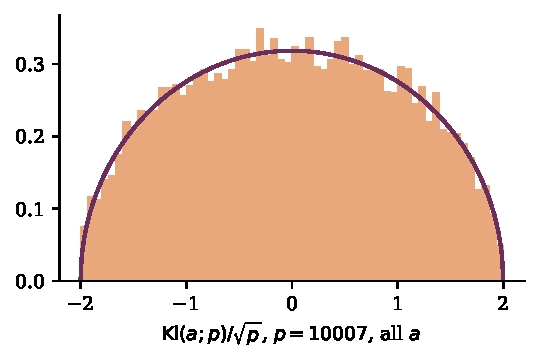
\includegraphics[width=0.62\textwidth]{figs/kloosterman_katz.pdf}
\caption{Histogram of the normalised Kloosterman sums $\mathrm{Kl}(a;p)/\sqrt p$ for all $a\in\mathbb{F}_p^\times$, $p=10007$, against the semicircle density $\frac1{2\pi}\sqrt{4-x^2}$ of $\ST$ (Theorem~\ref{thm:06bkatz}).}\label{fig:06bkatz}
\end{figure}

\subsection{The horizontal question}

For a fixed holomorphic newform of weight at least $2$ with trivial character and without complex multiplication, Sato Tate in the horizontal direction is a theorem (Theorem~\ref{thm:04STthm}), because the Satake parameters at varying $p$ are the local components of a single global automorphic representation, and the potential automorphy \cite{blght2011} and then automorphy \cite{newtonthorne2021,newtonthorne2021b} of its symmetric powers supply $L$ functions holomorphic and nonvanishing on $\Re s\ge1$ (Chapter~\ref{ch:04}). For Kloosterman sums there is no such global object: as $p$ varies, the sheaves $\mathcal{K}l$ live over different finite fields and are not known to be the reductions of a compatible system attached to a motive or automorphic representation over $\Q$. Katz conjectured the horizontal law nevertheless.

\begin{conjecture}[Katz's horizontal conjecture]\label{conj:06bhorizontal}\index{Katz horizontal conjecture}
Fix a nonzero integer $a$. As $p$ runs over the odd primes not dividing $a$, ordered by size, the angles $\theta_{p,a}$ are equidistributed in $[0,\pi]$ with respect to $\frac2\pi\sin^2\theta\,d\theta$. Equivalently,
\[
\frac{1}{\pi(x)}\sum_{p\le x,\ p\nmid a}U_n\Bigl(\frac{\mathrm{Kl}(a;p)}{2\sqrt p}\Bigr)\longrightarrow0\qquad(n\ge1).
\]
\end{conjecture}

Very little is known. Even the statement that $\mathrm{Kl}(1;p)$ is positive for infinitely many primes and negative for infinitely many primes is, to our knowledge, open; Fouvry and Michel proved sign changes of $\mathrm{Kl}(1;c)$ along moduli $c$ with a bounded number of prime factors \cite{fouvrymichel2007}, using sieve methods together with Katz's equidistribution results. The vertical theorem, by contrast with the horizontal conjecture, is geometry over a single finite field.

\section{Kloosterman sums and automorphic forms}\label{sec:06bkuznetsov}

For an integer $c\ge1$ let $S(m,n;c)=\sum_{x\in(\Z/c\Z)^\times}e((mx+n\bar x)/c)$. For prime $c=p$ this is $\mathrm{Kl}(m,n;p)$. The Chinese remainder theorem gives a twisted multiplicativity, and Weil's bound together with an elementary evaluation at prime powers yields
\[
|S(m,n;c)|\le\tau(c)\,(m,n,c)^{1/2}\,c^{1/2},
\]
with $\tau$ the divisor function \cite{iwanieckowalski2004}.

\subsection{The Bruggeman Kuznetsov formula}

Let $\{u_j\}$ be an orthonormal basis of Maass cusp forms for $\SL_2(\Z)$, eigenfunctions of the hyperbolic Laplacian with eigenvalues $\lambda_j=\frac14+t_j^2$, with Fourier expansions $u_j(z)=\sum_{n\ne0}\rho_j(n)W_{s_j}(nz)$, where $s_j=\frac12+it_j$ and $W_s(z)=2y^{1/2}K_{s-1/2}(2\pi y)e(x)$ is the Whittaker function, as in \cite{iwaniec2002}. Put $\nu_j(n)=(4\pi|n|/\cosh\pi t_j)^{1/2}\rho_j(n)$.

\begin{theorem}[Bruggeman \cite{bruggeman1978}, Kuznetsov \cite{kuznetsov1980}]\label{thm:06bkuznetsov}\index{Bruggeman Kuznetsov formula}
Let $\delta>0$ and let $h$ be even and holomorphic in $|\Im t|\le\frac12+\delta$ with $h(t)\ll(1+|t|)^{-2-\delta}$. For integers $m,n\ge1$,
\begin{multline*}
\sum_j h(t_j)\overline{\nu_j(m)}\nu_j(n)+\frac{1}{4\pi}\int_{-\infty}^{\infty}h(t)\,\overline{\eta_m(t)}\eta_n(t)\,dt\\
=\frac{\delta_{m,n}}{\pi}\int_{-\infty}^\infty t\tanh(\pi t)h(t)\,dt+\sum_{c\ge1}\frac{S(m,n;c)}{c}\,h^+\Bigl(\frac{4\pi\sqrt{mn}}{c}\Bigr),
\end{multline*}
where $\eta_n(t)=(4\pi|n|/\cosh\pi t)^{1/2}\rho_t(n)$, with $\rho_t(n)$ the coefficient of $W_{1/2+it}(nz)$ in the Eisenstein series $E(z,\frac12+it)$, and
\[
h^+(x)=2i\int_{-\infty}^\infty J_{2it}(x)\frac{h(t)\,t}{\cosh\pi t}\,dt .
\]
\end{theorem}

The normalisation of $W_s$, $\rho_j$, $\nu_j$ and of $E(z,s)=\sum_{\gamma\in\Gamma_\infty\backslash\SL_2(\Z)}\operatorname{Im}(\gamma z)^s$ is that of Iwaniec \cite{iwaniec2002}. Constants differ between sources: dividing by $\pi$ gives the equivalent form with spectral weights $\overline{a_j(m)}a_j(n)/\cosh\pi t_j$, where $a_j(n)=2|n|^{1/2}\rho_j(n)$ is the coefficient of $y^{1/2}K_{it_j}(2\pi|n|y)e(nx)$, diagonal constant $\pi^{-2}$ and prefactor $2i/\pi$ in $h^+$. The formula holds for congruence subgroups $\Gamma_0(N)$ with $c$ restricted to multiples of $N$. Its structure parallels the trace formula picture of Chapter~\ref{ch:07}. The left side is a spectral average of products of Fourier coefficients, that is of Hecke eigenvalues, since $\nu_j(n)=\nu_j(1)\lambda_j(n)$ for a basis of Hecke eigenforms, with $\lambda_j(n)$ the eigenvalues normalised so that the Ramanujan conjecture reads $|\lambda_j(p)|\le2$. The diagonal term $\delta_{m,n}$ carries the archimedean Plancherel density $t\tanh(\pi t)$, the analogue of the Kesten McKay density $\mu_q$, and the Kloosterman terms are the analogue of the cycle counts that measure the deviation of a finite quotient from its universal cover. The formula can be read in either direction: as a tool for averaging Fourier coefficients (the Kloosterman side is small by Weil), or as a tool for bounding sums of Kloosterman sums (the spectral side is controlled). The second reading is Kuznetsov's.

\subsection{Selberg's 3/16 theorem}

Let $\Gamma=\Gamma_0(N)$ and let $\lambda_1(\Gamma)$ be the smallest nonzero eigenvalue of the Laplacian on $L^2(\Gamma\backslash\mathbb{H})$. The continuous spectrum begins at $\frac14$, the bottom of the spectrum of the hyperbolic plane itself; an eigenvalue $\lambda=s(1-s)<\frac14$ with $\frac12<s<1$ is called exceptional.

\begin{theorem}[Selberg \cite{selberg1965}]\label{thm:06bselberg}\index{Selberg 3/16 theorem}
For every congruence subgroup $\Gamma_0(N)$, $\lambda_1\ge\frac{3}{16}$.
\end{theorem}

\paragraph{Sketch of Selberg's argument.} Consider the Kloosterman zeta function
\[
Z_{m,n}(s)=\sum_{c\equiv0\ (N)}\frac{S(m,n;c)}{c^{2s}} .
\]
Selberg showed, by unfolding the inner product of two Poincar\'e series and inserting the spectral decomposition, that $Z_{m,n}$ continues meromorphically, and that in $\Re s>\frac12$ its only possible poles are at the points $s_j\in(\frac12,1)$ with $s_j(1-s_j)$ an exceptional eigenvalue, with residue a nonzero multiple of $\sum\overline{\rho(m)}\rho(n)$ summed over an orthonormal basis of that eigenspace. Taking $m=n$ with $\rho(n)\ne0$ for some form in the eigenspace, the residue is a positive multiple of $\sum|\rho(n)|^2$, so the pole is genuine. On the other hand Weil's bound gives $|S(n,n;c)|\ll_{n,\varepsilon} c^{1/2+\varepsilon}$, so the series converges absolutely for $\Re s>\frac34$ and $Z_{n,n}$ is holomorphic there. Hence every exceptional $s_j$ satisfies $s_j\le\frac34$, and since $s\mapsto s(1-s)$ decreases on $[\frac12,1]$, $\lambda_j\ge\frac34\cdot\frac14=\frac3{16}$.

Selberg conjectured that $\lambda_1\ge\frac14$ for all congruence subgroups. In representation theoretic language this is the Ramanujan conjecture at the archimedean place for Maass forms: the archimedean component of the automorphic representation is tempered exactly when $\lambda\ge\frac14$. The best bound known is due to Kim and Sarnak in the appendix to Kim's paper \cite{kimsarnak2003}: using the automorphy of $\Sym^4$ for $\GL_2$, they show that the archimedean Satake parameter of a Maass cusp form on a congruence subgroup has real part at most $\frac7{64}$, hence $\lambda_1\ge\frac14-\bigl(\frac{7}{64}\bigr)^2=\frac{975}{4096}\approx0.238$. Earlier improvements on $\frac3{16}$ were obtained by Luo, Rudnick and Sarnak \cite{lrs1995} and by Kim and Shahidi \cite{kimshahidi2002}.

\subsection{Linnik and Selberg on sums of Kloosterman sums}

Weil's bound alone gives $\sum_{c\le x}|S(m,n;c)|/c\ll x^{1/2+\varepsilon}$. Linnik \cite{linnik1962} and Selberg \cite{selberg1965} conjectured that the signs of the Kloosterman sums cancel as $c$ varies.

\begin{conjecture}[Linnik, Selberg]\label{conj:06blinnik}\index{Linnik Selberg conjecture}
For fixed $m,n\ge1$ and every $\varepsilon>0$,
\[
\sum_{c\le x}\frac{S(m,n;c)}{c}\ll_{m,n,\varepsilon}x^{\varepsilon}.
\]
\end{conjecture}

Kuznetsov proved the bound $x^{1/6+\varepsilon}$ \cite{kuznetsov1980}, and to our knowledge the exponent $\frac16$ has not been improved for fixed $m,n$. He obtained it from the version of Theorem~\ref{thm:06bkuznetsov} read in the opposite direction, in which a test function on the Kloosterman side is prescribed (here one that approximates the indicator of $c\le x$) and the spectral side is bounded \cite{iwanieckowalski2004}. The connection with Theorem~\ref{thm:06bselberg} is direct. If the analogue of Conjecture~\ref{conj:06blinnik} held for $\Gamma_0(N)$, with $c$ restricted to multiples of $N$, then partial summation would make $Z_{n,n}(s)$ holomorphic in $\Re s>\frac12$, and Selberg's argument would exclude exceptional eigenvalues altogether. Conversely, an exceptional eigenvalue $s_j(1-s_j)$ produces a term of order $x^{2s_j-1}$ in the smoothed sums.

\paragraph{The probabilistic reading.} Think of $c\mapsto S(m,n;c)/\sqrt c$ as a sequence of random variables. For prime $c$ these are $2\cos\theta_{c,mn}$, and if the angles behaved like independent Sato Tate variables (the horizontal model of Conjecture~\ref{conj:06bhorizontal}) the sum $\sum_{p\le x}2\cos\theta_{p,mn}/\sqrt p$ would have mean zero and variance $\sum_{p\le x}1/p\sim\log\log x$, comfortably inside $x^\varepsilon$. Square root cancellation in sums of Kloosterman sums is therefore the statement that this sequence has no drift, and Theorem~\ref{thm:06bkuznetsov} identifies the possible drifts: they are the exceptional eigenvalues, each contributing a deterministic term $x^{2s_j-1}$. The analogy with Chapters~\ref{ch:07} and~\ref{ch:08} is close. There, a connected finite quotient of the tree is Ramanujan exactly when the return probabilities of simple random walk on it approach equilibrium at an exponential rate no slower than the Kesten rate $2\sqrt q/(q+1)$ (Proposition~\ref{prop:08three}); here, $\lambda_1\ge\frac14$ means that Brownian motion on $\Gamma\backslash\mathbb{H}$, with generator the Laplacian, mixes at least at the rate $e^{-t/4}$ dictated by the spectrum of the hyperbolic plane. In both settings the Ramanujan property is a spectral gap, and a trace formula converts it into cancellation in an arithmetic sum: counts of closed nonbacktracking walks in the first case, through the Ihara Bass formula, and Kloosterman sums over moduli in the second, through Kuznetsov's.

\section{Kloosterman paths}\label{sec:06bpaths}

Kowalski and Sawin \cite{kowalskisawin2016} asked what the partial sums of a Kloosterman sum look like. For $a\in\mathbb{F}_p^\times$ and $0\le t\le1$ let
\[
S_p(a,t)=\frac{1}{\sqrt p}\sum_{1\le x\le t(p-1)}e\Bigl(\frac{ax+\bar x}{p}\Bigr),
\]
and let $K_p(a,\cdot)\in C([0,1])$ be the polygonal path that interpolates linearly between the values at $t=j/(p-1)$, $0\le j\le p-1$. Then $K_p(a,0)=0$, $K_p(a,1)=\mathrm{Kl}(a;p)/\sqrt p$, and $|K_p(a,t)-S_p(a,t)|\le p^{-1/2}$, so the two have the same limiting finite dimensional distributions. With $a$ uniform in $\mathbb{F}_p^\times$, $K_p$ is a random continuous function.\index{Kloosterman path}

\begin{definition}\label{def:06bK}
Let $(\mathrm{ST}_h)_{h\in\Z}$ be independent random variables with law $\ST$ and put $c_0(t)=t$ and $c_h(t)=(e(ht)-1)/(2\pi ih)$ for $h\ne0$. The \emph{Kloosterman random Fourier series} is
\[
K(t)=\sum_{h\in\Z}c_h(t)\,\mathrm{ST}_h=t\,\mathrm{ST}_0+\sum_{h\ne0}\frac{e(ht)-1}{2\pi ih}\mathrm{ST}_h ,
\]
the series being the limit of its symmetric partial sums over $|h|\le H$ as $H\to\infty$.
\end{definition}

Since $\E\,\mathrm{ST}_h=0$, $\E\,\mathrm{ST}_h^2=1$ and $\sum_h|c_h(t)|^2<\infty$, the series converges in $L^2$ and almost surely for each $t$. Kowalski and Sawin show, with Kahane's theory of random Fourier series, that $K$ is almost surely continuous, indeed H\"older continuous of every order below $\frac12$, and almost surely nowhere differentiable \cite{kowalskisawin2016}; so $K$ is a random element of $C([0,1])$. Since $c_h(t)=\int_0^te(hu)\,du$, the process $K$ is formally the integral $\int_0^tW(u)\,du$ of the random Fourier series $W(u)=\sum_h\mathrm{ST}_he(hu)$, whose Fourier coefficients are independent Sato Tate variables. Equivalently $c_h(t)=\overline{\widehat{\mathbb{I}_{[0,t]}}(h)}$, where $\hat f(h)=\int_0^1f(u)e(-hu)\,du$, and in this form the coefficients arise from the discrete Fourier analysis of an interval, as we now show.

\subsection{The completion formula}

\begin{lemma}[Completion]\label{lem:06bcompletion}\index{completion method}
Let $I=\{1,\dots,m\}$ with $m=\lfloor t(p-1)\rfloor$ and, for $h\in\Z$,
\[
\alpha_p(h,t)=\frac1p\sum_{y=1}^me\Bigl(\frac{hy}{p}\Bigr).
\]
Then, for every $a\in\mathbb{F}_p$,
\begin{equation}\label{eq:06bcompletion}
S_p(a,t)=\sum_{|h|<p/2}\alpha_p(h,t)\,\frac{\mathrm{Kl}(a-h;p)}{\sqrt p}.
\end{equation}
Further $\alpha_p(0,t)=m/p$, $|\alpha_p(h,t)|\le 1/(2|h|)$ for $1\le|h|<p/2$, and $\alpha_p(h,t)\to c_h(t)$ as $p\to\infty$ for each fixed $h$ and $t$.
\end{lemma}

\begin{proof}
By finite Fourier inversion on $\Z/p\Z$, for every residue $x$,
\[
\mathbb{I}_I(x)=\sum_{h\bmod p}\alpha_p(h,t)\,e\Bigl(-\frac{hx}{p}\Bigr),
\]
since $\sum_h\alpha_p(h,t)e(-hx/p)=p^{-1}\sum_{y\in I}\sum_he(h(y-x)/p)$ and the inner sum is $p$ when $y=x$ and $0$ otherwise. Insert this into the definition of $S_p$ and interchange the sums:
\begin{align*}
\sqrt p\,S_p(a,t)&=\sum_{h\bmod p}\alpha_p(h,t)\sum_{x\in\mathbb{F}_p^\times}e\Bigl(\frac{(a-h)x+\bar x}{p}\Bigr)\\
&=\sum_{h\bmod p}\alpha_p(h,t)\,\mathrm{Kl}(a-h;p);
\end{align*}
then represent the residues $h$ by $|h|<p/2$. For $h\ne0$ the geometric sum gives $|\sum_{y=1}^me(hy/p)|=|\sin(\pi hm/p)/\sin(\pi h/p)|\le1/|\sin(\pi h/p)|$, and $\sin(\pi u)\ge2u$ for $0\le u\le\frac12$ gives $|\alpha_p(h,t)|\le 1/(2|h|)$. Finally $\alpha_p(h,t)$ is a Riemann sum for $\int_0^{m/p}e(hu)\,du$ with mesh $1/p$, and $m/p\to t$, so $\alpha_p(h,t)\to\int_0^te(hu)\,du=c_h(t)$.
\end{proof}

Formula \eqref{eq:06bcompletion} is the starting point of Kowalski and Sawin \cite{kowalskisawin2016}. Its term $h\equiv a$ involves $\mathrm{Kl}(0;p)=-1$; it is the only one that is not a genuine Kloosterman sum, and for $1\le a\le p-1$ its coefficient is at most $1/(2\min(a,p-a))$ in absolute value. The completion formula exhibits the path as a linear functional of the shifted sums $\mathrm{Kl}(a-h;p)$, $|h|<p/2$, which by Theorem~\ref{thm:06bjoint} are asymptotically independent Sato Tate variables. Renaming $h\mapsto-h$ writes the same identity with the shifts $\mathrm{Kl}(a+h;p)$ and the limiting coefficients $c_{-h}(t)$; the law of $K$ is unchanged because the $\mathrm{ST}_h$ are independent and identically distributed.

The next lemma controls the tail of \eqref{eq:06bcompletion} uniformly in $p$; it uses only orthogonality.

\begin{lemma}[Uniform tail bound; this book]\label{lem:06btail}
For every $H\ge1$, every $p>2H+1$ and every $t\in[0,1]$,
\[
\frac{1}{p-1}\sum_{a\in\mathbb{F}_p^\times}\Bigl|\sum_{H<|h|<p/2}\alpha_p(h,t)\frac{\mathrm{Kl}(a-h;p)}{\sqrt p}\Bigr|^2\le\frac1H .
\]
\end{lemma}

\begin{proof}
For $k\in\mathbb{F}_p$, orthogonality in $c$ gives
\begin{align*}
\sum_{c\in\mathbb{F}_p}\mathrm{Kl}(c;p)\mathrm{Kl}(c+k;p)&=\sum_{x,y\ne0}e\Bigl(\frac{\bar x+\bar y+ky}{p}\Bigr)\sum_ce\Bigl(\frac{c(x+y)}{p}\Bigr)\\
&=p\sum_{x\ne0}e\Bigl(-\frac{kx}{p}\Bigr),
\end{align*}
which is $p(p-1)$ for $k=0$ and $-p$ for $k\ne0$. Hence, since the $\mathrm{Kl}(c;p)$ are real, for any coefficients $\beta_h$ indexed by a set $\mathcal{H}$ of distinct residues,
\[
\frac1p\sum_{c\in\mathbb{F}_p}\Bigl|\sum_{h\in\mathcal{H}}\beta_h\frac{\mathrm{Kl}(c-h;p)}{\sqrt p}\Bigr|^2=\sum_{h}|\beta_h|^2-\frac1p\Bigl|\sum_h\beta_h\Bigr|^2,
\]
which is at most $\sum_h|\beta_h|^2$. Take $\mathcal{H}=\{H<|h|<p/2\}$ and $\beta_h=\alpha_p(h,t)$. By Lemma~\ref{lem:06bcompletion}, $\sum_{|h|>H}|\alpha_p(h,t)|^2\le2\sum_{h>H}\frac1{4h^2}\le\frac1{2H}$. Passing from $\mathbb{F}_p$ to $\mathbb{F}_p^\times$ multiplies the average of a nonnegative quantity by at most $p/(p-1)\le2$.
\end{proof}

\begin{theorem}[Kowalski and Sawin \cite{kowalskisawin2016}]\label{thm:06bks}
With $a$ uniform in $\mathbb{F}_p^\times$, the finite dimensional distributions of the Kloosterman paths $K_p(a,\cdot)$ converge to those of $K$: for all $0\le t_1<\dots<t_k\le1$, $(K_p(a,t_i))_{i\le k}\Rightarrow(K(t_i))_{i\le k}$ in $\C^k$.
\end{theorem}

\begin{proof}[Proof, given Theorem~\ref{thm:06bjoint}]
It suffices to treat $S_p(a,t_i)$. Fix $H$ and let $S^{(H)}_p(a,t)$ be the part of \eqref{eq:06bcompletion} with $|h|\le H$, and $K^{(H)}(t)=\sum_{|h|\le H}c_h(t)\mathrm{ST}_h$. Excluding the at most $2H+1$ values $a\equiv h$, Theorem~\ref{thm:06bjoint} gives $(\mathrm{Kl}(a-h;p)/\sqrt p)_{|h|\le H}\Rightarrow(\mathrm{ST}_h)_{|h|\le H}$, and these vectors lie in the compact cube $[-2,2]^{2H+1}$ by Weil's bound. The vector $(S^{(H)}_p(a,t_i))_i$ is the image of this vector under a linear map whose coefficients $\alpha_p(h,t_i)$ converge to $c_h(t_i)$ (Lemma~\ref{lem:06bcompletion}), so $(S^{(H)}_p(a,t_i))_i\Rightarrow(K^{(H)}(t_i))_i$ as $p\to\infty$. Next, $(K^{(H)}(t_i))_i\to(K(t_i))_i$ in $L^2$ as $H\to\infty$, because $\sum_{|h|>H}|c_h(t)|^2\le\sum_{|h|>H}\pi^{-2}h^{-2}\le 2/(\pi^2H)$. Finally, by Lemma~\ref{lem:06btail}, Chebyshev's inequality and a union bound, $\Prob(\max_i|S_p(a,t_i)-S^{(H)}_p(a,t_i)|>\varepsilon)\le k/(H\varepsilon^2)$ for all $p>2H+1$. The approximation theorem for weak convergence \cite[Theorem~4.2]{billingsley1968} now gives the claim.
\end{proof}

Thus Katz's joint equidistribution, which is the deep input, enters only through finitely many shifts at a time, and the infinite series is assembled by an $L^2$ argument that needs nothing beyond orthogonality of additive characters.

\paragraph{Tightness.} Convergence in law in $C([0,1])$ requires in addition tightness, for instance a moment bound of the form $\E|K_p(a,t)-K_p(a,s)|^4\ll|t-s|^{1+\delta}$ uniformly in $p$, which amounts to square root cancellation in \emph{short} Kloosterman sums averaged over $a$. Kowalski and Sawin prove convergence in law in $C([0,1])$ in two cases where such an estimate is available \cite{kowalskisawin2016}: the two parameter family $\sum_{x}e((ax+b\bar x)/p)$ with $(a,b)$ uniform in $(\mathbb{F}_p^\times)^2$ (they phrase it as an extra average over the additive character), where the extra average supplies the fourth moment bound, and the Birch sums $\sum_xe((ax+x^3)/p)$. For the one parameter family above the required estimate for short sums averaged over $a$ alone is not known, and they explain that convergence in $C([0,1])$ would follow from natural conjectures on short sums. In later work they describe the support of the limiting law in $C([0,1])$ \cite{kowalskisawin2017}.

\subsection{Exact second moments and the convention lesson}

The second moments of the paths can be computed exactly at every finite $p$, without Katz's theorem. Let $I=\{1,\dots,m\}$ be the interval of Lemma~\ref{lem:06bcompletion} and $-I=\{p-x:x\in I\}$.

\begin{proposition}[Second moments of Kloosterman paths; this book]\label{prop:06bsecond}
Let $R_I=\sum_{x\in I}e(\bar x/p)$ and $G_I=\sum_{x\in I}e(x/p)$. With $a$ uniform in $\mathbb{F}_p^\times$:
\begin{enumerate}
\item for $S_p(a,t)=p^{-1/2}\sum_{x\in I}e((ax+\bar x)/p)$,
\[
\E|S_p|^2=\frac{p|I|-|R_I|^2}{p(p-1)},\qquad\E S_p^2=\frac{p\,|I\cap(-I)|-R_I^2}{p(p-1)};
\]
\item for $S'_p(a,t)=p^{-1/2}\sum_{x\in I}e((x+a\bar x)/p)$,
\[
\E|S'_p|^2=\frac{p|I|-|G_I|^2}{p(p-1)},\qquad\E S_p'^2=\frac{p\,|I\cap(-I)|-G_I^2}{p(p-1)}.
\]
\end{enumerate}
In both cases $\E S=-p^{-1/2}(p-1)^{-1}R_I$, respectively $-p^{-1/2}(p-1)^{-1}G_I$, which tends to $0$.
\end{proposition}

\begin{proof}
For the first family, summing over all $a\in\mathbb{F}_p$,
\[
\sum_a\Bigl|\sum_{x\in I}e\Bigl(\frac{ax+\bar x}{p}\Bigr)\Bigr|^2=\sum_{x,y\in I}e\Bigl(\frac{\bar x-\bar y}{p}\Bigr)\sum_ae\Bigl(\frac{a(x-y)}{p}\Bigr)=p|I|,
\]
and similarly $\sum_a(\sum_{x\in I}e((ax+\bar x)/p))^2=p\sum_{x,y\in I,\,x+y\equiv0}e((\bar x+\bar y)/p)=p|I\cap(-I)|$, because $\bar y=-\bar x$ when $y=-x$. Removing the term $a=0$, which equals $R_I$, and dividing by $p(p-1)$ gives (1). The second family is identical with the roles of $x$ and $\bar x$ exchanged in the orthogonality step; now the term $a=0$ is the geometric sum $G_I$. The means follow from $\sum_{a\in\mathbb{F}_p}e(a\bar x/p)=\sum_ae(ax/p)=0$ for $x\ne0$, and $|R_I|\le p$, $|G_I|\le p$.
\end{proof}

The two families have the same complete sums, since $\mathrm{Kl}(a,1)=\mathrm{Kl}(1,a)$, and the same variance over all $a\in\mathbb{F}_p$. They differ only through the single excluded value $a=0$, and that value matters in exactly one of them. In the first family $R_I$ is an incomplete Kloosterman sum, and the completion method gives $|R_I|\ll\sqrt p\log p$, so $|R_I|^2/p^2\to0$. In the second family $G_I$ is a geometric sum of size comparable to $p$: $G_I/p\to\int_0^te(u)\,du=c_1(t)$. Therefore, as $p\to\infty$,
\begin{gather*}
\E|S_p|^2\to t,\qquad\E S_p^2\to(2t-1)_+,\\
\E|S'_p|^2\to t-|c_1(t)|^2,\qquad\E S_p'^2\to(2t-1)_+-c_1(t)^2 .
\end{gather*}

The same phenomenon is visible in the completion formula. Expanding $\mathbb{I}_I$ as in Lemma~\ref{lem:06bcompletion} in the second family gives
\begin{align*}
\sqrt p\,S'_p(a,t)&=\sum_{h\bmod p}\alpha_p(h,t)\sum_{x\ne0}e\Bigl(\frac{(1-h)x+a\bar x}{p}\Bigr)\\
&=\sum_{h\not\equiv1}\alpha_p(h,t)\,\mathrm{Kl}\bigl(a(1-h);p\bigr)-\alpha_p(1,t),
\end{align*}
because for $h=1$ the inner sum is the Ramanujan sum $\sum_{x\ne0}e(a\bar x/p)=-1$. After division by $\sqrt p$ the term $h=1$ is $O(p^{-1/2})$: the Sato Tate variable that should carry the coefficient $c_1(t)$ is simply absent, and the remaining coefficients multiply Kloosterman sums at the multiplicative translates $a(1-h)$. Kowalski and Sawin point this out in a remark of \cite{kowalskisawin2016}, where the shifts are written $a(1+h)$ and the missing index is $h=-1$, and they show that in this parametrisation the paths do converge in law in $C([0,1])$, because here the short sum estimate needed for tightness follows from a counting result of Bourgain and Garaev; the limit is $K-c_1\mathrm{ST}_1$ in our notation. Their displayed formula has $c_{-1}\mathrm{ST}_{-1}$ in place of $c_1\mathrm{ST}_1$, a process with the law of the complex conjugate of $K-c_1\mathrm{ST}_1$; with the conventions of Lemma~\ref{lem:06bcompletion} the missing coefficient is $c_1$, as the limit of $\E S_p'^2$ above shows, because $c_1(t)^2$ is not real for $0<t<1$, $t\ne\frac12$. Proposition~\ref{prop:06bsecond} confirms, unconditionally and at every finite $p$, that the second order structure is that of $K-c_1\mathrm{ST}_1$, and not that of $K$.

\begin{corollary}[Variance deficit; this book]\label{cor:06bdeficit}
In the parametrisation $e((x+a\bar x)/p)$ the limiting variances are
\begin{gather*}
\mathrm{Var}\,\Re S'=\tfrac12\bigl(t+(2t-1)_+\bigr)-\frac{\sin^2(2\pi t)}{4\pi^2},\\
\mathrm{Var}\,\Im S'=\tfrac12\bigl(t-(2t-1)_+\bigr)-\frac{\sin^4(\pi t)}{\pi^2}.
\end{gather*}
At $t=\frac12$ the real part is unaffected and the imaginary part loses exactly $1/\pi^2$: $\mathrm{Var}\,\Im S'\to\frac14-\frac1{\pi^2}=0.1487$.
\end{corollary}

\begin{proof}
Write $c_1(t)=\frac{\sin2\pi t}{2\pi}+i\frac{1-\cos2\pi t}{2\pi}$, so $(\Re c_1)^2=\sin^2(2\pi t)/(4\pi^2)$ and $(\Im c_1)^2=\sin^4(\pi t)/\pi^2$. Since the means tend to zero, $\mathrm{Var}\,\Re S'=\frac12(\E|S'|^2+\Re\E S'^2)$ and $\mathrm{Var}\,\Im S'=\frac12(\E|S'|^2-\Re\E S'^2)$; insert the limits above and use $|c|^2\pm\Re c^2=2(\Re c)^2$ or $2(\Im c)^2$.
\end{proof}

Our first run of the path computations, at $p=10007$, used the parametrisation $e((x+a\bar x)/p)$, natural for the vertical statistics of Section~\ref{sec:06bkatz}. It gave $\mathrm{Var}\,\Im S'(\frac12)=0.149$, where the random Fourier series sample of that run gave $0.258$. Corollary~\ref{cor:06bdeficit} explains the gap: the limiting value is $\frac14-\frac1{\pi^2}=0.1487$, a deficit of $1/\pi^2=0.101$ against the value $\frac14$ for $K$. At $p=1009$ and $t=\frac12$, the exact formulas of Proposition~\ref{prop:06bsecond}, averaged over all $a$, give $0.14848$, against $\frac14-\frac1{\pi^2}=0.14868$. The lesson is general: vertical statistics of a complete sum are blind to the parametrisation, but partial sums are not, and a single Ramanujan sum can remove one independent coordinate of the limit.

\subsection{Numerical check}

For $p=10007$ and $3000$ random $a$ we compared the paths $K_p(a,\cdot)$, in the parametrisation of Kowalski and Sawin, with $4000$ samples of the random Fourier series truncated at $|h|\le3000$. Two sample Kolmogorov Smirnov tests give the following $p$ values for the real and imaginary parts: at $t=\frac14$, $0.79$ and $0.80$; at $t=\frac12$, $0.82$ and $0.77$; at $t=\frac34$, $0.70$ and $0.80$. At $t=\frac12$ the variances are $0.2502$ (paths) and $0.2529$ (series) for the real part and $0.2459$ and $0.2463$ for the imaginary part, against the value $\frac14$ for both from Proposition~\ref{prop:06bcov} below. For the sup norm $\|K_p\|_\infty$ the means are $1.159$ and $1.138$, with a two sample Kolmogorov Smirnov $p$ value of $0.16$. The sup norm is not a finite dimensional functional, so this agreement is consistent with convergence in law in $C([0,1])$ for the one parameter family, the part of the theory that is not proved. Figure~\ref{fig:06bpaths} shows typical paths. At $p=1009$, averaging over all $a$, the exact formulas of Proposition~\ref{prop:06bsecond} give $\mathrm{Var}\,\Re S_p(\frac12)=0.25000$ and $\mathrm{Var}\,\Im S_p(\frac12)=0.24992$.

\begin{figure}[t]\centering
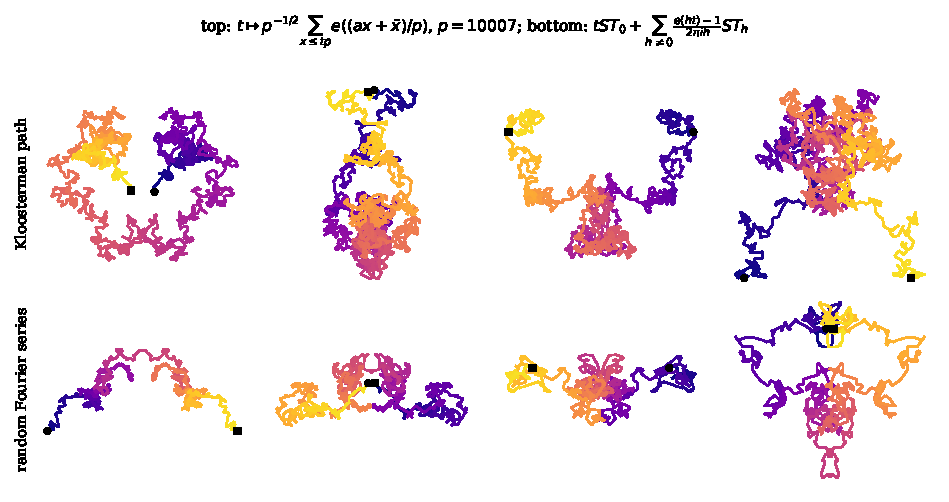
\includegraphics[width=\textwidth]{figs/kloosterman_paths.pdf}
\caption{Top: Kloosterman paths $t\mapsto p^{-1/2}\sum_{x\le t(p-1)}e((ax+\bar x)/p)$ in the complex plane for four values of $a$, $p=10007$, coloured by $t$. Bottom: four samples of the random Fourier series $K(t)$ of Definition~\ref{def:06bK}. Every path starts at $0$ and ends on the real axis at a point of $[-2,2]$; its imaginary part is symmetric about $t=\frac12$, and the path is symmetric under reflection in the vertical line through the midpoint of its endpoints (Proposition~\ref{prop:06bcov}).}\label{fig:06bpaths}
\end{figure}

\subsection{Properties of the limit}

\begin{proposition}[Covariance and symmetry of $K$; this book]\label{prop:06bcov}\index{random Fourier series}
For $s,t\in[0,1]$,
\[
\E\,K(s)\overline{K(t)}=\min(s,t),\qquad\E\,K(s)K(t)=(s+t-1)_+ .
\]
Consequently $\mathrm{Var}\,\Re K(t)=\frac12\bigl(t+(2t-1)_+\bigr)$, $\mathrm{Var}\,\Im K(t)=\frac12\bigl(t-(2t-1)_+\bigr)$, and $\Re K(t)$, $\Im K(t)$ are uncorrelated. Moreover, almost surely,
\[
K(1-t)=K(1)-\overline{K(t)}\qquad(0\le t\le1),
\]
so $\Im K(1-t)=\Im K(t)$, $K(1)=2\Re K(\frac12)=\mathrm{ST}_0$, and $\Im K(0)=\Im K(1)=0$.
\end{proposition}

\begin{proof}
Since the $\mathrm{ST}_h$ are independent, real, centred and of variance one, $\E K(s)\overline{K(t)}=\sum_hc_h(s)\overline{c_h(t)}$ and $\E K(s)K(t)=\sum_hc_h(s)c_h(t)$. With $f=\mathbb{I}_{[0,s]}$ and $g=\mathbb{I}_{[0,t]}$ we have $c_h(s)=\overline{\hat f(h)}$, so Parseval gives $\sum_h\overline{\hat f(h)}\hat g(h)=\int_0^1fg=\min(s,t)$. For the second identity, $\hat g(h)=\overline{\hat{\tilde g}(h)}$ with $\tilde g(u)=g(-u)$ on $\R/\Z$, so $\sum_h\overline{\hat f(h)}\,\overline{\hat g(h)}=\sum_h\overline{\hat f(h)}\hat{\tilde g}(h)=\int_0^1f(u)g(-u)\,du$, the length of $[0,s]\cap[1-t,1]$, which is $(s+t-1)_+$. Both sums are real, so the variances follow from $\mathrm{Var}\,\Re K=\frac12(\E|K|^2+\E K^2)$ and $\mathrm{Var}\,\Im K=\frac12(\E|K|^2-\E K^2)$, and the covariance of the real and imaginary parts is $\frac12\Im\E K^2=0$. For the symmetry, $e(h(1-t))=e(-ht)$ gives $c_h(1-t)=-\overline{c_h(t)}$ for $h\ne0$ and $c_h(1)=0$; summing term by term, $K(1-t)=(1-t)\mathrm{ST}_0-\overline{(K(t)-t\,\mathrm{ST}_0)}=\mathrm{ST}_0-\overline{K(t)}$, and $K(1)=\mathrm{ST}_0$.
\end{proof}

At $t=\frac14$ the formulas of Proposition~\ref{prop:06bcov} give $\frac18$ and $\frac18$, against the observed path variances $0.1234$ and $0.1249$, and at $t=\frac34$ they give $\frac58$ and $\frac18$, against $0.6308$ and $0.1249$; the two observed imaginary variances coincide, as the symmetry below forces already at finite $p$. The limits of the exact second moments in Proposition~\ref{prop:06bsecond}, $\E|S_p|^2\to t$ and $\E S_p^2\to(2t-1)_+$, are exactly these covariances at $s=t$, and the same computation with two intervals gives $\min(s,t)$ and $(s+t-1)_+$ for $s\ne t$: the second order structure of the paths agrees with that of $K$ unconditionally, without Katz's theorem.

The arithmetic meaning of the symmetry is simple: $x\mapsto p-x$ maps $e((ax+\bar x)/p)$ to its conjugate, so $K_p(a,1-t)=K_p(a,1)-\overline{K_p(a,t)}$ for all $t$. The second half of a Kloosterman path is therefore the mirror image of the first half in the vertical line $\Re z=\mathrm{Kl}(a;p)/(2\sqrt p)$, which is the symmetry visible in every path of Figure~\ref{fig:06bpaths}.

\begin{proposition}[Unboundedness and a Gaussian tail bound; this book]\label{prop:06btail}
The random variable $\Im K(\frac12)=\frac1\pi\sum_{h\ \mathrm{odd}}\mathrm{ST}_h/h$ is unbounded above and below, and for every $M>0$,
\[
\Prob\bigl(\Im K(\tfrac12)>M\bigr)\le e^{-2M^2},
\]
the Chernoff bound of a centred Gaussian variable with the same variance $\frac14$. More generally, every real random variable $X=\sum_h\gamma_h\mathrm{ST}_h$ with $\sum_h\gamma_h^2<\infty$, in particular every real linear combination of the real and imaginary parts of finitely many values of $K$, satisfies $\E e^{\lambda X}\le e^{\lambda^2\mathrm{Var}(X)/2}$ for all real $\lambda$.
\end{proposition}

\begin{proof}
At $t=\frac12$, $c_h=((-1)^h-1)/(2\pi ih)$ vanishes for even $h\ne0$ and equals $i/(\pi h)$ for odd $h$, which gives the formula; pairing $h$ with $-h$, $\Im K(\frac12)=\frac1\pi\sum_{h>0\ \mathrm{odd}}(\mathrm{ST}_h-\mathrm{ST}_{-h})/h$. Given $M$, choose $N$ with $\frac{3}{\pi}\sum_{h\le N,\ h\ \mathrm{odd}}\frac1h>M+1$, possible since the harmonic series over odd integers diverges. With positive probability $\mathrm{ST}_h>1.5$ and $\mathrm{ST}_{-h}<-1.5$ for all odd $h\le N$, so the partial sum exceeds $M+1$. The remainder is independent of this event and symmetric, so it is nonnegative with probability at least $\frac12$. Hence $\Prob(\Im K(\frac12)>M+1)>0$, and the law is symmetric. For the tail, the law $\ST$ is subgaussian with variance proxy equal to its variance: its odd moments vanish and its even moments are the Catalan numbers $C_k=(2k)!/(k!\,(k+1)!)$, so
\[
\E e^{\lambda\mathrm{ST}_h}=\sum_{k\ge0}\frac{\lambda^{2k}}{k!\,(k+1)!}\le\sum_{k\ge0}\frac{\lambda^{2k}}{2^kk!}=e^{\lambda^2/2},
\]
because $2^k\le(k+1)!$. For $X=\sum_h\gamma_h\mathrm{ST}_h$, independence gives $\E e^{\lambda X_N}\le e^{\lambda^2\sum_{|h|\le N}\gamma_h^2/2}$ for the partial sums $X_N$, which converge to $X$ almost surely, and Fatou's lemma gives $\E e^{\lambda X}\le e^{\lambda^2\mathrm{Var}(X)/2}$, since $\mathrm{Var}(X)=\sum_h\gamma_h^2$. For $\Im K(\frac12)$ we have $\gamma_h=1/(\pi h)$ for odd $h$ and $\sum_{h\ \mathrm{odd}}\gamma_h^2=\frac{2}{\pi^2}\cdot\frac{\pi^2}{8}=\frac14$, and Chernoff's bound with $\lambda=4M$ gives $\Prob(\Im K(\frac12)>M)\le e^{-4M^2+2M^2}=e^{-2M^2}$.
\end{proof}

So although each normalised Kloosterman sum lies in $[-2,2]$, the limit of the partial sums is unbounded, consistent with the fact that partial sums of such exponential sums can be as large as a constant times $\sqrt p\log\log p$; for Birch sums Lamzouri showed that some partial sum reaches $(\frac2\pi+o(1))\sqrt p\log\log p$ \cite{lamzouri2020}. The true tails are much thinner than Gaussian. Kowalski and Sawin prove that for $0<t<1$ there is $c=c(t)>0$ with
\[
c^{-1}\exp\bigl(-\exp(cM)\bigr)\le\Prob\bigl(|\Im K(t)|\ge M\bigr)\le c\exp\bigl(-\exp(M/c)\bigr)\quad(M>0),
\]
the same bounds for $|\Re K(t)|$ when $t\ne\frac12$, and bounds of the same shape for $\|K\|_\infty$ \cite{kowalskisawin2016}. For the maximum of the partial sums at finite $p$, Lamzouri obtained nearly matching bounds of this type for Birch sums \cite{lamzouri2020}, and Autissier, Bonolis and Lamzouri showed, for Birch sums and for the two parameter Kloosterman family, that the proportion of parameters for which the maximum exceeds $V\sqrt p$ is $\exp(-\exp(\pi V/2+O(1)))$, uniformly for $V$ up to about $\frac2\pi\log\log p$; for the further families of trace functions that they treat, whose normalised Fourier transforms take values in $[-N,N]$, they prove the same with $\frac\pi2$ replaced by $\frac\pi N$ and the range by $\frac N\pi\log\log p$ \cite{abl2021}.

\section{Probabilistic interpretation}\label{sec:06bprob}

\paragraph{A Sato Tate Brownian motion.} Proposition~\ref{prop:06bcov} says that on $[0,\frac12]$ the process $K$ has exactly the second order structure of a standard complex Brownian motion $Z$: $\E K(s)\overline{K(t)}=\min(s,t)$ and $\E K(s)K(t)=0$ for $s,t\le\frac12$. On $[\frac12,1]$ it is determined by its first half through the reflection $K(t)=2\Re K(\frac12)-\overline{K(1-t)}$. The Gaussian process with the same covariance is therefore complex Brownian motion on $[0,\frac12]$ folded back on itself: the imaginary part is a Brownian path on $[0,\frac12]$ followed by its time reversal, so it is pinned at $0$ at both ends like a bridge, and the real part is a Brownian path followed by its reflection through the midpoint value, ending at $2\Re Z(\frac12)$, a centred Gaussian of variance one. The Kloosterman process differs from this Gaussian model in two visible ways. Its endpoint $K(1)=\mathrm{ST}_0$ is semicircular, hence bounded, and its marginals are not Gaussian although their tails are subgaussian (Proposition~\ref{prop:06btail}), indeed doubly exponential. The three processes are one series with three choices of coefficients. With independent standard complex Gaussian coefficients ($\E|\zeta_h|^2=1$, $\E\zeta_h^2=0$) the series $\sum_hc_h(t)\zeta_h$ is a centred complex Gaussian process with covariances $\min(s,t)$ and $0$, by the proof of Proposition~\ref{prop:06bcov}, that is, a standard complex Brownian motion on $[0,1]$; with independent real standard Gaussian coefficients it is the folded process just described (Exercise~\ref{ex:06bgauss}); and with independent real Sato Tate coefficients, the traces of independent Haar elements of $\SU(2)$, it is $K$. In this sense $K$ is a Sato Tate Brownian motion.

\paragraph{Relation to random matrices.} Writing $\mathrm{ST}_h=\tr g_h$ with $g_h$ independent Haar elements of $\SU(2)$, the limit is a linear statistic of an infinite sequence of independent random matrices. Other one variable sums lead to other groups. For the additive twists $x\mapsto\mathrm{Kl}^{(r)}(\overline{ax};p)\,e(bx/p)$ of the hyper Kloosterman sums $\mathrm{Kl}^{(r)}(c;p)=\sum_{y_1\cdots y_r=c}e((y_1+\dots+y_r)/p)$, the discrete Fourier transforms are, after normalisation, the hyper Kloosterman sums $\mathrm{Kl}^{(r+1)}(\bar a(b+h);p)$ for $h\ne-b$, so Katz's monodromy computation makes the coefficients of the limit traces of Haar elements of $\USp(r+1)$ when $r$ is odd; for odd $r\ge3$ these are among the families of Autissier, Bonolis and Lamzouri recalled in Section~\ref{sec:06bpaths}, with $N=r+1$. For prime power moduli Ricotta and Royer found a limit of the same shape whose coefficients have an atom of mass $\frac12$ at $0$ and an arcsine part \cite{ricottaroyer2018}. This law is the measure $\mu_{\mathrm{CM}}$ of elliptic curves with complex multiplication (Chapter~\ref{ch:04}), because Kloosterman sums to prime power moduli have an elementary evaluation: for odd $p$, modulus $p^k$ with $k\ge2$ and parameters prime to $p$, they vanish unless the product of the parameters is a square modulo $p$, and are otherwise, up to sign, $p^{k/2}$ times twice the cosine of an explicit angle.

\paragraph{Open questions.} We record four.
\begin{enumerate}
\item The law of $\|K\|_\infty$ is not known in closed form. Autissier, Bonolis and Lamzouri determine its tail up to the constant in the exponent, $\Prob(\|K\|_\infty>V)=\exp(-\exp(\pi V/2+O(1)))$ for large $V$ \cite{abl2021}, but the distribution function, and even its mean ($1.138$ in our simulation), have no formula.
\item Extreme values. In the two parameter family the normalised maximum of the partial sums is $O(\log p)$ for every $(a,b)$ by the completion method, and exceeds $(\frac2\pi+o(1))\log\log p$ for many $(a,b)$ \cite{abl2021}. Whether it is $O(\log\log p)$ for all $(a,b)$, which is what the estimate of Autissier, Bonolis and Lamzouri would give if it held for all $V$, is open; they show that the corresponding bound fails for some families of periodic functions to which their theorem applies, although these families, unlike Kloosterman sums, are not uniformly bounded.
\item For the one parameter family, convergence in law in $C([0,1])$ depends on estimates for short Kloosterman sums averaged over the parameter that are not known (see the discussion of tightness above).
\item Horizontal paths. Fix an integer $a\ne0$ and let $p$ be uniform among the primes up to $x$. Do the paths $K_p(a,\cdot)$ converge in finite dimensional distributions, as $x\to\infty$, to $K-c_a\mathrm{ST}_a$? For fixed $a$ the term $h=a$ of \eqref{eq:06bcompletion} is $-\alpha_p(a,t)/\sqrt p$, so one Sato Tate coefficient disappears, as in the second parametrisation. The endpoint $K_p(a,1)=2\cos\theta_{p,a}$ alone is the subject of Conjecture~\ref{conj:06bhorizontal}, and the finite dimensional distributions would also need the angles $\theta_{p,a-h}$ at distinct shifts $h\ne a$ to become independent as $p$ varies.
\end{enumerate}

\section{Notes}

Kloosterman introduced his sums in 1926 to treat quaternary quadratic forms by the circle method, obtaining a bound of order $p^{3/4}$ \cite{kloosterman1926}. Weil's paper \cite{weil1948b} deduced $2\sqrt p$ from his proof of the Riemann hypothesis for curves over finite fields \cite{weil1948}; Stepanov's method \cite{stepanov1969}, in Bombieri's formulation \cite{bombieri1974}, gives an elementary proof. The theory of Kloosterman sheaves, their monodromy, and the equidistribution theorem are in Katz's monograph \cite{katz1988}; Deligne's equidistribution theorem is in Weil II \cite{deligne1980}, and the Goursat Kolchin Ribet criterion is in \cite{katz1990}. Katz and Sarnak \cite{katzsarnak1999} develop the general passage from monodromy to random matrices used in Chapter~\ref{ch:06}. Iwaniec and Kowalski \cite{iwanieckowalski2004} treat exponential sums over finite fields, Kloosterman sums included, in Chapter 11 and sums of Kloosterman sums with the Kuznetsov formula in Chapter 16; Iwaniec's book \cite{iwaniec2002} is the standard reference for the spectral theory. The Kuznetsov formula is due independently to Bruggeman \cite{bruggeman1978} and Kuznetsov \cite{kuznetsov1980}; Deshouillers and Iwaniec \cite{deshouillersiwaniec1982} combined it with large sieve inequalities for Fourier coefficients and turned it into a standard tool of analytic number theory. Selberg's 3/16 theorem and the Kloosterman zeta function are in \cite{selberg1965}, and the record $\frac{975}{4096}$ is in the appendix of Kim and Sarnak to \cite{kimsarnak2003}. The paths, the completion formula of Lemma~\ref{lem:06bcompletion} and the observation that the parametrisation $e((x+a\bar x)/p)$ loses one coefficient of the limit are due to Kowalski and Sawin \cite{kowalskisawin2016}, who describe the support of the limit in \cite{kowalskisawin2017}. Lemma~\ref{lem:06btail}, Proposition~\ref{prop:06bsecond}, Corollary~\ref{cor:06bdeficit}, Proposition~\ref{prop:06bcov} and Proposition~\ref{prop:06btail} are our own formulations, with complete proofs, of facts that are implicit in or easily derived from their work; the tail bound of Proposition~\ref{prop:06btail} is far weaker than their doubly exponential estimates. Lamzouri \cite{lamzouri2020} and Autissier, Bonolis and Lamzouri \cite{abl2021} study the maximum of the partial sums at finite $p$, and Ricotta and Royer \cite{ricottaroyer2018} the paths for prime power moduli.

\section{Exercises}

\begin{enumerate}
\item\label{ex:06bbasic} Show that $\mathrm{Kl}(a,b;p)$ is real, that $\mathrm{Kl}(a,b;p)=\mathrm{Kl}(1,ab;p)$ for $a\ne0$, and that $\mathrm{Kl}(a,b;p)=\mathrm{Kl}(b,a;p)$. Deduce that for $ab\ne0$ the sum depends only on $ab$.
\item Show that $\sum_{x\in\mathbb{F}_p^\times}e(c\bar x/p)=-1$ for $c\ne0$ (a Ramanujan sum), and deduce $\mathrm{Kl}(0;p)=-1$ and $\sum_{a\in\mathbb{F}_p^\times}\mathrm{Kl}(a;p)=1$. Let $m_2$ and $m_4$ be the empirical second and fourth moments of $x_{p,a}$ over $a\in\mathbb{F}_p^\times$ (Proposition~\ref{prop:06bmoments}). Using the Paley Zygmund inequality $\Prob(Z>\theta\,\E Z)\ge(1-\theta)^2(\E Z)^2/\E Z^2$ for $Z\ge0$ and $0\le\theta\le1$, show that the proportion of $a$ with $|\mathrm{Kl}(a;p)|>\frac12\sqrt p$ is at least $(m_2-\frac14)^2/m_4$, which tends to $\frac9{32}$. Compare with the Sato Tate value $\ST(\{x:|x|>\frac12\})=0.685$.
\item For $p=5$, compute by hand $\mathrm{Kl}(1;5)=\frac{3-\sqrt5}2$, $\mathrm{Kl}(2;5)=-1-\sqrt5$, $\mathrm{Kl}(3;5)=\sqrt5-1$, $\mathrm{Kl}(4;5)=\frac{3+\sqrt5}2$. Check Weil's bound $2\sqrt5$ and the three identities of Proposition~\ref{prop:06bmoments} (the fourth moment is $159$), and find the Kloosterman angles.
\item\label{ex:06bweilL} Suppose $L_a(T)=1+\mathrm{Kl}(a;p)T+pT^2=(1-\alpha T)(1-\beta T)$ and $\mathrm{Kl}_n(a)=-(\alpha^n+\beta^n)$. Show that $\mathrm{Kl}_2(a)=2p-\mathrm{Kl}(a;p)^2$. Show that if $|\mathrm{Kl}_n(a)|\le Cp^{n/2}$ for all $n$, with $C$ independent of $n$, then $|\alpha|=|\beta|=\sqrt p$. (Hint: consider the radius of convergence of $\sum_n\mathrm{Kl}_n(a)T^n$.)
\item (Probabilistic.) Compute $\mathrm{Var}\,\Re K(t)$ and $\mathrm{Var}\,\Im K(t)$ directly from the series, using $\sum_{h\ne0}\frac{\sin^2(\pi ht)}{\pi^2h^2}=t(1-t)$ for $0\le t\le1$, which follows from the Fourier expansion of the Bernoulli polynomial $B_2(t)=t^2-t+\frac16$. Check the answer against Proposition~\ref{prop:06bcov}, and show that $\mathrm{Var}\,\Im K(t)=\frac12\min(t,1-t)$, maximal at $t=\frac12$.
\item\label{ex:06bgauss} (Probabilistic.) Let $\xi_h$ be independent real standard Gaussians and $B(t)=\sum_hc_h(t)\xi_h$. Show that $B$ is a complex Gaussian process with the covariance of Proposition~\ref{prop:06bcov}, identify it in terms of a standard complex Brownian motion on $[0,\frac12]$ as in Section~\ref{sec:06bprob}, and compute $\Prob(\Im B(\frac12)>M)$. Compare with the bound $e^{-2M^2}$ of Proposition~\ref{prop:06btail}. Show that if the $\xi_h$ are replaced by independent standard complex Gaussians, the same series is a standard complex Brownian motion on $[0,1]$.
\end{enumerate}

\section{Open computational problems}

\begin{compproblem}[Horizontal statistics of Kloosterman angles]
Objective: test Conjecture~\ref{conj:06bhorizontal} for $a=1$ and a few other small $a$. Objects: $\mathrm{Kl}(a;p)/\sqrt p$ for all primes $p\le10^8$ and for a random sample of $10^5$ primes in $[10^8,10^9]$. Route: each sum costs $O(p)$ operations with modular inversion by a batched Montgomery trick; GPU kernels accumulating $\cos(2\pi(x+a\bar x)/p)$ in double precision, with compensated summation; cross check against PARI/GP at small $p$. Deliverable: Weyl averages $\pi(x)^{-1}\sum_{p\le x}U_n(x_p/2)$ for $n\le20$ as functions of $x$, $\sqrt{\pi(x)}$ times the Kolmogorov distance to $\ST$, and the counts of positive and negative values. Why it matters: unlike Satake angles of a fixed modular form, Kloosterman angles at varying primes come from no known global object, so no automorphic proof of the horizontal law is in sight, and the data measure whether they are nevertheless as random as Satake angles.
\end{compproblem}

\begin{compproblem}[Law of the maximum of Kloosterman paths]
Objective: estimate the distribution of $\|K_p(a,\cdot)\|_\infty$ and compare it with that of $\|K\|_\infty$. Objects: all $a\in\mathbb{F}_p^\times$ for a sequence of primes $p$ up to $10^6$ (about $10^{12}$ terms for the largest), in both parametrisations of Proposition~\ref{prop:06bsecond} (the second should be compared with $K-c_1\mathrm{ST}_1$), and $10^7$ samples of the random Fourier series truncated at $|h|\le10^4$. Route: cumulative sums of $e((ax+\bar x)/p)$ from a table of inverses, vectorised over $a$ on GPUs, keeping only the running maximum of the modulus; the series evaluated on a fine grid by fast Fourier transforms. Deliverable: empirical distribution functions and upper tails of the maxima, a fit of $\log(-\log\Prob(\|K\|_\infty>V))$ against $V$ to measure the doubly exponential rate, and two sample tests by $p$. Why it matters: agreement at large $p$ is evidence for convergence in $C([0,1])$ for the one parameter family, which is not proved, and the fitted slope can be compared with the value $\frac\pi2$ of Autissier, Bonolis and Lamzouri \cite{abl2021}.
\end{compproblem}

\begin{compproblem}[Sums of Kloosterman sums and the spectral gap]
Objective: measure $\Sigma_N(x)=\sum_{c\le x,\ N\mid c}S(m,n;c)/c$ against Conjecture~\ref{conj:06blinnik}. Objects: $m,n\le10$, levels $N\le100$, and $x$ up to $10^7$. Route: compute $S(m,n;p)$ for primes $p\le x$ on GPUs, obtain prime power moduli from the explicit evaluations, and assemble composite moduli by twisted multiplicativity; smooth the sums with a fixed weight. Deliverable: plots of $\Sigma_N(x)$ against $\log x$, fitted growth exponents with confidence bands, and a comparison of $|\Sigma_N(x)|^2$ with $V_N(x)=\sum_{c\le x,\ N\mid c}S(m,n;c)^2/c^2$, the variance of the model in which the terms carry independent random signs. Why it matters: Conjecture~\ref{conj:06blinnik} is open even for $N=1$, where Kuznetsov's exponent $\frac16$ stands, and an exceptional eigenvalue $s(1-s)$ of $\Gamma_0(N)$ would produce a drift of order $x^{2s-1}$; the experiment turns Selberg's eigenvalue conjecture into a test for the absence of drift in an arithmetic random walk.
\end{compproblem}

\begin{compproblem}[Birch paths]
Objective: study the paths $t\mapsto p^{-1/2}\sum_{0\le x\le tp}e((ax+bx^3)/p)$ for the one parameter family ($b=1$) and the two parameter family $(a,b)$. Objects: all $a$ (and $10^6$ random pairs $(a,b)$) for a sequence of primes up to $10^6$. Route: as in the previous problems, with the cubic phase computed exactly modulo $p$. Deliverable: Kolmogorov Smirnov comparisons with the random Fourier series of Kowalski and Sawin at fixed $t$, the variance functions $\mathrm{Var}\,\Re$ and $\mathrm{Var}\,\Im$ against the formulas of Proposition~\ref{prop:06bcov} (for $b=1$ the limit is again $K$ \cite{kowalskisawin2016}), the law of the maximum, and a check of the vertical Sato Tate law for the complete sums. Why it matters: Birch sums are the case in which convergence in $C([0,1])$ is a theorem, so they calibrate the numerical methods used for Kloosterman paths.
\end{compproblem}

\chapter{Random Groups: Class Groups, Selmer Groups and Ranks}\label{ch:06c}

In 1801 Gauss tabulated class numbers of binary quadratic forms and noticed regularities that he could not explain, among them that the determinants he called irregular, those whose principal genus (the subgroup of squares in the form class group) is not cyclic, are comparatively rare. Gauss had no notion of a random group, and the probabilistic reading of his tables had to wait until 1983, when Henri Cohen and Hendrik Lenstra proposed that class groups of quadratic fields behave like finite abelian groups drawn at random, each group $G$ weighted in proportion to $1/|\operatorname{Aut}G|$ \cite{cohenlenstra1984}. The same principle now organises a large part of arithmetic statistics. Selmer groups and Shafarevich Tate groups of elliptic curves, and with them the ranks of Mordell Weil groups, are modelled by intersections of random isotropic subspaces and by cokernels of random alternating matrices, and several of their predictions are now theorems. This chapter develops the random group models, proves their basic properties, records what is known, and compares the predictions with data computed for this book.

\section{Why random groups}\label{sec:06cwhy}

The previous chapters studied measures on compact groups: Frobenius conjugacy classes in $\SU(2)$ or $\USp(4)$, and eigenvalues of Haar random matrices in large classical groups. Those measures govern the \emph{analytic} side of the Langlands programme, the Satake parameters and the zeros of $L$ functions. The \emph{arithmetic} side, the groups that $L$ functions are conjectured to measure, has its own random models, and the measures that appear are again Haar measures, now on profinite objects such as $M_n(\Z_p)$.

Two instances anchor the connection with the Langlands programme.

The first is class field theory, the case $\GL_1$ of the programme. For a number field $K$ the Artin map identifies the class group $\mathrm{Cl}(K)$ with the Galois group of the Hilbert class field, the maximal abelian extension unramified at all places. Characters of $\mathrm{Cl}(K)$ are exactly the finite order automorphic representations of $\GL_1(\A_K)$ that are unramified at every finite place and trivial at the infinite places, and their Hecke $L$ functions factor the Dedekind zeta function of the Hilbert class field. A random model for class groups is therefore a random model for the unramified automorphic spectrum of $\GL_1$ over $K$, and questions about the $p$ part of $\mathrm{Cl}(K)$ are questions about cyclic unramified extensions of degree $p$, that is, about number fields of a prescribed type. The theorem of Davenport and Heilbronn in Section~\ref{sec:06ctheorems} is proved by counting cubic fields.

The second is the conjecture of Birch and Swinnerton Dyer \cite{bsd1965}. For an elliptic curve $E/\Q$, modularity \cite{wiles1995,taylorwiles1995,bcdt2001} attaches to $E$ a holomorphic newform of weight $2$, so $L(s,E)$ is an automorphic $L$ function of $\GL_2$, entire, with a functional equation and a root number $w(E) = \pm1$. The conjecture predicts that the order of vanishing at the centre equals the rank $r(E)$ of $E(\Q)$, and that the leading coefficient involves the order of the Shafarevich Tate group $\mathrm{Sha}(E)$. Selmer groups sit between the two: they are finite, computable, and bound the rank from above. A random model for Selmer groups and $\mathrm{Sha}$ is therefore a random model for the arithmetic data that the central behaviour of an automorphic $L$ function is conjectured to encode.

The guiding heuristic, in both settings, is that an arithmetic group should be distributed like a random object chosen with probability inversely proportional to its number of symmetries, after the constraints imposed by the arithmetic (units, duality pairings, roots of unity) have been accounted for. When the constraints are correctly identified the models agree with the theorems and with the data; when they are missed the models fail in instructive ways, as Malle discovered for class groups in the presence of roots of unity \cite{malle2008}.

\section{The Cohen Lenstra measure}\label{sec:06ccl}

Throughout, $p$ is a prime and $G$ runs through isomorphism classes of finite abelian $p$ groups. Write
\[
\eta_n(p) = \prod_{k=1}^n(1-p^{-k}),\qquad \eta_\infty(p) = \prod_{k=1}^\infty(1-p^{-k}),
\]
so that $\eta_\infty(2) = 0.288788$, $\eta_\infty(3) = 0.560126$, $\eta_\infty(5) = 0.760333$ and $\eta_\infty(7) = 0.836795$. The $p$ rank of $G$ is $\operatorname{rk}_pG = \dim_{\mathbb{F}_p}G/pG = \dim_{\mathbb{F}_p}G[p]$.

\begin{definition}\label{def:06ccl}
The Cohen Lenstra measure on finite abelian $p$ groups is
\[
\mu_{\mathrm{CL}}(G) = \frac{\eta_\infty(p)}{|\operatorname{Aut}G|}.
\]
\end{definition}

The cyclic group $\Z/p^2$ has $p(p-1)$ automorphisms while $(\Z/p)^2$ has $(p^2-1)(p^2-p)$, so among groups of order $p^2$ the measure prefers the cyclic one by the factor $p^2-1$, in agreement with Gauss's observation that irregular determinants, those with noncyclic principal genus, are rare. That $\mu_{\mathrm{CL}}$ is a probability measure is equivalent to the identity
\begin{equation}\label{eq:06chall}
\sum_G\frac{1}{|\operatorname{Aut}G|} = \prod_{k=1}^\infty(1-p^{-k})^{-1},
\end{equation}
which goes back to P.~Hall \cite{hall1938}. We prove it, together with the random matrix model of Friedman and Washington \cite{friedmanwashington1989}, in a single argument.\index{Cohen Lenstra measure}\index{Hall's identity}

\subsection{Cokernels of random $p$ adic matrices}

Let $A_n$ be a random matrix in $M_n(\Z_p)$ drawn from Haar probability measure, so that its entries are independent and uniform on $\Z_p$. The set $\{\det A = 0\}$ is a proper analytic subset and has Haar measure zero, so almost surely $\det A_n\ne0$ and $\operatorname{cok}A_n = \Z_p^n/A_n\Z_p^n$ is a finite abelian $p$ group of order $p^{v_p(\det A_n)}$. For a finite abelian $p$ group $B$ of $p$ rank $r$, a homomorphism $\Z_p^n\to B$ is surjective if and only if its reduction $\mathbb{F}_p^n\to B/pB\cong\mathbb{F}_p^r$ is, so
\begin{equation}\label{eq:06csur}
|\operatorname{Sur}(\Z_p^n,B)| = |B|^n\prod_{j=0}^{r-1}(1-p^{j-n}) = |B|^n\prod_{k=n-r+1}^{n}(1-p^{-k}),
\end{equation}
an empty product being $1$ (and the count is $0$ when $r>n$).

\begin{theorem}[Hall; Friedman and Washington]\label{thm:06cfw}
For every finite abelian $p$ group $G$ of $p$ rank $r\le n$,
\[
\Prob(\operatorname{cok}A_n\cong G) = \frac{1}{|\operatorname{Aut}G|}\,\eta_n(p)\prod_{k=n-r+1}^n(1-p^{-k}),
\]
and as $n\to\infty$ this tends to $\mu_{\mathrm{CL}}(G)$. Moreover $\mu_{\mathrm{CL}}$ is a probability measure, that is, Hall's identity \eqref{eq:06chall} holds, and $\operatorname{cok}A_n$ converges in total variation to $\mu_{\mathrm{CL}}$.
\end{theorem}

\begin{proof}
A finite module $C$ is isomorphic to $G$ if and only if there is a surjection $\varphi:\Z_p^n\to G$ with kernel $A_n\Z_p^n$, and when $C = \operatorname{cok}A_n\cong G$ the number of such $\varphi$ is exactly $|\operatorname{Aut}G|$, since any two differ by an automorphism of $G$. Hence
\[
\Prob(\operatorname{cok}A_n\cong G) = \frac{1}{|\operatorname{Aut}G|}\sum_{\varphi\in\operatorname{Sur}(\Z_p^n,G)}\Prob\bigl(A_n\Z_p^n = \ker\varphi\bigr).
\]
Fix $\varphi$ and put $L = \ker\varphi$, a sublattice of index $|G|$. The columns of $A_n$ are independent and uniform on $\Z_p^n$, and each lies in $L$ with probability $|G|^{-1}$. Conditionally on all columns lying in $L$, they are independent and uniform on $L$; choosing a basis of $L$ we may write $A_n = MC$ with $M$ a fixed matrix whose columns are that basis and $C$ Haar distributed in $M_n(\Z_p)$. Then $A_n\Z_p^n = L$ if and only if $C\Z_p^n = \Z_p^n$, that is $C\in\GL_n(\Z_p)$, which happens if and only if $C\bmod p\in\GL_n(\mathbb{F}_p)$, with probability $|\GL_n(\mathbb{F}_p)|/p^{n^2} = \eta_n(p)$. So each $\varphi$ contributes $|G|^{-n}\eta_n(p)$, and \eqref{eq:06csur} gives the formula. As $n\to\infty$ the two products tend to $\eta_\infty(p)$ and $1$.

For the remaining statements let $P_n(G)$ denote this probability. As $\det A_n\ne0$ almost surely, $\sum_GP_n(G) = 1$ for every $n$. By Fatou's lemma $\sum_G\mu_{\mathrm{CL}}(G)\le\liminf_n\sum_GP_n(G) = 1$, so that
\[
\sum_G|\operatorname{Aut}G|^{-1}\le\eta_\infty(p)^{-1}<\infty .
\]
 Now $P_n(G)\le|\operatorname{Aut}G|^{-1}$ for all $n$ and $G$, because the two products are at most $1$; this domination is summable, and dominated convergence gives $\sum_G\mu_{\mathrm{CL}}(G) = \lim_n\sum_GP_n(G) = 1$, which is \eqref{eq:06chall}. Pointwise convergence of probability mass functions to a probability mass function implies convergence in total variation (Scheff\'e's lemma).
\end{proof}

The case $G = 0$ is worth isolating, since it is the simplest instance and the one most often used.

\begin{corollary}\label{cor:06crank0}
For Haar random $A_n\in M_n(\Z_p)$, $\Prob(\operatorname{cok}A_n = 0) = \Prob(A_n\in\GL_n(\Z_p)) = \eta_n(p)\to\eta_\infty(p)$.
\end{corollary}

\begin{proof}
The cokernel vanishes if and only if $A_n$ is invertible over $\Z_p$, if and only if $\det A_n$ is a unit, if and only if $A_n\bmod p$ is invertible. The reduction is uniform on $M_n(\mathbb{F}_p)$, and $|\GL_n(\mathbb{F}_p)| = \prod_{i=0}^{n-1}(p^n-p^i) = p^{n^2}\eta_n(p)$, counting bases column by column.
\end{proof}

The proof shows what the weight $1/|\operatorname{Aut}G|$ means probabilistically: the natural Haar measure is on presentations (surjections from a free module), and a group with many automorphisms has proportionally fewer distinct presentations. This is the same mechanism as the orbit counting behind the weight $1/|\operatorname{Aut}|$ in every mass formula of Siegel type.

\subsection{The $p$ rank law and the probability that $p$ divides the class number}

\begin{proposition}[Cohen and Lenstra]\label{prop:06cprank}
Under $\mu_{\mathrm{CL}}$,
\[
\mu_{\mathrm{CL}}(\operatorname{rk}_pG = r) = \frac{p^{-r^2}\,\eta_\infty(p)}{\prod_{k=1}^r(1-p^{-k})^2},\qquad r\ge0,
\]
and $\mu_{\mathrm{CL}}(G\ne0) = 1-\eta_\infty(p)$.
\end{proposition}

\begin{proof}
For each $n$, $\operatorname{rk}_p\operatorname{cok}A_n = \dim\operatorname{cok}(A_n\bmod p) = n-\operatorname{rank}_{\mathbb{F}_p}(A_n\bmod p)$, and $A_n\bmod p$ is uniform on $M_n(\mathbb{F}_p)$. The number of $n\times n$ matrices of rank $k$ over $\mathbb{F}_p$ is $\prod_{i=0}^{k-1}(p^n-p^i)^2/(p^k-p^i)$: choose the image, a $k$ dimensional subspace, in $\prod_{i<k}(p^n-p^i)/(p^k-p^i)$ ways, then a surjection onto it in $\prod_{i<k}(p^n-p^i)$ ways. With $k = n-r$,
\[
\frac{1}{p^{n^2}}\prod_{i=0}^{k-1}\frac{(p^n-p^i)^2}{p^k-p^i} = p^{2nk-k^2-n^2}\,\frac{\prod_{j=r+1}^n(1-p^{-j})^2}{\prod_{j=1}^{k}(1-p^{-j})},
\]
and $2nk-k^2-n^2 = -r^2$. Letting $n\to\infty$ gives $p^{-r^2}\eta_\infty^2/(\eta_r^2\eta_\infty)$. By Theorem~\ref{thm:06cfw} the laws of $\operatorname{cok}A_n$ converge in total variation to $\mu_{\mathrm{CL}}$, so the laws of the $p$ rank converge to its law under $\mu_{\mathrm{CL}}$. The last claim is the case $G=0$ of the definition.
\end{proof}

For $p=3$ the rank law is $0.5601$, $0.4201$, $0.0197$ for $r = 0,1,2$, and the Cohen Lenstra prediction for the proportion of imaginary quadratic fields with $3\mid h(D)$ is $1-\eta_\infty(3) = 0.4399$, well above the naive $1/3$.

\subsection{Moments}

For a fixed finite abelian $p$ group $B$, the number $|\operatorname{Sur}(G,B)|$ is a natural test function on groups: $|\operatorname{Sur}(G,\Z/p)| = |G[p]|-1$, since every nonzero homomorphism to $\Z/p$ is surjective and $|\operatorname{Hom}(G,\Z/p)| = |G[p]|$.

\begin{proposition}[Moments of the Cohen Lenstra measure]\label{prop:06cmoments}
For every finite abelian $p$ group $B$, $\E_{\mu_{\mathrm{CL}}}|\operatorname{Sur}(G,B)| = 1$. In particular $\E_{\mu_{\mathrm{CL}}}|G[p]| = 2$.
\end{proposition}

\begin{proof}
Let $r$ be the $p$ rank of $B$. Surjections $\operatorname{cok}A_n\to B$ correspond to surjections $\psi:\Z_p^n\to B$ with $\psi\circ A_n = 0$, and for fixed $\psi$ this event has probability $|B|^{-n}$, each column independently lying in $\ker\psi$. Hence, by \eqref{eq:06csur}, $\E|\operatorname{Sur}(\operatorname{cok}A_n,B)| = \prod_{k=n-r+1}^n(1-p^{-k})$, which is at most $1$ and tends to $1$. To pass the limit inside the expectation we use uniform integrability: $|\operatorname{Sur}(G,B)|^2\le|\operatorname{Hom}(G,B\times B)| = \sum_{B'\le B\times B}|\operatorname{Sur}(G,B')|$, so applying the bound just proved to each of the finitely many subgroups $B'$ of $B\times B$ shows that $\E|\operatorname{Sur}(\operatorname{cok}A_n,B)|^2$ is bounded in $n$. Since $\operatorname{cok}A_n$ converges in law to $\mu_{\mathrm{CL}}$ (Theorem~\ref{thm:06cfw}), the expectations converge to $\E_{\mu_{\mathrm{CL}}}|\operatorname{Sur}(G,B)|$, which is therefore $1$. The second statement is the case $B = \Z/p$.
\end{proof}

The moments characterise the measure. Ellenberg, Venkatesh and Westerland \cite{evw2016} proved that $\mu_{\mathrm{CL}}$ is the only probability measure on finite abelian $p$ groups all of whose $B$ moments equal $1$, in a robust form: random groups whose $B$ moments converge to $1$ for every $B$ converge in distribution to $\mu_{\mathrm{CL}}$. Wood \cite{wood2017} showed more generally that moments $M_B = O(|\wedge^2B|)$ determine the distribution, again robustly under limits. This moment method is the route by which most theorems in the subject are now proved: one counts surjections, which is a counting problem for number fields or for points on moduli spaces, and deduces the distribution.\index{moment method}

\subsection{The real quadratic variant}

For real quadratic fields the unit group has rank one, and Cohen and Lenstra proposed the weights
\[
\mu^+_{\mathrm{CL}}(G) = \frac{c_p^+}{|G|\,|\operatorname{Aut}G|},
\]
the constant being fixed by normalisation: $\sum_G|G|^{-1}|\operatorname{Aut}G|^{-1} = \prod_{k\ge2}(1-p^{-k})^{-1}$ (the matrix model below proves this as Theorem~\ref{thm:06cfw} proves \eqref{eq:06chall}; it is also the value at $x = 1/p$ of the generating function in the first exercise), so $c_p^+ = \eta_\infty(p)/(1-p^{-1})$. The $p$ rank law becomes
\[
\mu^+_{\mathrm{CL}}(\operatorname{rk}_pG = r) = \frac{p^{-r(r+1)}\,\eta_\infty(p)}{\prod_{k=1}^r(1-p^{-k})\prod_{k=1}^{r+1}(1-p^{-k})},
\]
the moments become $\E|\operatorname{Sur}(G,B)| = |B|^{-1}$, and in particular $\E|G[p]| = 1+p^{-1}$, equal to $\frac43$ for $p=3$. The matrix model is the cokernel of a Haar random $n\times(n+1)$ matrix over $\Z_p$, the extra column playing the role of the unit (Wood \cite{wood2019} proves universality for such $n\times(n+u)$ models). The proof of Theorem~\ref{thm:06cfw} adapts line by line: each $\varphi$ now contributes $|G|^{-n-1}\prod_{k=2}^{n+1}(1-p^{-k})$, which produces the extra factor $|G|^{-1}$. The convergence in $n$ is fast: for a uniformly random $8\times9$ matrix over $\mathbb{F}_3$ the exact probabilities of cokernel dimension $0$, $1$, $2$ already agree with the limits $0.8402$, $0.1575$, $0.0023$ to four decimal places.

\section{Theorems and conjectures for class groups}\label{sec:06ctheorems}

\begin{conjecture}[Cohen and Lenstra \cite{cohenlenstra1984}]\label{conj:06ccl}
Let $p$ be an odd prime and $G$ a finite abelian $p$ group. As $X\to\infty$, the proportion of negative fundamental discriminants $D$ with $|D|<X$ and $\mathrm{Cl}(D)[p^\infty]\cong G$ tends to $\mu_{\mathrm{CL}}(G)$, and the proportion of positive fundamental discriminants $D<X$ with $\mathrm{Cl}(D)[p^\infty]\cong G$ tends to $\mu^+_{\mathrm{CL}}(G)$.
\end{conjecture}

The prime $2$ is excluded because genus theory determines $\mathrm{Cl}(D)[2]$ from the number of prime factors of $D$. Gerth's modification treats $(2\mathrm{Cl}(D))[2^\infty]$; Fouvry and Kl\"uners \cite{fouvrykluners2007} proved the predicted distribution of the $4$ rank, and Smith \cite{smith2017} proved, in a preprint, the predicted distribution of $(2\mathrm{Cl}(D))[2^\infty]$ for imaginary quadratic fields. For odd $p$ the only proved case concerns $p = 3$, and only the first moment.

\begin{theorem}[Davenport and Heilbronn \cite{davenportheilbronn1971}]\label{thm:06cdh}
As $X\to\infty$, the average of $|\mathrm{Cl}(D)[3]|$ over fundamental discriminants $-X<D<0$ tends to $2$, and over fundamental discriminants $0<D<X$ it tends to $\frac43$.
\end{theorem}

The proof is a count of cubic fields. A cubic field $K$ of discriminant $D$ fundamental has Galois closure containing $\Q(\sqrt D)$, and by class field theory the nontrivial $3$ torsion characters of $\mathrm{Cl}(D)$, up to inversion, correspond to cubic fields of discriminant $D$. Cubic rings correspond to $\GL_2(\Z)$ orbits of integral binary cubic forms (Delone and Faddeev), so counting cubic fields by discriminant becomes counting lattice points in a fundamental domain for $\GL_2(\Z)$ acting on a four dimensional real space, followed by a sieve to maximal rings. Bhargava's parametrisations of rings of rank up to $5$ extended the method, and in particular gave the average size of the $2$ torsion in class groups of cubic fields, $\frac54$ for totally real and $\frac32$ for complex cubic fields \cite{bhargava2005}, in agreement with the Cohen and Martinet extension of the heuristic.

\begin{theorem}[Bhargava, Shankar and Tsimerman; Taniguchi and Thorne]\label{thm:06csecond}
Let $N_3^\pm(X)$ be the number of cubic fields $K$ with $0<\pm\operatorname{disc}K<X$, and put $C^+ = K^+ = 1$, $C^- = 3$, $K^- = \sqrt3$. There is $\delta>0$ such that
\[
N_3^\pm(X) = \frac{C^\pm}{12\zeta(3)}X + K^\pm\frac{4\zeta(\frac13)}{5\Gamma(\frac23)^3\zeta(\frac53)}X^{5/6} + O(X^{5/6-\delta}),
\]
and, with $D$ running over fundamental discriminants,
\begin{multline}\label{eq:06ctt}
\sum_{0<\pm D<X}|\mathrm{Cl}(D)[3]| = \frac{3+C^\pm}{\pi^2}X\\
+ K^\pm\frac{8\zeta(\frac13)}{5\Gamma(\frac23)^3}\prod_p\Bigl(1-\frac{p^{1/3}+1}{p(p+1)}\Bigr)X^{5/6} + O(X^{5/6-\delta}).
\end{multline}
\end{theorem}

The secondary term was conjectured by Roberts on the basis of numerical data and proved independently in \cite{bst2013} and \cite{taniguchithorne2013}; the formulas above are those of Taniguchi and Thorne, whose error terms are $O(X^{7/9+\epsilon})$ and $O(X^{18/23+\epsilon})$, while Bhargava, Shankar and Tsimerman obtain $O(X^{13/16+\epsilon})$ for the cubic fields. Since $\zeta(\frac13) = -0.9734$, both secondary terms are negative. The coefficient of $X^{5/6}$ in \eqref{eq:06ctt} is $-0.41478$ for $D<0$ and $-0.23947$ for $D>0$, and there are $(3/\pi^2)X+O(X^{1/2})$ fundamental discriminants of each sign up to $X$, so the mean of $|\mathrm{Cl}(D)[3]|$ over $0<-D<X$ is $2-1.365X^{-1/6}+O(X^{-1/6-\delta})$, and over $0<D<X$ it is $\frac43-0.788X^{-1/6}+O(X^{-1/6-\delta})$. In the imaginary case the correction is still $0.14$ at $X = 10^6$ and $0.014$ at $X = 10^{12}$: averages of $3$ torsion converge so slowly that no computation in the accessible range sees the limit directly.\index{secondary term}

For $p\ge5$, and for the full distribution at $p = 3$, Conjecture~\ref{conj:06ccl} is open: not even the average of $|\mathrm{Cl}(D)[5]|$ is known. The strongest evidence beyond number fields comes from function fields. For an odd prime $\ell$ and a finite abelian $\ell$ group $G$, Ellenberg, Venkatesh and Westerland \cite{evw2016} used homological stability for Hurwitz spaces to show that the upper and lower densities of imaginary quadratic extensions of $\mathbb{F}_q(t)$ whose class group has $\ell$ part isomorphic to $G$ both tend to $\mu_{\mathrm{CL}}(G)$ as $q\to\infty$ through odd prime powers prime to $\ell$ with $q\not\equiv1\pmod\ell$. The theorem is a limit in $q$ and does not by itself give the distribution for any fixed $q$; we refer to the paper and its sequels for the exact statements.

When the base field contains $p$th roots of unity the heuristics require modification. Malle \cite{malle2008} found in extensive computations that the $p$ parts of class groups of extensions of a base field containing $\mu_p$ do not follow the Cohen and Martinet predictions, and proposed corrected distributions; the correction reflects an additional pairing coming from the roots of unity, and the analogous phenomenon in function fields is explained by the Weil pairing on the Jacobian.

\subsection{Our data}\label{sec:06cdata}

We computed with PARI/GP (\texttt{quadclassunit}, whose output is guaranteed under the generalized Riemann hypothesis) the class groups of all $303963$ fundamental discriminants $D\in[-2\cdot10^6,-10^6]$ and of all $91185$ fundamental discriminants $D\in[10^5,4\cdot10^5]$. Table~\ref{tab:06cprank} and Figure~\ref{fig:06ccohenlenstra} compare the $p$ rank frequencies with Proposition~\ref{prop:06cprank} and its real analogue.

\begin{table}[ht]\centering\small
\begin{tabular}{llcccc}
\toprule
 & & $r=0$ & $r=1$ & $r=2$ & $\Prob(p\mid h)$\\
\midrule
imaginary, $p=3$ & observed & $0.5901$ & $0.3976$ & $0.0123$ & $0.4099$\\
 & Cohen Lenstra & $0.5601$ & $0.4201$ & $0.0197$ & $0.4399$\\
imaginary, $p=5$ & observed & $0.7662$ & $0.2321$ & $0.0017$ & $0.2338$\\
 & Cohen Lenstra & $0.7603$ & $0.2376$ & $0.0021$ & $0.2397$\\
imaginary, $p=7$ & observed & $0.8406$ & $0.1590$ & $0.0003$ & $0.1594$\\
 & Cohen Lenstra & $0.8368$ & $0.1627$ & $0.0005$ & $0.1632$\\
\midrule
real, $p=3$ & observed & $0.8768$ & $0.1227$ & $0.0004$ & $0.1232$\\
 & Cohen Lenstra & $0.8402$ & $0.1575$ & $0.0023$ & $0.1598$\\
real, $p=5$ & observed & $0.9603$ & $0.0397$ & $0.0000$ & $0.0397$\\
 & Cohen Lenstra & $0.9504$ & $0.0495$ & $0.0001$ & $0.0496$\\
real, $p=7$ & observed & $0.9814$ & $0.0186$ & $0.0000$ & $0.0186$\\
 & Cohen Lenstra & $0.9763$ & $0.0237$ & $0.0000$ & $0.0237$\\
\bottomrule
\end{tabular}
\caption{Distribution of the $p$ rank of class groups: $303963$ imaginary fundamental discriminants in $[-2\cdot10^6,-10^6]$ and $91185$ real ones in $[10^5,4\cdot10^5]$, against the Cohen Lenstra predictions.}\label{tab:06cprank}
\end{table}

\begin{figure}[ht]\centering
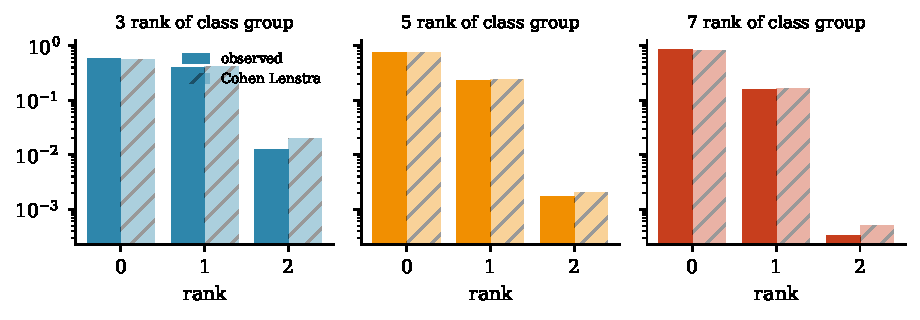
\includegraphics[width=0.92\textwidth]{figs/cohen_lenstra.pdf}
\caption{Frequencies of $3$, $5$ and $7$ ranks of class groups of imaginary quadratic fields with $10^6\le|D|\le2\cdot10^6$ (logarithmic scale), observed against the Cohen Lenstra law $p^{-r^2}\eta_\infty(p)/\prod_{k\le r}(1-p^{-k})^2$.}\label{fig:06ccohenlenstra}
\end{figure}

\begin{figure}[ht]\centering
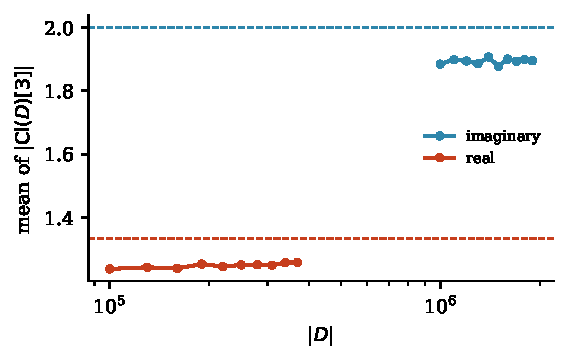
\includegraphics[width=0.7\textwidth]{figs/davenport_heilbronn.pdf}
\caption{Window means of $|\mathrm{Cl}(D)[3]|$ for imaginary ($10^6\le|D|\le2\cdot10^6$) and real ($10^5\le D\le4\cdot10^5$) quadratic fields: each range is split into ten windows with equal numbers of discriminants, and each mean is plotted at the smallest $|D|$ of its window. Dashed lines: the Davenport Heilbronn limits $2$ and $\frac43$.}\label{fig:06cdh}
\end{figure}

Three features stand out. First, the agreement improves with $p$. In the imaginary range every frequency for $p = 7$ is within $0.004$ of the prediction and every frequency for $p = 5$ within $0.006$, while for $p = 3$ the deficit in $\Prob(3\mid h)$ is $0.030$; in the real range the deficits in $\Prob(p\mid h)$ are $0.037$, $0.010$ and $0.005$ for $p = 3,5,7$. Even the small deficits are significant: in the imaginary range the binomial standard error of $\Prob(p\mid h)$ is below $0.001$, so the deficits for $p = 5$ and $p = 7$ are about $8$ and $6$ standard errors. Second, the deviations have a consistent sign: the data show too few groups with nontrivial $p$ part. Third, the mean of $|\mathrm{Cl}(D)[3]|$ is $1.8933$ in the imaginary range against the limit $2$, with window means in Figure~\ref{fig:06cdh} between $1.877$ and $1.907$ and no visible trend, and $1.2489$ in the real range against $\frac43$.

The secondary term of Theorem~\ref{thm:06csecond} accounts for the $3$ torsion deficit quantitatively. The nontrivial part of the mean, $\E|\mathrm{Cl}(D)[3]|-1$, is $0.893$ against $1$ in the imaginary range and $0.249$ against $\frac13$ in the real range, relative deficits of $0.107$ and $0.253$. Taking differences of \eqref{eq:06ctt} at the ends of our two ranges and dividing by the number of fundamental discriminants in them predicts means of $1.8933$ for $-2\cdot10^6\le D\le-10^6$ and $1.2496$ for $10^5\le D\le4\cdot10^5$, against the observed $1.8933$ and $1.2489$; with the variance of $|G[3]|$ under the Cohen Lenstra measures, the standard error of each observed mean is about $0.003$. The larger relative deficit of the real range has two sources: its discriminants are about six times smaller, which multiplies $X^{-1/6}$ by $6^{1/6} = 1.35$, and its secondary coefficient, measured against the main term of the nontrivial part ($3/\pi^2$ for $D<0$, $1/\pi^2$ for $D>0$), is larger by the factor $\sqrt3$. Across the imaginary range \eqref{eq:06ctt} predicts window means rising only from $1.887$ to $1.898$, a change comparable to the standard error $0.008$ of a single window mean, so the flat window means of Figure~\ref{fig:06cdh} are expected; across the real range it predicts a rise from $1.239$ to $1.256$, and the data go from $1.238$ to $1.259$. For $p = 5$ and $p = 7$ no secondary term is known; the smaller deficits suggest one that is smaller or decays faster. The lesson for the computational programme is that data should be compared with Cohen and Lenstra only after the secondary term is accounted for, from \eqref{eq:06ctt} where it is known and by fitting a correction $c'X^{-\theta}$ with a free exponent where it is not (Computational Problem~\ref{cp:06cclscale}).

\section{Selmer groups and the Poonen Rains model}\label{sec:06cselmer}

Let $E/\Q$ be an elliptic curve and $n\ge2$. The Kummer sequence $0\to E[n]\to E(\bar\Q)\xrightarrow{n}E(\bar\Q)\to0$ gives an injection $E(\Q)/nE(\Q)\hookrightarrow H^1(\Q,E[n])$, and similarly over every completion $\Q_v$. The $n$ Selmer group\index{Selmer group} $\operatorname{Sel}_n(E)$ is the subgroup of classes in $H^1(\Q,E[n])$ whose restriction to every $\Q_v$ lies in the image of $E(\Q_v)/nE(\Q_v)$; it is finite and effectively computable. The Shafarevich Tate group $\mathrm{Sha}(E)$\index{Shafarevich Tate group} is the group of isomorphism classes of torsors under $E$ that have a point over every completion of $\Q$, and the descent sequence reads
\begin{equation}\label{eq:06cdescent}
0\to E(\Q)/nE(\Q)\to\operatorname{Sel}_n(E)\to\mathrm{Sha}(E)[n]\to0 .
\end{equation}
When $E(\Q)[2] = 0$ we have $E(\Q)/2E(\Q)\cong(\Z/2)^{r}$, so $r(E)\le\dim_{\mathbb{F}_2}\operatorname{Sel}_2(E)$, with equality if and only if $\mathrm{Sha}(E)[2] = 0$. If $\mathrm{Sha}(E)[2^\infty]$ is finite, the Cassels Tate pairing on it is alternating and nondegenerate, so $|\mathrm{Sha}(E)[2]|$ is a square and $\dim\operatorname{Sel}_2\equiv r\pmod 2$.

\subsection{Intersections of random maximal isotropic subspaces}

Poonen and Rains \cite{poonenrains2012} proved that $\operatorname{Sel}_p(E)$ is naturally an intersection of two maximal isotropic subspaces. The restricted product $V = \prod'_vH^1(\Q_v,E[p])$, taken with respect to the unramified classes, carries a quadratic form, built from Mumford's Heisenberg group following Zarhin, whose associated bilinear form is the sum of the local Tate pairings (cup product followed by the Weil pairing). The product $Z$ of the local Kummer images, a compact open subspace, and the image $W$ of $H^1(\Q,E[p])$, a discrete one, are both maximal isotropic, and arithmetic duality gives $\operatorname{Sel}_p(E)\cong W\cap Z$. The model replaces $V$ by a finite hyperbolic quadratic space and $W,Z$ by independent uniformly random maximal isotropic subspaces.\index{Poonen Rains model}

Let $Q$ be the hyperbolic quadratic form on $V_n = \mathbb{F}_p^{2n}$ (orthogonal sum of $n$ hyperbolic planes; for odd $p$ any nondegenerate form of this discriminant). Its maximal isotropic subspaces have dimension $n$, and the following counts are classical:
\begin{enumerate}[label=(\alph*)]
\item the number of maximal isotropic subspaces of $V_n$ is $\prod_{i=0}^{n-1}(1+p^i)$;
\item for a fixed maximal isotropic $W$, the number of maximal isotropic $Z$ with $Z\cap W = 0$ is $p^{n(n-1)/2}$.
\end{enumerate}
For (b), choose a maximal isotropic $W'$ with $V_n = W\oplus W'$, so that the bilinear form identifies $W$ with the dual of $W'$; a complement of $W$ is the graph of a linear map $T:W'\to W$, and it is isotropic if and only if the bilinear form $(x,y)\mapsto\langle Tx,y\rangle$ on $W'$ is alternating (with zero diagonal, which is the quadratic condition in characteristic $2$). The alternating forms form a space of dimension $n(n-1)/2$. Statement (a) follows from (b), the decomposition by $W\cap Z$ in the proof below, and the $q$ binomial theorem.

\begin{theorem}[Poonen and Rains \cite{poonenrains2012}]\label{thm:06cpr}
Let $W,Z$ be independent uniformly random maximal isotropic subspaces of $V_n$. Then
\[
\Prob(\dim W\cap Z = d) = \binom{n}{d}_{\!p}\frac{p^{(n-d)(n-d-1)/2}}{\prod_{i=0}^{n-1}(1+p^i)},
\]
with $\binom{n}{d}_p$ the Gaussian binomial coefficient, and as $n\to\infty$
\begin{equation}\label{eq:06cprlaw}
\Prob(\dim W\cap Z = d)\to\prod_{j\ge0}(1+p^{-j})^{-1}\prod_{j=1}^d\frac{p}{p^j-1}.
\end{equation}
\end{theorem}

\begin{proof}
Fix $W$. A maximal isotropic $Z$ with $Z\cap W = U$, $\dim U = d$, is contained in $U^\perp$ and its image in $U^\perp/U$, a hyperbolic space of dimension $2(n-d)$, is maximal isotropic and meets $(W\cap U^\perp)/U = W/U$ trivially; conversely each such image lifts uniquely. By (b) there are $p^{(n-d)(n-d-1)/2}$ choices for each of the $\binom nd_p$ subspaces $U\subset W$, and dividing by (a) gives the finite formula. For the limit, write $\binom nd_p = p^{nd-d(d-1)/2}\prod_{i<d}(1-p^{i-n})/\prod_{i=1}^d(p^i-1)$ and $\prod_{i<n}(1+p^i) = p^{n(n-1)/2}\prod_{j<n}(1+p^{-j})$. The power of $p$ is $nd-\frac{d(d-1)}2+\frac{(n-d)(n-d-1)}2-\frac{n(n-1)}2 = d$, and letting $n\to\infty$ gives $p^d\prod_{j\ge0}(1+p^{-j})^{-1}/\prod_{i=1}^d(p^i-1)$, which is \eqref{eq:06cprlaw}.
\end{proof}

\begin{conjecture}[Poonen and Rains \cite{poonenrains2012}]\label{conj:06cpr}
For each prime $p$, as $E$ runs through elliptic curves over $\Q$ ordered by height, $\dim_{\mathbb{F}_p}\operatorname{Sel}_p(E)$ has the limiting distribution \eqref{eq:06cprlaw}.
\end{conjecture}

For $p = 2$ the law is $0.2097$, $0.4194$, $0.2796$, $0.0799$, $0.0107$ for $d = 0,\dots,4$, with constant $c_2 = \prod_{j\ge0}(1+2^{-j})^{-1} = 0.20971$. The model also predicts that $\dim\operatorname{Sel}_p$ is even with probability exactly $\frac12$, a point we return to in Proposition~\ref{prop:06cbernoulli}.

\subsection{The theorems of Bhargava and Shankar}

The Poonen Rains model predicts $\E|\operatorname{Sel}_p| = p+1$ (Proposition~\ref{prop:06cbernoulli}). For $p\le5$ the corresponding average over all curves has been proved, the case $p = 5$ in a preprint. Every elliptic curve over $\Q$ has a unique model $y^2 = x^3+Ax+B$ with $A,B\in\Z$ and no prime $\ell$ such that $\ell^4\mid A$ and $\ell^6\mid B$; we order curves by the naive height $H = \max(4|A|^3,27B^2)$ of this model.

\begin{theorem}[Bhargava and Shankar]\label{thm:06cbs}
Over all elliptic curves $E/\Q$ ordered by height, the average size of $\operatorname{Sel}_2(E)$ is $3$ \cite{bhargavashankar2015}, and the average size of $\operatorname{Sel}_3(E)$ is $4$ \cite{bhargavashankar2015b}. In later work, still a preprint, Bhargava and Shankar showed that the average size of $\operatorname{Sel}_5(E)$ is $6$ \cite{bhargavashankar2013}.
\end{theorem}

The method is again geometry of numbers: $2$ Selmer elements correspond to locally soluble integral binary quartic forms up to $\PGL_2(\Z)$, and $3$ Selmer elements to ternary cubic forms; the average is a ratio of volumes, and the answer $p+1$ comes out as $1$ (the identity element) plus the Tamagawa number $p$ of $\PGL_p$. Since $r\le\dim\operatorname{Sel}_p$ and $p^r\le|\operatorname{Sel}_p|$, these averages bound the average rank. Bhargava and Shankar obtain average rank at most $1.5$ from $\operatorname{Sel}_2$ and less than $1.17$ from $\operatorname{Sel}_3$; combining $\operatorname{Sel}_5$ with the $p$ parity theorem and with their proof that root numbers are equidistributed in a family of density at least $55\%$, they obtain less than $0.885$, which shows that the average rank is less than $1$.\index{average rank}

Combining the $3$ Selmer theorem with the $p$ parity theorem and with the Iwasawa main conjecture of Skinner and Urban \cite{skinnerurban2014}, Bhargava and Shankar showed that a positive proportion of elliptic curves over $\Q$ have rank $0$ and analytic rank $0$. For rank $1$ the analogous statement uses in addition the theorems of Gross and Zagier \cite{grosszagier1986} and of Kolyvagin \cite{kolyvagin1988} and the converse theorems of Skinner and of W.~Zhang, and Bhargava, Skinner and Zhang \cite{bsz2014} combined these ideas, in a preprint, to show that more than $66\%$ of elliptic curves over $\Q$ ordered by height satisfy the conjecture of Birch and Swinnerton Dyer in its rank part (analytic rank equals algebraic rank, both $0$ or $1$, with $\mathrm{Sha}$ finite). These results are unconditional, and the statements about analytic rank rest on modularity, through which $L(s,E)$ is known to be entire.

\subsection{The model of Bhargava, Kane, Lenstra, Poonen and Rains}

The Poonen Rains model concerns one prime at a time and only $\operatorname{Sel}_p$. Bhargava, Kane, Lenstra, Poonen and Rains \cite{bklpr2015} lifted it to $\Z_p$, modelling the whole sequence $0\to E(\Q)\otimes\Q_p/\Z_p\to\operatorname{Sel}_{p^\infty}(E)\to\mathrm{Sha}(E)[p^\infty]\to0$ by intersections of random maximal isotropic $\Z_p$ submodules, and showed that for curves of rank $r$ the predicted law of $\mathrm{Sha}(E)[p^\infty]$ is that of the torsion of the cokernel of a random alternating matrix over $\Z_p$ with kernel of rank $r$. In the compact form used by Park, Poonen, Voight and Wood, choose a large $n$ of uniformly random parity and a Haar random alternating matrix $A\in M_n(\Z_p)$, and put
\[
\text{rank}\leftrightarrow\operatorname{rk}_{\Z_p}\ker A,\qquad \mathrm{Sha}[p^\infty]\leftrightarrow(\operatorname{cok}A)_{\mathrm{tors}} .
\]
An alternating matrix of odd size is singular, so $\ker A$ has rank $1$ almost surely for odd $n$ and $0$ for even $n$: the model predicts rank $0$ and rank $1$ each with probability $\frac12$, rank at least $2$ with probability $0$, and $\mathrm{Sha}[p^\infty]$ finite with probability $1$. The torsion of the cokernel of an alternating matrix carries a nondegenerate alternating pairing, matching the Cassels Tate pairing, and for curves of rank $r$ the model gives $\mathrm{Sha}[p^\infty]\cong G$ with probability proportional to $|G|^{1-r}/|\operatorname{Sp}(G)|$, where $G$ runs over finite abelian $p$ groups with a nondegenerate alternating pairing and $\operatorname{Sp}(G)$ is the group of automorphisms preserving it. This symplectic analogue of Cohen and Lenstra is the distribution proposed by Delaunay \cite{delaunay2001}, in the form he later refined. The model reproduces Conjecture~\ref{conj:06cpr} for $\operatorname{Sel}_p$, and with it the averages $p+1$ of Theorem~\ref{thm:06cbs}, and it also predicts the laws of the groups $\operatorname{Sel}_{p^e}$.\index{Bhargava Kane Lenstra Poonen Rains model}

Park, Poonen, Voight and Wood \cite{ppvw2019} replaced the $p$ adic matrices by alternating integer matrices whose size $n$ and entry bound $X$ both grow with the height $H$, calibrated by $X^n = H^{1/12+o(1)}$ so that the cokernel, which models $\mathrm{Sha}$, has the size that the conjecture of Birch and Swinnerton Dyer suggests. In their model a curve of height $H$ has rank at least $r\ge1$ with probability $H^{-(r-1)/24+o(1)}$, and summing over all curves predicts that only finitely many elliptic curves over $\Q$ have rank greater than $21$, so that ranks are bounded. This is a heuristic and not a theorem; it is in tension with the long held view that ranks are unbounded, and the record curves (Elkies found one of rank at least $28$ in 2006, and Elkies and Klagsbrun one of rank at least $29$ in 2024) are compatible with it, since the heuristic allows finitely many exceptions.

\subsection{Our data}

We took the $6122$ curves $y^2 = x^3+ax+b$ with $|a|,|b|\le40$, nonzero discriminant and $x^3+ax+b$ irreducible over $\Q$, so that $E(\Q)[2] = 0$. For each we computed the root number and ran PARI/GP \texttt{ellrank}, which performs a $2$ descent, computes the $2$ part of the Cassels Tate pairing on $\operatorname{Sel}_2$ and searches for points; its output gives $\dim\operatorname{Sel}_2$ and lower and upper bounds for the rank, which coincided for all but one curve. Table~\ref{tab:06cselmer} and Figure~\ref{fig:06cselmer} summarise the $6121$ curves whose rank was determined.

\begin{table}[ht]\centering\small
\begin{tabular}{lccccc}
\toprule
 & $0$ & $1$ & $2$ & $3$ & $4$\\
\midrule
$\dim\operatorname{Sel}_2$, observed & $0.3093$ & $0.4976$ & $0.1826$ & $0.0105$ & $0$\\
$\dim\operatorname{Sel}_2$, Poonen Rains & $0.2097$ & $0.4194$ & $0.2796$ & $0.0799$ & $0.0107$\\
rank, observed & $0.3277$ & $0.4996$ & $0.1642$ & $0.0085$ & \\
\bottomrule
\end{tabular}
\caption{The $6121$ curves $y^2 = x^3+ax+b$, $|a|,|b|\le40$, with no rational $2$ torsion and rank determined by \texttt{ellrank}: distribution of $\dim\operatorname{Sel}_2$ against the Poonen Rains law, and of the rank. Mean $|\operatorname{Sel}_2| = 2.119$ (Bhargava and Shankar: $3$ in the limit); mean rank $0.853$; root number $+1$ for $49.2\%$.}\label{tab:06cselmer}
\end{table}

\begin{figure}[ht]\centering
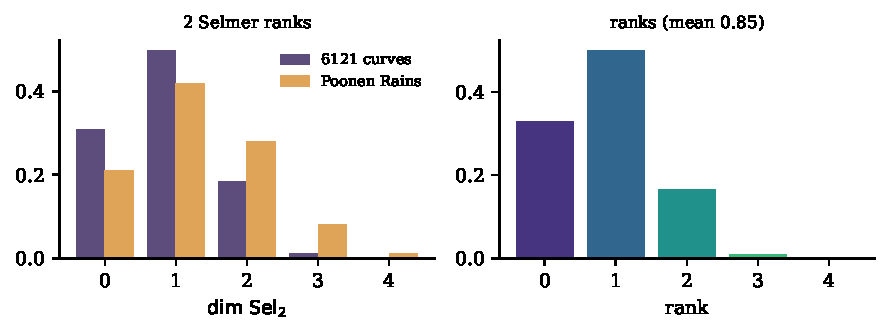
\includegraphics[width=0.92\textwidth]{figs/selmer_ranks.pdf}
\caption{Left: $\dim\operatorname{Sel}_2$ for the $6121$ curves of small height of Table~\ref{tab:06cselmer} against the Poonen Rains law. Right: their ranks (mean $0.85$).}\label{fig:06cselmer}
\end{figure}

Every frequency departs from the limiting law in the same direction: small Selmer groups are too common, and large ones too rare. The mean of $|\operatorname{Sel}_2|$ is $2.119$, not $3$. Yet the mean rank, $0.853$, is far above the conjectural limit $\frac12$, and one curve in six has rank $2$. The two effects are compatible. The mean of $\dim\operatorname{Sel}_2$ is $0.894$, only $0.041$ above the mean rank. For a curve whose rank the descent determines, $\dim\operatorname{Sel}_2-r = \dim\mathrm{Sha}(E)[2]$ is even (Section~\ref{sec:06cparity}), and here $\dim\operatorname{Sel}_2\le3$, so $\mathrm{Sha}(E)[2]\cong(\Z/2)^2$ for exactly $125$ curves ($2.0\%$) and $\mathrm{Sha}(E)[2] = 0$ for the rest: at small height, $\operatorname{Sel}_2$ is almost entirely accounted for by rational points. This is what the conjecture of Birch and Swinnerton Dyer leads one to expect, since together with standard conjectures on $L(E,1)$ it gives $|\mathrm{Sha}|$ an average size $H^{1/12+o(1)}$ over curves of rank $0$ \cite{ppvw2019}, which is small at our heights ($H\le256000$). In the model of Park, Poonen, Voight and Wood both features appear at small height: the cokernel that models $\mathrm{Sha}$ is small, and the probability of rank at least $2$ decays only like $H^{-1/24+o(1)}$. The excess of rank $2$ in small height families was documented systematically by Bektemirov, Mazur, Stein and Watkins \cite{bmsw2007}, who argued that the convergence to the limiting average is slow (a heuristic of Watkins discussed there makes the proportion of analytic rank at least $2$ among curves of root number $+1$ and discriminant near $X$ decay like $(\log X)^{3/8}X^{-1/24}$) and that the data do not contradict the minimalist conjecture. We read our table in the same cautious way: a box with $|a|,|b|\le40$ is far from the asymptotic regime. Section~\ref{sec:06cparity} examines the statistic that should already be close to its limit, the proportion of curves with root number $+1$.

\section{Ranks and $L$ functions}\label{sec:06cranks}

\subsection{Goldfeld's conjecture and the minimalist conjecture}

For a fixed $E/\Q$ of conductor $N_E$ and fundamental discriminants $d$, the quadratic twists $E_d$ have $L(s,E_d) = \sum\chi_d(n)a_nn^{-s}$ (away from the conductor), and for $d$ prime to $N_E$ the root number is $w(E_d) = \chi_d(-N_E)w(E)$, so these twists split evenly between root numbers $+1$ and $-1$.

\begin{conjecture}[Goldfeld \cite{goldfeld1979}]\label{conj:06cgoldfeld}
In the family of quadratic twists of a fixed elliptic curve over $\Q$, ordered by $|d|$, the average analytic rank is $\frac12$: asymptotically half the twists have analytic rank $0$ and half have analytic rank $1$.
\end{conjecture}

The minimalist conjecture is the analogous statement for all elliptic curves ordered by height, or for any reasonable family: the rank is as small as the root number allows, so rank $0$ when $w = +1$ and rank $1$ when $w = -1$, outside a set of density zero. Both are predictions of the Katz and Sarnak philosophy (Chapter~\ref{ch:06}): for a family with orthogonal symmetry split by root number, the zeros near the centre behave like eigenvalues near $1$ of Haar random matrices in $\mathrm{SO}(2N)$ or $\mathrm{SO}(2N+1)$, and a random matrix in $\mathrm{SO}(2N)$ has eigenvalue $1$ with probability $0$, while one in $\mathrm{SO}(2N+1)$ has it with multiplicity exactly $1$ almost surely. The random alternating matrices of the BKLPR model make the same prediction on the arithmetic side: kernel rank $0$ or $1$ according to the parity of $n$. That two random matrix models, one for zeros (orthogonal) and one for groups (alternating $p$ adic), agree on the $50/50$ split is an instance of the dictionary between the analytic and arithmetic sides of the conjecture of Birch and Swinnerton Dyer.\index{Goldfeld conjecture}\index{minimalist conjecture}

The rigorous results are bounds. Under the generalized Riemann hypothesis, the one level density methods of Brumer, Heath Brown and Young described in Section~\ref{sec:ch6ils} bound the average analytic rank; the Bhargava and Shankar theorems give unconditional bounds for the average algebraic rank. In quadratic twist families Smith \cite{smith2017} proved, in a preprint, that for $E/\Q$ with full rational $2$ torsion and no rational cyclic subgroup of order $4$ the $2^\infty$ Selmer groups of the twists $E_d$ have the distribution predicted by Delaunay's heuristic, and deduced that the twists of rank at least $2$ have density zero, the algebraic heart of Goldfeld's conjecture for these families.

\subsection{Root numbers and parity}\label{sec:06cparity}

Among the $6121$ curves of Table~\ref{tab:06cselmer} the root number is $+1$ for $49.2\%$, and for every one of them the rank is even exactly when $w(E) = +1$. This is what the parity conjecture $(-1)^{r(E)} = w(E)$ predicts; it follows from the conjecture of Birch and Swinnerton Dyer and is open in general. What is proved is the $p$ parity conjecture: Monsky \cite{monsky1996} showed that $(-1)^{\dim\operatorname{Sel}_2(E)-\dim E(\Q)[2]} = w(E)$ for every $E/\Q$, and T.~and V.~Dokchitser \cite{dokchitser2010} proved that the $\Z_p$ corank of the $p^\infty$ Selmer group has the parity of the root number for every $E/\Q$ and every prime $p$. Rank parity follows for every curve with $\mathrm{Sha}(E)[p^\infty]$ finite for one $p$, since that corank is then the rank. Our check is therefore not independent evidence for the parity conjecture. The upper bound that \texttt{ellrank} computes exceeds the rank by the dimension of $2\,\mathrm{Sha}(E)[4]$, so when the bounds coincide $\mathrm{Sha}(E)$ has no element of order $4$; then $\mathrm{Sha}(E)[2^\infty] = \mathrm{Sha}(E)[2]$ is finite, of even dimension, and Monsky's theorem forces the agreement. For the same reason the even parts of the two distributions, $0.3093+0.1826$ and $0.3277+0.1642$, both equal the root number proportion $0.4919$. What the data test is the equidistribution of root numbers, and $0.4919$ is within $1.3$ standard errors of $\frac12$.

\subsection{The rank as a Thorin atom and as a bias}

The rank enters the analytic theory of this book in two further guises. In Chapter~\ref{ch:05} we saw that the partial sums $\sum_{p\le x}a_p\log p/p$ drift like $(\frac12-r)\log x$ in logarithmic mean under the Riemann hypothesis for $L(s,E)$ (Section~\ref{sec:05bias}, Table~\ref{tab:05bias}): the central zero of order $r$ appears, through the explicit formula, as a bias in Frobenius traces. In Chapter~\ref{ch:10b} (Proposition~\ref{prop:10brank}) the same central zero appears as a degenerate Thorin atom: $\log|\Lambda(\frac12+\sqrt s,E)|$ has slope $r/2$ in $\log s$ near $s = 0$, a gamma factor of shape $r/2$ whose Thorin mass has escaped to the origin. In the language of the present chapter the minimalist conjecture, in its analytic form, says that in a family this atom has mass $0$ or $\frac12$ according to the root number, each with probability $\frac12$, and that the larger masses $1,\frac32,\dots$ occur with density zero. Our small height data, with mean rank $0.853$, put visible weight on the larger masses: by the theorems of Gross and Zagier \cite{grosszagier1986} and Kolyvagin \cite{kolyvagin1988} a curve of rank at least $2$ has analytic rank at least $2$, and $17.3\%$ of our curves have rank at least $2$. The rank bias and the Thorin atom read the order of vanishing at the centre directly; the Selmer statistics read it through the conjecture of Birch and Swinnerton Dyer.

\subsection{The Poonen Rains law as a sum of independent coins}

We close the mathematical part of the chapter with a structural description of the Poonen Rains law that makes its moments transparent.

\begin{proposition}[Poonen and Rains \cite{poonenrains2012}]\label{prop:06cbernoulli}
Let $\xi_0,\xi_1,\dots$ be independent with $\Prob(\xi_i = 1) = 1/(1+p^i) = 1-\Prob(\xi_i = 0)$. Then:
\begin{enumerate}[label=(\alph*)]
\item for each $n$, $\dim W\cap Z$ in Theorem~\ref{thm:06cpr} has the law of $\xi_0+\dots+\xi_{n-1}$, and the Poonen Rains law \eqref{eq:06cprlaw} is the law of $S = \sum_{i\ge0}\xi_i$, which is almost surely finite;
\item $\E t^S = \prod_{i\ge0}(t+p^i)/(1+p^i)$ for all complex $t$;
\item $\Prob(S\text{ even}) = \frac12$, and $S$ is even with probability $\frac12$ conditionally on $\xi_1,\xi_2,\dots$;
\item $\E p^S = p+1$, and more generally $\E\prod_{j=0}^{k-1}(p^S-p^j) = p^{k(k+1)/2}$ for $k\ge1$;
\item $\E S = \sum_{i\ge0}(1+p^i)^{-1}$ and $\operatorname{Var}S = \sum_{i\ge0}p^i(1+p^i)^{-2}$; for $p = 2$ these are $1.2645$ and $0.8463$;
\item $\Prob(S = 0) = c_p := \prod_{j\ge0}(1+p^{-j})^{-1}$ and $\Prob(S\ge2) = 1-\frac{2p-1}{p-1}\,c_p$, equal to $1-3c_2 = 0.3709$ for $p = 2$.
\end{enumerate}
\end{proposition}

\begin{proof}
(a) By Theorem~\ref{thm:06cpr} the generating function of $\dim W\cap Z$ is
\[
\begin{aligned}
\E t^{\dim W\cap Z} &= \frac{1}{\prod_{i<n}(1+p^i)}\sum_{d=0}^n\binom nd_{\!p}p^{(n-d)(n-d-1)/2}t^d\\
&= \frac{t^n}{\prod_{i<n}(1+p^i)}\sum_{e=0}^n\binom ne_{\!p}p^{e(e-1)/2}t^{-e},
\end{aligned}
\]
substituting $e = n-d$ and using $\binom nd_p = \binom n{n-d}_p$. The $q$ binomial theorem $\sum_e\binom ne_pp^{e(e-1)/2}u^e = \prod_{i<n}(1+p^iu)$ with $u = 1/t$ gives $\prod_{i<n}(t+p^i)/(1+p^i)$, the generating function of $\xi_0+\dots+\xi_{n-1}$, since $(t+p^i)/(1+p^i) = \Prob(\xi_i = 0)+t\Prob(\xi_i = 1)$. Since $\sum_i\Prob(\xi_i = 1)<\infty$, Borel and Cantelli show that only finitely many $\xi_i$ equal $1$, so the partial sums converge almost surely to $S<\infty$; hence the laws converge pointwise, and the limit is \eqref{eq:06cprlaw} by Theorem~\ref{thm:06cpr}. (b) The partial products converge for every $t$ because $\sum_i|t-1|/(1+p^i)<\infty$, and $\E t^{S_n}\to\E t^S$ by dominated convergence for $|t|\le1$ and, for larger $|t|$, by the bound $|t|^{S_n}\le|t|^S$ and the finiteness of $\E|t|^S = \prod_i(|t|+p^i)/(1+p^i)$ (monotone convergence). (c) $\xi_0$ is a fair coin independent of $\xi_1,\xi_2,\dots$, so the parity of $S$ is a fair coin given the rest. (d) Fix $W$ in $V_n$ and $k\le n$. A $k$ tuple of linearly independent vectors in $W\cap Z$ spans a $k$ dimensional subspace $U\subset W$, and, as in the proof of Theorem~\ref{thm:06cpr}, the maximal isotropic $Z$ containing a given $U$ correspond to the maximal isotropic subspaces of $U^\perp/U\cong V_{n-k}$, of which there are $\prod_{i<n-k}(1+p^i)$. Counting pairs,
\[
\E\prod_{j<k}\bigl(p^{\dim W\cap Z}-p^j\bigr) = \prod_{j<k}(p^n-p^j)\,\frac{\prod_{i<n-k}(1+p^i)}{\prod_{i<n}(1+p^i)} = \prod_{j<k}\frac{p^n-p^j}{1+p^{n-k+j}} ,
\]
which tends to $\prod_{j<k}p^{k-j} = p^{k(k+1)/2}$ as $n\to\infty$. By (a) the left side is $\E f(S_n)$ with $S_n = \xi_0+\dots+\xi_{n-1}$ and $f(m) = \prod_{j<k}(p^m-p^j)$, which is nonnegative and nondecreasing on the integers; since $S_n$ increases to $S$, monotone convergence gives $\E f(S) = p^{k(k+1)/2}$. The case $k = 1$ is $\E p^S = p+1$. (e) Sum the Bernoulli means and variances. (f) $\Prob(S = 0) = \prod_i\Prob(\xi_i = 0) = \prod_ip^i/(1+p^i)$, and $\Prob(S = 1) = \Prob(S = 0)\sum_i\Prob(\xi_i = 1)/\Prob(\xi_i = 0) = \Prob(S = 0)\sum_ip^{-i} = \Prob(S = 0)\,p/(p-1)$.
\end{proof}

Parts (a) and (b) are Proposition~2.6 of Poonen and Rains, (c) is their Proposition~2.22(b), and (d) is equivalent to their Proposition~2.22(a); in the form stated, (d) is the prime case of a theorem of Bhargava, Kane, Lenstra, Poonen and Rains \cite{bklpr2015}, proved there by the same count. The independent coin form separates parity from size. For a curve with $E(\Q)[p] = 0$ the theorem of Dokchitser and Dokchitser gives $(-1)^{\dim\operatorname{Sel}_p(E)} = w(E)$, because $\operatorname{Sel}_p(E) = \operatorname{Sel}_{p^\infty}(E)[p]$ and the quotient of $\operatorname{Sel}_{p^\infty}(E)$ by its divisible part, which carries the nondegenerate alternating Cassels Tate pairing, has $p$ torsion of even dimension. In the model the parity of $S$ plays the role of $w(E)$, and by (c) it is a fair coin even given $\xi_1,\xi_2,\dots$, as equidistributed root numbers require. In the BKLPR model the rank $r$ is $0$ or $1$ almost surely and $\dim\operatorname{Sel}_p = r+\dim\mathrm{Sha}[p]$ with $\dim\mathrm{Sha}[p]$ even, so $r$ is the parity of $S$ and $\dim\mathrm{Sha}[p] = 2\lfloor S/2\rfloor$; for $p = 2$ the coins $\xi_1,\xi_2,\dots$, with probabilities $\frac13,\frac15,\frac19,\dots$, govern its size.

\begin{corollary}[Rank bounds from the model]\label{cor:06cbound}
Consider a family of elliptic curves over $\Q$ with $E(\Q)[2] = 0$, ordered by a height, in which $\dim\operatorname{Sel}_2(E)$ converges in distribution to the Poonen Rains law \eqref{eq:06cprlaw} for $p = 2$ and the average of $|\operatorname{Sel}_2(E)|$ over the curves of height at most $X$ stays bounded as $X\to\infty$. Then the average rank $\bar r(X)$ of the curves of height at most $X$ satisfies
\[
\limsup_{X\to\infty}\bar r(X)\le\E S = \sum_{i\ge0}\frac{1}{1+2^i} = 1.2645 < \log_2\E2^S = \log_23 = 1.585 ,
\]
where $S$ has the law \eqref{eq:06cprlaw} for $p = 2$.
\end{corollary}

\begin{proof}
Since $E(\Q)[2] = 0$, the Kummer map embeds $E(\Q)/2E(\Q)\cong(\Z/2)^r$ in $\operatorname{Sel}_2(E)$, so $r\le\dim\operatorname{Sel}_2(E)$. For every $\varepsilon>0$ there is $C_\varepsilon$ with $m\le C_\varepsilon+\varepsilon2^m$ for all $m\ge0$, so bounded averages of $2^{\dim\operatorname{Sel}_2}$ make $\dim\operatorname{Sel}_2$ uniformly integrable along the family, and its averages converge to $\E S$, which Proposition~\ref{prop:06cbernoulli}(e) evaluates. The last comparison is Jensen's inequality for the concave logarithm, strict because $S$ is not constant, with $\E2^S = 3$ from Proposition~\ref{prop:06cbernoulli}(d).
\end{proof}

The comparison clarifies what an average of $|\operatorname{Sel}_2|$ alone can give. Knowing only that the average of $|\operatorname{Sel}_2|$ is $3$, as Bhargava and Shankar proved, Jensen yields average rank at most $\log_23\approx1.585$; the integer inequality $2r\le2^r$ does better and yields their bound $1.5$. Knowing in addition the full Poonen Rains law would give $1.2645$. The same argument with the integer inequalities $r\le\frac12+\frac16\,3^r$ and $r\le\frac34+\frac1{20}\,5^r$, both equalities at $r = 1,2$, turns the $3$ Selmer average $4$ into their bound $\frac76\approx1.17$ and the $5$ Selmer average $6$ into $1.05$, before the parity input described after Theorem~\ref{thm:06cbs}. The value $\frac12$ is out of reach of the Selmer group at any single prime, even with its full law: Selmer data alone cannot exclude $r = \dim\operatorname{Sel}_p$, so the best bound they give is $\E\dim\operatorname{Sel}_p = \sum_{i\ge0}(1+p^i)^{-1}$ in the model, which exceeds $\frac12$ for every $p$. It tends to $\frac12$ as $p\to\infty$, and Rubin observed \cite{poonenrains2012} that the law \eqref{eq:06cprlaw} itself tends to the fair coin on $\{0,1\}$. Hence the average rank would be at most $\frac12$ if Conjecture~\ref{conj:06cpr} and the average $p+1$ of $|\operatorname{Sel}_p|$, which Poonen and Rains also conjecture, held for infinitely many $p$. The law alone for infinitely many $p$ would give the density statements that almost all curves have rank at most $1$ and at least half have rank $0$, but not the bound on the average, since a set of curves of density zero and large rank could raise it.

\section{Notes}

Cohen and Lenstra \cite{cohenlenstra1984} introduced the heuristics in the Noordwijkerhout proceedings, with extensive tables; Cohen and Martinet \cite{cohenmartinet1990} extended them to general number fields. The random matrix interpretation is due to Friedman and Washington \cite{friedmanwashington1989}, in the function field setting, where the $\ell$ part of the class group is the cokernel of $1-\Frob$ acting on the $\ell$ adic Tate module of the Jacobian. Hall's identity \cite{hall1938} predates both. Wood developed the moment method \cite{wood2017} and showed \cite{wood2019} that cokernels of random integral matrices with quite general independent entries have Cohen Lenstra limits, a universality phenomenon analogous to the universality of eigenvalue statistics in Chapter~\ref{ch:06}. The sandpile groups of supersingular isogeny graphs, which are modules over a Hecke algebra $\mathbb T$, behave differently: for a fixed characteristic $N\equiv1\bmod12$, growing isogeny degree and all but finitely many primes $r$, their $r$ parts follow the law of $\mathbb T_r/\det(\gamma-1)\mathbb T_r$ for $\gamma$ Haar random in the subgroup of $\GL_2(\mathbb T_r)$ with determinant in $\Z_r^\times$, where $\mathbb T_r=\mathbb T\otimes\Z_r$, and this law is not the Cohen Lenstra law (Munier and Shnidman \cite{muniershnidman2023}; Chapter~\ref{ch:hit}).

The theorem of Davenport and Heilbronn \cite{davenportheilbronn1971} is still the only determination of the mean of $|\mathrm{Cl}(D)[p]|$ over quadratic fields for an odd prime $p$. Bhargava's higher composition laws and his count of quartic rings and fields \cite{bhargava2005} carried such averages beyond the quadratic case; the secondary term \cite{bst2013,taniguchithorne2013} confirmed Roberts's conjecture. The function field results \cite{evw2016} brought topology (homological stability of Hurwitz spaces) into arithmetic statistics. The corrections at roots of unity are in Malle \cite{malle2008}.

The Poonen Rains model \cite{poonenrains2012} was motivated in part by the earlier theorems of Heath Brown on $2$ Selmer groups in the congruent number family and of Swinnerton Dyer and Kane on quadratic twists of curves with full rational $2$ torsion and no rational cyclic subgroup of order $4$, which give the law \eqref{eq:06cprlaw} for $p = 2$, shifted by $2$ to account for $E[2]$, in these twist families. The theorems of Bhargava and Shankar \cite{bhargavashankar2015,bhargavashankar2015b,bhargavashankar2013} and the synthesis of \cite{bklpr2015} and \cite{ppvw2019} now frame the subject, and the database of Balakrishnan, Ho, Kaplan, Spicer, Stein and Weigandt \cite{bhkssw2016} tests these models on hundreds of millions of curves ordered by height. Bektemirov, Mazur, Stein and Watkins \cite{bmsw2007} discuss the tension between data and the minimalist conjecture. The proposal that the Langlands programme be read alongside random group models is not ours; it is implicit in the way the conjecture of Birch and Swinnerton Dyer connects automorphic $L$ functions to Selmer and Shafarevich Tate groups.

\section{Exercises}

\begin{enumerate}
\item (Hall's identity in small order.) List the abelian groups of order $p^2$ and $p^3$ with their automorphism groups, and verify that $\sum_{|G| = p^n}|\operatorname{Aut}G|^{-1}$ equals the coefficient of $x^n$ in $\prod_{k\ge1}(1-xp^{-k})^{-1}$ for $n = 1,2,3$. Deduce \eqref{eq:06chall} by setting $x = 1$, assuming the generating function identity.
\item (Rank $0$ over a finite field.) Show that the probability that a uniformly random $n\times n$ matrix over $\mathbb{F}_p$ is invertible is $\eta_n(p)$, that it decreases in $n$, and that $0\le\eta_n(p)-\eta_\infty(p)\le p^{-n}/(p-1)$. Compute $\eta_n(2)$ for $n = 1,\dots,5$ and compare with $\eta_\infty(2) = 0.2888$.
\item (Poonen Rains at $d = 0$.) Using Theorem~\ref{thm:06cpr}, show that $\Prob(\operatorname{Sel}_2 = 0)$ is predicted to be $\prod_{j\ge0}(1+2^{-j})^{-1} = 0.2097$, and that the finite $n$ value is $2^{n(n-1)/2}/\prod_{i<n}(1+2^i)$. Compute it for $n = 1,\dots,6$.
\item (The constant at $3$.) Compute $\eta_\infty(3)$ to six digits using Euler's pentagonal number theorem, $\eta_\infty(p) = \sum_{k\in\Z}(-1)^kp^{-k(3k-1)/2}$, and determine how many terms are needed for six digits. Deduce the Cohen Lenstra prediction $\Prob(3\mid h(D)) = 0.4399$.
\item (Mean of $|G[p]|$.) Let $\bar A$ be a uniformly random $n\times n$ or $n\times(n+1)$ matrix over $\mathbb{F}_p$. By summing $\Prob(\bar A^{\mathsf T}v = 0)$ over $v\in\mathbb{F}_p^n$, show that $\E|\ker\bar A^{\mathsf T}|$ equals $2-p^{-n}$ in the square case and $1+p^{-1}-p^{-n-1}$ in the rectangular case. Since $|G[p]| = p^{\operatorname{rk}_pG}$ and $p^{\operatorname{rk}_p\operatorname{cok}A} = |\ker\bar A^{\mathsf T}|$ when $\bar A$ is the reduction of $A$ modulo $p$, deduce $\E_{\mu_{\mathrm{CL}}}|G[p]| = 2$ and $\E_{\mu^+_{\mathrm{CL}}}|G[p]| = 1+p^{-1}$, justifying the passage to the limit as in the proof of Proposition~\ref{prop:06cmoments}. Compare with Theorem~\ref{thm:06cdh}.
\item (Parity.) In the setting of Proposition~\ref{prop:06cbernoulli}, show that $\E(-1)^S = 0$, by evaluating the generating function at $t = -1$, and that $\Prob(\dim W\cap Z\text{ even}) = \frac12$ for every finite $n\ge1$. Show that if root numbers in a family of curves without rational $2$ torsion are $+1$ and $-1$ with limiting proportions $\frac12(1+\beta)$ and $\frac12(1-\beta)$, then by Monsky's theorem $\dim\operatorname{Sel}_2$ cannot follow the Poonen Rains law unless $\beta = 0$. Check that our data, with $\beta = -0.016$, are consistent with $\beta = 0$ at the usual significance levels.
\end{enumerate}

\section{Open computational problems}

\begin{compproblem}[Cohen Lenstra at scale with the secondary term]\label{cp:06cclscale}
Objective: measure the convergence of $3$, $5$ and $7$ parts of class groups of quadratic fields to the Cohen Lenstra laws, separating the secondary term. Objects: fundamental discriminants $D$, imaginary and real, all those with $|D|\le10^9$ and all those in the windows $X-10^8<|D|\le X$ for $X = 10^{10}$ and $10^{11}$. Route: PARI/GP \texttt{quadclassunit} (conditional on the generalized Riemann hypothesis, as for our data) or the subexponential class group algorithms of Jacobson and collaborators, distributed over discriminant windows on a cluster; for $3$ torsion alone, count cubic fields with Belabas's program as an unconditional check. Deliverable: tables of $p$ rank frequencies and of the means of $|\mathrm{Cl}(D)[p]|$ per window; a weighted least squares fit of $c+c'X^{-1/6}+c''X^{-1/3}$ to the $3$ torsion means, with the fitted $c'$ compared with the constants of Bhargava, Shankar and Tsimerman and of Taniguchi and Thorne; analogous fits for $p = 5,7$ with a free exponent. Why it matters: Table~\ref{tab:06cprank} shows a $3$ deficit of the size of the secondary term; a free exponent fit for $p\ge5$ would give an empirical rate of convergence where no theorem is known.
\end{compproblem}

\begin{compproblem}[Selmer groups and ranks by height]\label{cp:06cheight}
Objective: test the Poonen Rains law and the boundedness heuristic of Park, Poonen, Voight and Wood on curves ordered by height. Objects: all curves $y^2 = x^3+Ax+B$ with naive height $H\le10^{10}$ (about $10^8$ curves), with the database of Balakrishnan, Ho, Kaplan, Spicer, Stein and Weigandt \cite{bhkssw2016} as a starting point. Route: $2$ descent by PARI/GP \texttt{ellrank} or Magma, $3$ Selmer groups by Magma where feasible, root numbers from local data, and analytic ranks by \texttt{lfun} for a random subsample, distributed over curves on a cluster. Deliverable: the distribution of $\dim\operatorname{Sel}_2$ and $\dim\operatorname{Sel}_3$ in height windows, the mean of $|\operatorname{Sel}_2|$ against $3$, the proportion of rank $\ge2$ as a function of $H$ with a fitted power law, and the tail counts of rank $\ge r$ against the exponents predicted by \cite{ppvw2019}. Why it matters: the excess of curves of rank at least $2$ in Table~\ref{tab:06cselmer} must decay if the minimalist conjecture holds, and its rate of decay is what separates slow convergence from a genuine bias.
\end{compproblem}

\begin{compproblem}[Shafarevich Tate groups against BKLPR]
Objective: compare the analytic orders of $\mathrm{Sha}$ with the alternating cokernel model of \cite{bklpr2015} and with Delaunay's distribution. Objects: all curves of conductor up to $5\cdot10^5$ in Cremona's tables and the LMFDB \cite{lmfdb}, plus quadratic twist families of $11a1$ and $37a1$ with $|d|\le10^7$. Route: the analytic order of $\mathrm{Sha}$ from the leading term of $L(s,E)$ via the conjecture of Birch and Swinnerton Dyer (PARI/GP \texttt{ellbsd} and \texttt{lfun}), checked against $2$, $3$ and $4$ descents in Magma. Deliverable: the empirical law of $\mathrm{Sha}[p^\infty]$ for $p = 2,3,5$ in conductor windows, the proportion of nontrivial $\mathrm{Sha}$ as a function of conductor, and a fit of the effective matrix size in the model of Park, Poonen, Voight and Wood as a function of the conductor. Why it matters: our data show $\mathrm{Sha}[2]$ nontrivial for only $2\%$ of small curves; tracking how this grows tests the calibration on which the boundedness heuristic rests.
\end{compproblem}

\begin{compproblem}[Class groups of cubic and quartic fields]
Objective: test the Cohen Martinet heuristics, with Malle's corrections at roots of unity, for class groups of cubic and quartic fields. Objects: all cubic fields with $|D|\le10^{9}$ (enumerated by Belabas's algorithm) and all quartic fields with $|D|\le10^{8}$ with Galois groups $D_4$, $A_4$, $S_4$ and $C_4$; class groups for primes $p\le7$, with separate treatment of fields containing $\mu_p$ or with Galois closure containing it. Route: PARI/GP \texttt{bnfinit} under GRH, with spot certification by \texttt{bnfcertify}; Bhargava's parametrisations to enumerate quartic fields. Deliverable: $p$ rank frequencies against Cohen Martinet, including the average of $|\mathrm{Cl}[2]|$ for cubic fields against Bhargava's $\frac54$ and $\frac32$, and a table of the discrepancies at roots of unity against Malle's proposed corrections. Why it matters: these are the class groups attached to $\GL_1$ over fields of degree $3$ and $4$, and the cases where the heuristics are known to need correction are precisely where the arithmetic constraints are subtle.
\end{compproblem}

\part{Random Walks and Hitting Times}
\chapter{Hecke Operators as Random Walks on Trees}\label{ch:07}

In 1959 Harry Kesten computed the probability that a symmetric random walk on a free group returns to its starting point, and found that it decays exponentially, like $\rho^n$ with $\rho<1$ up to a polynomial factor \cite{kesten1959}. The work of Ihara on discrete subgroups of $\PGL_2(\Q_q)$ and Serre's lectures on trees \cite{ihara1966,serre1980} identified the regular tree on which such a walk lives with the Bruhat Tits tree of $\PGL_2(\Q_q)$, on which the Hecke operator $T_q$ of the theory of modular forms acts as the adjacency operator. In 1981 McKay found Kesten's spectral law again as the limiting eigenvalue distribution of large random regular graphs \cite{mckay1981}, and in 1997 Serre found it once more as the limiting distribution of the eigenvalues of $T_q$ on spaces of modular forms of growing level or weight \cite{serre1997}. This chapter explains why these are one law. We prove the tree theorem (Theorem~\ref{thm:07tree}), state the vertical Sato Tate theorem with a probabilistic proof idea, and test it on supersingular isogeny graphs at $207$ prime levels.

\section{The Bruhat Tits tree}\index{Bruhat Tits tree}

Fix a prime $q$. A lattice in $\Q_q^2$ is a $\Z_q$ submodule $\Z_qu\oplus\Z_qv$ spanned by a basis $u,v$ of $\Q_q^2$, and two lattices $L,L'$ are homothetic if $L'=cL$ for some $c\in\Q_q^\times$. The vertices of $\T_q$ are homothety classes $[L]$. Two classes are joined by an edge if they have representatives with $qL\subsetneq L'\subsetneq L$. Since $L/qL\cong\mathbb{F}_q^2$ has exactly $q+1$ lines, every vertex has $q+1$ neighbours, and one shows that the resulting graph is connected and has no cycles, so $\T_q$ is the $(q+1)$ regular tree \cite{serre1980}. The group $\GL_2(\Q_q)$ acts on lattices, the centre acts trivially on classes, and $\PGL_2(\Q_q)$ acts on $\T_q$ by automorphisms, transitively on vertices, with the stabiliser of $[\Z_q^2]$ equal to $\PGL_2(\Z_q)=\GL_2(\Z_q)/\Z_q^\times$, a maximal compact subgroup. Thus the vertex set is $\PGL_2(\Q_q)/\PGL_2(\Z_q)$, and functions on vertices are right $\PGL_2(\Z_q)$ invariant functions on the group.

If $L'\subseteq L$ and $L/L'\cong\Z/q^a\oplus\Z/q^b$ with $a\ge b$, then $d([L],[L'])=a-b$. For $n\ge1$ the sphere $\{w:d(v,w)=n\}$ around a vertex $v$ has $(q+1)q^{n-1}$ elements.

\subsection{Hecke operators}\index{Hecke operator}

The Hecke operator $T_q$ acts on functions on lattice classes by $T_qf([L])=\sum f([L'])$, summed over the $q+1$ sublattices of index $q$. This is the adjacency operator $A$ of $\T_q$. More generally let $A_n$ be the operator $A_nf(v)=\sum_{d(v,w)=n}f(w)$, with $A_0=I$; equivalently $A_n(v,w)$ counts nonbacktracking walks of length $n$ from $v$ to $w$, since on a tree such a walk is a geodesic and there is exactly one between vertices at distance $n$.\index{nonbacktracking operator} The classical Hecke operator $T_{q^n}$ sums over all sublattices of index $q^n$; each of them is $q^bL''$ with $L/L''$ cyclic of order $q^{n-2b}$, so on classes $T_{q^n}=A_n+A_{n-2}+A_{n-4}+\cdots$ (Exercise~\ref{ex:07hecke}). All these operators commute: they lie in the spherical Hecke algebra, which is the polynomial algebra $\C[T_q]$.

\section{The tree theorem}

Let $o$ be a fixed vertex and let $\mu_q$ be the spectral measure of the bounded self adjoint operator $X=q^{-1/2}A$ on $\ell^2(\T_q)$ at $\delta_o$, so that $\langle\delta_o,\phi(X)\delta_o\rangle=\int\phi\,d\mu_q$ for continuous $\phi$. Write $U_n$ for the Chebyshev polynomials of the second kind, $U_n(\cos\theta)=\sin((n+1)\theta)/\sin\theta$, and recall from Chapter~\ref{ch:04} that the $U_n(x/2)$ are orthonormal for the Sato Tate measure $\ST(dx)=\sqrt{4-x^2}\,dx/(2\pi)$ on $[-2,2]$.

\begin{theorem}[Tree theorem, this book]\label{thm:07tree}\index{Kesten McKay law}
Let $q\ge2$ be an integer, let $\T_q$ be the $(q+1)$ regular tree, and put $B_n=q^{-n/2}A_n$.
\begin{enumerate}
\item $B_1=U_1(X/2)$ and $B_n=U_n(X/2)-q^{-1}U_{n-2}(X/2)$ for $n\ge2$.
\item $c_n=\int U_n(x/2)\,d\mu_q(x)$ equals $q^{-n/2}$ for $n$ even and $0$ for $n$ odd.
\item $\mu_q$ is supported on $[-2,2]$ with the Kesten McKay density
\[
\mu_q(dx)=\frac{q+1}{(q^{1/2}+q^{-1/2})^2-x^2}\cdot\frac{\sqrt{4-x^2}}{2\pi}\,dx .
\]
\item If $S$ is simple random walk on $\T_q$ started at $o$, then for $m\ge0$
\[
\int x^{2m}\,d\mu_q=(q+1)^{2m}q^{-m}\Prob(S_{2m}=o).
\]
\item The walk returns to $o$ with probability $1/q$, and the Green function $G(1)=\sum_{n\ge0}\Prob(S_n=o)$, the expected number of visits to $o$, equals $q/(q-1)$.\index{Green function}
\item $\mu_q\Rightarrow\ST$ weakly as $q\to\infty$.
\end{enumerate}
\end{theorem}

\begin{proof}
(1) A vertex at distance $n\ge1$ from $w$ has one neighbour at distance $n-1$ and $q$ neighbours at distance $n+1$, while $w$ itself has $q+1$ neighbours at distance $1$. For $n\ge1$ the entry $(AA_n)(v,w)$ counts the neighbours of $v$ at distance $n$ from $w$, so it is $1$ if $d(v,w)=n+1$, $q$ if $d(v,w)=n-1\ge1$, $q+1$ if $n=1$ and $v=w$, and $0$ otherwise. Hence
\[
AA_1=A_2+(q+1)I,\qquad AA_n=A_{n+1}+qA_{n-1}\quad(n\ge2).
\]
Dividing by $q^{(n+1)/2}$, $XB_1=B_2+(1+q^{-1})I$ and $XB_n=B_{n+1}+B_{n-1}$ for $n\ge2$. The Chebyshev recursion $xU_n(x/2)=U_{n+1}(x/2)+U_{n-1}(x/2)$, with $U_0=1$ and $U_1(x/2)=x$, gives $B_1=X=U_1(X/2)$ and
\[
B_2=XU_1(X/2)-(1+q^{-1})I=U_2(X/2)-q^{-1}U_0(X/2).
\]
For $n\ge2$ the recursion $B_{n+1}=XB_n-B_{n-1}$ is linear and is satisfied separately by the sequences $U_n(X/2)$ and $q^{-1}U_{n-2}(X/2)$; since the formula holds for $n=2$ and, with the convention $U_{-1}=0$, also for $n=1$, induction proves (1).

(2) The tree has no cycles, so a nonbacktracking walk of positive length never returns: $\langle\delta_o,B_n\delta_o\rangle=0$ for $n\ge1$. Taking the $(o,o)$ entry of (1) gives $c_1=0$ and $c_n=q^{-1}c_{n-2}$ for $n\ge2$, and $c_0=1$. Hence $c_{2m}=q^{-m}$ and $c_{2m+1}=0$.

(3) Put $R=(q+1)/\sqrt q$, so that $\mu_q$ lives on $[-R,R]$ because $\|X\|\le R$. Since $\sum_nc_n^2<\infty$, the series $f=\sum_nc_nU_n(x/2)$ converges in $L^2(\ST)$. With $x=2\cos\theta$ and $U_{2m}(\cos\theta)=\sum_{|j|\le m}e^{2ij\theta}$, summing over $m\ge|j|$ first (the double series converges absolutely),
\[
\begin{aligned}
f&=\sum_{m\ge0}q^{-m}\sum_{|j|\le m}e^{2ij\theta}=\frac{q}{q-1}\sum_{j\in\Z}q^{-|j|}e^{2ij\theta}\\
&=\frac{q+1}{q}\cdot\frac{1}{1-2q^{-1}\cos2\theta+q^{-2}},
\end{aligned}
\]
a Poisson kernel. Since $2\cos2\theta=x^2-2$, the denominator equals $q^{-1}\bigl((q^{1/2}+q^{-1/2})^2-x^2\bigr)$, which gives the stated density, positive and bounded on $[-2,2]$. The measure $f\,d\ST$ has Chebyshev moments $c_n$ by orthonormality, hence the same moments $\int x^k$ as $\mu_q$, because the $U_n(x/2)$ span the polynomials. Both laws live on $[-R,R]$, so they coincide by Theorem~\ref{thm:A:moments}. In particular $\mu_q$ is supported on $[-2,2]$.

(4) By definition $\int x^{2m}\,d\mu_q=q^{-m}A^{2m}(o,o)$, and $A^{2m}(o,o)$ is the number of closed walks of length $2m$ at $o$, each of which simple random walk follows with probability $(q+1)^{-2m}$.

(5) Let $D_n=d(o,S_n)$. By the neighbour count in (1), $D$ is a Markov chain on $\{0,1,2,\dots\}$: from $0$ it moves to $1$, and from $k\ge1$ it moves up with probability $q/(q+1)$ and down with probability $1/(q+1)$. By the gambler's ruin formula for a walk with upward drift, the probability of ever reaching $0$ from $1$ is $(1/(q+1))/(q/(q+1))=1/q$. Since the first step from $o$ goes to distance one, the return probability is $1/q$, the number of visits to $o$ (counting time $0$) is geometric with mean $1/(1-1/q)$, and $G(1)=q/(q-1)$.

(6) For each $n\ge1$, $c_n\to0=\int U_n(x/2)\,d\ST$ as $q\to\infty$. All measures live on $[-2,2]$, where polynomials are dense in the continuous functions, so $\int\phi\,d\mu_q\to\int\phi\,d\ST$ for every continuous $\phi$.
\end{proof}

The density of $\mu_q$ relative to $\ST$ is $q/(q-1)$ times the Poisson kernel with parameter $q^{-1}$ at the angle $2\theta$. It increases with $|x|$, so $\mu_q$ puts more mass near $\pm2$ than the semicircle does, and it tends to $1$ uniformly on $[-2,2]$ as $q\to\infty$ (Figure~\ref{fig:07kestenmckay}). Since $\Prob(S_n=o)=\langle\delta_o,P^n\delta_o\rangle$ with $P=\sqrt q\,X/(q+1)$, and $\sqrt q\,|x|/(q+1)\le2\sqrt q/(q+1)<1$ on $[-2,2]$, summing the geometric series gives a second, spectral, expression $G(1)=\int(1-\sqrt q\,x/(q+1))^{-1}\,d\mu_q(x)$, which drives the Kemeny constant theorem of Chapter~\ref{ch:08}. We verified numerically that quadrature of the density reproduces $c_{2m}=q^{-m}$ for $q=2,3,5,11$ to $10^{-12}$, that exact dynamic programming for the distance chain reproduces the moments in (4) through $2m=12$ (for $q=2$, $\int x^{12}\,d\mu_2=372.234375$), and that the spectral integral for $G(1)$ equals $2$ and $3/2$ for $q=2,3$ to $10^{-13}$.

\begin{figure}[t]\centering
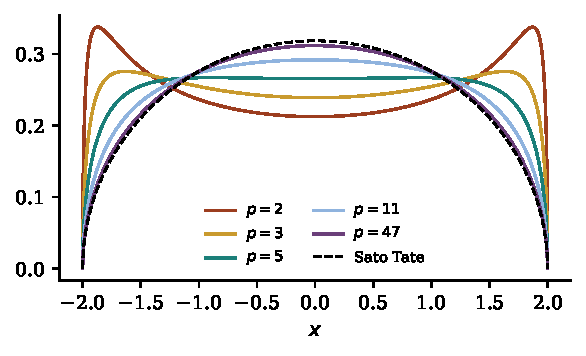
\includegraphics[width=0.85\textwidth]{figs/kestenmckay.pdf}
\caption{Densities of the Kesten McKay laws $\mu_q$ for the primes $q=2,3,5,11,47$ (labelled $p$ in the legend) against the Sato Tate semicircle (dashed). As $q$ grows the mass moves from the edges towards the centre (Theorem~\ref{thm:07tree}(6)).}\label{fig:07kestenmckay}
\end{figure}

\section{Kesten and McKay}

Statement (4) of Theorem~\ref{thm:07tree} can be rewritten as
\[
\Prob(S_{2m}=o)=\rho^{2m}\int\Bigl(\frac x2\Bigr)^{2m}d\mu_q(x),\qquad \rho=\frac{2\sqrt q}{q+1}<1,
\]
and since $\mu_q$ lives on $[-2,2]$ with a density vanishing like a square root at $\pm2$, the integral decays like $m^{-3/2}$. So return probabilities decay like $\rho^n$ up to a polynomial factor. This is Kesten's computation.

\begin{theorem}[Kesten \cite{kesten1959,kesten1959b}]\index{Kesten's theorem}
The spectral radius $\limsup_n\Prob(S_n=o)^{1/n}$ of simple random walk on the $(q+1)$ regular tree is $2\sqrt q/(q+1)$. For a symmetric random walk on a finitely generated group whose step law has finite support generating the group, the spectral radius equals $1$ if and only if the group is amenable.
\end{theorem}

The tree is a Cayley graph of the free product $(\Z/2)^{*(q+1)}$, which is not amenable. Figure~\ref{fig:07treereturn} compares exact return probabilities with $\rho^n$.

\begin{theorem}[McKay \cite{mckay1981}]\index{McKay's law}
Let $G_n$ be $(q+1)$ regular graphs on $n$ vertices such that for every fixed $k$ the number of cycles of length $k$ is $o(n)$. Then the empirical distribution of the eigenvalues of $q^{-1/2}A(G_n)$ converges weakly to $\mu_q$. The hypothesis holds with probability tending to one for uniformly random $(q+1)$ regular graphs.
\end{theorem}

McKay's proof counts closed walks: when short cycles are rare, almost every vertex sees a tree out to any fixed radius, so the empirical moments converge to those of $\mu_q$. In later language the graphs converge locally to the tree in the sense of Benjamini and Schramm \cite{benjaminischramm2001}, and local convergence implies weak convergence of the empirical spectral measures, which are the averages over vertices of the spectral measures at the $\delta_v$.\index{Benjamini Schramm convergence} We use the same argument for the vertical theorem below.

\begin{figure}[t]\centering
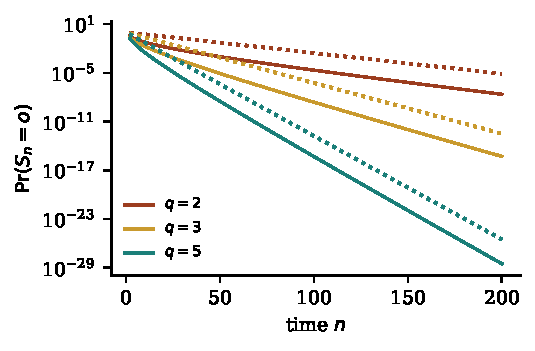
\includegraphics[width=0.7\textwidth]{figs/treereturn.pdf}
\caption{Return probabilities $\Prob(S_n=o)$ of simple random walk on $\T_q$, computed by dynamic programming on the distance chain at even times $n\le200$, for $q=2,3,5$ (solid) against the Kesten rate $(2\sqrt q/(q+1))^n$ (dotted), on a logarithmic scale. Each solid curve lies below its dotted curve by a factor of order $n^{-3/2}$.}\label{fig:07treereturn}
\end{figure}

\section{The $p$ adic Plancherel measure}\index{Plancherel measure}

The spectral theory of $A$ on $\ell^2(\T_q)$ is the spherical harmonic analysis of $\PGL_2(\Q_q)$. An irreducible unramified representation $\pi$ of $\PGL_2(\Q_q)$ has a one dimensional space of $\PGL_2(\Z_q)$ fixed vectors on which $T_q$ acts by a scalar, and by the Satake isomorphism (Theorem~\ref{thm:ch3satake}) this scalar is $q^{1/2}(\alpha+\alpha^{-1})$, where $\{\alpha,\alpha^{-1}\}$ is the Satake parameter, a semisimple conjugacy class in the dual group $\SL_2(\C)$. The representation is tempered exactly when $|\alpha|=1$, that is when $x=\alpha+\alpha^{-1}=2\cos\theta$ lies in $[-2,2]$. Thus
\[
\text{unramified tempered dual of }\PGL_2(\Q_q)\;\longleftrightarrow\;[0,\pi]\;\longleftrightarrow\;[-2,2],
\]
and, with Haar measure normalised so that $\PGL_2(\Z_q)$ has volume one, the Plancherel measure restricted to this set is $\mu_q$: for $\PGL_2(\Q_q)$, Macdonald's Plancherel formula for spherical functions \cite{macdonald1971} is the identity $\langle\delta_o,\phi(X)\delta_o\rangle=\int\phi\,d\mu_q$ with the density of Theorem~\ref{thm:07tree}(3). The nontempered parameters, including the trivial representation at $x=q^{1/2}+q^{-1/2}$ (the pole of the density), carry no Plancherel mass.

The Ramanujan conjecture for $\GL_2$ says that the local components of cuspidal automorphic representations are tempered, so their Satake parameters live in the support of $\mu_q$. For holomorphic forms of weight $k\ge2$ it is Deligne's theorem \cite{deligne1974}, in weight one it is due to Deligne and Serre \cite{deligneserre1974}, and for Maass forms it is open. In the next section the same measure appears as the limiting distribution of these parameters.

\section{The vertical Sato Tate theorem}\index{vertical Sato Tate theorem}

Fix a prime $q$. For $N\ge1$ with $q\nmid N$ and even $k\ge2$, let $x_1,\dots,x_d$ be the eigenvalues, with multiplicity, of $T_q/q^{(k-1)/2}$ on $S_k(\Gamma_0(N))$, where $d=\dim S_k(\Gamma_0(N))$; they lie in $[-2,2]$ by Deligne.

\begin{theorem}[Serre \cite{serre1997}; Conrey, Duke and Farmer \cite{cdf1997}]\label{thm:07serre}
As $k+N\to\infty$ with $k$ even and $q\nmid N$, the empirical measure $d^{-1}\sum_j\delta_{x_j}$ converges weakly to $\mu_q$.
\end{theorem}

Conrey, Duke and Farmer treated level one; Serre treated the general case, including joint equidistribution at finitely many primes.

\paragraph{Proof idea.} For $q\nmid N$ the Hecke relation $T_qT_{q^n}=T_{q^{n+1}}+q^{k-1}T_{q^{n-1}}$ gives $q^{-n(k-1)/2}T_{q^n}=U_n(x/2)$ on an eigenform whose normalised $T_q$ eigenvalue is $x$, the analogue of Exercise~\ref{ex:07hecke}. The Eichler Selberg trace formula expresses $\tr T_{q^n}$ on $S_k(\Gamma_0(N))$ as an identity term, present only for even $n$, plus elliptic terms given by class numbers of imaginary quadratic orders of discriminant $t^2-4q^n$, plus smaller hyperbolic and parabolic terms. After normalisation the identity term divided by the dimension tends to $q^{-n/2}$ for even $n$, and for fixed $n$ the other terms are of lower order than the dimension. Hence $d^{-1}\sum_jU_n(x_j/2)\to\int U_n(x/2)\,d\mu_q$ for every $n$, which gives the vertical law by the method of moments (Theorem~\ref{thm:A:moments}).

The probabilistic reading is cleanest in weight two and prime level $N\equiv1\bmod12$, where the space of forms can be realised on a finite graph. The supersingular $q$ isogeny graph $G_N(q)$ of Chapter~\ref{ch:08} has $h=(N-1)/12$ vertices, is $(q+1)$ regular, and is a finite quotient $\Gamma\backslash\T_q$ of the tree by a discrete cocompact group $\Gamma$ coming from a definite quaternion algebra. Its adjacency eigenvalues are $q+1$ together with those of $T_q$ on $S_2(\Gamma_0(N))$ (Theorem~\ref{thm:08brandt}). Identity (1) of Theorem~\ref{thm:07tree} holds on any $(q+1)$ regular graph, with $A_n$ counting nonbacktracking walks: a step appended to a nonbacktracking walk of length $n$ either extends it to one of length $n+1$ or undoes its last step, and the walks of the second kind number $q$ for each nonbacktracking walk of length $n-1$ ($q+1$ when $n=1$). Taking normalised traces,
\[
\frac1h\sum_{\lambda}\Bigl(U_n\bigl(\tfrac{\lambda}{2\sqrt q}\bigr)-q^{-1}U_{n-2}\bigl(\tfrac{\lambda}{2\sqrt q}\bigr)\Bigr)=\frac{q^{-n/2}}{h}\,\tr A_n ,
\]
which is $q^{-n/2}$ times the expected number of closed nonbacktracking walks of length $n$ from a uniformly random vertex. A closed nonbacktracking walk of length $n$ at a curve $E$ determines, up to sign, an endomorphism of $E$ of degree $q^n$ with cyclic kernel, and by Deuring and Eichler \cite{deuring1941,eichler1954,gross1987} the total number of these over all $E$ is bounded by a sum of class numbers $H(4q^n-t^2)$ that does not depend on $N$. So the right side tends to zero as $N\to\infty$: with probability tending to one, a uniformly random vertex of $G_N(q)$ sees no cycle of bounded length, that is, $G_N(q)$ converges locally to $\T_q$ in the sense of Benjamini and Schramm. The left side is an empirical version of $c_n=q^{-1}c_{n-2}$, and its limit forces the moments of $\mu_q$. In this setting the trace formula is an expectation over a uniformly random vertex of a finite quotient of the tree, its elliptic terms count short cycles, and the vertical theorem is local convergence.

\begin{remark}[Finite level correction]\label{rem:07finite}
The same identity gives the exact finite level bias. The constant eigenvector, with eigenvalue $\lambda=q+1$, contributes $q^{-n/2}(q+1)q^{n-1}/h$ to the left side, where $(q+1)q^{n-1}$ is the size of a sphere of radius $n$ in $\T_q$. Removing it, and writing $x_j=\lambda_j/\sqrt q$ for the $h-1$ normalised nontrivial eigenvalues, the average over the cusp forms is
\[
\frac{1}{h-1}\sum_{j}\Bigl(U_n(x_j/2)-q^{-1}U_{n-2}(x_j/2)\Bigr)=\frac{q^{-n/2}}{h-1}\Bigl(\tr A_n-(q+1)q^{n-1}\Bigr).
\]
For fixed $n$ both terms on the right are $O(1/h)$: the negative one is the Eisenstein contribution, the positive one counts cycles and is class number data. Call the right side $e_n$. If $\hat c_n$ is the average of $U_n(x_j/2)$ over $j$, with $\hat c_{-1}=0$, the left side is $\hat c_n-q^{-1}\hat c_{n-2}$; since $\hat c_0=c_0=1$ and $c_n=q^{-1}c_{n-2}$, induction gives $\hat c_n-c_n=\sum_{0\le k<n/2}q^{-k}e_{n-2k}$, so the balance of the two terms in $e_n,e_{n-2},\dots$ decides the sign of the correction.
\end{remark}

\subsection{Data}

We use the data set of Chapter~\ref{ch:08}, the supersingular $2$ and $3$ isogeny graphs at the $207$ primes $N\equiv1\bmod12$ between $1000$ and $8000$. For $N=1009$ and $q=3$ the nontrivial spectrum agrees with that of $T_3$ on $S_2(\Gamma_0(1009))$ computed by PARI to $10^{-13}$. Pooling the normalised nontrivial eigenvalues $x=\lambda/\sqrt q$ gives $75{,}497$ values for each $q$. Table~\ref{tab:07vertical} compares their Chebyshev averages with $c_n=q^{-n/2}$; the odd averages ($n=1,3$) lie between $-0.0041$ and $-0.0028$ for both $q$. The small deviations are the finite level correction of Remark~\ref{rem:07finite}: for $n=2$ and $q=2$ the deviation is $e_2$, whose pooled Eisenstein term is $-3\cdot207/75497=-0.0082$; the observed deviation is $-0.0040$, and the difference is the positive cycle term. At $n=8$ and $q=3$ the cycle terms win and the average exceeds its limit. Figure~\ref{fig:07vertical} shows the histograms.

\begin{table}[t]\centering\small\setlength{\tabcolsep}{4pt}
\begin{tabular}{lcccccccc}
\toprule
& \multicolumn{4}{c}{$q=2$} & \multicolumn{4}{c}{$q=3$}\\
$n$ & $2$ & $4$ & $6$ & $8$ & $2$ & $4$ & $6$ & $8$\\
\midrule
data & $0.4960$ & $0.2443$ & $0.1194$ & $0.0573$ & $0.3299$ & $0.1071$ & $0.0360$ & $0.0145$\\
$q^{-n/2}$ & $0.5$ & $0.25$ & $0.125$ & $0.0625$ & $0.3333$ & $0.1111$ & $0.0370$ & $0.0123$\\
\bottomrule
\end{tabular}
\caption{Pooled averages of $U_n(x/2)$ over the nontrivial spectra of the supersingular $q$ isogeny graphs at $207$ prime levels, against the tree moments of Theorem~\ref{thm:07tree}.}\label{tab:07vertical}
\end{table}

\begin{figure}[t]\centering
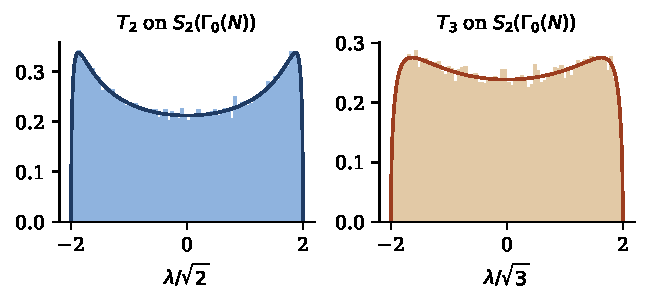
\includegraphics[width=0.9\textwidth]{figs/vertical.pdf}
\caption{Pooled normalised eigenvalues $x=\lambda/\sqrt q$ of $T_2$ (left) and $T_3$ (right) on $S_2(\Gamma_0(N))$ for the $207$ primes $N\equiv1\bmod12$ between $1000$ and $8000$ ($75{,}497$ values for each $q$), computed as nontrivial spectra of supersingular isogeny graphs, against the Kesten McKay densities $\mu_2$ and $\mu_3$.}\label{fig:07vertical}
\end{figure}

\section{Horizontal versus vertical}

There are two limits and two laws. Horizontally, a single newform $f$ without complex multiplication is fixed and $p$ varies; the Satake parameters equidistribute for $\ST$ (Theorem~\ref{thm:04STthm}). Vertically, $q$ is fixed and the form varies over a growing family; the parameters equidistribute for $\mu_q$. Theorem~\ref{thm:07tree}(6) reconciles them. The horizontal statement over primes $p\le x$ samples the local laws $\mu_p$ at ever larger $p$, which by (6) look more and more like the semicircle: the semicircle is the large degree limit of the tree, the free semicircular law of Voiculescu's theory. This is a heuristic for why the two laws are compatible, not a proof of either: the horizontal theorem needs the analytic behaviour of all symmetric power $L$ functions on $\Re s=1$, which comes from their potential automorphy \cite{blght2011}, and the vertical theorem needs the trace formula.

The vertical picture generalises to reductive groups.

\begin{theorem}[Shin \cite{shin2012}]
Let $G$ be a connected reductive group over a totally real field $F$ such that $G(F\otimes_\Q\R)$ has discrete series, under conditions on the centre. For families of cuspidal automorphic representations with level shrinking to the identity at fixed weight, or with weight tending to infinity at fixed level, the normalised counting measures of the local components at a fixed finite place $v$ converge to the Plancherel measure of $G(F_v)$ (tested against the Hecke algebra).
\end{theorem}

For $\PGL_2$ and spherical test functions the weight aspect recovers Theorem~\ref{thm:07serre} at fixed level; the level aspect concerns levels such as those of $\Gamma(N)$, which shrink to the identity, rather than $\Gamma_0(N)$. In higher rank the tree becomes a building, simple random walk becomes several commuting Hecke walks, and $\mu_q$ becomes Macdonald's measure on a torus modulo the Weyl group.

\section{Notes}

The tree of $\PGL_2(\Q_q)$ is constructed in Serre's book \emph{Trees} \cite{serre1980}, which also explains Ihara's theorem that torsion free discrete subgroups of $\SL_2(\Q_q)$ are free \cite{ihara1966}. Kesten's two papers of 1959 \cite{kesten1959,kesten1959b} gave the return probabilities on free groups and the amenability criterion. McKay \cite{mckay1981} found the same law for random regular graphs; Macdonald \cite{macdonald1971} is the reference for spherical functions. The vertical law is due to Serre \cite{serre1997} and, for level one, Conrey, Duke and Farmer \cite{cdf1997}; Sarnak \cite{sarnak1987} had earlier proved the same law for the Hecke eigenvalues of Maass forms on $\SL_2(\Z)$ ordered by Laplace eigenvalue, and Murty and Sinha \cite{murtysinha2009} gave effective versions. Shin's theorem \cite{shin2012} and its quantitative refinement by Shin and Templier \cite{shintemplier2016} put the vertical law in the general setting of the Langlands programme. The individual statements of Theorem~\ref{thm:07tree} are classical, and the recursion for the sphere operators $A_n$ is standard in the theory of Ramanujan graphs \cite{lps1988}; what is ours is the formulation and the single proof organised around the Chebyshev identity (1).

\section{Exercises}

\begin{enumerate}
\item\label{ex:07hecke} Let $T_{q^n}f([L])=\sum f([L'])$, summed over the sublattices $L'\subseteq L$ of index $q^n$, with $T_1=I$. Show that these sublattices are the $q^bL''$ with $0\le b\le n/2$ and $L/L''$ cyclic of order $q^{n-2b}$, so that $T_{q^n}=\sum_{0\le k\le n/2}A_{n-2k}$ on $\T_q$. Show that $T_qT_{q^n}=T_{q^{n+1}}+qT_{q^{n-1}}$ for $n\ge1$, and deduce $q^{-n/2}T_{q^n}=U_n(X/2)$, either from this recursion or by telescoping part (1) of Theorem~\ref{thm:07tree}.
\item Use the density in Theorem~\ref{thm:07tree}(3) and vertex transitivity to show that $\|A\|=2\sqrt q$ on $\ell^2(\T_q)$, and that $\Prob(S_{2m}=o)\sim C_q\,m^{-3/2}\rho^{2m}$; identify $C_q$.
\item Compute the generating function $G(u)=\sum_n\Prob(S_n=o)u^n$ by first passage decomposition of the distance chain and check $G(1)=q/(q-1)$. Show that the radius of convergence of $G$ is $1/\rho$, with branch points at $u=\pm1/\rho$, and relate this to Kesten's theorem.
\item Let $d=d(o,v)$, $U_{-1}=0$ and $U_{-2}=-1$. Show that the function
\[
\varphi_\theta(v)=\tfrac{q}{q+1}q^{-d/2}\bigl(U_{d}(\cos\theta)-q^{-1}U_{d-2}(\cos\theta)\bigr)
\]
satisfies $\varphi_\theta(o)=1$ and $A\varphi_\theta=2\sqrt q\cos\theta\,\varphi_\theta$. For $\theta\in\C$, show that it is bounded exactly when $|\Im\theta|\le\frac12\log q$.
\item Let $\mu_q$ be as in Theorem~\ref{thm:07tree}. Show that $\int\log(4-x^2)\,d\mu_q$ is finite and compute it, using $\log(4\sin^2\theta)=-2\sum_{k\ge1}\cos(2k\theta)/k$ and the Poisson kernel in the proof of (3); compare with $\int\log(4-x^2)\,d\ST=1$.
\end{enumerate}

\section{Open computational problems}

\begin{compproblem}[Rate of vertical convergence]
Objective: measure the rate at which the eigenvalues of $T_p$ on $S_2(\Gamma_0(N))$ approach $\mu_p$, and separate the exact finite level correction from the rest. Data: all primes $N\equiv1\bmod12$ with $37\le N<10^5$ and all primes $p\le50$ with $p\ne N$, so that Remark~\ref{rem:07finite} applies as stated, using PARI/GP \texttt{mfheckemat} for $N\le10^4$ and, beyond, sparse Brandt matrices (Sage or Magma) or supersingular isogeny graphs built as in Chapter~\ref{ch:08}. Deliverable: the Chebyshev averages $\hat c_n(N,p)$ for $n\le20$, split into the Eisenstein and class number terms of Remark~\ref{rem:07finite}, and the Kolmogorov distance to $\mu_p$ as a function of $N$, compared with the effective bounds of Murty and Sinha \cite{murtysinha2009}. Why it matters: each Chebyshev average is given exactly by the trace formula, but the Kolmogorov distance involves all $n$ at once and has no closed form; its decay, and its fluctuation from level to level, can be compared with random matrix heuristics for families (Chapter~\ref{ch:06}).
\end{compproblem}

\begin{compproblem}[Noncongruence quotients]
Objective: compare quotients of the tree by congruence and by noncongruence subgroups of one arithmetic lattice. For a prime $q\equiv1\bmod4$ the lattice $\Gamma\subset\PGL_2(\Q_q)$ of Lubotzky, Phillips and Sarnak \cite{lps1988}, built from integral Hamilton quaternions of norm a power of $q$, is free on $(q+1)/2$ generators and acts simply transitively on the vertices of $\T_q$. A subgroup of index $n$ is therefore given by a transitive action of these generators on $n$ points, and its quotient of $\T_q$ is the $(q+1)$ regular Schreier graph of that action. Data: $q=5$ and $q=13$; congruence subgroups of index up to $10^3$, such as the stabilisers of points of $\mathbb P^1(\mathbb F_M)$ under reduction of $\Gamma$ modulo odd primes $M\ne q$; for each such index, $100$ transitive actions by independent uniform random permutations, which define noncongruence subgroups with probability tending to one (GAP or Magma). Algorithm: sparse eigensolvers and $10^6$ simulated walks per graph up to time $200$. Deliverable: histograms against $\mu_q$, the largest nontrivial eigenvalue against $2\sqrt q$, and return probability curves against Figure~\ref{fig:07treereturn}. Why it matters: congruence quotients are Ramanujan by the Ramanujan bound for weight two forms, while random quotients are only nearly Ramanujan (Friedman \cite{friedman2008}); local convergence to the tree is a property of the graph, the Ramanujan property is arithmetic, and the experiment measures the gap between the two.
\end{compproblem}

\begin{compproblem}[Plancherel statistics for $\GL_3$]
Objective: test Shin's theorem in rank two. Data: quotients of the building of $\PGL_3(\Q_2)$ by cocompact arithmetic lattices, up to $10^5$ vertices, with the two commuting Hecke operators on vertices. Such lattices come from unitary groups in three variables over $\Q$ that are compact at infinity and attached to an imaginary quadratic field in which $2$ splits, so that at $2$ the projective unitary group becomes $\PGL_3(\Q_2)$. Algorithm: for the unitary group of a definite hermitian form, enumerate the genus of a hermitian lattice and compute the Hecke operators by neighbour methods (Magma), diagonalise both, and map joint eigenvalues to Satake parameters in the maximal torus of $\SU(3)$. Deliverable: histograms on the Weyl alcove against Macdonald's Plancherel density, moments of $\SU(3)$ characters, and the proportion of nontempered parameters. Why it matters: it is the first case in which the tree becomes a building, and the Ramanujan property of a quotient is no longer automatic: in Rogawski's classification of the automorphic representations of unitary groups in three variables, the endoscopic lifts of one dimensional representations have nontempered unramified local components and do occur, so the naive Ramanujan conjecture fails for general lattices of this kind, although the bound is known for all other infinite dimensional representations; the proportion of nontempered parameters detects these lifts and measures how far the quotients are from Ramanujan complexes.
\end{compproblem}

\chapter[Ihara Zeta Functions, Ramanujan Graphs and Hitting Times]{Ihara Zeta Functions,\\ Ramanujan Graphs and Hitting Times}\label{ch:08}

In 1966 Ihara attached to a discrete, torsion free, cocompact subgroup $\Gamma$ of $\PGL_2$ over a $p$ adic field with residue field of order $q$ a zeta function, an Euler product over the primitive closed geodesics of the finite quotient graph $\Gamma\backslash\T_q$, and proved that it is a rational function whose poles are governed by the eigenvalues of the Hecke operator \cite{ihara1966}. Sunada, Hashimoto and Bass later recognised that the construction makes sense for any finite graph \cite{sunada1986,hashimoto1989,bass1992}. For a regular graph the analogue of the Riemann hypothesis is a statement about eigenvalues that Lubotzky, Phillips and Sarnak, motivated by the Ramanujan conjecture, called the Ramanujan property \cite{lps1988}. We read the graph Riemann hypothesis three ways: as a statement about poles, about eigenvalues and about how fast a random walk forgets its start. We then turn to supersingular isogeny graphs, whose spectra are Hecke eigenvalues, and prove that their Kemeny constant, the expected time to hit a uniformly random target, is asymptotic to $\ell/(\ell-1)$ times the number of vertices.

\section{The Ihara zeta function}\index{Ihara zeta function}

Let $G$ be a finite connected graph, possibly with loops and multiple edges, with vertex set $V$, $n=|V|$, and edge set $E$. Orient each edge both ways, and let $A(x,y)$ count the oriented edges from $x$ to $y$, so that a loop contributes $2$ to the diagonal of the adjacency matrix $A$. A closed path $C=(e_1,\dots,e_m)$ of oriented edges is \emph{reduced} if $e_{i+1}\ne\bar e_i$ for all $i$ (indices mod $m$, so there is no backtracking and no tail), and \emph{primitive} if it is not a power $D^k$ with $k\ge2$. A \emph{prime} $\mathfrak p$ is an equivalence class of primitive reduced closed paths under cyclic rotation; its length is $\nu(\mathfrak p)$. The Ihara zeta function is
\[
Z_G(u)=\prod_{\mathfrak p}\bigl(1-u^{\nu(\mathfrak p)}\bigr)^{-1},
\]
convergent for small $|u|$. Then $u\,Z_G'(u)/Z_G(u)=\sum_{m\ge1}N_mu^m$, where $N_m$ counts reduced closed paths of length $m$: $Z_G$ counts closed nonbacktracking walks as $\zeta$ counts prime powers.

\begin{theorem}[Ihara \cite{ihara1966}; Bass \cite{bass1992}; Hashimoto \cite{hashimoto1989}]
If $G$ is $(q+1)$ regular with adjacency matrix $A$, then
\[
Z_G(u)^{-1}=(1-u^2)^{r-1}\det\bigl(I-Au+qu^2I\bigr),
\]
where $r=|E|-n+1$ is the rank of the fundamental group of $G$, so that $r-1=(q-1)n/2$.
\end{theorem}

The proof writes $N_m=\tr H^m$, where $H$ is the nonbacktracking (Hashimoto) matrix indexed by the $2|E|$ oriented edges, so that $Z_G(u)^{-1}=\det(I-uH)$, and evaluates this determinant by a block matrix identity equivalent to the recursions for $A_m$ in Theorem~\ref{thm:07tree}. For each eigenvalue $\lambda$ of $A$ the factor $1-\lambda u+qu^2$ contributes two poles $u_\pm$ with $u_+u_-=1/q$ and $u_++u_-=\lambda/q$. For $q\ge2$ the factor $(1-u^2)^{r-1}$ contributes poles at $u=\pm1$; the eigenvalue $\lambda=q+1$ gives poles at $u=1$ and $u=1/q$, and if $G$ is bipartite the eigenvalue $-(q+1)$ gives poles at $u=-1$ and $u=-1/q$. The poles in $\{\pm1,\pm1/q\}$ are the \emph{trivial} poles. In the variable $u=q^{-s}$ the pole at $u=1/q$ is $s=1$, and the circle $|u|=q^{-1/2}$ is the line $\Re s=\tfrac12$.

\begin{definition}\index{Ramanujan graph}
A $(q+1)$ regular graph satisfies the \emph{graph Riemann hypothesis} if every nontrivial pole of $Z_G$ lies on $|u|=q^{-1/2}$. It is \emph{Ramanujan} if every eigenvalue $\lambda$ of $A$ with $|\lambda|\ne q+1$ satisfies $|\lambda|\le2\sqrt q$.
\end{definition}

The name reflects the fact that for the graphs of Lubotzky, Phillips and Sarnak and for the isogeny graphs below the bound is the Ramanujan conjecture for weight two modular forms, which is a theorem: Eichler \cite{eichler1954} deduced it for prime level from Weil's Riemann hypothesis for curves over finite fields through the Eichler Shimura relation, and Deligne \cite{deligne1974} proved it in all weights. The bound $2\sqrt q$ is the edge of the support of the Kesten McKay law $\mu_q$ of Chapter~\ref{ch:07} after rescaling, and by the Alon Boppana theorem it cannot be improved for infinite families \cite{nilli1991}\index{Alon Boppana bound} (Exercise~\ref{ex:08alon} proves a weak form).

\section{Three forms of the Riemann hypothesis for graphs}

Let $P=A/(q+1)$ be the transition matrix of simple random walk on $G$; its stationary law is uniform. Order the eigenvalues of $A$ as $q+1=\lambda_1\ge\lambda_2\ge\dots\ge\lambda_n$, let $\mu_j=\lambda_j/(q+1)$, and define
\[
\lambda_*=\max\{|\lambda_j|:|\lambda_j|\ne q+1\},\qquad \delta_t=\max_{x\in V}\Bigl|P^t(x,x)-\frac{1+\beta(-1)^t}{n}\Bigr|,
\]
where $\beta=1$ if $G$ is bipartite and $\beta=0$ otherwise, and $\lambda_*=0$ if no eigenvalue has $|\lambda_j|\ne q+1$. Thus $\delta_t$ measures how far return probabilities are from their stationary (or, in the bipartite case, periodic stationary) values. Write $\rho_q=2\sqrt q/(q+1)$ for the Kesten rate of the tree (Chapter~\ref{ch:07}).

\begin{proposition}[this book]\label{prop:08three}\index{graph Riemann hypothesis}
For a connected $(q+1)$ regular graph $G$ the following are equivalent.
\begin{enumerate}
\item $Z_G$ satisfies the graph Riemann hypothesis.
\item $G$ is Ramanujan.
\item $\limsup_{t\to\infty}\delta_t^{1/t}\le\rho_q$.
\end{enumerate}
Moreover $\limsup_t\delta_t^{1/t}=\lambda_*/(q+1)$ exactly, so the return probabilities of a Ramanujan graph approach equilibrium at an exponential rate no slower than the rate $\rho_q$ at which the return probabilities of the tree tend to zero.
\end{proposition}

\begin{proof}
(1)$\Leftrightarrow$(2). By the Ihara Bass formula every pole of $Z_G$ is $\pm1$ or a root of $1-\lambda_ju+qu^2$ for some $j$, and every such root is a pole. If $|\lambda_j|\le2\sqrt q$ the discriminant $\lambda_j^2-4q$ is nonpositive, the roots are complex conjugates (or a double real root) and $|u_\pm|^2=u_+u_-=1/q$. If $2\sqrt q<|\lambda_j|<q+1$, the roots are real and distinct with product $1/q$, so one of them has modulus strictly less than $q^{-1/2}$; neither is trivial, since $\pm1$ or $\pm1/q$ is a root only when $\lambda_j=\pm(q+1)$. The eigenvalues $\pm(q+1)$ give only trivial poles. Hence all nontrivial poles lie on the circle if and only if every $\lambda_j$ with $|\lambda_j|\ne q+1$ satisfies $|\lambda_j|\le2\sqrt q$.

(2)$\Leftrightarrow$(3). Let $\phi_1,\dots,\phi_n$ be an orthonormal eigenbasis of $A$ in $\ell^2(V)$ with $\phi_1\equiv n^{-1/2}$. Then $P^t(x,x)=\sum_j\mu_j^t\phi_j(x)^2$ and $\sum_j\phi_j(x)^2=1$. Since $G$ is connected, $\lambda_1=q+1$ is simple, and $-(q+1)$ is an eigenvalue (then simple, with eigenvector $n^{-1/2}(\pm1)$ on the two sides) if and only if $G$ is bipartite. Removing these terms,
\[
P^t(x,x)-\frac{1+\beta(-1)^t}{n}=\sum_{j\in J}\mu_j^t\phi_j(x)^2,
\]
where $J$ indexes the eigenvalues with $|\lambda_j|\ne q+1$. The right side is bounded in absolute value by $(\lambda_*/(q+1))^t$, so $\limsup\delta_t^{1/t}\le\lambda_*/(q+1)$. Conversely, for even $t$ all terms are nonnegative, and averaging over $x$,
\[
\delta_t\ge\frac1n\sum_x\sum_{j\in J}\mu_j^t\phi_j(x)^2=\frac1n\sum_{j\in J}\mu_j^t\ge\frac1n\Bigl(\frac{\lambda_*}{q+1}\Bigr)^t,
\]
so $\limsup\delta_t^{1/t}\ge\lambda_*/(q+1)$. Hence the limsup equals $\lambda_*/(q+1)$, and it is at most $\rho_q=2\sqrt q/(q+1)$ if and only if $\lambda_*\le2\sqrt q$.
\end{proof}

The Riemann hypothesis for $Z_G$ is therefore a statement about mixing. Applied to off diagonal entries, the same argument gives the uniform bound $|P^t(x,y)-1/n|\le(\lambda_*/(q+1))^t$ in the nonbipartite case (Appendix~\ref{app:A}), so $\max_{x,y}|nP^t(x,y)-1|\le\varepsilon$ once $t\ge\log(n/\varepsilon)/\log((q+1)/\lambda_*)$.

\section{Supersingular isogeny graphs}\index{supersingular isogeny graph}

Let $N$ be a prime and $\ell\ne N$ another prime. Every supersingular elliptic curve over $\overline{\mathbb F}_N$ has a model over $\mathbb F_{N^2}$, and there are finitely many up to isomorphism; by Deuring \cite{deuring1941} and Eichler's mass formula, when $N\equiv1\bmod12$ there are exactly $h=(N-1)/12$ of them and none has automorphisms other than $\pm1$. The supersingular $\ell$ isogeny graph $G_N(\ell)$ has these $h$ curves (or their $j$ invariants) as vertices, with an edge for each of the $\ell+1$ subgroups of order $\ell$ of a curve, joining it to the quotient curve. Dual isogenies pair edges, so for $N\equiv1\bmod12$ the graph is undirected and $(\ell+1)$ regular, possibly with loops and multiple edges. The neighbours of $j$ are the roots in $\mathbb F_{N^2}$ of the modular polynomial $\Phi_\ell(j,Y)$, counted with multiplicity, as in Mestre's \emph{m\'ethode des graphes} \cite{mestre1986}.

Through Deuring's correspondence the vertices are also the left ideal classes of a maximal order $\mathcal O$ in the definite quaternion algebra $B$ ramified at $N$ and $\infty$, and the adjacency matrix of $G_N(\ell)$ is the Brandt matrix $B(\ell)$ \cite{eichler1954,gross1987}.\index{Brandt matrix} The graph is a quotient $\Gamma\backslash\T_\ell$ of the Bruhat Tits tree of Chapter~\ref{ch:07}, with $\Gamma$ the image of $(\mathcal O[1/\ell])^\times$ in $\PGL_2(\Q_\ell)$.

A loop at a curve $E$ is an endomorphism of degree $\ell$, up to sign. When its dual has the same kernel, the loop is a \emph{half loop}: one oriented edge equal to its own reverse, entered once on the diagonal of $B(\ell)$, and it comes from an element of $\Gamma$ that inverts an edge of the tree. For $\ell=2$ and $N\equiv1\bmod12$ this happens only at the curve with $j=8000$, which has complex multiplication by $\Z[\sqrt{-2}]$ and is supersingular exactly when $N\equiv13\bmod24$; then $h$ is odd, and a $3$ regular graph on an odd number of vertices must have a half loop. (For $\ell=3$ and $N\equiv1\bmod12$ there are none.) For a $(q+1)$ regular graph with $s$ half loops the Ihara Bass formula becomes
\[
Z_G(u)^{-1}=(1-u)^{((q-1)n-s)/2}(1+u)^{((q-1)n+s)/2}\det\bigl(I-Au+qu^2I\bigr).
\]
To see this, let $\Sigma$ be the matrix with rows indexed by the vertices and columns by the $(q+1)n$ oriented edges, with $\Sigma(v,e)=1$ if $e$ starts at $v$, and let $R$ be the permutation matrix of the reversal $e\mapsto\bar e$, which has $s$ fixed points. Then $\Sigma\Sigma^{\top}=(q+1)I$ and $\Sigma R\Sigma^{\top}=A$, and $H=R\Sigma^{\top}\Sigma-R$, because $f$ follows $e$ exactly when $f$ starts at the origin of $\bar e$ and $f\ne\bar e$. Since $(I+uR)^{-1}R=(R-uI)/(1-u^2)$, the identity $\det(I-XY)=\det(I-YX)$ gives
\[
\begin{aligned}
\det(I-uH)&=\det(I+uR)\det\bigl(I-u\Sigma(I+uR)^{-1}R\Sigma^{\top}\bigr)\\
&=\det(I+uR)\,\frac{\det(I-Au+qu^2I)}{(1-u^2)^n},
\end{aligned}
\]
and $\det(I+uR)=(1-u^2)^{((q+1)n-s)/2}(1+u)^s$, because $I+uR$ is block diagonal with a block $\bigl(\begin{smallmatrix}1&u\\u&1\end{smallmatrix}\bigr)$ for each pair $\{e,\bar e\}$ and the entry $1+u$ for each half loop. Hence only the trivial poles change, and Proposition~\ref{prop:08three} applies to every $G_N(\ell)$.

\begin{theorem}[Eichler; Jacquet Langlands; Pizer \cite{eichler1954,jacquetlanglands1970,pizer1990}]\label{thm:08brandt}
For $N\equiv1\bmod12$ the spectrum of the adjacency matrix of $G_N(\ell)$ is $\{\ell+1\}$ together with the eigenvalues, with multiplicity, of $T_\ell$ on $S_2(\Gamma_0(N))$. In particular $G_N(\ell)$ is Ramanujan.
\end{theorem}

The eigenvalue $\ell+1$ belongs to the Eisenstein series, and the dimension $h-1$ of $S_2(\Gamma_0(N))$ is the genus of $X_0(N)$. The cuspidal part is Eichler's basis problem, in modern terms the Jacquet Langlands correspondence between $B^\times$ and $\GL_2$ (Chapter~\ref{ch:03}). The Ramanujan property is the bound $|a_\ell(f)|\le2\sqrt\ell$ for weight two newforms, and connectivity follows because $\ell+1$ is then simple. Lubotzky, Phillips and Sarnak \cite{lps1988} and independently Margulis \cite{margulis1988} built Ramanujan Cayley graphs of $\PGL_2$ and $\mathrm{PSL}_2$ over finite fields from Hamilton quaternions with the same input, and Morgenstern \cite{morgenstern1994} extended the construction to every prime power $q$.

\subsection{Data}

For this book we built $G_N(2)$ and $G_N(3)$ explicitly with PARI/GP \cite{pari2023} for all $207$ primes $N\equiv1\bmod12$ between $1000$ and $8000$, with $h$ from $84$ to $666$ (code in Appendix~\ref{app:B}). For every level and both $\ell$, every nontrivial pole of $Z_G$ satisfies $\bigl||u|-\ell^{-1/2}\bigr|<5\times10^{-16}$, and $\lambda_*/(2\sqrt\ell)$ is at most $0.99978$ for $\ell=2$ and $0.99983$ for $\ell=3$. Theorem~\ref{thm:08brandt} guarantees both statements, so these numbers check the computation rather than the theory. Figure~\ref{fig:08isogeny} draws $G_{1009}(2)$.

\begin{figure}[t]\centering
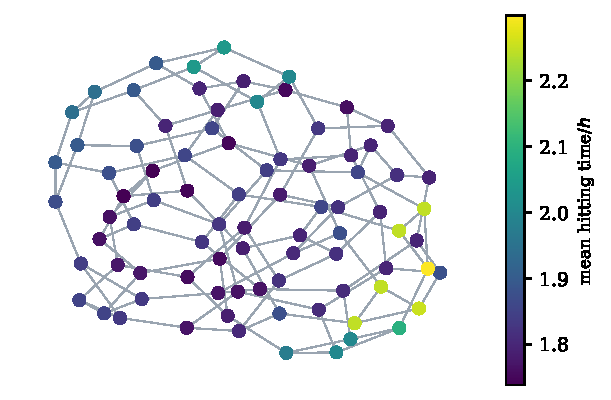
\includegraphics[width=0.7\textwidth]{figs/isogeny.pdf}
\caption{The supersingular $2$ isogeny graph for $N=1009$: $84$ vertices, $3$ regular, without loops or multiple edges. Each vertex $y$ is coloured by $\E_\pi\tau_y/h$, its mean hitting time from a uniformly random start divided by $h$; the average over all $y$ is the Kemeny constant divided by $h$, $1.866$.}\label{fig:08isogeny}
\end{figure}

\section{Random regular graphs}

Alon conjectured that random regular graphs are almost Ramanujan, and Friedman proved it.

\begin{theorem}[Friedman \cite{friedman2008}]
Fix $d\ge3$ and $\varepsilon>0$. With probability tending to one as $n\to\infty$ ($n$ even if $d$ is odd), a uniformly random $d$ regular graph on $n$ vertices has all eigenvalues other than $d$ in $[-2\sqrt{d-1}-\varepsilon,\,2\sqrt{d-1}+\varepsilon]$.
\end{theorem}

Bordenave \cite{bordenave2020} gave a shorter proof through the nonbacktracking matrix $H$ that defines the Ihara zeta function, and extended the theorem to random lifts of a fixed graph. Marcus, Spielman and Srivastava \cite{mss2015,mss2018} proved by interlacing polynomials that bipartite Ramanujan multigraphs exist for every degree and every even number of vertices. Huang, McKenzie and Yau \cite{hmy2024} showed, in a 2024 preprint, that the extreme nontrivial eigenvalues of a random $d$ regular graph fluctuate around $\pm2\sqrt{d-1}$ on the scale $n^{-2/3}$ with the Tracy Widom law of the Gaussian orthogonal ensemble; a consequence is that the probability that a random $d$ regular graph is Ramanujan tends to a constant strictly between $0$ and $1$ (their analysis puts it near $69$ percent). In a computation for this book a random $4$ regular graph on $3000$ vertices had $\lambda_*=3.46376$, just below $2\sqrt3=3.46410$, so that sample is Ramanujan.

\section{Hitting times and Kemeny's constant}\index{Kemeny constant}\index{hitting time}

For simple random walk on $G$ let $h(x,y)=\E_x\tau_y$ with $\tau_y=\min\{t\ge0:X_t=y\}$, as in Appendix~\ref{app:A}; the letter $h$ without arguments keeps its meaning as the number of vertices of an isogeny graph. Kemeny's constant $K=\sum_y\pi(y)h(x,y)$ does not depend on $x$, and for a connected $(q+1)$ regular graph (Theorem~\ref{thm:A:kemeny})
\[
K=\sum_{j\ge2}\frac{1}{1-\lambda_j/(q+1)}=\sum_{t\ge0}\Bigl(\sum_{x}P^t(x,x)-1\Bigr),
\]
where the second form, obtained by expanding each term as a geometric series, requires $G$ not to be bipartite. Since $\pi$ is uniform, $K$ is also the average of $h(x,y)$ over all ordered pairs. The mean hitting time of a fixed target from a uniform start, $\E_\pi\tau_y=n^{-1}\sum_xh(x,y)$, does depend on $y$ (Figure~\ref{fig:08isogeny}); its average over $y$ is $K$.

By the second form, $K/n$ is the expected number of visits to the starting point in excess of equilibrium, averaged over starting points. On the tree the expected number of visits to the start is the Green function $G(1)=q/(q-1)$ of Theorem~\ref{thm:07tree}(5). A graph that looks like a tree from almost every vertex should therefore have $K\approx G(1)\,n$. For isogeny graphs this heuristic is a theorem.

\begin{theorem}[Kemeny constant of isogeny graphs, this book]\label{thm:08kemeny}
Let $\ell$ be prime and let $K_N$ be the Kemeny constant of simple random walk on $G_N(\ell)$, with $h=(N-1)/12$ vertices. As $N\to\infty$ through primes $N\equiv1\bmod12$,
\[
\frac{K_N}{h}\longrightarrow\frac{\ell}{\ell-1}.
\]
Equivalently, the mean hitting time of a uniformly random target, from any fixed start or from a uniformly random one, is asymptotic to $\ell h/(\ell-1)$; for $\ell=2$ it is about $2h$.
\end{theorem}

\begin{proof}
By Theorem~\ref{thm:08brandt} the eigenvalues of the adjacency matrix are $\ell+1$ and $\lambda_j=\sqrt\ell\,x_j$ for $2\le j\le h$, where $x_2,\dots,x_h$ are the normalised eigenvalues of $T_\ell$ on $S_2(\Gamma_0(N))$, counted with multiplicity; by the Ramanujan bound they lie in $[-2,2]$. Since $|\lambda_j|\le2\sqrt\ell<\ell+1$ the graph is connected and not bipartite, and Theorem~\ref{thm:A:kemeny} gives
\[
\frac{K_N}{h}=\frac{h-1}{h}\cdot\frac{1}{h-1}\sum_{j=2}^hg(x_j),\qquad g(x)=\Bigl(1-\frac{\sqrt\ell\,x}{\ell+1}\Bigr)^{-1}.
\]
On $[-2,2]$ we have $\sqrt\ell|x|/(\ell+1)\le\rho_\ell<1$, so $g$ is continuous there, with values in $[1/(1+\rho_\ell),1/(1-\rho_\ell)]$. By the vertical Sato Tate theorem (Theorem~\ref{thm:07serre}, weight $2$, prime level $N\to\infty$, $\ell\nmid N$) the empirical measures $\nu_N=(h-1)^{-1}\sum_{j=2}^h\delta_{x_j}$ converge weakly to the Kesten McKay law $\mu_\ell$. All these measures live on the compact interval $[-2,2]$, where $g$ is continuous, so $\int g\,d\nu_N\to\int g\,d\mu_\ell$, that is,
\[
\frac{1}{h-1}\sum_{j=2}^hg(x_j)\longrightarrow\int_{-2}^2g\,d\mu_\ell .
\]
It remains to evaluate the integral. With $q=\ell$, $g$ is the integrand of the spectral expression for the Green function given after the proof of Theorem~\ref{thm:07tree}, so $\int_{-2}^2g\,d\mu_\ell=G(1)=\ell/(\ell-1)$ by Theorem~\ref{thm:07tree}(5). Since $(h-1)/h\to1$, the theorem follows. The statement about mean hitting times is the identity $K=n^{-2}\sum_{x,y}h(x,y)$ for uniform $\pi$.
\end{proof}

Without the Ramanujan bound the proof would fail: the trivial bound $|x_j|\le(\ell+1)/\sqrt\ell$ does not keep the $x_j$ away from the pole of $g$ at $(\ell+1)/\sqrt\ell$. Chapter~\ref{ch:hit} reads the terms arithmetically. By the Eichler Shimura congruence relation $\prod_{j\ge2}(\ell+1-\lambda_j)=|J_0(N)(\mathbb F_\ell)|$, and $\ell+1-\lambda_j$ is the number of points modulo $\ell$ of an elliptic curve of conductor $N$ when the eigenform has rational coefficients; so $K_N=(\ell+1)\sum_{j\ge2}(\ell+1-\lambda_j)^{-1}$ is a harmonic sum of these factors of $|J_0(N)(\mathbb F_\ell)|$ (Theorem~\ref{thm:hitkemeny}), and $G_N(\ell)$ has $|J_0(N)(\mathbb F_\ell)|/h$ spanning trees, a formula of Hashimoto (Theorem~\ref{thm:hittrees}).

\begin{remark}[An exact series]\label{rem:08exact}
The generating function $\sum_{m\ge0}U_m(x/2)z^m=(1-xz+z^2)^{-1}$ at $z=\ell^{-1/2}$ gives $g(x)=\frac{\ell+1}{\ell}\sum_{m\ge0}\ell^{-m/2}U_m(x/2)$, uniformly on $[-2,2]$ because $|U_m(x/2)|\le m+1$ there. Since $T_\ell T_{\ell^m}=T_{\ell^{m+1}}+\ell T_{\ell^{m-1}}$ on $S_2(\Gamma_0(N))$ for $\ell\nmid N$, as on the tree (Exercise~\ref{ex:07hecke} of Chapter~\ref{ch:07}), the eigenvalue of $T_{\ell^m}$ on the $j$th eigenform is $\ell^{m/2}U_m(x_j/2)$, and therefore
\[
K_N=\frac{\ell+1}{\ell}\sum_{m\ge0}\ell^{-m}\tr\bigl(T_{\ell^m}\mid S_2(\Gamma_0(N))\bigr).
\]
Dividing by $h-1$ and letting $N\to\infty$ term by term (Theorems~\ref{thm:07serre} and~\ref{thm:07tree}(2), with $|U_m(x/2)|\le m+1$) gives, by dominated convergence with the summable bound $(m+1)\ell^{-m/2}$, the limit $\frac{\ell+1}{\ell}\sum_{k\ge0}\ell^{-2k}=\frac{\ell}{\ell-1}$ again. The Eichler Selberg trace formula writes each trace through class numbers, so this series is the natural route to the second order term (Computational Problem~\ref{cp:08second}).
\end{remark}

\subsection{Spectral bounds}

The Ramanujan property also gives uniform bounds valid at every level. Write $\mu_*=\lambda_*/(\ell+1)\le\rho_\ell$, as in Appendix~\ref{app:A}. Since $1/(1+\mu_*)\le1/(1-\mu_j)\le1/(1-\mu_*)$ for $j\ge2$,
\[
\frac{h-1}{1+\rho_\ell}\le K_N\le\frac{h-1}{1-\rho_\ell}.
\]
For individual pairs, with $n=h$, the representation $h(x,y)=n\bigl(Z(y,y)-Z(x,y)\bigr)$ of Appendix~\ref{app:A}, where $\Pi$ is the matrix whose rows all equal $\pi$ and $Z=\sum_t(P^t-\Pi)$, and the bound $|P^t(x,y)-1/n|\le\mu_*^t$ give
\[
\max_{x,y}h(x,y)\le n\sum_{t\ge0}\bigl(|P^t(y,y)-\tfrac1n|+|P^t(x,y)-\tfrac1n|\bigr)\le\frac{2n}{1-\rho_\ell}.
\]
For $\ell=2$ these read $0.51(h-1)\le K_N\le17.5(h-1)$ and $\max h(x,y)\le35h$, while Theorem~\ref{thm:08kemeny} gives $K_N\sim2h$.

\subsection{Data}

For each of the $207$ levels we computed $K_N$ from the spectrum. For $\ell=2$, $K_N/h$ rises from $1.866$ at $h=84$ and lies between $1.971$ and $2.012$ for all $59$ levels with $h\ge500$ (mean $1.988$). For $\ell=3$, $K_N/h$ lies between $1.435$ and $1.515$ throughout, approaching $3/2$. A least squares fit of $a+c/h$ over all levels gives $a=2.004$, $c=-8.2$ for $\ell=2$ and $a=1.498$, $c=-3.0$ for $\ell=3$, consistent with the limits. The scatter about the fit is of the same order as the correction, and it is arithmetic: for $\ell=2$ the mean of $K_N-2h$ is $-3.3$ over the $108$ levels inert in $\Q(\sqrt{-7})$ and $-11.0$ over the other $99$. At the inert levels the curves with complex multiplication by orders of $\Q(\sqrt{-7})$ are supersingular, and the largest single contribution to the difference comes from the one with $j=-3375$ described below. Whether $K_N-2h$ stays bounded is Open Problem~\ref{op:kemeny} of Chapter~\ref{ch:13}. Figure~\ref{fig:08kemeny} shows the convergence.

As an independent check we solved the hitting time equations directly for every target on $G_N(2)$ for $N=1009,2017,4129$ ($h=84,168,344$). The Kemeny constants are $156.766$, $324.736$ and $682.586$, so that $K_N/h=1.866$, $1.933$, $1.984$, and they agree with the spectral formula to a relative error below $10^{-13}$. The maximal hitting times divided by $h$ are $2.58$, $3.35$ and $5.98$, far below the bound $35$; they reflect the neighbourhood of the hardest target, not growth in $h$. At $N=4129$ that target is the curve with $j=-3375$, which has complex multiplication by the maximal order of $\Q(\sqrt{-7})$ and is supersingular because $4129$ is inert in that field. Its endomorphisms $(1\pm\sqrt{-7})/2$ of degree $2$ form a loop counted twice, so the walk stays put with probability $2/3$. If the rest of its neighbourhood is a tree, a walk started there returns with probability $\frac23+\frac13\cdot\frac12=\frac56$ and makes $6$ visits on average, against $G(1)=2$ at a vertex whose neighbourhood is a tree, so its mean hitting time is about $6h$ (Exercise~\ref{ex:08target}). At $N=2017$ the hardest targets are the two curves with complex multiplication by the maximal order of $\Q(\sqrt{-15})$, which are joined by a double edge.

\begin{figure}[t]\centering
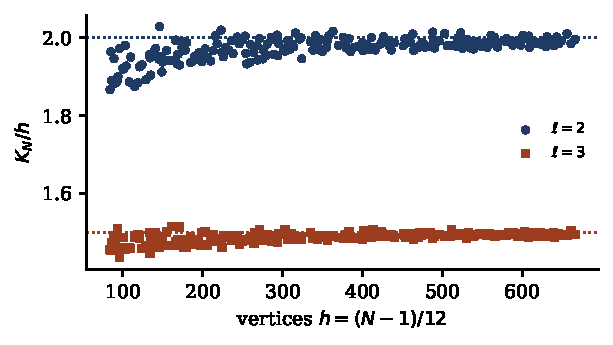
\includegraphics[width=0.75\textwidth]{figs/kemeny.pdf}
\caption{Kemeny constants $K_N$ of the supersingular $\ell$ isogeny graphs for $\ell=2,3$ at the $207$ primes $N\equiv1\bmod12$ between $1000$ and $8000$, divided by the number of vertices $h=(N-1)/12$, against the limits $2$ ($\ell=2$) and $3/2$ ($\ell=3$) of Theorem~\ref{thm:08kemeny} (dotted lines).}\label{fig:08kemeny}
\end{figure}

\section{Isogeny graphs in cryptography}

Charles, Goren and Lauter \cite{cgl2009} proposed a hash function built from walks on $G_N(2)$: the bits of the message choose, at each step, one of the two edges that do not backtrack, starting from a fixed curve, and the hash value is the endpoint. Because the graph is Ramanujan, a walk of $O(\log N)$ steps ends at a nearly uniform vertex. A collision gives two distinct paths between the same curves, hence a cycle and an endomorphism of the starting curve that is not multiplication by an integer, so security rests on the presumed difficulty of finding paths in the graph. Under the generalized Riemann hypothesis this problem is equivalent to computing endomorphism rings of supersingular curves \cite{wesolowski2022}. All known classical algorithms for it take time exponential in $\log N$; the method of Delfs and Galbraith \cite{delfsgalbraith2016} takes about $\sqrt N$ steps up to logarithmic factors. We make no claim about particular schemes and note only that the key exchange SIDH of Jao and De Feo \cite{jaodefeo2011}, which also publishes the images of torsion points under the secret isogeny, was broken in 2022 by an attack that exploits this extra information and does not solve the general path problem \cite{castryckdecru2023}. Theorem~\ref{thm:08kemeny} quantifies the cost of naive search: from any fixed start, a random walk looking for a target curve chosen uniformly at random needs $K_N\approx2h\approx N/6$ steps on average, far more than $\sqrt N$.

\section{Notes}

Ihara's zeta function appeared in his work on discrete subgroups of $p$ adic groups \cite{ihara1966}; Serre's book \cite{serre1980} made the link with graphs explicit, Sunada \cite{sunada1986} suggested general graphs, and Hashimoto \cite{hashimoto1989} and Bass \cite{bass1992} proved the determinant formula in general. Terras's book \cite{terras2011} is an introduction. The equivalence of the graph Riemann hypothesis and the Ramanujan property is standard; the third form in Proposition~\ref{prop:08three} is a reformulation we find useful because it ties the Riemann hypothesis to the Kesten rate. Supersingular graphs go back to Deuring, Eichler and Mestre \cite{mestre1986}; Pizer \cite{pizer1990} identified them as Ramanujan graphs, and Gross \cite{gross1987} used Brandt matrices for special values of $L$ functions. Kemeny and Snell \cite{kemenysnell1960} introduced the constant that bears Kemeny's name. Theorem~\ref{thm:08kemeny} is new as far as we know; it is a direct consequence of Serre's theorem once the Kemeny constant is recognised as a spectral statistic whose tree value is the gambler's ruin constant. The same constant appears for random regular graphs: Cooper and Frieze \cite{cooperfrieze2005} proved that the cover time of a random $r$ regular graph is asymptotic to $\frac{r-1}{r-2}\,n\log n$, through hitting times of order $\frac{r-1}{r-2}\,n$ at vertices whose neighbourhoods are trees, and $\frac{r-1}{r-2}=\frac{\ell}{\ell-1}$ when $r=\ell+1$.

\section{Exercises}

\begin{enumerate}
\item Prove that $u\,Z_G'(u)/Z_G(u)=\sum_mN_mu^m$. For a $(q+1)$ regular graph deduce from the Ihara Bass formula that $N_m=\sum_j(\alpha_j^m+\beta_j^m)+(|E|-n)(1+(-1)^m)$, where $\alpha_j,\beta_j$ are the roots of $t^2-\lambda_jt+q$.
\item For the complete graph on $q+2$ vertices compute $Z_G$, verify the graph Riemann hypothesis, and check $K=(n-1)^2/n$.
\item Show that a connected $(q+1)$ regular graph with $q\ge2$ is bipartite if and only if $-(q+1)$ is an eigenvalue, and that $u=-1/q$ is a pole of $Z_G$ exactly in that case. Find the order of the pole of $Z_G$ at $u=-1$ in both cases.
\item\label{ex:08alon} Prove the Alon Boppana bound in the weak form $\liminf\lambda_*\ge2\sqrt q$ for a sequence of $(q+1)$ regular graphs with $n\to\infty$. (Hint: by the recursions of Theorem~\ref{thm:07tree}(1), which hold on any $(q+1)$ regular graph, $A^{2k}$ is a combination with nonnegative coefficients of the nonbacktracking matrices $A_m$, whose traces are nonnegative, and the coefficient of $A_0=I$ is the number $q^k\int x^{2k}\,d\mu_q$ of closed walks of length $2k$ at a vertex of the tree. Compare with $\tr A^{2k}\le2(q+1)^{2k}+n\lambda_*^{2k}$, which allows for a bipartite graph, and let $k\to\infty$ slowly with $n$.)
\item\label{ex:08target} Show that for every target $y$, $\E_\pi\tau_y=\frac1n\sum_xh(x,y)=n\,Z(y,y)$, and interpret $Z(y,y)$ as an excess number of visits. For $q=2$, compute the expected number of visits to $y$ of simple random walk started at $y$ on an infinite $3$ regular graph that is a tree except that $y$ carries a loop counted twice, and compare with $G(1)=2$ and with the hardest target at $N=4129$. Do the same when $y$ carries a half loop instead, and when $y$ is joined to a neighbour by a double edge (answers $6$, $3$ and $10/3$).
\end{enumerate}

\section{Open computational problems}

\begin{compproblem}[Second order term of the Kemeny constant]\label{cp:08second}
Objective: determine the correction $K_N-\ell h/(\ell-1)$ as a function of $N$. Data: all primes $N\equiv1\bmod12$ up to $10^6$, $\ell=2,3$. Algorithm: the series of Remark~\ref{rem:08exact}, with $\tr T_{\ell^m}$ from the Eichler Selberg trace formula, whose elliptic term is a sum of Hurwitz class numbers $H(4\ell^m-s^2)$ weighted by Legendre symbols at $N$ and whose identity, hyperbolic and weight two divisor terms are explicit (the identity term, $(N+1)/12$ for even $m$, contributes $\ell/(6(\ell-1))$ to the correction); the class numbers do not depend on $N$ and can be tabulated once, and the series is truncated at $m$ of order $\log N$. Check against PARI/GP spectra for $N\le10^5$. Deliverable: the empirical law of the correction, its regression on the symbols $(D/N)$ for small discriminants $D$, and a conjectural formula in terms of class numbers. Why it matters: the correction is where the elliptic terms, invisible in the limit, become measurable; it explains the scatter in Figure~\ref{fig:08kemeny}, which for $\ell=2$ is led by $D=-7$, and it is the computational side of Open Problem~\ref{op:kemeny} of Chapter~\ref{ch:13}.
\end{compproblem}

\begin{compproblem}[Hitting times on large supersingular graphs]
Objective: the distribution over targets $y$ of the mean hitting time $\E_\pi\tau_y/h=Z(y,y)$ on $G_N(2)$, and of $\max_{x,y}h(x,y)/h$, which the spectral bound keeps below $35$. Data: $G_N(2)$ for $N$ up to $10^7$ ($h$ near $8\times10^5$), walks generated on the fly from $\Phi_2$ over $\mathbb F_{N^2}$. Algorithm: $10^5$ Monte Carlo walks per level on GPU, run in continuous time with exponential holding times of mean one, which leaves the means unchanged, with exact sparse solves for $N\le10^5$ as ground truth. Deliverable: histograms of $\E_\pi\tau_y/h$ over targets, with the atoms predicted by Exercise~\ref{ex:08target}, and the law of $\tau_y/\E_\pi\tau_y$ against the exponential law that Corollary~\ref{cor:10cisogeny} of Chapter~\ref{ch:10c} guarantees up to $O(1/h)$. Why it matters: the exponential law predicts the cost of naive search once the mean is known, and the means carry the arithmetic, through curves with complex multiplication by small discriminants.
\end{compproblem}

\begin{compproblem}[Other degrees and ordinary curves]
Objective: repeat the analysis for $\ell=5,7$ and for $\ell$ isogeny graphs of ordinary curves. Data: supersingular $G_N(\ell)$ for $N\le10^5$; ordinary isogeny volcanoes over $\mathbb F_N$ for $N\le10^6$ (Sutherland's algorithms or Sage). Deliverable: $K_N/h$ against $\ell/(\ell-1)$, and for volcanoes the Kemeny constant as a function of the class group and the depth. Why it matters: volcanoes are governed by class groups of imaginary quadratic orders rather than by the Ramanujan bound, so the comparison isolates what Theorem~\ref{thm:08kemeny} owes to the Ramanujan property.
\end{compproblem}

\begin{compproblem}[Ihara zeta as a test for random lifts]
Objective: the probability that a random $k$ fold lift of $G_N(2)$ satisfies the graph Riemann hypothesis for its new poles. Data: lifts of index $k\le100$ of graphs with $h\le500$, $10^4$ lifts each. Algorithm: largest new eigenvalue of the nonbacktracking matrix $H$ by sparse Arnoldi iteration. Deliverable: the empirical probability as a function of $k$ and $h$, with Tracy Widom fits at the edge. Why it matters: Bordenave proved that random lifts are almost Ramanujan; whether lifts of arithmetic graphs behave like random graphs probes how much arithmetic survives a random perturbation.
\end{compproblem}

\part{L\'evy and Thorin Measures}
\chapter{Infinite Divisibility of Euler Products}\label{ch:09}

In his 1938 monograph on limit laws for sums of independent random variables, Khinchine observed that the Riemann zeta function, read along a vertical line to the right of $1$ and divided by its value on the real axis, is the characteristic function of an infinitely divisible law. The proof is one line long: the logarithm of an Euler product is a sum over prime powers, and a sum of exponentials with positive weights is the exponent of a compound Poisson law. This chapter develops two consequences. First, positivity of the weights, which for automorphic $L$ functions is the positivity of Rankin Selberg convolutions, underlies the usual proofs of nonvanishing on the line $\operatorname{Re} s = 1$ and of the classical zero free regions; for the standard $L$ function of a cusp form the weights change sign and the characteristic function property fails. Second, once $p^{-it}$ is replaced by an independent uniform phase, the logarithm of an Euler product becomes a sum of independent random variables, and the theory of Bohr and Jessen describes the values of $\zeta$ to the right of the critical line by the law of that sum. We carry the first picture to $\GL_n$ and the second to $\GL_2$, where the natural random model draws Satake parameters from the Sato Tate measure, and we compute what Sato Tate implies for the law of that model.

\section{Infinitely divisible laws}

A probability law $\mu$ on $\R$ is \emph{infinitely divisible}\index{infinitely divisible law} if for every $n$ it is the $n$ fold convolution power of some probability law $\mu_n$. The class is closed under convolution and weak limits, and it is described completely by the following theorem.

\begin{theorem}[L\'evy Khintchine]\label{thm:ch09lk}
A function $\varphi:\R\to\C$ is the characteristic function of an infinitely divisible law if and only if $\varphi = e^{\eta}$ with
\[
\eta(t) = i a t - \tfrac12 \beta^2 t^2 + \int \bigl(e^{itx} - 1 - itx\,1_{\{|x|<1\}}\bigr)\,\nu(dx)
\]
for some $a\in\R$, some $\beta \ge 0$ and some positive measure $\nu$ on $\R\setminus\{0\}$ satisfying $\int \min(1,x^2)\,\nu(dx) < \infty$. The triple $(a,\beta^2,\nu)$ is unique.
\end{theorem}

The measure $\nu$ is the \emph{L\'evy measure}\index{L\'evy measure} and $\eta$ the L\'evy Khintchine exponent. A finite measure $\nu$ of total mass $M>0$ defines the \emph{compound Poisson law}\index{compound Poisson law}, the law of $\sum_{j=1}^{\mathcal N} X_j$ with $\mathcal N$ Poisson of mean $M$ and $X_1,X_2,\dots$ independent of $\mathcal N$ and of each other, each with law $\nu/M$; its characteristic function is
\[
\varphi(t) = \exp\Bigl(\int \bigl(e^{itx}-1\bigr)\,\nu(dx)\Bigr),
\]
the case $\beta=0$, $a=\int_{|x|<1}x\,\nu(dx)$ of the theorem. The uniqueness clause is what makes positivity a usable test. Its proof recovers $\nu$ from $\eta$ by Fourier inversion and applies verbatim to finite signed measures, so if $\nu$ is a finite signed measure with a nonzero negative part, then $\exp\int(e^{itx}-1)\,\nu(dx)$ is not the characteristic function of an infinitely divisible law. It may still be the characteristic function of some other law: for $0<r<1$ the two point law with $\Prob(X=1) = r/(1+r) = 1-\Prob(X=0)$ has
\[
\E e^{itX} = \exp\Bigl(\sum_{k\ge1}\frac{(-1)^{k+1}r^k}{k}\bigl(e^{ikt}-1\bigr)\Bigr),
\]
a signed exponent with alternating weights. Or it may be no characteristic function at all, as for $L(s,\Delta)$ in Proposition~\ref{prop:ch09notcf} below. We refer to Sato's monograph \cite{sato1999} for proofs.

\section{Khinchine's observation and the zeta distribution}

\begin{theorem}[Khinchine \cite{khinchine1938}]\label{thm:ch09khinchine}
For every $\sigma > 1$ the function $t \mapsto \zeta(\sigma+it)/\zeta(\sigma)$ is the characteristic function of an infinitely divisible law. It is compound Poisson with L\'evy measure
\[
\nu_\sigma = \sum_{p}\sum_{k\ge 1} \frac{1}{k\,p^{k\sigma}}\,\delta_{-k\log p},
\]
whose total mass is $\log \zeta(\sigma)$.
\end{theorem}

\begin{proof}
For $\operatorname{Re} s > 1$ the Euler product $\zeta(s) = \prod_p (1-p^{-s})^{-1}$ converges absolutely, and expanding $-\log(1-p^{-s})$ gives
\[
\log \zeta(\sigma+it) = \sum_p \sum_{k\ge 1} \frac{p^{-k\sigma}}{k}\, e^{-itk\log p},
\]
with $\sum_{p,k} p^{-k\sigma}/k = \log\zeta(\sigma) < \infty$. Subtracting the value at $t=0$,
\[
\frac{\zeta(\sigma+it)}{\zeta(\sigma)} = \exp\Bigl(\sum_{p,k} \frac{1}{k p^{k\sigma}}\bigl(e^{-itk\log p} - 1\bigr)\Bigr)
= \exp\Bigl(\int \bigl(e^{itx}-1\bigr)\,\nu_\sigma(dx)\Bigr),
\]
which is the compound Poisson exponent of the finite positive measure $\nu_\sigma$.
\end{proof}

The range $\sigma>1$ is sharp. As $\sigma\to1^+$ the mass $\log\zeta(\sigma)$ of $\nu_\sigma$ tends to infinity, and for $\frac12<\sigma\le1$ the function $t\mapsto\zeta(\sigma+it)$ is unbounded: since $\sum_pp^{-\sigma}$ diverges, the limit law of Theorem~\ref{thm:ch09bj} below gives positive mass to every half plane $\{\operatorname{Re}z>R\}$, so $\operatorname{Re}\log\zeta(\sigma+it)$ exceeds $R$ for a positive proportion of $t$. A characteristic function is bounded by $1$.

There is a second, more concrete description. The \emph{zeta distribution}\index{zeta distribution} with parameter $\sigma>1$ is the law of a positive integer $N$ with $\Prob(N=n) = n^{-\sigma}/\zeta(\sigma)$. Then $\E[N^{-it}] = \zeta(\sigma+it)/\zeta(\sigma)$, so the law of Theorem~\ref{thm:ch09khinchine} is the law of $-\log N$. The law of $\log N$ itself has characteristic function $\zeta(\sigma-it)/\zeta(\sigma)$ and Laplace transform $\E N^{-\lambda} = \zeta(\sigma+\lambda)/\zeta(\sigma)$, and its L\'evy measure, the reflection of $\nu_\sigma$, has its atoms at the points $k\log p$; it is the law at time $1$ of the zeta subordinator of Proposition~\ref{prop:10dsublaw}. Unique factorisation turns the Euler product into independence: $N = \prod_p p^{G_p}$ where the exponents $G_p$ are independent and geometric, $\Prob(G_p = k) = (1-p^{-\sigma})p^{-k\sigma}$. A geometric law is itself compound Poisson (Exercise~\ref{ex:ch09geometric}), so $-\log N = -\sum_p G_p \log p$, a sum with almost surely finitely many nonzero terms, is a sum of independent compound Poisson variables. This is the probabilistic content of the theorem.

\section{Euler products as signed L\'evy Khintchine exponents}

Let $\pi$ be a cuspidal automorphic representation of $\GL_n(\A_\Q)$ with unitary central character and let $S$ be a finite set of primes containing the ramified ones. For $p\notin S$ the Satake parameter is a semisimple class $A_p\in\GL_n(\C)$ and the partial $L$ function is $L^S(s,\pi) = \prod_{p\notin S}\det(I - A_p p^{-s})^{-1}$, absolutely convergent for $\operatorname{Re} s > 1$ by Jacquet and Shalika \cite{jacquetshalika1981}. Exactly as for $\zeta$,
\begin{equation}\label{eq:ch09signed}
\frac{L^S(\sigma+it,\pi)}{L^S(\sigma,\pi)} = \exp\Bigl(\sum_{p\notin S}\sum_{k\ge 1} \frac{\tr(A_p^k)}{k\,p^{k\sigma}}\bigl(e^{-itk\log p}-1\bigr)\Bigr), \qquad \sigma>1 .
\end{equation}
Formally this is a compound Poisson exponent with atoms at $-k\log p$ and weights $\tr(A_p^k)/(k p^{k\sigma})$. The weights are complex in general and real when $\pi$ is self dual, but even then they need not be positive. We call \eqref{eq:ch09signed} a \emph{signed L\'evy Khintchine exponent}\index{signed L\'evy measure}. A simpler example, the law of a random squarefree integer, whose Dirichlet series is $\zeta(s)/\zeta(2s)$, is in Section~\ref{sec:sf:euler}.

For the discriminant form $\Delta$ we use in this chapter the unitary normalisation $L(s,\Delta) = \sum_n\tau(n)n^{-11/2-s}$, with centre $s=\frac12$; Chapter~\ref{ch:10} uses the classical normalisation with centre $6$. Since $\Delta$ has level $1$, every prime is unramified and we may take $S=\emptyset$. Write $\tau(p)/p^{11/2} = 2\cos\theta_p$ with $\theta_p\in[0,\pi]$, by Deligne's theorem \cite{deligne1974}, so that $A_p$ has eigenvalues $e^{\pm i\theta_p}$ and the weights are $2\cos(k\theta_p)/(k p^{k\sigma})$. Already at $p=2$ we have $\tau(2) = -24$ and $2\cos\theta_2 = -0.53033$, a negative first weight.

\begin{proposition}\label{prop:ch09notcf}
For every $\sigma>1$ we have $\sup_{t\in\R} |L(\sigma+it,\Delta)| > L(\sigma,\Delta) > 0$. In particular $t\mapsto L(\sigma+it,\Delta)/L(\sigma,\Delta)$ is not a characteristic function.
\end{proposition}

\begin{proof}
Put $q = p^{-\sigma}$ and $x_p = 2\cos\theta_p$. Writing $p^{-it} = e^{i\phi}$, the modulus of the local factor of $L(\sigma+it,\Delta)$ at $p$ is $f_p(\phi) = |1 - x_p q e^{i\phi} + q^2 e^{2i\phi}|^{-1}$, and $f_p(0) = (1 - x_p q + q^2)^{-1} = |1-e^{i\theta_p}q|^{-2} > 0$, so $L(\sigma,\Delta) = \prod_p f_p(0) > 0$. Since $1 + x_2 q + q^2 < 1 - x_2 q + q^2$ when $x_2 < 0$, we have $f_2(\pi) > f_2(0)$. Fix $\varepsilon>0$ and choose $P$ so large that the modulus of the tail product over $p>P$ lies in $[1-\varepsilon,1+\varepsilon]$ uniformly in $t$, which is possible by absolute convergence. The numbers $\log p$, $p\le P$, are linearly independent over $\Q$, so by Kronecker's theorem the vector $(p^{-it})_{p\le P}$ comes arbitrarily close to $(-1,1,\dots,1)$, the entry $-1$ in the coordinate $p=2$. For such $t$, $|L(\sigma+it,\Delta)| \ge (1-\varepsilon)^2\, f_2(\pi)\prod_{2<p\le P} f_p(0)$, while $L(\sigma,\Delta)\le(1+\varepsilon)f_2(0)\prod_{2<p\le P}f_p(0)$; the first bound exceeds the second once $(1-\varepsilon)^2f_2(\pi)>(1+\varepsilon)f_2(0)$, which holds for small $\varepsilon$. A characteristic function has modulus at most its value $1$ at the origin.
\end{proof}

The proof uses a single prime $p_0$ with $x_{p_0}<0$, and we now prove that every holomorphic newform $f$ with real Hecke eigenvalues has infinitely many such primes. Write $x_p\in[-2,2]$ for its normalised eigenvalues. If $x_p\ge0$ for all $p$ outside a finite set, then $x_p^2\le2x_p$ there, so $\sum_px_p^2p^{-\sigma}\le2\sum_px_pp^{-\sigma}+O(1) = 2\log L(\sigma,f)+O(1)$ would stay bounded above as $\sigma\to1^+$, since $L(s,f)$ is entire; but $\sum_px_p^2p^{-\sigma} = \log L(\sigma,f\times f)+O(1)$ tends to infinity, because the Rankin Selberg function has a pole at $s=1$ (next section). Hence for no such $f$ and no $\sigma>1$ is $t\mapsto L(\sigma+it,f)/L(\sigma,f)$ a characteristic function. The obstruction is the sign of the Hecke eigenvalues; for $\Delta$ they are negative on a set of primes of density $\frac12$, by the Sato Tate theorem \cite{blght2011}. Positivity has to be manufactured, and the Rankin Selberg convolution manufactures it.

\section{Rankin Selberg positivity}

For $\pi$ as above the Rankin Selberg $L$ function $L(s,\pi\times\tilde\pi)$\index{Rankin Selberg positivity} has, at $p\notin S$, local factor $\det(I - A_p\otimes \tilde A_p\, p^{-s})^{-1}$. Unitarity of $\pi_p$ implies that the multiset of eigenvalues of $\tilde A_p$, which is $\{\alpha^{-1}\}$ with $\alpha$ running over the eigenvalues of $A_p$, coincides with $\{\bar\alpha\}$. Hence $\tr(\tilde A_p^k) = \overline{\tr(A_p^k)}$ and $\tr\bigl((A_p\otimes\tilde A_p)^k\bigr) = |\tr(A_p^k)|^2$. By Jacquet and Shalika \cite{jacquetshalika1981}, $L(s,\pi\times\tilde\pi)$ converges absolutely for $\operatorname{Re} s>1$ and has a simple pole at $s=1$; its meromorphic continuation and functional equation are due to Jacquet, Piatetski Shapiro and Shalika \cite{jpss1983}, Shahidi \cite{shahidi1981} and Moeglin and Waldspurger \cite{moeglinwaldspurger1989}.

\begin{theorem}[Rankin Selberg positivity]\label{thm:ch09rs}
For $\sigma>1$ the function $t\mapsto L^S(\sigma+it,\pi\times\tilde\pi)/L^S(\sigma,\pi\times\tilde\pi)$ is the characteristic function of a compound Poisson law with L\'evy measure
\[
\nu_{\pi,\sigma} = \sum_{p\notin S}\sum_{k\ge1} \frac{|\tr(A_p^k)|^2}{k\,p^{k\sigma}}\,\delta_{-k\log p}.
\]
\end{theorem}

\begin{proof}
By the computation above,
\[
\log L^S(\sigma+it,\pi\times\tilde\pi) = \sum_{p\notin S}\sum_{k\ge 1} \frac{|\tr(A_p^k)|^2}{k}\, p^{-k(\sigma+it)}
\]
has nonnegative coefficients, and the series converges absolutely for $\sigma>1$, so $\nu_{\pi,\sigma}$ is a finite positive measure of mass $\log L^S(\sigma,\pi\times\tilde\pi)$. Subtracting the value at $t=0$ and exponentiating gives the compound Poisson characteristic function, as in the proof of Theorem~\ref{thm:ch09khinchine}. As there, the reflected law, with characteristic function $L^S(\sigma-it,\pi\times\tilde\pi)/L^S(\sigma,\pi\times\tilde\pi)$, has the same weights at the points $k\log p$.
\end{proof}

The restriction to $p\notin S$ is a convenience. At a ramified prime the local factor $L(s,\pi_p\times\tilde\pi_p)$ of Jacquet, Piatetski Shapiro and Shalika is still the reciprocal of a polynomial in $p^{-s}$ with constant term $1$, but its roots are not in general the products of the roots of $L(s,\pi_p)$ and $L(s,\tilde\pi_p)$, so the formula $|\tr(A_p^k)|^2$ is not available there. Rudnick and Sarnak computed these factors explicitly \cite{rudnicksarnak1996} (Appendix A.2), and their formula exhibits each coefficient of $\log L(s,\pi_p\times\tilde\pi_p)$ as a sum of nonnegative terms. Hence the complete finite $L$ function $L(s,\pi\times\tilde\pi) = \prod_pL(s,\pi_p\times\tilde\pi_p)$ also has nonnegative logarithmic coefficients, and Theorem~\ref{thm:ch09rs} holds for it, the primes of $S$ adding further nonnegative atoms at the points $-k\log p$. By the simple pole, the mass $\log L^S(\sigma,\pi\times\tilde\pi) = \log\frac1{\sigma-1}+O(1)$ of $\nu_{\pi,\sigma}$ tends to infinity as $\sigma\to1^+$; since every atom lies at or below $-\log2$, the laws of Theorem~\ref{thm:ch09rs} escape to $-\infty$.

For $\Delta$ the weights are $(2\cos k\theta_p)^2/(k p^{k\sigma})$: the trace $2\cos k\theta_p$, which enters the signed exponent of $L(s,\Delta)$ with its sign, enters that of $L(s,\Delta\times\Delta)$ squared. The computation uses nothing but the Satake parameters, so it applies to any isobaric sum $\Pi = \pi_1\boxplus\dots\boxplus\pi_r$ of unitary cuspidal representations. At $p$ outside a finite set the Satake parameter of $\Pi$ is the block diagonal matrix $A_p(\Pi)$ with blocks $A_p(\pi_1),\dots,A_p(\pi_r)$, the partial function $L^S(s,\Pi\times\tilde\Pi) = \prod_{i,j}L^S(s,\pi_i\times\tilde\pi_j)$ has local factor $\det(I-A_p(\Pi)\otimes A_p(\tilde\Pi)\,p^{-s})^{-1}$, and the coefficient of $p^{-ks}$ in its logarithm is $|\tr A_p(\Pi)^k|^2/k\ge0$. The next section exploits this freedom.

\section{Landau's lemma and nonvanishing on the line}

\begin{lemma}[Landau]\label{lem:ch09landau}\index{Landau's lemma}
Let $F(s) = \sum_n a_n n^{-s}$ with $a_n\ge 0$ have abscissa of convergence $\sigma_c$ finite. Then $F$ has no analytic continuation to any neighbourhood of the real point $s=\sigma_c$.
\end{lemma}

In probabilistic language $F(\sigma)$ is the Laplace transform of the positive measure $\sum_n a_n\delta_{\log n}$, and the lemma says that such a transform is singular at the real point of its abscissa. For the proof, suppose $F$ continues analytically to a disc about $\sigma_c$. Then the Taylor series of $F$ about a real point $\sigma_0>\sigma_c$ close enough to $\sigma_c$ converges at some real $\sigma_1<\sigma_c$. The derivatives $F^{(j)}(\sigma_0) = \sum_n a_n(-\log n)^j n^{-\sigma_0}$ have sign $(-1)^j$, so every term $F^{(j)}(\sigma_0)(\sigma_1-\sigma_0)^j/j!$ is a series of nonnegative terms, and summing the double series in the other order gives $\sum_n a_n n^{-\sigma_1}<\infty$, which contradicts the definition of $\sigma_c$.

\begin{example}
Let $\chi$ be a real nonprincipal Dirichlet character. The coefficients of $\zeta(s)L(s,\chi) = \sum_n (\sum_{d\mid n}\chi(d)) n^{-s}$ are nonnegative and at least $1$ at squares. If $L(1,\chi)=0$ then $\zeta(s)L(s,\chi)$ would be entire, so by Landau's lemma the series would converge for all real $s$, which is false at $s=1/2$ because the terms at squares contribute $\sum_m m^{-1}$. Hence $L(1,\chi)\ne 0$.
\end{example}

For the line $\operatorname{Re} s = 1$ the classical tool is Mertens' inequality $3 + 4\cos\theta + \cos 2\theta = 2(1+\cos\theta)^2 \ge 0$. In the language of Theorem~\ref{thm:ch09khinchine} it becomes an inequality for the L\'evy measure. Write $\psi_\sigma(t) = \int (1-\cos tx)\,\nu_\sigma(dx)$, so that $\log|\zeta(\sigma+it)| = \log\zeta(\sigma) - \psi_\sigma(t)$. Integrating $3+4\cos(tx)+\cos(2tx)\ge 0$ against $\nu_\sigma$ gives
\begin{equation}\label{eq:ch09mertens}
4\psi_\sigma(t) + \psi_\sigma(2t) \le 8\log\zeta(\sigma).
\end{equation}

\begin{theorem}[Hadamard, de la Vallée Poussin]
$\zeta(1+it)\ne 0$ for real $t\ne 0$.
\end{theorem}

\begin{proof}
Suppose $\zeta(1+it)=0$ with $t\ne0$. Then $|\zeta(\sigma+it)|\le C(\sigma-1)$ and $|\zeta(\sigma+2it)|\le C$ for $1<\sigma<2$, and $\log\zeta(\sigma) = \log\frac{1}{\sigma-1} + O(\sigma-1)$. So $\psi_\sigma(t) \ge 2\log\frac1{\sigma-1} - C'$ and $\psi_\sigma(2t) \ge \log\frac{1}{\sigma-1} - C'$, whence the left side of \eqref{eq:ch09mertens} is at least $9\log\frac{1}{\sigma-1} - 5C'$ while the right side is $8\log\frac{1}{\sigma-1} + O(1)$. Let $\sigma\to 1^+$.
\end{proof}

The Rankin Selberg version replaces the trigonometric inequality by the positivity of $|\tr|^2$ for a well chosen isobaric sum. Its shape is the identity $(1+2\cos\theta)^2 = 3 + 4\cos\theta + 2\cos 2\theta$: the coefficients $3$, $4$ and $2$ count the three groups of factors in the auxiliary function $D$ below.

\begin{proposition}\label{prop:ch09nonvanish}
Let $\pi$ be a unitary cuspidal automorphic representation of $\GL_n(\A_\Q)$, $n\ge 2$, and let $t\in\R$ with $\pi\otimes|\det|^{2it}\not\cong\tilde\pi$. Then $L(1+it,\pi)\ne 0$.
\end{proposition}

\begin{proof}
Put $\pi_t = \pi\otimes|\det|^{it}$, so $L(s,\pi_t) = L(s+it,\pi)$, and consider the isobaric sum $\Pi = 1\boxplus\pi_t\boxplus\tilde\pi_{-t}$, where $\tilde\pi_{-t} = \tilde\pi\otimes|\det|^{-it}$ is the contragredient of $\pi_t$. Then $\tilde\Pi\cong\Pi$, and expanding $\Pi\times\tilde\Pi$ into its nine constituents gives
\begin{align*}
D(s) &:= L^S(s,\Pi\times\tilde\Pi)\\
&\phantom{:}= \zeta^S(s)\,L^S(s,\pi\times\tilde\pi)^2\\
&\phantom{:=}\quad\times L^S(s+it,\pi)^2\,L^S(s-it,\tilde\pi)^2\\
&\phantom{:=}\quad\times L^S(s+2it,\pi\times\pi)\,L^S(s-2it,\tilde\pi\times\tilde\pi).
\end{align*}
At $p\notin S$ the $k$th power of the Satake parameter of $\Pi$ has trace $c_{p,k} = 1 + 2\operatorname{Re}\bigl(p^{-ikt}\tr A_p^k\bigr)$, a real number, and the coefficient of $p^{-ks}$ in $\log D$ is $c_{p,k}^2/k\ge 0$. Hence $D(\sigma)\ge 1$ for real $\sigma>1$.

Now count orders at $s=1$. Each partial $L$ function is the complete one times finitely many polynomials in the $p^{-s}$, $p\in S$, so its poles are among those of the complete function and its zeros include those of the complete function. The standard $L$ functions $L(s+it,\pi)$ and $L(s-it,\tilde\pi)$ are entire, since $n\ge2$ \cite{godementjacquet1972}. $L(s,\pi\times\tilde\pi)$ has a simple pole at $s=1$, and $L(s,\pi\times\pi')$ for cuspidal $\pi'$ is holomorphic at $s=1$ unless $\pi'\cong\tilde\pi$ \cite{jacquetshalika1981}; by hypothesis $L(s+2it,\pi\times\pi) = L(s,\pi\times\pi_{2t})$ and its conjugate partner are holomorphic at $s=1$. So $D$ has a pole of order at most $3$ at $s=1$. If $L(1+it,\pi)=0$ then $L(1-it,\tilde\pi) = \overline{L(1+it,\pi)} = 0$ as well, and the squared factors contribute a zero of order at least $4$. Thus $D$ is holomorphic at $s=1$ with $D(1)=0$, contradicting $D(\sigma)\ge1$ for $\sigma>1$ and continuity.
\end{proof}

The hypothesis says exactly that $\pi_t$ is not self dual, and the excluded case is $L(1,\pi_t)\ne0$ for self dual $\pi_t$. There the last two factors of $D$ acquire poles, so $D$ has a pole of order $5$ at $s=1$, while a simple zero of $L(s,\pi_t)$ at $s=1$ contributes a zero of order only $4$: the auxiliary function has no zero to spare, as for a real character in the classical theory.

The full theorem, $L(1+it,\pi)\ne0$ for all $t$ and all unitary cuspidal $\pi$, is due to Jacquet and Shalika \cite{jacquetshalika1976}, and Shahidi \cite{shahidi1981} proved $L(1+it,\pi\times\pi')\ne0$ for Rankin Selberg $L$ functions, both through the theory of Eisenstein series. The positivity proof above follows Section 1 of Sarnak's note \cite{sarnak2004}, which also makes the Eisenstein series proof effective for $\zeta$ alone: $|\zeta(1+it)|\gg(\log|t|)^{-3}$ for $|t|\ge2$, hence a zero free region $\sigma>1-c/(\log|t|)^5$. Quantifying the positivity argument with the Hadamard factorisation of $D$ gives zero free regions of the classical shape $\sigma > 1 - c/\log(\mathfrak q(\pi)(|t|+3))$, with $\mathfrak q(\pi)$ the analytic conductor and $c>0$ depending only on $n$, apart from the possibility of one exceptional real zero when $\pi$ is self dual; see Chapter 5 of Iwaniec and Kowalski \cite{iwanieckowalski2004} for the precise statements. In every positivity proof the input is the same: a Dirichlet series $F$ with nonnegative logarithmic coefficients, for which, as in the proofs of Theorems~\ref{thm:ch09khinchine} and~\ref{thm:ch09rs}, $t\mapsto F(\sigma+it)/F(\sigma)$ is the characteristic function of a compound Poisson law at every $\sigma$ where the series for $\log F$ converges absolutely.

\section{Value distribution in the strip}

To the left of $\operatorname{Re}s=1$ the Euler product diverges and Theorem~\ref{thm:ch09khinchine} fails, but its probabilistic model survives. Let $(X_p)$ be independent random variables uniform on the unit circle and define the random Euler product\index{random Euler product} $\zeta(s,X) = \prod_p(1-X_pp^{-s})^{-1}$ through its logarithm
\[
\log\zeta(\sigma,X) = -\sum_p \log\bigl(1 - X_p p^{-\sigma}\bigr).
\]
The summands are independent, the terms with $k\ge 2$ in the expansion converge absolutely for $\sigma>1/2$, and the $k=1$ part $\sum_p X_p p^{-\sigma}$ has mean zero and summable variances $p^{-2\sigma}$, so by Kolmogorov's two series theorem (Appendix~\ref{app:A}) the sum converges almost surely for every $\sigma>1/2$. On the side of $\zeta$, for $t$ outside a countable set the horizontal half line from $\sigma+it$ to $+\infty+it$ meets no zero and not the pole, and $\log\zeta(\sigma+it)$ is defined by continuous variation along it.

\begin{theorem}[Bohr and Jessen]\label{thm:ch09bj}\index{Bohr Jessen theorem}
Fix $\sigma>1/2$. As $T\to\infty$ the law of $\log\zeta(\sigma+it)$, with $t$ uniform on $[0,T]$, converges weakly to the law of $\log\zeta(\sigma,X)$. The limit law has a continuous density on $\C$.
\end{theorem}

\begin{proof}[Sketch]
For $\sigma>1$ the map $t\mapsto (p^{-it})_{p\le P}$ equidistributes on the torus $\prod_{p\le P}S^1$ as $t$ ranges over $[0,T]$, by Weyl's criterion and the linear independence of the $\log p$; truncation at $P$ costs $O(\sum_{p>P}p^{-\sigma})$ uniformly. For $1/2<\sigma\le1$ one replaces uniform control by a mean square approximation of $\log\zeta(\sigma+it)$ by short Euler products for most $t$, which follows from Carlson's mean value theorem and zero density estimates. The continuity of the density is part of Bohr and Jessen's theorem; Jessen and Wintner \cite{jessenwintner1935} reproved the theorem with their theory of infinite convolutions and showed that the density has continuous partial derivatives of all orders.
\end{proof}

The real part of the $k=1$ term has variance $\frac12\sum_p p^{-2\sigma}$, which grows like $\frac12\log\frac{1}{2\sigma-1}$ as $\sigma\to\frac12^+$. This is the random model counterpart of Selberg's central limit theorem \cite{selberg1946}: for $t$ uniform on $[T,2T]$, $\log|\zeta(\frac12+it)|/\sqrt{\frac12\log\log T}$ converges in law to the standard normal, and the two variances match when $\sigma-\frac12$ is of order $1/\log T$. Chapter~\ref{ch:09b} takes up the critical line.

Bagchi \cite{bagchi1981} lifted Theorem~\ref{thm:ch09bj} from values to functions: on the strip $\frac12<\operatorname{Re}s<1$, with $t$ uniform on $[0,T]$, the random holomorphic function $s\mapsto\zeta(s+it)$ converges in law as $T\to\infty$ to $\zeta(s,X)$, for the topology of uniform convergence on compact sets, and the support of the limit is the set of nonvanishing holomorphic functions together with $0$. The support statement is universality\index{universality}.

\begin{theorem}[Voronin, Bagchi]\label{thm:ch09voronin}
Let $K$ be a compact subset of $\frac12<\operatorname{Re}s<1$ with connected complement, and $f$ continuous and nonvanishing on $K$ and holomorphic in its interior. Then for every $\varepsilon>0$
\[
\liminf_{T\to\infty}\frac{1}{T}\,\operatorname{meas}\Bigl\{t\in[0,T]: \max_{s\in K}|\zeta(s+it)-f(s)|<\varepsilon\Bigr\} > 0 ,
\]
where $\operatorname{meas}$ is Lebesgue measure.
\end{theorem}

Voronin \cite{voronin1975} proved this for discs; the general form is Bagchi's. Universality is known for many $L$ functions with Euler products, including those of holomorphic cusp forms, through the same probabilistic route: a limit theorem plus a support computation for a random Euler product.

Large values are a large deviation question for the random model. For fixed $\sigma\in(\frac12,1)$ and $\tau\to\infty$,
\[
\Prob\bigl(\operatorname{Re}\log\zeta(\sigma,X)>\tau\bigr) = \exp\Bigl(-c(\sigma)\,\tau^{1/(1-\sigma)}(\log\tau)^{\sigma/(1-\sigma)}\bigl(1+o(1)\bigr)\Bigr)
\]
for a constant $c(\sigma)>0$: to reach $\tau$ the phases $X_p$ must align for all primes up to a point of size about $(\tau\log\tau)^{1/(1-\sigma)}$. Lamzouri \cite{lamzouri2011} proved that the distribution of $\log|\zeta(\sigma+it)|$ obeys the same asymptotics uniformly in a range of $\tau$ that grows with $T$, with analogues for Dirichlet $L$ functions in the conductor aspect and for $L$ functions of weight $2$ cusp forms in the level aspect. We state the shape only; constants and ranges are in the cited work.

\section{Random multiplicative functions and random Euler products for \texorpdfstring{$\GL_2$}{GL2}}

Expanding the random Euler product gives a random multiplicative function. Steinhaus' model takes $f(n)$ completely multiplicative with $f(p) = X_p$ uniform on the circle, so that $\sum_n f(n)n^{-s} = \prod_p(1-X_pp^{-s})^{-1}$; Rademacher's model, introduced by Wintner \cite{wintner1944}, takes $f$ supported on squarefree integers with $f(p)=\pm1$ by fair coin tosses. Wintner showed that the partial sums of the Rademacher model are $O(x^{1/2+\varepsilon})$ almost surely for every $\varepsilon>0$, the random analogue of the Riemann hypothesis. Harper \cite{harper2020} showed that in both models $\E|\sum_{n\le x}f(n)| \asymp \sqrt x/(\log\log x)^{1/4}$, better than square root cancellation, and traced the factor $(\log\log x)^{-1/4}$ to critical multiplicative chaos.

For a cusp form the natural model keeps the shape of the Euler factor and randomises the Satake parameter.\index{Sato Tate random model}

\begin{definition}
Let $(\theta_p)$ be independent with the Sato Tate law $\frac{2}{\pi}\sin^2\theta\,d\theta$ on $[0,\pi]$. The \emph{Sato Tate random Euler product} is
\[
L_{\mathrm{rand}}(s) = \prod_p \bigl(1-e^{i\theta_p}p^{-s}\bigr)^{-1}\bigl(1-e^{-i\theta_p}p^{-s}\bigr)^{-1}.
\]
\end{definition}

Write $x_p = 2\cos\theta_p$, so $x_p$ has the semicircle law $\ST$ on $[-2,2]$. For $x = 2\cos\theta$ and $k\ge1$ we have $2\cos k\theta = U_k(x/2) - U_{k-2}(x/2)$, with $U_k$ the Chebyshev polynomials of the second kind and $U_{-1} = 0$; the $U_k(x/2)$ are the characters of $\Sym^k$ and are orthonormal in $L^2(\ST)$ (Chapter~\ref{ch:04}). Since $\int U_k(x/2)\,\ST(dx) = \delta_{k0}$ we get
\begin{equation}\label{eq:ch09moments}
\E[2\cos k\theta_p] = 0 \ (k=1 \text{ or } k\ge3), \qquad \E[2\cos 2\theta_p] = -1 .
\end{equation}

\begin{proposition}[this book]\label{prop:ch09martingale}
For real $\sigma>1/2$ and real $t$ the product $L_{\mathrm{rand}}(\sigma+it)$ converges almost surely and in $L^2$, and
\[
\E\bigl[L_{\mathrm{rand}}(\sigma+it)\bigr] = 1,\qquad \E\bigl|L_{\mathrm{rand}}(\sigma+it)\bigr|^2 = \zeta(2\sigma).
\]
\end{proposition}

\begin{proof}
Put $q = p^{-\sigma-it}$. The generating function of the $U_k$ gives
\[
F_p = \bigl(1-e^{i\theta_p}q\bigr)^{-1}\bigl(1-e^{-i\theta_p}q\bigr)^{-1} = \sum_{k\ge0}U_k(x_p/2)\,q^k ,
\]
a series that converges absolutely since $|U_k(x/2)|\le k+1$ and $|q|<1$. The factors $F_p$ are independent, and by orthonormality $\E[F_p] = 1$ and $\E|F_p|^2 = \sum_k |q|^{2k} = (1-p^{-2\sigma})^{-1}$. The partial products $M_P = \prod_{p\le P}F_p$ therefore form a complex martingale with $\E|M_P|^2 = \prod_{p\le P}(1-p^{-2\sigma})^{-1}\le\zeta(2\sigma)$. A martingale bounded in $L^2$ converges almost surely and in $L^2$, and the limit has mean $1$ and second moment $\zeta(2\sigma)$.
\end{proof}

The mean one property is a multiplicative chaos normalisation: $L_{\mathrm{rand}}$ is a product of independent mean one factors, and its size is governed by the logarithm. The next theorem identifies the law of the logarithm at the real point as $\sigma\to\frac12^+$.

\begin{theorem}[this book]\label{thm:ch09clt}
Let $V(\sigma) = \sum_p p^{-2\sigma}$, so $V(\sigma) = \log\frac{1}{2\sigma-1}+O(1)$ as $\sigma\to\frac12^+$. Then
\[
\frac{\log L_{\mathrm{rand}}(\sigma) + \frac12 V(\sigma)}{\sqrt{V(\sigma)}} \Longrightarrow N(0,1), \qquad \sigma\to\tfrac12^+ .
\]
\end{theorem}

\begin{proof}
For real $\sigma$, $\log L_{\mathrm{rand}}(\sigma) = \sum_p\sum_k 2\cos(k\theta_p)/(kp^{k\sigma}) = A + B + C$ with $A = \sum_p x_pp^{-\sigma}$, $B = \frac12\sum_p (x_p^2-2)p^{-2\sigma}$ and $C$ the terms with $k\ge3$. By \eqref{eq:ch09moments}, $\E C = 0$, and $\E|C|\le\sum_p\sum_{k\ge3}2p^{-k\sigma}/k$ is bounded uniformly for $\sigma\ge\frac12$. Next $\E B = -\frac12V(\sigma)$ and, since $\E x^4 = 2$ under $\ST$, $\operatorname{Var}(x^2) = 1$ and $\operatorname{Var} B = \frac14\sum_pp^{-4\sigma}$ is bounded. So $B + \frac12V(\sigma)$ and $C$ are $O_{\Prob}(1)$. Finally $A$ is a sum of independent centred variables with $\operatorname{Var}A = V(\sigma)\to\infty$ and summands bounded by $2p^{-\sigma}\le 2\cdot 2^{-1/2}$, so the Lindeberg condition holds and $A/\sqrt{V(\sigma)}\Rightarrow N(0,1)$. Slutsky's lemma completes the proof.
\end{proof}

Two remarks place this in context. First, the negative drift $-\frac12V$ is forced by the single moment $\E[x_p^2-2]=-1$, which is $\int(U_2(x/2)-U_0(x/2))\,\ST(dx)$; in the Sato Tate average the terms with $k=2$ behave like those of $\log\zeta(2s)^{-1/2}$. Drift and variance match Proposition~\ref{prop:ch09martingale}: if the logarithm were exactly $N(-\frac12V,V)$ then $\E L = 1$ and $\E L^2 = e^V$, and $\zeta(2\sigma) = e^{V(\sigma)+O(1)}$. Second, the Gaussian limit sees $\ST$ only through $\E x_p = 0$, $\E x_p^2 = 1$ and the boundedness of $x_p$: the proof needs no more. The law $\frac12\delta_0+\frac12$ (arcsine) of curves with complex multiplication has the same first two moments, so the same limit, although its fourth moment is $3$ and its higher Weyl averages differ. The distinction between Sato Tate groups lives in those higher averages and at finite $\sigma$, not in the central limit.

Two random models for an individual form must be kept apart. The $t$ aspect model for $L(\sigma+it,\Delta)$ keeps the true $\theta_p$ and replaces the phases $p^{-it}$ by independent uniform $X_p$, as Bohr and Jessen did for $\zeta$. For $\sigma>1$ the equidistribution argument in the proof of Theorem~\ref{thm:ch09bj} shows that the law of $\log L(\sigma+it,\Delta)$ converges to that of the model. For $\frac12<\sigma<1$ the analogous limit theorem for $L(s+it,\Delta)$ itself, in Bagchi's form, is part of the proof of universality for Hecke eigenforms of level $1$ by Laurin\v{c}ikas and Matsumoto \cite{laurincikasmatsumoto2001}. In the $t$ aspect model the first order term $\sum_px_pX_pp^{-\sigma}$ has uncorrelated real and imaginary parts, each of variance $\frac12\sum_px_p^2p^{-2\sigma}$, and the second order term has mean zero because $\E X_p^2 = 0$. The Sato Tate model randomises $\theta_p$ and keeps the phases. At a point $\sigma+it$ with $t\ne0$ fixed, its first order term $\sum_px_pp^{-\sigma-it}$ has real and imaginary parts of variance $\frac12V(\sigma)+O(1)$ and bounded covariance, because $\sum_pp^{-2\sigma-2it} = \log\zeta(2\sigma+2it)+O(1)$ stays bounded as $\sigma\to\frac12^+$, and its drift $-\frac12\sum_pp^{-2\sigma-2it}$ is bounded as well. So the two models agree to first order near the critical line precisely when $\sum_px_p^2p^{-2\sigma}\sim V(\sigma)$, and this holds unconditionally: $\sum_px_p^2p^{-s} = \log L(s,\Delta\times\Delta)+O(1) = \log\frac1{s-1}+O(1)$ as $s\to1^+$, by the simple pole of the Rankin Selberg function. The Sato Tate theorem for $\Delta$ \cite{blght2011} supplies more: every moment of the empirical law of the $x_p$, $p\le y$, tends to the corresponding moment of $\ST$ as $y\to\infty$.

At the real point $t=0$ the Sato Tate model and the true function part company. The Sato Tate drift $-\frac12V(\sigma)$ of Theorem~\ref{thm:ch09clt} is unbounded, and the true second order terms carry the same drift,
\begin{align*}
\frac12\sum_p(x_p^2-2)p^{-2\sigma} &= \frac12\log L(2\sigma,\Sym^2\Delta)-\frac12\log\zeta(2\sigma)+O(1)\\
&= -\frac12V(\sigma)+O(1),
\end{align*}
because $x_p^2-2 = U_2(x_p/2)-1$ and $L(s,\Sym^2\Delta)$ is holomorphic and nonzero at $s=1$ \cite{gelbartjacquet1978,jacquetshalika1976}. But $L(\frac12,\Delta)$, which is $L(6,\Delta) = 0.792123$ in the classical normalisation, is not zero. So on the Riemann hypothesis for $L(s,\Delta)$, which makes $\sum_px_pp^{-\sigma}$ converge for $\sigma>\frac12$, the first order sum compensates: $\sum_px_pp^{-\sigma} = \frac12V(\sigma)+O(1)$. This bias towards positive $x_p$ is the Abelian form of the bias $(\frac12-r)\log x$ of Section~\ref{sec:05bias}, with $r=0$, and no model with independent centred $x_p$ reproduces it.

\section{Notes}

The zeta distribution, its infinite divisibility and its history are surveyed by Lin and Hu \cite{linhu2001}, and Sato \cite{sato1999} is our reference for infinitely divisible laws. The prime number theorem was proved independently by Hadamard \cite{hadamard1896} and de la Vallée Poussin \cite{delavalleepoussin1896} in 1896, and the trigonometric inequality is due to Mertens. Landau's lemma is from \cite{landau1905}. The value distribution theory begins with Bohr and Jessen~\cite{bohrjessen1930}. Proposition~\ref{prop:ch09martingale} and Theorem~\ref{thm:ch09clt} are elementary, but we have not found them stated in this form; we record them because they isolate exactly which features of $\ST$ the random model uses. Our extension of Proposition~\ref{prop:ch09notcf} to all holomorphic newforms with real eigenvalues is elementary too; its point is that the Rankin Selberg pole, without the Sato Tate theorem, forces infinitely many negative $x_p$.

\section{Exercises}

\begin{enumerate}
\item\label{ex:ch09geometric} Show that the geometric law $\Prob(G=k) = (1-q)q^k$ is infinitely divisible, identify its L\'evy measure, and deduce Theorem~\ref{thm:ch09khinchine} from the factorisation $N = \prod_pp^{G_p}$ of a zeta distributed integer.
\item Prove $3+4\cos\theta+\cos2\theta = 2(1+\cos\theta)^2$ and $(1+2\cos\theta)^2 = 3+4\cos\theta+2\cos2\theta$. Use the second identity and the function $\zeta(s)^3L(s+it,\chi)^2L(s-it,\bar\chi)^2L(s+2it,\chi^2)L(s-2it,\bar\chi^2)$ to show $L(1+it,\chi)\ne0$ for a Dirichlet character $\chi$ and real $t$, unless $\chi^2$ is principal and $t=0$. (That case, for nonprincipal $\chi$, is the example after Lemma~\ref{lem:ch09landau}.)
\item Prove Landau's lemma in detail, and show that the abscissa of convergence of $\sum_n|\tau(n)|^2n^{-s}$ is $12$, the location of the pole of $L(s,\Delta\times\Delta)$ in the classical normalisation.
\item Let $\nu$ be a finite measure on $\R$ and put $\psi(t) = \int(1-\cos tx)\,\nu(dx)$. Show that $4\psi(t)+\psi(2t)\le 8\nu(\R)$ and that equality forces $\nu$ to be carried by $\{x: tx\in\pi+2\pi\Z\}$.
\item In the setting of Proposition~\ref{prop:ch09martingale}, compute $\E|L_{\mathrm{rand}}(\sigma)|^2$ when $\theta_p$ is drawn instead from the law of curves with complex multiplication, $\frac12\delta_{\pi/2}+\frac12\,d\theta/\pi$, and show that it is finite for $\sigma>1/2$ but differs from $\zeta(2\sigma)$. (Hint: for real $\sigma$ and $q=p^{-\sigma}$ the factor $F_p=(1-2q\cos\theta_p+q^2)^{-1}$ is positive. The atom at $\pi/2$ contributes $\frac12(1+q^2)^{-2}$ to $\E F_p^2$, and the uniform part contributes half of $\frac1\pi\int_0^\pi(1-2q\cos\theta+q^2)^{-2}\,d\theta = (1+q^2)/(1-q^2)^3$. The factors now have mean $(1-q^4)^{-1}$, so run the martingale argument on the normalised factors $(1-q^4)F_p$.)
\end{enumerate}

\section{Open computational problems}

\begin{compproblem}[Value distribution of $\log L(\sigma+it,\Delta)$]
Objective: compare the empirical law of $\log L(\sigma+it,\Delta)$ in the strip with its two random models. Objects and scale: the five abscissae $\sigma = 0.55,0.6,0.7,0.8,0.9$ and $t$ on a grid of spacing $0.1$ in $[10^3,10^6]$, about $10^7$ evaluations per $\sigma$, using $\tau(n)$ for $n$ up to the approximate functional equation length. Route: PARI/GP \texttt{lfun} with precomputed $\tau(n)$ via the product formula, or a GPU implementation of the approximate functional equation; Monte Carlo of the $t$ aspect model (true $\theta_p$, uniform phases) and of the Sato Tate model, with primes up to $10^8$ in the random products. Deliverable: two dimensional histograms of $\log L$, Kolmogorov and Wasserstein distances to both models as functions of $\sigma$ and $T$, and a plot of the variance of $\operatorname{Re}\log L$ against $\frac12\sum_px_p^2p^{-2\sigma}$. Why it matters: it tests the Bohr Jessen theorem for $\GL_2$ quantitatively and measures how far the Sato Tate model, which forgets the actual $\theta_p$, is from the truth.
\end{compproblem}

\begin{compproblem}[Large deviation rate functions]
Objective: estimate $-\log\Prob(\operatorname{Re}\log L>\tau)$ for $\zeta$, for $L(s,\Delta)$, and for $L_{\mathrm{rand}}$, and compare with the predicted shape $c(\sigma)\tau^{1/(1-\sigma)}(\log\tau)^{\sigma/(1-\sigma)}$. Objects and scale: $\sigma\in\{0.6,0.7,0.8\}$, $t\le10^7$ for the $L$ functions, and $10^9$ samples of the random models using importance sampling by exponential tilting of each prime factor. Route: GPU Monte Carlo with tilted phases; saddle point evaluation of the cumulant generating function $\lambda\mapsto\sum_p\log\E|1-X_pp^{-\sigma}|^{-\lambda}$ of $\operatorname{Re}\log\zeta(\sigma,X)$ and of its analogues for the other two models; for the $L$ functions, Odlyzko Sch\"onhage multi evaluation of the Riemann Siegel formula for $\zeta$ and of the approximate functional equation for $L(s,\Delta)$, checked against PARI/GP \texttt{lfun}. Deliverable: rate function plots and fitted constants $c(\sigma)$ with confidence intervals, and the largest $\tau$ at which the empirical $L$ function tail still follows the model. Why it matters: it locates the range in Lamzouri's theorem numerically and shows where arithmetic correlations between primes begin to matter.
\end{compproblem}

\begin{compproblem}[Testing universality]
Objective: we ask for the density in Theorem~\ref{thm:ch09voronin} for concrete targets. Objects and scale: $K$ a disc of radius $0.1$ centred at $0.75$, targets $f(s) = e^{a(s-0.75)}$ with $a\in\{0.5,1,2\}$ and $f(s) = L(s,\chi_{-4})$, tolerances $\varepsilon\in\{0.5,0.2,0.1\}$, shifts $t\le10^7$, for $\zeta$ and for $L(s,\Delta)$ in the unitary normalisation. Route: Odlyzko Sch\"onhage style multi evaluation on a fine grid of $K$ and $t$, or on GPU the Riemann Siegel formula for $\zeta$ and the approximate functional equation for $L(s,\Delta)$; for the model, Monte Carlo of random Euler products with primes to $10^7$. Deliverable: table of empirical densities against the probability that the random Euler product lies within $\varepsilon$ of $f$, and the scaling of the density with $\varepsilon$. Why it matters: the universality density is a small ball probability for a random Euler product, and its size as $\varepsilon\to0$ is poorly understood; numerics would suggest its true order.
\end{compproblem}

\chapter[Log Correlated Fields]{Log Correlated Fields: Selberg's Central Limit Theorem, Maxima and Multiplicative Chaos}\label{ch:09b}

In 1946 Selberg proved that the logarithm of the Riemann zeta function on the critical line is asymptotically Gaussian: if $t$ is chosen at random between $T$ and $2T$, then $\log|\zeta(\frac12+it)|$ is approximately normal with mean zero and variance $\frac12\log\log T$ \cite{selberg1946}. The variance grows, but so slowly that at every height a computer will ever reach it is a single digit number, and for six decades the theorem was read as a statement about the value at one random point, a part of the value distribution theory of Chapter~\ref{ch:09}. Its modern meaning emerged when Fyodorov, Hiary and Keating \cite{fhk2012} looked at $t\mapsto\log|\zeta(\frac12+it)|$ on a whole window of unit length. Two points at distance $h$ share the primes $p$ with $\log p<1/h$ and see independent phases for the others, so for $1/\log T\le h\le1$ the covariance of the field is about $\frac12\log(1/h)$: the field is \emph{log correlated}, the same structure that governs branching random walks, the two dimensional Gaussian free field, and the characteristic polynomials of random unitary matrices. From that structure they predicted the maximum over a unit window up to a bounded random error, and Arguin, Bourgade and Radziwi\l\l\ have since proved the prediction to that accuracy; the law of the error is still open. The exponential of a log correlated field is a multiplicative chaos, and Saksman and Webb showed that the zeta function on a random window converges in law, as a random generalised function, to a complex multiplicative chaos times a smooth random function. Harper found the same chaos, at its critical point, inside the partial sums of random multiplicative functions. This chapter develops these ideas for $\zeta$ and for the discriminant form $\Delta$, tests them on our own computations of $L(s,\Delta)$, and connects them with the Thorin and extreme value representations of the chapters that follow.

\paragraph{Conventions.} We write $L(s,\Delta)=\sum_n\tau(n)n^{-s}$ in the classical normalisation of Chapter~\ref{ch:02}, so that the centre is $s=6$ and the critical line is $6+it$. Put $\lambda(n)=\tau(n)/n^{11/2}$ and $\lambda(p)=x_p=2\cos\theta_p$ with $\theta_p\in[0,\pi]$ (Deligne). Then
\[
L(6+it,\Delta)=\prod_p\Bigl[\bigl(1-e^{i\theta_p}p^{-\frac12-it}\bigr)\bigl(1-e^{-i\theta_p}p^{-\frac12-it}\bigr)\Bigr]^{-1}
\]
formally, and $\log|L(6+it,\Delta)|$ is $\log|L(\frac12+it)|$ in the unitary normalisation used in Chapter~\ref{ch:09}. The completed function is $\Lambda(s,\Delta)=(2\pi)^{-s}\Gamma(s)L(s,\Delta)$, and the Hardy function
\[
Z_\Delta(t)=e^{i\vartheta(t)}L(6+it,\Delta),\qquad\vartheta(t)=\arg\bigl((2\pi)^{-it}\Gamma(6+it)\bigr),
\]
with $\vartheta$ continuous and $\vartheta(0)=0$, is real for real $t$, and $|Z_\Delta(t)|=|L(6+it,\Delta)|$. The zeros of $L(s,\Delta)$ near height $t$ have density $\frac1\pi\log\frac{t}{2\pi}$, twice that of $\zeta$, because the analytic conductor is of size $t^2$.

\section{Selberg's central limit theorem}\label{sec:09bselberg}

\begin{theorem}[Selberg \cite{selberg1946}]\label{thm:09bselberg}\index{Selberg central limit theorem}
Let $t$ be uniformly distributed on $[T,2T]$. As $T\to\infty$,
\[
\frac{\log\zeta(\frac12+it)}{\sqrt{\frac12\log\log T}}\Longrightarrow X+iY,
\]
with $X$ and $Y$ independent standard normal variables. In particular $\log|\zeta(\frac12+it)|/\sqrt{\frac12\log\log T}$ is asymptotically standard normal.
\end{theorem}

Selberg's original account is brief, and a detailed proof was written out by Tsang \cite{tsang1984}. The heuristic behind it is the random model of Chapter~\ref{ch:09}. Formally $\log\zeta(\frac12+it)=\sum_p p^{-1/2-it}+O(1)$, and for $t$ uniform on $[T,2T]$ the phases $p^{-it}$, $p\le T^{\varepsilon}$, behave like independent uniform variables on the circle, because a monomial $\prod p^{-ik_pt}$ averages to almost zero over $[T,2T]$ unless it is trivial. The real part of $p^{-1/2-it}$ then has variance $\frac1{2p}$, and the variance of the prime sum over $p\le x$ is $\frac12\sum_{p\le x}\frac1p=\frac12\log\log x+O(1)$ by Mertens' theorem. The difficulty, which occupies the whole proof, is that the Dirichlet series diverges on the line and that zeros of $\zeta$ make $\log|\zeta|$ singular.

\subsection{The variance for the discriminant form}

For $\Delta$ the prime sum is $\operatorname{Re}\sum_p\lambda(p)p^{-1/2-it}$, whose variance in the random phase model is $\frac12\sum_{p\le x}\lambda(p)^2/p$. Its growth is controlled by the Rankin Selberg convolution, exactly as the positivity of Chapter~\ref{ch:09} was.

\begin{lemma}\label{lem:09brs}
There is a constant $B_\Delta$ such that $\sum_{p\le x}\lambda(p)^2/p=\log\log x+B_\Delta+o(1)$.
\end{lemma}

\begin{proof}
The Hecke relation $\tau(p)^2=\tau(p^2)+p^{11}$ gives $\lambda(p)^2=1+\lambda(p^2)$, and $\lambda(p^2)=e^{2i\theta_p}+1+e^{-2i\theta_p}$ is the coefficient at $p$ of the symmetric square $L(s,\Sym^2\Delta)$ in the unitary normalisation. Since $\Delta$ has no complex multiplication, $\Sym^2\Delta$ is a cuspidal automorphic representation of $\GL_3$ by Gelbart and Jacquet \cite{gelbartjacquet1978}, so $L(s,\Sym^2\Delta)$ is entire and does not vanish on $\operatorname{Re}s=1$ \cite{jacquetshalika1976}. A zero free region of de la Vall\'ee Poussin type (Chapter 5 of \cite{iwanieckowalski2004}; a possible exceptional real zero $\beta<1$ of this single function only contributes $O(x^\beta)$) gives $\sum_{p\le x}\lambda(p^2)\log p=O(x/\log^2x)$, and partial summation shows that $\sum_p\lambda(p^2)/p$ converges. Mertens' theorem $\sum_{p\le x}1/p=\log\log x+M+o(1)$ finishes the proof, with $B_\Delta=M+\sum_p\lambda(p^2)/p$.
\end{proof}

So the variance of the prime sum for $\Delta$ is again $\frac12\log\log x$ to leading order; the degree of the $L$ function does not enter, because the Rankin Selberg function $L(s,\Delta\times\Delta)=\zeta(s)L(s,\Sym^2\Delta)$ has a simple pole at $s=1$. The constant, however, is far from zero. From $\tau(p)$ for all $p\le10^5$, computed with PARI/GP for this book, we find $B_\Delta\approx-0.688$: the partial sums $\sum_{p\le x}\lambda(p)^2/p-\log\log x$ are $-0.6854$ and $-0.6874$ at $x=10^4$ and $10^5$, and the limit, computed from $L(1,\Sym^2\Delta)$ by the method of Exercise~\ref{ex:09bmertens}, is $-0.6879$. The value is driven by the small primes: $\lambda(2)^2=0.281$ and $\lambda(3)^2=0.358$, against the Sato Tate average $1$.

\begin{theorem}[Selberg; Bombieri and Hejhal]\label{thm:09bselbergdelta}
Assume the Riemann hypothesis for $L(s,\Delta)$. For $t$ uniform on $[T,2T]$,
\[
\frac{\log|L(6+it,\Delta)|}{\sqrt{\frac12\log\log T}}\Longrightarrow N(0,1),
\]
and the same holds for the argument, jointly, with independent limits.
\end{theorem}

Selberg announced, under a zero density hypothesis, the central limit theorem for the class of Dirichlet series that now bears his name \cite{selberg1992}, and Bombieri and Hejhal \cite{bombierihejhal1995} proved joint versions for several $L$ functions under hypotheses on their zeros, which they used to study zeros of linear combinations of Euler products. We state the theorem under the Riemann hypothesis for $L(s,\Delta)$, under which the zero density hypotheses of both works hold trivially. The short proof described next needs no zero density estimate at all. Its one input specific to $\zeta$ is the twisted second moment of Step~2, and Radziwi\l\l\ and Soundararajan remark that the analogous estimate in degree two can be obtained from bounds for shifted convolution sums; that would give the statement for $\log|L(6+it,\Delta)|$ without the Riemann hypothesis, but we know of no published account for $\Delta$, so we keep the hypothesis.

\subsection{The proof of Radziwi\l\l\ and Soundararajan}

Radziwi\l\l\ and Soundararajan \cite{radziwillsound2017} gave a proof of Theorem~\ref{thm:09bselberg} that fits on a few pages. We sketch it for $\zeta$; for $\Delta$ one replaces $p^{-s}$ by $\lambda(p)p^{-s}$, uses Lemma~\ref{lem:09brs} for the variance, and needs the degree two analogue of Step~2 discussed above.

\begin{proof}[Sketch]
Put $W=(\log\log\log T)^4$, $\sigma_0=\frac12+W/\log T$, $X=T^{1/(\log\log\log T)^2}$, and $\mathcal{P}(s)=\sum_{2\le p\le X}p^{-s}$.

Step 1 (moments of the prime sum). For a Dirichlet polynomial $A(s)=\sum_{n\le N}a_nn^{-s}$ with $N\le T$ one has $\frac1T\int_T^{2T}|A(\sigma+it)|^2dt=\sum_n|a_n|^2n^{-2\sigma}(1+O(N/T))$. Expanding $\operatorname{Re}\mathcal{P}(\sigma_0+it)^k$ for $k$ up to a slowly growing bound gives Dirichlet polynomials of length $X^k\le T^{o(1)}$, and the diagonal terms reproduce the moments of a sum of independent random variables $\operatorname{Re}(U_pp^{-\sigma_0})$ with $U_p$ uniform on the circle. Hence $\operatorname{Re}\mathcal{P}(\sigma_0+it)$ has asymptotically the moments of $N(0,\frac12\sum_{p\le X}p^{-2\sigma_0})$, and the variance is $\frac12\log\log T+O(\log\log\log T)$.

Step 2 (off the line, a mollifier). Let $\mathcal{M}(s)$ be the Dirichlet polynomial obtained by truncating the Taylor series of $\exp(-\mathcal{P}(s))$ suitably. A twisted second moment computation shows that $\frac1T\int_T^{2T}|1-\zeta(\sigma_0+it)\mathcal{M}(\sigma_0+it)|^2dt$ tends to zero. On the set where $|\mathcal{P}(\sigma_0+it)|$ is not too large, $\mathcal{M}=\exp(-\mathcal{P})(1+o(1))$, so $\log|\zeta(\sigma_0+it)|=\operatorname{Re}\mathcal{P}(\sigma_0+it)+o(1)$ outside a set of measure $o(T)$.

Step 3 (back to the line). Using the Hadamard factorisation, $\log|\zeta(\sigma_0+it)|-\log|\zeta(\frac12+it)|$ is a sum over zeros $\rho$ of $\log|(\sigma_0+it-\rho)/(\frac12+it-\rho)|$ plus a smooth term, and integrating over $t$ gives
\[
\int_T^{2T}\bigl|\log|\zeta(\tfrac12+it)|-\log|\zeta(\sigma_0+it)|\bigr|\,dt\ll(\sigma_0-\tfrac12)\,T\log T=WT .
\]
Hence the difference is $O(W)$ on average, which is $o(\sqrt{\log\log T})$.

Step 4. Combining the three steps, $\log|\zeta(\frac12+it)|$ equals $\operatorname{Re}\mathcal{P}(\sigma_0+it)+o(\sqrt{\log\log T})$ outside a set of measure $o(T)$, and Step 1 gives the Gaussian limit. This is the real part of the theorem, and it is all that Radziwi\l\l\ and Soundararajan treat. The imaginary part does not follow verbatim, since knowing that $\zeta\mathcal{M}$ is close to $1$ fixes $\operatorname{Im}\log\zeta(\sigma_0+it)$ only modulo $2\pi$; its Gaussian limit goes back to Selberg's computation of the moments of $S(t)=\pi^{-1}\arg\zeta(\frac12+it)$ \cite{selberg1946}.
\end{proof}

The arithmetic enters through mean values: of Dirichlet polynomials in Step 1, the precise sense in which the $p^{-it}$ are independent, and of $\zeta$ twisted by a short Dirichlet polynomial in Step 2. The analytic content is the passage from $\sigma_0$ to the line across the zeros.

\subsection{Finite height: a heavy left tail}\label{sec:09btail}

The central limit theorem is a statement about $\log\log T\to\infty$, and at any accessible height the distribution of $\log|L|$ is visibly not normal. The most visible departure comes from the zeros. Near a simple zero $\gamma$ of $Z_\Delta$, $\log|Z_\Delta(t)|=\log|t-\gamma|+\log|Z'_\Delta(\gamma)|+O(|t-\gamma|)$, which tends to $-\infty$, while large positive values require many primes to conspire.

\begin{proposition}[Exponential left tail; this book]\label{prop:09blefttail}
Let $f$ be real analytic on a neighbourhood of $[a,b]$, with finitely many zeros $\gamma_1,\dots,\gamma_r$ in $(a,b)$, all simple, and none at $a$ or $b$. Then, as $x\to\infty$,
\[
\Bigl|\bigl\{t\in[a,b]:\log|f(t)|<-x\bigr\}\Bigr|=2e^{-x}\sum_{j=1}^r\frac{1}{|f'(\gamma_j)|}+O(e^{-2x}).
\]
\end{proposition}

\begin{proof}
Away from the zeros $|f|$ is bounded below by a positive constant, so for large $x$ the set lies in small neighbourhoods of the $\gamma_j$. Near $\gamma_j$ write $f(t)=f'(\gamma_j)(t-\gamma_j)(1+g_j(t))$ with $g_j$ analytic and $g_j(\gamma_j)=0$. The set $\{|f(t)|<e^{-x}\}$ near $\gamma_j$ is an interval with endpoints $\gamma_j\pm e^{-x}/|f'(\gamma_j)|\,(1+O(e^{-x}))$, whose length is $2e^{-x}/|f'(\gamma_j)|+O(e^{-2x})$.
\end{proof}

Applied to $f=Z_\Delta$ on a window $[T,2T]$ whose zeros are simple, the proposition says that the empirical law of $\log|L(6+it,\Delta)|$ has a left tail $\Prob(\log|L|<-x)\approx Ce^{-x}$, exponential with rate one, while a normal law of variance $V$ has tail $\exp(-x^2/(2V))$. In standard units the exponential tail is $\exp(-\sqrt V\,y)$, heavier than Gaussian for every finite $V$; it disappears from the limit only because $\sqrt V\to\infty$. The right tail is different: it is governed by the large deviations of the prime sum, and it is close to Gaussian in the range of the central limit theorem.

\paragraph{Data.} For this book we evaluated $\log|L(6+it,\Delta)|$ with PARI/GP at $50{,}000$ points $t\in[500,2500)$ with step $0.04$. The sample mean is $0.0020$ and the sample variance is $1.5265$, against $\frac12\log\log t=0.9948$ at the midpoint $t=1500$. The skewness is $-1.135$ and the excess kurtosis is $2.493$, and a Kolmogorov Smirnov test of the standardised values against $N(0,1)$ rejects decisively: the distance is $0.069$. Neighbouring values are strongly dependent, so we quote no $p$ value for all $50{,}000$ of them; each of the $15$ subsamples of every $15$th value, spaced by about one mean zero spacing, has a nominal $p<10^{-10}$. Figure~\ref{fig:09bclt} shows the shape of the departure: a long left tail, and a bulk shifted to the right with a right tail lighter than the normal one. This does not conflict with Theorem~\ref{thm:09bselbergdelta}, which is a limit statement: at height $10^3$ the normal law describes the centre of the distribution but not its tails, and the variance is about one and a half times its leading asymptotic. Section~\ref{sec:09bhybrid} accounts for the variance.

\begin{figure}[t]\centering
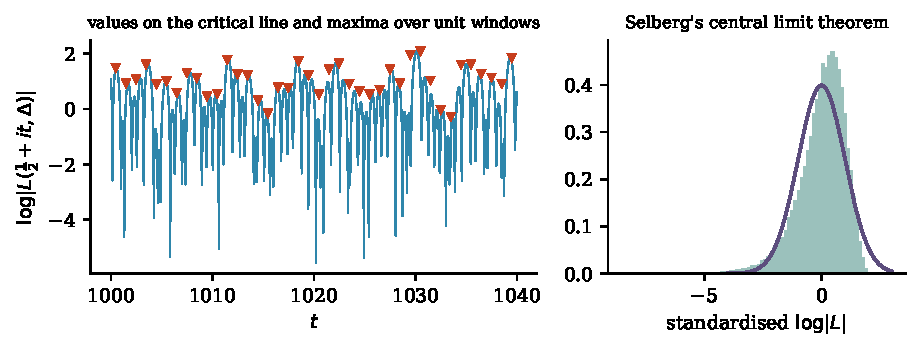
\includegraphics[width=\textwidth]{figs/selberg_clt.pdf}
\caption{Left: $\log|L(6+it,\Delta)|$ for $t\in[1000,1040]$ (the axis label uses the unitary normalisation, with centre $\frac12$), with the maximum over each unit window marked; the downward spikes are zeros. Right: histogram of the standardised values of $\log|L(6+it,\Delta)|$ at $50{,}000$ points of $[500,2500)$ against the standard normal density. The excess on the left is the exponential tail of Proposition~\ref{prop:09blefttail}.}\label{fig:09bclt}
\end{figure}

\subsection{Keating and Snaith, and the hybrid product}\label{sec:09bhybrid}

Keating and Snaith \cite{keatingsnaith2000} modelled $\zeta(\frac12+it)$ near height $T$ by the characteristic polynomial of a Haar random matrix in $\mathrm{U}(N)$ with $N=\log\frac{T}{2\pi}$, the number of zeros in a window of length $2\pi$, and computed its moments exactly.\index{Keating Snaith model}

\begin{proposition}[Keating and Snaith]\label{prop:09bks}
Let $U$ be Haar distributed in $\mathrm{U}(N)$ and $\Lambda_N=\det(I-U)=Z_N(0)$ (Section~\ref{sec:ch6ksnaith}). Then
\begin{align*}
\operatorname{Var}\log|\Lambda_N|&=\frac12\sum_{j=1}^N\psi'(j)=\frac12\Bigl(H_N+N\sum_{k>N}\frac1{k^2}\Bigr)\\
&=\frac12\bigl(\log N+\gamma_{\mathrm E}+1\bigr)+O\bigl(N^{-1}\bigr),
\end{align*}
where $\psi=\Gamma'/\Gamma$, $H_N$ is the harmonic number and $\gamma_{\mathrm E}$ is Euler's constant. For $j\ge3$ the cumulants $\kappa_j(N)$ of $\log|\Lambda_N|$ converge as $N\to\infty$ to
\[
\kappa_j(\infty)=(1-2^{1-j})(-1)^j(j-1)!\,\zeta(j-1);
\]
in particular $\kappa_3(\infty)=-\pi^2/4$ and $\kappa_4(\infty)=\frac{21}{4}\zeta(3)$.
\end{proposition}

\begin{proof}
Keating and Snaith evaluate $\E|\Lambda_N|^s=\prod_{j=1}^N\Gamma(j)\Gamma(j+s)/\Gamma(j+\frac s2)^2$ for $\operatorname{Re}s>-1$ by Selberg's integral \cite{keatingsnaith2000}. The cumulant generating function of $\log|\Lambda_N|$ is therefore
\[
K(s)=\sum_{j\le N}\bigl[\log\Gamma(j)+\log\Gamma(j+s)-2\log\Gamma(j+\tfrac s2)\bigr],
\]
and $\kappa_m=K^{(m)}(0)=(1-2^{1-m})\sum_{j\le N}\psi^{(m-1)}(j)$. For $m=2$ use $\psi'(j)=\sum_{k\ge j}k^{-2}$ and exchange the sums: $\sum_{j\le N}\psi'(j)=\sum_k\min(k,N)k^{-2}=H_N+N\sum_{k>N}k^{-2}$. Since $H_N=\log N+\gamma_{\mathrm E}+O(N^{-1})$ and $N\sum_{k>N}k^{-2}=1+O(N^{-1})$, the variance follows. For $m\ge3$ use $\psi^{(m-1)}(j)=(-1)^m(m-1)!\sum_{k\ge j}k^{-m}$; then $\sum_{j\ge1}\sum_{k\ge j}k^{-m}=\sum_kk^{1-m}=\zeta(m-1)$ converges.
\end{proof}

The random matrix model thus predicts a variance of the right growth, $\frac12\log\log T$, and also a constant, $\frac12(\gamma_{\mathrm E}+1)$. It also predicts that the higher cumulants stay bounded: the non Gaussian features of $\log|\zeta|$ at finite height should be of fixed absolute size, decaying in standard units only like powers of $\log\log T$. For our sample, with variance $1.5265$, the limits $\kappa_3(\infty)$ and $\kappa_4(\infty)$ correspond to skewness $-1.308$ and excess kurtosis $2.708$, against the observed $-1.135$ and $2.493$. The signs and sizes agree; the model is not expected to be exact here, since it ignores the arithmetic.

The arithmetic is restored by the hybrid Euler Hadamard product of Gonek, Hughes and Keating \cite{ghk2007}.\index{hybrid Euler Hadamard product} For a parameter $X\ge2$ they write $\zeta(s)=P_X(s)Z_X(s)$ up to a small error, where $P_X$ is a smoothed Euler product over the primes $p\le X$ and $Z_X$ is a smoothed Hadamard product over the zeros within about $1/\log X$ of $s$. They prove that $\E|P_X|^{2k}\sim a_k(e^{\gamma_{\mathrm E}}\log X)^{k^2}$ as $X,T\to\infty$ with $X=O((\log T)^{2-\varepsilon})$, with the arithmetic factor
\[
a_k=\prod_p\Bigl(1-\frac1p\Bigr)^{k^2}\sum_{m\ge0}\frac{d_k(p^m)^2}{p^m},
\]
conjecture that $\E|Z_X|^{2k}\sim\frac{G(k+1)^2}{G(2k+1)}\bigl(\log T/(e^{\gamma_{\mathrm E}}\log X)\bigr)^{k^2}$, the Keating Snaith moment of a matrix of size $\log T/(e^{\gamma_{\mathrm E}}\log X)$, and conjecture that the two factors are asymptotically independent, so that their moments multiply; they establish both conjectures when $k=1$ and $k=2$. The product recovers the moment conjecture $\E|\zeta|^{2k}\sim a_k\frac{G(k+1)^2}{G(2k+1)}(\log T)^{k^2}$ of Keating and Snaith and of Conrey, Farmer, Keating, Rubinstein and Snaith \cite{cfkrs2005}, and the dependence on $X$ cancels. Here $G$ is Barnes' function and $d_k$ is the $k$ fold divisor function. Reading off the coefficient of $k^2$ in the logarithm of each factor splits the variance into a prime part and a zero part. Since $\log\frac{G(k+1)^2}{G(2k+1)}=(1+\gamma_{\mathrm E})k^2+O(k^3)$ and $d_k(p^m)=k/m+O(k^2)$, the variance implied for $\zeta$ is
\begin{equation}\label{eq:09bvarzeta}
V_\zeta(T)=\frac12\Bigl(\log\log\frac{T}{2\pi}+\gamma_{\mathrm E}+1+A_\zeta\Bigr),\quad A_\zeta=\sum_p\Bigl(\log\Bigl(1-\frac1p\Bigr)+\mathrm{Li}_2\Bigl(\frac1p\Bigr)\Bigr),
\end{equation}
and we computed $A_\zeta=-0.17625$, so that the constant is $\frac12(\gamma_{\mathrm E}+1+A_\zeta)=0.70048$.

For a form of degree two the same recipe gives a conjecture we can test. Write $A_p$ for the Satake parameter of $\Delta$ at $p$, so $\tr A_p^m=2\cos m\theta_p$.

\begin{conjecture}[Variance at finite height; our formulation for $\Delta$]\label{conj:09bvar}
For $t$ uniform on $[T,2T]$,
$\operatorname{Var}\log|L(6+it,\Delta)|=V_\Delta(T)+o(1)$, where
\[
V_\Delta(T)=\frac12\Bigl(\log\Bigl(2\log\frac{T}{2\pi}\Bigr)+\gamma_{\mathrm E}+1+A_\Delta\Bigr)
\]
and
\[
A_\Delta=\sum_p\Bigl(\log\Bigl(1-\frac1p\Bigr)+\sum_{m\ge1}\frac{(2\cos m\theta_p)^2}{m^2p^m}\Bigr).
\]
\end{conjecture}

The term $\log(2\log\frac T{2\pi})$ is $\log N$ for the matrix size $N=2\log\frac{T}{2\pi}$ that matches the doubled density of zeros, and $A_\Delta$ is the coefficient of $k^2$ in the CFKRS arithmetic factor of $\Delta$, obtained exactly as for $\zeta$ from $d_k(\Delta;p^m)=k\tr A_p^m/m+O(k^2)$. The series converges by Lemma~\ref{lem:09brs}, and Exercise~\ref{ex:09bmertens} expresses $A_\Delta$ through $L(1,\Sym^2\Delta)$.

\paragraph{The arithmetic.} From $\tau(p)$ for $p\le10^5$ we find $A_\Delta=-0.898$: the partial sums are $-0.8946$, $-0.8966$, $-0.8976$ at $p\le2500$, $10^4$, $10^5$, and the identity of Exercise~\ref{ex:09bmertens} gives the limit $-0.8979$. Below we use the value $-0.8976$. At $T=1500$ the five pieces of $V_\Delta$ are
\[
\underbrace{\tfrac12\log\log T}_{0.9948}+\underbrace{\tfrac12\log2}_{0.3466}+\underbrace{\tfrac12\log\frac{\log(T/2\pi)}{\log T}}_{-0.1447}+\underbrace{\tfrac12(\gamma_{\mathrm E}+1)}_{0.7886}+\underbrace{\tfrac12A_\Delta}_{-0.4488}=1.5365 .
\]
Our sample is spread over $t\in[500,2500]$, and the average of $V_\Delta(t)$ over that range is $1.5268$, against the observed variance $1.5265$. The leading term $\frac12\log\log t$ accounts for only $65$ per cent of the observed variance. The random matrix constant without the arithmetic factor, $\frac12(\log(2\log\frac{t}{2\pi})+\gamma_{\mathrm E}+1)$, averages $1.9756$ and overshoots by $0.45$. The prime model alone, the variance of the random Euler product with the true Satake angles at the primes $p\le t$, gives $0.76$, $0.81$, $0.84$, $0.87$ at $t=500$, $1000$, $1500$, $2500$, and undershoots by about $0.7$; its deficit against $\frac12\log\log t$ comes from the negative constant $B_\Delta$ of Lemma~\ref{lem:09brs}, partly offset by the prime powers. Only the combination of Conjecture~\ref{conj:09bvar} accounts for the data, and it does so within the sampling error. The $50{,}000$ values are strongly dependent, but batch means, a moving block bootstrap and a Bartlett long run variance, with blocks or bandwidths of $1$ to $100$ units of $t$, put the standard error of the sample variance between $0.012$ and $0.018$, far below the distance of $0.45$ or more from each of the three alternatives above. Corrections of relative order $1/\log t$ are also expected. The agreement to the third decimal is therefore luck; the agreement within the sampling error, over a single range of heights, is evidence for the conjecture, not a test of its error term. The split of $V_\Delta$ into a prime part and a zero part is not unique, and the moment theorem of Gonek, Hughes and Keating concerns $X=O((\log T)^{2-\varepsilon})$, not $X=T$; what is tested is the combination $V_\Delta$, in which $X$ does not appear.

\section{A log correlated field}\label{sec:09blogcorr}

\subsection{Covariance across scales}

The variance $\frac12\log\log T$ is the sum of contributions $\frac1{2p}$ from the primes, and the dependence between nearby points is decided prime by prime. The following proposition makes this exact for the random model.\index{log correlated field}

\begin{proposition}[Covariance of the random model; this book]\label{prop:09bcov}
Let $(U_p)$ be independent and uniform on the unit circle, and for $P\ge3$ and real $h$ put $X_P(h)=\operatorname{Re}\sum_{p\le P}U_pp^{-1/2-ih}$. Then
\begin{align*}
\operatorname{Cov}\bigl(X_P(h),X_P(h')\bigr)&=\frac12\sum_{p\le P}\frac{\cos\bigl((h-h')\log p\bigr)}{p}\\
&=\frac12\log\min\Bigl(\log P,\frac{1}{|h-h'|}\Bigr)+O(1),
\end{align*}
uniformly in $P$ and in $0<|h-h'|\le1$. The same holds for the field $X^\Delta_P(h)=\operatorname{Re}\sum_{p\le P}\lambda(p)U_pp^{-1/2-ih}$, with $\lambda(p)^2/p$ in place of $1/p$ in the sum.
\end{proposition}

\begin{proof}
For independent uniform $U$, $\E\operatorname{Re}(Ua)\operatorname{Re}(Ub)=\frac12\operatorname{Re}(a\bar b)$, which gives the first identity. Put $u=|h-h'|$ and $Q=\min(P,e^{1/u})$. For $p\le Q$ we have $\cos(u\log p)=1+O(u^2\log^2p)$, and $\sum_{p\le Q}u^2\log^2p/p\ll u^2\log^2Q\le1$ by Mertens' estimate $\sum_{p\le y}\log p/p=\log y+O(1)$ and partial summation. So the primes $p\le Q$ contribute $\frac12\sum_{p\le Q}1/p+O(1)=\frac12\log\log Q+O(1)$. If $P>e^{1/u}$ the remaining primes contribute $\frac12\sum_{e^{1/u}<p\le P}\cos(u\log p)/p$. By the prime number theorem with remainder $O(y/\log^2y)$ and partial summation, this equals $\frac12\int_{1/u}^{\log P}\cos(uv)\,\frac{dv}{v}+O(u)$, and the integral is $\int_1^{u\log P}\cos w\,\frac{dw}{w}$, which is bounded uniformly. Since $\log\log Q=\log\min(\log P,1/u)$, the formula follows. For $X^\Delta_P$ the same argument applies with Lemma~\ref{lem:09brs} and the prime number theorem for $L(s,\Delta\times\Delta)=\zeta(s)L(s,\Sym^2\Delta)$ in the form $\sum_{p\le y}\lambda(p)^2\log p=y+O(y/\log^2y)$, which follows from the zero free regions used in the proof of the lemma, in place of Mertens and the prime number theorem.
\end{proof}

At $h=h'$ the variance is $\frac12\log\log P+O(1)$. Two points at distance $u$ are almost perfectly correlated in the primes up to $e^{1/u}$ and almost uncorrelated beyond, so for $1/\log P\le u\le1$ the correlation coefficient is $\log(1/u)/\log\log P+O(1/\log\log P)$. This is the defining property of a log correlated field. For $\zeta$ itself the analogous statement is a theorem of Bourgade \cite{bourgade2010}: for shifts $h_1,\dots,h_k$ with $|h_i-h_j|=(\log T)^{-c_{ij}+o(1)}$, $0\le c_{ij}\le1$, the vector $(\log\zeta(\frac12+i(t+h_j)))_j/\sqrt{\frac12\log\log T}$ is asymptotically complex Gaussian, with correlation $c_{ij}$ between the real parts. Thus, to leading order, the covariance of $\log|\zeta|$ at distance $u$ is $\frac12\log(1/u)$ for $1/\log T\le u\le1$, saturating at $\frac12\log\log T$ below the scale $1/\log T$ of the zero spacings.

\subsection{The branching picture}

Group the primes into blocks $e^{e^{k-1}}<p\le e^{e^k}$, $k=1,\dots,n$ with $n=\log\log T$, and write the field of Proposition~\ref{prop:09bcov} with $P=T$ as $X_T(h)=\sum_kY_k(h)$, with $Y_k$ the contribution of block $k$. Each block has variance about $\frac12$, since $\sum1/p$ over a block is about $1$. Inside a window $|h|\le1$, $Y_k$ is essentially constant on intervals of length $e^{-k}$ and essentially independent across such intervals, because its frequencies $\log p$ are about $e^k$. So $X_T$ restricted to the window is approximately a branching random walk: a tree in which every vertex at level $k$ has about $e$ children, each level adds an independent Gaussian increment of variance $\frac12$, and the leaves at level $n$ are the effectively distinct values of the field, about $e^n=\log T$ per unit length, one for each interval of length $1/\log T$, the scale of the zero spacings.\index{branching random walk} Figure~\ref{fig:09bfield} shows the picture for the field
\[
R_X(t)=\sum_{p\le X}\frac{2\cos\theta_p\cos(t\log p)}{\sqrt p}=\operatorname{Re}\sum_{p\le X}2\cos\theta_p\,p^{-1/2-it},
\]
the prime part of $\log|L_{\mathrm{rand}}(\frac12+it)|$ for the Sato Tate random Euler product of Chapter~\ref{ch:09}, with $\theta_p$ independent with the Sato Tate law, built up through the levels $X=e^{e^{k/2}}$, $k=1,\dots,5$ (that is $5.2$, $15.2$, $88.4$, $1618$, $195339$), and then $X=10^6$.

\begin{figure}[t]\centering
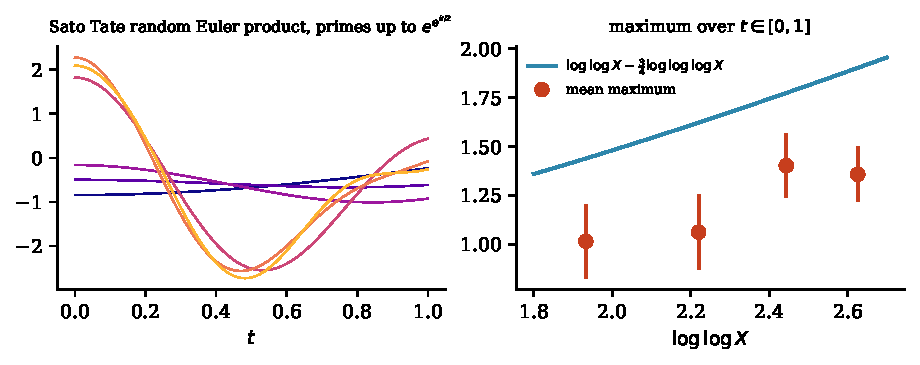
\includegraphics[width=\textwidth]{figs/random_field.pdf}
\caption{Left: one realisation of the field $R_X(t)=\sum_{p\le X}2\cos\theta_p\cos(t\log p)/\sqrt p$ of the Sato Tate random Euler product on $t\in[0,1]$, built up by adding the primes in successive ranges $p\le e^{e^{k/2}}$, $k=1,\dots,5$, and then $p\le10^6$; each level refines the previous one on a finer scale, which is the branching structure. Right: mean of $\max_{t\in[0,1]}R_X(t)$ for $X=10^3,10^4,10^5,10^6$ ($300$, $200$, $80$ and $30$ draws) against the curve $\log\log X-\frac34\log\log\log X$. The error bars are one standard deviation divided by $\sqrt{30}$ at every point, which overstates the standard error of the first three means. The offset is an additive constant that the theory does not determine.}\label{fig:09bfield}
\end{figure}

The maximum of a branching random walk is understood in detail, and it is the source of the constant $\frac34$. We isolate the computation in a continuous model where it can be done exactly. Let $b\ge2$ be an integer, $\sigma>0$, and let $\{B_v(s):0\le s\le n\}$, indexed by the $b^n$ leaves $v$ of the $b$ ary tree of depth $n$, be Brownian motion indexed by the tree: each edge carries an independent Brownian path of duration one and variance $\sigma^2$ per unit time, and $B_v$ is the concatenation along the path from the root to $v$. At integer times this is a branching random walk with $N(0,\sigma^2)$ increments. Put
\[
c=\sigma\sqrt{2\log b},\qquad\theta=\frac{c}{\sigma^2}=\frac{\sqrt{2\log b}}{\sigma},\qquad x_n=cn-a\log n
\]
for a constant $a>0$.

\begin{proposition}[First moments with and without the ballot constraint; this book]\label{prop:09bballot}
Fix $y\ge0$. Let $N_n(y)$ be the number of leaves with $B_v(n)\ge x_n+y$, and $Z_n(y)$ the number of leaves with $B_v(n)\in[x_n+y,x_n+y+1]$ and $B_v(s)\le\frac snx_n+y+1$ for all $s\in[0,n]$. As $n\to\infty$,
\[
\E N_n(y)\sim\frac{\sigma}{c\sqrt{2\pi}}\,n^{\theta a-\frac12}e^{-\theta y},\qquad
\E Z_n(y)\sim\kappa\,(1+y)\,n^{\theta a-\frac32}e^{-\theta y},
\]
with $\kappa=2(\theta-1+e^{-\theta})/(\sigma^3\theta^2\sqrt{2\pi})$.
In particular the choice $a=\frac1{2\theta}$ makes $\E N_n$ of order one, while $a=\frac3{2\theta}$ makes $\E Z_n(y)\to\kappa(1+y)e^{-\theta y}$, and for that choice $\E N_n(y)$ grows like $n$.
\end{proposition}

\begin{proof}
Each $B_v(n)$ is $N(0,\sigma^2n)$ with density $\varphi_n$. For $z=x_n+y+u$ with $u$ bounded,
\begin{align*}
\frac{z^2}{2\sigma^2n}&=\frac{c^2n}{2\sigma^2}-\frac{c}{\sigma^2}(a\log n-y-u)+O\Bigl(\frac{\log^2n}{n}\Bigr)\\
&=n\log b-\theta a\log n+\theta(y+u)+o(1),
\end{align*}
so $b^n\varphi_n(z)=(\sigma\sqrt{2\pi n})^{-1}n^{\theta a}e^{-\theta(y+u)}(1+o(1))$. The first claim follows from $\E N_n(y)=b^n\Prob(B(n)\ge x_n+y)$ and the Mills ratio $\Prob(B(n)\ge z)\sim\sigma^2n\,\varphi_n(z)/z$ with $z\sim cn$. For the second, condition on $B_v(n)=x_n+y+u$, $u\in[0,1]$. The process $R(s)=B_v(s)-\frac snx_n$ is then a Brownian bridge of variance $\sigma^2$ per unit time from $0$ to $y+u$ on $[0,n]$, and the constraint is $R\le y+1$. By the reflection principle a bridge from $0$ to $e$ of duration $n$ stays below a level $h>\max(0,e)$ with probability $1-\exp(-2h(h-e)/(\sigma^2n))$. With $h=y+1$ and $e=y+u$ this is $\frac{2(1+y)(1-u)}{\sigma^2n}(1+o(1))$. Integrating against $b^n\varphi_n(x_n+y+u)\,du$ over $[0,1]$ gives
\[
\E Z_n(y)\sim\frac{2(1+y)}{\sigma^3\sqrt{2\pi}}\,n^{\theta a-\frac32}e^{-\theta y}\int_0^1(1-u)e^{-\theta u}\,du,
\]
and $\int_0^1(1-u)e^{-\theta u}du=(\theta-1+e^{-\theta})/\theta^2$.
\end{proof}

The proposition explains the two corrections. The naive first moment places the maximum at $cn-\frac1{2\theta}\log n$. But the leaves that reach that height are overwhelmingly descendants of ancestors that were already too high at intermediate levels, and such ancestors are rare; they occur with probability tending to zero, while each of them produces a large number of high leaves, which is how the expectation can be large while the typical count is zero. Requiring the path to stay below the straight line to its endpoint, a ballot constraint, costs a factor $1/n$, and this moves the correct centring to $m_n=cn-\frac{3}{2\theta}\log n$. The factor $1+y$ is the ballot probability for a path that starts at distance $y+1$ below the barrier, and it produces a right tail of the form $ye^{-\theta y}$ for the maximum. That the constrained first moment gives the right answer is the content of the following theorem.

\begin{theorem}[Bramson; Addario Berry and Reed; A\"id\'ekon]\label{thm:09bbrw}
For the branching random walk above, with $M_n=\max_vB_v(n)$ and $m_n=cn-\frac{3}{2\theta}\log n$, the sequence $M_n-m_n$ is tight, and it converges in law: there are a constant $C^*>0$ and a positive random variable $D_\infty$, the limit of the derivative martingale, such that
\[
\Prob(M_n\le m_n+y)\longrightarrow\E\bigl[\exp\bigl(-C^*D_\infty e^{-\theta y}\bigr)\bigr]\qquad(y\in\R).
\]
\end{theorem}

The limit is a Gumbel law randomly shifted by $\theta^{-1}\log(C^*D_\infty)$. Bramson \cite{bramson1978} proved the $\frac{3}{2\theta}\log n$ correction for branching Brownian motion, where Lalley and Sellke \cite{lalleysellke1987} identified the derivative martingale; Addario Berry and Reed \cite{addarioberryreed2009} proved tightness for branching random walks, and A\"id\'ekon \cite{aidekon2013} the convergence in law. The book of Bovier \cite{bovier2017} and the lecture notes of Kistler \cite{kistler2015} explain the method, whose heart is a refinement of Proposition~\ref{prop:09bballot}.

For the zeta field the parameters are fixed by the variance and the number of leaves. Take $b=2$ and $n_2=\lfloor\log\log T/\log2\rfloor$ levels of variance $\sigma^2=\frac12\log2$, so that a leaf has variance $\frac12\log\log T$ and there are $2^{n_2}\approx\log T$ leaves. Then $c=\log2$ and $\theta=2$, so $cn_2=\log\log T+O(1)$, $\frac3{2\theta}\log n_2=\frac34\log\log\log T+O(1)$, and the right tail is $ye^{-2y}$. The value $\theta=2$ does not depend on the choice of tree: per unit of $\log\log T$ the field gains variance $\frac12$ while the number of leaves is multiplied by $e$, so the speed is $c=1$ per unit and $\theta=c/\sigma^2=2$.

\subsection{The Fyodorov Hiary Keating conjecture}

\begin{conjecture}[Fyodorov, Hiary and Keating \cite{fhk2012,fyodorovkeating2014}]\label{conj:09bfhk}\index{Fyodorov Hiary Keating conjecture}
Let $\tau$ be uniform on $[T,2T]$. Then
\[
\max_{|h|\le1}\log\bigl|\zeta\bigl(\tfrac12+i(\tau+h)\bigr)\bigr|=\log\log T-\tfrac34\log\log\log T+\mathcal{M}_T,
\]
where $\mathcal{M}_T$ converges in law to a random variable $\mathcal{M}$ with $\Prob(\mathcal{M}>y)\sim Cye^{-2y}$ as $y\to\infty$.
\end{conjecture}

Fyodorov, Hiary and Keating reached the conjecture through random matrix theory, predicting by a freezing transition that $\max_\phi\log|\det(I-Ue^{-i\phi})|=\log N-\frac34\log\log N+O(1)$ for Haar unitary $U$, and matching $N=\log T$. For the matrices they also predicted the law of the bounded term, and they compared their predictions with Hiary's computations of $\zeta$ at large height. The tail $ye^{-2y}$ is expected to carry over to $\zeta$, but the law itself is not expected to coincide with the random matrix one \cite{fyodorovkeating2014,abr2023}. The branching random walk gives the same centring.

What is proved is the following.

\begin{theorem}\label{thm:09bfhkproved}
Let $\tau$ be uniform on $[T,2T]$, and write
\[
M_T=\max_{|h|\le1}\log\bigl|\zeta\bigl(\tfrac12+i(\tau+h)\bigr)\bigr|,\qquad m_T=\log\log T-\tfrac34\log\log\log T .
\]
\begin{enumerate}
\item (First order.) For every $\varepsilon>0$, with probability tending to one, $|M_T-\log\log T|\le\varepsilon\log\log T$. This is due to Najnudel \cite{najnudel2018}, assuming the Riemann hypothesis, and to Arguin, Belius, Bourgade, Radziwi\l\l\ and Soundararajan \cite{abbrs2019} unconditionally.
\item (Upper tail.) Arguin, Bourgade and Radziwi\l\l\ \cite{abr2020} prove that $\Prob(M_T>m_T+y)\ll ye^{-2y}$ for all large $T$, uniformly in $y\ge1$; in particular $M_T-m_T$ is bounded above in probability.
\item (Lower bounds.) In a second paper \cite{abr2023} the same authors prove that $\Prob(M_T<m_T-y)\to0$ as $y\to\infty$, uniformly in large $T$, and that $\Prob(M_T>m_T+y)\gg ye^{-2y}$ for $10\le y\le\sqrt{\log\log T}$. Together the two papers show that $M_T-m_T$ is tight, with right tail of exact order $ye^{-2y}$ in that range.
\end{enumerate}
\end{theorem}

Before the work of Arguin, Bourgade and Radziwi\l\l, Harper \cite{harper2019} proved that with probability tending to one
\[
\max_{|h|\le1/2}\log\bigl|\zeta\bigl(\tfrac12+i(\tau+h)\bigr)\bigr|\le\log\log T-\bigl(\tfrac34+o(1)\bigr)\log\log\log T,
\]
the first upper bound with the correct second term, by bounding the critical partition function $\int_{|h|\le1/2}|\zeta(\frac12+i(\tau+h))|^2dh$. What remains open is the convergence in law of $\mathcal{M}_T$ (tightness gives only subsequential limits), the tail constant $C$, and the form of the limit, which by analogy with Theorem~\ref{thm:09bbrw} and with the random matrix case one expects to be a randomly shifted Gumbel law. For random unitary matrices more is known: the leading order is due to Arguin, Belius and Bourgade \cite{abb2017}, the second order term $-\frac34\log\log N$ to Paquette and Zeitouni \cite{paquettezeitouni2018}, tightness at the scale $\log N-\frac34\log\log N$ to Chhaibi, Madaule and Najnudel \cite{cmn2018}, and Paquette and Zeitouni \cite{paquettezeitouni2022} proved, for the circular $\beta$ ensembles, convergence in law to the sum of a Gumbel variable and an independent variable defined through a derivative martingale.

For a degree two form the Rankin Selberg variance and the doubled density of zeros change only $O(1)$ terms in the heuristic: the leaves are the $2\log T$ effectively distinct values per unit window, and $\log\log(T^2)=\log\log T+\log2$. We therefore expect $\max_{|h|\le1}\log|L(6+i(\tau+h),\Delta)|=\log\log T-\frac34\log\log\log T+O_{\Prob}(1)$, with an additive constant that differs from that of $\zeta$. We are not aware of a proof for $\Delta$, even to first order, though we expect the methods of \cite{abbrs2019} to extend.

\paragraph{Data.} We split $[500,2500]$ into $2000$ unit windows and recorded the maximum of $\log|L(6+it,\Delta)|$ in each (Figure~\ref{fig:09bclt}, left). The mean of the window maxima is $1.1010$ with standard deviation $0.5674$, and the mean of $\log\log t-\frac34\log\log\log t$ at the window centres is $1.4655$. The difference has mean $-0.3645$ and standard deviation $0.5657$, so the standard error of the mean difference is about $0.013$ (the windows are adjacent, so slightly more in truth). This is consistent with a bounded additive correction, which neither the conjecture nor the theorem determines. It is not evidence for the $\frac34$: over $[500,2500]$ the term $\frac34\log\log\log t$ varies only between $0.45$ and $0.54$, so it cannot be separated from an unknown constant. For the field $R_X$ of Figure~\ref{fig:09bfield} the mean maxima over $t\in[0,1]$ are $1.015$, $1.062$, $1.402$, $1.358$ for $X=10^3,10^4,10^5,10^6$, from $300$, $200$, $80$ and $30$ draws with standard deviations $1.03$, $1.05$, $0.89$, $0.77$, against $\log\log X-\frac34\log\log\log X=1.438$, $1.622$, $1.773$, $1.902$. The differences, $-0.42$, $-0.56$, $-0.37$, $-0.54$, with standard errors $0.06$, $0.07$, $0.10$, $0.14$, are consistent with a constant offset (weighted mean $-0.47$, $\chi^2=3.3$ on $3$ degrees of freedom), and the decrease of the mean maximum from $10^5$ to $10^6$ is within noise; the range of $X$ is too short to separate the $\frac34\log\log\log X$ term from the constant. The model is also not stationary: $\E R_X(t)^2=\frac12\sum_{p\le X}(1+\cos(2t\log p))/p$ is close to $\log\log X$ rather than $\frac12\log\log X$ near $t=0$, so we use it only to show the branching mechanism.

\section{Multiplicative chaos}\label{sec:09bchaos}

Exponentiating a log correlated field produces a random measure. Let $Y$ be a centred Gaussian field on an interval with $\E Y(x)Y(x')=\log\frac{1}{|x-x'|}+g(x,x')$, $g$ bounded and continuous. The field is not defined pointwise, but its regularisations $Y_\varepsilon$ at scale $\varepsilon$ are, and Kahane \cite{kahane1985} showed that, for suitable regularisations and $0<\gamma<\sqrt2$, the measures
\[
M_{\gamma,\varepsilon}(dx)=e^{\gamma Y_\varepsilon(x)-\frac{\gamma^2}2\E Y_\varepsilon(x)^2}\,dx
\]
converge, as $\varepsilon\to0$, to a nontrivial random measure $M_\gamma$, the \emph{Gaussian multiplicative chaos}\index{multiplicative chaos} of parameter $\gamma$; later work showed that the limit does not depend on the regularisation \cite{rhodesvargas2014}, and it is carried by a set of points where $Y$ is atypically large, of dimension $1-\gamma^2/2$. For $\gamma\ge\sqrt2$ the normalised measures tend to zero. At the critical value $\gamma=\sqrt2$ a nontrivial limit is obtained either from the derivative martingale or by the Seneta Heyde normalisation $\sqrt{\log(1/\varepsilon)}\,M_{\sqrt2,\varepsilon}$, and the two constructions agree up to a constant factor, as shown by Duplantier, Rhodes, Sheffield and Vargas \cite{dsrv2014,dsrv2014b}. The survey of Rhodes and Vargas \cite{rhodesvargas2014} gives the theory.

The dictionary with $\zeta$ follows from Proposition~\ref{prop:09bcov}. The field $\log|\zeta(\frac12+i(\tau+x))|$ has covariance $\frac12\log\frac1{|x-x'|}$ down to the scale $\varepsilon=1/\log T$, so $Y=\sqrt2\log|\zeta|$ is normalised as above, and
\[
|\zeta|^{2\beta}=e^{2\beta\log|\zeta|}=e^{\sqrt2\beta Y}:\qquad\gamma=\sqrt2\,\beta .
\]
The measures $|\zeta(\frac12+i(\tau+x))|^{2\beta}dx$, normalised by their mean $(\log T)^{\beta^2}$ up to constants, are therefore expected to converge to subcritical chaos for $\beta<1$, and $\beta=1$, the measure $|\zeta|^2dx$ whose mean is the classical Hardy Littlewood second moment, is exactly critical. The critical measure carries the information about the maximum. Its Seneta Heyde factor $\sqrt{\log\log T}$ is the inverse of the probability, of order $1/\sqrt n$ with $n=\log\log T$ levels, that a random walk stays below a barrier; Proposition~\ref{prop:09bballot} computes the same constraint for a bridge, whose cost is $1/n$.

Saksman and Webb proved a statement of this kind for $\zeta$ itself rather than for powers of its modulus.

\begin{theorem}[Saksman and Webb \cite{saksmanwebb2020}]\label{thm:09bsw}
Let $\omega$ be uniform on $[0,1]$. As $T\to\infty$, the random generalised function $x\mapsto\zeta(\frac12+ix+i\omega T)$ on a fixed bounded interval converges in law, in the Sobolev space $W^{-\alpha,2}$ for any $\alpha>\frac12$, to the random generalised function
\[
\zeta_{\mathrm{rand}}(\tfrac12+ix)=\lim_{N\to\infty}\prod_{p\le N}\bigl(1-U_pp^{-1/2-ix}\bigr)^{-1},
\]
with $(U_p)$ independent and uniform on the unit circle, the limit taken in the same space. Moreover $\zeta_{\mathrm{rand}}(\frac12+ix)$ is the product of a random smooth function and a complex Gaussian multiplicative chaos, the exponential of a complex Gaussian field whose real and imaginary parts are log correlated.
\end{theorem}

No normalisation is needed: the shifted zeta function itself has a limit, but only as a generalised function. The chaos is complex: the exponent $\sum_pU_pp^{-1/2-ix}$ has real and imaginary parts, each with covariance $\frac12\log\frac1{|x-x'|}+O(1)$. Saksman and Webb formulate the convergence of $|\zeta|^{2\beta}dx$ to subcritical chaos for $\beta<1$ as a conjecture, together with the critical case: that
\[
\sqrt{\log\log T}\,(\log T)^{-1}\bigl|\zeta\bigl(\tfrac12+ix+i\omega T\bigr)\bigr|^2dx
\]
converges in law to a constant multiple of a critical chaos measure. Both conjectures are open in print as we write; Gorodetsky and Wong \cite{gorodetskywong2025} report that the critical one will be established in forthcoming work of Harper, Saksman and Webb. For the truncated random Euler product the analogous critical statement is a theorem of Saksman and Webb.

Figure~\ref{fig:09bchaos} shows, for a single realisation, the squared modulus of the random Euler product $\prod_{p\le N}(1-U_pp^{-1/2-it})^{-1}$ truncated at $N=2\times10^5$, on a logarithmic scale. The measure is concentrated in thin spikes separated by long stretches where it is small. This is the behaviour expected near criticality: for $\gamma<\sqrt2$ the chaos is carried by a set of dimension $1-\gamma^2/2$, which shrinks to dimension zero at the critical value.

\begin{figure}[t]\centering
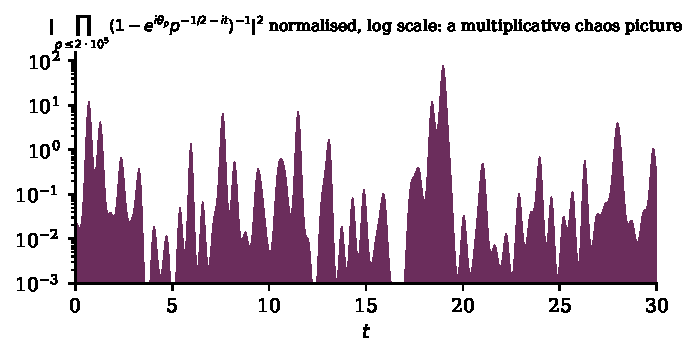
\includegraphics[width=\textwidth]{figs/chaos.pdf}
\caption{One realisation of $|\prod_{p\le2\cdot10^5}(1-U_pp^{-1/2-it})^{-1}|^2$ for $t\in[0,30]$, with $U_p$ independent and uniform on the unit circle (the Steinhaus random Euler product), divided by its mean over the window, on a logarithmic scale. The mass sits on a sparse set of spikes: a picture of critical multiplicative chaos ($\beta=1$, $\gamma=\sqrt2$), cut off at the scale $1/\log(2\cdot10^5)$.}\label{fig:09bchaos}
\end{figure}

\paragraph{Moments of moments.} The freezing transition behind Conjecture~\ref{conj:09bfhk} is visible in the moments of the chaos. For $U$ Haar in $\mathrm{U}(N)$ and $Z_N(\phi)=\det(I-Ue^{-i\phi})$, Fyodorov and Keating \cite{fyodorovkeating2014} studied
\[
\mathrm{MoM}_N(k,\beta)=\E\Bigl[\Bigl(\frac1{2\pi}\int_0^{2\pi}|Z_N(\phi)|^{2\beta}d\phi\Bigr)^k\Bigr]
\]
and conjectured that it grows like $N^{k\beta^2}$ when $k\beta^2<1$ and like $N^{k^2\beta^2-k+1}$ when $k\beta^2>1$. Below the transition the $k$th moment of the total mass of the limiting chaos is finite, and $\mathrm{MoM}_N$ is of the order of the $k$th power of the mean; above it, the moment is dominated by the neighbourhood of the maximum. Bailey and Keating \cite{baileykeating2019} proved that for positive integers $k$ and $\beta$, $\mathrm{MoM}_N(k,\beta)$ is a polynomial in $N$ of degree $k^2\beta^2-k+1$, confirming the exponent in the second regime for integer parameters. Relatedly, Arguin, Belius and Bourgade \cite{abb2017} proved that the free energy $\frac1{\log N}\log\frac1{2\pi}\int_0^{2\pi}|Z_N(\phi)|^{2\beta}d\phi$ converges in probability to $\beta^2$ for $\beta\le1$ and to $2\beta-1$ for $\beta\ge1$, the slope $2$ above the transition reflecting a maximum of $\log|Z_N|$ equal to $\log N$ to first order.

\section{Random multiplicative functions}\label{sec:09bharper}

The random Euler product has a Dirichlet series, and its coefficients are a random multiplicative function. In the \emph{Steinhaus model} $f(p)=U_p$ are independent and uniform on the unit circle and $f$ is completely multiplicative; in the \emph{Rademacher model} of Wintner \cite{wintner1944} $f(p)=\pm1$ with independent fair signs and $f$ is supported on squarefree integers. Write $S(x)=\sum_{n\le x}f(n)$.\index{random multiplicative function}

For the Steinhaus model $\E f(n)\overline{f(m)}=\mathbb{I}_{n=m}$ by unique factorisation, so $\E|S(x)|^2=\lfloor x\rfloor$. If $S(x)/\sqrt x$ were approximately a standard complex Gaussian, we would have $\E|S(x)|\sim\frac{\sqrt\pi}{2}\sqrt x=0.886\sqrt x$. Helson \cite{helson2010} conjectured instead that $\E|S(x)|=o(\sqrt x)$, and Harper proved it with the exact rate.

\begin{theorem}[Harper \cite{harper2020}]\label{thm:09bharper}\index{Harper's theorem}
Let $f$ be a Steinhaus random multiplicative function. Uniformly for all large $x$ and $0\le q\le1$,
\[
\E|S(x)|^{2q}\asymp\Bigl(\frac{x}{1+(1-q)\sqrt{\log\log x}}\Bigr)^q .
\]
In particular $\E|S(x)|$ is of exact order $\sqrt x\,(\log\log x)^{-1/4}$. The same bounds hold for the Rademacher model.
\end{theorem}

Harper calls this better than square root cancellation. The mechanism is critical multiplicative chaos, and it can be seen through an exact identity.

\begin{lemma}[Plancherel identity]\label{lem:09bplancherel}
Let $f$ be any function on the positive integers with $|f|\le1$, $S(u)=\sum_{n\le u}f(n)$ and $F(s)=\sum_nf(n)n^{-s}$. For $\sigma>1$,
\[
\int_1^\infty\frac{|S(u)|^2}{u^{1+2\sigma}}\,du=\frac{1}{2\pi}\int_{-\infty}^\infty\frac{|F(\sigma+it)|^2}{|\sigma+it|^2}\,dt .
\]
\end{lemma}

\begin{proof}
By partial summation $F(s)=s\int_1^\infty S(u)u^{-s-1}du$ for $\operatorname{Re}s>1$. Put $g(v)=S(e^v)e^{-\sigma v}$ for $v\ge0$ and $g=0$ for $v<0$; then $g\in L^1\cap L^2$ since $|S(u)|\le u$ and $\sigma>1$, and its Fourier transform is $\int_0^\infty S(e^v)e^{-(\sigma+it)v}dv=F(\sigma+it)/(\sigma+it)$. Plancherel's theorem and the substitution $u=e^v$ give the identity.
\end{proof}

For the Steinhaus model the identity continues to hold almost surely for $\sigma>\frac12$, by the same argument once one knows that $S(u)\ll u^{1/2+\varepsilon}$ almost surely, which follows from the method Wintner used for the Rademacher model. Harper works at $\sigma=\frac12+1/\log x$, where the left side is a weighted average of $|S(u)|^2/u$ over $u$ up to about $x$, on a logarithmic scale, and the right side is, up to the factor $\frac1{2\pi}$, the total mass of the measure $|F(\frac12+\frac1{\log x}+it)|^2dt/|\frac12+it|^2$. Since $\log|F(\frac12+\frac1{\log x}+it)|$ is approximately the log correlated field of Proposition~\ref{prop:09bcov} with $P=x$, this is a critical chaos measure, cut off at scale $1/\log x$. Its expectation is of order $\log x$, but its typical size is of order $\log x/\sqrt{\log\log x}$, the Seneta Heyde factor again. Conditionally on the values $f(p)$ for the small primes, $S(x)$ is roughly Gaussian with variance of the order of $\frac{x}{\log x}$ times the total mass, so that
\[
\E|S(x)|\approx\sqrt{\frac{x}{\log x}}\cdot\sqrt{\frac{\log x}{\sqrt{\log\log x}}}=\frac{\sqrt x}{(\log\log x)^{1/4}} .
\]
Harper's proof turns each step of this heuristic into an inequality, and the hard step is the upper bound for low moments of the critical chaos mass, which he proves with a barrier argument of ballot type for the random walk formed by the logarithms of the partial Euler products.

\paragraph{Data.} We drew $400$ Steinhaus functions and computed $S(x)$ for $x\le10^6$. The estimates of $\E|S(x)|/\sqrt x$ at $x=10^3,3\cdot10^3,10^4,3\cdot10^4,10^5,3\cdot10^5,10^6$ are $0.773$, $0.765$, $0.807$, $0.798$, $0.778$, $0.777$, $0.781$, and their ratios to $(\log\log x)^{-1/4}$ are $0.91$, $0.92$, $0.98$, $0.99$, $0.97$, $0.98$, $0.99$ (Figure~\ref{fig:09bharper}). Since $\E|S(x)|^2=\lfloor x\rfloor$, the standard deviation of $|S(x)|/\sqrt x$ is about $\sqrt{1-0.78^2}\approx0.63$, so each estimate has a standard error of about $0.03$; the estimates at different $x$ come from the same $400$ functions and are correlated. Every estimate lies between two and a half and four standard errors below the Gaussian value $0.886$, which is the qualitative content of the theorem. The rate is another matter: over this range $(\log\log x)^{-1/4}$ falls only from $0.848$ to $0.786$, about two standard errors, and the estimates do not decrease monotonically, so the data are consistent with the theorem but cannot confirm the exponent $\frac14$. Gorodetsky and Wong \cite{gorodetskywong2025} have since proved that $(\log\log x)^{1/4}S(x)/\sqrt x$ converges in distribution, answering a question of Harper; since Theorem~\ref{thm:09bharper} with $q=\frac34$ makes these variables uniformly integrable, $c(x)=\E|S(x)|(\log\log x)^{1/4}/\sqrt x$ converges too. We know of no closed form for the limit, and our ratios are only rough estimates of it (Computational Problem~\ref{cp:09bharper}).

\begin{figure}[t]\centering
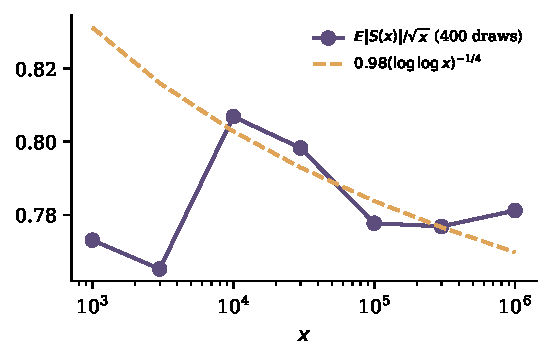
\includegraphics[width=0.62\textwidth]{figs/harper.pdf}
\caption{Estimates of $\E|S(x)|/\sqrt x$ for the Steinhaus random multiplicative function from $400$ draws (standard error about $0.03$ per point), against $0.98(\log\log x)^{-1/4}$: the rate of Theorem~\ref{thm:09bharper}, with the constant $0.98$ chosen to match the data, since the theorem gives none. A complex Gaussian with the same second moment would give $0.886$.}\label{fig:09bharper}
\end{figure}

\paragraph{Deterministic consequences.} Harper transferred the mechanism to deterministic families. For a large prime $r$ and Dirichlet characters $\chi$ modulo $r$, the sums $\sum_{n\le x}\chi(n)$ have mean square $x$ over $\chi$ when $x<r$, by orthogonality; Harper \cite{harper2023} showed that their first absolute moment is $O(\sqrt x/(\log\log(10L))^{1/4})$ with $L=\min(x,r/x)$, hence $o(\sqrt x)$ whenever $x\to\infty$ and $r/x\to\infty$, and proved the analogous statement for zeta sums $\sum_{n\le x}n^{it}$ with $t$ uniform on $[0,T]$ and $L=\min(x,T/x)$. Averaging over characters makes the $\chi(p)$ behave like the Steinhaus $f(p)$ to the extent needed. Sharp bounds for higher moments of random multiplicative functions, where Gaussian heuristics fail in the opposite direction, are in the companion paper of Harper \cite{harper2019b}.

\section{Pair correlation of the zeros of $L(s,\Delta)$}\label{sec:09bpair}

Up to a smooth term, $\log|L|$ is the logarithmic potential of the zeros, so its log correlated structure and its constants, such as the $\frac12(\gamma_{\mathrm E}+1)$ of Proposition~\ref{prop:09bks}, record how rigidly the zeros are spaced. We now look at the zeros directly.

Montgomery's theorem was stated in Chapter~\ref{ch:06} (Theorem~\ref{thm:ch6mont}): assuming the Riemann hypothesis, the pair correlation of the normalised zeros of $\zeta$ agrees with $1-(\sin\pi u/\pi u)^2$ for test functions whose Fourier transform is supported in $(-1,1)$ \cite{montgomery1973}. The pair correlation conjecture asserts the same for all test functions; the stronger GUE conjecture asserts that all $n$ level correlations, and with them all local statistics such as the nearest neighbour spacing law, are those of the Gaussian unitary ensemble.\index{pair correlation}

\begin{theorem}[Rudnick and Sarnak \cite{rudnicksarnak1996}]\label{thm:09brs}
Let $\pi$ be a cuspidal automorphic representation of $\GL_m(\A_\Q)$, assume the Riemann hypothesis for $L(s,\pi)$, and for $m\ge4$ assume their Hypothesis H on the coefficients at prime powers (it has since been proved for $m=4$, so it is needed only for $m\ge5$). Let the ordinates of the zeros be normalised to have mean spacing one. Then for each $n\ge2$ the $n$ level correlations of the normalised ordinates agree with those of the Gaussian unitary ensemble, for test functions whose Fourier transform is supported in $\sum_j|\xi_j|<2/m$.
\end{theorem}

For $n=2$ and a translation invariant test function the support condition reads $|\alpha|<1/m$, so for $\zeta$ ($m=1$) it is Montgomery's range and for $L(s,\Delta)$ ($m=2$) it is $|\alpha|<\frac12$. Within its range, the theorem shows that the local statistics of zeros at large height are universal: they do not see the degree, the level or the Sato Tate group, in contrast with the low lying zeros of families of Chapter~\ref{ch:06}. For $\Delta$ we normalise by the smooth counting function: with $\vartheta$ the phase of the Hardy function $Z_\Delta$ of the Conventions,
\[
\vartheta(t)=\operatorname{Im}\log\Gamma(6+it)-t\log2\pi=t\log\frac{t}{2\pi e}+\frac{11\pi}{4}+O\Bigl(\frac1t\Bigr),
\]
the number of zeros with ordinates in $(T_1,T_2]$ is $(\vartheta(T_2)-\vartheta(T_1))/\pi+O(\log T_2)$, and the unfolded ordinates are $\tilde\gamma=\vartheta(\gamma)/\pi$.

The nearest neighbour spacing law of the Gaussian unitary ensemble is Gaudin's \cite{gaudin1961}: $p_2(s)=\frac{d^2}{ds^2}\det(I-K_s)$, where $K_s$ is the sine kernel $\frac{\sin\pi(x-y)}{\pi(x-y)}$ acting on $L^2[0,s]$; its variance is about $0.180$ \cite{mehta2004}. The Wigner surmise $p_W(s)=\frac{32}{\pi^2}s^2e^{-4s^2/\pi}$, the exact law for $2\times2$ matrices, is a close approximation with variance $\frac{3\pi}8-1=0.178$.

\paragraph{Data.} We located the zeros of $L(s,\Delta)$ with ordinates in $[500,2000]$ as sign changes of $Z_\Delta$ on a grid of step $0.04$, computed with PARI/GP. There are $2495$ of them, against $(\vartheta(2000)-\vartheta(500))/\pi=2494.8$. Sign changes miss any pair of zeros that falls in one grid cell, so we repeated the search on a grid of step $0.01$: it finds the same $2495$ zeros, with smallest spacing $0.122$ in normalised units. Under the Gaudin law, with density about $\frac{\pi^2}3s^2$ near $0$, the expected number of the $2494$ spacings below the grid step is $0.83$ for the step $0.04$ and $0.013$ for the step $0.01$, so it is very unlikely that any zero was missed. Figure~\ref{fig:09bpair} shows the results. Over $30$ bins of width $0.1$ on $[0,3]$ the empirical pair correlation differs from Montgomery's function by at most $0.122$ (in the bin at $u=1.95$); each bin contains about $250$ pairs, so the relative sampling error per bin is about $0.06$, and the largest of $30$ deviations is expected to be of about twice that. Repulsion is clear, and stronger than in the limit law: the eight bins with $u<0.8$ all lie below the curve and together hold $783$ pairs where Montgomery's function predicts $878$, and in the first bin, where $1-(\sin\pi u/\pi u)^2\approx\frac{\pi^2}{3}u^2$ predicts about $2.7$ pairs, there is none. The recount shows that missed close pairs do not account for this; it is consistent with the finite height rigidity that the spacings also show.

The nearest neighbour spacings are more informative. Their variance is $0.138$, against $0.178$ for the surmise and $0.180$ for the Gaudin law, and the Kolmogorov distance to the surmise is $0.037$, which for $2494$ spacings corresponds to a nominal $p$ value of about $0.002$ (nominal, because spacings are not independent). The zeros of $\Delta$ at this height are thus more rigid than the asymptotic law predicts. This is the expected direction. Bogomolny, Bohigas, Leboeuf and Monastra \cite{bblm2006} argued, with numerical support, that at finite height the spacings of the zeros of $\zeta$ are better described by the spacings of a unitary matrix of an effective size proportional to $\log\frac{T}{2\pi}$, with an explicit arithmetic constant of proportionality, and that this effective size is small at low height; the spacing law of a small unitary matrix is narrower than Gaudin's law. Behind this is the pair correlation formula of Bogomolny and Keating \cite{bogomolnykeating1996}, derived from the Hardy Littlewood conjectures, which gives lower order arithmetic corrections to $1-(\sin\pi u/\pi u)^2$. We have not computed the analogous effective size for $\Delta$, whose zeros are twice as dense, and we do not claim that it explains the value $0.138$ quantitatively; this is part of Computational Problem~\ref{cp:09bpair}.

\begin{figure}[t]\centering
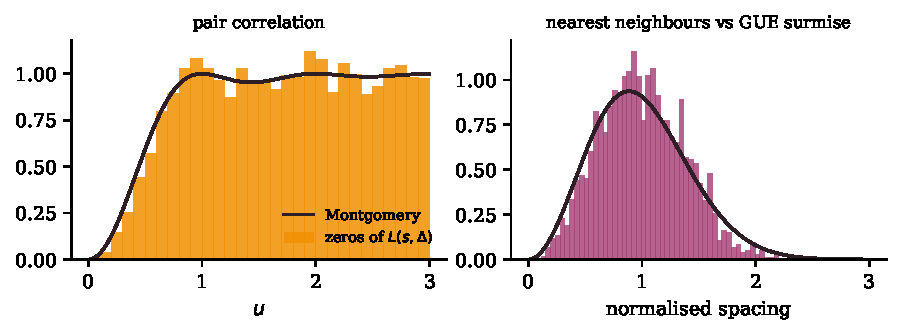
\includegraphics[width=\textwidth]{figs/delta_pair_correlation.pdf}
\caption{Zeros of $L(s,\Delta)$ with ordinates in $[500,2000]$ ($2495$ zeros, located as sign changes of $Z_\Delta$ on a grid of step $0.04$). Left: empirical pair correlation of the unfolded ordinates in bins of width $0.1$, against Montgomery's function $1-(\sin\pi u/\pi u)^2$. Right: histogram of the $2494$ normalised nearest neighbour spacings against the Wigner surmise $\frac{32}{\pi^2}s^2e^{-4s^2/\pi}$.}\label{fig:09bpair}
\end{figure}

\section{The field through the Thorin lens}\label{sec:09bthorin}

The chapters that follow reformulate $L(s,\Delta)$ in terms of a probability law, the P\'olya variable $W$ of Chapter~\ref{ch:10} with density $\Phi_\Delta(u)\propto\Delta(ie^u)e^{6u}$, its Thorin measure (Chapter~\ref{ch:10b}), and the extreme value variable $M^*$ of Chapter~\ref{ch:11}. Here we record what the results of this chapter say in that language. Everything in this section is an exact consequence of the cited theorems, and none of it is evidence for or against the Riemann hypothesis.

\begin{proposition}[Selberg's theorem as a statement about a characteristic function; this book]\label{prop:09bpolya}
Let $\varphi_W(t)=\E e^{itW}$. For real $t$,
\[
\log|L(6+it,\Delta)|=\log|\varphi_W(t)|-\log|\Gamma(6+it)|+\log\bigl(\Gamma(6)L(6,\Delta)\bigr),
\]
and, as $|t|\to\infty$,
\[
\log|L(6+it,\Delta)|=\log|\varphi_W(t)|+\frac\pi2|t|-\frac{11}2\log|t|+C_\Delta+O\Bigl(\frac1{|t|}\Bigr),
\]
with $C_\Delta=\log(120\,L(6,\Delta))-\frac12\log2\pi=3.6355$.
Consequently, under the hypothesis of Theorem~\ref{thm:09bselbergdelta}, for $t$ uniform on $[T,2T]$,
\[
\frac{\log|\varphi_W(t)|+\frac\pi2t-\frac{11}2\log t+C_\Delta}{\sqrt{\frac12\log\log T}}\Longrightarrow N(0,1).
\]
\end{proposition}

\begin{proof}
By Theorem~\ref{thm:ch10kernel}, $\varphi_W(t)=\Lambda(6+it,\Delta)/\Lambda(6,\Delta)$, and $|\Lambda(6+it,\Delta)|=(2\pi)^{-6}|\Gamma(6+it)||L(6+it,\Delta)|$, $\Lambda(6,\Delta)=(2\pi)^{-6}\Gamma(6)L(6,\Delta)$. This gives the identity. Stirling's formula $\log|\Gamma(\sigma+it)|=(\sigma-\frac12)\log|t|-\frac\pi2|t|+\frac12\log2\pi+O(1/|t|)$ at $\sigma=6$ gives the expansion, with $L(6,\Delta)=0.792123$. The last statement is Theorem~\ref{thm:09bselbergdelta} rewritten.
\end{proof}

The density $\Phi_\Delta$ extends analytically to the strip $|\operatorname{Im}u|<\frac\pi2$, since $ie^{u}$ stays in the upper half plane there, and it is this strip that forces $|\varphi_W(t)|$ to decay like $e^{-\pi|t|/2}$ up to powers of $t$. Under the Riemann hypothesis for $\Delta$, Proposition~\ref{prop:09bpolya} says that on top of this deterministic decay the characteristic function of an explicit, smooth, symmetric probability law carries lognormal fluctuations of variance $\frac12\log\log t$. By Theorem~\ref{thm:09brs} its real zeros, which are the zeros of $L(s,\Delta)$ on the critical line, have GUE correlations for test functions in the restricted range, and the heuristics of Section~\ref{sec:09blogcorr} predict that the maxima of $\log|L(6+it,\Delta)|$ over unit windows follow the Fyodorov Hiary Keating asymptotics. The same holds for the P\'olya kernel of the Riemann $\Xi$ function in Chapter~\ref{ch:10}, with the lognormal fluctuations unconditional by Theorem~\ref{thm:09bselberg} and, under the Riemann hypothesis for $\zeta$, Montgomery's theorem in place of Theorem~\ref{thm:09brs}.

Under the Riemann hypothesis for $\Delta$ the same function is a logarithmic potential. By Chapter~\ref{ch:10b} the function $s\mapsto\Lambda(6)/\Lambda(6+\sqrt s)$ is then the Laplace transform of the generalized gamma convolution $Y=\sum_kE_k/\gamma_k^2$, with $E_k$ independent standard exponentials and Thorin measure $\tau_\Delta=\sum_k\delta_{\gamma_k^2}$.

\begin{proposition}[The field as the potential of the Thorin measure; this book]\label{prop:09bpotential}
Assume the Riemann hypothesis for $L(s,\Delta)$, with zeros $6\pm i\gamma_k$, $\gamma_k>0$. For real $t\ne\pm\gamma_k$,
\[
\log|\varphi_W(t)|=\sum_k\log\Bigl|1-\frac{t^2}{\gamma_k^2}\Bigr|=\int_{(0,\infty)}\log\Bigl|1-\frac{t^2}{x}\Bigr|\,\tau_\Delta(dx)=-\log\bigl|\mathcal{L}_Y(t^2)\bigr|,
\]
where $\mathcal{L}_Y(u)=\prod_k(1-u/\gamma_k^2)^{-1}$ is the meromorphic continuation of the moment generating function $\E e^{uY}$, $u<\gamma_1^2$, to $\C$. Moreover, on each interval between consecutive zeros, $t\mapsto\log|\varphi_W(t)|$ is strictly concave.
\end{proposition}

\begin{proof}
Theorem~\ref{thm:ch10hadamard} gives $\Lambda(6+z)/\Lambda(6)=\prod_k(1+z^2/\gamma_k^2)$ for all $z$, with $\sum_k\gamma_k^{-2}<\infty$; put $z=it$ and take logarithms of absolute values, which is legitimate because the product converges absolutely. The integral is the same sum written against $\tau_\Delta$. For $u<\gamma_1^2$, independence gives $\E e^{uY}=\prod_k\E e^{uE_k/\gamma_k^2}=\prod_k(1-u/\gamma_k^2)^{-1}$, and the product converges to a meromorphic function of $u$ with simple poles at the $\gamma_k^2$. Finally $\frac{d^2}{dt^2}\log|1-t^2/\gamma^2|=-2(\gamma^2+t^2)/(\gamma^2-t^2)^2<0$, and a convergent sum of strictly concave functions is strictly concave.
\end{proof}

So, under the Riemann hypothesis, the field of this chapter is, after the archimedean drift, the logarithmic potential of the Thorin measure, evaluated at the point $t^2$ of the half line that carries the measure. The log correlated picture predicts that this potential, for atoms with sine kernel statistics, fluctuates like a log correlated Gaussian field; for random unitary matrices Hughes, Keating and O'Connell \cite{hko2001} proved that the logarithm of the characteristic polynomial along the circle converges, as a random generalised function, to such a field. The hybrid product also has a reading here, which we offer only as a heuristic: $Z_X$ involves the zeros within about $1/\log X$ of $t$, that is, the Thorin atoms within about $2t/\log X$ of $t^2$, while the potential of the far atoms is smooth in $t$ and is carried by the primes $p\le X$ through the explicit formula used in Chapter~\ref{ch:10d}. The prime and zero parts of $V_\Delta$ are then the variances of the far and near potentials.

The extreme value representation of Chapter~\ref{ch:11} is a third view of the same object. There $\Delta(iy)=e^{-2\pi y}F(y)$ with $F$ the distribution function of $M^*$, the maximum of the independent variables $E_{j,n}/(2\pi n)$, and $L(s,\Delta)=\E[Q(s,2\pi M^*)]$ (Theorem~\ref{thm:ch11main}). Proposition~\ref{prop:ch11posterior} there identifies $\Phi_\Delta$ as a conditional law; on the critical line it reads as follows.

\begin{proposition}[The critical line through $M^*$; this book]\label{prop:09bmstar}
Let $G$ have the gamma law of shape $6$ and unit rate, independent of $M^*$. For real $t$,
\[
\frac{\Gamma(6+it)}{\Gamma(6)}\,L(6+it,\Delta)=\E\bigl[G^{it}\,;\,G\ge2\pi M^*\bigr].
\]
The finite measure $\nu(B)=\Prob(\log G\in B,\ G\ge2\pi M^*)$ has total mass $L(6,\Delta)$ and equals $L(6,\Delta)$ times the law of $W+\log2\pi$.
\end{proposition}

\begin{proof}
Proposition~\ref{prop:ch11posterior}, with $G_6=G$, says that conditional on $\{G\ge2\pi M^*\}$, an event of probability $L(6,\Delta)$ by Theorem~\ref{thm:ch11main}, the variable $\log(G/2\pi)$ has density $\Phi_\Delta$, which gives the second statement. At $z=it$ the proposition yields $\E[(G/2\pi)^{it};G\ge2\pi M^*]=L(6,\Delta)\Lambda(6+it,\Delta)/\Lambda(6,\Delta)$, and $\Lambda(s,\Delta)=(2\pi)^{-s}\Gamma(s)L(s,\Delta)$ turns this into the first.
\end{proof}

So the P\'olya variable is the logarithm of a gamma variable conditioned to beat $2\pi M^*$, recentred. Two kinds of extremes should not be confused here. The variable $M^*$ is a maximum of independent exponentials on the Mellin side, and it determines $L(s,\Delta)$ for every $s$; the maxima of $\log|L(6+it,\Delta)|$ over unit windows, the analogue for $\Delta$ of Conjecture~\ref{conj:09bfhk}, are maxima of a log correlated field on the spectral side. Proposition~\ref{prop:09bmstar} writes $L(6+it,\Delta)$ as the Fourier transform of a measure built from $G$ and $M^*$, but we see no direct route from the law of $M^*$ to those maxima beyond the decay rate of Proposition~\ref{prop:09bpolya}.

\section{Notes}

Arguin, Belius and Harper~\cite{abh2017} first proved the two leading terms of Conjecture~\ref{conj:09bfhk} for a randomised model of $\zeta$, and the proofs for $\zeta$ itself collected in Theorem~\ref{thm:09bfhkproved} adapt the branching random walk methods behind Theorem~\ref{thm:09bbrw}.

Our own contributions are modest and labelled: Proposition~\ref{prop:09blefttail} (an elementary fact we use to explain the left tail), Proposition~\ref{prop:09bcov} (the covariance of the random model, a standard computation written out), Proposition~\ref{prop:09bballot} (the ballot computation in a model where it is exact), Conjecture~\ref{conj:09bvar} (the CFKRS and hybrid heuristics written out for $\Delta$, with the constant $A_\Delta$ computed), and the three propositions of Section~\ref{sec:09bthorin}. Proposition~\ref{prop:09bks} is Keating and Snaith's, in our presentation. All data in this chapter come from our PARI/GP and Python computations: the $50{,}000$ values of $\log|L(6+it,\Delta)|$, the $2000$ window maxima, the $2495$ zeros, the random field and the Steinhaus simulations, and the constants $A_\zeta$, $A_\Delta$, $B_\Delta$.

\section{Exercises}

\begin{enumerate}
\item\label{ex:09bcumulants} Using Proposition~\ref{prop:09bks}, compute $\kappa_5(\infty)$ and $\kappa_6(\infty)$ for $\log|\Lambda_N|$, and show that $(-1)^j\kappa_j(\infty)>0$ for all $j\ge3$. Deduce that, in standard units, the skewness of $\log|\Lambda_N|$ is asymptotic to $-\frac{\pi^2}4\bigl(\frac12\log N\bigr)^{-3/2}$. Compare with the data of Section~\ref{sec:09btail}.
\item\label{ex:09bmertens} Using $L(s,\Delta\times\Delta)=\zeta(s)L(s,\Sym^2\Delta)$ and the prime number theorem for $\Sym^2\Delta$, prove that
\[
A_\Delta=\log L(1,\Sym^2\Delta)-\sum_p\sum_{m\ge2}\Bigl(\frac1m-\frac1{m^2}\Bigr)\frac{(2\cos m\theta_p)^2}{p^m},
\]
and show that the analogous identity for $\zeta$ reads $A_\zeta=-\sum_p\sum_{m\ge2}(\frac1m-\frac1{m^2})p^{-m}$. Check numerically that $A_\zeta=-0.1762$ using the primes below $10^4$.
\item\label{ex:09bbridge} Prove that a Brownian bridge of variance $\sigma^2$ per unit time from $0$ to $e$ on $[0,n]$ stays below $h>\max(0,e)$ with probability $1-\exp(-2h(h-e)/(\sigma^2n))$. Using Proposition~\ref{prop:09bballot}, find $m_n$ for the $b$ ary tree with $\sigma^2=\frac12\log b$ and check that $cn$ and $\theta$ do not depend on $b$ when $n$ is measured in units of $\log b$.
\item\label{ex:09bfour} (Probabilistic.) For the Steinhaus model show that $\E|S(x)|^4$ equals the number of quadruples $(n_1,n_2,n_3,n_4)$ in $[1,x]^4$ with $n_1n_2=n_3n_4$, and that this is $\asymp x^2\log x$. Explain why this shows that $S(x)/\sqrt x$ is not asymptotically Gaussian, and why it is consistent with Theorem~\ref{thm:09bharper} by H\"older's inequality.
\item\label{ex:09bharper} Prove Lemma~\ref{lem:09bplancherel} in detail, and use it with $f(n)=1$ to show that for $\sigma>1$
\[
\int_1^\infty\frac{\lfloor u\rfloor^2}{u^{1+2\sigma}}\,du=\frac1{2\pi}\int_{-\infty}^\infty\frac{|\zeta(\sigma+it)|^2}{|\sigma+it|^2}\,dt .
\] Evaluate both sides asymptotically as $\sigma\to1^+$.
\item\label{ex:09bconcave} Assume the Riemann hypothesis for $\Delta$. Using Propositions~\ref{prop:09bpolya} and \ref{prop:09bpotential}, show that between two consecutive zeros $\gamma_k<\gamma_{k+1}$ the function $\log|L(6+it,\Delta)|$ has exactly one critical point once $\gamma_k$ is large enough. (Hint: compare the second derivative of the archimedean term with that of the potential, and use that the gaps $\gamma_{k+1}-\gamma_k$ are bounded, by the counting formula of Section~\ref{sec:09bpair}.)
\end{enumerate}

\section{Open computational problems}

\begin{compproblem}[Selberg's theorem and the hybrid constant at height $10^8$]\label{cp:09bselberg}
Objective: test Conjecture~\ref{conj:09bvar} and the cumulant predictions of Proposition~\ref{prop:09bks} for $L(s,\Delta)$ at heights where $\frac12\log\log T$ has moved appreciably. Objects and scale: $\log|L(6+it,\Delta)|$ on grids of spacing $0.01$ in windows of length $10^4$ centred at $T=10^4,10^5,10^6,10^7,10^8$ (about $10^6$ values per window), and $A_\Delta$ to five digits, from $\tau(p)$ for all $p\le10^9$ or, more cheaply, from the identity of Exercise~\ref{ex:09bmertens} with $L(1,\Sym^2\Delta)=\frac{\pi}{2}\frac{(4\pi)^{12}}{11!}\langle\Delta,\Delta\rangle$, where $\langle\Delta,\Delta\rangle=\int_{\SL_2(\Z)\backslash\mathbb H}|\Delta(\tau)|^2y^{12}\,dx\,dy/y^2$ is computed by PARI/GP \texttt{mfpetersson}. Route: an Odlyzko Sch\"onhage type multi evaluation \cite{odlyzkoschonhage1988} of the approximate functional equation for $\Delta$, or interval arithmetic in the style of Platt for certified values, checked against PARI/GP \texttt{lfun}. Deliverable: a table of sample variance, $\kappa_3$, $\kappa_4$ and their standard errors (by block bootstrap over zero spacings) against $V_\Delta(T)$ and $\kappa_j(\infty)$; and a fit of the residual $\operatorname{Var}-V_\Delta(T)$ against $1/\log T$. Why it matters: it would show whether the agreement found at $T\approx1500$ persists, and measure the lower order terms that the hybrid heuristic leaves out.
\end{compproblem}

\begin{compproblem}[The law of the maximum]\label{cp:09bmax}
Objective: estimate the distribution of $M_T-m_T$ (Theorem~\ref{thm:09bfhkproved}) for $\zeta$ and for $L(s,\Delta)$ and compare it with a randomly shifted Gumbel law. Objects and scale: $10^5$ unit windows at each of the heights $10^{10}$, $10^{16}$, $10^{22}$ for $\zeta$ and $10^5$ windows at heights up to $10^8$ for $\Delta$; in parallel, $10^6$ realisations of the Steinhaus and Sato Tate random Euler products and of a matched branching random walk, recording its derivative martingale. Route: for $\zeta$ and $\Delta$, Odlyzko Sch\"onhage multi evaluation \cite{odlyzkoschonhage1988} (for $\zeta$, also Hiary's fast algorithms) on fine grids with local refinement of maxima; for the models, GPU evaluation of truncated Euler products, and a fit of $\Prob(M\le y)$ to $\E\exp(-C^*D_\infty e^{-2y})$. Deliverable: empirical distribution functions of $M_T-m_T$, estimates of the additive constants for $\zeta$, $\Delta$ and the models, tail plots of $\log\Prob(M>y)+2y-\log y$, and a test of the shape $ye^{-2y}$. Why it matters: the limit law is the open part of Conjecture~\ref{conj:09bfhk}.
\end{compproblem}

\begin{compproblem}[Pair correlation and spacings for $\Delta$ to height $10^7$]\label{cp:09bpair}
Objective: measure the finite height corrections to the GUE statistics of the zeros of $L(s,\Delta)$. Objects and scale: all zeros with $0<\gamma\le10^5$, about $2.8\times10^5$, certified by Turing's method, and blocks of $10^5$ consecutive zeros near $\gamma=10^6$ and $10^7$. Route: PARI/GP \texttt{lfunzeros} or Rubinstein's \texttt{lcalc}, with a dense search near small gaps to recover close pairs; the Bogomolny Keating formula \cite{bogomolnykeating1996} adapted to $\Delta$, and spacing laws of small unitary matrices from Fredholm determinants. Deliverable: pair correlation residuals against $1-(\sin\pi u/\pi u)^2$ with error bands, the spacing variance as a function of height against $0.180$, and the effective matrix size for $\Delta$ that best fits the spacing law at each height, compared with the analogue of the prediction of \cite{bblm2006}. Why it matters: it would show whether finite height effects account for the narrow spacing law (variance $0.138$) observed near $t\approx10^3$, and test the arithmetic corrections in degree two.
\end{compproblem}

\begin{compproblem}[Harper's constant and critical chaos]\label{cp:09bharper}
Objective: estimate the limit of $c(x)=\E|S(x)|(\log\log x)^{1/4}/\sqrt x$ for the Steinhaus model, which exists by the theorem of Gorodetsky and Wong (Section~\ref{sec:09bharper}), and the speed of convergence; decide numerically whether $c(x)$ converges for the Rademacher model; and relate the limits to critical chaos. Objects and scale: $10^4$ realisations of each model with $x$ up to $10^{10}$, and for each realisation the total mass $\int_{-1/2}^{1/2}|F_x(\frac12+\frac1{\log x}+it)|^2dt$ of the truncated Euler product over $p\le x$. Route: segmented sieves on GPUs generating $f(n)$ from random values at primes; variance reduction by conditioning on the small primes. Deliverable: plots of $c(x)$ with confidence bands; the joint law of $S(x)/\sqrt x$ and the chaos mass, with a test of the conditional Gaussian picture of Section~\ref{sec:09bharper}; and the same for the character sums of \cite{harper2023} with $r$ prime near $10^{12}$. Why it matters: Harper's theorem gives the order of magnitude but not a constant, and we know of no closed form for the limit of $c(x)$; a numerical value of the limit, its rate of approach, and its relation to the critical measure would indicate what the next theorem should be.
\end{compproblem}

\chapter{P\'olya Kernels, Generalized Gamma Convolutions and Thorin Measures}\label{ch:10}

In 1926 P\'olya studied Riemann's $\Xi$ function as the Fourier transform of an explicit positive even kernel and asked which properties of a kernel force its transform to have only real zeros. For Riemann's kernel the question is the Riemann hypothesis, still open; it led to de Bruijn's heat flow and the de Bruijn Newman constant. Two later strands from probability, Thorin's generalized gamma convolutions and the Brownian identities surveyed by Biane, Pitman and Yor, supply the language of this chapter. We transport P\'olya's framework from $\zeta$ to an automorphic $L$ function of $\GL_2$. For the discriminant form $\Delta$ the kernel is $\Delta$ itself on the imaginary axis, read in logarithmic coordinates; the corresponding random variable has a characteristic function that vanishes at $t$ exactly when $L(6+it,\Delta)=0$; and the Riemann hypothesis for $\Delta$ becomes the statement that a certain reciprocal is the Laplace transform of a generalized gamma convolution with an explicit Thorin measure. We prove these equivalences in full. They reformulate the Riemann hypothesis for $\Delta$ without proving it, and we say exactly what is missing.

\section{The P\'olya kernel of the Riemann zeta function}

Let $\xi(s) = \frac12 s(s-1)\pi^{-s/2}\Gamma(s/2)\zeta(s)$ and $\Xi(t) = \xi(\frac12+it)$. Riemann \cite{riemann1859} observed that $\Xi$ is entire, even and real on $\R$, and the Riemann hypothesis\index{Riemann hypothesis} is the statement that all zeros of $\Xi$ are real. From the theta transformation formula one obtains
\begin{gather}
\Xi(t) = \int_{-\infty}^\infty \Phi(u)\,e^{itu}\,du,\label{eq:ch10polya}\\
\Phi(u) = 2\sum_{n\ge1}\bigl(2\pi^2n^4e^{9u/2} - 3\pi n^2e^{5u/2}\bigr)\exp\bigl(-\pi n^2e^{2u}\bigr).\notag
\end{gather}
The kernel $\Phi$ is even, strictly positive, and decays like $\exp(-\pi e^{2|u|}+\frac92|u|)$. After normalisation by $\Xi(0)$ it is the density of a symmetric random variable whose characteristic function is $\Xi(t)/\Xi(0)$.\index{P\'olya kernel}

P\'olya \cite{polya1926} proved that an explicit approximation of $\Phi$ built from its leading term has a transform with only real zeros, and in a sequel \cite{polya1927} he identified multipliers of a kernel, among them $e^{\lambda u^2}$ with $\lambda>0$, that preserve the reality of the zeros of its transform. De Bruijn \cite{debruijn1950} made the second idea quantitative. Put
\[
H_\lambda(z) = \int_{-\infty}^\infty e^{\lambda u^2}\Phi(u)\,e^{izu}\,du ,
\]
so that $H_0=\Xi$. If all zeros of $H_0$ lie in the strip $|\operatorname{Im}z|\le b_0$, then for $\lambda>0$ all zeros of $H_\lambda$ lie in $|\operatorname{Im}z|\le\sqrt{\max(b_0^2-2\lambda,0)}$. For $\Xi$ one may take $b_0=\frac12$, so $H_\lambda$ has only real zeros for $\lambda\ge\frac18$.\index{heat flow} Newman \cite{newman1976} showed that there is a real constant $\lambda_0$ such that $H_\lambda$ has only real zeros exactly when $\lambda\ge\lambda_0$, and conjectured $\lambda_0\ge0$; the Riemann hypothesis is the statement $\lambda_0\le0$. The literature normalises the heat flow by $H_0(z)=\frac18\Xi(z/2)$, in which the threshold is the de Bruijn Newman constant\index{de Bruijn Newman constant} $\Lambda=4\lambda_0$ and de Bruijn's bound reads $\Lambda\le\frac12$. Rodgers and Tao \cite{rodgerstao2020} proved Newman's conjecture $\Lambda\ge0$, and the Polymath project \cite{polymath2019} proved $\Lambda\le0.22$.

\subsection{The Laguerre P\'olya class and P\'olya frequency functions}

An entire function belongs to the \emph{Laguerre P\'olya class}\index{Laguerre P\'olya class} if it is a locally uniform limit of real polynomials with only real zeros; by the theorem of Laguerre and P\'olya these are the real entire functions of genus at most one with only real zeros, times a factor $e^{-\gamma z^2}$ with $\gamma\ge0$ \cite{levin1964}. The Riemann hypothesis is the statement that $\Xi$ is in the Laguerre P\'olya class. A function $f$ on $\R$ is a \emph{P\'olya frequency function}\index{P\'olya frequency function} of infinite order if every determinant $\det[f(x_i-y_j)]$ with $x_1<\dots<x_n$ and $y_1<\dots<y_n$ is nonnegative.

\begin{theorem}[Schoenberg]\label{thm:ch10schoenberg}
An integrable function $f$ on $\R$, not almost everywhere zero, is a P\'olya frequency function of infinite order if and only if its bilateral Laplace transform is $\int e^{-sx}f(x)\,dx = 1/\Psi(s)$ in a vertical strip containing the imaginary axis, with
\[
\Psi(s) = Ce^{-\gamma s^2+\delta s}\prod_k(1+\delta_ks)e^{-\delta_ks},
\]
where $C>0$, $\gamma\ge0$, $\delta,\delta_k\in\R$ and $0<\gamma+\sum_k\delta_k^2<\infty$.
\end{theorem}

The functions $\Psi$ in Schoenberg's theorem \cite{schoenberg1951,karlin1968} are exactly the members of the Laguerre P\'olya class that are positive at the origin and not of the form $Ce^{\delta s}$. Thus a real entire function $\Psi$ with $\Psi(0)>0$, equal to $e^{-\gamma s^2}$ with $\gamma\ge0$ times a function of genus at most one and not of the form $Ce^{\delta s}$, has only real zeros exactly when $1/\Psi$ is, near the imaginary axis, the bilateral Laplace transform of a P\'olya frequency function.

\section{Gamma convolutions and Thorin measures}

\begin{definition}\label{def:ch10ggc}
A probability law on $[0,\infty)$ is a \emph{generalized gamma convolution}\index{generalized gamma convolution} (GGC) if it is a weak limit of finite convolutions of gamma laws. Equivalently \cite{thorin1977,bondesson1992}, its Laplace transform is
\[
\varphi(s) = \exp\Bigl(-as - \int_{(0,\infty)}\log\Bigl(1+\frac{s}{t}\Bigr)\,\tau(dt)\Bigr),\qquad s\ge0,
\]
with $a\ge0$ and a positive measure $\tau$ on $(0,\infty)$, finite on compact sets, the \emph{Thorin measure}\index{Thorin measure}, satisfying $\int_{(0,1]}|\log t|\,\tau(dt)<\infty$ and $\int_{(1,\infty)}t^{-1}\,\tau(dt)<\infty$. These conditions say exactly that the integral in the exponent is finite for $s>0$.
\end{definition}

By Frullani's integral $\log(1+s/t) = \int_0^\infty(1-e^{-sx})e^{-tx}x^{-1}\,dx$, so a GGC is infinitely divisible with drift $a$ and L\'evy measure $k(x)x^{-1}dx$, where
\[
k(x) = \int e^{-tx}\,\tau(dt)
\]
is completely monotone. Conversely an infinitely divisible law on $[0,\infty)$ whose L\'evy measure has density $k(x)/x$ with $k$ completely monotone is a GGC, and $\tau$ is the Bernstein measure of $k$. A gamma law with shape $\alpha$ and rate $t$ has Thorin measure $\alpha\delta_t$. GGCs are self decomposable, hence unimodal, and the class is closed under convolution and weak limits \cite{bondesson1992}.

\begin{lemma}\label{lem:ch10nonvanish}
The Laplace transform of a GGC extends to a holomorphic function on $\C\setminus(-\infty,0]$ with no zeros there.
\end{lemma}

\begin{proof}
For $s$ in a compact $K\subset\C\setminus(-\infty,0]$ and $t>0$, the number $1+s/t$ avoids $(-\infty,0]$, so the principal logarithm $\log(1+s/t) = \log(t+s)-\log t$ is holomorphic in $s$. It is bounded by $2|s|/t$ for $t\ge2\max_K|s|$, by $|\log t|+C_K$ for $t\le1$, and by a constant on the compact range between. By the conditions on $\tau$ the integral converges absolutely and uniformly on $K$, so the exponent is holomorphic on $\C\setminus(-\infty,0]$, it agrees with $\log\varphi$ for $s>0$, and its exponential has no zeros.
\end{proof}

\subsection{Brownian motion and the Riemann $\xi$ function}\label{sec:ch10bpy}

Biane, Pitman and Yor \cite{bpy2001} survey a probabilistic reading of $\xi$ through Brownian motion. Let $T$ be the first hitting time of $1$ by a three dimensional Bessel process started at $0$. Then $\E e^{-\lambda T} = \sqrt{2\lambda}/\sinh\sqrt{2\lambda}$, and the product formula for $\sinh$ gives
\[
\E e^{-\lambda(T+\hat T)} = \Bigl(\frac{\sqrt{2\lambda}}{\sinh\sqrt{2\lambda}}\Bigr)^2 = \prod_{n\ge1}\Bigl(1+\frac{2\lambda}{\pi^2n^2}\Bigr)^{-2}
\]
for an independent copy $\hat T$. Hence $T+\hat T$ is a GGC with Thorin measure $2\sum_n\delta_{\pi^2n^2/2}$: it has the law of $\sum_n 2G_n/(\pi^2n^2)$ with $G_n$ independent gamma variables of shape $2$. The variable $Y = \sqrt{\pi(T+\hat T)/2}$, which has the law of $\sqrt{2/\pi}$ times the maximum of a standard Brownian excursion, satisfies
\[
\E[Y^s] = 2\xi(s)\qquad\text{for all } s\in\C .
\]
The functional equation $\xi(s)=\xi(1-s)$ becomes a distributional identity for $Y$, and the Euler product plays no role. The identity $\xi(\frac12+z)/\xi(\frac12) = \E[Y^{1/2+z}]/\E[Y^{1/2}]$ shows that P\'olya's density $\Phi/\Xi(0)$ is the density of $\log Y$ when the law of $Y$ is size biased by $Y^{1/2}$. Theorem~\ref{thm:ch10kernel} below gives the analogue for $\Delta$: $\E[(e^W)^{s-6}] = \Lambda(s,\Delta)/\Lambda(6,\Delta)$, and the functional equation is the symmetry of $W$.

\subsection{The reciprocal Xi function}

The first author \cite{polson2017} studied the reciprocal of $\Xi$ in the variable $\sqrt s$. Since $\Xi$ is even and of order one, $t\mapsto\Xi(\sqrt t)$ is entire of order one half, and if all zeros of $\Xi$ are real, say $\pm\gamma_k$ with $\gamma_k>0$, Hadamard's theorem gives
\[
\frac{\xi(\frac12)}{\xi(\frac12+\sqrt s)} = \prod_k\Bigl(1+\frac{s}{\gamma_k^2}\Bigr)^{-1},
\]
which is the Laplace transform of the GGC $\sum_kE_k/\gamma_k^2$, with $E_k$ independent standard exponential variables and Thorin measure $\sum_k\delta_{\gamma_k^2}$; conversely the GGC property forces the zeros onto the line, by the argument of Theorem~\ref{thm:ch10ggc} below. That paper develops this Thorin representation, its L\'evy measure and a transform taking the L\'evy measure of the primal function to the Thorin measure of its reciprocal, as a route to Hilbert's eighth problem. It does not prove the Riemann hypothesis, and neither does this book; what it supplies is a dictionary in which the Riemann hypothesis is a positivity statement. We now build the same dictionary for the discriminant form, where each identity can be checked numerically.

\section{The P\'olya kernel of the discriminant form}

Let $\Delta(\tau) = q\prod_{n\ge1}(1-q^n)^{24} = \sum_n\tau(n)q^n$ with $q = e^{2\pi i\tau}$, the cusp form of weight $12$ for $\SL_2(\Z)$. We use the classical normalisation of Chapter~\ref{ch:02}: $L(s,\Delta) = \sum_n\tau(n)n^{-s}$ and $\Lambda(s,\Delta) = (2\pi)^{-s}\Gamma(s)L(s,\Delta)$, which is entire with $\Lambda(s,\Delta) = \Lambda(12-s,\Delta)$ by Hecke's Theorem~\ref{thm:02fe}, so the centre is $s=6$. All zeros of $\Lambda(s,\Delta)$ lie in $\frac{11}{2}<\operatorname{Re}s<\frac{13}{2}$ (Section~\ref{sec:02mellin}; on the line $\operatorname{Re}s=\frac{13}{2}$ this is Proposition~\ref{prop:ch09nonvanish} away from $s=\frac{13}{2}$ and Proposition~\ref{prop:ch10mellin} below at $s=\frac{13}{2}$), and the Riemann hypothesis for $\Delta$ is the conjecture that they all lie on $\operatorname{Re}s=6$.

\begin{proposition}\label{prop:ch10mellin}
For all $s\in\C$,
\[
\Lambda(s,\Delta) = \int_0^\infty\Delta(iy)\,y^{s-1}\,dy,
\]
with $\Delta(iy) = e^{-2\pi y}\prod_n(1-e^{-2\pi ny})^{24}>0$ for $y>0$ and $\Delta(i/y) = y^{12}\Delta(iy)$. In particular $\Lambda(\sigma,\Delta)>0$ for real $\sigma$.
\end{proposition}

\begin{proof}
Section~\ref{sec:02mellin} gives the identity for $\operatorname{Re}s>7$. The proof of Theorem~\ref{thm:02fe} gives $\Delta(i/y) = y^{12}\Delta(iy)$ and shows that $\Delta(iy)$ decays faster than any power of $y$ at both ends, so the integral converges absolutely for every $s$ and defines an entire function, which equals $\Lambda$ by analytic continuation. Positivity of $\Delta(iy)$ is clear from the product, and for real $\sigma$ the integrand is positive.
\end{proof}

Substitute $y = e^u$. The function $g(u) = \Delta(ie^u)e^{6u}$ satisfies $g(-u) = \Delta(ie^{-u})e^{-6u} = e^{12u}\Delta(ie^u)e^{-6u} = g(u)$, and $\int g = \Lambda(6,\Delta)$.

\begin{definition}
The \emph{P\'olya kernel of $\Delta$} is the probability density
\[
\Phi_\Delta(u) = \frac{\Delta(ie^u)\,e^{6u}}{\Lambda(6,\Delta)},\qquad u\in\R,
\]
and $W$, the \emph{P\'olya variable} of $\Delta$, is a random variable with density $\Phi_\Delta$.
\end{definition}

The numbers are $L(6,\Delta) = 0.792123$ and
\[
\Lambda(6,\Delta) = 120\,L(6,\Delta)/(2\pi)^6 = 0.0015449.
\] The kernel is even, strictly positive, and decays doubly exponentially, $\Phi_\Delta(u)\asymp\exp(-2\pi e^{|u|}+6|u|)$. Figure~\ref{fig:deltakernel} compares it with the normal density of the same variance. The two are close: the peak $\Phi_\Delta(0)=1.1557$ lies below the normal peak $1.1902$, and under the Riemann hypothesis for $\Delta$ the kernel is platykurtic (Exercise~\ref{ex:ch10kurtosis}). Its tails, too small to see at this scale, are far lighter than Gaussian ones.


\begin{figure}[t]
\centering
\begin{minipage}[t]{0.48\textwidth}\centering
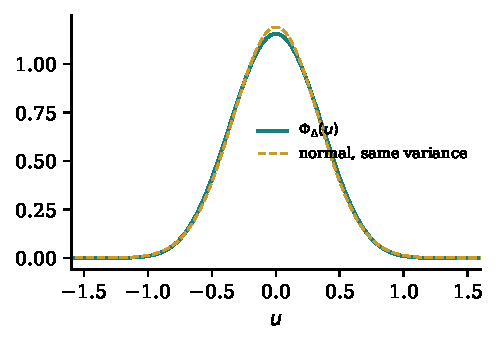
\includegraphics[width=\textwidth]{figs/deltakernel.pdf}
\caption{The kernel $\Phi_\Delta$ against the normal density with the same variance $0.112352$.}\label{fig:deltakernel}
\end{minipage}\hfill
\begin{minipage}[t]{0.48\textwidth}\centering
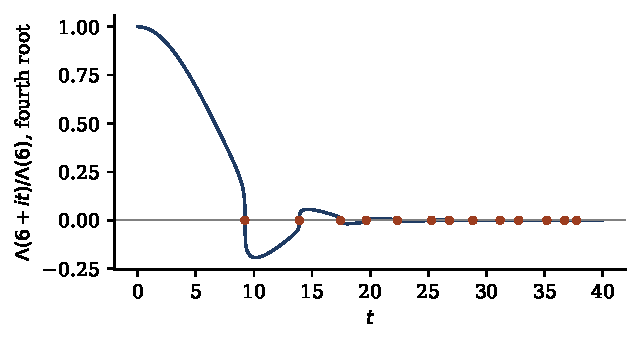
\includegraphics[width=\textwidth]{figs/deltazeros.pdf}
\caption{The characteristic function $\E e^{itW} = \Lambda(6+it,\Delta)/\Lambda(6,\Delta)$ for $0\le t\le40$, plotted as a signed fourth root to make the decaying oscillations visible, with its zeros $\gamma_k$ marked.}\label{fig:deltazeros}
\end{minipage}
\end{figure}

\begin{theorem}[this book]\label{thm:ch10kernel}
The random variable $W$ is symmetric, has moments of all orders and an entire moment generating function, and for all $z\in\C$
\[
\E\bigl[e^{zW}\bigr] = \frac{\Lambda(6+z,\Delta)}{\Lambda(6,\Delta)} .
\]
In particular $\E[e^{itW}] = \Lambda(6+it,\Delta)/\Lambda(6,\Delta)$ is real and even, and the Riemann hypothesis for $\Delta$ is equivalent to the statement that the characteristic function of $W$ has only real zeros.
\end{theorem}

\begin{proof}
By Proposition~\ref{prop:ch10mellin} for $s = 6+z$ and $y = e^u$, $\Lambda(6+z) = \int g(u)e^{zu}\,du$, which converges absolutely for all $z$ by the doubly exponential decay of $g$; dividing by $\Lambda(6)$ gives the identity. Symmetry of $\Phi_\Delta$ makes the characteristic function real and even. Zeros of $\Lambda(s,\Delta)$ are the points $6+it$ with $\E e^{itW}=0$, and they lie on $\operatorname{Re}s=6$ exactly when the corresponding $t$ is real.
\end{proof}

Our computations for this book located $404$ zeros of $\Lambda(6+it,\Delta)$ on the critical line with $0<t\le400$, the first six being
\[
9.22238,\quad 13.90755,\quad 17.44278,\quad 19.65651,\quad 22.33610,\quad 25.27464 .
\]
For the number $N(T)$ of zeros $6+i\gamma$ with $0<\gamma\le T$, the Riemann von Mangoldt formula for $\Delta$ reads $N(T) = \frac{T}{\pi}\log\frac{T}{2\pi e}+\frac{11}{4}+O(\log T)$, where the error term is $\frac1\pi\arg L(6+iT,\Delta)$ up to $O(1/T)$; the main terms give $404.3$ at $T=400$. The characteristic function computed by quadrature against $\Phi_\Delta$ agrees with $\Lambda(6+it)/\Lambda(6)$ to at least twelve significant digits at $t = 2,5,12$, and at $t=\gamma_1$ its computed value is $1.2\times10^{-17}$. Figure~\ref{fig:deltazeros} shows it.


\subsection{The Hadamard product and the variance identity}

The zeros of $\Lambda(6+z,\Delta)$ are symmetric under $z\mapsto-z$ and $z\mapsto\bar z$, since $\Lambda(6+z)$ is even and real for real $z$, and none is real, since $\Lambda(6+x)>0$. Writing a zero as $z = i\gamma$, we list one representative of each pair $\{\gamma,-\gamma\}$ with $\operatorname{Re}\gamma>0$ as $\gamma_1,\gamma_2,\dots$, with multiplicity and in order of increasing real part. The Riemann hypothesis for $\Delta$ says all $\gamma_k$ are real.

\begin{theorem}[this book]\label{thm:ch10hadamard}
Unconditionally, $\sum_k|\gamma_k|^{-2}<\infty$ and for all $z\in\C$
\[
\frac{\Lambda(6+z,\Delta)}{\Lambda(6,\Delta)} = \prod_k\Bigl(1+\frac{z^2}{\gamma_k^2}\Bigr).
\]
Consequently $\E W = 0$ and
\[
\operatorname{Var}W = 2\sum_k\frac{1}{\gamma_k^2},
\]
where the right side is real because nonreal $\gamma_k$ occur in conjugate pairs.
\end{theorem}

\begin{proof}
Since $\Delta(iy)>0$, Proposition~\ref{prop:ch10mellin} gives $|\Lambda(s)|\le\Lambda(\operatorname{Re}s)$ for every $s$. For real $\sigma\ge7$ we have $L(\sigma,\Delta)\le\sum_n|\tau(n)|n^{-7}<\infty$ and $\Gamma(\sigma)\le\sigma^\sigma$, and $\Lambda(\sigma) = \Lambda(12-\sigma)$; hence $|\Lambda(6+z)|\le\Lambda(6+|\operatorname{Re}z|)\le C\exp\bigl((|z|+7)\log(|z|+7)\bigr)$, and $\Lambda(6+z)$ is entire of order at most one. Define $G(w) = \Lambda(6+\sqrt w)/\Lambda(6)$. It is well defined because $\Lambda(6+z)$ is even, it is entire because an even power series in $z$ is a power series in $w = z^2$, and $|G(w)|\le C'\exp\bigl((|w|^{1/2}+7)\log(|w|^{1/2}+7)\bigr)$, so $G$ has order at most one half (exactly one half, by Stirling's formula on the real axis). Its zeros are the points $w_k = -\gamma_k^2$, with multiplicity, and $G(0) = 1$. An entire function of order less than one has genus zero, so Hadamard's theorem gives $G(w) = \prod_k(1-w/w_k)$ with $\sum_k|w_k|^{-1}<\infty$, with no exponential factor and with constant $G(0)=1$. This is the convergence statement and, with $w = z^2$, the product formula. Finally $G(w) = \E[e^{\sqrt wW}] = \sum_n\E[W^{2n}]w^n/(2n)!$ since odd moments vanish, so $G'(0) = \frac12\E W^2$, while the absolutely convergent product gives $G'(0) = \sum_k\gamma_k^{-2}$.
\end{proof}

The variance identity equates a moment of the kernel with a sum over zeros, a trace formula in miniature. Quadrature against $\Phi_\Delta$ gives $\operatorname{Var}W = 0.112352$. The $404$ computed zeros give $2\sum_{\gamma_k\le400}\gamma_k^{-2} = 0.104146$. The density of zeros at height $t$ is $\frac1\pi\log\frac{t}{2\pi}$, so the tail $\sum_{\gamma_k>T}\gamma_k^{-2}$ is approximately $\int_T^\infty\frac{\log(t/2\pi)}{\pi t^2}\,dt = \frac{\log(T/2\pi)+1}{\pi T}$, which at $T = 400$ is $0.004101$; doubling and adding gives $0.112348$, a relative difference of $3\times10^{-5}$.

\section{The Riemann hypothesis for $\Delta$ as a GGC property}

\begin{theorem}[this book]\label{thm:ch10ggc}
The following are equivalent.
\begin{enumerate}
\item[(i)] All zeros of $\Lambda(s,\Delta)$ lie on the line $\operatorname{Re}s = 6$.
\item[(ii)] The function $s\mapsto\Lambda(6,\Delta)/\Lambda(6+\sqrt s,\Delta)$, $s>0$, is the Laplace transform of a generalized gamma convolution.
\end{enumerate}
When they hold, the GGC has drift $0$ and Thorin measure $\sum_k\delta_{\gamma_k^2}$, it is the law of
\[
X = \sum_k\frac{E_k}{\gamma_k^2}
\]
with $E_k$ independent standard exponential variables, and its L\'evy measure has density
\[
\frac{k(x)}{x},\qquad k(x) = \sum_ke^{-\gamma_k^2x},
\]
which is completely monotone.
\end{theorem}

\begin{proof}
Let $G$ be as in the proof of Theorem~\ref{thm:ch10hadamard}, so the function in (ii) is $1/G(s)$ for $s>0$.

(ii) implies (i). Let $\varphi$ be the Laplace transform of the GGC. By Lemma~\ref{lem:ch10nonvanish}, $\varphi$ is holomorphic and zero free on $\C\setminus(-\infty,0]$. The function $\varphi G$ is holomorphic on this connected domain and equals $1$ on $(0,\infty)$, hence everywhere by the identity theorem, so $G$ has no zeros off $(-\infty,0]$. The zeros of $G$ are the points $-\gamma_k^2$, and $G(0) = 1$, so every $\gamma_k^2$ is a positive real number. As $\operatorname{Re}\gamma_k>0$, every $\gamma_k$ is real, and the zeros $6\pm i\gamma_k$ lie on $\operatorname{Re}s=6$.

(i) implies (ii). If all $\gamma_k$ are real, hence positive, Theorem~\ref{thm:ch10hadamard} gives $1/G(s) = \prod_k(1+s/\gamma_k^2)^{-1}$ for $s>0$. Each factor is the Laplace transform of $E_k/\gamma_k^2$. Since $\sum_k\E[E_k/\gamma_k^2] = \sum_k\gamma_k^{-2}<\infty$, the series $X$ converges almost surely and in $L^1$, and by independence and dominated convergence its Laplace transform is the infinite product. Writing the product as $\exp(-\sum_k\log(1+s/\gamma_k^2))$ exhibits it in the form of Definition~\ref{def:ch10ggc} with $a = 0$ and $\tau = \sum_k\delta_{\gamma_k^2}$. The conditions on $\tau$ hold: $\sum_k\gamma_k^{-2}<\infty$ leaves only finitely many atoms $\gamma_k^2$ below any bound, so $\tau$ is finite on compact sets and $\int_{(0,1]}|\log t|\,\tau(dt)$ is a finite sum, while $\int t^{-1}\,\tau(dt) = \sum_k\gamma_k^{-2}<\infty$. Frullani's integral gives the L\'evy density. The series $k(x)$ converges for $x>0$ because $e^{-\gamma_k^2x}\le(\gamma_k^2x)^{-1}$, and $k$ is completely monotone as the Laplace transform of the positive measure $\tau$.
\end{proof}

The first Thorin atoms are
\[
\gamma_k^2 = 85.05,\quad 193.42,\quad 304.25,\quad 386.38,\quad 498.90,\quad 638.81 .
\] Figure~\ref{fig:ggc} compares the product over the computed zeros, with the tail correction of the previous section in the exponent, to the exact value $\Lambda(6)/\Lambda(6+\sqrt s)$. The pairs (exact, corrected product over the $404$ zeros) are $(0.945467, 0.945468)$ at $s=1$, $(0.575602, 0.575612)$ at $s=10$, $(0.0069732, 0.0069741)$ at $s=100$ and $(5.6354, 5.6359)\times10^{-8}$ at $s=400$: a relative error below $2\times10^{-4}$ over more than seven orders of magnitude. Figure~\ref{fig:levydelta} shows $k$; under the Riemann hypothesis for $\Delta$, $k(x)/x$ is the L\'evy density. As $x\to0$ the zero density $\frac1\pi\log\frac{t}{2\pi}$ gives
\[
k(x) = \frac{\log(1/x)-c_0+o(1)}{4\sqrt{\pi x}},\qquad c_0 = \log(16\pi^2)+\gamma_{\mathrm E} = 5.639,
\]
with $\gamma_{\mathrm E}$ Euler's constant. The constant matters at the scale of Figure~\ref{fig:levydelta}: at $x=10^{-4}$ the numerator is about $3.57$, against $9.21$ for $\log(1/x)$ alone. The L\'evy density therefore behaves like $x^{-3/2}\log(1/x)/(4\sqrt\pi)$ at the origin: the L\'evy measure is infinite, while its first moment near the origin, $\int_0^1k(x)\,dx$, is finite, as for every subordinator.



\begin{figure}[t]
\centering
\begin{minipage}[t]{0.48\textwidth}\centering
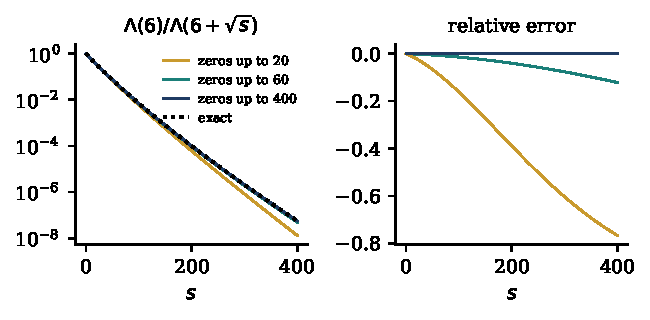
\includegraphics[width=\textwidth]{figs/ggc.pdf}
\caption{Left: the product $\prod_k(1+s/\gamma_k^2)^{-1}$ over the zeros up to height $20$, $60$ and $400$, each with its tail correction, against $\Lambda(6,\Delta)/\Lambda(6+\sqrt s,\Delta)$ (log scale). Right: the relative errors.}\label{fig:ggc}
\end{minipage}\hfill
\begin{minipage}[t]{0.48\textwidth}\centering
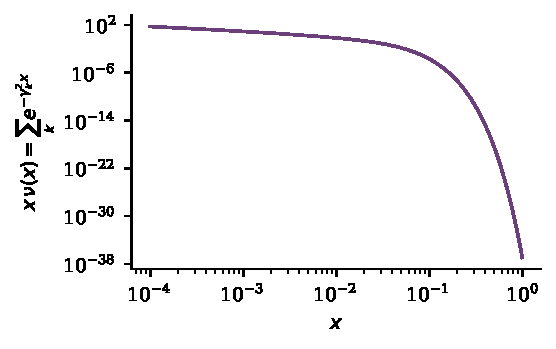
\includegraphics[width=\textwidth]{figs/levydelta.pdf}
\caption{The function $k(x) = \sum_k e^{-\gamma_k^2x}$ over the $404$ zeros up to height $400$, for $10^{-4}\le x\le1$ on log scales; under the Riemann hypothesis for $\Delta$ it is $x\nu(x)$, with $\nu$ the L\'evy density.}\label{fig:levydelta}
\end{minipage}
\end{figure}

\begin{remark}[A dual pair]\label{rem:ch10dual}
Under the Riemann hypothesis for $\Delta$ let $V = \sqrt{2X}\,N$ with $N$ standard normal independent of $X$. Then $\E e^{itV} = \E e^{-t^2X} = \Lambda(6)/\Lambda(6+t)$ for real $t$: on the real axis, the reciprocal of the moment generating function of $W$ is the characteristic function of $V$. The bilateral Laplace transform of $V$ is $1/\prod_k(1-s^2/\gamma_k^2)$ in the strip $|\operatorname{Re}s|<\gamma_1$, so by Theorem~\ref{thm:ch10schoenberg}, with $\delta_k = \pm\gamma_k^{-1}$, the density of $V$ is a P\'olya frequency function of infinite order. Conversely, if $\Lambda(6)/\Lambda(6+t)$ were the characteristic function of a P\'olya frequency density, Schoenberg's theorem would put $\prod_k(1-s^2/\gamma_k^2)$ in the Laguerre P\'olya class and all $\gamma_k$ would be real.
\end{remark}

\subsection{General self dual $L$ functions and the rank}

Apart from the variance identity, the proofs of Theorems~\ref{thm:ch10hadamard} and~\ref{thm:ch10ggc} used only that $\Lambda(6+z)$ is entire of order at most one, even, real on the real axis and nonzero at $z=0$; positivity of the kernel served only to bound the order quickly and to give the probabilistic reading of Theorem~\ref{thm:ch10kernel}. Let $\pi$ be a self dual cuspidal automorphic representation of $\GL_n(\A_\Q)$, $n\ge2$, with completed $L$ function $\Lambda(s,\pi)$ in the unitary normalisation, conductor included, so that $\Lambda(s,\pi)$ is entire of order one \cite{godementjacquet1972} and $\Lambda(s,\pi) = \varepsilon\Lambda(1-s,\pi)$ with $|\varepsilon|=1$. Self duality makes $\Lambda(s,\pi)$ real on the real axis, and then $\varepsilon=\pm1$.

\begin{theorem}[this book]\label{thm:ch10general}
Suppose $\Lambda(\frac12,\pi)\ne0$. Then the generalized Riemann hypothesis for $\pi$ holds if and only if $s\mapsto\Lambda(\frac12,\pi)/\Lambda(\frac12+\sqrt s,\pi)$ is the Laplace transform of a GGC, and then its Thorin measure is $\sum_k\delta_{\gamma_k^2}$ over the ordinates $\gamma_k>0$ of the zeros $\frac12\pm i\gamma_k$.
\end{theorem}

\begin{proof}
Since $\Lambda(\frac12)\ne0$ the functional equation at $s=\frac12$ forces $\varepsilon = 1$, so $\Lambda(\frac12+z)$ is even, and by the paragraph before the theorem the proofs of Theorems~\ref{thm:ch10hadamard} and~\ref{thm:ch10ggc} apply to $G(w) = \Lambda(\frac12+\sqrt w)/\Lambda(\frac12)$. The one new case is a real zero $\frac12+x$ of $\Lambda$, which would give a zero $x^2>0$ of $G$; the GGC property excludes it too. Theorem~\ref{thm:10babstract} gives the general argument and the other equivalent forms.
\end{proof}

When $\Lambda(\frac12+z,\pi)$ vanishes to order $r\ge1$ at $z=0$, the functional equation forces $\varepsilon=(-1)^r$, the argument applies to the even function $\Lambda(\frac12+z,\pi)/z^r$, and under the generalized Riemann hypothesis $1/\Lambda(\frac12+\sqrt s,\pi)$ is a constant times $s^{-r/2}$ times a GGC transform. The factor $s^{-r/2}$ is a degenerate Thorin atom of mass $r/2$ at the origin\index{Thorin atom at zero}, half the analytic rank for an elliptic curve; Proposition~\ref{prop:10brank} proves this, and Chapter~\ref{ch:10b} extends Theorem~\ref{thm:ch10general} to every cuspidal $\pi$, self dual or not.

\section{What is known unconditionally}

The product of Theorem~\ref{thm:ch10hadamard} splits as
\[
\frac{\Lambda(6,\Delta)}{\Lambda(6+\sqrt s,\Delta)} = \prod_{\gamma_k\in\R}\Bigl(1+\frac{s}{\gamma_k^2}\Bigr)^{-1}\times\prod_{\gamma_k\notin\R}\Bigl(1+\frac{s}{\gamma_k^2}\Bigr)^{-1}.
\]
The first factor is always a GGC transform, the law of $\sum E_k/\gamma_k^2$ over real $\gamma_k$. The second collects off line zeros in conjugate pairs. For one pair write $\gamma^2 = a+ib$ with $b\ne0$; then for $s>-a$
\begin{align*}
\Bigl(1+\frac{s}{\gamma^2}\Bigr)^{-1}\Bigl(1+\frac{s}{\bar\gamma^2}\Bigr)^{-1} &= \frac{|\gamma|^4}{(s+a)^2+b^2}\\
&= \int_0^\infty e^{-sx}\,\frac{|\gamma|^4}{b}\,e^{-ax}\sin(bx)\,dx,
\end{align*}
the Laplace transform of a function that changes sign. The Riemann hypothesis for $\Delta$ is the statement that the signed part is empty.

How much of the Thorin measure is known to be positive? Hafner \cite{hafner1983} proved, following the method of Selberg for $\zeta$ \cite{selberg1942}, that a positive proportion of the zeros of the $L$ function of a holomorphic Hecke eigenform for $\SL_2(\Z)$, counted by height, lie on the critical line. In our language, a positive proportion of the atoms $\gamma_k^2$ lie on $(0,\infty)$. But no proportion short of all of them yields the GGC property, because a single conjugate pair of nonreal $\gamma$ already destroys it, by Theorem~\ref{thm:ch10ggc}. For $\zeta$ the proportion is above two fifths \cite{conrey1989}, with the same caveat.

The heat flow transfers as well. Put $H^\Delta_\lambda(z) = \int e^{\lambda u^2}\Phi_\Delta(u)e^{izu}\,du$, so that $H^\Delta_0(z) = \Lambda(6+iz)/\Lambda(6)$. All zeros of $H^\Delta_0$ lie in $|\operatorname{Im}z|<\frac12$, so by de Bruijn's theorem $H^\Delta_\lambda$ has only real zeros for $\lambda\ge\frac18$. Dobner \cite{dobner2021}, by a method different from that of Rodgers and Tao, proved that every member of the extended Selberg class has a de Bruijn Newman constant and that it is nonnegative. The function $L(s,\Delta)$, in the unitary normalisation, belongs to that class, and Dobner's heat parameter is $4\lambda$ in our normalisation. Hence there is a constant $\lambda_\Delta$ with $0\le\lambda_\Delta\le\frac18$ such that $H^\Delta_\lambda$ has only real zeros exactly when $\lambda\ge\lambda_\Delta$, and the Riemann hypothesis for $\Delta$ is the statement $\lambda_\Delta=0$; Dobner's constant for $\Delta$ is $4\lambda_\Delta$, as $\Lambda=4\lambda_0$ for $\zeta$.\index{de Bruijn Newman constant}

\begin{remark}
Why is this a reformulation and not a proof? Every equivalence above passes through the Hadamard product, that is, through the zeros themselves. A proof of the Riemann hypothesis along these lines would need an independent construction of a GGC with Laplace transform $\Lambda(6)/\Lambda(6+\sqrt s)$, for example a stochastic process whose hitting times or occupation laws have that transform, as the Bessel hitting time $T$ of Section~\ref{sec:ch10bpy} has the transform $\sqrt{2\lambda}/\sinh\sqrt{2\lambda}$, a GGC whose Thorin atoms $\pi^2n^2/2$ come from the zeros $\pm i\pi n$ of $\sinh z/z$ (Exercise~\ref{ex:ch10bessel}). The Euler product gives positivity of a different kind, the infinite divisibility of Chapter~\ref{ch:09}, which holds only to the right of the critical strip and, for $\Delta$, holds for the Rankin Selberg function $L(s,\Delta\times\Delta)$ but not for $L(s,\Delta)$ itself: the logarithmic coefficients of $L(s,\Delta)$ change sign, and for $\sigma>\frac{13}{2}$ the function $t\mapsto L(\sigma+it,\Delta)/L(\sigma,\Delta)$ is not even a characteristic function (Proposition~\ref{prop:ch09notcf}). The GGC property is a positivity statement about the reciprocal inside the strip, and no bridge between the two is known.
\end{remark}

\begin{problem}[Hilbert's eighth problem for $\GL_2$]
Construct, without reference to the zeros, a random variable whose Laplace transform is $\Lambda(6,\Delta)/\Lambda(6+\sqrt s,\Delta)$ and prove that it is a GGC; more generally do this for every self dual cuspidal $\pi$ with $\Lambda(\frac12,\pi)\ne0$. A positive solution for one $\pi$ would prove the generalized Riemann hypothesis for that $\pi$.
\end{problem}

\section{Notes}

P\'olya's kernel and real zero theorems are in \cite{polya1926,polya1927}, the heat flow in \cite{debruijn1950,newman1976,rodgerstao2020,polymath2019}, its extension to the extended Selberg class in \cite{dobner2021}, and total positivity in \cite{schoenberg1951,karlin1968}. Thorin \cite{thorin1977,thorin1977b} introduced generalized gamma convolutions to prove that the Pareto and lognormal laws are infinitely divisible, and Bondesson's monograph \cite{bondesson1992} is the standard reference. The Brownian interpretation of $\xi$ and its relatives is the subject of the survey of Biane, Pitman and Yor \cite{bpy2001}. The Thorin representation of the reciprocal $\Xi$ function is from the first author \cite{polson2017}, and his later paper \cite{polson2018vdp} proves the equivalence of real zeros and the Thorin property for real entire functions of order at most one, with applications to Dirichlet and modular $L$ functions. Theorems~\ref{thm:ch10kernel}, \ref{thm:ch10hadamard}, \ref{thm:ch10ggc} and \ref{thm:ch10general} are elementary consequences of Hecke's theory and Hadamard's factorisation, and we present them as the book's formulation of P\'olya's programme for $\GL_2$. The numerical values were computed for this book with PARI/GP; the first zeros and $L(6,\Delta)$ agree with those listed in the LMFDB \cite{lmfdb}.

\section{Exercises}

\begin{enumerate}
\item\label{ex:ch10kurtosis} Show that $\E W^4 - 3(\E W^2)^2 = -12\sum_k\gamma_k^{-4}$, so that under the Riemann hypothesis for $\Delta$ the kernel $\Phi_\Delta$ is platykurtic. Compare with Figure~\ref{fig:deltakernel}.
\item\label{ex:ch10bessel} Let $T$ be the hitting time of $1$ by a three dimensional Bessel process from $0$. Show that $T$ is a GGC with Thorin measure $\sum_n\delta_{\pi^2n^2/2}$. Writing $\E e^{-\lambda T} = 1/F(\sqrt{2\lambda})$ with $F(z) = \sinh z/z$, explain why this is the exact analogue of Theorem~\ref{thm:ch10ggc} for an entire function whose zeros $\pm i\pi n$ are known to lie on a line.
\item\label{ex:ch10stieltjes} Show that if $\varphi$ is the Laplace transform of a GGC with drift $a$ and Thorin measure $\tau$ then $-\varphi'/\varphi = a+\int(t+s)^{-1}\tau(dt)$ is a Stieltjes function, that is, a function of the form $c/s+b+\int_{(0,\infty)}(s+t)^{-1}\sigma(dt)$ with $b,c\ge0$ and $\sigma$ a positive measure satisfying $\int(1+t)^{-1}\sigma(dt)<\infty$, hence completely monotone. Deduce that under the Riemann hypothesis for $\Delta$ the function $\frac{d}{ds}\log G(s) = \sum_k(s+\gamma_k^2)^{-1}$ is a Stieltjes function.
\item\label{ex:ch10cm} Show conversely that if $\frac{d}{ds}\log G$ agrees on a half line $(s_0,\infty)$ with a Stieltjes function then the Riemann hypothesis for $\Delta$ holds. (A Stieltjes function extends holomorphically to $\C\setminus(-\infty,0]$.) Show also that $\frac{d}{ds}\log G(s)$ is the Laplace transform of $k$ for $s>\frac14$, where $k(x) = \sum_ke^{-\gamma_k^2x}$ is defined unconditionally with complex $\gamma_k$ taken in conjugate pairs (note $|\operatorname{Im}\gamma_k|<\frac12$, so $\operatorname{Re}\gamma_k^2>-\frac14$), and conclude by Bernstein's theorem that the Riemann hypothesis for $\Delta$ is equivalent to complete monotonicity of $k$ on $(0,\infty)$.
\item Verify Remark~\ref{rem:ch10dual}: if $X$ is a GGC with Thorin measure $\sum\delta_{\gamma_k^2}$ and $V = \sqrt{2X}N$, then $V$ has the law of $\sum_kL_k/\gamma_k$ with independent standard Laplace $L_k$.
\end{enumerate}

\section{Open computational problems}

\begin{compproblem}[The Thorin measure of $\Delta$ to height $10^5$]
Objective: compute the zeros of $\Lambda(6+it,\Delta)$ for $0<t\le10^5$ and estimate the Thorin measure and the L\'evy density of Theorem~\ref{thm:ch10ggc}. Objects and scale: about $2.8\times10^5$ zeros. Route: PARI/GP \texttt{lfunzeros} or Rubinstein's \texttt{lcalc} with $\tau(n)$ precomputed to the needed length, with Turing's method to certify the count; the Mellin integral by which Chapter~\ref{ch:scholze} evaluates $\Lambda(s,\Delta)$ needs a working precision that grows with $t$ and is no route at this height. Deliverable: the zero list, the empirical measure $\sum\delta_{\gamma_k^2}$ against its smooth prediction, $k(x)$ on a logarithmic grid with tail corrections, and the convergence of $2\sum\gamma_k^{-2}$ and $-12\sum\gamma_k^{-4}$ to the cumulants $\kappa_2$ and $\kappa_4$ of $W$ computed from the kernel. Why it matters: it verifies the Riemann hypothesis for $\Delta$ to height $10^5$ and shows, in the GGC language, how fast the truncated Thorin measures reproduce the kernel.
\end{compproblem}

\begin{compproblem}[The de Bruijn Newman constant of $\Delta$]
Objective: bound $\lambda_\Delta$ from above by running the heat flow $H^\Delta_\lambda$ numerically. Objects and scale: $\lambda\in[0,\frac18]$, zeros of $H^\Delta_\lambda$ to height $10^4$, with a barrier argument in the style of the Polymath project for larger heights. Route: an effective approximation of $H^\Delta_\lambda$ by sums over $\tau(n)$, derived as the Polymath project did for $\zeta$ and evaluated in Arb with GPU parallelism over $z$; direct quadrature of $e^{\lambda u^2}\Phi_\Delta(u)\cos(zu)$ as a check at small $z$, where cancellation is mild. Deliverable: a certified upper bound $\lambda_\Delta\le\bar\lambda$ with $\bar\lambda$ well below $\frac18$, and plots of zero trajectories. Why it matters: since $\lambda_\Delta\ge0$ is known, the Riemann hypothesis for $\Delta$ is the statement $\lambda_\Delta=0$, and $\bar\lambda$ measures how close unconditional knowledge comes to it, as the bound $\Lambda\le0.22$, that is $\lambda_0\le0.055$ in our normalisation, does for $\zeta$.
\end{compproblem}

\begin{compproblem}[Monotonicity across weights and levels]
Objective: test, for many forms, that $k(x) = \sum_ke^{-\gamma_k^2x}$ is completely monotone and that $\frac{d}{ds}\log G(s)$ is a Stieltjes function, using data that do not presuppose the zeros: $k$ computed from the primes through the explicit formula, and $\frac{d}{ds}\log G$ from values of $\Lambda$. (A $k$ assembled from zeros located on the critical line is completely monotone by construction, so that test would be empty.) For $\Delta$, Table~\ref{tab:10dheat} and Figure~\ref{fig:10dheatfig} of Chapter~\ref{ch:10d} compute $k$, there written $\mathcal W$, and its first three derivatives from the primes; the problem concerns the other forms. Objects and scale: all other newforms with rational coefficients and trivial character, of weight at most $24$ and level $N\le500$, with nonzero central value, from LMFDB. Route: compute $\Lambda$ at the centre plus $\sqrt s$ with PARI/GP \texttt{lfun} on a grid $s\in[0,10^4]$, and $k$ and its derivatives from the explicit formula with Gaussian test functions; test the first twenty sign conditions $(-1)^nk^{(n)}\ge0$ in multiprecision, and fit a positive measure $\sigma$ in $\frac{d}{ds}\log G(s) = \int(s+t)^{-1}\sigma(dt)$ by nonnegative least squares. Deliverable: a table of forms with the smallest margin found in each inequality and the fitted Thorin measures compared with the squared zero ordinates. Why it matters: complete monotonicity of $k$ and the Stieltjes property are each equivalent to the generalized Riemann hypothesis for the form (Exercises~\ref{ex:ch10stieltjes} and~\ref{ex:ch10cm} for $\Delta$, with the same proofs in general), and the margins measure the distance to the boundary of the GGC cone.
\end{compproblem}

\begin{compproblem}[Rank two curves and the degenerate atom]
Objective: exhibit the degenerate Thorin atom of mass $r/2$ at the origin for elliptic curves of analytic rank $r=2$. Objects and scale: the first fifty curves of analytic rank two in LMFDB by conductor, starting with 389a1, with zeros to height $10^3$. Route: PARI/GP \texttt{lfun} and \texttt{lfunzeros} in the classical normalisation with centre $1$; evaluate $\frac{d}{ds}\log\Lambda(1+\sqrt s,E)$ on $s\in[10^{-4},10^3]$ and fit the representation $m/s+\int(s+t)^{-1}\tau(dt)$ with $m\ge0$ and $\tau\ge0$ by regularised nonnegative least squares. Deliverable: the fitted mass near $t=0$ against the predicted value $r/2 = 1$ (that is, the coefficient $m$ of $1/s$), and the remainder of the measure against $\sum\delta_{\gamma_k^2}$. Why it matters: it checks the dictionary between order of vanishing and Thorin mass at zero by fitting the whole measure, not only the slope near $s=0$ that Chapter~\ref{ch:10b} reports for 389a1.
\end{compproblem}

\chapter{The Thorin Framework for Automorphic L Functions}\label{ch:10b}

Thorin introduced generalized gamma convolutions in 1977 to prove that the Pareto and lognormal laws are infinitely divisible \cite{thorin1977,thorin1977b}. Much later they were proposed as a language for the reciprocal of Riemann's $\Xi$ function \cite{polson2017}. In \cite{polson2018vdp} the first author proved, for real entire functions of order at most one in the Laguerre P\'olya setting, that all zeros lie on the critical axis if and only if Thorin's condition holds, identified the Thorin measure as $\sum_k\delta_{\gamma_k^2}$, and recast the Hadamard factorisation as a van Dantzig pair and a Wald couple (Chapter~\ref{ch:10d}), with applications to $\xi$, Dirichlet and modular $L$ functions and the Dedekind $\eta$ function. Chapter~\ref{ch:10} built that dictionary for the discriminant form $\Delta$; this chapter shows that nothing in it is special to $\Delta$. For every cuspidal automorphic representation $\pi$ of $\GL_n$ over $\Q$ we build an even completion $\Xi_\pi$ of $\Lambda(s,\pi)$, real and nonnegative on the real axis, and prove that the generalized Riemann hypothesis for $\pi$ is equivalent to each of six positivity statements: a Thorin representation, complete monotonicity of a L\'evy function, a Stieltjes property, a Herglotz inequality, a Stieltjes moment property of power sums computable from central Taylor coefficients alone, and, when the P\'olya kernel is positive, a moment property of the even cumulants of the P\'olya variable. We then relax the Thorin property into parabolic conditions, recover de Bruijn's bound as the unconditional case, read the order of central vanishing as a degenerate Thorin atom, test the criteria numerically on eleven $L$ functions, and locate the boundary of the framework at the Selberg zeta function. All of it is reformulation; none of it proves a Riemann hypothesis.

\section{Thorin, Stieltjes and Bernstein}

We use the definition of a generalized gamma convolution (GGC) and its Thorin measure from Definition~\ref{def:ch10ggc}: a law on $[0,\infty)$ whose Laplace transform is
\begin{equation}\label{eq:10bggc}
\varphi(s) = \exp\Bigl(-as-\int_{(0,\infty)}\log\Bigl(1+\frac st\Bigr)\tau(dt)\Bigr),\qquad s\ge0,
\end{equation}
with drift $a\ge0$ and Thorin measure $\tau\ge0$ subject to the integrability conditions stated there \cite{thorin1977,bondesson1992}. The analytic fact behind every equivalence below is Lemma~\ref{lem:ch10nonvanish}: $\varphi$ extends to a holomorphic function on $\C\setminus(-\infty,0]$ \emph{without zeros}. Three classical theorems complete the toolkit.\index{generalized gamma convolution}

\begin{theorem}[Bernstein]\label{thm:10bbernstein}
A function $f$ on $(0,\infty)$ is completely monotone, that is $(-1)^mf^{(m)}\ge0$ for all $m$, if and only if $f(x) = \int e^{-tx}\mu(dt)$ for a unique positive measure $\mu$ on $[0,\infty)$.
\end{theorem}

\begin{definition}\label{def:10bstieltjes}
A \emph{Stieltjes function}\index{Stieltjes function} is a function $g:(0,\infty)\to[0,\infty)$ of the form
\[
g(s) = \frac as + b + \int_{(0,\infty)}\frac{\sigma(dt)}{s+t},\qquad a,b\ge0,\quad \int_{(0,\infty)}\frac{\sigma(dt)}{1+t}<\infty .
\]
\end{definition}

Differentiating \eqref{eq:10bggc} gives $-\varphi'/\varphi = a+\int\tau(dt)/(s+t)$, so minus the logarithmic derivative of a GGC transform is a Stieltjes function with no pole at the origin; conversely a Stieltjes function $g$ with $a=0$ and $\int_0^1g(u)\,du<\infty$ integrates to a GGC transform $\exp(-\int_0^sg)$, with drift $b$ and Thorin measure $\sigma$. The integral part is the Laplace transform of a completely monotone function, $\int\sigma(dt)/(s+t) = \int_0^\infty e^{-sx}\int e^{-tx}\sigma(dt)\,dx$, and Stieltjes functions have a classical complex analytic description.

\begin{theorem}[Nevanlinna Pick characterisation]\label{thm:10bpick}
A function $g:(0,\infty)\to[0,\infty)$ is a Stieltjes function if and only if it extends holomorphically to $\C\setminus(-\infty,0]$ and satisfies $\operatorname{Im}g(s)\le0$ whenever $\operatorname{Im}s>0$.
\end{theorem}

The direction from the representation to the extension is elementary: for $s$ in a compact $K\subset\C\setminus(-\infty,0]$ the continuous positive function $(s,t)\mapsto|s+t|/(1+t)$ on $K\times[0,\infty]$ is bounded below by some $c_K>0$, so the integral converges locally uniformly, and $\operatorname{Im}(s+t)^{-1} = -\operatorname{Im}s/|s+t|^2\le0$. The converse rests on the Herglotz representation \cite{schillingsongvondracek2012}; we need only the elementary direction.\index{Herglotz function}

\begin{theorem}[Stieltjes]\label{thm:10bstieltjesmoment}
A real sequence $(m_j)_{j\ge0}$ is a Stieltjes moment sequence, $m_j = \int_{[0,\infty)}u^j\nu(du)$ for a positive measure $\nu$ on $[0,\infty)$, if and only if the Hankel matrices $(m_{i+j})_{i,j=0}^N$ and $(m_{i+j+1})_{i,j=0}^N$ are positive semidefinite for every $N\ge0$.
\end{theorem}

Necessity is the identity $\sum c_ic_jm_{i+j+\ell} = \int u^\ell(\sum c_iu^i)^2\nu(du)$ for $\ell=0,1$; sufficiency is Stieltjes' theorem \cite{stieltjes1894,akhiezer1965}.\index{Stieltjes moment problem}

\section{The self dual completion}\label{sec:10bcompletion}

Let $\pi$ be a cuspidal automorphic representation of $\GL_n(\A_\Q)$, $n\ge1$, with unitary central character, and assume that $\pi$ is not a unitary twist $|\cdot|^{iy}$ of the trivial representation of $\GL_1$. We use the unitary normalisation: $L(s,\pi) = \sum_ma_\pi(m)m^{-s}$ converges absolutely for $\operatorname{Re}s>1$ \cite{jacquetshalika1981}, the archimedean factor is $\gamma(s,\pi) = N_\pi^{s/2}\prod_{j=1}^n\Gamma_\R(s+\mu_j)$ with $\Gamma_\R(s) = \pi^{-s/2}\Gamma(s/2)$ and $\operatorname{Re}\mu_j>-\frac12$, and $\Lambda(s,\pi) = \gamma(s,\pi)L(s,\pi)$. By Godement and Jacquet \cite{godementjacquet1972} (Tate and Hecke for $n=1$) $\Lambda(s,\pi)$ is entire of order one and
\[
\Lambda(s,\pi) = \varepsilon(\pi)\Lambda(1-s,\tilde\pi),\qquad|\varepsilon(\pi)|=1,
\]
where the contragredient $\tilde\pi$ is the complex conjugate of $\pi$, so that $a_{\tilde\pi}(m) = \overline{a_\pi(m)}$, $\mu_j(\tilde\pi) = \overline{\mu_j(\pi)}$, and hence
\begin{equation}\label{eq:10bconj}
\Lambda(\bar s,\tilde\pi) = \overline{\Lambda(s,\pi)} .
\end{equation}
The number of zeros $\rho$ of $\Lambda(s,\pi)$ with $|\operatorname{Im}\rho|\le T$ is $O(T\log(N_\pi(T+3)^n))$ \cite{iwanieckowalski2004}. Applying the functional equation twice gives $\varepsilon(\pi)\varepsilon(\tilde\pi) = 1$. The generalized Riemann hypothesis (GRH) for $\pi$ is the conjecture that all zeros of $\Lambda(s,\pi)$ lie on $\operatorname{Re}s=\frac12$; by \eqref{eq:10bconj} it holds for $\pi$ if and only if for $\tilde\pi$.

\begin{definition}\label{def:10bxi}
Let $r = \operatorname{ord}_{s=1/2}\Lambda(s,\pi)$, which equals $\operatorname{ord}_{s=1/2}\Lambda(s,\tilde\pi)$ by the functional equation. The \emph{self dual completion}\index{self dual completion} of $\pi$ is
\[
\Xi_\pi(z) = \frac{\Lambda(\frac12+z,\pi)\,\Lambda(\frac12+z,\tilde\pi)}{z^{2r}},\qquad F_\pi(s) = \frac{\Xi_\pi(\sqrt s)}{\Xi_\pi(0)} .
\]
When $\pi\cong\tilde\pi$ we also use $\Xi^{\mathrm{sd}}_\pi(z) = \Lambda(\frac12+z,\pi)/z^r$, so that $\Xi_\pi = (\Xi^{\mathrm{sd}}_\pi)^2$. For $\Delta$ we keep the classical normalisation of Chapter~\ref{ch:10}, centre $6$, for $\Lambda(s,\Delta)$, so that $\Xi^{\mathrm{sd}}_\Delta(z) = 2\Lambda(6+z,\Delta)$. For the Riemann zeta function, which is excluded above because of its pole, we put $\Xi_\zeta(z) = \xi(\frac12+z)$ with $\xi(s) = \frac12s(s-1)\pi^{-s/2}\Gamma(\frac s2)\zeta(s)$; the same recipe applies to a Dedekind zeta function after multiplying by $s(s-1)$.
\end{definition}

\begin{lemma}[this book]\label{lem:10bcompletion}
Let $\pi$ be as above.
\begin{enumerate}
\item[(i)] $\Xi_\pi$ is entire, even, and $\Xi_\pi(\bar z) = \overline{\Xi_\pi(z)}$; in particular $\Xi_\pi$ is real on $\R$.
\item[(ii)] For real $x\ne0$, $\Xi_\pi(x) = |\Lambda(\frac12+x,\pi)|^2/x^{2r}\ge0$, $\Xi_\pi(0)>0$, and $\Xi_\pi(x)>0$ for $|x|\ge\frac12$.
\item[(iii)] $\Xi_\pi$ has order at most one, and every zero $z$ of $\Xi_\pi$ satisfies $|\operatorname{Re}z|<\frac12$.
\item[(iv)] $F_\pi$ is entire of order at most $\frac12$ with $F_\pi(0)=1$. If the zeros of $\Xi_\pi$ are listed in pairs $\pm z_k$ with multiplicity, then with $s_k = z_k^2$,
\[
F_\pi(s) = \prod_k\Bigl(1-\frac{s}{s_k}\Bigr),\qquad\sum_k|s_k|^{-1}<\infty .
\]
\item[(v)] If $\pi\cong\tilde\pi$ then $\varepsilon(\pi) = (-1)^r$, and $\Xi^{\mathrm{sd}}_\pi$ is entire, even and real on $\R$ with $\Xi^{\mathrm{sd}}_\pi(0)\ne0$.
\end{enumerate}
The same statements hold for $\Xi_\zeta$, which is moreover strictly positive on $\R$.
\end{lemma}

\begin{proof}
(i) The two functional equations and $\varepsilon(\pi)\varepsilon(\tilde\pi)=1$ show that the numerator of $\Xi_\pi$ is even; it vanishes to order exactly $2r$ at $0$, so $\Xi_\pi$ is entire and even. By \eqref{eq:10bconj}, conjugation exchanges $\Lambda(\frac12+z,\pi)$ and $\Lambda(\frac12+\bar z,\tilde\pi)$, whence $\overline{\Xi_\pi(z)} = \Xi_\pi(\bar z)$.

(ii) For real $x$, \eqref{eq:10bconj} gives $\Lambda(\frac12+x,\tilde\pi) = \overline{\Lambda(\frac12+x,\pi)}$, so the numerator is $|\Lambda(\frac12+x,\pi)|^2$. If $\Lambda(\frac12+z,\pi) = cz^r+O(z^{r+1})$ with $c\ne0$ then $\Xi_\pi(0) = |c|^2>0$. For $|x|\ge\frac12$ the point $\frac12+x$ lies outside the open critical strip, where $\Lambda$ does not vanish by (iii).

(iii) Products of entire functions of order at most one, divided by a polynomial, have order at most one. For $\operatorname{Re}s\ge1$, $L(s,\pi)\ne0$ (absolute convergence of the Euler product for $\operatorname{Re}s>1$, Jacquet and Shalika \cite{jacquetshalika1976} on $\operatorname{Re}s=1$) and $\gamma(s,\pi)$ is finite and nonzero; the functional equation transfers this to $\operatorname{Re}s\le0$.

(iv) Since $\Xi_\pi(z) = \sum_mc_mz^{2m}$ is even, $G(w) = \sum_mc_mw^m$ is entire with $G(z^2) = \Xi_\pi(z)$ and $\max_{|w|=R}|G| = \max_{|z|=R^{1/2}}|\Xi_\pi|$, so $G$ has order at most $\frac12$; zeros correspond with multiplicity because $z\mapsto z^2$ is locally biholomorphic away from $0$. Hadamard's theorem for order less than one \cite{levin1964} gives the genus zero product with $\sum|s_k|^{-1}<\infty$.

(v) Write $\Lambda(\frac12+z,\pi) = z^rH(z)$ with $H(0)\ne0$. Self duality and the functional equation give $z^rH(z) = \varepsilon(\pi)(-z)^rH(-z)$, so $H(z) = \varepsilon(\pi)(-1)^rH(-z)$; evaluating at $0$ gives $\varepsilon(\pi)=(-1)^r$ and $H$ is even. Reality on $\R$ follows from \eqref{eq:10bconj} with $\tilde\pi=\pi$.

For $\zeta$, $\xi$ is entire of order one, $\xi(s) = \xi(1-s)$, $\xi$ is real on $\R$, $\xi(\frac12)>0$, and $\xi(\sigma)>0$ for real $\sigma$ because $\zeta(\sigma)<0$ on $(0,1)$; nonvanishing on $\operatorname{Re}s=1$ is the theorem of Hadamard and de la Vall\'ee Poussin \cite{hadamard1896,delavalleepoussin1896}.
\end{proof}

Strict positivity of $\Xi_\pi$ on $(-\frac12,\frac12)$ would exclude Siegel zeros; we never assume it. From now on we list the zeros of $\Xi_\pi$ as pairs $\pm z_k$, $k = 1,2,\dots$, with multiplicity, and write
\begin{equation}\label{eq:10batoms}
z_k = i\gamma_k,\qquad t_k = -z_k^2 = \gamma_k^2,\qquad F_\pi(s) = \prod_k\Bigl(1+\frac s{t_k}\Bigr).
\end{equation}
The zeros of $\Xi_\pi$ are the points $\rho-\frac12$ and $\bar\rho-\frac12$ for the zeros $\rho\ne\frac12$ of $\Lambda(s,\pi)$, so GRH for $\pi$ holds if and only if every $\gamma_k$ is real, if and only if every $t_k$ lies in $(0,\infty)$. The multiset $\{t_k\}$ is closed under complex conjugation. We call the $t_k$ the \emph{Thorin atoms}\index{Thorin atom} of $\pi$ and introduce
\begin{equation}\label{eq:10bkS}
k_\pi(x) = \sum_ke^{-t_kx} = \sum_ke^{xz_k^2},\qquad S_n = \sum_kt_k^{-n} = \sum_k(-z_k^2)^{-n},\quad n\ge1.
\end{equation}

\section{The Thorin equivalence theorem}

\begin{theorem}[Thorin equivalence, abstract form; after \cite{polson2018vdp}]\label{thm:10babstract}
Let $E$ be an entire function with $E(-z) = E(z)$, $E(\bar z) = \overline{E(z)}$, $E(0)=1$, of order less than two, whose zeros lie in a strip $|\operatorname{Re}z|\le\sigma_0$. List its zeros as pairs $\pm z_k$ with multiplicity, put $t_k = -z_k^2$ and $F(s) = E(\sqrt s) = \prod_k(1+s/t_k)$. Then $k(x) = \sum_ke^{-t_kx}$ converges absolutely and locally uniformly on $(0,\infty)$, the sums $S_n = \sum_kt_k^{-n}$, $n\ge1$, converge absolutely and are real, and the following are equivalent.
\begin{enumerate}
\item[(a)] Every zero of $E$ lies on $i\R$; equivalently $t_k\in(0,\infty)$ for all $k$.
\item[(b)] $1/F$ restricted to $(0,\infty)$ is the Laplace transform of a GGC.
\item[(c)] $1/F(s) = \E e^{-sX}$ for $s\ge0$, where $X = \sum_kE_k/t_k$ with $E_k$ independent standard exponential variables; that is, $1/F$ is a GGC transform with drift $0$ and Thorin measure $\sum_k\delta_{t_k}$.
\item[(d)] $k$ is completely monotone on $(0,\infty)$.
\item[(e)] $F$ has no zero in $(0,\infty)$ and $F'/F$ is a Stieltjes function on $(0,\infty)$.
\item[(e$'$)] $E$ has no real zero, and $\operatorname{Im}(F'/F)(s)\le0$ at every $s$ with $\operatorname{Im}s>0$ and $F(s)\ne0$.
\item[(f)] There is a positive measure $\nu$ on $[0,\infty)$ with $S_{j+1} = \int u^j\nu(du)$ for all $j\ge0$; equivalently, the Hankel matrices $(S_{i+j+1})_{i,j=0}^N$ and $(S_{i+j+2})_{i,j=0}^N$ are positive semidefinite for every $N$.
\end{enumerate}
When these hold, $\nu = \sum_kt_k^{-1}\delta_{1/t_k}$, the Stieltjes function in (e) is $\sum_k(s+t_k)^{-1}$, and the Bernstein measure of $k$ is $\sum_k\delta_{t_k}$.
\end{theorem}

\begin{proof}
\emph{Preliminaries.} By the argument of Lemma~\ref{lem:10bcompletion}(iv), $F$ is entire of order less than one, $F(s) = \prod_k(1+s/t_k)$ and $\sum_k|t_k|^{-1}<\infty$. This gives absolute convergence of $S_n$; reality follows because $\{t_k\}$ is closed under conjugation, as $E(\bar z) = \overline{E(z)}$. Write $z_k = a_k+ib_k$ with $|a_k|\le\sigma_0$, so that
\begin{equation}\label{eq:10bret}
\operatorname{Re}t_k = b_k^2-a_k^2\ge b_k^2-\sigma_0^2,\qquad|t_k| = a_k^2+b_k^2\le b_k^2+\sigma_0^2 .
\end{equation}
By \eqref{eq:10bret}, $\operatorname{Re}t_k\ge|t_k|-2\sigma_0^2$, so for $x\ge x_0>0$ we get $|e^{-t_kx}|\le e^{2\sigma_0^2x}e^{-x_0|z_k|^2}\le e^{2\sigma_0^2x}/(x_0|z_k|^2)$, which is summable; the series for $k$ therefore converges absolutely and locally uniformly on $(0,\infty)$, and the same bound with an extra factor $|t_k|^m$, absorbed by $e^{-x_0|z_k|^2/2}$, justifies termwise differentiation. The logarithmic derivative of the product is
\begin{equation}\label{eq:10blogder}
\frac{F'}{F}(s) = \sum_k\frac1{s+t_k},
\end{equation}
locally uniformly away from the points $-t_k$, a meromorphic function on $\C$ with a simple pole of positive integer residue at each zero of $F$.

\emph{(a) implies (c) implies (b).} This is the proof of Theorem~\ref{thm:ch10ggc}, (i) implies (ii), with $t_k$ in place of $\gamma_k^2$: $X$ converges almost surely because $\E X = S_1<\infty$, $\E e^{-sX} = \prod_k(1+s/t_k)^{-1} = 1/F(s)$, and $\tau = \sum_k\delta_{t_k}$ satisfies the conditions of \eqref{eq:10bggc} because it has no mass below $\min_kt_k>0$ and $\int t^{-1}\tau(dt) = S_1$.

\emph{(b) implies (a).} This is the proof of Theorem~\ref{thm:ch10ggc}, (ii) implies (i), with $F$ in place of $G$: by Lemma~\ref{lem:ch10nonvanish} and the identity theorem, $F$ has no zeros off $(-\infty,0]$, and $F(0)=1$, so every $t_k>0$.

\emph{A rigidity step.} Suppose there are $c\ge0$ and a Stieltjes function $g$ such that $F$ has no zero in $(c,\infty)$ and $F'/F = g$ on $(c,\infty)$. By the elementary half of Theorem~\ref{thm:10bpick}, $g$ is holomorphic on $\C\setminus(-\infty,0]$. The set $\Omega = \C\setminus((-\infty,0]\cup\{-t_k\})$ is open and connected, since the $-t_k$ form a discrete set, and $F'/F = g$ on $\Omega$ by the identity theorem. If some $-t_k$ were not in $(-\infty,0]$, then $g$ would be bounded near $-t_k$ while $F'/F$ has a pole there, a contradiction. Hence every $t_k$ is in $[0,\infty)$, and $t_k\ne0$ because $F(0)=1$. So (a) holds.

\emph{(a) implies (d), (e), (e$'$), (f).} If all $t_k>0$, then $k$ is a convergent sum of decreasing exponentials and is completely monotone; \eqref{eq:10blogder} is a Stieltjes function with $a=b=0$ and $\sigma = \sum\delta_{t_k}$, and $\int\sigma(dt)/(1+t)\le S_1$; $E$ has no real zero since a real zero $x\ne0$ would give $t = -x^2<0$; and $\operatorname{Im}(s+t_k)^{-1} = -\operatorname{Im}s/|s+t_k|^2\le0$. For (f) put $u_k = 1/t_k\in(0,1/t_1']$, where $t_1' = \min t_k$, and $\nu = \sum_ku_k\delta_{u_k}$, a finite measure of mass $S_1$; then $\int u^j\nu(du) = \sum_ku_k^{j+1} = S_{j+1}$.

\emph{(d) implies (a).} Let $s>2\sigma_0^2$. Since $\operatorname{Re}(s+t_k)\ge s-2\sigma_0^2+|t_k|$, we have $\sum_k\int_0^\infty|e^{-(s+t_k)x}|\,dx = \sum_k(\operatorname{Re}(s+t_k))^{-1}<\infty$, and Fubini's theorem with \eqref{eq:10blogder} gives
\[
\int_0^\infty e^{-sx}k(x)\,dx = \sum_k\frac1{s+t_k} = \frac{F'}F(s),\qquad s>2\sigma_0^2 .
\]
If $k$ is completely monotone, Theorem~\ref{thm:10bbernstein} gives $k(x) = \int_{[0,\infty)}e^{-tx}\mu(dt)$ with $\mu\ge0$, and Tonelli's theorem gives $\int_0^\infty e^{-sx}k(x)\,dx = \int\mu(dt)/(s+t)$, finite for $s>2\sigma_0^2$. Thus $F'/F$ coincides on $(2\sigma_0^2,\infty)$ with the Stieltjes function $\mu(\{0\})/s+\int_{(0,\infty)}\mu(dt)/(s+t)$, and $F$ has no zero there because $\operatorname{Re}(-t_k)\le\sigma_0^2$. The rigidity step gives (a).

\emph{(e) implies (a).} This is the rigidity step with $c=0$.

\emph{(e$'$) implies (a).} Suppose $F(s_0)=0$ with $\operatorname{Im}s_0>0$, of multiplicity $m\ge1$. Near $s_0$, $F'/F(s) = m/(s-s_0)+h(s)$ with $h$ holomorphic. Take $s = s_0-i\epsilon$ with $0<\epsilon<\operatorname{Im}s_0$, so that $\operatorname{Im}s>0$; then $m/(s-s_0) = im/\epsilon$ and $\operatorname{Im}(F'/F)(s) = m/\epsilon+O(1)>0$ for small $\epsilon$, contradicting (e$'$). So $F$ has no zero in the open upper half plane, nor, by conjugate symmetry, in the lower one. A zero $s_0>0$ of $F$ gives real zeros $\pm\sqrt{s_0}$ of $E$, excluded by hypothesis, and $F(0)=1$. Hence every zero $-t_k$ of $F$ is negative.

\emph{(f) implies (a).} Let $u_k = 1/t_k$, $R = \max_k|u_k|$ (finite, as $|t_k|\to\infty$ and no $t_k$ vanishes) and $A = \sum_k|u_k|$. Then $\int u^j\nu(du) = S_{j+1}\le AR^j$ for all $j$. If $\nu((R+\eta,\infty))>0$ for some $\eta>0$ then $\int u^j\nu(du)\ge(R+\eta)^j\nu((R+\eta,\infty))$, which eventually exceeds $AR^j$; hence $\nu$ is carried by $[0,R]$. For $|w|>R$ expand both sides in powers of $1/w$:
\[
\sum_k\frac{u_k}{w-u_k} = \sum_{j\ge0}\frac{S_{j+1}}{w^{j+1}} = \int_{[0,R]}\frac{\nu(du)}{w-u},
\]
both double series converging absolutely. The left side is meromorphic on $\C\setminus\{0\}$, with a pole at each distinct $u_k$ of residue equal to $u_k$ times its multiplicity, which is nonzero; the $u_k$ accumulate only at $0$. The right side is holomorphic off $[0,R]$. The compact set $K = [0,R]\cup\{u_k\}$ has connected complement: from a point of $\C\setminus K$ off the real axis, the rays pointing away from $\R$ miss $[0,R]$ and all but countably many of them miss $\{u_k\}$, so they reach infinity inside $\C\setminus K$; and a point of $\C\setminus K$ on $\R$ is joined to such a point by a short vertical segment in the open set $\C\setminus K$. By the identity theorem the two sides agree on $\C\setminus K$. If some $u_k\notin[0,R]$, it is an isolated point of $K$, the right side is holomorphic near it and the left side has a pole there, a contradiction. So every $u_k$ lies in $(0,R]$ and every $t_k>0$. The equivalence with Hankel positivity is Theorem~\ref{thm:10bstieltjesmoment} applied to $m_j = S_{j+1}$.

The final assertions follow from the explicit formulas above, uniqueness in Bernstein's theorem, and uniqueness of $\nu$: by the proof of (f) implies (a) every solution is carried by $[0,R]$, and a measure on a compact interval is determined by its moments.
\end{proof}

The strip hypothesis was used only for (d) and for the convergence of $k$: the equivalence of (a), (b), (c), (e), (e$'$) and (f) holds for every even entire $E$ of order less than two, real on $\R$, with $E(0)=1$.

\begin{theorem}[Thorin equivalence for automorphic $L$ functions; extending \cite{polson2018vdp}]\label{thm:10bmain}
Let $\pi$ be a cuspidal automorphic representation of $\GL_n(\A_\Q)$ as in Section~\ref{sec:10bcompletion}, with Thorin atoms $t_k$, L\'evy function $k_\pi$ and power sums $S_n$ as in \eqref{eq:10batoms} and \eqref{eq:10bkS}. The following are equivalent.
\begin{enumerate}
\item[(a)] The generalized Riemann hypothesis holds for $\pi$ (equivalently, for $\tilde\pi$).
\item[(b)] $s\mapsto1/F_\pi(s) = \Xi_\pi(0)/\Xi_\pi(\sqrt s)$ is the Laplace transform of a GGC.
\item[(c)] $1/F_\pi$ is the Laplace transform of $\sum_kE_k/\gamma_k^2$, $E_k$ independent standard exponential: a GGC with drift zero and Thorin measure $\sum_k\delta_{\gamma_k^2}$.
\item[(d)] The L\'evy function $k_\pi(x) = \sum_ke^{xz_k^2}$, which converges for every $x>0$, is completely monotone on $(0,\infty)$.
\item[(e)] $\Lambda(s,\pi)$ has no real zero other than $\frac12$, and $F_\pi'/F_\pi$ is a Stieltjes function; equivalently (Herglotz criterion) $\Lambda(s,\pi)$ has no real zero other than $\frac12$ and $\operatorname{Im}(F_\pi'/F_\pi)(s)\le0$ whenever $\operatorname{Im}s>0$ and $F_\pi(s)\ne0$.
\item[(f)] $(S_{j+1})_{j\ge0}$ is a Stieltjes moment sequence; equivalently (Thorin Hankel criterion) all Hankel matrices $(S_{i+j+1})_{i,j=0}^N$ and $(S_{i+j+2})_{i,j=0}^N$ are positive semidefinite.
\end{enumerate}
The same holds for $\zeta$ with $\Xi_\zeta(z) = \xi(\frac12+z)$, and, when $\pi\cong\tilde\pi$, with $\Xi^{\mathrm{sd}}_\pi$ in place of $\Xi_\pi$, in which case every Thorin atom has half the multiplicity.
\end{theorem}

\begin{proof}
By Lemma~\ref{lem:10bcompletion}, $E = \Xi_\pi/\Xi_\pi(0)$ satisfies the hypotheses of Theorem~\ref{thm:10babstract} with $\sigma_0 = \frac12$; in particular its order is at most one. Real zeros of $E$ are the points $x\ne0$ with $\Lambda(\frac12+x,\pi)=0$, and positive zeros of $F_\pi$ correspond to them. The statement follows from Theorem~\ref{thm:10babstract}, with the remark before \eqref{eq:10bkS} identifying (a).
\end{proof}

Each of (b) to (f) is rigid enough to forbid a single pair of atoms off the half line: a GGC transform has no zeros off $(-\infty,0]$, a Stieltjes or Herglotz function has no poles off $(-\infty,0]$, and the Cauchy transform of a positive measure on $[0,R]$ has no poles off $[0,R]$. What is missing for a proof is an independent source of the positivity (Chapter~\ref{ch:10}).\index{Riemann hypothesis!Thorin form}

\begin{corollary}[Newton's identities]\label{cor:10bnewton}
Let $\Xi_\pi(z)/\Xi_\pi(0) = \sum_{m\ge0}e_mz^{2m}$, so that $e_m = \Xi_\pi^{(2m)}(0)/((2m)!\,\Xi_\pi(0))$ and $F_\pi(s) = \sum e_ms^m$. Then for $|s|<\min_k|t_k|$
\[
\log F_\pi(s) = \sum_{n\ge1}(-1)^{n+1}\frac{S_n}{n}s^n,
\]
and $S_1 = e_1$, $S_n = (-1)^{n+1}\bigl(ne_n-\sum_{j=1}^{n-1}(-1)^{j+1}S_je_{n-j}\bigr)$ for $n\ge2$. In particular the Hankel matrices in Theorem~\ref{thm:10bmain}(f) are computable from finitely many central derivatives of $\Lambda(s,\pi)$ and $\Lambda(s,\tilde\pi)$, without knowledge of any zero.
\end{corollary}

\begin{proof}
For $|s|\le\rho<\min|t_k|$, $\sum_k\sum_n|s/t_k|^n/n = -\sum_k\log(1-|s/t_k|)\le C_\rho\sum_k|t_k|^{-1}$, so the double series $\sum_k\log(1+s/t_k) = \sum_k\sum_n(-1)^{n+1}(s/t_k)^n/n$ may be rearranged. Comparing coefficients in $F_\pi' = F_\pi\cdot(\log F_\pi)'$ gives $ne_n = \sum_{j=1}^n(-1)^{j+1}S_je_{n-j}$, which is the stated recursion.
\end{proof}

\begin{remark}[Comparison with Li's criterion]
Li's criterion \cite{li1997} states that the Riemann hypothesis is equivalent to $\lambda_n = \sum_\rho[1-(1-1/\rho)^n]\ge0$ for all $n\ge1$; it uses $\rho\mapsto1-1/\rho$, which sends the critical line to the unit circle. The Thorin Hankel criterion uses $\rho\mapsto-(\rho-\frac12)^{-2}$, which sends it to $(0,\infty)$, and replaces positivity of numbers by positivity of Hankel forms. Hankel criteria for real zeros go back to Hermite for polynomials and to Grommer \cite{grommer1914} for entire functions; (f) is a half line version in the variable $s = z^2$.\index{Li's criterion}
\end{remark}

\begin{remark}[What a finite computation sees]\label{rem:10bfinite}
For large $n$, $S_n$ is dominated by the atoms of smallest modulus; for $\Delta$, $t_1/t_2 = 85.05/193.42 = 0.44$, so $S_8$ equals the first atom's contribution $t_1^{-8}$ to within a relative $1.5\cdot10^{-3}$. Under GRH the measure $\nu$ of Theorem~\ref{thm:10babstract}(f) has infinitely many support points, because $\Lambda(s,\pi)$ has infinitely many zeros, so every determinant $\det(S_{i+j+1})_{m\times m}$ and $\det(S_{i+j+2})_{m\times m}$ is strictly positive: one determinant that is zero or negative would disprove GRH for $\pi$. The converse needs all of them. An off line pair at height $T$ changes $S_n$ by $O(T^{-2n})$, so a positive definite Hankel matrix of fixed size stays so under such a perturbation once $T$ is large: finitely many Hankel inequalities probe only the lowest atoms, and GRH is the conjunction of all of them, as for Li's coefficients. Under GRH all $S_n>0$, so the Taylor coefficients of $\log F_\pi$ at $0$ alternate in sign.
\end{remark}

\section{P\'olya variables and their cumulants}

Chapter~\ref{ch:10} wrote $\Lambda(6+z,\Delta)/\Lambda(6,\Delta)$ as the moment generating function of a symmetric random variable. The kernel exists for every $\pi$; only its positivity is special.

\begin{lemma}[P\'olya kernel; this book]\label{lem:10bkernel}
For every $\pi$ as in Section~\ref{sec:10bcompletion} there is a real, even, continuous function $\Phi_\pi$ on $\R$ with $\int\Phi_\pi = 1$ and constants $c,C>0$ such that $|\Phi_\pi(u)|\le C\exp(-ce^{c|u|})$ and
\[
\frac{\Xi_\pi(z)}{\Xi_\pi(0)} = \int_{-\infty}^\infty\Phi_\pi(u)e^{zu}\,du\qquad\text{for all }z\in\C .
\]
\end{lemma}

\begin{proof}
Let $E = \Xi_\pi/\Xi_\pi(0)$. By Stirling's formula and polynomial growth of $L(s,\pi)$ in vertical strips \cite{iwanieckowalski2004}, $E(x+it)$ decays exponentially in $|t|$, uniformly for $x$ in compacts, so $\Phi(u) = \frac1{2\pi}\int E(x+it)e^{-(x+it)u}\,dt$ is independent of $x$. At $x=0$ it is the inverse Fourier transform of the integrable function $t\mapsto E(it)$, which is real and even since $\overline{E(it)} = E(-it) = E(it)$; so $\Phi$ is real and even. For $x\ge1$, $|L(\frac12+x+it,\pi)|$ is bounded by absolute convergence, and $|\Gamma(\sigma+i\tau)|\le\Gamma(\sigma)(1+\tau^2/\sigma^2)^{-1/2}$ for $\sigma>0$. Using this bound for two of the $2n$ gamma factors in $\Lambda(\frac12+x+it,\pi)\Lambda(\frac12+x+it,\tilde\pi)$ and $|\Gamma(\sigma+i\tau)|\le\Gamma(\sigma)$ for the others, Stirling's formula gives $\int|E(x+it)|\,dt\le\exp(Ax\log x+Bx)$ for $x\ge1$. Therefore $|\Phi(u)|\le\exp(-xu+Ax\log x+Bx)$ for all $x\ge1$, and the choice $x = \exp((u-A-B)/A)$, admissible for $u\ge2A+B$, gives $|\Phi(u)|\le\exp(-Ax)$, a bound of the stated doubly exponential form; evenness and continuity give it for all $u$. Then $\int\Phi(u)e^{zu}du$ is entire and equals $E(z)$ on $i\R$ by Fourier inversion, hence everywhere, and $z=0$ gives $\int\Phi=1$.
\end{proof}

When $\pi\cong\tilde\pi$ the same construction applied to $\Xi^{\mathrm{sd}}_\pi$ gives a kernel $\Phi^{\mathrm{sd}}_\pi$ with $\Phi_\pi = \Phi^{\mathrm{sd}}_\pi*\Phi^{\mathrm{sd}}_\pi$, and everything below applies to either. When $\Phi_\pi\ge0$ we call a random variable $W_\pi$ with density $\Phi_\pi$ the \emph{P\'olya variable}\index{P\'olya variable} of $\pi$; then $\E e^{zW_\pi} = \Xi_\pi(z)/\Xi_\pi(0)$ and $\E e^{itW_\pi} = \Xi_\pi(it)/\Xi_\pi(0)$. Positivity holds for $\zeta$ (P\'olya's kernel \eqref{eq:ch10polya}), for $\Delta$ with $\Xi^{\mathrm{sd}}$ (kernel $\Delta(ie^u)e^{6u}/\Lambda(6,\Delta)$, Chapter~\ref{ch:10}), and for every multiplicative eta product $f = \prod_m\eta(m\tau)^{r_m}$ of level $N$ and weight $k$ \cite{dkm1985}: $f(iy)>0$ (Chapter~\ref{ch:11}), so the kernel proportional to $f(ie^u/\sqrt N)e^{ku/2}$ is positive, and the Fricke involution makes it even or odd according to the sign of the functional equation, which positivity forces to be $+1$. For $\Xi_\pi = (\Xi^{\mathrm{sd}}_\pi)^2$ the P\'olya variable is the sum of two independent copies. Positivity also holds for $L(s,\chi_{-4})$ and $L(s,\chi_{12})$, whose kernels are built from $\eta^3$ and $\eta$ (Chapter~\ref{ch:beta}), and for the Dedekind zeta functions of the four imaginary quadratic fields with $|d|<\pi^2$ (Theorem~\ref{thm:sf:kernel}); it fails for infinitely many imaginary quadratic fields (Theorem~\ref{thm:sf:inert}), and theta functions of real characters can change sign (Chapters~\ref{ch:scholze} and \ref{ch:hit}).

\begin{proposition}[this book]\label{prop:10bcumulants}
Suppose $\Phi_\pi\ge0$. The odd cumulants of $W_\pi$ vanish and the even ones are
\[
\frac{\kappa_{2n}(W_\pi)}{(2n)!} = (-1)^{n+1}\frac{S_n}n,\qquad n\ge1 .
\]
Consequently GRH for $\pi$ holds if and only if the sequence
\[
m_j = (-1)^j(j+1)\,\frac{\kappa_{2j+2}(W_\pi)}{(2j+2)!},\qquad j\ge0,
\]
is a Stieltjes moment sequence. In particular GRH implies $(-1)^{n+1}\kappa_{2n}(W_\pi)>0$ for all $n$.
\end{proposition}

\begin{proof}
By Corollary~\ref{cor:10bnewton}, for $|z|^2<\min|t_k|$ the cumulant generating function is $\log\E e^{zW} = \log F_\pi(z^2) = \sum_n(-1)^{n+1}S_nz^{2n}/n$; compare with $\sum_m\kappa_mz^m/m!$. Then $m_j = S_{j+1}$ and Theorem~\ref{thm:10bmain}(f) applies.
\end{proof}

For $n=1$ this is the variance identity $\operatorname{Var}W = 2S_1$ of Theorem~\ref{thm:ch10hadamard}. Our computations for $\Delta$, with $W$ of density proportional to $\Delta(ie^u)e^{6u}$, compare cumulants obtained by quadrature against the kernel with $S_n$ obtained from central Taylor coefficients:
\[
\begin{array}{lll}
\kappa_2 = 0.11235178504232986, & 2S_1 = 0.11235178504232987,\\
\kappa_4 = -0.0023969664979173883, & -12S_2 = -0.002396966497917392,\\
\kappa_6 = 0.00044094223922184345, & 240S_3 = 0.000440942239221848,
\end{array}
\]
agreement to fourteen or more significant digits, with the signs $+,-,+$ predicted by GRH. By Proposition~\ref{prop:10bcumulants}, the Riemann hypothesis for $\Delta$ is equivalent to the statement that the rescaled even cumulants of this explicit symmetric law form a Stieltjes moment sequence.

\section{Rank as a degenerate Thorin atom}

\begin{figure}[t]
\centering
\begin{minipage}[t]{0.48\textwidth}\centering
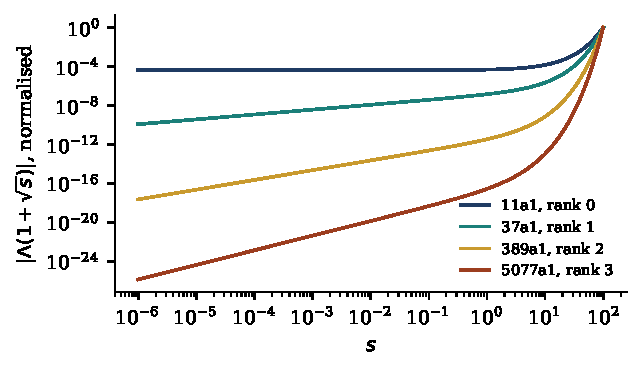
\includegraphics[width=\textwidth]{figs/thorin_rankatom.pdf}
\caption{$|\Lambda(1+\sqrt s,E)|$ on log log axes, normalised to $1$ at $s=100$, for the elliptic curves 11a1, 37a1, 389a1, 5077a1 of ranks $r=0$ to $3$. Near $s=0$ the slopes are $0$, $0.500$, $1.000$, $1.500$: a degenerate Thorin atom of mass $r/2$ at the origin.}\label{fig:10brankatom}
\end{minipage}\hfill
\begin{minipage}[t]{0.48\textwidth}\centering
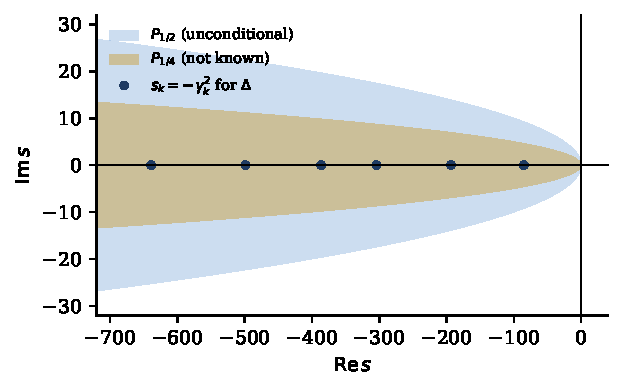
\includegraphics[width=\textwidth]{figs/thorin_parabola10b.pdf}
\caption{The parabolic regions $P_{1/2}$ and $P_{1/4}$ in the plane of $s = z^2$, with the points $s_k = -\gamma_k^2$ for the first six zeros of $\Delta$. For every $\pi$ all $s_k$ lie in $P_{1/2}$ (condition $\Theta_{1/2}$, unconditional); $\Theta_{1/4}$ is known for no $\pi$. GRH puts every $s_k$ on $P_0 = (-\infty,0]$.}\label{fig:10bparabola}
\end{minipage}
\end{figure}

\begin{proposition}[this book]\label{prop:10brank}
Let $\pi\cong\tilde\pi$ with $r = \operatorname{ord}_{s=1/2}\Lambda(s,\pi)\ge1$ and $H(z) = \Lambda(\frac12+z,\pi)/z^r$. Unconditionally,
\[
\lim_{s\to0^+}\frac{d\log|\Lambda(\frac12+\sqrt s,\pi)|}{d\log s} = \frac r2 .
\]
Under GRH for $\pi$, for $s>0$,
\[
\frac{H(0)}{\Lambda(\frac12+\sqrt s,\pi)} = s^{-r/2}\,\E e^{-sX} = \int_0^\infty e^{-sx}\,(m_r*\mu_X)(dx),
\]
with $m_r(dx) = x^{r/2-1}dx/\Gamma(r/2)$, $X$ the GGC of Theorem~\ref{thm:10bmain}(c) for $\Xi^{\mathrm{sd}}_\pi$ and $\mu_X$ its law. The infinite measure $m_r$ is the increasing limit as $\epsilon\downarrow0$ of $\epsilon^{-r/2}$ times the gamma law of shape $r/2$ and rate $\epsilon$, whose Thorin measure is $\frac r2\delta_\epsilon$: a Thorin atom of mass $r/2$ escaping to the origin.
\end{proposition}

\begin{proof}
$\log|\Lambda(\frac12+\sqrt s)| = \frac r2\log s+\log|H(\sqrt s)|$ and $H(\sqrt s)\to H(0)\ne0$ with derivative in $\log s$ tending to zero, which gives the slope. Under GRH, Theorem~\ref{thm:10bmain} gives $H(0)/H(\sqrt s) = \E e^{-sX}$. Also $\int_0^\infty e^{-sx}x^{r/2-1}dx/\Gamma(r/2) = s^{-r/2}$, and the Laplace transform of a convolution of positive measures is the product, by Tonelli. Finally the gamma density of shape $r/2$ and rate $\epsilon$ times $\epsilon^{-r/2}$ is $x^{r/2-1}e^{-\epsilon x}/\Gamma(r/2)$, which increases to the density of $m_r$, and its transform $\epsilon^{-r/2}(1+s/\epsilon)^{-r/2} = (\epsilon+s)^{-r/2}$ tends to $s^{-r/2}$.
\end{proof}

For $r=2$ the density of $m_2*\mu_X$ is $\Prob(X\le x)$. In the product completion $\Xi_\pi$ the central zero has order $2r$ and the degenerate mass is $r$. For an elliptic curve $E/\Q$ the conjecture of Birch and Swinnerton Dyer \cite{bsd1965} identifies the analytic rank with the Mordell Weil rank, so under that conjecture \emph{twice the Thorin mass at the origin of $\Xi^{\mathrm{sd}}$ is the Mordell Weil rank}; for analytic rank at most one this equality is a theorem of Gross and Zagier \cite{grosszagier1986} and Kolyvagin \cite{kolyvagin1988}.\index{Thorin atom at zero}\index{Birch and Swinnerton Dyer conjecture}

Figure~\ref{fig:10brankatom} shows the effect for four curves in the classical normalisation with centre $1$: the slopes of $\log|\Lambda(1+\sqrt s)|$ against $\log s$ between $s = 10^{-6}$ and $10^{-4}$ are $0.500$, $1.000$, $1.500$ for ranks $1$, $2$, $3$ and $0$ for rank $0$, until the atoms $\gamma_k^2$ take over near $s\approx\gamma_1^2$ ($8.27$ for 389a1, $4.21$ for 5077a1).

\section{Parabolic Thorin conditions and the heat flow}\label{sec:10bparabola}

GRH asks that every Thorin atom lie on the half line. A quantitative relaxation asks that they lie in a region around it.

\begin{definition}\label{def:10btheta}
For $\sigma\ge0$, condition $\Theta_\sigma$ for $\pi$ is: every zero $z$ of $\Xi_\pi$ satisfies $|\operatorname{Re}z|\le\sigma$; equivalently every zero of $\Lambda(s,\pi)$ lies in $|\operatorname{Re}s-\frac12|\le\sigma$. Let $P_\sigma = \{x+iy:x\le\sigma^2-y^2/(4\sigma^2)\}$ for $\sigma>0$ and $P_0 = (-\infty,0]$.\index{parabolic Thorin condition}
\end{definition}

\begin{lemma}\label{lem:10bparabola}
For $\sigma\ge0$, $\{z^2:|\operatorname{Re}z|\le\sigma\} = P_\sigma$. Hence $\Theta_\sigma$ holds if and only if every $s_k = z_k^2$ lies in $P_\sigma$, if and only if every Thorin atom $t_k$ lies in $-P_\sigma = \{x+iy:x\ge-\sigma^2+y^2/(4\sigma^2)\}$, the region bounded by the parabola with vertex $-\sigma^2$ that opens along the positive axis. The regions increase with $\sigma$ and $\bigcap_{\sigma>0}(-P_\sigma) = [0,\infty)$.
\end{lemma}

\begin{proof}
The case $\sigma=0$ is $\{(ib)^2\} = (-\infty,0]$. Let $\sigma>0$. The two square roots $\pm w$ of $s = x+iy$ have $|\operatorname{Re}w| = ((|s|+x)/2)^{1/2}$, so $s$ is a square of some $z$ with $|\operatorname{Re}z|\le\sigma$ if and only if $|s|\le2\sigma^2-x$. This requires $x\le2\sigma^2$, and then squaring gives $x^2+y^2\le4\sigma^4-4\sigma^2x+x^2$, that is $x\le\sigma^2-y^2/(4\sigma^2)$; conversely this inequality implies $x\le\sigma^2\le2\sigma^2$. The remaining statements are immediate.
\end{proof}

By Lemma~\ref{lem:10bcompletion}(iii), $\Theta_{1/2}$ holds unconditionally for every $\pi$, with strict inequality: all atoms lie in the interior of $-P_{1/2}$. The image under $z\mapsto z^2$ of the boundary line $\operatorname{Re}z=\frac12$ is the parabola $x = \frac14-y^2$, which is how the nonvanishing theorem of Jacquet and Shalika looks in the $s$ plane. Zero free regions of de la Vall\'ee Poussin type \cite{iwanieckowalski2004} narrow the strip in the $z$ plane by a logarithmically small amount, which in the $s$ plane is a band whose horizontal width grows like $y^2/\log|y|$ (Exercise~\ref{ex:10bzerofree}), but they give $\Theta_\sigma$ for no $\sigma<\frac12$, and for no automorphic $L$ function is $\Theta_\sigma$ known with $\sigma<\frac12$. Condition $\Theta_0$ is GRH (Figure~\ref{fig:10bparabola}).

\subsection{Gaussian tilting}

The P\'olya kernel of Lemma~\ref{lem:10bkernel} can be tilted by a Gaussian factor. For $\lambda\in\R$ put
\[
H_{\pi,\lambda}(t) = \int_{-\infty}^\infty e^{\lambda u^2}\Phi_\pi(u)e^{itu}\,du,
\]
an entire function of $t$, with $H_{\pi,0}(t) = \Xi_\pi(it)/\Xi_\pi(0)$, so $\Theta_\sigma$ says exactly that the zeros of $H_{\pi,0}$ lie in $|\operatorname{Im}t|\le\sigma$. We use de Bruijn's theorem \cite{debruijn1950} in the following form: if $\Phi$ is real, even and integrable with $\Phi(u) = O(\exp(-|u|^{2+\delta}))$ for some $\delta>0$, and all zeros of $H_0(t) = \int\Phi(u)e^{itu}du$ lie in $|\operatorname{Im}t|\le b_0$, then for $\lambda>0$ all zeros of $H_\lambda(t) = \int e^{\lambda u^2}\Phi(u)e^{itu}du$ lie in $|\operatorname{Im}t|\le(\max(b_0^2-2\lambda,0))^{1/2}$. Positivity of $\Phi$ is not needed; see \cite{debruijn1950,newman1976} for the precise hypotheses. By Lemma~\ref{lem:10bkernel} they hold for every $\Phi_\pi$, in particular for $\Delta$ and every multiplicative eta product, and P\'olya's kernel for $\zeta$ satisfies them as well (Chapter~\ref{ch:10}).\index{de Bruijn Newman constant}

\begin{theorem}[Gaussian tilting; (i) de Bruijn, (ii) this book]\label{thm:10btilting}
Suppose $\Theta_\sigma$ holds for $\pi$, and let $\lambda\ge0$.
\begin{enumerate}
\item[(i)] The zeros of $H_{\pi,\lambda}$ lie in $|\operatorname{Im}t|\le\sigma_\lambda$, where $\sigma_\lambda = (\max(\sigma^2-2\lambda,0))^{1/2}$; Gaussian tilting moves the Thorin atoms from $-P_\sigma$ into $-P_{\sigma_\lambda}$, and for $\lambda\ge\sigma^2/2$ all zeros of $H_{\pi,\lambda}$ are real.
\item[(ii)] If $\Phi_\pi\ge0$, let $W_{\pi,\lambda}$ have density proportional to $e^{\lambda u^2}\Phi_\pi(u)$. For every $\lambda\ge\sigma^2/2$ the function $s\mapsto H_{\pi,\lambda}(0)/H_{\pi,\lambda}(i\sqrt s) = 1/\E e^{\sqrt sW_{\pi,\lambda}}$ is the Laplace transform of a GGC with drift zero and Thorin measure $\sum_k\delta_{x_k(\lambda)^2}$, where $\pm x_k(\lambda)$ are the real zeros of $H_{\pi,\lambda}$.
\end{enumerate}
Unconditionally ($\sigma=\frac12$), $H_{\pi,\lambda}$ has only real zeros for every $\lambda\ge\frac18$, and (ii) holds for these $\lambda$.
\end{theorem}

\begin{proof}
(i) is de Bruijn's theorem with $b_0 = \sigma$, translated by Lemma~\ref{lem:10bparabola}. For (ii), $E_\lambda(z) = H_{\pi,\lambda}(-iz)/H_{\pi,\lambda}(0) = \E e^{zW_{\pi,\lambda}}$ is well defined because $H_{\pi,\lambda}(0) = \int e^{\lambda u^2}\Phi_\pi>0$, even because $\Phi_\pi$ is even, real on $\R$, and $E_\lambda(0)=1$. Its order is at most one: with $|\Phi_\pi(u)|\le C\exp(-ce^{c|u|})$ one has $\sup_u(\lambda u^2+|z||u|-\frac c2e^{c|u|}) = O(|z|\log(|z|+2))$. By (i) its zeros $z = ix_k(\lambda)$ lie on $i\R$, so Theorem~\ref{thm:10babstract}, (a) implies (c), applies with $\sigma_0=0$. The unconditional case is $\sigma=\frac12$, from Lemma~\ref{lem:10bcompletion}(iii).
\end{proof}

\begin{remark}[The factor four]
The literature normalisation for $\zeta$ (Chapter~\ref{ch:10}) is $H^{\mathrm{cl}}_0(x) = \frac18\Xi(x/2)$, $\Xi(t) = \xi(\frac12+it)$, with kernel tilt $e^{\lambda_{\mathrm{cl}}v^2}$. Since $t = x/2$, the kernel variables satisfy $u = 2v$, so $e^{\lambda_{\mathrm{cl}}v^2} = e^{(\lambda_{\mathrm{cl}}/4)u^2}$ and $\lambda = \lambda_{\mathrm{cl}}/4$. De Bruijn's classical bound $\lambda_{\mathrm{cl}}\ge\frac12$, from zeros of $H^{\mathrm{cl}}_0$ in $|\operatorname{Im}x|<1$, is our $\lambda\ge\frac18$, from zeros of $H_0$ in $|\operatorname{Im}t|<\frac12$; the Polymath bound $\Lambda\le0.22$ \cite{polymath2019} is $0.055$ in our units.
\end{remark}

Define the de Bruijn Newman constant $\lambda_\pi\in[-\infty,\frac18]$ of $\pi$, in our units, as the infimum of the $\lambda$ for which $H_{\pi,\lambda}$ has only real zeros. If $H_{\pi,\lambda_0}$ has only real zeros, de Bruijn's theorem applied to the kernel $e^{\lambda_0u^2}\Phi_\pi$ with $b_0=0$ shows that $H_{\pi,\lambda}$ has only real zeros for every $\lambda>\lambda_0$. The set of such $\lambda$ is also closed, by Hurwitz's theorem, so it is $[\lambda_\pi,\infty)$ when $\lambda_\pi$ is finite, and GRH for $\pi$ is equivalent to $\lambda_\pi\le0$. When $\Phi_\pi\ge0$, Theorem~\ref{thm:10babstract} (whose equivalence of (a) and (b) needs no strip hypothesis; see the paragraph after its proof) identifies this set with the set of $\lambda$ for which the tilted reciprocal is a GGC transform: \emph{the Thorin property holds exactly on $[\lambda_\pi,\infty)$}. Rodgers and Tao \cite{rodgerstao2020} proved Newman's conjecture $\lambda_\zeta\ge0$, and Dobner's extension \cite{dobner2021} to the extended Selberg class gives $\lambda_\Delta\ge0$, as Chapter~\ref{ch:10} explains; we expect, but do not verify here, that it gives $\lambda_\pi\ge0$ for the other kernels $\Phi_\pi$ of this chapter. For $\zeta$, and for every $\pi$ with $\Phi_\pi\ge0$ and $\lambda_\pi\ge0$, GRH would therefore mean $\lambda_\pi=0$: the tilted reciprocal is a GGC transform for every $\lambda\ge0$ and for no $\lambda<0$. \emph{For such $\pi$, if GRH holds, $1/F_\pi$ lies exactly on the edge of the class of GGC transforms along the heat flow}, in line with Newman's remark that the Riemann hypothesis, if true, is only barely so.

\begin{proposition}[Motion of Thorin atoms]\label{prop:10bflow}
Let $I$ be an open interval of $\lambda$ on which $H_{\pi,\lambda}(0)\ne0$ and all zeros of $H_{\pi,\lambda}$ are real and simple, written $\pm x_k(\lambda)$, $x_k>0$, and let $t_k(\lambda) = x_k(\lambda)^2$. Then each $t_k$ is real analytic on $I$ and
\[
\frac{dt_k}{d\lambda} = 2+8\sum_{j\ne k}\frac{t_k}{t_k-t_j},
\]
the series converging absolutely.
\end{proposition}

\begin{proof}
$H(t,\lambda) = H_{\pi,\lambda}(t)$ is jointly analytic, and differentiating under the integral gives $\partial_\lambda H = -\partial_t^2H$. At a simple zero the implicit function theorem gives analytic $x_k(\lambda)$ with $x_k' = -\partial_\lambda H/\partial_tH = H''(x_k)/H'(x_k)$, primes on $H$ denoting $t$ derivatives. As in the proof of Theorem~\ref{thm:10btilting}, $H_{\pi,\lambda}(t) = H_{\pi,\lambda}(0)(1-t^2/t_k)g(t)$ with $g(t) = \prod_{j\ne k}(1-t^2/t_j)$, locally uniformly convergent. Writing $H = (t-x_k)q(t)$ with $q(t) = -H_{\pi,\lambda}(0)t_k^{-1}(t+x_k)g(t)$ and $q(x_k)\ne0$, we get $H'(x_k) = q(x_k)$ and $H''(x_k) = 2q'(x_k)$, and $g'/g(t) = \sum_{j\ne k}2t/(t^2-t_j)$, so
\[
x_k' = 2\Bigl(\frac1{2x_k}+\sum_{j\ne k}\frac{2x_k}{x_k^2-x_j^2}\Bigr).
\]
Multiplying by $2x_k$ gives the formula. Absolute convergence follows from $|t_k/(t_k-t_j)|\le2t_k/t_j$ for large $j$ and $\sum_jt_j^{-1}<\infty$.
\end{proof}

The constant $2$ is the repulsion of each zero from its mirror image. In the variable $x$ the flow is the classical zero dynamics of the backward heat equation, $x_k' = 2\sum(x_k-x)^{-1}$ over all other zeros $x$, summed symmetrically, and formally $x_k'' = -8\sum(x_k-x)^{-3}$, an inverse cube interaction of Calogero Moser type; the proposition only rewrites it for the Thorin atoms $t_k = x_k^2$. As $\lambda$ decreases the atoms attract; heuristically, a collision is the moment two real zeros meet and leave the axis as a conjugate pair, and $\lambda_\pi$ is the supremum of the collision times. Csordas, Smith and Varga \cite{csordassmithvarga1994} obtained lower bounds for $\lambda_\zeta$ from close pairs of zeros along these lines. We use the dynamics only heuristically; continuation through collisions is not addressed.

\section{A catalogue of applications}

The proof of Theorem~\ref{thm:10bmain} uses only that $\Lambda$ is entire of order one, satisfies a functional equation relating it to its conjugate, and is zero free off the strip $0<\operatorname{Re}s<1$. This is known in the following cases.\index{automorphic $L$ function}

\emph{Dirichlet $L$ functions.} For primitive $\chi\ne1$, $\Lambda(s,\chi)$ is entire; real $\chi$ are self dual, and for complex $\chi$, $\Xi_\chi(x) = |\Lambda(\frac12+x,\chi)|^2/x^{2r}$ on $\R$.

\emph{Dedekind and Hecke $L$ functions.} For a number field $K$, $s(s-1)\Lambda_K(s)$ is entire and symmetric under $s\mapsto1-s$; Hecke $L$ functions of nontrivial Gr\"o{\ss}encharaktere are entire \cite{hecke1918,tate1967}.

\emph{Newforms and elliptic curves.} For a holomorphic newform $f$, $\Lambda(s,f)$ is entire \cite{hecke1937,atkinlehner1970}; by modularity \cite{wiles1995,taylorwiles1995,bcdt2001} this covers every elliptic curve over $\Q$.

\emph{Symmetric powers.} Newton and Thorne \cite{newtonthorne2021,newtonthorne2021b} proved that for every holomorphic newform $f$ of weight at least two without complex multiplication, $\Sym^m\pi_f$ is a cuspidal automorphic representation of $\GL_{m+1}(\A_\Q)$ for every $m\ge1$. Hence Theorem~\ref{thm:10bmain} applies to every symmetric power of every such form. (With complex multiplication $\Sym^mf$ splits into Hecke characters, and for $4\mid m$ a trivial constituent gives a pole, removed as for $\zeta$.)

\emph{Rankin Selberg $L$ functions.} For cuspidal $\pi,\pi'$ with $\pi'\not\cong\tilde\pi$, $\Lambda(s,\pi\times\pi')$ is entire with a functional equation \cite{jpss1983,moeglinwaldspurger1989}, bounded in vertical strips away from the real axis by Gelbart and Shahidi \cite{gelbartshahidi2001}, which gives order one, and nonzero on $\operatorname{Re}s=1$ by Shahidi \cite{shahidi1981}. For $\pi' = \tilde\pi$ there are simple poles at $s=0,1$, removed by the factor $s(s-1)$. Theorem~\ref{thm:10babstract} applies with the same proof.

\emph{Artin $L$ functions.} The theorem applies to every irreducible $\rho$ for which Artin's conjecture is known. By Khare and Wintenberger \cite{kharewintenberger2009} every odd irreducible two dimensional $\rho$ comes from a weight one newform, so this includes all of them. Our example is the representation of $S_3$ cut out by $x^3-x-1$, of conductor $23$, with $L$ function $\zeta_K(s)/\zeta(s)$ for the cubic field $K$, the $L$ function of $\eta(\tau)\eta(23\tau)$.

\begin{table}[t]
\centering
\footnotesize
\setlength{\tabcolsep}{3.2pt}
\begin{tabular}{lrrrrrrrc}
\toprule
$L$ function & $d$ & $N$ & $r$ & $\gamma_1$ & $S_1$ Taylor & $S_1$ zeros & err$(25)$ & Hankel\\
\midrule
$\zeta$ (via $\xi$) & 1 & 1 & 0 & 14.1347 & 0.023105 & 0.023108 & $8.3\cdot10^{-5}$ & yes\\
$L(s,\chi_{-4})$ & 1 & 4 & 0 & 6.0209 & 0.078015 & 0.078013 & $3.9\cdot10^{-5}$ & yes\\
$L(s,\chi_{-3})$ & 1 & 3 & 0 & 8.0397 & 0.056701 & 0.056696 & $1.1\cdot10^{-4}$ & yes\\
$L(s,\chi_5)$ & 1 & 5 & 0 & 6.6485 & 0.078457 & 0.078462 & $1.3\cdot10^{-4}$ & yes\\
$\Delta$ & 2 & 1 & 0 & 9.2224 & 0.0561759 & 0.0561824 & $1.7\cdot10^{-4}$ & yes\\
11a1 & 2 & 11 & 0 & 6.3626 & 0.127589 & 0.127584 & $1.1\cdot10^{-4}$ & yes\\
37a1 & 2 & 37 & 1 & 5.0032 & 0.189609 & 0.189611 & $5.4\cdot10^{-5}$ & yes\\
389a1 & 2 & 389 & 2 & 2.8761 & 0.407048 & 0.407051 & $1.0\cdot10^{-4}$ & yes\\
5077a1 & 2 & 5077 & 3 & 2.0525 & 0.725919 & 0.725921 & $6.0\cdot10^{-5}$ & yes\\
Artin, $x^3-x-1$ & 2 & 23 & 0 & 5.1157 & 0.170287 & 0.170294 & $1.8\cdot10^{-4}$ & yes\\
$\Sym^2$ 11a1 & 3 & 121 & 0 & 3.8993 & 0.321206 & 0.321205 & $2.1\cdot10^{-5}$ & yes\\
\bottomrule
\end{tabular}
\caption{The global Thorin catalogue, computed with $\Xi^{\mathrm{sd}}$: degree $d$, conductor $N$, central order $r$, first ordinate $\gamma_1$ beyond the centre, $S_1 = \sum\gamma_k^{-2}$ from central Taylor coefficients and from the zeros to height $300$ plus the tail estimate, absolute relative error of the product formula at $s=25$, and positivity of $\det(S_{i+j+1})_{m\times m}$, $m\le4$, and $\det(S_{i+j+2})_{m\times m}$, $m\le3$, computed from Taylor coefficients alone.}\label{tab:10bcatalogue}
\end{table}

Table~\ref{tab:10bcatalogue} records computations carried out for this book on eleven self dual $L$ functions, using $\Xi^{\mathrm{sd}}$. We computed the zeros to height $T = 300$ ($138$ to $680$ of them) and compared $\Xi^{\mathrm{sd}}(\sqrt s)/\Xi^{\mathrm{sd}}(0)$ with $\prod(1+s/\gamma_k^2)\exp(s\sum_{\gamma>T}\gamma^{-2})$, the tail estimated by $(\log N+d\log(T/2\pi)+d)/(2\pi T)$, which is the integral of $t^{-2}$ against the zero density $(\log N+d\log(t/2\pi))/(2\pi)$ over $t>T$. The relative error is at most $2.8\cdot10^{-5}$ at $s=4$, $1.8\cdot10^{-4}$ at $s=25$ and $8\cdot10^{-4}$ at $s=100$ in every case. The same tail estimate is added to $S_1$ from zeros in the table. For $S_3$ and $S_4$ the values from Taylor coefficients and from zeros agree to all printed digits, for instance $1.8373\cdot10^{-6}$ and $2.0017\cdot10^{-8}$ for $\Delta$, $1.4417\cdot10^{-7}$ and $6.6303\cdot10^{-10}$ for $\zeta$. For $S_2$ the zero sums carry no tail correction and fall short of the Taylor values ($1.9975\cdot10^{-4}$ for $\Delta$, $3.7173\cdot10^{-5}$ for $\zeta$) by the omitted tail $\sum_{\gamma>T}\gamma^{-4}$, a relative amount of at most $2.2\cdot10^{-4}$. The coefficients of $\log F(s)$ alternate in sign through $n=8$ for all eleven functions, as GRH requires (Remark~\ref{rem:10bfinite}). The Hankel determinants $\det(S_{i+j+1})_{m\times m}$, $m\le4$, and $\det(S_{i+j+2})_{m\times m}$, $m\le3$, computed from central Taylor coefficients at $60$ digit precision without using any zero, are positive in every case; for $\Delta$ the first family is $5.618\cdot10^{-2}$, $6.331\cdot10^{-8}$, $4.749\cdot10^{-19}$, $9.579\cdot10^{-36}$, and for $\zeta$ it is $2.310\cdot10^{-2}$, $1.949\cdot10^{-9}$, $2.173\cdot10^{-22}$, $1.178\cdot10^{-41}$. These are necessary conditions for GRH, so the computation is consistent with it; by Remark~\ref{rem:10bfinite} it constrains only the lowest atoms.

\section{The Thorin threshold}

Everything above requires $\sum_k|t_k|^{-1}<\infty$, which makes $F$ a genus zero product and $\sum E_k/t_k$ convergent; for automorphic $L$ functions $N(T)\asymp T\log T$ gives it with room to spare. The Selberg zeta function crosses this threshold.\index{Thorin threshold}

Let $\Gamma\backslash\mathbb H$ be a compact hyperbolic surface with Laplace eigenvalues $0 = \lambda_0<\lambda_1\le\lambda_2\le\dots$ and write $\lambda_j = \frac14+r_j^2$. Selberg's zeta function $Z_\Gamma(s)$ \cite{selberg1956,hejhal1976} has zeros at $s = \frac12\pm ir_j$, and by Sarnak \cite{sarnak1987b} it equals, up to an explicit factor built from the Barnes double gamma function, the regularised determinant $\det(\Delta_\Gamma-s(1-s))$. Removing the zeros at $s=0,1$ from $\lambda_0 = 0$ and assuming for simplicity that $\frac14$ is not an eigenvalue, we obtain an even entire $E_\Gamma(z)$, real on $\R$, $E_\Gamma(0) = 1$, with zeros $\pm ir_j$, $j\ge1$, and put $F_\Gamma(s) = E_\Gamma(\sqrt s)$. Its Thorin atoms are
\[
t_j = r_j^2 = \lambda_j-\tfrac14,
\]
the spectrum of $\Delta_\Gamma-\frac14$. But Weyl's law $\#\{j:\lambda_j\le x\}\sim\frac{\operatorname{area}}{4\pi}x$ \cite{weyl1912,hejhal1976} gives $\#\{j:|r_j|\le T\}\sim\frac{\operatorname{area}}{4\pi}T^2$, so $E_\Gamma$ has order two, $\sum_j|t_j|^{-1}$ diverges logarithmically and $\sum_j|t_j|^{-2}<\infty$. The reciprocal is no longer a GGC transform even when all $t_j>0$, but a compensated version survives.

\begin{proposition}[Regularised Thorin equivalence; this book]\label{prop:10bregularised}
Let $E$ be entire, even, real on $\R$, $E(0)=1$, of order at most two with zeros $\pm z_k$ satisfying $\sum|z_k|^{-4}<\infty$, and let $t_k = -z_k^2$, $F(s) = E(\sqrt s)$. Then $F(s) = e^{bs}\prod_k(1+s/t_k)e^{-s/t_k}$ for some real $b$, and the following are equivalent: (a) all $t_k>0$; (b) for independent standard exponential variables $E_k$ the series $Y = b+\sum_k(E_k-1)/t_k$, which converges in $L^2$, is real valued and satisfies $1/F(s) = \E e^{-sY}$ for $s\ge0$; (c) $1/F$ agrees on $(0,\infty)$ with a function holomorphic and zero free on $\C\setminus(-\infty,0]$. The law of $Y$ in (b) is infinitely divisible with L\'evy measure $x^{-1}\sum_ke^{-t_kx}dx$ on $(0,\infty)$; when $\sum_kt_k^{-1} = \infty$ its first moment $\int_0^1\sum_ke^{-t_kx}dx$ near the origin is infinite, which is why the centring is needed.
\end{proposition}

\begin{proof}
$F$ has order at most one with $\sum|t_k|^{-2}<\infty$, so Hadamard's theorem gives the genus one product with a factor $e^{a+bs}$, $a = 0$ since $F(0)=1$; $b$ is real since $\{t_k\}$ is closed under conjugation and $F$ is real on $(0,\infty)$. The series for $Y$ converges in $L^2$ because its summands are independent with mean zero and $\sum_k|t_k|^{-2}<\infty$. (a) implies (b): if all $t_k>0$ the series also converges almost surely, and $\E e^{-s(E_k-1)/t_k} = e^{s/t_k}(1+s/t_k)^{-1}$. For fixed $s\ge0$ the normalised partial products $e^{-sY_N}/\E e^{-sY_N}$, with $Y_N = \sum_{k\le N}(E_k-1)/t_k$, form a positive martingale whose second moments are $\prod_{k\le N}(1+s/t_k)^2(1+2s/t_k)^{-1}\le\prod_k(1+s^2/t_k^2)<\infty$; it is therefore uniformly integrable, and passing to the limit gives (b). (b) implies (a): the imaginary part of $Y$ is $\sum_k\operatorname{Im}(t_k^{-1})(E_k-1)$, a sum of independent variables that has a continuous law as soon as one coefficient is nonzero, so $Y$ real forces every $t_k$ real; and a real $t_k<0$ would make $\E e^{-s(E_k-1)/t_k}$, hence $\E e^{-sY}$, infinite for every $s\ge|t_k|$, while $1/F$ is finite on $(0,\infty)$ outside a discrete set. (a) implies (c): each factor $e^{s/t_k}(1+s/t_k)^{-1}$ is holomorphic and zero free on $\C\setminus(-\infty,0]$ and the product converges locally uniformly there. (c) implies (a): the identity theorem shows that $F$ has no zeros off $(-\infty,0]$, and $F(0) = 1$, so all $t_k>0$. The L\'evy measure follows from Frullani's integral applied to each factor.
\end{proof}

For the surface, (a) says $\lambda_1\ge\frac14$ (strictly, under our simplifying assumption): the Thorin property of the regularised reciprocal of the Selberg zeta function is the absence of exceptional eigenvalues. On a general surface small eigenvalues give negative atoms $t_j\in(-\frac14,0)$. For arithmetic surfaces this is Selberg's eigenvalue conjecture \cite{selberg1965}, for congruence subgroups of $\SL_2(\Z)$ and, through the Jacquet Langlands correspondence \cite{jacquetlanglands1970}, for the compact quaternion surfaces over $\Q$. There the bound $\lambda_1\ge\frac{975}{4096} = \frac14-(\frac7{64})^2$ of Kim and Sarnak \cite{kimsarnak2003} says precisely that every atom satisfies $t_j\ge-(\frac7{64})^2$: condition $\Theta_{7/64}$ for the spectral zeros. (For noncompact congruence surfaces the zeros from the scattering determinant must first be separated.) In field theoretic terms, if all $t_j>0$ then $\sum_jE_j/t_j$ is the formal squared norm of the complex Gaussian field with covariance $(\Delta_\Gamma-\frac14)^{-1}$, and the centring in $Y$ is its Wick renormalisation, needed because that norm diverges logarithmically in two dimensions.

\begin{problem}[Selberg's conjecture as a regularised Thorin problem]
For the family of compact arithmetic surfaces attached to maximal orders in indefinite quaternion algebras over $\Q$, or for congruence surfaces after removal of the scattering zeros, construct directly, without spectral input and uniformly in the level, real random variables $Y_\Gamma$ with $\E e^{-sY_\Gamma} = 1/F_\Gamma(s)$ for every $s\ge0$; under (a) of Proposition~\ref{prop:10bregularised} the variable of its part (b) is one. Since the atoms $t_j = \lambda_j-\frac14$ are real, a negative atom would make $1/F_\Gamma$ infinite at the point $s = -t_j>0$ but finite at $0$ and at all large $s$, which is impossible for a Laplace transform, whose domain of finiteness is an interval. Such a construction would therefore prove Selberg's eigenvalue conjecture for the family. More modestly, develop the Thorin theory of order two: the analogues of the L\'evy function criterion and of the Hankel criterion, Theorem~\ref{thm:10babstract}(d) and (f), for compensated sums.
\end{problem}

\section{Pictures of the Thorin property}
Figures~\ref{fig:10bphase} and \ref{fig:10bthorin} show the two sides of Theorem~\ref{thm:10bmain} for $\Delta$. The phase portrait of $\Lambda(6+z,\Delta)$ (classical normalisation, centre $6$) colours each point by the argument of the function, with brightness bands for its modulus; a zero is a point where every colour meets. In the window every zero lies on the axis $\mathrm{Re}\,z=0$, as the Riemann hypothesis for $\Delta$ predicts; this is a numerical observation, not a proof. Since $\Lambda(6+z,\Delta)$ is even in $z$, the reciprocal $\Lambda(6)/\Lambda(6+\sqrt s)$ is meromorphic in the whole plane of $s=z^2$, and in the window its only poles are the points $-\gamma_k^2$ on the negative axis: this is the analytic shape of a generalized gamma convolution whose Thorin measure is $\sum_k\delta_{\gamma_k^2}$.

\begin{figure}[ht]\centering
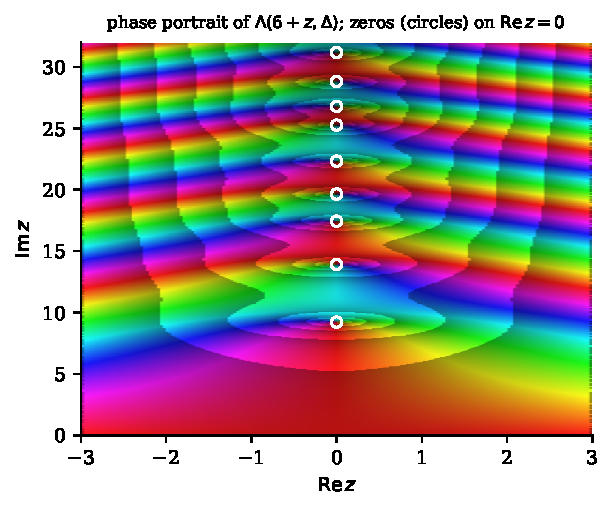
\includegraphics[width=0.92\textwidth]{figs/domain_delta.pdf}
\caption{Phase portrait of $\Lambda(6+z,\Delta)$ for $|\mathrm{Re}\,z|\le3$, $0\le\mathrm{Im}\,z\le32$, with the modulus normalised along each horizontal line. The white circles mark the zeros found on $\mathrm{Re}\,z=0$ by PARI/GP; the colours show no other zero in the window.}\label{fig:10bphase}
\end{figure}

\begin{figure}[ht]\centering
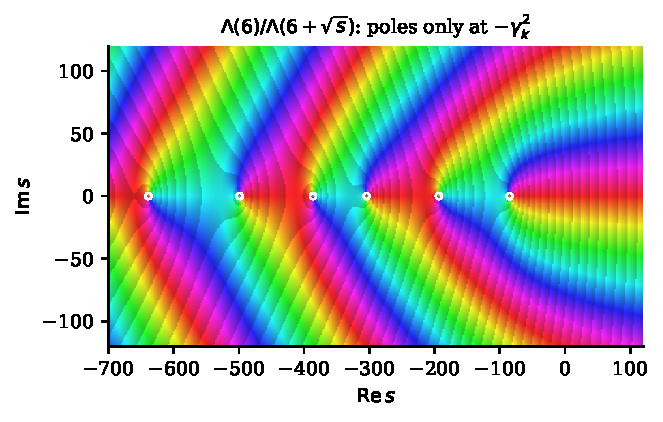
\includegraphics[width=0.95\textwidth]{figs/domain_thorin.pdf}
\caption{Domain colouring of $\Lambda(6,\Delta)/\Lambda(6+\sqrt s,\Delta)$ in the $s$ plane. The circles mark $-\gamma_k^2$ for the first six zeros of $\Delta$; the colour wheel winds around each of them with the orientation of a pole, and around no other point of the window.}\label{fig:10bthorin}
\end{figure}

\section{Notes}

For generalized gamma convolutions, the reciprocal $\Xi$ function, the Brownian reading of $\xi$ and the heat flow see the Notes to Chapter~\ref{ch:10}. Bernstein's theorem is \cite{bernstein1929}; Stieltjes functions and their Nevanlinna Pick characterisation are treated in \cite{schillingsongvondracek2012}, and the moment problem on the half line in \cite{stieltjes1894,akhiezer1965}. The equivalence of (a), (b) and (c) of Theorem~\ref{thm:10babstract} for Laguerre P\'olya functions, with its van Dantzig and Wald forms, is from \cite{polson2018vdp}. As far as we know, the self dual completion for general $\pi$, the forms (d), (e) and (f) in this generality, the cumulant criterion, the rank atom, the parabolic and tilted versions and the computations have not appeared in this form, although each rests on classical ingredients: Hankel criteria for real zeros go back to Hermite and Grommer \cite{grommer1914}, and Newton's identities link the power sums $S_n$ to the central Taylor coefficients. The results labelled as ours are elementary consequences of Hadamard's factorisation, the identity theorem and the classical facts cited; none proves a Riemann hypothesis. The zero dynamics under the heat flow, which Proposition~\ref{prop:10bflow} rewrites for the Thorin atoms, were used by Csordas, Smith and Varga \cite{csordassmithvarga1994} and by the Polymath project \cite{polymath2019}. Numerical values were computed for this book with PARI/GP \cite{pari2023}; the first zeros agree with those listed in the LMFDB \cite{lmfdb}.

\section{Exercises}

\begin{enumerate}
\item Let $g(s) = \sum_{j=1}^Jc_j/(s+t_j)$ with $c_j>0$ and distinct real $t_j$. Show directly that $\operatorname{Im}g(s)\le0$ on the upper half plane, and that $g$ is a Stieltjes function if and only if every $t_j\ge0$. Show that if the $t_j$ may be complex, closed under conjugation with equal weights on conjugate pairs, then $\operatorname{Im}g\le0$ on the upper half plane forces all $t_j$ real.
\item For $\nu>-1$ let $E_\nu(z) = \Gamma(\nu+1)(2/z)^\nu I_\nu(z)$, whose zeros are $\pm ij_{\nu,k}$ with $j_{\nu,k}>0$ the zeros of $J_\nu$. Show that $E_\nu$ satisfies the hypotheses of Theorem~\ref{thm:10babstract}, that $S_1 = \frac1{4(\nu+1)}$ and $S_2 = \frac1{16(\nu+1)^2(\nu+2)}$, and check the case $\nu = \frac12$, $E(z) = \sinh z/z$, against $\sum(\pi k)^{-2} = \frac16$ and $\sum(\pi k)^{-4} = \frac1{90}$. Compute $S_3$ and $S_4$ by Corollary~\ref{cor:10bnewton} and verify that the two $2\times2$ Hankel determinants $S_1S_3-S_2^2$ and $S_2S_4-S_3^2$ are positive.
\item\label{ex:10bzerofree} Verify Lemma~\ref{lem:10bparabola} by showing that $z\mapsto z^2$ maps the line $\operatorname{Re}z = a>0$ onto the parabola $x = a^2-y^2/(4a^2)$. Show that the image of the curve $\operatorname{Re}z = \frac12-c/\log(|\operatorname{Im}z|+3)$ lies at horizontal distance asymptotic to $4cy^2/\log|y|$ from the parabola $x = \frac14-y^2$ as $|y|\to\infty$: a zero free region that is logarithmically thin in the $z$ plane is a wide region in the $s$ plane.
\item Let $E/\Q$ have analytic rank $2$, assume GRH for $E$, and put $H(z) = \Lambda(1+z,E)/z^2$. Show that $H(0)/\Lambda(1+\sqrt s,E) = \int_0^\infty e^{-sx}\Prob(X\le x)\,dx$ with $X$ the GGC of Proposition~\ref{prop:10brank}, and deduce that $s\mapsto H(0)/\Lambda(1+\sqrt s,E)$ is completely monotone on $(0,\infty)$. For rank $3$ find the corresponding fractional integral.
\item Let $W$ be the P\'olya variable of $\zeta$. Using Proposition~\ref{prop:10bcumulants} and $S_1 = 0.023105$, $S_2 = 3.7173\cdot10^{-5}$, compute the variance and the excess kurtosis $\kappa_4/\kappa_2^2 = -3S_2/S_1^2$ of $W$. Prove that $-3S_2/S_1^2\in(-3,0)$ whenever all $t_k>0$ and there are at least two atoms, and show by an example with one conjugate pair of nonreal atoms that $-3S_2/S_1^2$ can then be positive.
\end{enumerate}

\section{Open computational problems}

\begin{compproblem}[Certified Thorin Hankel determinants]
Objective: certify the positivity of the Hankel determinants $\det(S_{i+j+1})_{m\times m}$ and $\det(S_{i+j+2})_{m\times m}$ for $m\le20$, computed from central derivatives only. Objects and scale: all $L$ functions in LMFDB of degree at most $4$ and analytic conductor below $10^3$. Route: central derivatives $\Xi^{(2j)}(0)$, $2j\le80$, in rigorous ball arithmetic (Arb, cross checked with PARI/GP \texttt{lfun}), Corollary~\ref{cor:10bnewton} in interval arithmetic, and interval Cholesky factorisation; the precision needed grows roughly like $m^2\log t_m$ digits. Deliverable: a table of certified lower bounds for the smallest eigenvalue of each Hankel matrix, and the smallest $m$ at which certification fails for lack of precision. Why it matters: these are the finite sections of the Thorin Hankel criterion, Theorem~\ref{thm:10bmain}(f), and the margins quantify how the criterion sees the lowest atoms (Remark~\ref{rem:10bfinite}).
\end{compproblem}

\begin{compproblem}[The Herglotz test in the upper half plane]
Objective: map $\operatorname{Im}(F'/F)(s)$ on a grid in $\{\operatorname{Im}s>0\}$ and measure its distance from violating Theorem~\ref{thm:10bmain}(e). Objects and scale: the eleven functions of Table~\ref{tab:10bcatalogue} and all elliptic curves of conductor below $10^4$, on a logarithmic grid with $\operatorname{Re}s\in[-10^4,10^2]$, $\operatorname{Im}s\in[10^{-3},10^3]$, about $10^6$ points each; on the lines $\operatorname{Im}s=\varepsilon$ the map gives, up to a constant factor and the change of variable $z=-\operatorname{Re}s$, the signed densities $u_\varepsilon$ of Chapter~\ref{ch:scholze}. Route: $\Lambda$ and $\Lambda'$ at $\frac12+\sqrt s$ with PARI/GP \texttt{lfunlambda}, parallelised over grid points. Deliverable: heat maps of $-\operatorname{Im}(F'/F)\cdot|s|$, the minimum over the grid, and an empirical law for how the minimum decays as the grid approaches the negative axis. Why it matters: an off line zero $z_0$ of $\Xi$ would give a pole of $F'/F$ at $s_0 = z_0^2$, with $\operatorname{Im}s_0 = 2|\operatorname{Re}z_0\operatorname{Im}z_0|$, surrounded by a region where $\operatorname{Im}(F'/F)>0$; the computation calibrates how such a region would be seen.
\end{compproblem}

\begin{compproblem}[Collision times of the Thorin atoms of $\Delta$]
Objective: measure how close the low zeros of $\Delta$ are to leaving the critical line under the backward heat flow. Let $\lambda_c(K)<0$ be the first collision time of the truncated system in which the lowest $K$ atoms $\gamma_k^2$ move from $\lambda = 0$ downwards by the equation of Proposition~\ref{prop:10bflow}, the atoms beyond them being replaced in the interaction sum, from $\gamma_{K+1}$ on, by their fixed smooth density $\frac1\pi\log\frac{\gamma}{2\pi}$ in the ordinate $\gamma$; the atoms are those of the self dual kernel $\Phi^{\mathrm{sd}}_\Delta$, since the proposition needs simple zeros and for the product kernel $\Phi^{\mathrm{sd}}_\Delta*\Phi^{\mathrm{sd}}_\Delta$ every atom is double. Objects and scale: $K$ from $10$ to $10^5$, hence the first $10^5$ zeros of $L(s,\Delta)$, and $\lambda\in[-1,0]$. Route: zeros by PARI/GP \texttt{lfunzeros}, an adaptive implicit integrator with fast multipole summation, validated for small $|\lambda|$ against the zeros of $t\mapsto\int e^{\lambda u^2}\Phi^{\mathrm{sd}}_\Delta(u)\cos(tu)\,du$ located by quadrature. Deliverable: $\lambda_c(K)$ on a grid of $K$, the pair responsible (a Lehmer pair for $\Delta$), and the dependence of $\lambda_c(K)$ on $K$. Why it matters: since $\lambda_\Delta\ge0$ (Chapter~\ref{ch:10}), the Riemann hypothesis for $\Delta$ would make the Thorin property hold exactly for $\lambda\ge0$ (Theorem~\ref{thm:10btilting} and the discussion after it) and, heuristically, $0$ the supremum of the collision times; $\lambda_c(K)$ measures how narrowly the hypothesis would hold among the lowest $K$ atoms.
\end{compproblem}

\begin{compproblem}[A regularised Thorin computation for a Selberg zeta function]
Objective: test Proposition~\ref{prop:10bregularised} numerically for an arithmetic surface. Objects and scale: the first $10^4$ Laplace eigenvalues of the compact quotient $\Gamma\backslash\mathbb H$, with $\Gamma$ the norm one units of a maximal order in the quaternion algebra of discriminant $6$ over $\Q$ (an orbifold of genus $0$), and of the modular surface (Maass cusp forms, scattering part separated). Route: eigenvalues by Hejhal's method or finite elements, checked against the trace formula and Weyl's law; the law of $Y = b+\sum_j(E_j-1)/t_j$ by Monte Carlo with $10^6$ draws and the Weyl tail added as a Gaussian correction. Deliverable: the atoms $t_j = \lambda_j-\frac14$, a plot of the L\'evy function $\sum_je^{-t_jx}$ against its Weyl asymptote $\frac{\operatorname{area}}{4\pi x}$ as $x\to0$, and the density of $Y$. Why it matters: it tests the Thorin framework beyond the threshold, where the reformulated conjecture is Selberg's eigenvalue conjecture rather than a Riemann hypothesis.
\end{compproblem}

\chapter[Local Thorin Structure]{Local Thorin Structure: Ramanujan Bounds, Function Fields and Hitting Times}\label{ch:10c}

Ramanujan conjectured in 1916 that $|\tau(p)|\le2p^{11/2}$ \cite{ramanujan1916}. The bound concerns a single Euler factor: it says exactly that the two roots of $1-\tau(p)X+p^{11}X^2$ have the same absolute value. The Riemann hypothesis for $L(s,\Delta)$ is a statement about all Euler factors at once, and nothing in the classical theory makes the two look alike. Chapter~\ref{ch:10b} recast the generalized Riemann hypothesis for an automorphic $L$ function as a positivity property: the reciprocal of the completed function, evaluated at $\sqrt s$, is the Laplace transform of a generalized gamma convolution, with Thorin measure carried by the squared ordinates of the zeros. In this chapter we apply the same test to a single Euler factor and find that it is passed exactly when the Ramanujan bound holds. The slogan is that \emph{Ramanujan is local Thorin and Riemann is global Thorin}. We then follow the local Thorin measures in four directions: into the explicit formula, where they appear as damped periodic combs; into random Euler products with Sato Tate angles, where they become point processes; into function fields and regular graphs, where global Thorin is a theorem; and into hitting times of Hecke walks on trees and isogeny graphs, where Thorin measures are spectra and Keilson's theorem turns the Ramanujan bound into statements about passage times. The last section returns to the extreme value laws of Chapter~\ref{ch:11} and identifies their exponent measures.

Throughout, a GGC is as in Definition~\ref{def:ch10ggc}, we write $L=\log p$ (or $\log q$) when the prime is fixed, and $E,E_1,E_2,\dots$ are independent standard exponential variables.

\section{The local Thorin criterion}\index{local Thorin criterion}

Let $\pi$ be a cuspidal automorphic representation of $\GL_2(\A_\Q)$ with trivial central character, in the unitary normalisation, and let $p$ be a prime at which $\pi$ is unramified. Its Euler factor is
\[
L_p(s)=(1-\alpha p^{-s})^{-1}(1-\beta p^{-s})^{-1},\qquad \alpha\beta=1 .
\]
Unitarity of $\pi_p$ makes the Satake set $\{\alpha,\beta\}$ stable under $z\mapsto\bar z^{-1}$, so either $|\alpha|=1$ or $\alpha$ is real; in both cases $x_p=\alpha+\beta$ is real, and $|x_p|\le2$ exactly when $|\alpha|=1$. The Ramanujan Petersson conjecture at $p$ is the statement $|\alpha|=|\beta|=1$. We complete the local factor by the symmetrising factor $p^w$:
\[
E_p(w)=p^{w}L_p(w)^{-1}=p^w-x_p+p^{-w}=2\cosh(wL)-x_p,\qquad L=\log p .
\]
It is entire, even and real on the real axis, the exact local analogue of $\Xi_\pi$. Its zeros are the local zeros of $L_p(w)^{-1}$, and the Ramanujan bound says they lie on $\Re w=0$. So the local centre is $\Re w=0$, while the global centre in the same normalisation is $\Re s=\frac12$; Section~\ref{sec:10ccombs} measures the difference.

\begin{lemma}\label{lem:10cproduct}
For $0<\theta\le\pi$ and all $w\in\C$,
\[
\cosh w-\cos\theta=(1-\cos\theta)\prod_{k\in\Z}\Bigl(1+\frac{w^2}{(\theta+2\pi k)^2}\Bigr),
\]
the product converging absolutely and locally uniformly.
\end{lemma}

\begin{proof}
The left side is even and entire, so it equals $G(w^2)$ with $G(u)=\sum_{n\ge0}u^n/(2n)!-\cos\theta$ entire. Since $|G(u)|\le\cosh|u|^{1/2}+1$, $G$ has order at most $\frac12$. Its zeros are the values $u=w^2$ with $\cosh w=\cos\theta$, that is $w=\pm i(\theta+2\pi k)$, so $u_k=-(\theta+2\pi k)^2$, $k\in\Z$. If $0<\theta<\pi$ the $u_k$ are distinct simple zeros, because $G'(u_k)=\sinh(w)/(2w)$ with $\sinh w=\pm i\sin\theta\ne0$. If $\theta=\pi$ then $u_k=u_{-k-1}$, and both sides acquire double zeros, since $\cosh w+1=2\cosh^2(w/2)$; listing $u_k$ over $k\in\Z$ counts this multiplicity correctly. As $\sum_k|u_k|^{-1}<\infty$ and $G$ has order less than one, Hadamard's theorem gives $G(u)=G(0)\prod_k(1-u/u_k)$ with no exponential factor, and $G(0)=1-\cos\theta\ne0$.
\end{proof}

The main result of this section needs a classical fact about Laplace transforms of positive measures, due in the setting of Dirichlet series to Landau \cite{landau1905} and going back to Pringsheim's theorem on power series; see Widder \cite{widder1941}.

\begin{lemma}[Pringsheim and Landau]\label{lem:10clandau}
Let $\mu$ be a positive measure on $[0,\infty)$ whose Laplace transform $\varphi(s)=\int e^{-sx}\mu(dx)$ converges for $s>\sigma_c$ and diverges for $s<\sigma_c$, where $-\infty<\sigma_c<\infty$. Then $\varphi$ has no analytic continuation to a neighbourhood of $\sigma_c$.
\end{lemma}

\begin{proof}
The proof of Lemma~\ref{lem:ch09landau} applies verbatim to $\mu$, since it uses only the positivity of the measure $\sum_na_n\delta_{\log n}$.
\end{proof}

\begin{theorem}[Local Thorin criterion, this book]\label{thm:10clocal}\index{Thorin comb}
Let $L>0$ and $x\in\R$, and put
\[
f_x(s)=\frac{2-x}{2\cosh(L\sqrt s)-x},\qquad s>0 .
\]
Then $f_x$ is the Laplace transform of a probability law on $[0,\infty)$ if and only if $-2\le x<2$. In that case, writing $x=2\cos\theta$ with $0<\theta\le\pi$, the law is a GGC with drift $0$ and Thorin measure
\[
\tau_{\theta,L}=\sum_{k\in\Z}\delta_{t_k},\qquad t_k=\Bigl(\frac{\theta+2\pi k}{L}\Bigr)^2,
\]
namely the law of $\sum_{k\in\Z}E_k/t_k$, with mean $L^2/(2-x)$.
\end{theorem}

\begin{proof}
Suppose $-2\le x<2$. By Lemma~\ref{lem:10cproduct} with $w=L\sqrt s$, $f_x(s)=\prod_k(1+s/t_k)^{-1}$ with all $t_k>0$, so Theorem~\ref{thm:10babstract}, (a) implies (c), applied to $z\mapsto(2\cosh(Lz)-x)/(2-x)$, shows that $f_x$ is the Laplace transform of the GGC $\sum_kE_k/t_k$ with Thorin measure $\sum_k\delta_{t_k}$. Comparing the coefficients of $w^2$ in the lemma gives its mean $\sum_kt_k^{-1}=L^2/(4\sin^2(\theta/2))=L^2/(2-x)$.

Suppose $x>2$ and write $x=2\cosh a$ with $a>0$. Then $s\mapsto2\cosh(L\sqrt s)-x$ increases on $[0,\infty)$ from $2-x<0$ and vanishes at $s_0=(a/L)^2$, so $f_x(s)>1$ on $(0,s_0)$ and $f_x(s)\to+\infty$ as $s\uparrow s_0$. A Laplace transform of a probability law is bounded by $1$ on $(0,\infty)$, so $f_x$ is not one.

Suppose $x<-2$ and write $x=-2\cosh a$ with $a>0$. Since $\cosh(L\sqrt s)$ is an entire function of $s$, $f_x$ is meromorphic on $\C$, with poles where $\cosh(L\sqrt s)=-\cosh a$, that is at $s=\bigl((a+i(2k+1)\pi)/L\bigr)^2$, $k\in\Z$. These poles are not real, since $a\ne0$ and $(2k+1)\pi\ne0$. On the real axis $f_x$ is finite: for $s\ge0$ the denominator is at least $2+2\cosh a$, and for $s=-u^2<0$ it equals $2\cos(Lu)+2\cosh a>0$. Suppose $f_x(s)=\int e^{-sy}\mu(dy)$ for $s>0$ with $\mu$ a probability. Let $\sigma_c\le0$ be the abscissa of convergence. The Laplace integral is holomorphic on $\Re s>\sigma_c$ and agrees with $f_x$ on $(0,\infty)$, so by uniqueness of continuation it agrees with $f_x$ on the real interval $(\sigma_c,\infty)$. If $\sigma_c>-\infty$ then $f_x$ continues it analytically to a neighbourhood of $\sigma_c$, contradicting Lemma~\ref{lem:10clandau}. So $\sigma_c=-\infty$, the integral converges absolutely on $\C$ and defines an entire function equal to $f_x$, which is impossible because $f_x$ has poles. Finally $x=2$ makes the numerator vanish.
\end{proof}

The proof shows that for a single Euler factor the GGC property is automatic once $f_x$ is a Laplace transform at all: positivity alone forces the Thorin structure. The atoms $t_k$ are the squares of the ordinates $(\theta+2\pi k)/L$ of the local zeros $w=\pm i(\theta+2\pi k)/L$ of $E_p$, exactly as the global Thorin atoms of Chapter~\ref{ch:10b} are the squares $\gamma_k^2$. We call $\tau_{\theta,L}$ the \emph{local Thorin comb}; on the ordinate axis it consists of the two arithmetic progressions $(\pm\theta+2\pi\Z)/L$.

\begin{corollary}[this book]\label{cor:10cramanujan}\index{Ramanujan Petersson conjecture}
Let $\pi$ be as above and $p$ unramified with $x_p\ne2$. The Ramanujan Petersson conjecture holds at $p$ if and only if $s\mapsto E_p(0)/E_p(\sqrt s)$ is the Laplace transform of a probability law on $[0,\infty)$, and then this law is a GGC with Thorin measure $\tau_{\theta_p,\log p}$, $x_p=2\cos\theta_p$.
\end{corollary}

\begin{proof}
$E_p(0)/E_p(\sqrt s)=f_{x_p}(s)$ with $L=\log p$, and $|\alpha|=1$ if and only if $-2\le x_p\le2$.
\end{proof}

The excluded value $x_p=2$ ($\alpha=\beta=1$) is tempered, and there $E_p$ has a double zero at $w=0$: then $1/E_p(\sqrt s)=(L^2s)^{-1}\prod_{k\ne0}(1+sL^2/(2\pi k)^2)^{-1}$, and, as in the rank discussion of Chapter~\ref{ch:10}, the factor $(L^2s)^{-1}$ is a degenerate Thorin atom of mass $1$ at the origin (Exercise~\ref{ex:10cdegenerate}).

\begin{example}[The discriminant form]
For $\pi$ attached to $\Delta$, $x_p=\tau(p)p^{-11/2}$. Deligne's theorem \cite{deligne1974}, the Ramanujan conjecture for $\Delta$, gives $|x_p|\le2$, and $x_p\ne\pm2$ since $p^{11/2}$ is irrational. So local Thorin holds at every prime, and by Corollary~\ref{cor:10cramanujan} this statement is equivalent to the Ramanujan conjecture for $\Delta$. Global Thorin for $\Delta$, by Theorem~\ref{thm:ch10ggc} and Chapter~\ref{ch:10b}, is the Riemann hypothesis for $L(s,\Delta)$, which is open. At $p=2$, $x_2=-0.53033$, $\theta_2=1.83917$, and the first atoms of $\tau_{\theta_2,\log2}$ are $7.0403$ and $41.105$; the local law has mean $(\log2)^2/(2-x_2)=0.18988$.
\end{example}

The local criterion also grades failures of Ramanujan. Write $\alpha=e^{i(\varphi+i\eta)}$ with $\varphi,\eta$ real, so that $|\alpha|=e^{-\eta}$ and $x_p=2\cos(\varphi+i\eta)$. The zeros of $E_p$ are $w=i(\pm(\varphi+i\eta)+2\pi k)/L$, with real parts $\mp\eta/L$. For Maass forms on $\GL_2$ over $\Q$, Kim and Sarnak proved $|\alpha_p|\le p^{7/64}$ \cite{kimsarnak2003}, that is $|\eta|\le\frac{7}{64}\log p$, so every local zero lies in the strip $|\Re w|\le\frac{7}{64}$. Squaring, the poles $s=w^2$ of $s\mapsto1/E_p(\sqrt s)$ lie in the parabolic region $P_{7/64}=\{w^2:|\Re w|\le\frac7{64}\}$ of Chapter~\ref{ch:10b}. Thus, writing $\Theta^{(p)}_\sigma$ for the local parabolic condition that all poles of $1/E_p(\sqrt s)$ lie in $P_\sigma$, the Kim Sarnak theorem is $\Theta^{(p)}_{7/64}$ at every unramified $p$, and the Ramanujan conjecture is $\Theta^{(p)}_0$, the degenerate parabola $P_0=(-\infty,0]$, which by Theorem~\ref{thm:10clocal} is local Thorin. Globally, $\Theta_{1/2}$ holds for every $\pi$ (Chapter~\ref{ch:10b}), but $\Theta_\sigma$ with $\sigma<\frac12$, a zero free strip of positive width, is known for no automorphic $L$ function over $\Q$, while the local exponent $\frac{7}{64}$ is a theorem.

\section{Local combs and the explicit formula}\label{sec:10ccombs}\index{explicit formula}

For an even test function $h$ we define the \emph{comb sum} of $p$ as the sum of $h$ over the ordinates of the local zeros:
\[
c_p(h)=\sum_{k\in\Z}\Bigl[h\Bigl(\frac{\theta_p+2\pi k}{L}\Bigr)+h\Bigl(\frac{-\theta_p+2\pi k}{L}\Bigr)\Bigr],\qquad L=\log p .
\]

\begin{lemma}\label{lem:10cpoisson}
Let $h$ be an even Schwartz function and $H(x)=\int h(t)e^{-ixt}\,dt$. Then for every $\theta\in\R$ and $L>0$,
\[
\sum_{k\in\Z}\Bigl[h\Bigl(\frac{\theta+2\pi k}{L}\Bigr)+h\Bigl(\frac{-\theta+2\pi k}{L}\Bigr)\Bigr]=\frac{L}{\pi}H(0)+\frac{2L}{\pi}\sum_{m\ge1}\cos(m\theta)\,H(mL).
\]
\end{lemma}

\begin{proof}
Let $g(y)=h((\theta+2\pi y)/L)$, a Schwartz function. Poisson summation gives $\sum_kg(k)=\sum_m\hat g(m)$ with $\hat g(\xi)=\int g(y)e^{-2\pi i\xi y}dy$. Substituting $t=(\theta+2\pi y)/L$, so $2\pi y=Lt-\theta$,
\[
\hat g(m)=\frac{L}{2\pi}\int h(t)e^{-im(Lt-\theta)}dt=\frac{L}{2\pi}e^{im\theta}H(mL).
\]
The progression with $-\theta$ gives $\frac{L}{2\pi}\sum_me^{-im\theta}H(mL)$. Adding, and using that $H$ is even because $h$ is, the total is $\frac{L}{2\pi}\sum_{m\in\Z}2\cos(m\theta)H(mL)$, which is the stated formula after separating $m=0$ and pairing $\pm m$.
\end{proof}

So the comb of $p$ has mean density $L/\pi$ and oscillatory Fourier coefficients $\frac{2L}{\pi}\cos(m\theta_p)$ at the frequencies $m\log p$. Compare Weil's explicit formula \cite{weil1952}, which we state in the form of Iwaniec and Kowalski \cite{iwanieckowalski2004}, Chapter~5, for $\Delta$ in the unitary normalisation: $L(s,\Delta)=\sum\tau(n)n^{-11/2-s}$, $\Lambda(s,\Delta)=(2\pi)^{-s-11/2}\Gamma(s+\frac{11}{2})L(s,\Delta)$, nontrivial zeros $\frac12+i\gamma$ counted with multiplicity (the zeros $6+i\gamma$ of the classical normalisation of Chapter~\ref{ch:10}).

\begin{theorem}[Weil; see \cite{iwanieckowalski2004}]\label{thm:10cexplicit}
Let $h$ be even and holomorphic in $|\Im t|<\frac12+\varepsilon$, with $h(t)\ll(1+|t|)^{-1-\delta}$ there, and $H(x)=\int h(t)e^{-ixt}dt$. Then
\begin{multline*}
\sum_\gamma h(\gamma)=\frac{1}{2\pi}\int_{\R}h(t)\,2\Re\Bigl[-\log2\pi+\frac{\Gamma'}{\Gamma}(6+it)\Bigr]dt\\
-\frac1\pi\sum_p\sum_{m\ge1}2\cos(m\theta_p)\,\log p\;p^{-m/2}H(m\log p).
\end{multline*}
\end{theorem}

Here the number $(\alpha_p^m+\beta_p^m)\log p=2\cos(m\theta_p)\log p$ is the coefficient of $p^{-ms}$ in $-L'/L(s,\Delta)$. Lemma~\ref{lem:10cpoisson} now gives a term by term dictionary.

\begin{proposition}[this book]\label{prop:10cdictionary}
For every prime $p$ and every $h$ as in Theorem~\ref{thm:10cexplicit} that is also Schwartz on $\R$, the contribution of $p$ to the prime side of the explicit formula is obtained from the oscillatory part $c_p(h)-\frac{L}{\pi}H(0)=\frac{2L}{\pi}\sum_{m\ge1}\cos(m\theta_p)H(mL)$ of the local comb sum by changing the sign and multiplying the $m$th Fourier coefficient by $p^{-m/2}$.
\end{proposition}

The proof is the comparison of the two displays. The factor $p^{-m/2}=|p^{-ms}|$ at $\Re s=\frac12$ is the trace of the half unit shift from the local centre $\Re w=0$, where the comb lives, to the global centre $\Re s=\frac12$, where the zeros live; the sign reflects that $-L'/L$ counts zeros with a minus sign. The mean density $L/\pi$ of the comb has no counterpart on the prime side: the global zero density comes from the archimedean term.

We checked Theorem~\ref{thm:10cexplicit} numerically for this book with the Gaussian $h(t)=e^{-t^2/40.5}$ (standard deviation $4.5$), using the zeros of $\Lambda(s,\Delta)$ and $\tau(p)$ from PARI/GP. The zero side is $\sum_\gamma h(\gamma)=0.2630073607042847$. The archimedean term and the prime side are
\[
0.25581384838722604\quad\text{and}\quad0.007193512317058718,
\]
with total $0.26300736070428476$, an agreement to sixteen digits. The prime $2$ contributes $0.0072002$, while the oscillatory comb term of $2$ is $-0.010183$; the ratio is $-0.707$, which is $-2^{-1/2}$ to the digits shown, because $H(m\log2)$ decays so fast that $m=1$ dominates both, and the $m=1$ coefficients differ exactly by the factor $-2^{-1/2}$. The contributions of $p=3$ and $p=5$ are $-6.7\times10^{-6}$ and $-7.3\times10^{-12}$. Figure~\ref{fig:10ccombs} shows the local combs of $\Delta$ at $p=2,3,5,7$ against the ordinates of the zeros.

\begin{figure}[t]\centering
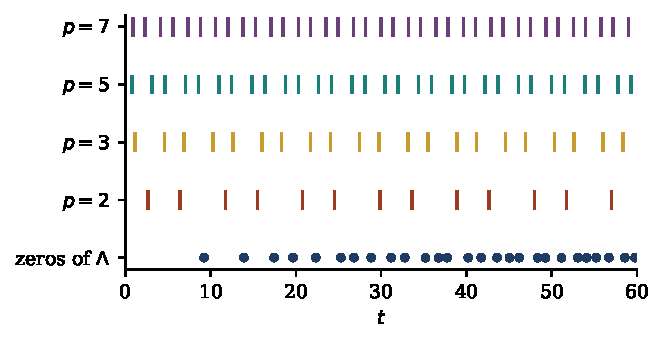
\includegraphics[width=\textwidth]{figs/thorin_combs.pdf}
\caption{Ordinates of the local zeros (local Thorin combs) of $\Delta$ at $p=2,3,5,7$, the progressions $(\pm\theta_p+2\pi\Z)/\log p$, against the ordinates $\gamma$ of the zeros of $\Lambda(s,\Delta)$ for $0<t<60$. Each comb is periodic with density $\log p/\pi$; the global zeros are not periodic.}\label{fig:10ccombs}
\end{figure}

\begin{remark}[Heuristic]
The combs of the primes $p\le P$ have total density $\sum_{p\le P}\log p/\pi\approx P/\pi$ by the prime number theorem, while the zeros of $L(s,\Delta)$ near height $t$ have density $\frac1\pi\log\frac{t}{2\pi}$. The two agree when $P\approx\log\frac{t}{2\pi}$: near height $t$, a truncated product of local GGCs over $p\lesssim\log t$ carries as many Thorin atoms per unit length as the global Thorin measure. This echoes the hybrid Euler Hadamard product $P_XZ_X$ of Gonek, Hughes and Keating \cite{ghk2007} (Section~\ref{sec:09bhybrid}), whose splitting conjecture is posed for $X=O((\log T)^{2-\varepsilon})$, a range that contains the matching scale $X\approx\log T$.
\end{remark}

The Euler product itself does not converge to a global GGC: the local means $(\log p)^2/(2-x_p)$ are not summable, and the global Thorin measure is not the sum of the local combs. The explicit formula, read through Proposition~\ref{prop:10cdictionary}, is the precise relation between them.

\section{Sato Tate random Euler products}\index{Thorin point process}

Model the angles $\theta_p$ as independent random variables with the Sato Tate law $\frac2\pi\sin^2\theta\,d\theta$ on $[0,\pi]$. By Theorem~\ref{thm:10clocal} every local reciprocal factor $f_{x_p}$, $x_p=2\cos\theta_p$, is the Laplace transform of a GGC almost surely (the only excluded value, $\theta_p=0$, has probability zero), and for every $P$ the truncated random Euler product
\[
\Phi_P(s)=\prod_{p\le P}\frac{2-x_p}{2\cosh(\sqrt s\log p)-x_p}
\]
is the Laplace transform of a GGC whose Thorin measure $\tau_P=\sum_{p\le P}\tau_{\theta_p,\log p}$ is random. We call $\tau_P$, or its preimage on the ordinate axis, a \emph{Thorin point process}.

\begin{proposition}[this book]\label{prop:10csatotate}
Let $\theta$ have the Sato Tate law and let $\epsilon=\pm1$ be an independent fair sign.
\begin{enumerate}
\item The configuration $\{\theta,-\theta\}$ on the circle $\R/2\pi\Z$ has intensity $\frac2\pi\sin^2\psi\,d\psi$, and $\epsilon\theta$ has density $\frac1\pi\sin^2\psi$ on $(-\pi,\pi]$.
\item The ordinates $(\pm\theta+2\pi\Z)/\log p$ of the comb of $p$ form a symmetric point process on $\R$ with intensity
\[
\frac{\log p}{\pi}\bigl(1-\cos(2t\log p)\bigr)\,dt .
\]
Consequently the Thorin point process of $\Phi_P$ has intensity $I_P(t)\,dt$ on the ordinate axis, $I_P(t)=\frac1\pi\sum_{p\le P}\log p\,(1-\cos(2t\log p))$.
\item $\E[(2-x_p)^{-1}]=1$, so the local law has expected mean $(\log p)^2$.
\end{enumerate}
\end{proposition}

\begin{proof}
(1) For a test function $\phi$ on the circle, $\E[\phi(\theta)+\phi(-\theta)]=\int_0^\pi(\phi(\psi)+\phi(-\psi))\frac2\pi\sin^2\psi\,d\psi=\int_{-\pi}^{\pi}\phi(\psi)\frac2\pi\sin^2\psi\,d\psi$, and half of this is $\E\phi(\epsilon\theta)$.

(2) Let $L=\log p$ and $\phi$ be compactly supported on $\R$. By (1) and unfolding the sum over $k$,
\begin{align*}
\E\sum_{k\in\Z}\Bigl[\phi\Bigl(\frac{\theta+2\pi k}{L}\Bigr)+\phi\Bigl(\frac{-\theta+2\pi k}{L}\Bigr)\Bigr]&=\sum_k\int_{-\pi}^{\pi}\phi\Bigl(\frac{\psi+2\pi k}{L}\Bigr)\frac2\pi\sin^2\psi\,d\psi\\
&=\int_{\R}\phi\Bigl(\frac uL\Bigr)\frac2\pi\sin^2u\,du,
\end{align*}
using periodicity of $\sin^2$. Substituting $u=Lt$ and $2\sin^2(Lt)=1-\cos(2Lt)$ gives the intensity. Intensities of independent superpositions add.

(3) With $x=2\cos\theta$, $2-x=4\sin^2(\theta/2)$ and $\sin^2\theta=4\sin^2(\theta/2)\cos^2(\theta/2)$, so $\E(2-x)^{-1}=\frac2\pi\int_0^\pi\cos^2(\theta/2)\,d\theta=1$. The mean of the local law is $L^2/(2-x)$ by Theorem~\ref{thm:10clocal}.
\end{proof}

Compare two other models. If $\theta_p$ is uniform on $[0,\pi]$ (the arcsine law for $x_p$), the comb of $p$ has flat intensity $\log p/\pi$. Under the law $\mu_{\mathrm{CM}}=\frac12\delta_0+\frac12\,$arcsine of Chapter~\ref{ch:04}, half the primes have $\theta_p=\pi/2$ and contribute the deterministic comb $(\frac12+\Z)\pi/\log p$, the other half the flat intensity, so the intensity is $\frac{\log p}{2\pi}+\frac12\sum_{k\in\Z}\delta_{(k+1/2)\pi/\log p}$. Only the Sato Tate model depletes the origin: $I_P(0)=0$ and $I_P(t)\le\frac{2t^2}{\pi}\sum_{p\le P}(\log p)^3$, a quadratic vanishing at $t=0$ (and at no other point once two primes are present). Part (3) shows the same effect in the mean: under the arcsine model $\E(2-x_p)^{-1}=\infty$, because angles near $0$ put Thorin atoms near the origin, while under Sato Tate the depletion makes the expected mean finite.

We read this cautiously. Of the one level densities of Section~\ref{sec:ch6ks}, $W(\USp)$ vanishes quadratically at the central point, and so does $W(\mathrm{SO(odd)})$ once the forced central zero is removed, while $W(\mathrm{SO(even)})$ does not \cite{ils2000,katzsarnak1999}. The Sato Tate depletion near $t=0$ is a local mechanism with the sign and the order of vanishing of the symplectic case, built prime by prime from the factor $\sin^2$ in the Haar measure of $\SU(2)=\USp(2)$. At the scale $t\asymp1/\log P$ the prime number theorem gives $I_P(t)=\frac1\pi\bigl(\vartheta(P)-\Re\frac{P^{1+2it}}{1+2it}\bigr)+o(P)$, with $\vartheta$ Chebyshev's function, so the depletion has width of order $1/\log P$. We do not claim that the global one level density is a consequence of this local picture; the heuristic of the previous section suggests matching $\log P$ with $\log\log t$, and making any such statement precise is open.

\section[Function fields and graphs: unconditional global Thorin]{Function fields and graphs:\\ unconditional global Thorin}\index{function field}

Let $C$ be a smooth projective geometrically connected curve of genus $g\ge1$ over $\mathbb F_q$. Its zeta function is
\[
Z(C,u)=\frac{P(u)}{(1-u)(1-qu)},\qquad P(u)=\prod_{j=1}^{2g}(1-\alpha_ju)\in\Z[u],\qquad u=q^{-s},
\]
and the functional equation makes the multiset $\{\alpha_j\}$ stable under $\alpha\mapsto q/\alpha$. Pair the roots accordingly, and for each pair put $c_j=(\alpha_j+q/\alpha_j)/\sqrt q$, $1\le j\le g$. With $z=s-\frac12$ and $u=q^{-1/2-z}$, each pair gives $(1-\alpha_ju)(1-(q/\alpha_j)u)=q^{-z}\bigl(2\cosh(z\log q)-c_j\bigr)$, so
\[
\Xi_C(z):=q^{gz}P(q^{-1/2-z})=\prod_{j=1}^g\bigl(2\cosh(z\log q)-c_j\bigr),
\]
an even entire function, real on the real axis. The Riemann hypothesis for $C$ is $|\alpha_j|=\sqrt q$ for all $j$, equivalently $c_j=2\cos\theta_j\in[-2,2]$ with $\alpha_j=\sqrt q\,e^{i\theta_j}$. It was proved by Weil \cite{weil1948}, and in all dimensions by Deligne \cite{deligne1974}. Put $F_C(s)=\Xi_C(\sqrt s)/\Xi_C(0)$.

\begin{theorem}[this book]\label{thm:10ccurve}
Assume $P(q^{-1/2})\ne0$, that is, no $\alpha_j$ equals $\sqrt q$. Then $s\mapsto1/F_C(s)$ is the Laplace transform of a GGC if and only if the Riemann hypothesis holds for $C$. In that case the Thorin measure is the finite superposition of periodic combs
\[
\tau_C=\sum_{j=1}^g\sum_{k\in\Z}\delta_{((\theta_j+2\pi k)/\log q)^2},
\]
and the law is $\sum_j\sum_kE_{j,k}\,(\log q)^2/(\theta_j+2\pi k)^2$, with mean $(\log q)^2\sum_j(2-c_j)^{-1}$. By Weil's theorem all of this holds unconditionally.
\end{theorem}

\begin{proof}
If the Riemann hypothesis holds then every $c_j\in[-2,2)$, the value $2$ being excluded by $P(q^{-1/2})\ne0$, and $1/F_C=\prod_jf_{c_j}$ with $L=\log q$. Each factor is a GGC transform with Thorin measure $\tau_{\theta_j,\log q}$ by Theorem~\ref{thm:10clocal}, and GGCs are closed under convolution, Thorin measures adding. Conversely, suppose $1/F_C$ agrees on $(0,\infty)$ with the Laplace transform $\varphi$ of a GGC. By Lemma~\ref{lem:ch10nonvanish}, $\varphi F_C$ is holomorphic on $\C\setminus(-\infty,0]$, and it equals $1$ on $(0,\infty)$, hence everywhere; so the entire function $s\mapsto\Xi_C(\sqrt s)$ has no zeros off $(-\infty,0]$, and since $\Xi_C(0)\ne0$ every zero $z$ of $\Xi_C$ is purely imaginary. A zero of $2\cosh(z\log q)-c_j$ with $z=iy$ satisfies $\cos(y\log q)=c_j/2$, which forces $c_j\in[-2,2]$. Hence every $c_j$ is real in $[-2,2]$ and $|\alpha_j|=\sqrt q$.
\end{proof}

\begin{example}
For $C:y^2=x^5-x+1$ over $\mathbb F_{101}$ (genus $2$) the characteristic polynomial of Frobenius, computed for this book, is $T^4+8T^3-16T^2+808T+10201$, so $\#C(\mathbb F_{101})=110$. All roots have absolute value $\sqrt{101}$, with angles $\theta_1=0.973934$, $\theta_2=2.858029$, so $c_1=1.124099$, $c_2=-1.920129$ and $\Xi_C(0)=P(101^{-1/2})=3.433644$. The smallest Thorin atoms are $0.044534$, $0.383502$, $0.550801$, $1.323428$, and the GGC has mean $29.7504$. The product identity of Lemma~\ref{lem:10cproduct} at these angles, truncated at $|k|\le20000$, was checked to relative error $1.3\times10^{-5}$.
\end{example}

The same holds for regular graphs. Let $G$ be a finite connected $(q+1)$ regular graph with adjacency eigenvalues $\lambda_j$. By the Ihara Bass formula of Chapter~\ref{ch:08}, each eigenvalue contributes $1-\lambda_ju+qu^2=q^{-z}(2\cosh(z\log q)-\lambda_j/\sqrt q)$ at $u=q^{-1/2-z}$. The trivial eigenvalue $q+1$ gives $x=\sqrt q+1/\sqrt q>2$, which in Theorem~\ref{thm:10clocal} is a positive real pole: it plays the role of the pole of $\zeta$ at $s=1$, and the Thorin criterion rejects it, as the global criterion must reject the pole. Put
\[
\Xi_G(z)=\prod_{|\lambda_j|<q+1}\Bigl(2\cosh(z\log q)-\frac{\lambda_j}{\sqrt q}\Bigr),\qquad F_G(s)=\frac{\Xi_G(\sqrt s)}{\Xi_G(0)} .
\]

\begin{theorem}[this book]\label{thm:10cihara}\index{Ramanujan graph}
Suppose no eigenvalue of $G$ equals $2\sqrt q$. Then $G$ is Ramanujan if and only if $1/F_G$ is the Laplace transform of a GGC, and then its Thorin measure is $\sum_j\sum_{k\in\Z}\delta_{((\theta_j+2\pi k)/\log q)^2}$ over the nontrivial eigenvalues $\lambda_j=2\sqrt q\cos\theta_j$. For the supersingular $\ell$ isogeny graphs $G_N(\ell)$ of Chapter~\ref{ch:08}, with $N\equiv1\bmod12$ and $\ell\ne N$ primes, both hold unconditionally.
\end{theorem}

\begin{proof}
The first statement is the proof of Theorem~\ref{thm:10ccurve} with $c_j=\lambda_j/\sqrt q$. For $G_N(\ell)$, Theorem~\ref{thm:08brandt} identifies the nontrivial spectrum with the eigenvalues of $T_\ell$ on $S_2(\Gamma_0(N))$, which satisfy $|\lambda|\le2\sqrt\ell$. The eigenvalue $2\sqrt\ell$ does not occur: $\lambda=\pm2\sqrt\ell$ would mean equal Satake parameters, excluded in weight two by Coleman and Edixhoven \cite{colemanedixhoven1998}.
\end{proof}

The shape of the Thorin measures separates function fields from $\Q$. Over a function field the global Thorin measure is a finite superposition of $g$ periodic combs with common period $2\pi/\log q$ on the ordinate axis, because $\Xi_C$ is a polynomial in $\cosh(z\log q)$. Over $\Q$ the ordinates that carry the global Thorin measure of Chapter~\ref{ch:10b} are aperiodic, with density growing like $\log t$, and the explicit formula, read through Proposition~\ref{prop:10cdictionary}, shows them as the interference pattern of infinitely many local combs, each damped by its half shift, whose base frequencies $\log p$ are linearly independent over $\Q$ by unique factorisation. Ramanujan is local Thorin in both worlds; global Thorin is known only where there is one comb period.

\section{Hecke walks and Thorin measures of passage times}\index{Keilson's theorem}\index{passage time}

In this section the Thorin measures are spectra. Let $Y$ be a birth death process on $\{0,1,\dots,n\}$ with birth rates $b_k>0$ ($0\le k<n$) and death rates $d_k>0$ ($1\le k\le n$), reflecting at $0$, started at $0$, and let $T$ be its first passage time to $n$. Let $Q_n$ be the generator restricted to $\{0,\dots,n-1\}$ (killed at $n$).

\begin{theorem}[Keilson \cite{keilson1971}]\label{thm:10ckeilson}
The eigenvalues $\lambda_1<\dots<\lambda_n$ of $-Q_n$ are real, simple and positive, and $T$ has the law of $\sum_{j=1}^nE_j/\lambda_j$. In particular $T$ is a GGC with Thorin measure $\sum_j\delta_{\lambda_j}$, and $\E e^{-sT}=\det(-Q_n)/\det(sI-Q_n)$.
\end{theorem}

\begin{proof}
For $s>0$ let $u_k=\E_ke^{-sT}$, $0\le k<n$. First step analysis gives $(sI-Q_n)u=b_{n-1}e_{n-1}$. By Cramer's rule $u_0$ is $b_{n-1}$ times the $(n-1,0)$ cofactor of $sI-Q_n$, divided by $\det(sI-Q_n)$. Deleting row $n-1$ and column $0$ of the tridiagonal matrix $sI-Q_n$ leaves a triangular matrix with diagonal $-b_0,\dots,-b_{n-2}$, so the cofactor equals $b_0\cdots b_{n-2}$, independent of $s$. Hence $u_0=b_0\cdots b_{n-1}/\det(sI-Q_n)$, and letting $s\to0$, where $u_0\to\Prob_0(T<\infty)=1$, gives $\det(-Q_n)=b_0\cdots b_{n-1}\ne0$. The matrix $-Q_n$ is similar, by the diagonal matrix of square roots of the reversible weights, to a symmetric Jacobi matrix with nonzero off diagonal entries $-\sqrt{b_kd_{k+1}}$; so its eigenvalues are real and simple. Each row of $-Q_n$ has diagonal entry at least the sum of the moduli of its off diagonal entries, so by Gershgorin's theorem the eigenvalues are nonnegative, and since $\det(-Q_n)\ne0$ they are positive. Therefore $\E e^{-sT}=\prod_j\lambda_j/(s+\lambda_j)$, the Laplace transform of $\sum_jE_j/\lambda_j$.
\end{proof}

Kent proved the analogue for one dimensional diffusions, with infinitely many rates \cite{kent1980}, and Fill gave a probabilistic proof by a stochastic construction of the exponential stages \cite{fill2009}. An exercise of Chapter~\ref{ch:10} uses the hitting time of a Bessel process in the same way.

Let $\T_q$ be the $(q+1)$ regular tree, the Bruhat Tits tree of $\PGL_2(\Q_q)$ for $q$ prime, and run continuous time simple random walk on it, jumping at rate $1$ to a uniformly chosen neighbour; this is the Hecke walk with generator $(q+1)^{-1}A-I$, where $A=T_q$ is the adjacency operator of Chapter~\ref{ch:07}. Let $T_n$ be the first time at distance $n$ from the start. The distance is a birth death process with $b_0=1$, and $b_k=\frac{q}{q+1}$, $d_k=\frac1{q+1}$ for $k\ge1$. Symmetrising,
\[
-Q_n\sim J_n=I-S_n,\qquad S_n=\begin{pmatrix}0&a&&&\\a&0&c&&\\&c&0&\ddots&\\&&\ddots&\ddots&c\\&&&c&0\end{pmatrix},
\]
with $a=1/\sqrt{q+1}$ and $c=\sqrt q/(q+1)=\rho/2$, where $\rho=2\sqrt q/(q+1)$ is the Kesten spectral radius.

\begin{theorem}[Passage times on the tree, this book]\label{thm:10ctree}\index{Kesten band}
Let $q\ge2$, $\rho=2\sqrt q/(q+1)$, and let $\lambda_1<\dots<\lambda_n$ be the Thorin atoms of $T_n$.
\begin{enumerate}
\item $\lambda_j=1-\frac{\sqrt q}{q+1}x_j$, where $x_1>\dots>x_n$ are the zeros of the polynomial $U_n(x/2)-q^{-1}U_{n-2}(x/2)$ that expresses $B_n=q^{-n/2}A_n$ in terms of $X=q^{-1/2}A$ (Theorem~\ref{thm:07tree}). All $x_j$ lie in $(-2,2)$, so all rates lie in the Kesten band $(1-\rho,1+\rho)$.
\item $\frac1n\sum_j\delta_{\lambda_j}$ converges weakly to the law of $1-\rho\cos(\pi U)$, $U$ uniform on $(0,1)$: the arcsine law on the Kesten band.
\item $\E T_n=\frac{n(q+1)}{q-1}-\frac{2q(1-q^{-n})}{(q-1)^2}$, and $\E T_n/n\to\frac{q+1}{q-1}=\frac1{\sqrt{1-\rho^2}}=\int_0^1\frac{du}{1-\rho\cos\pi u}$. The escape speed of the walk is $\frac{q-1}{q+1}=\sqrt{1-\rho^2}$.
\item $\mathrm{Var}\,T_n/n\to\bigl(\frac{q+1}{q-1}\bigr)^3=(1-\rho^2)^{-3/2}$, and $(T_n-\E T_n)/\sqrt{\mathrm{Var}\,T_n}$ converges in law to a standard normal.
\end{enumerate}
\end{theorem}

\begin{proof}
(1) Let $D_k$ be the characteristic polynomial of the leading $k\times k$ block of $c^{-1}S_n$, whose first off diagonal entry is $a/c=\sqrt{1+1/q}$ and the others $1$. Expanding along the last row, $D_1=x$, $D_2=x^2-1-q^{-1}$ and $D_{k+1}=xD_k-D_{k-1}$ for $k\ge2$. The polynomials $U_k(x/2)-q^{-1}U_{k-2}(x/2)$, with $U_{-1}=0$, satisfy the same recursion for $k\ge2$ and agree with $D_1$, $D_2$ and $D_3=x^3-(2+q^{-1})x$ at $k=1,2,3$, so they equal $D_k$; by Theorem~\ref{thm:07tree}(1) this is the polynomial of $B_k$. The eigenvalues of $S_n$ are $cx_j$, so $\lambda_j=1-cx_j$. To locate the zeros put $x=2\cos\phi$, $0<\phi<\pi$; then $D_n=g(\phi)/\sin\phi$ with
\[
g(\phi)=\sin((n+1)\phi)-q^{-1}\sin((n-1)\phi).
\]
At $\phi_k^*=(k+\frac12)\pi/(n+1)$, $0\le k\le n$, $|\sin((n+1)\phi)|=1>q^{-1}$, so $g(\phi_k^*)$ has the sign $(-1)^k$. Hence $g$ has a zero $\phi_j$ in each interval $(\phi_{j-1}^*,\phi_j^*)$, $1\le j\le n$. These are $n$ distinct zeros in $(0,\pi)$, and $D_n$ has degree $n$, so they are all the zeros and $x_j=2\cos\phi_j\in(-2,2)$. Since $c\cdot2=\rho$, $\lambda_j=1-\rho\cos\phi_j\in(1-\rho,1+\rho)$.

Conceptually, $S_n$ is a compression of the radial part of $P=(q+1)^{-1}A$, whose spectrum lies in $[-\rho,\rho]$ by Kesten's theorem~\cite{kesten1959}, so the rates cannot leave the closed Kesten band.

(2) The bracketing $\phi_j\in(\phi_{j-1}^*,\phi_j^*)$ gives $|\phi_j-j\pi/(n+1)|<\pi/(2(n+1))$, so for continuous $\psi$ on $[1-\rho,1+\rho]$, $\frac1n\sum_j\psi(1-\rho\cos\phi_j)$ is a Riemann sum converging to $\int_0^1\psi(1-\rho\cos\pi u)\,du$. It also follows from Szeg\H{o}'s theorem for Toeplitz matrices \cite{grenandersz}, since $S_n$ differs from the tridiagonal Toeplitz matrix with symbol $\rho\cos\phi$ by a perturbation of rank two, and by interlacing such a perturbation moves the empirical spectral measure by at most $2/n$ in Kolmogorov distance.

(3) Let $m_k$ be the expected time to go from distance $k$ to $k+1$. Then $m_0=1$, and for $k\ge1$ the walk waits a mean unit time and then moves down with probability $\frac1{q+1}$, after which it needs $m_{k-1}+m_k$ more on average: $m_k=1+\frac{1}{q+1}(m_{k-1}+m_k)$, that is $m_k=\frac{q+1}{q}+\frac{m_{k-1}}{q}$. With $m^*=\frac{q+1}{q-1}$ this is $m_k-m^*=(m_{k-1}-m^*)/q$, so $m_k=m^*-\frac{2}{q-1}q^{-k}$, and summing $k=0,\dots,n-1$ gives the formula. The limit of $\E T_n/n=\frac1n\sum_j\lambda_j^{-1}$ also follows from (2), since $1/\lambda$ is continuous on the band, together with $\int_0^\pi\frac{d\phi}{\pi(1-\rho\cos\phi)}=(1-\rho^2)^{-1/2}$ and $1-\rho^2=\bigl(\frac{q-1}{q+1}\bigr)^2$. For the speed, away from $0$ the distance jumps at rate $1$, up with probability $\frac q{q+1}$ and down with probability $\frac1{q+1}$, and it visits $0$ only finitely often, so by the law of large numbers the distance at time $t$ divided by $t$ tends almost surely to $\frac{q-1}{q+1}=1/m^*$.

(4) $\mathrm{Var}\,T_n=\sum_j\lambda_j^{-2}$, and (2) with $\int_0^\pi\frac{d\phi}{\pi(1-\rho\cos\phi)^2}=(1-\rho^2)^{-3/2}$ gives the limit. The summands $E_j/\lambda_j$ are independent with $\E|E_j-1|^3\lambda_j^{-3}\le C(1-\rho)^{-3}$, so the Lyapunov ratio is $O(n(1-\rho)^{-3}/n^{3/2})\to0$.
\end{proof}

Thus the Thorin rates of the passage time are $1-\frac{\sqrt q}{q+1}x$ with $x$ in the tempered spectrum $[-2,2]$: the statement \emph{Thorin support in the Kesten band} is the random walk form of the Ramanujan bound. Kesten's spectral radius determines the escape speed through the arcsine average of the reciprocal rates; in Chapter~\ref{ch:07} the same number is the drift $\frac{q-1}{q+1}$ of the distance chain, whose gambler's ruin gives the return probability $1/q$.

The theorem also gives exact large deviations. Since all rates exceed $1-\rho$, $\E e^{\theta T_n}=\prod_j(1-\theta/\lambda_j)^{-1}$ is finite for $\theta\le1-\rho$, and we can compute the limit through the Thorin measure.

\begin{theorem}[Large deviations of passage times, this book]\label{thm:10cldp}
For $\theta\le1-\rho$,
\[
\lim_{n\to\infty}\frac1n\log\E e^{\theta T_n}=\Lambda(\theta)=-\log\frac{(q+1)\bigl(1-\theta+\sqrt{(1-\theta)^2-\rho^2}\bigr)}{2q},
\]
and the limit is $+\infty$ for $\theta>1-\rho$. In particular $\Lambda(1-\rho)=\frac12\log q$. The function $\Lambda$ is steep, $\Lambda'(\theta)=((1-\theta)^2-\rho^2)^{-1/2}\to\infty$ as $\theta\uparrow1-\rho$, so $T_n/n$ satisfies a large deviation principle with good rate function
\[
\Lambda^*(y)=y-\sqrt{1+\rho^2y^2}+\log\frac{(q+1)\bigl(1+\sqrt{1+\rho^2y^2}\bigr)}{2qy},\qquad y>0,
\]
which vanishes only at $y=\frac{q+1}{q-1}$.
\end{theorem}

\begin{proof}
For $\theta<1-\rho$, $\frac1n\log\E e^{\theta T_n}=\frac1n\sum_j\bigl[\log\lambda_j-\log(\lambda_j-\theta)\bigr]$, and the integrand is continuous on the band, so by Theorem~\ref{thm:10ctree}(2) the limit is $\int_0^\pi[\log(1-\rho\cos\phi)-\log(1-\theta-\rho\cos\phi)]\frac{d\phi}{\pi}$. The classical integral $\int_0^\pi\log(a-b\cos\phi)\frac{d\phi}\pi=\log\frac{a+\sqrt{a^2-b^2}}{2}$ for $a\ge|b|$, together with $1+\sqrt{1-\rho^2}=\frac{2q}{q+1}$, gives $\Lambda$. At $\theta=1-\rho$ the second term becomes $\log(\rho(1-\cos\phi))$, which is singular at $\phi=0$, but it is increasing in $\phi$ and integrable, and the bracketing of the $\phi_j$ in intervals of length $\pi/(n+1)$ shows that its Riemann sums converge to the integral (the term $j=1$ is $O(n^{-1}\log n)$). The value is $-\log\frac{(q+1)\rho}{2q}=\frac12\log q$. For $\theta>1-\rho$, $\lambda_1\to1-\rho$ by (2), so $\E e^{\theta T_n}=\infty$ for large $n$. Differentiating, $\Lambda'(\theta)=((1-\theta)^2-\rho^2)^{-1/2}$, which tends to infinity at the edge, so $\Lambda$ is essentially smooth with $0$ in the interior of its domain and the G\"artner Ellis theorem \cite{dembozeitouni1998} applies. Since $\Lambda'$ maps $(-\infty,1-\rho)$ onto $(0,\infty)$, the supremum in $\Lambda^*(y)=\sup_\theta[\theta y-\Lambda(\theta)]$ is attained at $1-\theta=\sqrt{\rho^2+y^{-2}}$, and substituting gives the formula. At $y=(1-\rho^2)^{-1/2}$ one finds $\sqrt{1+\rho^2y^2}=y$ and $\Lambda^*(y)=0$.
\end{proof}

The value $\Lambda(1-\rho)=\frac12\log q$ is half the logarithm of the branching number: at the edge of the Kesten band the exponential moment grows like $q^{n/2}$, and indeed the closed form $\E e^{(1-\rho)T_n}=\frac{q+1}{q}\,q^{n/2}\big/\bigl(n+1-\frac{n-1}{q}\bigr)$, which follows from Theorem~\ref{thm:10ckeilson} and the values of $D_n$ at $x=2$ and $x=1/c$, shows the polynomial correction. For $q=2$ and $n=6400$ it gives $\frac1n\log\E e^{(1-\rho)T_n}=0.345376$, the value computed from the rates, against the limit $\frac12\log2=0.346574$.

The numbers, computed for this book from the Jacobi matrices $J_n$ for $q=2,3,5$ and $n=100,400,1600,6400$, confirm every statement. All rates lie in $(1-\rho,1+\rho)$; at $n=6400$ the smallest rates are $0.05719$, $0.13397$, $0.25464$ against gaps $1-\rho=0.057191$, $0.133975$, $0.254644$. The ratios $\E T_n/n$ are $2.99938$, $1.99977$, $1.49990$ against $3$, $2$, $1.5$, and $\mathrm{Var}\,T_n/n=26.9856$, $7.9975$, $3.3744$ against $27$, $8$, $3.375$. The trace $\mathrm{tr}\,J_n^{-1}=19196$ for $q=2$, $n=6400$ equals the formula of (3). The Kolmogorov distance of the rescaled rates to the arcsine law is $8\times10^{-5}$ at $n=6400$. For $q=2$ and $n=6400$, $\frac1n\log\E e^{\theta T_n}$ is $-0.693095$ at $\theta=-0.5$ against $\Lambda=-0.693147$, and $0.100872$ at $\theta=(1-\rho)/2=0.0286$ against $0.100899$. A simulation of $20000$ walks with $q=2$, $n=100$ gave mean $296.07$, against $296.24$ for an equal sample from $\sum E_j/\lambda_j$ and the exact value $296$; the Kolmogorov Smirnov test comparing the two samples has $p=0.57$ (Figure~\ref{fig:10ctree}).

\begin{figure}[t]\centering
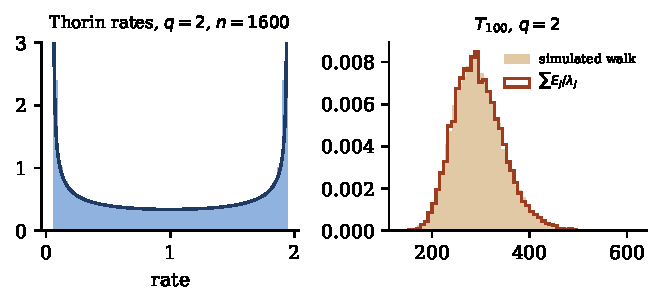
\includegraphics[width=\textwidth]{figs/thorin_tree.pdf}
\caption{Left: the Thorin atoms of $T_{1600}$ for $q=2$ against the arcsine density on the Kesten band $(1-\rho,1+\rho)$. Right: simulated passage times $T_{100}$ ($q=2$, $20000$ walks) against the GGC $\sum_jE_j/\lambda_j$ of Theorem~\ref{thm:10ckeilson}.}\label{fig:10ctree}
\end{figure}

\section{Exponential hitting times on Ramanujan graphs}\index{hitting time}\index{Aldous Brown inequality}

On a finite graph a passage time is no longer a pure GGC, but the spectral structure survives. Let $G$ be a connected $(q+1)$ regular graph with vertex set $V$ of size $h$ that is not bipartite. Loops and multiple edges are allowed, but the adjacency matrix $A$ is symmetric, as for the Brandt matrices of Chapter~\ref{ch:08} when $N\equiv1\bmod12$. Let $P=(q+1)^{-1}A$, with eigenvalues $1=p_1>p_2\ge\dots\ge p_h>-1$ (written $\mu_j$ in Appendix~\ref{app:A}; below, $\mu_j$ is a rate), and run the continuous time walk with generator $P-I$. Fix a target $v$ and let $\tau_v$ be its hitting time. Let $P_v$ be the principal submatrix of $P$ on $V\setminus\{v\}$, with eigenvalues $r_1\ge r_2\ge\dots\ge r_{h-1}$ and orthonormal eigenvectors $\psi_j$, and put $\mu_j=1-r_j$, the \emph{Dirichlet rates}.

\begin{proposition}\label{prop:10cmixture}
Started from the uniform law $\pi$,
\[
\Prob_\pi(\tau_v>t)=\sum_{j=1}^{h-1}w_je^{-\mu_jt},\qquad w_j=\frac1h\langle\vec 1,\psi_j\rangle^2\ge0,\qquad \sum_jw_j=\frac{h-1}{h},
\]
a completely monotone mixture of exponentials, and $\E_\pi\tau_v=\sum_jw_j/\mu_j\ge(h-1)^2/h$.
\end{proposition}

\begin{proof}
Killing at $v$, $\Prob_x(\tau_v>t)=(e^{-t(I-P_v)}\vec 1)(x)$ for $x\ne v$, and averaging over $x$ with weight $1/h$ gives the mixture by the spectral theorem for the symmetric matrix $P_v$. Connectedness makes $I-P_v$ positive definite. For the mean, $\E_\pi\tau_v=\frac1h\langle\vec 1,(I-P_v)^{-1}\vec 1\rangle$, and the Cauchy Schwarz inequality for the positive definite form gives $\langle\vec 1,M^{-1}\vec 1\rangle\langle\vec 1,M\vec 1\rangle\ge\langle\vec 1,\vec 1\rangle^2$ with $M=I-P_v$. Here $\langle\vec 1,\vec 1\rangle=h-1$, and since $P$ is symmetric and stochastic, $\langle\vec 1,M\vec 1\rangle=(h-1)-\sum_{x,y\ne v}P(x,y)=\sum_{x\ne v}P(x,v)=1-P(v,v)\le1$.
\end{proof}

The mixture form is classical (Keilson); see Aldous and Fill \cite{aldousfill}. By Cauchy interlacing the Dirichlet rates interlace the graph rates $1-p_j$, and these are what the Ramanujan bound controls.

\begin{theorem}[this book]\label{thm:10cexpo}
If $G$ is Ramanujan then $\mu_2,\dots,\mu_{h-1}\in[1-\rho,1+\rho]$, $\rho=2\sqrt q/(q+1)$: only the slowest Dirichlet rate $\mu_1\le1-p_2$ can leave the Kesten band. Moreover, for every target $v$,
\begin{align*}
\sup_{t\ge0}\bigl|\Prob_\pi(\tau_v>t)-e^{-t/\E_\pi\tau_v}\bigr|&\le\frac{\tau_2}{\E_\pi\tau_v}\le\frac{(q+1)\,h}{(\sqrt q-1)^2(h-1)^2}\\
&\le\frac{2(q+1)}{(\sqrt q-1)^2(h-1)},
\end{align*}
where $\tau_2=1/(1-p_2)$ is the relaxation time.
\end{theorem}

\begin{proof}
By Cauchy interlacing for the principal submatrix $P_v$ of the symmetric matrix $P$, $p_j\ge r_j\ge p_{j+1}$ for $1\le j\le h-1$. The Ramanujan property says $p_2,\dots,p_h\in[-\rho,\rho]$. For $j\ge2$, $r_j\le p_j\le p_2\le\rho$, and for all $j\le h-1$, $r_j\ge p_{j+1}\ge p_h\ge-\rho$. Hence $\mu_j=1-r_j\in[1-\rho,1+\rho]$ for $2\le j\le h-1$, and $\mu_1=1-r_1\le1-p_2$. The first inequality in the display is the Aldous Brown inequality for reversible chains started from stationarity \cite{aldousbrown1992,aldousfill}. Ramanujan gives $1-p_2\ge1-\rho=(\sqrt q-1)^2/(q+1)$, so $\tau_2\le(q+1)/(\sqrt q-1)^2$, and Proposition~\ref{prop:10cmixture} gives $\E_\pi\tau_v\ge(h-1)^2/h\ge(h-1)/2$.
\end{proof}

\begin{corollary}[Unconditional exponential law, this book]\label{cor:10cisogeny}
Let $N>13$ be a prime with $N\equiv1\bmod12$, so that $h=(N-1)/12\ge2$, and let $\ell\ne N$ be prime. For simple random walk in continuous time on the supersingular $\ell$ isogeny graph $G_N(\ell)$, every vertex $v$ satisfies
\[
\sup_{t\ge0}\bigl|\Prob_\pi(\tau_v>t)-e^{-t/\E_\pi\tau_v}\bigr|\le\frac{2(\ell+1)}{(\sqrt\ell-1)^2(h-1)},
\]
and all Dirichlet rates but the slowest lie in the Kesten band $[1-\rho_\ell,1+\rho_\ell]$, $\rho_\ell=2\sqrt\ell/(\ell+1)$.
\end{corollary}

\begin{proof}
By Theorem~\ref{thm:08brandt} every nontrivial eigenvalue satisfies $|\lambda|\le2\sqrt\ell<\ell+1$. Hence $\ell+1$ is a simple eigenvalue and $-(\ell+1)$ is not an eigenvalue, so $G_N(\ell)$ is connected, not bipartite and Ramanujan, and Theorem~\ref{thm:10cexpo} applies.
\end{proof}

Theorem~\ref{thm:08kemeny} supplies the scale. In continuous time at rate $1$ the expected hitting times are the discrete ones, so $\sum_v\pi(v)\E_\pi\tau_v$ is Kemeny's constant $K_N$, and $K_N/h\to\ell/(\ell-1)$. So on large isogeny graphs the time to find a given curve from a random start is, uniformly in time and up to $O(1/h)$, exponential, with a mean that averages over targets to about $\frac{\ell}{\ell-1}h$, that is about $2h$ for $\ell=2$.

The data, computed for this book on the supersingular $2$ isogeny graphs at $N=1009$, $2017$, $4129$, $7993$ ($h=84$, $168$, $344$, $666$) with six random targets each, are as follows. The largest observed $\sup_t|\Prob_\pi(\tau_v>t)-e^{-t/\E_\pi\tau_v}|$ is $0.0248$, $0.0144$, $0.0075$, $0.0039$; the Aldous Brown bound $\tau_2/\E_\pi\tau_v$ is $0.081$, $0.045$, $0.023$, $0.0127$; the Ramanujan bound of Corollary~\ref{cor:10cisogeny} is $0.421$, $0.209$, $0.102$, $0.0526$. The spectral gaps $1-p_2$ are $0.0845$, $0.0708$, $0.0642$, $0.0601$, above the Ramanujan lower bound $1-\rho_2=0.0572$; the smallest second Dirichlet rates are $\mu_2=0.0862$, $0.0710$, $0.0642$, $0.0601\ge0.0572$, and the largest Dirichlet rate is at most $1.9406\le1+\rho_2=1.9428$. All three quantities decay like $1/h$ (Figure~\ref{fig:10cisogeny}); the observed error is about a third of the Aldous Brown bound.

\begin{figure}[t]\centering
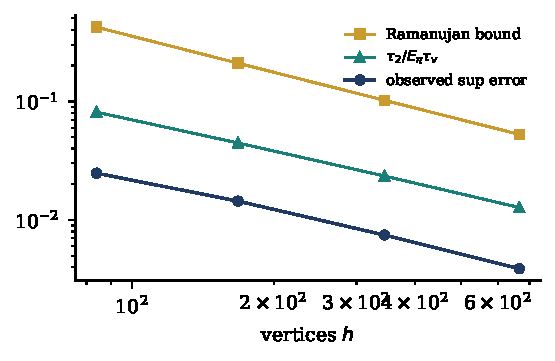
\includegraphics[width=0.8\textwidth]{figs/thorin_isogeny.pdf}
\caption{Supersingular $2$ isogeny graphs for $N=1009$, $2017$, $4129$, $7993$ ($h=84$ to $666$ vertices), six random targets $v$ each, logarithmic axes: the largest observed sup distance between $\Prob_\pi(\tau_v>t)$ and the exponential law with the same mean, against the largest Aldous Brown bound $\tau_2/\E_\pi\tau_v$ and the unconditional Ramanujan bound of Corollary~\ref{cor:10cisogeny}.}\label{fig:10cisogeny}
\end{figure}

\section{Extreme values and exponent measures}\index{max infinitely divisible}

Chapter~\ref{ch:11} represents $\prod_n(1-e^{-2\pi ny})$ as the distribution function of $M=\max_nE_n/(2\pi n)$. Here we identify the structure of $M$ in the language of this chapter: just as a GGC has a completely monotone L\'evy density, $M$ has a completely monotone exponent function. Write $\sigma_{-1}(m)=\sum_{d\mid m}d^{-1}$ and $P(y)=\Prob(M\le y)$ as in Chapter~\ref{ch:11}.

\begin{proposition}[this book]\label{prop:10cmaxid}
\begin{enumerate}
\item Let $G=-\log P$. Then for $y>0$
\[
G(y)=\sum_{m\ge1}\sigma_{-1}(m)\,e^{-2\pi my}.
\]
Hence $G$ is completely monotone, $G(y)=\int e^{-yu}\nu(du)$ with
\[
\nu=\sum_{m\ge1}\sigma_{-1}(m)\,\delta_{2\pi m},
\]
and $M$ is max infinitely divisible.
\item For each $n$, $E_n/(2\pi n)$ has the law of $\max_{k\ge1}\max_{i\le N_k}E_{k,i}/(2\pi nk)$, with $N_k$ Poisson of mean $1/k$, all variables independent. Consequently $M$ has the law of $\max_{m\ge1}\max_{i\le N'_m}E'_{m,i}/(2\pi m)$ with independent $N'_m$ Poisson of mean $\sigma_{-1}(m)$.
\item For $\Re s>1$, $\int_0^\infty G(y)y^{s-1}dy=\Gamma(s)(2\pi)^{-s}\zeta(s)\zeta(s+1)$. The right side continues meromorphically to $\C$ with poles only at $s=0,\pm1$, and is invariant under $s\mapsto-s$.
\item For $f=\prod_m\eta(m\tau)^{r_m}$ with $r_m\ge0$, $\sum_mmr_m=24$, and $M_f$ as in Theorem~\ref{thm:ch11general}, $-\log\Prob(M_f\le y)=\sum_mr_mG(my)$ is completely monotone with exponent measure $\sum_n\big(\sum_{m\mid n}r_m\sigma_{-1}(n/m)\big)\delta_{2\pi n}$, and its Mellin transform is $\Gamma(s)(2\pi)^{-s}\zeta(s)\zeta(s+1)\sum_mr_mm^{-s}$.
\end{enumerate}
\end{proposition}

\begin{proof}
(1) $-\log(1-e^{-2\pi ny})=\sum_{k\ge1}e^{-2\pi nky}/k$; summing over $n$ and collecting $m=nk$ gives $\sum_me^{-2\pi my}\sum_{k\mid m}k^{-1}$, and $\sum_{k\mid m}k^{-1}=\sigma_{-1}(m)$. A positive combination of decreasing exponentials is completely monotone. For every $t>0$, $P^t=\exp(-tG)$ is the distribution function of the maximum of a Poisson process with intensity $t\sum_m\sigma_{-1}(m)\,\mathrm{Law}(E/(2\pi m))$ by the computation in (2), so $M$ is max infinitely divisible \cite{resnick1987}.

(2) If $N$ is Poisson of mean $\lambda$, independent of the $Z_i$, independent copies of $Z$, then $\Prob(\max_{i\le N}Z_i\le y)=\E\Prob(Z\le y)^N=\exp(-\lambda\Prob(Z>y))$, with an empty maximum read as $0$. For $Z=E/(2\pi nk)$ and $\lambda=1/k$ this is $\exp(-e^{-2\pi nky}/k)$, and the product over $k$ is $\exp(\log(1-e^{-2\pi ny}))=1-e^{-2\pi ny}=\Prob(E_n/(2\pi n)\le y)$, by the identity $1-e^{-x}=\exp(-\sum_ke^{-kx}/k)$ for $x>0$. The maximum is almost surely over a nonempty set, since $\sum_k1/k=\infty$. Taking independent copies for all $n$ and merging the Poisson families with the same $m=nk$ (superposition adds the means $1/k$ over $k\mid m$) gives the second statement.

(3) By Tonelli's theorem the Mellin integral equals $\sum_m\sigma_{-1}(m)\Gamma(s)(2\pi m)^{-s}$, and $\sum_m\sigma_{-1}(m)m^{-s}=\sum_{d,k}d^{-s}k^{-1-s}=\zeta(s)\zeta(s+1)$ for real $s>1$, hence for $\Re s>1$. For the continuation use the modular relation~\eqref{eq:ch11Pmod}, which in terms of $G=-\log P$ reads $G(1/y)=G(y)-\frac12\log y-\frac{\pi}{12y}+\frac{\pi y}{12}$. Splitting the integral at $1$ and substituting $y\mapsto1/y$ on $(0,1)$,
\[
\int_0^\infty G(y)y^{s-1}dy=\int_1^\infty G(y)\bigl(y^{s-1}+y^{-s-1}\bigr)dy-\frac1{2s^2}-\frac{\pi}{12(s+1)}+\frac{\pi}{12(s-1)},
\]
using $\int_1^\infty y^{-s-1}\log y\,dy=s^{-2}$, $\int_1^\infty y^{-s-2}dy=(s+1)^{-1}$ and $\int_1^\infty y^{-s}dy=(s-1)^{-1}$. The integral is entire because $G$ decays exponentially, and it is invariant under $s\mapsto-s$, as are $-\frac1{2s^2}$ and the sum of the last two terms. Equivalently, the duplication formula gives $\Gamma(s)(2\pi)^{-s}\zeta(s)\zeta(s+1)=\frac12\hat\xi(s)\hat\xi(s+1)$ with $\hat\xi(s)=\pi^{-s/2}\Gamma(s/2)\zeta(s)$, and the symmetry is the functional equation $\hat\xi(s)=\hat\xi(1-s)$.

(4) $\Prob(M_f\le y)=\prod_mP(my)^{r_m}$ by definition, and (1) applied to each factor, with the Mellin substitution $y\mapsto my$, gives the rest.
\end{proof}

By (3), the exponent of the extreme value law of $\eta$ has Mellin transform $\Gamma(s)(2\pi)^{-s}\zeta(s)\zeta(s+1)$, a product of two shifted zeta functions of Eisenstein type, symmetric under $s\mapsto-s$, with a double pole at $s=0$ matching the term $\frac12\log y$ in the expansion of $G$ at $0$. Read backwards, Mellin inversion turns this symmetry into the modular relation, which is a classical proof of the transformation law of $\eta$; the probabilistic reading adds the exponent measure $\nu$ and the Poisson structure of (2). For every multiplicative eta product the exponent is Eisenstein, while the cusp form $L$ function enters only through the incomplete gamma expectation of Theorem~\ref{thm:ch11general}. The Poisson splitting identity in (2) is a max analogue of Frullani's integral: one exponential clock is a maximum over infinitely many Poisson families of faster clocks, just as one gamma variable is an integral of Poisson jumps.

\section{Notes}

The Thorin criterion for single Euler factors and its corollaries are ours; the ingredients are classical. Thorin \cite{thorin1977} and Bondesson \cite{bondesson1992} developed generalized gamma convolutions, and the Pringsheim Landau principle is in Widder's book \cite{widder1941}. Deligne \cite{deligne1974} proved the Ramanujan Petersson conjecture for holomorphic forms; for Maass forms the bound $\frac{7}{64}$ is due to Kim and Sarnak \cite{kimsarnak2003}, building on Kim and Shahidi \cite{kimshahidi2002}. Weil's explicit formula is in \cite{weil1952}, and our normalisation follows Iwaniec and Kowalski \cite{iwanieckowalski2004}. The hybrid product is from Gonek, Hughes and Keating \cite{ghk2007}, and one level densities from Iwaniec, Luo and Sarnak \cite{ils2000} and Katz and Sarnak \cite{katzsarnak1999}. Weil proved the Riemann hypothesis for curves in \cite{weil1948}; for graphs see Ihara \cite{ihara1966}, Lubotzky, Phillips and Sarnak \cite{lps1988} and Pizer \cite{pizer1990}. Keilson's theorem on passage times of birth death processes is \cite{keilson1971}, Kent's diffusion version \cite{kent1980}, and Fill's probabilistic proof \cite{fill2009}; the Aldous Brown inequality is \cite{aldousbrown1992}, and Aldous and Fill \cite{aldousfill} is the general reference for hitting times of reversible chains. Toeplitz spectra are in Grenander and Szeg\H{o} \cite{grenandersz}, large deviations in Dembo and Zeitouni \cite{dembozeitouni1998}, and max infinite divisibility in Resnick \cite{resnick1987}. The identification of passage time rates with zeros of the sphere polynomials $B_n$, the large deviation rate of Theorem~\ref{thm:10cldp}, the exponential law on isogeny graphs and the max infinitely divisible reading of Proposition~\ref{prop:10cmaxid} are, as far as we know, new; the Mellin transform in Proposition~\ref{prop:10cmaxid}(3) is classical.

\section{Exercises}

\begin{enumerate}
\item Comparing the coefficients of $w^4$ in Lemma~\ref{lem:10cproduct}, prove that
\[
\sum_{k\in\Z}\frac{1}{(\theta+2\pi k)^{4}}=\frac{2+\cos\theta}{48\sin^4(\theta/2)}.
\]
Deduce the variance of the local GGC of Theorem~\ref{thm:10clocal}, and show that under the Sato Tate law the expected variance is infinite.

\item\label{ex:10cdegenerate} Show that for $x_p=2$, $\frac{(\log p)^2s}{2\cosh(\sqrt s\log p)-2}=\prod_{k\ne0}\bigl(1+\frac{s(\log p)^2}{4\pi^2k^2}\bigr)^{-1}$, and interpret $1/E_p(\sqrt s)$ as a GGC with an extra degenerate Thorin atom of mass $1$ at the origin, as for a central zero of order two in Chapter~\ref{ch:10}.

\item Let $E$ be an elliptic curve over $\mathbb F_q$ with $a=q+1-\#E(\mathbb F_q)\ne2\sqrt q$. Show that the GGC of Theorem~\ref{thm:10ccurve} has mean $(\log q)^2\sqrt q/(\#E(\mathbb F_q)-(\sqrt q-1)^2)$, and that this mean is positive if and only if $\#E(\mathbb F_q)>(\sqrt q-1)^2$, one half of Hasse's bound $|a|\le2\sqrt q$. Show that the GGC property itself is equivalent to the full bound, and identify which half of it comes from the rejection of a real pole and which from Lemma~\ref{lem:10clandau}.

\item In Theorem~\ref{thm:10ctree} take $q=1$ (the reflecting walk on $\{0,1,2,\dots\}$, which is the line folded at the origin). Show that the rates are $1-\cos\frac{(2j-1)\pi}{2n}$, $1\le j\le n$, that $\E T_n=n^2$, and explain why the absence of a gap ($\rho=1$) turns the ballistic law of large numbers into diffusive scaling.

\item Derive the formula for $\Lambda^*$ in Theorem~\ref{thm:10cldp}, and show that $\Lambda^*(y)/y\to1-\rho$ as $y\to\infty$. Interpret: the probability of an atypically long passage time decays at the rate of the bottom of the Kesten band.

\item Using Proposition~\ref{prop:10cmaxid}(4), show that for $f=\eta(\tau)^2\eta(11\tau)^2$ the exponent function $-\log\Prob(M_f\le y)$ has Mellin transform
\[
2(1+11^{-s})\,\Gamma(s)(2\pi)^{-s}\zeta(s)\zeta(s+1),
\]
and compute the expected number of points of the Poisson representation of Proposition~\ref{prop:10cmaxid}(2), applied to each factor of $M_f$, that exceed $y$.
\end{enumerate}

\section{Open computational problems}

\begin{compproblem}[Comb statistics against the zeros of $\Delta$]
Objective: compare the Thorin point process intensity $I_P(t)$ of Proposition~\ref{prop:10csatotate}, with the actual angles $\theta_p$ of $\tau(p)$, against the zeros of $L(s,\Delta)$. Data: all zeros with $0<\gamma\le10^5$ (about $2.8\times10^5$), and $\tau(p)$ for $p\le10^7$. Route: PARI/GP \texttt{lfunzeros} or \texttt{lcalc} for the zeros, \texttt{ramanujantau} for the coefficients, with the explicit formula of Theorem~\ref{thm:10cexplicit} for Gaussian test functions of widths from $0.1$ to $10$ as a certificate. Deliverable: the pair correlation of local comb points against that of the zeros as a function of $P$ and $t$, a test of the heuristic matching $P\approx\log(t/2\pi)$, and a table of the per prime ratios of explicit formula terms to comb terms against $-p^{-1/2}$. Why it matters: it measures quantitatively how the aperiodic global Thorin measure is assembled from periodic local combs.
\end{compproblem}

\begin{compproblem}[Large deviations on finite isogeny graphs]
Objective: compare the cumulant generating function of distance passage times on supersingular isogeny graphs with the tree formula $\Lambda(\theta)$ of Theorem~\ref{thm:10cldp}. Data: $G_N(\ell)$ for $\ell=2,3$ and primes $N\equiv1\bmod12$ up to $10^5$ ($h$ up to about $8000$), with passage times to distance $n$ up to the injectivity radius. Route: build the graphs from modular polynomials in PARI/GP as in Chapter~\ref{ch:08}; compute $\E e^{\theta T_n}$ exactly by solving the killed linear systems for $\theta$ on a grid. Deliverable: plots of $n^{-1}\log\E e^{\theta T_n}$ against $\Lambda(\theta)$, the value at $\theta=1-\rho$ against $\frac12\log\ell$, and the distance $n(N)$ at which the finite graph departs from the tree. Why it matters: the departure measures how far the Ramanujan graph is from its universal cover at the scale of large deviations, a finer statistic than the spectrum.
\end{compproblem}

\begin{compproblem}[Kim Sarnak versus Ramanujan through local parabolas]
Objective: test the local parabolic conditions $\Theta^{(p)}_\sigma$ for Maass forms. Data: Hecke eigenvalues of Maass cusp forms for $\SL_2(\Z)$ and $\Gamma_0(N)$ with small $N$ from the LMFDB \cite{lmfdb}, for all available forms and primes. Route: compute $x_p$ and the largest $|\Re w|$ among the zeros of $E_p$; record any $|x_p|>2$. Deliverable: the empirical distribution of $\max_p|\Re w|$ per form against the proven bound $\frac{7}{64}$, the Sato Tate fit of the $x_p$, and a statistical test of the hypothesis that all local combs are on the axis. Why it matters: Ramanujan for Maass forms is open, and the local Thorin form makes every unramified prime a separate test with a quantitative margin.
\end{compproblem}

\begin{compproblem}[Thorin combs of curves of genus three and four]
Objective: measure how the periodic Thorin combs of Theorem~\ref{thm:10ccurve} fill the line in families. Data: all curves of genus $3$ and $4$ over $\mathbb F_q$ for $q\le13$ (hyperelliptic and plane quartic models in genus $3$), with their $L$ polynomials. Route: point counting in Sage or Magma, or the tables of Sutherland and collaborators where available. Deliverable: histograms of the angles $\theta_j$ against the $\USp(2g)$ Weyl density (Katz Sarnak \cite{katzsarnak1999}), the distribution of the smallest Thorin atom $(\min_j\theta_j/\log q)^2$, and the low lying angle density near $0$ compared with the Sato Tate depletion of Proposition~\ref{prop:10csatotate}. Why it matters: function fields are, with regular graphs, the setting where global Thorin is a theorem, and the statistics of the smallest atoms are the finite field model of low lying zeros.
\end{compproblem}

\chapter[Van Dantzig Pairs and Transport]{Van Dantzig Pairs, Wald Couples and the Sine Squared Transport}\label{ch:10d}

In 1958 David van Dantzig posed a prize question in the Nieuw Archief voor Wiskunde \cite{vandantzig1958}: describe the characteristic functions $F$ for which $t\mapsto1/F(it)$ is again a characteristic function. The cosine and the hyperbolic secant form the simplest example, and Lukacs \cite{lukacs1968,lukacs1970} turned the question into a theory. Roynette and Yor \cite{roynetteyor2005} rewrote the Riemann hypothesis in terms of Wald couples and P\'olya frequency functions; the first author \cite{polson2018vdp} observed that the Hadamard factorisation of a Laguerre P\'olya function is the same thing as a van Dantzig pair, a Wald couple and a Thorin representation, three probabilistic readings of one product; and more than sixty years after the prize question Konstantopoulos, Patie and Sarkar \cite{konstantopoulospatiesarkar2024} showed that the Riemann hypothesis is a statement about the Lukacs subclass of van Dantzig's class. This chapter assembles these ideas for automorphic $L$ functions. We describe the van Dantzig problem and its Lukacs subclass, Wald couples and the duality theorem, a gallery of classical pairs, and then the analytic engine behind the Thorin densities of Chapter~\ref{ch:10b}: the sine squared transport, which carries the L\'evy measure of $\log f$ at a basepoint to the Thorin measure of $f(\alpha)/f(\alpha+\sqrt s)$. At the centre it carries, formally and through Weil's explicit formula, the primes to the squared ordinates of the zeros. We then build subordinators from Euler products and compute their first passage laws, and we test numerically whether completed $L$ functions belong to the Patie class of van Dantzig solutions. Nothing here proves a Riemann hypothesis; the point is to see the same positivity from several sides, and to make the positivity computable.

Throughout, $\Xi_\pi$, $F_\pi$, the Thorin atoms $t_k=\gamma_k^2$ and the P\'olya kernel $\Phi_\pi$ are as in Chapter~\ref{ch:10b}, GGC is as in Definition~\ref{def:ch10ggc}, $E,E_1,E_2,\dots$ are independent standard exponential variables and $L_1,L_2,\dots$ independent standard Laplace variables, with density $\frac12e^{-|x|}$ and characteristic function $(1+t^2)^{-1}$. Since $\E e^{itN\sqrt{2E}} = \E e^{-t^2E}$, a standard Laplace variable is $\sqrt{2E}\,N$ with $N$ standard normal and independent of $E$.

\section{The van Dantzig problem}\index{van Dantzig problem}

Let $\mathcal P$ be the set of characteristic functions of real random variables. For $F\in\mathcal P$ analytic in a neighbourhood of $0$, put $VF(t) = 1/F(it)$ for small real $t$. A characteristic function that is analytic near $0$ is analytic in a strip around $\R$ \cite{lukacs1970}, so it is determined by its values near $0$; we write $VF\in\mathcal P$ when $VF$ agrees near $0$ with a characteristic function, and then use $VF$ for that function.

\begin{definition}\label{def:10dvdp}
The \emph{van Dantzig class} is $\mathcal D = \{F\in\mathcal P: F\text{ analytic near }0,\allowbreak\ VF\in\mathcal P\}$, and a pair $[F,VF]$ with both members in $\mathcal P$ is a \emph{van Dantzig pair}. The \emph{Lukacs class} $\mathcal D_L$ is the set of even functions $F\in\mathcal P$ in the Laguerre P\'olya class: even real entire functions with $F(0)=1$ that are locally uniform limits of real polynomials with only real zeros.
\end{definition}

If $F\in\mathcal D$ is the characteristic function of $X$, then $VF(t) = 1/\E e^{-tX}$ is real for small $t$, hence real on $\R$, hence even, because a real characteristic function is even; so $F$ is even near $0$, hence on $\R$, and $V(VF)(t) = 1/VF(it) = F(-t) = F(t)$. Thus every member of $\mathcal D$ is the characteristic function of a symmetric law, $V$ is an involution of $\mathcal D$ \cite{konstantopoulospatiesarkar2024}, and $FG\in\mathcal D$ whenever $F,G\in\mathcal D$, because $V(FG) = VF\cdot VG$ and products of characteristic functions are characteristic functions. The first example is $F(t) = \cos t$, the characteristic function of a fair sign $\pm1$, with $VF(t) = 1/\cosh t$, the characteristic function of the density $1/(2\cosh(\pi x/2))$. The Lukacs class is contained in $\mathcal D$: if $F\in\mathcal D_L$, then by the Laguerre P\'olya theorem $F(t) = e^{-ct^2}\prod_k(1-t^2/c_k^2)$ with $c\ge0$ and $\sum c_k^{-2}<\infty$, so $VF(t) = e^{-ct^2}\prod_k(1+t^2/c_k^2)^{-1}$, the characteristic function of $\sqrt{2c}\,N+\sum_kL_k/c_k$.

\begin{theorem}[Konstantopoulos, Patie and Sarkar \cite{konstantopoulospatiesarkar2024}]\label{thm:10dkps}
\begin{enumerate}
\item[(i)] $\mathcal D$ and $\mathcal D_L$ are both closed under multiplication and under locally uniform limits; they are monoids.
\item[(ii)] (Lukacs \cite{lukacs1968}) The Lukacs operators $L^{(p)}f(t) = t^{p-2}f^{(p)}(t)/f^{(2)}(0)$, $p=1,2$, map $\mathcal D_L$ into itself.
\item[(iii)] With $\xi(s) = \frac12s(s-1)\pi^{-s/2}\Gamma(\frac s2)\zeta(s)$, the function $t\mapsto\xi(\frac12+it)/\xi(\frac12)$ belongs to $\mathcal D_L$ if and only if the Riemann hypothesis holds; and $t\mapsto\xi(\frac12)/\xi(\frac12+t)$ is the characteristic function of a symmetric P\'olya frequency function if and only if the Riemann hypothesis holds.
\item[(iv)] A partition function $P$, an even entire function arising as the moment generating function of a symmetric law, has the Lee Yang property (all zeros purely imaginary) if and only if $t\mapsto P(it)$ belongs to $\mathcal D_L$.
\end{enumerate}
\end{theorem}

In \cite{konstantopoulospatiesarkar2024} these are Proposition~3.4 with Theorem~3.14, Theorem~3.5, Theorem~2.3 with Corollary~2.4, and Theorem~2.5; item (ii) is Theorem~4 of \cite{lukacs1968}, and the second half of (iii) is, in substance, Th\'eor\`eme~V.3.2 of Roynette and Yor \cite{roynetteyor2005}. Item (iii) uses P\'olya's positive kernel \eqref{eq:ch10polya}: positivity makes $\xi(\frac12+it)/\xi(\frac12)$ a characteristic function, and the Riemann hypothesis is then exactly the Laguerre P\'olya property. Item (iv) places the Riemann hypothesis beside the circle theorem of Lee and Yang \cite{leeyang1952}: for ferromagnetic Ising systems the partition function, as a function of the external field, has only purely imaginary zeros. Newman \cite{newman1974} characterised the single spin distributions for which the Lee Yang property persists under ferromagnetic coupling, and in \cite{newman1976} he read the Riemann hypothesis as the statement that the P\'olya variable of $\zeta$ has the Lee Yang property, with the de Bruijn Newman constant measuring how far a Gaussian deformation can push it; Newman and Wu \cite{newmanwu2020} survey this parallel. In the language of this book, \emph{GRH for $\pi$ is the Lee Yang property of the P\'olya variable $W_\pi$}, whenever $\Phi_\pi\ge0$.\index{Lee Yang property}

\section{Wald couples and the duality theorem}\index{Wald couple}

If $B$ is a Brownian motion and $T$ a bounded stopping time, Wald's identity gives $\E\exp(\theta B_T-\theta^2T/2) = 1$: along the path, the exponential of the position is compensated exactly by a Gaussian transform of the time. A Wald couple asks for the same compensation between two separate laws.

\begin{definition}\label{def:10dwald}
A \emph{Wald couple} is a pair $(X,H)$ of random variables with $H\ge0$ such that $\E e^{sX}<\infty$ for $s$ near $0$ and
\[
\E e^{sX}\;\E e^{-s^2H} = 1\qquad\text{for all }s\in[0,s_0),\ \text{some }s_0>0 .
\]
\end{definition}

Roynette and Yor \cite{roynetteyor2005} introduced Wald couples with both members infinitely divisible, normalised as $\E e^{\lambda X}\E e^{-\lambda^2H/2}=1$, and the first author \cite{polson2018vdp} keeps infinite divisibility of both members, in the normalisation used here. We use the identity alone, for the following reason.

\begin{remark}\label{rem:10dnotid}
The characteristic function of an infinitely divisible law never vanishes on $\R$ (Exercise~\ref{ex:10dnotid}). The characteristic function of the P\'olya variable $W_\pi$ is $\Xi_\pi(it)/\Xi_\pi(0)$, which vanishes at every real ordinate $\gamma_k$; for $\zeta$ there are infinitely many by Hardy's theorem \cite{hardy1914}, and for $\Delta$ by Hafner's theorem \cite{hafner1983}. No real ordinate is needed: $W_\pi$ has exponential moments of all orders, so if it were infinitely divisible its L\'evy measure would have them too (\cite{sato1999}, Section~25), and $z\mapsto\E e^{zW_\pi} = \Xi_\pi(z)/\Xi_\pi(0)$ would be the exponential of an entire function, whereas it vanishes at every $z_k$. This is the argument of Roynette and Yor \cite{roynetteyor2005}, Remarque~V.3.1, for $\xi$. So $W_\pi$ is never infinitely divisible, and the infinitely divisible member of the couple is always the second one. This takes nothing away from the duality theorem below, which is about $H$.
\end{remark}

\begin{theorem}[after Polson \cite{polson2018vdp}, Theorem~12]\label{thm:10dduality}
Let $f$ be a real entire function of order at most one, symmetric about $\alpha$ in the sense $f(\alpha+s) = f(\alpha-s)$, with $f(\alpha)>0$. The zeros of $s\mapsto f(\alpha+s)$ are purely imaginary, $\pm i\rho_k$, if and only if Thorin's condition holds:
\[
\frac{f(\alpha)}{f(\alpha+\sqrt s)} = \E e^{-sH},\qquad s>0,
\]
for a GGC $H$. In that case the Thorin measure of $H$ is $\sum_k\delta_{\rho_k^2}$; if moreover $f(\alpha+\cdot)/f(\alpha)$ is the moment generating function of a symmetric $X$, then $[f_\alpha,g_\alpha]$ with $f_\alpha(t) = f(\alpha+it)/f(\alpha)$, $g_\alpha(t) = f(\alpha)/f(\alpha+t)$ is a van Dantzig pair and $(X,H)$ is a Wald couple.
\end{theorem}

The proof is the argument of Theorem~\ref{thm:10babstract}, (a) if and only if (b), applied to $E(z) = f(\alpha+z)/f(\alpha)$. In \cite{polson2018vdp} the variable $X$ is also asserted to be infinitely divisible; that cannot hold when $f$ has zeros, since $f_\alpha$ then vanishes at the real points $\pm\rho_k$ (Exercise~\ref{ex:10dnotid}), so we state the van Dantzig and Wald conclusions without it. For automorphic $L$ functions we obtain the following, using Chapter~\ref{ch:10b}.\index{van Dantzig pair}

\begin{theorem}[this book; for $\zeta$, \cite{roynetteyor2005,polson2018vdp,konstantopoulospatiesarkar2024}]\label{thm:10dvdp}
Let $\pi$ be as in Theorem~\ref{thm:10bmain}, or $\zeta$, and suppose its P\'olya kernel is nonnegative, so that $W_\pi$ exists (for instance $\xi$, $\Delta$ and every multiplicative eta product, using $\Xi^{\mathrm{sd}}$). Let $Z_\pi = \sum_kE_k/\gamma_k^2$ and $V_\pi = \sum_kL_k/\gamma_k$ whenever all $\gamma_k$ are real. The following are equivalent.
\begin{enumerate}
\item[(a)] GRH holds for $\pi$.
\item[(b)] $t\mapsto\Xi_\pi(0)/\Xi_\pi(t)$ is the characteristic function of a symmetric P\'olya frequency density; equivalently, of a series $\sum_kL_k/c_k$ with real $c_k$ and $\sum c_k^{-2}<\infty$. Then $c_k = \gamma_k$, $[\,\Xi_\pi(it)/\Xi_\pi(0),\,\Xi_\pi(0)/\Xi_\pi(t)\,]$ is the van Dantzig pair of $(W_\pi,V_\pi)$, and
\[
V_\pi = \sum_k\frac{L_k}{\gamma_k}\;\overset{d}{=}\;\sqrt{2Z_\pi}\,N .
\]
\item[(c)] There is a GGC $H$ such that $(W_\pi,H)$ is a Wald couple; then $H\overset d= Z_\pi$.
\item[(d)] $t\mapsto\Xi_\pi(it)/\Xi_\pi(0)$ belongs to the Lukacs class $\mathcal D_L$.
\end{enumerate}
\end{theorem}

\begin{proof}
(a) implies all. Under GRH, $\Xi_\pi(z)/\Xi_\pi(0) = \prod_k(1+z^2/\gamma_k^2)$ with real $\gamma_k$ and $\sum\gamma_k^{-2}<\infty$ (Lemma~\ref{lem:10bcompletion}). For real $t$, $\Xi_\pi(0)/\Xi_\pi(t) = \prod(1+t^2/\gamma_k^2)^{-1} = \E e^{itV_\pi}$ by independence, the series $V_\pi$ converging in $L^2$. Writing $L_k = \sqrt{2E_k}N_k$, conditionally on the $E_k$ the series is centred Gaussian with variance $2\sum E_k/\gamma_k^2 = 2Z_\pi$, which gives the mixture form. Schoenberg's theorem (Theorem~\ref{thm:ch10schoenberg}) with $\Psi(s) = \prod_k(1+s/\gamma_k)(1-s/\gamma_k)$, a function of the stated form with $\delta_k = \pm\gamma_k^{-1}$, shows that the density of $V_\pi$ is a P\'olya frequency function, symmetric because $\Psi$ is even. This gives (b). For (c), $\E e^{sW_\pi} = \Xi_\pi(s)/\Xi_\pi(0)$ by Lemma~\ref{lem:10bkernel}, and $\E e^{-s^2Z_\pi} = \prod(1+s^2/\gamma_k^2)^{-1}$, a GGC transform by Theorem~\ref{thm:10bmain}(c). For (d), $\Xi_\pi(it)/\Xi_\pi(0) = \prod(1-t^2/\gamma_k^2)$ is an even Laguerre P\'olya function, and it is the characteristic function of $W_\pi$.

(b) implies (a). Suppose $\Xi_\pi(0)/\Xi_\pi(t) = \int e^{itx}g(x)\,dx$ for a P\'olya frequency density $g$. By Schoenberg's theorem $\int e^{-sx}g(x)\,dx = 1/\Psi(s)$ on a strip containing $i\R$, with $\Psi$ of Laguerre P\'olya type. On $i\R$, $\Psi(-it) = \Xi_\pi(t)/\Xi_\pi(0)$; both sides are entire in $t$, so $\Psi(w) = \Xi_\pi(iw)/\Xi_\pi(0)$ for all $w$. Since $\Psi$ has only real zeros, every zero $z = iw$ of $\Xi_\pi$ is purely imaginary. In the second form, $\Xi_\pi(t)/\Xi_\pi(0) = \prod(1+t^2/c_k^2)$ on $\R$, hence on $\C$, so the zeros are $\pm ic_k$.

(c) implies (a). The Wald identity with $u = s^2$ gives $\varphi(u)F_\pi(u) = 1$ for $u\in(0,s_0^2)$, where $\varphi(u) = \E e^{-uH}$ is a GGC transform. By Lemma~\ref{lem:ch10nonvanish}, $\varphi$ is holomorphic on $\C\setminus(-\infty,0]$, and $F_\pi$ is entire, so the identity holds on that domain and $F_\pi$ has no zero off $(-\infty,0]$. This is Theorem~\ref{thm:10bmain}(b), so GRH holds, and (c) of that theorem identifies $H$.

(d) implies (a). A Laguerre P\'olya function has only real zeros, and the zeros of $t\mapsto\Xi_\pi(it)$ are the $\gamma_k$.
\end{proof}

Without a positive kernel, (b) and (c) remain equivalent to GRH with the Wald identity read for the transform $\Xi_\pi(s)/\Xi_\pi(0)$ in place of $\E e^{sW_\pi}$; only (d) needs the kernel. For $\zeta$, the equivalence of (a) and (b) is Th\'eor\`eme~V.3.2 of \cite{roynetteyor2005} and Corollary~2.4 of \cite{konstantopoulospatiesarkar2024}, that of (a) and (d) is Theorem~2.3 of \cite{konstantopoulospatiesarkar2024}, and that of (a) and (c) follows from Theorem~\ref{thm:10dduality}; the general case rests on Chapter~\ref{ch:10b}.

\begin{figure}[t]
\centering
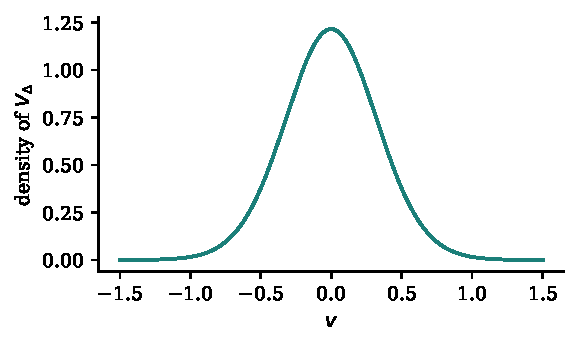
\includegraphics[width=0.75\textwidth]{figs/vdp_delta.pdf}
\caption{The density of $V_\Delta$, the inverse Fourier transform of $t\mapsto\Lambda(6,\Delta)/\Lambda(6+t,\Delta)$, computed from $L$ values for $|t|\le60$ only. It is positive, of mass $0.99995$, with value $1.21546$ at the origin, and log concave on the computed range.}\label{fig:10dvdp}
\end{figure}

For $\Delta$ the partner can be computed without knowing a single zero. We evaluated $g(t) = \Lambda(6,\Delta)/\Lambda(6+t,\Delta)$ on $0\le t\le60$ with PARI/GP and inverted the Fourier transform by quadrature. The result (Figure~\ref{fig:10dvdp}) is a positive density (minimum $2.4\cdot10^{-4}$ on $[0,1.5]$) of total mass $0.99995$, with density $1.21546$ at $0$, and log concave on the computed range. Log concavity is the P\'olya frequency property of order two, so the computation is numerical evidence for the two weakest consequences of Theorem~\ref{thm:10dvdp}(b).

\section{A gallery of van Dantzig pairs and Wald couples}

Each example below is a characteristic function $f$ with a partner $1/f(i\cdot)$ and, where available, a Wald couple. We checked every displayed identity numerically to at least nine digits.

\emph{Cosine and sine.} The function $\cos s = \prod_{k\ge1}(1-4s^2/((2k-1)\pi)^2)$ is the characteristic function of $\pm1$, with partner $1/\cosh s$, the characteristic function of $\sum_k2L_k/((2k-1)\pi)$. Similarly $\sin s/s$, the characteristic function of the uniform law on $(-1,1)$, has partner $s/\sinh s$, the characteristic function of $\sum_kL_k/(k\pi)$, and of the density $\frac\pi4\cosh^{-2}(\pi x/2)$. In the notation of Biane, Pitman and Yor \cite{bpy2001}, $\E e^{-\lambda C} = 1/\cosh\sqrt{2\lambda}$ and $\E e^{-\lambda S} = \sqrt{2\lambda}/\sinh\sqrt{2\lambda}$, so $(\pm1,C/2)$ and $(U,S/2)$, with $U$ uniform on $(-1,1)$, are Wald couples; $C$ and $S$ are hitting times of $1$ by the norms of one and three dimensional Brownian motion started at $0$.\index{Biane Pitman Yor variables}

\emph{Bessel functions and the symmetric Beta laws.} For $\nu>-\frac12$ let $X_\nu$ have the symmetric Beta (power semicircle) density $(1-x^2)^{\nu-1/2}/B(\nu+\frac12,\frac12)$ on $(-1,1)$: the arcsine law for $\nu=0$, the uniform law for $\nu=\frac12$, Wigner's semicircle for $\nu=1$, and the sign $\pm1$ as the limit $\nu\downarrow-\frac12$. Then
\begin{equation}\label{eq:10dbeta}
f_\nu(s) = \E e^{isX_\nu} = \Gamma(\nu+1)\Bigl(\frac s2\Bigr)^{-\nu}J_\nu(s) = \prod_{n\ge1}\Bigl(1-\frac{s^2}{j_{\nu,n}^2}\Bigr),
\end{equation}
with $j_{\nu,n}$ the positive zeros of $J_\nu$ (Exercise~\ref{ex:10dbeta}), and the partner $1/f_\nu(is) = \Gamma(\nu+1)^{-1}(s/2)^\nu/I_\nu(s)$ is the characteristic function of $H_\nu = \sum_nL_n/j_{\nu,n}$ \cite{hinds1974,jurek2010,amdeberhan2012,hasebesimonwang2018}. The case $\nu=\frac12$ is the sine pair above and $\nu=-\frac12$ the cosine pair. The Wald couple is $(X_\nu,T_\nu/2)$ with $T_\nu$ the hitting time of $1$ by a Bessel process of dimension $2\nu+2$ from $0$, whose Laplace transform $(\sqrt{2\lambda}/2)^\nu/(\Gamma(\nu+1)I_\nu(\sqrt{2\lambda}))$ is Kent's \cite{kent1978}.

\emph{Macdonald functions.} P\'olya \cite{polya1926} proved that for $a>0$ the function $t\mapsto K_{it}(a) = \int_0^\infty e^{-a\cosh u}\cos(tu)\,du$ has only real zeros. It is the Fourier transform of the positive even density proportional to $e^{-a\cosh u}$, so $t\mapsto K_{it}(a)/K_0(a)$ lies in $\mathcal D_L$ and $t\mapsto K_0(a)/K_t(a)$ is a characteristic function. Biane \cite{biane2009} gave a probabilistic account of P\'olya's theorem through matrix valued Brownian motion. The kernel $e^{-a\cosh u}$ is the simplest model of the P\'olya kernel of $\xi$, which behaves like $\exp(-\pi e^{2|u|})$.

\emph{Symmetric $z$ laws.} For $\delta>0$ let $G,G'$ be independent with the gamma law of shape $\delta$. Then $X = \log(G/G')$ has
\[
\E e^{isX} = \frac{|\Gamma(\delta+is)|^2}{\Gamma(\delta)^2} = \prod_{k\ge0}\Bigl(1+\frac{s^2}{(\delta+k)^2}\Bigr)^{-1},
\]
and for $\delta>\frac12$ its van Dantzig partner $\Gamma(\delta)^2/(\Gamma(\delta+t)\Gamma(\delta-t)) = \prod_{k\ge0}(1-t^2/(\delta+k)^2)$ is the characteristic function of $2\Theta$, where $\Theta$ has density proportional to $\cos^{2\delta-2}\theta$ on $(-\frac\pi2,\frac\pi2)$, by Cauchy's beta integral (we checked this at $\delta = 1.3$). So $X = \sqrt Y\,N$ is a normal variance mixture with mixing law $Y = \sum_{k\ge0}E_k/\lambda_k$, $\lambda_k = \frac12(\delta+k)^2$, a GGC with Thorin measure $\sum\delta_{\lambda_k}$. Partial fractions give the mixing density as an alternating series,
\[
p_Y(u) = \sum_{k\ge0}\binom{-2\delta}{k}\frac{\delta+k}{B(\delta,\delta)}\,e^{-(\delta+k)^2u/2},\qquad u>0,
\]
whose coefficients alternate in sign although $p_Y\ge0$. For $\delta=0.7$ we checked $\prod_k(1+s/\lambda_k)^{-1} = |\Gamma(\delta+i\sqrt{2s})|^2/\Gamma(\delta)^2$ to all printed digits at $s = 0.1$, $1$, $5$ (values $0.6076958543678661$, $0.04998906407585931$, $2.860474564093928\cdot10^{-4}$), and the Laplace transform of the series above against the product at $s=1.3$ to fifteen digits.

\emph{Gumbel and Hinds.} If $X = -\log E$, the Gumbel law with distribution function $\exp(-e^{-x})$, then
\[
\E e^{-sX} = \Gamma(1+s) = \exp\Bigl(-\gamma_{\mathrm E}s+\int_0^\infty(e^{-st}-1+st)\frac{dt}{t(e^t-1)}\Bigr),\qquad s>-1,
\]
with $\gamma_{\mathrm E}$ Euler's constant. The L\'evy density is $k(t)/t$ with $k(t) = 1/(e^t-1)$ completely monotone, so $X$ is an extended GGC in Bondesson's sense \cite{bondesson1992}. Hinds \cite{hinds1974} considered $X_1$ with density $\frac2{\sqrt\pi}\exp(x-e^{2x})$, that is $X_1 = \frac12\log G$ with $G$ of gamma law of shape $\frac12$, and $X_2 = -X_1$. Their characteristic functions are
\[
f_1(s) = \frac1{\sqrt\pi}\Gamma\Bigl(\frac{1+is}2\Bigr),\qquad f_2(s) = \frac1{\sqrt\pi}\Gamma\Bigl(\frac{1-is}2\Bigr),
\]
with normalisation $1/\sqrt\pi$, as $f_1(0)=1$ requires. Neither lies in $\mathcal D$: $Vf_1(t) = \sqrt\pi/\Gamma(\frac{1-t}2)$ is real but not even, while a real characteristic function is even. Their product, the characteristic function of $X_1-X_1'$ with $X_1'$ an independent copy of $X_1$, is $|\Gamma(\frac{1+is}2)|^2/\pi = 1/\cosh(\pi s/2)$ by the reflection formula, and $V(1/\cosh(\pi\cdot/2))(t) = \cos(\pi t/2)$: the cosine pair again.\index{Hinds pair}

\emph{The reciprocal Gamma function and a Gamma Wald couple.} Hartman \cite{hartman1976} proved that for real $c$ the function $e^{c\sqrt s}/\Gamma(1+\sqrt s)$ is the Laplace transform of a positive infinitely divisible law if and only if $c\le-\gamma_{\mathrm E}$ (see also \cite{roynetteyor2005}). Applying the sine squared lemma of the next section (Lemma~\ref{lem:10dsin2}) to $f=\Gamma$ at $\alpha=1$, whose L\'evy representation is the Gumbel formula above, gives the extreme case $c=-\gamma_{\mathrm E}$ with an explicit Thorin density (this book):
\begin{equation}\label{eq:10dnewman}
\frac{e^{-\gamma_{\mathrm E}\sqrt s}}{\Gamma(1+\sqrt s)} = \E e^{-sH_\Gamma},\qquad u_\Gamma(z) = \frac{\operatorname{Re}\psi(1+i\sqrt z)+\gamma_{\mathrm E}}{2\pi\sqrt z}\ge0,
\end{equation}
with $H_\Gamma$ a GGC of Thorin density $u_\Gamma$, where $\psi = \Gamma'/\Gamma$; positivity is the identity $\operatorname{Re}\psi(1+iy)+\gamma_{\mathrm E} = \sum_{k\ge1}y^2/(k(k^2+y^2))$. We checked \eqref{eq:10dnewman} at $s=2$ to nine digits. The GGC property is stated for the family $\Gamma(\alpha)e^{\sqrt s\,\psi(\alpha)}/\Gamma(\alpha+\sqrt s)$ in \cite{polson2018vdp}, Section~4; the density $u_\Gamma$ is computed here. Since $\E e^{s(\log E+\gamma_{\mathrm E})} = e^{\gamma_{\mathrm E}s}\Gamma(1+s)$, the pair $(\log E+\gamma_{\mathrm E},H_\Gamma)$ is a Wald couple with both members infinitely divisible: in our normalisation it is the couple that Roynette and Yor \cite{roynetteyor2005} build on Hartman's theorem.

\emph{Ostrovskii's hyperbolic class.} Ostrovskii \cite{ostrovskii1970} studied characteristic functions built from hyperbolic functions. In the form presented in the 2018 to 2021 versions of \cite{polson2018vdp}, one takes $f_\delta(z) = z^{-2}-(Cz)^{-1}+\delta\sum_ka_k/(z+h_k)$ with $\frac\pi2<C<B$, $h_k\ge B$, $a_k\ge0$, $\sum a_k<\infty$; then for $\delta$ small $\phi_\delta(t) = f_\delta(\cosh t)/f_\delta(1)$ and $1/\phi_\delta(it) = f_\delta(1)/f_\delta(\cos t)$ are both characteristic functions. The positivity of the Fourier transform of $\phi_\delta$ rests on the elementary integrals
\begin{align*}
\int_{\R}\frac{e^{itx}\,dt}{\cosh t+b} &= \frac{2\pi\sinh((\pi-a)x)}{\sin a\,\sinh\pi x}, & |b|<1,\ \cos a &= -b,\\
\int_{\R}\frac{e^{itx}\,dt}{\cosh t+b} &= \frac{2\pi\sin(ax)}{\sinh a\,\sinh\pi x}, & b>1,\ \cosh a &= b,
\end{align*}
and $\int e^{itx}\cosh^{-2}t\,dt = \pi x/\sinh(\pi x/2)$, which we verified (those versions misprint the second condition as $\cosh a = -b$). We refer to \cite{ostrovskii1970} for the precise class and do not reproduce the estimates.

\section{The sine squared transport}\index{sine squared transport}

The Thorin densities of this book have so far been read off from zeros. The following lemma, the $2\sin^2$ lemma of \cite{polson2018vdp} (Lemma~14 there; see also \cite{polson2017}, Section~5), produces them from the L\'evy measure of $\log f$ at a basepoint, which for an $L$ function is the arithmetic. Its first step, which writes $e^{-x\sqrt s}-1+x\sqrt s$ through the positive $\frac12$ stable law, is Th\'eor\`eme~I.1.1 of Roynette and Yor \cite{roynetteyor2005}, which also shows that the resulting $H$ is self decomposable. We state the lemma in our normalisation and prove it.

\begin{lemma}[sine squared lemma]\label{lem:10dsin2}
Let $f$ be holomorphic and zero free on $\operatorname{Re}w>\alpha-\eta$ for some $\eta>0$, positive on $(\alpha,\infty)$, and suppose that for $s\ge0$
\begin{equation}\label{eq:10dlk}
\log f(\alpha+s)-\log f(\alpha)-bs = \int_0^\infty(e^{-sx}-1+sx)\,\frac{\nu(dx)}x,\qquad b = \frac{f'(\alpha)}{f(\alpha)},
\end{equation}
with $\nu$ a positive measure on $(0,\infty)$ such that $\int_0^\infty\min(1,x)\,\nu(dx)<\infty$. Then for $s>0$
\[
\frac{f(\alpha)}{f(\alpha+\sqrt s)} = e^{-b\sqrt s}\,\E e^{-sH},
\]
where $H$ is a GGC with drift zero and Thorin density
\begin{equation}\label{eq:10dU}
U(z) = \frac1{2\pi\sqrt z}\int_0^\infty2\sin^2\Bigl(\frac{x\sqrt z}2\Bigr)\nu(dx) = \frac{\operatorname{Re}(f'/f)(\alpha+i\sqrt z)-b}{2\pi\sqrt z}.
\end{equation}
If $b\ge0$, $e^{-b\sqrt s}$ is the Laplace transform of a positive $\frac12$ stable law, a GGC with Thorin density $b/(2\pi\sqrt z)$, and then $f(\alpha)/f(\alpha+\sqrt s)$ is itself a GGC transform with Thorin density $\operatorname{Re}(f'/f)(\alpha+i\sqrt z)/(2\pi\sqrt z)$. The hypothesis \eqref{eq:10dlk} with $\nu\ge0$ holds if and only if $s\mapsto(\log f)''(\alpha+s)$ is completely monotone on $(0,\infty)$ and tends to $0$ at infinity.
\end{lemma}

\begin{proof}
\emph{Step 1: subordination.} For $x>0$ the positive $\frac12$ stable density $q_x(y) = \frac x{2\sqrt\pi}y^{-3/2}e^{-x^2/(4y)}$ has $\int_0^\infty e^{-sy}q_x(y)\,dy = e^{-x\sqrt s}$, and $\int_0^\infty(1-e^{-sy})y^{-3/2}dy = 2\sqrt\pi\sqrt s$ (substitute $u = sy$ and integrate by parts). Hence
\begin{align*}
e^{-x\sqrt s}-1+x\sqrt s &= \int_0^\infty(1-e^{-sy})\Bigl[\frac x{2\sqrt\pi}y^{-3/2}-q_x(y)\Bigr]dy\\
&= \int_0^\infty(1-e^{-sy})K(x,y)\,dy,
\end{align*}
with $K(x,y) = \frac x{2\sqrt\pi\,y^{3/2}}(1-e^{-x^2/(4y)})\ge0$.

\emph{Step 2: a Laplace pair.} For $a\ge0$ and $y>0$,
\begin{equation}\label{eq:10dpair}
\frac{1-e^{-a/y}}{\sqrt y} = \int_0^\infty e^{-yz}\,\frac{2\sin^2\sqrt{az}}{\sqrt{\pi z}}\,dz .
\end{equation}
Indeed $\int_0^\infty e^{-yz}(\pi z)^{-1/2}dz = y^{-1/2}$, and expanding the cosine,
\[
\int_0^\infty\frac{e^{-yz}\cos(2\sqrt{az})}{\sqrt{\pi z}}\,dz = \sum_{n\ge0}(-1)^n\frac{4^na^n\,\Gamma(n+\frac12)}{(2n)!\sqrt\pi\,y^{n+1/2}} = \frac{e^{-a/y}}{\sqrt y},
\]
using $\Gamma(n+\frac12) = (2n)!\sqrt\pi/(4^nn!)$; the interchange is justified by the bound $\cosh(2\sqrt{az})$ for the absolute series, which is integrable against $e^{-yz}z^{-1/2}$. Subtract and use $1-\cos2\theta = 2\sin^2\theta$.

\emph{Step 3: the L\'evy density.} Replace $s$ by $\sqrt s$ in \eqref{eq:10dlk} and insert Step 1. All integrands are nonnegative, so Tonelli's theorem gives
\[
\log\frac{f(\alpha+\sqrt s)}{f(\alpha)}-b\sqrt s = \int_0^\infty(1-e^{-sy})\frac{k(y)}y\,dy,
\]
with $k(y) = (4\pi y)^{-1/2}\int_0^\infty(1-e^{-x^2/(4y)})\,\nu(dx)$. By \eqref{eq:10dpair} with $a = x^2/4$ and Tonelli again, $k(y) = \int_0^\infty e^{-yz}U(z)\,dz$ with $U$ the first expression in \eqref{eq:10dU}. Frullani's integral $\int_0^\infty(1-e^{-sy})e^{-zy}y^{-1}dy = \log(1+s/z)$ then gives $\log(f(\alpha+\sqrt s)/f(\alpha))-b\sqrt s = \int_0^\infty\log(1+s/z)U(z)\,dz$, finite for each $s>0$. Finiteness for $s=1$ forces $\int_0^1|\log z|U(z)dz<\infty$ and $\int_1^\infty U(z)z^{-1}dz<\infty$, the integrability conditions of Definition~\ref{def:ch10ggc}, so $\exp(-\int\log(1+s/z)U(z)dz)$ is the transform of a GGC $H$.

\emph{Step 4: the closed form.} Differentiating \eqref{eq:10dlk}, $(f'/f)(\alpha+s)-b = \int_0^\infty(1-e^{-sx})\nu(dx)$ for $s>0$. The right side converges absolutely and uniformly for $\operatorname{Re}s\ge0$ because $|1-e^{-sx}|\le\min(2,|s|x)$, so it is continuous there and holomorphic inside; the left side is holomorphic on $\operatorname{Re}s>-\eta$. They agree for $\operatorname{Re}s\ge0$, and at $s = ir$ the real part of the right side is $\int(1-\cos rx)\nu(dx) = \int2\sin^2(rx/2)\nu(dx)$, which gives the second expression in \eqref{eq:10dU}.

\emph{Step 5.} $\int_0^\infty\log(1+s/z)z^{-1/2}dz = 2\pi\sqrt s$ (substitute $z = su$), so $b\sqrt s = \int\log(1+s/z)\,b(2\pi\sqrt z)^{-1}dz$, which is the stated GGC form of $e^{-b\sqrt s}$. Finally, \eqref{eq:10dlk} gives $(\log f)''(\alpha+s) = \int_0^\infty xe^{-sx}\nu(dx)$, completely monotone and tending to $0$. Conversely Bernstein's theorem writes such a function as $\int_{(0,\infty)}e^{-sx}m(dx)$ with $m\ge0$ and no atom at $0$; integrating twice from $0$ gives \eqref{eq:10dlk} with $\nu(dx) = m(dx)/x$.
\end{proof}

The second form of \eqref{eq:10dU} is Stieltjes inversion in disguise: on the cut $s = -z$ the principal root is $\sqrt s = i\sqrt z$. It shows that \emph{the transported Thorin density can be computed from $f$ alone on one vertical line}. The hypothesis $\nu\ge0$ is sufficient, not necessary, and fails for completed $L$ functions. The next theorem replaces it by a Hadamard argument.

\begin{theorem}[Shifted Thorin representation; this book, extending \cite{polson2017,polson2018vdp}]\label{thm:10dshift}
Let $\pi$ be as in Theorem~\ref{thm:10bmain}, or $\zeta$, and $a>0$. Put
\[
V_a(z) = \frac{\operatorname{Re}(\Xi_\pi'/\Xi_\pi)(a+i\sqrt z)}{2\pi\sqrt z},\qquad z>0 .
\]
\begin{enumerate}
\item[(i)] If every zero $z_k$ of $\Xi_\pi$ satisfies $|\operatorname{Re}z_k|<a$, then $V_a\ge0$ and $\Xi_\pi(a)/\Xi_\pi(a+\sqrt s) = \E e^{-sH_a}$ for $s>0$, with $H_a$ a GGC of drift zero and Thorin density $V_a$.
\item[(ii)] If $\Xi_\pi(a)/\Xi_\pi(a+\sqrt s)$ is a GGC transform on $(0,\infty)$, every zero satisfies $|\operatorname{Re}z_k|\le a$.
\item[(iii)] Unconditionally, (i) holds for every $a\ge\frac12$, that is for every basepoint $\alpha = \frac12+a\ge1$ in the variable $s$ of $\Lambda(s,\pi)$ in the unitary normalisation.
\item[(iv)] GRH for $\pi$ holds if and only if $V_a\ge0$ for every $a>0$, if and only if the conclusion of (i) holds for every $a>0$. Under GRH, $V_a(z)\,dz\to\sum_k\delta_{\gamma_k^2}$ vaguely and $H_a\to Z_\pi$ in law as $a\downarrow0$.
\end{enumerate}
\end{theorem}

\begin{proof}
(i) For $c\in\C$ with $\operatorname{Re}c>0$ and $s>0$, closing the contour in the lower half plane, where the only pole is $r = -i\sqrt s$,
\[
\frac1{2\pi}\int_{-\infty}^\infty\frac{dr}{(c+ir)(s+r^2)} = \frac1{2\sqrt s\,(c+\sqrt s)} .
\]
Taking real parts, and adding the same identity for $\bar c$, the integrand $\operatorname{Re}\frac1{c+ir}+\operatorname{Re}\frac1{\bar c+ir}$ is even in $r$ and positive, and the substitution $z = r^2$ gives
\[
\frac d{ds}\log\Bigl|1+\frac{\sqrt s}c\Bigr|^2 = \int_0^\infty\frac{v_c(z)\,dz}{s+z},
\]
with $v_c(z) = [\operatorname{Re}(c+i\sqrt z)^{-1}+\operatorname{Re}(\bar c+i\sqrt z)^{-1}]/(2\pi\sqrt z)>0$; for real $c>0$ use $c$ alone and halve. Integrating from $0$ (Tonelli) gives $\log|1+\sqrt s/c|^2 = \int_0^\infty\log(1+s/z)v_c(z)\,dz$. Now $\Xi_\pi(w) = \Xi_\pi(0)\prod_k(1-w^2/z_k^2)$, so
\[
\frac{\Xi_\pi(a+w)}{\Xi_\pi(a)} = \prod_k\Bigl(1+\frac w{a-z_k}\Bigr)\Bigl(1+\frac w{a+z_k}\Bigr),
\]
the product over pairs converging absolutely because each pair factor is $1+O((|w|+|w|^2)|z_k|^{-2})$. The numbers $c = a\mp z_k$ have positive real part by hypothesis and form a set closed under conjugation. Summing the single factor identities over this set (Tonelli), and halving because $c$ and $\bar c$ both occur, gives $\log(\Xi_\pi(a+\sqrt s)/\Xi_\pi(a)) = \int\log(1+s/z)V_a(z)\,dz$, because $\sum_c\operatorname{Re}(c+i\sqrt z)^{-1} = \operatorname{Re}\sum_k[(a+i\sqrt z-z_k)^{-1}+(a+i\sqrt z+z_k)^{-1}] = \operatorname{Re}(\Xi_\pi'/\Xi_\pi)(a+i\sqrt z)$. The integrability conditions follow as in Step 3 of Lemma~\ref{lem:10dsin2}.

(ii) By Lemma~\ref{lem:ch10nonvanish} the GGC transform $\varphi$ is holomorphic and zero free on $\C\setminus(-\infty,0]$, and $s\mapsto\Xi_\pi(a+\sqrt s)$ is holomorphic there; the identity $\varphi(s)\Xi_\pi(a+\sqrt s) = \Xi_\pi(a)$ on $(0,\infty)$ extends, so $\Xi_\pi(a+w)\ne0$ for $\operatorname{Re}w>0$. By evenness there is no zero with $\operatorname{Re}z<-a$.

(iii) By Lemma~\ref{lem:10bcompletion}(iii) all zeros satisfy $|\operatorname{Re}z_k|<\frac12$.

(iv) Under GRH, $\operatorname{Re}z_k = 0<a$ for all $k$, so (i) applies for every $a>0$. Conversely suppose $V_a\ge0$ for all $a>0$, and let $z_0$ be a zero of multiplicity $m$ with $\beta = \operatorname{Re}z_0>0$. For small $\eta\in(0,\beta)$, $(\Xi_\pi'/\Xi_\pi)(z_0-\eta) = -m/\eta+O(1)$, whose real part is negative; but $z_0-\eta = a+iy$ with $a = \beta-\eta>0$, and $V_a(y^2)\ge0$ says $\operatorname{Re}(\Xi'_\pi/\Xi_\pi)(a+iy)\ge0$ (for $y\ne0$; if $y=0$, then $z_0$ is real and the same argument applies to $(\Xi_\pi'/\Xi_\pi)(a)$, which is the limit of $\operatorname{Re}(\Xi'_\pi/\Xi_\pi)(a+iy)$ as $y\to0$). This contradiction and evenness give GRH; the second equivalence follows from (i) and (ii). For the limit, under GRH $\operatorname{Re}(\Xi_\pi'/\Xi_\pi)(a+ir) = \sum_{\gamma_k>0}[P_a(r-\gamma_k)+P_a(r+\gamma_k)]$ with the Poisson kernel $P_a(u) = a/(a^2+u^2)$, and $\frac1{2\pi r}P_a(r-\gamma)\,2r\,dr\to\delta_\gamma$ in the variable $r$, that is $\delta_{\gamma^2}$ in $z$; the terms $P_a(r+\gamma_k)$ tend to zero, uniformly summable. Convergence of the transforms, $\Xi_\pi(a)/\Xi_\pi(a+\sqrt s)\to\Xi_\pi(0)/\Xi_\pi(\sqrt s)$, gives convergence in law.
\end{proof}

For $\xi$, parts (i) to (iii) and the limit in (iv) are Theorem~18 and Remark~21 of \cite{polson2018vdp}, and \cite{polson2017} relates the family $\xi(\alpha)/\xi(\alpha+\sqrt s)$ to the criterion of Hinkkanen \cite{hinkkanen1997} and Lagarias \cite{lagarias1999}: the Riemann hypothesis holds if and only if $\operatorname{Re}\xi'/\xi(s)>0$ for $\operatorname{Re}s>\frac12$. Part (iv) is a Thorin form of that criterion. Parts (i) and (ii) are the parabolic picture of Section~\ref{sec:10bparabola} seen from a shifted basepoint: the Thorin property at $a$ is sandwiched between the conditions $\Theta_\sigma$ with $\sigma<a$ and $\sigma = a$. A zero $z_0 = \beta+i\gamma$ of $\Xi_\pi$ with $\beta>a$ would contribute \emph{locally} a negative dip to $V_a$ near $z = \gamma^2$, of depth about $(\beta-a)^{-1}/(2\pi\gamma)$. Chapter~\ref{ch:squarefree} splits these densities for $\xi$ into the contributions of single pairs of zeros, with a Brownian subordination (Corollary~\ref{cor:sf:sub}), Chapter~\ref{ch:beta} studies $V_a$ for $L(s,\chi_{-4})$, and Chapter~\ref{ch:scholze} computes the Thorin measure itself, as a signed density smoothed at width $\varepsilon$, by Stieltjes inversion. For self dual $\pi$, Chapter~\ref{ch:lap} writes $V_a$, halved by passing to $\Xi^{\mathrm{sd}}_\pi$, in the variable $r=\sqrt z$, as a superposition over the zeros of folded Cauchy laws of scales $a-\beta$, so that moving the basepoint adds Cauchy noise (Theorem~\ref{thm:lapcauchy}).

\subsection{At the centre: from the cosine measure to the zeros}

Formally, for real $\gamma>0$ and $\operatorname{Re}z>0$, Frullani's integral with an Abel damping gives
\begin{align*}
\log\Bigl(1+\frac{z^2}{\gamma^2}\Bigr) &= \lim_{\epsilon\downarrow0}2\int_0^\infty\bigl(e^{-\epsilon x}-e^{-(z+\epsilon)x}\bigr)\cos(\gamma x)\frac{dx}x\\
&= \int_0^\infty(1-e^{-zx})\,2\cos(\gamma x)\frac{dx}x,
\end{align*}
so that under GRH, $\log(\Xi_\pi(z)/\Xi_\pi(0)) = -\int_0^\infty(e^{-zx}-1+zx)\mu(dx)/x$ formally, with the \emph{cosine L\'evy measure}\index{cosine L\'evy measure} $\mu(dx) = 2\sum_k\cos(\gamma_kx)\,dx$ (the linear term vanishes because $\Xi_\pi'(0) = 0$). Insert $-\mu$ for $\nu$ in the first form of \eqref{eq:10dU} at $\alpha = 0$. As distributions in $r = \sqrt z>0$, we have $\int_0^\infty\cos(\gamma x)dx = 0$ and $\int_0^\infty\cos(rx)\cos(\gamma x)dx = \frac\pi2\delta(r-\gamma)$, so
\begin{align*}
U(z) &= -\frac1{2\pi r}\sum_k2\int_0^\infty(1-\cos rx)\cos(\gamma_kx)\,dx\\
&= \frac1{2r}\sum_k\delta(r-\gamma_k) = \sum_k\delta(z-\gamma_k^2),
\end{align*}
using $\delta(\sqrt z-\gamma) = 2\gamma\,\delta(z-\gamma^2)$. \emph{The sine squared transport carries the cosine measure of the zeros exactly to the Thorin measure $\sum_k\delta_{\gamma_k^2}$.} The damping $e^{-\epsilon x}$ makes this rigorous: it is the shift $a = \epsilon$, and the computation becomes Theorem~\ref{thm:10dshift}.

\begin{proposition}[this book]\label{prop:10dsmooth}
Assume GRH for $\pi$ and let $\epsilon>0$. With $P_\epsilon(u) = \epsilon/(\epsilon^2+u^2)$ and $b_\epsilon = (\Xi_\pi'/\Xi_\pi)(\epsilon) = \sum_{\gamma_k>0}2P_\epsilon(\gamma_k)$,
\begin{gather*}
\frac{\Xi_\pi(\epsilon)}{\Xi_\pi(\epsilon+\sqrt s)} = e^{-b_\epsilon\sqrt s}\exp\Bigl(-\int_0^\infty\log\Bigl(1+\frac sz\Bigr)U_\epsilon(z)\,dz\Bigr),\\
U_\epsilon(z) = \frac1{2\pi\sqrt z}\sum_{\gamma_k>0}\bigl[P_\epsilon(\sqrt z-\gamma_k)+P_\epsilon(\sqrt z+\gamma_k)-2P_\epsilon(\gamma_k)\bigr],
\end{gather*}
and $U_\epsilon(z) = (2\pi\sqrt z)^{-1}\int_0^\infty2\sin^2(x\sqrt z/2)e^{-\epsilon x}(-\mu)(dx)$ is the sine squared transport of the damped cosine measure.
\end{proposition}

\begin{proof}
$U_\epsilon = V_\epsilon-b_\epsilon/(2\pi\sqrt z)$ in the notation of Theorem~\ref{thm:10dshift}, and the identity is (i) of that theorem combined with Step 5 of Lemma~\ref{lem:10dsin2}. The transport formula is the elementary integral $\int_0^\infty(1-\cos rx)\cos(\gamma x)e^{-\epsilon x}dx = P_\epsilon(\gamma)-\frac12[P_\epsilon(r-\gamma)+P_\epsilon(r+\gamma)]$, summed over $k$.
\end{proof}

\begin{figure}[t]
\centering
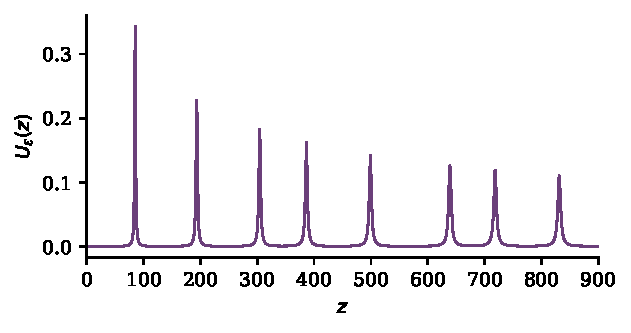
\includegraphics[width=0.78\textwidth]{figs/sin2_transport.pdf}
\caption{The sine squared transport $U_\epsilon(z)$ of the damped cosine L\'evy measure $2\sum_k\cos(\gamma_kx)e^{-0.05x}$ over the first $60$ zeros of $\Delta$: a smoothed Thorin density with peaks at $\gamma_k^2$, mass $0.983$ within $30$ of $\gamma_1^2 = 85.052$.}\label{fig:10dsin2}
\end{figure}

For $\Delta$, with $\epsilon = 0.05$ and the first $60$ zeros, $U_\epsilon$ is positive on $4\le z\le900$ (minimum $2.0\cdot10^{-5}$) with peaks at the $\gamma_k^2$ and mass $0.983$ within $30$ of $\gamma_1^2 = 85.052$, unit mass up to the smoothing loss (Figure~\ref{fig:10dsin2}). Since $U_\epsilon$ contains the negative term $-b_\epsilon/(2\pi\sqrt z)$, its positivity is a property of the zeros and not of the construction.

\subsection{The explicit formula: from the primes to the Thorin measure}\index{explicit formula}

The cosine measure is the Fourier transform of the zero counting measure, and Weil's explicit formula (Theorem~\ref{thm:10cexplicit} for $\Delta$; \cite{weil1952,iwanieckowalski2004} in general) computes that transform. Let $\pi$ be self dual with $\Lambda(\frac12,\pi)\ne0$, and write $-L'/L(s,\pi) = \sum_n\Lambda_\pi(n)n^{-s}$ in the unitary normalisation. Taking for $h$ the cosine kernel, the formula reads, as an identity of distributions on $(0,\infty)$,
\begin{equation}\label{eq:10dweil}
\mu(dx) = 2\sum_{\gamma_k>0}\cos(\gamma_kx)\,dx = -\sum_{n\ge2}\frac{\Lambda_\pi(n)}{\sqrt n}\,\delta_{\log n}(dx)+A_\pi(x)\,dx,
\end{equation}
where $A_\pi$ is the archimedean density, the Fourier transform of $\frac1{2\pi}2\operatorname{Re}[\frac{\gamma'}{\gamma}(\frac12+it,\pi)]$; for $\zeta$ the right side also contains the polar term $2\cosh(x/2)\,dx$. Combining \eqref{eq:10dweil} formally with the transport: \emph{the Thorin density of $1/F_\pi$ is the sine squared transform of the explicit formula distribution, and GRH is its positivity.} Since the transport acts on $\nu = -\mu$, the atom at $\log n$ contributes $+\Lambda_\pi(n)n^{-1/2}(2\pi\sqrt z)^{-1}2\sin^2(\frac12\sqrt z\log n)$, of the sign of $\Lambda_\pi(n)$, and for $\Delta$ the atoms of \eqref{eq:10dweil} at $\log p^m$, $m\ge1$, are, up to sign and the factor $p^{-m/2}$, the corresponding atoms of the Fourier transform of the local Thorin comb of $p$ (Proposition~\ref{prop:10cdictionary}); only the sum over all $n$ together with $A_\pi$ is concentrated on the $\gamma_k^2$.\index{heat trace}

The rigorous form of this statement uses test functions. The heat trace
\[
\mathcal W_\pi(x) = k_\pi(x) = \sum_ke^{-x\gamma_k^2},
\]
summed over the pairs $\pm z_k = \pm i\gamma_k$ of \eqref{eq:10batoms}, formed from $\Xi^{\mathrm{sd}}_\pi$ when $\pi$ is self dual, so that each zero of $\Lambda(s,\pi)$ counts once, as in Table~\ref{tab:10dheat}, is the L\'evy function of Theorem~\ref{thm:10bmain}(d), so \emph{GRH holds if and only if $\mathcal W_\pi$ is completely monotone}. For $\xi$ the first author states in \cite{polson2018vdp} (Theorems~22 and~26) that the heat trace is positive and strictly decreasing unconditionally, so that the law with Laplace transform $\xi(\frac12)/\xi(\frac12+\sqrt s)$ is self decomposable, and that its complete monotonicity is equivalent to the Riemann hypothesis; the second statement is the case $\pi = \zeta$ of Theorem~\ref{thm:10bmain}, and we do not use the first. With $h(t) = t^{2n}e^{-xt^2}$ in Weil's formula, $(-1)^n\mathcal W^{(n)}(x) = \sum\gamma_k^{2n}e^{-x\gamma_k^2}$ is a sum over primes plus an archimedean integral. Since the transform $H(y)$ of $h$ in Theorem~\ref{thm:10cexplicit} then decays like $e^{-y^2/(4x)}$, only primes with $\log p\le\sqrt{240x}+1$ matter at double precision: $p\le24$ at $x = 0.02$ and $p\le365$ at $x = 0.1$. For $\Delta$ we obtained, from the zeros and independently from the primes, the values in Table~\ref{tab:10dheat}: agreement to thirteen to sixteen significant digits, with the complete monotonicity signs through $n=3$. Small $x$ needs only a few primes and is dominated by the archimedean term; large $x$ and high derivative orders need many primes, and that is where individual ordinates are resolved.

\begin{table}[t]
\centering\footnotesize
\begin{tabular}{llll}
\toprule
$x$ & quantity & from the zeros & from the primes\\
\midrule
$0.02$ & $\mathcal W$ & $0.2061515276408161$ & $0.20615152764081612$\\
 & $-\mathcal W'$ & $20.450633094275233$ & $20.450633094275236$\\
 & $\mathcal W''$ & $2391.2851645202795$ & $2391.2851645202795$\\
 & $-\mathcal W'''$ & $359738.32402760646$ & $359738.3240276065$\\
$0.05$ & $\mathcal W$ & $0.014290332953786858$ & $0.01429033295378686$\\
 & $-\mathcal W'''$ & $9216.990197017574$ & $9216.99019701757$\\
$0.1$ & $\mathcal W$ & $2.0241135580126968\cdot10^{-4}$ & $2.0241135580125608\cdot10^{-4}$\\
 & $-\mathcal W'''$ & $124.56174145637718$ & $124.56174145637709$\\
\bottomrule
\end{tabular}
\caption{The heat trace $\mathcal W(x) = \sum_{\gamma>0}e^{-x\gamma^2}$ of $\Delta$ and its derivatives, from the zeros and from the primes through Weil's explicit formula.}\label{tab:10dheat}
\end{table}

Figure~\ref{fig:10dheatfig} plots the same quantities as functions of $x$.

\begin{figure}[ht]\centering
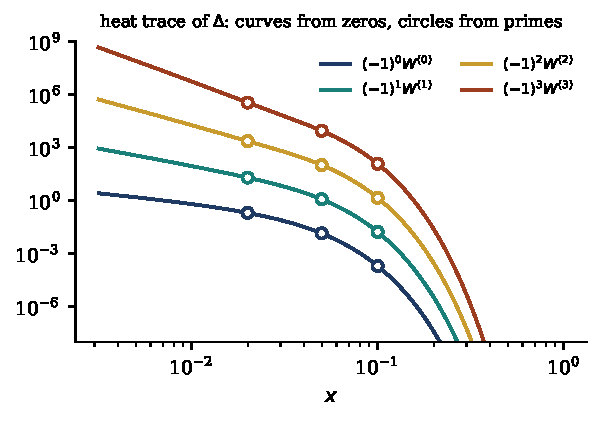
\includegraphics[width=0.9\textwidth]{figs/heattrace_primes.pdf}
\caption{Heat trace $\mathcal W$ of $\Delta$ and its first three derivatives with alternating signs. Curves: sums over the zeros up to height 300. Circles: Weil's explicit formula, using only the primes and the archimedean term. Complete monotonicity is the statement that every such curve is positive for every $n$.}\label{fig:10dheatfig}
\end{figure}

\begin{figure}[t]
\centering
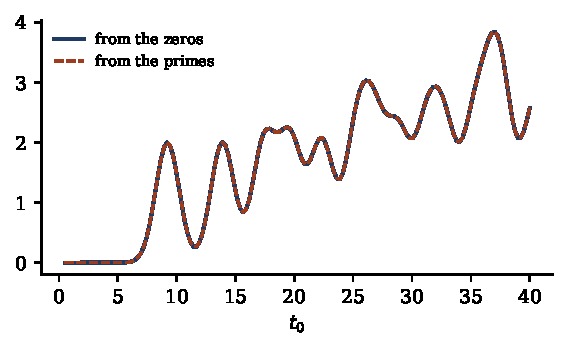
\includegraphics[width=0.78\textwidth]{figs/zeros_from_primes.pdf}
\caption{Zeros from primes for $\Delta$: the smoothed zero count $\sum_{\gamma}[e^{-(\gamma-t_0)^2/2}+e^{-(\gamma+t_0)^2/2}]$ from the zeros and from the primes $p\le1.6\cdot10^5$ with the archimedean term. Maximal difference $4.0\cdot10^{-14}$ for $t_0\in[0.5,40]$.}\label{fig:10dprimes}
\end{figure}

The same mechanism recovers the zeros themselves: in Figure~\ref{fig:10dprimes} the smoothed zero count of $\Delta$ computed from the primes agrees with that computed from the zeros to $4.0\cdot10^{-14}$, against a peak value of $3.84$.

\subsection{Away from the centre}\label{sec:10daway}

For $\alpha>1$ the Euler product gives the L\'evy measure of $\log L(\alpha+s,\pi)$ explicitly:
\[
\log\frac{L(\alpha+s,\pi)}{L(\alpha,\pi)}-s\frac{L'}L(\alpha,\pi) = \sum_{n\ge2}\frac{\Lambda_\pi(n)}{n^\alpha\log n}\bigl(e^{-s\log n}-1+s\log n\bigr),
\]
so $\nu_{\mathrm{ar}} = \sum_n\Lambda_\pi(n)n^{-\alpha}\delta_{\log n}$, whose transport is
\[
U_{\mathrm{ar}}(z) = \frac1{2\pi\sqrt z}\sum_{n\ge2}\frac{\Lambda_\pi(n)}{n^\alpha}\,2\sin^2\Bigl(\frac{\sqrt z\log n}2\Bigr).
\]
Chapter~\ref{ch:lap} inverts this transport, signed or not, by Gaussian means and recovers the $\Lambda_\pi(n)$ (Corollary~\ref{cor:lapfrob}). For $\zeta$, for Dedekind zeta functions and for the Rankin Selberg function $L(s,\pi\times\tilde\pi)$, either partial, as $L^S$ with $S$ a finite set of primes containing the ramified ones, or complete (Theorem~\ref{thm:ch09rs} and the paragraph after it), the coefficients $\Lambda_\pi(n)$ are nonnegative, so $U_{\mathrm{ar}}\ge0$. The completed function adds two archimedean pieces of opposite sign. Binet's formula $(\log\Gamma)''(w) = \int_0^\infty te^{-wt}(1-e^{-t})^{-1}dt$ shows that $\log\Gamma((\alpha+s)/2)$ contributes the positive density $e^{-\alpha x}(1-e^{-2x})^{-1}$ to $\nu$, while Frullani's integral shows that the polynomial factors $s(s-1)$ of $\xi$ contribute $-(e^{-\alpha x}+e^{-(\alpha-1)x})$, a negative density. Hence $\nu$ is a signed measure for $\xi$ and Lemma~\ref{lem:10dsin2} does not apply as stated; what must be checked is the positivity of the \emph{total} transported density. The first author discusses this decomposition in \cite{polson2018vdp} (Remark~19) and obtains the Thorin representation of $\xi(\alpha)/\xi(\alpha+\sqrt s)$ for $\alpha\ge1$ from the Hadamard product instead, as Theorem~\ref{thm:10dshift}(iii) does for every $\Xi_\pi$. For signed coefficients, as for $L(s,\chi)$ with $\chi$ real taking the value $-1$, or $L(s,\Delta)$, the arithmetic part $\nu_{\mathrm{ar}}$ is itself signed, and for complex $\chi$ it is complex; one must then work with the completion $\Xi_\chi$ of Chapter~\ref{ch:10b}. Inside the critical strip the question is of Riemann hypothesis type: by the argument of Theorem~\ref{thm:10dshift}(iv), nonnegativity of $V_{a'}$ for every $a'\ge a$ excludes zeros of $\Lambda(s,\pi)$ with real part above $\frac12+a$.

We computed the density $U$ of \eqref{eq:10dU}, in its second form, at the $15000$ points $\sqrt z=0.01,0.02,\dots,150$, for $\xi$ at $\alpha = 0.55, 0.75, 0.99, 1.25, 2$ and for $\Delta$ at the basepoints $6+\alpha-\frac12$ of $\Lambda(s,\Delta)$, the same offsets $\alpha-\frac12$ from the centre; it is positive at every point in every case, with its minimum at $\sqrt z=0.01$, where $U$ vanishes like a multiple of $\sqrt z$ (the value there is $1.8\cdot10^{-8}$ for $\xi$ at $\alpha = 0.55$ and $9.5\cdot10^{-8}$ for $\Delta$ at the same $\alpha$). These are numerical observations at every $\alpha$, and the grid sees only zeros of height below $150$. For $\alpha\ge1$, Theorem~\ref{thm:10dshift}(iii) proves only $V_{\alpha-1/2}\ge0$; since $U = V_{\alpha-1/2}-b/(2\pi\sqrt z)$ with $b>0$, positivity of $U$ is a stronger statement: for $\xi$ it says that $\operatorname{Re}\xi'/\xi$ is smallest on the real axis along the line $\operatorname{Re}s=\alpha$. Lagarias \cite{lagarias1999} proved this under the Riemann hypothesis for every $\alpha>\frac12$, and unconditionally for $\alpha\ge10$; Garunk\v{s}tis lowered the unconditional range to $\alpha>4.5$ \cite{garunkstis2000} and then to $\alpha\ge1$ \cite{garunkstis2002}. Unconditionally it is open only for $\frac12<\alpha<1$, where Chapter~\ref{ch:beta} proves it up to the height to which the Riemann hypothesis is verified, with the analogue for $L(s,\chi_{-4})$ (Theorem~\ref{beta:thm:minall}). Chapter~\ref{ch:recip} builds the corresponding family for the Rankin Selberg square of an Artin representation from its Frobenius traces, keeping the poles of the completed $L$ function, so that no polynomial factor contributes a negative density; there the densities are nonnegative for $\alpha>1$ (Proposition~\ref{prop:recipfamily}), and below $\alpha=1$ the same question is Open Problem~\ref{op:recipdescent}.

\section{Subordinators of L functions and hitting times}\index{zeta subordinator}

Fix $\sigma>1$. Since $\log\zeta(\sigma+\lambda)-\log\zeta(\sigma) = -\sum_{n\ge2}\frac{\Lambda(n)}{n^\sigma\log n}(1-n^{-\lambda})$, the function $\lambda\mapsto\log(\zeta(\sigma)/\zeta(\sigma+\lambda))$ is a Bernstein function with L\'evy measure $\Pi_\sigma = \sum_n\frac{\Lambda(n)}{n^\sigma\log n}\delta_{\log n}$ of total mass $\log\zeta(\sigma)$. Let $X_t$ be the compound Poisson subordinator with this L\'evy measure:
\[
\E e^{-\lambda X_t} = \Bigl(\frac{\zeta(\sigma+\lambda)}{\zeta(\sigma)}\Bigr)^t,\qquad\lambda\ge0,\ t\ge0 .
\]
Let $d_t(m)$ be the Dirichlet coefficients of $\zeta^t$, defined as $\exp(t\log\zeta)$: $d_t$ is multiplicative with $d_t(p^k) = \binom{t+k-1}k$.

\begin{proposition}[this book]\label{prop:10dsublaw}
For $t>0$, $X_t$ takes values in $\{\log m:m\ge1\}$ and $\Prob(X_t = \log m) = d_t(m)m^{-\sigma}/\zeta(\sigma)^t$.
\end{proposition}

\begin{proof}
The jumps of $X$ lie in $\{\log n\}$, so $X_t$ is the logarithm of a product of integers. For $\operatorname{Re}s>1$ the Euler product gives
\[
\zeta(s)^t = \prod_p(1-p^{-s})^{-t} = \prod_p\sum_k\binom{t+k-1}kp^{-ks} = \sum_md_t(m)m^{-s},
\]
with $d_t(m)\ge0$. Hence $\E e^{-\lambda X_t} = \sum_m d_t(m)m^{-\sigma}\zeta(\sigma)^{-t}e^{-\lambda\log m}$ for $\lambda\ge0$, and the coefficients sum to $1$ at $\lambda = 0$. A law on $[0,\infty)$ is determined by its Laplace transform.
\end{proof}

As $\sigma\downarrow1$ the ranked normalised sizes of the prime factors of the integer $e^{X_t}$ converge in law to the Poisson Dirichlet law with parameter $t$ (Theorem~\ref{thm:pdtheta}), so that the zeta subordinator carries the whole Ewens family.

Let $c>0$ and $Z_t = t/c-X_t$, a spectrally negative L\'evy process of bounded variation with drift $1/c$. Its Laplace exponent $\psi(\lambda) = \log\E e^{\lambda Z_1} = \lambda/c+\log(\zeta(\sigma+\lambda)/\zeta(\sigma))$ is convex on $[0,\infty)$ with $\psi(0)=0$ and $\psi(\lambda)\to\infty$; let $\Phi$ be its right inverse. Let $\tau_x = \inf\{t:Z_t>x\}$ for $x>0$. Since $Z$ moves up only continuously, $Z_{\tau_x} = x$ on $\{\tau_x<\infty\}$, so
\[
\tau_x = c\bigl(x+\log M_x\bigr),\qquad M_x = e^{X_{\tau_x}}\in\{1,2,3,\dots\}.
\]
We use two classical facts: $\E e^{-q\tau_x} = e^{-x\Phi(q)}$ for $q\ge0$ \cite{bertoin1996,kyprianou2014}, and Kendall's identity \cite{kendall1957,bertoin1996,kyprianou2014}: for a spectrally negative L\'evy process $Z$ that is not the negative of a subordinator, as measures on $(0,\infty)^2$,
\begin{equation}\label{eq:10dkendall}
t\,\Prob(\tau_x\in dt)\,dx = x\,\Prob(Z_t\in dx)\,dt .
\end{equation}
In outline, for compound Poisson $X$, \eqref{eq:10dkendall} is a consequence of Tak\'acs' ballot theorem \cite{takacs1967}: if $S$ is a nondecreasing step process with cyclically exchangeable increments on $[0,t]$ and $S_0 = 0$, then $\Prob(S_u<u/c\text{ for all }u\in(0,t]\mid S_t = y) = (1-cy/t)^+$. Applying it to the time reversal $S_u = X_t-X_{(t-u)-}$, which has the same law as $X$ on $[0,t]$, the event that $Z$ first exceeds level $x = t/c-y$ at time $t$ is the event that the reversed path stays strictly below the line $u/c$, and its conditional probability $x/(t/c)$ given $X_t = y$ is \eqref{eq:10dkendall} after the change of variables $x = t/c-y$. We refer to \cite{bertoin1996}, Chapter~VII, for the general case.

\begin{theorem}[First passage law; this book]\label{thm:10dballot}
Let $\sigma>1$, $c>0$, $x>0$. For every integer $m\ge1$,
\[
\Prob(M_x = m) = \frac x{x+\log m}\cdot\frac{d_t(m)\,m^{-\sigma}}{\zeta(\sigma)^t},\qquad t = c(x+\log m),
\]
and $\sum_m\Prob(M_x = m)\,e^{-qc(x+\log m)} = e^{-x\Phi(q)}$. If $1/c\ge-\zeta'/\zeta(\sigma)$, then $\tau_x<\infty$ almost surely.
\end{theorem}

\begin{figure}[ht]\centering
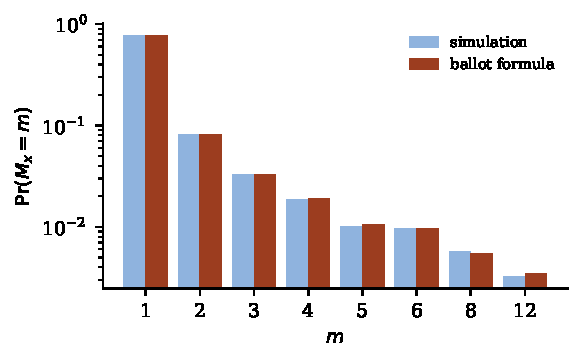
\includegraphics[width=0.8\textwidth]{figs/zeta_passage.pdf}
\caption{First passage law of the zeta subordinator ($\sigma=2$, $c=1/2$, $x=1$): simulation of $200000$ paths against the ballot formula of Theorem~\ref{thm:10dballot}.}\label{fig:10dpassage}
\end{figure}

\begin{proof}
By Proposition~\ref{prop:10dsublaw}, $\Prob(Z_t\in dx)\,dt = \sum_mp_t(m)\,\delta_{t/c-\log m}(dx)\,dt$ with $p_t(m) = d_t(m)m^{-\sigma}\zeta(\sigma)^{-t}$. On the line $\{t = c(x+\log m)\}$, parametrised by $x$, the measure $\delta_{t/c-\log m}(dx)\,dt$ is $c\,dx$. On the other side, $\Prob(\tau_x\in dt)\,dx = \sum_m\Prob(M_x = m)\,\delta_{c(x+\log m)}(dt)\,dx$. Distinct $m$ give disjoint lines, so \eqref{eq:10dkendall} gives $t\,\Prob(M_x = m) = x\,c\,p_t(m)$ with $t = c(x+\log m)$, which is the formula. The Laplace transform identity is $\E e^{-q\tau_x} = e^{-x\Phi(q)}$ written out. Finally $\psi'(0+) = 1/c+\zeta'/\zeta(\sigma)$; if it is nonnegative, $\Phi(0) = 0$ and $\Prob(\tau_x<\infty) = e^{-x\Phi(0)} = 1$.
\end{proof}

The theorem is a Lagrange inversion for Dirichlet series: summing over $m$ at $q = 0$ gives $\sum_m\frac x{x+\log m}d_{c(x+\log m)}(m)m^{-\sigma}\zeta(\sigma)^{-c(x+\log m)} = 1$ under the drift condition. We simulated $200000$ paths with $\sigma = 2$, $c = 0.5$, $x = 1$ (so $1/c = 2>-\zeta'/\zeta(2) = 0.5700$) and compared with the formula (Figure~\ref{fig:10dpassage}):

\begin{center}\small
\begin{tabular}{lcccccc}
\toprule
$m$ & $1$ & $2$ & $3$ & $4$ & $6$ & $12$\\
\midrule
simulation & $0.78075$ & $0.08160$ & $0.03273$ & $0.01873$ & $0.00970$ & $0.00324$\\
Theorem~\ref{thm:10dballot} & $0.77970$ & $0.08202$ & $0.03296$ & $0.01892$ & $0.00968$ & $0.00349$\\
\bottomrule
\end{tabular}
\end{center}

\noindent All differences are within two standard errors.

The construction needs only that $\log L$ has nonnegative Dirichlet coefficients, so it applies verbatim to a Dedekind zeta function $\zeta_K$, with values in $\{\log\mathrm N\mathfrak a\}$, and to $L(s,\pi\times\tilde\pi)$, partial or complete (Theorem~\ref{thm:ch09rs} and the paragraph after it), whose subordinator is the probabilistic object attached to $\pi$ to the right of $1$. It fails for $L(s,\chi)$ when $\chi$ takes the value $-1$ and for $L(s,\Delta)$, whose L\'evy measures are signed as in~\eqref{eq:ch09signed}: at $t=1$ the candidate weights $\chi(m)m^{-\sigma}/L(\sigma,\chi)$ take negative values, and even $L(s,\chi)L(s,\bar\chi)$, whose coefficient at $p^k$ is $2\operatorname{Re}\chi(p)^k/k$, does not suffice.\index{Kendall's identity}\index{ballot theorem}

\section{The Patie class}\index{Patie class}\index{Bernstein gamma function}

Patie and Savov \cite{patiesavov2018} introduced \emph{Bernstein gamma functions}: for a Bernstein function $\phi$, $W_\phi$ is the unique solution, in a suitable class, of
\[
W_\phi(z+1) = \phi(z)W_\phi(z),\qquad W_\phi(1) = 1,
\]
so that $W_\phi(n+1) = \phi(1)\cdots\phi(n)$ and $W_\phi = \Gamma$ for $\phi(z) = z$. They govern exponential functionals of L\'evy processes: for a subordinator $\eta$ with Laplace exponent $\phi$, the exponential functional $I_\phi = \int_0^\infty e^{-\eta_t}dt$ has $\E I_\phi^{\,n} = n!/W_\phi(n+1)$, and Patie and Savov extend this to the Mellin transform, $\E I_\phi^{\,z-1} = \Gamma(z)/W_\phi(z)$. Konstantopoulos, Patie and Sarkar use them to build a new class of van Dantzig solutions. Let $\Psi$ be the Laplace exponent of a possibly killed spectrally negative L\'evy process,
\[
\Psi(u) = -\kappa+au+\tfrac12\sigma^2u^2-\int_0^\infty\bigl(1-e^{-ur}-ur\mathrm{1}_{\{r<1\}}\bigr)\Pi(dr),
\]
with $\kappa\ge0$, $\sigma^2\ge0$, $\int_0^\infty\min(1,r^2)\,\Pi(dr)<\infty$, excluding the degenerate case in which the process is the negative of a subordinator, and with $\Psi(\frac12)\ge0$ (equivalently, the largest zero of $\Psi$ in $[0,\infty)$ lies in $[0,\frac12]$). Put
\[
J_\Psi(t) = \sum_{n\ge0}\frac{(-1)^nt^{2n}}{W_\Psi(n+1)},\qquad W_\Psi(n+1) = \Psi(1)\cdots\Psi(n),\qquad\mathcal D_P = \{J_\Psi\}.
\]

\begin{theorem}[Konstantopoulos, Patie and Sarkar \cite{konstantopoulospatiesarkar2024}, Theorem~4.1 and Lemma~5.7]\label{thm:10dpatie}
$\mathcal D_P\subset\mathcal D$. The partner $1/J_\Psi(i\cdot)$ is the characteristic function of $D_\Psi = \sqrt2\,B_{T_\Psi}$, where $B$ is a Brownian motion and $T_\Psi$ an independent positive self decomposable variable. The Bessel functions of \eqref{eq:10dbeta} are the case $\Psi(u) = u(u+\nu)$, up to the scaling $t\mapsto2t$.
\end{theorem}

They leave open whether $t\mapsto\xi(\frac12+it)/\xi(\frac12)$ lies in $\mathcal D_P$, noting that the question does not seem straightforward. We give a necessary condition that can be tested from Taylor coefficients.

\begin{proposition}[this book]\label{prop:10dpatietest}
Let $\Xi_\pi(z) = \sum_{n\ge0}a_nz^{2n}$ with all $a_n>0$, and suppose $\Xi_\pi(it)/\Xi_\pi(0) = J_\Psi(t)$ for some $\Psi$ as above. Then $\Psi(n) = a_{n-1}/a_n$ for $n\ge1$, and the sequence $\delta_n = \Psi(n+2)-2\Psi(n+1)+\Psi(n)$ is completely monotone in the sense of Hausdorff:
\[
(-1)^k\Delta^k\delta_n\ge0\qquad\text{for all }k\ge0,\ n\ge1,
\]
where $\Delta\delta_n = \delta_{n+1}-\delta_n$.
\end{proposition}

\begin{proof}
Comparing coefficients of $t^{2n}$ in $\sum(-1)^na_nt^{2n}/a_0$ and $J_\Psi(t)$ gives $W_\Psi(n+1) = a_0/a_n$, so $\Psi(n) = W_\Psi(n+1)/W_\Psi(n) = a_{n-1}/a_n$. For $u>0$ differentiation under the integral, justified by $\int\min(1,r^2)\Pi(dr)<\infty$ and the bound $r^2e^{-ur}\le C_u\min(1,r^2)$, gives $\Psi''(u) = \sigma^2+\int_0^\infty r^2e^{-ur}\Pi(dr)$. Hence
\[
\delta_n = \int_0^1\!\!\int_0^1\Psi''(n+u+v)\,du\,dv = \sigma^2+\int_0^\infty e^{-nr}(1-e^{-r})^2\,\Pi(dr),
\]
which is $\int_{[0,1]}y^n\,\rho(dy)$, where $\rho$ is the image of $(1-e^{-r})^2\Pi(dr)$ under $y = e^{-r}$ plus the atom $\sigma^2\delta_1$, a finite positive measure because $(1-e^{-r})^2\le\min(1,r^2)$. Then $(-1)^k\Delta^k\delta_n = \int y^n(1-y)^k\rho(dy)\ge0$.
\end{proof}

\begin{table}[t]
\centering\footnotesize
\setlength{\tabcolsep}{2.5pt}
\begin{tabular}{lrrrrrl}
\toprule
completed $L$ function & $d$ & $N$ & $\Psi(1)$ & $\Psi(2)$ & $\Psi(3)$ & Hausdorff test\\
\midrule
$\xi$ & 1 & 1 & 43.2807 & 93.0400 & 148.3165 & no violation, $k\le30$\\
$L(s,\chi_{-4})$ & 1 & 4 & 12.8181 & 30.2532 & 51.2721 & no violation, $k\le30$\\
$\Delta$ & 2 & 1 & 17.8012 & 38.0083 & 60.2084 & no violation, $k\le30$\\
$L(s,\chi_{-3})$ & 1 & 3 & 17.6363 & 39.5190 & 65.1347 & fails: $k=5$, $n=1$, $-1.24\cdot10^{-3}$\\
$L(s,\chi_5)$ & 1 & 5 & 12.7458 & 28.8566 & 47.9351 & fails: $k=7$, $n=3$, $-2.57\cdot10^{-6}$\\
11a1 & 2 & 11 & 7.8377 & 16.7656 & 26.6952 & fails: $k=10$, $n=11$, $-1.04\cdot10^{-9}$\\
$L(\chi_{-4})L(\chi_5)$ & 2 & 20 & 6.3909 & 13.7035 & 21.8976 & fails: $k=3$, $n=1$, $-2.92\cdot10^{-3}$\\
$\Sym^2$ 11a1 & 3 & 121 & 3.1133 & 6.7475 & 10.8728 & fails: $k=3$, $n=1$, $-1.75\cdot10^{-3}$\\
$\Sym^2$ 37a1 & 3 & 1369 & 1.4173 & 3.2542 & 5.4717 & fails: $k=3$, $n=2$, $-1.02\cdot10^{-4}$\\
Artin, $x^3-x-1$ & 2 & 23 & 5.8724 & 12.7516 & 20.5318 & no violation, $k\le8$\\
$\xi_K$, $K = \Q(x^3-x-1)$ & 3 & 23 & 5.1708 & 11.0277 & 17.4859 & no violation, $k\le8$\\
$L(\chi_5)L(\chi_{13})$ & 2 & 65 & 3.5773 & 8.4558 & 14.1903 & no violation, $k\le8$\\
$\Sym^3$ 11a1 & 4 & 1331 & 1.5923 & 3.6011 & 5.9504 & no violation, $k\le8$\\
$\Sym^4$ 11a1 & 5 & 14641 & 0.8871 & 2.1710 & 3.7238 & no violation, $k\le8$\\
\bottomrule
\end{tabular}
\caption{The Patie test of Proposition~\ref{prop:10dpatietest}: implied $\Psi(n) = a_{n-1}/a_n$ and the first violation of $(-1)^k\Delta^k\delta_n\ge0$, with order $k$, index $n$ and value. Computed from central Taylor coefficients with $150$ to $500$ digit arithmetic.}\label{tab:10dpatie}
\end{table}

We ran the test on the self dual completions of Table~\ref{tab:10dpatie}, using central Taylor coefficients computed for this book with PARI/GP at $150$ to $500$ digits. For $\xi$, $\Delta$ and $L(s,\chi_{-4})$ we used $40$ coefficients, which reach order $k = 30$; results are identical at $350$ and $500$ digits, and there is no violation. The minima over $n$ for $\xi$ are $2.01$, $1.79\cdot10^{-2}$, $6.75\cdot10^{-4}$, $4.47\cdot10^{-5}$ for $k = 0,1,2,3$, $1.90\cdot10^{-12}$ at $k = 20$ and $2.33\cdot10^{-10}$ at $k = 30$. This is evidence, not proof, on the question of Konstantopoulos, Patie and Sarkar. In six other cases the test fails decisively, with the violation stable under an increase of precision (for 11a1 identical at $350$ and $500$ digits, for $\Sym^2$ 11a1 at $150$ and $300$): \emph{these completed $L$ functions are not in $\mathcal D_P$}, up to the reliability of uncertified high precision arithmetic. The implied exponents of $\xi$ are $\Psi(1),\dots,\Psi(5) = 43.2807$, $93.0400$, $148.3165$, $208.4940$, $273.1404$, and of $\Delta$ are $17.8012$, $38.0083$, $60.2084$, $84.1425$, $109.6331$. No simple pattern by Gamma factor emerges: $L(s,\chi_{-4})$ passes while $L(s,\chi_{-3})$, with the same Gamma factor, fails. Figure~\ref{fig:10dpatie} shows the minima against $k$.

\begin{figure}[t]
\centering
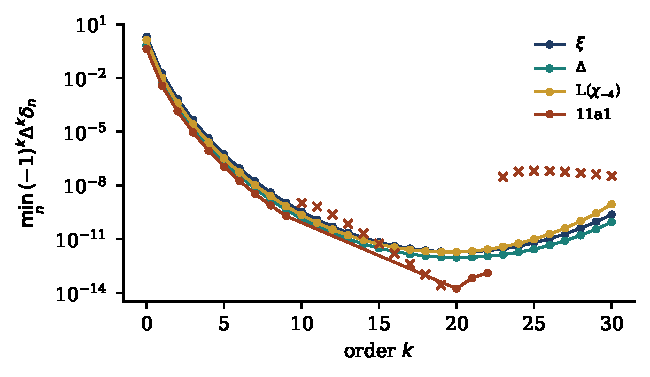
\includegraphics[width=0.78\textwidth]{figs/patie_test.pdf}
\caption{$\min_n(-1)^k\Delta^k\delta_n$ against the order $k$ for $\xi$, $\Delta$, $L(s,\chi_{-4})$ (no violation through $k=30$) and 11a1 (crosses: absolute values of negative minima, from $k = 10$).}\label{fig:10dpatie}
\end{figure}

Figure~\ref{fig:10dpatieheat} shows the whole table rather than its minima: for $\xi$ every entry of $(-1)^k\Delta^k\delta_n$ is positive, while for 11a1 a negative region opens from order $k=10$.

\begin{figure}[ht]\centering
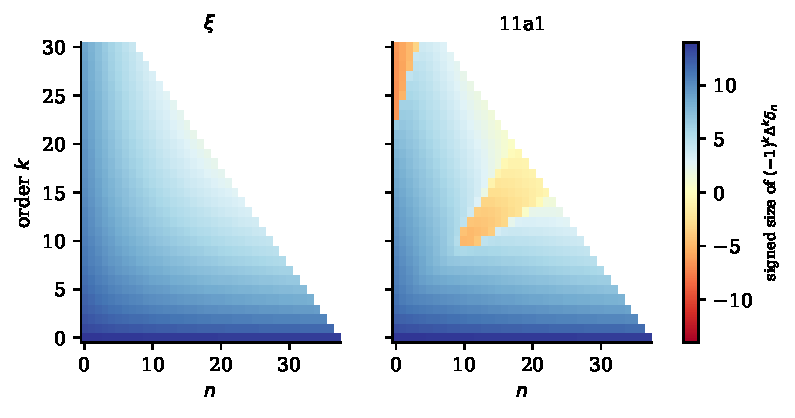
\includegraphics[width=0.95\textwidth]{figs/patie_heatmap.pdf}
\caption{Signed size of $(-1)^k\Delta^k\delta_n$ (blue positive, red negative, logarithmic scale) for $\xi$ and for the elliptic curve 11a1, computed from 40 central Taylor coefficients at 350 digits.}\label{fig:10dpatieheat}
\end{figure}

By Theorem~\ref{thm:10dpatie}, if $\Xi_\pi(it)/\Xi_\pi(0) = J_\Psi$, the partner would be $\sqrt2B_T$ with $T$ self decomposable and $\E e^{-sT} = \Xi_\pi(0)/\Xi_\pi(\sqrt s)$. Under GRH this is consistent with Theorem~\ref{thm:10dvdp}, where $V_\pi = \sqrt{2Z_\pi}N$ and $Z_\pi$, a GGC, is self decomposable; for $\xi$, self decomposability of $T$ is the unconditional statement of \cite{polson2018vdp} quoted above. Membership would add a structure on the Taylor coefficients, the factorisation $a_0/a_n = \Psi(1)\cdots\Psi(n)$ through a L\'evy exponent. A representing $\Psi$ would have no Brownian component. Indeed $\Psi(u)/u^2\to\sigma^2/2$ for any such exponent, and if $\Psi(n)\ge\epsilon n^2$ for all large $n$ then $a_n\le Ca_0\epsilon^{-n}(n!)^{-2}$, so $|\Xi_\pi(z)|\le C'e^{2|z|/\sqrt\epsilon}$, contradicting the growth $\exp(cx\log x)$ of $\Xi_\pi(x)$ on the real axis forced by the Gamma factors; hence $\liminf\Psi(n)/n^2 = 0$ and $\sigma = 0$. For $\xi$ the ratios $\Psi(n)/n^2$ are $43.3$, $23.3$, $16.5$, $13.0$, $10.9$ for $n = 1,\dots,5$. Interpolating the $\Psi(n)$ by a Bernstein gamma type function is a well posed computational problem (Computational Problem~\ref{cp:10dpatie}).

\section{Notes}

The van Dantzig problem was posed in 1958 \cite{vandantzig1958}; Lukacs \cite{lukacs1968,lukacs1970} introduced the class we call $\mathcal D_L$ and the operators $L^{(p)}$, and Ostrovskii \cite{ostrovskii1970} constructed hyperbolic examples. Hinds \cite{hinds1974} studied the Gamma and symmetric Beta examples; for the latter see also \cite{amdeberhan2012,jurek2010,hasebesimonwang2018}, and for Bessel hitting times Kent \cite{kent1978}. Thorin \cite{thorin1977} introduced generalized gamma convolutions and Bondesson \cite{bondesson1992} developed them, including the extended class. Biane, Pitman and Yor \cite{bpy2001} gave the Brownian reading of $\xi$, and Biane \cite{biane2009} the matrix Brownian reading of P\'olya's Macdonald function theorem \cite{polya1926}. Wald couples with infinitely divisible members are due to Roynette and Yor \cite{roynetteyor2005}, building on Hartman's theorem on the reciprocal Gamma function \cite{hartman1976}; they also rewrote the Riemann hypothesis through Wald couples and P\'olya frequency functions (their Th\'eor\`eme~V.3.2) and observed that the P\'olya variable of $\xi$ is not infinitely divisible. The equivalence between Hadamard factorisation, van Dantzig pairs, Wald couples and Thorin's condition, the $2\sin^2$ lemma, the transport of Euler product L\'evy measures, and the shifted Thorin representations of $\xi$ are from the first author \cite{polson2017,polson2018vdp}. Konstantopoulos, Patie and Sarkar \cite{konstantopoulospatiesarkar2024} proved the Lukacs class characterisation of the Riemann hypothesis and of the Lee Yang property \cite{leeyang1952,newman1974,newmanwu2020}, and introduced $\mathcal D_P$ through the Bernstein gamma functions of Patie and Savov \cite{patiesavov2018}. The positivity criterion for $\xi$ is due to Hinkkanen \cite{hinkkanen1997} and Lagarias \cite{lagarias1999}; Weil's explicit formula \cite{weil1952} is used in the form of \cite{iwanieckowalski2004}. Kendall's identity is from \cite{kendall1957}, the ballot theorem from Tak\'acs \cite{takacs1967}, and fluctuation theory of spectrally negative processes from \cite{bertoin1996,kyprianou2014}. Ours are Theorem~\ref{thm:10dvdp} and Theorem~\ref{thm:10dshift} in the generality of Chapter~\ref{ch:10b} (for $\zeta$ they are due to the authors cited above), Proposition~\ref{prop:10dsmooth}, the Thorin density $u_\Gamma$ in \eqref{eq:10dnewman}, Proposition~\ref{prop:10dsublaw}, Theorem~\ref{thm:10dballot}, Proposition~\ref{prop:10dpatietest} and all computations; each is an elementary consequence of the cited results, and none proves a Riemann hypothesis.

\section{Exercises}

\begin{enumerate}
\item Verify that $\frac2{\sqrt\pi}e^{x-e^{2x}}$ is a probability density with characteristic function $\frac1{\sqrt\pi}\Gamma(\frac{1+is}2)$, and prove $|\Gamma(\frac{1+is}2)|^2 = \pi/\cosh(\pi s/2)$. Show that $t\mapsto\sqrt\pi/\Gamma(\frac{1-t}2)$ takes the values $-\frac12$ at $t=2$ and $2$ at $t=-2$, so that it is neither even nor bounded by $1$; deduce that the Hinds law is not in $\mathcal D$, while the product is.
\item\label{ex:10dbeta} For $\nu>-\frac12$ expand $\cos(sx)$ and use Beta integrals to show that the symmetric Beta law of density $(1-x^2)^{\nu-1/2}/B(\nu+\frac12,\frac12)$ has characteristic function $\Gamma(\nu+1)(s/2)^{-\nu}J_\nu(s)$. Identify the cases $\nu = 0,\frac12,1$, and the limit $\nu\downarrow-\frac12$.
\item Prove the Laplace pair $\int_0^\infty e^{-yz}\cos(2\sqrt{az})(\pi z)^{-1/2}dz = y^{-1/2}e^{-a/y}$ and deduce \eqref{eq:10dpair}. Then, for $f(w) = w^2+\gamma^2$ at $\alpha = \epsilon$, where $\nu$ is a signed measure, check directly that the two expressions in \eqref{eq:10dU} agree, recovering the single zero case of Proposition~\ref{prop:10dsmooth}.
\item Show that $d_1 = 1$ and that $d_2$ is the divisor function. For $\sigma>1$ and $t>0$ compute $\E X_t$ and $\operatorname{Var}X_t$ in terms of $\zeta'/\zeta$ and its derivative, and check the first entry $\Prob(M_1 = 1) = \zeta(2)^{-1/2}\cdot1 = 0.77970$ of the table for $\sigma = 2$, $c = \frac12$.
\item\label{ex:10dnotid} Show that the characteristic function of an infinitely divisible law has no real zero. (If $\varphi = \varphi_n^n$ for every $n$, then $|\varphi_n|^2 = |\varphi|^{2/n}$ converges to the indicator of $\{\varphi\ne0\}$, which is therefore continuous at $0$ and a characteristic function, hence identically $1$.) Deduce that $W_\zeta$ and $W_\Delta$ are not infinitely divisible (Remark~\ref{rem:10dnotid}).
\item For $\cos t$ show that the Patie test of Proposition~\ref{prop:10dpatietest} gives $\Psi(n) = 2n(2n-1)$, the exponent $\Psi(u) = 4u^2-2u$ of Brownian motion with variance $8$ and drift $-2$, with largest zero $\frac12$, and that $\delta_n = 8$. Do the same for $\sin t/t$ and for $f_\nu$ of \eqref{eq:10dbeta}, and compare with Theorem~\ref{thm:10dpatie}.
\end{enumerate}

\section{Open computational problems}

\begin{compproblem}[Certified Patie test and Bernstein gamma interpolation]\label{cp:10dpatie}
Objective: certify the Hausdorff inequalities of Proposition~\ref{prop:10dpatietest} for $\xi$, $\Delta$ and $L(s,\chi_{-4})$ through order $k = 100$, and attempt to reconstruct $\Psi$. Objects and scale: the first $120$ central Taylor coefficients of each completed function. Route: coefficients in rigorous ball arithmetic (Arb, cross checked with PARI/GP \texttt{lfunlambda} at $2000$ digits), interval finite differences, then a least squares fit of $\Psi(u) = au+\int(e^{-ur}-1+ur\mathrm{1}_{\{r<1\}})\Pi(dr)$ with $\Pi$ a positive combination of $r^{-1-\beta}e^{-\lambda r}$, via the Bernstein gamma recursion of \cite{patiesavov2018}. Deliverable: certified lower bounds for $\min_n(-1)^k\Delta^k\delta_n$, the first certified violation if any, and the fitted L\'evy measure with residuals. Why it matters: a certified violation answers the question of Konstantopoulos, Patie and Sarkar negatively for $\xi$; a stable fit suggests a candidate Brownian subordination structure for the partner of $\xi$.
\end{compproblem}

\begin{compproblem}[Transported Thorin densities in the strip]
Objective: map the sign of the total transported density $V_a$ of Theorem~\ref{thm:10dshift}, and of its arithmetic and archimedean parts, for basepoints $\alpha = \frac12+a\in(\frac12,1]$. Objects and scale: $\xi$, $\Delta$ and $L(s,\chi_{-4})$, $a\in\{0.01,0.02,\dots,0.5\}$, $\sqrt z\le10^4$; the arithmetic part from all primes below $10^9$ with smoothing. Route: PARI/GP \texttt{lfunlambda} derivatives on GPU grids; interval arithmetic near the minima. Deliverable: the region of the $(a,z)$ plane where positivity is certified, the minimum of $V_a$ for each $a$, the location of the minima relative to the $\gamma_k^2$, and, for $\Lambda(s,\chi_{-4})$, the margin $\min_{t\ge1}\bigl(\operatorname{Re}\Lambda'/\Lambda(\alpha+it)-\Lambda'/\Lambda(\alpha)\bigr)$ in Theorem~\ref{beta:thm:minall}. Why it matters: by the argument of Theorem~\ref{thm:10dshift}(iv), certified positivity of $V_{a'}$ on $\sqrt z\le T$ for every $a'\ge a$ (interval arithmetic in $a'$ as well as in $z$) excludes zeros with real part above $\frac12+a$ and height at most $T$, so the map is a Thorin form of zero free region computations.
\end{compproblem}

\begin{compproblem}[First passage tables and large deviations for Euler subordinators]
Objective: tabulate the first passage laws of Theorem~\ref{thm:10dballot} and their large deviations. Objects and scale: $\zeta$, $\zeta_K$ for the $100$ quadratic and cubic fields of smallest discriminant, and the Rankin Selberg functions $L(s,\pi\times\tilde\pi)$, partial or complete, for the eleven functions of Table~\ref{tab:10bcatalogue}; $\sigma\in\{1.1,1.5,2\}$, $x\le50$, $m\le10^8$. Route: generalized divisor functions by sieving, $\Phi$ by Newton iteration on $\psi$, Monte Carlo with $10^7$ paths. Deliverable: tables of $\Prob(M_x = m)$, verification of $\sum_m\Prob(M_x=m) = 1$ to $10^{-10}$, and the rate function $\lim x^{-1}\log\Prob(\tau_x>\theta x)$ compared with the Legendre transform of $\psi$. Why it matters: these are the probabilistic objects attached to $\pi$ to the right of $1$, and their behaviour as $\sigma\downarrow1$ is governed by the pole and the zero free region of $L(s,\pi\times\tilde\pi)$.
\end{compproblem}

\begin{compproblem}[Van Dantzig and P\'olya frequency tests across LMFDB]
Objective: test numerically, without zeros, whether the partner $\Xi_\pi(0)/\Xi_\pi(t)$ is the characteristic function of a P\'olya frequency density. Objects and scale: all self dual $L$ functions in LMFDB of degree at most $4$ and conductor below $10^4$, whether or not the P\'olya kernel is positive. Route: evaluate $\Xi_\pi(t)$ on $|t|\le200$ with PARI/GP, invert the Fourier transform by quadrature with error control, and compute Toeplitz determinants $\det[g(x_i-y_j)]$ of orders $2$ to $6$ on random grids. Deliverable: for each function the minimum density, the smallest Toeplitz minor found, and a table of failures with diagnosis (quadrature error or genuine). Why it matters: by Theorem~\ref{thm:10dvdp} the P\'olya frequency property of $V_\pi$ is equivalent to GRH, and log concavity, observed here for $\Delta$, is its first rung.
\end{compproblem}

\chapter[Squarefree Integers and Thorin Atoms]{Squarefree Integers and the Thorin Atoms of $\Xi$}\label{ch:squarefree}

The squarefree integers\index{squarefree integers} are a simple arithmetic sequence whose fine structure is controlled by the zeros of $\zeta$, through the doubled argument $2s$. Their generating function is
\[
D(s)=\sum_{n\ge1}\frac{\mu(n)^2}{n^s}=\frac{\zeta(s)}{\zeta(2s)},
\]
so every nontrivial zero $\rho$ of $\zeta$ becomes a pole of $D$ at $\rho/2$ (unless $\zeta(\rho/2)=0$, which RH excludes), and the critical line $\operatorname{Re} s=\frac12$ is carried to $\operatorname{Re} s=\frac14$. This chapter reads that picture through two objects of Chapters~\ref{ch:10} and~\ref{ch:10b}: the P\'olya density of $\Xi$ and the Thorin measure of $1/\Xi$. Three things come out of it. Under RH the poles of $D$ in the strip $0<\operatorname{Re}s<\frac12$ correspond to the Thorin atoms $\gamma_k^2$ through $\gamma_k^2=-(2s-\frac12)^2$; the constant $\kappa$ of the squarefree problem is a combination of two tilted means of the P\'olya law; and smoothing the squarefree count by a Gamma(2) law turns its error into a positive average of the Mertens function, with Gamma(2) the largest shape for which that holds. Section~\ref{sec:sf:computing} records how the numbers quoted are computed.

The starting point is a Math StackExchange question~\cite{mathstackexchange2016} on the asymptotics of $\sum_{n\le x}\mu(n)^2n^{-\alpha}$, especially at $\alpha=1$. Section~\ref{sec:sf:classical} answers it.

\section{The classical problem}\label{sec:sf:classical}

Let $Q(x)=\sum_{n\le x}\mu(n)^2$ and $\Delta(x)=Q(x)-6x/\pi^2$. From $\mu(n)^2=\sum_{d^2\mid n}\mu(d)$,
\begin{equation}\label{eq:sf:Qd}
Q(x)=\sum_{d\le\sqrt x}\mu(d)\Bigl\lfloor\frac{x}{d^2}\Bigr\rfloor=\frac{6}{\pi^2}x-\sum_{d\le\sqrt x}\mu(d)\Bigl\{\frac{x}{d^2}\Bigr\}+O(\sqrt x),
\end{equation}
so $\Delta(x)=O(\sqrt x)$. The terms $\mu(d)\{x/d^2\}$ will return in Section~\ref{sec:sf:gamma2}.

\subsection{Perron's formula over a number field}
For a number field $K$ with Dedekind zeta function $\zeta_K$, the ideal analogue of $D$ has Euler factor $1+N(\mathfrak{p})^{-s}=(1-N(\mathfrak{p})^{-2s})/(1-N(\mathfrak{p})^{-s})$, hence equals $\zeta_K(s)/\zeta_K(2s)$, and Perron's formula\index{Perron's formula} gives
\begin{equation}\label{eq:sf:perron}
Q_\alpha(x)=\sum_{N(\mathfrak{a})\le x}\frac{\mu^2(\mathfrak{a})}{N(\mathfrak{a})^\alpha}=\frac{1}{2\pi i}\int_{(c)}\frac{\zeta_K(s+\alpha)}{\zeta_K(2s+2\alpha)}\,x^s\,\frac{ds}{s},\qquad c>\max(0,1-\alpha),
\end{equation}
for $x$ not the norm of an ideal. The integrand has a simple pole at $s=1-\alpha$, a simple pole at $s=0$, and poles at $s=\rho/2-\alpha$ for the zeros $\rho$ of $\zeta_K$ with $\zeta_K(\rho/2)\ne0$. Let $c_K=\operatorname{Res}_{s=1}\zeta_K(s)$, and define the Euler Kronecker constant\index{Euler Kronecker constant} $\gamma_K$~\cite{ihara2006} by $\zeta_K(s)=c_K/(s-1)+c_K\gamma_K+O(s-1)$.

\begin{proposition}\label{prop:sf:classical}
For $\alpha=1$ the poles at $s=1-\alpha$ and $s=0$ merge into a double pole at $s=0$, and
\begin{equation}\label{eq:sf:alpha1K}
\sum_{N(\mathfrak{a})\le x}\frac{\mu^2(\mathfrak{a})}{N(\mathfrak{a})}=\frac{c_K}{\zeta_K(2)}\bigl(\log x+\kappa_K\bigr)+o(1),\qquad \kappa_K=\gamma_K-\frac{2\zeta_K'(2)}{\zeta_K(2)} .
\end{equation}
Over $\Q$, with $A$ the Glaisher Kinkelin constant\index{Glaisher Kinkelin constant},
\begin{equation}\label{eq:sf:final}
\sum_{n\le x}\frac{\mu(n)^2}{n}=\frac{6}{\pi^2}\bigl(\log x+\kappa\bigr)+O\bigl(x^{-1/2}\bigr),
\end{equation}
where $\kappa=24\log A-\gamma_{\mathrm E}-2\log2\pi=1.7171376511\ldots$, and for real $\alpha>\frac12$ with $\alpha\ne1$ the residues at $s=1-\alpha$ and $s=0$ give
\[
\sum_{n\le x}\frac{\mu(n)^2}{n^\alpha}=\frac{6}{\pi^2}\,\frac{x^{1-\alpha}}{1-\alpha}+\frac{\zeta(\alpha)}{\zeta(2\alpha)}+O\bigl(x^{\frac12-\alpha}\bigr).
\]
\end{proposition}

\begin{proof}
Let $Q_1(x)$, as in~\eqref{eq:sf:perron}, be the left side of~\eqref{eq:sf:alpha1K}. Summation by parts from the count of squarefree ideals, $\frac{c_K}{\zeta_K(2)}x+O(x^\theta)$ with some $\theta<1$ (from $\mu^2(\mathfrak a)=\sum_{\mathfrak d^2\mid\mathfrak a}\mu(\mathfrak d)$ and the ideal count $c_Ky+O(y^{1-1/[K:\Q]})$), gives $Q_1(x)=\frac{c_K}{\zeta_K(2)}\log x+C+O(x^{\theta-1})$. As $s\downarrow0$, $s\int_1^\infty Q_1(t)t^{-s-1}dt=\zeta_K(1+s)/\zeta_K(2+2s)$ is therefore $\frac{c_K}{\zeta_K(2)}\frac1s+C+o(1)$, and it is also $\frac{c_K}{\zeta_K(2)}(\frac1s+\kappa_K)+O(s)$, because $\kappa_K$ is the logarithmic derivative of $(s-1)\zeta_K(s)/\zeta_K(2s)$ at $s=1$. So $C=\frac{c_K}{\zeta_K(2)}\kappa_K$, and the main term is the residue at the double pole. Over $\Q$ use $\gamma_{\Q}=\gamma_{\mathrm E}$ and $\zeta'(2)/\zeta(2)=\gamma_{\mathrm E}+\log2\pi-12\log A$. For the error term, write $B(x)=\sum_{n\le x}(\mu(n)^2-6/\pi^2)=\Delta(x)+O(1)=O(\sqrt x)$ and sum by parts: the tail $\int_x^\infty B(t)t^{-2}dt$ and the boundary term $B(x)/x$ are both $O(x^{-1/2})$. For $\alpha\ne1$ the same summation by parts gives the error $O(x^{\frac12-\alpha})$ and a constant which, as a function of $\alpha$, is meromorphic in $\operatorname{Re}\alpha>\frac12$ and equals $\zeta(\alpha)/\zeta(2\alpha)$ for $\alpha>1$, hence for all $\alpha>\frac12$.
\end{proof}

The answers in~\cite{mathstackexchange2016} give the $\log x$ term and, for $\alpha\ne1$, the first main term; the second answer reaches~\eqref{eq:sf:final} with error $o(1)$ and the constant left as $\sum_n(\mu(n)^2-6/\pi^2)/n$, which equals $-2\zeta'(2)/\zeta(2)^2$. For $\frac12<\alpha<1$ the constant $\zeta(\alpha)/\zeta(2\alpha)$ is negative, for example $\zeta(\frac34)/\zeta(\frac32)=-1.3173\ldots$; Corollary~\ref{cor:sf:sign} reads the sign through the P\'olya density.

\section{The P\'olya density}\label{sec:sf:polya}

Let $\xi$, $\Xi$ and P\'olya's kernel $\Phi$ be as in~\eqref{eq:ch10polya}\index{P\'olya kernel}, so that $\xi(\frac12+z)=\int_{\R}\Phi(u)e^{zu}\,du$ for all complex $z$, and let $W_\zeta$, with density $\Phi/\Xi(0)$, be the P\'olya variable of $\zeta$ (Lemma~\ref{lem:10bkernel} and the paragraph after it). Put $T=W_\zeta/2$, whose density is $p(t)=2\Phi(2t)/\Xi(0)$, and $M_T(\theta)=\E[e^{\theta T}]$. Then
\begin{equation}\label{eq:sf:xiM}
\xi\bigl(\tfrac12+w\bigr)=\xi\bigl(\tfrac12\bigr)\,M_T(2w),\qquad \xi\bigl(\tfrac12\bigr)=0.4971207781\ldots
\end{equation}
Applying the definition of $\xi$ at $s$ and $2s$, and the duplication formula for $\Gamma(s)$, gives the following.

\begin{proposition}\label{prop:sf:polya}
For all $s$,
\[
\frac{\zeta(s)}{\zeta(2s)}=\omega(s)\,\frac{M_T(2s-1)}{M_T(4s-1)},\qquad \omega(s)=\frac{2s-1}{s-1}\,2^{s}\,\pi^{-(s+1)/2}\,\Gamma\Bigl(\frac{s+1}{2}\Bigr).
\]
\end{proposition}

The factor $1/(s-1)$ carries the pole at $s=1$, and $2s-1$ gives the zero of $D$ at $s=\frac12$, where $\zeta(2s)$ has its pole. In $\operatorname{Re}s>-1$ every other singularity of $D$ is a zero of $M_T(4s-1)$; the poles of $\Gamma(\frac{s+1}2)$ give the poles of $D$ at $s=-1,-3,\dots$.

\begin{corollary}[sign of the constant]\label{cor:sf:sign}
For real $\alpha>-1$ with $\alpha\ne\frac12,1$, the sign of $\zeta(\alpha)/\zeta(2\alpha)$ is the sign of $(2\alpha-1)/(\alpha-1)$. In particular it is negative exactly on $\frac12<\alpha<1$.
\end{corollary}

\begin{proof}
$M_T>0$ on the real line, and the gamma factor in $\omega$ is positive for $\alpha>-1$. Directly, $\zeta<0$ on $(-2,1)$ and $\zeta>0$ on $(1,\infty)$.
\end{proof}

At $\alpha=\frac34$, for instance,
\[
\omega\bigl(\tfrac34\bigr)=-1.3461\ldots,\qquad \frac{M_T(\frac12)}{M_T(2)}=\frac{\xi(\frac34)}{\xi(\frac32)}=0.9786\ldots,
\]
and their product is $\zeta(\frac34)/\zeta(\frac32)=-1.3173\ldots$.

\subsection{The constant as tilted P\'olya means}
Let $\E_\theta$ denote expectation under the tilted law $e^{\theta t}p(t)/M_T(\theta)$, so that $\E_\theta[T]=(\log M_T)'(\theta)$. Index the zeros of $\xi$ as $\rho=\frac12+i\gamma_\rho$ and let $\sum_\rho$ run over those with $\operatorname{Re}\gamma_\rho>0$, with multiplicity. By Hadamard's product and~\eqref{eq:sf:xiM},
\begin{equation}\label{eq:sf:logM}
\log M_T(\theta)=\sum_\rho\log\Bigl(1+\frac{\theta^2}{4\gamma_\rho^2}\Bigr),\qquad \E_\theta[T]=\sum_\rho\frac{2\theta}{\theta^2+4\gamma_\rho^2}.
\end{equation}

\begin{theorem}\label{thm:sf:const}
The constant in~\eqref{eq:sf:final} is
\[
\begin{aligned}
\kappa&=2+\log2-\tfrac12\log\pi-\tfrac12\gamma_{\mathrm E}+2\,\E_1[T]-4\,\E_3[T]\\
&=2+\log2-\tfrac12\log\pi-\tfrac12\gamma_{\mathrm E}+\sum_\rho\Bigl(\frac{4}{1+4\gamma_\rho^2}-\frac{24}{9+4\gamma_\rho^2}\Bigr).
\end{aligned}
\]
\end{theorem}

\begin{proof}
$\kappa$ is the logarithmic derivative of $(s-1)D(s)$ at $s=1$. Take logarithms in Proposition~\ref{prop:sf:polya}, differentiate at $s=1$, use $\psi(1)=-\gamma_{\mathrm E}$, and apply~\eqref{eq:sf:logM}.
\end{proof}

Numerically $\E_1[T]=0.0115478545$ and $\E_3[T]=0.0345331158$, and the theorem reproduces $\kappa$ to twenty digits. The first sixty zeros contribute $-0.0944$ of the zero sum $-0.1150$, the tail being about $-5\sum_{k>60}\gamma_k^{-2}$. Thus the arithmetic content of the constant is two tilted means of the P\'olya law, at the tilts $1=2s-1$ and $3=4s-1$ evaluated at $s=1$.

Comparing coefficients of $\theta^{2m}$ in~\eqref{eq:sf:logM} gives the cumulants of $W_\zeta=2T$, as in Proposition~\ref{prop:10bcumulants}:
\begin{equation}\label{eq:sf:cumulants}
\kappa_{2m}(2T)=(-1)^{m+1}\frac{(2m)!}{m}S_m,\qquad S_m=\sum_\rho\gamma_\rho^{-2m},
\end{equation}
and in particular $S_1=2\operatorname{Var}(T)=0.0231049931\ldots$ These identities are unconditional. Under RH the even cumulants of $T$ alternate in sign.

\section{Thorin atoms are the poles in the strip}\label{sec:sf:thorin}

Generalized gamma convolutions (GGC) and their Thorin measures are as in Definition~\ref{def:ch10ggc}; their Laplace transforms continue analytically and without zeros to $\C\setminus(-\infty,0]$ (Lemma~\ref{lem:ch10nonvanish}).

\begin{proposition}[Theorem~\ref{thm:10bmain} for $\zeta$; after \cite{polson2017}]\label{prop:sf:thorin}
RH holds if and only if the function $u\mapsto\xi(\frac12)/\xi(\frac12+\sqrt u)$ is a GGC Laplace transform. Then
\[
\frac{\xi(\frac12)}{\xi(\frac12+\sqrt u)}=\prod_{k\ge1}\Bigl(1+\frac{u}{\gamma_k^2}\Bigr)^{-1}=\E\bigl[e^{-uY}\bigr],\qquad Y=\sum_{k\ge1}\frac{E_k}{\gamma_k^2},
\]
with $E_k$ independent standard exponential variables, drift $0$ and Thorin measure $\tau=\sum_k\delta_{\gamma_k^2}$. Moreover $\E[Y]=2\operatorname{Var}(T)$.
\end{proposition}

\begin{proof}
This is Theorem~\ref{thm:10babstract} for $E(z)=\xi(\frac12+z)/\xi(\frac12)$, the function $\Xi_\zeta$ of Definition~\ref{def:10bxi} normalised at $0$; the mean is $S_1$, by~\eqref{eq:sf:cumulants}.
\end{proof}

Theorem~\ref{thm:10babstract} applies equally to Dedekind zeta functions (Definition~\ref{def:10bxi}). Let $\xi_K(s)=s(s-1)|d_K|^{s/2}\Gamma_{\R}(s)^{r_1}\Gamma_{\C}(s)^{r_2}\zeta_K(s)$, with $\Gamma_{\R}(s)=\pi^{-s/2}\Gamma(\frac s2)$ and $\Gamma_{\C}(s)=2(2\pi)^{-s}\Gamma(s)$.

\begin{proposition}[Theorem~\ref{thm:10babstract} for $\zeta_K$]\label{prop:sf:thorinK}
If $\zeta_K(\frac12)\ne0$, then $\xi_K(\frac12)/\xi_K(\frac12+\sqrt u)$ is a GGC Laplace transform if and only if the Riemann hypothesis holds for $\zeta_K$, and its Thorin measure is then $\sum_k\delta_{\gamma_k^2}$ over the positive ordinates of the zeros of $\zeta_K$.
\end{proposition}

A real zero $\frac12+x$ with $x>0$, a Siegel zero in particular, gives a pole at $u=x^2>0$, as in the proof of Theorem~\ref{thm:ch10general}. The hypothesis $\zeta_K(\frac12)\ne0$ fixes the normalisation: Armitage~\cite{armitage1972} exhibited a number field, from a construction of Serre, where it fails, and there one divides by $u^m$, where $2m$ is the order of the zero at $\frac12$, as in Definition~\ref{def:10bxi}.

\subsection{The recentred series}
Put $s=\frac14+\frac12\sqrt u$, so that $2s=\frac12+\sqrt u$. By Proposition~\ref{prop:sf:polya} and~\eqref{eq:sf:xiM},
\[
D\bigl(\tfrac14+\tfrac12\sqrt u\bigr)=\omega\bigl(\tfrac14+\tfrac12\sqrt u\bigr)\,\xi\bigl(\tfrac14+\tfrac12\sqrt u\bigr)\,\frac{1}{\xi(\frac12+\sqrt u)},
\]
and under RH the last factor is $\xi(\frac12)^{-1}\E[e^{-uY}]$. The atom $\gamma_k^2$ of the Thorin measure gives the pole at $u=-\gamma_k^2$, that is at $s=\frac14\pm\frac i2\gamma_k=\rho_k/2$.\index{Thorin atom} Under RH the poles of the squarefree series in $0<\operatorname{Re} s<\frac12$ are therefore exactly the Thorin atoms of $1/\Xi$, and the same holds over $K$ under the Riemann hypothesis for $\zeta_K$ by Proposition~\ref{prop:sf:thorinK}, with an extra pole at $s=\frac14$ when $\zeta_K(\frac12)=0$.

\subsection{What each atom contributes}
At a simple zero, the Perron residue of $D(s)x^s/s$ at $\rho/2$ is $R_\rho\,x^{\rho/2}$ with
\begin{equation}\label{eq:sf:Rrho}
R_\rho=\frac{\zeta(\rho/2)}{\rho\,\zeta'(\rho)},\qquad R_{\rho_1}=0.02880-0.09618\,i,\quad |R_{\rho_1}|=0.10040\ldots
\end{equation}
Formally\index{explicit formula} $\Delta(x)\approx1+2\operatorname{Re}\sum_kR_{\rho_k}x^{\rho_k/2}$, where $1$ is the residue at $s=0$. Under RH every term has size $x^{1/4}$. Figure~\ref{fig:sf:atoms} compares sixty atoms with the exact error.

\begin{figure}[t]
\centering
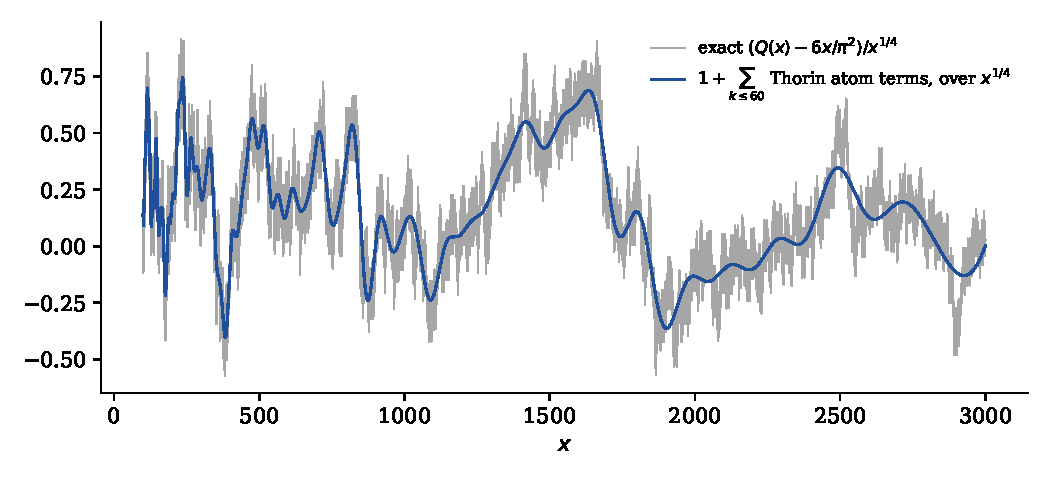
\includegraphics[width=\textwidth]{figs/sf_atoms.pdf}
\caption{The normalised error $\Delta(x)/x^{1/4}$ on $[100,3000]$ (grey) and the contribution of the first sixty Thorin atoms, $\bigl(1+2\operatorname{Re}\sum_{k\le60}R_{\rho_k}x^{\rho_k/2}\bigr)/x^{1/4}$ (blue). Correlation about $0.92$.}
\label{fig:sf:atoms}
\end{figure}

The atom series is not known to converge, even on RH: the Perron weight $1/s$ decays only like $1/|\gamma|$, and nothing controls the sizes of $\zeta(\rho/2)$ and $1/\zeta'(\rho)$ well enough. On RH, Montgomery and Vaughan~\cite{montgomeryvaughan1981} proved $\Delta(x)\ll x^{1/3+\varepsilon}$ and Liu~\cite{liu2016} $\Delta(x)\ll x^{11/35+\varepsilon}$; the conjectured bound $\Delta(x)\ll x^{1/4+\varepsilon}$ remains open on RH~\cite{mot2021,gmrr2021} (Open Problem~\ref{op:sfquarter}).

\section{Smoothed, averaged and extreme values}\label{sec:sf:smooth}

\subsection{Exponential smoothing}
Let $S(x)=\sum_n\mu(n)^2e^{-n/x}=\frac{1}{2\pi i}\int_{(2)}\Gamma(s)D(s)x^s\,ds$.

\begin{theorem}\label{thm:sf:smooth}
RH holds if and only if $S(x)=6x/\pi^2+O_\varepsilon(x^{1/4+\varepsilon})$ for every $\varepsilon>0$. Under RH with simple zeros, and with the zeros summed over $\gamma_k<T_\nu$ for a suitable sequence $T_\nu\to\infty$~\cite[Ch.~14]{titchmarsh1986},
\[
S(x)=\frac{6}{\pi^2}x+1+2\operatorname{Re}\sum_k\frac{\Gamma(\rho_k/2)\,\zeta(\rho_k/2)}{2\,\zeta'(\rho_k)}\,x^{\rho_k/2}-\frac{\zeta(-1)}{2\zeta'(-2)}\,\frac{\log x}{x}+O\Bigl(\frac1x\Bigr).
\]
\end{theorem}

\begin{proof}
Assume RH. Then $1/\zeta(\sigma+it)\ll|t|^\varepsilon$ for $\sigma\ge\frac12+\varepsilon$~\cite[Thm.~14.2]{titchmarsh1986}, $\zeta$ grows polynomially on vertical lines and $\Gamma$ decays exponentially, so the line of integration moves to $\operatorname{Re} s=\frac14+\varepsilon$, crossing only the pole at $s=1$. Moving further left collects the atoms at $\rho/2$, the residue $1$ at $s=0$, and the double pole at $s=-1$, where $\Gamma$ has a pole and $\zeta(2s)$ a trivial zero.

Conversely, the Mellin transform of $S(1/y)-6/(\pi^2y)$ on $(0,1)$ plus that of $S(1/y)$ on $(1,\infty)$ equals $\Gamma(s)D(s)-6/(\pi^2(s-1))$, and the hypothesis makes it analytic in $\operatorname{Re} s>\frac14$. Since $\Gamma$ has no zeros, $D$ is analytic there except at $s=1$. Suppose $\zeta(\rho)=0$ with $\beta=\operatorname{Re}\rho>\frac12$. Then $\rho/2$ lies in $\operatorname{Re} s>\frac14$, so its pole must cancel: $\zeta(\rho/2)=0$. By the functional equation, $\rho'=1-\overline{\rho}/2$ is a zero with $\operatorname{Re}\rho'=1-\beta/2>\frac12$ and $\operatorname{Im}\rho'=\operatorname{Im}\rho/2$. Iterating produces distinct zeros accumulating at $\frac23$, the fixed point of $\beta\mapsto1-\beta/2$; they are distinct because $\zeta$ has no real zeros in $(0,1)$. This is impossible for a function analytic and not identically zero at $\frac23$. This descent is due to Keith Conrad; Mossinghoff, Oliveira e Silva and Trudgian~\cite{mot2021} give it for the sharp count.
\end{proof}

Table~\ref{tab:sf:smooth} checks the expansion at four values of $x$.

\begin{table}[t]
\centering
\begin{tabular}{rccc}
\toprule
$x$ & $S(x)-6x/\pi^2-1$ & forty atoms & $-\frac{\zeta(-1)}{2\zeta'(-2)}\frac{\log x}{x}$\\
\midrule
$10^3$ & $-9.711\times10^{-3}$ & $\phantom{-}8.2\times10^{-5}$ & $-9.45\times10^{-3}$\\
$10^4$ & $-1.577\times10^{-3}$ & $-2.83\times10^{-4}$ & $-1.26\times10^{-3}$\\
$3\cdot10^4$ & $-7.41\times10^{-4}$ & $-2.59\times10^{-4}$ & $-4.70\times10^{-4}$\\
$10^5$ & $\phantom{-}4.23\times10^{-4}$ & $\phantom{-}5.83\times10^{-4}$ & $-1.58\times10^{-4}$\\
\bottomrule
\end{tabular}
\caption{Theorem~\ref{thm:sf:smooth}. The left column equals the sum of the other two to within $4\times10^{-5}$ for $x\ge10^4$; at $x=10^3$ the difference, $-3.4\times10^{-4}$, is the $O(1/x)$ term $-0.339/x$ of the theorem. The atoms are damped by $\Gamma(\rho/2)$, of size $e^{-\pi\gamma/4}$.}
\label{tab:sf:smooth}
\end{table}

\subsection{Mean square and extreme values}

\begin{theorem}\label{thm:sf:meansq}
RH holds if and only if $\int_X^{2X}\Delta(x)^2\,dx\ll_\varepsilon X^{3/2+\varepsilon}$ for every $\varepsilon>0$.
\end{theorem}

\begin{proof}
Let $F(s)=\int_1^\infty\Delta(x)x^{-s-1}dx=D(s)/s-6/(\pi^2(s-1))$. Under RH, $F$ is analytic in $\operatorname{Re} s>\frac14$, and the Lindel\"of bounds $\zeta(\sigma+it)\ll|t|^{1/4+\varepsilon}$ and $1/\zeta(2\sigma+2it)\ll|t|^\varepsilon$ for $\sigma\ge\frac14+\varepsilon$ give $|F(\sigma+it)|\ll|t|^{-3/4+2\varepsilon}$. The bound is uniform in $\sigma\ge c=\frac14+\varepsilon$, and $F$ is bounded near $s=1$, so $\sup_{\sigma>c}\int_{\R}|F(\sigma+it)|^2\,dt<\infty$. Since $F(s)=\int_0^\infty\Delta(e^v)e^{-sv}\,dv$ for $\operatorname{Re}s>\frac12$, the Paley Wiener theorem for the half plane $\operatorname{Re}s>c$ gives $\int_0^\infty\Delta(e^v)^2e^{-2cv}\,dv<\infty$, that is $\int_1^\infty\Delta(x)^2x^{-2c-1}dx<\infty$, and hence $\int_X^{2X}\Delta^2\ll X^{3/2+2\varepsilon}$. Conversely, Cauchy Schwarz turns the hypothesis into absolute convergence of the integral for $F$ in $\operatorname{Re} s>\frac14$, and the descent in the proof of Theorem~\ref{thm:sf:smooth} gives RH.
\end{proof}

\begin{corollary}[part (ii) after Evelyn and Linfoot~\cite{evelynlinfoot1931} and Stark~\cite{stark1966}]\label{cor:sf:omega}
(i) Under RH, $|\Delta(x)|\le X^{1/4+\varepsilon}$ for all $x\in[X,2X]$ outside a set of measure $O(X^{1-\varepsilon})$.

(ii) Unconditionally, with $|R_{\rho_1}|=0.10040\ldots$ from~\eqref{eq:sf:Rrho},
\[
\limsup_{x\to\infty}\frac{\Delta(x)}{x^{1/4}}\ge|R_{\rho_1}|,\qquad\liminf_{x\to\infty}\frac{\Delta(x)}{x^{1/4}}\le-|R_{\rho_1}| .
\]
\end{corollary}

\begin{proof}
(i) is Chebyshev's inequality. For (ii) suppose $\Delta(x)\le c\,x^{1/4}$ for $x\ge x_0$, with $c<|R_{\rho_1}|$. The function $c\,x^{1/4}-\Delta(x)$ is eventually nonnegative and its Mellin transform $c/(s-\frac14)-F(s)$ has no real singularity in $(\frac14,\infty)$, since $\zeta(2s)$ has no real zeros there. By Landau's theorem (Lemma~\ref{lem:10clandau}, \cite{landau1905})\index{Landau's lemma} the transform converges in $\operatorname{Re} s>\frac14$, which already forces RH by the descent in the proof of Theorem~\ref{thm:sf:smooth}, and at $s=\sigma+\frac i2\gamma_1$
\[
\Bigl|\frac{c}{s-\frac14}-F(s)\Bigr|\le\frac{c}{\sigma-\frac14}-F(\sigma)+O(1)=\frac{c}{\sigma-\frac14}+O(1).
\]
As $\sigma\downarrow\frac14$ the left side is at least $|R_{\rho_1}|/(\sigma-\frac14)+O(1)$, since $F$ has a pole at $\rho_1/2$ with residue $R_{\rho_1}$ if $\rho_1$ is simple and a pole of higher order otherwise. Hence $|R_{\rho_1}|\le c$, a contradiction. The lower bound is symmetric.
\end{proof}

Part (ii) is Landau's oscillation argument applied to the first zero. Evelyn and Linfoot~\cite{evelynlinfoot1931} proved $\Delta(x)=\Omega(x^{1/4})$, and Stark~\cite{stark1966} gave the first effective constant, $2(1-\gamma_1/\gamma_2)|R_{\rho_1}|=0.0657\ldots$; Landau's argument gives the larger constant of (ii), but not effectively. Using many zeros, Mossinghoff, Oliveira e Silva and Trudgian~\cite{mot2021} prove $\limsup_{x\to\infty}\Delta(x)/x^{1/4}>3$ and $\liminf_{x\to\infty}\Delta(x)/x^{1/4}<-3$, and computing $Q(x)$ for all $x\le10^{18}$ they find $|\Delta(x)|<1.12543\,x^{1/4}$ there. Sieving to $2\times10^7$ and sampling at the integers gives root mean squares of $\Delta/X^{1/4}$ on $[X,2X]$ of $0.280$, $0.255$, $0.281$ and $0.353$ for $X=10^4,\ldots,10^7$, and maxima of $|\Delta|/X^{1/4}$ between $0.68$ and $0.98$.

\subsection{How much smoothing the sharp count needs}
Let $G_{n,x}$ have the Gamma($n$) law with mean $x$. It concentrates on a window of width $x/\sqrt n$, and $\E\,Q(G_{n,x})\to Q(x)$ as $n\to\infty$ when $x$ is not a squarefree integer.

\begin{proposition}\label{prop:sf:gamman}
Under RH, uniformly in $n\ge1$,
\[
\E\,Q(G_{n,x})=\frac{6}{\pi^2}x+O_\varepsilon\bigl(x^{1/4+\varepsilon}n^{1/8+\varepsilon}\bigr).
\]
\end{proposition}

\begin{proof}
With rate $\lambda=n/x$, $\E\,Q(G)=\frac1{2\pi i}\int D(s)\frac{\Gamma(s+n)}{s\,\Gamma(n)}(x/n)^s\,ds$. Shift to $\operatorname{Re} s=c=\frac14+\varepsilon$. From $|\Gamma(n+c+it)/\Gamma(n+c)|^{-2}=\prod_{k\ge0}(1+t^2/(n+c+k)^2)$, on that line
\[
\frac{|\Gamma(n+c+it)|}{\Gamma(n)}\ll n^c\exp\bigl(-c_0\min(t^2/n,|t|)\bigr)
\]
for an absolute $c_0>0$. With $|D(c+it)|\ll|t|^{1/4+\varepsilon}$ the integral is therefore
\[
\ll x^c\int(1+|t|)^{-3/4+\varepsilon}e^{-c_0\min(t^2/n,|t|)}\,dt\ll x^cn^{1/8+\varepsilon}.
\]
\end{proof}

At $n\asymp x^2$ the window has width $O(1)$ and the bound is the trivial $x^{1/2}$. The loss $n^{1/8}$ is the growth $|t|^{1/4}$ of $\zeta$ on $\operatorname{Re} s=\frac14$ integrated against $dt/|t|$ up to $|t|\asymp\sqrt n$. Removing it needs cancellation in $\int D(\frac14+it)x^{it}dt/t$, not a bound on its size.


\section{Gamma(2) smoothing and the Mertens function}\label{sec:sf:gamma2}

Return to the terms $\mu(d)\{x/d^2\}$ of \eqref{eq:sf:Qd}. Steutel and Thiemann \cite{steutelthiemann1989} studied when the integer and fractional parts of a random variable are independent, the exponential law being the basic case. We randomise $x$ by a Gamma(2) law and compute every term in closed form.

\subsection{Expected fractional parts}
Let $G$ have the Gamma(2) density $\lambda^2te^{-\lambda t}$ and $\theta=\lambda a$. Since $P(G\ge ma)=(1+m\theta)e^{-m\theta}$,
\begin{equation}\label{eq:sf:g}
\begin{aligned}
\E\lfloor G/a\rfloor&=\frac{1}{e^\theta-1}+\frac{\theta}{4\sinh^2(\theta/2)},\\
\E\{G/a\}=g(\theta)&=\frac2\theta-\frac{1}{e^\theta-1}-\frac{\theta}{4\sinh^2(\theta/2)} .
\end{aligned}
\end{equation}
With $\theta=2y$ the term $\theta/(4\sinh^2(\theta/2))$ equals $\theta^{-1}(y/\sinh y)^2$, and $(y/\sinh y)^2$ is the Laplace transform at $y^2/2$ of the sum of two independent hitting times of $1$ by a three dimensional Bessel process, through which Williams represents $\xi$ (Section~\ref{sec:ch10bpy}; \cite[Section~5]{williams1990} and \cite[(6) to (8) and Table~2]{bpy2001}). Expanding $1/(e^\theta-1)=\sum_me^{-m\theta}$ gives the Mellin transform $\int_0^\infty g(\theta)\theta^{s-1}d\theta=-(1+s)\Gamma(s)\zeta(s)$ for $0<\operatorname{Re} s<1$. Take $\lambda=2/X$, so that $\E G=X$, and write $G_X$. Summing \eqref{eq:sf:g} over $a=d^2$, now over all $d$ since $0\le g(\theta)\le\min(1,2/\theta)$,
\begin{equation}\label{eq:sf:EQ}
\E\,Q(G_X)=\sum_{n\ge1}\mu(n)^2\Bigl(1+\frac{2n}{X}\Bigr)e^{-2n/X}=\frac{6}{\pi^2}X-\sum_{d\ge1}\mu(d)\,g\Bigl(\frac{2d^2}{X}\Bigr).
\end{equation}
Table~\ref{tab:sf:EQ} checks this identity numerically.

\subsection{The Mertens representation}

\begin{theorem}\label{thm:sf:mertens}
The function
\[
f_V(v)=-2g'(v)=\frac{4}{v^2}-\frac{v\cosh(v/2)}{2\sinh^3(v/2)},\qquad v>0,
\]
is a probability density with $P(V\ge v)=2g(v)$ and $\E[V^s]=-2\Gamma(s+2)\zeta(s)$ for $0<\operatorname{Re} s<1$. With $M(t)=\sum_{d\le t}\mu(d)$ the Mertens function,
\[
\E\,Q(G_X)=\frac{6}{\pi^2}X-\frac12\,\E\Bigl[M\Bigl(\sqrt{XV/2}\Bigr)\Bigr].
\]
Moreover $f_V$ is twice the difference between the continuous and the integer rate mixtures of Gamma(2) densities $\gamma_{2,\lambda}(v)=\lambda^2ve^{-\lambda v}$:
\[
f_V(v)=2\Bigl(\int_0^\infty\gamma_{2,\lambda}(v)\,d\lambda-\sum_{m\ge1}\gamma_{2,m}(v)\Bigr).
\]
\end{theorem}

\begin{proof}
With $x=v/2$, $f_V\ge0$ reads $(\sinh x/x)^3\ge\cosh x$, which is Lazarevi\'c's inequality \cite{lazarevic1966}. The mass is $2g(0+)=1$. The moments follow by parts from the Mellin transform of $g$. Since $P(\sqrt{XV/2}\ge d)=2g(2d^2/X)$, the expectation of $M$ is $2\sum_d\mu(d)g(2d^2/X)$, which is \eqref{eq:sf:EQ}. Finally $\int_0^\infty\gamma_{2,\lambda}(v)d\lambda=2/v^2$ and $\sum_m\gamma_{2,m}(v)=v\cosh(v/2)/(4\sinh^3(v/2))$.
\end{proof}

After Gamma(2) smoothing, the squarefree error is exactly minus half the mean of the Mertens function at a random point, and the randomising law is itself the gap between a continuous and a lattice mixture of Gamma(2) laws. With exponential smoothing the same holds with $f_{V_1}(v)=2/v^2-1/(2\sinh^2(v/2))$, positive since $\sinh x\ge x$, and $S(x)=6x/\pi^2-\frac12\E M(\sqrt{xV_1})$.

\begin{corollary}\label{cor:sf:mertens}
(i) Unconditionally $\E\,Q(G_X)=6X/\pi^2+o(X^{1/2})$. (ii) RH holds if and only if $\E\,Q(G_X)=6X/\pi^2+O_\varepsilon(X^{1/4+\varepsilon})$ for every $\varepsilon>0$. (iii) Under RH with simple zeros, and with the zeros summed over $\gamma_k<T_\nu$ for a suitable sequence $T_\nu\to\infty$ \cite[Ch.~14]{titchmarsh1986},
\[
\begin{aligned}
\E\,Q(G_X)={}&\frac{6}{\pi^2}X+1+2\operatorname{Re}\sum_k\Bigl(1+\frac{\rho_k}2\Bigr)\frac{\Gamma(\rho_k/2)\,\zeta(\rho_k/2)}{2\,\zeta'(\rho_k)}\Bigl(\frac X2\Bigr)^{\rho_k/2}\\
&-\frac{\pi^2}{3\zeta(3)\,X}+O\Bigl(\frac1{X^2}\Bigr).
\end{aligned}
\]
\end{corollary}

\begin{proof}
By Littlewood's criterion \cite[Ch.~14]{titchmarsh1986}, RH is equivalent to $M(t)\ll t^{1/2+\varepsilon}$, which gives (ii) forwards since $\E V^\beta<\infty$ for $\beta<1$; $M(t)=o(t)$ and dominated convergence give (i). The converse of (ii) is the descent argument of Theorem \ref{thm:sf:smooth} with kernel $(1+s)\Gamma(s)2^{-s}$, which has no zeros in $\operatorname{Re} s>0$. For (iii), shift the contour in $\frac1{2\pi i}\int(1+s)\Gamma(s)D(s)(X/2)^s\,ds$ to the left along the heights $T_\nu$. The pole at $s=-1$ is simple, since $(1+s)\Gamma(s)$ is regular there, and its residue is $-\zeta(-1)/(\zeta'(-2)X)=-\pi^2/(3\zeta(3)X)$.
\end{proof}

\begin{table}[t]
\centering
\begin{tabular}{rccc}
\toprule
$X$ & $E_X$ & $-\sum_{d\le2\cdot10^5}\mu(d)g(2d^2/X)$ & $(E_X-1)/X^{1/4}$\\
\midrule
$10^3$ & $0.9971612$ & $0.9971610$ & $-5.0\times10^{-4}$\\
$10^4$ & $1.0009452$ & $1.0009431$ & $\phantom{-}9.5\times10^{-5}$\\
$10^5$ & $0.9966202$ & $0.9965983$ & $-1.9\times10^{-4}$\\
$10^6$ & $1.0061029$ & $1.0058842$ & $\phantom{-}1.9\times10^{-4}$\\
\bottomrule
\end{tabular}
\caption{Identity \eqref{eq:sf:EQ}, with $E_X=\E Q(G_X)-6X/\pi^2$ from a sieve to $4\times10^7$. The discrepancies are the truncation of the $d$ sum. The last column divides the part of Corollary~\ref{cor:sf:mertens}(iii) beyond the constant $1$ by $X^{1/4}$; at $X=10^3$ it is mostly the term $-\pi^2/(3\zeta(3)X)$.}
\label{tab:sf:EQ}
\end{table}

\subsection{Which Gamma shapes work}
For Gamma($\nu$) smoothing the expected fractional part is
\[
g_\nu(\theta)=\frac\nu\theta-\sum_{m\ge1}\frac{\Gamma(\nu,m\theta)}{\Gamma(\nu)},
\]
and the argument above gives
\[
\E\,Q(G)=\frac{6}{\pi^2}\E G-\frac12\int_0^\infty M\bigl(\sqrt{v/\lambda}\bigr)f_{V_\nu}(v)\,dv,\qquad f_{V_\nu}=-2g_\nu',
\]
with moments
\[
\int_0^\infty v^sf_{V_\nu}(v)\,dv=-\frac{2\,\Gamma(s+\nu)\,\zeta(s)}{\Gamma(\nu)} .
\]
The poles of the Mellin transform at $s=-\nu-k$ give
\[
g_\nu(\theta)=\frac12+\frac{\zeta(-\nu)}{\Gamma(\nu+1)}\,\theta^\nu+O(\theta^{\nu+1}),
\]
so $f_{V_\nu}(v)=O(v^{\nu-1})$ at $0$ and the moment formula holds on $-\nu<\operatorname{Re} s<1$ by continuation. Is $f_{V_\nu}$ a probability density, so that the error is a positive average of $M$? The answer is a sharp threshold.

\begin{lemma}\label{lem:sf:riemann}
$f_{V_\nu}(\theta)=2\nu\bigl(1-R_\nu(\theta)\bigr)/\theta^2$, where $R_\nu(h)=h\sum_{m\ge1}\gamma_{\nu+1}(mh)$ is the right Riemann sum with step $h$ of the Gamma($\nu+1$,1) density $\gamma_{\nu+1}$. Thus $f_{V_\nu}\ge0$ if and only if $R_\nu\le1$.
\end{lemma}

\begin{proof}
Differentiate $g_\nu$ term by term, using $y\,\gamma_\nu(y)=\nu\,\gamma_{\nu+1}(y)$.
\end{proof}

For example
\[
R_1(h)=\frac{(h/2)^2}{\sinh^2(h/2)},\qquad R_2(h)=\frac{(h/2)^3\cosh(h/2)}{\sinh^3(h/2)} .
\]

\begin{theorem}\label{thm:sf:threshold}
$f_{V_\nu}\ge0$ if and only if $0<\nu\le2$.
\end{theorem}

\begin{proof}
Necessity. For $\nu>2$ the moment formula holds on $(-\nu,1)$, where $\Gamma(s+\nu)>0$. But $\zeta>0$ on $(-4,-2)$, which meets $(-\nu,1)$, so $\int v^sf_{V_\nu}dv<0$ for some real $s$ and $f_{V_\nu}$ takes negative values.

Sufficiency. The cases $\nu=1,2$ are $\sinh x\ge x$ and Theorem \ref{thm:sf:mertens}. Let $\nu=k+\eta$ with $k\in\{0,1\}$ and $0<\eta<1$, and set $R_0(x)=x/(e^x-1)$. The identity $y^\eta=\frac{\eta}{\Gamma(1-\eta)}\int_0^\infty(1-e^{-sy})s^{-\eta-1}ds$, the L\'evy Khintchine form of the Bernstein function $y^\eta$, applied to the sum and the integral defining $R_\nu(h)-1$, gives with $c=1+s$
\[
\Gamma(\nu+1)\bigl(R_\nu(h)-1\bigr)=\frac{\eta\,k!}{\Gamma(1-\eta)}\int_0^\infty s^{-\eta-1}\Bigl[\frac{1-R_k(hc)}{c^{k+1}}-\bigl(1-R_k(h)\bigr)\Bigr]ds .
\]
The bracket is nonpositive for every $c>1$ as soon as $x\mapsto(1-R_k(x))/x^{k+1}$ is nonincreasing. For $k=0$ this function is $g_1$, decreasing by the case $\nu=1$. For $k=1$ it is $\frac12f_{V_1}(x)=x^{-2}-\frac14\sinh^{-2}(x/2)$. Its derivative, with $u=x/2$, is $\frac14(\cosh u/\sinh^3u-u^{-3})$, nonpositive by Lazarevi\'c's inequality.
\end{proof}

The proof is a ladder: positivity on $(k,k+1)$ follows from monotonicity of $(1-R_k(x))/x^{k+1}$, which is $g_1$ for $k=0$ and $x^{1-k}f_{V_k}(x)/(2k)$ for $k\ge1$. It stops after two rungs because $x^{-1}f_{V_2}(x)\sim x/60$ increases near $0$, which is the statement $\zeta(-3)>0$ with $\zeta(-2)=0$. The substitution $x=v/2$ of the proof of Theorem~\ref{thm:sf:mertens} turns $f_{V_2}(v)=v^2/60+O(v^4)$ into $(\sinh x/x)^3-\cosh x=x^4/15+O(x^6)$, and $3$ is the smallest exponent for which Lazarevi\'c's inequality holds near $0$.

\section{Off the critical line}\label{sec:sf:strip}

For $\sigma\ge\frac12$ put
\[
\varphi_\sigma(u)=\frac{\xi(\sigma)}{\xi(\sigma+\sqrt u)},\qquad u\in\mathbb C\setminus(-\infty,0],
\]
with the principal root, so that $\sigma+\sqrt u$ ranges over $\operatorname{Re} s>\sigma$. For $\sigma>\frac12$ the function $\xi(\sigma+w)$ is not even in $w$, and the factors of its Hadamard product are no longer of the form $1+u/r$ with $r>0$. The Thorin structure nevertheless survives: atoms are smeared into Cauchy profiles.

By Theorem~\ref{thm:10dshift} with $a=\sigma-\frac12$, which for $\xi$ is Theorem~18 with Remark~21 of \cite{polson2018vdp}, $\varphi_\sigma$ is a GGC Laplace transform if and only if $\sigma\ge\beta^*$, where $\beta^*=\sup\{\operatorname{Re}\rho:\zeta(\rho)=0,\ 0<\operatorname{Re}\rho<1\}$; the case $\sigma=\beta^*$ follows by closure under limits. For $\sigma>\beta^*$ the Thorin measure $\tau_\sigma$ of $\varphi_\sigma$ has the density $V_{\sigma-1/2}(r)$ of that theorem, which in the variable $t=\sqrt r$ reads
\begin{equation}\label{eq:sf:closed}
\frac1\pi\,\operatorname{Re}\frac{\xi'}{\xi}(\sigma+it)\,dt,\qquad \frac{\xi'}{\xi}(s)=\frac1s+\frac1{s-1}-\frac12\log\pi+\frac12\psi\Bigl(\frac s2\Bigr)+\frac{\zeta'}{\zeta}(s),
\end{equation}
so it can be computed from $\zeta'/\zeta$ alone. A pair of zeros $\beta\pm it_\rho$ with $\delta=\sigma-\beta>0$ and $c=\delta^2+t_\rho^2$ contributes the factor $c/(c+B(u))$, with $B(u)=u+2\delta\sqrt u$, to $\varphi_\sigma$, and the density
\[
h^{(\delta)}_c(r)=\frac{\delta}{\pi}\,\frac{r+c}{\sqrt r\,\bigl((c-r)^2+4\delta^2r\bigr)}
\]
to $\tau_\sigma$. This is the density of one pair of zeros in the proof of Theorem~\ref{thm:10dshift}, since $2t\,h^{(\delta)}_c(t^2)$ is the sum of the Poisson kernels $\frac1\pi\delta/(\delta^2+(t\mp t_\rho)^2)$. Each $h^{(\delta)}_c$ is a probability density, close to a Cauchy density at $c$ of half width $2\delta\sqrt c$, and it tends to the unit mass at $c$, an atom of the Thorin measure of Proposition~\ref{prop:sf:thorin}, as $\delta\downarrow0$.

\begin{corollary}[subordination]\label{cor:sf:sub}
For $\sigma\ge\beta^*$, $\varphi_\sigma(u)=\E[e^{-uY_\sigma}]$ with
\[
Y_\sigma=\sum_{\rho=\beta+it_\rho,\ t_\rho>0}\Bigl(\frac{E_\rho}{c_\rho}+T_\rho\Bigr),\qquad c_\rho=(\sigma-\beta)^2+t_\rho^2,
\]
where the zeros are counted with multiplicity, the $E_\rho$ are independent standard exponentials and, given $E_\rho$, $T_\rho$ is the first passage time of an independent standard Brownian motion to the level $\sqrt2(\sigma-\beta)E_\rho/c_\rho$.
\end{corollary}

\begin{proof}
With $\delta=\sigma-\beta$, $c_\rho/(c_\rho+B(u))=\E\exp(-B(u)E_\rho/c_\rho)$, and $e^{-yB(u)}=e^{-yu}e^{-a\sqrt{2u}}$ with $a=\sqrt2\delta y$ is the transform of $y$ plus the passage time to the level $a$.
\end{proof}

The factor $e^{-a\sqrt{2u}}$ is the transform of the positive $\frac12$ stable law, as in the first step of Lemma~\ref{lem:10dsin2} \cite{roynetteyor2005}. Moving off the line therefore runs each exponential of Proposition \ref{prop:sf:thorin} through its own Brownian clock. Since passage times have infinite mean, $\E Y_\sigma=\infty$ for $\sigma>\frac12$, which matches the $\sqrt u$ branch point of $\varphi_\sigma$ at $0$.

Positivity of $\operatorname{Re}\xi'/\xi$ on the half plane $\operatorname{Re}s>\frac12$ is equivalent to RH by the criterion of Hinkkanen \cite{hinkkanen1997} and Lagarias \cite{lagarias1999}, and Theorem~\ref{thm:10dshift}(iv) is its Thorin form; more generally, positivity on $\operatorname{Re}s>\sigma$ is equivalent to $\sigma\ge\beta^*$ (\cite{lagarias1999}, Theorem~1.1), that is to the GGC property at $\sigma$. At $\sigma=0.65$, $t=20$ the closed form \eqref{eq:sf:closed} gives $\operatorname{Re}\xi'/\xi=0.15849$, a density of $0.05045$, and the first $300$ zero pairs give $0.15801$, the difference being the tail. A negative value of $\operatorname{Re}\xi'/\xi$ on the line $\operatorname{Re}s=\sigma$, computed with a rigorous error bound, proves a zero with real part above $\sigma$; a positive value on one line proves nothing.

\begin{figure}[t]
\centering
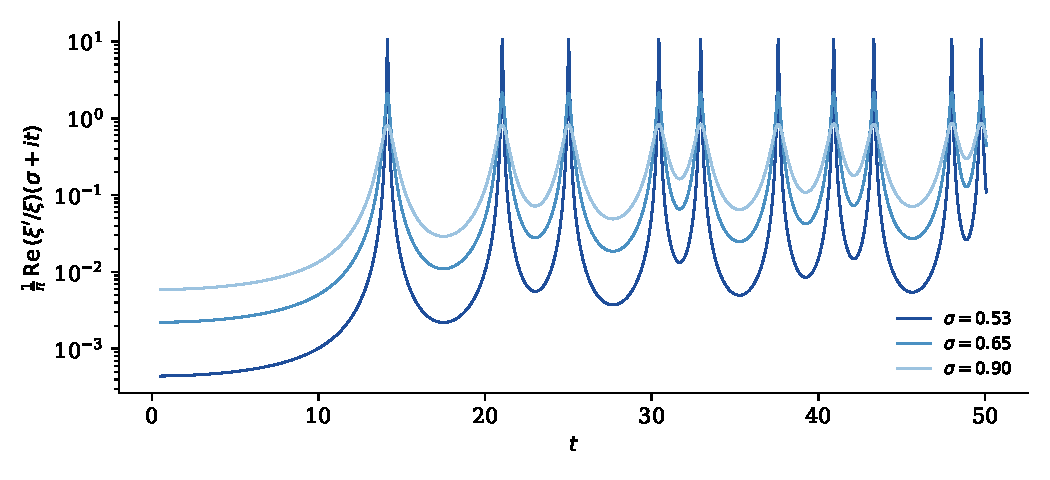
\includegraphics[width=\textwidth]{figs/sf_thorin_strip.pdf}
\caption{The function $\frac1\pi\operatorname{Re}(\xi'/\xi)(\sigma+it)$ of \eqref{eq:sf:closed}, computed from $\zeta'/\zeta$ alone, for $\sigma=0.53,0.65,0.90$ and $0.5\le t\le50$, on a logarithmic vertical scale. Under RH it is the density of $\tau_\sigma$ in the variable $t$, and each zero contributes a Cauchy profile of half width $\sigma-\frac12$ centred at its ordinate, which sharpens into an atom as $\sigma\downarrow\frac12$. The minima on $[0.5,50]$, all at $t=0.5$, are $4.4\times10^{-4}$, $2.2\times10^{-3}$ and $5.9\times10^{-3}$.}
\label{fig:sf:strip}
\end{figure}

\section{Number fields}\label{sec:sf:fields}

\subsection{The constant over $K$}
Theorem \ref{thm:sf:const} extends to every number field, which completes \eqref{eq:sf:alpha1K}.

\begin{theorem}\label{thm:sf:constK}
With the zeros of $\zeta_K$ in the critical strip written $\frac12+i\gamma_\rho$ and summed over all of them with multiplicity,
\[
\kappa_K=A_K+\sum_\rho\Bigl(\frac{2}{1+4\gamma_\rho^2}-\frac{12}{9+4\gamma_\rho^2}\Bigr),
\]
\[
A_K=2+\tfrac12\log|d_K|+r_1\bigl(\log2-\tfrac12\log\pi-\tfrac12\gamma_{\mathrm E}\bigr)+r_2\bigl(2-\gamma_{\mathrm E}-\log2\pi\bigr).
\]
\end{theorem}

\begin{proof}
From the definition of $\xi_K$,
\[
(s-1)\frac{\zeta_K(s)}{\zeta_K(2s)}=2(2s-1)\,|d_K|^{s/2}\,\frac{\Gamma_{\mathbb R}(2s)^{r_1}\Gamma_{\mathbb C}(2s)^{r_2}}{\Gamma_{\mathbb R}(s)^{r_1}\Gamma_{\mathbb C}(s)^{r_2}}\cdot\frac{\xi_K(s)}{\xi_K(2s)} .
\]
The logarithmic derivative of the elementary factor at $s=1$ is $A_K$, using $\psi(1)=-\gamma_{\mathrm E}$, $\psi(\frac12)=-\gamma_{\mathrm E}-2\log2$ and $\psi(2)=1-\gamma_{\mathrm E}$. For the rest, $\frac{\xi_K'}{\xi_K}(\frac12+w)=\sum_\rho\frac{w}{w^2+\gamma_\rho^2}$ over all zeros, taken at $w=\frac12$ minus twice its value at $w=\frac32$.
\end{proof}

For $K=\mathbb Q$ this is Theorem~\ref{thm:sf:const}, whose sum runs over $\operatorname{Re}\gamma_\rho>0$ with doubled weights. For $K=\mathbb Q(i)$, where $\zeta_K=\zeta\cdot L(s,\chi_{-4})$, both sides of the theorem give $\kappa_{\mathbb Q(i)}=1.7846166671\ldots$ to twenty digits when the zero sum is evaluated as $\frac{\xi_K'}{\xi_K}(1)-2\frac{\xi_K'}{\xi_K}(2)$; summed over the zeros below height $1000$, with a tail estimate, it agrees to six digits. The zeros of $\zeta$ and of $L(s,\chi_{-4})$ simply pool their Thorin atoms.

\subsection{A P\'olya kernel for imaginary quadratic fields}
Let $K$ be imaginary quadratic of discriminant $d$, let $a_n=\sum_{m\mid n}\chi_d(m)$ count ideals of norm $n$, and put $\lambda_n=2\pi n/\sqrt{|d|}$ and $F(k)=k(k-2)e^{-k}$. Write $\Lambda_K(s)=(\sqrt{|d|}/2\pi)^s\Gamma(s)\zeta_K(s)$, so that $\xi_K(s)=2s(s-1)\Lambda_K(s)$.

\begin{theorem}\label{thm:sf:kernel}
Let $H_K(x)=\sum_{n\ge1}a_nF(\lambda_nx)$ and $\Phi_K(v)=e^{v/2}H_K(e^v)$. Then $\Phi_K$ is even, decays doubly exponentially, and $\xi_K(\frac12+iz)=2\int_{\mathbb R}\Phi_K(v)e^{izv}dv$. If $|d|<\pi^2$, that is $d\in\{-3,-4,-7,-8\}$, then $\Phi_K>0$; consequently $\xi_K(\frac12+w)/\xi_K(\frac12)$ is the moment generating function of a probability density, and $\zeta_K(\frac12)<0$.
\end{theorem}

\begin{proof}
With $\psi_K(x)=\sum_na_ne^{-\lambda_nx}$ one has $\Lambda_K(s)=\int_0^\infty\psi_K(x)x^{s-1}dx$ and $H_K=(x^2\psi_K')'$, so two integrations by parts give $\int_0^\infty H_K(x)x^{s-1}dx=s(s-1)\Lambda_K(s)=\frac12\xi_K(s)$. Substitute $x=e^v$; the functional equation $\Lambda_K(s)=\Lambda_K(1-s)$ makes $\Phi_K$ even. Every term of $H_K$ is positive for $x>2/\lambda_1=\sqrt{|d|}/\pi$, which covers $x\ge1$ when $|d|<\pi^2$, and evenness covers the rest. Finally $\xi_K(\frac12)=-\frac12\Lambda_K(\frac12)=2\int\Phi_K>0$.
\end{proof}

The sign of $\zeta_K(\frac12)=\zeta(\frac12)L(\frac12,\chi_d)$ is known far beyond these four fields: $L(s,\chi_d)$ has no positive real zero for $-3\cdot10^8\le d<0$ \cite{watkins2004}. For $d=-4$ the Fourier identity holds to sixteen digits at $z=0$ and $z=2.5$. Beyond $|d|<\pi^2$ positivity is arithmetic. Replacing $a_n$ by its mean $L(1,\chi_d)$ makes $H_K(1)$ small, about $L(1,\chi_d)\lambda_1/6$, since $\int_0^\infty F=0$; the sign is decided by how the smallest ideal norms deviate from their average.

\begin{theorem}\label{thm:sf:inert}
If $2$ and $3$ are both inert in $K$, then $\Phi_K$ takes negative values. This holds for infinitely many fields, among them $d=-19,-43,-67,-163$.
\end{theorem}

\begin{proof}
Write $x=y\sqrt{|d|}/2\pi$, so $H_K=\sum_na_nF(ny)$. The ideal counts are multiplicative with $a_{p^e}\le e+1$, and when $2,3$ are inert $a_{2^e}$ and $a_{3^e}$ vanish for odd $e$ and equal $1$ for even $e$. Hence $a_n\le a_n^*$, where $a_n^*=0$ unless $v_2(n)$ and $v_3(n)$ are even, in which case $a_n^*$ is the number of divisors of $n2^{-v_2(n)}3^{-v_3(n)}$; in particular $a_2=a_3=0$. At $y=1.42$, $F(ny)>0$ for $n\ge2$, and
\[
H_K\le F(1.42)+\sum_{n\ge4}a_n^*F(1.42\,n)=-0.19908+0.13918<0,
\]
the sum computed to $n=4000$ with negligible tail. Finally $2$ and $3$ are both inert exactly when $d\equiv5\bmod24$, which holds for infinitely many fundamental discriminants.
\end{proof}

Since $\xi_K$ is a constant multiple of $\xi(s)\Lambda(s,\chi_d)$ (proof of Theorem~\ref{beta:thm:realchar}), $\Phi_K$ is a positive multiple of the convolution of P\'olya's kernel with the theta kernel $v\mapsto e^{3v/2}\vartheta_{\chi_d}(e^{2v})$ of Section~\ref{sec:hitexit}. So for $d=-4$ positivity also follows from Proposition~\ref{beta:prop:kernel}, and when $2$ and $3$ are inert the theta function of $\chi_d$ takes negative values (compare Section~\ref{sec:hitexit}).

All $6079$ fundamental discriminants with $|d|\le20000$ were scanned on a grid of $200$ points (Section~\ref{sec:sf:computing}); $2738$ are positive at every grid point, and a grid ten times finer changes none. Table \ref{tab:sf:kernel} sorts them by the behaviour of $2$ and $3$: the more small primes split, the more ideals of small norm, and the likelier positivity. Positivity is not decided at the centre: only $1904$ of the $3341$ failures have $\Phi_K(0)<0$. The number of positive fields per block of $2000$ discriminants falls from $337$ to between $253$ and $272$ in the last five blocks.

\begin{table}[t]
\centering
\begin{tabular}{lccc}
\toprule
& $\chi_d(3)=1$ & $\chi_d(3)=0$ & $\chi_d(3)=-1$\\
\midrule
$\chi_d(2)=1$ & $676/767$ & $334/507$ & $412/757$\\
$\chi_d(2)=0$ & $489/753$ & $178/514$ & $131/757$\\
$\chi_d(2)=-1$ & $397/761$ & $121/500$ & $0/763$\\
\bottomrule
\end{tabular}
\caption{Fields with $\Phi_K>0$ at every point of the grid of Section~\ref{sec:sf:computing}, among fundamental discriminants $-20000\le d<0$. The empty cell is Theorem \ref{thm:sf:inert}.}
\label{tab:sf:kernel}
\end{table}

\section{Computing the quantities in this chapter}\label{sec:sf:computing}

The sieve and the ideal counts are exact integer computations, done with \texttt{numpy}. The analytic quantities are floating point, computed with \texttt{mpmath} at twenty digits or more unless stated otherwise, and carry no rigorous error bounds.

\begin{itemize}
\item Squarefree indicators to $N$: start from an array of ones and zero out multiples of $d^2$ for $d\le\sqrt N$; cumulative sums give $Q$ exactly, and $\Delta$ in floating point. A sieve to $4\times10^7$ runs in seconds.
\item Tilted P\'olya means: $\E_\theta[T]=\frac12(\xi'/\xi)(\frac12+\frac\theta2)$ by numerical differentiation of $\log\xi$; no quadrature of $\Phi$ is needed. The P\'olya integral itself converges with forty terms of $\Phi$ on $[0,4]$.
\item Atom coefficients $R_\rho$: \texttt{zetazero(k)} and \texttt{diff(zeta,rho)}. Sixty zeros take under a minute.
\item Kernel signs $\Phi_K$: Kronecker symbols by quadratic reciprocity and $a_n$ by a divisor sieve to $12\sqrt{|d|}+50$, both exact; $H_K$ in floating point on $200$ points of $[1,\max(1,\sqrt{|d|}/\pi)]$. This covers $v\ge0$, evenness covers $v<0$, and beyond $\sqrt{|d|}/\pi$ every term is positive.
\item The Thorin density of Figure \ref{fig:sf:strip}: the closed form \eqref{eq:sf:closed}, on a grid refined near the first ten ordinates.
\end{itemize}

\section{The Euler product as a law}\label{sec:sf:euler}

For $\sigma>1$, $P(N=n)=\mu(n)^2n^{-\sigma}/D(\sigma)$ is a law on squarefree integers with $\log N=\sum_pB_p\log p$ for independent Bernoulli variables of success probability $p^{-\sigma}/(1+p^{-\sigma})$. As for the Euler products of Chapter~\ref{ch:09}, $\log\E N^{-w}=\log D(\sigma+w)-\log D(\sigma)$ has a L\'evy Khintchine form, here with the signed L\'evy measure $\sum_p\sum_k(-1)^{k+1}k^{-1}p^{-k\sigma}\delta_{k\log p}$ (compare \eqref{eq:ch09signed}), so by uniqueness the law of $\log N$ is not infinitely divisible; it is quasi infinitely divisible in the sense of \cite{lindnerpansato2018}. The negative part sits at even $k$ and contributes
\[
-\sum_p\sum_{j\ge1}\frac{p^{-2js}}{2j}=-\frac12\log\zeta(2s)
\]
to $\log D(s)$, the factor $\zeta(2s)^{-1/2}$: in $D(s)=\zeta(s)/\zeta(2s)$ the even $k$ carry $+1/k$ from $\zeta(s)$ and $-2/k$ from $1/\zeta(2s)$. The factor $1/\zeta(2s)$, which makes the arithmetic side signed, becomes after the change of variable $u=(2s-\frac12)^2$ the positive Thorin measure of Proposition \ref{prop:sf:thorin} on the analytic side, provided RH holds.

\subsection{Open problems}

\begin{problem}[The exponent one quarter]\label{op:sfquarter}
Prove that $\Delta(x)\ll x^{1/4+\varepsilon}$ on RH; the best exponent known on RH is $\frac{11}{35}$ (end of Section~\ref{sec:sf:thorin}). By Proposition~\ref{prop:sf:gamman} it would follow from removing the factor $n^{1/8}$ at $n\asymp x^2$, and by Corollary~\ref{cor:sf:omega} it amounts to emptying the exceptional set.
\end{problem}

\begin{problem}[How often is $\Phi_K$ positive?]\label{op:sfdensity}
Does the set of negative fundamental discriminants $d$ with $\Phi_K>0$ have positive lower density? Is there a finite set of splitting conditions on small primes under which $\Phi_K>0$ for every $d$ that satisfies them, a positive counterpart of Theorem~\ref{thm:sf:inert}?
\end{problem}

\section{Notes}

The question and both answers are in \cite{mathstackexchange2016}. The results on the size of $\Delta(x)$, unconditional and on RH, are credited where they are used, in and after Corollary~\ref{cor:sf:omega} and at the end of Section~\ref{sec:sf:thorin}. Section~13.2.1 of \cite{montgomeryvaughan2007} sets as exercises the exponents $\frac25$ and $\frac13$ on RH and, for the Ces\`aro weight $1-n/x$, the exponent $\frac14+\varepsilon$, a smoothed statement like one direction of Theorem~\ref{thm:sf:smooth}. Meng \cite{meng2017} studies the distribution of $x^{-1/4}\Delta(x)$ under RH and further hypotheses, and Gorodetsky, Matom\"aki, Radziwi\l\l{} and Rodgers \cite{gmrr2021} prove that RH is equivalent to an essentially sharp bound for the variance of squarefree integers in short intervals. Theorems~\ref{thm:sf:smooth} and~\ref{thm:sf:meansq} follow in a few lines from Mellin inversion, the Paley Wiener theorem and Conrad's descent; we know no source that states them as equivalences.

P\'olya's kernel $\Phi$ goes back to Riemann \cite{riemann1859}; P\'olya \cite{polya1926} studied it with its series, evenness and decay. Its positivity, immediate from the series for $u\ge0$ and evenness, is credited by Biane, Pitman and Yor \cite[Section~2.2]{bpy2001} to Chung and to Newman \cite{newman1976}. They also discuss the Gamma(2) structure of the Bessel hitting times of Section~\ref{sec:sf:gamma2} \cite[(6) to (8) and Table~2]{bpy2001}, through which Williams \cite[Section~5]{williams1990} represents $\xi$. The family $\varphi_\sigma$ and its Thorin densities are Theorem~18 and Remark~21 of \cite{polson2018vdp} and Theorem~\ref{thm:10dshift}, and the positivity criterion of Section~\ref{sec:sf:strip} is due to Hinkkanen \cite{hinkkanen1997} and Lagarias \cite{lagarias1999}. Polson \cite{polson2026thorin} studies the Thorin density of $\xi(\sigma)/\xi(\sigma+s)$ further, with an explicit formula representation, the exact strength of its pointwise positivity and a quasi infinitely divisible factorisation. Stopple \cite{stopple2014} studies the P\'olya kernels of quadratic Dirichlet $L$ functions under the heat flow.

As far as we know, Theorems~\ref{thm:sf:mertens}, \ref{thm:sf:threshold}, \ref{thm:sf:kernel} and \ref{thm:sf:inert} are new. The equivalences with RH in this chapter are reformulations; none of them proves a case of it.

\section{Exercises}

\begin{enumerate}
\item Show that $\kappa=\gamma_{\mathrm E}-2\zeta'(2)/\zeta(2)$, and deduce $\kappa=24\log A-\gamma_{\mathrm E}-2\log2\pi$ from the functional equation and $\zeta'(-1)=\frac1{12}-\log A$, where $A$ is Glaisher's constant.
\item Prove \eqref{eq:sf:g} and $\int_0^\infty g(\theta)\theta^{s-1}d\theta=-(1+s)\Gamma(s)\zeta(s)$ for $0<\operatorname{Re}s<1$, and deduce \eqref{eq:sf:EQ}.
\item Show that $(1+s)\Gamma(s)2^{-s}$ is regular at $s=-1$, and deduce the term $-\pi^2/(3\zeta(3)X)$ in Corollary~\ref{cor:sf:mertens}(iii). Compare it with Table~\ref{tab:sf:EQ} at $X=10^3$, and explain why exponential smoothing (Theorem~\ref{thm:sf:smooth}) gives a term in $\log x/x$ instead.
\item Derive the closed forms of $R_1$ and $R_2$. Show, by comparing the Taylor coefficients of $\sinh^3x=\frac14(\sinh3x-3\sinh x)$ with those of $x^3\cosh x$, that $(\sinh x/x)^p\ge\cosh x$ for all real $x$ if and only if $p\ge3$, and that $f_V(v)=v^2/60+O(v^4)$ as $v\to0$.
\item Show that $h^{(\delta)}_c$ is a probability density, that $2t\,h^{(\delta)}_c(t^2)$ is the sum of two Poisson kernels, and that near $r=c$ it is a Cauchy density of half width $2\delta\sqrt c$ up to a relative error $O(\delta/\sqrt c)$.
\item Show that for no $\sigma>\frac12$ is $u\mapsto1/D(\sigma+\sqrt u)$ the Laplace transform of a positive measure: for $\sigma>1$ it increases from $1/D(\sigma)$ to $1$, for $\sigma=1$ it vanishes at $u=0$, and for $\frac12<\sigma<1$ it is negative at $u=0$ and vanishes at $u=(1-\sigma)^2$. For $\sigma>1$, show that $D(\sigma+\sqrt u)/D(\sigma)$ is the Laplace transform of the first passage time of a Brownian motion to the independent level $\log N/\sqrt2$, with $N$ as in Section~\ref{sec:sf:euler}, and that it is not a GGC transform, since it does not tend to $0$ as $u\to\infty$.
\item Show that a zero of $\zeta_K$ at $s=\frac12$ of order $2m$ adds $\frac{4m}3$ to the zero sum of Theorem~\ref{thm:sf:constK}. For $K=\mathbb Q(i)$, show with the duplication formula that $\xi_K=\frac2{\sqrt\pi}\,\xi\,\Lambda$ (with $\xi_K$ as in this chapter, four times that of Chapter~\ref{ch:beta}), with $\Lambda$ the completed $\beta$ function of Chapter~\ref{ch:beta}, and deduce from Proposition~\ref{beta:prop:kernel} and the positivity of P\'olya's kernel that $\Phi_K>0$.
\item Show that $2$ and $3$ are both inert in $\mathbb Q(\sqrt d)$ if and only if $d\equiv5\bmod24$ and that $a_n\le a_n^*$ in the proof of Theorem~\ref{thm:sf:inert}, and check by machine that $F(1.42)=-0.19908$ and $\sum_{n\ge4}a_n^*F(1.42\,n)=0.13918$.
\end{enumerate}

\section{Open computational problems}

\begin{compproblem}[The squarefree error beyond $10^{18}$]\label{cp:sferror}
Objective: extend by one decade the computation of Mossinghoff, Oliveira e Silva and Trudgian \cite{mot2021}, who found $-1.12543\,x^{1/4}<\Delta(x)<1.11653\,x^{1/4}$ for all $0<x\le10^{18}$ (their sparse samples up to $10^{28}$ stay below $1.2$), and compare the extremes with the atom sums of Figure~\ref{fig:sf:atoms}. Objects and scale: the extremes of $\Delta(x)/x^{1/4}$ for $10^{18}<x\le10^{19}$, by a segmented sieve of $\mu^2$, and the sums $1+2\operatorname{Re}\sum_{k\le K}R_{\rho_k}x^{\rho_k/2}$ of \eqref{eq:sf:Rrho} with $K=10^4$ at the extreme points. Route: integer arithmetic for $Q$ in two independent implementations, checked at sparse points against Pawlewicz's algorithm \cite{pawlewicz2011}; zeros from the LMFDB \cite{lmfdb} or PARI/GP \cite{pari2023}, and $R_\rho$ in ball arithmetic. Deliverable: the record values of $|\Delta(x)|/x^{1/4}$ with their locations, and the agreement of the atom sums with $\Delta(x)/x^{1/4}$ there as a function of $K$. Why it matters: up to $10^{18}$ the values of $|\Delta(x)|/x^{1/4}$ stay below $1.12543$, far below the proved $\limsup\Delta(x)/x^{1/4}>3$; the computation measures how slowly the oscillations forced by the zeros appear, against the limiting distribution studied by Meng \cite{meng2017}.
\end{compproblem}

\begin{compproblem}[Oscillations of squarefree ideals]\label{cp:sfideals}
Objective: for $K=\mathbb Q(i)$ and $\mathbb Q(\sqrt{-3})$ let $\Delta_K(x)=Q_0(x)-c_Kx/\zeta_K(2)$ be the error in the count of squarefree ideals, the case $\alpha=0$ of \eqref{eq:sf:perron}. Landau's argument of Corollary~\ref{cor:sf:omega}, applied to $\zeta_K(s)/\zeta_K(2s)$, whose poles at $\rho/2$ come from the zeros of $\zeta$ and of $L(s,\chi_d)$, gives $\Delta_K(x)=\Omega(x^{1/4})$; prove explicit bounds $\limsup\Delta_K(x)/x^{1/4}>b_K$ and $\liminf\Delta_K(x)/x^{1/4}<-b_K$ and find the extreme values. Objects and scale: the residues of $\zeta_K(s)x^s/(s\,\zeta_K(2s))$ at the poles $\rho/2$ given by the first $2000$ zeros of $\zeta$ and of $L(s,\chi_d)$; counts of squarefree ideals of norm up to $10^{14}$. Route: the method of \cite{mot2021}, that is Ingham's argument with many zeros and lattice reduction to establish a weak independence of the pooled ordinates; for the counts, a segmented sieve on norms, the number of squarefree ideals of norm $n$ being determined by the factorisation of $n$ and the splitting of its primes. Deliverable: constants $b_K$ with the computations that prove them, and the extreme values of $\Delta_K(x)/x^{1/4}$ up to $10^{14}$ with their locations. Why it matters: the zeros of $\zeta$ and of $L(s,\chi_d)$ pool their atoms (Theorem~\ref{thm:sf:constK}), and the oscillations test whether the pooled ordinates behave independently; we found no Omega result and no computation of the extremes of $\Delta_K$ for these fields in the literature.
\end{compproblem}

\begin{compproblem}[P\'olya kernels of imaginary quadratic fields]\label{cp:sfkernel}
Objective: extend Table~\ref{tab:sf:kernel} and prove its entries. Objects and scale: all fundamental discriminants $-10^7\le d<0$. Route: $a_n$ by a divisor sieve; $H_K$ on $[1,\sqrt{|d|}/\pi]$, beyond which every term is positive and below which evenness applies, in interval arithmetic with a bound on the derivative between grid points, so that positivity is proved and not sampled. Deliverable: proved counts of the fields with $\Phi_K>0$ in dyadic ranges of $|d|$ and by the splitting of $2$, $3$, $5$ and $7$, and the splitting types, if any, for which every field in range is positive. Why it matters: positivity of $\Phi_K$ makes $\xi_K(\frac12+w)/\xi_K(\frac12)$ a moment generating function (Theorem~\ref{thm:sf:kernel}); Theorem~\ref{thm:sf:inert} gives infinitely many fields with sign changes, and whether the positive fields have positive density is Open Problem~\ref{op:sfdensity}. Problem~\ref{cp:hitexit} asks the same question for the theta functions of the characters $\chi_d$, from which $\Phi_K$ is obtained by convolution with P\'olya's kernel.
\end{compproblem}

\begin{compproblem}[P\'olya kernels of real quadratic fields]\label{cp:sfreal}
Objective: construct the analogue of Theorem~\ref{thm:sf:kernel} for real quadratic fields and compute its signs. Objects and scale: fundamental discriminants $0<d\le10^5$. Route: since $\int_0^\infty K_0(2y)y^{s-1}dy=\Gamma(s/2)^2/4$, the completed function $d^{s/2}\Gamma_{\mathbb R}(s)^2\zeta_K(s)$ is the Mellin transform of $\psi_K(x)=4\sum_na_nK_0(2\pi nx/\sqrt d)$; put $H_K=(x^2\psi_K')'$ and $\Phi_K(v)=e^{v/2}H_K(e^v)$, evaluate $K_0$ by its series and asymptotic expansion, and decide signs in interval arithmetic. As in Section~\ref{sec:sf:fields}, $\Phi_K$ is also the convolution of P\'olya's kernel with the theta kernel of the even character $\chi_d$ (proof of Theorem~\ref{beta:thm:realchar}), whose sign can be computed separately; positive real zeros of such theta functions are studied in \cite{louboutinmunsch2013}. Deliverable: the set of $d$ with $\Phi_K>0$ sorted by the splitting of $2$ and $3$, the first $d$ with a negative value, and, if sign changes persist when $2$ and $3$ are inert, an explicit point and bound as in the proof of Theorem~\ref{thm:sf:inert}. Why it matters: the Bessel kernel changes the archimedean side and keeps the arithmetic one, and a negative value of the theta kernel can be smoothed away by the convolution, so the computation separates the sources of sign changes.
\end{compproblem}

\chapter[Dirichlet Beta and the Gaussian Field]{The Dirichlet Beta Function and the Gaussian Field}\label{ch:beta}

The unitary automorphic representations of $\mathrm{GL}(1)$ over $\mathbb Q$ are, up to twists by $\lvert\cdot\rvert^{it}$, the primitive Dirichlet characters, and one of the simplest nontrivial ones is the character $\chi_{-4}$ of the Gaussian field $K=\mathbb Q(i)$: $\chi_{-4}(n)=0$ for even $n$, $\chi_{-4}(n)=1$ for $n\equiv1$ and $\chi_{-4}(n)=-1$ for $n\equiv3\pmod 4$. Its $L$ function is the Dirichlet beta function
\begin{equation}\label{beta:eq:beta}
\beta(s)=\sum_{n\ge 0}\frac{(-1)^n}{(2n+1)^s}=\sum_{n\ge1}\frac{\chi_{-4}(n)}{n^s}
=\prod_{p}\bigl(1-\chi_{-4}(p)p^{-s}\bigr)^{-1},\qquad \operatorname{Re} s>1,
\end{equation}
with $\beta(1)=\pi/4$ and $\beta(2)=0.9159656$, Catalan's constant. Since $\chi_{-4}$ is real, odd and primitive with root number one, the completed function
\begin{equation}\label{beta:eq:Lambda}
\Lambda(s)=\Bigl(\frac{4}{\pi}\Bigr)^{s/2}\Gamma\Bigl(\frac{s+1}{2}\Bigr)\beta(s)
\end{equation}
is entire of order one with $\Lambda(s)=\Lambda(1-s)$. The generalized Riemann hypothesis (GRH) for $\beta$ asserts that every zero of $\Lambda$ lies on $\operatorname{Re} s=\tfrac12$.

This chapter works out for $\beta$ the Thorin framework of Chapters~\ref{ch:10b} and \ref{ch:10d} \cite{polson2017,polson2018vdp}. For real primitive characters the closed form of the Thorin density, the GGC property to the right of the critical strip and the equivalence of GRH with the GGC property at every basepoint $\alpha>\frac12$ are Theorem~30 and Remark~32 of \cite{polson2018vdp}, and in this book they are the case of $\chi_{-4}$ of Theorem~\ref{thm:10dshift}; what $\beta$ adds is an explicit positive kernel, a signed L\'evy measure, and the question of what the signs of that measure can prove. The framework has three parts: a L\'evy form of the completed function to the right of the critical strip; the $2\sin^2$ lemma of Chapter~\ref{ch:10d} (Lemma~\ref{lem:10dsin2}, from \cite{polson2018vdp}), which turns the L\'evy measure of the primal function into the Thorin measure of its reciprocal; and Thorin's condition, that $\Lambda(\tfrac12)/\Lambda(\tfrac12+\sqrt v)$ is the Laplace transform of a generalized gamma convolution (GGC, Definition~\ref{def:ch10ggc}), whose analyticity in the cut plane excludes zeros off the critical line (Theorem~\ref{thm:10bmain}).

Three features make $\beta$ the natural first case beyond $\zeta$. Its Mellin kernel is the weight $3/2$ theta series $\eta^3$, positive by the product formula. Its prime atoms carry the weights $\chi_{-4}(n)\Lambda(n)$, negative at $3,7,11,19,\dots$, so Thorin positivity is no longer termwise but arithmetic. Finally $\zeta_K=\zeta\cdot\beta$: the trivial character of $\mathrm{GL}(1)$ over $K$ induces to the isobaric representation $1\boxplus\chi_{-4}$ of $\mathrm{GL}(2)$ over $\mathbb Q$, and Thorin densities respect this decomposition.

Sections~\ref{beta:sec:primal} to \ref{beta:sec:lemma} construct the primal law, the L\'evy form and the closed form $T_\alpha(y)=\operatorname{Re}(\Lambda'/\Lambda)(\alpha+i\sqrt y)/(2\pi\sqrt y)$ of the Thorin density. Sections~\ref{beta:sec:uncond} and \ref{beta:sec:grh} recall the GGC property for $\alpha\ge1$ and the equivalence of GRH with the GGC property for all $\alpha>\tfrac12$. Section~\ref{beta:sec:gauss} treats the Gaussian field and the limits of termwise bounds; Section~\ref{beta:sec:axis} shows that positivity is free on the real axis, can fail only in short windows, and that GRH is equivalent to the density on each line $\tfrac12<\operatorname{Re} s\le1$ being smallest on the real axis; Section~\ref{beta:sec:argument} identifies the Thorin measure with the argument of $\Lambda$. Sections~\ref{beta:sec:centre} and \ref{beta:sec:eta} treat the centre and the pair $(\eta,\chi_{12})$.


\section{The completed beta function and its primal law}\label{beta:sec:primal}

\subsection{The eta cube kernel}
Jacobi's identity gives, with $q=e^{2\pi i\tau}$,
\begin{equation}\label{beta:eq:jacobi}
\eta(\tau)^3=q^{1/8}\prod_{m\ge1}(1-q^m)^3=\sum_{n\ge0}(-1)^n(2n+1)q^{(2n+1)^2/8}.
\end{equation}
At $\tau=ix$ this is the theta series of $\chi_{-4}$,
\begin{equation}\label{beta:eq:theta}
\vartheta_\beta(x):=\eta(ix)^3=\sum_{n\ge1}\chi_{-4}(n)\,n\,e^{-\pi n^2x/4},
\end{equation}
and $\eta(i/x)=\sqrt x\,\eta(ix)$ gives $\vartheta_\beta(1/x)=x^{3/2}\vartheta_\beta(x)$.

\begin{proposition}[Mellin form; classical]\label{beta:prop:mellin}
For all $s\in\C$,
\begin{equation}\label{beta:eq:mellin}
\Lambda(s)=\frac{\sqrt\pi}{2}\int_0^\infty x^{(s-1)/2}\,\eta(ix)^3\,dx .
\end{equation}
\end{proposition}

\begin{proof}
For $\operatorname{Re} s>1$ integrate \eqref{beta:eq:theta} term by term, using
\[
\int_0^\infty x^{(s+1)/2-1}e^{-\pi n^2x/4}\,dx=\Gamma\Bigl(\frac{s+1}{2}\Bigr)\Bigl(\frac{4}{\pi n^2}\Bigr)^{(s+1)/2}
\]
and $\sum_n\chi_{-4}(n)\,n^{-s}=\beta(s)$; the result is $(4/\pi)^{(s+1)/2}\Gamma(\tfrac{s+1}{2})\beta(s)$, which equals $(2/\sqrt\pi)\Lambda(s)$. Since $\vartheta_\beta$ decays like $e^{-\pi x/4}$ at infinity and like $x^{-3/2}e^{-\pi/(4x)}$ at zero, the integral is entire.
\end{proof}

\begin{proposition}[Primal kernel]\label{beta:prop:kernel}
The function $\Phi_\beta(u)=e^{3u/2}\,\eta(ie^{2u})^3$ is even, strictly positive, and decays like $\exp(\tfrac32|u|-\tfrac\pi4e^{2|u|})$. For all $w\in\C$,
\begin{equation}\label{beta:eq:kernel}
\Lambda\bigl(\tfrac12+w\bigr)=\sqrt\pi\int_{-\infty}^{\infty}e^{wu}\Phi_\beta(u)\,du
=2\sqrt\pi\int_0^\infty\cosh(wu)\,\Phi_\beta(u)\,du .
\end{equation}
\end{proposition}

\begin{proof}
Evenness is the transformation law, and positivity is the product in \eqref{beta:eq:jacobi}, every factor $1-q^m$ being positive for $q=e^{-2\pi x}\in(0,1)$. The identity is \eqref{beta:eq:mellin} after $x=e^{2u}$.
\end{proof}

This is the theta series proof of the functional equation for odd characters \cite{iwanieckowalski2004}; the eta cube form is in \cite[Section~8.1]{polson2018vdp}, and the theta identity is recalled in Chapter~\ref{ch:11}. Up to normalisation, $\Phi_\beta$ is the P\'olya kernel of Lemma~\ref{lem:10bkernel} for $\Xi^{\mathrm{sd}}$, here $\Lambda(\tfrac12+z)$ up to a constant factor, and it is positive for the reason given after that lemma for eta products, whereas the positivity of the Riemann P\'olya kernel takes work; and unlike $\xi$, $\Lambda$ has no polar factor. The normalised kernel $\Phi_\beta/\int\Phi_\beta$ is the density of a symmetric random variable $X_\beta$, the P\'olya variable of $\Xi^{\mathrm{sd}}$, which we call the \emph{primal law}, with
\begin{equation}\label{beta:eq:primal}
\E\bigl[e^{wX_\beta}\bigr]=\frac{\Lambda(\tfrac12+w)}{\Lambda(\tfrac12)},\qquad
\E\bigl[e^{itX_\beta}\bigr]=\frac{\Lambda(\tfrac12+it)}{\Lambda(\tfrac12)} .
\end{equation}
Numerically $\Lambda(\tfrac12)=0.86913481$, $\beta(\tfrac12)=0.66769146$ and $\Phi_\beta(0)=0.45338383$.

\subsection{Zeros and the tilt}

\begin{lemma}[No real zeros]\label{beta:lem:real}
$\beta(\sigma)\ge1-3^{-\sigma}>0$ for real $\sigma>0$. Hence $\Lambda$ has no zeros in $(0,1)$.
\end{lemma}

\begin{proof}
For $\sigma>0$ the series \eqref{beta:eq:beta} converges, alternates and has strictly decreasing terms.
\end{proof}

The zeros $\rho$ of $\Lambda$ are symmetric under $\rho\mapsto1-\rho$ and $\rho\mapsto\bar\rho$, and every zero satisfies $0<\operatorname{Re}\rho<1$ (the Euler product excludes $\operatorname{Re} s>1$, and the nonvanishing of $\beta$ on $\operatorname{Re} s=1$ with the functional equation excludes the edges). Writing $\rho=\tfrac12+i\theta$ (by Lemma~\ref{beta:lem:real} no $\theta$ is purely imaginary, so the condition $\operatorname{Re}\theta>0$ picks one of each pair $\pm\theta$), the functional equation gives $\Lambda'(\tfrac12)=0$ and kills the exponential factor of the Hadamard product, so
\begin{equation}\label{beta:eq:hadamard}
\frac{\Lambda(\tfrac12+w)}{\Lambda(\tfrac12)}=\prod_{\operatorname{Re}\theta>0}\Bigl(1+\frac{w^2}{\theta^2}\Bigr),
\qquad
\operatorname{Re}\frac{\Lambda'}{\Lambda}(s)=\sum_{\rho}\frac{\operatorname{Re} s-\operatorname{Re}\rho}{|s-\rho|^2},
\end{equation}
the sum converging absolutely since $\sum|\rho|^{-2}<\infty$. Under GRH every $\theta$ is a real ordinate $\gamma$ and $\Lambda(\tfrac12)/\Lambda(\tfrac12+w)=\prod_{\gamma>0}\gamma^2/(\gamma^2+w^2)$, the product \eqref{eq:10batoms} of Chapter~\ref{ch:10b} for $\Xi^{\mathrm{sd}}$. The first ordinates $\gamma$ are $6.02094890$, $10.24377030$, $12.98809801$, $16.34260710$ and $18.29199320$. We write
\begin{equation}\label{beta:eq:calpha}
c_\alpha:=\frac{\Lambda'}{\Lambda}(\alpha)=\tfrac12\log\frac4\pi+\tfrac12\psi\Bigl(\frac{\alpha+1}{2}\Bigr)+\frac{\beta'}{\beta}(\alpha)
\end{equation}
and $V:=(\log\Lambda)''(\tfrac12)=\mathrm{Var}(X_\beta)=0.156030$, twice the sum $S_1=0.078015$ of Table~\ref{tab:10bcatalogue}. By \eqref{beta:eq:hadamard}, $c_\alpha>0$ for $\alpha\ge1$, and $c_{1/2}=0$.


\section{The L\'evy form for \texorpdfstring{$\alpha>1$}{alpha > 1}}\label{beta:sec:levy}

\begin{theorem}[L\'evy form; as in Section~\ref{sec:10daway}]\label{beta:thm:levy}
For $\alpha>1$ and $\operatorname{Re} s\ge0$,
\begin{equation}\label{beta:eq:levy}
\log\frac{\Lambda(\alpha+s)}{\Lambda(\alpha)}-c_\alpha s=\int_0^\infty\bigl(e^{-sx}-1+sx\bigr)e^{-\alpha x}\,\frac{\mu_\beta(dx)}{x},
\end{equation}
with the signed measure
\begin{equation}\label{beta:eq:mubeta}
\mu_\beta(dx)=\frac{dx}{2\sinh x}+\sum_{n\ge2}\chi_{-4}(n)\,\Lambda(n)\,\delta_{\log n}(dx).
\end{equation}
\end{theorem}

\begin{proof}
The factor $(4/\pi)^{s/2}$ is absorbed by the tilt. For $\operatorname{Re} z>0$,
\[
\log\frac{\Gamma(z+v)}{\Gamma(z)}-v\psi(z)=\int_0^\infty\bigl(e^{-vx}-1+vx\bigr)\frac{e^{-zx}}{x(1-e^{-x})}\,dx,
\]
since both sides and their first derivatives vanish at $v=0$ and both have second derivative $\psi'(z+v)$. Taking $z=\tfrac{\alpha+1}{2}$, $v=\tfrac s2$ and $x\mapsto2x$ turns the kernel into $e^{-\alpha x}/(2x\sinh x)$. For the Dirichlet series, on $\operatorname{Re} s>1$ the function $\log\beta(s)$ is $\sum_{n\ge2}\chi_{-4}(n)\Lambda(n)(\log n)^{-1}n^{-s}$, which gives the atoms. Absolute convergence follows from $|e^{-sx}-1+sx|\le\min(2+|s|x,\tfrac12|s|^2x^2)$.
\end{proof}

With the prime sum truncated at $n\le2\times10^5$ the two sides of \eqref{beta:eq:levy} agree to seven digits at $(\alpha,s)=(2,2)$ and to twelve at $(3,2)$, where both equal $0.232881325700$.

\begin{remark}[Comparison with $\xi$]\label{beta:rem:xi}
For $\xi(s)=\tfrac12s(s-1)\pi^{-s/2}\Gamma(\tfrac s2)\zeta(s)$ the same computation gives the measure $-e^x\,dx+dx/(e^{2x}-1)+\sum_{n\ge2}\Lambda(n)\delta_{\log n}$. The polar factor $\alpha-1+s$ is log concave in $s$, so it enters with a negative sign (Section~\ref{sec:10daway}). For $\beta$ there is no polar term, the archimedean density is $1/(2\sinh x)$ (an odd character shifts the gamma argument by one half), and the prime part is the difference of two positive measures, carried by the prime powers $n\equiv1$ and $n\equiv3\pmod4$ respectively.
\end{remark}


\section{The \texorpdfstring{$2\sin^2$}{2 sin squared} lemma and the Thorin density}\label{beta:sec:lemma}

Lemma~\ref{lem:10dsin2} transports a positive L\'evy measure. The transport is linear in the measure, and it holds for a signed measure once the positivity conclusion is dropped; we state it in the Laplace variable $v=s^2$ and prove it by Fourier inversion, which also gives \eqref{beta:eq:logformula}.

\begin{lemma}[$2\sin^2$ lemma, signed form; after Lemma~\ref{lem:10dsin2}]\label{beta:lem:2sin2}
Let $f$ be analytic and nonvanishing near $[\alpha,\infty)$, let $c=f'(\alpha)/f(\alpha)$, and suppose that for $s\ge0$
\[
\log\frac{f(\alpha+s)}{f(\alpha)}-cs=\int_0^\infty\bigl(e^{-sx}-1+sx\bigr)\,m(dx)
\]
for a signed measure $m$ with $\int\min(x,x^2)\,|m|(dx)<\infty$. Put
\begin{equation}\label{beta:eq:Tdef}
T(y)=\frac{1}{2\pi\sqrt y}\Bigl[c+\int_0^\infty2\sin^2\Bigl(\frac{x\sqrt y}{2}\Bigr)x\,m(dx)\Bigr],\qquad y>0.
\end{equation}
Then for every $v>0$,
\begin{equation}\label{beta:eq:thorinrep}
\frac{f(\alpha)}{f(\alpha+\sqrt v)}=\exp\Bigl(-\int_0^\infty\log\Bigl(1+\frac vy\Bigr)T(y)\,dy\Bigr).
\end{equation}
The map $m\mapsto T$ is linear and positivity preserving, and $c\ge0$ contributes the positive stable part $c/(2\pi\sqrt y)$.
\end{lemma}

\begin{proof}
With $y=t^2$, $T(y)\,dy=\pi^{-1}\bigl[c+\int x(1-\cos tx)\,m(dx)\bigr]dt$. The integrals
\[
\int_0^\infty\log\Bigl(1+\frac{v}{t^2}\Bigr)dt=\pi\sqrt v,\qquad
\int_0^\infty\log\Bigl(1+\frac{v}{t^2}\Bigr)\cos(xt)\,dt=\frac{\pi}{x}\bigl(1-e^{-x\sqrt v}\bigr),
\]
the second by parts from $\int_0^\infty\sin(xt)\,dt/(t(t^2+v))=\pi(1-e^{-x\sqrt v})/(2v)$, give
\begin{align*}
\int_0^\infty\log\Bigl(1+\frac vy\Bigr)T(y)\,dy
&=c\sqrt v+\int_0^\infty\bigl(e^{-x\sqrt v}-1+x\sqrt v\bigr)m(dx)\\
&=\log\frac{f(\alpha+\sqrt v)}{f(\alpha)} ,
\end{align*}
Fubini being justified by $|1-\cos tx|\le\min(2,t^2x^2/2)$.
\end{proof}

If $f$ is analytic on $\operatorname{Re} s\ge\alpha$, differentiating the L\'evy form at $s=it$ gives $\operatorname{Re}(f'/f)(\alpha+it)-c=\int x(1-\cos tx)\,m(dx)$, so the bracket in \eqref{beta:eq:Tdef} is $\operatorname{Re}(f'/f)(\alpha+i\sqrt y)$. For $f=\Lambda$ this is the main formula of the chapter.

\begin{theorem}[Thorin density of the reciprocal beta function; \cite{polson2018vdp}, Theorem~30]\label{beta:thm:thorin}
For $\alpha>1$ and $v>0$,
\begin{equation}\label{beta:eq:thorinbeta}
\frac{\Lambda(\alpha)}{\Lambda(\alpha+\sqrt v)}=\exp\Bigl(-\int_0^\infty\log\Bigl(1+\frac vy\Bigr)T_\alpha(y)\,dy\Bigr),
\end{equation}
where
\begin{align}
T_\alpha(y)&=\frac{1}{2\pi\sqrt y}\Bigl[c_\alpha+\int_0^\infty2\sin^2\Bigl(\frac{x\sqrt y}{2}\Bigr)e^{-\alpha x}\mu_\beta(dx)\Bigr]\label{beta:eq:Tsin}\\
&=\frac{c_\alpha+G_\alpha(\sqrt y)+P_\alpha(\sqrt y)}{2\pi\sqrt y}
=\frac{1}{2\pi\sqrt y}\,\operatorname{Re}\frac{\Lambda'}{\Lambda}\bigl(\alpha+i\sqrt y\bigr),\label{beta:eq:Tclosed}
\end{align}
with the archimedean and prime parts
\begin{align*}
G_\alpha(t)&=\tfrac12\Bigl[\operatorname{Re}\,\psi\Bigl(\frac{\alpha+1+it}{2}\Bigr)-\psi\Bigl(\frac{\alpha+1}{2}\Bigr)\Bigr]\ge0,\\
P_\alpha(t)&=\sum_{n\ge2}\chi_{-4}(n)\Lambda(n)\,n^{-\alpha}\bigl(1-\cos(t\log n)\bigr).
\end{align*}
Equivalently,
\begin{equation}\label{beta:eq:logformula}
\log\frac{\Lambda(\alpha+\sqrt v)}{\Lambda(\alpha)}=\frac1\pi\int_0^\infty\log\Bigl(1+\frac{v}{t^2}\Bigr)\,\operatorname{Re}\frac{\Lambda'}{\Lambda}(\alpha+it)\,dt .
\end{equation}
\end{theorem}

\begin{proof}
Apply Lemma~\ref{beta:lem:2sin2} to Theorem~\ref{beta:thm:levy}. The density satisfies $T_\alpha(y)\sim c_\alpha/(2\pi\sqrt y)$ as $y\to0$, and $T_\alpha(y)=O(\log y/\sqrt y)$ as $y\to\infty$ because $P_\alpha$ is bounded and $\operatorname{Re}\,\psi(\tfrac{\alpha+1+it}{2})\sim\log(t/2)$.
\end{proof}

In the notation of Theorem~\ref{thm:10dshift}, whose $\Xi_\pi$ is $\Lambda(\tfrac12+z)^2$ up to a constant factor, $2T_\alpha=V_{\alpha-1/2}$, and $T_\alpha(y)\,dy$ is the Thorin measure $\tau$ (Definition~\ref{def:ch10ggc}) of $\Lambda(\alpha)/\Lambda(\alpha+\sqrt v)$ when every zero of $\Lambda$ has real part less than $\alpha$ (for every $\alpha\ge1$ by part~(iii) of that theorem, and for every $\alpha>\frac12$ under GRH).

The sine squared form \eqref{beta:eq:Tsin}, with primes to $2\times10^5$, and the closed form \eqref{beta:eq:Tclosed} give the same values of $2\pi t\,T_\alpha(t^2)$, namely $0.2353511$, $0.7691193$ and $0.32628$ at $(\alpha,t)=(2,1),(2,7),(\tfrac32,4)$. Formula \eqref{beta:eq:logformula} at $(\alpha,v)=(2,1)$, by quadrature to $t=150$ plus the archimedean tail $v(\log(2T/\pi)+1)/(2\pi T)$ at $T=150$, gives $0.2977961$ against $\log\Lambda(3)/\Lambda(2)=0.2977947$; the residual comes from the oscillating prime part beyond $t=150$.


\section{What holds unconditionally}\label{beta:sec:uncond}

\begin{theorem}[GGC for $\alpha\ge1$; Theorem~\ref{thm:10dshift}(iii)]\label{beta:thm:uncond}
For every $\alpha\ge1$ there is a GGC random variable $H^\beta_\alpha\ge0$, with drift zero and Thorin density $T_\alpha>0$ given by \eqref{beta:eq:Tclosed}, such that
\[
\frac{\Lambda(\alpha)}{\Lambda(\alpha+\sqrt v)}=\E\bigl[e^{-vH^\beta_\alpha}\bigr],\qquad v>0.
\]
In particular $\tfrac{\sqrt\pi}{2}\big/\Lambda(1+\sqrt v)$ is a GGC Laplace transform.
\end{theorem}

\begin{proof}
Since every zero has $\operatorname{Re}\rho<1$, each term of \eqref{beta:eq:hadamard} is positive on $\operatorname{Re} s=\alpha\ge1$, so $T_\alpha>0$. By Theorem~\ref{thm:10dshift}(iii) with $a=\alpha-\frac12$, the square $(\Lambda(\alpha)/\Lambda(\alpha+\sqrt v))^2$ is the transform of a GGC with drift zero and Thorin density $V_{\alpha-1/2}=2T_\alpha$, so by Definition~\ref{def:ch10ggc} its square root is the transform of a GGC with drift zero and Thorin density $T_\alpha$. For $\alpha>1$ this is also Theorem~\ref{beta:thm:thorin}.
\end{proof}

The proof uses the zeros rather than the L\'evy measure. On the L\'evy side the sine squared integrand in \eqref{beta:eq:Tsin} is signed, and bounding the atoms by their absolute values proves positivity at every height only above a threshold $\alpha_c$. Write
\begin{align}
A_\alpha(t)&=\tfrac12\log\frac4\pi+\tfrac12\operatorname{Re}\,\psi\Bigl(\frac{\alpha+1+it}{2}\Bigr),\notag\\
S(\alpha)&=\sum_{n\text{ odd}}\Lambda(n)n^{-\alpha}=-\frac{\zeta'}{\zeta}(\alpha)-\frac{\log2}{2^\alpha-1},\label{beta:eq:AS}
\end{align}
so that $\operatorname{Re}\,\Lambda'/\Lambda(\alpha+it)=A_\alpha(t)+\operatorname{Re}\,\beta'/\beta(\alpha+it)$ and $|\beta'/\beta(\alpha+it)|\le S(\alpha)$ for $\alpha>1$.

\begin{proposition}[Termwise positivity]\label{beta:prop:crude}
$A_\alpha(t)$ increases in $t$, $A_\alpha(0)$ increases in $\alpha$, and $S(\alpha)$ decreases. Let $\alpha_c$ be the root of $A_\alpha(0)=S(\alpha)$, numerically $\alpha_c=2.28231064$. For $\alpha\ge\alpha_c$ the bound $A_\alpha(t)-S(\alpha)$ proves $T_\alpha(t^2)>0$ for all $t>0$; for $1<\alpha<\alpha_c$ it fails near $t=0$, although $T_\alpha>0$ by Theorem~\ref{beta:thm:uncond}.
\end{proposition}

\begin{proof}
Monotonicity in $t$ follows from $\operatorname{Re}\,\psi(x+iy)-\psi(x)=\sum_{k\ge0}y^2/\bigl((x+k)((x+k)^2+y^2)\bigr)$; $\psi$ increases on $(0,\infty)$, and $S$ is a Dirichlet series with positive coefficients.
\end{proof}

At $\alpha=\tfrac32$ (Figure~\ref{beta:fig:thorin}, right) the prime part $P_\alpha$ is negative over most of $[0,30]$, with minimum $-0.532$ near $t=19.9$, where $c_\alpha+G_\alpha=1.418$. For $\zeta$ the corresponding prime part is a positive sum.

\begin{figure}[t]
\centering
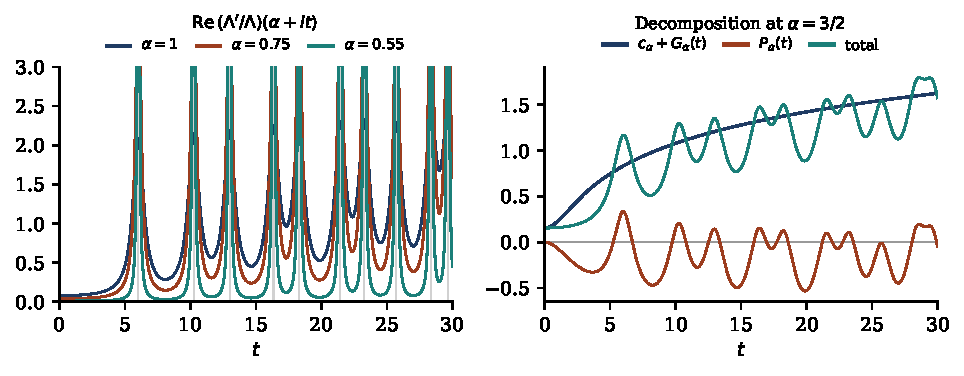
\includegraphics[width=\textwidth]{figs/beta_thorin.pdf}
\caption{Left: $\operatorname{Re}(\Lambda'/\Lambda)(\alpha+it)=2\pi t\,T_\alpha(t^2)$ for $\alpha=1,\,0.75,\,0.55$ and $0\le t\le30$, with the vertical axis cut at $3$; grey lines mark the ordinates of the zeros of $\beta$. As $\alpha\downarrow\frac12$ the density concentrates on the zeros. Right: at $\alpha=\frac32$, the archimedean part with the constant, $c_\alpha+G_\alpha$, the signed prime part $P_\alpha$, and their sum (labelled total).}
\label{beta:fig:thorin}
\end{figure}


\section{GRH as Thorin positivity}\label{beta:sec:grh}

\begin{theorem}[GRH as Thorin positivity; Theorem~\ref{thm:10dshift}(iv) and \cite{polson2018vdp}, Remark~32]\label{beta:thm:grh}
The following are equivalent.
\begin{enumerate}
\item[(i)] GRH for $\beta$.
\item[(ii)] For every $\alpha>\tfrac12$, $\Lambda(\alpha)/\Lambda(\alpha+\sqrt v)$ is the Laplace transform of a GGC.
\item[(iii)] $\operatorname{Re}\,(\Lambda'/\Lambda)(s)>0$ for $\operatorname{Re} s>\tfrac12$.
\end{enumerate}
In this case the Thorin measures $T_\alpha(y)\,dy$ converge vaguely on $(0,\infty)$, as $\alpha\downarrow\tfrac12$, to $\sum_{\gamma>0}\delta_{\gamma^2}$ counted with multiplicity, the Thorin measure of $\Lambda(\tfrac12)/\Lambda(\tfrac12+\sqrt v)$.
\end{theorem}

\begin{proof}
Up to a constant factor $\Lambda(\tfrac12+z)^2$ is the function $\Xi_\pi$ of Theorem~\ref{thm:10dshift}, and by Definition~\ref{def:ch10ggc} a GGC transform has GGC square and square root. So (i)$\Rightarrow$(ii) is part (i) of that theorem for every $a=\alpha-\frac12>0$, and (ii)$\Rightarrow$(i) is its part (ii), the cut plane argument of Lemma~\ref{lem:ch10nonvanish}, for every $a>0$. (i)$\Rightarrow$(iii) is \eqref{beta:eq:hadamard}. (iii)$\Rightarrow$(i): a zero $\rho$ of multiplicity $m$ with $\operatorname{Re}\rho>\tfrac12$ is a pole of $\Lambda'/\Lambda$ with residue $m$, so $\operatorname{Re}\,\Lambda'/\Lambda(s)=m\operatorname{Re}(s-\rho)^{-1}+O(1)$ takes negative values for $s$ near $\rho$ with $\operatorname{Re} s<\operatorname{Re}\rho$. The limit is part (iv) of the theorem: under (i), with $a=\alpha-\tfrac12$ and $y=t^2$, $T_\alpha(y)\,dy=\pi^{-1}\sum_\gamma a\,(a^2+(t-\gamma)^2)^{-1}dt$ is a sum of Poisson kernels, which converges to $\sum_{\gamma>0}\delta_\gamma(dt)$ on $t>0$.
\end{proof}

The equivalence of (i) and (iii) is the criterion of Hinkkanen \cite{hinkkanen1997} and Lagarias \cite{lagarias1999} for $\chi_{-4}$ (Lagarias's Theorem~1.1 is stated for any admissible set of zeros), and Theorem~\ref{thm:10dshift}(iv) is its Thorin form. The two conditions are one statement in two variables: the Thorin density at $y=t^2$ is $\operatorname{Re}\,\Lambda'/\Lambda$ at height $t$ divided by $2\pi t$. For $\xi$ more is known: the minimum of $\operatorname{Re}\,\xi'/\xi$ on the line $\operatorname{Re}s=\alpha$ is attained only at $t=0$ under RH for every $\alpha>\frac12$ (Lagarias's Theorem~1.3 and its proof in Section~3), and at $t=0$ unconditionally for every $\alpha\ge1$ (Garunk\v{s}tis \cite{garunkstis2002}). Numerically the same holds for $\beta$: over $t\in[0,50]$ the minimum of $\operatorname{Re}\,\Lambda'/\Lambda(\alpha+it)$ is $c_\alpha$, attained at $t=0$:

\begin{center}
\begin{tabular}{ccccc}
\toprule
$\alpha$ & $1$ & $0.75$ & $0.6$ & $0.55$\\
\midrule
$c_\alpha$ & $0.077784$ & $0.038978$ & $0.015601$ & $0.007801$\\
$c_\alpha/(\alpha-\frac12)$ & $0.1556$ & $0.1559$ & $0.1560$ & $0.1560$\\
\bottomrule
\end{tabular}
\end{center}

\noindent The margin at $t=0$ shrinks like $(\alpha-\tfrac12)V$, while near each ordinate the density grows like $(\alpha-\tfrac12)^{-1}$. Section~\ref{beta:sec:axis} shows (Theorem~\ref{beta:thm:minall}) that for $\frac12<\alpha\le3.15$ the real axis is the minimum, unconditionally, for $|t|\le H_0-1.21$, where $H_0$ is the height to which GRH for $\beta$ has been verified.



\section{The Gaussian field and termwise bounds}\label{beta:sec:gauss}

\subsection{Automorphic induction and Thorin densities}

Let $K=\mathbb Q(i)$, with $\zeta_K(s)=\sum_{\mathfrak a}N(\mathfrak a)^{-s}$ over the nonzero ideals of $\mathbb Z[i]$. A prime $p\equiv1\pmod 4$ splits into two Gaussian primes of norm $p$, a prime $p\equiv3\pmod4$ is inert with norm $p^2$, and $2$ ramifies; this splitting law is the identity $\zeta_K=\zeta\cdot\beta$, and by class field theory $\chi_{-4}$ is the quadratic character of $\mathrm{Gal}(K/\mathbb Q)$. In the Langlands picture the trivial character of $\mathrm{GL}(1)$ over $K$ induces to the isobaric representation $1\boxplus\chi_{-4}$ of $\mathrm{GL}(2)$ over $\mathbb Q$, whose standard $L$ function is $\zeta\beta$. The pairing of the atoms at $p\equiv1$ and $p\equiv3\pmod 4$ is exactly this splitting.

\begin{remark}[Isobaric sums]\label{beta:rem:isobaric}
The closed form \eqref{beta:eq:Tclosed} is linear in the logarithmic derivative, so if $\Lambda_\pi=\Lambda_{\pi_1}\Lambda_{\pi_2}$ for an isobaric sum $\pi=\pi_1\boxplus\pi_2$, then $T^\pi_\alpha=T^{\pi_1}_\alpha+T^{\pi_2}_\alpha$ on every vertical line and, on lines $\operatorname{Re}s=\alpha$ to the right of every zero of both functions (every $\alpha\ge1$, and every $\alpha>\frac12$ under GRH for both), the GGC variables of the reciprocals are independent summands. Positivity of the summands implies positivity of the sum but not conversely, which is why Thorin positivity for a component becomes a domination statement inside the sum.
\end{remark}

\subsection{Thorin domination}

Put $\xi_K(s)=\tfrac12s(s-1)\pi^{-s}\Gamma(s)\zeta_K(s)$.

\begin{proposition}[Factorisation]\label{beta:prop:factor}
$\Lambda(s)=2\sqrt\pi\,\xi_K(s)/\xi(s)$. For $\alpha>1$ the L\'evy measures satisfy $\mu_\beta=\mu_K-\mu_\xi$, where
\begin{align*}
\mu_K(dx)&=-e^x\,dx+\frac{dx}{e^x-1}+\sum_{n\ge2}\Lambda(n)\bigl(1+\chi_{-4}(n)\bigr)\delta_{\log n}(dx),\\
\mu_\xi(dx)&=-e^x\,dx+\frac{dx}{e^{2x}-1}+\sum_{n\ge2}\Lambda(n)\,\delta_{\log n}(dx).
\end{align*}
Apart from the common polar term, both measures are positive.
\end{proposition}

\begin{proof}
The duplication formula $\Gamma(s)=2^{s-1}\pi^{-1/2}\Gamma(\tfrac s2)\Gamma(\tfrac{s+1}2)$ gives
\[
\frac{\pi^{-s}\Gamma(s)}{\pi^{-s/2}\Gamma(\tfrac s2)}=\frac{1}{2\sqrt\pi}\Bigl(\frac4\pi\Bigr)^{s/2}\Gamma\Bigl(\frac{s+1}{2}\Bigr).
\]
The measures follow as in Theorem~\ref{beta:thm:levy} and Remark~\ref{beta:rem:xi}: $\tfrac12s(s-1)\Gamma(s)=(s-1)\Gamma(s+1)/2$ gives $-e^x\,dx$ and $1/(e^x-1)$, and $-\zeta_K'/\zeta_K$ has coefficients $\Lambda(n)(1+\chi_{-4}(n))\ge0$. The polar terms cancel and $1/(e^x-1)-1/(e^{2x}-1)=1/(2\sinh x)$.
\end{proof}

\begin{theorem}[Thorin domination; positivity and equivalence by Theorem~\ref{thm:10dshift}]\label{beta:thm:dom}
Let $T^K_\alpha$ and $T^\xi_\alpha$ be the Thorin densities given by \eqref{beta:eq:Tclosed} with $\xi_K$ and $\xi$ in place of $\Lambda$, that is, those of $\xi_K(\alpha)/\xi_K(\alpha+\sqrt v)$ and $\xi(\alpha)/\xi(\alpha+\sqrt v)$. Then $T^\beta_\alpha=T^K_\alpha-T^\xi_\alpha$. For $\alpha\ge1$ all three densities are positive and there are independent GGC variables with $H^K_\alpha\overset{d}{=}H^\xi_\alpha+H^\beta_\alpha$. GRH for $\beta$ holds if and only if $T^K_\alpha\ge T^\xi_\alpha$ for every $\alpha>\tfrac12$; if Thorin's condition holds for $\xi$, this says that $H^\xi_\alpha$ is a GGC factor of $H^K_\alpha$ for every $\alpha>\tfrac12$.
\end{theorem}

\begin{proof}
By Proposition~\ref{beta:prop:factor}, $\operatorname{Re}\,\Lambda'/\Lambda=\operatorname{Re}\,\xi_K'/\xi_K-\operatorname{Re}\,\xi'/\xi$ on every vertical line. Positivity for $\alpha\ge1$ (strict, since every term of the Hadamard sums is then positive, as in the proof of Theorem~\ref{beta:thm:uncond}) and the equivalence are parts (iii) and (iv) of Theorem~\ref{thm:10dshift} for $\zeta$, where $\Xi_\zeta(z)=\xi(\tfrac12+z)$, and for $\chi_{-4}$, where $\Xi_\pi(z)$ is $\Lambda(\tfrac12+z)^2$ up to a constant factor and has density $2T_\alpha$ (see also \cite[Theorem~30 and Remark~32]{polson2018vdp}).
\end{proof}

At $\alpha=\tfrac32$ and $t=0,2,5,10,20$:

\begin{center}
\begin{tabular}{cccccc}
\toprule
$t$ & $0$ & $2$ & $5$ & $10$ & $20$\\
\midrule
$\operatorname{Re}\,\xi_K'/\xi_K$ & $0.20035$ & $0.22524$ & $0.68519$ & $1.32766$ & $1.49863$\\
$\operatorname{Re}\,\xi'/\xi$ & $0.04614$ & $0.04704$ & $0.05267$ & $0.10289$ & $0.60611$\\
$\operatorname{Re}\,\Lambda'/\Lambda$ & $0.15422$ & $0.17820$ & $0.63252$ & $1.22477$ & $0.89252$\\
\bottomrule
\end{tabular}
\end{center}

\subsection{Kronecker sharpness}

The factorisation is the right language for pairing, but it cannot lower $\alpha_c$ on its own, because the termwise bound is sharp.

\begin{proposition}[Kronecker sharpness]\label{beta:prop:kron}
For $\alpha>1$ and every $T>0$,
\[
\inf_{t\ge T}\operatorname{Re}\frac{\beta'}{\beta}(\alpha+it)=-S(\alpha).
\]
Hence a bound on the prime part that uses only $|\chi_{-4}(p)|$ proves $T_\alpha(t^2)>0$ exactly for $t>t_0(\alpha)$, where $A_\alpha(t_0)=S(\alpha)$ (and $t_0=0$ for $\alpha\ge\alpha_c$), and $\log t_0(\alpha)=2/(\alpha-1)+O(1)$ as $\alpha\downarrow1$.
\end{proposition}

\begin{proof}
From the Euler product, $\operatorname{Re}\,\beta'/\beta(\alpha+it)=-\sum_p\log p\,\operatorname{Re}\,w_p/(1-w_p)$ with $w_p=\chi_{-4}(p)p^{-\alpha-it}$, and $\operatorname{Re}\,w/(1-w)\le r/(1-r)$ on $|w|=r<1$ with equality at $w=r$. As in the proof of Proposition~\ref{prop:ch09notcf}, the $\log p$ are linearly independent over $\mathbb Q$, so Kronecker's theorem gives $t\ge T$ with $\chi_{-4}(p)p^{-it}$ arbitrarily close to $1$ for all $p\le P$, and the tail over $p>P$ is small. The asymptotic uses $S(\alpha)=(\alpha-1)^{-1}+O(1)$ and $A_\alpha(t)=\tfrac12\log t+O(1)$.
\end{proof}

\begin{center}
\begin{tabular}{ccccccc}
\toprule
$\alpha$ & $2$ & $1.75$ & $1.5$ & $1.25$ & $1.1$ & $1.05$\\
\midrule
$S(\alpha)$ & $0.339$ & $0.580$ & $1.126$ & $2.964$ & $8.835$ & $18.78$\\
$t_0(\alpha)$ & $2.37$ & $4.72$ & $14.9$ & $589$ & $7.4\times10^7$ & $3.3\times10^{16}$\\
\bottomrule
\end{tabular}
\end{center}

\noindent For each $\alpha\in(1,\alpha_c)$ the elementary route thus reduces positivity to a finite computation with error control on $[0,t_0(\alpha)]$, but the range grows like $e^{2/(\alpha-1)}$. The route does not reach $\alpha=1$. There the GGC property itself follows from $\alpha>1$, since GGC laws are closed under weak limits; what needs the nonvanishing of $\beta$ on $\operatorname{Re}s=1$, that is the prime number theorem for primes modulo $4$, is that the Thorin measure at $\alpha=1$ is $T_1(y)\,dy$, with no atom at the square of the ordinate of a zero on that line (for $\xi$, \cite[Remark~21]{polson2018vdp}). The sizes of the atoms do not contain this information. Dirichlet's theorem for the modulus $4$ needs only $\beta(1)=\pi/4\ne0$.


\section{The real axis, localisation and comparison}\label{beta:sec:axis}

\subsection{Positivity on the real axis and localisation}

\begin{theorem}[Real axis]\label{beta:thm:realaxis}
For every $\alpha>\tfrac12$, unconditionally, $c_\alpha>0$, and hence $T_\alpha(y)\sim c_\alpha/(2\pi\sqrt y)>0$ as $y\downarrow0$.
\end{theorem}

\begin{proof}
By \eqref{beta:eq:primal}, $C(a)=\log\Lambda(\tfrac12+a)-\log\Lambda(\tfrac12)$ is the cumulant generating function of $X_\beta$, which has a strictly positive density. So $C$ is strictly convex, $C'(0)=0$ by symmetry, and $c_{1/2+a}=C'(a)>0$ for $a>0$. The asymptotic follows from \eqref{beta:eq:Tclosed}, $\Lambda$ having no zeros near the real axis.
\end{proof}

So the place where Thorin positivity is weakest under GRH is exactly where it holds for free. Away from the real axis it can fail only in short windows.

\begin{theorem}[Localisation; for $\xi$, Levinson and Montgomery \cite{levinsonmontgomery1974}]\label{beta:thm:local}
Group the zeros into those on the line and the pairs $\{b+i\gamma,\,1-b+i\gamma\}$ with $b>\tfrac12$. For $\alpha>\tfrac12$, $t\in\R$ and $u=t-\gamma$,
\begin{equation}\label{beta:eq:pair}
\begin{split}
\operatorname{Re}\frac{\Lambda'}{\Lambda}(\alpha+it)&=\sum_{\operatorname{Re}\rho=\frac12}\frac{\alpha-\frac12}{|\alpha+it-\rho|^2}\\
&\quad+\sum_{\text{pairs}}\frac{(2\alpha-1)\bigl(u^2-(b-\frac12)^2+(\alpha-\frac12)^2\bigr)}{\bigl((\alpha-b)^2+u^2\bigr)\bigl((\alpha+b-1)^2+u^2\bigr)},
\end{split}
\end{equation}
both series converging absolutely. Hence $T_\alpha(t^2)>0$ unless some zero $b+i\gamma$ with $b>\alpha$ satisfies $|t-\gamma|^2<(b-\tfrac12)^2-(\alpha-\tfrac12)^2<\tfrac14$.
\end{theorem}

\begin{proof}
Zeros $b+i\gamma$ and $1-b+i\gamma$ have equal multiplicity by the functional equation and the reality of $\Lambda$ on $\R$, and absolute convergence permits regrouping. With $x_1=\alpha-b$ and $x_2=\alpha+b-1$,
\[
\frac{x_1}{x_1^2+u^2}+\frac{x_2}{x_2^2+u^2}=\frac{(x_1+x_2)(x_1x_2+u^2)}{(x_1^2+u^2)(x_2^2+u^2)},
\]
with $x_1+x_2=2\alpha-1$ and $x_1x_2=(\alpha-\tfrac12)^2-(b-\tfrac12)^2$. Every term on the line is positive, and a pair term is negative only if $u^2<(b-\tfrac12)^2-(\alpha-\tfrac12)^2$, which requires $b>\alpha$.
\end{proof}

The proof uses only the functional equation and the Hadamard product, so it holds for $\xi$ and for every completed $L$ function of a real primitive character. Platt \cite{platt2016} verified GRH for conductor $4$ to height $H_0=2.5\times10^7$ (his height is $\max(10^8/q,\,7.5\cdot10^7/q+200)$ for even moduli $q$, which gives $8.3\times10^6$ for $q=12$; the computation is rigorous), and RH is known to height $3\times10^{12}$ \cite{platttrudgian2021}.

\begin{corollary}\label{beta:cor:height}
For every $\alpha>\tfrac12$, $T_\alpha(y)>0$ for $0<\sqrt y<H_0-\tfrac12$. If GRH fails, the set where $T_\alpha<0$ lies in windows of half width less than $\tfrac12$ in $\sqrt y$, centred at ordinates of zeros with real part exceeding $\alpha$, all above $H_0-\tfrac12$. The same holds for $\xi$ below $3\times10^{12}$.
\end{corollary}

\subsection{A comparison lemma}

At $a=\alpha-\tfrac12$ and $u=t-\gamma$, a zero on the line contributes $a/(a^2+u^2)$ to $\operatorname{Re}\,\Lambda'/\Lambda(\alpha+it)$, and an off line pair $\tfrac12\pm B+i\gamma$ with $0<B<\tfrac12$ contributes
\[
Q_B(a,u)=\frac{a-B}{(a-B)^2+u^2}+\frac{a+B}{(a+B)^2+u^2}.
\]

\begin{lemma}[Comparison]\label{beta:lem:comp}
Let $0\le B<\tfrac12$ and $|u|\ge(1+\sqrt2)B$. Then $a\mapsto Q_B(a,u)/a$ is nonincreasing on $a>0$. The constant $1+\sqrt2$ is sharp.
\end{lemma}

\begin{proof}
With $w=a^2$, $c=u^2-B^2$ and $c'=u^2+B^2$, one finds $Q_B(a,u)/(2a)=g(w)=(w+c)/(w^2+2cw+c'^2)$ and
\[
g'(w)\,(w^2+2cw+c'^2)^2=c'^2-2c^2-2cw-w^2.
\]
The hypothesis gives $c\ge0$, so for $w\ge0$ the right side is at most $c'^2-2c^2$, which is nonpositive exactly when $u^2+B^2\le\sqrt2(u^2-B^2)$, that is $|u|\ge(1+\sqrt2)B$. If $(\sqrt2-1)B<|u|<(1+\sqrt2)B$ then $g'(0)>0$, so the constant $1+\sqrt2$ cannot be lowered.
\end{proof}

\begin{theorem}[Comparison across vertical lines]\label{beta:thm:comp}
Fix $t$, and suppose every zero $\tfrac12+B+i\gamma$ with $B>0$ satisfies $|t-\gamma|\ge(1+\sqrt2)B$. Then
\[
\alpha\ \mapsto\ \frac{1}{\alpha-\frac12}\,\operatorname{Re}\frac{\Lambda'}{\Lambda}(\alpha+it)\quad\text{is nonincreasing on }\alpha>\tfrac12 .
\]
The hypothesis holds for every $t$ under GRH, and unconditionally when $t$ is at distance at least $(1+\sqrt2)/2=1.2071$ from every off line ordinate, in particular for $|t|\le H_0-1.2071$. The same holds for $\xi$ and for every completed $L$ function of a real primitive character.
\end{theorem}

\begin{proof}
Apply Lemma~\ref{beta:lem:comp} to each group in \eqref{beta:eq:pair}; zeros on the line are the case $B=0$.
\end{proof}

For $\beta$ the ratio at $\alpha=0.55,\ 0.6,\ 0.75,\ 1,\ 1.5,\ 2.5$ equals $0.15603$, $0.15601$, $0.15591$, $0.15557$, $0.15422$, $0.14924$ at $t=0$, and $10.464$, $9.846$, $7.069$, $3.840$, $1.770$, $0.838$ at $t=40$.

\begin{corollary}[Explicit lower bound]\label{beta:cor:lower}
Under the hypothesis of Theorem~\ref{beta:thm:comp}, for $\delta>0$ and $\tfrac12<\alpha\le1+\delta$,
\[
2\pi t\,T_\alpha(t^2)=\operatorname{Re}\frac{\Lambda'}{\Lambda}(\alpha+it)\ \ge\ \frac{\alpha-\frac12}{\frac12+\delta}\Bigl(A_{1+\delta}(t)-S(1+\delta)\Bigr),
\]
and the right side is $\tfrac{\alpha-\frac12}{1+2\delta}\log t+O(1)$ as $t\to\infty$.
\end{corollary}

\begin{proof}
Compare the lines $\alpha$ and $1+\delta$ by Theorem~\ref{beta:thm:comp}, and bound the second by $A_{1+\delta}(t)-S(1+\delta)$.
\end{proof}

\subsection{The minimum is on the real axis}

\begin{theorem}[Minimum on the real axis]\label{beta:thm:minall}
\begin{enumerate}
\item[(i)] For every $\alpha>\tfrac12$, unconditionally, $0<c_\alpha\le(\alpha-\tfrac12)V$.
\item[(ii)] For $\tfrac12<\alpha\le3.15$, unconditionally, $\operatorname{Re}\,\Lambda'/\Lambda(\alpha+it)>c_\alpha$ for $0<|t|\le H_0-1.2071$.
\item[(iii)] GRH for $\beta$ holds if and only if, for every $\alpha\in(\tfrac12,1]$, the minimum over $t\in\R$ of $\operatorname{Re}\,\Lambda'/\Lambda(\alpha+it)$ is $c_\alpha$, attained only at $t=0$; equivalently, $T_\alpha(y)>c_\alpha/(2\pi\sqrt y)$ for all $y>0$, so the Thorin density dominates its own stable part: the density $U$ of \eqref{eq:10dU} with $f=\Lambda$ and $b=c_\alpha$ is positive. For $\Lambda(s,\chi)$ alone with $\chi$ complex the analogue can fail \cite[Remark~31]{polson2018vdp}.
\end{enumerate}
\end{theorem}

\begin{proof}
(i) Let $a=\alpha-\tfrac12$. By \eqref{beta:eq:hadamard}, $c_\alpha$ is the sum of $a/(a^2+\gamma^2)$ over the zeros on the line and of $Q_B(a,\gamma)$ over the off line pairs. Every ordinate has $|\gamma|\ge6.02>(1+\sqrt2)B$, so by Lemma~\ref{beta:lem:comp} each term divided by $a$ is nonincreasing in $a$. Since $c_{1/2}=0$, $V=\lim_{a\downarrow0}c_{1/2+a}/a$, and by monotone convergence $V$ is the sum of the termwise limits, each of which dominates the corresponding term of $c_\alpha/a$.

(ii) Take $\delta=2.15$. Since $A_{3.15}$ increases in $t$, $A_{3.15}(t)-S(3.15)>2.65\,V$ exactly for $t>t_1=2.438$, so Corollary~\ref{beta:cor:lower} and (i) give $\operatorname{Re}\,\Lambda'/\Lambda(\alpha+it)>aV\ge c_\alpha$ for $t_1<|t|\le H_0-1.2071$ and $\alpha\le3.15$. For $|t|\le t_1$, each symmetric pair of zeros $\tfrac12\pm i\gamma$ on the line contributes $f(t-\gamma)+f(t+\gamma)$ with $f(x)=a/(a^2+x^2)$, which is even and strictly convex on $|t|<\gamma-a/\sqrt3$ (compare Lemma~1 of \cite{garunkstis2000}); this interval contains $[-t_1,t_1]$ because $\gamma\ge6.0209>t_1+2.65/\sqrt3=3.968$. Off line pairs, if any, have $|\gamma|>H_0$; the groups at $\gamma$ and $-\gamma$ together contribute an even function of $t$, which is convex for $|t|\le t_1$ since $\partial_u^2Q_B(a,u)=12a\,u^{-4}\bigl(1+O(u^{-2})\bigr)$ uniformly for $B<\tfrac12$ and $a\le2.65$. So the minimum over $|t|\le t_1$ is attained only at $t=0$.

(iii) Under GRH the hypothesis of Theorem~\ref{beta:thm:comp} holds for every $t$, so (ii) holds with $H_0=\infty$. Conversely, the condition gives $\operatorname{Re}\,\Lambda'/\Lambda\ge c_\alpha>0$ on $\tfrac12<\operatorname{Re} s\le1$, which excludes zeros there by the argument for (iii)$\Rightarrow$(i) in Theorem~\ref{beta:thm:grh}; $\operatorname{Re} s>1$ is zero free.
\end{proof}

The same argument applies to the other functions of this chapter, for $\tfrac12<\alpha\le1+\delta$:

\begin{center}
\begin{tabular}{lcccccc}
\toprule
function & $V$ & $\delta$ & $t_1$ & $t_1+\frac{1/2+\delta}{\sqrt3}$ & first ordinate & $H_0$\\
\midrule
$\Lambda$ & $0.15603$ & $2.15$ & $2.438$ & $3.968$ & $6.0209$ & $2.5\times10^7$\\
$\Lambda_{12}$ & $0.33292$ & $1.30$ & $1.684$ & $2.724$ & $3.8046$ & $8.3\times10^6$\\
$\xi$ & $0.04621$ & $3.75$ & $9.235$ & $11.689$ & $14.1347$ & $3\times10^{12}$\\
\bottomrule
\end{tabular}
\end{center}

\noindent For $\Lambda_{12}$ (Section~\ref{beta:sec:eta}) the archimedean term is $\tfrac12\log\frac{12}\pi+\tfrac12\operatorname{Re}\,\psi(\tfrac{\alpha+it}{2})$ and the prime sum runs over $(n,6)=1$. For $\xi$ we use $\operatorname{Re}\,\xi'/\xi(\alpha+it)\ge-\tfrac12\log\pi+\tfrac12\operatorname{Re}\,\psi(\tfrac{\alpha+it}{2})+\frac{\zeta'}{\zeta}(\alpha)$ for $\alpha>1$, dropping $\operatorname{Re}(1/s+1/(s-1))\ge0$. In each case the fifth column lies below the first ordinate. So, unconditionally, $\operatorname{Re}\,\xi'/\xi(\alpha+it)>\xi'/\xi(\alpha)$ for $\tfrac12<\alpha\le4.75$ and $0<|t|\le3\times10^{12}-1.21$. For $\alpha\ge1$ the minimum at $t=0$ is the theorem of Garunk\v{s}tis \cite{garunkstis2002} recalled in Section~\ref{beta:sec:grh}, stated for the infimum and valid at every height, so what the argument adds for $\xi$ is the range $\tfrac12<\alpha<1$ below height $3\times10^{12}$. By Lagarias's theorem under RH \cite{lagarias1999} and the criterion of Hinkkanen \cite{hinkkanen1997} and Lagarias, RH is equivalent to the analogue of part (iii) for $\xi$.


\section{The Thorin measure is the argument}\label{beta:sec:argument}

\begin{theorem}[Argument form; for $\xi$, \cite{polson2017}, Theorem~8.2]\label{beta:thm:arg}
Let $\alpha>\tfrac12$ with $\Lambda$ zero free on $\operatorname{Re} s=\alpha$, and let $\tau_\alpha(dy)=T_\alpha(y)\,dy$, the Thorin measure when every zero of $\Lambda$ has real part less than $\alpha$ and a signed measure in general. Then
\[
\tau_\alpha\bigl((0,t^2]\bigr)=\frac1\pi\arg\Lambda(\alpha+it),
\]
the argument being continuous along $[\alpha,\alpha+it]$ and zero at $\alpha$. As $t\to\infty$,
\[
\tau_\alpha\bigl((0,t^2]\bigr)=\frac{t}{2\pi}\log\frac{2t}{\pi e}+\frac\alpha4+\frac1\pi\arg\beta(\alpha+it)+O(t^{-1}),
\]
and under GRH $\tau_\alpha((0,t^2])\to N(t)$ as $\alpha\downarrow\tfrac12$, where $N(t)$ counts zeros with $0<\gamma\le t$, with half weight at an ordinate.
\end{theorem}

\begin{proof}
By \eqref{beta:eq:Tclosed}, $T_\alpha(y)\,dy=\pi^{-1}\operatorname{Re}\,\Lambda'/\Lambda(\alpha+iu)\,du$ with $y=u^2$, and $\frac{d}{du}\arg\Lambda(\alpha+iu)=\operatorname{Re}\,\Lambda'/\Lambda(\alpha+iu)$. The asymptotic is Stirling's formula for $\operatorname{Im}\log\Gamma(\tfrac{\alpha+1+it}{2})$ plus $\tfrac t2\log\frac4\pi$, and the limit is that of Theorem~\ref{thm:10dshift}(iv), whose Poisson kernels also give the half weight at an ordinate.
\end{proof}

Letting $\alpha\downarrow\tfrac12$ under GRH gives $N(t)=\frac{t}{2\pi}\log\frac{2t}{\pi e}+\frac18+\frac1\pi\arg\beta(\tfrac12+it)+O(t^{-1})$, the Riemann von Mangoldt formula for $L(s,\chi_{-4})$ \cite{iwanieckowalski2004}, which holds unconditionally when $\arg\beta(\tfrac12+it)$ is defined as usual by continuous variation from $\arg\beta(2)=0$ along the segments from $2$ to $2+it$ to $\tfrac12+it$. Under GRH the Thorin measure on the line $\alpha$ is the zero counting function smoothed by the Poisson kernel of width $\alpha-\tfrac12$, and on a line to the right of every zero each zero $\rho$ is smoothed with width $\alpha-\operatorname{Re}\rho$ (Figure~\ref{beta:fig:arg}, left). The two sides of the theorem agree to sixteen digits at $(\alpha,t)=(1.5,10),(1.5,25),(2,30)$, with values $1.65731$, $7.40150$, $9.85154$.

\begin{corollary}\label{beta:cor:argmono}
GRH for $\beta$ holds if and only if $t\mapsto\arg\Lambda(\alpha+it)$ is nondecreasing on every line $\operatorname{Re}s=\alpha>\tfrac12$ on which $\Lambda$ has no zero. The argument decreases exactly where $T_\alpha$ is negative, and by Theorem~\ref{beta:thm:local} that set is contained in a union of intervals of half width less than $\tfrac12$ centred at ordinates of zeros with real part exceeding $\alpha$.
\end{corollary}

For $\xi$ this is part of \cite[Theorem~8.4]{polson2017}.

\begin{figure}[t]
\centering
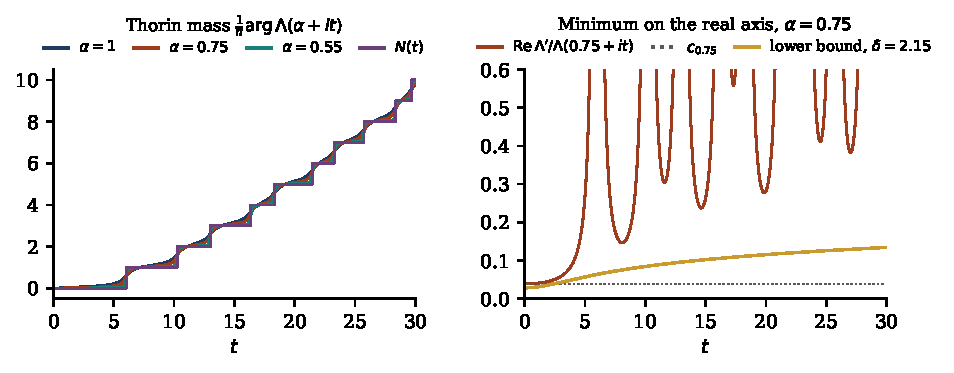
\includegraphics[width=\textwidth]{figs/beta_argument.pdf}
\caption{Left: cumulative Thorin mass $\tau_\alpha((0,t^2])=\pi^{-1}\arg\Lambda(\alpha+it)$ for $\alpha=1,\,0.75,\,0.55$ against the zero counting function $N(t)$ of $\beta$. Right: $\operatorname{Re}\,\Lambda'/\Lambda(0.75+it)$, its value $c_{0.75}$ at $t=0$, and the bound of Corollary~\ref{beta:cor:lower} with $\delta=2.15$, which exceeds $c_{0.75}$ for $t>2.434$.}
\label{beta:fig:arg}
\end{figure}


\section{The centre}\label{beta:sec:centre}

An unconditional input at the centre would be a positive structure of the primal law that does not come from the zeros. One candidate is a scale mixture of $\Gamma(2)$ densities with positive mixing measure, which is infinitely divisible by Kristiansen's theorem \cite{kristiansen1994} (Steutel's conjecture). For $\beta$ neither the two sided nor the one sided form of this holds.

By Remark~\ref{rem:10dnotid}, whose argument is that of Roynette and Yor \cite{roynetteyor2005} for $\xi$, $X_\beta$ is not infinitely divisible: its characteristic function $\Lambda(\tfrac12+it)/\Lambda(\tfrac12)$ vanishes at $t=6.0209489$ (it is $+0.006077$ at $t=5.9$ and $-0.003508$ at $t=6.1$). Nor is $\Lambda(\tfrac12+w)/\Lambda(\tfrac12)$ a positive mixture $\int M(d\lambda)/(w+\lambda)^2$ of $\Gamma(2)$ transforms, since such a mixture decreases on $w>0$ while $\Lambda(\tfrac12+w)$ increases there.

For $\beta$ the one sided object is $\Phi_\beta1_{\{u>0\}}$, whose Laplace transform
\[
\int_0^\infty e^{-wu}\Phi_\beta(u)\,du=\frac12\int_1^\infty x^{(s-1)/2}\eta(ix)^3\,dx,\qquad s=\tfrac12-w,
\]
is an incomplete Mellin transform of $\eta^3$, the analogue of the piece from $x=1$ to $\infty$ in Riemann's theta function proof of the functional equation of $\zeta$ \cite{titchmarsh1986}. It is not a $\Gamma(2)$ mixture either.

\begin{proposition}\label{beta:prop:nocm}
Neither $\Phi_\beta(u)/u$ on $u>0$ nor $\eta(ix)^3$ on $x>0$ is completely monotone; in particular $\Phi_\beta1_{\{u>0\}}$ is not a positive mixture of $\Gamma(2)$ densities.
\end{proposition}

\begin{proof}
A completely monotone $g=\int e^{-\lambda u}M(d\lambda)$ with $M\ne0$ satisfies $g(u)\ge M([0,L])e^{-Lu}$ for any $L$ with $M([0,L])>0$, so it decays at most exponentially, whereas $\Phi_\beta(u)/u$ decays like $\exp(\tfrac32u-\tfrac\pi4e^{2u})$. By \eqref{beta:eq:jacobi} and uniqueness of the Laplace transform, the representing measure of $\eta(ix)^3$ has the signed weights $(-1)^n(2n+1)$ at $\pi(2n+1)^2/4$.
\end{proof}

The decay argument applies to every degree one kernel, since all decay like $\exp(-ce^{2u})$: no P\'olya kernel of a degree one $L$ function, Riemann's kernel $\Phi$ of \eqref{eq:ch10polya} included, is of the form $\int u^{a-1}e^{-\lambda u}M(d\lambda)$ on a half line with $M\ge0$ and $a>0$.

The positivity sits in the reciprocal of the product: with $q=e^{-2\pi x}$ and $\sigma_{-1}(N)=\sum_{d\mid N}d^{-1}$,
\begin{equation}\label{beta:eq:recipprod}
\frac{e^{-\pi x/4}}{\eta(ix)^3}=\prod_{m\ge1}(1-q^m)^{-3}
=\exp\Bigl(3\sum_{N\ge1}\sigma_{-1}(N)\,e^{-2\pi Nx}\Bigr)
\end{equation}
is the exponential of a completely monotone function, hence completely monotone. As in Thorin's theory, the representing measure of $\eta(ix)^3$ is signed while the reciprocal of its product part is the exponential of a positive mixture.


\section{The Dedekind eta function and \texorpdfstring{$\chi_{12}$}{chi 12}}\label{beta:sec:eta}

Euler's pentagonal identity gives $\eta(ix)=\sum_{n\ge1}\chi_{12}(n)e^{-\pi n^2x/12}$, where $\chi_{12}$ is the real even primitive character modulo $12$ with $\chi_{12}(\pm1)=1$ and $\chi_{12}(\pm5)=-1$. As in Section~\ref{beta:sec:primal},
\[
\Lambda_{12}(s):=\Bigl(\frac{12}{\pi}\Bigr)^{s/2}\Gamma\Bigl(\frac s2\Bigr)L(s,\chi_{12})
=\int_0^\infty x^{s/2-1}\eta(ix)\,dx,
\]
so $\Lambda_{12}(\tfrac12+w)=2\int_{\R}e^{wu}\Phi_{12}(u)\,du$ with the even, strictly positive kernel $\Phi_{12}(u)=e^{u/2}\eta(ie^{2u})$, and $\Lambda_{12}(s)=\Lambda_{12}(1-s)$. The L\'evy measure for $\alpha>1$ is $dx/(1-e^{-2x})+\sum_{n\ge2}\chi_{12}(n)\Lambda(n)\delta_{\log n}$, again with positive archimedean and signed prime parts, and with $K=\mathbb Q(\sqrt3)$ one has $\zeta_K=\zeta\cdot L(s,\chi_{12})$.

\begin{theorem}[Real characters; after \cite{polson2018vdp}, Theorem~30 and Remark~32]\label{beta:thm:realchar}
Let $\chi$ be a real primitive character with quadratic field $K$. Then $T^\chi_\alpha(y)=\operatorname{Re}(\Lambda_\chi'/\Lambda_\chi)(\alpha+i\sqrt y)/(2\pi\sqrt y)=T^K_\alpha(y)-T^\xi_\alpha(y)$; by Theorem~\ref{thm:10dshift} the reciprocal $\Lambda_\chi(\alpha)/\Lambda_\chi(\alpha+\sqrt v)$ is a GGC transform for $\alpha\ge1$, and GRH for $\chi$ is equivalent to $T^K_\alpha\ge T^\xi_\alpha$ for every $\alpha>\tfrac12$; and Theorems~\ref{beta:thm:local} and \ref{beta:thm:comp} hold for $\Lambda_\chi$, as does Theorem~\ref{beta:thm:realaxis} when the theta kernel of $\chi$ is positive.
\end{theorem}

\begin{proof}
With $d_K$ the discriminant, put
\begin{align*}
\xi_K(s)&=\tfrac12s(s-1)|d_K|^{s/2}(2\pi)^{-s}\Gamma(s)\zeta_K(s)&&\text{for imaginary $K$},\\
\xi_K(s)&=\tfrac12s(s-1)|d_K|^{s/2}\pi^{-s}\Gamma(\tfrac s2)^2\zeta_K(s)&&\text{for real $K$};
\end{align*}
for $K=\mathbb Q(i)$ the first agrees with the definition above, since $4^{s/2}(2\pi)^{-s}=\pi^{-s}$. Then $\xi_K=c\,\xi\,\Lambda_\chi$ for a constant $c$ (by the duplication formula for imaginary $K$, directly for real $K$); the factor $|d_K|^{s/2}$ is essential, since without it the ratio acquires a factor $e^{ks}$ that shifts $\operatorname{Re}\,\xi_K'/\xi_K$ by a constant. The proofs above then apply to logarithmic derivatives.
\end{proof}

For $\chi_{12}$, $L(\sigma,\chi_{12})$ is $0.125$, $0.334$, $0.499$, $0.625$, $0.721$ at $\sigma=0.1$, $0.3$, $0.5$, $0.7$, $0.9$; the first ordinates are $3.8046$, $6.6922$, $8.8906$, $11.1884$; $V_{12}=0.33292$; the termwise threshold $\alpha_c(\chi_{12})=1.8349$ is the root of
\[
\tfrac12\log\tfrac{12}\pi+\tfrac12\psi(\tfrac\alpha2)=-\frac{\zeta'}\zeta(\alpha)-\frac{\log2}{2^\alpha-1}-\frac{\log3}{3^\alpha-1};
\]
and over $t\in[0,30]$ the minimum of $\operatorname{Re}\,\Lambda_{12}'/\Lambda_{12}(\alpha+it)$ is $c_\alpha$, equal to $0.16508$, $0.08306$, $0.03328$ at $\alpha=1,\,0.75,\,0.6$. The smaller threshold reflects the larger conductor term $\tfrac12\log\frac{12}{\pi}$ and the removal of the primes $2$ and $3$.

\subsection{Open problems}

\begin{problem}[A coupling below $\alpha=1$]\label{op:betacoupling}
Construct the coupling $H^K_\alpha\overset{d}{=}H^\xi_\alpha+H^\beta_\alpha$ of Theorem~\ref{beta:thm:dom} from the Gaussian primes in a form that could survive below $\alpha=1$. By Proposition~\ref{beta:prop:kron} it must use the phases $\chi_{-4}(p)p^{-it}$, not only the sizes of the atoms. A first computation is the smallest margin of $\operatorname{Re}\,\xi_K'/\xi_K-\operatorname{Re}\,\xi'/\xi$ on lines $\tfrac12<\alpha<1$.
\end{problem}

\begin{problem}[Negative windows]\label{op:betawindows}
Find a lower bound for the decrease of $\arg\Lambda(\alpha+it)$ across the window of Theorem~\ref{beta:thm:local} caused by a pair $\tfrac12\pm B+i\gamma$, in terms of $B$, $\alpha$ and the local density of zeros, that a mean value estimate for $\operatorname{Re}\,\Lambda'/\Lambda$ over intervals of length one could contradict.
\end{problem}

\begin{problem}[All lines to the right]\label{op:betalines}
Theorem~\ref{beta:thm:minall}(ii) places the minimum over $t$ of $\operatorname{Re}\,\Lambda'/\Lambda(\alpha+it)$ at $t=0$ for $\tfrac12<\alpha\le3.15$ and $|t|\le H_0-1.2071$. Extend it to every $\alpha>\tfrac12$ at these heights, either by optimising $\delta$ as a function of $\alpha$ or by a direct argument for large $\alpha$, where the prime part is small, and to every height for $\alpha\ge1$. Numerically the minimum over $t\in[0,40]$ is at $t=0$ for $\alpha=1.5,\,2,\,3,\,3.15$ and $5$. For $\xi$ the statement at every height is Lagarias's theorem under RH \cite{lagarias1999}, and unconditionally it is known for $\alpha\ge1$ \cite{garunkstis2002}; the arguments of Lagarias for $\alpha\ge10$, of Garunk\v{s}tis \cite{garunkstis2000,garunkstis2002} and of Broughan \cite{broughan2009} near $\alpha=1$ are natural routes for $\beta$.
\end{problem}

\begin{problem}[Positivity on the reciprocal side]\label{op:betarecip}
By \eqref{beta:eq:recipprod} and its analogue for $\eta$, the functions $e^{-\pi x/4}/\eta(ix)^3$ and $e^{-\pi x/12}/\eta(ix)$ are completely monotone, with representing measures at the points $2\pi n$, $n\ge0$, whose weights are the coefficients of $\prod_m(1-q^m)^{-3}$ and $\prod_m(1-q^m)^{-1}$. Decide whether this positivity passes, through incomplete Mellin transforms, to a positive representation on the reciprocal side of $\Lambda$ or of $\Lambda_{12}$.
\end{problem}


\section{Notes}

The Thorin framework of this chapter is that of Chapters~\ref{ch:10b} and \ref{ch:10d}. For real primitive characters, $\chi_{-4}$ among them, the closed form of the Thorin density, the GGC property for $\alpha>1$ and the equivalence of GRH with the GGC property at every $\alpha>\tfrac12$ are Theorem~30 and Remark~32 of \cite{polson2018vdp}, and Theorem~\ref{thm:10dshift} gives them, with $\alpha\ge1$, for every $L$ function of Chapter~\ref{ch:10b}; Theorems~\ref{beta:thm:thorin}, \ref{beta:thm:uncond} and \ref{beta:thm:grh}, and the corresponding parts of Theorems~\ref{beta:thm:dom} and \ref{beta:thm:realchar}, are their cases; the L\'evy form of Theorem~\ref{beta:thm:levy} is the computation of Section~\ref{sec:10daway} for an odd character. The Mellin form of Proposition~\ref{beta:prop:mellin} is the theta series proof of the functional equation for odd characters \cite{iwanieckowalski2004}, \cite[Section~8.1]{polson2018vdp} relates $\eta^3$ to $\beta$ through its Laplace transform, and Jacobi's identity for $\eta^3$ and Euler's pentagonal identity for $\eta$ are classical. Lemma~\ref{beta:lem:2sin2} is the signed form of Lemma~\ref{lem:10dsin2}, which is Lemma~14 of \cite{polson2018vdp} with a first step of Roynette and Yor \cite{roynetteyor2005}. The splitting $\zeta_K=\zeta\beta$ for $K=\mathbb Q(i)$ is classical, and the induction of the trivial character of $K$ to $1\boxplus\chi_{-4}$ is the simplest case of automorphic induction.

Proposition~\ref{beta:prop:kron} rests on Kronecker's theorem and the linear independence of the $\log p$, as in Proposition~\ref{prop:ch09notcf} and in the value distribution theory of Bohr and Jessen \cite{bohrjessen1930}. For $1<\alpha<\alpha_c\approx2.28$ the atoms of $\beta$ prove positivity only above the height $t_0(\alpha)$, and no bound that uses only their sizes does better; at $\alpha=1$ the nonvanishing of $\beta$ on $\operatorname{Re}s=1$ is what excludes atoms from the Thorin measure, as for $\xi$ in \cite[Remark~21]{polson2018vdp}.

For $\xi$ the minimum of $\operatorname{Re}\,\xi'/\xi$ on the line $\operatorname{Re}s=\alpha$ lies at $t=0$ unconditionally for $\alpha\ge10$ and, under RH, for every $\alpha>\tfrac12$, attained only at $t=0$ (Lagarias \cite{lagarias1999}, Theorems~1.2 and 1.3 and Section~3); Garunk\v{s}tis proved it unconditionally for $\alpha>4.5$ \cite{garunkstis2000} and for every $\alpha\ge1$ \cite{garunkstis2002}, both stated for the infimum, and Lemma~2.5 and Theorem~3.2 of Broughan \cite{broughan2009}, with the verification of RH to height $3\times10^{12}$ \cite{platttrudgian2021}, give the strict inequality for every $t\ne0$ when $\alpha\ge1.043$. The criterion that RH is equivalent to $\operatorname{Re}\,\xi'/\xi>0$ on $\operatorname{Re}s>\tfrac12$ is due to Hinkkanen \cite{hinkkanen1997} and Lagarias \cite{lagarias1999}. In the notation of \eqref{eq:10dU} the minimum at $t=0$ is the positivity of the Thorin density $U$ that remains when the $\tfrac12$ stable part is removed, which \cite[Remark~31]{polson2018vdp} shows can fail for $\Lambda(s,\chi)$ alone with $\chi$ a complex character modulo $5$. As far as we know the following are new in this form: Theorem~\ref{beta:thm:minall} for $\beta$ and its analogue for $\chi_{12}$; for $\xi$, the unconditional range $\tfrac12<\alpha<1$ below height $3\times10^{12}$; and the comparison lemma with its sharp constant $1+\sqrt2$. They are elementary consequences of the Hadamard product, the functional equation and the rigorous verifications of GRH for small conductors by Platt \cite{platt2016} and of RH by Platt and Trudgian \cite{platttrudgian2021}, and none of them proves a Riemann hypothesis. The grouping \eqref{beta:eq:pair} and its consequence, that $\operatorname{Re}\,\xi'/\xi(\sigma+it)$ can be negative only within distance $\tfrac12$ of the ordinate of a zero off the line, are due to Levinson and Montgomery \cite[Section~2]{levinsonmontgomery1974}, and Broughan \cite{broughan2009} uses the same grouping; Corollary~\ref{beta:cor:height} reads them as a localisation of negative Thorin density, a quantitative form of the negative dip noted after Theorem~\ref{thm:10dshift}.

For $\xi$, Theorem~\ref{beta:thm:arg} and Corollary~\ref{beta:cor:argmono} are Theorem~8.2 and part of Theorem~8.4 of \cite{polson2017}. That $X_\beta$ is not infinitely divisible is Remark~\ref{rem:10dnotid}, after Roynette and Yor \cite{roynetteyor2005}. The completely monotone reciprocal product \eqref{beta:eq:recipprod} is a candidate for an unconditional input at the centre on the reciprocal side (Open Problem~\ref{op:betarecip}), not a proof that one exists.

Theorem~\ref{beta:thm:realchar} lists what extends to every real primitive character; the minimum on the real axis, Theorem~\ref{beta:thm:minall}, is established here only for $\chi_{-4}$, $\chi_{12}$ and $\xi$, and Problem~\ref{cp:betareal} asks how far it extends. Problem~\ref{cp:betahecke} poses the same questions for the Hecke characters of $\mathbb Q(i)$, whose $L$ functions are those of $\mathrm{GL}(2)$ newforms with complex multiplication, to which Theorem~\ref{thm:10dshift} already applies.


\section{Exercises}

\begin{enumerate}
\item Prove $\operatorname{Re}\,w/(1-w)\le r/(1-r)$ for $|w|=r<1$, with equality only at $w=r$. Deduce $\operatorname{Re}\,\beta'/\beta(\alpha+it)\ge-S(\alpha)$ for $\alpha>1$, and check $S(2)=-\zeta'/\zeta(2)-\tfrac13\log2=0.339$.
\item Prove Lemma~\ref{beta:lem:comp} from the identity for $g'(w)$ in its proof. Show that $g'(0)>0$ exactly when $(\sqrt2-1)B<|u|<(1+\sqrt2)B$, that $g'(B^2-u^2)>0$ when $0<|u|<B$, and that $Q_B(a,0)/a$ has a pole at $a=B$; conclude that $a\mapsto Q_B(a,u)/a$ is nonincreasing on $a>0$ if and only if $|u|\ge(1+\sqrt2)B$.
\item Show that $x\mapsto a/(a^2+x^2)$ is strictly convex exactly for $|x|>a/\sqrt3$, that $Q_B(a,u)$ is odd in $a$, and that $\partial_u^2Q_B(a,u)=12a\,u^{-4}-40a(a^2+3B^2)u^{-6}+O(u^{-8})$. Where does the proof of Theorem~\ref{beta:thm:minall} use each fact?
\item From Stirling's formula derive the asymptotic of Theorem~\ref{beta:thm:arg} and the constant $\tfrac18$ of the zero counting formula after it. What is the constant for $L(s,\chi_{12})$, whose gamma factor is $\Gamma(\tfrac s2)$?
\item Show that a completely monotone $g=\int e^{-\lambda u}M(d\lambda)$ with $M\ne0$ satisfies $g(u)\ge M([0,L])e^{-Lu}$ whenever $M([0,L])>0$, and deduce that no P\'olya kernel of a degree one $L$ function is a positive mixture of $\Gamma(a)$ densities on a half line, for any $a>0$. Prove \eqref{beta:eq:recipprod}, compute the first five coefficients of $\prod_m(1-q^m)^{-3}$, and explain why the decay argument does not apply to $e^{-\pi x/4}/\eta(ix)^3$.
\item From Jacobi's identity \eqref{beta:eq:jacobi} show that the theta series of $\chi_{-4}$ is $\eta(ix)^3$, and deduce from $\eta(i/x)=\sqrt x\,\eta(ix)$ that $\Phi_\beta$ is even and positive. Do the same for $\Lambda_{12}$ and $\Phi_{12}$ with Euler's pentagonal identity.
\item For a real primitive character $\chi$ with quadratic field $K$ verify $\xi_K=c\,\xi\,\Lambda_\chi$, with $c=1$ for real $K$ and $c=1/(2\sqrt\pi)$ for imaginary $K$, and show that omitting the factor $|d_K|^{s/2}$ changes $\xi_K'/\xi_K$ by the constant $\tfrac12\log|d_K|$. Which statements of this chapter need the theta kernel of $\chi$ to be positive?
\item Show that $\Lambda(1)/\Lambda(1+\sqrt v)$ is a GGC transform, as the weak limit of the transforms at $\alpha\downarrow1$, without using the nonvanishing of $\beta$ on $\operatorname{Re}s=1$, and that a zero of $\beta$ at $1+i\gamma$ would give the Thorin measure at $\alpha=1$ an atom at $\gamma^2$.
\end{enumerate}


\section{Open computational problems}

Each problem can be attacked numerically first, with the closed form \eqref{beta:eq:Tclosed}, the argument form of Theorem~\ref{beta:thm:arg} and the comparison bound of Corollary~\ref{beta:cor:lower}; a sign found numerically is proved only by a computation with error control.

\begin{compproblem}[Minimum on the real axis for real characters]\label{cp:betareal}
Objective: for every real primitive character $\chi$ of conductor at most $10^3$, compute $V_\chi=(\log\Lambda_\chi)''(\tfrac12)$, the termwise threshold $\alpha_c(\chi)$ (for $\chi_{-4}$ and $\chi_{12}$ it is $2.2823$ and $1.8349$) with the heights $t_0(\alpha)$ of Proposition~\ref{beta:prop:kron}, the comparison height $t_1(\chi)$ of Theorem~\ref{beta:thm:minall} for the best $\delta$, and the lowest ordinate $\gamma_1(\chi)$, and record whether the theta kernel of $\chi$ is positive, which Theorem~\ref{beta:thm:realaxis} needs. List the characters with $t_1(\chi)+(\tfrac12+\delta)/\sqrt3\ge\gamma_1(\chi)$, for which the convexity step in the proof of part (ii) fails near the real axis; $\chi_{-163}$ is one, since its lowest ordinate is $0.2029<1/(2\sqrt3)$. Then test whether the minimum over $t$ of $\operatorname{Re}\,\Lambda_\chi'/\Lambda_\chi(\alpha+it)$ is attained at $t=0$ on every line $\tfrac12<\alpha\le10$. Objects and scale: the real primitive characters of conductor at most $10^3$, about six hundred; $\alpha$ on a grid of step $0.01$; $|t|\le100$. Route: PARI/GP (\texttt{lfuninit}, \texttt{lfunlambda}, \texttt{lfunzeros}) for $\Lambda_\chi$, its logarithmic derivative and its zeros, with the number of zeros checked by the argument principle; $\alpha_c(\chi)$ by root finding as in Section~\ref{beta:sec:eta}; ball arithmetic to prove the signs near the minima and for the characters near the failure boundary. Deliverable: a table by conductor and parity of $V_\chi$, $\alpha_c(\chi)$, $t_1(\chi)$, $\gamma_1(\chi)$, the sign of the kernel and the smallest margin over $t$ on each line; the exceptional characters, with a separate argument for part (ii) where one can be found; and fits of $V_\chi$, $\gamma_1(\chi)$ and $\alpha_c(\chi)$ against $\log q$. Why it matters: it shows how far Theorem~\ref{beta:thm:minall}, the analogue for $\beta$ of Lagarias's theorem \cite{lagarias1999}, reaches among real characters as the conductor grows and the lowest zero comes down, on average, towards the real axis; only the signs proved in ball arithmetic are verified.
\end{compproblem}

\begin{compproblem}[Hecke characters of the Gaussian field]\label{cp:betahecke}
Objective: for the Hecke characters \cite{hecke1918} $\lambda_k((a))=(a/|a|)^{4k}$ of $\mathbb Q(i)$, whose $L$ functions are those of the newforms with complex multiplication of weight $4k+1$ and level $4$, compute on lines $\alpha>\tfrac12$ the Thorin density of Theorem~\ref{thm:10dshift}, the termwise threshold $\alpha_c(\lambda_k)$ and the analogue of Proposition~\ref{beta:prop:kron}, the constants $V$ and $t_1$ and the first ordinate, and test the minimum on the real axis of Theorem~\ref{beta:thm:minall}, after checking the root number and the sign of the P\'olya kernel. Objects and scale: $k=1,\dots,5$, weights $5$ to $21$; ordinates to height $10^3$. Route: PARI/GP \texttt{mfinit} and \texttt{lfuncreate} for the newforms, or \texttt{gcharinit} for the characters, with \texttt{lfunzeros}; archimedean factor $\Gamma_{\mathbb C}(s+2k)$ in the unitary normalisation; atoms $2\cos(4km\theta_p)\log p$ at $p^m$ for split $p=\pi\bar\pi$ with $\theta_p=\arg\pi$, $2\log p$ at the even powers of inert $p$, and $(-1)^{km}\log2$ at $2^m$; ball arithmetic near the minima. Deliverable: for each $k$ the threshold, $V$, $t_1$, the first ordinate and the minimum of $\operatorname{Re}\,\Lambda'/\Lambda(\alpha+it)-c_\alpha$ for $\alpha\in\{0.6,0.75,1\}$ over the scanned range, with the lines on which the minimum leaves the real axis, compared with the real characters of Problem~\ref{cp:betareal}. Why it matters: the atoms are cosines of the angles of Gaussian primes rather than signs, so Kronecker's theorem acts on angles, and the problem tests whether the minimum on the real axis is special to Dirichlet characters.
\end{compproblem}

\begin{compproblem}[Synthetic off line zeros]\label{cp:betasynthetic}
Objective: insert a hypothetical pair $\tfrac12\pm B+i\gamma$, with its conjugates, into the true zeros of $\beta$ and measure (a) the decrease of $\arg\Lambda(\alpha+it)$ across the window of Theorem~\ref{beta:thm:local}; (b) the distance from the off line ordinate beyond which complete monotonicity in the width survives: under GRH, $(\alpha-\tfrac12)^{-1}\operatorname{Re}\,\Lambda'/\Lambda(\alpha+it)=\sum_{\gamma'}1/(w+(t-\gamma')^2)$ over the true ordinates $\gamma'$, with $w=(\alpha-\tfrac12)^2$, is a Stieltjes function of $w$ with representing function $\rho_t(x)=\sum_{\gamma'}e^{-x(t-\gamma')^2}$, while the pair adds $2e^{-cx}\cos\kappa x$ with $u=t-\gamma$, $c=u^2-B^2$ and $\kappa=2|u|B$, which changes sign, so the distance is the analogue of the constant $1+\sqrt2$ of Lemma~\ref{beta:lem:comp}; and (c) the depth of the negative lobe of the signed density $u_\varepsilon$ of Proposition~\ref{prop:scholzelobe} (whose $A$ and $B$ are $\gamma^2-B^2$ and $2\gamma B$ in the notation here), and whether the neighbouring zeros mask it. Objects and scale: $L(s,\chi_{-4})$, its zeros to height $10^3$, $B$ from $10^{-3}$ to $0.4$, ten values of $\gamma$, lines $\tfrac12<\alpha\le1$. Route: the true $\Lambda$ from PARI/GP \texttt{lfunlambda} times the Hadamard factors of the synthetic zeros; the closed forms of Theorem~\ref{beta:thm:arg} and Lemma~\ref{beta:lem:comp}; $\rho_t(x)$ on a logarithmic grid $10^{-4}\le x\le10^4$, with the tail of the zero sum bounded through the zero counting formula; ball arithmetic wherever a sign is claimed. Deliverable: the three quantities as functions of $B$, $\alpha$ (or $\varepsilon$) and the local density of zeros, and the smallest $B$ detected at each $\varepsilon$. Why it matters: it measures how visible a zero off the line is in the Thorin measure, in its argument and in the signed densities of Chapter~\ref{ch:scholze}, which is what Open Problems~\ref{op:betawindows} and \ref{op:scholzelobe} ask to turn into bounds; an experiment with synthetic zeros proves nothing about the true ones.
\end{compproblem}

\chapter[Signed Thorin Measures]{Signed Thorin Measures and the Argument Principle}\label{ch:scholze}

By Theorem~\ref{thm:10bmain}, the generalized Riemann hypothesis (GRH) for an automorphic $L$ function holds if and only if its Thorin measure, with unit atoms at the squared ordinates $\gamma_k^2$ of its zeros, is a positive measure on $(0,\infty)$. This chapter computes a smoothed signed version of that measure, with no hypothesis on the zeros, by Stieltjes inversion of the logarithmic derivative of the clock $\Lambda(c+\sqrt s)/\Lambda(c)$ at distance $\varepsilon$ above its cut; positivity of the resulting density $u_\varepsilon$ for every $\varepsilon$, together with the absence of real zeros, which $u_\varepsilon$ does not see, is the Herglotz criterion of Theorem~\ref{thm:10bmain}(e). We compute $u_\varepsilon$ for $\zeta$, $L(s,\chi_{12})$ and $L(s,\Delta)$, show how an off line pair of zeros appears in it and why one value of $\varepsilon$ cannot exclude such a pair, and count zeros by the argument principle, which sees every zero at once. Such a positivity statement contains GRH and is not evidence for it; a finite computation tests it to a height, and none below is certified, since none has error control.

\section{Where Scholze's work enters}\label{sec:scholzegalois}

The $L$ functions of this chapter are classical. For a cuspidal automorphic representation $\pi$ of $\GL_n$ over $\Q$, the completed function $\Lambda(s,\pi)$, its continuation to an entire function of order one and its functional equation are due to Godement and Jacquet \cite{godementjacquet1972}, after Hecke and Tate for $n=1$ \cite{hecke1918,tate1967} and Hecke for modular forms \cite{hecke1936,hecke1937}; the conductor is that of Jacquet, Piatetski Shapiro and Shalika \cite{jpss1981}. The archimedean factor is determined by the component $\pi_\infty$ through Langlands's archimedean correspondence \cite{langlands1989,knapp1994}; for the $L$ function of a motive it is fixed by the Hodge numbers and the action of complex conjugation \cite{serre1970}.

Scholze's work enters on the Galois side. He attached Galois representations to torsion classes in the cohomology of the locally symmetric spaces of $\GL_n$ over totally real and CM fields \cite{scholze2015}, and gave a new proof \cite{scholze2013} of the local Langlands correspondence for $\GL_n$ of Harris and Taylor and of Henniart \cite{harristaylor2001,henniart2000}. The torsion representations feed the potential automorphy theorems of Allen, Calegari, Caraiani, Gee, Helm, Le Hung, Newton, Scholze, Taylor and Thorne \cite{allen2023}: for an elliptic curve over a CM field, and more generally for a rank two compatible system of weight zero, every symmetric power $L$ function has meromorphic continuation to $\C$ and a functional equation (Corollary~7.1.13 there). A meromorphic continuation does not give the entire completed function that Theorem~\ref{thm:10bmain} needs, and a torsion class has no complex $L$ function at all. Fargues and Scholze \cite{farguesscholze2026} attach to every irreducible smooth representation of a reductive group over a nonarchimedean local field a semisimple $L$ parameter; for $\GL_n$ it is the semisimplification of the parameter of the local correspondence, and it does not determine the local $L$ and $\varepsilon$ factors (the trivial and the Steinberg representations of $\GL_2(\Q_p)$ share one).

None of this enters the computations below, nor does Deligne's Galois representation of $\Delta$ \cite{deligne1971}. What the Galois side supplies is new $L$ functions: once a representation of $\operatorname{Gal}(\overline{\Q}/\Q)$ is shown to be cuspidal automorphic, its $L$ function falls under Theorem~\ref{thm:10bmain} and the methods of this chapter.

\section{The signed density of a clock}\label{sec:scholzesigned}

Let $\pi$ be self dual, $\pi\cong\tilde\pi$, with $\Lambda(s,\pi)$ completed as in Section~\ref{sec:10bcompletion}, the conductor factor $N_\pi^{s/2}$ included; here $c=\frac12$, except that for $\Delta$ we keep the classical normalisation of Chapter~\ref{ch:10}, with centre $c=6$. Let $r$ be the order of $\Lambda(s,\pi)$ at $s=c$ and $\Xi^{\mathrm{sd}}_\pi(z)=\Lambda(c+z,\pi)/z^r$ as in Definition~\ref{def:10bxi} (for $\Delta$ the definition carries a factor $2$, which cancels in $G_\pi$); it is even, since $\varepsilon(\pi)=(-1)^r$ (Lemma~\ref{lem:10bcompletion}(v)). The \emph{clock}\index{clock} of $\pi$ is
\[
G_\pi(s)=\frac{\Xi^{\mathrm{sd}}_\pi(\sqrt s)}{\Xi^{\mathrm{sd}}_\pi(0)},
\]
an entire function of order at most $\frac12$ with $G_\pi(0)=1$ and $G_\pi^2=F_\pi$; for $\zeta$, with $\Lambda=\xi$, it is $F_\zeta$ itself. The three $L$ functions of this chapter have root number $+1$ and $\Lambda(c,\pi)\ne0$, so $r=0$ and $G_\pi(s)=\Lambda(c+\sqrt s,\pi)/\Lambda(c,\pi)$; we assume $r=0$ from now on.

List the zeros of $\Xi^{\mathrm{sd}}_\pi$ in pairs $\pm i\gamma_k$ with multiplicity and put $t_k=\gamma_k^2$, as in \eqref{eq:10batoms}. Then $G_\pi(s)=\prod_k(1+s/t_k)$ and
\begin{equation}\label{eq:scholzelog}
\frac{G_\pi'}{G_\pi}(s)=\sum_k\frac1{s+t_k}=\frac1{2\sqrt s}\,\frac{\Lambda'}{\Lambda}(c+\sqrt s,\pi).
\end{equation}
Every zero $c+\delta+i\gamma$ of $\Lambda(s,\pi)$ has $|\delta|<\frac12$ (Lemma~\ref{lem:10bcompletion}(iii)). A zero on the line, $\delta=0<\gamma$, gives the atom $\gamma^2>0$; a zero with $\gamma>0$ and $\delta\ne0$, with its reflection $c-\delta+i\gamma$, gives the conjugate atoms $A\pm iB$, where $A=\gamma^2-\delta^2$ and $B=2\gamma|\delta|$; and a real zero $c\pm\beta$ gives the atom $-\beta^2$. By Theorem~\ref{thm:10bmain}, with $\Xi^{\mathrm{sd}}_\pi$ for $\Xi_\pi$, GRH for $\pi$ holds if and only if $1/G_\pi$ is the Laplace transform of a generalized gamma convolution (Definition~\ref{def:ch10ggc}); its Thorin measure is then $\tau_\pi=\sum_k\delta_{t_k}$, and $(G_\pi'/G_\pi)(s)=\int\tau_\pi(dt)/(s+t)$.

For $\varepsilon>0$ and real $z$ the \emph{signed density}\index{signed Thorin density} of $\pi$ is
\[
u_\varepsilon(z)=-\frac1\pi\operatorname{Im}\frac{G_\pi'}{G_\pi}(-z+i\varepsilon).
\]
By \eqref{eq:scholzelog} it is computed from $\Lambda'/\Lambda$ alone, at points to the right of the critical line, and needs no hypothesis. Under GRH it is the Lorentzian smoothing of $\tau_\pi$ at width $\varepsilon$, which tends to $\tau_\pi$ as $\varepsilon\to0$ (Stieltjes inversion\index{Stieltjes inversion} \cite{akhiezer1965}). The condition $u_\varepsilon\ge0$ for all $\varepsilon>0$ and real $z$ says $\operatorname{Im}(G_\pi'/G_\pi)\le0$ on the upper half plane: it is the inequality of the Herglotz criterion of Theorem~\ref{thm:10bmain}(e), with $G_\pi$ for $F_\pi$, read on the lines $\operatorname{Im}s=\varepsilon$ (Problem~14.2 maps it on a grid); the criterion also excludes real zeros, which give positive Lorentzians (Proposition~\ref{prop:scholzelobe}(iii)). Write $\sqrt{-z+i\varepsilon}=a+iy$ with $a,y>0$, so that $z=y^2-a^2$ and $\varepsilon=2ay$, and let $L=(\Lambda'/\Lambda)(c+a+iy,\pi)$. Then
\[
u_\varepsilon(z)=\frac{y\operatorname{Re}L-a\operatorname{Im}L}{2\pi(a^2+y^2)},\qquad V_a(y^2)=\frac{\operatorname{Re}L}{2\pi y},
\]
where $V_a$ is the density of Theorem~\ref{thm:10dshift}, formed with $\Xi^{\mathrm{sd}}_\pi$ for $\Xi_\pi$. So $u_\varepsilon$ and $V_a$ read $\Lambda'/\Lambda$ on the same vertical line, at distance $a=\varepsilon/(2y)$ to the right of the centre; $u_\varepsilon$ adds the term in $\operatorname{Im}L$ and the factor $y^2/(a^2+y^2)$. At $z=A$ the threshold $\varepsilon=B$ of the next proposition is the point $a+iy=|\delta|+i\gamma$, the condition $|\operatorname{Re}z_k|=a$ of Theorem~\ref{thm:10dshift}, and the lobe is the dip of $V_a$ described after it.

\begin{proposition}[The negative lobe]\label{prop:scholzelobe}\index{negative lobe}
Let $\pi$ be as above, with $r=0$, and $\varepsilon>0$.
\begin{enumerate}
\item[(i)] A zero $c+i\gamma$, $\gamma>0$, of multiplicity $m$ contributes to $u_\varepsilon$ the Lorentzian $\frac m\pi\,\varepsilon/((z-\gamma^2)^2+\varepsilon^2)$, of mass $m$ and height $m/(\pi\varepsilon)$, centred at $\gamma^2$.
\item[(ii)] A zero $c+\delta+i\gamma$ with $\gamma>0$ and $\delta\ne0$, together with its reflection, contributes
\[
\frac1\pi\,\frac{B+\varepsilon}{(z-A)^2+(B+\varepsilon)^2}-\frac1\pi\,\frac{B-\varepsilon}{(z-A)^2+(B-\varepsilon)^2}.
\]
For $\varepsilon<B$ this is negative exactly on $|z-A|<(B^2-\varepsilon^2)^{1/2}$ and equals $-2\varepsilon/(\pi(B^2-\varepsilon^2))$ at $z=A$; its integral over $z$ is $0$, and its absolute value is at most $2\varepsilon/(\pi(B-\varepsilon)^2)$.
\item[(iii)] A real zero $c\pm\beta$, $0<\beta<\frac12$, contributes a Lorentzian centred at $-\beta^2$, positive at every $z$.
\item[(iv)] If $\Lambda(\sigma,\pi)\ne0$ for every real $\sigma$, then $u_\varepsilon(z)\ge0$ for all real $z$ and all $\varepsilon>0$ (away from the poles of $G_\pi'/G_\pi$) if and only if every zero lies on the line. If moreover no zero has ordinate in $(0,\frac12]$, the same holds with $z$ restricted to $(0,\infty)$.
\end{enumerate}
\end{proposition}

\begin{proof}
An atom $t=A'+iB'$ contributes $-\pi^{-1}\operatorname{Im}(-z+i\varepsilon+t)^{-1}=\pi^{-1}(B'+\varepsilon)/((z-A')^2+(B'+\varepsilon)^2)$, a Lorentzian centred at $A'$ of mass $\operatorname{sign}(B'+\varepsilon)$; with $B'=0$ this gives (i) and (iii). In (ii) put $x=z-A$ and $f(b)=b/(x^2+b^2)$, so that the pair contributes $\pi^{-1}(f(b_1)-f(b_2))$ with $b_1=B+\varepsilon$ and $b_2=B-\varepsilon$. Since $f(b_1)-f(b_2)=(b_1-b_2)(x^2-b_1b_2)/((x^2+b_1^2)(x^2+b_2^2))$, it has the sign of $x^2-(B^2-\varepsilon^2)$; its value at $x=0$ is $\pi^{-1}(1/b_1-1/b_2)$, its two terms have masses $1$ and $-1$, and $|f'(b)|\le b^{-2}$ with the mean value theorem gives the bound. In (iv), if every zero is on the line every term is positive. Conversely let $c+\delta+i\gamma$ be a zero of multiplicity $m$ with $\delta\ne0$; by hypothesis $\gamma\ne0$, and we may take $\gamma>0$. As $\varepsilon\uparrow B$ its pair contributes $-2m\varepsilon/(\pi(B^2-\varepsilon^2))\to-\infty$ at $z=A$, while the other terms stay bounded near $(z,\varepsilon)=(A,B)$: a term is unbounded there only if its atom is $A-iB$, and the series converges uniformly there because $\sum_k|t_k|^{-1}<\infty$. So $u_\varepsilon(A)<0$ for $\varepsilon$ close to $B$. If no ordinate lies in $(0,\frac12]$, then $\gamma>\frac12>|\delta|$ and $A>0$.
\end{proof}

At a fixed $\varepsilon$ the sign of $u_\varepsilon$ excludes nothing by itself. A pair with $B<\varepsilon$ contributes two positive Lorentzians, and a pair with $B>\varepsilon$ shows only if the other atoms contribute less than $2\varepsilon/(\pi(B^2-\varepsilon^2))$ near $z=A$. An atom on the line at $A$ adds $1/(\pi\varepsilon)$ there, and for $B=3\varepsilon$ the three Lorentzians sum to
\[
\frac{3\varepsilon(x^4+2\varepsilon^2x^2+16\varepsilon^4)}{\pi(x^2+16\varepsilon^2)(x^2+4\varepsilon^2)(x^2+\varepsilon^2)}>0,\qquad x=z-A,
\]
so the pair is masked (Open Problem~\ref{op:scholzelobe}). By (ii) the contribution of each off line pair tends to $0$ as $\varepsilon\to0$: in the limit $u_\varepsilon$ sees only the real atoms, whether or not GRH holds, and off line zeros are seen only at positive $\varepsilon$.

\section{Three clocks}\label{sec:scholzeclocks}

The computations use $\zeta$ with $\Lambda=\xi$; $L(s,\chi_{12})$, where $\chi_{12}$ is the even real character of $\Q(\sqrt3)$, with $\Lambda(s,\chi_{12})=(12/\pi)^{s/2}\Gamma(s/2)L(s,\chi_{12})$; and $L(s,\Delta)$, with $\Lambda(s,\Delta)=(2\pi)^{-s}\Gamma(s)L(s,\Delta)$ and $c=6$. Their P\'olya kernels are positive: P\'olya's kernel \eqref{eq:ch10polya}; the kernel $\Phi_{12}(u)=e^{u/2}\eta(ie^{2u})$ of Section~\ref{beta:sec:eta}, built from $\eta$, the theta function of $\chi_{12}$ by Euler's pentagonal identity; and $\Delta(ie^u)e^{6u}$ (Proposition~\ref{prop:ch10mellin}). So $\Lambda(c+x,\pi)$, a positive multiple of $\int\Phi(u)e^{xu}\,du$, is positive for real $x$, the hypothesis of Proposition~\ref{prop:scholzelobe}(iv) holds, and the lowest ordinates, $14.13$, $3.80$ and $9.22$, exceed $\frac12$.

Positivity of the kernel holds for $\zeta$, $\Delta$ and every multiplicative eta product (the paragraph after Lemma~\ref{lem:10bkernel}) and for $\chi_{-4}$ and $\chi_{12}$ (Chapter~\ref{ch:beta}), but not in general. For the even real character $\chi$ of conductor $53$ the kernel is negative at $u=0$, since $\sum_{n\ge1}\chi(n)e^{-\pi n^2/53}=-0.111$, and infinitely many even real characters have a theta function with a positive real zero \cite{louboutinmunsch2013}; the kernels of infinitely many imaginary quadratic fields change sign (Theorem~\ref{thm:sf:inert}); and for the eigenform $f$ of weight $24$ and level one with $a(2)=540-12\sqrt{144169}$, whose root number is $+1$, the kernel $f(ie^u)e^{12u}$ is negative at $u=0$, where $f(i)=-0.0095$. Open Problem~\ref{op:scholzekernel} asks which kernels are positive.

We computed $u_2$ on a grid in $z$ with mpmath at twenty digits: for $\zeta$ from the logarithmic derivative of $\xi$, for $\chi_{12}$ from the Hurwitz zeta functions $\zeta(s,b/12)$, and for $\Delta$ from Hecke's integral of Proposition~\ref{prop:ch10mellin}, folded at $y=1$, and its derivative \cite{hecke1936}, with grid steps $0.875$ for $T=35$ and $1$ for $\Delta$ with $T=30$. Independently, sign changes of $t\mapsto\Lambda(c+it,\pi)$, refined by bisection, located the zeros on the line (Table~\ref{tab:scholzescan}).

\begin{table}[ht]
\centering
\caption{Zeros on the line below height $T$, and the minimum and mass of $u_2$ on $(0,T^2]$ (numerical, not certified).}\label{tab:scholzescan}
\begin{tabular}{lcccc}
clock & $T$ & zeros on the line & $\min u_2$ & mass of $u_2$\\[2pt]
$\zeta$, $c=\frac12$ & $35$ & $5$ & $2.4\cdot10^{-5}$ & $4.99$\\
$L(s,\chi_{12})$, $c=\frac12$ & $35$ & $17$ & $4.0\cdot10^{-4}$ & $17.2$\\
$L(s,\Delta)$, $c=6$ & $30$ & $8$ & $1.3\cdot10^{-4}$ & $7.98$
\end{tabular}
\end{table}

On each range $u_2$ is positive. For $\zeta$ and $\Delta$ its minimum sits at the first grid point, since $u_2$ increases on $(0,t_1)$; for $\chi_{12}$ it is the trough at $z=1158.5$ between the last atom below $35^2$ and the first above. Every sampled peak lies within six per cent of $1/(2\pi)=0.159$ and within half a grid step of an atom. The excess mass $17.2$ for $\chi_{12}$ is leakage from the Lorentzians of the atoms above $35^2$, mostly that of the zero at $35.027$, and shrinks with $\varepsilon$ (the mass is $17.14$ at $\varepsilon=1$). The ordinates found, whose squares are the atoms of $\tau_\zeta$, $\tau_{\chi_{12}}$ and $\tau_\Delta$, agree with PARI/GP \cite{pari2023} to $10^{-13}$; the first of them are
\[
\begin{aligned}
\tau_\zeta:\;& 14.134725,\ 21.022040,\ 25.010858,\ 30.424876,\ 32.935062, \\
\tau_{\chi_{12}}:\;& 3.804628,\ 6.692223,\ 8.890593,\ 11.188393,\ 12.966179,\ \dots \\
\tau_\Delta:\;& 9.222379,\ 13.907550,\ 17.442777,\ 19.656513,\\
& 22.336104,\ 25.274637,\ 26.804391,\ 28.831683 .
\end{aligned}
\]

To see the lobe of Proposition~\ref{prop:scholzelobe}(ii), take the first five atoms of $\tau_\zeta$ and move the third zero off the line by $\delta=0.3$, so that $A=625.45$ and $B=15.01$. At $\varepsilon=2$ the signed density of this toy clock has a negative lobe of depth $-5.7\cdot10^{-3}$ centred at $z=A$, close to the value $-2\varepsilon/(\pi(B^2-\varepsilon^2))$ of the pair alone, and at $\varepsilon=20>B$ the lobe is gone. The test fires on this isolated pair; by the masking example it need not fire on a pair with an atom on the line near $A$.

For $\zeta$ the total variation distance on $(0,35^2]$ between $u_\varepsilon$ and the Lorentzian smoothing of the five atoms below $35^2$ is $0.0062$, $0.0031$ and $0.0015$ at $\varepsilon=2$, $1$ and $\frac12$. It is the leakage into the window of the atoms $t_k>T^2$, since those below contribute equally to both,
\begin{align*}
&\frac1\pi\sum_{t_k>T^2}\Bigl[\arctan\frac{t_k}\varepsilon-\arctan\frac{t_k-T^2}\varepsilon\Bigr]\\
&\qquad=\frac\varepsilon\pi\sum_{t_k>T^2}\Bigl[\frac1{t_k-T^2}-\frac1{t_k}\Bigr]+O(\varepsilon^3),
\end{align*}
which for $\zeta$ at $T=35$ is $0.00619$, $0.00310$ and $0.00155$. So the two measures agree as $\varepsilon\to0$, as they must once every zero below height $35$ is on the line. The largest sampled values, $0.3175$ at $\varepsilon=1$ and $0.6300$ at $\varepsilon=\frac12$, are within about one per cent of $1/(\pi\varepsilon)$, so no peak carries a double atom.

\section{Zero counts by the argument principle}\label{sec:scholzewinding}

The smoothed mass only approximates a count, and by Proposition~\ref{prop:scholzelobe} one value of $\varepsilon$ can miss an off line pair; the argument principle\index{argument principle} sees every zero. Suppose that $\Lambda(s,\pi)$ has no real zero, and let $N_\pi(T)$ be the number of zeros $c+\delta+i\gamma$ with $0<\gamma\le T$, on the line or not, counted with multiplicity. For $a>\frac12$ and $T$ not an ordinate these are the zeros inside the rectangle $R=c+[-a,a]\times i[0,T]$, and
\[
N_\pi(T)=\frac1{2\pi}\operatorname{var}_{\partial R}\arg\Lambda(s,\pi),
\]
the change of $\arg\Lambda$ around $\partial R$ divided by $2\pi$, which needs no derivative. Computed from samples, it is guaranteed to be right if $\arg\Lambda$ moves by less than $\pi$ between consecutive samples: the phase steps, each reduced to $(-\pi,\pi]$, add up around a closed contour to $2\pi$ times an integer whatever the sampling, so an integer output is no check by itself. If $N_\pi(T)$ equals the number of sign changes of the real function $t\mapsto\Lambda(c+it,\pi)$ on $(0,T]$, every zero of height at most $T$ is on the line and simple. Table~\ref{tab:scholzewinding} gives the counts for $a=0.9$.

\begin{table}[ht]
\centering
\caption{Sign changes of $\Lambda(c+it)$ on $(0,T]$ and winding numbers of $\Lambda$ around $\partial R$, from $400$ samples per side at twelve digits (numerical, not certified).}\label{tab:scholzewinding}
\begin{tabular}{lccc}
clock & $T$ & sign changes of $\Lambda(c+it)$ & winding number\\[2pt]
$\zeta$ & $35$ & $5$ & $5$\\
$\zeta$ & $200$ & $79$ & $79$\\
$L(s,\chi_{12})$ & $35$ & $17$ & $17$\\
$L(s,\chi_{12})$ & $100$ & $67$ & $67$\\
$L(s,\Delta)$ & $30$ & $8$ & $8$
\end{tabular}
\end{table}

In every row the two counts agree, and the largest phase step between samples is $0.39\pi$, for $\zeta$ at $T=200$. With $100$, $50$ and $25$ samples per side the same code returns the integers $35$, $-5$ and $-1$ there. So, numerically, every zero of $\zeta$ below height $200$, of $L(s,\chi_{12})$ below $100$ and of $L(s,\Delta)$ below $30$ is on the line and simple. This is not a certificate, which would need interval arithmetic with a bound for $|\Lambda'/\Lambda|$ on each side (Problem~\ref{cp:scholzewinding}) or Turing's method \cite{turing1953,booker2006}. That these zeros lie on the line is known: Backlund reported that the $79$ zeros of $\zeta$ below height $200$ lie on the line \cite{backlund1914}, a statement contained in later verifications \cite{platttrudgian2021}, Rumely verified GRH for the primitive characters of conductor at most $13$ to height $10^4$ \cite{rumely1993}, and Hiary, Ireland and Kyi verified that every zero of $L(s,\Delta)$ up to height $84$ is on the line \cite[Section~7.3]{hik2027}. The counts agree with the main terms of the Riemann von Mangoldt formula and its analogues \cite{titchmarsh1986,iwanieckowalski2004}: $79.19$, $67.55$ and $7.97$ for $T=200$, $100$ and $30$.

The $\Delta$ row needs care. On the line $|\Lambda(6+it,\Delta)|$ carries the factor $t^{11/2}e^{-\pi t/2}$ and falls to $5\cdot10^{-17}$ at $t=30$ and $2.6\cdot10^{-36}$ at $t=60$, against an integrand of size $10^{-3}$ in Hecke's integral; at twelve digits about two correct digits remain at $t=30$ and none from $t=35$ on. The winding number is still $8$, but the zero search is not reliable: at twelve digits, grids of $100$ to $400$ points on $(0,30]$ find $8$ sign changes and grids of $600$ to $1200$ points find two spurious ones between the zeros at $25.27$ and $26.80$. The grid of the run in the table is not recorded; the eight ordinates of $\tau_\Delta$ come from the run at twenty digits, where each of seventeen grids of $100$ to $3000$ points gives them. At fifty digits one evaluation at $t=60$ takes about $0.57$ seconds, about $15$ minutes for a contour of $1600$ points. Beyond $T\approx30$ the clock of $\Delta$ is better computed from the Ramanujan coefficients through a smoothed approximate functional equation, with about $t/(2\pi)$ terms at height $t$, for instance as in Rubinstein's method \cite[Section~3.3]{rubinstein2005}, where a factor $w^{-s}$ with $|w|=1$ offsets the exponential decay of the gamma factor; Problem~13.1 asks for the zeros of $\Lambda(6+it,\Delta)$ to height $10^5$, with the count certified by Turing's method.

\subsection{Open problems}

\begin{problem}[Positive P\'olya kernels]\label{op:scholzekernel}
Characterise the self dual $L$ functions with root number $+1$ whose P\'olya kernel is positive (Section~\ref{sec:scholzeclocks}); for a form of level one, positivity fails as soon as the form has a zero of odd order on the imaginary axis. Is positivity, at fixed degree, decided by finitely many coefficients and the conductor?
\end{problem}

\begin{problem}[Masking of the negative lobe]\label{op:scholzelobe}
Find conditions on the zeros near height $\gamma$ under which $u_\varepsilon\ge0$ at one $\varepsilon$ excludes a zero $c+\delta+i\gamma$ with $2\gamma|\delta|>\varepsilon$; equivalently, compare the depth $2\varepsilon/(\pi(B^2-\varepsilon^2))$ of the lobe of an off line pair with the contribution of the neighbouring atoms near $z=A$ (compare the dip of $V_a$ after Theorem~\ref{thm:10dshift}).
\end{problem}

\section{Notes}

Theorem~\ref{thm:10bmain} extends \cite{polson2018vdp}, and the densities $V_a$ of Theorem~\ref{thm:10dshift} are, for $\xi$, its Theorem~18; Stieltjes inversion is classical \cite{stieltjes1894,akhiezer1965}. Proposition~\ref{prop:scholzelobe}, the masking identity and the leakage formula are elementary consequences of \eqref{eq:scholzelog}; for $\xi$ the Poisson kernel smoothing of the ordinates and its limit are in \cite{polson2018vdp}, and \cite{polson2026thorin} shows that pointwise positivity of the Thorin density of $\xi(\sigma)/\xi(\sigma+s)$ forces every extremal zero onto the critical line, with an explicit negative value of the density when the first zero is off the line. The computations of Sections~\ref{sec:scholzeclocks} and~\ref{sec:scholzewinding} were made for this book. P\'olya's kernel is in \cite{polya1926}, the kernel of $\chi_{12}$ comes from $\eta$ through Euler's pentagonal identity (Section~\ref{beta:sec:eta}), and that of $\Delta$ is Hecke's Mellin transform \cite{hecke1936}; the values for the character of conductor $53$ and the eigenform of weight $24$ were computed for this book. RH and GRH are verified far beyond the heights of Table~\ref{tab:scholzewinding} for $\zeta$ and $\chi_{12}$ \cite{platttrudgian2021,platt2016}, and for $\Delta$ to height $84$ \cite{hik2027}; Turing's method is in \cite{turing1953}, and its extension to other $L$ functions in \cite{booker2006}. The scripts are in \texttt{scholze/} (Appendix~\ref{app:B}); PARI/GP \cite{pari2023} gave independent zero lists and values.

\section{Exercises}

\begin{enumerate}
\item Derive the formulas for $u_\varepsilon(z)$ and $V_a(y^2)$ in Section~\ref{sec:scholzesigned}, and show that $u_\varepsilon(z)-V_a(y^2)=-a(a\operatorname{Re}L+y\operatorname{Im}L)/(2\pi y(a^2+y^2))$.
\item Add an atom on the line at $A$ to the pair of Proposition~\ref{prop:scholzelobe}(ii), and show that the sum is negative at $z=A$ if and only if $B/\sqrt3<\varepsilon<B$. Verify the masking identity for $B=3\varepsilon$.
\item Derive the closed form of the leakage in Section~\ref{sec:scholzeclocks}, and show that its expansion in $\varepsilon$ has no term of order $\varepsilon^2$.
\item Let $\Lambda$ be holomorphic and zero free near a closed polygon $P$, with $|\Lambda'/\Lambda|\le M$ on $P$. Show that sampled phase differences, reduced to $(-\pi,\pi]$, add up to $2\pi$ times an integer, and that this integer is the winding number of $\Lambda$ around $P$ when consecutive samples are less than $\pi/M$ apart along $P$.
\item Let $f$ be the eigenform of weight $18$ and level one. From $f(-1/\tau)=\tau^{18}f(\tau)$ show that $f(i)=0$, that the kernel $f(ie^u)e^{9u}$ is odd, and that $\Lambda(9+z,f)/z$ is even.
\end{enumerate}

\section{Open computational problems}

\begin{compproblem}[Signs of P\'olya kernels across degrees]\label{cp:scholzekernel}
Objective: decide for self dual $L$ functions of degree at most four with root number $+1$ whether the P\'olya kernel of $\Xi^{\mathrm{sd}}_\pi$ (Lemma~\ref{lem:10bkernel}) is positive, and where it first changes sign. Objects and scale: the $L$ functions of degree at most $4$ and conductor at most $10^3$ in the LMFDB \cite{lmfdb} (newforms, symmetric squares, Rankin Selberg products, Hilbert modular forms over $\Q(\sqrt5)$), and the eigenforms of level one and weight up to $100$ with root number $+1$. Route: the kernel as the inverse Fourier transform of $\Lambda(c+it,\pi)/\Lambda(c,\pi)$ from PARI/GP \texttt{lfun} \cite{pari2023}, or from a theta series where one exists; signs proved in ball arithmetic, positivity on a grid with bounds for the derivative and the tails. Deliverable: a table by degree, weight and conductor giving positivity proved on $\R$, or a negative value with its location and error bound. Why it matters: a positive kernel is the hypothesis of Proposition~\ref{prop:10bcumulants} and Theorem~\ref{thm:10dvdp}, and makes $\Lambda$ positive on the real axis, as Proposition~\ref{prop:scholzelobe}(iv) needs; Problems~\ref{cp:sfkernel} and~\ref{cp:sfreal} ask the same for quadratic fields.
\end{compproblem}

\begin{compproblem}[Zero counts by the argument principle in ball arithmetic]\label{cp:scholzewinding}
Objective: turn the sampled counts of Table~\ref{tab:scholzewinding} into proved counts. Objects and scale: $\zeta$, $L(s,\chi_{12})$ and $L(s,\Delta)$ to height $T=200$, the last through the approximate functional equation. Route: $\Lambda$ on $\partial R$ in ball arithmetic, with adaptive subdivision until the change of $\arg\Lambda$ between consecutive points is provably below $\pi$; Turing's method \cite{turing1953,booker2006} as an independent check. Deliverable: proved values of $N_\pi(T)$ for $T\le200$ and the number of evaluations each needs. Why it matters: it replaces the sampled counts of this chapter by proofs; the counts for $\zeta$ and $\chi_{12}$, and for $\Delta$ to height $84$, are known \cite{platttrudgian2021,rumely1993,hik2027}, so the value lies in a method that needs only values of $\Lambda$ and carries over to the $L$ functions of Problem~\ref{cp:scholzekernel}.
\end{compproblem}

\begin{compproblem}[Window leakage of signed Thorin densities]\label{cp:scholzeleak}
Objective: test the leakage formula of Section~\ref{sec:scholzeclocks}, and use the leakage of $u_\varepsilon$ near the edge of a window to recover the first atoms above it. Objects and scale: $\zeta$ and $L(s,\chi_{12})$ with $T\le35$, $L(s,\Delta)$ with $T\le30$, and $\varepsilon\in\{2,1,\frac12,\frac14\}$. Route: $u_\varepsilon$ from \texttt{scholze/signed\_thorin.py}, minus the Lorentzian smoothing of the atoms below $T^2$, fitted on $(0,T^2]$ by least squares with Lorentzians at unknown atoms above $T^2$ and the smooth density of zeros for the far tail. Deliverable: the measured leakage against the closed form for each $\varepsilon$, the recovered atoms against the true ones, and how many atoms above $T^2$ the fit determines to a given accuracy. Why it matters: to first order in $\varepsilon$ the total leakage is one weighted sum over the atoms above $T^2$, so single atoms must come from the shape of the remainder; the answer says how far a signed density on a finite window sees beyond it.
\end{compproblem}

\chapter[Reciprocity through the Swap]{Reciprocity through the Swap:\\ Thorin Measures, Wald Couples\\ and van Dantzig Duality}\label{ch:recip}

Langlands reciprocity asserts that two very different kinds of object carry the same information: a Galois representation $\rho$, known through the conjugacy classes of its Frobenius elements, one prime at a time, and an automorphic representation $\pi$, a harmonic object on an adelic quotient, known through Hecke eigenvalues, Fourier coefficients and spectral data. Reciprocity says that $L(s,\rho)=L(s,\pi)$. The difficulty is that Frobenius data are local and arithmetic, while automorphy is a global symmetry visible only to harmonic analysis.

This chapter proposes to bring the Thorin framework of Chapters~\ref{ch:10b} to \ref{ch:10d} to bear on reciprocity, starting from one observation: the completed $L$ function is a single function with two faces. On the Euler half line $\operatorname{Re}s>1$ it is an Euler product, a statement about primes, the Galois side; on the critical line it is the Mellin transform of an automorphic form, the automorphic side. Three devices from those chapters pass between the faces: the explicit formula with the $2\sin^2$ transport of Lemma~\ref{lem:10dsin2}, which swaps the primes for the zeros; the van Dantzig involution, which exchanges the critical line with the real axis; and the Wald couple of Definition~\ref{def:10dwald}, which under GRH pairs a variable built from the automorphic form with a variable built from the Euler product. Read through them, modularity at level one becomes a symmetry statement about a P\'olya kernel, and holomorphy together with GRH becomes a positivity statement about a measure and a continuation statement about generalized gamma convolutions.

Before the proposal, three sections restate parts of reciprocity in the language of probability. Section~\ref{sec:recipgauss} derives quadratic reciprocity, Gauss's sign and the functional equations of even Dirichlet $L$ functions from the characteristic function of the normal law, and proves the theta transformation a second time by Fej\'er positivity: the swap for the circle, the model for everything after it. Section~\ref{sec:reciplaw} puts Galois and automorphic representations on one probability space, where reciprocity is almost sure equality and its uniqueness statements are Hilbert space inequalities. Section~\ref{sec:recipgammaproc} replaces that space by the zeta distributed random integer, whose Frobenius labelled factorisation converges to a Gamma process; reciprocity laws become the vanishing of Thorin measures, and the drift of the split primes is Ihara's Euler Kronecker constant over the degree, up to finitely many Euler factors and a prime power term.

We do not prove new cases of reciprocity. We prove the results that make the proposal precise: a symmetry criterion for modularity at level one; a Gamma limit law that detects irreducibility; a complete monotonicity criterion for holomorphy together with GRH, computed from Frobenius traces, the conductor and the gamma factor, with which finitely many certified inequalities can disprove them but are not known to verify them to any finite height; a rigidity statement showing that the swap sees every single prime; and a Thorin form of Hecke's converse theorem. We test the criteria numerically on a two dimensional Artin representation of conductor $23$ (Example~\ref{ex:ch3cubic}) and on Ramanujan's $\Delta$. Proposition~\ref{prop:01limits} showed that no argument which uses only the limiting distribution of Frobenius data can prove reciprocity; the criteria of Sections~\ref{sec:recipfaces}, \ref{sec:recipswap} and \ref{sec:recipvdp} see the individual primes, while the limit laws of Sections~\ref{sec:reciplaw}, \ref{sec:recipgammaproc} and \ref{sec:recipgalois} do not. Figure~\ref{fig:recipswap} summarises the scheme.

\begin{figure}[t]
\centering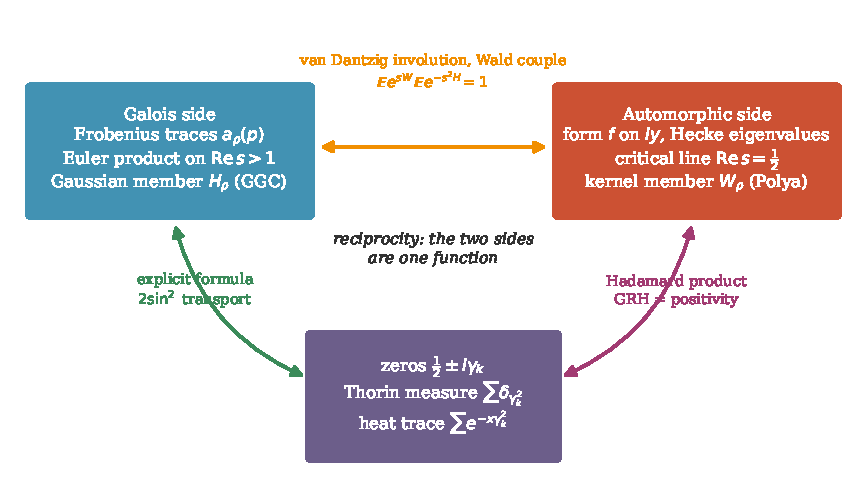
\includegraphics[width=\textwidth]{figs/recip_swap.pdf}
\caption{One function, two faces. The Euler product on $\operatorname{Re}s>1$ carries the Galois data, the Mellin transform on the critical line carries the automorphic form, and the zeros sit between them. The explicit formula with the $2\sin^2$ transport, the Hadamard product, and the van Dantzig involution with its Wald couple pass between the three.}\label{fig:recipswap}
\end{figure}

\section{The reciprocity problem}\label{sec:recipproblem}

Let $\rho$ be an Artin representation of $\Gal(\overline\Q/\Q)$ on an $n$ dimensional complex vector space $V$ or, more generally, a geometric $\ell$ adic representation on an $n$ dimensional $\overline\Q_\ell$ vector space $V$, pure of weight $w$, made complex through a fixed isomorphism $\overline\Q_\ell\cong\C$. Its gamma factor $\gamma(s,\rho)$ is determined by the Hodge numbers and the action of complex conjugation, and $N_\rho$ is its conductor. For $p$ unramified put $a_\rho(p^m)=\tr\rho(\Frob_p^m)$. In the unitary normalisation ($s$ shifted by $w/2$; at $p=\ell$ the local factor is that of the associated Weil Deligne representation) the Euler product
\[
L(s,\rho)=\prod_p\det\bigl(1-\rho(\Frob_p)p^{-s}\bigm|V^{I_p}\bigr)^{-1}
\]
converges absolutely for $\operatorname{Re}s>1$, and $\Lambda(s,\rho)=N_\rho^{s/2}\gamma(s,\rho)L(s,\rho)$ is its completion (the factor $N_\rho^{s/2}$ is kept out of $\gamma(s,\rho)$, unlike in Appendix~\ref{app:A}). Everything in $\Lambda(s,\rho)$ for $\operatorname{Re}s>1$ is Galois data: Frobenius traces, the conductor and the gamma factor. For Artin representations, Brauer's induction theorem \cite{brauer1947} gives meromorphic continuation and the functional equation $\Lambda(s,\rho)=\varepsilon(\rho)\Lambda(1-s,\check\rho)$; Artin's conjecture \cite{artin1924} asserts that $\Lambda(s,\rho)$ is entire when $\rho$ has no trivial constituent.

\begin{conjecture}[Langlands reciprocity \cite{langlands1970}]\label{conj:recip}\index{reciprocity conjecture}
For every irreducible $\rho$ as above there is a cuspidal automorphic representation $\pi$ of $\GL_n(\A_\Q)$ with $L(s,\rho_p)=L(s,\pi_p)$ for every place $p$.
\end{conjecture}

For $n=1$ this is class field theory (Artin's reciprocity law \cite{artin1927}). For $n=2$ it is known for Artin representations with solvable image, odd or even, by Hecke, Langlands and Tunnell \cite{langlands1980,tunnell1981}, for all odd ones as a consequence of Serre's conjecture, proved by Khare and Wintenberger \cite{kharewintenberger2009,kharewintenberger2009b} with work of Kisin \cite{kisin2009}, and for elliptic curves over $\Q$ by Wiles, Taylor and Wiles, and Breuil, Conrad, Diamond and Taylor \cite{wiles1995,taylorwiles1995,bcdt2001}. Potential automorphy \cite{hsbt2010,blght2011} gave meromorphic continuation and functional equations for the symmetric powers of holomorphic newforms, and Newton and Thorne \cite{newtonthorne2021,newtonthorne2021b} proved them automorphic for newforms of weight at least two without complex multiplication (Chapter~\ref{ch:03}). In dimension two the even icosahedral case is open.

The analytic route to reciprocity runs through converse theorems.\index{converse theorem} Hecke \cite{hecke1936} showed that a Dirichlet series whose completion is entire, bounded in vertical strips and satisfies the level one functional equation comes from a modular form for $\SL_2(\Z)$ (Section~\ref{sec:02mellin}). Weil \cite{weil1967} added twists by Dirichlet characters to reach $\Gamma_0(N)$; Jacquet and Langlands \cite{jacquetlanglands1970} recast this for $\GL_2$, and Cogdell and Piatetski Shapiro \cite{cogdellps1994} extended it to $\GL_n$, with twists by cuspidal representations $\pi'$ of $\GL_m$, $m\le n-1$. So, once the local Langlands correspondence has fixed the local components of the candidate $\pi$, reciprocity for $\rho$ follows from \emph{analytic} properties of the twisted $L$ functions $L(s,\rho\times\pi')$: continuation, holomorphy, boundedness and functional equations (Open Problem~\ref{op:inverse} asks for a probabilistic counterpart of these theorems). Booker \cite{booker2006} turned this into a computation, verifying Artin's conjecture up to a finite height for some nonmonomial representations with $A_5$ and $S_5$ image (Section~\ref{sec:recipswap}).

\section{Quadratic reciprocity from the Gaussian law}\label{sec:recipgauss}

For quadratic characters the analytic content of reciprocity is one probabilistic fact: the characteristic function of a normal law is a Gaussian. Here it is applied to a single random variable, the position at a fixed time of a Brownian motion wrapped around a circle. None of the theorems of this section is new, apart from the explicit bounds (i) and (ii) of Theorem~\ref{thm:recipheat}, which are elementary; the route shows which part of the classical reciprocity laws is probability.

\begin{lemma}[wrapped Gaussian]\label{lem:recipwrap}\index{Poisson summation}
For $x>0$ and real $y$,
\[
\sum_{k\in\Z}e^{-xk^2+iky}=\sqrt{\frac\pi x}\,\sum_{n\in\Z}e^{-(y+2\pi n)^2/(4x)} .
\]
\end{lemma}

\begin{proof}
Let $Y\sim N(0,2x)$, with density $\varphi(y)=(4\pi x)^{-1/2}e^{-y^2/(4x)}$, and let $\varphi_{2\pi}(y)=\sum_n\varphi(y+2\pi n)$ be the density of $Y$ reduced modulo $2\pi$. The series converges uniformly on compact sets, so $\varphi_{2\pi}$ is continuous and $2\pi$ periodic, and its Fourier coefficients are $\int_0^{2\pi}\varphi_{2\pi}(y)e^{-iky}dy=\E e^{-ikY}=e^{-xk^2}$. These are absolutely summable, so the Fourier series of $\varphi_{2\pi}$ converges uniformly, and by Fej\'er's theorem its sum is $\varphi_{2\pi}$: $\varphi_{2\pi}(y)=(2\pi)^{-1}\sum_ke^{-xk^2}e^{iky}$ for every $y$. Multiplying by $2\pi$ gives the lemma.
\end{proof}

Put $\theta(\tau)=\sum_{n\in\Z}e^{\pi in^2\tau}$ for $\operatorname{Im}\tau>0$.

\begin{theorem}[theta transformation]\label{thm:reciptheta}\index{theta function}
$\theta(-1/\tau)=\sqrt{\tau/i}\;\theta(\tau)$, with the principal branch of the square root.
\end{theorem}

\begin{proof}
Lemma~\ref{lem:recipwrap} with $y=0$ and $x=\pi t$ gives $\theta(it)=t^{-1/2}\theta(i/t)$ for $t>0$, which is the claim on the imaginary axis, since $-1/(it)=i/t$ and $\sqrt{it/i}=\sqrt t$. Both sides are holomorphic on the upper half plane, because $\tau/i$ has positive real part there, so they agree everywhere.
\end{proof}

We need one elementary estimate. If $h\in C^1(\R)$ with $h$ and $h'$ integrable, then for $t_0\in\R$ and $\eta>0$,
\begin{equation}\label{eq:recipriemann}
\Bigl|\eta\sum_{m\in\Z}h(t_0+m\eta)-\int_{\R}h\Bigr|\le\eta\int_{\R}|h'| ,
\end{equation}
because on each interval $[t_0+m\eta,t_0+(m+1)\eta]$ the difference between $\eta h(t_0+m\eta)$ and the integral of $h$ is at most $\eta$ times the integral of $|h'|$ over that interval.

For integers $a,c\ge1$ with $ac$ even put
\[
S(a,c)=\sum_{n\bmod c}e^{\pi ian^2/c}=c\,\E e^{\pi iaU^2/c},\qquad U\text{ uniform on }\Z/c\Z .
\]
The summand depends only on $n$ modulo $c$, because $a(n+c)^2/c=an^2/c+2an+ac$ and $ac$ is even.

\begin{theorem}[reciprocity for Gauss sums; Schaar, Landsberg]\label{thm:recipls}\index{Gauss sum}
For integers $a,c\ge1$ with $ac$ even,
\[
\frac1{\sqrt c}\,S(a,c)=\frac{e^{\pi i/4}}{\sqrt a}\;\overline{S(c,a)} .
\]
\end{theorem}

\begin{proof}
Let $\tau=a/c+i\varepsilon$ with $\varepsilon>0$; we let $\varepsilon\downarrow0$, so that $\theta(\tau)/\theta(i\varepsilon)$ is the characteristic function of the square of a discrete Gaussian of variance of order $\varepsilon^{-1}$, evaluated at $\pi a/c$. Grouping $n$ by its residue $r$ modulo $c$,
\[
\theta(\tau)=\sum_{r\bmod c}e^{\pi iar^2/c}\sum_{m\in\Z}e^{-\pi\varepsilon(r+mc)^2}.
\]
By \eqref{eq:recipriemann} with $h(u)=e^{-\pi u^2}$ and $\eta=c\sqrt\varepsilon$, $\sqrt\varepsilon\sum_me^{-\pi\varepsilon(r+mc)^2}\to1/c$, so $\sqrt\varepsilon\,\theta(\tau)\to S(a,c)/c$: the discrete Gaussian reduced modulo $c$ becomes uniform.

On the other side, $-1/\tau=-c/a+w$ with $w=i\delta/(1+i\kappa)$, $\delta=c^2\varepsilon/a^2$ and $\kappa=c\varepsilon/a$. Hence $e^{\pi in^2(-1/\tau)}=e^{-\pi icn^2/a}e^{-\pi\delta\beta n^2}$ with $\beta=(1+i\kappa)^{-1}$, and the first factor depends only on $n$ modulo $a$. Grouping by residues modulo $a$ and applying \eqref{eq:recipriemann} to $h_\beta(u)=e^{-\pi\beta u^2}$ with $\eta=a\sqrt\delta$, where $\int|h_\beta'|$ is bounded for $|\kappa|\le1$ and $\int h_\beta=\beta^{-1/2}\to1$, we get $\sqrt\delta\,\theta(-1/\tau)\to\overline{S(c,a)}/a$. Since $\sqrt\delta=(c/a)\sqrt\varepsilon$, this says $\sqrt\varepsilon\,\theta(-1/\tau)\to\overline{S(c,a)}/c$.

Now multiply the identity of Theorem~\ref{thm:reciptheta} by $\sqrt\varepsilon$ and let $\varepsilon\downarrow0$. Since $\sqrt{\tau/i}\to\sqrt{a/c}\,e^{-\pi i/4}$, we get $\overline{S(c,a)}/c=\sqrt{a/c}\,e^{-\pi i/4}S(a,c)/c$, which is the theorem.
\end{proof}

\begin{corollary}[Gauss's sign]\label{cor:recipgausssign}
For odd $m\ge1$, $g(m)=\sum_{n\bmod m}e^{2\pi in^2/m}$ equals $\sqrt m$ if $m\equiv1\bmod4$ and $i\sqrt m$ if $m\equiv3\bmod4$.
\end{corollary}

\begin{proof}
Take $a=2$, $c=m$: $g(m)=S(2,m)=\sqrt{m/2}\,e^{\pi i/4}(1+e^{-\pi im/2})$. For $m\equiv1\bmod4$, $1+e^{-\pi im/2}=1-i=\sqrt2e^{-\pi i/4}$; for $m\equiv3\bmod4$ it is $1+i=\sqrt2e^{\pi i/4}$.
\end{proof}

Gauss conjectured the sign in 1801, found a proof only in 1805 and published it in 1811 \cite{gauss1811}. Here it is the limit point of the curve $\varepsilon\mapsto\sqrt\varepsilon\,\theta(2/m+i\varepsilon)$ (Figure~\ref{fig:recipgauss}, left).

\begin{corollary}[quadratic reciprocity]\label{cor:recipqr}\index{quadratic reciprocity}
For distinct odd primes $p,q$,
\[
\Bigl(\frac pq\Bigr)\Bigl(\frac qp\Bigr)=(-1)^{\frac{p-1}2\frac{q-1}2},\qquad \Bigl(\frac{-1}p\Bigr)=(-1)^{\frac{p-1}2},\qquad\Bigl(\frac2p\Bigr)=(-1)^{\frac{p^2-1}8}.
\]
\end{corollary}

\begin{proof}
For $p\nmid k$ put $g_k(p)=\sum_{n\bmod p}e^{2\pi ikn^2/p}$. Since $n^2\equiv b$ has $1+(\frac bp)$ solutions, $g_k(p)=\sum_b(\frac bp)e^{2\pi ikb/p}=(\frac kp)g(p)$ after substituting $b\mapsto k^{-1}b$. By Proposition~\ref{prop:recipgood} below, $g(pq)=g_q(p)g_p(q)=(\frac qp)(\frac pq)g(p)g(q)$. Write $g(m)=\omega_m\sqrt m$ with $\omega_m\in\{1,i\}$ from Corollary~\ref{cor:recipgausssign}, which applies to the composite $m=pq$. Then $(\frac pq)(\frac qp)=\omega_{pq}/(\omega_p\omega_q)$, which is $1/i^2=-1$ when $p\equiv q\equiv3\bmod4$ and $1$ otherwise.

For the first supplement, $\overline{g(p)}=g_{-1}(p)=(\frac{-1}p)g(p)$, and $g(p)$ is real exactly when $p\equiv1\bmod4$. For the second, Theorem~\ref{thm:recipls} with $a=4$, $c=p$ gives $g_2(p)=S(4,p)=\frac{\sqrt p}2e^{\pi i/4}\sum_{n\bmod4}e^{-\pi ipn^2/4}=\frac{\sqrt p}2e^{\pi i/4}(1+2e^{-\pi ip/4}+e^{-\pi ip})=\sqrt p\,e^{\pi i(1-p)/4}$, so $(\frac2p)=e^{\pi i(1-p)/4}/\omega_p$, which is $1,-1,-1,1$ for $p\equiv1,3,5,7\bmod8$.
\end{proof}

The one step of the proof that does not use the Gaussian is finite Fourier analysis, and it has a statistical origin. For $m\ge1$ and $\gcd(k,m)=1$ let $\mathsf F_m^{(k)}=(e^{2\pi ikjl/m})_{j,l\bmod m}$, so that $\mathsf F_m=\mathsf F_m^{(1)}$ is the discrete Fourier transform matrix. Then $\tr\mathsf F_m^{(k)}=\sum_{j\bmod m}e^{2\pi ikj^2/m}$ is a Gauss sum, written $g_k(m)$, with $g_1(m)=g(m)$.

\begin{proposition}[Good's factorisation]\label{prop:recipgood}
Let $m=pq$ with $\gcd(p,q)=1$. Index rows and columns of $\mathsf F_m$ by $(x,y)\in\Z/p\Z\times\Z/q\Z$ through $j=xq+yp$. Then $\mathsf F_m$ becomes the tensor product $\mathsf F_p^{(q)}\otimes\mathsf F_q^{(p)}$, and taking traces, $g(pq)=g_q(p)\,g_p(q)$.
\end{proposition}

\begin{proof}
The map is a bijection by the Chinese remainder theorem, and for $j=xq+yp$, $l=x'q+y'p$ we have $jl/(pq)\equiv xx'q/p+yy'p/q\bmod1$. The trace is invariant under the simultaneous permutation of rows and columns and is multiplicative on tensor products.
\end{proof}

This index map is one of the two maps of Good's prime factor algorithm for the fast Fourier transform \cite{good1958}, which grew out of Yates's interaction algorithm for factorial experiments. In \cite{good1962} he set the discrete Fourier transform beside Fourier series and Fourier integrals, as the third member of a family of analogues, and proved a discrete Poisson summation formula: for $f$ on $\Z/N\Z$ with $N=mn$ and $f^*(r)=\sum_jf(j)e^{-2\pi ijr/N}$,
\[
\sum_{k\bmod n}f(km)=\frac1m\sum_{l\bmod m}f^*(ln).
\]
The proof of Corollary~\ref{cor:recipqr} uses all three of Good's analogues in turn: the Fourier integral is the normal characteristic function, the Fourier series the wrapped normal law of Lemma~\ref{lem:recipwrap}, and the discrete transform the Gauss sum and its factorisation. The Brownian limit of Theorem~\ref{thm:recipls} is the passage from the second to the third, turning the theta transformation into a statement about $\mathsf F_c$. Schur \cite{schur1921} gave a proof of Gauss's sign that stays entirely within the third analogue, by computing the multiplicities of the eigenvalues $\pm1,\pm i$ of $\mathsf F_m/\sqrt m$, whose trace is $g(m)/\sqrt m$. The Gaussian is the basic eigenfunction of the Fourier transform, with eigenvalue $1$, and the Brownian limit is in this sense the continuous shadow of Schur's argument.

In the language of Section~\ref{sec:recipproblem} the corollary is reciprocity for quadratic Galois characters: for $q\equiv1\bmod4$ the Frobenius character $p\mapsto(\frac qp)$ of $\Q(\sqrt q)$, a Galois object, equals the Dirichlet character $p\mapsto(\frac pq)$, an automorphic object for $\GL_1$. This is the simplest case of Conjecture~\ref{conj:recip}, a theorem since Gauss; what the Gaussian supplies is its analytic part.

\begin{figure}[t]
\centering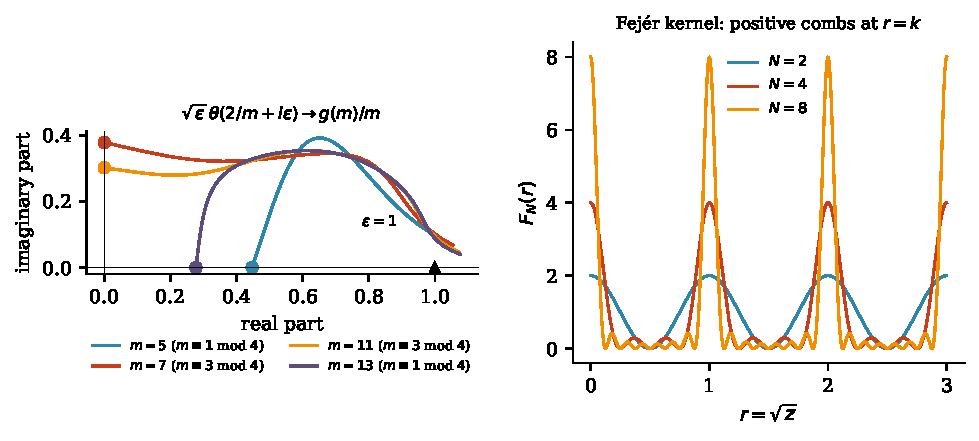
\includegraphics[width=\textwidth]{figs/recip_gauss.pdf}
\caption{Left: Theorem~\ref{thm:recipls} as a Brownian limit. The curves $\varepsilon\mapsto\sqrt\varepsilon\,\theta(2/m+i\varepsilon)$ for $m=5,7,11,13$, $10^{-5}\le\varepsilon\le1$, start near $1$ (triangle) and end at $g(m)/m$, which is real for $m\equiv1\bmod4$ and imaginary for $m\equiv3\bmod4$ (Corollary~\ref{cor:recipgausssign}). Right: the Fej\'er kernel $F_N(r)=\sin^2(\pi Nr)/(N\sin^2\pi r)$ for $N=2,4,8$, the positive combination of winding number cosines in Proposition~\ref{prop:recipfejer}; as $N$ grows it concentrates at the integers $r=k$, that is at the eigenvalues $z=k^2$.}\label{fig:recipgauss}
\end{figure}

The same lemma gives the functional equation of the $L$ function of every even primitive Dirichlet character (stated in Chapter~\ref{ch:02}), with its root number.

\begin{theorem}[the Dirichlet functional equation as a kernel symmetry]\label{thm:recipdirichlet}
Let $\chi$ be a primitive even character modulo $q>1$, $g(\chi)=\sum_{m\bmod q}\chi(m)e^{2\pi im/q}$ its Gauss sum, and $\theta_\chi(t)=\sum_{n\in\Z}\chi(n)e^{-\pi n^2t/q}$ for $t>0$. Then $\theta_\chi(1/t)=\frac{g(\chi)}{\sqrt q}\sqrt t\,\theta_{\bar\chi}(t)$. Equivalently, the P\'olya kernel $\Phi_\chi(u)=\theta_\chi(e^{2u})e^{u/2}$, which satisfies $\Lambda(\frac12+z,\chi)=\int\Phi_\chi(u)e^{zu}du$ for every complex $z$, where $\Lambda(s,\chi)=(q/\pi)^{s/2}\Gamma(s/2)L(s,\chi)$, obeys $\Phi_\chi(-u)=\frac{g(\chi)}{\sqrt q}\Phi_{\bar\chi}(u)$; that is, $\Lambda(s,\chi)=\frac{g(\chi)}{\sqrt q}\Lambda(1-s,\bar\chi)$.
\end{theorem}

\begin{proof}
Primitivity gives $\chi(n)=g(\bar\chi)^{-1}\sum_{m\bmod q}\bar\chi(m)e^{2\pi imn/q}$ for all $n$. Insert this into $\theta_\chi(t)$ and apply Lemma~\ref{lem:recipwrap} with $x=\pi t/q$ and $y=2\pi m/q$. The exponent becomes $(y+2\pi k)^2/(4x)=\pi(m+kq)^2/(qt)$, and $\ell=m+kq$ runs over the class of $m$, so $\theta_\chi(t)=g(\bar\chi)^{-1}\sqrt{q/t}\,\theta_{\bar\chi}(1/t)$. Since $g(\chi)g(\bar\chi)=\chi(-1)q=q$, this is the claim with $t$ and $1/t$ exchanged. The Mellin formula $\int_0^\infty e^{-\pi n^2t/q}t^{s/2}dt/t=\Gamma(s/2)(q/\pi n^2)^{s/2}$ gives $\Lambda(s,\chi)=\frac12\int_0^\infty\theta_\chi(t)t^{s/2}dt/t$, and $t=e^{2u}$ gives the kernel form.
\end{proof}

For a real even primitive $\chi$ the root number $g(\chi)/\sqrt q$ is $\pm1$, since $g(\chi)^2=q$. Whether the P\'olya kernel is even or odd is therefore a sign problem, and for $\chi=(\frac\cdot q)$ with $q\equiv1\bmod4$ prime, $g(\chi)=g(q)=\sqrt q$ by Corollary~\ref{cor:recipgausssign}. So \emph{for primes $q\equiv1\bmod4$, Gauss's sign theorem is the statement that a P\'olya kernel is even}, the $\GL_1$ analogue of Proposition~\ref{prop:recipsym}, and the Brownian limit of Figure~\ref{fig:recipgauss} decides it.

\subsection{The swap for the circle}

The theta transformation can also be proved by a positivity argument, with the Laplace pair of the $2\sin^2$ lemma (compare Section~\ref{sec:recipswap}). Write $\cos u\sqrt z=1-2\sin^2(u\sqrt z/2)$ in \eqref{eq:10dpair} with $a=u^2/4$; since $\int_0^\infty e^{-xz}(\pi z)^{-1/2}dz=x^{-1/2}$ this gives
\begin{equation}\label{eq:recipcospair}
\sqrt{\frac\pi x}\,e^{-u^2/(4x)}=\int_0^\infty e^{-xz}\cos(u\sqrt z)\,\frac{dz}{\sqrt z} .
\end{equation}
The circle $\R/2\pi\Z$ has Laplace eigenvalues $k^2$, $k\in\Z$, playing the part of the $\gamma^2$, and closed geodesics of lengths $2\pi|n|$, playing the part of the prime powers. Its heat trace is $\sum_ke^{-xk^2}$, the Laplace transform of the comb $\sum_{k\in\Z}\delta_{k^2}$, which is the local Thorin comb $\tau_{0,2\pi}$ of Theorem~\ref{thm:10clocal} in its degenerate case $\theta=0$ (Exercise~\ref{ex:10cdegenerate}); \eqref{eq:recipcospair} with $u=2\pi n$ attaches to each winding number $n$ the cosine density $\cos(2\pi n\sqrt z)z^{-1/2}$, a Fourier mode of this comb. In the same way the explicit formula attaches to each prime power $p^m$ a multiple of the cosine density $\cos(m\sqrt z\log p)z^{-1/2}$ (Proposition~\ref{prop:reciprigid}), which by Proposition~\ref{prop:10cdictionary} is, up to sign and the factor $p^{-m/2}$, the $m$th Fourier mode of the local Thorin comb of $p$.

\begin{proposition}[Fej\'er positivity for the circle]\label{prop:recipfejer}\index{Fej\'er kernel}
For $N\ge1$ and $x>0$ let $\mathcal W_N(x)=\sqrt{\pi/x}\sum_{|n|<N}(1-|n|/N)e^{-\pi^2n^2/x}$. Then
\[
\mathcal W_N(x)=\int_0^\infty e^{-xz}F_N(\sqrt z)\frac{dz}{\sqrt z},\qquad F_N(r)=\sum_{|n|<N}\Bigl(1-\frac{|n|}N\Bigr)\cos2\pi nr ,
\]
where $F_N(r)=\sin^2(\pi Nr)/(N\sin^2\pi r)\ge0$ is Fej\'er's kernel, so every $\mathcal W_N$ is completely monotone. As $N\to\infty$ the measures $F_N(\sqrt z)z^{-1/2}dz$ converge vaguely to the comb $\sum_{k\in\Z}\delta_{k^2}=\delta_0+2\sum_{k\ge1}\delta_{k^2}$, and consequently $\sqrt{\pi/x}\sum_ne^{-\pi^2n^2/x}=\sum_ke^{-xk^2}$.
\end{proposition}

\begin{proof}
The integral formula is \eqref{eq:recipcospair} summed with the Fej\'er weights, and the closed form of $F_N$ is classical. In the variable $r=\sqrt z$ the measure is $2F_N(r)dr$ on $[0,\infty)$. The Fej\'er kernel is $1$ periodic, nonnegative, of mass $1$ over a period, and tends to zero uniformly away from the integers; so $2F_N(r)dr$ converges vaguely to $2\sum_{k\ge1}\delta_k+\delta_0$, the half mass at $0$ coming from the half bump on $[0,\frac12]$. The tails are uniformly small, since $\int_{r>R}e^{-xr^2}2F_N(r)dr\le2\sum_{k\ge\lfloor R\rfloor}e^{-xk^2}$, so the Laplace transforms converge: $\mathcal W_N(x)\to1+2\sum_{k\ge1}e^{-xk^2}$. The left side converges to $\sqrt{\pi/x}\sum_ne^{-\pi^2n^2/x}$ by dominated convergence.
\end{proof}

In the variable $r=\sqrt z$, \eqref{eq:recipcospair} is again the normal characteristic function, and the proof is Fej\'er's proof of Poisson summation written as a Laplace transform; it proves Theorem~\ref{thm:reciptheta}, hence Corollaries~\ref{cor:recipgausssign} and \ref{cor:recipqr}, a second time. Its shape is that of Theorem~\ref{thm:recipcm}: the geodesic side, summed with positive weights, is the Laplace transform of a positive measure, which turns out to be the spectral measure. For the circle positivity is free, because the Fej\'er kernel is a square. For an $L$ function the prime powers enter with the signed weights $-\Lambda_\rho(n)n^{-1/2}$ of Definition~\ref{def:recipheat}, and the archimedean term is not positive either: its density $\log N_\rho+2\operatorname{Re}\frac{\gamma'}{\gamma}(\frac12+it,\rho)$ is smallest at $t=0$, where it is negative for $\zeta$, $\Delta$ and the Artin representation of conductor $23$. A Fej\'er type positive summation of the right side of Definition~\ref{def:recipheat} would prove, through Theorem~\ref{thm:recipcm}, holomorphy and GRH at once (Open Problem~\ref{op:recipfejer}).

\subsection{Heat flow and generalized Gauss sums}

For integers $a,c\ge1$ with $ac$ even and $k\in\Z$ put
\[
S(a,c;k)=\sum_{r\bmod c}e^{\pi i(ar^2+2kr)/c},
\]
so that $S(a,c;0)$ is the Gauss sum of Theorem~\ref{thm:recipls}. For $\varepsilon>0$ let $X_\varepsilon$ be the discrete Gaussian, $\Prob(X_\varepsilon=n)=e^{-\pi\varepsilon n^2}/\theta(i\varepsilon)$.

\begin{theorem}[heat flow reciprocity]\label{thm:recipheat}
Let $u=e^{-\pi/(c^2\varepsilon)}$.
\begin{enumerate}
\item[(i)] For every $r$,
\[
\Prob(X_\varepsilon\equiv r\bmod c)=\frac{\sum_ke^{-\pi k^2/(c^2\varepsilon)}e^{2\pi ikr/c}}{c\sum_ke^{-\pi k^2/\varepsilon}},
\]
and the total variation distance from the uniform law on $\Z/c\Z$ is at most $2u/(1-u)$.
\item[(ii)] $\bigl|\E e^{\pi iaX_\varepsilon^2/c}-S(a,c;0)/c\bigr|\le4u/(1-u)$.
\item[(iii)] With $\tau=a/c+i\varepsilon$ and $\kappa=c\varepsilon/a$, for every $\varepsilon>0$,
\[
\begin{split}
&\sqrt{\tau/i}\,\sum_{k\in\Z}e^{-\pi k^2/(c^2\varepsilon)}S(a,c;k)\\
&\qquad=\sqrt{1+i\kappa}\,\sum_{k\in\Z}e^{-\pi k^2(1+i\kappa)/(c^2\varepsilon)}\,\overline{S(c,a;k)} .
\end{split}
\]
\item[(iv)] Consequently, for every $k$,
\[
S(a,c;k)=\sqrt{c/a}\;e^{\pi i/4}\,e^{-\pi ik^2/(ac)}\,\overline{S(c,a;k)}.
\]
\end{enumerate}
\end{theorem}

\begin{proof}
(i) Group $n$ by residue and apply Lemma~\ref{lem:recipwrap} (Poisson summation) to
\[
\sum_me^{-\pi\varepsilon(r+mc)^2}=(c\sqrt\varepsilon)^{-1}\sum_ke^{-\pi k^2/(c^2\varepsilon)}e^{2\pi ikr/c},
\]
and to the normaliser $\theta(i\varepsilon)=\varepsilon^{-1/2}\sum_ke^{-\pi k^2/\varepsilon}$. The difference from $1/c$ is at most
\[
c^{-1}\Bigl(2\sum_{k\ge1}u^{k^2}+2\sum_{k\ge1}e^{-\pi k^2/\varepsilon}\Bigr)\le4c^{-1}\sum_{k\ge1}u^{k^2}
\]
since the denominator is at least $1$, and summing over $r$ and halving gives the bound. (ii) $|e^{\pi iar^2/c}|=1$ and $e^{\pi iar^2/c}$ depends only on $r\bmod c$, so the difference is at most twice the total variation distance. (iii) As in (i), $\sqrt\varepsilon\,\theta(\tau)=c^{-1}\sum_ke^{-\pi k^2/(c^2\varepsilon)}S(a,c;k)$. On the other side $-1/\tau=-c/a+i\delta/(1+i\kappa)$ with $\delta=c^2\varepsilon/a^2$, and Poisson summation with the complex Gaussian weights $e^{-\pi\delta(r+ma)^2/(1+i\kappa)}$ (Lemma~\ref{lem:recipwrap} continued analytically to $\operatorname{Re}x>0$, both sides being holomorphic in $x$) gives
\[
\theta(-1/\tau)=\frac{\sqrt{1+i\kappa}}{c\sqrt\varepsilon}\sum_ke^{-\pi k^2(1+i\kappa)/(c^2\varepsilon)}\overline{S(c,a;-k)}.
\] The theta transformation $\theta(-1/\tau)=\sqrt{\tau/i}\,\theta(\tau)$ and $S(c,a;-k)=S(c,a;k)$ give (iii). (iv) Since $\tau=(a/c)(1+i\kappa)$ and $\kappa/(c^2\varepsilon)=1/(ac)$, (iii) reads
\[
\sum_kw_k\Bigl[\sqrt{a/c}\,e^{-\pi i/4}S(a,c;k)-e^{-\pi ik^2/(ac)}\overline{S(c,a;k)}\Bigr]=0
\]
with $w_k=e^{-\pi k^2/(c^2\varepsilon)}$, for every $\varepsilon>0$. The terms for $k$ and $-k$ coincide, and the functions $\varepsilon\mapsto e^{-\pi k^2/(c^2\varepsilon)}$, $k\ge0$, are Laplace transforms in $1/\varepsilon$ of distinct point masses, so letting $1/\varepsilon\to\infty$ and peeling off the terms one exponent $k^2$ at a time, using that the brackets are bounded, shows that every bracket vanishes.
\end{proof}

Part (iv) is the reciprocity law for generalized quadratic Gauss sums with even linear term (Berndt, Evans and Williams \cite{bew1998}, Theorem~1.2.2). The proof shows that the whole family is a single identity, (iii), between two Gaussian mixtures, which the theta transformation and uniqueness of Laplace transforms separate into its components. At $\varepsilon\downarrow0$ only $k=0$ survives and (iii) becomes the reciprocity of Schaar and Landsberg. Part (i) quantifies the Brownian limit of Theorem~\ref{thm:recipls}: the residue of a discrete Gaussian is uniform up to $e^{-\pi/(c^2\varepsilon)}$ (Figure~\ref{fig:recipzero}, right: for the plotted $c=5$, $7$ and $12$, wherever the bound is below $0.1$ it exceeds the distance by a factor between $3$ and $3.4$). Numerically, (iii) holds to $3\cdot10^{-40}$ at forty digit precision for the four parameter sets tested, and (iv) to $10^{-47}$ at fifty digit precision for all $a,c\le24$ with $ac$ even and $|k|\le6$.

\section{Reciprocity as an identity between random variables}\label{sec:reciplaw}

This section restates reciprocity and its first consequences in the language of probability. The analytic inputs are classical (Brauer's induction theorem, Hecke $L$ functions, the Rankin Selberg method); granted them, the proofs are short and show which part of each statement is probability and which is arithmetic.

\subsection{The Frobenius probability space}

Fix a finite set $S$ of primes and $\sigma>1$. Let $\Omega_S$ be the set of prime powers $p^m$ with $p\notin S$, $m\ge1$, and let $\Prob_\sigma$, Dirichlet's measure, be the probability measure
\[
\Prob_\sigma(\{p^m\})=\frac{p^{-m\sigma}}{m\,Z_\sigma},\qquad Z_\sigma=\sum_{p\notin S,\,m\ge1}\frac{p^{-m\sigma}}m=\log\zeta^S(\sigma)=\log\frac1{\sigma-1}+O(1),
\]
where $\zeta^S$, like $L^S$ below, omits the Euler factors at $S$, and $O(1)$ refers to $\sigma\downarrow1$. A Galois representation $\rho$ as in Section~\ref{sec:recipproblem}, unramified outside $S$ and in the unitary normalisation, so that its Frobenius eigenvalues have absolute value $1$, defines the random variable $a_\rho(p^m)=\tr\rho(\Frob_p^m)$, and when $\rho$ factors through a finite group $G=\Gal(K/\Q)$ it defines the random conjugacy class $F(p^m)=\Frob_p^m$ of $G$. A unitary cuspidal automorphic representation $\pi$ of $\GL_n(\A_\Q)$ unramified outside $S$, with Satake parameters $\{\alpha_{1,p},\dots,\alpha_{n,p}\}$, defines $a_\pi(p^m)=\sum_i\alpha_{i,p}^m$. The definitions are made so that
\begin{equation}\label{eq:reciplogL}
\E_\sigma\bigl[a\,\bar b\,\bigr]=\frac1{Z_\sigma}\log L^S(\sigma,\,\cdot\,)
\end{equation}
for the Rankin Selberg $L$ function of the pair: $L^S(\sigma,\rho\otimes\check\rho')$ for two Galois representations, $L^S(\sigma,\pi\times\tilde\pi')$ for two automorphic ones, the logarithm being the one given by the Dirichlet series. This uses $\overline{\tr\rho'(\Frob_p^m)}=\tr\check\rho'(\Frob_p^m)$ and, for unitary $\pi'$, that the Satake parameters of $\tilde\pi'$ are the conjugates of those of $\pi'$. For $\pi\times\tilde\pi$ the coefficients $|a_\pi(p^m)|^2$ are nonnegative and the series converges for $\sigma>1$ by Jacquet and Shalika \cite{jacquetshalika1981} (Theorem~\ref{thm:ch09rs}); Cauchy Schwarz then gives absolute convergence for every pair. In particular all these variables are square integrable under $\Prob_\sigma$.

\begin{proposition}[reciprocity is almost sure equality]\label{prop:recipas}
Let $\rho$ be an $n$ dimensional Galois representation and $\pi$ a cuspidal automorphic representation of $\GL_n(\A_\Q)$, both unramified outside $S$. Then $L(s,\rho_p)=L(s,\pi_p)$ for all $p\notin S$ if and only if $a_\rho=a_\pi$ $\Prob_\sigma$ almost surely, for one and then every $\sigma>1$.
\end{proposition}

\begin{proof}
$\Prob_\sigma$ charges every point of $\Omega_S$, so almost sure equality is equality at every $p^m$. The power sums $a(p^m)$, $m\ge1$, of $n$ numbers determine their elementary symmetric functions by Newton's identities, hence the characteristic polynomial of $\rho(\Frob_p)$ and the multiset of Satake parameters, hence the local factor; the converse is immediate.
\end{proof}

So Conjecture~\ref{conj:recip}, weakened to agreement at the primes outside a set $S$ containing those where $\rho$ ramifies, is an existence statement about random variables on $(\Omega_S,\Prob_\sigma)$: every Frobenius trace variable $a_\rho$ of an irreducible $\rho$ is almost surely equal to a Hecke eigenvalue variable $a_\pi$ of a cuspidal $\pi$.

\subsection{Chebotarev as convergence in law}

Everything on the Galois side rests on one lemma about Artin $L$ functions of virtual characters, a consequence of Brauer's induction theorem (Section~\ref{sec:ch3artin}).

\begin{lemma}\label{lem:recipvirtual}
Let $K/\Q$ be finite Galois with group $G$, unramified outside $S$, let $\psi$ be a virtual character of $G$, and let $e=\langle\psi,\mathsf{1}\rangle_G$. Then $(s-1)^eL(s,\psi)$ is holomorphic and nonzero near $s=1$, and $\log L^S(\sigma,\psi)=e\log\frac1{\sigma-1}+O(1)$ as $\sigma\downarrow1$.
\end{lemma}

\begin{proof}
By Brauer $\psi=\sum_in_i\operatorname{Ind}_{H_i}^G\chi_i$ with one dimensional $\chi_i$, so $L(s,\psi)=\prod_iL(s,\chi_i)^{n_i}$ with Hecke $L$ functions, each holomorphic and nonzero at $s=1$ except for a simple pole when $\chi_i$ is trivial. The order of the pole is $\sum_in_i\langle\chi_i,\mathsf{1}\rangle_{H_i}$, which is $\langle\psi,\mathsf{1}\rangle_G$ by Frobenius reciprocity. Removing finitely many Euler factors changes nothing near $1$, and the logarithm defined by the Dirichlet series is a continuous branch on $(1,2]$, so it differs from $e\log\frac1{\sigma-1}$ by the logarithm of a continuous nonvanishing function with a limit at $1$.
\end{proof}

\begin{theorem}[Chebotarev in law \cite{chebotarev1926} and the Frobenius distance]\label{thm:recipcheb}\index{Chebotarev density theorem}\index{Frobenius distance}
Let $K/\Q$ be finite Galois with group $G$, unramified outside $S$. Under $\Prob_\sigma$ the random class $F$ converges in law, as $\sigma\downarrow1$, to the image of Haar measure $\mu_G$ on conjugacy classes. Consequently, for Artin representations $\rho,\rho'$ factoring through $G$,
\begin{gather*}
\E_\sigma\bigl[a_\rho\overline{a_{\rho'}}\bigr]\to\langle\chi_\rho,\chi_{\rho'}\rangle_G,\\
d(\rho,\rho')^2:=\lim_{\sigma\downarrow1}\E_\sigma|a_\rho - a_{\rho'}|^2=\int_G|\chi_\rho - \chi_{\rho'}|^2\,d\mu_G .
\end{gather*}
In particular $d(\rho,\rho')=0$ if and only if $\rho\cong\rho'$, and $d(\rho,\rho')^2=2$ for nonisomorphic irreducible $\rho,\rho'$.
\end{theorem}

\begin{proof}
By \eqref{eq:reciplogL} and Lemma~\ref{lem:recipvirtual}, $\E_\sigma\chi(F)=\log L^S(\sigma,\chi)/Z_\sigma\to\langle\chi,\mathsf{1}\rangle_G=\int\chi\,d\mu_G$ for every irreducible character $\chi$. Irreducible characters span the class functions, so $\Prob_\sigma(F\in C)\to|C|/|G|$ for every class $C$, which is convergence in law on the finite set of classes. The remaining statements apply this to the class functions $\chi_\rho\overline{\chi_{\rho'}}$ and $|\chi_\rho-\chi_{\rho'}|^2$, and use that a representation is determined by its character and that irreducible characters are orthonormal.
\end{proof}

The theorem is the Dirichlet density form of Chebotarev's theorem \cite{chebotarev1926}, with the standard proof through Artin $L$ functions rather than Chebotarev's own (Section~\ref{sec:ch3cheb}); the natural density form is Corollary~\ref{cor:ch3cheb}. Only the language is new, and it is worth having for three reasons. First, $d$ is a pseudometric, and by the theorem a metric on isomorphism classes of Artin representations: $\|f\|_\sigma=(\E_\sigma|f|^2)^{1/2}$ is a seminorm, so Minkowski's inequality gives the triangle inequality for $d$ (with $\limsup$ in place of $\lim$ when the limit is not known to exist). Second, the theorem is a statement about couplings: for Artin representations $\rho:G\to\GL_n$, $\rho':G'\to\GL_{n'}$ the pair $(F,F')$ of Frobenius classes lives on one space, and Theorem~\ref{thm:recipcheb} applied to the compositum says that it converges in law to the image of Haar measure of the fibre product $H=\Gal(KK'/\Q)$, embedded in $G\times G'$ by restriction. Third, the theorem separates two levels of information that are easily confused: the \emph{marginal} law of $a_\rho$ (the Sato Tate law of $\rho$, the image of $\mu_G$ under $\chi_\rho$), and the \emph{joint} law of $(a_\rho,a_{\rho'})$.

Marginal laws cannot detect reciprocity (Proposition~\ref{prop:01limits}), but joint laws see more: the limiting joint law of $(a_\rho,a_{\rho'})$ separates nonisomorphic Artin representations with the same marginal law, and at each fixed $\sigma$ reciprocity says that the joint law of $(a_\rho,a_\pi)$ is carried by the diagonal (Proposition~\ref{prop:recipas}). Take $\rho$ the $S_3$ representation of $x^3-x-1$ and $\rho_{31}$ the $S_3$ representation of $x^3+x+1$, of conductor $31$. Their limiting marginal laws are identical (compare Example~\ref{ex:ch3cubic}): $a=2,0,-1$ with probabilities $\frac16,\frac12,\frac13$. The splitting fields are linearly disjoint, since their quadratic subfields $\Q(\sqrt{-23})$ and $\Q(\sqrt{-31})$ differ, so $H=S_3\times S_3$, the coupling is the independent one, and $d(\rho,\rho_{31})^2=2$. Over the $78496$ primes below $10^6$ other than $23$ and $31$ the empirical joint law of $(a_\rho(p),a_{\rho_{31}}(p))$ agrees with the product law $\frac1{36},\frac1{12},\dots,\frac19$ to within $0.0007$ in every cell.

\subsection{Cuspidal orthonormality on the automorphic side}

The automorphic analogue of Theorem~\ref{thm:recipcheb} is the Rankin Selberg method.

\begin{theorem}[orthonormality of cuspidal representations \cite{jpss1983,jacquetshalika1981,moeglinwaldspurger1989,shahidi1981}]\label{thm:recipcusp}
Let $\pi,\pi'$ be unitary cuspidal automorphic representations of $\GL_n(\A_\Q)$ and $\GL_{n'}(\A_\Q)$, unramified outside $S$. Then $\E_\sigma[a_\pi\overline{a_{\pi'}}]\to\delta_{\pi\cong\pi'}$ as $\sigma\downarrow1$. Hence $d(\pi,\pi')^2=2$ when $\pi\not\cong\pi'$, and $d(\pi,\pi')=0$ forces $\pi\cong\pi'$.
\end{theorem}

\begin{proof}
By Jacquet, Piatetski Shapiro and Shalika for $n\ne n'$, and by Jacquet and Shalika and Moeglin and Waldspurger for $n=n'$, $L(s,\pi\times\tilde\pi')$ is holomorphic at $s=1$ unless $\pi'\cong\pi$, when it has a simple pole, and by Shahidi it does not vanish on $\operatorname{Re}s=1$. The argument of Lemma~\ref{lem:recipvirtual} gives $\log L^S(\sigma,\pi\times\tilde\pi')=\delta_{\pi\cong\pi'}\log\frac1{\sigma-1}+O(1)$, and \eqref{eq:reciplogL} finishes the proof. For the distance expand $|a_\pi-a_{\pi'}|^2$.
\end{proof}

Theorems~\ref{thm:recipcheb} and \ref{thm:recipcusp} are one statement on two sides:\index{Schur orthogonality} irreducible Artin representations and cuspidal automorphic representations are both orthonormal systems of random variables in the limit $\sigma\downarrow1$, with unit second moment (the exponential law of Theorem~\ref{thm:recipgamma} below). For irreducible $\ell$ adic representations orthonormality is a conjecture of Tate type \cite{tate1965}, on the pole of $L(s,\rho\otimes\check\rho')$ at $s=1$. Strong multiplicity one\index{strong multiplicity one} follows in one line, by the argument of Jacquet and Shalika \cite{jacquetshalika1981}: if the local factors of two cuspidal representations agree outside a finite set of primes, enlarge $S$ to contain it; then $a_\pi=a_{\pi'}$ on $\Omega_S$, so $d(\pi,\pi')=0$ and $\pi\cong\pi'$.

\subsection{Reciprocity in law}

Call $\rho$ and $\pi$ \emph{reciprocal in law}\index{reciprocity in law} if $d(\rho,\pi)=0$, that is $\E_\sigma|a_\rho-a_\pi|^2\to0$ as $\sigma\downarrow1$.

\begin{corollary}[this book]\label{cor:reciplaw}
Let $\rho,\rho'$ be Artin representations and $\pi,\pi'$ unitary cuspidal automorphic representations, all unramified outside $S$.
\begin{enumerate}
\item[(i)] If $\rho$ and $\pi$ correspond in the sense of Conjecture~\ref{conj:recip}, they are reciprocal in law.
\item[(ii)] If $\rho$ is reciprocal in law with $\pi$ and with $\pi'$, then $\pi\cong\pi'$. If $\rho$ and $\rho'$ are both reciprocal in law with $\pi$, then $\rho\cong\rho'$.
\item[(iii)] If $\rho$ is reciprocal in law with a cuspidal $\pi$, then $\rho$ is irreducible.
\item[(iv)] If $\rho$ is reciprocal in law with $\pi$, then for every $\epsilon>0$ the primes with $|a_\rho(p)-a_\pi(p)|>\epsilon$ have Dirichlet density zero.
\item[(v)] If $\rho$ is automorphic, corresponding to $\pi_0$ in the sense of Conjecture~\ref{conj:recip}, then $\rho$ is reciprocal in law with $\pi$ only for $\pi\cong\pi_0$.
\end{enumerate}
\end{corollary}

\begin{proof}
(i) is Proposition~\ref{prop:recipas} after enlarging $S$. For (ii), the triangle inequality gives $d(\pi,\pi')\le d(\pi,\rho)+d(\rho,\pi')=0$, and Theorem~\ref{thm:recipcusp} applies; likewise $d(\rho,\rho')=0$ and Theorem~\ref{thm:recipcheb} applies. For (iii), Minkowski gives $|\|a_\rho\|_\sigma-\|a_\pi\|_\sigma|\le\|a_\rho-a_\pi\|_\sigma\to0$, while $\|a_\rho\|_\sigma^2\to\langle\rho,\rho\rangle$ and $\|a_\pi\|_\sigma^2\to1$; so $\langle\rho,\rho\rangle=1$. For (iv), with $E$ the set of such primes, $\sum_{p\in E}p^{-\sigma}/Z_\sigma\le\Prob_\sigma(|a_\rho-a_\pi|>\epsilon)\le\epsilon^{-2}\E_\sigma|a_\rho-a_\pi|^2\to0$ by Chebyshev's inequality. (v) is (i) and (ii).
\end{proof}

The corollary is the probabilistic skeleton of the reciprocity dictionary, each item a Hilbert space inequality from the two orthonormality theorems. The agreement in (iv) is only approximate: exact agreement, even on a set of density one, is open in general, and Open Problem~\ref{op:reciplaw} asks for it at all but finitely many primes. Nor does the corollary give existence, and it cannot: the powers of a set of primes of Dirichlet density zero carry $\Prob_\sigma$ mass $o(1)$, so reciprocity in law, like the laws of Proposition~\ref{prop:01limits}, is blind to bounded changes on such a set, while reciprocity itself is not. Figure~\ref{fig:reciplaw} shows the natural density version $\pi(X)^{-1}\sum_{p\le X}|a(p)-b(p)|^2$ of $d^2$ for six pairs. For $\rho$ and the weight one form $\eta(z)\eta(23z)$, whose coefficients were computed independently from the product expansion, it is exactly $0$ for all $X\le10^6$, a pointwise check of the reciprocity for $\rho$ proved by Hecke (Example~\ref{ex:ch3cubic}). For $\rho$ and the data $a'$ obtained from $a_\rho$ by moving $\Frob_2$ from a three cycle to the identity, as in Section~\ref{sec:recipfaces}, it is $1.1\cdot10^{-4}$ and tends to $0$: in law $a'$ is reciprocal to $\eta(z)\eta(23z)$. Yet no cuspidal representation has the local factors of $a'$ at every prime: it would be at distance $0$ from $\eta(z)\eta(23z)$, hence isomorphic to it by Theorem~\ref{thm:recipcusp}, and the Euler factors at $2$ differ. The P\'olya kernel and the Galois heat trace of the later sections do see this one change (Figures~\ref{fig:recipkernel} and \ref{fig:recipheat}). For the other four pairs, $(\rho,\chi_{-23})$, $(\rho,\rho_{31})$, $(\rho,\Delta)$ and $(\Delta,11a1)$, it is $2.000$, $1.998$, $2.005$ and $2.002$ at $X=10^6$, the value $2$ of two orthonormal vectors; over the same primes the mean squares of $a_\rho$ and of $\tau(p)p^{-11/2}$ are $0.997$ and $0.999$.

\begin{figure}[t]
\centering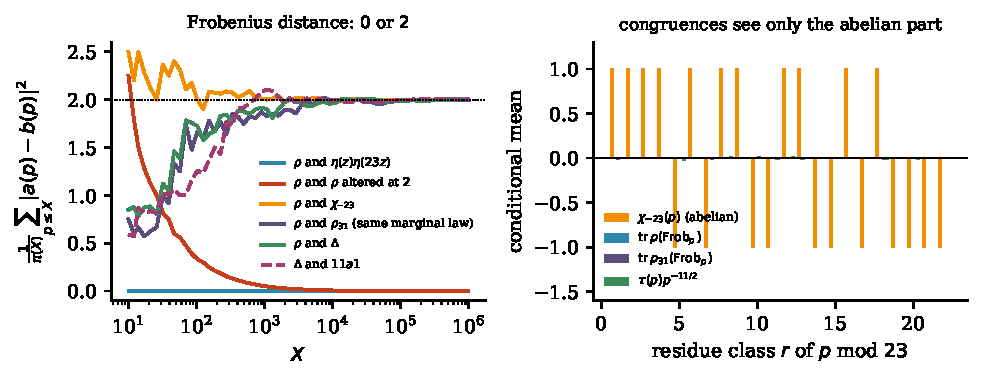
\includegraphics[width=\textwidth]{figs/recip_law.pdf}
\caption{Left: the natural density version $\pi(X)^{-1}\sum_{p\le X}|a(p)-b(p)|^2$ of the squared Frobenius distance. Distinct irreducible or cuspidal objects sit at distance $\sqrt2$ (Theorems~\ref{thm:recipcheb} and \ref{thm:recipcusp}), including $\rho$ and $\rho_{31}$, which have the same marginal law; $\rho$ and $\eta(z)\eta(23z)$ agree at every prime, and $\rho$ altered at $2$ is at distance $0$ from $\rho$ in the limit. Right: means of four Frobenius variables conditional on $p\bmod23$, primes below $10^6$. Only the abelian $\chi_{-23}$ is a function of the residue; the other three are conditionally centred (Proposition~\ref{prop:recipcongruence} for the two Artin traces, Theorem~\ref{thm:recipcusp} with $\pi'$ a Dirichlet character modulo $23$ for $\Delta$).}\label{fig:reciplaw}
\end{figure}

\subsection{Class field theory as measurability}

For $N\ge1$ let $\mathcal F_N$ be the sigma algebra on $\Omega_{S}$ generated by the residue of $p^m$ modulo $N$ (take $S$ to contain the primes dividing $N$). Since $\Frob_p^m$ acts on $\Q(\zeta_N)$ as $\zeta\mapsto\zeta^{p^m}$, $\mathcal F_N$ is generated by the Frobenius class in $\Gal(\Q(\zeta_N)/\Q)$. The conditional law given $\mathcal F_N$ is the probabilistic form of a congruence condition.

\begin{proposition}[congruences see exactly the abelian part; this book, in this form]\label{prop:recipcongruence}\index{Kronecker Weber theorem}
Let $\rho$ be an irreducible Artin representation and $N\ge1$. For every residue $r$ prime to $N$,
\[
\lim_{\sigma\downarrow1}\E_\sigma\bigl[a_\rho\bigm|p^m\equiv r\bmod N\bigr]=\begin{cases}\rho(r)&\text{if }\rho\text{ is inflated from }A_N,\\0&\text{otherwise,}\end{cases}
\]
where $A_N=\Gal(\Q(\zeta_N)/\Q)\cong(\Z/N\Z)^\times$, the first case occurs only when $\dim\rho=1$, and in it $a_\rho$ is itself $\mathcal F_N$ measurable. In particular the Kronecker Weber theorem is equivalent to: every one dimensional Artin representation is $\mathcal F_N$ measurable for some $N$; and no irreducible Artin representation of dimension at least two has a nonzero limiting conditional mean given any congruence.
\end{proposition}

\begin{proof}
Let $K$ be the field cut out by $\rho$ and $\Gamma$ the Galois group of the compositum $L=K(\zeta_N)$, write $A$ for $A_N$, and let $\Gamma_0$ be the subgroup fixing $\Q(\zeta_N)$, so that $A=\Gamma/\Gamma_0$ is abelian. By Theorem~\ref{thm:recipcheb} for $L$, the Frobenius class in $\Gamma$ converges in law to Haar measure, so the conditional mean of $a_\rho$ given that its image in $A$ is $r$ tends to the average of $\chi_\rho$ over the coset $g\Gamma_0$ lying above $r$. Averaging over cosets of $\Gamma_0$ is the orthogonal projection of class functions onto the span of the characters of $A$, so the average equals $\sum_{\psi\in\hat A}\langle\chi_\rho,\psi\rangle_\Gamma\psi(r)$. For irreducible $\rho$ of dimension at least two every $\langle\chi_\rho,\psi\rangle$ vanishes. For one dimensional $\rho$ it is $1$ for $\psi=\rho$ if $\rho$ is inflated from $A$, and $0$ for every $\psi$ otherwise. In the first case $\rho(\Frob_p^m)=\rho(r)$ exactly, which is measurability; here $\rho(r)$ means $\rho$ evaluated at the element $\zeta\mapsto\zeta^r$ of $A_N$.
\end{proof}

This is why reciprocity for $n\ge2$ cannot be a congruence condition, and why it needs automorphic forms: the Hecke eigenvalue $a_\pi(p)$ is the new measurable object that replaces the residue of $p$. Higher conditional moments do see the abelian quotient: for the $S_3$ representation, given $(\frac{p^m}{23})=-1$ the trace is $0$ almost surely, and given $(\frac{p^m}{23})=1$ it is $2$ or $-1$ with limiting conditional probabilities $\frac13,\frac23$, so the limiting conditional mean is $0$ in both cases (Figure~\ref{fig:reciplaw}, right).

\subsection{A dictionary}

\begin{center}\small
\begin{tabular}{p{0.45\textwidth}p{0.45\textwidth}}
\toprule
Arithmetic & Probability\\
\midrule
Frobenius at $p$, Hecke eigenvalue at $p$ & random variables $a_\rho$, $a_\pi$ on $(\Omega_S,\Prob_\sigma)$\\
reciprocity $\rho\leftrightarrow\pi$ & $a_\rho=a_\pi$ almost surely\\
Chebotarev density theorem & convergence in law to Haar measure\\
Schur orthogonality; Rankin Selberg & orthonormality as $\sigma\downarrow1$\\
irreducible Artin; cuspidal & unit second moment; exponential Gamma limit\\
strong multiplicity one & distance zero implies isomorphism\\
class field theory & abelian traces are $\mathcal F_N$ measurable\\
quadratic reciprocity, Gauss's sign & self duality of the normal law\\
functional equation & symmetry of the P\'olya kernel\\
Artin's conjecture and GRH, self dual $\rho$ (Theorem~\ref{thm:recipcm}) & complete monotonicity (Bernstein)\\
converse theorems & a law determined by symmetries of its twists\\
\bottomrule
\end{tabular}
\end{center}

The last line is an analogy rather than a theorem. Twisting by a Dirichlet character is conditioning: since $\mathsf{1}_{p^m\equiv r\bmod N}=\varphi(N)^{-1}\sum_\chi\bar\chi(r)\chi(p^m)$, the twisted series $\sum a(p^m)\chi(p^m)m^{-1}p^{-ms}$ for all $\chi$ modulo $N$ carry the same information as the conditional series given $\mathcal F_N$, and Weil's converse theorem asks for analytic properties of the twists for all moduli in a suitable infinite set, much as the Cram\'er Wold device determines a law on $\R^n$ from its one dimensional projections.

\section{Reciprocity in the Gamma process of a random integer}\label{sec:recipgammaproc}

This section replaces Dirichlet's measure of Section~\ref{sec:reciplaw} by the random integer it comes from, and the random variables by a random measure: label each prime factor of a zeta distributed random integer by its Frobenius class, or by a Satake parameter, and let $\sigma\downarrow1$.

\subsection{The zeta random integer}

For $\sigma>1$ let $N_\sigma=\prod_pp^{e_p}$ be a zeta distributed random integer, $\Prob(N_\sigma=n)=n^{-\sigma}/\zeta(\sigma)$, as in Chapter~\ref{ch:09}, where $e_p$ is written $G_p$. By the compound Poisson form of the geometric law (Exercise~\ref{ex:ch09geometric} of that chapter), $(e_p)_p$ has the law of $(\sum_mmM(p^m))_p$ for independent Poisson variables $M(p^m)$ with means $p^{-m\sigma}/m$, and $\log N_\sigma$ is the zeta subordinator of Proposition~\ref{prop:10dsublaw} at time $1$, with L\'evy measure $\Pi_\sigma$ of Chapter~\ref{ch:10d}.

\begin{lemma}\label{lem:recipzeta}
The exponents $e_p$ are independent and geometric, $\Prob(e_p=k)=(1-p^{-\sigma})p^{-k\sigma}$ for $k\ge0$, and $(\sigma-1)\log N_\sigma$ converges in law to the standard exponential law as $\sigma\downarrow1$.
\end{lemma}

\begin{proof}
The Euler product factorises: for finitely many $t_p$ with $|t_p|\le1$, and $t_p=1$ for the other primes, $\E\prod_pt_p^{e_p}=\zeta(\sigma)^{-1}\prod_p\sum_{k\ge0}t_p^kp^{-k\sigma}=\prod_p(1-p^{-\sigma})/(1-t_pp^{-\sigma})$, a product of geometric generating functions. For the limit, $\E e^{-\lambda(\sigma-1)\log N_\sigma}=\zeta(\sigma+\lambda(\sigma-1))/\zeta(\sigma)\to(1+\lambda)^{-1}$ by the simple pole of $\zeta$ at $1$.
\end{proof}

\subsection{Equidistribution is a Gamma process}

Let $Y$ be a compact metric space, $S$ a finite set of primes, and $(\theta_p)_{p\notin S}$ points of $Y$. We say $(\theta_p)$ is equidistributed with respect to a Borel probability measure $\mu$ on $Y$ if $\pi(t)^{-1}\sum_{p\le t,\,p\notin S}f(\theta_p)\to\int f\,d\mu$ for every continuous $f$. Define the random measure and the marked point process
\[
\Xi_\sigma=\sum_{p\notin S}(\sigma-1)e_p\log p\;\delta_{\theta_p},\qquad \mathcal M_\sigma=\sum_{p\notin S,\,e_p\ge1}\delta_{((\sigma-1)e_p\log p,\;\theta_p)} .
\]
So $\Xi_\sigma$ (a random measure, unrelated to Riemann's $\Xi$ and to the completions $\Xi_\pi$ of Chapter~\ref{ch:10b}) spreads the rescaled logarithm of $N_\sigma$ over the label space, and $\mathcal M_\sigma$ records the rescaled sizes of the prime factors together with their labels. The Gamma random measure $\Gamma_\mu$ with shape measure $\mu$ is the random measure on $Y$ that takes independent values on disjoint Borel sets, with $\Gamma_\mu(B)\sim\mathrm{Gamma}(\mu(B),1)$. Writing $\Gamma_\mu(\lambda)=\int\lambda\,d\Gamma_\mu$, and $\Xi_\sigma(\lambda)$ likewise, its Laplace functional is $\E e^{-\Gamma_\mu(\lambda)}=\exp(-\int\log(1+\lambda)\,d\mu)$ for continuous $\lambda\ge0$, and its atoms form a Poisson process with intensity $x^{-1}e^{-x}dx\,\mu(d\theta)$ \cite{kingman1993}.

\begin{theorem}[equidistribution is a Gamma process; this book]\label{thm:recipgammaproc}
Suppose $(\theta_p)$ is equidistributed with respect to $\mu$. As $\sigma\downarrow1$:
\begin{enumerate}
\item[(i)] $\mathcal M_\sigma$ converges in law, vaguely on $(0,\infty)\times Y$, to the Poisson process with intensity $x^{-1}e^{-x}dx\otimes\mu$: the rescaled sizes of the prime factors of $N_\sigma$ are asymptotically the jumps of a standard Gamma subordinator on $[0,1]$, and their labels are asymptotically independent of the sizes and independent of one another, with law $\mu$;
\item[(ii)] $\Xi_\sigma$ converges in law to $\Gamma_\mu$: for every continuous $\lambda\ge0$ on $Y$, $\E e^{-\Xi_\sigma(\lambda)}\to\exp(-\int_Y\log(1+\lambda)\,d\mu)$.
\end{enumerate}
\end{theorem}

For one point $Y$, part (i) with the sizes normalised by their sum is the Poisson Dirichlet law of the large prime factors of a random integer, due to Billingsley \cite{billingsley1972} for uniform integers; Lloyd \cite{lloyd1984} obtained the limit laws of the largest prime factors of a harmonically distributed integer through the zeta distribution and Poisson variables. Chapter~\ref{ch:pd} develops this: normalised, $\Xi_\sigma$ converges in law to Ferguson's Dirichlet process with base measure $\mu$, and the random integers weighted by the coefficients of the powers of $\zeta$ give the whole Ewens family. The proof of the theorem rests on one estimate.

\begin{lemma}\label{lem:recipnu}
Let $\nu_\sigma=(\sigma-1)\sum_{p\notin S}(\log p)\,p^{-\sigma}\,\delta_{((\sigma-1)\log p,\;\theta_p)}$, a finite measure on $[0,\infty]\times Y$. If $(\theta_p)$ is equidistributed with respect to $\mu$, then $\nu_\sigma$ converges weakly to $e^{-x}dx\otimes\mu$.
\end{lemma}

\begin{proof}
For continuous $f\ge0$ on $Y$ put $A_f(t)=\sum_{p\le t,p\notin S}f(\theta_p)\log p$. Equidistribution and the prime number theorem give $A_f(t)=\mu(f)t+o(t)$ by partial summation, and then the Abelian theorem for Dirichlet series gives
\[
\sum_pf(\theta_p)(\log p)p^{-w}=\frac{\mu(f)}{w-1}+o\Bigl(\frac1{w-1}\Bigr),\qquad w\downarrow1.
\] With $w=\sigma+(\sigma-1)s$, $s\ge0$,
\[
\begin{split}
\int e^{-sx}f(\theta)\,\nu_\sigma(dx,d\theta)&=(\sigma-1)\sum_pf(\theta_p)(\log p)p^{-\sigma-(\sigma-1)s}\\
&\to\frac{\mu(f)}{1+s}=\int_0^\infty e^{-sx}e^{-x}dx\;\mu(f).
\end{split}
\]
By linearity this holds for every continuous $f$. The functions $e^{-sx}f(\theta)$, $s\ge0$, $f\in C(Y)$, span an algebra that contains the constants and separates the points of the compact space $[0,\infty]\times Y$, so it is dense in the continuous functions by Stone and Weierstrass. The total masses converge (take $s=0$, $f=1$), so the convergence extends to all continuous functions.
\end{proof}

\begin{proof}[Proof of Theorem~\ref{thm:recipgammaproc}]
(ii) By Lemma~\ref{lem:recipzeta},
\[
\begin{split}
\log\E e^{-\Xi_\sigma(\lambda)}&=\sum_{p\notin S}\Bigl[\log(1-p^{-\sigma})-\log\bigl(1-p^{-\sigma}e^{-\lambda_pu_p}\bigr)\Bigr]\\
&=-\sum_{p\notin S}p^{-\sigma}\bigl(1-e^{-\lambda_pu_p}\bigr)+R_\sigma ,
\end{split}
\]
where $u_p=(\sigma-1)\log p$, $\lambda_p=\lambda(\theta_p)$ and $R_\sigma=-\sum_{p\notin S}\sum_{m\ge2}m^{-1}p^{-m\sigma}(1-e^{-m\lambda_pu_p})$. Each term of $R_\sigma$ tends to $0$ and is bounded by $p^{-2}$ times a constant, so $R_\sigma\to0$ by dominated convergence. The main term is $-\int h\,d\nu_\sigma$ with $h(x,\theta)=(1-e^{-\lambda(\theta)x})/x$, extended by $\lambda(\theta)$ at $x=0$ and by $0$ at $x=\infty$; $h$ is continuous on $[0,\infty]\times Y$. By Lemma~\ref{lem:recipnu} and Frullani's integral,
\[
\int h\,d\nu_\sigma\to\int_Y\!\int_0^\infty\frac{1-e^{-\lambda(\theta)x}}x\,e^{-x}dx\,\mu(d\theta)=\int_Y\log(1+\lambda)\,d\mu .
\]
(i) Let $F\ge0$ be continuous with compact support in $(0,\infty)\times Y$, say in $[a,b]\times Y$ with $a>0$. Then $-\log\E e^{-\mathcal M_\sigma(F)}=-\sum_p\log(1-y_p)$ with $y_p=\sum_{k\ge1}\Prob(e_p=k)(1-e^{-F(ku_p,\theta_p)})$. The terms with $k\ge2$ contribute at most $\sum_p\sum_{k\ge2}p^{-k}\mathsf{1}\{ku_p\ge a\}$, which tends to $0$ by dominated convergence, and $\sum_py_p^2\to0$ in the same way; replacing $\Prob(e_p=1)$ by $p^{-\sigma}$ costs at most $\sum_pp^{-2}\mathsf{1}\{u_p\ge a\}\to0$, so
\[
-\log\E e^{-\mathcal M_\sigma(F)}=\sum_pp^{-\sigma}(1-e^{-F(u_p,\theta_p)})+o(1)=\int g\,d\nu_\sigma+o(1)
\]
with $g=(1-e^{-F})/x$, which is continuous on $[0,\infty]\times Y$ because $F$ vanishes near $x=0$. Lemma~\ref{lem:recipnu} gives the limit $\int(1-e^{-F})x^{-1}e^{-x}dx\,d\mu$, the Laplace functional of the Poisson process.
\end{proof}

The hypothesis holds for the following label sequences. For a finite Galois extension $K/\Q$ with group $G$, $\theta_p$ is the class $\Frob_p$ in the set $G^\natural$ of conjugacy classes and $\mu=\mu_G$ is the image of Haar measure, by Chebotarev's theorem in its natural density form (Corollary~\ref{cor:ch3cheb}) \cite{chebotarev1926}. For a holomorphic newform of weight $k\ge2$ with trivial character and without complex multiplication, $\theta_p\in[0,\pi]$ is the angle with $x_p=a_p/p^{(k-1)/2}=2\cos\theta_p$, and $\mu$ is the Sato Tate law $\frac2\pi\sin^2\theta\,d\theta$, whose image under $\theta\mapsto2\cos\theta$ is $\ST$, by Theorem~\ref{thm:01satotate} \cite{blght2011}. For two elliptic curves over $\Q$ without complex multiplication and not geometrically isogenous, $\theta_p$ is the pair of angles and $\mu$ the product of two Sato Tate laws, by Theorem~\ref{thm:04joint} \cite{harris2009}.

\begin{corollary}[Chebotarev as a Gamma process; this book]\label{cor:recipchebgamma}
Let $K/\Q$ be finite Galois with group $G$, unramified outside $S$, and for a conjugacy class $C$ let $L_C(\sigma)=(\sigma-1)\sum_{p\notin S,\,\Frob_p\in C}e_p\log p$ be the rescaled part of $\log N_\sigma$ carried by primes with Frobenius in $C$. As $\sigma\downarrow1$:
\begin{enumerate}
\item[(i)] the $L_C(\sigma)$, $C\in G^\natural$, are independent for every $\sigma$, and $L_C(\sigma)$ converges in law to $\mathrm{Gamma}(|C|/|G|,1)$;
\item[(ii)] the shares $L_C/\sum_{C'}L_{C'}$ have a Dirichlet limit law with parameters $(|C|/|G|)_C$, independent of the total, which is standard exponential;
\item[(iii)] for a quadratic character $\chi$, the share of $\log N_\sigma$ carried by the primes with $\chi(p)=-1$ converges to the arcsine law $\pi^{-1}(u(1-u))^{-1/2}du$ on $(0,1)$.
\end{enumerate}
\end{corollary}

\begin{proof}
(i) The $L_C(\sigma)$ depend on disjoint sets of the independent $e_p$, and the limit is Theorem~\ref{thm:recipgammaproc}(ii) on the finite space $G^\natural$, with $\lambda$ a function of the class. (ii) is the beta gamma algebra (independent gamma variables normalised by their sum are Dirichlet and independent of the sum) and the continuous mapping theorem, the total being positive almost surely. (iii) is (ii) for $G=\{\pm1\}$, where the Dirichlet law is $\mathrm{Beta}(\frac12,\frac12)$.
\end{proof}

The mean of the share in (ii) is $|C|/|G|$, which is Chebotarev's density. What the Gamma process adds is the fluctuation: the share does not concentrate, because $\log N_\sigma$ is dominated by a few large prime factors, and their labels are independent Haar samples. In the language of Chapter~\ref{ch:pd}, the limit shares are the masses of the classes under a Dirichlet process with base measure $\mu$, the limit of the normalised labelled factorisation (Theorem~\ref{thm:pddirichlet}). Part (iii) is an arithmetic arcsine law, in the same sense as L\'evy's arcsine law for the time Brownian motion spends positive: a Gamma subordinator split into two halves of equal intensity.

For the $S_3$ field of $x^3-x-1$, ramified only at $23$ (Example~\ref{ex:ch3cubic}; Figure~\ref{fig:ch03_chebotarev} shows its Chebotarev frequencies in natural density), the Laplace transforms $\E e^{-\lambda L_C(\sigma)}$ were computed from the Euler product over the primes below $10^7$, with the remaining primes accounted for by the prime number theorem. Figure~\ref{fig:recipgammaproc}, left, shows them converging to $(1+\lambda)^{-1/6}$, $(1+\lambda)^{-1/2}$ and $(1+\lambda)^{-1/3}$ for the identity class, the transpositions and the three cycles. At $\lambda=1$ the transform differs from its limit by a factor of about $1+\kappa_C(\sigma-1)$, with $\kappa_C$ between $0.38$ and $1.07$ (Theorem~\ref{thm:recipdrift}).

\begin{figure}[t]
\centering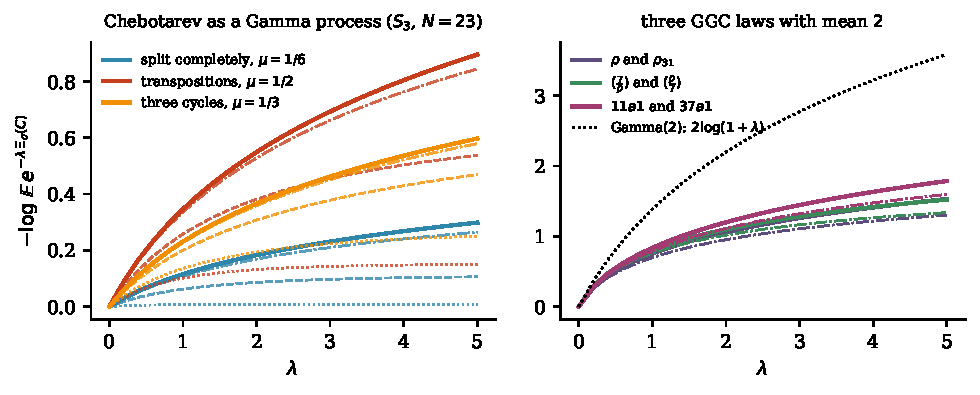
\includegraphics[width=\textwidth]{figs/recip_gammaproc.pdf}
\caption{Left: Corollary~\ref{cor:recipchebgamma} for the $S_3$ field of $x^3-x-1$. Laplace exponents of $L_C(\sigma)=\Xi_\sigma(C)$, from Euler products over $p<10^7$ with a prime number theorem tail, for $\sigma=1.5$ (dotted), $1.1$ (dashed) and $1.01$ (dash dotted) against the Gamma limits $\mu(C)\log(1+\lambda)$. Right: three GGC limits from Theorems~\ref{thm:recipggcfun} and \ref{thm:recipthorin}, all with mean $2$ and with different Thorin measures, against the Gamma$(2)$ limit of the intensity scaling of Theorem~\ref{thm:recipzerotwo}; dash dotted curves are $\sigma=1.01$.}\label{fig:recipgammaproc}
\end{figure}

\subsection{Frobenius functionals are generalized gamma convolutions}

Recall from Definition~\ref{def:ch10ggc} that a GGC is a law on $[0,\infty)$ with Laplace transform
\[
\exp\Bigl(-a\lambda-\int_{(0,\infty)}\log(1+\lambda/t)\,\tau(dt)\Bigr),\qquad\lambda\ge0,
\]
where $a\ge0$ is the drift and $\tau$ the Thorin measure \cite{thorin1977,bondesson1992}. Its mean is $a+\int t^{-1}\,\tau(dt)$, and we call $\tau((0,\infty))$ its Thorin mass. We write $\mathrm{Gamma}(\alpha)$ for the gamma law of shape $\alpha$ and rate $1$, whose Thorin measure is $\alpha\delta_1$, with $\mathrm{Gamma}(0)=\delta_0$.

\begin{theorem}[Frobenius functionals are GGCs; this book]\label{thm:recipggcfun}
Suppose $(\theta_p)$ is equidistributed with respect to $\mu$ and let $Q\ge0$ be continuous on $Y$. Then
\[
\Xi_\sigma(Q)=(\sigma-1)\sum_{p\notin S}e_p\log p\;Q(\theta_p)
\]
converges in law to a GGC with drift zero and Thorin measure $\tau_Q$, the image of $\mu$ restricted to $\{Q>0\}$ under $\theta\mapsto1/Q(\theta)$. Its mean is $\int Q\,d\mu$ and its Thorin mass is $\mu(Q>0)$. Moreover, if $\{Q>0\}$ is a $\mu$ continuity set,
\[
\log\Prob\bigl(\Xi_\sigma(Q)=0\bigr)=-\mu(Q>0)\log\frac1{\sigma-1}+o\Bigl(\log\frac1{\sigma-1}\Bigr).
\]
\end{theorem}

\begin{proof}
Apply Theorem~\ref{thm:recipgammaproc}(ii) to $\lambda Q$: the limit Laplace transform is
\[
\exp\Bigl(-\int\log(1+\lambda Q)\,d\mu\Bigr)=\exp\Bigl(-\int_{\{Q>0\}}\log\bigl(1+\lambda/(1/Q)\bigr)\,d\mu\Bigr),
\]
which is the GGC transform with Thorin measure $\tau_Q$. The mean is $\int t^{-1}\tau_Q(dt)$, which is $\int Q\,d\mu$. For the last statement, $\Xi_\sigma(Q)=0$ exactly when $e_p=0$ for every $p$ with $Q(\theta_p)>0$, so
\[
\log\Prob(\Xi_\sigma(Q)=0)=\sum_{Q(\theta_p)>0}\log(1-p^{-\sigma})=-\sum_{Q(\theta_p)>0}p^{-\sigma}+O(1),
\]
and equidistribution on the continuity set $\{Q>0\}$ gives $\sum_{Q(\theta_p)>0}p^{-\sigma}\sim\mu(Q>0)\log\frac1{\sigma-1}$ by partial summation.
\end{proof}

So the Thorin mass is visible as an exponent, and for Chebotarev labels, where the error term is $O(1)$ by Lemma~\ref{lem:recipvirtual}, the probability that no prime factor of $N_\sigma$ has a label where $Q>0$ is of exact order $(\sigma-1)^{\mu(Q>0)}$. Figure~\ref{fig:recipzero}, left, shows the fitted slopes $0.608$, $0.497$ and $0.989$, against Thorin masses $\frac{11}{18}$, $\frac12$ and $1$ for the three examples of the next section. For $Q=\mathsf 1_C$ Chapter~\ref{ch:pd} computes the constant of this order, and its counterpart for uniform random integers, a case of Serre's theorem on frobenian sets (Theorem~\ref{thm:pdrate}).

\subsection{Reciprocity as vanishing of a Thorin measure}

We now take $Q$ to be a squared discrepancy between two kinds of Frobenius data. The limit is $\delta_0$ exactly when $\tau_Q$ vanishes, so reciprocity laws become vanishing statements, and their failures have computable Thorin measures.

\begin{theorem}[Thorin criteria for reciprocity; this book]\label{thm:recipthorin}
In each case $S$ contains the primes at which the data are ramified (in (b) those ramified in $K(\zeta_N)$, in (c) $2$ and $q$, in (d) the primes of bad reduction of $E$ and $E'$), and $\Xi_\sigma(Q)$ converges in law to the GGC with Thorin measure $\tau_Q$ of Theorem~\ref{thm:recipggcfun}.
\begin{enumerate}
\item[(a)] Artin representations. Let $\rho,\rho'$ be Artin representations unramified outside $S$, with fields $K,K'$ (the fixed fields of their kernels), and put $H=\Gal(KK'/\Q)$ and $Q=|\chi_\rho-\chi_{\rho'}|^2$ on $H^\natural$. Then $\tau_Q$ is the image of Haar probability measure on $\{\chi_\rho\ne\chi_{\rho'}\}\subset H$ under $1/|\chi_\rho-\chi_{\rho'}|^2$. The limit law has mean $\|\chi_\rho-\chi_{\rho'}\|^2_{L^2(H)}$, which is $2$ for nonisomorphic irreducible $\rho,\rho'$, and $\tau_Q=0$ if and only if $\rho\cong\rho'$.
\item[(b)] Abelian reciprocity. Let $\psi$ be a character of finite order of $\Gal(\overline\Q/\Q)$, $\chi$ a Dirichlet character modulo $N$, and $Q=|\psi(\Frob_p)-\chi(p)|^2$. If $\psi\ne\chi$ as characters of $\Gal(K(\zeta_N)/\Q)$, where $K$ is the field of $\psi$, and $\psi\bar\chi$ has order $d$, then
\[
\tau_Q=\frac1d\sum_{j=1}^{d-1}\delta_{1/(4\sin^2(\pi j/d))},
\]
and the limit law has mean $2$ and Thorin mass $1-\frac1d$; otherwise $\tau_Q=0$. The Kronecker Weber theorem is equivalent to the statement that for every $\psi$ there are $N$ and $\chi$ with $\tau_Q=0$.
\item[(c)] Quadratic reciprocity. Let $q\equiv3\bmod4$ be prime. For $Q=|(\frac qp)-(\frac pq)|^2$ the limit law is the gamma law of shape $\frac12$ and rate $\frac14$, that is $2\chi^2_1$, with Thorin measure $\frac12\delta_{1/4}$; for $Q=|(\frac qp)-(\frac pq)(\frac{-1}p)|^2$ the limit is $\delta_0$. For $q\equiv1\bmod4$ the first $Q$ already gives $\delta_0$.
\item[(d)] Elliptic curves. Let $E,E'$ be elliptic curves over $\Q$ without complex multiplication and not geometrically isogenous, with normalised traces $x_p,x'_p$, and $Q=(x_p-x'_p)^2$. Then $\tau_Q$ is the law of $1/(X-X')^2$ for independent $X,X'$ with law $\ST$, so the Thorin mass is $1$ and the limit law has mean $2$. If instead $E'$ is isogenous to $E$, then $Q=0$ for all good $p$ and the limit is $\delta_0$.
\end{enumerate}
\end{theorem}

\begin{proof}
(a) Chebotarev for $KK'$ gives equidistribution of $\Frob_p$ in $H^\natural$ with respect to Haar measure, and Theorem~\ref{thm:recipggcfun} applies with $Y=H^\natural$. The mean is $\int|\chi_\rho-\chi_{\rho'}|^2$; it is $\langle\chi_\rho,\chi_\rho\rangle+\langle\chi_{\rho'},\chi_{\rho'}\rangle-2\operatorname{Re}\langle\chi_\rho,\chi_{\rho'}\rangle=2$ for nonisomorphic irreducibles. Every class of the finite group $H$ has positive Haar measure, so $\tau_Q=0$ forces $\chi_\rho=\chi_{\rho'}$ on $H$, hence $\rho\cong\rho'$.

(b) Here $\psi$ and $\chi$ are both characters of $G_N=\Gal(K(\zeta_N)/\Q)$, $\chi$ through the cyclotomic identification $\Frob_p\mapsto p\bmod N$. Then $Q(g)=|1-(\psi\bar\chi)(g)|^2$. If $\psi\bar\chi$ is nontrivial of order $d$, its values are equidistributed over the $d$th roots of unity under Haar measure on $G_N$, and $|1-e^{2\pi ij/d}|^2=4\sin^2(\pi j/d)$. The mean is $\frac1d\sum_j4\sin^2(\pi j/d)=2$. If $\psi\bar\chi$ is trivial, $Q$ vanishes identically. Kronecker Weber says every $\psi$ factors through some $\Gal(\Q(\zeta_N)/\Q)$, which is the existence of $\chi$ with $\psi=\chi$ on $G_N$; conversely $\tau_Q=0$ gives $\psi=\chi$ on $G_N$.

(c) For odd $p\ne q$, $(\frac qp)$ is the Frobenius character of $\Q(\sqrt q)$, and the law of quadratic reciprocity is $(\frac qp)=(\frac pq)(\frac{-1}p)^{(q-1)/2}$. So for $q\equiv3\bmod4$ the character $\psi\bar\chi$ in (b) is $(\frac{-1}{\cdot})$, of order $d=2$, and $\tau_Q=\frac12\delta_{1/4}$, whose GGC is $(1+4\lambda)^{-1/2}$, the transform of $2\chi^2_1$.

(d) Theorem~\ref{thm:04joint} gives equidistribution of $(x_p,x'_p)$ with respect to $\ST\otimes\ST$, and the diagonal has measure zero, so the mass is $1$; the mean is $\E(X-X')^2=2$. For isogenous curves $a_p=a'_p$ for all good $p$.
\end{proof}

Parts (b) and (c) restate Kronecker Weber and quadratic reciprocity rather than reprove them, since the vanishing of $\tau_Q$ is equivalent to the equality of two characters; what is new is the shape of failure. A mismatched abelian reciprocity is a GGC whose Thorin atoms $1/(4\sin^2(\pi j/d))$ are reciprocals of the squared sines of the $2\sin^2$ lemma (Lemma~\ref{lem:10dsin2}), and omitting the sign factor $(\frac{-1}p)$ from quadratic reciprocity leaves precisely a scaled chi squared variable with one degree of freedom. Numerically (Figure~\ref{fig:recipgammaproc}, right), the three examples $(\rho,\rho_{31})$, $((\frac7p),(\frac p7))$ and $(11a1,37a1)$ all have mean $2$ and different limit laws: orthonormality fixes the mean, and the Thorin measure records the law of the squared discrepancy $Q$, which depends on the joint law of the two kinds of Frobenius data.

\begin{figure}[t]
\centering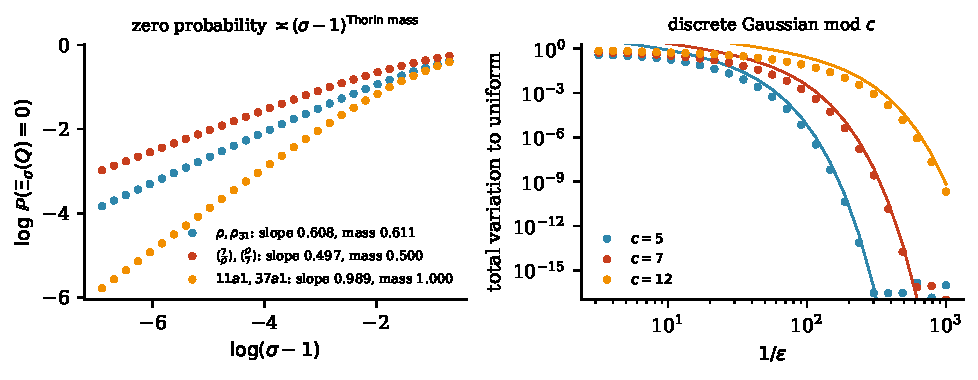
\includegraphics[width=\textwidth]{figs/recip_zeroheat.pdf}
\caption{Left: Theorem~\ref{thm:recipggcfun}. The probability that no prime factor of $N_\sigma$ has a label where $Q>0$, computed from the Euler product over primes below $10^7$ with a prime number theorem tail, decays like $(\sigma-1)^m$, with $m$ the Thorin mass. Right: Theorem~\ref{thm:recipheat}. Total variation distance between a discrete Gaussian with parameter $\varepsilon$ reduced modulo $c$ and the uniform law (dots), against the bound of part (i) (lines). For $c=5$ and $7$ the dots that level off near $10^{-16}$, above the lines, are rounding errors of the double precision computation, not distances.}\label{fig:recipzero}
\end{figure}

\subsection{A second scaling and a zero two law}

Theorem~\ref{thm:recipggcfun} uses $Q$ as a mark on the jumps of a fixed random integer. One can instead let $Q$ change the intensity: take two of the Frobenius variables $a,b$ of Section~\ref{sec:reciplaw} (each an $a_\rho$ or an $a_\pi$, fixed in the next theorem), put $Q_m(p)=|a(p^m)-b(p^m)|^2\ge0$, and replace the zeta integer by the random integer $N_{Q,\sigma}$ with $\Prob(N_{Q,\sigma}=n)\propto d_Q(n)n^{-\sigma}$, where $\sum_nd_Q(n)n^{-s}=D_Q(s)$ is the Dirichlet series with $\log D_Q(s)=\sum_{p\notin S,m}Q_m(p)m^{-1}p^{-ms}$. Its logarithm $X_\sigma=\log N_{Q,\sigma}$ is the discrepancy subordinator; for $b=0$ it is the Rankin Selberg subordinator of Theorem~\ref{thm:recipgamma}, which is the case $\rho'=0$ of the next theorem.

\begin{theorem}[zero two law; this book]\label{thm:recipzerotwo}
(a) For Artin representations $\rho,\rho'$ with $a=\tr\rho$, $b=\tr\rho'$, $(\sigma-1)X_\sigma$ converges in law to $\mathrm{Gamma}(\|\chi_\rho-\chi_{\rho'}\|^2)$, a GGC with Thorin measure $\|\chi_\rho-\chi_{\rho'}\|^2\delta_1$ and integer shape; for irreducible $\rho,\rho'$ the shape is $0$ or $2$.
(b) For unitary cuspidal automorphic representations $\pi,\pi'$ of $\GL_n(\A_\Q)$, $\GL_{n'}(\A_\Q)$ with $a=a_\pi$, $b=a_{\pi'}$, the limit is $\delta_0$ if $\pi\cong\pi'$ and $\mathrm{Gamma}(2)$ otherwise.
\end{theorem}

\begin{proof}
$D_Q=L(\rho\otimes\check\rho)L(\rho'\otimes\check\rho')/(L(\rho\otimes\check\rho')L(\rho'\otimes\check\rho))$ up to finitely many Euler factors, the $L$ function of the virtual character $|\chi_\rho-\chi_{\rho'}|^2$. By Lemma~\ref{lem:recipvirtual} it has a pole of order $e=\langle|\chi_\rho-\chi_{\rho'}|^2,1\rangle=\|\chi_\rho-\chi_{\rho'}\|^2$ at $s=1$ and is otherwise holomorphic and nonzero near $1$, so $\E e^{-\lambda(\sigma-1)X_\sigma}=D_Q(\sigma+\lambda(\sigma-1))/D_Q(\sigma)\to(1+\lambda)^{-e}$. For (b), the same computation with $L(s,\pi\times\tilde\pi')$, which by Jacquet, Shalika, Moeglin, Waldspurger and Shahidi \cite{jacquetshalika1981,moeglinwaldspurger1989,shahidi1981} has a simple pole at $1$ exactly when $\pi'\cong\pi$ and no zero on $\operatorname{Re}s=1$, gives $e=2-2\delta_{\pi\cong\pi'}$.
\end{proof}

The two scalings give two GGCs with the same mean $\int Q\,d\mu$: in Theorem~\ref{thm:recipzerotwo} the Thorin measure $\tau_Q$ of Theorem~\ref{thm:recipggcfun} collapses to a single atom at $1$ carrying the mean. Integrality of the collapsed shape is Schur orthogonality, and the value $2$ for distinct irreducibles is the orthonormality of characters; for cuspidal pairs it is Rankin Selberg. The natural extension to the mixed case is the following conjecture.

\begin{conjecture}[mixed zero two law]\label{conj:recipmixed}
Let $\rho$ be an irreducible Artin representation of dimension $n$ and $\pi$ a unitary cuspidal automorphic representation of $\GL_n(\A_\Q)$, with $a=\tr\rho$ and $b=a_\pi$. Then $(\sigma-1)X_\sigma$ converges in law to $\delta_0$ or to $\mathrm{Gamma}(2)$, and to $\delta_0$ exactly when $L(s,\rho_p)=L(s,\pi_p)$ for almost all $p$.
\end{conjecture}

\begin{proposition}[this book]\label{prop:recipmixed}
(i) If $\rho$ is automorphic, Conjecture~\ref{conj:recipmixed} holds for $\rho$ and every $\pi$. Hence it holds for $n=1$, for odd two dimensional $\rho$, and for two dimensional $\rho$ with solvable image.
(ii) Unconditionally, $\limsup_{\sigma\downarrow1}\E[(\sigma-1)X_\sigma]\le4$ and $\E[((\sigma-1)X_\sigma)^2]$ stays bounded, so under the conjecture $\E[(\sigma-1)X_\sigma]$ tends to $0$ or $2$.
(iii) If the limit is $\delta_0$ then $\rho$ and $\pi$ are reciprocal in law, so $\pi$ is unique up to isomorphism and, for every $\epsilon>0$, $|a_\rho(p)-a_\pi(p)|\le\epsilon$ outside a set of primes of Dirichlet density zero (Corollary~\ref{cor:reciplaw}(ii) and (iv)).
\end{proposition}

\begin{proof}
(i) If $\rho$ corresponds to $\pi_\rho$, then $a=a_{\pi_\rho}$ off a finite set and Theorem~\ref{thm:recipzerotwo}(b) applies to $(\pi_\rho,\pi)$. The listed cases are class field theory, Khare and Wintenberger \cite{kharewintenberger2009,kharewintenberger2009b} with work of Kisin \cite{kisin2009}, and Langlands and Tunnell \cite{langlands1980,tunnell1981}. (ii) The mean is $(\sigma-1)\sum_{p,m}Q_m(p)(\log p)p^{-m\sigma}$. Since $Q_m\le2|a(p^m)|^2+2|b(p^m)|^2$, it is at most $2(\sigma-1)(-L'/L)(\sigma,\rho\otimes\check\rho)+2(\sigma-1)(-L'/L)(\sigma,\pi\times\tilde\pi)$ up to finitely many Euler factors, and both terms tend to $2$ because each $L$ function has a simple pole at $1$. The same bound for $(\log D_Q)''(\sigma)$, the variance of $X_\sigma$, gives $\operatorname{Var}((\sigma-1)X_\sigma)\le4+o(1)$, since $(\sigma-1)^2(\log L)''(\sigma)\to1$ at a simple pole; so $\E[((\sigma-1)X_\sigma)^2]\le20+o(1)$, and the means converge whenever the laws do. (iii) Put
\[
\eta_\sigma=(\sigma-1)\sum_{p,m}Q_m(p)(\log p)p^{-m\sigma}\delta_{(\sigma-1)m\log p}.
\]
The Laplace exponent at $\lambda=1$ is
\[
\int\frac{1-e^{-x}}x\,\eta_\sigma(dx)\ge\frac{1-e^{-K}}K\,\eta_\sigma([0,K]),
\]
so $\eta_\sigma([0,K])\to0$ for every $K$; the tails $\eta_\sigma([K,\infty))$ are at most $4e^{-K}+o(1)$ by the same bound as in (ii) applied to the Gamma limits of $|a|^2$ and $|b|^2$. Hence $(\sigma-1)\sum Q_m(p)(\log p)p^{-m\sigma}\to0$, and integrating in $\sigma$, $\log D_Q(\sigma)=\int_\sigma^2\sum Q_m(p)(\log p)p^{-mw}dw+O(1)=o(\log\frac1{\sigma-1})$, which is the definition of reciprocity in law.
\end{proof}

Conjecture~\ref{conj:recipmixed} follows from reciprocity (Proposition~\ref{prop:recipmixed}(i)) but does not imply it, because it asserts no existence: for a nonautomorphic $\rho$ it predicts the limit $\mathrm{Gamma}(2)$ for every $\pi$. It is the orthogonality half of reciprocity, and existence is the other half: by its last clause, reciprocity for $\rho$ is equivalent to the conjecture together with the existence of one $\pi$ whose limit is $\delta_0$. If $L(s,\rho_p)=L(s,\pi_p)$ for almost all $p$, then $Q_m(p)=0$ outside a finite set of primes and the limit is $\delta_0$ unconditionally; conversely, without the conjecture, a $\delta_0$ limit makes $\rho$ and $\pi$ reciprocal in law (Proposition~\ref{prop:recipmixed}(iii)), and whether that forces $a_\rho(p)=a_\pi(p)$ for all but finitely many $p$ is Open Problem~\ref{op:reciplaw}.

\subsection{Second order Chebotarev: the Euler Kronecker drift}

The Gamma limit of Corollary~\ref{cor:recipchebgamma} is approached at rate $\sigma-1$ (Figure~\ref{fig:recipdrift}), with a constant given by logarithmic derivatives of Artin $L$ functions at $s=1$ and a prime power term.

For a character $\chi$ of $G=\Gal(K/\Q)$ and the finite set $S$ put
\[
\gamma^S(\chi)=\lim_{s\to1}\Bigl(\frac{(L^S)'}{L^S}(s,\chi)+\frac{\delta_{\chi=1}}{s-1}\Bigr),
\]
where $L^S$ omits the Euler factors at $S$. For $\chi\ne1$ this is
\[
\frac{L'}L(1,\chi)+\sum_{p\in S}\sum_{m\ge1}\tr(\Frob_p^m\mid V_\chi^{I_p})\,(\log p)\,p^{-m},
\]
where $V_\chi$ is a representation with character $\chi$ and $I_p$ an inertia group at $p$, and for $\chi=1$ it is $\gamma_{\mathrm E}+\sum_{p\in S}\frac{\log p}{p-1}$ with $\gamma_{\mathrm E}$ Euler's constant. The Euler Kronecker constant of $K$ in Ihara's sense \cite{ihara2006} is
\[
\gamma_K=\lim_{s\to1}\Bigl(\frac{\zeta_K'}{\zeta_K}(s)+\frac1{s-1}\Bigr)=\sum_\chi\chi(1)\gamma^\emptyset(\chi),
\]
and $\gamma_K^S$ denotes the same constant for $\zeta_K$ with the Euler factors above $S$ removed.

\begin{theorem}[Euler Kronecker drift; this book]\label{thm:recipdrift}
Let $K/\Q$ be finite Galois with group $G$, unramified outside $S$, and $C$ a conjugacy class. Uniformly for $\lambda$ in compact subsets of $[0,\infty)$,
\[
\log\E e^{-\lambda L_C(\sigma)}=-\mu(C)\log(1+\lambda)+\kappa_C\,\lambda\,(\sigma-1)+O\bigl((\sigma-1)^2\bigr),
\]
with
\[
\kappa_C=\mu(C)\sum_\chi\overline{\chi(C)}\,\gamma^S(\chi)\;-\;\sum_{p\notin S}\sum_{m\ge2}\bigl[\mathsf 1_C(\Frob_p)-\mathsf 1_C(\Frob_p^m)\bigr]\,(\log p)\,p^{-m},
\]
the sum over irreducible characters. In particular $\E L_C(\sigma)=\mu(C)-\kappa_C(\sigma-1)+O((\sigma-1)^2)$: to first order the Gamma limit is shifted by the deterministic amount $-\kappa_C(\sigma-1)$. For the class of primes that split completely,
\[
\kappa_{\{1\}}=\frac{\gamma_K^S}{|G|}+\sum_{p\notin S,\;\Frob_p\ne1}\;\sum_{m\ge2,\;\Frob_p^m=1}(\log p)\,p^{-m},
\]
the Euler Kronecker constant of $K$ with the Euler factors above $S$ removed, divided by the degree, plus a nonnegative prime power term. For a class function $Q\ge0$, independence of the $L_C(\sigma)$ gives $\log\E e^{-\lambda\Xi_\sigma(Q)}=-\sum_C\mu(C)\log(1+\lambda Q_C)+\kappa_Q\lambda(\sigma-1)+O((\sigma-1)^2)$ with $\kappa_Q=\sum_CQ_C\,\kappa_C$.
\end{theorem}

\begin{proof}
By Lemma~\ref{lem:recipzeta}, $\log\E e^{-\lambda L_C(\sigma)}=P_C(\sigma')-P_C(\sigma)$ with $\sigma'=\sigma+\lambda(\sigma-1)$ and $P_C(s)=\sum_{p\notin S,\Frob_p\in C}\sum_mm^{-1}p^{-ms}$. Expand $\mathsf 1_C=\sum_\chi c_\chi\chi$ with $c_\chi=\mu(C)\overline{\chi(C)}$. Since $\sum_\chi c_\chi\chi(g^m)=\mathsf 1_C(g^m)$,
\[
\sum_\chi c_\chi\log L^S(s,\chi)=\sum_{p\notin S}\sum_m\frac{\mathsf 1_C(\Frob_p^m)}{m\,p^{ms}},
\]
so that
\[
P_C(s)=\sum_\chi c_\chi\log L^S(s,\chi)+R_C(s),
\]
with
\[
R_C(s)=\sum_{p\notin S}\sum_{m\ge2}\bigl[\mathsf 1_C(\Frob_p)-\mathsf 1_C(\Frob_p^m)\bigr]m^{-1}p^{-ms}
\]
holomorphic on $\operatorname{Re}s>\frac12$. By Brauer's theorem each $L^S(s,\chi)$, $\chi\ne1$, is holomorphic and nonzero near $s=1$, and $(s-1)\zeta^S(s)$ is too. So $h_C(s)=P_C(s)-\mu(C)\log\frac1{s-1}$ is real analytic near $s=1$, with $h_C'(1)=\sum_\chi c_\chi\gamma^S(\chi)+R_C'(1)=\kappa_C$. Then $P_C(\sigma')-P_C(\sigma)=-\mu(C)\log(1+\lambda)+h_C(\sigma')-h_C(\sigma)$, and Taylor's theorem gives the expansion. The mean is minus the derivative in $\lambda$ at $0$. For $C=\{1\}$, $c_\chi=\chi(1)/|G|$ and $\sum_\chi\chi(1)\gamma^S(\chi)=\gamma_K^S$ because $\zeta_K^S=\prod_\chi L^S(s,\chi)^{\chi(1)}$; the prime power term is nonnegative because a power of the identity is the identity. The statement for $Q$ follows by summing over classes.
\end{proof}

For the $S_3$ field of $x^3-x-1$ the set $S$ consists of $2$, $7$, $11$, $23$, $31$ and $37$, the primes that are bad for some example of this section. PARI/GP gives $\frac{L'}L(1,\chi_{-23})=-0.42212$ and $\frac{L'}L(1,\rho)=1.01706$, so $\gamma_K=\gamma_{\mathrm E}-0.42212+2(1.01706)=2.18922$; with the Euler factors above $S$ removed, $\gamma_K^S=3.59058$, and the prime power term of Theorem~\ref{thm:recipdrift} is $0.14171$, so $\kappa_{\{1\}}=3.59058/6+0.14171=0.74014$. Theorem~\ref{thm:recipdrift} predicts the drifts in the first row below; the second row is the intercept of a linear fit of $[\log\E e^{-L_C(\sigma)}+\mu(C)\log2]/(\sigma-1)$ over $\sigma-1\in[0.00125,0.04]$ (for $Q$, with $\frac12\log5$ in place of $\mu(C)\log2$), from the Euler products used for Figure~\ref{fig:recipgammaproc} (Figure~\ref{fig:recipdrift}).
\begin{center}\small
\begin{tabular}{lcccc}
\toprule
& identity & transpositions & three cycles & $Q=|(\frac7p)-(\frac p7)|^2$\\
\midrule
$\kappa$ predicted & $0.74014$ & $1.07416$ & $0.37746$ & $4.4189$\\
fitted & $0.73881$ & $1.07365$ & $0.37710$ & $4.4058$\\
\bottomrule
\end{tabular}
\end{center}
The three class drifts add up to $\gamma_{\mathrm E}+\sum_{p\in S}\frac{\log p}{p-1}=2.19176$, the drift of $(\sigma-1)\sum_{p\notin S}e_p\log p$, the part of $(\sigma-1)\log N_\sigma$ carried by the primes outside $S$; for $(\sigma-1)\log N_\sigma$ itself the drift is $\gamma_{\mathrm E}$. The prime power term of $\kappa_C$ is the Dirichlet density counterpart of the prime square bias that Section~\ref{sec:ch3cheb} measures for the same field. For uniform random integers below $x$, with $S$ the set of ramified primes, a size biased prime factor has Frobenius in $C$ with probability $\mu(C)+(\gamma_{\mathrm E}\mu(C)-\kappa_C)/(\log x-1)+O((\log x)^{-2})$ (Theorem~\ref{thm:pdmertens}).

\begin{figure}[t]
\centering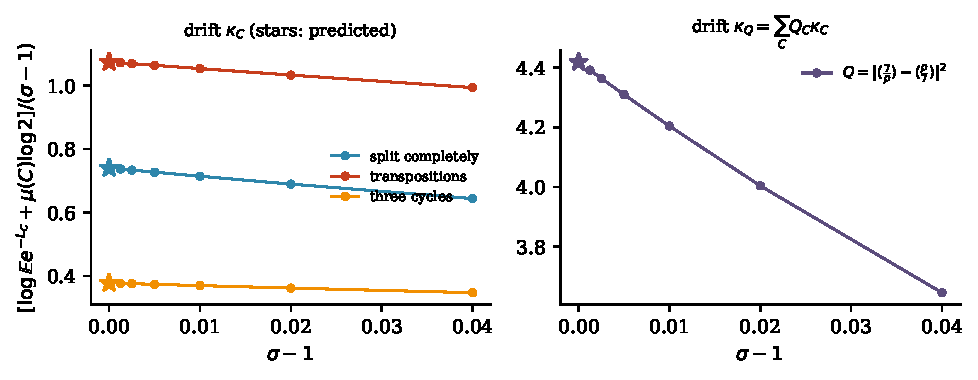
\includegraphics[width=\textwidth]{figs/recip_drift.pdf}
\caption{Theorem~\ref{thm:recipdrift}. The normalised deviation of the logarithm of the Laplace transform from its Gamma limit, at $\lambda=1$, as $\sigma\downarrow1$, for the three classes of the $S_3$ field (left) and for the quadratic reciprocity discrepancy with the sign factor omitted (right). Stars are the predicted drifts.}\label{fig:recipdrift}
\end{figure}

Under GRH Ihara showed that $\gamma_K$ is at most about $2\log\log\sqrt{|d_K|}$ \cite{ihara2006}. Since $(\gamma_K^S-\gamma_K)/|G|\le\sum_{p\in S}\frac{\log p}{p-1}$ and the prime power term is at most $\sum_p\frac{\log p}{p(p-1)}<0.76$, GRH bounds the drift of the split class from above by about $2\log\log\sqrt{|d_K|}/|G|+\sum_{p\in S}\frac{\log p}{p-1}+0.76$. No lower bound of this form holds for all $K$: $\gamma_K$ is negative when $K$ has many primes of small norm, and Ihara's lower bound, which needs no hypothesis, is only of order $-\log\sqrt{|d_K|}$ \cite{ihara2006}. Ihara's bounds say nothing about the other classes, whose drifts involve the individual values $\frac{L'}L(1,\chi)$, not $\gamma_K$ alone.

\section{One function with two faces}\label{sec:recipfaces}

Let $f(z)=\sum_{n\ge1}a_ne^{2\pi inz}$ with $a_n=O(n^{(k-1)/2+\epsilon})$, $k\ge1$ an integer, $N\ge1$, and put $\Lambda(s)=(\sqrt N/2\pi)^s\Gamma(s)\sum a_nn^{-s}$. As in Section~\ref{sec:02mellin}, termwise integration gives, for $\operatorname{Re}s$ large,
\begin{equation}\label{eq:recipmellin}
\begin{gathered}
\Lambda(s)=\int_0^\infty f\Bigl(\frac{iy}{\sqrt N}\Bigr)y^{s}\frac{dy}y,\\
\Lambda\Bigl(\frac k2+t\Bigr)=\int_{\R}\Phi_f(u)e^{tu}\,du,\qquad \Phi_f(u)=f\Bigl(\frac{ie^u}{\sqrt N}\Bigr)e^{ku/2}.
\end{gathered}
\end{equation}
We call $\Phi_f$ the \emph{P\'olya kernel}\index{P\'olya kernel} of the coefficient sequence (for $\Delta$ see Exercise~\ref{ex:recipdelta}); when it is nonnegative and integrable it is, up to normalisation, the density of the P\'olya variable $W_f$ with $\E e^{tW_f}=\Lambda(\frac k2+t)/\Lambda(\frac k2)$. The kernel is built from the coefficients alone: if they are the Dirichlet coefficients of a Galois $L$ function, $\Phi_f$ is a Galois object, and if $f$ is a modular form, $\Phi_f$ is the restriction of an automorphic form to the geodesic $i\R_{>0}$. Reciprocity asks when the two descriptions coincide.

\begin{proposition}[Hecke's criterion as a symmetry; this book]\label{prop:recipsym}
With $f$ and $\Phi_f$ as above and $\varepsilon\in\{\pm1\}$, the following are equivalent.
\begin{enumerate}
\item[(i)] $\Phi_f(-u)=\varepsilon\,\Phi_f(u)$ for all real $u$.
\item[(ii)] $f(-1/(Nz))=\varepsilon\,i^{-k}N^{k/2}z^kf(z)$ for all $z$ in the upper half plane.
\item[(iii)] $\Lambda$ extends to an entire function, bounded in vertical strips, with $\Lambda(k-s)=\varepsilon\Lambda(s)$.
\end{enumerate}
For $N=1$, $k$ even and $\varepsilon=(-1)^{k/2}$ these are equivalent to: $f$ is a cusp form of weight $k$ for $\SL_2(\Z)$.
\end{proposition}

\begin{proof}
Put $y=e^u/\sqrt N$, so that $ie^{-u}/\sqrt N$ is $i/(Ny)$. Then (i) reads
\[
f\bigl(i/(Ny)\bigr)=\varepsilon N^{k/2}y^kf(iy),
\]
which is (ii) on the imaginary axis, since $-1/(N\cdot iy)$ equals $i/(Ny)$ and $z^k=i^ky^k$. Both sides of (ii) are holomorphic in the upper half plane, so agreement on the imaginary axis gives agreement everywhere; this proves (i) if and only if (ii). The equivalence of (ii) and (iii) is Hecke's theorem \cite{hecke1936} (Section~\ref{sec:02mellin}): split \eqref{eq:recipmellin} at $y=1$, the fixed point of the Fricke involution $y\mapsto1/y$ in this variable, and use (ii) to fold the lower range onto the upper one, which gives the continuation, the bound and the functional equation; conversely Mellin inversion and a contour shift recover (ii) from (iii). For $N=1$, the group $\SL_2(\Z)$ is generated by $z\mapsto z+1$, which every $q$ series respects, and $z\mapsto-1/z$, which is (ii) with $\varepsilon i^{-k}=1$; cuspidality follows from $a_0=0$ and the growth of the coefficients.
\end{proof}

So at level one, reciprocity for a Galois representation of conductor $1$ with the Hodge numbers of weight $k$ is the statement that one function on the line, built from its Frobenius traces, is even (odd when $k\equiv2\bmod4$). When the kernel is a density, it says that a random variable built from primes is symmetric. For level $N$ the symmetry (i) is only the Fricke involution; Weil's converse theorem asks for the analogous symmetries of the twisted kernels $\Phi_{f\otimes\chi}$, which pair $\chi$ with $\bar\chi$. Chapter~\ref{ch:flt} reads the modularity of elliptic curves in this form. Chapter~\ref{ch:lap} computes the kernel of $\eta(z)\eta(23z)$, there normalised as $2\Phi_f$, from the Artin $L$ function on the critical line rather than from the $q$ expansion, by Bromwich inversion, which uses the holomorphy that Hecke's theorem supplies (Proposition~\ref{prop:lappolya}).

The symmetry is extremely sensitive to the Frobenius data. Figure~\ref{fig:recipkernel} shows $\Phi_f$ for the weight one form of level $23$ attached to the $S_3$ representation $\rho$ of $x^3-x-1$, and for $\Delta$. With the true Frobenius traces the kernels are symmetric to $2\cdot10^{-16}$ and $2\cdot10^{-18}$. If the Frobenius data at $2$ alone are changed ($\Frob_2$ moved from order three to the identity for $\rho$, the sign of $\tau(2)$ reversed for $\Delta$), and all coefficients $a_n$ are rebuilt multiplicatively, the maximal asymmetry becomes $1.19$ for the Artin representation, whose true kernel has maximum $0.178$, and $1.4\cdot10^{-3}$ for $\Delta$, whose true kernel has maximum $1.8\cdot10^{-3}$.

\begin{figure}[t]
\centering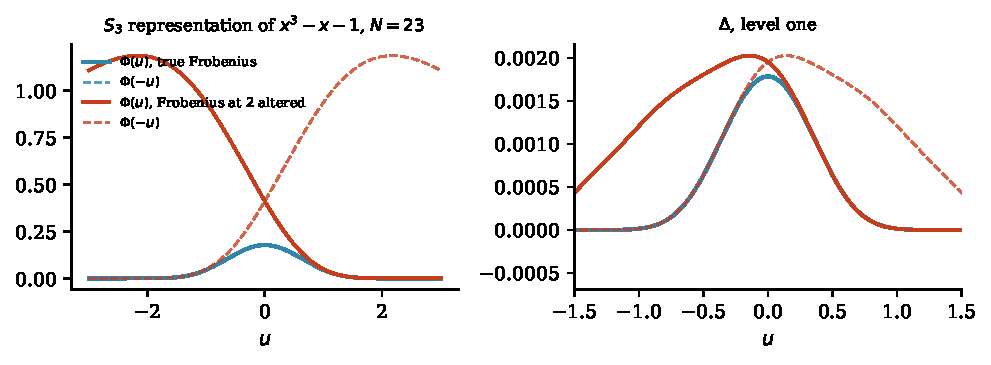
\includegraphics[width=\textwidth]{figs/recip_kernel.pdf}
\caption{Reciprocity as a symmetry. The P\'olya kernel $\Phi_f(u)$ built from Frobenius traces (blue) coincides with $\Phi_f(-u)$ (dashed). Changing the Frobenius data at the single prime $2$ (red) destroys the symmetry. Left: the $S_3$ representation of conductor $23$; right: $\Delta$.}\label{fig:recipkernel}
\end{figure}

\section{The Galois side: Rankin Selberg subordinators}\label{sec:recipgalois}

Infinite divisibility on the Galois side comes for free once one passes to $\rho\otimes\check\rho$. Let $S$ be the set of ramified primes and
\begin{gather*}
D^S(s)=L^S(s,\rho\otimes\check\rho)=\prod_{p\notin S}\det\bigl(1-(\rho\otimes\check\rho)(\Frob_p)p^{-s}\bigr)^{-1},\\
\log D^S(s)=\sum_{p\notin S}\sum_{m\ge1}\frac{|a_\rho(p^m)|^2}{m\,p^{ms}} .
\end{gather*}
All logarithmic coefficients are nonnegative, so for $\sigma>1$ the function $\lambda\mapsto D^S(\sigma+\lambda)/D^S(\sigma)$ is the Laplace transform of a compound Poisson subordinator $X_\sigma$ with L\'evy measure $\sum_{p,m}|a_\rho(p^m)|^2m^{-1}p^{-m\sigma}\delta_{m\log p}$. This is the Galois counterpart of the Rankin Selberg laws of Theorem~\ref{thm:ch09rs} and of the zeta subordinators of Chapter~\ref{ch:10d}.

\begin{theorem}[Gamma shape detects irreducibility; this book]\label{thm:recipgamma}
Let $\rho$ be an Artin representation and $m=\langle\rho,\rho\rangle$ the sum of the squares of the multiplicities of its irreducible constituents. As $\sigma\downarrow1$, $(\sigma-1)X_\sigma$ converges in law to the Gamma law with shape $m$ and scale $1$. In particular $\rho$ is irreducible if and only if the limit is the standard exponential law.
\end{theorem}

\begin{proof}
By Schur's lemma the trivial representation occurs in $\rho\otimes\check\rho=\operatorname{End}(\rho)$ with multiplicity $\langle\rho,\rho\rangle=m$, so by Lemma~\ref{lem:recipvirtual} for $\psi=\rho\otimes\check\rho$ (finitely many Euler factors change nothing near $s=1$), $D^S(s)=(s-1)^{-m}G(s)$ with $G$ holomorphic and nonzero near $1$, and
\[
\E e^{-\lambda(\sigma-1)X_\sigma}=\frac{D^S(\sigma+\lambda(\sigma-1))}{D^S(\sigma)}=\frac{G(\sigma+\lambda(\sigma-1))}{(1+\lambda)^{m}G(\sigma)}\to(1+\lambda)^{-m}
\]
for every $\lambda\ge0$. The continuity theorem for Laplace transforms finishes the proof.
\end{proof}

The Gamma law with shape $m$ is a generalized gamma convolution with Thorin measure $m\,\delta_1$, so the multiplicity $\langle\rho,\rho\rangle$ appears as a Thorin atom of mass $m$, much as the order of central vanishing appears in Chapter~\ref{ch:10b} as a degenerate Thorin atom at the origin. On the automorphic side the Rankin Selberg theory of Jacquet, Shalika, Moeglin and Waldspurger \cite{jacquetshalika1981,moeglinwaldspurger1989} gives the same limit with $m=1$ precisely for cuspidal $\pi$, so ``irreducible Artin representation corresponds to cuspidal automorphic representation'' has a probabilistic shadow: \emph{both are the exponential law}. Figure~\ref{fig:recipgamma} shows the convergence for the $S_3$ representation ($m=1$) and for $\rho\oplus\rho$ ($m=4$), computed from the complete product $L(s,\rho\otimes\rho)=\zeta(s)L(s,\chi_{-23})L(s,\rho)$, which keeps the Euler factor $(1-23^{-s})^{-2}$ that $D^S$ omits and has the same limit. At $\sigma=1.001$ the Laplace transforms at $\lambda=1$ are $0.50059$ and $0.06279$, against $\frac12$ and $\frac1{16}$.

\begin{figure}[t]
\centering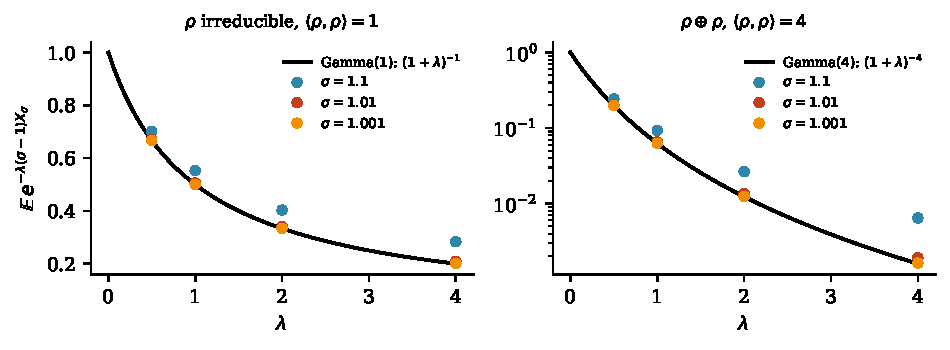
\includegraphics[width=\textwidth]{figs/recip_gamma.pdf}
\caption{Theorem~\ref{thm:recipgamma}: Laplace transforms of $(\sigma-1)X_\sigma$, computed from the complete product $L(s,\rho\otimes\rho)$, for the $S_3$ representation and for $\rho\oplus\rho$, against the Gamma laws with shapes $1$ and $4$.}\label{fig:recipgamma}
\end{figure}

\section{The swap: primes to zeros, computed from Frobenius}\label{sec:recipswap}

The heat trace $\mathcal W_\pi=k_\pi$ of Chapter~\ref{ch:10d}, a sum of $e^{-x\gamma^2}$ over the pairs of zeros $\frac12\pm i\gamma$ (over $\gamma>0$ under GRH), is a function of the zeros, and for automorphic $\pi$ the explicit formula \eqref{eq:10dweil} expresses it through the primes, as Table~\ref{tab:10dheat} does for $\Delta$. The key point for reciprocity is that the prime expression makes sense for any Galois representation, automorphic or not.

\begin{definition}\label{def:recipheat}
Let $\rho$ be self dual, $\Lambda_\rho(n)$ the coefficients of $-L'/L(s,\rho)$ (so $\Lambda_\rho(p^m)=a_\rho(p^m)\log p$ at unramified $p$), and $\gamma(s,\rho)$, $N_\rho$ its gamma factor and conductor. For $x>0$ the \emph{Galois heat trace}\index{heat trace} is
\[
\begin{split}
\mathcal W_\rho(x)={}&\frac1{4\pi}\int_{\R}e^{-xt^2}\Bigl(\log N_\rho+2\operatorname{Re}\frac{\gamma'}{\gamma}\bigl(\tfrac12+it,\rho\bigr)\Bigr)dt\\
&-\frac1{2\pi}\sum_{n\ge2}\frac{\Lambda_\rho(n)}{\sqrt n}\sqrt{\frac\pi x}\,e^{-(\log n)^2/(4x)}.
\end{split}
\]
\end{definition}

The series converges absolutely for every $x>0$, since $|\Lambda_\rho(n)|\le\dim\rho\cdot\log n$ for an Artin representation (more generally $|\Lambda_\rho(n)|\le\dim\rho\cdot n^{\theta}\log n$ when the Satake parameters at every $p$ are bounded by $p^{\theta}$) and the Gaussian factor decays faster than any power of $n$. So $\mathcal W_\rho$ is defined from Frobenius traces, the conductor and the gamma factor alone, with no analytic continuation. To accuracy about $e^{-A}$ only the prime powers with $\log n\le x+\sqrt{x^2+4xA}$, about $\sqrt{4xA}$ for small $x$, matter, so small $x$ needs few primes.

\begin{theorem}[Holomorphy and GRH from the Galois heat trace; this book, after Weil \cite{weil1952,weil1972}]\label{thm:recipcm}
Let $\rho$ be self dual, and suppose $\Lambda(s,\rho)$ has meromorphic continuation of finite order with $\Lambda(s,\rho)=\pm\Lambda(1-s,\rho)$. Write its zeros and poles as $\frac12\pm i\gamma$. Then:
\begin{enumerate}
\item[(i)] $\mathcal W_\rho(x)=\frac12\sum_{\text{zeros}}e^{-x\gamma^2}-\frac12\sum_{\text{poles}}e^{-x\gamma^2}$, with multiplicity, the sums absolutely convergent for $x>0$.
\item[(ii)] $\mathcal W_\rho$ is completely monotone on $(0,\infty)$ if and only if $\Lambda(s,\rho)$ is entire and all its zeros lie on $\operatorname{Re}s=\frac12$.
\end{enumerate}
In particular, for an Artin representation with real character and no trivial constituent (a trivial constituent of multiplicity $r$ adds the pole term $-re^{x/4}$), Artin's conjecture together with GRH for $L(s,\rho)$ is equivalent to the complete monotonicity of a function computed from Frobenius traces.
\end{theorem}

\begin{proof}
(i) is Weil's explicit formula \cite{weil1952} (see \cite{iwanieckowalski2004}, Theorem~5.12) for the even test function $h(t)=e^{-xt^2}$, whose Fourier transform is $\sqrt{\pi/x}\,e^{-u^2/(4x)}$; $h$ is entire and decays in every horizontal strip, so the contour shifts are justified, and poles enter with the opposite sign to zeros. Self duality makes the prime side real and equal to $-\frac1\pi\sum\Lambda_\rho(n)n^{-1/2}\hat h(\log n)$.

(ii) If $\Lambda$ is entire with all $\gamma$ real, (i) exhibits $\mathcal W_\rho$ as the Laplace transform of the positive measure $\frac12\sum\delta_{\gamma^2}$, as in Theorem~\ref{thm:10bmain}(d), which is the automorphic case. Conversely let $\mathcal W_\rho$ be completely monotone, so $\mathcal W_\rho(x)=\int_{[0,\infty)}e^{-xu}\mu(du)$ with $\mu\ge0$ by Bernstein's theorem. Write (i) as $\sum_kc_ke^{-xw_k}$ with distinct $w_k=\gamma_k^2\in\C$ and nonzero weights $c_k$, half the multiplicity, negative for poles. A pole and a zero cannot share a value of $w$: by the functional equation the zero and pole sets are each symmetric under $\gamma\mapsto-\gamma$, and $\gamma^2$ determines $\gamma$ up to sign. All zeros and poles lie in $0\le\operatorname{Re}s\le1$, by the Euler product and the functional equation, so $|\operatorname{Im}\gamma_k|\le\frac12$ and $\operatorname{Re}w_k\ge-\frac14$. Since $\Lambda$ has finite order, the numbers of zeros and poles with $|\gamma|\le T$ grow at most polynomially in $T$, so $\sum_k|c_k|e^{-x\operatorname{Re}w_k}\ll x^{-A}$ as $x\to0$ for some $A$. Fix an integer $M>A+1$. The transform
\[
J(s)=\int_0^\infty e^{-sx}x^M\mathcal W_\rho(x)\,dx
\]
converges for $\operatorname{Re}s$ large, and integrating term by term in each representation,
\[
J(s)=\sum_k\frac{M!\,c_k}{(s+w_k)^{M+1}}=\int_{[0,\infty)}\frac{M!\,\mu(du)}{(s+u)^{M+1}}.
\]
The series converges absolutely and locally uniformly off the points $-w_k$, because $|w_k|\asymp|\gamma_k|^2$ and the counting function grows polynomially, so it defines a meromorphic function on $\C$ with a pole of order $M+1$ at each $-w_k$. The integral is holomorphic on $\C\setminus(-\infty,0]$. Since the two agree for $\operatorname{Re}s$ large, they agree everywhere, so every $-w_k$ lies in $(-\infty,0]$: every $w_k$ is real and nonnegative. With real exponents, uniqueness of the Laplace transform of measures on $[0,\infty)$ gives $\mu=\sum c_k\delta_{w_k}$, so every $c_k$ is positive. Hence there are no poles, so $\Lambda$ is entire, and every $\gamma_k$ is real, since $\gamma_k^2=w_k\ge0$.
\end{proof}

Complete monotonicity is a positivity condition on infinitely many derivatives, but each instance $(-1)^j\mathcal W_\rho^{(j)}(x)\ge0$ is a finite computation with Frobenius traces. A pair of poles of $\Lambda$ at $\frac12\pm iT$ contributes $-e^{-xT^2}$, but it is invisible near $x=T^{-2}$: there the prime sum is of order $Te^{-(T\log2)^2/4}$, so $\mathcal W_\rho(T^{-2})$ is fixed by the conductor and the gamma factor, and as soon as there are ordinates in $(\frac12T,T)$ and in $(T,\frac32T)$ they outweigh the pole term in every inequality $(-1)^j\mathcal W_\rho^{(j)}(T^{-2})\ge0$. A pole midway between consecutive ordinates $2\delta$ apart first violates an inequality near $x=j/T^2$ with $j\approx\frac{\log2}2(T/\delta)^2$ (Exercise~\ref{ex:recippole}). So the inequalities can disprove Artin's conjecture or GRH for $\rho$, one violation at a time, but no finite set of them is known to verify either to any finite height. Booker's verification of Artin's conjecture to finite height \cite{booker2006} combines a group theoretic criterion with the location of zeros by the explicit formula and Turing's method.

The swap is also rigid.

\begin{proposition}[The swap sees every prime; this book]\label{prop:reciprigid}
Let $\rho$ satisfy the conclusion of Theorem~\ref{thm:recipcm}(ii), and let $\rho'$ be self dual Galois data with the same conductor and the same gamma factor, whose local factors differ from those of $\rho$ at a nonempty set $P$ of primes with $\sum_{p\in P}p^{-1/2}\log p<\infty$; suppose that the Satake parameters of $\rho$ and $\rho'$ have absolute value at most $1$. Then $\mathcal W_{\rho'}$ is not completely monotone. In particular, if $\Lambda(s,\rho')$ has meromorphic continuation of finite order with $\Lambda(s,\rho')=\pm\Lambda(1-s,\rho')$, it has a pole or a zero off the critical line.
\end{proposition}

\begin{proof}
By the cosine form \eqref{eq:recipcospair} of the Laplace pair \eqref{eq:10dpair},
\[
\mathcal W_{\rho'}(x)-\mathcal W_\rho(x)=\int_0^\infty e^{-xz}g(z)\,dz,
\]
where $c_{p,m}=\Lambda_{\rho'}(p^m)-\Lambda_\rho(p^m)$ and
\[
g(z)=-\frac1{2\pi\sqrt z}\sum_{p\in P}\sum_{m\ge1}\frac{c_{p,m}}{p^{m/2}}\cos(\sqrt z\,m\log p).
\]
By hypothesis the coefficients are absolutely summable, so $\sqrt z\,g(z)$ is a nonzero uniformly almost periodic function of $r=\sqrt z$ with distinct frequencies $m\log p$ (unique factorisation) and no constant term. If $\mathcal W_{\rho'}$ were completely monotone it would be the Laplace transform of $\mu'\ge0$, and by uniqueness $\mu'=\frac12\sum\delta_{\gamma^2}+g(z)dz$. The absolutely continuous part of a positive measure is nonnegative, so $g\ge0$ almost everywhere. But a nonzero almost periodic function with mean zero takes negative values on a set of positive measure.
\end{proof}

Compare Proposition~\ref{prop:01limits}: altering Frobenius data on a set of primes of density zero changes no distributional statement, but by Proposition~\ref{prop:reciprigid} it destroys the Galois heat trace whenever $\sum_{p\in P}p^{-1/2}\log p<\infty$; a single prime suffices.

Figure~\ref{fig:recipheat} tests this on the $S_3$ representation of conductor $23$, which is automorphic (it is the weight one form $\eta(z)\eta(23z)$; its first zero, $\gamma_1=5.1157$, and its Thorin data are in Table~\ref{tab:10bcatalogue}). The Galois heat trace was computed from Frobenius classes obtained by factoring $x^3-x-1$ modulo primes below $60000$, with no use of the modular form. It agrees with the sum over the zeros of $L(s,\rho)$ to all $16$ digits at $x=0.02$ (both give $1.4102560772724$), to an absolute error of $1.5\cdot10^{-16}$ at $x=0.3$ and to $10^{-8}$ relative at $x=0.7$, where double precision runs out. With the class of $\Frob_2$ changed from order three to the identity, the same function becomes negative from $x=0.1$ on ($-0.32$ at $x=0.1$, $-0.62$ at $x=0.5$), so it is not even positive, let alone completely monotone.

\begin{figure}[t]
\centering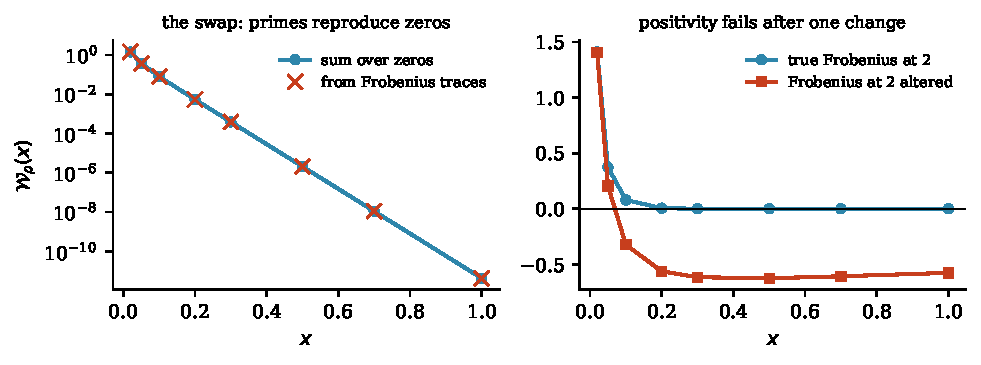
\includegraphics[width=\textwidth]{figs/recip_heat.pdf}
\caption{Left: the Galois heat trace of Definition~\ref{def:recipheat} for the $S_3$ representation, computed from Frobenius classes alone (crosses), against the sum over zeros (line). Right: changing the Frobenius class at $2$ makes it negative.}\label{fig:recipheat}
\end{figure}

\section{Van Dantzig duality and the Euler half line}\label{sec:recipvdp}

For a self dual $\Lambda$ with centre $\frac12$, $\Lambda(\frac12)\ne0$ and a nonnegative P\'olya kernel, the van Dantzig pair of Theorem~\ref{thm:10dvdp}, which exists exactly under GRH, is
\[
f_\Lambda(t)=\frac{\Lambda(\frac12+it)}{\Lambda(\frac12)},\qquad g_\Lambda(t)=\frac{\Lambda(\frac12)}{\Lambda(\frac12+t)} .
\]
The first member lives on the critical line, where by \eqref{eq:recipmellin} it is the Fourier transform of the P\'olya kernel, that is of the automorphic form on $i\R_{>0}$. The second lives on the real axis, and for $t>\frac12$ it is the reciprocal of an Euler product times the central value $\Lambda(\frac12)$, that is Galois data up to one constant. The van Dantzig involution $F\mapsto1/F(i\,\cdot)$ passes between the two faces, and the Wald couple $(W,H)$ of Theorem~\ref{thm:10dvdp}(c), with $\E e^{sW}=\Lambda(\frac12+s)/\Lambda(\frac12)$ and $\E e^{-s^2H}=\Lambda(\frac12)/\Lambda(\frac12+s)$, pairs a variable whose density is the automorphic form with a generalized gamma convolution whose transform is the Euler product. This suggests reading reciprocity as the existence of a Wald couple whose two members are built on different sides; the next theorem makes one direction precise, using only the Euler half line.

\begin{theorem}[Euler half line criterion; this book]\label{thm:recipeuler}
Let $\rho$ be self dual with completion $\Lambda(s,\rho)$, defined for $\operatorname{Re}s>1$ by its Euler product, and let $s_0>\frac14$. Suppose that for $s>\frac14$,
\[
\frac{\Lambda(\frac12+\sqrt{s_0},\rho)}{\Lambda(\frac12+\sqrt s,\rho)}=C\,\E e^{-sH}
\]
for a constant $C>0$ and a generalized gamma convolution $H$ whose Thorin measure is $\sum_kc_k\delta_{u_k}$ with positive integers $c_k$ and $u_k>0$. Then $\Lambda(s,\rho)$ extends to an entire function of finite order, $\Lambda(s,\rho)=\Lambda(1-s,\rho)$, every zero lies on $\operatorname{Re}s=\frac12$, and $\Lambda$ is bounded in vertical strips. Conversely, if $\Lambda(s,\rho)$ is entire of order one with this functional equation, $\Lambda(\frac12,\rho)\ne0$ and all zeros on the critical line, then the hypothesis holds with $u_k=\gamma_k^2$.
\end{theorem}

\begin{proof}
A GGC with drift $a\ge0$ and Thorin measure $\sum c_k\delta_{u_k}$ has $\E e^{-sH}=e^{-as}\prod_k(1+s/u_k)^{-c_k}$, with $\sum_kc_k/u_k<\infty$. Since the $c_k$ are positive integers, $E(z)=e^{az^2}\prod_k(1+z^2/u_k)^{c_k}$ is an even entire function of $z$ of finite order. For real $z>\frac12$ we have $\Lambda(\frac12+z,\rho)=C^{-1}\Lambda(\frac12+\sqrt{s_0},\rho)E(z)$, and both sides are holomorphic on $\operatorname{Re}z>\frac12$, so they agree there; the right side provides the continuation of $\Lambda(\frac12+z,\rho)$ to an entire function. Evenness of $E$ is the functional equation, and the zeros of $E$ are at $z=\pm i\sqrt{u_k}$, that is $s=\frac12\pm i\sqrt{u_k}$. On $\operatorname{Re}s=1+\delta$ the completion is bounded because the gamma factor decays and the Euler product is bounded; by the functional equation the same holds on $\operatorname{Re}s=-\delta$; finite order and the Phragm\'en Lindel\"of principle give boundedness in the strip between. The converse is Theorem~\ref{thm:10dduality} applied to $\Lambda(\frac12+z,\rho)$, normalised at $z=\sqrt{s_0}$ instead of $0$.
\end{proof}

Combining Theorem~\ref{thm:recipeuler} with Proposition~\ref{prop:recipsym}, we obtain a Thorin form of Hecke's converse theorem.

\begin{corollary}[Thorin converse theorem at level one; this book]\label{cor:recipconverse}
Let $k\equiv0\bmod4$ and let $(a_p)$ be the Frobenius traces of a self dual Galois representation of conductor $1$ with the gamma factor $\Gamma_{\C}(s+\frac{k-1}2)$, where $\Gamma_\C(s)=\Gamma_\R(s)\Gamma_\R(s+1)=2(2\pi)^{-s}\Gamma(s)$, and Ramanujan bound, with $a_n$ its Dirichlet coefficients. If the normalised Euler product $\Lambda(\frac12+\sqrt{s_0})/\Lambda(\frac12+\sqrt s)$, $s>\frac14$, is a constant times the Laplace transform of a GGC whose Thorin measure is a sum of point masses with positive integer weights, then $\sum a_nn^{(k-1)/2}e^{2\pi inz}$ is a cusp form of weight $k$ for $\SL_2(\Z)$, and it satisfies GRH.
\end{corollary}

\begin{proof}
By Theorem~\ref{thm:recipeuler} the completion is entire, bounded in vertical strips and even about the centre. In the classical normalisation (centre $\frac k2$) this is $\Lambda(k-s)=\Lambda(s)=(-1)^{k/2}\Lambda(s)$, which is (iii) of Proposition~\ref{prop:recipsym} with $N=1$, so $f$ is a cusp form.
\end{proof}

The hypothesis of Corollary~\ref{cor:recipconverse} is stated entirely on the Euler half line, so it is a statement about Galois data; it is stronger than reciprocity, since it includes GRH. Its natural weakening, with nonzero integer weights and complex atoms, always holds for the Artin representations of Open Problem~\ref{op:recipsigned}, where Artin's conjecture is the positivity of the weights.

\subsection{An unconditional Galois family}

Positivity is available unconditionally on the Galois side whenever the logarithmic coefficients are nonnegative, as for Dedekind zeta functions; the case used here is the Rankin Selberg square. For $\alpha>1$ let $F(s)=\Lambda^S(s,\rho\otimes\check\rho)$, the completion of $D^S$ of Section~\ref{sec:recipgalois}.

\begin{proposition}[this book]\label{prop:recipfamily}
For every Artin representation $\rho$ and every $\alpha>1$ there is a GGC $H_\alpha$ with
\[
\frac{F(\alpha)}{F(\alpha+\sqrt s)}=e^{-b_\alpha\sqrt s}\,\E e^{-sH_\alpha},\qquad b_\alpha=\frac{F'(\alpha)}{F(\alpha)},
\]
whose Thorin density is the $2\sin^2$ transport (Lemma~\ref{lem:10dsin2}) of the measure
\[
\sum_{p\notin S,\,m\ge1}|a_\rho(p^m)|^2(\log p)\,p^{-m\alpha}\delta_{m\log p}
\]
($x$ times the L\'evy measure of $X_\alpha$) together with the gamma factor contribution. It is computed from Frobenius traces alone.
\end{proposition}

\begin{proof}
The function $F$ is holomorphic and zero free on $\operatorname{Re}s>1$. The second derivative of $\log F$ along the real axis is the sum of the trigamma terms of the gamma factor and of $\sum|a_\rho(p^m)|^2(m\log p)^2m^{-1}p^{-ms}$, both completely monotone and tending to zero. Lemma~\ref{lem:10dsin2} applies.
\end{proof}

As $\alpha$ decreases to $1$ the pole of order $\langle\rho,\rho\rangle$ appears (Theorem~\ref{thm:recipgamma}). Below $1$ the Euler product no longer defines $F$. Meromorphic continuation of $L(s,\rho\otimes\check\rho)$ is known for every Artin $\rho$ by Brauer's theorem, and holomorphy away from $s=1$ follows from automorphy of $\rho$ by the Rankin Selberg theory; neither gives positivity. For automorphic $\rho$, apply the argument of Theorem~\ref{thm:10dshift} to the complete function $\Lambda(s,\rho\otimes\check\rho)$, all Euler factors included and the poles at $s=0,1$ removed: its transforms at the base points $\alpha\in(\frac12,1]$ are GGCs, with nonnegative Thorin densities $V_{\alpha-1/2}$, for every such $\alpha$ exactly when GRH holds for $L(s,\rho\otimes\check\rho)$, and the densities then converge to the Thorin measure of the zeros as $\alpha\downarrow\frac12$. For irreducible two dimensional $\rho$ this GRH contains the Riemann hypothesis, since $L(s,\rho\otimes\check\rho)=\zeta(s)L(s,\operatorname{Ad}\rho)$ with $L(s,\operatorname{Ad}\rho)$ entire \cite{gelbartjacquet1978}. Splitting off the factor $e^{-b_\alpha\sqrt s}$ as in Proposition~\ref{prop:recipfamily}, with $b_\alpha$ now the logarithmic derivative of this complete function at $\alpha$, leaves the densities $V_{\alpha-1/2}-b_\alpha/(2\pi\sqrt z)$ (Lemma~\ref{lem:10dsin2}), and their positivity below $\alpha=1$ is not known to follow from GRH; for $\xi$ it follows from the Riemann hypothesis by a theorem of Lagarias, and is not known unconditionally (Section~\ref{sec:10daway}). \emph{Continuing a family of positive measures, defined from Frobenius traces above the line $\operatorname{Re}s=1$, down to the centre while preserving positivity} is the probabilistic form of the problem that this chapter proposes; for the Rankin Selberg square it is holomorphy away from $s=1$ together with GRH for $L(s,\rho\otimes\check\rho)$, which does not by itself give reciprocity.

\section{The programme}\label{sec:recipprogramme}

The equivalences of this chapter prove nothing new about reciprocity; like the Thorin forms of the Riemann hypothesis, they move the difficulty rather than remove it. They offer positivity and symmetry statements about Galois data, to which probabilistic tools apply and which can be tested one prime at a time.
\begin{enumerate}
\item Symmetry. At level one, reciprocity is the evenness (oddness when $k\equiv2\bmod4$) of the P\'olya kernel built from Frobenius traces (Proposition~\ref{prop:recipsym}). At level $N$ it is the pairing of twisted kernels required by Weil's converse theorem.
\item Positivity. For self dual $\rho$ with meromorphic continuation of finite order and a functional equation, holomorphy together with GRH is the complete monotonicity of the Galois heat trace (Theorem~\ref{thm:recipcm}), a function of Frobenius traces each of whose derivatives is computable at each $x$ to any accuracy in finitely many steps. One certified violation disproves holomorphy or GRH; no finite set of verified inequalities is known to prove them to any finite height.
\item Rigidity. The Galois heat trace detects a change of Frobenius data at a single prime (Proposition~\ref{prop:reciprigid}), in contrast with every distributional statement (Proposition~\ref{prop:01limits}).
\item Continuation. On the Euler half line the Galois side produces GGCs, from the Rankin Selberg square unconditionally (Proposition~\ref{prop:recipfamily}) and from $\rho$ itself under the Thorin hypothesis (Theorem~\ref{thm:recipeuler}). Holomorphy together with GRH, for $L(s,\rho\otimes\check\rho)$ in the first case and for $L(s,\rho)$ in the second, is the continuation to the centre of the corresponding GGCs (for the Rankin Selberg square with its poles removed and the drift kept inside, as in Theorem~\ref{thm:10dshift}); at level one the second gives reciprocity (Corollary~\ref{cor:recipconverse}).
\item Laws. On the Frobenius probability space reciprocity is almost sure equality, and its uniqueness statements, the correspondence of irreducible with cuspidal and, for every $\epsilon>0$, agreement within $\epsilon$ outside a set of primes of Dirichlet density zero follow from two orthonormality theorems (Corollary~\ref{cor:reciplaw}); class field theory is measurability with respect to congruences (Proposition~\ref{prop:recipcongruence}). Laws cannot give existence; the objects of items 1 to 3 see individual primes, but they too give existence only through a converse theorem.
\item Gamma processes. Equidistribution of Frobenius data is a Gamma process limit of the labelled factorisation of a random integer (Theorem~\ref{thm:recipgammaproc}); reciprocity laws are vanishing statements for Thorin measures (Theorem~\ref{thm:recipthorin}); and comparing an Artin representation with a cuspidal one gives a conjectured zero two law (Conjecture~\ref{conj:recipmixed}), the orthogonality half of reciprocity: it is implied by reciprocity and asserts no existence, and the existence of a partner is the other half.
\item Gaussian model. For $\GL_1$ the symmetry part of the programme runs, and the circle models the positivity part: the theta transformation, proved from the normal characteristic function or by Fej\'er positivity of the winding number terms, gives quadratic reciprocity and Gauss's sign (Section~\ref{sec:recipgauss}).
\item Irreducibility. The Gamma shape of the Rankin Selberg subordinator is $\langle\rho,\rho\rangle$ (Theorem~\ref{thm:recipgamma}), the probabilistic shadow of ``irreducible corresponds to cuspidal''.
\end{enumerate}

The most concrete target is the even icosahedral case, where reciprocity is open and the Galois data are explicit. For such $\rho$ every quantity above can be computed from the Frobenius classes. Factorisation patterns modulo $p$ give these only up to Galois conjugacy, so they cannot tell apart the two classes of elements of order $5$ in the projective image $A_5$, on whose preimages the traces of $\rho$ differ; a Frobenius resolvent separates them \cite{dokchitser2013}. When $\det\rho$ is trivial, so that $\rho$ is self dual, item~2 tests Artin's conjecture together with GRH (Problem~\ref{cp:recipicosa}). The analogue of Proposition~\ref{prop:recipsym} for the gamma factor $\Gamma_\R(s)^2$ or $\Gamma_\R(s+1)^2$ of an even representation (as complex conjugation acts by $1$ or $-1$), with a $K$ Bessel kernel in place of the exponential, gives symmetry tests for the twisted kernels.

\subsection{Open problems}

\begin{problem}[The Thorin converse theorem in general]\label{op:recipgln}
Formulate and prove a version of Theorem~\ref{thm:recipeuler} for twists $\rho\times\pi'$ that are not self dual, strong enough to combine with the converse theorem of Cogdell and Piatetski Shapiro. The obstacle is that the completion $\Xi_\rho$ of Definition~\ref{def:10bxi}, built from $\Lambda(\frac12+z,\rho)\Lambda(\frac12+z,\check\rho)$, controls the product of two $L$ functions, whereas converse theorems need each one.
\end{problem}

\begin{problem}[Descending the base point]\label{op:recipdescent}
For automorphic $\rho$, positivity of the densities $V_{\alpha-1/2}$, with the drift kept inside, for every $\alpha\in(\frac12,1]$ is GRH for $L(s,\rho\otimes\check\rho)$ (end of Section~\ref{sec:recipvdp}). Decide whether the densities $V_{\alpha-1/2}-b_\alpha/(2\pi\sqrt z)$ of that section, with the drift split off, also stay nonnegative there, which for $\xi$ holds under the Riemann hypothesis and is proved unconditionally for $\alpha\ge1$ (Section~\ref{sec:10daway}) and for $\frac12<\alpha<1$ below height $3\times10^{12}$ (Chapter~\ref{ch:beta}), and identify the obstruction to positivity below $\alpha=1$ in terms of Frobenius data alone: which features of the L\'evy measure of $X_\alpha$ at $\alpha>1$ control the sign of the transported density at $\alpha<1$? For $\xi$ and $\Delta$ the computational counterpart is the problem on transported Thorin densities in the strip in Chapter~\ref{ch:10d}.
\end{problem}

\begin{problem}[Signed Thorin measures]\label{op:recipsigned}
For an Artin representation $\rho$ with real character, no trivial constituent, root number $1$ and $\Lambda(\frac12,\rho)$ finite and nonzero, Brauer's theorem and Hadamard factorisation give, for a fixed $s_0>\frac14$, $\Lambda(\frac12+\sqrt{s_0},\rho)/\Lambda(\frac12+\sqrt s,\rho)=C\prod_k(1+s/u_k)^{-c_k}$ with nonzero integers $c_k$ and complex $u_k=\gamma_k^2$, where $c_k<0$ exactly at poles, and $u_k\notin(0,\infty)$ exactly at zeros and poles off the critical line. Artin's conjecture for $\rho$ is the statement that every $c_k$ is positive. Find a property of the signed L\'evy measure of $\log\Lambda(s,\rho)$ on the Euler half line, that is of Frobenius data, which forces every $c_k$ to be positive without forcing the $u_k$ to be real, so that holomorphy is separated from GRH (compare Section~\ref{sec:10bparabola}).
\end{problem}

\begin{problem}[A Fej\'er summation for primes]\label{op:recipfejer}
Find positive weights $w_N(n)\le1$ with $w_N(n)\to1$ such that the prime side of Definition~\ref{def:recipheat}, with $\Lambda_\rho(n)$ replaced by $w_N(n)\Lambda_\rho(n)$ and the archimedean term adjusted accordingly, is the Laplace transform of a positive measure, and such that positivity for each $N$ follows from Frobenius data alone, as Fej\'er positivity does for the circle (Proposition~\ref{prop:recipfejer}); otherwise $w_N\equiv1$ works whenever holomorphy and GRH hold. By Theorem~\ref{thm:recipcm} this would prove holomorphy and GRH for $L(s,\rho)$; the problem is to see what positivity of this kind forces on Frobenius data (compare Open Problem~\ref{op:thorin}).
\end{problem}

\begin{problem}[Reciprocity in law versus reciprocity]\label{op:reciplaw}
Show that if an irreducible Artin representation $\rho$ is reciprocal in law with a cuspidal $\pi$ (Corollary~\ref{cor:reciplaw}), then $a_\rho(p)=a_\pi(p)$ for all but finitely many $p$ (compare Open Problem~\ref{op:inverse} and Corollary~\ref{cor:01functional}). It holds whenever $\rho$ is known to be automorphic, by Corollary~\ref{cor:reciplaw}(v); for $n=2$, where this leaves the even icosahedral $\rho$, it would follow from a refinement of Ramakrishnan's theorem \cite{ramakrishnan1994} to the case in which one member is Galois and the agreement is only approximate, as in Corollary~\ref{cor:reciplaw}(iv); in general it is a strong multiplicity one statement across the two sides.
\end{problem}

\begin{problem}[The mixed zero two law]\label{op:recipmixed}
Show that meromorphy of $L(s,\rho\times\tilde\pi)$ near $\operatorname{Re}s=1$, with at most a simple pole at $s=1$ and no zeros on the line, gives the dichotomy of Conjecture~\ref{conj:recipmixed} by the argument of Theorem~\ref{thm:recipzerotwo} and reduces the rest of the conjecture to a form of Open Problem~\ref{op:reciplaw}, and prove the conjecture for one even icosahedral Artin representation.
\end{problem}

\begin{problem}[Joint marked processes]\label{op:recipjoint}
Show that the joint limit of the marked processes of Theorem~\ref{thm:recipgammaproc} exists for an Artin representation $\rho$ and a cuspidal $\pi$ of the same dimension; it is not determined by the two marginal limits (compare Exercise~\ref{ex:recipjoint} and Theorem~\ref{thm:04joint}). Is the joint label law either supported on $\{a_\rho=a_\pi\}$, or such that the Thorin measure of $|a_\rho-a_\pi|^2$ has mass bounded below by a constant depending only on $n$?
\end{problem}

\begin{problem}[Signs of drifts]\label{op:recipdrift}
When does the split class approach its Gamma limit from above, $\kappa_{\{1\}}<0$ in Theorem~\ref{thm:recipdrift}? This requires $\gamma_K^S<0$. Characterise such fields and relate the signs of the $\kappa_C$ to the bias between classes that Section~\ref{sec:ch3cheb} measures for the field of Example~\ref{ex:ch3cubic} (Exercise~\ref{ex:ch3fs}), and to the Chebotarev races of the computational problems of Chapter~\ref{ch:03}.
\end{problem}

\section{Notes}

Reciprocity in the form used here is from Langlands' letter and lectures \cite{langlands1967,langlands1970}; the known cases cited are \cite{langlands1980,tunnell1981,wiles1995,taylorwiles1995,bcdt2001,kharewintenberger2009,kharewintenberger2009b,kisin2009}; potential automorphy is from \cite{hsbt2010,blght2011} and symmetric power functoriality from \cite{newtonthorne2021,newtonthorne2021b}. Artin's conjecture and Brauer's theorem are \cite{artin1924,brauer1947}, and Artin's reciprocity law is \cite{artin1927}. Converse theorems are due to Hecke \cite{hecke1936}, Weil \cite{weil1967}, Jacquet and Langlands \cite{jacquetlanglands1970} and Cogdell and Piatetski Shapiro \cite{cogdellps1994}. The Rankin Selberg pole is from Jacquet and Shalika \cite{jacquetshalika1981} and Moeglin and Waldspurger \cite{moeglinwaldspurger1989}. Theorem~\ref{thm:recipcm}(ii) is Weil's positivity criterion \cite{weil1952,weil1972} restricted to the test functions $t^{2j}e^{-xt^2}$; Weil's extension of the explicit formula to Artin Hecke $L$ functions \cite{weil1972} already ties positivity to Artin's conjecture together with GRH. The Thorin framework for automorphic $L$ functions of Chapters~\ref{ch:10b} to \ref{ch:10d} extends the first author's work \cite{polson2017,polson2018vdp}; the sine squared lemma is Lemma~14 of \cite{polson2018vdp}, with its first step from Roynette and Yor \cite{roynetteyor2005}, who also introduced Wald couples with infinitely divisible members; van Dantzig pairs and Wald couples for $\xi$ are in \cite{roynetteyor2005,polson2018vdp,konstantopoulospatiesarkar2024}. The theta transformation goes back to Jacobi and Poisson; reciprocity for Gauss sums is due to Schaar \cite{schaar1850} and Landsberg \cite{landsberg1893}, and the derivation of quadratic reciprocity from it is in Dym and McKean \cite{dymmckean1972}. Our proofs in Section~\ref{sec:recipgauss} differ only in reading Poisson summation as the Fourier series of a wrapped normal law and Fej\'er's proof of it as a Laplace transform through the pair of the $2\sin^2$ lemma (Proposition~\ref{prop:recipfejer}). Zolotarev's proof \cite{zolotarev1872}, through signs of permutations, is another short route to Corollary~\ref{cor:recipqr}. Dedekind sums and their reciprocity law are treated in \cite{rademachergrosswald1972}. Poisson random measures and the Gamma process are in Kingman \cite{kingman1993}, the Dirichlet process in Ferguson \cite{ferguson1973}, and generalized gamma convolutions in Thorin \cite{thorin1977} and Bondesson \cite{bondesson1992}. Sato Tate for newforms and its joint form are \cite{blght2011,harris2009}. Euler Kronecker constants are Ihara's \cite{ihara2006}; negative values for cyclotomic fields are in \cite{fordlucamoree2014}. Ours are Theorems~\ref{thm:recipgammaproc}, \ref{thm:recipggcfun}, \ref{thm:recipthorin}, \ref{thm:recipzerotwo} and \ref{thm:recipdrift} in the forms stated, the bounds (i) and (ii) of Theorem~\ref{thm:recipheat}, Corollary~\ref{cor:recipchebgamma}, Conjecture~\ref{conj:recipmixed} with Proposition~\ref{prop:recipmixed}, the probabilistic formulations of Section~\ref{sec:reciplaw}, Corollary~\ref{cor:reciplaw}, Proposition~\ref{prop:recipcongruence} (a reformulation of Chebotarev's theorem for $K(\zeta_N)$), Proposition~\ref{prop:recipsym} in this form, Theorem~\ref{thm:recipgamma}, Definition~\ref{def:recipheat}, Theorem~\ref{thm:recipcm}, Proposition~\ref{prop:reciprigid}, Theorem~\ref{thm:recipeuler}, Corollary~\ref{cor:recipconverse}, Proposition~\ref{prop:recipfamily} and the computations; each rests on the cited theory.

\section{Exercises}

\begin{enumerate}
\item\label{ex:recipdelta} Show that the kernel $\Phi_f$ of \eqref{eq:recipmellin} for $f=\Delta$ is $\Lambda(6,\Delta)\Phi_\Delta$, with $\Phi_\Delta$ the normalised kernel of Chapters~\ref{ch:02} and \ref{ch:10}, so that its evenness, proved there, is the case $N=1$, $k=12$ of Proposition~\ref{prop:recipsym}. For a newform $f$ of level $N$ and trivial character, and a primitive character $\chi$ modulo $q$ with $(q,N)=1$, write the relation between $\Phi_{f\otimes\chi}(-u)$ and $\Phi_{f\otimes\bar\chi}(u)$ that Weil's converse theorem requires, with its constant.
\item\label{ex:recipshape} For the $S_3$ representation $\rho$ of $x^3-x-1$, show that $\rho\otimes\rho\cong\mathsf{1}\oplus\operatorname{sgn}\oplus\rho$ and $L(s,\rho\otimes\rho)=\zeta(s)L(s,\chi_{-23})L(s,\rho)$, and deduce the shape $1$ in Theorem~\ref{thm:recipgamma}. What is the shape for $\mathsf{1}\oplus\operatorname{sgn}$?
\item\label{ex:recipgauss} Identify, prime by prime, the Laplace transform in Proposition~\ref{prop:reciprigid} with the oscillatory part of a local Thorin comb (Proposition~\ref{prop:10cdictionary}). Compare it with the winding number terms of Proposition~\ref{prop:recipfejer}: why do the cosine densities of all winding numbers, summed with Fej\'er weights, give point masses, while those of the powers of a single prime give a signed density?
\item\label{ex:recippole} Suppose $\Lambda(s,\rho)$ has simple poles at $\frac12\pm iT$, $\Lambda(\frac12,\rho)\ne0$, and is otherwise as in GRH, with positive ordinates $\gamma_1<\gamma_2<\cdots$. Show that $\mathcal W_\rho(x)<0$ for all large $x$ if $T<\gamma_1$. If $\frac12T<\gamma_n<T<\gamma_{n+1}<\frac32T$, show that every inequality $(-1)^j\mathcal W_\rho^{(j)}(T^{-2})\ge0$ holds, but that $(-1)^j\mathcal W_\rho^{(j)}(j/T^2)<0$ for all large $j$; when $T$ is the midpoint and $2\delta=\gamma_{n+1}-\gamma_n$ is small compared with $T$, the least such $j$ is about $\frac{\log2}2(T/\delta)^2$. (For the $S_3$ representation of conductor $23$ and $T$ midway between $\gamma_1$ and $\gamma_2$ the first violation is at $j=13$, near $x=13.5/T^2$.)
\item\label{ex:recipgenls} Apply Lemma~\ref{lem:recipwrap} with $y\ne0$ in the proof of Theorem~\ref{thm:recipls} to obtain reciprocity for $\sum_{n\bmod c}e^{\pi i(an^2+bn)/c}$ when $ac+b$ is even.
\item\label{ex:recipdedekind} Let $K$ be uniform on $\Z/c\Z$, let $((x))=x-\lfloor x\rfloor-\frac12$ for $x\notin\Z$ and $((x))=0$ otherwise, and let $s(b,c)=\sum_{k\bmod c}((k/c))((bk/c))$ be the Dedekind sum. Show that $s(b,c)$ is $c$ times the covariance of $((K/c))$ and $((bK/c))$, and that for $U$ uniform on $[0,1)$ the covariance of $((bU))$ and $((cU))$ is $1/(12bc)$ when $\gcd(b,c)=1$. Explain why this does not yet give Dedekind's reciprocity law $s(b,c)+s(c,b)=\frac{b^2+c^2+1}{12bc}-\frac14$. A probabilistic proof of the reciprocity law, and an extension of Theorem~\ref{thm:recipheat} to the Dedekind eta function, whose multiplier involves Dedekind sums, are left open.
\item\label{ex:recipjoint} For the $S_3$ representations $\rho$ and $\rho_{31}$ of the text, compute the limiting joint law of $(a_\rho,a_{\rho_{31}})$ and check that $d(\rho,\rho_{31})^2=2$. What is the joint law for $\rho$ and $\rho\otimes\chi_{-23}$, and what is $d$?
\item\label{ex:recipwald} Show that for $s>\frac12$ the Wald couple identity $\E e^{sW}\E e^{-s^2H}=1$ involves $\Lambda$ only through the Euler product values $\Lambda(\frac12+s)$ and the single central value $\Lambda(\frac12)$. Show that a random variable $W$ with $\E e^{sW}=\Lambda(\frac12+s)/\Lambda(\frac12)$ for all $s>\frac12$, if it exists, has its law determined by these values (tilt by $e^{s_0W}$ with $s_0>\frac12$), and explain why the identity on $s>\frac12$ cannot by itself show that such a $W$ exists.
\end{enumerate}

\section{Open computational problems}

\begin{compproblem}[Even icosahedral representations]\label{cp:recipicosa}
Objective: for an icosahedral Artin representation $\rho$ with trivial determinant (hence self dual and even) from the LMFDB, compute the Galois heat trace of Definition~\ref{def:recipheat} and its derivatives in ball arithmetic and search for a certified violation of $(-1)^j\mathcal W_\rho^{(j)}(x)\ge0$, which by Theorem~\ref{thm:recipcm} would disprove Artin's conjecture or GRH for $\rho$. Objects and scale: one representation, prime powers up to $10^{10}$, orders $j\le10^3$ and $x\in[0.01,4]$, where these primes suffice to certify signs (beyond $x\approx5$ the omitted prime powers can outweigh the inequalities); a pole at height $T$ midway between ordinates $2\delta$ apart would first show near $x=j/T^2$ with $j\approx\frac{\log2}2(T/\delta)^2$, that is near $x=\frac{\log2}{2\delta^2}$, so this range reaches it only for $\delta$ above about $0.3$ and $T\le54\delta$, which at conductors of a few million, as in the LMFDB examples, leaves the lowest gaps and unusually wide ones. Route: Frobenius classes from the factorisation of the defining polynomial modulo primes, with a Frobenius resolvent \cite{dokchitser2013} separating the two Galois conjugate classes of order $5$ and the two of order $10$, and archimedean integrals in Arb; the same computation for newforms is the problem on monotonicity across weights and levels in Chapter~\ref{ch:10}. Deliverable: certified signs on the grid, and the region of $(T,\delta)$ in which a pole would have been detected, compared with Booker's finite height verifications \cite{booker2006}. Why it matters: it evaluates the swap on a representation whose automorphy is unknown; satisfied inequalities are not known to verify Artin's conjecture or GRH.
\end{compproblem}

\begin{compproblem}[Kernel symmetry at level $N$]\label{cp:recipkernel}
Objective: test the twisted kernel symmetries required by Weil's converse theorem for Galois data of conductor up to $10^4$ (Artin representations and elliptic curves from the LMFDB), and measure how quickly a change of Frobenius at one prime is detected as a function of that prime. This extends the computational problems on functional equations as a test statistic (Chapter~\ref{ch:02}) and on detecting impostors (Chapter~\ref{ch:01}) to twisted kernels and Artin representations. Route: twisted kernels $\Phi_{f\otimes\chi}$ from $q$ expansions (for even Artin representations, with the $K$ Bessel kernel of their gamma factor), with coefficients from the LMFDB or from Frobenius data, for primitive $\chi$ of conductor up to $50$ prime to $N$, checked against PARI/GP \texttt{lfun}. For even representations the kernels can also be computed from the $L$ function alone, by Bromwich inversion of $\Lambda(s,\rho\otimes\chi)$ on the critical line as in Proposition~\ref{prop:lappolya}, with the gamma factor $\Gamma_\R(s)^2$ or $\Gamma_\R(s+1)^2$; this assumes Artin's conjecture for $\rho\otimes\chi$, and reciprocity predicts that the result is built from a Maass form $u$ of eigenvalue $\frac14$ on the imaginary axis: from $u$ itself for $\Gamma_\R(s)^2$, and from $\partial u/\partial x$, $u$ being odd, for $\Gamma_\R(s+1)^2$. Deliverable: asymmetry tables and detection thresholds. Why it matters: it measures how much of Weil's converse theorem a finite computation sees.
\end{compproblem}

\begin{compproblem}[Gamma process tests at scale]\label{cp:recipgammaproc}
Objective: compute the Thorin measures of Theorem~\ref{thm:recipthorin} and the drifts of Theorem~\ref{thm:recipdrift} for every Galois field of degree at most $10$ in the LMFDB with absolute discriminant below $10^6$, and for pairs of elliptic curves of conductor up to $10^4$. Route: the scripts \texttt{laws.py} and \texttt{second.py} of Table~\ref{tab:B:scripts}, with Frobenius elements from \texttt{idealfrobenius} after \texttt{galoisinit} (which handles every group of order at most $10$) and $a_p$ from \texttt{ellap} in PARI/GP, for primes up to $10^8$. Deliverable: tables of drifts against $\gamma_K$, and of zero probability exponents against Thorin masses. Why it matters: it tests the drift of the split class against Ihara's Euler Kronecker constant and its GRH bound (Theorem~\ref{thm:recipdrift}) on many fields at once.
\end{compproblem}

\begin{compproblem}[Gamma shapes for $\ell$ adic representations]\label{cp:recipgamma}
Objective: estimate the Gamma shape of Theorem~\ref{thm:recipgamma} from Frobenius traces alone, for symmetric powers of elliptic curves and for $\GL_3$ motives, and use it as a statistical test of irreducibility. It is the Dirichlet density counterpart of the Weyl average problems of Chapter~\ref{ch:04}. Route: $a(p)$ from \texttt{ellap} and the symmetric power recursions in PARI/GP for $p\le X=10^9$. Deliverable: shape estimates with confidence intervals at $\sigma-1\ge5/\log X$, after correcting the truncation bias $mE_1((\sigma-1)\log X)$, compared with the direct estimate $\pi(X)^{-1}\sum_{p\le X}|a(p)|^2$ of $m$. Why it matters: the Gamma shape is the probabilistic form of the Rankin Selberg pole order, and the comparison shows how much of it is visible at finite $X$.
\end{compproblem}

\chapter[Hitting Times and Reciprocity]{Hitting Times and Reciprocity:\\ Isogeny Walks, Prime Factors,\\ Explosion and Exit}\label{ch:hit}

A hitting time converts spectral data into an expectation. If a reversible chain has eigenvalues $\mu_j$, its mean hitting times are weighted sums of the terms $1/(1-\mu_j)$, and Kemeny's constant is their plain sum; if a birth process has rates $u_k$, its explosion time has Laplace transform $\prod_k(1+s/u_k)^{-1}$; if a Brownian particle is killed at the ends of an interval, its exit density has two expansions, one over eigenvalues and one over reflected images. This chapter uses the three mechanisms to read reciprocity laws as identities between hitting times, and adds a fourth in which the hitting rate of a set of primes is a Chebotarev density.

The first section is about a reciprocity between two primes, whose simplest instance, the count of spanning trees, is a formula of Hashimoto \cite{hashimoto1989,li2019}, read as a reciprocity law by Munier and Shnidman \cite{muniershnidman2023}. A random walk on supersingular elliptic curves in characteristic $N$, stepping along isogenies of degree $\ell$, is a geometric object attached to $N$. Its Kemeny constant, its number of spanning trees and the sum of its resistances are computed by the reduction modulo $\ell$ of the elliptic curves and abelian varieties attached to the newforms of level $N$ (Theorems~\ref{thm:hitkemeny}, \ref{thm:hittrees} and \ref{thm:hitresist}). The two primes exchange roles: the walk lives modulo $N$ and moves by $\ell$; the answer counts points modulo $\ell$ on objects of level $N$. The bridge is the Jacquet Langlands correspondence of Chapter~\ref{ch:08}, and the Eichler Shimura congruence relation. The denominator in the tree count is the rational torsion of $J_0(N)$ (Corollary~\ref{cor:hittorsion}), the critical group of the graph has the same order as $J_0(N)(\mathbb F_\ell)$ modulo its cuspidal subgroup but in general not the same structure (Propositions~\ref{prop:hitcritical} and \ref{prop:hitsandpile}), and as $N\to\infty$ the exponential growth rate of $|J_0(N)(\mathbb F_\ell)|$ per unit of genus, an asymptotic class number given by a theorem of Tsfasman and Vl\u{a}du\c{t} \cite{tsfasmanvladut2002}, is the spanning tree entropy of the $(\ell+1)$ regular tree (Theorem~\ref{thm:hitentropy}).

The other three sections give hitting time forms of the results of Chapter~\ref{ch:recip}. Chebotarev densities are hitting rates for the largest prime factors of a random integer (Theorem~\ref{thm:hitrate}), so that reciprocity laws are statements that a discrepancy set is hit at rate zero. The Thorin converse theorem of Chapter~\ref{ch:recip} becomes a statement about the explosion time of a pure birth process whose rates are the squared ordinates of the zeros (Theorem~\ref{thm:hitexplosion} and Corollary~\ref{cor:hitconverse}); under GRH the mean explosion time is the integral of the Galois heat trace. Finally the functional equation of every odd primitive Dirichlet $L$ function, with its root number, is the identity between the image and the eigenfunction expansions of a signed exit law of Brownian motion from an interval (Theorem~\ref{thm:hitexit}). No new case of reciprocity is proved.

\section{Two prime reciprocity on isogeny graphs}\label{sec:hitisogeny}

Let $N$ be prime and $\ell\ne N$ another prime. As in Chapter~\ref{ch:08} let $E_1,\dots,E_h$ be the supersingular elliptic curves over $\overline{\mathbb F}_N$ up to isomorphism, and $w_i=|\operatorname{Aut}(E_i)|/2$. The Brandt matrix $B(\ell)$ has entries $B(\ell)_{ij}$ equal to the number of cyclic subgroups $C\subset E_i$ of order $\ell$ with $E_i/C\cong E_j$. Each row sums to $\ell+1$, so
\[
P=\frac{B(\ell)}{\ell+1}
\]
is a stochastic matrix: the \emph{isogeny walk} moves from a curve to its quotient by a uniformly chosen subgroup of order $\ell$. It is reversible with respect to $\pi_i\propto1/w_i$, because $B(\ell)_{ij}/w_i=B(\ell)_{ji}/w_j$ \cite{gross1987}, and $\sum_i1/w_i=(N-1)/12$ by Eichler's mass formula. For $N\equiv1\bmod12$ all $w_i=1$, $h=(N-1)/12$, $\pi$ is uniform and the walk is simple random walk on the $(\ell+1)$ regular multigraph $G_N(\ell)$ of Chapter~\ref{ch:08}.

By Eichler and Gross \cite{eichler1954,gross1987} (Theorem~\ref{thm:08brandt} for $N\equiv1\bmod12$), the eigenvalues of $B(\ell)$ are $\ell+1$, once, and the eigenvalues $a_\ell(f)$ of $T_\ell$ on $S_2(\Gamma_0(N))$, with multiplicity, where $f$ runs over the $g=\dim S_2(\Gamma_0(N))$ normalised Hecke eigenforms; $g$ is the genus of $X_0(N)$ and $h=g+1$. By Eichler and Shimura together with Weil's Riemann hypothesis for curves, $|a_\ell(f)|\le2\sqrt\ell$. The arithmetic input that turns spectra into point counts is the Eichler Shimura congruence relation \cite{shimura1971}: for $\ell\nmid N$ the characteristic polynomial of Frobenius on the Tate module of the reduction of $J_0(N)$ modulo $\ell$ is $\prod_f(x^2-a_\ell(f)x+\ell)$, so
\begin{equation}\label{eq:hitjac}
|J_0(N)(\mathbb F_\ell)|=\prod_f\bigl(\ell+1-a_\ell(f)\bigr),
\end{equation}
and if $f$ has rational coefficients, attached to an elliptic curve $E_f$ of conductor $N$, then $\ell+1-a_\ell(f)=|E_f(\mathbb F_\ell)|$.

\begin{theorem}[two prime Kemeny formula; this book]\label{thm:hitkemeny}
For every prime $N$ and prime $\ell\ne N$, Kemeny's constant of the isogeny walk is
\[
K_N(\ell)=\sum_f\frac{\ell+1}{\ell+1-a_\ell(f)} .
\]
In particular, if every newform of level $N$ has rational coefficients,
\[
K_N(\ell)=(\ell+1)\sum_{E}\frac1{|E(\mathbb F_\ell)|},
\]
the sum over isogeny classes of elliptic curves over $\Q$ of conductor $N$. In general the contribution of a Galois orbit of forms, attached to an abelian variety $A_f$, is $(\ell+1)\operatorname{Tr}_{K_f/\Q}\bigl(1/(\ell+1-a_\ell(f))\bigr)$.
\end{theorem}

\begin{proof}
Theorem~\ref{thm:A:kemeny} gives $K=\sum_{j\ge2}(1-\mu_j)^{-1}$ for a reversible chain, with $\mu_j$ the nontrivial eigenvalues of $P$. These are $a_\ell(f)/(\ell+1)$, and $1-a_\ell(f)/(\ell+1)=(\ell+1-a_\ell(f))/(\ell+1)$. By Eichler and Shimura and the modularity of semistable elliptic curves \cite{wiles1995,taylorwiles1995}, the rational newforms of level $N$ correspond to the isogeny classes of elliptic curves over $\Q$ of conductor $N$, and isogenous curves have equally many points over $\mathbb F_\ell$, so the second statement follows from $\ell+1-a_\ell(f)=|E_f(\mathbb F_\ell)|$.
\end{proof}

So the expected time for the walk in characteristic $N$ to reach a stationary target is a harmonic sum of the factors $\ell+1-a_\ell(f)$ of $|J_0(N)(\mathbb F_\ell)|$, which are point counts modulo $\ell$ when $f$ is rational. For $N\equiv1\bmod12$ the first formula is the expression in the proof of Theorem~\ref{thm:08kemeny}. For $N=11$ there are two supersingular curves, $g=1$, and the curve $11a1$ has $|11a1(\mathbb F_2)|=5$, so $K_{11}(2)=\frac35$. For $N=37$, with the two curves $37a1$ and $37b1$, $|37a1(\mathbb F_2)|=5$ and $|37b1(\mathbb F_2)|=3$, so $K_{37}(2)=3(\frac15+\frac13)=\frac85$. Both values agree with the walk computed from modular polynomials. At $N=2$, and likewise at $N=3,5,7,13$, there is a single supersingular curve and $K_N(\ell)=0$; Chapter~\ref{ch:flt} reads the case $N=2$ as the last step of the proof of Fermat's last theorem.

\begin{theorem}[two prime matrix tree theorem; Hashimoto \cite{hashimoto1989,li2019,muniershnidman2023}]\label{thm:hittrees}
Let $N\equiv1\bmod12$ be prime and $\ell\ne N$ prime. The number of spanning trees of the supersingular $\ell$ isogeny graph $G_N(\ell)$ is
\[
\tau\bigl(G_N(\ell)\bigr)=\frac{|J_0(N)(\mathbb F_\ell)|}{h},\qquad h=\frac{N-1}{12}.
\]
Equivalently, the critical group (sandpile group) of $G_N(\ell)$ has order $|J_0(N)(\mathbb F_\ell)|/h$.
\end{theorem}

\begin{proof}
For a connected multigraph on $h$ vertices with Laplacian $L=(\ell+1)I-B(\ell)$, Kirchhoff's matrix tree theorem gives $\tau=h^{-1}\prod_{\mu\ne0}\mu$, the product over the nonzero eigenvalues of $L$; loops do not affect $L$. These eigenvalues are $\ell+1-a_\ell(f)$, and \eqref{eq:hitjac} gives the product. The critical group is the cokernel of the reduced Laplacian, whose order is $\tau$ \cite{biggs1997}.
\end{proof}

For $N=37$ and $\ell=2$ the graph has three vertices and $|J_0(37)(\mathbb F_2)|=5\cdot3=15$, so it has $5$ spanning trees. For $N=61$, $\ell=7$, $|J_0(61)(\mathbb F_7)|=4865$ and the graph on $5$ vertices has $973$ spanning trees.

The factor $h$ has a meaning. By Mazur's theorem \cite{mazur1977}, conjectured by Ogg \cite{ogg1975}, the rational torsion subgroup of $J_0(N)$ for prime $N$ is the cuspidal subgroup $C_N$, cyclic of order the numerator of $(N-1)/12$, which is $h$ when $N\equiv1\bmod12$. For odd $\ell\ne N$ reduction modulo $\ell$ is injective on the rational torsion of an abelian variety with good reduction at $\ell$ \cite{katz1981}.

\begin{corollary}\label{cor:hittorsion}
For $N\equiv1\bmod12$ prime and $\ell\ne N$ prime,
\[
\tau\bigl(G_N(\ell)\bigr)=\frac{|J_0(N)(\mathbb F_\ell)|}{|J_0(N)(\Q)_{\mathrm{tors}}|},
\]
and for odd $\ell$ this is the order of the quotient group $J_0(N)(\mathbb F_\ell)/C_N$.
\end{corollary}

For $N\equiv1\bmod12$ the structure of the two groups can be compared. Let $X=\Z^h$ be the divisors on the supersingular curves, $X^0$ those of degree zero, and $L=(\ell+1)I-B(\ell)$ the Laplacian. The critical group of the graph is $X^0/L(X)$.

\begin{proposition}[Munier and Shnidman \cite{muniershnidman2023}]\label{prop:hitcritical}
$L$ maps $X^0$ injectively into itself, $|X^0/L(X^0)|=|J_0(N)(\mathbb F_\ell)|$, and the critical group of $G_N(\ell)$ is the quotient of $X^0/L(X^0)$ by the cyclic subgroup of order $h$ generated by the class of $L\delta_E$, for any vertex $E$.
\end{proposition}

\begin{proof}
Rows and columns of $L$ sum to zero, so $L(X)\subset X^0$, and the kernel of $L$ is the constants, which meet $X^0$ only in $0$. The determinant of $L$ on the lattice $X^0$ is the product of its eigenvalues on the orthogonal complement of the constants, that is $\prod_f(\ell+1-a_\ell(f))=|J_0(N)(\mathbb F_\ell)|$ by \eqref{eq:hitjac}. Finally $L$ induces an isomorphism of $X/(X^0+\Z\mathsf 1)$, which is cyclic of order $h$ through the degree, onto $L(X)/L(X^0)$, and $L\delta_E$ is the image of a generator.
\end{proof}

So both sides have the same order: a group of order $|J_0(N)(\mathbb F_\ell)|$ modulo a cyclic subgroup of order $h$. They do not have the same structure in general, as Munier and Shnidman observe \cite{muniershnidman2023}: the critical group is a quotient of $X^0$, a module of rank one over the Hecke algebra, while $J_0(N)(\mathbb F_\ell)$ comes from a Tate module, of rank two. Let $\mathbb T$ be the ring generated by the Hecke operators $T_m$, $N\nmid m$, on $S_2(\Gamma_0(N))$, which acts on $J_0(N)$ and, through the Brandt matrices, on $X^0$, and for a prime $r$ put $\mathbb T_r=\mathbb T\otimes\Z_r$; for $r\ne\ell$ let $F$ be the action of Frobenius at $\ell$ on the $r$ adic Tate module $V_r$ of $J_0(N)$.

\begin{proposition}[after Munier and Shnidman \cite{muniershnidman2023}]\label{prop:hitsandpile}
Let $N\equiv1\bmod12$ and $\ell\ne N$ be primes, and let $r\ne\ell$ be a prime that divides neither $hN$ nor the discriminant of $\mathbb T$. Then the $r$ part of the critical group of $G_N(\ell)$ is isomorphic to $\mathbb T_r/(\ell+1-T_\ell)\mathbb T_r$. It is isomorphic to the $r$ part of $J_0(N)(\mathbb F_\ell)$ if and only if Frobenius at $\ell$ acts nontrivially on $J_0(N)[\lambda]$ for every maximal ideal $\lambda$ of $\mathbb T$ above $r$; otherwise the two are not isomorphic even as groups.
\end{proposition}

\begin{proof}
Since $r$ does not divide the discriminant, $\mathbb T_r$ is a product of unramified discrete valuation rings $\mathcal O_\lambda$, one for each $\lambda$ above $r$, each with uniformiser $r$, and every $\mathbb T_r$ module is the sum of its components over the $\mathcal O_\lambda$. The module $X^0\otimes\Z_r$ has no torsion and, by multiplicity one, rank one over each $\mathcal O_\lambda$, so it is free; $L$ acts on it as $\ell+1-T_\ell$, and since $r\nmid h$, Proposition~\ref{prop:hitcritical} gives the first statement \cite[Proposition~3.4]{muniershnidman2023}. The component $V_\lambda$ of $V_r$ is free of rank two over $\mathcal O_\lambda$, and $\det(F-1)=\ell+1-T_\ell$ on it \cite[Proposition~3.6]{muniershnidman2023}. This is not zero, so the $r$ part of $J_0(N)(\mathbb F_\ell)$ is the cokernel of $F-1$ on $V_r$. On $V_\lambda$ the matrix of $F-1$ has Smith form $\operatorname{diag}(r^a,r^b)$ with $a\le b$, so the $\lambda$ component of the Jacobian side is $\mathcal O_\lambda/r^a\oplus\mathcal O_\lambda/r^b$, while that of the graph side is $\mathcal O_\lambda/(\ell+1-T_\ell)=\mathcal O_\lambda/r^{a+b}$. They agree if and only if $a=0$, that is, if and only if $F$ is not the identity on $V_\lambda/rV_\lambda$, which is $J_0(N)[\lambda]$. If $a\ge1$ for some $\lambda$, the Jacobian side has the larger $r$ rank.
\end{proof}

By Chebotarev's theorem Frobenius at $\ell$ fixes some $J_0(N)[\lambda]$ pointwise for a set of primes $\ell$ of positive density. A cruder count works for every prime $r$: if $\ell\ne r$ splits completely in the field generated by $J_0(N)[r]$, then $J_0(N)[r]\cong(\Z/r)^{2g}$ lies in $J_0(N)(\mathbb F_\ell)$, so $J_0(N)(\mathbb F_\ell)/C_N$ has $r$ rank at least $2g-1$, while the critical group, a quotient of $X^0\cong\Z^g$, has $r$ rank at most $g$. Since $g\ge2$ for every prime $N\equiv1\bmod12$ from $37$ on, the critical group and $J_0(N)(\mathbb F_\ell)/C_N$ have the same order (Corollary~\ref{cor:hittorsion}) but are not isomorphic for a set of primes $\ell$ of positive density. Munier and Shnidman find the law of the critical groups: for fixed $N$ and $r$ prime to $6h$ and to the discriminant of $\mathbb T$, the $r$ parts of the critical groups of $G_N(\ell)$, as $\ell$ runs through the primes, are distributed like $\mathbb T_r/\det(\gamma-1)\mathbb T_r$ for $\gamma$ Haar random in the subgroup of $\GL_2(\mathbb T_r)$ where $\det\gamma\in\Z_r^\times$, which is not the Cohen Lenstra law of Chapter~\ref{ch:06c}.

The critical groups are often not cyclic: of the $192$ cases with $37\le N<1300$ and $\ell\in\{2,3,5,7\}$, $153$ critical groups are not cyclic, for instance $\Z/12\oplus\Z/2$ for $(N,\ell)=(61,3)$, $\Z/9\oplus\Z/3$ for $(37,7)$ and $\Z/4542148464\oplus(\Z/4)^2\oplus\Z/2$ for $(433,2)$, and $67$ have a noncyclic odd part, as at $(37,7)$. At $N=37$ the comparison can be made explicit. Here $h=3$, the discriminant of $\mathbb T$ is $4$, since the newforms attached to $37a1$ and $37b1$ are congruent modulo $2$, and $J_0(37)$ is isogenous to $37a1\times37b1$ by an isogeny of $2$ power degree, so the odd part of $J_0(37)(\mathbb F_\ell)$ is the odd part of $37a1(\mathbb F_\ell)\times37b1(\mathbb F_\ell)$, computed with PARI/GP. The Brandt matrices have common eigenvectors, so the critical group is determined by $a_\ell(37a1)$ and $a_\ell(37b1)$. At $\ell=7$, where $37a1(\mathbb F_7)\cong\Z/9$ and $37b1(\mathbb F_7)\cong(\Z/3)^2$, the critical group $\Z/9\oplus\Z/3$ is a quotient of $J_0(37)(\mathbb F_7)\cong\Z/9\oplus(\Z/3)^2$ by a subgroup of order $3$, but $X^0/L(X^0)\cong\Z/9\oplus\Z/9$ is not isomorphic to $J_0(37)(\mathbb F_7)$. Of the $78496$ odd primes $\ell<10^6$, $\ell\ne37$, there are $3305$ at which the odd part of the critical group is not the quotient of the odd part of $J_0(37)(\mathbb F_\ell)$ by any subgroup of order $3$. The first is $\ell=433$: $37a1(\mathbb F_{433})\cong\Z/425$ and $37b1(\mathbb F_{433})\cong\Z/45\oplus\Z/9$, so the $3$ part of $J_0(37)(\mathbb F_{433})/C_{37}$ is $\Z/9\oplus\Z/3$, while the critical group is $\Z/11475\oplus\Z/5$, with $3$ part $\Z/27$. At $\ell=1091$, where $37b1(\mathbb F_{1091})\cong\Z/210\oplus\Z/5$ contains all the $5$ torsion, the critical group is $\Z/185850\oplus\Z/2$, with $5$ part $\Z/25$, while the $5$ part of $J_0(37)(\mathbb F_{1091})$ is $(\Z/5)^2$, as Proposition~\ref{prop:hitsandpile} predicts.

Spanning trees are themselves hitting time objects. By the Aldous Broder algorithm \cite{aldous1990,broder1989}, the first entrance edges of a simple random walk run until it has covered the graph form a uniform spanning tree; by Wilson's algorithm \cite{wilson1996} loop erased walks stopped on hitting the current tree do the same. Theorem~\ref{thm:hittrees} therefore says that the random walk in characteristic $N$ samples uniformly from a set of size $|J_0(N)(\mathbb F_\ell)|/h$, a point count modulo $\ell$ divided by the rational torsion (Corollary~\ref{cor:hittorsion}).

\begin{theorem}[resistances and commute times; this book]\label{thm:hitresist}
Let $N\equiv1\bmod12$ and $\ell\ne N$ be primes, and let $R(x,y)$ be the effective resistance between vertices of $G_N(\ell)$ with unit conductance on each edge. Then
\[
\sum_{\{x,y\}}R(x,y)=h\sum_f\frac1{\ell+1-a_\ell(f)}=\frac{h\,K_N(\ell)}{\ell+1},
\]
and the commute time $\kappa(x,y)=\E_x\tau_y+\E_y\tau_x=h(\ell+1)R(x,y)$ has mean $2hK_N(\ell)/(h-1)$ over unordered pairs of distinct vertices.
\end{theorem}

\begin{proof}
The sum of all effective resistances, Kirchhoff's index, is $h\sum_{\mu\ne0}\mu^{-1}$ over the nonzero Laplacian eigenvalues, by Gutman and Mohar and by Zhu, Klein and Lukovits \cite{gutmanmohar1996,zhukleinlukovits1996}, whose proof applies to multigraphs. The commute time identity of Chandra, Raghavan, Ruzzo, Smolensky and Tiwari \cite{chandra1996} gives $\kappa(x,y)=c_{\mathrm{tot}}R(x,y)$, where $c_{\mathrm{tot}}=\sum_{x,y}B(\ell)_{xy}=h(\ell+1)$ is the total conductance, the diagonal included, so that a loop counts twice and a half loop once, as in Chapter~\ref{ch:08} (loops change the walk but not the resistances); this gives the rest.
\end{proof}

The Weil bounds are hitting time bounds. The Ramanujan property, $|a_\ell(f)|$ at most $2\sqrt\ell$, is the Hasse Weil interval
\[
(\sqrt\ell-1)^2\le\ell+1-a_\ell(f)\le(\sqrt\ell+1)^2
\]
for each factor.

\begin{corollary}\label{cor:hithasse}
For every prime $N$ and $\ell\ne N$,
\[
\frac{g(\ell+1)}{(\sqrt\ell+1)^2}\le K_N(\ell)\le\frac{g(\ell+1)}{(\sqrt\ell-1)^2},
\]
and for $N\equiv1\bmod12$, $(\sqrt\ell-1)^{2g}\le h\,\tau(G_N(\ell))\le(\sqrt\ell+1)^{2g}$.
\end{corollary}

For $N\equiv1\bmod12$ the bounds on $K_N(\ell)$ are the spectral bounds of Chapter~\ref{ch:08}, since $(h-1)/(1\pm\rho_\ell)=g(\ell+1)/(\sqrt\ell\pm1)^2$ for $\rho_\ell=2\sqrt\ell/(\ell+1)$. The bound on $h\,\tau(G_N(\ell))$ is the Weil bound for $J_0(N)$ over $\mathbb F_\ell$, read as a bound on the number of spanning trees. The exact growth rate comes from the vertical Sato Tate theorem.

\begin{theorem}[entropy of $J_0(N)$ modulo $\ell$; after Tsfasman and Vl\u{a}du\c{t} \cite{tsfasmanvladut2002}]\label{thm:hitentropy}
Fix a prime $\ell$. As $N\to\infty$ through primes,
\[
\frac1g\log|J_0(N)(\mathbb F_\ell)|\longrightarrow\log\frac{\ell^\ell}{(\ell^2-1)^{(\ell-1)/2}} .
\]
The limit is the spanning tree entropy of the $(\ell+1)$ regular tree, so for $N\equiv1\bmod12$ also $h^{-1}\log\tau(G_N(\ell))$ converges to it.
\end{theorem}

\begin{proof}
By \eqref{eq:hitjac}, $g^{-1}\log|J_0(N)(\mathbb F_\ell)|=g^{-1}\sum_f\log(\ell+1-\sqrt\ell\,x_f)$ with $x_f=a_\ell(f)/\sqrt\ell\in[-2,2]$. The function $x\mapsto\log(\ell+1-\sqrt\ell x)$ is continuous on $[-2,2]$ because $\ell+1-2\sqrt\ell>0$. By Serre's theorem (Theorem~\ref{thm:07serre}) the $x_f$ are equidistributed with respect to the Kesten McKay law $\mu_\ell$ as $N\to\infty$, so the average converges to $\int\log(\ell+1-\sqrt\ell x)\,d\mu_\ell(x)$. Expanding $\log(\ell+1-\sqrt\ell x)=\log(\ell+1)-\sum_{t\ge1}t^{-1}(\sqrt\ell x/(\ell+1))^t$ and using Theorem~\ref{thm:07tree} as in the proof of Theorem~\ref{thm:08kemeny}, the integral equals $\log(\ell+1)-\sum_{t\ge1}p_t/t$, where $p_t$ is the probability that simple random walk on the $(\ell+1)$ regular tree is back at its start at time $t$. McKay \cite{mckay1983} evaluated this as $\log[(d-1)^{d-1}/(d^2-2d)^{d/2-1}]$ with $d=\ell+1$, which is the stated value; Lyons \cite{lyons2005} identified it as the tree entropy of the regular tree. For $N\equiv1\bmod12$, $\log\tau=\log|J_0(N)(\mathbb F_\ell)|-\log h$ by Theorem~\ref{thm:hittrees}, and $g/h\to1$.
\end{proof}

The limits are $0.83699$ for $\ell=2$, $1.21640$ for $\ell=3$, $1.69108$ for $\ell=5$ and $2.00777$ for $\ell=7$; the integral was also checked by quadrature to $10^{-12}$.

The limit is also the asymptotic class number of the curves $X_0(N)$ over $\mathbb F_\ell$. These have about $(\ell-1)g$ supersingular points over $\mathbb F_{\ell^2}$, so they attain the Drinfeld Vl\u{a}du\c{t} bound there, and the generalized Brauer Siegel theorem for function fields of Tsfasman and Vl\u{a}du\c{t} \cite[Corollary~D$'$]{tsfasmanvladut2002}, applied with about $\frac{\ell-1}2g$ points of degree $2$ and $o(g)$ of each other degree, gives, in natural logarithms, $\log\ell+\frac{\ell-1}2\log\frac{\ell^2}{\ell^2-1}$, the value above. What Theorem~\ref{thm:hitentropy} adds, as far as we know, is its reading as the tree entropy.

\begin{proposition}[vertex hitting times]\label{prop:hitvertex}
Let $\phi_f$, $f$ ranging over the eigenforms, be common eigenvectors of the Brandt matrices $B(m)$, $N\nmid m$, orthonormal in $L^2(\pi)$, so that $\phi_f$ is the quaternionic form attached to $f$ by the Jacquet Langlands correspondence. For every curve $E_y$,
\[
\E_\pi\tau_y=\sum_f\frac{(\ell+1)\,|\phi_f(y)|^2}{\ell+1-a_\ell(f)},\qquad \sum_y\pi(y)\E_\pi\tau_y=K_N(\ell).
\]
\end{proposition}

\begin{proof}
For a reversible chain $\E_\pi\tau_y=Z(y,y)/\pi(y)$ with $Z$ the fundamental matrix of Theorem~\ref{thm:A:kemeny}, and $Z(y,y)=\pi(y)\sum_{j\ge2}|\phi_j(y)|^2/(1-\mu_j)$. Averaging over $y$ with weights $\pi$ uses $\sum_y\pi(y)|\phi_f(y)|^2=1$. For $N\equiv1\bmod12$, where $\pi$ is uniform, the first step is Exercise~\ref{ex:08target} of Chapter~\ref{ch:08}, and Figure~\ref{fig:08isogeny} colours $G_{1009}(2)$ by $\E_\pi\tau_y/h$.
\end{proof}

So the mean hitting time of a single supersingular curve is a weighted harmonic sum of the factors $\ell+1-a_\ell(f)$, with weights the squared values at that curve of the quaternionic newforms. Gross's formula \cite{gross1987} expresses $L(f,1)L(f\otimes\chi_D,1)$ through the square of a linear form in the same values, whose coefficients count the curves with complex multiplication by the order of discriminant $D$ that reduce to each $E_y$; Open Problem~\ref{op:hitgross} asks what the hitting times of the walk say about these $L$ values.

Figure~\ref{fig:hitgraph} shows $G_{157}(2)$: $13$ curves, $|J_0(157)(\mathbb F_2)|=18434$ and so $1418$ spanning trees, one of them drawn as sampled by Wilson's algorithm. The mean hitting times $\E_\pi\tau_y$ range from $1.23h$ to $5.05h$. The largest, $5.05h$, belongs to the curve $j=-3375$, whose endomorphisms $(1\pm\sqrt{-7})/2$ of degree $2$ form a loop counted twice; the next values, about $2.5h$, are at curves without loops, and the curve $j=8000$, with a half loop, has $2.40h$.

\begin{figure}[t]
\centering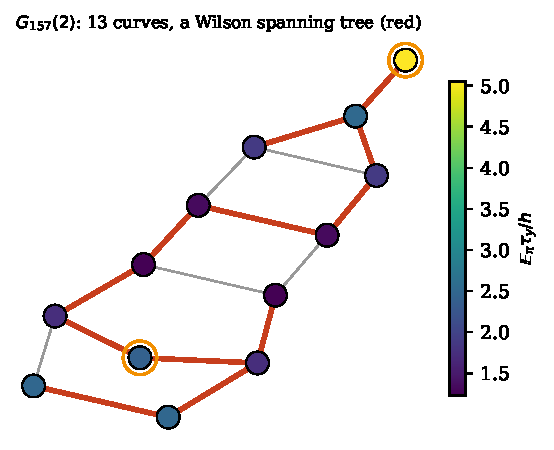
\includegraphics[width=0.72\textwidth]{figs/hit_graph.pdf}
\caption{The supersingular $2$ isogeny graph $G_{157}(2)$ (edge width is multiplicity, circles mark the two curves with loops), coloured by $\E_\pi\tau_y/h$ (Proposition~\ref{prop:hitvertex}), with a uniform spanning tree sampled by Wilson's algorithm in red. The graph has $|J_0(157)(\mathbb F_2)|/13=1418$ spanning trees.}\label{fig:hitgraph}
\end{figure}

\subsection{Data}

We built the isogeny walks from modular polynomials over $\mathbb F_{N^2}$, as in Section~\ref{sec:B:ssgraph}, for $\ell\in\{2,3,5,7\}$, the $49$ primes $N\equiv1\bmod12$ below $1300$, and the nine primes $11,23,43,47,59,71,83,107,131$, which are not $1$ modulo $12$, and computed $T_\ell$ on $S_2(\Gamma_0(N))$ independently with modular symbols in PARI/GP. Kemeny's constant of the walk, computed from the spectrum of $P$, agrees with the sum in Theorem~\ref{thm:hitkemeny} to relative error below $2\cdot10^{-14}$ in all $228$ cases with $g\ge1$, including the levels with extra automorphisms; computed in rational arithmetic from the Laplacian, it equals the sum exactly in the $108$ cases with $N\equiv1\bmod12$ below $700$. In all $196$ cases with $N\equiv1\bmod12$ the exact integer determinant of the reduced Laplacian times $h$ equals $|J_0(N)(\mathbb F_\ell)|$, computed as the characteristic polynomial of $T_\ell$ evaluated at $\ell+1$; the largest, for $N=1297$ and $\ell=7$, has $94$ digits. The Kirchhoff index agrees with Theorem~\ref{thm:hitresist} to $6\cdot10^{-16}$. Figure~\ref{fig:hitisogeny} shows $g^{-1}\log|J_0(N)(\mathbb F_\ell)|$ approaching the tree entropy, from above for $\ell=5$ and $7$; for $\ell=2$ three of the $48$ levels with $g\ge2$, and for $\ell=3$ eight, lie below it, by at most $0.02$. At $N=1297$ the values are $0.8566$, $1.2249$, $1.6973$ and $2.0187$.

\begin{figure}[t]
\centering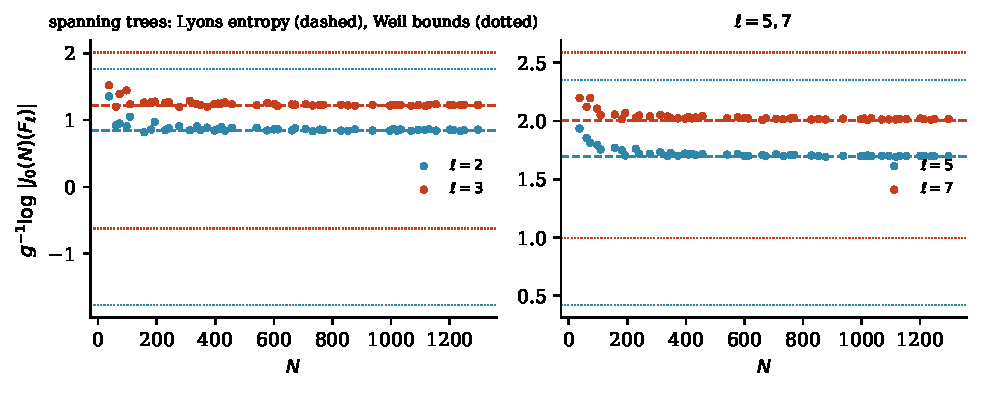
\includegraphics[width=\textwidth]{figs/hit_isogeny.pdf}
\caption{Theorems~\ref{thm:hittrees} and \ref{thm:hitentropy}: $g^{-1}\log|J_0(N)(\mathbb F_\ell)|$, which equals $g^{-1}\log(h\,\tau(G_N(\ell)))$, for primes $N\equiv1\bmod12$ below $1300$, against the spanning tree entropy of the $(\ell+1)$ regular tree (dashed) and the Weil bounds $2\log(\sqrt\ell\pm1)$ (dotted).}\label{fig:hitisogeny}
\end{figure}

\section{Chebotarev densities are hitting rates}\label{sec:hitrate}

Return to the zeta random integer $N_\sigma$ of Section~\ref{sec:recipgammaproc}, with prime factors labelled by Frobenius classes or Satake parameters $\theta_p\in Y$, equidistributed with respect to $\mu$. Scan the prime factors from the largest down. For a Borel set $B\subset Y$ let $P_B^+$ be the largest prime factor of $N_\sigma$ with label in $B$, and $V_B=(\sigma-1)\log P_B^+$ ($V_B=0$ if there is none). Write $E_1(v)=\int_v^\infty e^{-x}x^{-1}dx$ for the exponential integral.

\begin{theorem}[hitting rates; after Lloyd \cite{lloyd1984}]\label{thm:hitrate}
Let $B$ be a $\mu$ continuity set. As $\sigma\downarrow1$:
\begin{enumerate}
\item[(i)] $\Prob(V_B\le v)\to\exp(-\mu(B)E_1(v))$ for every $v>0$; if $\mu(B)>0$, equivalently, $E_1(V_B)$ converges in law to the exponential law with rate $\mu(B)$, and if $\mu(B)=0$, then $V_B\to0$ in probability;
\item[(ii)] the label of the largest prime factor of $N_\sigma$ lies in $B$ with probability tending to $\mu(B)$, and the labels of the $k$ largest prime factors are asymptotically independent with law $\mu$, independent of their sizes;
\item[(iii)] for two continuous functions $a$ and $b$ on $Y$, such as the characters $\chi_\rho$ and $\chi_{\rho'}$ of Theorem~\ref{thm:recipthorin}(a), whose discrepancy set $D=\{a\ne b\}$ is a $\mu$ continuity set, (i) holds for $B=D$, and $\mu(D)$ is the mass of the Thorin measure $\tau_Q$ of Theorem~\ref{thm:recipggcfun} for $Q=|a-b|^2$; in particular $V_D\to0$ in probability if and only if $\tau_Q=0$.
\end{enumerate}
\end{theorem}

\begin{proof}
By Theorem~\ref{thm:recipgammaproc}(i) the rescaled sizes and labels of the prime factors converge to the Poisson process with intensity $x^{-1}e^{-x}dx\otimes\mu$. Prime factors with $e_p\ge2$ give no point above a fixed level $v>0$ in the limit, since $\sum_{e\ge2}\sum_{p^e>\exp(v/(\sigma-1))}p^{-e\sigma}\to0$, so the points $((\sigma-1)\log p,\theta_p)$ have the same limit. The event $\{V_B\le v\}$ is the event that this process has no point in $(v,\infty)\times B$, whose mean number of points is $\mu(B)E_1(v)$; points beyond a large level $M$ are excluded with probability at least $1-E_1(M)-o(1)$, uniformly in $\sigma$, because the expected number of prime factors $p$ of $N_\sigma$ with $(\sigma-1)\log p>M$ is at most $\sum_{(\sigma-1)\log p>M}p^{-\sigma}(1-p^{-\sigma})^{-1}\to E_1(M)$. This gives (i), and (ii) follows from the independence of labels and sizes in the limiting Poisson process. For (iii) apply (i) to $B=D$; the Thorin mass is $\mu(D)$ by Theorem~\ref{thm:recipggcfun}.
\end{proof}

So Chebotarev's density is literally a hitting rate: in the logarithmic integral scale $E_1$, the first prime factor (from the top) whose Frobenius lies in $C$ arrives after an exponential time with rate $|C|/|G|$. Reciprocity laws are statements that a discrepancy set is hit at rate zero. For a prime $q\equiv3\bmod4$, omitting the factor $(\frac{-1}p)$ from quadratic reciprocity gives a discrepancy set that is hit at rate $\frac12$; the pair $(\rho,\rho_{31})$ of $S_3$ representations of Chapter~\ref{ch:recip} has discrepancy rate $\frac{11}{18}$.

For the $S_3$ field of $x^3-x-1$ the probability that the largest prime factor of $N_\sigma$ outside the set $S=\{2,7,11,23,31,37\}$ of the example after Theorem~\ref{thm:recipdrift} has Frobenius in a given class, conditional on there being such a factor, was computed exactly from the primes below $10^7$, with larger primes from the prime number theorem (at $\sigma=1.005$ the largest prime factor exceeds $10^7$ with probability $0.87$, and its class is then given the limit law). At $\sigma=1.005$ it is $0.1626$, $0.5000$ and $0.3375$ for the identity, the transpositions and the three cycles, against $\frac16$, $\frac12$, $\frac13$; at $\sigma=1.5$ it is $0.021$, $0.392$ and $0.587$, so at moderate $\sigma$ small primes still dominate (Figure~\ref{fig:hitrates}). To first order the approach is linear in $\sigma-1$, with slope $s_C=\sum_{p\notin S}\bigl(\mathsf 1_C(\Frob_p)-\mu(C)\bigr)p^{-1}\prod_{p'\le p\text{ or }p'\in S}(1-1/p')^{-1}$, a Chebotarev bias weighted by Mertens products; for the primes below $10^7$, $s_C=-0.835$, $0.003$ and $0.832$, so the transpositions converge fastest. For Chebotarev labels and a uniform random integer below $x$, the class of a size biased prime factor approaches Haar measure at rate $1/\log x$, the class of the largest one faster still, but the classes of the distinct prime factors only at rate $1/\log\log x$ (Chapter~\ref{ch:pd}).

\begin{figure}[t]
\centering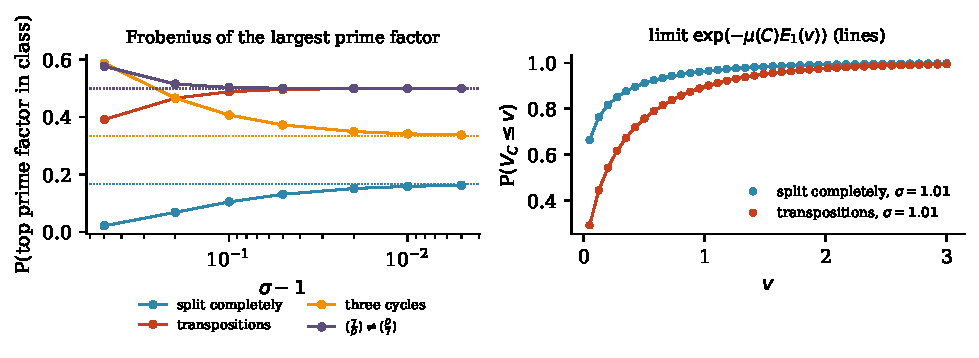
\includegraphics[width=0.72\textwidth,trim=0 0 234 0,clip]{figs/hit_rates.pdf}
\caption{Theorem~\ref{thm:hitrate} for the $S_3$ field of $x^3-x-1$: the probability that the largest prime factor of $N_\sigma$ outside $S$ has Frobenius in a given class, conditional on one existing, and that it lies in the discrepancy set $\{p:(\frac7p)\ne(\frac p7)\}$, against $\sigma-1$, with their limits (dotted).}\label{fig:hitrates}
\end{figure}

\section{Explosion times and the Thorin converse theorem}\label{sec:hitexplosion}

A pure birth process on $\{0,1,2,\dots\}$ started at $0$ with rates $u_1\le u_2\le\dots$, repetitions allowed, spends independent exponential times with means $1/u_k$ in successive states. If $\sum_k1/u_k<\infty$ it explodes at the finite time
\[
T=\sum_k\frac{\mathcal E_k}{u_k},\qquad \E e^{-sT}=\prod_k\Bigl(1+\frac s{u_k}\Bigr)^{-1},
\]
with $\mathcal E_k$ independent standard exponentials. So explosion laws are exactly the GGCs with zero drift whose Thorin measure is a sum of unit point masses: atomic Thorin measures with \emph{integer} masses. This is the integrality condition in Theorem~\ref{thm:recipeuler}, now with a meaning: multiplicities of zeros are repeated birth rates.

\begin{theorem}[explosion times; after Theorem~\ref{thm:10dduality}]\label{thm:hitexplosion}
Let $\Lambda(s)$ be entire of order at most one with $\Lambda(s)=\Lambda(1-s)$ and $\Lambda(\frac12)\ne0$, and write its zeros as $\frac12\pm i\gamma_k$, with multiplicity. The following are equivalent.
\begin{enumerate}
\item[(i)] Every $\gamma_k$ is real.
\item[(ii)] There is a generalized gamma convolution $T$ with $\E e^{-sT}=\Lambda(\frac12)/\Lambda(\frac12+\sqrt s)$ for all $s>\frac14$.
\item[(iii)] $\Lambda(\frac12)/\Lambda(\frac12+\sqrt s)$, $s>\frac14$, is the Laplace transform of the explosion time of a pure birth process.
\end{enumerate}
In that case the birth rates are the $\gamma_k^2$, $T$ is infinitely divisible with L\'evy density $\mathcal W(x)/x$, where $\mathcal W(x)=\sum_{\gamma_k>0}e^{-x\gamma_k^2}$ is the heat trace, and the cumulants of $T$ are
\[
\begin{gathered}
\kappa_m(T)=(m-1)!\sum_k\gamma_k^{-2m}=\int_0^\infty x^{m-1}\mathcal W(x)\,dx,\\
\E T=\sum_k\frac1{\gamma_k^2}=\frac12\,\frac{\Lambda''}{\Lambda}\Bigl(\frac12\Bigr).
\end{gathered}
\]
\end{theorem}

\begin{proof}
For real $\Lambda$ with $\Lambda(\frac12)>0$, the equivalence of (i) and (ii) and the Thorin measure $\sum_k\delta_{\gamma_k^2}$ are Theorem~\ref{thm:10dduality} with $f=\Lambda$ and $\alpha=\frac12$, and the variable in (iii) is that of Theorem~\ref{thm:10babstract}(c); the argument is short, and we repeat it without these hypotheses. By Hadamard, $\Lambda(\frac12+z)/\Lambda(\frac12)$ is an even entire function of order at most one, so it equals $\prod_k(1+z^2/\gamma_k^2)$ with $\sum|\gamma_k|^{-2}<\infty$, the exponential factor being trivial by evenness. If (i) holds, (iii) holds with rates $\gamma_k^2$, and an explosion time is a GGC with Thorin measure $\sum_k\delta_{\gamma_k^2}$, so (iii) implies (ii). Conversely let $T$ be a GGC with drift $a$ and Thorin measure $\tau$ as in (ii). Taking logarithms and differentiating in $s$,
\[
a+\int\frac{\tau(dt)}{t+s}=\sum_k\frac1{\gamma_k^2+s},\qquad s>\tfrac14 .
\]
The left side is analytic on $\C\setminus(-\infty,0]$, and the right side is meromorphic on $\C$ with a pole at each $-\gamma_k^2$. So every $\gamma_k^2$ lies in $[0,\infty)$, and $\gamma_k^2\ne0$ because $\Lambda(\frac12)\ne0$: every $\gamma_k$ is real. (Letting $s\to\infty$ shows $a=0$, and comparing residues shows $\tau=\sum_k\delta_{\gamma_k^2}$, as in Theorem~\ref{thm:recipeuler}.) For the L\'evy density, Frullani's integral gives $\sum_k\log(1+s/\gamma_k^2)=\int_0^\infty(1-e^{-sx})\mathcal W(x)x^{-1}dx$. The cumulants follow by differentiating at $s=0$, or from $\int_0^\infty x^{m-1}e^{-x\gamma^2}dx=(m-1)!\gamma^{-2m}$, and $\Lambda''/\Lambda(\frac12)=2\sum_k\gamma_k^{-2}$ from the product.
\end{proof}

The hypothesis in (ii) cannot be weakened to positivity of $T$. With $w=2+i$, the function $1/((1+s)(1+s/w)(1+s/\bar w))$ is the Laplace transform of the probability density $\frac52e^{-t}\bigl(1-e^{-t}(\cos t+\sin t)\bigr)$ on $(0,\infty)$, which is nonnegative because $e^{-t}(\cos t+\sin t)$ decreases on $[0,\pi]$ and is at most $\sqrt2e^{-\pi}<1$ beyond, although two of its poles are not real. What the GGC property adds is positivity of the Thorin measure, which forces the poles onto the negative axis.

The mean explosion time is a number computed from Galois data. By Definition~\ref{def:recipheat} the heat trace $\mathcal W$ is given by the explicit formula from the prime powers, the conductor and the gamma factor, and $\E T=\int_0^\infty\mathcal W(x)\,dx$. Under GRH this integral is the mean of a positive random variable, the explosion time whose birth rates are the squared ordinates $\gamma_k^2$ of the zeros. For $\xi$, for $L(s,\Delta)$ in the unitary normalisation and for the $S_3$ representation $\rho$ of $x^3-x-1$, of conductor $23$, the sum $\sum_k\gamma_k^{-2}$ is the constant $S_1$ of Table~\ref{tab:10bcatalogue}, $0.023105$, $0.0561759$ and $0.170287$, computed there from the central Taylor coefficients and checked against the zeros.

The mean explosion time can also be computed from the Frobenius classes, the conductor and the gamma factor, with no analytic continuation; only the tail of the integral needs a bound on the zeros. For the $S_3$ representation $\rho$ we evaluated the Galois heat trace of Definition~\ref{def:recipheat} from the Frobenius classes of $x^3-x-1$ at the $664579$ primes below $10^7$ and their powers below $10^7$, with the archimedean integral by quadrature. It agrees with $\sum e^{-x\gamma^2}$ over the zeros to fifteen digits at $x=0.001$, $0.005$, $0.02$ and $0.1$. Integrating over $e^{-60}\le x\le1.1$ (beyond which $\mathcal W<e^{-28}$, by the first zero $\gamma_1=5.1157$) gives
\[
\int_{e^{-60}}^{1.1}\mathcal W(x)\,dx=0.17028731076215,
\]
against $0.17028731076373$ from the Hadamard product, a difference of $1.6\cdot10^{-12}$ that the integral over the two omitted ends accounts for to $3\cdot10^{-17}$. Since $L(s,\rho)$ is entire, $\rho$ being dihedral, the explicit formula gives $\mathcal W(x)=\sum_ke^{-x\gamma_k^2}$ unconditionally. If GRH holds for $L(s,\rho)$, which is not known, $\sum_k\gamma_k^{-2}$ is the mean explosion time of a birth process whose rates are the squared ordinates of the zeros, and it has been computed from the factorisation of $x^3-x-1$ modulo primes (which determines the Frobenius class in $S_3$), the conductor $23$ and the gamma factor. The agreement does not verify GRH: a finite computation of this kind can disprove it and is not known to verify it.

Combining Theorem~\ref{thm:hitexplosion} with Corollary~\ref{cor:recipconverse} gives an explosion form of the Thorin converse theorem.

\begin{corollary}[Thorin converse theorem as explosion; this book]\label{cor:hitconverse}
Let $k\equiv0\bmod4$ and let $(a_p)$ be the Frobenius traces of a self dual Galois representation of conductor $1$ with the gamma factor $\Gamma_\C(s+\frac{k-1}2)$ of Corollary~\ref{cor:recipconverse} and the Ramanujan bound, and $\Lambda$ its completion, defined on $\operatorname{Re}s>1$ by the Euler product. If for some constant $c>0$ the function $c/\Lambda(\frac12+\sqrt s)$, $s>\frac14$, is the Laplace transform of the explosion time $T$ of a pure birth process, then $f=\sum a_nn^{(k-1)/2}q^n$ is a cusp form for $\SL_2(\Z)$ satisfying GRH, and $c=\Lambda(\frac12)\ne0$. Conversely, if $f$ is such a cusp form satisfying GRH with $\Lambda(\frac12)\ne0$, this holds with $c=\Lambda(\frac12)$. If moreover the P\'olya kernel $\Phi_f$ is nonnegative, as for $\Delta$ (but not for one of the two eigenforms of weight $24$), then the P\'olya variable $W_f$ and $T$ form a Wald couple: $\E e^{tW_f}\,\E e^{-t^2T}=1$ for all real $t$.
\end{corollary}

\begin{proof}
Explosion laws are exactly the GGCs with integer atomic Thorin measures. Under the hypothesis, $\Lambda(\frac12+\sqrt{s_0})/\Lambda(\frac12+\sqrt s)$ is $c^{-1}\Lambda(\frac12+\sqrt{s_0})$ times the Laplace transform of such a GGC, so Corollary~\ref{cor:recipconverse} gives the cusp form and GRH; then $\Lambda(\frac12+z)=c\prod_k(1+z^2/u_k)$ and $z=0$ gives $c=\Lambda(\frac12)$. The converse is Theorem~\ref{thm:hitexplosion}. For the Wald couple, $\E e^{tW_f}=\Lambda(\frac12+t)/\Lambda(\frac12)$ for every real $t$, by \eqref{eq:recipmellin} (whose classical completion at $\frac k2+t$ is a constant times $\Lambda(\frac12+t)$) and the doubly exponential decay of $\Phi_f$, and $\E e^{-t^2T}=\prod_k(1+t^2/\gamma_k^2)^{-1}=\Lambda(\frac12)/\Lambda(\frac12+t)$ by the Hadamard product; this is the Wald couple of Theorem~\ref{thm:10dvdp}(c).
\end{proof}

As with Corollary~\ref{cor:recipconverse}, the hypothesis contains GRH, so it is stronger than reciprocity. Keilson's theorem (Theorem~\ref{thm:10ckeilson}) and Kent's extension to diffusions \cite{kent1980} go the other way: first passage times of birth death chains and of diffusions have laws of this form, with rates from their spectra, and whether a given law is such a passage time is an inverse spectral question. The pure birth realisation needs no simplicity of the zeros and is the one that matches the integrality in the Thorin converse theorem.

\section{Brownian exit and the functional equation of odd characters}\label{sec:hitexit}

The functional equations of even Dirichlet $L$ functions came in Section~\ref{sec:recipgauss} (Theorem~\ref{thm:recipdirichlet}) from the wrapped normal law. For odd characters the natural object is the exit of Brownian motion from an interval, and the signed starting distribution is the character itself.

Let $q\ge3$, let $B$ be standard Brownian motion started at $r\in(0,q)$, let $\tau$ be its exit time from $(0,q)$, and let $f_r^0(t)$ and $f_r^q(t)$ be the densities of $\tau$ on the events of exit at $0$ and at $q$.

\begin{theorem}[signed exit law; after Biane, Pitman and Yor \cite{bpy2001}]\label{thm:hitexit}
Let $\chi$ be an odd primitive character modulo $q$ and $g(\chi)=\sum_r\chi(r)e^{2\pi ir/q}$. For every $t>0$,
\[
\begin{split}
\sum_{r=1}^{q-1}\chi(r)\bigl(f_r^0(t)-f_r^q(t)\bigr)&=\frac2{\sqrt{2\pi t^3}}\sum_{m\ge1}\chi(m)\,m\,e^{-m^2/(2t)}\\
&=-\frac{4\pi i\,g(\chi)}{q^2}\sum_{j\ge1}\bar\chi(j)\,j\,e^{-2\pi^2j^2t/q^2}.
\end{split}
\]
Consequently $\vartheta_\chi(x)=\sum_{n\ge1}\chi(n)\,n\,e^{-\pi n^2x/q}$ satisfies
\[
\vartheta_\chi(1/x)=\frac{g(\chi)}{i\sqrt q}\,x^{3/2}\,\vartheta_{\bar\chi}(x),
\]
and $\Lambda(s,\chi)=(q/\pi)^{(s+1)/2}\Gamma(\frac{s+1}2)L(s,\chi)$ satisfies $\Lambda(s,\chi)=\frac{g(\chi)}{i\sqrt q}\Lambda(1-s,\bar\chi)$.
\end{theorem}

\begin{proof}
The method of images (the reflection principle) gives
\[
\begin{aligned}
f_r^0(t)&=\sum_{n\in\Z}\frac{r+2nq}{\sqrt{2\pi t^3}}e^{-(r+2nq)^2/(2t)},\\
f_r^q(t)&=\sum_{n\in\Z}\frac{q-r+2nq}{\sqrt{2\pi t^3}}e^{-(q-r+2nq)^2/(2t)} .
\end{aligned}
\]
In the first sum $m=r+2nq$ runs over the integers $\equiv r\bmod 2q$ and $\chi(r)=\chi(m)$. In the second $m=q-r+2nq\equiv-r\bmod q$, so $\chi(r)=-\chi(m)$ because $\chi$ is odd. Hence $\sum_r\chi(r)(f_r^0-f_r^q)=2(2\pi t^3)^{-1/2}\sum'\chi(m)me^{-m^2/2t}$, the sum over all integers $m$ whose residue modulo $2q$ lies in $(0,q)$. For negative $m$ put $m'=-m$; then $m'\bmod2q\in(q,2q)$ and $\chi(m)m=\chi(m')m'$. The two ranges together cover every positive integer prime to $q$ once, which is the first identity. The eigenfunction expansion of the killed heat kernel gives
\[
f_r^0(t)-f_r^q(t)=\sum_{k\ge1}\frac{k\pi}{q^2}\bigl(1+(-1)^k\bigr)\sin\frac{k\pi r}q\,e^{-k^2\pi^2t/(2q^2)},
\]
since exit at $q$ from $r$ is exit at $0$ from $q-r$, and $\sin(k\pi(q-r)/q)$ equals $(-1)^{k+1}\sin(k\pi r/q)$. Only $k=2j$ survives, and for odd primitive $\chi$,
\[
\sum_r\chi(r)\sin\frac{2\pi jr}q=\frac1{2i}\bigl(\bar\chi(j)-\bar\chi(-j)\bigr)g(\chi)=-i\,\bar\chi(j)g(\chi).
\] This is the second identity. Putting $t=qx/(2\pi)$ and comparing gives the transformation of $\vartheta_\chi$, and the Mellin transform $\int_0^\infty\vartheta_\chi(x)x^{(s+1)/2}dx/x=\Lambda(s,\chi)$ gives the functional equation in the usual way.
\end{proof}

The root number $g(\chi)/(i\sqrt q)$ is the eigenfunction weight of the signed starting law, the Fourier coefficient of $r\mapsto\chi(r)$ against the sine modes of the interval. For a real odd character modulo a prime $q\equiv3\bmod4$ it is $1$, which is Gauss's sign $g(\chi)=g(q)=i\sqrt q$ of Corollary~\ref{cor:recipgausssign}. For $q=4$, $\chi=\chi_{-4}$, the theorem is the reciprocal law of the exit time of Brownian motion started at the centre of an interval, which Biane, Pitman and Yor \cite{bpy2001} credit to Ciesielski and Taylor \cite{ciesielskitaylor1962} and from which they obtained the functional equation of Dirichlet's $\beta$ function; Salminen and Vignat \cite{salminenvignat2024} derive it by comparing the image and eigenfunction expansions, as here. For real odd characters Biane, Pitman and Yor wrote the Laplace transform of $\vartheta_\chi$, using the classical transformation formula, as a combination with weights $\chi(n)$ of ratios of hyperbolic sines, which are Laplace transforms of Brownian exit laws from an interval, and observed, after P\'olya, that $\vartheta_\chi$ need not be positive, while its positivity would exclude a real zero of $L(s,\chi)$ (\cite{bpy2001}, Section~6.1). Theorem~\ref{thm:hitexit} reads that combination as an exit law whose starting point is spread over the interval with the character as a signed weight, and reverses the argument: the transformation formula follows by comparing the image and eigenfunction expansions. For $\chi_{-4}$ the function $\vartheta_\chi$ is positive, since $\vartheta_{\chi_{-4}}(x)=\eta(ix)^3$ by Jacobi's identity (Proposition~\ref{beta:prop:kernel}). For the character $\chi_d$ of an imaginary quadratic field $K$ of discriminant $d$, the completed Dedekind zeta function of $K$ is a constant multiple of $\xi(s)\Lambda(s,\chi_d)$, so its P\'olya kernel (Theorem~\ref{thm:sf:kernel}) is a positive multiple of the convolution of P\'olya's kernel of $\xi$ with $v\mapsto e^{3v/2}\vartheta_{\chi_d}(e^{2v})$; hence, by Theorem~\ref{thm:sf:inert}, $\vartheta_{\chi_d}$ takes negative values whenever $2$ and $3$ are inert in $K$, that is whenever $d\equiv5\bmod24$. In $40$ digit arithmetic, for $\chi_{-3}$, $\chi_{-4}$, $\chi_{-7}$, $\chi_{-8}$, the odd character modulo $5$ with $\chi(2)=i$ and an odd character of order $6$ modulo $7$ at $t=0.3$, $1$ and $3$, the image and eigenfunction sums agree with each other and with both closed forms to $10^{-40}$; Figure~\ref{fig:hitexit} plots four of these characters.

\begin{figure}[t]
\centering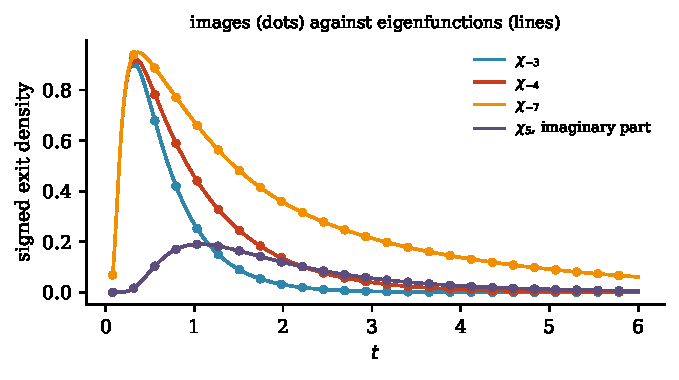
\includegraphics[width=0.72\textwidth]{figs/hit_exit.pdf}
\caption{Theorem~\ref{thm:hitexit} for $\chi_{-3}$, $\chi_{-4}$, $\chi_{-7}$ and the odd character modulo $5$ with $\chi(2)=i$ (imaginary part, labelled $\chi_5$): the two closed forms of the signed exit density, the image sum (dots) and the eigenfunction sum with the Gauss sum as weight (lines).}\label{fig:hitexit}
\end{figure}

\section{A dictionary}\label{sec:hitdictionary}

The correspondences of the chapter, side by side.

\begin{center}\small
\begin{tabular}{p{0.44\textwidth}p{0.46\textwidth}}
\toprule
Hitting time & Reciprocity\\
\midrule
Kemeny constant of the isogeny walk mod $N$ & harmonic sum of the factors $\ell+1-a_\ell(f)$ of $|J_0(N)(\mathbb F_\ell)|$\\
spanning trees ($N\equiv1\bmod12$) & $|J_0(N)(\mathbb F_\ell)|/|J_0(N)(\Q)_{\mathrm{tors}}|$\\
critical group ($N\equiv1\bmod12$) & order $|J_0(N)(\mathbb F_\ell)|/h$; $r$ part $\mathbb T_r/(\ell+1-T_\ell)\mathbb T_r$ for $r\nmid\ell hN$ prime to the discriminant of $\mathbb T$ (Proposition~\ref{prop:hitsandpile})\\
tree entropy of $\T_\ell$ & growth of $|J_0(N)(\mathbb F_\ell)|$\\
bounds on hitting times and spanning trees & Weil bound for $a_\ell(f)$\\
hitting rate of a class by top prime factors & Chebotarev density\\
discrepancy set hit at rate zero & reciprocity, vanishing Thorin mass\\
explosion time of a pure birth process & Thorin converse theorem, GRH\\
mean explosion time & $\int\mathcal W$, computable from Frobenius data, conductor and gamma factor\\
signed exit law, images against eigenfunctions & functional equation of odd $L(s,\chi)$\\
\bottomrule
\end{tabular}
\end{center}

\subsection{Open problems}

\begin{problem}[Sandpile groups and Jacobians]\label{op:hitsandpile}
Fix $\ell$ and let $N\to\infty$ through primes $N\equiv1\bmod12$. Find the limiting law of the $r$ part of the critical group of $G_N(\ell)$, a question Munier and Shnidman raise \cite{muniershnidman2023}. By Proposition~\ref{prop:hitsandpile}, for $r\ne\ell$ prime to $hN$ and to the discriminant of $\mathbb T$, it is governed by the valuations of $\ell+1-a_\ell(f)$ at the primes above $r$ of the Hecke fields, so, as Munier and Shnidman note, it needs an $r$ adic analogue of the vertical equidistribution of Theorem~\ref{thm:07serre}. For the primes $r$ dividing $h$ or the discriminant of $\mathbb T$, which Proposition~\ref{prop:hitsandpile} excludes, describe the critical group, and decide when the class of $L\delta_E$ corresponds to the cuspidal subgroup $C_N$. Extend the comparison to $\ell=2$ and to levels $N\not\equiv1\bmod12$, where the graph is weighted by automorphisms.
\end{problem}

\begin{problem}[Vertex hitting times and Gross's formula]\label{op:hitgross}
By Exercise~\ref{ex:hitgross}, Gross's formula turns the mean $\sum_{x,y}c_xc_y\E_x\tau_y$ of hitting times between the reductions of the curves with complex multiplication by discriminant $D$, less its stationary part $(\deg e_D)\sum_yc_y\E_\pi\tau_y$, into a combination of the central values $L(f,1)L(f\otimes\chi_D,1)$ over the newforms of level $N$. For fixed $N$ and $\ell$, find the distribution of this combination over $D$, a question about the central values of the quadratic twists of the newforms of level $N$. Find also the law of the hitting time of the support of $e_D$ from stationarity, and decide which arithmetic quantities it computes: its Laplace transform involves the values $\phi_f(x)\overline{\phi_f(y)}$ at pairs of points of the support, not only the linear forms $\sum_yc_y\phi_f(y)$ of Gross's formula.
\end{problem}

\section{Notes}

The supersingular isogeny graph and Brandt matrices are in Deuring, Eichler, Mestre, Gross and Pizer \cite{deuring1941,eichler1954,mestre1986,gross1987,pizer1990}; the congruence relation is Eichler and Shimura \cite{shimura1971}; rational torsion of $J_0(N)$ is Ogg's conjecture proved by Mazur \cite{ogg1975,mazur1977}, and injectivity of reduction on torsion is in Katz \cite{katz1981}. Kemeny's constant is from \cite{kemenysnell1960}, the matrix tree theorem is Kirchhoff's \cite{kirchhoff1847}, critical groups are in Biggs \cite{biggs1997} and Baker and Norine \cite{bakernorine2007}, uniform spanning trees from random walks in Aldous, Broder and Wilson \cite{aldous1990,broder1989,wilson1996}, resistances in Doyle and Snell \cite{doylesnell1984}, the Kirchhoff index in \cite{gutmanmohar1996,zhukleinlukovits1996} and the commute time identity in \cite{chandra1996}. McKay \cite{mckay1983} computed the asymptotic number of spanning trees of regular graphs with large girth and Lyons \cite{lyons2005} the tree entropy. The vertical Sato Tate theorem is Serre's \cite{serre1997}. Explosion of pure birth processes is classical (Feller \cite{feller1968}, Section XVII.4), Keilson's theorem is \cite{keilson1971}, Kent's is \cite{kent1980}. The tree count of Theorem~\ref{thm:hittrees} is Hashimoto's formula \cite[(7.14)]{hashimoto1989}, presented by Li \cite[Section~4.3]{li2019}; Munier and Shnidman \cite{muniershnidman2023} sketch the proof given here, call the formula a kind of reciprocity law between the Jacobian of the graph and that of $X_0(N)$, prove Proposition~\ref{prop:hitcritical} and the first statement of Proposition~\ref{prop:hitsandpile}, note the cuspidal point behind Corollary~\ref{cor:hittorsion}, and find the laws of the $r$ parts of the critical groups for fixed $N$ and $r\nmid6h$ prime to the discriminant of $\mathbb T$, as $\ell\to\infty$. The limit in Theorem~\ref{thm:hitentropy} is an asymptotic class number of Tsfasman and Vl\u{a}du\c{t} \cite{tsfasmanvladut2002}. For one label, Theorem~\ref{thm:hitrate}(i) is Lloyd's limit law for the largest prime factor \cite{lloyd1984}, and Theorem~\ref{thm:hitexplosion} restates Theorems~\ref{thm:10babstract} and \ref{thm:10dduality}. Theorem~\ref{thm:hitexit} is after Biane, Pitman and Yor \cite{bpy2001}, as explained after it, and the transformation formula is classical (\cite{bump1997}, Section~1.1). Deriving theta transformations from the heat equation goes back at least to Bellman \cite{bellman1961}, for $\vartheta_3$, and Salminen and Vignat \cite{salminenvignat2024} derive the modular identities of the Jacobi theta functions by comparing the image and eigenfunction expansions of the heat kernels of an interval, among them the case $q=4$ of Theorem~\ref{thm:hitexit}, the exit time from the centre. Ours are Theorems~\ref{thm:hitkemeny} and \ref{thm:hitresist} in the forms stated (for $N\equiv1\bmod12$ the Kemeny formula is the expression in the proof of Theorem~\ref{thm:08kemeny}), the isomorphism criterion of Proposition~\ref{prop:hitsandpile}, the reading of the limit in Theorem~\ref{thm:hitentropy} as a tree entropy, the labelled form of Theorem~\ref{thm:hitrate}, the explosion reading of Theorem~\ref{thm:hitexplosion}, the extension of the image and eigenfunction derivation to every odd primitive character through the signed exit law of Theorem~\ref{thm:hitexit}, Corollaries~\ref{cor:hithasse} and \ref{cor:hitconverse}, and the computations; each is a short consequence of the cited theory, and none proves a new case of reciprocity, of Artin's conjecture or of GRH.

\section{Exercises}

\begin{enumerate}
\item Compute $G_{11}(2)$ and $G_{11}(3)$ from $\Phi_2$ and $\Phi_3$ over $\mathbb F_{121}$, with the weights $w$ of $j=0$ and $j=1728$, and check $K_{11}(2)=\frac35$, $K_{11}(3)=\frac45$ against $|11a1(\mathbb F_2)|=|11a1(\mathbb F_3)|=5$.
\item For $N=37$ and $\ell=2$, draw the three vertex graph, list its five spanning trees and compute all hitting times. Compare with Proposition~\ref{prop:hitvertex}.
\item Show that the Laplace transform of the explosion time of a pure birth process determines the multiset of rates, and deduce that Corollary~\ref{cor:hitconverse} recovers the zeros with multiplicity.
\item Check Theorem~\ref{thm:hitexit} for $\chi_{-3}$ by computing the image sum and the eigenfunction sum at $t=1$ to ten digits, verify $g(\chi_{-3})=i\sqrt3$, and derive the functional equation of $L(s,\chi_{-3})$ from the transformation of $\vartheta_{\chi_{-3}}$.
\item Show that $\E[(\sigma-1)\log P^+(N_\sigma)]\to\int_0^\infty x\cdot\frac{d}{dx}e^{-E_1(x)}dx$, where $P^+$ is the largest prime factor ($P^+(1)=1$), and that the limit is the Golomb Dickman constant $\int_0^\infty e^{-x-E_1(x)}dx=0.62433\ldots$ (Lloyd \cite{lloyd1984}; for uniform integers, Theorem~\ref{thm:pdbillingsley}). To pass from convergence in law to convergence of means, bound $\E[V;V>M]$, for $V=(\sigma-1)\log P^+(N_\sigma)$, by the expected sum of $(\sigma-1)\log p$ over the prime factors $p$ with $(\sigma-1)\log p>M$, which tends to $e^{-M}$.
\item\label{ex:hitgross} Let $N\equiv1\bmod12$, let $D<0$ be a fundamental discriminant with $N$ inert in $\Q(\sqrt D)$, and let $e_D=\sum_yc_y[E_y]$ be the divisor of Gross's formula \cite{gross1987}, whose coefficient $c_y$ counts the curves with complex multiplication by the ring of integers of $\Q(\sqrt D)$ that reduce to $E_y$. With $\phi_f$ as in Proposition~\ref{prop:hitvertex}, show that
\[
\sum_{x,y}c_xc_y\E_x\tau_y=(\deg e_D)\sum_yc_y\E_\pi\tau_y-(\ell+1)\sum_f\frac{\bigl|\sum_yc_y\phi_f(y)\bigr|^2}{\ell+1-a_\ell(f)},
\]
using $\E_x\tau_y=(Z(y,y)-Z(x,y))/\pi(y)$ (Theorem~\ref{thm:A:kemeny}), and deduce from Gross's formula that the last sum is a combination of the $L(f,1)L(f\otimes\chi_D,1)/(\ell+1-a_\ell(f))$ with positive coefficients that do not depend on $\ell$.
\item\label{ex:hitnonback} Show that the nonbacktracking walk on a connected $(q+1)$ regular graph on $n$ vertices without half loops, $q\ge2$, has Kemeny constant $(n-1)+\frac{q-1}{q+1}K+\frac q{q-1}+\frac{nq^2}{q+1}$, where $K$ is the Kemeny constant of the simple walk (use the Ihara Bass formula of Chapter~\ref{ch:08}). When $G_N(\ell)$ has no half loops, write it with Theorem~\ref{thm:hitkemeny} as a sum over the factors $\ell+1-a_\ell(f)$ of $|J_0(N)(\mathbb F_\ell)|$.
\end{enumerate}

\section{Open computational problems}

\begin{compproblem}[Two prime tables]\label{cp:hittables}
Objective: for fixed $\ell$ and small primes $r\ne\ell$, the empirical law of the $r$ part of the critical group of $G_N(\ell)$ over the primes $N\equiv1\bmod12$, against the Haar model that Munier and Shnidman prove for fixed $N$ and $\ell\to\infty$ and against the Cohen Lenstra law of Chapter~\ref{ch:06c} (Open Problem~\ref{op:hitsandpile}), with the frequency of noncyclic $r$ parts of $J_0(N)(\mathbb F_\ell)$. Objects and scale: the primes $N\equiv1\bmod12$ below $10^5$ and $\ell\le13$, with graphs of up to about $8300$ vertices. Route: for $r$ prime to $hN$ and to the discriminant of $\mathbb T$, the valuations of $\ell+1-a_\ell(f)$ in the Hecke fields (Proposition~\ref{prop:hitsandpile}), from modular symbols in PARI/GP or Magma; Smith normal forms of the reduced Laplacians for the other $r$. Deliverable: tables of the laws and of the proportion of cyclic critical groups, and the second order term $\log|J_0(N)(\mathbb F_\ell)|-g\log\frac{\ell^\ell}{(\ell^2-1)^{(\ell-1)/2}}$ of Theorem~\ref{thm:hitentropy}, which the trace formula writes formally as a series in Legendre symbols at $N$, like the Kemeny correction of Problem~\ref{cp:08second}. Why it matters: it tests a random matrix model for arithmetic critical groups in the level aspect, where no theorem is known. Kemeny constants at these degrees are Problem~\ref{cp:08second} and the problem on other degrees in Chapter~\ref{ch:08}.
\end{compproblem}

\begin{compproblem}[Explosion cumulants from Frobenius]\label{cp:hitexplosion}
Objective: for the even icosahedral representation $\rho$ of Problem~\ref{cp:recipicosa}, compute $\int_0^\infty x^{m-1}\mathcal W_\rho(x)\,dx$ for $m=1,2$ via Definition~\ref{def:recipheat}, as Section~\ref{sec:hitexplosion} does for the $S_3$ representation, from the Frobenius classes (factorisation patterns, with a Frobenius resolvent \cite{dokchitser2013} to separate the two classes of order $5$ and the two of order $10$), the conductor and the gamma factor. If $\Lambda(s,\rho)$ is entire and satisfies GRH, neither of which is known, these are $(m-1)!\sum_k\gamma_k^{-2m}$, the mean and the variance of the explosion time. Objects and scale: prime powers up to $10^{10}$, which at conductors of a few million control $\mathcal W_\rho$ only for $x$ up to about $4$ (Problem~\ref{cp:recipicosa}). Route: ball arithmetic for $x\le4$; for larger $x$, the explicit formula with the lowest zeros located numerically, since the range of $x$ grows only like $(\log P)^2$ with the prime range $P$. Deliverable: the integrals over $x\le4$ with rigorous error bounds, compared with the same integrals over the zeros, and the full integrals, whose part beyond $x=4$ rests on the computed zeros, compared with the power sums $S_1$ and $S_2$ of \eqref{eq:10bkS} computed from central derivatives as in Chapter~\ref{ch:10b}. Why it matters: it checks the Galois data against the zeros on the range that the primes control; a disagreement beyond the error bounds would point to a pole or a missed zero, while agreement verifies neither holomorphy nor GRH.
\end{compproblem}

\begin{compproblem}[Signed exit laws and real zeros]\label{cp:hitexit}
Objective: for every real odd primitive character $\chi$ of conductor $q<10^6$, decide whether the signed exit density of Theorem~\ref{thm:hitexit}, here $(4\pi/q^{3/2})\vartheta_\chi(2\pi t/q)$, is positive for all $t>0$; positivity excludes a real zero of $L(s,\chi)$ \cite{bpy2001}. For $\chi=\chi_D$ with $D\equiv5\bmod24$ the density takes negative values, by Theorem~\ref{thm:sf:inert} (Section~\ref{sec:hitexit}). Objects and scale: the characters $\chi_D$ of the fundamental discriminants $-10^6<D<0$, about $3\cdot10^5$ of them. Route: the root number is $1$, so $\vartheta_\chi(1/x)=x^{3/2}\vartheta_\chi(x)$ and it suffices to take $x\ge1$; lower bounds in ball arithmetic (Arb or PARI/GP) on a grid, with bounds on the derivative between grid points. Deliverable: the list of $D$ with positive density and their proportion in dyadic ranges of $|D|$, the first sign change for the others, and a comparison with the positivity on $(0,1)$ of the Fekete polynomial $\sum_{n<q}\chi(n)y^n$, a weaker condition implied by positivity of the density (its Laplace transform is a positive multiple of a value of this polynomial), which already fails for $q=43$ (\cite{bpy2001}, Section~6.1). Why it matters: it measures how far the Brownian route to excluding real zeros goes, and on which characters it fails first.
\end{compproblem}

\chapter[Fermat's Last Theorem and Thorin Measures]{Weight One Forms, Wiles's Theorem\\ and Fermat: Is There a Thorin\\ Measure Form of Fermat's Last Theorem?}\label{ch:flt}

Two kinds of ``one forms'' carry the proof of Fermat's last theorem. Weight one modular forms enter through the Langlands Tunnell theorem, which makes the mod $3$ representation of a semistable elliptic curve modular when it is irreducible, and so starts Wiles's argument. Weight two forms are holomorphic differential $1$ forms $f(z)\,dz$ on the modular curve $X_0(N)$, and the proof ends with the fact that $X_0(2)$ has none. This chapter reads both through the probabilistic language of Chapters~\ref{ch:recip} and \ref{ch:hit}, and answers the question in the title. No step of the proof is reproved here, and no new case of modularity is proved.

Weight one newforms are exactly the newforms whose Frobenius label law is atomic (Proposition~\ref{prop:fltatomic}). The congruence of Wilton, which says that $\tau(p)$ is congruent modulo $23$ to the $p$th coefficient of $\eta(z)\eta(23z)$, and which we verify at all $25996$ primes $p<3\cdot10^5$, $p\ne23$, is a classical instance of the congruences between forms of different weights that Wiles needed. Modularity implies a symmetry in law: for $11a1$, whose form is $\eta(z)^2\eta(11z)^2$, the P\'olya kernel is a positive multiple of a probability density, and modularity (here Eichler and Shimura) makes the corresponding random variable symmetric; at this level, given the Euler product, the symmetry also implies modularity, by a converse theorem of Conrey and Farmer. For $37a1$ the kernel is odd and the root number is $-1$ (Proposition~\ref{prop:fltsymmetric}). An elliptic curve carries three Thorin objects: the Thorin measure of its Frobenius functionals, the unconditional Rankin Selberg generalized gamma convolution, and the counting measure of its squared zeros, which is positive exactly under GRH. We compute the heat trace of $11a1$ from its point counts modulo primes, its conductor and its gamma factor, matching the sum over its zeros to a relative error below $2\cdot10^{-13}$, and its integral over $x\ge e^{-60}$, $0.127589010327$, against $\frac12\sum\gamma^{-2}=0.127589010329$, summed over all zeros, from the Hadamard product. Under GRH this constant is the mean explosion time of the birth process of Chapter~\ref{ch:hit} whose rates are the squared ordinates of the zeros, and that explosion time and the P\'olya variable form an explicit Wald couple (Proposition~\ref{prop:fltwald}).

The answer to the title question has three parts. There is no Thorin measure statement equivalent to Fermat's last theorem in a meaningful sense: Fermat is a statement about rational points, Thorin measures see $L$ functions, and the bridge used in the proof is modularity. What does exist is a Thorin form of the last step. Attach to each prime level $N$ and auxiliary prime $\ell$ the generalized gamma convolution whose Thorin atoms are the numbers $\ell+1-a_\ell(f)$ for the weight two newforms $f$ of level $N$. Its Thorin measure is empty exactly when $X_0(N)$ has genus zero, when there is one supersingular elliptic curve in characteristic $N$, and when the isogeny walk of Chapter~\ref{ch:hit} has nowhere to go (Theorem~\ref{thm:fltempty}). The conclusion of Ribet's level lowering is the vanishing of a mod $p$ discrepancy Thorin mass (Proposition~\ref{prop:fltmodp}), illustrated by a newform of level $77$ congruent to $11a1$ modulo $3$ at all $2259$ primes tested. Given the theorems of Wiles, Taylor and Wiles, Ribet and Mazur, Fermat's last theorem for prime exponents $p\ge5$ follows from the emptiness of the level $2$ Thorin measure (Theorem~\ref{thm:fltflt}), which is the class number one of the Hurwitz quaternions. Section~\ref{sec:fltexplicit} makes the connection explicit. The Frobenius functional that counts primes $\ell$ with $p\nmid|E(\mathbb F_\ell)|$ converges to a Gamma law whose shape $c(E,p)$, a local density of Koblitz's conjecture \cite{koblitz1988,zywina2011}, we call the Eisenstein Thorin shape; it equals $1-(p^2-2)/((p^2-1)(p-1))$ when the image is $\GL_2(\mathbb F_p)$, and it vanishes exactly when $\bar\rho_{E,p}$ is Eisenstein (Proposition~\ref{prop:flteisgamma}). By Serre's argument from Mazur's torsion theorem, a Frey curve has $c(E,p)>0$ for $p\ge5$, while its rational $2$ torsion forces $c(E,2)=0$ (Proposition~\ref{prop:flteisfrey}); the Frey type curve of $3+5^3=2^7$ has measured shapes $0,0,0.762,0.837$ at $p=2,3,5,7$ over the primes $\ell<2\cdot10^6$, against $73/96=0.760$ and $241/288=0.837$ for image $\GL_2(\mathbb F_p)$. Given the same theorems, Fermat's last theorem is the incompatibility of two Thorin statements: a positive Eisenstein shape and an empty cuspidal Thorin measure at level $2$ (Theorem~\ref{thm:flttwo}). The deep content is in the theorems of Langlands and Tunnell, Wiles, Taylor and Wiles, Ribet and Mazur, not in the probabilistic restatement.

\section{The architecture of the proof}\label{sec:fltproof}

Fermat's last theorem asserts that $a^n+b^n=c^n$ has no solution in nonzero integers for $n\ge3$. Its proof, completed by Wiles \cite{wiles1995} with Taylor and Wiles \cite{taylorwiles1995}, runs through a chain of reductions due to Hellegouarch, Frey, Serre and Ribet \cite{hellegouarch1975,frey1986,serre1987,ribet1990}. It suffices to treat $n=4$, done by Fermat, and odd primes $n=p$, the case $p=3$ being Euler's. In outline: a solution with $n=p\ge5$ prime produces a semistable elliptic curve $E$, the Frey curve; $E$ is modular by Theorem~\ref{thm:fltwiles}; Ribet's theorem then forces the mod $p$ Galois representation of $E$ to come from a weight two newform of level $2$; and there are no such forms, because the modular curve $X_0(2)$ has genus zero.

Suppose $a^p+b^p=c^p$ with $abc\ne0$, $p\ge5$ prime, $\gcd(a,b,c)=1$, and after permuting and changing signs $a\equiv-1\bmod4$ and $b$ even. The Frey curve
\[E:\ y^2=x(x-a^p)(x+b^p)\]
is semistable \cite{frey1986,serre1987}. Its conductor is the product $N_E$ of the primes dividing $abc$, and its minimal discriminant is $2^{-8}(abc)^{2p}$. Its mod $p$ representation\[\bar\rho_{E,p}:\Gal(\overline\Q/\Q)\to\GL_2(\mathbb F_p)\]is irreducible, by Serre's argument \cite{serre1987} from Mazur's torsion theorem \cite{mazur1977}, since $E$ is semistable with all its $2$ torsion rational \cite[Theorem~2.9(c)]{ddt1995}. It is unramified at every odd prime $q\ne p$ of multiplicative reduction, because the exponent of $q$ in the minimal discriminant is divisible by $p$, and it is finite flat at $p$, by the same divisibility if $p\mid abc$ and because $E$ has good reduction at $p$ otherwise. At $2$ the exponent $2pv_2(b)-8$ of the minimal discriminant is not divisible by $p$, so $\bar\rho_{E,p}$ is ramified at $2$.

\begin{theorem}[Wiles; Taylor and Wiles \cite{wiles1995,taylorwiles1995}]\label{thm:fltwiles}
Every semistable elliptic curve over $\Q$ is modular: there is a weight two newform $f$ of level $N_E$ with $a_\ell(f)=\ell+1-|E(\mathbb F_\ell)|$ for all $\ell\nmid N_E$.
\end{theorem}

Breuil, Conrad, Diamond and Taylor \cite{bcdt2001} removed the semistability hypothesis (Theorem~\ref{thm:02modularity}).

\begin{theorem}[Ribet \cite{ribet1990}, Theorem~1.1; see \cite{ddt1995}]\label{thm:fltribet}
Let $p$ be an odd prime, $f$ a weight two newform of level $N$ with trivial character, $\mathfrak p$ a prime above $p$ of its coefficient field with $\bar\rho_{f,\mathfrak p}$ irreducible, and $q\| N$ a prime at which $\bar\rho_{f,\mathfrak p}$ is unramified, or finite flat if $q=p$. If $q\not\equiv1\bmod p$ or $p\nmid N$, there are a weight two newform $g$ of level dividing $N/q$ with trivial character and a prime $\mathfrak p'$ above $p$ of its coefficient field with $\bar\rho_{g,\mathfrak p'}\cong\bar\rho_{f,\mathfrak p}$ over $\overline{\mathbb F}_p$.
\end{theorem}

Applied to the Frey curve, first at $q=p$ if $p\mid N_E$, where $q\not\equiv1\bmod p$ holds trivially, and then one at a time at the odd primes $q\ne p$ of the level, which is now prime to $p$, Theorems~\ref{thm:fltwiles} and \ref{thm:fltribet} give a weight two newform of level dividing $2$. There is none, since $S_2(\Gamma_0(1))=0$ and $\dim S_2(\Gamma_0(2))$ is the genus of $X_0(2)$, which is $0$. This is the whole skeleton; the depth is in Theorems~\ref{thm:fltwiles} and \ref{thm:fltribet} and in Mazur's torsion theorem.

\section{Weight one forms}\label{sec:fltweightone}

A newform $f$ of weight one and level $N$ gives, by Deligne and Serre \cite{deligneserre1974}, an odd irreducible two dimensional Artin representation $\rho$ with $\tr\rho(\Frob_p)=a_p(f)$ for $p\nmid N$; its character is $\det\rho$. The image of $\rho$ is finite, its projective image is dihedral, $A_4$, $S_4$ or $A_5$, and the Ramanujan bound $|a_p|\le2$ holds trivially. Conversely every odd irreducible two dimensional Artin representation arises in this way, by Hecke, Langlands and Tunnell \cite{langlands1980,tunnell1981} when the projective image is solvable, and in general by Khare and Wintenberger \cite{kharewintenberger2009,kharewintenberger2009b}, with work of Kisin \cite{kisin2009}. The book's running example (Example~\ref{ex:ch3cubic}) is $\eta(z)\eta(23z)$, of level $23$ and character $(\frac{-23}\cdot)$, attached to the $S_3$ representation of the splitting field of $x^3-x-1$: $a_p=2,0,-1$ as $x^3-x-1$ has $3$, $1$ or $0$ roots modulo $p$, for $p\ne23$.

\subsection{Weight one forms in Wiles's proof}

Wiles's argument starts from a modular residual representation. Suppose that $\bar\rho_{E,3}$ is irreducible. Its image lies in $\GL_2(\mathbb F_3)$, which is solvable, and $\GL_2(\mathbb F_3)$ embeds in $\GL_2(\Z[\sqrt{-2}])$ compatibly with reduction modulo $1+\sqrt{-2}$. Composing gives an odd Artin representation with octahedral or smaller projective image, which by Langlands and Tunnell \cite{langlands1980,tunnell1981} comes from a weight one form $g$. The character of $g$ is $\chi_{-3}=(\frac{-3}\cdot)$, which lifts $\det\bar\rho_{E,3}$. Multiplying $g$ by the weight one Eisenstein series $E_{1,\chi_{-3}}$, the theta series of $x^2+xy+y^2$, which is congruent to $1$ modulo $3$, gives a weight two form with trivial character congruent to $g$, and the lemma of Deligne and Serre \cite{deligneserre1974} gives a weight two eigenform with the same congruence, so $\bar\rho_{E,3}$ is modular of weight two \cite{wiles1995,ddt1995}. When $\bar\rho_{E,3}$ is reducible, which for semistable $E$ is the same as reducibility of its restriction to $\Gal(\overline\Q/\Q(\sqrt{-3}))$ \cite{ddt1995}, Wiles passes to $p=5$ through an auxiliary curve, the $3$ to $5$ switch. So a weight one form, and through it the Langlands Tunnell theorem for solvable groups, is the base of the proof.

The mechanism, a weight one form congruent to a form of higher weight, has a classical prototype. Wilton \cite{wilton1930} proved, and Serre \cite{serre1968b} explained through the mod $23$ representation of $\Delta$ (see also Swinnerton Dyer \cite{swinnertondyer1973}), that Ramanujan's $\tau$ is controlled modulo $23$ by the $S_3$ field of $x^3-x-1$:
\[
\tau(p)\equiv a_p\bigl(\eta(z)\eta(23z)\bigr)\pmod{23}\qquad(p\ne23),
\]
so $\tau(p)\equiv0$, $2$ or $-1$ modulo $23$ according as $p$ is inert in $\Q(\sqrt{-23})$, splits completely in the $S_3$ field, or neither. Equivalently, the mod $23$ representation of $\Delta$ is the reduction of the $S_3$ representation, so its projective image is $S_3$, and away from $23$ the weight $12$ form $\Delta$ is congruent to the weight one form $\eta(z)\eta(23z)$. We checked the congruence at all $25996$ primes $p<3\cdot10^5$, $p\ne23$, with no exception.

\subsection{Weight one is an atomic label law}

In the Gamma process of Section~\ref{sec:recipgammaproc} the prime factors of a zeta random integer carry labels, here the normalised coefficients $x_p=a_p(f)/p^{(k-1)/2}$ of a newform $f$ of weight $k$. The label law $\mu_f$ is the limit of their empirical distribution.

\begin{proposition}[atomic labels characterise weight one]\label{prop:fltatomic}
For a newform $f$ of weight $k\ge1$ the following are equivalent: (i) $k=1$; (ii) $x_p$ takes finitely many values; (iii) the label law $\mu_f$ is finitely supported. In that case $\mu_f$ is the image of Haar measure on the finite image of the Deligne Serre representation under the trace.
\end{proposition}

\begin{proof}
If $k=1$, Deligne and Serre give a finite image $G$, so $x_p=\tr\rho(\Frob_p)$ takes finitely many values and Chebotarev gives $\mu_f$ as the image of Haar measure on $G$. If $k\ge2$ and $f$ has complex multiplication, Hecke's theorem gives $\mu_f=\mu_{\mathrm{CM}}=\frac12\delta_0+\frac12\nu$ (Section~\ref{sec:04cm}), with $\nu$ the continuous law of $2\cos\theta$, $\theta$ uniform; if $f$ has no complex multiplication and trivial character, $\mu_f$ is the semicircle law by the Sato Tate theorem \cite{blght2011}. With a character $\psi$, $x_p/\zeta$ is equidistributed for the semicircle law on the primes with $\psi(p)=\zeta^2$ \cite[Theorem~B]{blght2011}, so $\mu_f$ is a mixture of rotated semicircle laws, and with complex multiplication the law above is rotated in the same way. None of these laws is finitely supported, and in every case $x_p$ takes infinitely many values.
\end{proof}

Figure~\ref{fig:fltlabels} shows the two kinds of label law. Among the primes $p\ne23$ below $2\cdot10^5$ the coefficients of $\eta(z)\eta(23z)$ take the values $-1,0,2$ with frequencies $0.334,0.502,0.165$ (and $0.33336,0.50027,0.16637$ below $10^7$, Example~\ref{ex:ch3cubic}), against Haar measure $\frac13,\frac12,\frac16$ on $S_3$, while $a_p/\sqrt p$ for the weight two form of $11a1$ follows the semicircle. In Thorin terms a Frobenius functional of a weight one form is a finite gamma convolution with atomic Thorin measure (Theorem~\ref{thm:recipggcfun} with a finite label space), while for weight two and $Q(x)=x^2$ (Figure~\ref{fig:fltkernels}, right) it is a generalized gamma convolution with a continuous Thorin measure.

\begin{figure}[t]
\centering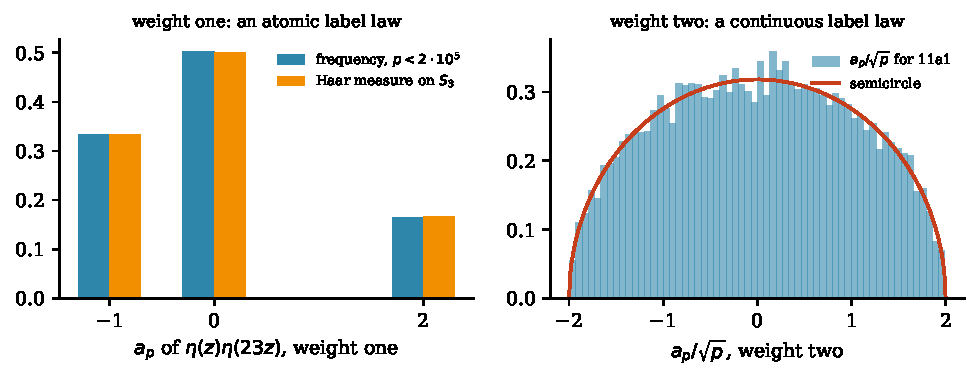
\includegraphics[width=\textwidth]{figs/flt_labels.pdf}
\caption{Proposition~\ref{prop:fltatomic}. Left: the coefficients of the weight one form $\eta(z)\eta(23z)$ over primes below $2\cdot10^5$, against Haar measure on $S_3$. Right: the normalised coefficients of the weight two form of $11a1$, against the semicircle.}\label{fig:fltlabels}
\end{figure}

\section{Modularity and symmetry in law}\label{sec:fltsymmetry}

Let $E$ have conductor $N$ and $L$ series $\sum a_nn^{-s}$, and put $f(z)=\sum a_ne^{2\pi inz}$. The P\'olya kernel of Chapter~\ref{ch:recip},
\[
\Phi_E(u)=f\Bigl(\frac{ie^u}{\sqrt N}\Bigr)e^{u},\qquad \Lambda(1+t,E)=\int_{\R}\Phi_E(u)e^{tu}\,du,
\]
with $\Lambda(s,E)=N^{s/2}(2\pi)^{-s}\Gamma(s)L(s,E)$, is built from the point counts $a_p=p+1-|E(\mathbb F_p)|$ and the conductor. By Hecke's criterion (Proposition~\ref{prop:recipsym}), $f$ satisfies the Fricke transformation with root number $\varepsilon$ if and only if $\Phi_E(-u)=\varepsilon\,\Phi_E(u)$. Weil's converse theorem \cite{weil1967} upgrades the corresponding reflection identities for the twisted kernels $\Phi_{E\otimes\chi}$, which pair $\chi$ with $\bar\chi$ and are complex valued, to modularity; Problem~\ref{cp:recipkernel} poses their numerical test. For $11a1$ the reflection of $\Phi_E$ alone suffices, given the Euler product: the converse theorem of Conrey and Farmer \cite{conreyfarmer1995} replaces the twists by the shape of the Euler factors at the levels $5\le N\le12$, $14\le N\le17$ and $23$. So Theorem~\ref{thm:fltwiles} says, for a semistable $E$, that a family of functions built from point counts and the conductor has the reflection symmetries of a modular form.

\begin{proposition}[the P\'olya variable of an elliptic curve; after Proposition~\ref{prop:recipsym}]\label{prop:fltsymmetric}
Let $f$ be the newform of an elliptic curve $E$ and suppose $\Phi_E\ge0$. Then $\Phi_E/\Lambda(1,E)$ is the density of a random variable $W_E$ with $\E e^{tW_E}=\Lambda(1+t,E)/\Lambda(1,E)$ for all real $t$, and $W_E$ is symmetric in law; positivity forces the root number to be $+1$, since a kernel with $\varepsilon=-1$ is odd. For $E=11a1$, $f(z)=\eta(z)^2\eta(11z)^2$ is positive on the imaginary axis, so $W_E$ exists and is symmetric.
\end{proposition}

\begin{proof}
The Mellin formula gives the transform, which converges for all real $t$ because $f(iy)$ decays exponentially as $y\to\infty$ and, by the Fricke symmetry, as $y\to0$. Symmetry is Hecke's criterion with $\varepsilon=+1$. The product formula $\eta(z)=q^{1/24}\prod(1-q^n)$ is positive on $z=iy$, and the root number of $11a1$ is $+1$.
\end{proof}

We computed $\Phi_E$ from the first $4000$ coefficients for $11a1$ and $37a1$ (Figure~\ref{fig:fltkernels}, left). For $11a1$ the kernel is positive, with minimum $1.2\cdot10^{-9}$ on $|u|\le2.5$, and $\max|\Phi_E(u)-\Phi_E(-u)|=9\cdot10^{-17}$. For $37a1$, the curve of smallest conductor with positive rank, the root number is $-1$ and the kernel is odd to $4\cdot10^{-16}$: the parity of the analytic rank is the parity of a P\'olya kernel. A Frey curve, if it existed, would by Theorem~\ref{thm:fltwiles} have kernels with all the twisted reflection symmetries; by Ribet its mod $p$ labels would agree with those of a level $2$ form; there is none.

\begin{figure}[t]
\centering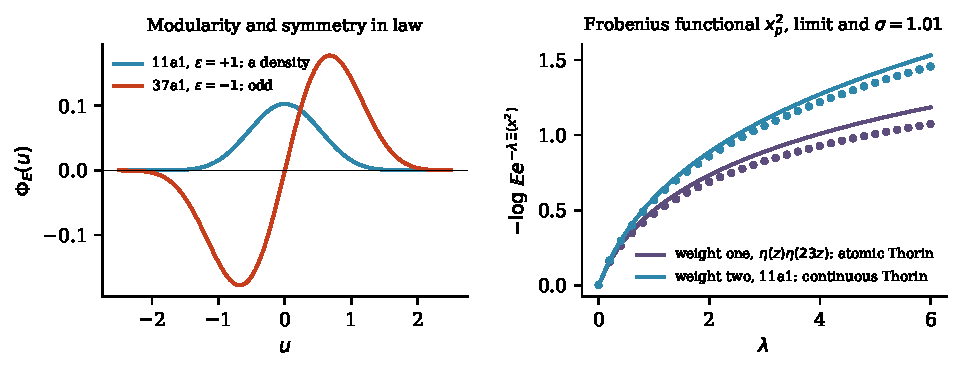
\includegraphics[width=\textwidth]{figs/flt_kernels.pdf}
\caption{Left: P\'olya kernels $\Phi_E(u)$ (solid) and $\varepsilon\Phi_E(-u)$ (dashed, hidden under the solid curves) computed from point counts and the conductor: $11a1$, a positive multiple of a symmetric probability density, and $37a1$, odd. Right: the Frobenius functional $\Xi_\sigma(Q)$, $Q(x)=x^2$, of the zeta random integer for the weight one form $\eta(z)\eta(23z)$ and the weight two form of $11a1$, shown as $-\log\E e^{-\lambda\,\Xi_\sigma(Q)}$: the limits $\int\log(1+\lambda x^2)\,d\mu$ (lines) and the values at $\sigma=1.01$ from the Euler product over the primes below $10^7$, the rest estimated by the prime number theorem (dots). Both have mean $1$; their Thorin measures differ.}\label{fig:fltkernels}
\end{figure}

\section{The Thorin measures of an elliptic curve}\label{sec:fltthorinec}

For an elliptic curve, or any weight two newform, there are three Thorin objects, of increasing depth.

\emph{Frobenius functionals.} By Theorem~\ref{thm:recipggcfun} the functional $\Xi_\sigma(Q)$ of the zeta random integer, with labels $x_p=a_p/\sqrt p$, converges to the GGC whose Thorin measure is the image of the label law, restricted to $\{Q>0\}$, under $x\mapsto1/Q(x)$. For $Q(x)=x^2$ and $11a1$ this is the law of $1/X^2$ for $X$ semicircular, a continuous Thorin measure; for the weight one form $\eta(z)\eta(23z)$ it is atomic, $\frac16\delta_{1/4}+\frac13\delta_1$. Both GGCs have mean $\int x^2\,d\mu=1$, which is the orthonormality of Theorem~\ref{thm:recipcusp} in the form \emph{unit second moment}; the Thorin measures, images of the label laws, are what distinguish weight one from weight two (Figure~\ref{fig:fltkernels}, right; Proposition~\ref{prop:fltatomic}). These statements are unconditional.

\emph{The Rankin Selberg GGC.} Let $D(s)$ be the Rankin Selberg Euler product of $E$ in the unitary normalisation, with $\alpha_p=a_p/\sqrt p$ and $\beta_p=0$ at the primes $p\mid N$, so that $-D'/D(s)=\sum_{p,m}|\alpha_p^m+\beta_p^m|^2(\log p)p^{-ms}$ with nonnegative coefficients and $D$ has a pole at $s=1$; for semistable $E$, $D$ is $L(s,E\times E)$ without its factors $(1-p^{-s})^{-1}$ at the primes $p\mid N$. For $\alpha>1$ put
\[
U_\alpha(z)=\frac1{2\pi\sqrt z}\sum_{p,m}|\alpha_p^m+\beta_p^m|^2(\log p)\,p^{-m\alpha}\,2\sin^2\Bigl(\frac{m\log p\,\sqrt z}2\Bigr).
\]
By Lemma~\ref{lem:10dsin2} with $f=D$, as for the density $U_{\mathrm{ar}}$ of Section~\ref{sec:10daway} (Proposition~\ref{prop:recipfamily} is the analogue for Artin representations),
\[
e^{\sqrt s\,D'/D(\alpha)}\,\frac{D(\alpha)}{D(\alpha+\sqrt s)}
\]
is the Laplace transform of a GGC with Thorin density $U_\alpha$. It is computed from point counts and is positive unconditionally. Figure~\ref{fig:fltthorinec}, right, shows $U_\alpha$ for $11a1$ at $\alpha=1.5$ and $1.2$, with the bad prime $11$ entering through $|\alpha_{11}^m|^2=11^{-m}$; it grows as $\alpha$ decreases towards the pole at $s=1$.

\emph{The zeros.} The deepest object is the Galois heat trace $\mathcal W_E$ of Definition~\ref{def:recipheat}, given by the explicit formula from the point counts, the conductor and the gamma factor. Since $L(s,E)$ is entire by modularity (Theorem~\ref{thm:02modularity}), Theorem~\ref{thm:recipcm} gives $\mathcal W_E(x)=\frac12\sum e^{-x\gamma^2}$, the sum over the zeros $1+i\gamma$ of $\Lambda(s,E)$ with multiplicity, which are the zeros $\frac12+i\gamma$ in the unitary normalisation of Chapter~\ref{ch:recip}, and $\mathcal W_E$ is completely monotone if and only if GRH holds for $L(s,E)$. Its Bernstein measure is then $\frac r2\delta_0+\sum_{\gamma>0}\delta_{\gamma^2}$, where $r$ is the order of the zero at the centre, which is odd when the root number is $-1$; for $11a1$, $r=0$. If $r=0$ and GRH holds, Theorem~\ref{thm:hitexplosion} makes $\mathcal W_E(x)/x$ the L\'evy density of the explosion time $T_E$ of a pure birth process with rates $\gamma^2$, with $\E T_E=\int_0^\infty\mathcal W_E(x)\,dx=\sum_{\gamma>0}\gamma^{-2}$; by the same theorem $T_E$ exists only if GRH holds for $L(s,E)$, which is not known.

For $11a1$ we computed $\mathcal W_E$, as Chapter~\ref{ch:hit} does for the $S_3$ representation, from the conductor $11$, the gamma factor and the point counts at the $664579$ primes below $10^7$ and their powers, with the bad prime $11$ entering through $a_{11}=1$. It agrees with the sum over the zeros to fifteen digits at $x=0.002$, $0.01$ and $0.05$ and to thirteen digits at $x=0.2$ (Figure~\ref{fig:fltthorinec}, left), finite differences give its first two derivatives the signs required by complete monotonicity at $x=0.05,0.1,0.2,0.4$, and
\[
\int_{e^{-60}}^{2}\mathcal W_E(x)\,dx=0.127589010327
\]
from point counts, against $0.127589010329$ computed by PARI for $\frac12\sum\gamma^{-2}=\frac12\Lambda''(1,E)/\Lambda(1,E)$, an identity of the Hadamard product that needs no hypothesis; this is the constant $S_1$ of $11a1$ in Table~\ref{tab:10bcatalogue}. The first zero is $\gamma_1=6.3626$, so $\mathcal W_E(x)<e^{-80}$ for $x\ge2$, and the difference $1.6\cdot10^{-12}$ is the part of the integral over $x<e^{-60}$, which the quadrature leaves out and which the density of the zeros gives as $1.55\cdot10^{-12}$; with it the two values differ by $6\cdot10^{-17}$. As in Chapter~\ref{ch:hit}, the agreement does not verify GRH: a finite computation of this kind can disprove it and is not known to verify it.

\begin{proposition}[an explicit Wald couple; after Theorem~\ref{thm:10dvdp}]\label{prop:fltwald}
Assume GRH for $L(s,11a1)$. Then the P\'olya variable $W_E$ of Proposition~\ref{prop:fltsymmetric} and the explosion time $T_E$ satisfy\[\E e^{tW_E}\,\E e^{-t^2T_E}=1\qquad\text{for every real }t:\]they form a Wald couple in the sense of Definition~\ref{def:10dwald}, built respectively from the modular form $\eta(z)^2\eta(11z)^2$ and from the zeros of its $L$ function.
\end{proposition}

\begin{proof}
This is the implication from (a) to (c) of Theorem~\ref{thm:10dvdp} for $\eta(z)^2\eta(11z)^2$, with $Z_\pi=T_E$. Directly: $\E e^{tW_E}=\Lambda(1+t,E)/\Lambda(1,E)$, and under GRH
\[
\E e^{-t^2T_E}=\prod_{\gamma>0}\Bigl(1+\frac{t^2}{\gamma^2}\Bigr)^{-1}=\frac{\Lambda(1,E)}{\Lambda(1+t,E)}
\]
by the Hadamard product, since $\Lambda(1,E)\ne0$ and $\Lambda(1+z,E)$ is even of order one, so its exponential factors cancel in pairs.
\end{proof}

\begin{figure}[t]
\centering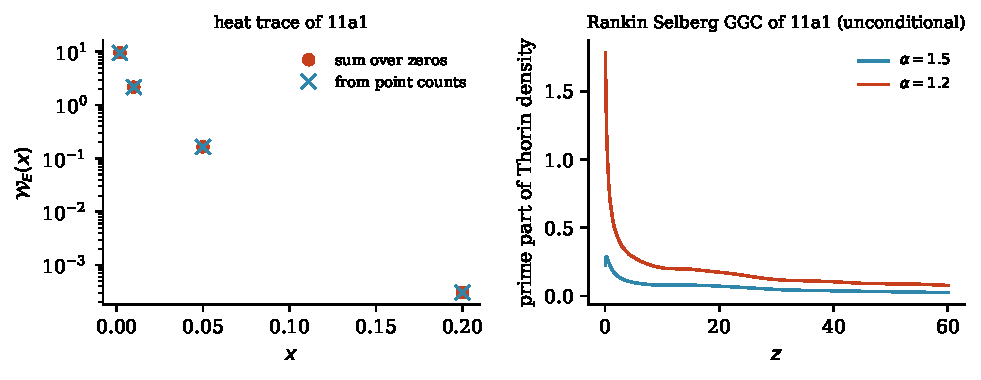
\includegraphics[width=\textwidth]{figs/flt_thorin.pdf}
\caption{Left: the heat trace of $11a1$ computed from the point counts modulo the primes below $10^7$, the conductor and the gamma factor (crosses), against the sum over its zeros (dots). Right: the Rankin Selberg Thorin density $U_\alpha$ of $11a1$ at $\alpha=1.5$ and $1.2$, positive unconditionally, summed over the primes below $10^7$; the larger primes would add under $0.4$ percent at $\alpha=1.5$ and between $3.5$ and $9.3$ percent at $\alpha=1.2$.}\label{fig:fltthorinec}
\end{figure}

\section{Weight two forms are one forms}\label{sec:fltoneforms}

For $f\in S_2(\Gamma_0(N))$ the differential $f(z)\,dz$ is invariant under $\Gamma_0(N)$ and holomorphic at the cusps, and every holomorphic $1$ form on $X_0(N)$ arises this way, so $\dim S_2(\Gamma_0(N))=g(X_0(N))$. For prime $N$, by Deuring \cite{deuring1941} and Eichler, the number of supersingular elliptic curves over $\overline{\mathbb F}_N$ is $g(X_0(N))+1$, and by Eichler and Gross the $1$ forms on $X_0(N)$ correspond to the nonconstant eigenfunctions of the isogeny walk of Section~\ref{sec:hitisogeny} \cite{eichler1954,eichler1973,gross1987} (Theorem~\ref{thm:08brandt} for $N\equiv1\bmod12$). The genus is zero exactly for $N\in\{2,3,5,7,13\}$ among primes; PARI/GP gives $\dim S_2(\Gamma_0(N))=0,0,0,0,1,0,1,1,2$ for $N=2,3,5,7,11,13,17,19,23$.

At $N=2$ there is one supersingular curve, $j=0=1728$ in characteristic $2$, with automorphism group of order $24$; with $w=|\operatorname{Aut}E|/2=12$, Eichler's mass formula $\sum1/w=(N-1)/12$ of Chapter~\ref{ch:hit} reads $1/12=1/12$. Its endomorphism ring is the Hurwitz order of quaternions $\frac12(a+bi+cj+dk)$ with $a,b,c,d$ all even or all odd, which has class number one. The theta series of its norm form lies in $M_2(\Gamma_0(2))$, which is spanned by an Eisenstein series because $S_2(\Gamma_0(2))=0$, and so counts exactly: the number of Hurwitz quaternions of norm $n$ is $24\sum_{d\mid n,\,d\text{ odd}}d$. We checked this by enumeration for $n\le60$; the first values are $24,24,96,24,144,96,192,24$. The isogeny walk has a single state, and every $\ell$ isogeny returns to the same curve.

\section{Is there a Thorin measure form of Fermat's last theorem?}\label{sec:fltthorin}

The answer has three parts.

First, no Thorin statement is \emph{equivalent} to Fermat's last theorem in a useful sense. Fermat is about rational points on the curves $x^p+y^p=1$; Thorin measures are attached to $L$ functions and Frobenius statistics. The bridge used in the proof, and the only one known for all exponents, is modularity, a deep theorem. Any true statement is formally equivalent to any other, so the question is what Fermat \emph{reduces to}, after the deep theorems.

Second, it reduces to the emptiness of a Thorin measure.

\begin{definition}\label{def:flthecke}
For a prime $N$ and a prime $\ell\ne N$, the \emph{Hecke GGC} $H_N(\ell)$ is the generalized gamma convolution with Thorin measure $\sum_f\delta_{\ell+1-a_\ell(f)}$, the sum over the normalised eigenforms of $S_2(\Gamma_0(N))$.
\end{definition}

The atoms are positive because $a_\ell(f)<\ell+1$, which Perron Frobenius gives on the connected supersingular isogeny graph (the bound $|a_\ell(f)|\le2\sqrt\ell$ of Eichler and Shimura with Weil, as in Chapter~\ref{ch:hit}, gives more), so $H_N(\ell)$ is a sum of independent exponential variables with rates $\ell+1-a_\ell(f)$, the time that a pure birth chain with these rates takes to pass through its states. For a rational $f$ attached to an elliptic curve $E_f$ the rate is $|E_f(\mathbb F_\ell)|$. By \eqref{eq:hitjac} and Theorem~\ref{thm:hitkemeny},
\[
\E e^{-sH_N(\ell)}=\prod_f\frac{\ell+1-a_\ell(f)}{\ell+1+s-a_\ell(f)}=\frac{|J_0(N)(\mathbb F_\ell)|}{\det\bigl((\ell+1+s)-T_\ell\mid S_2(\Gamma_0(N))\bigr)},
\]
and $\E H_N(\ell)=K_N(\ell)/(\ell+1)$, with $K_N(\ell)$ the Kemeny constant of the supersingular $\ell$ isogeny walk in characteristic $N$. Chapter~\ref{ch:lap} inverts this transform through the B spline whose knots are the atoms $\ell+1-a_\ell(f)$ (Theorem~\ref{thm:lapspline}).

\begin{theorem}[empty Thorin measures]\label{thm:fltempty}
For a prime $N$ and a prime $\ell\ge5$, $\ell\ne N$, the following are equivalent.
\begin{enumerate}
\item[(a)] The curve $X_0(N)$ has genus zero, so it carries no nonzero holomorphic $1$ form and $S_2(\Gamma_0(N))=0$.
\item[(b)] The Thorin measure of $H_N(\ell)$ is zero, that is $H_N(\ell)=0$ almost surely.
\item[(c)] $|J_0(N)(\mathbb F_\ell)|=1$.
\item[(d)] There is exactly one supersingular elliptic curve over $\overline{\mathbb F}_N$, and the isogeny walk has a single state.
\item[(e)] The Kemeny constant $K_N(\ell)$ vanishes.
\end{enumerate}
\end{theorem}

\begin{proof}
(a) and (b) are the same statement, since the atoms are indexed by eigenforms. (a) implies (c) because $J_0(N)=0$. If $g\ge1$, the Weil bound gives $|J_0(N)(\mathbb F_\ell)|=\prod_f(\ell+1-a_\ell(f))\ge(\sqrt\ell-1)^{2g}$, as in Corollary~\ref{cor:hithasse}, and $(\sqrt5-1)^2>1$, so (c) implies (a). (a) is equivalent to (d) by the count $g+1$ of supersingular curves, and to (e) by Theorem~\ref{thm:hitkemeny}, which writes $K_N(\ell)$ as a sum of $g$ positive terms.
\end{proof}

Third, Ribet's theorem produces a newform whose mod $p$ discrepancy Thorin mass against the given one vanishes; equivalently, by Theorem~\ref{thm:hitrate}, the discrepancy set of primes is hit by the prime factors of a random integer at rate zero. Label the primes by the pair of mod $p$ Frobenius classes of two Galois representations; by Chebotarev these labels are equidistributed on a finite group, and Theorem~\ref{thm:recipggcfun} applies with a finite label space, as in Theorem~\ref{thm:recipthorin}(a) for Artin representations.

\begin{proposition}[mod $p$ reciprocity as a vanishing Thorin mass; compare Theorem~\ref{thm:recipthorin}(a)]\label{prop:fltmodp}
Let $\rho_1,\rho_2$ be the representations, at primes above $p$ of the coefficient fields, of two weight two newforms with trivial character, or of an elliptic curve and such a newform, with semisimple reductions $\bar\rho_1,\bar\rho_2$ over a common finite field $k$ of characteristic $p$. Let $D_p$ be the set of primes $\ell\nmid pN_1N_2$ with $\tr\bar\rho_1(\Frob_\ell)\ne\tr\bar\rho_2(\Frob_\ell)$ in $k$, and $Q=\mathsf 1_{D_p}$. The following are equivalent: (i) $\bar\rho_1\cong\bar\rho_2$; (ii) $D_p$ has Dirichlet density zero; (iii) the Frobenius functional $\Xi_\sigma(Q)$ of the zeta random integer converges to $0$, its Thorin measure being zero.
\end{proposition}

\begin{proof}
Both representations factor through the finite group $G=\Gal(K/\Q)$ cut out by $\bar\rho_1\oplus\bar\rho_2$, and $D_p$ is the set of primes whose Frobenius lies in the union of classes where $\tr\bar\rho_1\ne\tr\bar\rho_2$. By Chebotarev its density is the Haar measure of that union, which is also the Thorin mass of the limit of $\Xi_\sigma(Q)$ by Theorem~\ref{thm:recipggcfun}. If the density is zero the traces agree on all of $G$; both determinants are the mod $p$ cyclotomic character, so the characteristic polynomials agree, and the Brauer Nesbitt theorem gives (i). The converse is clear.
\end{proof}

Figure~\ref{fig:fltcongruence} illustrates Proposition~\ref{prop:fltmodp} with a congruence between levels. The curve $11a1$ has $a_7=-2\equiv-(7+1)\bmod3$, which is Ribet's condition \cite{ribet1984} for level raising at $q=7$ modulo $3$, and indeed one of the three rational newforms of level $77$ agrees with $11a1$ modulo $3$ at all $2259$ primes $\ell<2\cdot10^4$ prime to $3\cdot7\cdot11$, consistent with zero discrepancy Thorin mass; Ribet's level raising theorem predicts a newform of level $77$ congruent to $11a1$ modulo a prime above $3$, and here it has rational coefficients. The other two disagree at $57$ and $66$ percent of these primes. Read from level $77$ down to level $11$, this is level lowering at $q=7$, the step that Ribet's theorem performs for the Frey curve.

\begin{figure}[t]
\centering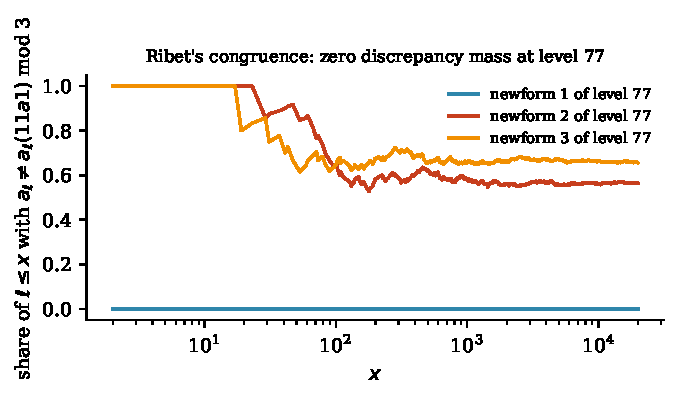
\includegraphics[width=0.72\textwidth]{figs/flt_congruence.pdf}
\caption{Proposition~\ref{prop:fltmodp}: the share of primes $\ell\le x$ at which the coefficients of each rational newform of level $77$ differ modulo $3$ from those of $11a1$. One newform has no discrepancy prime below $2\cdot10^4$, consistent with Ribet's level raising theorem \cite{ribet1984}, which predicts from the condition $a_7(11a1)\equiv-(7+1)\bmod3$ a newform of level $77$ congruent to $11a1$ modulo a prime above $3$.}\label{fig:fltcongruence}
\end{figure}

\begin{theorem}[Fermat's last theorem in Thorin form]\label{thm:fltflt}
Assume Theorems~\ref{thm:fltwiles} and \ref{thm:fltribet} and Mazur's torsion theorem \cite{mazur1977}. Then for every prime $p\ge5$ a solution of $a^p+b^p=c^p$ in nonzero integers would produce a weight two newform $g$ of level dividing $2$ whose mod $p$ discrepancy Thorin mass against the Frey curve is zero. Since $S_2(\Gamma_0(1))=0$ and the Thorin measure of $H_2(\ell)$ is empty (Theorem~\ref{thm:fltempty}), no such $g$ exists, and Fermat's last theorem holds for $p\ge5$.
\end{theorem}

\begin{proof}
The Frey curve $E$ is semistable, hence modular by Theorem~\ref{thm:fltwiles}, with $\bar\rho_{E,p}$ irreducible by Serre's argument from Mazur's torsion theorem \cite{serre1987} (see Proposition~\ref{prop:flteisfrey}), unramified at every odd prime dividing $N_E$ other than $p$, and finite flat at $p$. Apply Theorem~\ref{thm:fltribet} first at $q=p$ if $p\mid N_E$, where $q\not\equiv1\bmod p$ holds trivially, and then one at a time at the odd primes $q\ne p$ of the level, which is now prime to $p$. This gives a newform $g$ of level dividing $2$ and a prime $\mathfrak p'$ above $p$ with $\bar\rho_{g,\mathfrak p'}\cong\bar\rho_{E,p}$ over $\overline{\mathbb F}_p$, which by Proposition~\ref{prop:fltmodp} is the vanishing of the discrepancy Thorin mass. But $S_2(\Gamma_0(1))=0$, and $X_0(2)$ has genus zero, so by Theorem~\ref{thm:fltempty} there are no weight two newforms of level $2$.
\end{proof}

With the exponents $3$ (Euler) and $4$ (Fermat) this gives every $n\ge3$, since each is divisible by $4$ or by an odd prime. So the last line of the proof of Fermat's last theorem, $S_2(\Gamma_0(2))=0$, is elementary, and in the language of this chapter it reads: in characteristic $2$ there is one supersingular elliptic curve, so the isogeny walk is stuck, its Kemeny constant is zero, the Hecke GGC is the zero variable, and its Thorin measure is empty. Equivalently, the Hurwitz quaternions have class number one. Everything before that line is the work of Hellegouarch and Frey (the curve), Frey and Serre (the reduction), Mazur, Ribet, Langlands and Tunnell, Wiles, and Taylor and Wiles (Sections~\ref{sec:fltproof} and \ref{sec:fltweightone}).

\section{Fermat's last theorem, one Thorin measure at a time}\label{sec:fltexplicit}

The previous section answered the title question in outline. This section makes every Thorin measure in the argument explicit: on which space it lives, what it is, which theorem says that it vanishes or does not, and what it is numerically. Two Thorin measures appear. The first, the \emph{Eisenstein Thorin shape} of an elliptic curve, is a single number $c(E,p)\in[0,1]$: the density of the primes $\ell$ with $p\nmid|E(\mathbb F_\ell)|$, which is the local density at $p$ in Koblitz's conjecture \cite{koblitz1988}, in Zywina's form for any image \cite{zywina2011}, read here as the shape of a Gamma law. Mazur's torsion theorem, through Serre's argument, makes it positive for Frey curves when $p\ge5$. The second is the Hecke Thorin measure of Definition~\ref{def:flthecke}, which is empty at level $2$. Given Theorems~\ref{thm:fltwiles} and \ref{thm:fltribet} and Mazur's torsion theorem, a Frey curve, whose shape is positive, would give the second measure an atom; since it has none, there is no Frey curve (Theorem~\ref{thm:flttwo}).

\subsection{The Eisenstein Thorin shape}

The weight two Eisenstein series of prime level $N$ has Hecke eigenvalues $a_\ell=1+\ell$ for $\ell\ne N$. For an elliptic curve the difference from Eisenstein is a point count: $1+\ell-a_\ell(E)=|E(\mathbb F_\ell)|$. So ``$E$ agrees with Eisenstein modulo $p$ at $\ell$'' means exactly that $p$ divides $|E(\mathbb F_\ell)|$.

\begin{definition}\label{def:flteis}
Let $E/\Q$ have conductor $N$ and let $p$ be prime. The \emph{Eisenstein discrepancy} of $(E,p)$ is $Q_{E,p}(\ell)=\mathsf 1\{p\nmid|E(\mathbb F_\ell)|\}$ for primes $\ell\nmid pN$, and its \emph{Eisenstein Thorin shape} is
\[
c(E,p)=\mu_{G_{E,p}}\bigl\{g\in G_{E,p}:\det(1-g)\ne0\bigr\},
\]
where $G_{E,p}\subset\GL_2(\mathbb F_p)$ is the image of $\bar\rho_{E,p}$, with Haar probability measure $\mu_{G_{E,p}}$.
\end{definition}

\begin{proposition}[Gamma law of the Eisenstein discrepancy; (a) this book]\label{prop:flteisgamma}
Let $E/\Q$ be an elliptic curve and $p$ a prime.
\begin{enumerate}
\item[(a)] The Frobenius functional $\Xi_\sigma(Q_{E,p})$ of the zeta random integer converges in law, as $\sigma\downarrow1$, to the Gamma law with shape $c(E,p)$ and scale $1$. Its Thorin measure is $c(E,p)\,\delta_1$, and $c(E,p)$ is the rate at which the prime factors of a random integer hit the primes $\ell$ with $p\nmid|E(\mathbb F_\ell)|$ (Theorem~\ref{thm:hitrate}).
\item[(b)] $c(E,p)=0$ if and only if $\bar\rho_{E,p}^{\mathrm{ss}}\cong1\oplus\chi_p$, with $\chi_p$ the mod $p$ cyclotomic character, if and only if $p$ divides $|E(\mathbb F_\ell)|$ for every $\ell\nmid pN$. In that case $E$ has a rational isogeny of degree $p$. If $E$ is semistable, $c(E,p)=0$ if and only if $\bar\rho_{E,p}$ is reducible.
\item[(c)] If $G_{E,p}=\GL_2(\mathbb F_p)$, then
\[
c(E,p)=c_p:=1-\frac{p^2-2}{(p^2-1)(p-1)},
\]
so that $c_2=\frac13$, $c_3=\frac9{16}$, $c_5=\frac{73}{96}$ and $c_7=\frac{241}{288}$.
\end{enumerate}
\end{proposition}

\begin{proof}
(a) The label of $\ell$ is the conjugacy class of $\bar\rho_{E,p}(\Frob_\ell)$ in the finite group $G_{E,p}$, and $Q_{E,p}(\ell)=1$ exactly when $\det\bigl(1-\bar\rho_{E,p}(\Frob_\ell)\bigr)$, which is $|E(\mathbb F_\ell)|$ modulo $p$, is nonzero. By Chebotarev the labels are equidistributed for Haar measure, and Theorem~\ref{thm:recipggcfun} with $Q\in\{0,1\}$ gives the GGC whose Thorin measure is $\mu(Q=1)\,\delta_1=c(E,p)\,\delta_1$, the Gamma law with shape $c(E,p)$. The hitting rate is Theorem~\ref{thm:hitrate} for the same set of primes.

(b) If $c(E,p)=0$ then every $g\in G_{E,p}$ has eigenvalue $1$, so its characteristic polynomial is $(x-1)(x-\det g)$, which is that of $1\oplus\chi_p$ since $\det\bar\rho_{E,p}=\chi_p$. By Brauer Nesbitt $\bar\rho_{E,p}^{\mathrm{ss}}\cong1\oplus\chi_p$, so $\bar\rho_{E,p}$ is reducible and its invariant line gives a rational $p$ isogeny. The converse and the point count form are immediate. For semistable $E$ the two characters of a reducible $\bar\rho_{E,p}$ are $1$ and $\chi_p$ \cite{serre1972}, so reducibility forces $c(E,p)=0$.

(c) In $\GL_2(\mathbb F_p)$ the elements with eigenvalue $1$ have characteristic polynomial $(x-1)(x-d)$. For each of the $p-2$ values $d\ne0,1$ these form one split semisimple class of size $p(p+1)$; for $d=1$ there are the identity and the $p^2-1$ nontrivial unipotents. The count is $(p-2)p(p+1)+p^2=p^3-2p$, and dividing by $|\GL_2(\mathbb F_p)|=(p^2-1)(p^2-p)$ gives $(p^2-2)/((p^2-1)(p-1))$.
\end{proof}

Part (c) is the class count behind the factor at $p$ of the constant in Koblitz's conjecture on the primality of $|E(\mathbb F_\ell)|$ \cite{koblitz1988,zywina2011}: $c_p/(1-1/p)=1-(p^2-p-1)/((p-1)^3(p+1))$. By a theorem of Katz \cite{katz1981}, the curves with $c(E,p)=0$ in (b) are those isogenous to a curve with a rational point of order $p$. What (a) adds is the reading of this density as the shape of a Gamma law.

So the Eisenstein shape is a Thorin measure with one atom, and the whole content is in the mass of that atom. Two of its behaviours appear in the book's running examples (Figure~\ref{fig:flteis}). For $11a1$ and $p=5$ the shape is exactly $0$: $11a1$ has a rational point of order $5$, so $5$ divides $|11a1(\mathbb F_\ell)|$ for all $664577$ primes $\ell<10^7$ with $\ell\ne5,11$, and the Laplace transform of $\Xi_\sigma(Q)$ is identically $1$. This is Mazur's Eisenstein congruence \cite{mazur1977}: $J_0(11)$ is the curve $11a1$, whose rational torsion, the cuspidal subgroup, has order $5$, the numerator of $(11-1)/12$, and injects into $J_0(11)(\mathbb F_\ell)$ for $\ell\ne11$ (for $\ell\ge3$ by the appendix of \cite{katz1981}, and for $\ell=2$ because its order is odd), so $5$ divides the product $|J_0(11)(\mathbb F_\ell)|$ of the Thorin atoms of $H_{11}(\ell)$. For $37a1$, whose mod $p$ images are all of $\GL_2(\mathbb F_p)$ \cite{serre1972}, the observed shares of discrepancy primes below $10^7$ are $0.3332$, $0.5628$, $0.7611$, $0.8370$, $0.9002$, $0.9178$ for $p=2,3,5,7,11,13$, against $c_p=0.3333$, $0.5625$, $0.7604$, $0.8368$, $0.9008$, $0.9172$, and the Laplace transforms at $\sigma=1.01$ and $\sigma=1.002$ approach $(1+\lambda)^{-c_p}$.

\begin{figure}[t]
\centering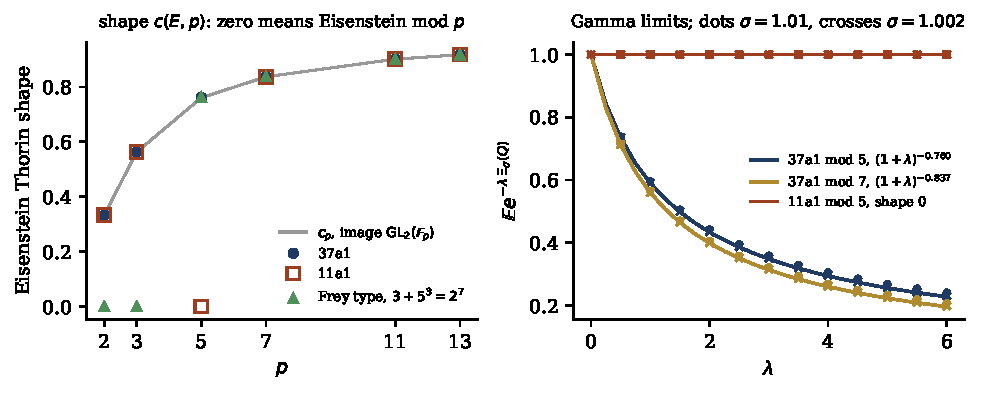
\includegraphics[width=\textwidth]{figs/flt_eisenstein.pdf}
\caption{Proposition~\ref{prop:flteisgamma}. Left: the Eisenstein Thorin shape $c(E,p)$, measured as the share of primes $\ell<10^7$ with $p\nmid|E(\mathbb F_\ell)|$ for $37a1$ and $11a1$, and of primes $\ell<2\cdot10^6$ for the semistable Frey type curve $y^2=x(x+125)(x+128)$ of $3+5^3=2^7$, against $c_p$. Right: Laplace transforms of $\Xi_\sigma(Q_{E,p})$ for $37a1$ modulo $5$ and $7$ and $11a1$ modulo $5$, at $\sigma=1.01$ (dots) and $\sigma=1.002$ (crosses), against the Gamma limits $(1+\lambda)^{-c(E,p)}$.}\label{fig:flteis}
\end{figure}

\subsection{Mazur's theorem and the Eisenstein shape of a Frey curve}

A Frey curve $y^2=x(x-a^p)(x+b^p)$ is semistable and has all its $2$ torsion rational. The second fact gives the Eisenstein shape $c(E,2)=0$, and with Mazur's torsion theorem it gives positive shapes at every $p\ge5$.

\begin{proposition}[Eisenstein shapes of a Frey curve; after Serre \cite{serre1987} and Mazur \cite{mazur1977}]\label{prop:flteisfrey}
Let $E$ be an elliptic curve over $\Q$ with $E[2]\subset E(\Q)$, for example a Frey curve. Then $c(E,2)=0$, and $c(E,p)>0$ for every prime $p\ge5$.
\end{proposition}

\begin{proof}
For odd $\ell$ of good reduction, reduction is injective on $E(\Q)[2]\cong(\Z/2)^2$, so $4$ divides $|E(\mathbb F_\ell)|$ and $Q_{E,2}\equiv0$. If $c(E,p)=0$ for some $p\ge5$, then $\bar\rho_{E,p}^{\mathrm{ss}}\cong1\oplus\chi_p$ by Proposition~\ref{prop:flteisgamma}(b), so $E$, or its quotient $E'$ by the rational subgroup of order $p$, has a rational point of order $p$. An isogeny of odd degree maps $E[2]$ isomorphically onto $E'[2]$, so that curve has rational torsion containing $\Z/2\times\Z/2p$, which Mazur's torsion theorem \cite{mazur1977} excludes for $p\ge5$. This is Serre's argument \cite{serre1987}; see also \cite[Theorem~2.9(c)]{ddt1995}.
\end{proof}

So the irreducibility of $\bar\rho_{E,p}$ for a Frey curve and $p\ge5$, the hypothesis of Ribet's theorem that Serre deduced from Mazur's torsion theorem, reads in Thorin form: the Gamma law of the Eisenstein discrepancy has positive shape; equivalently, $p$ fails to divide $|E(\mathbb F_\ell)|$ for a positive proportion $c(E,p)$ of primes. The hypothesis $p\ge5$ is sharp, and a real Frey type curve shows why. The $abc$ triple $3+5^3=2^7$, written as $-125+128=3$ with $-125\equiv-1\bmod4$ and $32\mid128$, gives the Frey type curve
\[
E_0:\ y^2=x(x+125)(x+128),
\]
which is semistable of conductor $30$ with minimal discriminant $2^63^25^6$. Its shapes, measured over the primes below $2\cdot10^6$, are $c(E_0,2)=0$ and $c(E_0,3)=0$, but $c(E_0,5)=0.762$ and $c(E_0,7)=0.837$, against $c_5=0.760$ and $c_7=0.837$ (Figure~\ref{fig:flteis}, left). At $p=3$ the exponents $6$ and $6$ of the primes $2$ and $5$ are divisible by $3$, so $\bar\rho_{E_0,3}$ is unramified at $2$ and $5$. A genuine Frey curve differs at $2$: there the exponent is $2pv_2(b)-8$, never divisible by an odd $p$, which is why level $2$ remains. And $E_0$ has a rational $3$ isogeny, its Eisenstein shape at $3$ is $0$, and Ribet's theorem, which needs an irreducible $\bar\rho$, does not apply. At $p\ge5$, where Mazur's torsion theorem forces the shape to be positive, the exponents are not divisible by $p$ and there is nothing to lower. A genuine Frey curve would need both at once.

\subsection{The level two Brandt module}

At level $N=2$ the isogeny walk has the single state of Section~\ref{sec:fltoneforms}, and its Brandt matrix is the $1\times1$ matrix $B(\ell)=(\ell+1)$. By Eichler and Gross \cite{eichler1954,eichler1973,gross1987} the constants carry the Eisenstein eigenvalues $\ell+1$, and their orthogonal complement in $L^2$ of the stationary law carries $S_2(\Gamma_0(2))$, which is $0$ here. So every weight two Hecke eigensystem of level $2$, cuspidal or not, is visible on this one point space, and a mod $p$ eigensystem there could be of two kinds, of which only the first occurs:
\begin{enumerate}
\item[(E)] the Eisenstein system $a_\ell=\ell+1$ of the stationary law, against which a curve $E$ has discrepancy Thorin shape $c(E,p)$;
\item[(C)] a cuspidal system, an atom of the Hecke Thorin measure of $H_2(\ell)$, which is empty by Theorem~\ref{thm:fltempty}.
\end{enumerate}

\begin{theorem}[Fermat's last theorem as two Thorin statements]\label{thm:flttwo}
Assume Theorems~\ref{thm:fltwiles} and \ref{thm:fltribet} and Mazur's torsion theorem \cite{mazur1977}, used through Proposition~\ref{prop:flteisfrey}. Let $p\ge5$ and suppose $a^p+b^p=c^p$ with $abc\ne0$, and let $E$ be its Frey curve. Then $\bar\rho_{E,p}$ would have zero discrepancy Thorin mass against some weight two eigensystem of level $2$. But:
\begin{enumerate}
\item[(i)] against the Eisenstein system the discrepancy is the Gamma law of shape $c(E,p)>0$ (Propositions~\ref{prop:flteisgamma} and \ref{prop:flteisfrey});
\item[(ii)] there is no cuspidal system, because the Hecke Thorin measure of level $2$ is empty (Theorem~\ref{thm:fltempty}).
\end{enumerate}
Hence there is no such solution.
\end{theorem}

\begin{proof}
By Proposition~\ref{prop:flteisfrey}, $c(E,p)>0$, so $\bar\rho_{E,p}$ is irreducible by Proposition~\ref{prop:flteisgamma}(b), since $E$ is semistable. It is unramified at the odd primes $q\ne p$ dividing $N_E$ and finite flat at $p$ (Section~\ref{sec:fltproof}). By Theorem~\ref{thm:fltwiles} it comes from a newform of level $N_E$, and Theorem~\ref{thm:fltribet}, applied in the order of the proof of Theorem~\ref{thm:fltflt}, gives a newform $g$ of level dividing $2$, hence of level $2$ since $S_2(\Gamma_0(1))=0$, and a prime $\mathfrak p'$ above $p$ with $\bar\rho_{g,\mathfrak p'}\cong\bar\rho_{E,p}$ over $\overline{\mathbb F}_p$, that is (Proposition~\ref{prop:fltmodp}) zero discrepancy Thorin mass between $E$ and a cuspidal system of level $2$. This contradicts (ii). Statement (i) shows that the Eisenstein system cannot take its place: it is the same positivity that made Ribet's theorem applicable.
\end{proof}

The theorem uses two Thorin measures in opposite directions. The Eisenstein shape of the Frey curve must be \emph{positive}, a statement about Frobenius statistics that follows, by Serre's argument, from Mazur's theorem on rational torsion, proved through the Eisenstein ideal; the Hecke Thorin measure of level $2$ must be \emph{empty}, a statement about the one state isogeny walk that is equivalent to the class number one of the Hurwitz quaternions. Modularity (Wiles; Taylor and Wiles) and Ribet's theorem connect the two by transporting the Frobenius labels of the Frey curve, with zero discrepancy mass, from level $N_E$ to level $2$.

\subsection{The proof of Fermat's last theorem, step by step}

\begin{center}\small
\begin{tabular}{@{}p{0.27\textwidth}p{0.47\textwidth}p{0.18\textwidth}@{}}
\toprule
\raggedright Step & \raggedright Probabilistic or Thorin form & \raggedright Status\tabularnewline
\midrule
\raggedright Langlands Tunnell, weight one & \raggedright zero discrepancy Thorin mass between the Artin representation and a weight one form (Theorem~\ref{thm:recipthorin}(a)); both have the atomic label law of Proposition~\ref{prop:fltatomic}, which does not produce the form (Corollary~\ref{cor:reciplaw}) & \raggedright theorem (Langlands, Tunnell)\tabularnewline
\raggedright mod $3$ to weight two & \raggedright Wilton type congruence, zero discrepancy mass & \raggedright theorem (Wiles)\tabularnewline
\raggedright modularity of semistable curves & \raggedright reflection symmetry of twisted P\'olya kernels & \raggedright theorem (Wiles; Taylor and Wiles)\tabularnewline
\raggedright Frey curve (Hellegouarch, Frey), full $2$ torsion & \raggedright implies Eisenstein shape $c(E,2)=0$ (Proposition~\ref{prop:flteisfrey}) & \raggedright elementary\tabularnewline
\raggedright irreducibility of $\bar\rho_{E,p}$, $p\ge5$ & \raggedright Eisenstein shape $c(E,p)>0$: Gamma law of the discrepancy, positive hitting rate & \raggedright theorem (Mazur; Serre)\tabularnewline
\raggedright Ribet's level lowering & \raggedright zero mod $p$ discrepancy Thorin mass against a newform of level dividing $N/q$, zero hitting rate & \raggedright theorem (Ribet)\tabularnewline
\raggedright $g(X_0(2))=0$ & \raggedright empty Hecke Thorin measure, Kemeny constant $0$; only the Eisenstein system lives at level $2$ & \raggedright elementary\tabularnewline
\bottomrule
\end{tabular}
\end{center}

The table shows what the Thorin framework restates. It restates the last four steps as statements about positive measures, Gamma shapes and hitting times, and modularity as a symmetry in law that can be tested numerically, though not verified, from point counts and the conductor. The Thorin form of the analytic theory of $L(s,E)$, complete monotonicity of the heat trace, is GRH, which Fermat's last theorem does not need and which remains open.

\subsection{Where probability meets the deep part}

Two points of the argument of Wiles and of Taylor and Wiles have a direct probabilistic reading. The Taylor Wiles method needs, for each $n$, auxiliary primes $q\equiv1\bmod p^n$ at which $\bar\rho(\Frob_q)$ has distinct eigenvalues; their existence, with positive density, once $\bar\rho$ is absolutely irreducible on the absolute Galois group of $\Q(\sqrt{p^*})$, where $p^*=(-1)^{(p-1)/2}p$, is a Chebotarev statement, which by Theorem~\ref{thm:hitrate} is a positive hitting rate of a class by the prime factors of a random integer. And the modularity of the Frey curve itself, if one wanted it in the probabilistic forms of Chapter~\ref{ch:recip}, is the reflection symmetry of the twisted P\'olya kernels required by Weil's converse theorem. A Thorin converse theorem of the kind proved at level one in Corollary~\ref{cor:recipconverse}, not known at level $N$ (Open Problem~\ref{op:recipgln}), would take as its hypothesis a positivity statement that contains GRH for $L(s,E)$, which is open; without GRH it could give neither modularity nor GRH. The Thorin framework restates modularity; it does not supply it.

\subsection{Open problems}

\begin{problem}[Hasse Weil from hitting times]\label{op:flthasse}
Give a probabilistic proof of the bound $|a_\ell(f)|\le2\sqrt\ell$ of Eichler and Shimura with Weil for weight two newforms of prime level $N$, for instance through hitting times or a heat kernel on the supersingular isogeny graph. The positivity of the Thorin atoms of $H_N(\ell)$ needs only $a_\ell(f)<\ell+1$, which Perron Frobenius gives; the bound itself gives the estimates of Corollary~\ref{cor:hithasse}, and its local Thorin form is that of Chapter~\ref{ch:10c}. Compare Open Problem~\ref{op:rp}, where no geometric proof is available.
\end{problem}

\begin{problem}[Patching as a Gamma process]\label{op:fltpatch}
The Taylor Wiles method chooses, for each $n$, finite sets of auxiliary primes $q\equiv1\bmod p^n$ at which $\bar\rho(\Frob_q)$ has distinct eigenvalues; by Chebotarev and Theorem~\ref{thm:hitrate} such primes occur among the large prime factors of a zeta random integer at a positive rate. Is there a formulation of the patching argument in which the auxiliary sets are the atoms of the Gamma process of Section~\ref{sec:recipgammaproc} in a fixed Chebotarev class, and the patched objects are limits in law as $\sigma\downarrow1$?
\end{problem}

\begin{problem}[A probabilistic Mazur theorem]\label{op:fltmazur}
Proposition~\ref{prop:flteisfrey} deduces $c(E,p)>0$ for $p\ge5$ and every curve with $E[2]\subset E(\Q)$ from Mazur's torsion theorem. One rational point of order $2$ is not enough: the semistable curve $y^2+xy=x^3-45x+81$ of conductor $66$ has torsion $\Z/10$, so $c(E,5)=0$. Is there a proof of Proposition~\ref{prop:flteisfrey} through the Gamma law of the Eisenstein discrepancy and the isogeny walks of Chapter~\ref{ch:hit}? Such a proof must use an input special to $\Q$: over some quadratic fields there are curves with torsion $\Z/2\times\Z/10$ \cite{kenkumomose1988,kamienny1992,kamiennynajman2012}, whose analogue of the Eisenstein shape at $5$, over the primes of the field, vanishes.
\end{problem}

\section{Notes}

The curve goes back to Hellegouarch and Frey \cite{hellegouarch1975,frey1986}, and the reduction of Fermat's last theorem to modularity is due to Frey and Serre \cite{frey1986,serre1987}, with level lowering by Ribet \cite{ribet1990}, and the modularity of semistable curves to Wiles and to Taylor and Wiles \cite{wiles1995,taylorwiles1995}; Darmon, Diamond and Taylor \cite{ddt1995} give a detailed account, including the use of Langlands and Tunnell \cite{langlands1980,tunnell1981} and the $3$ to $5$ switch. Mazur's theorems on rational torsion and on rational isogenies of prime degree are in \cite{mazur1977,mazur1978}; Serre deduced from the first the irreducibility of $\bar\rho_{E,p}$ for Frey curves and $p\ge5$ \cite{serre1987}, which Proposition~\ref{prop:flteisfrey} restates as a positive shape. Level raising is due to Ribet \cite{ribet1984,ribet1990b}, and the removal of semistability to Breuil, Conrad, Diamond and Taylor \cite{bcdt2001}. Deligne and Serre \cite{deligneserre1974} attach an odd irreducible two dimensional Artin representation to each weight one newform, and by Khare and Wintenberger, with Kisin \cite{kharewintenberger2009,kharewintenberger2009b,kisin2009}, every such representation arises in this way. The label law does not see parity: the $S_3$ representations of the splitting fields of $x^3-x-1$ (odd) and of $x^3-4x-1$ (even) have the same label law; for the even representations see Open Problem~\ref{op:reciplaw} and Problem~\ref{cp:recipicosa}. Wilton's congruence is \cite{wilton1930}, and Serre \cite{serre1968b} explained it by the mod $23$ representation of $\Delta$ (see also Swinnerton Dyer \cite{swinnertondyer1973}). Supersingular curves and their endomorphism rings go back to Deuring \cite{deuring1941}; quaternion orders and Brandt matrices are in Eichler and Gross \cite{eichler1954,eichler1973,gross1987}.

The P\'olya kernel is P\'olya's (Chapter~\ref{ch:10}), in the form of Chapter~\ref{ch:recip}, from which the Frobenius functionals, the Galois heat trace and the Thorin converse theorem also come; the Rankin Selberg density $U_\alpha$ is the density $U_{\mathrm{ar}}$ of Chapter~\ref{ch:10d}, Proposition~\ref{prop:fltwald} is the case $\eta(z)^2\eta(11z)^2$ of Theorem~\ref{thm:10dvdp}, and the Kemeny constant, hitting rates and explosion times are from Chapter~\ref{ch:hit}. The density $c(E,p)$ of Definition~\ref{def:flteis} is classical: it is the local density at $p$ in Koblitz's conjecture \cite{koblitz1988} that, for a curve without complex multiplication and not isogenous to one with a rational torsion point, the number of primes $\ell\le x$ for which $|E(\mathbb F_\ell)|$ is prime is asymptotic to a constant times $x/(\log x)^2$; Zywina \cite{zywina2011} built the constant from the Haar measures of the images of $E$ modulo all integers, which corrects for their entanglement, and no case with a positive constant is known. The vanishing of $c(E,p)$ is characterised by Katz \cite{katz1981} and, for semistable curves, by Serre \cite{serre1972}. New here are the readings of these statements as Thorin statements (Definition~\ref{def:flteis}, Proposition~\ref{prop:flteisgamma}(a) and Theorem~\ref{thm:flttwo}) and the numerical checks; Propositions~\ref{prop:fltsymmetric}, \ref{prop:fltwald} and \ref{prop:fltmodp} and Theorems~\ref{thm:fltempty} and \ref{thm:fltflt} are restatements in this book's language, and Proposition~\ref{prop:fltatomic} combines Deligne and Serre with the Sato Tate theorem.

\section{Exercises}

\begin{enumerate}
\item Show that $H_{11}(\ell)$ is exponential with rate $|11a1(\mathbb F_\ell)|$, and check that $\E H_{11}(2)=\frac15$ agrees with $K_{11}(2)=\frac35$ of Chapter~\ref{ch:hit}.
\item Verify Wilton's congruence for $p<1000$ by computing $\tau(p)$ from $\Delta=q\prod(1-q^n)^{24}$ and the number of roots of $x^3-x-1$ modulo $p$.
\item Prove from the Laplace pair $\int_0^\infty\log(1+b^2/y^2)\cos(ay)\,dy=\frac\pi a(1-e^{-ab})$ that\[\int_0^\infty\log\Bigl(1+\frac sz\Bigr)U_\alpha(z)\,dz=-\sqrt s\,\frac{D'}D(\alpha)-\log D(\alpha)+\log D(\alpha+\sqrt s).\]Compare Lemma~\ref{lem:10dsin2}, which proves it by another route.
\item Count the elements of $\GL_2(\mathbb F_p)$ without eigenvalue $1$ for $p=3,5,7$ by machine and check $c_p$ of Proposition~\ref{prop:flteisgamma}. Show that $c_p=1-\frac1p+O(p^{-2})$, so that, for a curve with image $\GL_2(\mathbb F_p)$ and large $p$, almost every prime is an Eisenstein discrepancy prime.
\item For $E_0:y^2=x(x+125)(x+128)$ find the rational $3$ isogeny, and show that $3$ divides $|E_0(\mathbb F_\ell)|$ for every $\ell\ge7$.
\item Count the Hurwitz quaternions of norm $n\le20$ by enumeration and compare with $24\sum_{d\mid n,\,d\text{ odd}}d$. Explain why the formula fails for the Lipschitz quaternions $a+bi+cj+dk$ with $a,b,c,d\in\Z$.
\item For $37a1$ show that $\Phi_E$ is odd and compute $\int_0^\infty u\,\Phi_E(u)\,du$ numerically; relate it to $\Lambda'(1,E)$ and hence to the Birch and Swinnerton Dyer leading term.
\end{enumerate}

\section{Open computational problems}

\begin{compproblem}[Explosion cumulants of elliptic curves]\label{cp:fltheat}
Objective: for elliptic curves of both root numbers, compute $\int_0^\infty x^{m-1}\bigl(\mathcal W_E(x)-\frac r2\bigr)\,dx$ for $m=1,2,3$, with $r$ the order of vanishing at the centre, from the point counts, the conductor and the gamma factor through Definition~\ref{def:recipheat}, as Section~\ref{sec:fltthorinec} does for $11a1$. If GRH holds for $L(s,E)$, which is not known, these are $(m-1)!\sum_{\gamma>0}\gamma^{-2m}$, and for $r=0$ they are the first three cumulants of the explosion time $T_E$ (Theorem~\ref{thm:hitexplosion}). Objects and scale: one curve from each isogeny class of conductor below $10^3$, which includes curves of rank $0$, $1$ and $2$; prime powers up to $10^8$. Route: \texttt{thorin\_ec.py}, with point counts from the pipeline of Chapter~\ref{ch:05} or from \texttt{ellap}; ball arithmetic for the archimedean term and on the range of $x$ that the primes control, as in Problem~\ref{cp:hitexplosion}; beyond it, the sum over the zeros located by \texttt{lfunzeros}; $r$ from \texttt{ellanalyticrank}. Deliverable: a table by conductor, root number and rank of the integrals over the controlled range, with rigorous error bounds, against the same integrals over the zeros, and of the full integrals against the power sums $S_1$, $S_2$, $S_3$ of \eqref{eq:10bkS} computed from central Taylor coefficients as in Chapter~\ref{ch:10b}. Why it matters: it is the family version of Problem~\ref{cp:hitexplosion}, and it covers the curves with a central zero, which the problem on monotonicity across weights and levels in Chapter~\ref{ch:10} leaves out; a disagreement beyond the error bounds would point to a zero off the line or to an error in the data, while agreement does not verify GRH.
\end{compproblem}

\begin{compproblem}[Koblitz's conjecture and Eisenstein shapes]\label{cp:flteis}
Objective: measure the Eisenstein shapes $c(E,p)$ of Definition~\ref{def:flteis} for $p\le37$ and the number of primes $\ell\le X$ for which $|E(\mathbb F_\ell)|$ is prime, and compare the counts with Koblitz's conjecture \cite{koblitz1988} in the form refined by Zywina \cite{zywina2011}, whose constant is built from the same Haar measures as the shapes, corrected for the entanglement of the images modulo different primes. Objects and scale: about $20$ curves with different images, among them $37a1$, whose mod $p$ images are all of $\GL_2(\mathbb F_p)$, curves with a rational isogeny of degree $2$, $3$, $5$ or $7$ but no rational point of that order, $11a1$ and the curve $E_0$ of Section~\ref{sec:fltexplicit}, whose constants vanish, and one curve with complex multiplication; primes $\ell\le10^{10}$. Route: point counts from the pipeline of Chapter~\ref{ch:05}; the images from the LMFDB \cite{lmfdb} and the classifications of \cite{rszb2022,zywina2022}; $c(E,p)$ by counting the elements of the image without eigenvalue $1$; the Laplace transforms of $\Xi_\sigma(Q_{E,p})$ against $(1+\lambda)^{-c(E,p)}$ with $\sigma-1\ge5/\log X$, as in Problem~\ref{cp:recipgamma}. Deliverable: for each curve the constant, the counts against the prediction with normalised fluctuations, and the measured shapes and hitting rates against their Haar values. Why it matters: the shapes give the local factors of Koblitz's constant, so the Gamma laws of Proposition~\ref{prop:flteisgamma} meet a conjecture that is open for every curve with a positive constant; Problem~\ref{cp:05lt} tests the Lang Trotter constants, which are built from the same images.
\end{compproblem}

\begin{compproblem}[Level raising congruences]\label{cp:fltlevel}
Objective: test Proposition~\ref{prop:fltmodp} and Ribet's level raising condition \cite{ribet1984} at scale. For each rational newform $g$ of weight two and level $M$ and each prime $p$ with $\bar\rho_{g,p}$ irreducible, list the primes $q\nmid Mp$ with $a_q(g)\equiv\pm(q+1)\bmod p$, find the newforms $f$ of level dividing $Mq$ and divisible by $q$ whose coefficients are congruent to those of $g$ modulo a prime above $p$, and compute the discrepancy masses of all pairs $(g,f)$. Objects and scale: rational newforms of level $M\le200$, $p\in\{3,5,7\}$, primes $q<50$, so levels below $10^4$. Route: Hecke eigenvalues from the LMFDB \cite{lmfdb} or from modular symbols (\texttt{mfinit} in PARI/GP, or Sage); congruences proved by comparing coefficients up to the Sturm bound; discrepancy masses from the joint mod $p$ Frobenius classes, as in Figure~\ref{fig:fltcongruence}, against their Chebotarev values computed from the images. Deliverable: a table of the predicted congruences against those found, with the residue fields and the coefficient fields of $f$, and the distribution of the discrepancy masses of the noncongruent pairs. Why it matters: the chapter shows one congruence, between $11a1$ and a newform of level $77$; Ribet's theorem \cite{ribet1984,ribet1990b} predicts all of them, and the masses of the noncongruent pairs show how far apart in law distinct mod $p$ representations are, the mod $p$ counterpart of the problem on near coincidences of newforms in Chapter~\ref{ch:01} and of the pairs of curves of Problem~\ref{cp:recipgammaproc}.
\end{compproblem}

\chapter[Inverse Laplace Transforms]{Inverse Laplace Transforms:\\ Frobenius Traces, P\'olya Kernels\\ and Zeros}\label{ch:lap}

Langlands proposed that two different kinds of mathematics describe the same objects. On the Galois side an $L$ function is an Euler product built from Frobenius traces, one prime at a time, and it lives on the half plane $\operatorname{Re}s>1$ where the product converges. On the automorphic side the same $L$ function is a Mellin transform of a modular form read along the imaginary axis, it continues to the whole plane, it has a functional equation, and its nontrivial zeros lie in the critical strip, on the critical line if GRH holds. Reciprocity is the statement that these two descriptions agree.

Part~IV has used Laplace transforms mostly in the forward direction: the logarithm of an Euler product is the Laplace exponent of a L\'evy measure carried by the logarithms of prime powers (Chapter~\ref{ch:09}); a completed $L$ function is the two sided Laplace transform of a P\'olya kernel (Chapter~\ref{ch:10}, Lemma~\ref{lem:10bkernel}); the $2\sin^2$ lemma turns the L\'evy measure into a Thorin density (Lemma~\ref{lem:10dsin2}); and the heat trace is the Laplace transform of the counting measure of the squared ordinates of the zeros (Chapter~\ref{ch:10d}), which Chapter~\ref{ch:recip} computes from Frobenius traces (Definition~\ref{def:recipheat}). Some inversions have already appeared: Stieltjes inversion gives the closed form of the sine squared lemma (Chapter~\ref{ch:10d}) and the signed Thorin densities of Chapter~\ref{ch:scholze}, Mellin inversion proves Hecke's criterion (Proposition~\ref{prop:recipsym}), Fourier inversion computes the van Dantzig partner of $\Delta$ (Figure~\ref{fig:10dvdp}), and the zeros are recovered from the primes (Figure~\ref{fig:10dprimes}). This chapter collects the inverse transforms and uses them to pass between the faces of one $L$ function. The passage from the Galois side to the automorphic side still needs the analytic continuation that reciprocity supplies: it assumes that $\Lambda(s,\rho)$ is entire and bounded in vertical strips, which is Artin's conjecture for $\rho$; for the running example, the two dimensional representation $\rho_{23}$ of the Galois group of $x^3-x-1$, this is Hecke's theorem (Example~\ref{ex:ch3cubic}).

We organise an $L$ function, say $L(s,\rho)$, into four faces (Figure~\ref{fig:lapfaces}): the \emph{Galois face}, the measure $\nu_\alpha=\sum_n\Lambda_\rho(n)n^{-\alpha}\delta_{\log n}$, which is $x$ times the L\'evy measure of $\log L$ at $\alpha$, as in Lemma~\ref{lem:10dsin2}, and whose atoms carry the Frobenius traces; the \emph{transport face}, the $2\sin^2$ transform $U_\alpha$ of $\nu_\alpha$, which is the Thorin density of Lemma~\ref{lem:10dsin2} when $\nu_\alpha\ge0$; the \emph{automorphic face}, the P\'olya kernel $\Phi_\rho$, which is a modular form on the imaginary axis when $\rho$ is modular; and the \emph{zero face}, the family of Thorin densities $V_a$ of the completed function, which under GRH concentrates on the squared ordinates of the zeros as $a\downarrow0$ (Theorem~\ref{thm:10dshift}(iv)). For this face Figure~\ref{fig:lapfaces} shows the zeros themselves, as sign changes, and Figure~\ref{fig:lapzeta} shows the densities $V_a$ for $\zeta$. Schematically, with the Frobenius data at the top left, the transport below it, the zeros at the bottom centre and the kernel at the bottom right,
\[
\begin{array}{ccccc}
\Lambda_\rho(n) & \xrightarrow{\ \scriptstyle\mathrm{Laplace}\ } & \log L(\alpha+s,\rho) & \xrightarrow{\ \scriptstyle\mathrm{continue}\ } & \Lambda(\tfrac12+it,\rho)\\[2pt]
{\scriptstyle 2\sin^2}\big\downarrow\big\uparrow{\scriptstyle\mathrm{Bohr}} & & & & \big\downarrow{\scriptstyle\mathrm{Bromwich}}\\[2pt]
U_\alpha & \xrightarrow{\ \scriptstyle\mathrm{Cauchy}\ } & V_a & & \Phi_\rho(u)
\end{array}
\]
The bottom arrow completes the $L$ function, which adds explicit terms to $U_\alpha$ and gives $V_a$ at $a=\alpha-\frac12$, and then moves the basepoint, which adds or removes Cauchy noise. The inversions are classical (Section~\ref{sec:laptools}), and of the results below only the explicit error in (1), the readings of the Hecke GGC and of the Sato Tate law in (5), and the computations are new, as far as we know; (3) restates, through folded Cauchy variables and for every self dual $\pi$, what \cite{polson2017} proves for $\xi$ (see the Notes).
\begin{enumerate}
\item[(1)] The $2\sin^2$ transport is injective, and Bohr's mean value formula inverts it, with an explicit error for a Gaussian window (Theorem~\ref{thm:lapbohr}). Frobenius traces, times $-\frac12p^{-m\alpha}\log p$, are the Bohr coefficients of the transported density, and from the transported density of the weight one form $\eta(z)\eta(23z)$ we recover $\Lambda_\rho(n)$, $\rho=\rho_{23}$, for every $n\le64$ to $8.6\cdot10^{-9}$, and with it the Frobenius class at every unramified prime $p\le61$.
\item[(2)] For an odd two dimensional $\rho$ with $\Lambda(s,\rho)$ entire and bounded in vertical strips, Bromwich inversion on the critical line gives a kernel $\Phi_\rho$ with $\int\Phi_\rho(u)e^{tu}\,du=\Lambda(\frac12+t,\rho)$, and if $\rho$ comes from a weight one form $f$ of level $N$, then $\Phi_\rho(u)=2f(ie^u/\sqrt N)e^{u/2}$: this is Hecke's correspondence read backwards (Proposition~\ref{prop:lappolya}). For $\rho_{23}$ both hold by Hecke's theorem, with $f=\eta(z)\eta(23z)$. From $\Lambda(\frac12+it,\rho_{23})$, computed as $\zeta_K/\zeta$ through its continuation, $K$ the cubic field of $x^3-x-1$, the inversion gives a kernel that agrees with $2f(ie^u/\sqrt{23})e^{u/2}$ on $|u|\le3$ to $2.7\cdot10^{-16}$ in absolute value, the level of rounding.
\item[(3)] Moving the basepoint is a Cauchy semigroup (Theorem~\ref{thm:lapcauchy}), as in the proof of Theorem~\ref{thm:10dshift}: in the variable $r$, the square root of the Thorin variable, the Thorin measure at basepoint $\frac12+a$ is half the sum, over the zeros $\frac12+\beta+i\gamma$ of the completed function, of the laws of $|\gamma+(a-\beta)C|$ with $C$ standard Cauchy, and under GRH all the scales equal $a$. We check this against $1000$ zeros of $\zeta$ to $10^{-7}$.
\item[(4)] Inverting the Thorin law gives the universal tail found by Roynette and Yor \cite{roynetteyor2005} (Theorem~\ref{thm:laptail}). If $L$ has nonnegative coefficients $\Lambda_L(n)$, then for every $\alpha>1$ the Thorin variable $H$ of Lemma~\ref{lem:10dsin2} has mean $\frac12(\log L)''(\alpha)$, infinite variance, and a Pareto tail of index $\frac32$, $\Prob(H>t)\sim-(\log L)'''(\alpha)\,t^{-3/2}/(12\sqrt\pi)$.
\item[(5)] Two classical papers fit the same picture (Section~\ref{sec:lapspline}). Inverting the Laplace transform of a GGC with finitely many Thorin atoms gives a Gamma variable times a Curry Schoenberg B spline variable, the atomic case of a factorisation of James, Roynette and Yor \cite{jamesroynetteyor2008} (Theorem~\ref{thm:lapspline}); so the Hecke GGC of Definition~\ref{def:flthecke} is a Gamma variable times a B spline variable with knots $1/(\ell+1-a_\ell(f))$, and its density is proportional to $t^{g-1}$ times the Laplace transform of a B spline whose knots are the numbers $\ell+1-a_\ell(f)$, point counts when $f$ is rational. Among densities whose square root vanishes on the walls of the alcove, the Good and Gaskins roughness penalty is minimised exactly by the Sato Tate law, by an inequality of Huber for $\SU(2)$ and the Rayleigh principle for the alcove in general \cite{huber1974,berard1980}; the penalty is diagonal in the basis of irreducible characters, symmetric powers for $\SU(2)$, with weights the Laplace eigenvalues $|\lambda+\rho_G|^2$ (Theorem~\ref{thm:lapgg}).
\end{enumerate}
Section~\ref{sec:laptools} collects the classical inversion theorems in the form we use, with Feller's probabilistic proof of the Post Widder formula.

\section{Inverse Laplace transforms for probabilists}\label{sec:laptools}

Four inversion theorems do all the work. Lerch's theorem\index{Lerch's theorem} says that the forward transform loses nothing; Bromwich's formula\index{Bromwich inversion} inverts it along a vertical line; the Post Widder formula\index{Post Widder formula} inverts it on the real axis; and Stieltjes inversion\index{Stieltjes inversion} reads a Thorin measure off its boundary values.

\begin{theorem}[Lerch; uniqueness]\label{thm:laplerch}
If two positive or signed measures on $[0,\infty)$ have Laplace transforms that converge absolutely for $s>c$ and agree on a set with an accumulation point $s_0>c$, or on an arithmetic progression $c+kh$, $k\ge1$, with $h>0$, then the measures are equal. In particular two Dirichlet series $\sum a_nn^{-s}$ and $\sum b_nn^{-s}$ that converge absolutely and agree on such a set have $a_n=b_n$ for all $n$.
\end{theorem}

The second statement is the first applied to the measures $\sum a_n\delta_{\log n}$ and $\sum b_n\delta_{\log n}$, since $\sum a_nn^{-s}$ is their Laplace transform (\cite{widder1941}, Chapter~II, Theorems~6.2 and 6.3). For the Langlands programme it means that an identity $L(s,\rho)=L(s,\pi)$ on any interval of the half plane of absolute convergence is an identity of every Euler factor.

\begin{theorem}[Bromwich]\label{thm:lapbromwich}
Let $F(s)=\int_{\R}\Phi(u)e^{su}\,du$ converge absolutely on a vertical strip containing the line $\operatorname{Re}s=c$, and suppose $t\mapsto F(c+it)$ is integrable. Then $\Phi(u)=\frac1{2\pi}\int_{\R}F(c+it)e^{-(c+it)u}\,dt$ at every point of continuity of $\Phi$.
\end{theorem}

This is Fourier inversion applied to $\Phi(u)e^{cu}$ (\cite{widder1941}, Chapter~VI, Theorem~5a). For a Dirichlet series the transform is not integrable on vertical lines, and the same inversion, taken as a symmetric principal value, is Perron's formula, to which we return in Section~\ref{sec:lapperron}.

\begin{theorem}[Post Widder as a law of large numbers]\label{thm:lappostwidder}
Let $g$ be bounded and let $F(s)=\int_0^\infty e^{-sx}g(x)\,dx$ be its Laplace transform. For $k\ge1$ and $t>0$ let $Y_{k+1}$ be a Gamma variable with shape $k+1$ and scale $1$. Then
\[
\frac{(-1)^k}{k!}\Bigl(\frac kt\Bigr)^{k+1}F^{(k)}\Bigl(\frac kt\Bigr)=\E\,g\Bigl(\frac{t\,Y_{k+1}}k\Bigr)\ \longrightarrow\ g(t)
\]
as $k\to\infty$ at every point $t$ where $g$ is continuous.
\end{theorem}

\begin{proof}
Differentiating under the integral, $(-1)^kF^{(k)}(s)=\int_0^\infty x^ke^{-sx}g(x)\,dx$. With $s=k/t$ the function $x\mapsto(k/t)^{k+1}x^ke^{-kx/t}/k!$ is the density of $tY_{k+1}/k$, which gives the identity. By the weak law of large numbers $Y_{k+1}/k\to1$ in probability, so $tY_{k+1}/k\to t$, and since $g$ is bounded and continuous at $t$, $\E g(tY_{k+1}/k)\to g(t)$.
\end{proof}

Post found the formula and Widder extended it (\cite{widder1941}, Chapter~VII, Section~1); the reading as a law of large numbers is Feller's \cite{feller1971}. It shows what the inversion costs: the error is the Gamma smoothing of $g$ at relative width $k^{-1/2}$, so Post Widder converges like $1/k$ at smooth points, and in practice one uses contour methods \cite{talbot1979,abatewhitt2006}. Our computations use Talbot's contour.

\begin{theorem}[Stieltjes inversion of Thorin measures; \cite{stieltjes1894,akhiezer1965}]\label{thm:lapstieltjes}
Let $\varphi$ be the Laplace transform of a GGC with drift $a$ and Thorin measure $\tau$. On any open interval of $(0,\infty)$ where $\tau$ has a continuous density,
\[
\tau(z)=\frac1\pi\lim_{\varepsilon\downarrow0}\operatorname{Im}\frac{\varphi'}{\varphi}(-z+i\varepsilon).
\]
\end{theorem}

\begin{proof}
By the discussion after Definition~\ref{def:10bstieltjes}, $-\varphi'/\varphi(s)=a+\int\tau(dt)/(s+t)$, holomorphic off $(-\infty,0]$ by Lemma~\ref{lem:ch10nonvanish}. For $s=-z+i\varepsilon$, $\operatorname{Im}(t-z+i\varepsilon)^{-1}=-\varepsilon/((t-z)^2+\varepsilon^2)$, and $\frac1\pi\varepsilon/((t-z)^2+\varepsilon^2)$ is an approximate identity, so $\operatorname{Im}(-\varphi'/\varphi)(-z+i\varepsilon)\to-\pi\tau(z)$.
\end{proof}

As noted after Lemma~\ref{lem:10dsin2}, the theorem applied to $\varphi(s)=e^{b\sqrt s}f(\alpha)/f(\alpha+\sqrt s)$, with $\sqrt s=i\sqrt z$ on the upper side of the cut, gives the closed form \eqref{eq:10dU}. For $\varphi=1/G_\pi$ the right side before the limit is the signed density $u_\varepsilon$ of Chapter~\ref{ch:scholze}.

\section{Inverting the sine squared transport}\label{sec:lapbohr}

Lemma~\ref{lem:10dsin2} goes from the Galois face to the transport face. Its arithmetic content is in the closed form: for an $L$ function with $-L'/L(s)=\sum_n\Lambda_L(n)n^{-s}$ and for $\alpha>1$, by \eqref{eq:10dU},
\begin{equation}\label{eq:lapg}
g_\alpha(r):=2\pi r\,U_\alpha(r^2)=\operatorname{Re}\frac{L'}L(\alpha+ir)-\frac{L'}L(\alpha)=\sum_{n\ge2}\frac{\Lambda_L(n)}{n^\alpha}\bigl(1-\cos(r\log n)\bigr),
\end{equation}
which makes sense whether or not $\Lambda_L(n)\ge0$ (the middle expression assumes the $\Lambda_L(n)$ real, as for a self dual $L$; in general it reads $\frac12\bigl(\frac{L'}L(\alpha+ir)+\frac{L'}L(\alpha-ir)\bigr)-\frac{L'}L(\alpha)$); $U_\alpha$ is the density $U_{\mathrm{ar}}$ of Section~\ref{sec:10daway}, and $g_\alpha$ is unrelated to the function of that name in the van Dantzig pairs of Chapter~\ref{ch:10d}. When $\Lambda_L\ge0$, $U_\alpha$ is a Thorin density; when $\Lambda_L$ is signed, as for $\eta(z)\eta(23z)$, it is a signed density, the transport of a signed L\'evy measure. A mean value inverts it.

\begin{theorem}[inverse of the sine squared transport; after Bohr \cite{besicovitch1932}]\label{thm:lapbohr}
Let $\nu=\sum_jc_j\delta_{x_j}$ with distinct $x_j>0$ and $\sum_j|c_j|<\infty$, and let $g(r)=\int(1-\cos rx)\,\nu(dx)$. For $R>0$ write $\mathcal G_R[h]=\int_0^\infty h(r)e^{-r^2/(2R^2)}dr\big/\int_0^\infty e^{-r^2/(2R^2)}dr$. Then
\[
\mathcal G_R\bigl[g(r)\cos(rx_k)\bigr]=\sum_jc_j\Bigl[e^{-x_k^2R^2/2}-\tfrac12e^{-(x_j-x_k)^2R^2/2}-\tfrac12e^{-(x_j+x_k)^2R^2/2}\Bigr],
\]
so that, with $\delta_k=\min(x_k,\inf_{j\ne k}|x_j-x_k|)$, assumed positive,
\[
\Bigl|c_k+2\mathcal G_R\bigl[g(r)\cos(rx_k)\bigr]\Bigr|\le2\Bigl(\sum_j|c_j|\Bigr)e^{-\delta_k^2R^2/2}.
\]
In particular $c_k=-2\lim_{R\to\infty}\mathcal G_R[g(r)\cos(rx_k)]$, the same limit holds for the plain Bohr mean $\lim\frac1R\int_0^R$, and the transport $\nu\mapsto g$ is injective.
\end{theorem}

\begin{proof}
The Gaussian characteristic function gives $\mathcal G_R[\cos(ar)]=e^{-a^2R^2/2}$ for real $a$. Expand
\[
g(r)\cos(rx_k)=\sum_jc_j\Bigl[\cos(rx_k)-\tfrac12\cos\bigl(r(x_j-x_k)\bigr)-\tfrac12\cos\bigl(r(x_j+x_k)\bigr)\Bigr];
\]
the series converges uniformly, so $\mathcal G_R$ may be applied term by term, which gives the identity. The term $j=k$ contributes $c_k[e^{-x_k^2R^2/2}-\frac12-\frac12e^{-2x_k^2R^2}]$, so $c_k+2\mathcal G_R[\cdot]$ is the sum of
\[
c_k\bigl(2e^{-x_k^2R^2/2}-e^{-2x_k^2R^2}\bigr),
\]
of size at most $2|c_k|e^{-\delta_k^2R^2/2}$, and of the terms $c_j(2e_0-e_j^{-}-e_j^{+})$ for $j\ne k$. Here $e_0=e^{-x_k^2R^2/2}$ and $e_j^\pm=e^{-(x_j\pm x_k)^2R^2/2}$ lie in $[0,e^{-\delta_k^2R^2/2}]$ because $x_k$ and $|x_j\pm x_k|$ are at least $\delta_k$, so each such term has size at most $2|c_j|e^{-\delta_k^2R^2/2}$. For the plain mean, $\frac1R\int_0^R\cos(ar)\,dr\to\delta_{a,0}$ and uniform convergence gives the same limit. If $g=0$ every $c_k$ vanishes, which is injectivity.
\end{proof}

The limit is Bohr's formula for the Fourier coefficients of an almost periodic function\index{Bohr mean}, and injectivity is his uniqueness theorem (\cite{besicovitch1932}, Chapter~I, Sections~3 and 4; for Dirichlet series, Chapter~III, Section~3); the Gaussian window makes the error explicit.

\begin{corollary}[Frobenius traces from the transported density]\label{cor:lapfrob}
Let $L(s)=\sum a_nn^{-s}$ have an Euler product with $-L'/L(s)=\sum\Lambda_L(n)n^{-s}$ absolutely convergent for $\operatorname{Re}s>1$, as for Artin $L$ functions and, by the Rankin Selberg method of Jacquet and Shalika \cite{jacquetshalika1981} and the Cauchy Schwarz inequality, for cuspidal automorphic ones. For $\alpha>1$ and $n\ge2$,
\[
\Lambda_L(n)=-2n^\alpha\lim_{R\to\infty}\mathcal G_R\bigl[g_\alpha(r)\cos(r\log n)\bigr],
\]
and the error at a finite $R$ is at most
\[
2n^\alpha\Bigl(\sum_m|\Lambda_L(m)|m^{-\alpha}\Bigr)e^{-\delta_n^2R^2/2},\qquad\delta_n=\log(1+1/n).
\]
If $L=L(s,\rho)$ for an Artin representation unramified at $p$, then $\Lambda_L=\Lambda_\rho$ and $\tr\rho(\Frob_p^m)=\Lambda_\rho(p^m)/\log p$, so by Theorem~\ref{thm:lapfaces} the transported density on any interval of $r$ determines every Frobenius trace.
\end{corollary}

\begin{proof}
Apply Theorem~\ref{thm:lapbohr} to $\nu_\alpha=\sum\Lambda_L(n)n^{-\alpha}\delta_{\log n}$, with $x_n=\log n$, of weight $0$ when $n$ is not a prime power; every other atom lies at distance at least $\log(1+1/n)$ from $\log n$, and $\log(1+1/n)<\log n$.
\end{proof}

\begin{theorem}[reciprocity on any face]\label{thm:lapfaces}
Let $L_1,L_2$ be Euler products as in Corollary~\ref{cor:lapfrob}, for instance $L^S(s,\rho)$ and $L^S(s,\pi)$ with the Euler factors at a finite set $S$ removed. Fix $\alpha>1$. The following are equivalent.
\begin{enumerate}
\item[(i)] $L_1(s)=L_2(s)$ for $s$ in some interval of $(1,\infty)$.
\item[(ii)] The Galois faces agree: $\Lambda_{L_1}(n)=\Lambda_{L_2}(n)$ for all $n$, that is $\nu^{(1)}_\alpha=\nu^{(2)}_\alpha$.
\item[(iii)] The transport faces agree: $g^{(1)}_\alpha=g^{(2)}_\alpha$ on some interval $[0,r_0)$.
\end{enumerate}
\end{theorem}

\begin{proof}
(i) implies (ii) by Theorem~\ref{thm:laplerch} applied to $\log L_j=\sum\Lambda_{L_j}(n)n^{-s}/\log n$, and (ii) implies (iii) by \eqref{eq:lapg}. If (iii) holds, both $g^{(j)}_\alpha$ extend holomorphically to the strip $|\operatorname{Im}r|<\alpha-1$, since $\sum|\Lambda_{L_j}(n)|n^{-\alpha}\cosh(y\log n)<\infty$ for $|y|<\alpha-1$; they agree on an interval, hence on all of $\R$, and Theorem~\ref{thm:lapbohr} gives (ii). Finally (ii) gives $\log L_1=\log L_2$ on $\operatorname{Re}s>1$.
\end{proof}

So a reciprocity law may be tested on either face, and a failure shows up on both. Figure~\ref{fig:lapfaces} shows this for the running example of the book (Example~\ref{ex:ch3cubic}). The $q$ expansion of $\eta(z)\eta(23z)$ was computed from Euler's pentagonal series, and the Frobenius data of $x^3-x-1$ from the splitting of primes in its cubic field. They agree at all $17984$ primes and all $18120$ prime powers below $2\cdot10^5$, including $a_{23}=1$. So the two transported densities at $\alpha=1.5$ coincide exactly, while a single wrong coefficient, $a_{59}$ changed from $2$ to $0$, is visible at every $r$ except the points $r=2\pi k/\log59$.

The inverse arrow is the substantial one. We summed $L(s)$ and $L'(s)$ for the modular form from its first $30000$ coefficients at $s=2+ir$, $0\le r\le2700$, formed $g_2(r)$ from \eqref{eq:lapg}, and applied Corollary~\ref{cor:lapfrob} with $R=450$. The recovered $\Lambda_\rho(n)$ agree with the Frobenius values for every $n\le64$ to $8.6\cdot10^{-9}$; the error comes from the truncation of the window at $r=6R$, not from the theorem. Dividing by $\log p$ returns the Frobenius labels: $-1$ at $p=2,3,13,29,31,41,47$, where $x^3-x-1$ has no root, $0$ at $p=5,7,11,17,19,37,43,53,61$, the primes inert in $\Q(\sqrt{-23})$, $2$ at $p=59$, the first prime that splits completely, and $1$ at the ramified prime $23$. For $n=59$ the bound of Corollary~\ref{cor:lapfrob} is $1.1\cdot10^{-9}$, below the observed error $2.9\cdot10^{-9}$, and the observed errors exceed the bound at every $n\le60$; but the bound allows for atoms at $n\pm1$, while the nearest prime powers to $59$ are $53$ and $61$, so the exact Gaussian mean is far more accurate than the bound, and the observed errors come from the window. With exact atoms and the same truncated window the error is again $8.6\cdot10^{-9}$, largest at $n=60$; with the window cut at $r=8R$ it falls to $1.7\cdot10^{-11}$. In this sense the transported density of the modular form \emph{contains} the Galois representation, and Corollary~\ref{cor:lapfrob} reads it off.

\begin{figure}[!htbp]
\centering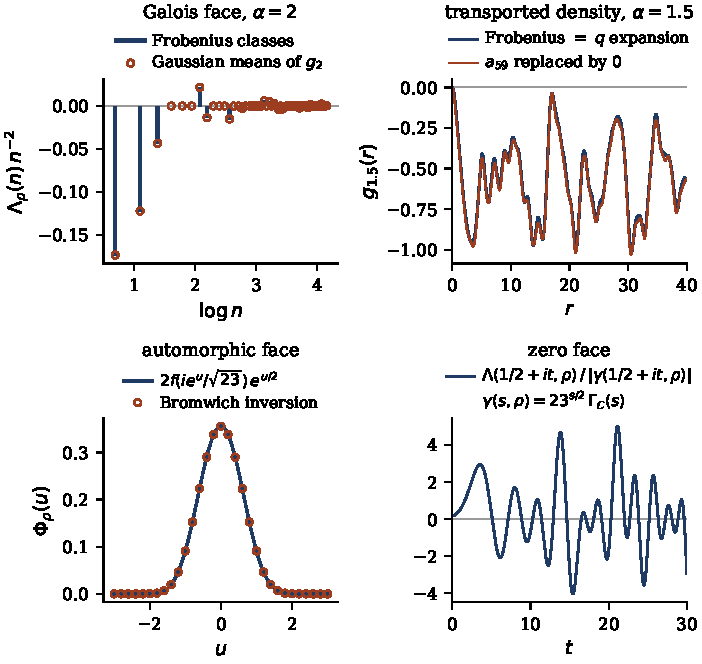
\includegraphics[width=\textwidth]{figs/lap_faces.pdf}
\caption{Four faces of $L(s,\rho)=L(s,\eta(z)\eta(23z))$, $\rho$ the two dimensional representation of the Galois group of the splitting field of $x^3-x-1$. Top left: the Galois face at $\alpha=2$, the atoms $\Lambda_\rho(n)n^{-2}$, $n\le64$, from Frobenius classes (bars) and as Gaussian means of the transported density $g_2$ computed from the modular form (circles), Corollary~\ref{cor:lapfrob}. Top right: the transport face, the transported density $g_{1.5}$ from Frobenius and from the $q$ expansion (one curve, the two being identical), and with $a_{59}$ replaced by $0$. Bottom left: the automorphic face, the kernel $\Phi_\rho$ computed by Bromwich inversion of $\Lambda(\frac12+it,\rho)$ (circles) against $2f(ie^u/\sqrt{23})e^{u/2}$ for $f=\eta(z)\eta(23z)$ (line), Proposition~\ref{prop:lappolya}. Bottom right: for the zero face, the zeros themselves, as the sign changes of the real function $\Lambda(\frac12+it,\rho)/|\gamma(\frac12+it,\rho)|$, with $\gamma(s,\rho)=23^{s/2}\Gamma_\C(s)$ the gamma factor of Section~\ref{sec:10bcompletion}, of absolute value $|L(\frac12+it,\rho)|$.}\label{fig:lapfaces}
\end{figure}

\section{Bromwich inversion: from the Artin \texorpdfstring{$L$}{L} function to the modular form}\label{sec:lappolya}

The automorphic face of a degree two $L$ function is a function on the imaginary axis, and the Mellin transform makes it a two sided Laplace transform, as in Section~\ref{sec:02mellin} and \eqref{eq:recipmellin}. Write $\Gamma_\C(s)=2(2\pi)^{-s}\Gamma(s)=\Gamma_\R(s)\Gamma_\R(s+1)$.

\begin{proposition}[Mellin inversion of an Artin $L$ function; after Hecke \cite{hecke1936}]\label{prop:lappolya}
Let $\rho$ be an odd two dimensional Artin representation of conductor $N$, and assume that its completed $L$ function $\Lambda(s,\rho)=N^{s/2}\Gamma_\C(s)L(s,\rho)$ is entire and bounded in vertical strips (Artin's conjecture for $\rho$). Put
\[
\Phi_\rho(u)=\frac1{2\pi}\int_{\R}\Lambda(\tfrac12+it,\rho)e^{-itu}\,dt .
\]
Then $\Lambda(\frac12+t,\rho)=\int_{\R}\Phi_\rho(u)e^{tu}\,du$ for real $t$. If $\rho$ is attached to a weight one newform $f$, then $\Phi_\rho(u)=2f(ie^u/\sqrt N)e^{u/2}$. If moreover $\Lambda(s,\rho)=\Lambda(1-s,\rho)$, then $\Phi_\rho$ is even, and if $f$ is positive on the imaginary axis then $\Phi_\rho/\Lambda(\frac12,\rho)$ is the density of a symmetric random variable.
\end{proposition}

\begin{proof}
By the functional equation $\Lambda(s,\rho)=W(\rho)\Lambda(1-s,\bar\rho)$ and the Phragm\'en Lindel\"of principle, boundedness in vertical strips gives polynomial growth of $L(\sigma+it,\rho)$ in $|t|$, uniformly for $\sigma$ in compact sets, and Stirling's formula then gives exponential decay of $\Lambda(\sigma+it,\rho)$ in $|t|$. As in the proof of Lemma~\ref{lem:10bkernel}, $\frac1{2\pi}\int_{\R}\Lambda(\frac12+x+it,\rho)e^{-(x+it)u}\,dt$ does not depend on $x$, so it equals $\Phi_\rho(u)$, it decays faster than any exponential as $u\to\pm\infty$, and $\int_{\R}\Phi_\rho(u)e^{zu}\,du=\Lambda(\frac12+z,\rho)$ for every complex $z$, which at real $z=t$ is the first statement. If $\rho$ corresponds to $f$, then $\Lambda(s,\rho)$ is twice the function $\Lambda(s)$ of Section~\ref{sec:recipfaces} with $k=1$, because $\Gamma_\C(s)=2(2\pi)^{-s}\Gamma(s)$. Both sides of the second identity in \eqref{eq:recipmellin} are entire in $t$, because $f(iy)$ decays exponentially as $y\to\infty$ and, by the Fricke involution, as $y\to0$, so that identity and the uniqueness of the Fourier transform give $\Phi_\rho=2\Phi_f$, with $\Phi_f(u)=f(ie^u/\sqrt N)e^{u/2}$ the P\'olya kernel of Chapter~\ref{ch:recip}. The last statements are Hecke's criterion (Proposition~\ref{prop:recipsym}) and positivity.
\end{proof}

The input to the integral is Galois data together with analytic continuation. An Artin $L$ function is determined by the Frobenius classes, and its meromorphic continuation and functional equation follow from Brauer's induction theorem \cite{brauer1947}; that $\Lambda(s,\rho_{23})$ is entire and bounded in strips is Hecke's theorem, since $L(s,\rho_{23})=\zeta_K(s)/\zeta(s)$, $K=\Q[x]/(x^3-x-1)$, is the $L$ function of the weight one form $\eta(z)\eta(23z)$ (Example~\ref{ex:ch3cubic}). PARI computes $\Lambda(s,\rho_{23})$ as this quotient, using the functional equations of $\zeta_K$ and $\zeta$. The output is a function on the imaginary axis, and reciprocity says that it is a modular form. We evaluated $\Lambda(\frac12+it,\rho)$ for $0\le t\le60$ in steps of $0.005$ (it is real there, and below $10^{-26}$ in absolute value beyond $t=40$), integrated, and compared $\Phi_\rho$ with $2f(ie^u/\sqrt{23})e^{u/2}$ for $f=\eta(z)\eta(23z)$, summed from $4000$ terms of its $q$ expansion. On $|u|\le3$ the two agree to $2.7\cdot10^{-16}$ in absolute value, the level of rounding (Figure~\ref{fig:lapfaces}, bottom left). The kernel is positive, with $\int\Phi_\rho=\Lambda(\frac12,\rho)=0.5390$, so $\Phi_\rho/\Lambda(\frac12,\rho)$, the P\'olya kernel\index{P\'olya kernel} $\Phi^{\mathrm{sd}}$ of Lemma~\ref{lem:10bkernel} for the weight one form, is the density of a symmetric random variable, its P\'olya variable (Chapter~\ref{ch:recip} uses $\Phi_f=\frac12\Phi_\rho$).

The proposition also says where the deep content of reciprocity sits. The inverse transform exists once $\Lambda(s,\rho)$ is entire and bounded in strips. That the result is modular, transforming correctly under all of $\Gamma_0(N)$ with its character and not merely under the Fricke involution, follows from Weil's converse theorem\index{converse theorem} (\cite{weil1967}, Satz~2) once the twists $\Lambda(s,\rho\otimes\chi)$ are also entire, bounded in strips and satisfy their functional equations; for two dimensional Artin representations this is Th\'eor\`eme~4.10 of Deligne and Serre \cite{deligneserre1974}. For odd irreducible $\rho$ these hypotheses are now known, by Hecke, Langlands and Tunnell \cite{langlands1980,tunnell1981} when the projective image is solvable and in general through Serre's conjecture, proved by Khare and Wintenberger \cite{kharewintenberger2009,kharewintenberger2009b} with work of Kisin \cite{kisin2009} (Chapter~\ref{ch:flt}).

\section{Moving the basepoint: the Cauchy semigroup}\label{sec:lapcauchy}

The Galois face lives at basepoints $\alpha>1$, the zeros at the centre. Theorem~\ref{thm:10dshift} gives a Thorin representation at every basepoint to the right of all zeros, and its proof writes the Thorin density as a sum of Poisson kernels over the zeros (see also Proposition~\ref{prop:10dsmooth} and Section~\ref{sec:sf:strip}); we now read that sum as a law. Let $\pi$ be self dual and let $\Xi^{\mathrm{sd}}_\pi(w)$ be $\Lambda(\frac12+w,\pi)$ divided by the power of $w$ that removes any zero at $w=0$, as in Definition~\ref{def:10bxi}; for $\zeta$ use $\Xi_\zeta(w)=\xi(\frac12+w)$ in its place below. Since $\Xi_\pi=(\Xi^{\mathrm{sd}}_\pi)^2$, Theorem~\ref{thm:10dshift} holds for $\Xi^{\mathrm{sd}}_\pi$ with every Thorin density halved, as in the last sentence of Theorem~\ref{thm:10bmain}, and below $V_a$ and $H_a$ denote this version. The function $\Xi^{\mathrm{sd}}_\pi$ is even and entire of order at most one (Lemma~\ref{lem:10bcompletion}(iii) and (v)); its zeros $z=\beta+i\gamma$, counted with multiplicity, form a multiset $\mathcal Z$ closed under $z\mapsto-z$ and $z\mapsto\bar z$, and $|\beta|<\frac12$. Let $C$ denote a standard Cauchy variable, with density $1/(\pi(1+x^2))$.

\begin{theorem}[zeros plus Cauchy noise; after \cite{polson2017,polson2018vdp}]\label{thm:lapcauchy}
Let $a>|\beta|$ for every $z=\beta+i\gamma$ in $\mathcal Z$; this holds unconditionally for $a\ge\frac12$. In the variable $r>0$, the square root of the Thorin variable, the Thorin measure of the GGC $H_a$ of Theorem~\ref{thm:10dshift}, $\Xi^{\mathrm{sd}}_\pi(a)/\Xi^{\mathrm{sd}}_\pi(a+\sqrt s)=\E e^{-sH_a}$, is
\[
V_a(r^2)\,2r\,dr=\frac12\sum_{z\in\mathcal Z}\operatorname{Law}\bigl(|\gamma+(a-\beta)C|\bigr)(dr),\qquad r>0 .
\]
Under GRH this is $\sum_{\gamma>0}\operatorname{Law}(|\gamma+aC|)$ for every $a>0$, a superposition of folded Cauchy laws centred at the ordinates with common scale $a$. For $b>0$, $V_{a+b}$ is obtained from $V_a$ by adding independent Cauchy noise of scale $b$ before folding, and on the Galois face, for $a>\frac12$, this is multiplication by $e^{-bx}$ of the whole L\'evy measure of $\log\Xi^{\mathrm{sd}}_\pi$ at basepoint $a$, archimedean and polynomial factors included.
\end{theorem}

\begin{proof}
By the definition of $V_a$ in Theorem~\ref{thm:10dshift}, $V_a(r^2)\,2r=\frac1\pi\operatorname{Re}(\log\Xi^{\mathrm{sd}}_\pi)'(a+ir)$, and by the Hadamard product $(\log\Xi^{\mathrm{sd}}_\pi)'(w)$ is the sum of $(w-z)^{-1}$ over $z\in\mathcal Z$, taken in pairs $\pm z$. For $z=\beta+i\gamma$,
\[
\frac1\pi\operatorname{Re}\frac1{a+ir-z}=\frac1\pi\frac{a-\beta}{(a-\beta)^2+(r-\gamma)^2},
\]
the density at $r$ of $\gamma+(a-\beta)C$, positive because $a>|\beta|$. The symmetries of $\mathcal Z$ make the sum even in $r$, so on $r>0$ it is half the sum of the folded densities, as stated. Under GRH, $\mathcal Z=\{\pm i\gamma\}$, $\beta=0$, and the two zeros $\pm i\gamma$ give the two halves of $\operatorname{Law}(|\gamma+aC|)$. Cauchy laws are stable, $(a-\beta)C+bC'$ having the law of $(a+b-\beta)C$ for independent $C,C'$, which is the semigroup. On the Galois face, for $a>\frac12$ the L\'evy measure of $\log\Xi^{\mathrm{sd}}_\pi$ at basepoint $a$ is $e^{-ax}\mu(dx)/x$ with $\mu$ independent of $a$, as in \eqref{eq:10dlk} with $\nu$ now signed, so moving to $a+b$ multiplies it by $e^{-bx}$; and $e^{-b|x|}$ is the Fourier transform of the Cauchy density of scale $b$.
\end{proof}

The Poisson kernel form of $V_a$ is in the proof of Theorem~\ref{thm:10dshift} and in Proposition~\ref{prop:10dsmooth}, for $\xi$ in \cite{polson2018vdp} (Theorem~18 and Remark~21), and Chapter~\ref{ch:squarefree} writes the density contributed by a pair of zeros off the line as a sum of two Poisson kernels (Section~\ref{sec:sf:strip}); the semigroup\index{Cauchy semigroup} in the basepoint is the backward Cauchy flow of \cite{polson2017} (Section~8 and Theorem~9.2). The theorem states these facts through folded Cauchy variables and for every self dual $\pi$; for $\xi$, its distribution function is the sum of arctangents of Theorem~8.2 of \cite{polson2017}. We check it below against $1000$ zeros of $\zeta$. Chapter~\ref{ch:scholze} smooths the atoms at the squared ordinates by Lorentzians of width $\varepsilon$, through Stieltjes inversion; here the smoothing is in the variable $r$, its scale is $a-\beta$, and it comes from moving the basepoint.

The theorem gives a probabilistic picture of the passage from the Galois face to the zeros. At $a\ge\frac12$, where the Thorin measure is positive unconditionally, each zero is seen through Cauchy noise of scale between $a-\frac12$ and $a+\frac12$. As $a$ decreases the noise shrinks, and GRH is the statement that it can be shrunk to zero for every zero at once; a zero with $\beta>0$ would make the scale $a-\beta$ negative for $a<\beta$, a negative Cauchy density. The proof of Theorem~\ref{thm:10dshift}(iv) and the remark after it use this sign change, and the criterion of Hinkkanen and Lagarias \cite{hinkkanen1997,lagarias1999}, that the Riemann hypothesis holds if and only if $\operatorname{Re}\xi'/\xi(s)>0$ for $\operatorname{Re}s>\frac12$, is the same statement about scales: its proof (\cite{lagarias1999}, Section~2) adds the same Poisson kernels term by term.

For $\zeta$ we compared $\frac1\pi\operatorname{Re}(\Xi_\zeta'/\Xi_\zeta)(a+ir)$ on $0<r\le50$, computed from $\zeta$, $\Gamma$ and the polynomial factor, with the Cauchy superposition over the first $1000$ zeros plus a smooth tail beyond $\gamma_{1000}=1419.42$. The maximal differences are $9.2\cdot10^{-8}$, $3.7\cdot10^{-8}$ and $9.2\cdot10^{-9}$ at $a=0.5$, $0.2$ and $0.05$, against peak values $0.72$, $1.63$ and $6.37$ (Figure~\ref{fig:lapzeta}, left).

\section{Inverting the Thorin law: a universal tail}\label{sec:laptail}

The Thorin variable $H$ of Lemma~\ref{lem:10dsin2} is the second member of a Wald couple of Roynette and Yor \cite{roynetteyor2005}, who found the tail of its density. Inverting the Laplace transform recovers their result, and the inversion has a universal feature.

\begin{theorem}[the tail of the Thorin variable; Roynette and Yor \cite{roynetteyor2005}]\label{thm:laptail}
Let $\Lambda_f(n)\ge0$, not all zero, and let $f(s)=\exp\bigl(\sum_{n\ge2}\Lambda_f(n)n^{-s}/\log n\bigr)$ converge absolutely for $\operatorname{Re}s>\alpha_0$. For $\alpha>\alpha_0$ let $H$ be the GGC of Lemma~\ref{lem:10dsin2} for $f$ at the basepoint $\alpha$, with $\nu_\alpha=\sum_n\Lambda_f(n)n^{-\alpha}\delta_{\log n}$, so that
\[
\E e^{-sH}=e^{b\sqrt s}\,\frac{f(\alpha)}{f(\alpha+\sqrt s)},\qquad b=\frac{f'}f(\alpha)<0 .
\]
Then
\[
\E H=\tfrac12(\log f)''(\alpha),\qquad \E H^2=\infty,
\]
and the density $p$ of $H$ satisfies
\[
p(t)\sim A\,t^{-5/2},\qquad \Prob(H>t)\sim\tfrac23A\,t^{-3/2},
\]
where
\[
A=\frac{-(\log f)'''(\alpha)}{8\sqrt\pi}=\frac1{8\sqrt\pi}\sum_n\frac{\Lambda_f(n)(\log n)^2}{n^\alpha}.
\]
\end{theorem}

This is Proposition~I.3.1 and Remarque~I.3.2 of \cite{roynetteyor2005} for $c(dx)=\nu_\alpha(dx)/x$, their $H$ being $2H$ here, with the density given by part~(1) of that proposition; for $\zeta$ the variable and its mean are their Th\'eor\`eme~V.1.1. They reach the constant through a Tauberian theorem; the proof below uses Doetsch's transfer theorem, which also gives the next terms.

\begin{proof}
Write $\varphi(s)=\E e^{-sH}$ and $w=\sqrt s$. Since $\log f$ is holomorphic near $\alpha$, Taylor's formula gives $\log f(\alpha+w)=\log f(\alpha)+bw+\frac12f_2w^2+\frac16f_3w^3+O(w^4)$ with $f_k=(\log f)^{(k)}(\alpha)$, so
\[
\log\varphi(s)=-\tfrac12f_2\,s-\tfrac16f_3\,s^{3/2}+O(s^2),
\]
uniformly as $s\to0$ in the slit plane. Differentiating the series of $\log f$ term by term gives $f_2=\sum\Lambda_f(n)\log n\,n^{-\alpha}$ and $f_3=-\sum\Lambda_f(n)(\log n)^2n^{-\alpha}<0$. The mean is the coefficient of $-s$. The term $s^{3/2}$ is not twice differentiable at $0$, so $\E H^2=\infty$. The function $\varphi$ is holomorphic on $\C\setminus(-\infty,0]$, because $\operatorname{Re}\sqrt s>0$ there and $f$ has no zeros on $\operatorname{Re}s>\alpha_0$, and $\varphi(s)\to0$ as $|s|\to\infty$, uniformly in every sector $|\arg s|\le\pi-\delta$, since $f(\alpha+\sqrt s)\to1$ and $b<0$. Since $\log f(\alpha+w)$ is analytic in $w$, the expansion of $\varphi$ at $0$ is a power series in $\sqrt s$, so after $s^{3/2}$ the next nonintegral power is $s^{5/2}$. Doetsch's transfer theorem for Laplace transforms with algebraic singularities \cite{doetsch1974}, whose hypotheses are these two properties, turns each term $cs^\lambda$, $\lambda\notin\{0,1,2,\dots\}$, of the expansion at $0$ into a term $ct^{-\lambda-1}/\Gamma(-\lambda)$ of the density at infinity. With $c=-f_3/6$, $\lambda=\frac32$ and $\Gamma(-\frac32)=\frac43\sqrt\pi$ this is $A$. Integrating gives the tail of the distribution function.
\end{proof}

The index $\frac32$ does not depend on $f$ or on $\alpha$. By Step~3 of the proof of Lemma~\ref{lem:10dsin2}, $H$ has the L\'evy density
\[
\frac{k(y)}y=\frac1{2\sqrt\pi\,y^{3/2}}\int_0^\infty\bigl(1-e^{-x^2/(4y)}\bigr)\,\nu_\alpha(dx)\sim Ay^{-5/2},\qquad y\to\infty,
\]
since $1-e^{-x^2/(4y)}\sim x^2/(4y)$: the L\'evy measure already has the tail of the theorem, the power coming from the stable law of index $\frac12$ in Step~1, and the theorem says that the law inherits it. What depends on the arithmetic is the constant, $(8\sqrt\pi)^{-1}$ times the second moment $\int x^2\nu_\alpha(dx)$ of the Galois face. Since $8\sqrt\pi A(\alpha)=\sum_n\Lambda_f(n)(\log n)^2n^{-\alpha}$ is a Dirichlet series, the function $\alpha\mapsto A(\alpha)$ on an interval determines $\Lambda_f$, by Theorem~\ref{thm:laplerch}.

The variable $H_a$ of Theorem~\ref{thm:lapcauchy}, for $\Xi=\Xi^{\mathrm{sd}}_\pi$ or $\Xi_\zeta$, is not compensated: its transform $\Xi(a)/\Xi(a+\sqrt s)$ contains the factor $e^{-b_a\sqrt s}$ of a positive stable law of index $\frac12$, with $b_a=(\Xi'/\Xi)(a)>0$. So $\Prob(H_a>t)\sim b_a/\sqrt{\pi t}$ for every $a$ to which Theorem~\ref{thm:10dshift}(i) applies (every $a\ge\frac12$, and every $a>0$ under GRH), while under GRH the limit at $a=0$, the explosion time of Theorem~\ref{thm:hitexplosion}, has an exponential tail. With that factor removed, $e^{b_a\sqrt s}\,\Xi(a)/\Xi(a+\sqrt s)$ is a GGC transform exactly when the density $V_a-b_a/(2\pi\sqrt z)$ is nonnegative, which for $\xi$ holds under the Riemann hypothesis, is known unconditionally for $\frac12+a\ge1$, and is open below (Section~\ref{sec:10daway}, Open Problem~\ref{op:recipdescent}). Where it holds, the proof of Theorem~\ref{thm:laptail} applies with $f=\Xi$ at the basepoint $a$, the decay of the transform in sectors now coming from Stirling's formula: the compensated variable has the density tail $A_at^{-5/2}$, $A_a=-(\log\Xi)'''(a)/(8\sqrt\pi)$, which for $\xi$ is positive whenever $\frac12+a<24$.

For $\zeta$ at $\alpha=2$ we inverted $\varphi$ by Talbot's method on $0.0005\le t\le400$ (Figure~\ref{fig:lapzeta}, right). Here $b=-0.569961$, $\E H=\frac12(\log\zeta)''(2)=0.442241$ and $A=0.137531$. The computed density has mass $0.99999$ on $[0.0005,400]$, the rest being $\Prob(H>400)\approx\frac23A\cdot400^{-3/2}=1.15\cdot10^{-5}$, and mean $0.4285$ there, which with $0.0137$ from the tail $At^{-5/2}$ beyond $400$ gives $\E H=0.4422$. The ratios $p(t)t^{5/2}/A$ are $0.991$, $0.996$, $0.998$, $0.999$ at $t\approx50$, $100$, $200$, $400$, approaching $1$ like $1/t$. The Post Widder approximations of Theorem~\ref{thm:lappostwidder} at $t=0.05$ are $4.025$, $4.455$ and $4.551$ for $k=4$, $16$ and $32$, against the Talbot value $4.657$, an error decreasing roughly like $1/k$.

\begin{figure}[!htbp]
\centering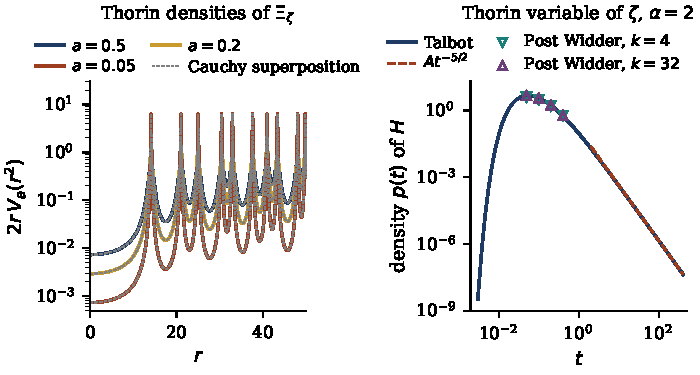
\includegraphics[width=\textwidth]{figs/lap_zeta.pdf}
\caption{Left: Theorem~\ref{thm:lapcauchy} for $\zeta$, the densities $2rV_a(r^2)$ of $\Xi_\zeta$ (Thorin densities for $a\ge\frac12$, and under the Riemann hypothesis below) at basepoints $a=0.5$, $0.2$, $0.05$ (those of $\xi$ at $\frac12+a$), with the Cauchy superpositions over the zeros drawn on top in grey dashed lines; the two agree to $10^{-7}$. Right: Theorem~\ref{thm:laptail}, the density of the Thorin variable of $\zeta$ at $\alpha=2$ by Talbot inversion, its tail $At^{-5/2}$, and the Post Widder approximations with $k=4$ and $32$, on logarithmic axes.}\label{fig:lapzeta}
\end{figure}

\section{Perron's formula as Bromwich inversion}\label{sec:lapperron}

The oldest passage between the two descriptions is classical, and we record it in the language of this chapter; Chapter~\ref{ch:squarefree} uses the same contour shift in \eqref{eq:sf:perron}, for the squarefree ideals of a number field. The undamped Galois face of $\zeta$ is the measure $\nu_0=\sum_n\Lambda(n)\delta_{\log n}$, whose distribution function is Chebyshev's $\psi(e^u)=\sum_{n\le e^u}\Lambda(n)$, and $-\zeta'/\zeta(s)=\int e^{-su}\,d\psi(e^u)$ is its Laplace Stieltjes transform. Bromwich inversion on a line $\operatorname{Re}s=c>1$, taken as a symmetric principal value since $x^s/s$ is not integrable on the line, is Perron's formula \cite{perron1908},
\[
\psi(x)=\frac1{2\pi i}\int_{c-i\infty}^{c+i\infty}\Bigl(-\frac{\zeta'}\zeta(s)\Bigr)\frac{x^s}s\,ds,\qquad x>1\text{ not a prime power},
\]
in which only Galois data enter. Moving the contour to the left across the critical strip, the integrand meets the pole at $s=1$, the zeros $\rho$, the pole at $s=0$, which gives $-\log2\pi$, and the trivial zeros, which give $-\frac12\log(1-x^{-2})$, and the residues give the explicit formula (\cite{davenport2000}, Chapter~17), the sum over $\rho$ being the limit of the sums over $|\gamma|<T$ as $T\to\infty$:
\[
\psi(x)=x-\sum_\rho\frac{x^\rho}\rho-\log2\pi-\tfrac12\log(1-x^{-2}).
\]
The contour shift is the passage: on $\operatorname{Re}s>1$ the integrand is an Euler product, and to the left of the critical strip it is controlled by the functional equation, which for $\zeta$ is the modularity of the theta function. The Cauchy semigroup of Section~\ref{sec:lapcauchy} reaches the zeros by moving a basepoint instead of a contour, with positive measures wherever Theorem~\ref{thm:10dshift}(i) applies. The explicit formula is also used in Section~\ref{sec:05bias} and Chapter~\ref{ch:recip}.

\section{Splines, P\'olya frequency functions and roughness penalties}\label{sec:lapspline}

Two classical papers sit exactly on the arrows of this chapter. Curry and Schoenberg \cite{curryschoenberg1966}, in the full version of their 1947 announcement, developed the fundamental splines, now called B splines, proved that they are probability densities, the volumes of the sections of a simplex, and studied their limits, which are Schoenberg's P\'olya frequency functions \cite{schoenberg1951}, totally positive of every order. Good and Gaskins \cite{goodgaskins1971} estimated a probability density $f$ by maximising the log likelihood minus a roughness penalty $\mathcal R(f)=\omega_1\int(\sqrt f)'^2+\omega_2\int(\sqrt f)''^2$, whose first term is $\frac{\omega_1}4$ times the Fisher information for location, $\int f'^2/f=4\int(\sqrt f)'^2$; they read $e^{-\mathcal R}$ as a prior \cite{goodgaskins1971,goodgaskins1980}, and their second paper used the method to hunt for bumps. De Montricher, Tapia and Thompson \cite{demontrichertapiathompson1975} showed (Proposition~3.5) that with the first penalty alone the estimate is an exponential spline with knots at the observations. So the two papers meet through splines, and both meet the inverse Laplace transforms of this chapter. Inverting a GGC with finitely many Thorin atoms gives a Gamma variable times a B spline variable, Schoenberg's theorem turns GRH into a P\'olya frequency statement (Chapter~\ref{ch:10d}), and among densities vanishing on the walls the Good and Gaskins penalty singles out the Sato Tate law.

\subsection{Atomic Thorin laws invert to B splines}

For $k\ge1$ and knots $u_0\le\dots\le u_k$ with $u_0<u_k$ the Curry Schoenberg B spline is $M(x;u_0,\dots,u_k)=k\,[u_0,\dots,u_k](\cdot-x)_+^{k-1}$, the divided difference in the first variable, read as a confluent one at repeated knots. It is a probability density on $[u_0,u_k]$, and it is the density of $\sum_iu_iP_i$ with $(P_0,\dots,P_k)$ uniform on the simplex, that is Dirichlet with all parameters $1$: the spline is the shadow of a simplex \cite{curryschoenberg1966}. Both facts follow from the classical Hermite Genocchi formula $[u_0,\dots,u_k]\phi=\frac1{k!}\E\phi^{(k)}(\sum_iu_iP_i)$ \cite{deboor2005}.

\begin{theorem}[atomic Thorin laws are Gamma times B spline; after \cite{curryschoenberg1966,jamesroynetteyor2008}]\label{thm:lapspline}
Let $k\ge1$, $0<c_0\le\dots\le c_k$ with $c_0<c_k$, and $H=\sum_iE_i/c_i$ with independent standard exponentials $E_i$, the GGC with Thorin measure $\sum_i\delta_{c_i}$.
\begin{enumerate}
\item[(a)] $H$ has the law of $Y_{k+1}D$, with $Y_{k+1}$ Gamma of shape $k+1$ independent of $D$, whose density is the B spline with knots $1/c_0,\dots,1/c_k$.
\item[(b)] The inverse Laplace transform of $\prod_i(1+s/c_i)^{-1}$ is
\begin{align*}
p_H(t)&=\Bigl(\prod_ic_i\Bigr)(-1)^k[c_0,\dots,c_k]e^{-t\,\cdot}\\
&=\Bigl(\prod_ic_i\Bigr)\frac{t^k}{k!}\int_{c_0}^{c_k}e^{-tx}M(x;c_0,\dots,c_k)\,dx,
\end{align*}
that is $(\prod_ic_i)t^k/k!$ times the Laplace transform of the B spline with knots $c_0,\dots,c_k$. Repeated atoms give repeated knots, with the divided difference read as a confluent one.
\end{enumerate}
\end{theorem}

\begin{proof}
(a) With $Y_{k+1}=\sum_iE_i$ and $P_i=E_i/Y_{k+1}$, $Y_{k+1}$ is Gamma of shape $k+1$, $(P_0,\dots,P_k)$ is Dirichlet with all parameters $1$, and the two are independent by the beta gamma algebra (\cite{jamesroynetteyor2008}, Section~1.4). Then $H=Y_{k+1}D$ with $D=\sum_iP_i/c_i$, which has the B spline density with knots $1/c_i$. (b) For distinct atoms, partial fractions give $p_H(t)=(\prod_jc_j)\sum_ie^{-c_it}/\prod_{j\ne i}(c_j-c_i)$, which is the divided difference written; repeated atoms follow by continuity in the $c_i$. Hermite Genocchi with $\phi(x)=e^{-tx}$, $\phi^{(k)}=(-t)^ke^{-tx}$, gives the second form.
\end{proof}

Part~(a) is the atomic case of the factorisation of James, Roynette and Yor \cite{jamesroynetteyor2008} (Section~1.4, equation~(33)): a GGC whose Thorin measure has finite mass $m$ is a Gamma variable of shape $m$ times an independent Dirichlet mean, by the beta gamma algebra. In part~(b) the first form is the classical density of a sum of independent exponentials, written as a divided difference, and the second is its Peano kernel form \cite{deboor2005}. So inverting the Laplace transform of an atomic Thorin law is a divided difference, and a divided difference is an expectation over a simplex. When the Thorin measure is the image under $1/Q$ of a probability measure $\mu$ restricted to $\{Q>0\}$, as for the Frobenius functionals of Chapter~\ref{ch:recip}, the factorisation can also be written with a standard exponential variable and the Dirichlet mean $\int Q\,dP$ of a Dirichlet process $P$ with base measure $\mu$, and Chapter~\ref{ch:pd} identifies $P$ with the limit of the normalised labelled factorisation of a random integer (Theorem~\ref{thm:pddirichlet}).

For the Hecke GGC $H_N(\ell)$ of Definition~\ref{def:flthecke}, whose $g$ atoms $\ell+1-a_\ell(f)$ have product $|J_0(N)(\mathbb F_\ell)|$ (Chapter~\ref{ch:flt}), part~(b) gives
\[
p_{H_N(\ell)}(t)=|J_0(N)(\mathbb F_\ell)|\,\frac{t^{g-1}}{(g-1)!}\int e^{-tx}M\bigl(x;\{\ell+1-a_\ell(f)\}_f\bigr)\,dx :
\]
the density of the Hecke variable is $t^{g-1}$ times the Laplace transform of a B spline whose knots are the atoms. The atom of a rational $f$, attached to an elliptic curve $E_f$, is the point count $|E_f(\mathbb F_\ell)|$, but only the product of all the atoms is always a point count. Hecke atoms can repeat, for example at $(N,\ell)=(37,7)$ and $(113,2)$, and then the knots repeat; at $(37,7)$ both atoms are $9$, the B spline degenerates to the point mass at $9$, and $H_{37}(7)$ is a Gamma variable of shape $2$ and rate $9$. For $N=67$, $\ell=2$, the five atoms are $1$, $2.382$, $3.382$, $4.618$, $5.618$ with product $209=|J_0(67)(\mathbb F_2)|$. Computed exactly, the B spline formula agrees with the partial fraction density to within $6\cdot10^{-15}$ on $[0,4]$, and a histogram of $400000$ samples of $Y_5D$ agrees with both within sampling error (Figure~\ref{fig:lapspline}, right).

\subsection{P\'olya frequency functions and GRH}

Schoenberg's theorem (Theorem~\ref{thm:ch10schoenberg}) characterises the P\'olya frequency functions, totally positive of every order, by their bilateral Laplace transforms, the reciprocals of functions of the Laguerre P\'olya class, and Curry and Schoenberg showed that these functions arise as limits of their B splines \cite{curryschoenberg1966}. Through Schoenberg's theorem, Theorem~\ref{thm:10dvdp} and the remark after its proof show that GRH for $\pi$ holds if and only if $t\mapsto\Xi_\pi(0)/\Xi_\pi(t)$ is the characteristic function of a symmetric P\'olya frequency density, that of $V_\pi=\sum_kL_k/\gamma_k$, with independent standard Laplace variables $L_k$, which has the law of $\sqrt{2Z_\pi}\,N$, where $Z_\pi$ is the explosion time of Theorem~\ref{thm:hitexplosion} and $N$ is standard normal and independent of $Z_\pi$ (for $\xi$, \cite{roynetteyor2005,polson2018vdp,konstantopoulospatiesarkar2024}). Under GRH the density of $V_\pi$ is therefore a limit of B spline densities, and its truncation to the first $K$ zeros is a difference $\sum_{k\le K}E_k/\gamma_k-\sum_{k\le K}E'_k/\gamma_k$ of two independent hypoexponential variables, each a Gamma variable times a B spline variable by Theorem~\ref{thm:lapspline}. The bilateral Laplace transform of $V_\pi$ is $\E e^{sV_\pi}=\E e^{s^2Z_\pi}$, the transform of the explosion time continued to negative argument.

\subsection{The Sato Tate law minimises the Good and Gaskins penalty}

Let $G$ be a compact connected simply connected Lie group, such as $\SU(2)$ or $\USp(2n)$, with alcove $\mathcal A$, positive roots $\alpha$ and half sum $\rho_G$, and give the Lie algebra of a maximal torus the invariant inner product in which, for $\SU(2)$ and $\USp(2n)$, the eigenvalue angles are orthonormal coordinates. By Weyl's integration formula (Theorem~\ref{thm:ch6weyl}) the image of Haar measure on conjugacy classes, the Sato Tate law of Chapter~\ref{ch:04} for $\SU(2)$ and of Chapter~\ref{ch:12} for $\USp(4)$, has density $f_G=c|\Delta_G|^2$ on $\mathcal A$, with $\Delta_G=\prod_{\alpha>0}(e^{i\alpha/2}-e^{-i\alpha/2})$. By the Weyl character formula $\Delta_G\chi_\lambda=\sum_w\operatorname{sgn}(w)e^{iw(\lambda+\rho_G)}$, an eigenfunction of the Laplacian with eigenvalue $|\lambda+\rho_G|^2$ that vanishes on the walls of $\mathcal A$; for $\lambda=0$ it has constant sign inside $\mathcal A$.

\begin{theorem}[Sato Tate is the Good and Gaskins ground state; this book, after \cite{huber1974,berard1980}]\label{thm:lapgg}
Among densities $f$ on $\mathcal A$ such that $\sqrt f$ vanishes on the boundary $\partial\mathcal A$ and $\int_{\mathcal A}|\nabla\sqrt f|^2<\infty$, the Good and Gaskins roughness $\int_{\mathcal A}|\nabla\sqrt f|^2$, one quarter of the trace of the Fisher information for location, is at least $|\rho_G|^2$, with equality exactly for the Sato Tate law $f_G$. For $G=\SU(2)$, with $\theta\in[0,\pi]$ and $\sqrt f=\sqrt{2/\pi}\sum_jb_j\sin j\theta$, $\sum_jb_j^2=1$,
\[
\int_0^\pi\bigl((\sqrt f)'\bigr)^2d\theta=\sum_jj^2b_j^2,\qquad \frac{\sin j\theta}{\sin\theta}=\tr\Sym^{j-1}\begin{pmatrix}e^{i\theta}&0\\0&e^{-i\theta}\end{pmatrix},
\]
so the roughness is the Laplace eigenvalue energy $\sum_\lambda|\lambda+\rho_G|^2b_\lambda^2$, which is $|\rho_G|^2$ plus the Casimir energy, in the basis of symmetric power characters, and the Sato Tate law is $b=e_1$. Given angles $\theta_1,\dots,\theta_n$, put $\hat m_j=\frac1n\sum_{i=1}^n\tr\Sym^{j-1}(\theta_i)$, the trace being that of the matrix above. Near the Sato Tate law, the maximiser of $\frac1n\sum_i\log f(\theta_i)-\omega\int_0^\pi(\sqrt f)'^2$ over $\sqrt f=\sqrt{2/\pi}\sum_{j\le J}b_j\sin j\theta$ satisfies
\[
b_j=\frac{\hat m_j}{2+\omega(j^2-1)}+O\Bigl(\max_{2\le l\le2J-1}\hat m_l^2\Bigr),\qquad 2\le j\le J .
\]
\end{theorem}

\begin{proof}
The functions $\Delta_G\chi_\lambda$ restricted to $\mathcal A$, with $\lambda$ dominant, are a complete orthogonal system of Dirichlet eigenfunctions of the Laplacian on $\mathcal A$, by the Weyl character formula and the Peter Weyl theorem (Theorem~\ref{thm:A:pw}), with eigenvalues $|\lambda+\rho_G|^2$; the smallest is $|\rho_G|^2$, at $\lambda=0$, and it is simple. The Rayleigh quotient of $\sqrt f$, with $\int f=1$, is $\int|\nabla\sqrt f|^2\ge|\rho_G|^2$, with equality only for $\sqrt f=c|\Delta_G|$, which is $f=f_G$. For $\SU(2)$, $\mathcal A=[0,\pi]$, $\rho_G=1$, $\Delta_G\chi_{j-1}=2i\sin j\theta$, and $\int(\sum_jb_j\sqrt{2/\pi}\sin j\theta)'^2=\sum_jj^2b_j^2$. For the maximiser write $b=(\sqrt{1-|\epsilon|^2},\epsilon_2,\dots,\epsilon_J)$ and $\sin j\theta/\sin\theta=U_{j-1}(\cos\theta)$. Then $\frac1n\sum_i\log f(\theta_i)$ is a constant plus $2\sum_j\epsilon_j\hat m_j-|\epsilon|^2-\sum_{j,k}Q_{jk}\epsilon_j\epsilon_k+O(|\epsilon|^3)$, where $Q_{jk}=\frac1n\sum_iU_{j-1}(\cos\theta_i)U_{k-1}(\cos\theta_i)$ is the sum of the $\hat m_l$ over $l=|j-k|+1,|j-k|+3,\dots,j+k-1$ by the Clebsch Gordan rule, with $\hat m_1=1$, so that $Q_{jk}=\delta_{jk}+O(\max_l|\hat m_l|)$. The penalty is $\omega(1+\sum_j(j^2-1)\epsilon_j^2)$. At the stationary point $(2+\omega(j^2-1))\epsilon_j=\hat m_j+O(|\epsilon|\max_l|\hat m_l|+|\epsilon|^2)$, and $\epsilon=O(\max_l|\hat m_l|)$ gives the formula: the cross terms $\epsilon_j\epsilon_k$ have coefficients $O(\max_l|\hat m_l|)$, so they change $b$ only at second order.
\end{proof}

For $\SU(2)$ the inequality is Huber's theorem that among laws on an interval the sine squared arch has least Fisher information \cite{huber1974}; in general it is the Rayleigh principle for the Dirichlet Laplacian of the alcove, whose spectrum B\'erard computed \cite{berard1980} (Proposition~9).

For $\USp(4)$, with $\sqrt f\propto(\cos\theta_1-\cos\theta_2)\sin\theta_1\sin\theta_2=\frac12(\sin2\theta_1\sin\theta_2-\sin\theta_1\sin2\theta_2)$ on $0<\theta_2<\theta_1<\pi$, the eigenvalue is $5=|\rho_G|^2$, $\rho_G=(2,1)$, and the normalising constant is $16/\pi^2$, twice the constant of Proposition~\ref{thm:12usp4}, which integrates over the square $[0,\pi]^2$. In the Bayesian reading of Good and Gaskins, with the prior $e^{-n\omega\int(\sqrt f)'^2}$ for $n$ angles, the Sato Tate law is, formally, the mode of the prior among densities whose square root vanishes on the walls, and the posterior mode is the maximiser of the theorem. Since the fitted value of $\hat m_j$, the mean of $\tr\Sym^{j-1}$, is about $2b_j$, the posterior mode shrinks the empirical moment $\hat m_j$ by the factor $(1+\omega(j^2-1)/2)^{-1}$: the larger the representation, the stronger the shrinkage. The $\hat m_j$ are the Weyl averages $W_\rho(n)$, $\rho=\Sym^{j-1}$, of Chapter~\ref{ch:12}, and the roughness prior is a nonparametric alternative of the kind discussed there, where the Bayesian identification compares finitely many candidate groups.

Figure~\ref{fig:lapspline} fits the Good and Gaskins estimate with twelve sine terms to the Frobenius angles of two curves. For $11a1$, with the $664578$ primes below $10^7$ other than $11$, the moments $\hat m_2,\dots,\hat m_7$ are of size $4\cdot10^{-4}$, the estimate is indistinguishable from the Sato Tate law (roughness $1.0001$ at $\omega=0.01$), and the exact maximiser agrees with the first order formula to within $0.7$ percent for $j\le6$ and $\omega=0.01,0.1,1$. For the curve $E_2\colon y^2=x^3-x$ of Chapter~\ref{ch:01} (conductor $32$, complex multiplication by $\Z[i]$), with the $78497$ odd primes below $10^6$, the angle law is $\mu_{\mathrm{CM}}$, $\frac12\delta_{\pi/2}$ plus half the uniform law, so $\E\tr\Sym^{2m}=\frac12((-1)^m+1)$ (Proposition~\ref{prop:04cm}). The data give $\hat m_3=-0.0033$ and $\hat m_5=0.998$, against $0$ and $1$, and the estimate at $\omega=0.01$ has $b_5=0.334$ and a spike at $\pi/2$; at $\omega=1$ the prior pulls it back to $b_5=0.035$, close to the Sato Tate shape. Here the first order formula is only qualitative, because this curve is far from Sato Tate.

\begin{figure}[!htbp]
\centering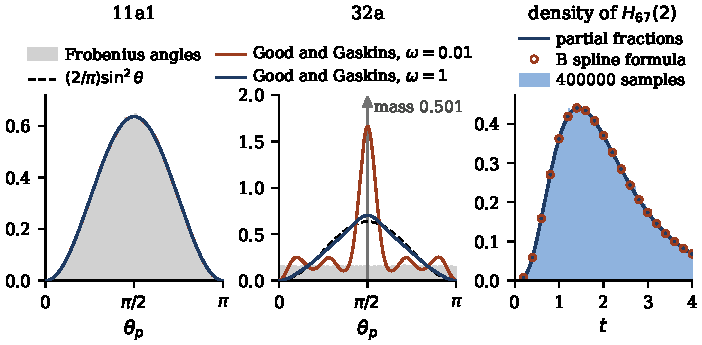
\includegraphics[width=\textwidth]{figs/lap_spline.pdf}
\caption{Left and centre: Theorem~\ref{thm:lapgg}. Good and Gaskins estimates of the Frobenius angle density with $\omega=0.01$ and $\omega=1$, against the Sato Tate law $\frac2\pi\sin^2\theta$ and over histograms of the angles, for $11a1$ (primes below $10^7$ other than $11$) and for $E_2$, of class $32a$ (odd primes below $10^6$). The atom of $E_2$ at $\pi/2$, from the primes with $a_p=0$, is drawn as an arrow labelled with its mass, and the bars show the other angles; the estimate with $\omega=0.01$ has a spike there. Right: Theorem~\ref{thm:lapspline}. The density of the Hecke GGC $H_{67}(2)$ by partial fractions and by the B spline formula computed exactly, over a histogram of $400000$ samples of a Gamma variable times a B spline variable.}\label{fig:lapspline}
\end{figure}

\subsection{Open problems}

\begin{problem}[Stable recovery of Frobenius from a window]\label{op:lapwindow}
By Theorem~\ref{thm:lapfaces}(iii) the transported density $g_\alpha$ on any interval $[0,r_0)$ determines every $\Lambda_L(n)$, but only through analytic continuation, which is unstable. Suppose $g_\alpha$ is known on $[0,r_1]$ to within $\eta$. Corollary~\ref{cor:lapfrob}, with the Gaussian mean truncated at $r_1$, recovers $\Lambda_L(n)$ to within $\varepsilon$ once $\eta$ is of order $\varepsilon n^{-\alpha}$ and $r_1$ of order $n\log(n^\alpha/\varepsilon)$. Is an interval of length of order $n$, the reciprocal of the gap $\log(1+1/n)$ between the frequencies $\log n$ and $\log(n+1)$, necessary for every stable method, as Ingham's inequality for nonharmonic Fourier series \cite{ingham1936} suggests? A positive answer would be an uncertainty principle for the Galois face, comparable with the bounds in effective Chebotarev theorems \cite{lagariasodlyzko1977}.
\end{problem}

\begin{problem}[Good and Gaskins for Thorin densities]\label{op:lapgg}
The inversions of this chapter are exact but need exact input. Treat the ordinates $0<\gamma_1\le\dots\le\gamma_K$ as a sample from the normalised counting measure of the zeros, or the transported density on a grid as noisy data; define the penalised likelihood of Good and Gaskins for the square root of the Thorin density $U_{\mathrm{ar}}$ of Section~\ref{sec:10daway}, or for the density of $H$; identify its maximiser as de Montricher, Tapia and Thompson did; and compare its error with that of the Gaussian means of Theorem~\ref{thm:lapbohr} on the same input.
\end{problem}

\section{Notes}

Lerch's theorem (Chapter~II, Theorems~6.2 and 6.3), the complex inversion formula (Chapter~II, Theorem~7.3, and Chapter~VI, Theorem~5a) and the real inversion formula, found by Post and extended by Widder (Chapter~VII), are in Widder's book \cite{widder1941}; Feller \cite{feller1971} reads the last as a law of large numbers. Talbot's contour \cite{talbot1979} and the framework of Abate and Whitt \cite{abatewhitt2006} are the standard numerical inversions, and Stieltjes inversion is classical \cite{stieltjes1894,akhiezer1965}. Theorem~\ref{thm:lapbohr} and Corollary~\ref{cor:lapfrob} are Bohr's formula for the Fourier coefficients of an almost periodic function and its uniqueness theorem, for Dirichlet series in Besicovitch \cite{besicovitch1932} (Chapter~I, Sections~3 and 4; Chapter~III, Section~3), and Theorem~\ref{thm:lapfaces} combines them with the uniqueness of Dirichlet series. Proposition~\ref{prop:lappolya} is Hecke's Mellin integral (\cite{hecke1936}, Section~2), which goes from the $L$ function to the form, the reverse of Section~\ref{sec:02mellin} and \eqref{eq:recipmellin}; that the inverse transform is modular for all of $\Gamma_0(N)$ is Weil's converse theorem \cite{weil1967} (Satz~2), and for two dimensional Artin representations it is Th\'eor\`eme~4.10 of Deligne and Serre \cite{deligneserre1974}. Perron's formula is \cite{perron1908}, and the explicit formula for $\psi$ is in \cite{davenport2000}.

The $2\sin^2$ lemma is Lemma~14 of \cite{polson2018vdp} (see also \cite{polson2017}, Section~5), with its first step from Roynette and Yor \cite{roynetteyor2005}, Th\'eor\`eme~I.1.1, as recorded in Chapter~\ref{ch:10d}, where its Thorin consequences are developed. The Poisson kernel form of Theorem~\ref{thm:lapcauchy} is in the proof of Theorem~\ref{thm:10dshift}, in Proposition~\ref{prop:10dsmooth} and in \cite{polson2018vdp} (Theorem~18 and Remark~21), and the backward Cauchy flow is in \cite{polson2017} (Section~8 and Theorem~9.2), whose Theorem~8.2 writes, for $\xi$, the distribution function of the measure of Theorem~\ref{thm:lapcauchy} as a sum of arctangents; Theorem~\ref{thm:lapcauchy} restates it through folded Cauchy variables and for every self dual $\pi$. The criterion of Hinkkanen and Lagarias \cite{hinkkanen1997,lagarias1999} adds the same Poisson kernels. The P\'olya frequency form of GRH is Theorem~\ref{thm:10dvdp}, for $\xi$ in \cite{roynetteyor2005} (Th\'eor\`eme~V.3.2), \cite{polson2018vdp} and \cite{konstantopoulospatiesarkar2024}. Theorem~\ref{thm:laptail} is due to Roynette and Yor \cite{roynetteyor2005}, whose proof is Tauberian; ours uses Doetsch's transfer theorem for Laplace transforms with algebraic singularities \cite{doetsch1974}.

The B splines and their limits are from Curry and Schoenberg \cite{curryschoenberg1966}, the Peano kernel and Hermite Genocchi forms of a divided difference are in de Boor's survey \cite{deboor2005}, P\'olya frequency functions are from Schoenberg \cite{schoenberg1951} and Karlin \cite{karlin1968}, and the Gamma times Dirichlet mean structure of GGCs, whose atomic case is Theorem~\ref{thm:lapspline}(a), is from James, Roynette and Yor \cite{jamesroynetteyor2008} (Section~1.4). The roughness penalty and its Bayesian reading are from Good and Gaskins \cite{goodgaskins1971,goodgaskins1980}, its exponential spline solutions from de Montricher, Tapia and Thompson \cite{demontrichertapiathompson1975}; Good's earlier work on Poisson summation \cite{good1962} appears in Chapter~\ref{ch:recip}. The inequality of Theorem~\ref{thm:lapgg} is Huber's for $\SU(2)$ \cite{huber1974} and the Rayleigh principle for the alcove in general \cite{berard1980}, the ground state being the Weyl denominator. New here as formulated, as far as we know, are the Gaussian error bounds of Theorem~\ref{thm:lapbohr} and Corollary~\ref{cor:lapfrob}, the Hecke reading of Theorem~\ref{thm:lapspline}, the Good and Gaskins reading of the Sato Tate law in Theorem~\ref{thm:lapgg}, with its expansion in symmetric power characters and its shrinkage formula, and the computations.

\section{Exercises}

\begin{enumerate}
\item Apply Theorem~\ref{thm:lappostwidder} to $g(x)=e^{-x}$ and show that the $k$th Post Widder approximation is $(1+t/k)^{-k-1}$.
\item Use the weak form of Theorem~\ref{thm:lapstieltjes}, integrating $\frac1\pi\operatorname{Im}(\varphi'/\varphi)(-z+i\epsilon)$ against test functions, to show that the Gamma law with shape $m$, $\varphi(s)=(1+s)^{-m}$, has Thorin measure $m\delta_1$.
\item Derive the identity of Theorem~\ref{thm:lapbohr} for a single atom $\nu=c\delta_x$, and, for $\nu=\delta_1+\delta_{1.01}$, find the smallest window $R$ for which the Gaussian mean $\mathcal G_R$ recovers the weight at $x=1$ to $10^{-6}$.
\item Show that the quadruple $z,-z,\bar z,-\bar z$ of zeros of $\Xi^{\mathrm{sd}}_\pi$, $z=\beta+i\gamma$, $0<\beta<a$, contributes $\operatorname{Law}(|\gamma+(a-\beta)C|)+\operatorname{Law}(|\gamma+(a+\beta)C|)$ to the Thorin measure of Theorem~\ref{thm:lapcauchy}, of total mass $2$, the same as two zeros of $L(s,\pi)$ on the critical line in the upper half plane.
\item For the Dedekind zeta function of $\Q(i)$, compute numerically $A$ of Theorem~\ref{thm:laptail} at $\alpha=2$ and compare it with the constant for $\zeta$.
\item Show that the B spline with two knots $u_0<u_1$ is the uniform density on $[u_0,u_1]$, and deduce from Theorem~\ref{thm:lapspline} the density of $E_0/c_0+E_1/c_1$.
\item Show that the Fisher information for location of the Sato Tate angle law $\frac2\pi\sin^2\theta$ on $[0,\pi]$ is $4$, and that no density on $[0,\pi]$ vanishing at the ends has smaller Fisher information.
\item Check Perron's formula numerically for $x=100.5$ by integrating along $\operatorname{Re}s=2$, $|\operatorname{Im}s|\le T$, and observe the convergence in $T$.
\end{enumerate}

\section{Open computational problems}

The scripts named below are in \texttt{laplace/code/} (Section~\ref{sec:B:scripts}).

\begin{compproblem}[Four faces of elliptic curves]\label{cp:lapfaces}
Objective: carry out the inversions of this chapter for elliptic curves of both root numbers. Recover $\Lambda_E(n)$ for $n\le100$ from the transported density $g_\alpha$ by the Gaussian means of Corollary~\ref{cor:lapfrob}, with the smallest window that gives each value to $10^{-6}$; rebuild the P\'olya kernel $\Phi_E$ of Proposition~\ref{prop:fltsymmetric} from $\Lambda(1+it,E)$ by Bromwich inversion and compare it with the kernel summed from the $q$ expansion; and compare the densities $V_a$ of $\Xi^{\mathrm{sd}}_E$ at $a=0.5$, $0.2$ and $0.05$ with the Cauchy superpositions of Theorem~\ref{thm:lapcauchy} over the zeros. Objects and scale: $11a1$ and $37a1$, as Figure~\ref{fig:lapfaces} does for the weight one form, then one curve from each isogeny class of conductor below $100$; Dirichlet coefficients to $10^5$; basepoints $\alpha\in\{1.5,2\}$ for $L(s+\frac12,E)$, whose coefficients are $\Lambda_E(n)n^{-1/2}$; windows up to $10^3$; zeros to height $100$. Route: \texttt{switch23.py} and \texttt{switch23b.py}, with the eta quotient replaced by the $L$ function of the curve (PARI/GP \texttt{lfuncreate}, \texttt{lfunlambda} on the critical line, \texttt{lfunzeros}); Gaussian means by quadrature truncated at six windows, as in Section~\ref{sec:lapbohr}, with the bound of Corollary~\ref{cor:lapfrob} for a finite window and a separate bound for the truncation. Deliverable: tables of the recovered $\Lambda_E(n)$, their errors and the minimal windows against $n$, with a fitted law for the window, the numerical side of Open Problem~\ref{op:lapwindow}; the maximal difference of the two kernels on $|u|\le3$, the kernel of $37a1$ being odd; and the residuals of the Cauchy superpositions. Why it matters: the Frobenius traces of the weight one form take three values at the unramified primes, while for an elliptic curve they follow the Sato Tate law and the kernels have both parities, so the problem tests the inverse arrows on the forms that carry the modularity of Chapter~\ref{ch:flt}, and it measures how pessimistic the bound of Corollary~\ref{cor:lapfrob} is.
\end{compproblem}

\begin{compproblem}[Zeros from the heat trace by Post Widder]\label{cp:lappw}
Objective: invert the heat trace by the Post Widder formula. With $N(t)$ the number of ordinates $\gamma>0$ with $\gamma^2\le t$, $\mathcal W(x)/x=\int_0^\infty e^{-xt}N(t)\,dt$, and the identity of Theorem~\ref{thm:lappostwidder}, which holds for $g$ of polynomial growth such as $N$, writes the $k$th approximation as a Gamma smoothing of $N$ of relative width about $k^{-1/2}$; find the order $k$ and the working precision at which the step of $N$ at the $j$th zero is resolved. Objects and scale: $L(s,\Delta)$, $\zeta$ and $L(s,\rho)$ for the $S_3$ representation of $x^3-x-1$; the first $50$ ordinates; orders $k\le10^3$. Route: $\mathcal W$ and its derivatives from the primes through the explicit formula \eqref{eq:10dweil}, or from Frobenius traces through Definition~\ref{def:recipheat}, in ball arithmetic, the pipeline of the derivative tests of Problem~\ref{cp:recipicosa}; the sums over the zeros as a check. Deliverable: for each function and each $j\le50$ the smallest $k$ and the precision that resolve the $j$th step, compared, at equal cost, with the Gaussian bump of Figure~\ref{fig:10dprimes} and the Cauchy smoothing of Theorem~\ref{thm:lapcauchy}. Why it matters: the derivatives $(-1)^k\mathcal W^{(k)}$ are the quantities whose signs the complete monotonicity criteria of Theorems~\ref{thm:10bmain} and \ref{thm:recipcm} concern; the problem measures how much of the zero set a given number of them determines, and whether the slow convergence of Post Widder, an error of order $1/k$, can be paid for by the accuracy of the explicit formula at small $x$.
\end{compproblem}

\begin{compproblem}[Thorin laws in the strip by Talbot inversion]\label{cp:laptalbot}
Objective: for a completed $L$ function $f$ and basepoints $\alpha$ inside and to the right of the critical strip, invert by Talbot's contour the transform $\varphi_\alpha(s)=e^{b\sqrt s}f(\alpha)/f(\alpha+\sqrt s)$, $b=(f'/f)(\alpha)$, whose Thorin density is the density $U$ of \eqref{eq:10dU}; record where the inverted density is negative, and compare its mean and its tail with $\frac12(\log f)''(\alpha)$ and with the constant $-(\log f)'''(\alpha)/(8\sqrt\pi)$ of the proof of Theorem~\ref{thm:laptail}. Objects and scale: $\xi$, $\Lambda(s,\Delta)$ at the same offsets $\alpha-\frac12$ from its centre, and $\Lambda(s,\chi_{-4})$; the basepoints $0.55$, $0.75$, $0.99$, $1.25$ and $2$ of Section~\ref{sec:10daway}; $5\cdot10^{-4}\le t\le10^4$. Route: \texttt{zeta\_tail.py}, which does this for $\zeta$ at $\alpha=2$, with $\zeta$ replaced by the completed function, $f$ and $f'/f$ from mpmath or PARI/GP \texttt{lfunlambda} at $30$ digits; Talbot's contour checked against the Euler algorithm of Abate and Whitt \cite{abatewhitt2006}; error bounds from the size of $\varphi_\alpha$ on the contour. Deliverable: the densities with their minima, total masses and means, fitted tail constants with standard errors against the predicted ones, and for each function the smallest basepoint at which the computed density is positive on the grid. Why it matters: Theorem~\ref{thm:laptail} needs nonnegative Dirichlet coefficients; for a completed function $\varphi_\alpha$ is a GGC transform exactly where $U\ge0$, which for $\xi$ holds under the Riemann hypothesis, is known for $\alpha\ge1$ and is open below (Section~\ref{sec:10daway}, Open Problem~\ref{op:recipdescent}); the inverted laws are the probabilistic content of that positivity, and a density positive on a grid verifies nothing about the zeros.
\end{compproblem}

\chapter[Random Integers and the Poisson Dirichlet Law]{Random Integers, the Poisson Dirichlet Law\\ and Chebotarev as a Dirichlet Process}\label{ch:pd}

Chapter~\ref{ch:recip} built a Gamma process from the prime factors of a zeta distributed random integer, and Chapter~\ref{ch:hit} computed the laws of the labels of its largest prime factors. Both are known objects under other names, some of which Chapter~\ref{ch:recip} recalled (Billingsley, Lloyd \cite{lloyd1984}), and this chapter develops them. The normalised sizes of the prime factors of a random integer converge to the Poisson Dirichlet law with parameter $1$, the limit law of the normalised cycle lengths of a uniform random permutation (Billingsley; Donnelly and Grimmett; Arratia, Barbour and Tavar\'e); the share of the largest prime factor follows Dickman's law; the number of prime factors is asymptotically normal by the theorem of Erd\H{o}s and Kac; and the Gamma process of Chapter~\ref{ch:recip}, normalised, is Ferguson's Dirichlet process. Chebotarev's theorem, in its Dirichlet density form, is then the statement that the base measure is Haar measure, and the limits of the Frobenius functionals of Chapter~\ref{ch:recip} are a standard exponential variable times a Dirichlet mean, so that the Gamma times Dirichlet mean factorisation of James, Roynette and Yor, whose atomic case is Theorem~\ref{thm:lapspline}, and Theorem~\ref{thm:recipggcfun} describe the same laws.

The results are of three kinds, and the Notes say which are known. Theorem~\ref{thm:pddirichlet} extends the Dirichlet law of the shares of Chapter~\ref{ch:recip} to the Dirichlet process limit and identifies the limit of a Frobenius functional as a standard exponential variable times a Dirichlet mean. Theorem~\ref{thm:pdtheta} shows that for the random integers weighted by the coefficients of $\zeta^\vartheta$, the ones that drive the zeta subordinator of Chapter~\ref{ch:10d}, the normalised sizes of the prime factors converge to the Poisson Dirichlet law with parameter $\vartheta$, so that powers of $\zeta$ give the whole Ewens family. Theorem~\ref{thm:pdmertens} gives the rates at which three natural colourings of the prime factors of a uniform random integer below $x$ approach Haar measure: the largest factor faster than any power of $1/\log x$ (Dawsey's theorem), the size biased factor at rate $1/\log x$, and the count of distinct factors only at rate $1/\log\log x$, the last two with explicit constants which are Mertens constants per Chebotarev class. The last rate shows in the data: among the distinct prime factors of random integers below $10^7$, the identity class of $S_3$ for $x^3-x-1$ accounts for $7.2$ percent of them against its Haar measure of $16.7$ percent, because no prime below $59$ lies in that class. Section~\ref{sec:pdprogress} then answers two questions and bounds a third from one side: the Mertens constants per class are explicit in $L(1,\chi)$ and $\frac{L'}L(1,\chi)$ (Theorem~\ref{thm:pdmertensL}); for an Euler product whose logarithm has nonnegative coefficients, given at the primes by a continuous function of equidistributed labels, the Ewens parameter is the exponent of the singularity at $s=1$ (the order of the pole when there is one), and the colouring of its random integer is the equidistribution measure weighted by that function (Theorem~\ref{thm:pdewens}); and in the Kolmogorov distance of the shares the Dirichlet process limit is approached no faster than $(\sigma-1)^{\delta_{\min}}$, because the smallest class is empty with probability of that order, which Chapter~\ref{ch:recip} found and Theorem~\ref{thm:pdrate} gives with its constant.

\section{The Poisson Dirichlet law}\label{sec:pdlaw}

Let $U_1,U_2,\dots$ be independent uniform variables on $(0,1)$ and define the stick breaking sequence $W_1=U_1$, $W_k=(1-U_1)\cdots(1-U_{k-1})U_k$. The sequence $(W_k)$ sums to $1$; its decreasing rearrangement $V_1\ge V_2\ge\dots$ has the \emph{Poisson Dirichlet law} $\mathrm{PD}(1)$, and $(W_k)$ itself is its size biased permutation, the GEM law \cite{kingman1993,pitman2006}. Two descriptions matter here. First, if $\Gamma$ is a standard Gamma subordinator on $[0,1]$, with L\'evy measure $x^{-1}e^{-x}dx$, then the ranked jumps of $\Gamma$ divided by $\Gamma(1)$ have the law $\mathrm{PD}(1)$ \cite{kingman1975}, and the quotient is independent of $\Gamma(1)$, which is standard exponential. Second, if $\pi_n$ is a uniform random permutation of $n$ letters, the ranked cycle lengths divided by $n$ converge in law to $\mathrm{PD}(1)$, a fact that goes back to Shepp and Lloyd \cite{shepplloyd1966}. Its analogue for prime factorisations is Billingsley's theorem \cite{billingsley1972}, found independently by Knuth and Trabb Pardo \cite{knuthtrabbpardo1976}; Donnelly and Grimmett \cite{donnellygrimmett1993} gave a short proof by size biased sampling, and Arratia, Barbour and Tavar\'e \cite{arratiabarbourtavare2003} treat integers and permutations together as logarithmic combinatorial structures.

\begin{theorem}[Billingsley \cite{billingsley1972}]\label{thm:pdbillingsley}
Let $n$ be uniform on $\{2,\dots,x\}$ with prime factorisation $n=\prod p_i^{e_i}$, and let $V_1(n)\ge V_2(n)\ge\dots$ be the decreasing rearrangement of the numbers $e_i\log p_i/\log n$, padded with zeros. As $x\to\infty$, $(V_1(n),V_2(n),\dots)$ converges in law to $\mathrm{PD}(1)$. In particular $\log P^+(n)/\log n$, with $P^+$ the largest prime factor, converges in law to $V_1$, whose distribution function is Dickman's function \cite{dickman1930}, $\Prob(V_1\le v)=\varrho(1/v)$, where $\varrho(u)=1$ on $[0,1]$ and $u\varrho'(u)=-\varrho(u-1)$ for $u>1$; its mean is the Golomb Dickman constant $0.62433$.
\end{theorem}

The parameter $1$ is the order of the pole of $\zeta$ at $s=1$, and the error in the convergence is at most of order $1/\log x$ (Tenenbaum \cite{tenenbaum2000}). The number of prime factors has its own limit law.

\begin{theorem}[Erd\H{o}s and Kac; Sathe and Selberg]\label{thm:pderdoskac}
Let $\omega(n)$ be the number of distinct prime factors of $n$ uniform on $\{1,\dots,x\}$. Then $(\omega(n)-\log\log x)/\sqrt{\log\log x}$ converges in law to the standard normal law \cite{erdoskac1940}. More precisely \cite{sathe1953,selberg1954}, uniformly for $1\le k\le A\log\log x$, for any fixed $A>0$,
\[
\Prob(\omega(n)=k)=\frac{(\log\log x)^{k-1}}{(k-1)!\,\log x}\Bigl(G\Bigl(\frac{k-1}{\log\log x}\Bigr)+O\Bigl(\frac1{\log\log x}\Bigr)\Bigr),
\]
where
\[
G(z)=\frac1{\Gamma(1+z)}\prod_p\Bigl(1+\frac z{p-1}\Bigr)\Bigl(1-\frac1p\Bigr)^z,
\]
and $\E\,\omega(n)=\log\log x+B+O(1/\log x)$ with $B=0.26150$ the Mertens constant \cite{tenenbaum2015}, while $\operatorname{Var}\omega(n)=\log\log x+B-\frac{\pi^2}6-\sum_pp^{-2}+o(1)$ (Diaconis, Mosteller and Onishi \cite{diaconismostelleronishi1977}).
\end{theorem}

Figure~\ref{fig:pdintegers} shows both theorems at $x=10^7$ for $400000$ random integers, factorised with a sieve of smallest prime factors. The empirical distribution of $\log P^+/\log n$ differs from Dickman's $\varrho(1/v)$ by at most $0.066$, the supremum being approached as $v\uparrow1$, where the $6.6$ percent of integers below $10^7$ that are prime form an atom at share $1$, and this is the $1/\log x$ term with $\log x=16.1$. The mean is $0.6463$ against $0.6243$, and the second largest share has mean $0.2255$ against the $\mathrm{PD}(1)$ value $0.2096$. The mean of $\omega(n)$ is $3.014$, against $\log\log x+B+(\gamma_{\mathrm E}-1)/\log x=3.015$, but the variance is $1.10$, far below the mean (the formula of Theorem~\ref{thm:pderdoskac} without its $o(1)$ term gives $0.94$), and neither the Poisson law with mean $3.04$ nor the normal law of Erd\H{o}s and Kac fits the histogram at this $x$, where $\log\log x=2.78$. The mean of $\Omega(n)-\omega(n)$, which counts repeated factors, is $0.7723$ against $\sum_p1/(p(p-1))=0.7732$.

\begin{figure}[!htbp]
\centering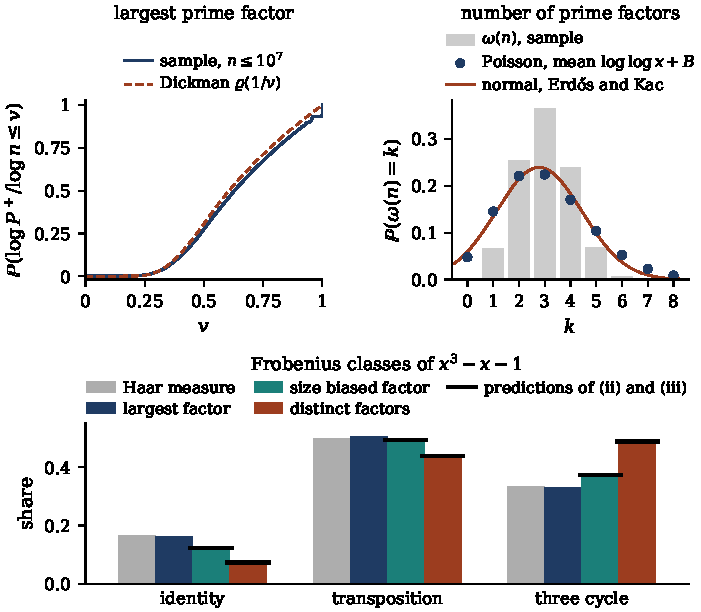
\includegraphics[width=\textwidth]{figs/pd_integers.pdf}
\caption{A sample of $400000$ uniform random integers below $10^7$. Top left: the empirical distribution function of $\log P^+/\log n$ against Dickman's $\varrho(1/v)$ (Theorem~\ref{thm:pdbillingsley}). Top right: the histogram of the number $\omega(n)$ of distinct prime factors, whose mean is close to $\log\log x+B$, with the Poisson law of mean $\log\log x+B$ and the normal law of Erd\H{o}s and Kac, of mean and variance $\log\log x$, neither of which fits at this $x$ (Theorem~\ref{thm:pderdoskac}). Bottom: three colourings of the prime factors by their Frobenius class in the $S_3$ field of $x^3-x-1$ (the class of the largest factor, of a size biased factor, and of the distinct factors pooled over the sample), against Haar measure; the short bars are the predictions of Theorem~\ref{thm:pdmertens}(ii) and (iii) with the constants of Table~\ref{tab:pdmertens}.}\label{fig:pdintegers}
\end{figure}

\section{The Dirichlet process of a random integer}\label{sec:pddirichlet}

Ferguson's Dirichlet process with base measure $\vartheta\mu$, for $\vartheta>0$ and a probability measure $\mu$ on a compact metric space $Y$, is the random probability measure $P=\Gamma_{\vartheta\mu}/\Gamma_{\vartheta\mu}(Y)$ obtained by normalising the Gamma random measure with shape measure $\vartheta\mu$ (\cite{ferguson1973}, Section~4); for every partition $B_1,\dots,B_k$ of $Y$ the vector $(P(B_1),\dots,P(B_k))$ has the Dirichlet law with parameters $(\vartheta\mu(B_1),\dots,\vartheta\mu(B_k))$, and $P$ is independent of the total mass $\Gamma_{\vartheta\mu}(Y)$, which is Gamma with shape $\vartheta$ (\cite{jamesroynetteyor2008}, Section~1.4; \cite{pitman2006}, Section~4.2). Written as $P=\sum_iV_i\delta_{y_i}$ with $V_1\ge V_2\ge\dots$, its weights have the law $\mathrm{PD}(\vartheta)$ and its labels $y_i$ are independent of the weights and of one another, with law $\mu$ (several labels coincide when $\mu$ has atoms); $\mathrm{PD}(1)$ is the case $\vartheta=1$ of Section~\ref{sec:pdlaw}.

Let $N_\sigma$ be the zeta random integer of Chapter~\ref{ch:recip}, $\Prob(N_\sigma=n)=n^{-\sigma}/\zeta(\sigma)$, with prime exponents $e_p$, and let $(\theta_p)$ be labels in $Y$, equidistributed with respect to $\mu$ outside a finite set $S$ of primes. The labelled factorisation is the random measure
\[
\Xi_\sigma=\sum_{p\notin S}(\sigma-1)e_p\log p\;\delta_{\theta_p},
\]
and Theorem~\ref{thm:recipgammaproc} says that $\Xi_\sigma$ converges in law to the Gamma random measure $\Gamma_\mu$ as $\sigma\downarrow1$.

\begin{theorem}[Chebotarev as a Dirichlet process; after \cite{ferguson1973,cifarelliregazzini1990}]\label{thm:pddirichlet}
As $\sigma\downarrow1$:
\begin{enumerate}
\item[(i)] the normalised labelled factorisation $\mathcal P_\sigma=\Xi_\sigma/\Xi_\sigma(Y)$, set equal to $\mu$ on the event $A_\sigma$ that $N_\sigma$ has no prime factor outside $S$, converges in law, as a random probability measure on $Y$ with the weak topology, to the Dirichlet process $P$ with base measure $\mu$, and jointly with it the total mass $\Xi_\sigma(Y)=(\sigma-1)\sum_{p\notin S}e_p\log p$ converges to a standard exponential variable $E$ independent of $P$;
\item[(ii)] for every continuous $Q\ge0$ on $Y$ the Frobenius functional $\Xi_\sigma(Q)$ converges in law to $E\int_YQ\,dP$, a standard exponential variable times a Dirichlet mean, and
\begin{align*}
\E\exp\Bigl(-\lambda\,E\!\int_YQ\,dP\Bigr)&=\E\Bigl(1+\lambda\!\int_YQ\,dP\Bigr)^{-1}\\
&=\exp\Bigl(-\int_Y\log(1+\lambda Q)\,d\mu\Bigr);
\end{align*}
\item[(iii)] for a partition of $Y$ into $\mu$ continuity sets $B_1,\dots,B_k$ with $\mu(B_i)>0$, the shares $\mathcal P_\sigma(B_i)$ converge jointly in law to the Dirichlet law with parameters $\mu(B_i)$, so that each share $\mathcal P_\sigma(B)$ converges to a Beta variable with parameters $(\mu(B),1-\mu(B))$, of mean $\mu(B)$.
\end{enumerate}
\end{theorem}

\begin{proof}
(i) The map $\xi\mapsto(\xi/\xi(Y),\xi(Y))$ is continuous, in the weak topology, at every finite measure with $\xi(Y)>0$, a set of full $\Gamma_\mu$ probability, so the continuous mapping theorem and Theorem~\ref{thm:recipgammaproc}(ii) give convergence of $(\mathcal P_\sigma,\Xi_\sigma(Y))$ to $(\Gamma_\mu/\Gamma_\mu(Y),\Gamma_\mu(Y))$, which is Ferguson's construction of the Dirichlet process with base measure $\mu$, independent of the Gamma total mass of shape $\mu(Y)=1$. (ii) $\Xi_\sigma(Q)=\Xi_\sigma(Y)\int Q\,d\mathcal P_\sigma$ converges by (i) to $E\int Q\,dP$. The first equality is the Gamma integral $\E e^{-\lambda Em}=(1+\lambda m)^{-1}$, conditioned on $\int Q\,dP=m$ and using independence; the second is Theorem~\ref{thm:recipggcfun}, since $\Xi_\sigma(Q)$ converges in law to the GGC whose Laplace transform is the right hand side. (iii) follows from (i): $\E P(\partial B_i)=\mu(\partial B_i)=0$, so $\nu\mapsto(\nu(B_1),\dots,\nu(B_k))$ is continuous at almost every $P$, and the shares of a Dirichlet process are Dirichlet.
\end{proof}

For Frobenius classes in a finite Galois group $G$, with $\mu$ the image of Haar measure on the set of classes, Chebotarev's theorem supplies the hypothesis, and the proof of Lemma~\ref{lem:recipnu} uses only its Dirichlet density form $\sum_{p\in C}(\log p)p^{-s}\sim\delta(C)/(s-1)$ as $s\downarrow1$, with $\delta(C)=|C|/|G|$. Then (i) and (iii) are Corollary~\ref{cor:recipchebgamma}(ii) of Chapter~\ref{ch:recip} read as a statement about the Dirichlet process: the share $\mathcal P_\sigma(C)$ carried by the primes with Frobenius in a class $C$ is asymptotically $\mathrm{Beta}(\delta(C),1-\delta(C))$, with mean Chebotarev's density $\delta(C)$.

The identity between the last two expressions in (ii), $\E(1+\lambda\int Q\,dP)^{-\vartheta}=\exp(-\vartheta\int\log(1+\lambda Q)\,d\mu)$ for a Dirichlet process with base measure $\vartheta\mu$, is Cifarelli and Regazzini's identity for Dirichlet means \cite{cifarelliregazzini1990}, the Markov Krein identity when $\vartheta=1$ (Diaconis and Kemperman \cite{diaconiskemperman1996}), in the form of James, Roynette and Yor (\cite{jamesroynetteyor2008}, Section~1.4, (33)): a GGC of finite Thorin mass is a Gamma variable times an independent Dirichlet mean, whose atomic case, Theorem~\ref{thm:lapspline}, writes atomic Thorin laws as Gamma variables times B spline variables. Here it says what the Thorin measure of a Frobenius functional is: the limit of $\Xi_\sigma(Q)$ is a GGC with Thorin mass $\mu(Q>0)$ and Thorin measure the image of $\mu$ restricted to $\{Q>0\}$ under $1/Q$ (Theorem~\ref{thm:recipggcfun}), and it is also a Gamma variable of shape $\mu(Q>0)$ times the Dirichlet mean $\int Q\,dP'$ of an independent Dirichlet process $P'$ with base measure $\mu$ restricted to $\{Q>0\}$. Figure~\ref{fig:pddirichlet}, left, checks the identity in the simplest case, $Q=\operatorname{tr}^2$ for the two dimensional representation of $S_3$ (traces $2,0,-1$ on the three classes) with Haar measure, where $\int Q\,dP=4P(\{1\})+P(C_3)$, with $\{1\}$, $C_2$ and $C_3$ the identity, the transpositions and the three cycles, and $(P(\{1\}),P(C_2),P(C_3))$ Dirichlet with parameters $(\frac16,\frac12,\frac13)$: two million samples of $E(4P(\{1\})+P(C_3))$ reproduce $\exp(-\frac16\log(1+4\lambda)-\frac13\log(1+\lambda))$ to $2.8\cdot10^{-4}$. The Laplace transform at $\sigma=1.01$, computed from the Euler product over the primes below $10^7$, with the prime number theorem for the larger primes, lies $0.036$ above the limit at $\lambda=6$; this is the Euler Kronecker drift of Theorem~\ref{thm:recipdrift}, of order $\sigma-1$ (its first order term $\kappa_Q\lambda(\sigma-1)$, with $\kappa_Q=\sum_CQ_C\kappa_C=2.53$ for $S=\{23\}$, is $0.15$ in the logarithm, against the observed $0.11$, the identity class being evaluated at $\sigma+24(\sigma-1)=1.25$), not a defect of the identity.

\begin{figure}[!htbp]
\centering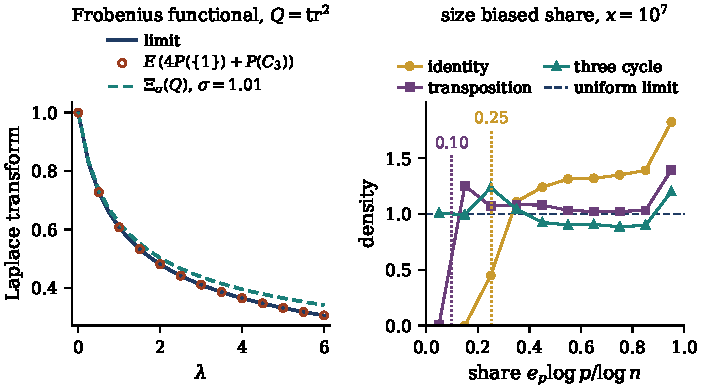
\includegraphics[width=\textwidth]{figs/pd_dirichlet.pdf}
\caption{Left: Theorem~\ref{thm:pddirichlet}(ii) for $Q=\operatorname{tr}^2$, the squared trace of the two dimensional representation of the $S_3$ field of $x^3-x-1$: the Laplace transform of the limit, $\exp(-\frac16\log(1+4\lambda)-\frac13\log(1+\lambda))$, that of two million samples of $E(4P(\{1\})+P(C_3))$, a standard exponential variable times a Dirichlet mean, and that of $\Xi_\sigma(Q)$ at $\sigma=1.01$ (primes below $10^7$, prime number theorem beyond). Right: the size biased share $e_p\log p/\log n$ of the $400000$ uniform random integers below $10^7$ of Figure~\ref{fig:pdintegers}, by Frobenius class of the chosen prime $p$. The limit is uniform for every class (Theorem~\ref{thm:pdsizebiased}); at $x=10^7$ the share is at least $\log59/\log10^7=0.25$ when $p$ is in the identity class, whose smallest prime is $59$, and at least $\log5/\log10^7=0.10$ when $p$ is in the class of transpositions, whose smallest prime is $5$ (both floors marked). The rise in the last bin is the atom at share $1$ of the prime powers $n=p^k$, nearly all of them primes.}\label{fig:pddirichlet}
\end{figure}

Theorem~\ref{thm:pddirichlet} has two readings. The first is Bayesian: in Chapter~\ref{ch:12} the Dirichlet process is a nonparametric prior on the trace law, set aside there because its draws are discrete; here it is the limit law of the labelled factorisation, with the equidistribution measure (Haar measure for Frobenius classes) as base measure, and Ferguson's conjugacy (\cite{ferguson1973}, Section~3, Theorem~1), which turns a prior with base measure $\vartheta\mu$ into a posterior with base measure $\vartheta\mu+\sum_i\delta_{y_i}$ after labels $y_1,\dots,y_n$, applies to it unchanged. The second is the Chinese restaurant process. Sampling points from a Dirichlet process with base measure $\vartheta\mu$ produces, by the P\'olya urn of Blackwell and MacQueen \cite{blackwellmacqueen1973}, a random partition: the $n$th point joins an existing cluster of size $m$ with probability $m/(n-1+\vartheta)$ and opens a new cluster, with a fresh label drawn from $\mu$, with probability $\vartheta/(n-1+\vartheta)$. The cluster sizes follow the Ewens sampling formula with parameter $\vartheta$ \cite{ewens1972,antoniak1974,hoppe1984}, and the cluster labels are independent with law $\mu$. For $\vartheta=1$ the partition of $n$ sampled points has the law of the cycle type of a uniform permutation of $n$ letters, which is the sense in which the large prime factors of a random integer and the long cycles of a random permutation have the same limit.

\section{The Ewens family from the coefficients of \texorpdfstring{$\zeta^\vartheta$}{zeta to the theta}}\label{sec:pdtheta}

The zeta subordinator $X_t$ of Chapter~\ref{ch:10d} runs, by Proposition~\ref{prop:10dsublaw}, through the random integers whose law is $d_t(n)n^{-\sigma}/\zeta(\sigma)^t$, where $d_t$ are the Dirichlet coefficients of $\zeta^t$, multiplicative with $d_t(p^k)=\binom{t+k-1}k$. For $t=1$ this is $N_\sigma$; for $t=2$ the weight is the divisor function. These integers, with $t=\vartheta$, give the whole Ewens family.

\begin{theorem}[the prime factors of the $\zeta^\vartheta$ random integer are Poisson Dirichlet with parameter $\vartheta$; after \cite{elboimgorodetsky2024,sun2026}]\label{thm:pdtheta}
Fix $\vartheta>0$ and let the random integer $N_\sigma^{(\vartheta)}$ have the law $d_\vartheta(n)n^{-\sigma}/\zeta(\sigma)^\vartheta$, with labels $(\theta_p)$ equidistributed with respect to $\mu$ outside $S$, and let $\Xi^{(\vartheta)}_\sigma=\sum_{p\notin S}(\sigma-1)e_p\log p\,\delta_{\theta_p}$ be its labelled factorisation. Then the prime exponents are independent negative binomial variables, $\Prob(e_p=k)=\binom{\vartheta+k-1}k(1-p^{-\sigma})^\vartheta p^{-k\sigma}$, and as $\sigma\downarrow1$:
\begin{enumerate}
\item[(i)] the marked process $\sum_{p\notin S,\,e_p\ge1}\delta_{((\sigma-1)e_p\log p,\,\theta_p)}$ converges in law, vaguely on $(0,\infty)\times Y$, to the Poisson process with intensity $\vartheta x^{-1}e^{-x}dx\otimes\mu$;
\item[(ii)] the labelled factorisation $\Xi^{(\vartheta)}_\sigma$ converges in law to the Gamma random measure with shape measure $\vartheta\mu$, its total mass, which is $(\sigma-1)\log N^{(\vartheta)}_\sigma$ up to the primes in $S$, to a Gamma variable with shape $\vartheta$, and the normalised factorisation to the Dirichlet process with base measure $\vartheta\mu$;
\item[(iii)] the ranked normalised sizes of the prime factors converge to $\mathrm{PD}(\vartheta)$, and for every continuous $Q\ge0$ the functional $\Xi^{(\vartheta)}_\sigma(Q)$ converges to a GGC with Thorin measure $\vartheta$ times the image of $\mu|_{\{Q>0\}}$ under $1/Q$.
\end{enumerate}
\end{theorem}

\begin{proof}
The generating function of the law is $\zeta(\sigma)^{-\vartheta}\sum_nd_\vartheta(n)n^{-\sigma}\prod_pt_p^{e_p}=\prod_p\bigl((1-p^{-\sigma})/(1-t_pp^{-\sigma})\bigr)^\vartheta$, a product over primes, so the exponents are independent and negative binomial. It is the $\vartheta$th power of the generating function of $N_\sigma$ (Lemma~\ref{lem:recipzeta}), so $\E e^{-\Xi^{(\vartheta)}_\sigma(\lambda)}=(\E e^{-\Xi_\sigma(\lambda)})^\vartheta$ for continuous $\lambda\ge0$, and Theorem~\ref{thm:recipgammaproc}(ii) gives the first two parts of (ii). The proof of Theorem~\ref{thm:recipgammaproc}(i) gives (i), with $\Prob(e_p=k)\le\binom{\vartheta+k-1}kp^{-k}$, whose sum over $k\ge2$ is $O(p^{-2})$, in place of $p^{-k}$, and $\vartheta p^{-\sigma}$ in place of $p^{-\sigma}$. The atoms of size below $a$ carry expected mass at most $\vartheta\nu_\sigma([0,a)\times Y)+O(\sigma-1)$, with $\nu_\sigma$ as in Lemma~\ref{lem:recipnu}, which tends to $\vartheta(1-e^{-a})$, uniformly small as $a\to0$; so the total mass converges jointly with the marked process of (i), and the ranked sizes divided by the total converge to the ranked jumps of a Gamma subordinator on $[0,\vartheta]$ divided by their sum, which is $\mathrm{PD}(\vartheta)$ \cite{kingman1975}. The third part of (ii) follows as in Theorem~\ref{thm:pddirichlet}, with $\Gamma_{\vartheta\mu}(Y)$ Gamma of shape $\vartheta$, and the GGC limit in (iii) is (ii) applied to $\lambda Q$, as in the proof of Theorem~\ref{thm:recipggcfun}.
\end{proof}

So the parameter of the Poisson Dirichlet law is the exponent $\vartheta$ of the singularity $(s-1)^{-\vartheta}$ of the generating Dirichlet series at $s=1$, the order of a pole when $\vartheta$ is an integer. For the Rankin Selberg random integer of an Artin representation $\rho$, with law proportional to the coefficients, which are nonnegative, of $L^S(s,\rho\otimes\check\rho)$, the $L$ function without its Euler factors at the ramified primes, the exponents are $e_p=\sum_mmM(p^m)$ with independent Poisson variables $M(p^m)$ of means $|\chi_\rho(\Frob_p^m)|^2p^{-m\sigma}/m$, and Theorem~\ref{thm:pdewens} below gives a marked limit with intensity $x^{-1}e^{-x}dx\otimes|\chi_\rho|^2\mu$, of total mass $\langle\rho,\rho\rangle$. So the Gamma shape of Theorem~\ref{thm:recipgamma} is an Ewens parameter, the normalised factorisation converges to the Dirichlet process with base measure $|\chi_\rho|^2\mu$ rather than a multiple of Haar measure, and the ranked sizes are $\mathrm{PD}(\langle\rho,\rho\rangle)$: $\mathrm{PD}(1)$ for irreducible $\rho$ and $\mathrm{PD}(4)$ for $\rho\oplus\rho$, with correspondingly more and smaller prime factors.

\section{Three colourings and their rates}\label{sec:pdmertens}

Theorem~\ref{thm:pddirichlet} is a statement about the zeta random integer as $\sigma\downarrow1$. For a uniform random integer below $x$ the sizes have the same limit (Theorem~\ref{thm:pdbillingsley}), but the rates differ sharply between three natural ways of colouring the prime factors by their Frobenius classes, and the differences are visible at $x=10^7$. Let $K/\Q$ be Galois with group $G$, $C\subset G$ a conjugacy class with Haar measure $\delta(C)=|C|/|G|$, which is $\mu(C)$ in the notation of Chapter~\ref{ch:recip}, and write $p\in C$ when the Frobenius class of $p$ is $C$. The three colourings of $n$ are: the class of the largest prime factor $P^+(n)$; the class of a \emph{size biased} prime factor, chosen with probability $e_p\log p/\log n$; and the classes of the distinct prime factors, pooled over $n$, that is the ratio $\E\omega_C(n)/\sum_{C'}\E\omega_{C'}(n)$, where $\omega_C(n)$ counts the distinct prime factors of $n$ in $C$.

\begin{theorem}[three colourings; (i) Dawsey \cite{dawsey2017}, (ii) this book, (iii) Mertens per class \cite{bardestanifreiberg2013}]\label{thm:pdmertens}
Let $n$ be uniform on $\{2,\dots,x\}$, and let the ramified primes be left out of every class. By the prime number theorem for $K$ in the form \cite{lagariasodlyzko1977}
\[
\pi_C(t)=\delta(C)\operatorname{li}(t)+O\bigl(t\exp(-a_K\sqrt{\log t})\bigr),
\]
the limits
\begin{align*}
b_C&=\lim_{t\to\infty}\Bigl(\sum_{p\le t,\,p\in C}\frac1p-\delta(C)\log\log t\Bigr),\\
c_C&=\lim_{t\to\infty}\Bigl(\sum_{p\le t,\,p\in C}\frac{\log p}p-\delta(C)\log t\Bigr)
\end{align*}
exist, with $\sum_Cb_C=B-\sum_{p\text{ ram.}}1/p$ and $\sum_Cc_C=c-\sum_{p\text{ ram.}}\log p/p$, where $B=0.26150$ and $c=-\gamma_{\mathrm E}-\sum_p\log p/(p(p-1))=-1.33258$ are the two Mertens constants. Let $\kappa_C=-c_C-\sum_{p\in C}\log p/(p(p-1))$, which by the Abelian theorem is the Euler Kronecker drift of Theorem~\ref{thm:recipdrift} for $S$ the set of ramified primes, so that $\sum_C(\gamma_{\mathrm E}\delta(C)-\kappa_C)=-\sum_{p\text{ ram.}}\log p/(p-1)$. Then, as $x\to\infty$:
\begin{enumerate}
\item[(i)] $\Prob(P^+(n)\in C)=\delta(C)+O\bigl(\exp(-a_K'(\log x)^{1/3})\bigr)$ for some $a_K'>0$;
\item[(ii)] the size biased prime factor lies in $C$ with probability
\[
\delta(C)+\frac{\gamma_{\mathrm E}\delta(C)-\kappa_C}{\log x-1}+O\bigl((\log x)^{-2}\bigr);
\]
\item[(iii)] $\E\,\omega_C(n)=\delta(C)\log\log x+b_C+O(1/\log x)$, so that with $B'=B-\sum_{p\text{ ram.}}1/p$ the ratio of means $\E\omega_C(n)/\sum_{C'}\E\omega_{C'}(n)$, the share of the unramified distinct prime factors that lie in $C$, equals
\[
\delta(C)+\frac{b_C-\delta(C)B'}{\log\log x+B'}+O\Bigl(\frac1{\log x\,\log\log x}\Bigr).
\]
\end{enumerate}
\end{theorem}

\begin{proof}
The constants exist by partial summation against $\pi_C(t)-\delta(C)\operatorname{li}(t)$, exactly as in Mertens's theorems for $\pi(t)$ \cite{mertens1874,tenenbaum2015}; the sums over all classes are the classical constants. (i) is Dawsey's theorem (\cite{dawsey2017}, Theorem~2), which extends Alladi's for progressions \cite{alladi1977}. The error is so small because the unlabelled count is exact: every $n$ with $2\le n\le x$ is $pm$ with $p=P^+(n)$ and $m\le x/p$ free of primes above $p$, so $\sum_{p\le x}\Psi(x/p,p)=\lfloor x\rfloor-1$, with $\Psi(y,p)$ the number of such $m\le y$, and only the equidistribution of the primes of $C$, weighted by $\Psi(x/p,p)$, enters. (iii) By Mertens's theorem for the class (\cite{bardestanifreiberg2013}, Theorems~8.3 and 8.5),
\begin{align*}
\E\omega_C(n)&=\frac1{\lfloor x\rfloor-1}\sum_{p\le x,\,p\in C}\Bigl\lfloor\frac xp\Bigr\rfloor=\sum_{p\le x,\,p\in C}\frac1p+O\Bigl(\frac1{\log x}\Bigr)\\
&=\delta(C)\log\log x+b_C+O\Bigl(\frac1{\log x}\Bigr);
\end{align*}
summing over the classes gives $\log\log x+B'+O(1/\log x)$, and the ratio of the two expansions is the display. (ii) Write $\ell_C(n)=\sum_{p\in C}e_p\log p$, so that the size biased factor lies in $C$ with probability $\E[\ell_C(n)/\log n]$. Replacing $1/\log n$ by $1/(\log x-1)$, where $\log x-1+O(\log x/x)$ is the mean of $\log n$, costs $O((\log x)^{-2})$: for $n\ge\sqrt x$, writing $u=\log(n/x)$,
\[
\frac1{\log n}=\frac1{\log x-1}-\frac{u+1}{(\log x-1)^2}+O\Bigl(\frac{(u+1)^2}{(\log x)^3}\Bigr);
\]
the first order term is handled by $\E[\ell_C(n)(u+1)]=O(1)$, because for each prime power $y=x/p^k$ the inner sum $\sum_{m\le y}(\log(m/y)+1)$ is $O(\log y+1)$, the second by $\E[\ell_C(n)(u+1)^2]\le\log x\,\E(u+1)^2=O(\log x)$, and the $n<\sqrt x$ have probability $O(x^{-1/2})$. Now $(\lfloor x\rfloor-1)\E e_p=\sum_{k\ge1}\lfloor x/p^k\rfloor=x/(p-1)-\sum_{k\ge1}\{x/p^k\}$. Summing over $p\le x$ in $C$, with $x/(\lfloor x\rfloor-1)=1+O(1/x)$, the main term is
\[
\sum_{p\le x,\,p\in C}\frac{\log p}{p-1}=\delta(C)\log x+c_C+\sum_{p\in C}\frac{\log p}{p(p-1)}+O\Bigl(\frac1{\log x}\Bigr)
\]
by the definition of $c_C$, and the fractional parts contribute
\[
-\frac1x\sum_{p\le x,\,p\in C}\log p\,\Bigl\{\frac xp\Bigr\}+O\Bigl(\frac1{\log x}\Bigr)=-\delta(C)(1-\gamma_{\mathrm E})+O\Bigl(\frac1{\log x}\Bigr).
\]
The last estimate is the class version of
\[
\sum_{n\le x}\Lambda(n)\Bigl\{\frac xn\Bigr\}=(1-\gamma_{\mathrm E})x+O\Bigl(\frac x{\log x}\Bigr),
\]
which follows from $\log\lfloor x\rfloor!=\sum_{n\le x}\Lambda(n)\lfloor x/n\rfloor$ and $\sum_{n\le x}\Lambda(n)/n=\log x-\gamma_{\mathrm E}+o(1/\log x)$: on each interval $x/(j+1)<p\le x/j$ with $j<\log x$ the function $\{x/p\}=x/p-j$ is monotone, and partial summation against $\sum_{p\le t,\,p\in C}\log p-\delta(C)\sum_{p\le t}\log p=O(t\exp(-a_K\sqrt{\log t}))$ replaces the sum over $p\in C$ by $\delta(C)$ times the sum over all primes, with an error $O(x/\log x)$, the primes $p\le x/\log x$ contributing $O(x/\log x)$. This term $-\delta(C)(1-\gamma_{\mathrm E})$ is why the constant carries the term $\gamma_{\mathrm E}\delta(C)$. Hence $\E\ell_C(n)=\delta(C)(\log x-1)+\gamma_{\mathrm E}\delta(C)-\kappa_C+O(1/\log x)$, and dividing by $\log x-1$ gives (ii).
\end{proof}

For the zeta integer the same constant is, by Theorem~\ref{thm:recipdrift}, the first order term of the ratio of means $\E L_C(\sigma)/\E[(\sigma-1)\log N_\sigma]=\delta(C)+(\gamma_{\mathrm E}\delta(C)-\kappa_C)(\sigma-1)+O((\sigma-1)^2)$, with $L_C(\sigma)$ the rescaled class mass of Corollary~\ref{cor:recipchebgamma} and $\sigma-1$ in the place of $1/(\log x-1)$.

\begin{table}[!htbp]
\centering\small
\begin{tabular}{@{}lccccc@{}}
\toprule
class $C$ of $x^3-x-1$ & $\delta(C)$ & $b_C$ & $c_C$ & $\gamma_{\mathrm E}\delta(C)-\kappa_C$ & smallest prime\\
\midrule
identity ($3$ roots) & $1/6$ & $-0.2436$ & $-0.7429$ & $-0.6439$ & $59$\\
transposition ($1$ root) & $1/2$ & $-0.0755$ & $-0.5931$ & $-0.1211$ & $5$\\
three cycle ($0$ roots) & $1/3$ & $0.5372$ & $-0.1327$ & $0.6226$ & $2$\\
\bottomrule
\end{tabular}
\caption{Mertens constants per Frobenius class, computed from the unramified primes below $10^7$, for the $S_3$ extension of $x^3-x-1$; the ramified prime $23$ is left out, so the $b_C$ sum to $0.2180=B-\frac1{23}$ and the $c_C$ to $-1.4687$, against the limit $c-\frac{\log23}{23}=-1.4689$. The identity class has a large negative $b_C$ because its first prime is $59$; the three cycle class, which contains $2$, $3$ and $13$, has a large positive one.}\label{tab:pdmertens}
\end{table}

Table~\ref{tab:pdmertens} gives the constants for the running example, and Figure~\ref{fig:pdintegers}, bottom, compares the three colourings at $x=10^7$ with Haar measure and with the predictions of the theorem. The largest prime factor is already close to Haar: shares $0.161$, $0.506$, $0.332$ against $\frac16,\frac12,\frac13$, the deviation at this $x$ coming from the small primes. For the zeta integer this is Theorem~\ref{thm:hitrate}(ii), and Chapter~\ref{ch:hit} computes its approach, linear in $\sigma-1$, for the same field. The size biased factor has shares $0.124$, $0.492$, $0.374$, against the prediction $0.124$, $0.492$, $0.375$ of (ii), and the remaining $0.93$ percent of picks fall on the ramified prime $23$, against $\log23/(22(\log x-1))$, that is $0.94$ percent. The distinct prime factors, pooled over all $400000$ integers, have shares $0.072$, $0.438$, $0.489$, against the prediction $0.073$, $0.438$, $0.488$ of (iii), and the identity class is at less than half its Haar measure. The reason is in the last column of the table: the count of distinct prime factors is dominated by small primes, whose classes are fixed, and the identity class has no prime below $59$. The deficit of its share, $(b_C-\delta(C)B')/(\log\log x+B')$ with $b_C-\delta(C)B'=-0.280$, decays only like $1/\log\log x$: it is $-0.093$ at $x=10^7$ and still $-0.059$ at $x=10^{40}$. Chebotarev's theorem holds for all three colourings, but for the third the identity class is still more than a third below its Haar measure at $x=10^{40}$. The same effect sits inside Theorem~\ref{thm:pdsizebiased} below: the Frobenius class and the size of a size biased factor are asymptotically independent, but at $x=10^7$ a size biased factor in the identity class carries at least $\log59/\log10^7=0.25$ of $\log n$ (Figure~\ref{fig:pddirichlet}, right). So the statistics of a random integer that see Chebotarev's theorem at a computable scale are those that select or weight prime factors by their size, as the Frobenius functionals of Chapter~\ref{ch:recip} do with the weight $e_p\log p$; counting distinct prime factors, where the small primes dominate, does not.

\begin{theorem}[size biased factors are uniform, whatever their class; after Donnelly and Grimmett \cite{donnellygrimmett1993}]\label{thm:pdsizebiased}
Let $n$ be uniform on $\{2,\dots,x\}$, let $p^*$ be a size biased prime factor of $n$, and let $F^*=e_{p^*}\log p^*/\log n$ be its share. As $x\to\infty$, $p^*$ is unramified with probability tending to $1$, and $(F^*,\text{class of }p^*)$ converges in law to the product of the uniform law on $(0,1)$ and the law $C\mapsto\delta(C)$ on the classes. The same holds for the zeta random integer as $\sigma\downarrow1$, with $p^*$ picked, off $A_\sigma$, among the prime factors outside $S$ and its share taken relative to their part of $\log N_\sigma$.
\end{theorem}

\begin{proof}
For the uniform integer the statement is a first moment computation:
\[
\Prob(p^*\in C,\ F^*\le f)=\E\sum_{p\in C}\frac{e_p\log p}{\log n}\mathsf1\{e_p\log p\le f\log n\}.
\]
The terms with $e_p\ge2$ contribute $O(1/\log x)$, the integers $n\le x/(\log x)^2$ contribute $O((\log x)^{-2})$, and for the others $\log n=\log x+O(\log\log x)$, so the probability is $(\log x)^{-1}\sum_{p\le x^f,\,p\in C}\log p/p+O(\log\log x/\log x)=\delta(C)f+o(1)$ by Mertens's first theorem for the class, which follows from the existence of $c_C$ in Theorem~\ref{thm:pdmertens}. For the zeta integer, the proof of Theorem~\ref{thm:pdtheta} with $\vartheta=1$ shows that the rescaled sizes with their labels and the total mass converge jointly, so that the normalised sizes converge to $\mathrm{PD}(1)$, a limit that goes back to Lloyd \cite{lloyd1984}, with labels independent of the sizes and of law $\mu$ (Theorem~\ref{thm:recipgammaproc}(i)). Since picking in proportion to size is a continuous operation outside a null set, the share of $p^*$ converges to a size biased pick from $\mathrm{PD}(1)$, which is uniform (\cite{pitman2006}, Section~3.1), and its class to an independent label of law $\mu$.
\end{proof}

\section[Mertens constants, empty classes and Ewens parameters]{Mertens constants, empty classes\\ and Ewens parameters}\label{sec:pdprogress}

This section answers two questions about the limits above and bounds a third from one side. The Mertens constants per class are explicit in $L(1,\chi)$ and $\frac{L'}L(1,\chi)$ (Theorem~\ref{thm:pdmertensL}). The Ewens parameter of an Euler product whose logarithm has nonnegative coefficients, given at the primes by a continuous function of equidistributed labels, is the exponent of its singularity at $s=1$, the order of its pole when it continues meromorphically, and the colouring of its random integer is the equidistribution measure weighted by that function (Theorem~\ref{thm:pdewens}). And while the Euler Kronecker drifts of Chapter~\ref{ch:recip} govern the means, the Kolmogorov distance between the law of the share of a class $C$ and its Beta limit is at least of order $(\sigma-1)^{\delta(C)}$, because at any $\sigma>1$ the class is empty with probability of that order, which Chapter~\ref{ch:recip} found (Theorem~\ref{thm:recipggcfun} and the paragraph after it) and Theorem~\ref{thm:pdrate} gives with its constant. The constants of the first and last answers come from one function, the regular part $h_C$ of the partial Euler product over a class: $b_C$ and the constant of the last answer from its value at $s=1$, and $c_C$ from its derivative there.

Throughout, $K/\Q$ is Galois with group $G$, $S$ is the set of ramified primes and $C$ a class with $\delta(C)=|C|/|G|$. As in the proof of Theorem~\ref{thm:recipdrift},
\[
P_C(s)=\sum_{p\notin S,\ \Frob_p\in C}\ \sum_{m\ge1}\frac{p^{-ms}}m=\sum_\chi c_\chi\log L^S(s,\chi)+R_C(s),
\]
with $c_\chi=\delta(C)\overline{\chi(C)}$ for each irreducible character $\chi$, $L^S$ the $L$ function without its Euler factors at $S$, and a prime power term $R_C$ holomorphic on $\operatorname{Re}s>\frac12$. By Brauer's theorem and the nonvanishing of Artin $L$ functions at $s=1$, $h_C(s)=P_C(s)-\delta(C)\log\frac1{s-1}$ is real analytic near $s=1$, and $h_C'(1)$ is the drift $\kappa_C$ of that theorem for this $S$.

\subsection{Mertens constants from \texorpdfstring{$L(1,\chi)$}{L(1,chi)}}

\begin{theorem}[Mertens constants per class; after \cite{williams1974,bardestanifreiberg2013}]\label{thm:pdmertensL}
With $b_C$ and $c_C$ as in Theorem~\ref{thm:pdmertens} and $B$, $c$ the Mertens constants,
\begin{align*}
b_C&=\delta(C)\Bigl(B-\sum_{p\in S}\frac1p\Bigr)+\sum_{\chi\ne1}c_\chi\Bigl[\log L^S(1,\chi)-\sum_{p\notin S}\sum_{m\ge2}\frac{\chi(\Frob_p^m)}{m\,p^m}\Bigr],\\
c_C&=\delta(C)\Bigl(c-\sum_{p\in S}\frac{\log p}p\Bigr)-\sum_{\chi\ne1}c_\chi\Bigl[\frac{(L^S)'}{L^S}(1,\chi)+\sum_{p\notin S}\sum_{m\ge2}\frac{\chi(\Frob_p^m)\log p}{p^m}\Bigr],
\end{align*}
and the constant term of $P_C$ at $s=1$ is
\[
h_C(1)=b_C-\gamma_{\mathrm E}\,\delta(C)+\sum_{p\notin S,\,\Frob_p\in C}\ \sum_{m\ge2}\frac{p^{-m}}m .
\]
\end{theorem}

\begin{proof}
Expand $\mathsf1_C(\Frob_p)=\sum_\chi c_\chi\chi(\Frob_p)$. The term $\chi=1$ gives, by Mertens, $\delta(C)$ times $\sum_{p\le t,\,p\notin S}1/p$, which is $\log\log t+B-\sum_{p\in S}1/p+o(1)$. For $\chi\ne1$ the partial sums $\sum_{p\le t,\,p\notin S}\chi(\Frob_p)/p$ converge to the bracket in the theorem: the Dirichlet series $\sum_{p\notin S}\chi(\Frob_p)p^{-s}$ equals $\log L^S(s,\chi)$ minus the prime power sum, which is holomorphic on $\operatorname{Re}s>\frac12$, and $L^S(s,\chi)$ is holomorphic and nonzero on $\operatorname{Re}s\ge1$, so the partial sums converge to the value at $s=1$ by the prime number theorem for $K$ and partial summation, exactly as for Dirichlet characters \cite{tenenbaum2015}; for Chebotarev classes see \cite{bardestanifreiberg2013}, Theorem~8.3. The formula for $c_C$ is the same argument with $\log p/p$ in place of $1/p$, the $\chi=1$ term being the prime number theorem in the form $\sum_{p\le t}\log p/p=\log t+c+o(1)$ and the others the derivative of $-\log L^S(s,\chi)$ at $1$. For $h_C(1)$, the Abelian theorem $\sum_{p\in C}p^{-s}=\delta(C)\log\frac1{s-1}+b_C-\gamma_{\mathrm E}\delta(C)+o(1)$ follows from $\sum_{p\le t,\,p\in C}1/p=\delta(C)\log\log t+b_C+o(1)$ by partial summation, and the prime powers add their convergent sum.
\end{proof}

The formula for $c_C$ is Theorem~\ref{thm:recipdrift} in other terms: by the Abelian theorem $c_C+\sum_{p\in C}\log p/(p(p-1))=-\kappa_C$, minus the drift of the class $C$. The formula for $b_C$, its analogue for the weights $1/p$ with $\log L(1,\chi)$ in place of $\frac{L'}L(1,\chi)$, is (8.1), (8.2) and Theorem~8.3 of Bardestani and Freiberg \cite{bardestanifreiberg2013}, and the asymptotic $\prod_{p\le x,\,p\in C}(1-1/p)\sim e^{-h_C(1)-\gamma_{\mathrm E}\delta(C)}(\log x)^{-\delta(C)}$ is (8.8) of the same theorem, and with an error term Theorem~A of Arango Pi\~neros, Keliher and Keyes \cite{arangopinerokeliherkeyes2022}.

For the $S_3$ field of $x^3-x-1$, with $S=\{23\}$, the characters are the trivial one, the sign $\chi_{-23}$ and the two dimensional $\rho$, with $L(1,\chi_{-23})=3\pi/\sqrt{23}=1.965202$, $L^{(23)}(1,\rho)=0.352392$, $\frac{L'}L(1,\chi_{-23})=-0.422121$ and $\frac{(L^{(23)})'}{L^{(23)}}(1,\rho)=1.159587$ from PARI. The theorem gives $b_C=-0.243641$, $-0.075520$, $0.537179$ and $c_C=-0.742978$, $-0.593191$, $-0.132738$ for the identity, the transpositions and the three cycles, against the values $-0.243638$, $-0.075516$, $0.537183$ and $-0.742913$, $-0.593134$, $-0.132674$ read from the primes below $10^7$ in Table~\ref{tab:pdmertens}; the differences, below $7\cdot10^{-5}$, are the tails beyond $10^7$, and with the primes below $10^9$ they fall below $3\cdot10^{-5}$. The constants $h_C(1)$ are $-0.33954$, $-0.32024$ and $0.61533$. What the theorem leaves open is the sign of the deficit of the identity class as the field varies, Open Problem~\ref{op:pdmertens}.

\subsection{Atoms at zero: a class is empty with probability of order \texorpdfstring{$(\sigma-1)^{\delta(C)}$}{(sigma-1) to the delta(C)}}

For $Q=\mathsf1_C$ the probability in Theorem~\ref{thm:recipggcfun} that no prime factor of $N_\sigma$ has a label where $Q>0$ is the probability that the class $C$ is empty, of exact order $(\sigma-1)^{\delta(C)}$ by the paragraph after that theorem. The next theorem gives its constant, and the atom at zero that it describes bounds from below the Kolmogorov distance between the law of a share and its Beta limit.

\begin{theorem}[atoms at zero and a lower bound for the rate; (i) refines Theorem~\ref{thm:recipggcfun}, (iii) after Serre \cite{serre1976}]\label{thm:pdrate}
Let $G$ be nontrivial, let $L_C(\sigma)$ be the mass of the class $C$, as in Corollary~\ref{cor:recipchebgamma}, let $A_\sigma$ be the event that $N_\sigma$ has no prime factor outside $S$, and let $\mathcal P_\sigma(C)$ be the share of $C$, equal to $L_C(\sigma)/\sum_{C'}L_{C'}(\sigma)$ off $A_\sigma$ and to $\delta(C)$ on $A_\sigma$, as in Theorem~\ref{thm:pddirichlet}.
\begin{enumerate}
\item[(i)] $\Prob(L_C(\sigma)=0)=e^{-P_C(\sigma)}=e^{-h_C(1)}(\sigma-1)^{\delta(C)}\bigl(1+O(\sigma-1)\bigr)$, with $h_C(1)$ as in Theorem~\ref{thm:pdmertensL}.
\item[(ii)] The Kolmogorov distance between the law of $\mathcal P_\sigma(C)$ and its limit $\mathrm{Beta}(\delta(C),1-\delta(C))$ is at least
\[
\Prob(L_C(\sigma)=0)-\Prob(A_\sigma)=e^{-h_C(1)}(\sigma-1)^{\delta(C)}\bigl(1+o(1)\bigr),
\]
hence at least of order $(\sigma-1)^{\delta_{\min}}$ for the smallest class, $\delta_{\min}=\min_C\delta(C)$.
\item[(iii)] For the uniform random integer below $x$ the same exponent appears in the density of the integers free of $C$: the proportion of $n\le x$ with no prime factor in $C$ equals $K_C(\log x)^{-\delta(C)}(1+O(1/\log x))$, where
\[
K_C=\frac{e^{\gamma_{\mathrm E}\delta(C)}}{\Gamma(1-\delta(C))}\lim_{t\to\infty}(\log t)^{\delta(C)}\prod_{p\le t,\,p\in C}\Bigl(1-\frac1p\Bigr)=\frac{e^{-h_C(1)}}{\Gamma(1-\delta(C))}:
\]
the same constant $e^{-h_C(1)}$ governs the zeta integer, through $e^{-h_C(1)}(\sigma-1)^{\delta(C)}$, and the uniform integer, through $e^{-h_C(1)}(\log x)^{-\delta(C)}/\Gamma(1-\delta(C))$.
\end{enumerate}
\end{theorem}

\begin{proof}
(i) By Lemma~\ref{lem:recipzeta} the exponents are independent and $\Prob(e_p=0)=1-p^{-\sigma}$, so $\Prob(L_C(\sigma)=0)=\prod_{p\in C}(1-p^{-\sigma})=\exp(-P_C(\sigma))$, and $P_C(\sigma)=\delta(C)\log\frac1{\sigma-1}+h_C(1)+O(\sigma-1)$ by the analyticity of $h_C$. (ii) The Beta law has no atom at $0$, while $\mathcal P_\sigma(C)=0$ exactly when $L_C(\sigma)=0$ and $A_\sigma$ fails, and $A_\sigma\subset\{L_C(\sigma)=0\}$; the distribution functions therefore differ at $0$ by $\Prob(L_C(\sigma)=0)-\Prob(A_\sigma)$, and $\Prob(A_\sigma)=\prod_{p\notin S}(1-p^{-\sigma})=O(\sigma-1)$, which is $o((\sigma-1)^{\delta(C)})$ because $\delta(C)<1$. (iii) is a case of Serre's theorem on frobenian sets \cite{serre1976}, proved by Landau's method \cite{landau1908}, which gives an expansion in powers of $1/\log x$; Wirsing's theorem \cite{wirsing1961} gives its leading term without the rate. For the multiplicative indicator $f$ of the integers free of primes in $C$, whose mean value over the primes is $1-\delta$, with $\delta=\delta(C)$, Wirsing's theorem reads
\[
\sum_{n\le x}f(n)\sim\frac{e^{-\gamma_{\mathrm E}(1-\delta)}\,x}{\Gamma(1-\delta)\log x}\prod_{p\le x,\,p\notin C}\Bigl(1-\frac1p\Bigr)^{-1},
\]
and Mertens's third theorem turns the product into $e^{\gamma_{\mathrm E}}\log x\prod_{p\le x,\,p\in C}(1-1/p)$. The second form of $K_C$ follows from Theorem~\ref{thm:pdmertensL}, which gives
\[
\sum_{p\le t,\,p\in C}\log\Bigl(1-\frac1p\Bigr)=-\delta\log\log t-h_C(1)-\gamma_{\mathrm E}\delta+o(1).\qedhere
\]
\end{proof}

In the Kolmogorov distance of the shares the theorem gives a lower bound of order $(\sigma-1)^{\delta_{\min}}$, far above the order $(\sigma-1)\log\frac1{\sigma-1}$ at which the means converge (below); the matching upper bound is Open Problem~\ref{op:pdrate}. For the $S_3$ field, $\delta_{\min}=\frac16$, and the identity class, the primes that split completely, is empty with probability $0.647$, $0.444$ and $0.303$ at $\sigma=1.01$, $1.001$ and $1.0001$, against $0.652$, $0.444$ and $0.303$ from (i) with $h_C(1)=-0.33954$; the transpositions are empty with probability $0.137$, $0.044$, $0.014$ and the three cycles with probability $0.117$, $0.054$, $0.025$. At $\sigma=1.0001$ the Kolmogorov distance between the law of the share of the identity class and its Beta limit is still at least $0.30$. Since $\mathrm{Beta}(\delta,1-\delta)$ puts mass about $\varepsilon^\delta\sin(\pi\delta)/(\pi\delta)$ on $[0,\varepsilon]$, the same atom forces only a L\'evy distance of order $\sigma-1$, about $10^{-3}$ at $\sigma=1.0001$. The means behave differently. The share means $\E[\mathcal P_\sigma(C);\,A_\sigma^c]$, computed as $\int_0^\infty(-\phi_C')\prod_{C'\ne C}\phi_{C'}\,dt$ from the Laplace transforms $\phi_C(t)=\E e^{-tL_C(\sigma)}$, are $0.1427$, $0.4871$, $0.3599$ at $\sigma=1.01$ and $0.1628$, $0.4986$, $0.3375$ at $\sigma=1.001$. For the identity class they fall short of $\delta(C)(1-\Prob(A_\sigma))$, the value the mean would have if the shares were exactly Dirichlet off $A_\sigma$, by $0.022$ and $0.0037$. The deficit has an exact form: since $\phi_C(t)=e^{P_C(s)-P_C(\sigma)}$ with $s=\sigma+t(\sigma-1)$, by Lemma~\ref{lem:recipzeta}, it equals $(\sigma-1)\int_\sigma^\infty(h_C'(s)-\delta(C)h'(s))e^{h(s)-h(\sigma)}\,ds/(s-1)$ with $h=\sum_{C'}h_{C'}$, which is $(\kappa_C-\delta(C)\sum_{C'}\kappa_{C'})(\sigma-1)\log\frac1{\sigma-1}+O(\sigma-1)$, the drifts of Theorem~\ref{thm:recipdrift} entering through $h_C'(1)=\kappa_C$; for the identity class the coefficient is $0.620$. So the Euler Kronecker constants govern the convergence of the means, and the constants $h_C(1)$ govern the atom at zero, which keeps the Kolmogorov distance of the shares at least of order $(\sigma-1)^{\delta(C)}$.

The exponent is the same one that governs the counting function of the uniform integers: the number of integers below $x$ with no prime factor in $C$ is of order $x(\log x)^{-\delta(C)}$, which for the inert primes of $\Q(i)$ is the order $x/\sqrt{\log x}$ of Landau's count of sums of two squares \cite{landau1908}. Among the $400000$ integers below $10^7$ of Section~\ref{sec:pdmertens}, $79.3$ percent have no prime factor in the identity class, $19.8$ percent none among the transpositions and $15.7$ percent none among the three cycles; and the asymptotic of (iii) with the constants $K_C=e^{-h_C(1)}/\Gamma(1-\delta(C))$ gives $78.3$, $19.4$ and $15.8$ percent, the remaining gaps, $1.1$, $0.4$ and $-0.1$ points, being of the size of the $1/\log x$ term at $\log x=16.1$.

\subsection{The Ewens parameter of an \texorpdfstring{$L$}{L} function}

\begin{theorem}[Ewens parameters are pole orders; after \cite{arratiakochmanmiller2014,elboimgorodetsky2024}]\label{thm:pdewens}
Let $D(s)=\sum_na(n)n^{-s}=\exp\bigl(\sum_p\sum_{m\ge1}w_m(p)p^{-ms}/m\bigr)$ be an Euler product with $w_m(p)\ge0$ bounded, and suppose the labels $(\theta_p)$ are equidistributed with respect to $\mu$ on the compact space $Y$ and $w_1(p)=w(\theta_p)$ outside a finite set of primes, for a continuous $w\ge0$ on $Y$ with $\int w\,d\mu>0$. Let $N^D_\sigma$ have the law $a(n)n^{-\sigma}/D(\sigma)$, $\sigma>1$. Then the prime exponents of $N^D_\sigma$ are independent, $e_p=\sum_mmM(p^m)$ with independent Poisson variables of means $w_m(p)p^{-m\sigma}/m$, and as $\sigma\downarrow1$ the labelled factorisation converges in law to the Gamma random measure with shape measure $w\mu$, the normalised factorisation to the Dirichlet process with base measure $w\mu$, and the ranked normalised sizes to $\mathrm{PD}(\vartheta)$ with
\[
\vartheta=\int_Yw\,d\mu=\lim_{s\downarrow1}\frac{\log D(s)}{\log\frac1{s-1}},
\]
the order of the pole of $D$ at $s=1$ when $D$ continues meromorphically. In particular: for $D=L(s,\rho\otimes\check\rho)$, $w=|\chi_\rho|^2$ and $\vartheta=\langle\rho,\rho\rangle$, the Gamma shape of Theorem~\ref{thm:recipgamma}; for $D=\zeta_K$ with $K/\Q$ of degree $n$ and Galois closure of group $G$ acting on the $n$ embeddings, $w(g)$ is the number of fixed points of $g$ and $\vartheta=1$ by Burnside's lemma.
\end{theorem}

\begin{proof}
The generating function of the exponents factorises over primes as $\prod_p\exp(\sum_mw_m(p)p^{-m\sigma}(t_p^m-1)/m)$, which is the Poisson representation. The proof of Theorem~\ref{thm:recipgammaproc} uses only this structure and Lemma~\ref{lem:recipnu} with the weights $w_1(p)$: the measure $(\sigma-1)\sum_pw(\theta_p)(\log p)p^{-\sigma}\delta_{((\sigma-1)\log p,\,\theta_p)}$ converges to $e^{-x}dx\otimes w\mu$ because $w$ is continuous and $(\theta_p)$ is equidistributed, and the prime powers $m\ge2$ contribute a bounded expected number of atoms, of total expected rescaled mass $O(\sigma-1)$, which vanish in the limit. The rest is Theorem~\ref{thm:pddirichlet} with $\mu$ replaced by $w\mu$ and the Gamma total mass of shape $\int w\,d\mu$, and the ranked sizes follow as in the proof of Theorem~\ref{thm:pdtheta}, with the intensity $x^{-1}e^{-x}dx\otimes w\mu$ in place of $\vartheta x^{-1}e^{-x}dx\otimes\mu$. The identification of $\vartheta$ with the pole order extends Lemma~\ref{lem:recipvirtual}, which gives it for Artin $L$ functions: $\log D(s)=\sum_pw(\theta_p)p^{-s}+O(1)$ and $\sum_pw(\theta_p)p^{-s}=(\int w\,d\mu+o(1))\log\frac1{s-1}$ by equidistribution and partial summation, which is all the limit needs. For $\rho\otimes\check\rho$ the coefficients $w_m(p)=|\chi_\rho(\Frob_p^m)|^2$ are nonnegative (at a ramified prime, the average of $|\chi_\rho|^2$ over the inertia coset); for $\zeta_K$ the Euler factor at $p$ is $\prod_i(1-p^{-f_is})^{-1}$ over the primes above $p$, so $w_m(p)=\sum_{f_i\mid m}f_i$ is the number of fixed points of $\Frob_p^m$ on the embeddings, and $\int w\,d\mu=1$ is Burnside's count of orbits.
\end{proof}

Theorem~\ref{thm:pdtheta} is the case $w_m(p)=\vartheta$, that is $D=\zeta^\vartheta$. Theorem~\ref{thm:pdewens} also says something the unlabelled theory does not: the colouring of the Rankin Selberg integer is not Haar measure but $|\chi_\rho|^2\mu$. For the two dimensional representation of $S_3$, $|\chi_\rho|^2$ is $4$, $0$, $1$ on the identity, the transpositions and the three cycles, so the base measure puts mass $\frac23$ on the identity and $\frac13$ on the three cycles: primes with Frobenius a transposition occur in the Rankin Selberg integer only to even powers, and their share tends to zero. We checked this on the Laplace transforms of the three class masses, computed from the primes below $10^7$ with the prime number theorem for the tail: at $\sigma=1.001$ and $\lambda=4$ they are $0.346$, $0.9975$ and $0.583$ against the limits $(1+\lambda)^{-2/3}=0.342$, $1$ and $(1+\lambda)^{-1/3}=0.585$.

\section{Discussion: what Bondesson's theory contributes}\label{sec:pdbondesson}

The generalized gamma convolutions were introduced by Thorin \cite{thorin1977,thorin1977b} to prove that the Pareto and lognormal laws are infinitely divisible, and the theory was built by Bondesson \cite{bondesson1992}. The structure theorem (an infinitely divisible law on $[0,\infty)$ is a GGC if and only if its L\'evy density is $k(x)/x$ with $k$ completely monotone, equivalently $-\varphi'/\varphi$ is a Stieltjes function with no pole at the origin, integrable at $0$), self decomposability, unimodality and closure under convolution and weak limits were recalled after Definitions~\ref{def:ch10ggc} and \ref{def:10bstieltjes} (unimodality of self decomposable laws is Yamazato's theorem \cite{yamazato1978}), and Stieltjes inversion is Theorem~\ref{thm:lapstieltjes}. Since much of Part IV takes place in this class, it is worth saying which further results of Bondesson do arithmetic work here and which do not.

\emph{Mass and shape.} If the drift vanishes and the Thorin mass $m=\tau((0,\infty))$ is finite, the density is $f(x)=x^{m-1}g(x)/\Gamma(m)$ with $g$ completely monotone and $g(0+)=\exp\int\log t\,\tau(dt)$, finite when $\int_1^\infty\log t\,\tau(dt)<\infty$, for instance when $\tau$ has bounded support; in every case $m=\sup\{\alpha:f(x)x^{1-\alpha}\to0\text{ as }x\downarrow0\}$ is the exponent of small values (\cite{bondesson1992}, Chapter~4; \cite{jamesroynetteyor2008}, Section~1.3). If moreover $m\le1$, the density is completely monotone, that is the law is a mixture of exponential laws. The Thorin mass of a Frobenius functional is $\mu(Q>0)$ (Theorem~\ref{thm:recipggcfun}), and the atom at zero of Theorem~\ref{thm:pdrate}, of order $(\sigma-1)^{\delta(C)}$, has the same exponent as the small values of the limit law, $m=\delta(C)$; the order of the pole of $L(s,\rho\otimes\check\rho)$ at $s=1$ is the Thorin mass of the Gamma limit of Theorem~\ref{thm:recipgamma} and the Ewens parameter of Theorem~\ref{thm:pdewens}. Every class has $\delta(C)\le1$, so the limit law $\mathrm{Gamma}(\delta(C))$ of the mass $L_C$ of a Chebotarev class is a mixture of exponentials, and its normalisation is the Beta law of Theorem~\ref{thm:pddirichlet}; only when $\langle\rho,\rho\rangle\ge2$, that is for reducible $\rho$, does the Gamma limit of Theorem~\ref{thm:recipgamma} leave the mixtures of exponentials, and the loss of complete monotonicity is a probabilistic reading of reducibility.

\emph{Hyperbolic complete monotonicity.} A density $f$ on $(0,\infty)$ is HCM if, for every $u>0$, the function $f(uv)f(u/v)$ is completely monotone as a function of $v+1/v$. Every HCM law is a GGC; the HCM class is closed under products, quotients and powers $x^q$, $|q|\ge1$, of independent variables; and it contains the gamma, lognormal and beta of the second kind laws (\cite{bondesson1992}, Chapter~5) and the positive stable laws of index at most $\frac12$ \cite{boschsimon2016}. This book does not use it. The factorisation of a GGC of finite Thorin mass as a Gamma variable times an independent Dirichlet mean, in Section~\ref{sec:pddirichlet} and Theorem~\ref{thm:lapspline}, is Cifarelli and Regazzini's identity \cite{cifarelliregazzini1990} and holds for every Dirichlet mean; HCM variables enter it through Bondesson's theorem that a Gamma variable times an independent HCM variable is a GGC, which makes every HCM variable with a finite negative moment of order $m$ a Dirichlet mean (\cite{jamesroynetteyor2008}, Proposition~1.5). Whether the Thorin variable of Theorem~\ref{thm:laptail} is HCM is not known to us.

\emph{Closure and arithmetic.} Multiplying $L$ functions, that is taking direct or isobaric sums, convolves the corresponding laws and adds Thorin measures. The passage $\sigma\downarrow1$ does not come from closure under weak limits: at $\sigma>1$ a Frobenius functional is a compound Poisson law with an atom at $0$, not a GGC (\cite{sato1999}, Section~27), and its GGC limit, with Thorin measure the image of Haar measure restricted to $\{Q>0\}$ under $1/Q$, comes from the Poisson structure of the prime exponents (Theorem~\ref{thm:recipgammaproc}). By a later theorem of Bondesson \cite{bondesson2015} the product of two independent GGC variables is again a GGC; this multiplicative closure has no arithmetic counterpart that we know of, and Open Problem~\ref{op:pdproduct} asks for one. The prime side need not stay in the class under the operations of the Langlands programme: the sine squared lemma (Lemma~\ref{lem:10dsin2}) turns a L\'evy measure into a Thorin density when the logarithmic coefficients are nonnegative, as for $L(s,\pi\times\tilde\pi)$, a sufficient condition and not a necessary one; symmetric powers and base change have signed coefficients in general, their transported densities can be signed (Section~\ref{sec:10daway}), and the Thorin representation of such an $L$ function to the right of its zeros comes from its Hadamard product (Theorem~\ref{thm:10dshift}), that is from its automorphy.

\emph{The limits.} Bondesson's theorems are structural, not arithmetic. They translate conjectures and theorems (GRH into membership of the class, Theorem~\ref{thm:10bmain}; irreducibility into Thorin mass one; Chebotarev's theorem into the base measure of a Dirichlet process), but they do not produce the automorphic partner of a Galois representation or the Galois partner of an automorphic one. For a self dual automorphic $\pi$ the Thorin measure at a basepoint $\frac12+a$ with $a\ge\frac12$ exists whatever the zeros, each zero $\beta+i\gamma$ entering through Cauchy noise of scale $a-\beta$ (Theorem~\ref{thm:lapcauchy}), and at $a=0$ its existence is GRH. For an Artin representation $\rho$ the Thorin representation at a basepoint $\alpha>1$ is unconditional when the logarithmic coefficients are nonnegative, as for $\rho\otimes\check\rho$ (Proposition~\ref{prop:recipfamily}); for $\rho$ itself (with $\check\rho$ when $\rho$ is not self dual) it is known when $\rho$ is automorphic (Theorem~\ref{thm:10dshift}(iii)), and at the centre it is the holomorphy of $\Lambda(s,\rho)$ together with GRH, for self dual $\rho$ the complete monotonicity of the Galois heat trace (Theorem~\ref{thm:recipcm}). The Thorin measures of a Galois representation and of an automorphic representation are each computable to any precision, and reciprocity is the assertion that they coincide, which no closure property will supply. What the theory supplies is a class of positive objects in which the two sides can be compared.

\subsection{Open problems}

\begin{problem}[The upper bound for the rate]\label{op:pdrate}
Theorem~\ref{thm:pdrate} shows that, in the Kolmogorov distance of the shares, the Dirichlet process limit is approached no faster than $(\sigma-1)^{\delta_{\min}}$. Prove the matching upper bound: that the Kolmogorov distance between the law of $\mathcal P_\sigma(C)$ and $\mathrm{Beta}(\delta(C),1-\delta(C))$ is $O((\sigma-1)^{\delta(C)})$, and that, for the Euclidean distance between share vectors, the Wasserstein distance between the laws of $(\mathcal P_\sigma(C))_C$ and of its Dirichlet limit is $O((\sigma-1)\log\frac1{\sigma-1})$, the order at which the means converge.
\end{problem}

\begin{problem}[Signs of the Mertens deficits]\label{op:pdmertens}
Theorem~\ref{thm:pdmertensL} expresses $b_C$ and $c_C$ through $L(1,\chi)$ and $\frac{L'}L(1,\chi)$. For the splitting field of a polynomial of degree $n$ with group $S_n$, the deficit of the identity class in Theorem~\ref{thm:pdmertens}(iii) is $b_{\{1\}}-\delta(\{1\})B'=\lim_{t\to\infty}\sum_{p\le t,\,p\notin S}(\mathsf1_{\{1\}}(\Frob_p)-\delta(\{1\}))/p$; it is $-0.280$ for $x^3-x-1$, whose smallest completely split prime is $59$. A prime $p<n$ splits completely only if it divides the index of $\Z[\alpha]$, with $\alpha$ a root of the polynomial, and this happens: in Dedekind's field of $x^3-x^2-2x-8$ the prime $2$ splits completely and adds $\frac5{12}$ to the sum. Read from the primes below $10^7$, the deficit is $0.224$ for Dedekind's field and $0.245$ for $x^3-x+15$, in which $3$ and $5$ split completely, so both signs occur already with group $S_3$. Determine the distribution of the sign of the deficit over the fields with group $S_n$ ordered by discriminant, and its sign along a family such as $x^n-x-1$. This is the analogue, for the weights $1/p$, of Open Problem~\ref{op:recipdrift}; Problem 24.2 computes the constants.
\end{problem}

\begin{problem}[An arithmetic product]\label{op:pdproduct}
By Bondesson \cite{bondesson2015} the product of two independent GGC variables is a GGC, so the product of independent copies of the limits of $\Xi_\sigma(Q_1)$ and $\Xi_\sigma(Q_2)$ in Theorem~\ref{thm:recipggcfun} is a GGC, with a Thorin measure $\tau_{Q_1,Q_2}$. Multiplying Dirichlet series realises the additive closure, the Frobenius functional of the product of two independent random integers being the sum of two independent ones, and tensor products, as in Rankin Selberg convolution, give the functional of $Q_1Q_2$. Find the arithmetic operation, if any, that realises the multiplicative closure: a representation or an $L$ function whose Frobenius functional has Thorin measure $\tau_{Q_1,Q_2}$; and compute $\tau_{Q_1,Q_2}$ for $Q_1=Q_2=\operatorname{tr}^2$ on $S_3$. For a finite group the Thorin measure of a limiting Frobenius functional is finitely supported and that of such a product is not, so the operation, if any, leads to an infinite label space, such as a Sato Tate group.
\end{problem}

\section{Notes}

The Poisson Dirichlet law is Kingman's \cite{kingman1975}, and the Gamma process description is in his book (\cite{kingman1993}, Chapter~9). For permutations the limit goes back to Shepp and Lloyd \cite{shepplloyd1966}; for prime factorisations it is Billingsley's theorem \cite{billingsley1972}, found independently by Knuth and Trabb Pardo \cite{knuthtrabbpardo1976}, and Tenenbaum \cite{tenenbaum2000} proved the rate $1/\log x$ as an expansion in powers of $1/\log x$ whose term in $1/\log x$ is, for each prime factor separately, Knuth and Trabb Pardo's. Donnelly and Grimmett \cite{donnellygrimmett1993} proved Billingsley's theorem by size biased sampling, which gives the uniform share of Theorem~\ref{thm:pdsizebiased}; Arratia, Barbour and Tavar\'e \cite{arratiabarbourtavare2003} treat integers and permutations together; Pitman's lectures \cite{pitman2006} cover stick breaking, size biased sampling, the GEM law and the Chinese restaurant process (Sections~3.1, 3.2 and 4.1). The route through the zeta random integer is Lloyd's \cite{lloyd1984}, as recalled in Chapter~\ref{ch:recip}.

Dickman's function is from \cite{dickman1930}, the Erd\H{o}s Kac theorem from \cite{erdoskac1940}, the Sathe Selberg formula from \cite{sathe1953,selberg1954}, and the variance of $\omega(n)$ with its constant from Diaconis, Mosteller and Onishi \cite{diaconismostelleronishi1977}. Mertens's theorems are in \cite{mertens1874}, which already treats arithmetic progressions; for progressions the constants are in Williams \cite{williams1974} and Languasco and Zaccagnini \cite{languascozaccagnini2007}. For a Chebotarev class, Bardestani and Freiberg (\cite{bardestanifreiberg2013}, Section~8, Theorem~8.3) give $b_C$ in the form of Theorem~\ref{thm:pdmertensL}, and Arango Pi\~neros, Keliher and Keyes (\cite{arangopinerokeliherkeyes2022}, Theorem~A) give the asymptotic of $\prod_{p\le x,\,p\in C}(1-1/p)$ with an error term; the expression of $c_C$ through $\frac{L'}L(1,\chi)$ is the drift of Theorem~\ref{thm:recipdrift}. Dawsey (\cite{dawsey2017}, Theorem~2) proved that the class of the largest prime factor is equidistributed with error $O(\exp(-a_K'(\log x)^{1/3}))$, extending Alladi's theorem for progressions \cite{alladi1977}; this is Theorem~\ref{thm:pdmertens}(i). The counts $\omega_C(n)$ are asymptotically independent Poisson variables with means $\delta(C)\log\log x+b_C$ (Delange \cite{delange1971}, Section~6.5.3, for two classes; Tenenbaum \cite{tenenbaum2017}, for any number of classes, with a rate; see Ford \cite{ford2022}), which refines Theorem~\ref{thm:pdmertens}(iii). The density of the integers free of the primes of a class, with an expansion in powers of $1/\log x$ and the constant $K_C$, is a case of Serre's theorem on frobenian sets \cite{serre1976}, proved by Landau's method \cite{landau1908}; Odoni \cite{odoni1975} treated norms, and Wirsing's theorem \cite{wirsing1961} gives the asymptotic without the rate.

The Dirichlet process is Ferguson's (\cite{ferguson1973}, Section~3, Theorem~1, for the posterior and Section~4 for the normalised Gamma process); the urn for its samples is Blackwell and MacQueen's \cite{blackwellmacqueen1973}, and the Ewens sampling formula \cite{ewens1972} for its clusters is due to Antoniak \cite{antoniak1974}, with Hoppe's urn \cite{hoppe1984}. The identity $\E(1+\lambda\int Q\,dP)^{-\vartheta}=\exp(-\vartheta\int\log(1+\lambda Q)\,d\mu)$ for the means of a Dirichlet process with base measure $\vartheta\mu$ is Cifarelli and Regazzini's \cite{cifarelliregazzini1990}, the Markov Krein identity when $\vartheta=1$ (Diaconis and Kemperman \cite{diaconiskemperman1996}, Corollary~2 and Section~3), in the form of James, Roynette and Yor (\cite{jamesroynetteyor2008}, Section~1.4, (33)) that Theorem~\ref{thm:lapspline} uses. For integers weighted by $d_\vartheta(n)$, and more generally by multiplicative weights of mean $\vartheta$ on the primes, the Poisson Dirichlet law with parameter $\vartheta$ is due to Elboim and Gorodetsky, who also prove the Erd\H{o}s Kac law with mean and variance $\vartheta\log\log x$ in this generality (\cite{elboimgorodetsky2024}, Theorem~1.1; for weights bounded on the primes, such as $d_\vartheta$, that law is in \cite{tenenbaum2017}, Corollary~2.5), and for normed arithmetic semigroups whose primes have density $\vartheta$, such as the integers composed of primes in a set of progressions or the Gaussian integers counted by norm, the Poisson Dirichlet law is due to Arratia, Kochman and Miller (\cite{arratiakochmanmiller2014}, Theorem~2 and Section~5). For the $\zeta^\vartheta$ random integer itself, the unlabelled limits of Theorem~\ref{thm:pdtheta} are Sun's (\cite{sun2026}, Propositions~4.2 and 4.3).

The generalized gamma convolutions are Thorin's \cite{thorin1977,thorin1977b}; Bondesson's monograph \cite{bondesson1992} has the structure, density and HCM results recalled in Section~\ref{sec:pdbondesson} (Chapters~3 to 5), and the product closure is \cite{bondesson2015}. Self decomposable laws are unimodal by Yamazato's theorem \cite{yamazato1978}, and the positive stable law of index $\alpha$ is HCM if and only if $\alpha\le\frac12$ (Bosch and Simon \cite{boschsimon2016}).

What is ours, as far as we know, is the labelled form at $\sigma\downarrow1$: the normalised labelled factorisation of the zeta random integer converges to the Dirichlet process with base measure $\mu$, Haar measure for Frobenius labels (Theorem~\ref{thm:pddirichlet}, whose part (iii) for finitely many labels is Corollary~\ref{cor:recipchebgamma}(ii)), with its versions for the $\zeta^\vartheta$ integer and for Euler products whose logarithm has nonnegative coefficients, of base measures $\vartheta\mu$ and $w\mu$ (Theorems~\ref{thm:pdtheta} and \ref{thm:pdewens}); the expansion of the size biased colouring with the constant $\gamma_{\mathrm E}\delta(C)-\kappa_C$ (Theorem~\ref{thm:pdmertens}(ii)) and the independence of class and share (Theorem~\ref{thm:pdsizebiased}); and the reading of the classical constant $e^{-h_C(1)}$ as the atom at zero of the zeta integer, whose order is that of Theorem~\ref{thm:recipggcfun}, with the Kolmogorov bound it gives (Theorem~\ref{thm:pdrate}(i) and (ii)). Each follows from Theorem~\ref{thm:recipgammaproc}, Ferguson's construction and the theorems above, and through them everything known about $\mathrm{PD}(\vartheta)$, the Ewens sampling formula and Dirichlet means applies to the Frobenius labelled factorisations of Chapter~\ref{ch:recip}.

\section{Exercises}

\begin{enumerate}
\item Show that the stick breaking sequence $W_k=(1-U_1)\cdots(1-U_{k-1})U_k$ has $\E W_k=2^{-k}$, $\E W_k^2=3^{-k}$ and $\sum_k\E W_k^2=\frac12$. Deduce $\E\sum_kV_k^2=\frac12$ for $\mathrm{PD}(1)$, the case $\vartheta=1$ of $1/(1+\vartheta)$, and check it on the random integers of Section~\ref{sec:pdlaw}.
\item Compute Dickman's $\varrho$ on $[1,3]$ from its delay equation and verify $\varrho(2)=1-\log2=0.30685$ and $\varrho(3)=0.04861$.
\item Show that for a Dirichlet process $P$ with base measure $\mu$ on the conjugacy classes of a finite group and $Q=\mathsf1_C$ the Dirichlet mean $\int Q\,dP$ is $\mathrm{Beta}(\mu(C),1-\mu(C))$, and that $E\int Q\,dP$, with $E$ standard exponential and independent of $P$, is then Gamma with shape $\mu(C)$; compare with Corollary~\ref{cor:recipchebgamma}(i).
\item Derive the Ewens sampling formula with parameter $\vartheta$ from the Chinese restaurant process, and show that for $\vartheta=1$ it gives the law of the cycle type of a uniform permutation.
\item Prove that $\sum_Cc_C=c-\sum_{p\text{ ram.}}\log p/p$, which is $-1.4689$ for $x^3-x-1$, where $c=\lim(\sum_{p\le t}\log p/p-\log t)=-\gamma_{\mathrm E}-\sum_p\log p/(p(p-1))=-1.33258$, and compute $\sum_p\log p/(p(p-1))$ to six digits.
\item For the Rankin Selberg random integer of $\rho\oplus\rho$, with $\vartheta=4$, simulate the ranked normalised prime factors at $\sigma=1.01$ and compare the mean of the largest with the $\mathrm{PD}(4)$ value (for $\mathrm{PD}(\vartheta)$, $\E V_1=\vartheta^{-1}\int_0^\infty(1-e^{-\vartheta E_1(x)})\,dx$, with $E_1(x)=\int_x^\infty e^{-t}t^{-1}dt$).
\item Show that the number of prime factors of $N_\sigma^{(\vartheta)}$ counted with multiplicity has mean $\vartheta\sum_pp^{-\sigma}/(1-p^{-\sigma})$ and is asymptotically normal as $\sigma\downarrow1$ with mean and variance $\vartheta\log\frac1{\sigma-1}$; this is the Erd\H{o}s Kac theorem for the Ewens family.
\end{enumerate}

\section{Open computational problems}

The scripts named below are in \texttt{pd/code/} (Section~\ref{sec:B:scripts}).

\begin{compproblem}[Colourings at scale]\label{cp:pdcolour}
Objective: for uniform random integers below $x$, compute the three colourings of Theorem~\ref{thm:pdmertens} (the class of the largest prime factor, the class of a size biased prime factor, and the pooled classes of the distinct prime factors) and the proportion of integers with no prime factor in each class, and compare them with the predictions: Haar measure up to Dawsey's error $O(\exp(-a_K'(\log x)^{1/3}))$ for the largest factor, Theorem~\ref{thm:pdmertens}(ii) and (iii) for the other two and Theorem~\ref{thm:pdrate}(iii) for the proportions, with the constants computed through Theorem~\ref{thm:pdmertensL}. Objects and scale: the $S_3$ field of $x^3-x-1$, the $S_4$ field of $x^4-x-1$, and as an abelian control the cyclic cubic field of conductor $7$; $10^6$ integers at each of $x=10^9$, $10^{12}$ and $10^{15}$. Route: \texttt{pd1.py} and \texttt{pd2.py}, with the sieve replaced by \texttt{factorint} in PARI/GP for the sampled integers; the class of a prime $p$ is the factorisation pattern of the polynomial modulo $p$ (\texttt{factormod}), which determines it in $S_3$ and $S_4$, and $p\bmod7$ in the cyclic field; $L(1,\chi)$ and $\frac{L'}L(1,\chi)$ from Dedekind zeta functions of subfields (\texttt{lfuncreate} and \texttt{lfundiv}, as \texttt{op\_pd.py} does for $S_3$), checked against prime sums to $10^9$. Deliverable: for each field, class and $x$, the three shares and the proportions of integers with an empty class, with binomial standard errors, against the predictions with and without their second order terms, and the scale at which each colouring is within one standard error of Haar measure. Why it matters: at $x=10^7$ the distinct prime factors put the identity class of $x^3-x-1$ at less than half its Haar measure, and Theorem~\ref{thm:pdmertens}(iii) says the deficit decays only like $1/\log\log x$; the table shows how much of Chebotarev's theorem each colouring sees at computable scales, and the identity class of the $S_4$ field, of Haar measure $\frac1{24}$, is a sharper test than that of $S_3$.
\end{compproblem}

\begin{compproblem}[Mertens constants of symmetric fields]\label{cp:pdsn}
Objective: compute the Mertens constants $b_C$ and $c_C$ of Theorem~\ref{thm:pdmertens} and the constants $h_C(1)$ and $K_C$ of Theorem~\ref{thm:pdrate} for every class of the splitting field of $x^n-x-1$, and determine the sign of the deficit $b_{\{1\}}-\delta(\{1\})B'$ of the identity class that Open Problem~\ref{op:pdmertens} asks about. Objects and scale: $3\le n\le7$; primes up to $10^{10}$. Route: confirm with \texttt{polgalois} that the group is $S_n$; form the partial sums over the primes up to $10^{10}$ by a segmented sieve, each prime not dividing the discriminant of $x^n-x-1$ classed by the factorisation pattern of $x^n-x-1$ modulo $p$, which is its cycle type and so determines its class in $S_n$, and the other unramified primes by \texttt{idealprimedec}; take the tail beyond $10^{10}$ from the prime number theorem for the field, with an error estimate under GRH; for $n\le5$ obtain an independent value through Theorem~\ref{thm:pdmertensL}, the characters of $S_n$ being integer combinations of the permutation characters of Young subgroups (Young's rule), whose $L$ functions are Dedekind zeta functions of subfields of the splitting field (\texttt{lfuncreate} and \texttt{lfundiv} in PARI/GP). Deliverable: tables of $b_C$, $c_C$, $h_C(1)$ and $K_C$ for all classes with error estimates, the two routes compared where both apply, and the deficit of the identity class against $n$. Why it matters: Open Problem~\ref{op:pdmertens} rests on $S_3$ alone, and Problem 20.3, which computes drifts of Galois fields of degree at most $10$, does not reach the splitting fields of degree $24$ and more. The deficit is $-0.280$ for $x^3-x-1$, whose first completely split prime is $59$, while a completely split prime $p$ adds $(1-\delta(\{1\}))/p$ to the sum that defines it, $\frac5{12}$ for the prime $2$ of Dedekind's field in Open Problem~\ref{op:pdmertens}; so its sign along $x^n-x-1$ is the question.
\end{compproblem}

\begin{compproblem}[Laws of class shares near $\sigma=1$]\label{cp:pdshares}
Objective: compute the laws of the class masses $L_C(\sigma)$ of the zeta random integer and of the shares $\mathcal P_\sigma(C)$, the Kolmogorov distance of each share from its limit $\mathrm{Beta}(\delta(C),1-\delta(C))$, and the means of the shares, and fit the rates in $\sigma-1$ that Theorem~\ref{thm:pdrate} and Open Problem~\ref{op:pdrate} concern. Objects and scale: the $S_3$ field of $x^3-x-1$ and the $S_4$ field of $x^4-x-1$; $10^{-5}\le\sigma-1\le10^{-1}$. Route: the Laplace transforms $\E e^{-tL_C(\sigma)}$ from the Euler products over the primes up to $10^{10}$ and the prime number theorem for the field beyond, or from the $L$ functions through the decomposition of $P_C$ at the start of Section~\ref{sec:pdprogress}, as \texttt{op\_pd.py} does; off $A_\sigma$ the event $\mathcal P_\sigma(C)\le u$ is $(1-u)L_C(\sigma)\le u\sum_{C'\ne C}L_{C'}(\sigma)$, whose probability follows by Gil Pelaez inversion of characteristic functions, checked by Monte Carlo at $\sigma-1=10^{-2}$. Deliverable: for each class, the Kolmogorov distance and the defect of the mean against $\sigma-1$ on log log axes, with fitted exponents and constants, compared with $e^{-h_C(1)}(\sigma-1)^{\delta(C)}$ for the distance and $(\sigma-1)\log\frac1{\sigma-1}$ for the means. Why it matters: Theorem~\ref{thm:pdrate} proves the lower bound only; a fitted exponent equal to $\delta(C)$ with a constant near $e^{-h_C(1)}$, and a defect of the means of order $(\sigma-1)\log\frac1{\sigma-1}$, are the numerical content of Open Problem~\ref{op:pdrate}, which the zero probability exponents of Problem 20.3 do not decide.
\end{compproblem}

\chapter[Degree One]{Degree One: Dirichlet Characters,\\ Hecke Characters and Complex Multiplication}\label{ch:gl1}

Reciprocity for $\GL_1$ is a theorem. Over $\Q$ it is the theorem of Kronecker and Weber, that every one dimensional representation of $\Gal(\overline\Q/\Q)$ is a Dirichlet character; over a number field $K$ it is Artin's reciprocity law, that the one dimensional representations are the characters of ray class groups, which Hecke extended to characters of infinite order with entire $L$ functions. Everything the book does for $\GL_2$ under hypotheses it can do for $\GL_1$ without them, and this chapter does it: Dirichlet's theorem on primes in progressions becomes a Dirichlet process on the classes mod $q$, with Mertens constants computed from $L(1,\chi)$ and with Landau's theorem on integers without prime factors in a class as the atom at zero of Chapter~\ref{ch:pd}; Hecke's theorem on the angles of Gaussian primes becomes a Dirichlet process on the circle; and the Thorin measure of a degree one $L$ function is checked against its zeros to $2\cdot10^{-8}$.

The chapter then treats the one case of $\GL_2$ reciprocity that reduces to $\GL_1$, complex multiplication. Deuring's theorem says that the $L$ function of an elliptic curve with complex multiplication by $K$ is the $L$ function of a Hecke character of $K$, so that a degree two Euler product over $\Q$ is a degree one Euler product over $K$. The Frobenius angles of such a curve are the arguments of Gaussian integers, their law is half uniform and half an atom, and the Rankin Selberg subordinator of Chapter~\ref{ch:recip} has an exact property that no curve without complex multiplication shares: seen from $K$ it is the sum of two independent copies of itself seen from $\Q$, so that its Gamma shape is $2$ rather than $1$. This is the Gamma shape test of Theorem~\ref{thm:recipgamma} detecting complex multiplication, and it is proved, not conjectured. In the logic of the book the chapter belongs early, after the Galois representations of Chapter~\ref{ch:03} and before the equidistribution of Part~II; it is placed here, after Chapter~\ref{ch:pd}, because it is the one place where the reader can see every object of Chapters~\ref{ch:recip} to \ref{ch:pd} with nothing left to prove.

\section{Dirichlet characters and the random integer mod \texorpdfstring{$q$}{q}}\label{sec:gl1dirichlet}

Fix $q\ge3$. The cyclotomic field $\Q(\zeta_q)$ has Galois group $(\Z/q\Z)^\times$, and the Frobenius class of a prime $p\nmid q$ is the residue of $p$ modulo $q$. Chebotarev's theorem for this field is Dirichlet's theorem: each residue class $a$ prime to $q$ receives primes with density $1/\varphi(q)$. The Haar measure of Chapter~\ref{ch:recip} is counting measure on $(\Z/q\Z)^\times$ divided by $\varphi(q)$, and the characters of the group are the Dirichlet characters modulo $q$.

Let $N_\sigma$ be the zeta distributed random integer of Chapter~\ref{ch:recip}, $\Prob(N_\sigma=n)=n^{-\sigma}/\zeta(\sigma)$, with the primes dividing $q$ removed as in Section~\ref{sec:pdprogress}, and colour each prime factor by its residue class. Everything in Chapters~\ref{ch:recip} and \ref{ch:pd} applies with $G=(\Z/q\Z)^\times$ and every class of size one.

\begin{theorem}[Dirichlet's theorem in law]\label{thm:gl1dirichlet}
Let $q\ge3$ and $\sigma\downarrow1$.
\begin{enumerate}
\item[(i)] The vector of shares $(P_\sigma(a))_{a\in(\Z/q\Z)^\times}$, $P_\sigma(a)$ the fraction of $\log N_\sigma$ carried by the prime factors congruent to $a$, converges in law to the Dirichlet law with all parameters $1/\varphi(q)$; the labelled factorisation converges to Ferguson's Dirichlet process with base measure the uniform law on $(\Z/q\Z)^\times$.
\item[(ii)] For every $a$ the probability that $N_\sigma$ has no prime factor congruent to $a$ is $e^{-h_a(1)}(\sigma-1)^{1/\varphi(q)}(1+o(1))$, where $e^{h_a(1)}$ is the regular part at $s=1$ of $\prod_{p\equiv a}(1-p^{-s})^{-1}(s-1)^{1/\varphi(q)}$.
\item[(iii)] (Mertens for progressions.) $\sum_{p\le x,\,p\equiv a}p^{-1}=\varphi(q)^{-1}\log\log x+M(q,a)+o(1)$ with
\[
M(q,a)=\frac1{\varphi(q)}\Bigl[M-\sum_{p\mid q}\frac1p+\sum_{\chi\ne\chi_0}\bar\chi(a)S(\chi)\Bigr],
\]
where $S(\chi)=\log L(1,\chi)-\sum_{k\ge2}\sum_p\chi(p)^k(kp^{k})^{-1}$,
$M=0.2614972\ldots$ the Mertens constant, and
\[
h_a(1)=M(q,a)-\frac{\gamma}{\varphi(q)}+\sum_{k\ge2}\sum_{p\equiv a}\frac1{kp^k}.
\]
\end{enumerate}
\end{theorem}

\begin{proof}
(i) is Theorem~\ref{thm:pddirichlet} with $\mu$ uniform on $(\Z/q\Z)^\times$, the equidistribution hypothesis being Dirichlet's theorem. (ii) is Theorem~\ref{thm:pdrate} with $\delta(C)=1/\varphi(q)$. (iii) is Theorem~\ref{thm:pdmertensL} written out: by orthogonality of characters,
\[
\sum_{p\equiv a}p^{-s}=\frac1{\varphi(q)}\sum_\chi\bar\chi(a)\sum_{p\nmid q}\chi(p)p^{-s},
\]
and $\sum_p\chi(p)p^{-s}=\log L(s,\chi)-\sum_{k\ge2}\sum_p\chi(p)^k(kp^{ks})^{-1}$ for $\operatorname{Re}s>1$, continuous up to $s=1$ for $\chi\ne\chi_0$ since $L(1,\chi)\ne0$. The principal character contributes $\sum_{p\le x}p^{-1}-\sum_{p\mid q}p^{-1}$ and Mertens' theorem. The formula for $h_a(1)$ compares two products. By (iii),
\[
\prod_{p\equiv a,\,p\le x}\Bigl(1-\frac1p\Bigr)^{-1}=\exp\Bigl(\frac{\log\log x}{\varphi(q)}+M(q,a)+\sum_{k\ge2}\sum_{p\equiv a}\frac1{kp^k}+o(1)\Bigr),
\]
while $\prod_{p\equiv a}(1-p^{-s})^{-1}\sim e^{h_a(1)}(s-1)^{-1/\varphi(q)}$ by definition. Mertens' theorem $\prod_{p\le x}(1-p^{-1})^{-1}\sim e^\gamma\log x$ and $\zeta(s)\sim(s-1)^{-1}$ relate the two scales, and the class carries the fraction $1/\varphi(q)$ of the exponent, which is the factor $e^{-\gamma/\varphi(q)}$, as in the proof of Theorem~\ref{thm:pdmertensL}.
\end{proof}

For $q=4$ the only nonprincipal character is $\chi_4$ with $L(1,\chi_4)=\pi/4$, and
\[
M(4,1)=-0.286742,\qquad M(4,3)=0.048239,
\]
against the sums over the primes below $10^7$, which give $-0.286728$ and $0.048235$, the difference being the tail beyond $10^7$. The atoms at zero are
\[
\Prob(\text{no factor }\equiv3)\sim e^{-h_3(1)}\sqrt{\sigma-1},\qquad e^{-2h_3(1)}=2L(1,\chi_4)\prod_{p\equiv3\,(4)}(1-p^{-2}),
\]
with $e^{-h_3(1)}=1.159643$
and $e^{-h_1(1)}=2/e^{-h_3(1)}=1.724668$, since the two classes together exhaust the odd primes and $\prod_{p\text{ odd}}(1-p^{-\sigma})\sim2(\sigma-1)$. The exact values $\prod_{p\equiv3}(1-p^{-\sigma})/\sqrt{\sigma-1}$ are $1.1255$, $1.1563$, $1.1593$, $1.1596$ at $\sigma-1=10^{-1},\dots,10^{-4}$ (Figure~\ref{fig:gl1landau}, right). The closed forms come from $\zeta^{(2)}(s)L(s,\chi_4)=\prod_{p\equiv1}(1-p^{-s})^{-2}\prod_{p\equiv3}(1-p^{-2s})^{-1}$ and its companion with $L$ in the denominator, which express each partial Euler product through $\zeta$, $L(s,\chi_4)$ and a rapidly convergent product over squares.

\begin{figure}[t]
\centering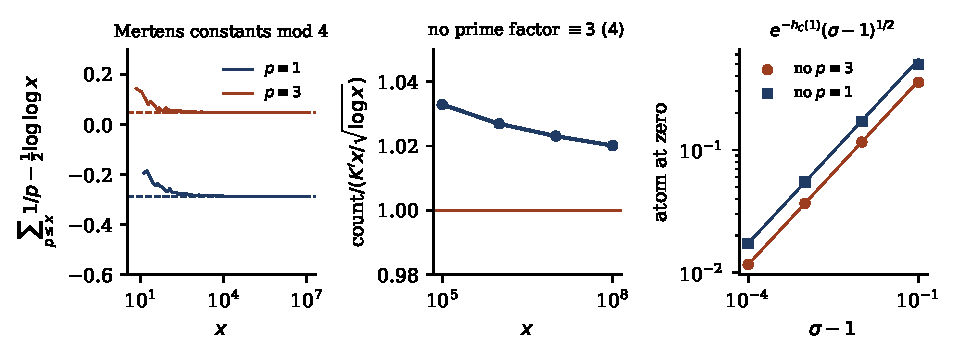
\includegraphics[width=\textwidth]{figs/gl1_landau.pdf}
\caption{Dirichlet's theorem in law for $q=4$. Left: the running sums $\sum_{p\le x,\,p\equiv a}p^{-1}-\frac12\log\log x$ for the two classes, converging to the Mertens constants $M(4,1)=-0.2867$ and $M(4,3)=0.0482$ computed from $L(1,\chi_4)$ (dashed). Middle: the number of integers below $x$ with no prime factor congruent to $3$ modulo $4$, divided by $K'x/\sqrt{\log x}$ with $K'=0.654259$; the excess decays like $1/\log x$. Right: the probability that the zeta distributed integer has no prime factor in a class modulo $4$, against $e^{-h_C(1)}(\sigma-1)^{1/2}$.}\label{fig:gl1landau}
\end{figure}

The atom at zero has a classical counterpart for the uniform integer, due to Landau, which Theorem~\ref{thm:pdrate} identifies with its constant.

\begin{theorem}[Landau's theorem with Wirsing's constant]\label{thm:gl1landau}
The number of $n\le x$ all of whose odd prime factors are congruent to $1$ modulo $4$ is
\[
K'\frac{x}{\sqrt{\log x}}(1+o(1)),\qquad K'=\Bigl(\tfrac12\prod_{p\equiv3\,(4)}(1-p^{-2})\Bigr)^{1/2}=0.654259\ldots
\]
By comparison the number of $n\le x$ that are sums of two squares is $Kx/\sqrt{\log x}$ with the Landau Ramanujan constant $K=(2\prod_{p\equiv3}(1-p^{-2}))^{-1/2}=0.764224\ldots$, and $K'/K=\prod_{p\equiv3\,(4)}(1-p^{-2})=0.856109$, the probability that an integer is not divisible by the square of any prime congruent to $3$ modulo $4$.
\end{theorem}

\begin{proof}
The generating Dirichlet series is $F(s)=(1-2^{-s})^{-1}\prod_{p\equiv1}(1-p^{-s})^{-1}$ and, by the identity above, $F(s)^2=(1-2^{-s})^{-1}\zeta(s)L(s,\chi_4)\prod_{p\equiv3}(1-p^{-2s})$, so $F(s)\sim C(s-1)^{-1/2}$ with $C^2=2L(1,\chi_4)\prod_{p\equiv3}(1-p^{-2})=\frac\pi2\prod_{p\equiv3}(1-p^{-2})$. The coefficients of $F$ are the indicator of the set, a multiplicative function with values in $\{0,1\}$ whose sum over primes $p\le x$ is $\frac12x/\log x$, so Wirsing's theorem \cite{wirsing1961}, in the form used in Theorem~\ref{thm:pdrate}, gives the count $Cx(\log x)^{-1/2}/\Gamma(\frac12)$, and $C/\sqrt\pi=K'$. In the notation of Theorem~\ref{thm:pdrate}, $K'=e^{-h_3(1)}/\Gamma(\frac12)$ with $e^{-h_3(1)}=1.159643$ as computed above, since the integers counted are exactly those with no prime factor in the class of $3$. The sums of two squares have generating series $\bigl(\zeta(s)L(s,\chi_4)(1-2^{-s})^{-1}\prod_{p\equiv3}(1-p^{-2s})^{-1}\bigr)^{1/2}$, which gives $K$ \cite{landau1908}.
\end{proof}

A sieve to $10^8$ gives counts $19915$, $180751$, $1667197$ and $15550333$ at $x=10^5,\dots,10^8$, which are $1.033$, $1.027$, $1.023$ and $1.020$ times $K'x/\sqrt{\log x}$ (Figure~\ref{fig:gl1landau}, left); the excess is the secondary term $c/\log x$ of the Selberg Delange expansion, with $c\approx0.37$.

\section{Reciprocity for \texorpdfstring{$\GL_1$}{GL1}: class field theory as measurability}\label{sec:gl1cft}

The statements of reciprocity in degree one are these.

\begin{theorem}[Kronecker, Weber; Artin; Hecke]\label{thm:gl1cft}
\begin{enumerate}
\item[(i)] Every continuous one dimensional representation of $\Gal(\overline\Q/\Q)$ factors through $\Gal(\Q(\zeta_q)/\Q)$ for some $q$, hence is a Dirichlet character.
\item[(ii)] For a number field $K$ and a modulus $\mathfrak f$, the Artin map $\mathfrak p\mapsto\Frob_{\mathfrak p}$ induces an isomorphism from the ray class group modulo $\mathfrak f$ onto $\Gal(K_{\mathfrak f}/K)$, $K_{\mathfrak f}$ the ray class field, and every abelian extension of $K$ lies in some $K_{\mathfrak f}$. Hence the one dimensional representations of $\Gal(\overline K/K)$ are the characters of ray class groups.
\item[(iii)] A Hecke character of $K$ is a character $\psi$ of the group of fractional ideals prime to $\mathfrak f$ for which there is a continuous character $\psi_\infty$ of $(K\otimes\R)^\times$ with $\psi((\alpha))=\psi_\infty(\alpha)^{-1}$, or $\psi_\infty(\alpha)$ in the convention of this book, for $\alpha\equiv1$ modulo $\mathfrak f$. Its $L$ function $L(s,\psi)=\prod_{\mathfrak p\nmid\mathfrak f}(1-\psi(\mathfrak p)N\mathfrak p^{-s})^{-1}$ has meromorphic continuation and a functional equation, and is entire unless $\psi$ is a power of the norm.
\end{enumerate}
\end{theorem}

The characters of finite order in (iii) are the ray class characters of (ii); the characters of infinite order, Hecke's Gr\"ossencharaktere \cite{hecke1920}, are the automorphic representations of $\GL_1(\A_K)$ that are not Artin representations (the algebraic ones among them are $\ell$ adic characters of $\Gal(\overline K/K)$, which is how $\psi$ appears in Section~\ref{sec:gl1cm}), and they are the subject of Sections~\ref{sec:gl1hecke} and \ref{sec:gl1cm}.

The probabilistic reading is Proposition~\ref{prop:recipcongruence}: a Frobenius random variable $p\mapsto\rho(\Frob_p)$ on the probability space of primes is measurable with respect to the congruence $\sigma$ algebra, the one generated by the events $\{p\equiv a\ (q)\}$, if and only if $\rho$ is abelian. Theorem~\ref{thm:gl1cft}(i) is the statement that for one dimensional $\rho$ this is always so. The Dirichlet process of Theorem~\ref{thm:gl1dirichlet} is the normalised Gamma process of Theorem~\ref{thm:recipgammaproc} seen through that $\sigma$ algebra, and its base measure is uniform because the Frobenius elements of an abelian extension of $\Q$ are equidistributed in the Galois group, which is Dirichlet's theorem again.

\section{Hecke characters of \texorpdfstring{$\Q(i)$}{Q(i)} and the angles of Gaussian primes}\label{sec:gl1hecke}

Let $K=\Q(i)$, with ring of integers $\Z[i]$, units $\{\pm1,\pm i\}$, and class number one. A prime $p\equiv1$ modulo $4$ splits as $p=\pi\bar\pi$ with $\pi=a+bi$, $p=a^2+b^2$; a prime $p\equiv3$ stays prime, with residue degree two; and $2=-i(1+i)^2$ ramifies. Among the four associates of $\pi$ exactly one is \emph{primary}, $\pi\equiv1$ modulo $(2+2i)$, which for $a+bi$ means $a$ odd, $b$ even and $a+b\equiv1$ modulo $4$; the primary generator is the one used by Gauss for biquadratic reciprocity. Both $\pi$ and $\bar\pi$ are primary. Write $\theta_p=|\arg\pi|\in[0,\pi]$, which is the same for both, and note that the argument of any generator is $\pm\theta_p$ plus a multiple of $\pi/2$, so $4\theta_p$ modulo $2\pi$ is well defined up to sign.

For $k\in\Z$ the function $\lambda_k((\alpha))=(\alpha/|\alpha|)^{4k}$ is well defined on all nonzero ideals, since the units are fourth roots of unity, and it is a Hecke character of $K$ with trivial conductor and infinity type $z\mapsto(z/|z|)^{4k}$. Its $L$ function $L(s,\lambda_k)$ is entire for $k\ne0$ and does not vanish on $\operatorname{Re}s=1$ (Hecke).

\begin{theorem}[Hecke \cite{hecke1920}]\label{thm:gl1hecke}
The angles $4\theta_p$, $p\equiv1$ modulo $4$, are equidistributed modulo $2\pi$: for every continuous $f$ on the circle, $\frac1{\pi_1(x)}\sum_{p\le x,\,p\equiv1}f(4\theta_p)\to\frac1{2\pi}\int_0^{2\pi}f$. More precisely the arguments of the primary Gaussian primes, both $\pi$ and $\bar\pi$ for each $p$, are equidistributed on the circle, so that $\theta_p$ is equidistributed on $[0,\pi]$.
\end{theorem}

\begin{proof}
By Weyl's criterion it suffices that $\sum_{p\le x,p\equiv1}e^{4ik\theta_p}=o(x/\log x)$ for $k\ne0$. The sum is $\sum_{N\mathfrak p\le x}\lambda_k(\mathfrak p)$ over the degree one primes of $K$, up to the $O(\sqrt x)$ primes of degree two, and the prime ideal theorem for $L(s,\lambda_k)$, that is the nonvanishing on $\operatorname{Re}s=1$ with the Wiener Ikehara theorem applied to $-L'/L$, gives $\sum_{N\mathfrak p\le x}\lambda_k(\mathfrak p)=o(x/\log x)$. For the primary arguments the same argument applies to the Hecke characters $\lambda'_m((\alpha))=(\alpha/|\alpha|)^m$, $\alpha\equiv1$ modulo $(2+2i)$, which are well defined for every $m$ because $1$ is the only unit congruent to $1$ modulo $(2+2i)$, and whose $L$ functions are entire and nonvanishing on $\operatorname{Re}s=1$ for $m\ne0$; the sum over the degree one primes of $K$ runs over both $\pi$ and $\bar\pi$, and the symmetric law of the pair $\{\theta_p,-\theta_p\}$ is uniform on the circle if and only if $\theta_p$ is uniform on $[0,\pi]$.
\end{proof}

The angles of the $332180$ Gaussian primes below $10^7$ have discrepancy $D=0.00145$ from the uniform law, $\sqrt nD=0.84$, and Weyl sums $|\frac1n\sum e^{4ik\theta_p}|$ between $6\cdot10^{-4}$ and $1.1\cdot10^{-3}$ for $k\le5$, against $n^{-1/2}=1.7\cdot10^{-3}$ for independent uniform angles (Figure~\ref{fig:gl1hecke}, left). Under GRH for the $L(s,\lambda_k)$ the number of Gaussian primes below $x$ in an arc is its expected value up to $O(\sqrt x\log^2x)$, and the Weyl sums are of the size of a random walk, as here.

\begin{figure}[t]
\centering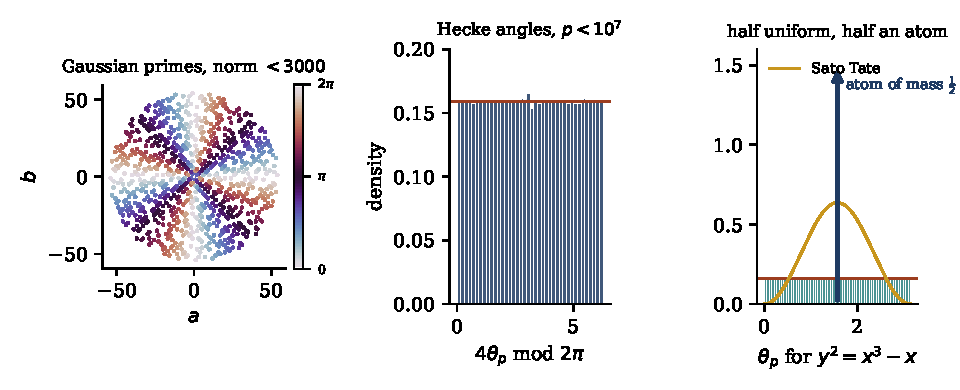
\includegraphics[width=\textwidth]{figs/gl1_hecke.pdf}
\caption{Left: the Gaussian primes of norm below $3000$ with their four associates, coloured by the Hecke angle $4\theta_p$. Middle: the angles $4\theta_p$ of the Gaussian primes below $10^7$ against the uniform law. Right: the Frobenius angles $\theta_p$ of $y^2=x^3-x$, uniform on $[0,\pi]$ for the split primes and equal to $\pi/2$ for the inert primes, against the Sato Tate density of a curve without complex multiplication.}\label{fig:gl1hecke}
\end{figure}

Hecke's theorem is Chebotarev's theorem for an infinite extension: the characters $\lambda_k$ do not factor through any finite Galois group, and the ``Galois group'' in which the Frobenius elements equidistribute is the circle, the connected component of the Sato Tate group of Section~\ref{sec:gl1cm}. The Gamma process of Theorem~\ref{thm:recipgammaproc} applies to the random integer coloured by $4\theta_p$ with $Y$ the circle and $\mu$ uniform, so that for a continuous $Q\ge0$ on the circle the Frobenius functional $\Xi_\sigma(Q)=(\sigma-1)\sum_{p\equiv1}e_p\log p\,Q(4\theta_p)$ converges to a GGC with Thorin measure $\frac12$ times the image of the uniform law under $1/Q$, the factor $\frac12$ being the density of the split primes, and the labelled factorisation converges to a Dirichlet process whose base measure is $\frac12$ times the uniform probability on the circle. The Mertens constants are given by Theorem~\ref{thm:pdmertensL} with the $L(1,\lambda_k)$ in place of the $L(1,\chi)$: for a trigonometric polynomial $Q(y)=\sum_{|k|\le m}c_ke^{iky}$, $\sum_{p\le x,\,p\equiv1}Q(4\theta_p)p^{-1}=\frac12c_0\log\log x+M(Q)+o(1)$ with $M(Q)=\frac12c_0M(4,1)+\frac12\sum_{0<|k|\le m}c_kS(\lambda_k)$, $S(\lambda_k)=\log L(1,\lambda_k)-\sum_{j\ge2}\sum_{\mathfrak p}\lambda_k(\mathfrak p)^j(jN\mathfrak p^j)^{-1}$; for the indicator of an arc the Fourier series of $M$ converges only conditionally and is better handled by smoothing.

\section{Complex multiplication}\label{sec:gl1cm}

Let $E$ be the curve $y^2=x^3-x$, of conductor $32$, with the automorphism $(x,y)\mapsto(-x,iy)$ giving complex multiplication by $\Z[i]$. Let $\psi$ be the Hecke character of $K=\Q(i)$ of conductor $\mathfrak f=(2+2i)$ with $\psi((\alpha))=\alpha$ for $\alpha\equiv1$ modulo $\mathfrak f$; it is well defined because $1$ is the only unit congruent to $1$ modulo $\mathfrak f$, and its infinity type is the identity. At the inert prime $(p)$, $p\equiv3$ modulo $4$, the primary generator is $-p$, since $4\in\mathfrak f$, so $\psi((p))=-p$.

\begin{theorem}[Deuring \cite{deuring1953}]\label{thm:gl1deuring}
$L(E,s)=L(s,\psi)$. Explicitly, for $p\equiv1$ modulo $4$ with primary $\pi=a+bi$, $a_p(E)=\pi+\bar\pi=2a$; for $p\equiv3$, $a_p(E)=0$; and the Euler factor at $p\equiv3$ is $(1+p^{1-2s})^{-1}$ on both sides.
\end{theorem}

The identity $a_p=2a$ with the primary normalisation was checked for all $332180$ primes $p\equiv1$ modulo $4$ below $10^7$ against the point counts of PARI; it holds without exception, and the other associates $-\pi$, $i\pi$, $-i\pi$ fail at every prime. The general theorem is that for $E/\Q$ with complex multiplication by an imaginary quadratic $K$, $L(E,s)=L(s,\psi)$ for a Hecke character $\psi$ of $K$ of infinity type the identity and conductor $\mathfrak f$ with $N_E=|d_K|N\mathfrak f$; here $32=4\cdot8$.

Deuring's theorem is reciprocity for $\GL_2$ reduced to $\GL_1$: the two dimensional representation $\rho_E$ of $\Gal(\overline\Q/\Q)$ is induced from the one dimensional representation $\psi$ of $\Gal(\overline\Q/K)$, which is abelian, so that $\rho_E$ is \emph{dihedral}, and its automorphic partner is the automorphic induction of $\psi$, the theta series $\sum_{\mathfrak a}\psi(\mathfrak a)q^{N\mathfrak a}$, a weight two form of level $32$ (Hecke). In the language of Chapter~\ref{ch:recip}, reciprocity for $E$ is the almost sure equality of $p\mapsto a_p(E)$ and $p\mapsto\pi+\bar\pi$, which Theorem~\ref{thm:gl1deuring} proves prime by prime.

\begin{proposition}[the angle law of a CM curve]\label{prop:gl1angle}
Write $a_p(E)=2\sqrt p\cos\theta_p$ with $\theta_p\in[0,\pi]$. Then $\theta_p$ is the angle of Section~\ref{sec:gl1hecke} for split $p$ and $\theta_p=\pi/2$ for inert $p$, and the law of $\theta_p$ is $\frac12\,\mathrm{Unif}[0,\pi]+\frac12\delta_{\pi/2}$. The moments are $\E\cos^2\theta_p=\frac14$ and $\E\cos^4\theta_p=\frac3{16}$, against $\frac14$ and $\frac18$ for the Sato Tate law; below $10^7$ the sample values are $0.24988$ and $0.18738$.
\end{proposition}

\begin{proof}
For split $p$, $\cos\theta_p=a/\sqrt p=\cos\arg\pi$ by Theorem~\ref{thm:gl1deuring}, and $|\arg\pi|$ is uniform on $[0,\pi]$ by the second part of Theorem~\ref{thm:gl1hecke}. The two classes have density $\frac12$ each by Dirichlet.
\end{proof}

The law in Proposition~\ref{prop:gl1angle} is the law of the trace of a Haar distributed element of the normaliser $N(\mathrm{U}(1))$ of the maximal torus $\mathrm{U}(1)$ in $\SU(2)$: the identity component contributes the uniform angle, the other component consists of matrices of trace zero. This is the Sato Tate group of a CM curve, and Chapter~\ref{ch:12} identifies it from the moments.

Now take the Rankin Selberg subordinator $X_\sigma$ of Section~\ref{sec:recipgalois}, with Laplace transform $D^S(\sigma+\lambda)/D^S(\sigma)$, $D^S(s)=L^S(s,\rho\otimes\check\rho)$, built over $\Q$, and the same subordinator $X^K_\sigma$ built over $K$ from the restriction of $\rho$ to $\Gal(\overline\Q/K)$, with $D^S_K(s)=L^S_K(s,\rho|_K\otimes\check\rho|_K)$ an Euler product over the primes of $K$.

\begin{theorem}[complex multiplication doubles the Gamma shape; this book]\label{thm:gl1cmshape}
Let $E/\Q$ be an elliptic curve, $\rho$ its normalised $\ell$ adic representation, $K$ an imaginary quadratic field and $\chi_K$ its character.
\begin{enumerate}
\item[(i)] $D^S_K(s)=D^S(s)\,L^S(s,\rho\otimes\check\rho\otimes\chi_K)$, the partial products being over the primes not dividing $N_E d_K$.
\item[(ii)] If $E$ has complex multiplication by $K$ then $D^S_K(s)=D^S(s)^2$ exactly, so that $X^K_\sigma$ has the law of the sum of two independent copies of $X_\sigma$ for every $\sigma>1$, and $(\sigma-1)X^K_\sigma$ converges to the Gamma law of shape $2$.
\item[(iii)] If $E$ has no complex multiplication by $K$ then $(\sigma-1)X^K_\sigma$ converges to the standard exponential law, the Gamma shape being $1$.
\end{enumerate}
\end{theorem}

\begin{proof}
(i) Restriction followed by induction multiplies by the regular representation of $\Gal(K/\Q)$: $\operatorname{Ind}_K^\Q\operatorname{Res}_K(\rho\otimes\check\rho)=(\rho\otimes\check\rho)\otimes(\mathsf 1\oplus\chi_K)$, and the $L$ function of an induced representation is the $L$ function over the smaller field of the representation induced from. At the level of Euler factors this is the statement that a prime $p$ of $\Q$ split in $K$ contributes two identical factors over $K$, while an inert $p$ contributes one factor at $p^2$, which equals the product of the factors of $\rho\otimes\check\rho$ and $\rho\otimes\check\rho\otimes\chi_K$ at $p$.

(ii) If $E$ has complex multiplication by $K$ then $a_p=0$ for every inert $p$, so $\tr\rho(\Frob_p)\chi_K(p)=\tr\rho(\Frob_p)$ for all $p\nmid N_Ed_K$, and $\rho\otimes\chi_K\cong\rho$ by Brauer and Nesbitt, both being semisimple. Hence $\rho\otimes\check\rho\otimes\chi_K\cong\rho\otimes\check\rho$, the two factors in (i) coincide, and $D_K^S=(D^S)^2$. A squared Laplace transform is the transform of a sum of two independent copies. By Theorem~\ref{thm:recipgamma} and its proof, which use only the order of the pole of $D^S$ at $s=1$, the Gamma shape is twice the shape over $\Q$, which is $1$ because $\rho$ is irreducible.

(iii) Over $K$ the Gamma shape is the order of the pole of $D^S_K$ at $1$, which by (i) is $1+m$, $m$ the order of the pole of $L(s,\rho\otimes\check\rho\otimes\chi_K)$. By modularity and the theory of Rankin and Selberg, $L(s,\rho\otimes\check\rho\otimes\chi_K)=L(s,f\times(f\otimes\chi_K))$ for the newform $f$ of $E$, and this has a pole at $s=1$ if and only if $f\otimes\chi_K=f$, that is $\rho\otimes\chi_K\cong\rho$, which forces $a_p=0$ for all inert $p$ of $K$, a set of density $\frac12$. For a curve without complex multiplication the primes with $a_p=0$ have density zero (Serre), and for a curve with complex multiplication by a field $K'\ne K$ they are, up to finitely many, the primes inert in $K'$, which exclude the primes split in $K'$ and inert in $K$, a set of density $\frac14$. So $f\otimes\chi_K=f$ forces complex multiplication by $K$, hence $m=0$ and the shape is $1$.
\end{proof}

For the curve $y^2=x^3-x$ the Laplace transforms were computed exactly from $D^S(s)=\zeta^{(2)}(s)L(s+1,\Sym^2E)$, the symmetric square from PARI, whose Euler factor at $2$ is trivial; this identity is the decomposition $\rho\otimes\check\rho=\mathsf 1\oplus\chi_4\oplus\operatorname{Ind}\tilde\psi^2$ together with $\Sym^2\rho=\operatorname{Ind}\tilde\psi^2\oplus\chi_4$. At $\sigma=1.001$ the transform of $(\sigma-1)X_\sigma$ at $\lambda=\frac12,1,2,4,8$ is $0.6672$, $0.5009$, $0.3345$, $0.2014$, $0.1127$ against $(1+\lambda)^{-1}=0.6667$, $0.5$, $0.3333$, $0.2$, $0.1111$, and over $K$ the squares $0.4452$, $0.2509$, $0.1119$, $0.0406$, $0.0127$ against $(1+\lambda)^{-2}$. The approach is at the rate $\sigma-1$ of the Euler Kronecker drift (Theorem~\ref{thm:recipdrift}): the deviations at $\lambda=1$ are $0.0810$, $0.0086$ and $0.0009$ at $\sigma-1=10^{-1},10^{-2},10^{-3}$ (Figure~\ref{fig:gl1cm}, left).

\begin{figure}[t]
\centering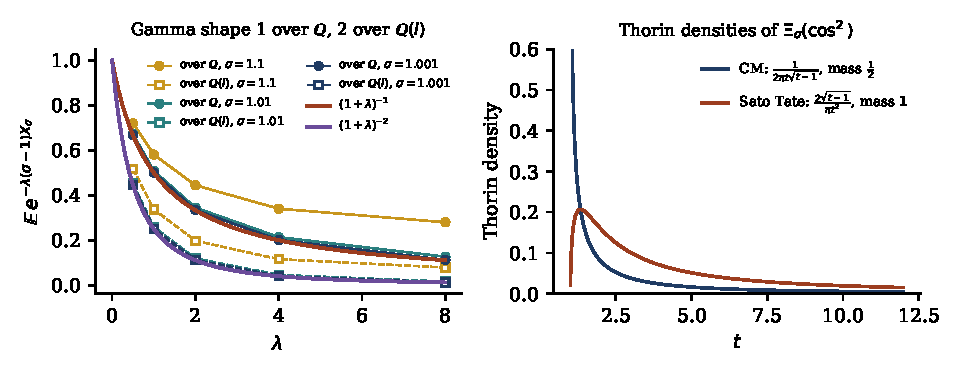
\includegraphics[width=\textwidth]{figs/gl1_cm.pdf}
\caption{Complex multiplication doubles the Gamma shape. Left: the Laplace transforms of $(\sigma-1)X_\sigma$ for $y^2=x^3-x$ over $\Q$ and over $\Q(i)$ at three values of $\sigma$, against the exponential and the Gamma$(2)$ limits of Theorem~\ref{thm:gl1cmshape}. Right: the Thorin densities of the limiting Frobenius functional $\Xi_\sigma(\cos^2)$ for a CM curve, the arcsine density of mass $\frac12$, and for a curve without complex multiplication, the image of the Sato Tate law, of mass $1$.}\label{fig:gl1cm}
\end{figure}

Theorem~\ref{thm:gl1cmshape} says what the Gamma shape of Chapter~\ref{ch:recip} measures when the base field changes: it counts the irreducible constituents with multiplicity, and restriction to $K$ splits $\rho$ exactly when $\rho$ is induced from $K$. For a CM curve the restriction is $\tilde\psi\oplus\tilde\psi^c$, two distinct characters, and the shape is $1^2+1^2=2$; a curve without complex multiplication by $K$ stays irreducible over $K$ and keeps shape $1$. The test is unconditional because both pole orders are theorems.

Finally the Frobenius functionals. Colour the prime factors of $N_\sigma$ by $y_p=4\theta_p$ on the circle for split $p$ and by a point $\{\mathrm{in}\}$ for inert $p$, so $Y=S^1\sqcup\{\mathrm{in}\}$ with $\mu=\frac12\mathrm{Unif}+\frac12\delta_{\mathrm{in}}$. Theorem~\ref{thm:recipggcfun} gives, for continuous $Q\ge0$ on $Y$, the GGC limit of $\Xi_\sigma(Q)$ with Thorin measure the image of $\mu$ under $1/Q$ on $\{Q>0\}$. Two cases are instructive. For $Q=\mathsf 1_{\mathrm{in}}$ the limit is the Gamma law of shape $\frac12$, with Thorin measure $\frac12\delta_1$, and the atom at zero $e^{-h_3(1)}(\sigma-1)^{1/2}$ is the Landau phenomenon of Theorem~\ref{thm:gl1landau}. For $Q=\cos^2\theta_p=a^2/p$, a quarter of the squared normalised trace, the limit has Thorin measure $\frac12$ times the image of the uniform law on $[0,\pi]$ under $\theta\mapsto1/\cos^2\theta$, that is the measure $\frac{dt}{2\pi t\sqrt{t-1}}$ on $(1,\infty)$, of total mass $\frac12$ (Figure~\ref{fig:gl1cm}, right): the Frobenius functional $\Xi_\sigma(\cos^2)$ of a CM curve is asymptotically a GGC with an explicit arcsine Thorin density. For a curve without complex multiplication the same functional has the Thorin density $\frac{2}{\pi t^2}\sqrt{t-1}$ of total mass one on $(1,\infty)$, the image of the Sato Tate law.

\section{The Thorin measure of a degree one \texorpdfstring{$L$}{L} function}\label{sec:gl1thorin}

Let $\chi$ be a primitive real character modulo $q$ and $\kappa\in\{0,1\}$ its parity, so that the completed function $\Lambda(s,\chi)=(q/\pi)^{s/2}\Gamma(\frac{s+\kappa}2)L(s,\chi)$ satisfies $\Lambda(s,\chi)=\Lambda(1-s,\chi)$ with root number $+1$. Put $\Xi_\chi(w)=\Lambda(\frac12+w,\chi)$, an even entire function of order one, and write its zeros as $\pm i\gamma_k$, with multiplicity, choosing one $\gamma_k$ from each pair; only $\gamma_k^2$ enters below.

\begin{theorem}[Thorin form in degree one]\label{thm:gl1thorin}
Suppose $L(\frac12,\chi)\ne0$. Then $\Xi_\chi(\sqrt\lambda)/\Xi_\chi(0)=\prod_k(1+\lambda/\gamma_k^2)$ for $\lambda\ge0$, the product converging absolutely, and GRH for $\chi$ holds if and only if $\Xi_\chi(0)/\Xi_\chi(\sqrt\lambda)$ is the Laplace transform of a GGC, in which case the Thorin measure is $\sum_k\delta_{\gamma_k^2}$ and the GGC is $\sum_kE_k/\gamma_k^2$ with $E_k$ independent standard exponentials. For every basepoint $\frac12+a$ with $a\ge\frac12$ the shifted representation of Theorem~\ref{thm:10dshift} holds unconditionally, with the Thorin density $V_a$ positive.
\end{theorem}

\begin{proof}
This is Theorem~\ref{thm:10bmain} for $n=1$, which Section~\ref{sec:10bcompletion} admits; the proof reads: $\Xi_\chi$ is even and entire of order one, so Hadamard's product has the form $e^{bw}\prod(1+w^2/\gamma_k^2)$ with $b=0$ by evenness, and $\Xi_\chi(0)\ne0$ by hypothesis. The nonvanishing hypothesis holds for $\chi_4$, where $L(\frac12,\chi_4)=0.6677$, and is Chowla's conjecture for real $\chi$ in general; a zero of order $2m$ at $w=0$ is removed by dividing by $w^{2m}$ and changes nothing else. The last assertion is Theorem~\ref{thm:10dshift}(iii).
\end{proof}

For $\chi_4$ the first zeros are at $\gamma=6.020949$, $10.243770$, $12.988098$, $16.342607$, $18.291993$, and there are $3130$ below height $3000$, where the counting function $\frac T{2\pi}\log\frac{4T}{2\pi e}$ predicts $3129.7$. With these zeros and the tail $\int_T^\infty\log(1+\lambda/t^2)\,dN(t)$ from the smooth counting function, the product $\prod_k(1+\lambda/\gamma_k^2)$ agrees with $\Xi_{\chi_4}(\sqrt\lambda)/\Xi_{\chi_4}(0)$ to relative error $2\cdot10^{-8}$ at $\lambda=1$, $3\cdot10^{-7}$ at $\lambda=16$, $2\cdot10^{-6}$ at $\lambda=100$ and $9\cdot10^{-6}$ at $\lambda=400$, where the ratio is $2.8\cdot10^7$; the residual error is the tail approximation, which grows with $\lambda$ (Figure~\ref{fig:gl1zeros}, left). The right panel of the figure shows the Thorin density of Theorem~\ref{thm:10dshift} at three basepoints $\frac12+a$: by Theorem~\ref{thm:lapcauchy} it is the measure $\sum_k\delta_{\gamma_k}$ on the $\sqrt z$ axis smoothed by Cauchy noise of scale $a$, and as $a\downarrow0$ the peaks sharpen into the atoms $\delta_{\gamma_k^2}$ of Theorem~\ref{thm:gl1thorin}.

\begin{figure}[t]
\centering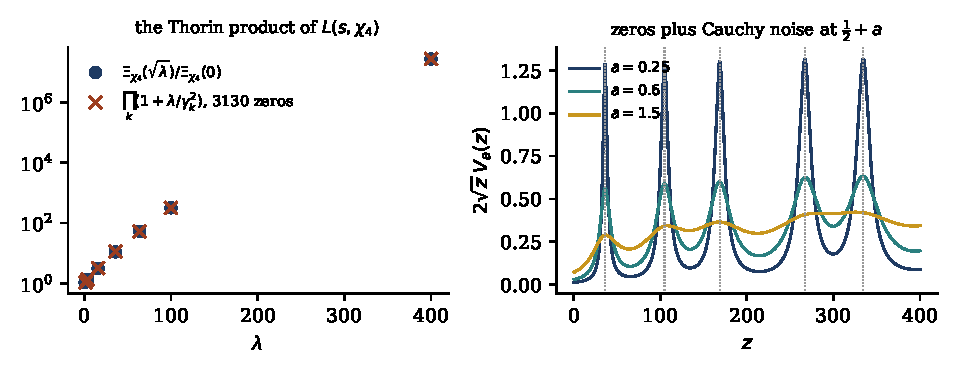
\includegraphics[width=\textwidth]{figs/gl1_zeros.pdf}
\caption{The Thorin measure of $L(s,\chi_4)$. Left: $\Xi_{\chi_4}(\sqrt\lambda)/\Xi_{\chi_4}(0)$ against the product over the $3130$ zeros below height $3000$ with the tail correction; the two agree to between $2\cdot10^{-8}$ and $9\cdot10^{-6}$. Right: the shifted Thorin density $V_a(z)$ of Theorem~\ref{thm:10dshift}, drawn as $2\sqrt zV_a(z)=\frac1\pi\sum_k\bigl[\frac{a}{a^2+(\sqrt z-\gamma_k)^2}+\frac{a}{a^2+(\sqrt z+\gamma_k)^2}\bigr]$, for $a=0.25$, $0.6$ and $1.5$; the vertical lines mark $\gamma_k^2$ for the first five zeros.}\label{fig:gl1zeros}
\end{figure}

The Galois face is different in degree one from degree two, and the difference is worth recording. The sine squared lemma (Lemma~\ref{lem:10dsin2}) represents $f(\alpha)/f(\alpha+\sqrt\lambda)$ through a GGC when $\log f(\alpha+s)$ is the Laplace transform of a positive measure, as it is for $\zeta$, for $\zeta_K$, and for every Rankin Selberg $L$ function. For $L(s,\chi)$ with $\chi$ real the logarithmic coefficients $\chi(p)^k\log p/k$ change sign, and the formula of the lemma produces a signed density: for small $z$ it is $-\frac{\sqrt z}{4\pi}(\log L)'''(\alpha)=\frac{\sqrt z}{4\pi}\sum_n\Lambda_\chi(n)(\log n)^2n^{-\alpha}$, which for $\chi_4$ equals $-0.257$, $-0.156$, $-0.090$ at $\alpha=1.1,1.5,2$, whereas for $\zeta_{\Q(i)}=\zeta L(\cdot,\chi_4)$ the same quantity is $2000$, $15.8$, $1.86$. So on the Galois face a real character is not by itself a GGC object; its Dedekind zeta function is, and so is its completed $L$ function at every basepoint $\alpha\ge1$ by Theorem~\ref{thm:gl1thorin}, the gamma factor supplying the positivity that the Euler product lacks. This is the degree one instance of the remark in Chapter~\ref{ch:lap} that the two faces carry the same measure but not the same positivity.

\section{What this adds to the programme}

The chapter proves, in degree one, the three things that the rest of the book conjectures or assumes in degree two: equidistribution with the right base measure (Dirichlet, Hecke), reciprocity (Kronecker Weber, Artin, Deuring), and the Thorin structure at every basepoint to the right of the zeros. Two of its theorems are new in substance. Theorem~\ref{thm:gl1landau}, whose constant is a standard application of Landau and Wirsing, identifies the Wirsing constant of the atom at zero of Chapter~\ref{ch:pd} with Landau's constant, corrected by the probability $\prod_{p\equiv3}(1-p^{-2})$ of squarefreeness in the class, and locates Landau's theorem inside the Dirichlet process. Theorem~\ref{thm:gl1cmshape} shows that the Gamma shape of Theorem~\ref{thm:recipgamma}, which detects irreducibility over $\Q$, detects complex multiplication when the base field is changed, with an exact identity $D_K^S=(D^S)^2$ rather than an asymptotic one. It also shows what the Gamma shape cannot do: over $\Q$ a CM curve and a non CM curve both have shape $1$, and the difference between them is visible only in the Thorin measure of the Frobenius functionals (an arcsine density of mass $\frac12$ against a Sato Tate density of mass $1$) or after base change.

\section{Notes}

The theorem of Kronecker and Weber, Artin's reciprocity law and Hecke's Gr\"ossencharaktere are in any account of class field theory; Neukirch \cite{neukirch1999} is the reference used here, and Tate's thesis \cite{tate1950} is the adelic form of Theorem~\ref{thm:gl1cft}(iii). Hecke's equidistribution theorem is \cite{hecke1920}; its discrepancy under GRH is treated by Kubilius \cite{kubilius1955}. Mertens' theorem for progressions is due to Williams \cite{williams1974}. Landau's theorem on sums of two squares is \cite{landau1908}; the constant is often attributed jointly to Ramanujan, and Wirsing's theorem \cite{wirsing1961} is the general form. Deuring's theorem is \cite{deuring1953}; Silverman's second volume \cite{silverman1994} gives the proof and the computation of the Hecke character of $y^2=x^3-x$, and Ireland and Rosen \cite{irelandrosen1990} the elementary count $a_p=2a$ with the primary normalisation. The Rankin Selberg criterion for $f\otimes\chi=f$ used in Theorem~\ref{thm:gl1cmshape} is in \cite{iwanieckowalski2004}. Theorem~\ref{thm:gl1dirichlet}(iii) is Williams' theorem, and (i) and (ii) are its Dirichlet process reading; Theorem~\ref{thm:gl1landau} is classical apart from the identification with $h_3(1)$; Theorems~\ref{thm:gl1cmshape} and \ref{thm:gl1thorin} are new as formulated. Their ingredients are the theorems cited and Chapters~\ref{ch:10b}, \ref{ch:recip} and \ref{ch:pd}.

\section{Exercises}

\begin{enumerate}
\item Show that among the four associates $\pm\pi,\pm i\pi$ of a Gaussian prime exactly two, $\pi$ and $-\pi$, have odd real part, and that $a_p=2\operatorname{Re}\pi$ holds for the primary one only. Determine the proportion of primes at which the normalisation $a\equiv1$ modulo $4$ alone gives the right sign.
\item Compute $M(8,a)$ for the four classes modulo $8$ from $L(1,\chi)$ for the three nonprincipal characters, and check against the primes below $10^7$.
\item Show that the number of $n\le x$ all of whose prime factors are congruent to $1$ modulo $q$ is asymptotic to $c_qx(\log x)^{1/\varphi(q)-1}$, and express $c_q$ through the $L(1,\chi)$.
\item For $E$ with complex multiplication by $K$, show that the Sato Tate group is $N(\mathrm{U}(1))$ and that the moments of $\cos\theta_p$ are $\E\cos^{2m}\theta_p=\frac12\binom{2m}m4^{-m}$. Verify the values $\frac14$ and $\frac3{16}$.
\item Show that for $Q=\cos^2(y/4)$ on the circle the image of the uniform law under $1/Q$ has density $1/(\pi t\sqrt{t-1})$ on $(1,\infty)$, and that the corresponding GGC has Laplace transform $\exp(-\frac12\int_1^\infty\log(1+\lambda/t)\frac{dt}{\pi t\sqrt{t-1}})$. Compute this integral in closed form.
\item Prove Theorem~\ref{thm:gl1cmshape}(i) at the level of Euler factors for a split and for an inert prime.
\item Let $\chi$ be a real character with $L(\frac12,\chi)=0$ of order $2m$. Show that $\Xi_\chi(\sqrt\lambda)/(\lambda^m\Xi_\chi^{(2m)}(0)/(2m)!)$ is again $\prod(1+\lambda/\gamma_k^2)$ over the remaining zeros.
\end{enumerate}

\section{Open problems}

\begin{problem}[the discrepancy of Hecke angles]\label{op:gl1disc}
For the Gaussian primes below $x$ the discrepancy of $4\theta_p$ satisfies $\sqrt{\pi_1(x)}D=1.07$ at $x=10^6$ and $0.84$ at $x=10^7$. Determine whether $\sqrt{\pi_1(x)}D$ has a limit law as $x\to\infty$ (the Kolmogorov law would be the Brownian bridge prediction, as in Open Problem~\ref{op:disc} for Sato Tate), or whether the arithmetic of the $L(s,\lambda_k)$ forces a different law; the same question for the imaginary quadratic fields of class number one.
\end{problem}

\begin{problem}[Euler Kronecker constants of Hecke characters]\label{op:gl1rate}
The rate of convergence of the Dirichlet process of Section~\ref{sec:gl1hecke} is governed, for the means, by the constants $L'/L(1,\lambda_k)$ in the same way that Theorem~\ref{thm:recipdrift} is governed by Euler Kronecker constants. Compute these constants for $\Q(i)$ and $k\le20$, determine the sign pattern of the deficits of the arcs, and find the analogue of Theorem~\ref{thm:pdrate} for the circle, where no arc is a finite union of classes.
\end{problem}

\begin{problem}[an effective Gamma shape test]\label{op:gl1cm}
Theorem~\ref{thm:gl1cmshape} distinguishes complex multiplication by $K$ through a limit as $\sigma\downarrow1$. By Faltings' theorem finitely many $a_p$ determine $\rho$ up to isomorphism, so finitely many primes decide whether $\rho\otimes\chi_K\cong\rho$. Find an explicit bound, in terms of $N_E$ and $d_K$, on the primes needed so that the empirical Laplace transform of $(\sigma-1)X^K_\sigma$ at a suitable $\sigma$ separates shape $1$ from shape $2$ with a proof, and compare with the bound from the effective Chebotarev theorem.
\end{problem}

\begin{compproblem}[class number one fields]\label{cp:gl1}
Objective: for each of the nine imaginary quadratic fields of class number one, compute the Hecke angles of the split primes below $10^9$, their discrepancy, and the Mertens constants of the arcs of length $\pi/2$, with the predicted constants from $L(1,\lambda_k)$. For the CM curves of conductor $27$, $32$, $36$, $49$, $121$ and $256$ verify Theorem~\ref{thm:gl1cmshape}(ii) from the exact Laplace transforms at $\sigma=1.0001$. Starting point: \texttt{g1.py}, \texttt{g3.py} and \texttt{g4.py}.
\end{compproblem}

\chapter[Maass Forms and Brownian Motion]{Maass Forms, the Selberg Trace Formula\\ and Brownian Motion on the Modular Surface}\label{ch:maass}

The holomorphic modular forms of Chapter~\ref{ch:02} are half of the automorphic spectrum of $\SL_2(\Z)$. The other half consists of the Maass forms, the eigenfunctions of the hyperbolic Laplacian on the modular surface $X=\SL_2(\Z)\backslash\mathbb H$, and the book has so far mentioned them only in passing. They matter to its programme for two reasons. The first is that the Galois representations on the Maass side are the even ones, which the gamma factor of the Galois heat trace of Chapter~\ref{ch:recip} tells apart from the odd ones (Section~\ref{sec:msquarter}): an even two dimensional Artin representation corresponds, when it corresponds to anything, to a Maass form of eigenvalue exactly $\frac14$, and the even icosahedral case is the one two dimensional case of reciprocity that is open. The second is that the Selberg trace formula, the fundamental identity of the Maass side, is a heat trace identity of precisely the shape of the Galois heat trace of Chapter~\ref{ch:recip}, with closed geodesics in the place of primes, and its probabilistic content is Brownian motion on $X$: the sum of $e^{-t\lambda_j}$ over the Laplace spectrum is the return density of Brownian motion integrated over the surface, decomposed by the homotopy class of the loop the path has made.

This chapter sets out the spectral theory of $X$ in the language of the book. The modular surface is a probability space with the normalised hyperbolic area, Brownian motion on it is ergodic with that law, and the heat kernel decomposes over Maass forms and Eisenstein series. The Selberg trace formula is stated for compact quotients, where it is clean, and read through Brownian loops. Two theorems transcribe the book's dictionary to this setting: Selberg's eigenvalue conjecture is the complete monotonicity of the heat trace, exactly as GRH is the complete monotonicity of the Galois heat trace, and is a theorem for $\SL_2(\Z)$ and within $(\frac7{64})^2$ of a theorem in general; and the closed geodesics, ordered by length, form a Beurling system of primes to which the Poisson Dirichlet theory of Chapter~\ref{ch:pd} and the sine squared lemma of Chapter~\ref{ch:10d} apply without change, so that the geodesic Euler product $Z(s+1)/Z(s)$ is represented unconditionally through a GGC at every basepoint to the right of $1$. The chapter also records an obstruction: Weyl's law places the Laplace spectrum just outside the Thorin class at the centre, because $\sum_j r_j^{-2}$ diverges, whereas $\sum_\gamma\gamma^{-2}$ over the zeros of an $L$ function converges. The last section states and checks the Eichler Selberg trace formula, the holomorphic analogue that Chapter~\ref{ch:07} uses, and reads it as the moment identity behind Serre's vertical Sato Tate law.

\section{The modular surface as a probability space}\label{sec:mssurface}

Let $\mathbb H=\{z=x+iy:\ y>0\}$ with the hyperbolic metric $ds^2=(dx^2+dy^2)/y^2$, area element $d\mu=dx\,dy/y^2$, and Laplacian
\[
\Delta=-y^2\Bigl(\frac{\partial^2}{\partial x^2}+\frac{\partial^2}{\partial y^2}\Bigr),
\]
a nonnegative operator in the sign convention of this chapter. The group $\SL_2(\R)$ acts by isometries, and $\Gamma=\SL_2(\Z)$ acts with the fundamental domain $F=\{|x|\le\frac12,\ |z|\ge1\}$ of area $\pi/3$. The modular surface $X=\Gamma\backslash\mathbb H$ carries the probability measure $\frac3\pi d\mu$; this is the probability space of the chapter. Under it the height $y$ has a heavy tail, $\Prob(y>Y)=3/(\pi Y)$ for $Y\ge1$, so that $y$ has no mean: the cusp carries a vanishing fraction of the area at great height, but not a summable one.

A \emph{Maass form}\index{Maass form} is a $\Gamma$ invariant eigenfunction of $\Delta$ of moderate growth; a Maass cusp form has vanishing constant term in its Fourier expansion, hence is square integrable and decays exponentially in the cusp. The spectral theorem for $L^2(X)$ (Selberg) says that $L^2(X)$ is the orthogonal sum of the constants, of the closed span of the Maass cusp forms $u_j$ with eigenvalues $\lambda_j=\frac14+r_j^2$, $0<\lambda_1\le\lambda_2\le\cdots$, and of the continuous spectrum $[\frac14,\infty)$ spanned by the Eisenstein series $E(z,\frac12+ir)$, $r\in\R$. For $\SL_2(\Z)$ every cuspidal eigenvalue exceeds $\frac14$, so every $r_j$ is real, and the first few are
\begin{gather*}
r_j=9.533695,\ 12.173008,\ 13.779751,\ 14.358510,\\
16.138073,\ 16.644259,\ 17.738563,\ 18.180918,
\end{gather*}
with $\lambda_1=91.141$; the first form is odd and the first even form, invariant under $x\mapsto-x$, is the third. The eigenvalues are known to many digits \cite{hejhal1992,lmfdb} and have been certified rigorously \cite{bookerstrombergssonvenkatesh2006}; the first hundred, $61$ odd and $39$ even, are shown in Figure~\ref{fig:msspectrum}. Weyl's law for $X$, due to Selberg, is
\begin{equation}\label{eq:msweyl}
N(T)=\#\{j:\ r_j\le T\}=\frac{T^2}{12}-\frac{2T}{\pi}\log T+O(T),
\end{equation}
the leading term being $\frac{\operatorname{area}(X)}{4\pi}T^2$, so that the cusp forms are as numerous as the eigenfunctions of a compact surface of the same area: the continuous spectrum takes up none of Weyl's count. This is special to congruence groups and is the analytic reason the spectral theory of $X$ is arithmetic. The first hundred eigenvalues reach $r=46$, where $T^2/12=176$ and the logarithmic term has removed $112$; the remaining linear term is about $0.78T$ at this height (Figure~\ref{fig:msspectrum}).

\begin{figure}[t]
\centering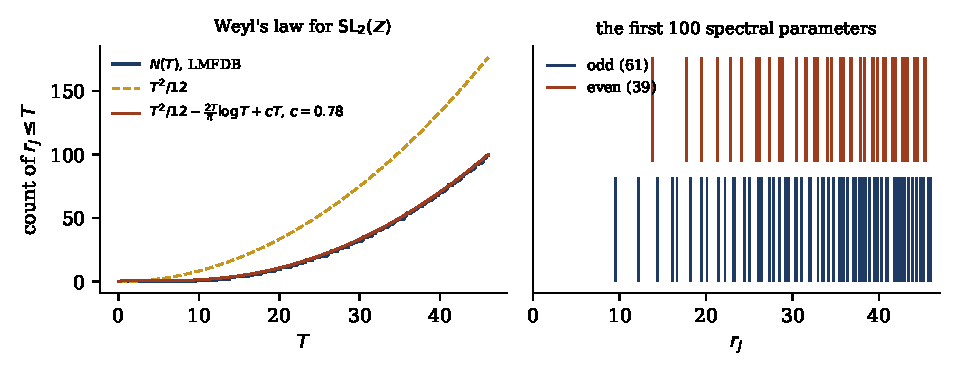
\includegraphics[width=\textwidth]{figs/maass_spectrum.pdf}
\caption{The cuspidal spectrum of $\SL_2(\Z)$. Left: the counting function $N(T)$ of the first hundred spectral parameters against $T^2/12$ and against Weyl's law with its logarithmic term and a fitted linear term. Right: the spectral parameters themselves, odd forms below and even forms above.}\label{fig:msspectrum}
\end{figure}

The Hecke operators $T_n$ commute with $\Delta$ and with each other, so the cusp forms can be taken to be Hecke eigenforms, $T_nu_j=\lambda_j(n)u_j$, with Fourier expansions $u_j(z)=\sum_{n\ne0}\rho_j(n)\sqrt y\,K_{ir_j}(2\pi|n|y)e^{2\pi inx}$ and $\rho_j(n)=\rho_j(1)\lambda_j(n)$ for $n\ge1$. The $L$ function $L(s,u_j)=\sum_{n\ge1}\lambda_j(n)n^{-s}$ has the Euler product $\prod_p(1-\lambda_j(p)p^{-s}+p^{-2s})^{-1}$, Satake parameters $\alpha_p,\alpha_p^{-1}$ with $\alpha_p+\alpha_p^{-1}=\lambda_j(p)$, and the completed function
\[
\Lambda(s,u_j)=\Gamma_\R(s+\epsilon_j+ir_j)\Gamma_\R(s+\epsilon_j-ir_j)L(s,u_j)=(-1)^{\epsilon_j}\Lambda(1-s,u_j),
\]
$\epsilon_j\in\{0,1\}$ the parity, is entire. In the normalisation of Section~\ref{sec:10bcompletion} the archimedean parameters are $\mu=\epsilon_j\pm ir_j$, and $u_j$ generates a cuspidal automorphic representation of $\GL_2(\A_\Q)$, so Theorem~\ref{thm:10bmain} applies: GRH for $L(s,u_j)$ is equivalent to $\Xi_{u_j}(0)/\Xi_{u_j}(\sqrt\lambda)$ being a GGC transform, and Theorem~\ref{thm:10dshift} gives the Thorin representation at every basepoint $\alpha\ge1$ unconditionally.

Two conjectures govern the Maass side and both are statements about the Thorin framework. The \emph{Ramanujan conjecture}\index{Ramanujan conjecture!for Maass forms} for Maass forms is $|\lambda_j(p)|\le2$, that is $|\alpha_p|=1$; for holomorphic forms this is Deligne's theorem, for Maass forms the best known bound is Kim and Sarnak's $|\alpha_p|\le p^{7/64}$ \cite{kimsarnak2003}. \emph{Selberg's eigenvalue conjecture}\index{Selberg's eigenvalue conjecture} is that $\lambda_1\ge\frac14$ for every congruence subgroup, that is that no $r_j$ is imaginary; it is the archimedean Ramanujan conjecture, and Kim and Sarnak's bound gives $\lambda_1\ge\frac14-(\frac7{64})^2=\frac{975}{4096}$. For $\SL_2(\Z)$ itself $\lambda_1=91.14$ and the conjecture is trivially true; the content is in the groups $\Gamma_0(N)$ and $\Gamma(N)$ as $N$ grows.

\begin{corollary}[Ramanujan at $p$ is local Thorin positivity]\label{cor:msramanujan}
Let $u$ be a Hecke Maass eigenform and $p$ a prime. The function
\[
\lambda\mapsto\frac{2-\lambda(p)}{p^{\sqrt\lambda}+p^{-\sqrt\lambda}-\lambda(p)}=(2-\lambda(p))\,p^{-\sqrt\lambda}L_p(\sqrt\lambda,u),
\]
where $L_p(s,u)=(1-\lambda(p)p^{-s}+p^{-2s})^{-1}$ is the Euler factor,
is the Laplace transform of a probability law on $[0,\infty)$ if and only if $-2\le\lambda(p)<2$, in which case the law is the GGC with Thorin comb $\sum_{k\in\Z}\delta_{t_k}$, $t_k=((\theta_p+2\pi k)/\log p)^2$, $\lambda(p)=2\cos\theta_p$. In particular the Ramanujan conjecture at $p$ (with $\lambda(p)\ne2$) holds if and only if the local factor of $u$ at $p$ is a GGC transform in the variable $\sqrt\lambda$.
\end{corollary}

\begin{proof}
$L_p(s,u)^{-1}=1-\lambda(p)p^{-s}+p^{-2s}=p^{-s}(p^s+p^{-s}-\lambda(p))$, so the displayed function is $f_x$ of Theorem~\ref{thm:10clocal} with $x=\lambda(p)$ and $L=\log p$.
\end{proof}

For holomorphic forms the corollary is a theorem at every $p$, by Deligne; for Maass forms it is known only that $\lambda(p)\in[-p^{7/64}-p^{-7/64},p^{7/64}+p^{-7/64}]$, and whether every local factor of every Maass form is a GGC transform is the Ramanujan conjecture itself. Numerically every Hecke eigenvalue ever computed for a Maass form satisfies the bound.

\section{Brownian motion and the heat kernel}\label{sec:msbm}

Brownian motion on $\mathbb H$ is the diffusion with generator $-\Delta=y^2(\partial_x^2+\partial_y^2)$, so that its transition density solves $\partial_tu=-\Delta u$; it is the standard Brownian motion of the metric run at twice the usual speed, which is the convention that makes the heat kernel $e^{-t\Delta}$. In coordinates it solves
\[
dx_t=\sqrt2\,y_t\,dB^1_t,\qquad d\log y_t=\sqrt2\,dB^2_t-dt,
\]
so that $\log y$ is a Brownian motion with drift $-1$ and the process drifts towards the real axis in the half plane, while on $X$ the identification by $\Gamma$ returns it from the cusp. The heat kernel on $\mathbb H$ depends only on the distance $\rho=d(z,w)$ and is (McKean \cite{mckean1972})
\begin{equation}\label{eq:msmckean}
p_t(\rho)=\frac{\sqrt2\,e^{-t/4}}{(4\pi t)^{3/2}}\int_\rho^\infty\frac{s\,e^{-s^2/4t}}{\sqrt{\cosh s-\cosh\rho}}\,ds ,
\end{equation}
with $p_t(0)\sim(4\pi t)^{-1}$ as $t\to0$, the Euclidean value in two dimensions, $p_t(0)\sim\sqrt\pi e^{-t/4}/(8t^{3/2})$ as $t\to\infty$ (Figure~\ref{fig:msheat}), and $p_t(\rho)\asymp t^{-3/2}e^{-t/4-\rho^2/4t-\rho/2}$ up to polynomial factors in $\rho$ and $t$ at large $t$ and $\rho$, the factor $e^{-t/4}$ being the bottom of the spectrum of $\Delta$ on $\mathbb H$. The heat kernel on $X$ is the sum over the group,
\begin{equation}\label{eq:msimages}
K_t(z,w)=\sum_{\gamma\in\bar\Gamma}p_t(d(z,\gamma w)),\qquad\bar\Gamma=\Gamma/\{\pm1\},
\end{equation}
and has the spectral expansion
\begin{equation}\label{eq:msspectral}
\begin{split}
K_t(z,w)={}&\frac3\pi+\sum_{j\ge1}e^{-t\lambda_j}u_j(z)\overline{u_j(w)}\\
&+\frac1{4\pi}\int_{-\infty}^\infty e^{-t(\frac14+r^2)}E(z,\tfrac12+ir)\overline{E(w,\tfrac12+ir)}\,dr .
\end{split}
\end{equation}

\begin{figure}[t]
\centering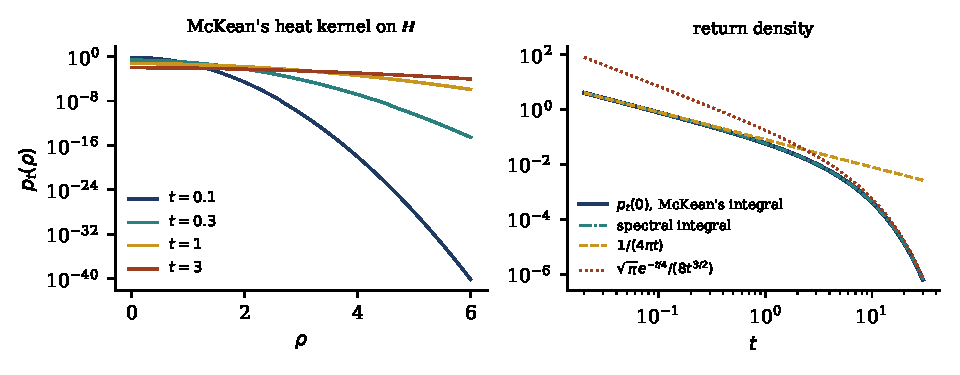
\includegraphics[width=\textwidth]{figs/maass_heat.pdf}
\caption{McKean's heat kernel on $\mathbb H$. Left: $p_t(\rho)$ as a function of the distance $\rho$ for four values of $t$. Right: the return density $p_t(0)$ from \eqref{eq:msmckean} and from the spectral integral $\frac1{4\pi}\int_{\R}e^{-t(1/4+r^2)}r\tanh(\pi r)\,dr$, which agree to $10^{-4}$, between the small time asymptote $1/(4\pi t)$ and the large time asymptote $\sqrt\pi e^{-t/4}/(8t^{3/2})$, whose exponential rate $\frac14$ is the bottom of the spectrum.}\label{fig:msheat}
\end{figure}

\begin{proposition}[Brownian motion on $X$]\label{prop:msergodic}
Brownian motion on $X$ is a positive recurrent diffusion with invariant probability $\frac3\pi d\mu$, and for every $f\in L^1(X,\mu)$, $\frac1T\int_0^Tf(B_s)\,ds\to\frac3\pi\int_Xf\,d\mu$ almost surely. The law of $B_t$ started anywhere converges to $\frac3\pi d\mu$ in total variation, at the rate $e^{-t\lambda_1}$ in $L^2$ with $\lambda_1=91.14$ for the cuspidal part, and at the rate of the continuous spectrum, $e^{-t/4}$ up to a power of $t$, for the Eisenstein part, which is the time it takes the process to come back from the cusp.
\end{proposition}

\begin{proof}
Positive recurrence follows from finiteness of the area and the spectral gap of $\Delta$ on cusp forms together with the explicit form of the continuous spectrum: $\int_XK_t(z,w)f(w)\,d\mu(w)-\frac3\pi\int f\,d\mu$ is bounded in $L^2$ by $e^{-t\lambda_1}\|f\|_2$ for the cuspidal projection and by $e^{-t/4}$ times a power of $t$ for the Eisenstein projection, from \eqref{eq:msspectral}. The ergodic theorem is Birkhoff's for a positive recurrent diffusion.
\end{proof}

The Euler scheme for the stochastic differential equation, with step $10^{-3}$, each step followed by reduction to $F$, gives for $64$ paths run to time $2\cdot10^4$ the time fractions $\Prob(y>1)=0.9551$, $\Prob(y>2)=0.4784$, $\Prob(y>4)=0.2397$, $\Prob(y>8)=0.1201$ against $3/(\pi Y)=0.9549$, $0.4775$, $0.2387$, $0.1194$, and the empirical density of $y$ on $[1,32]$ agrees with $3/(\pi y^2)$ to within $1.1$ percent in every one of twenty logarithmic bins (Figure~\ref{fig:msbm}). The time average of $y^{-1}\mathsf 1_{y\ge1}$ is $0.4769$ against $3/2\pi=0.4775$.

\begin{figure}[t]
\centering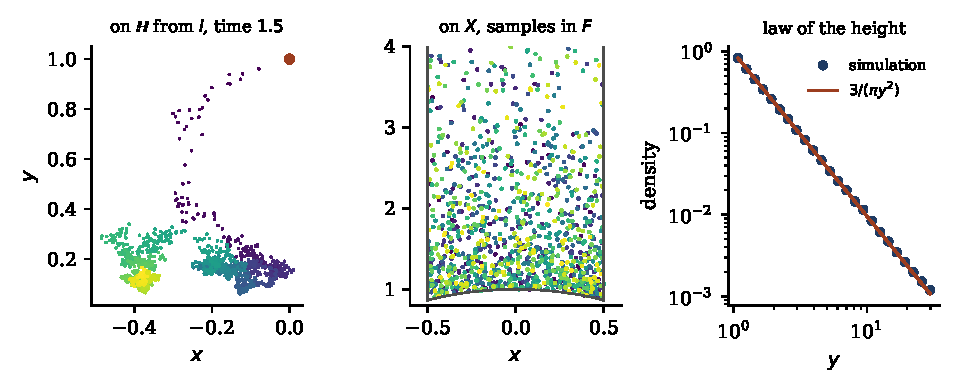
\includegraphics[width=\textwidth]{figs/maass_bm.pdf}
\caption{Brownian motion on the modular surface. Left: a path of the hyperbolic Brownian motion in $\mathbb H$ started at $i$, run to time $1.5$; the drift of $\log y$ carries it towards the real axis. Middle: the process on $X$, every fiftieth sample point in the fundamental domain, coloured by time, filling the domain according to the hyperbolic area. Right: the empirical law of the height $y$ along the path against the density $3/(\pi y^2)$ of the normalised hyperbolic area for $y\ge1$.}\label{fig:msbm}
\end{figure}

\section{The Selberg trace formula as a heat trace}\label{sec:msstf}

For a compact quotient the trace of the heat kernel is both a spectral and a geometric sum, and that is the trace formula. Let $\Gamma$ be a discrete subgroup of $\SL_2(\R)$ acting without fixed points with compact quotient $X_\Gamma$ of genus $g\ge2$, area $4\pi(g-1)$, and Laplace eigenvalues $0=\lambda_0<\lambda_1\le\cdots$, $\lambda_j=\frac14+r_j^2$. Every nontrivial conjugacy class in $\Gamma$ is hyperbolic and is a power $P^k$ of a primitive class $P$, which corresponds to a primitive closed geodesic of length $\ell(P)$; put $N(P)=e^{\ell(P)}$, the norm.

\begin{theorem}[Selberg \cite{selberg1956}; heat kernel form]\label{thm:msstf}
For every $t>0$,
\begin{equation}\label{eq:msstf}
\begin{split}
\sum_{j\ge0}e^{-t\lambda_j}={}&\frac{\operatorname{area}(X_\Gamma)}{4\pi}\int_{-\infty}^\infty e^{-t(\frac14+r^2)}\,r\tanh(\pi r)\,dr\\
&+\sum_P\sum_{k\ge1}\frac{\ell(P)}{2\sinh(k\ell(P)/2)}\,\frac{e^{-t/4}e^{-(k\ell(P))^2/4t}}{\sqrt{4\pi t}} .
\end{split}
\end{equation}
\end{theorem}

This is the general trace formula
\[
\sum_jh(r_j)=\frac{\operatorname{area}}{4\pi}\int h(r)\,r\tanh(\pi r)\,dr+\sum_{P,k}\frac{\ell(P)}{2\sinh(k\ell(P)/2)}\,g(k\ell(P)),
\]
with $g(u)=\frac1{2\pi}\int h(r)e^{-iru}\,dr$, applied to $h(r)=e^{-t(1/4+r^2)}$, for which $g(u)=e^{-t/4}e^{-u^2/4t}/\sqrt{4\pi t}$. For the modular surface the same identity holds with elliptic terms for the two elliptic points, parabolic terms for the cusp, and the spectral side carrying the continuous spectrum through the scattering determinant; the statement is in Hejhal \cite{hejhal1983} and Iwaniec \cite{iwaniec2002}, and the structure is the same.

The probabilistic reading is McKean's \cite{mckean1972}, and the book's dictionary makes it exact. By \eqref{eq:msimages} and \eqref{eq:msspectral},
\[
\sum_je^{-t\lambda_j}=\int_{X_\Gamma}K_t(z,z)\,d\mu(z)=\int_{X_\Gamma}\sum_\gamma p_t(d(z,\gamma z))\,d\mu(z).
\] The term $\gamma=1$ is $\operatorname{area}\cdot p_t(0)$, the return density of free Brownian motion on $\mathbb H$ integrated over the surface, and \eqref{eq:msmckean} integrated against $\tanh$ is the statement $p_t(0)=\frac1{4\pi}\int e^{-t(1/4+r^2)}r\tanh(\pi r)\,dr$, the spectral density of $\Delta$ on $\mathbb H$. The terms $\gamma\sim P^k$ collect, for each $z$, the density at $z$ of Brownian paths from $z$ that return to $z$ in the free homotopy class of the closed geodesic $P^k$: a path from $z$ to $\gamma z$ in $\mathbb H$ is a loop on $X_\Gamma$ in the class of $\gamma$. Integrating over a fundamental domain of the centraliser of $P$ gives the factor $\ell(P)/(2\sinh(k\ell(P)/2))$, and $g(k\ell(P))$ is the one dimensional Gaussian density at distance $k\ell(P)$ with the spectral shift $e^{-t/4}$. So \eqref{eq:msstf} says: the total return probability of Brownian motion on $X_\Gamma$ equals the free return probability plus the sum over closed geodesics of the probability of returning around that geodesic. Compare the Galois heat trace of Definition~\ref{def:recipheat},
\[
\begin{split}
\mathcal W_\rho(x)={}&\frac1{4\pi}\int e^{-xr^2}\Bigl(\log N_\rho+2\operatorname{Re}\frac{\gamma'}\gamma(\tfrac12+ir,\rho)\Bigr)dr\\
&-\frac1{2\sqrt{\pi x}}\sum_{n\ge2}\frac{\Lambda_\rho(n)}{\sqrt n}\,e^{-(\log n)^2/4x},
\end{split}
\]
which equals $\frac12\sum e^{-x\gamma^2}$ over the zeros $\frac12+i\gamma$ (Theorem~\ref{thm:recipcm}). The two formulas have the same three parts: a spectral sum ($e^{-tr_j^2}$ over eigenvalues, $e^{-x\gamma^2}$ over zeros), an archimedean integral ($r\tanh\pi r$, $\gamma'/\gamma$), and a sum over primes ($\log N(P)=\ell(P)$ with the Gaussian $e^{-(k\ell)^2/4t}$, $\Lambda(n)=\log p$ with $e^{-(\log n)^2/4x}$). The one difference is the sign of the prime sum, and it is explained by the Selberg zeta function below: $Z$ is built like $1/\zeta$, so its logarithmic coefficients are $-\ell(P)$ where those of $\zeta$ are $+\log p$.

\begin{theorem}[Selberg's conjecture as complete monotonicity; this book]\label{thm:mscm}
Let $\Gamma$ be a congruence subgroup of $\SL_2(\Z)$ and $\Theta_\Gamma(t)=\sum_{j\ge1}e^{-t\lambda_j}$ the heat trace over the Maass cusp forms, $\lambda_j=\frac14+r_j^2$.
\begin{enumerate}
\item[(i)] $e^{t/4}\Theta_\Gamma(t)=\sum_je^{-tr_j^2}$ is completely monotone on $(0,\infty)$ if and only if $\lambda_j\ge\frac14$ for every $j$, that is if and only if Selberg's eigenvalue conjecture holds for $\Gamma$; in that case its Bernstein measure is $\sum_j\delta_{r_j^2}$.
\item[(ii)] Unconditionally, $e^{t(\frac14-(7/64)^2)}\Theta_\Gamma(t)$ is completely monotone.
\item[(iii)] For $\Gamma=\SL_2(\Z)$, (i) holds, and $\sum_je^{-tr_j^2}\sim\frac1{12t}$ as $t\to0$.
\item[(iv)] The measure $\sum_j\delta_{r_j^2}$ is not a Thorin measure: $\sum_jr_j^{-2}=\infty$.
\end{enumerate}
\end{theorem}

\begin{proof}
(i) By Weyl's law the series converges for $t>0$. If every $r_j^2\ge0$ the function is a Laplace transform of a positive measure, hence completely monotone by Bernstein's theorem, with the stated Bernstein measure by uniqueness. If some $\lambda_j<\frac14$ then $r_j^2<0$ and the corresponding term grows exponentially, so the function is not bounded as $t\to\infty$, while a completely monotone function is decreasing. (ii) is (i) applied with the shift $\frac14-(\frac7{64})^2$, since $\lambda_j\ge\frac{975}{4096}$ by Kim and Sarnak. (iii) The first statement is $\lambda_1=91.14$; the asymptotic is Karamata's Tauberian theorem applied to \eqref{eq:msweyl}, or directly the identity term of the trace formula, $\frac{\operatorname{area}}{4\pi}\int e^{-tr^2}r\tanh(\pi r)\,dr\sim\frac{\operatorname{area}}{4\pi t}=\frac1{12t}$. (iv) By Weyl's law for $\Gamma$, $N(T)\sim\frac{\operatorname{area}}{4\pi}T^2$, of which \eqref{eq:msweyl} is the case $\SL_2(\Z)$, the sum $\sum_jr_j^{-2}=\int_1^\infty T^{-2}\,dN(T)$ diverges like $\frac{\operatorname{area}}{2\pi}\log T$ (like $\frac16\log T$ for $\SL_2(\Z)$), so the second integrability condition of Definition~\ref{def:ch10ggc}, $\int_{(1,\infty)}t^{-1}\tau(dt)<\infty$, fails.
\end{proof}

Theorem~\ref{thm:mscm} is Theorem~\ref{thm:recipcm} with eigenvalues for zeros, and on the Maass side much of the analogue of the Riemann hypothesis comes free: the Laplacian is self adjoint and the Hecke operators commute with it, so every $r_j^2$ is real and the only possible exceptions are finitely many eigenvalues $\lambda_j<\frac14$, which is the whole content of the Maass side being spectral. Selberg's conjecture, that there are none, is open in general; it holds for $\SL_2(\Z)$, which gives part (iii), and part (ii) is what the bound of Kim and Sarnak gives for every congruence subgroup. Part (iv) is the limit of the analogy. The zeros of an $L$ function of degree $n$ have counting function $\frac{nT}{2\pi}\log T$, a one dimensional spectrum, and $\sum\gamma^{-2}$ converges, so Theorem~\ref{thm:10bmain} can place them in a Thorin measure. The eigenvalues of a surface have a two dimensional count, $\sum r_j^{-2}$ diverges logarithmically, and the function $\prod_j(1+\lambda/r_j^2)$ does not converge; the Selberg zeta function is of order two, and no GGC has it for a Laplace transform. The heat trace is the right object, and the Thorin framework enters, as the next section shows, through the Euler product and not through the spectrum.

\section{Closed geodesics as primes}\label{sec:msgeodesics}

The Selberg zeta function\index{Selberg zeta function} of $\Gamma$ is
\[
Z(s)=\prod_P\prod_{k\ge0}\bigl(1-N(P)^{-s-k}\bigr),\qquad\operatorname{Re}s>1,
\]
the product over primitive hyperbolic classes. It continues to an entire function of order two (compact case; meromorphic for $\SL_2(\Z)$), with zeros at $s_j=\frac12\pm ir_j$ for each eigenvalue $\lambda_j=\frac14+r_j^2$, a simple zero at $s=1$ from $\lambda_0=0$, and zeros at the nonpositive integers of multiplicity growing linearly; for $\SL_2(\Z)$ there are in addition zeros at $s=\rho/2$ for the nontrivial zeros $\rho$ of $\zeta$, coming from the scattering determinant $\varphi(s)=\sqrt\pi\,\Gamma(s-\frac12)\zeta(2s-1)/(\Gamma(s)\zeta(2s))$. For a congruence subgroup the zeros $s_j$ lie on $\operatorname{Re}s=\frac12$ if and only if Selberg's eigenvalue conjecture holds, and for $\SL_2(\Z)$ the additional zeros $\rho/2$ lie on $\operatorname{Re}s=\frac14$ if and only if the Riemann hypothesis holds; a compact surface may have eigenvalues below $\frac14$, and then $Z$ has real zeros in $(\frac12,1)$.

The ratio
\begin{equation}\label{eq:msR}
R(s)=\frac{Z(s+1)}{Z(s)}=\prod_P\bigl(1-N(P)^{-s}\bigr)^{-1}=\sum_{\mathfrak n}N(\mathfrak n)^{-s}
\end{equation}
is an Euler product of the shape of $\zeta$, the sum running over the free abelian monoid generated by the primitive geodesics, whose elements we call \emph{geodesic integers}\index{geodesic integer} and whose norms are multiplicative. The prime geodesic theorem,
\[
\pi_\Gamma(x)=\#\{P:\ N(P)\le x\}=\operatorname{li}(x)+O(x^{3/4+\epsilon})
\]
for the modular surface, is due to Huber and Selberg for compact surfaces, where the terms $\operatorname{li}(x^{s_j})$ of the eigenvalues $\lambda_j<\frac14$ are added, and to Sarnak for $\SL_2(\Z)$ \cite{sarnak1982}, where the exponent has since been lowered to $\frac{25}{36}$ \cite{soundararajanyoung2013}; the primitive geodesics of $\SL_2(\Z)$ correspond to the narrow classes of primitive binary quadratic forms of positive nonsquare discriminant $d$, with $N(P)=\epsilon_d^2$ for the smallest unit $\epsilon_d>1$ of norm $+1$ in the order of discriminant $d$, so that $\pi_\Gamma(x)=\sum_{\epsilon_d\le\sqrt x}h^+(d)$ and the theorem is a statement about class numbers of indefinite forms. Enumerating the discriminants to $4\cdot10^6$ with their units and class numbers gives $78441$ primitive geodesics of norm at most $10^6$, against $\operatorname{li}(10^6)=78628$, ratio $0.9976$, and $\sum_{N(P)^k\le x}\ell(P)=0.9991x$ at $x=10^6$ (Figure~\ref{fig:msgeodesics}, left); the shortest geodesic has $N(P)=\varphi^4=6.854$, $\varphi$ the golden ratio, from the discriminant $5$, and the second shortest has norm $13.93$ with multiplicity two, from the discriminant $12$ whose order has no unit of norm $-1$.

\begin{figure}[t]
\centering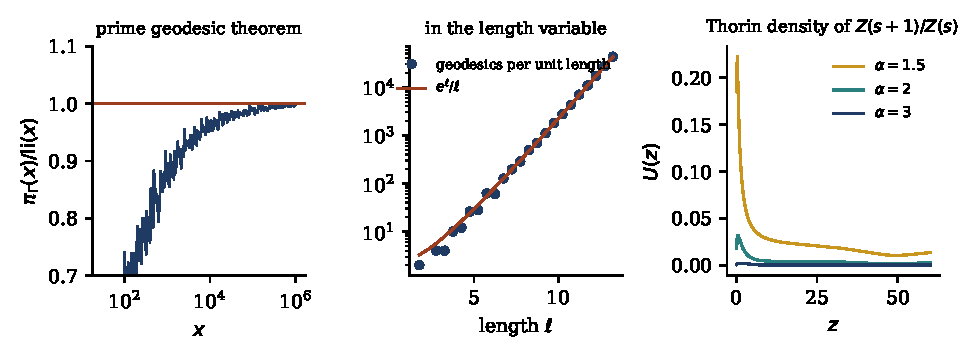
\includegraphics[width=\textwidth]{figs/maass_geodesics.pdf}
\caption{Left: the prime geodesic theorem on the modular surface, $\pi_\Gamma(x)/\operatorname{li}(x)$ for $x\le10^6$ from the class numbers and units of the $2\cdot10^6$ discriminants below $4\cdot10^6$. Middle: the number of primitive geodesics per unit length against $e^\ell/\ell$, the prime geodesic theorem in the length variable. Right: the Thorin density $U(z)$ of the geodesic Euler product $Z(s+1)/Z(s)$ at the basepoints $\alpha=1.5$, $2$ and $3$, from Theorem~\ref{thm:msthorin}; it is positive and integrable, and at $\alpha=2$ its integral against $\log(1+z/t)$ reproduces $\log(R(2)/R(2+\sqrt z))$ to between $10^{-7}$ and $10^{-5}$.}\label{fig:msgeodesics}
\end{figure}

The eigenvalues are visible in the geodesic count. The explicit formula for the modular surface, which is the trace formula with a sharp cutoff for $h$, gives $\psi_\Gamma(x)=\sum_{N(P)^k\le x}\ell(P)=x+\sum_jx^{s_j}/s_j+\cdots$ with $s_j=\frac12\pm ir_j$, so that $(\psi_\Gamma(x)-x)/\sqrt x$ is, up to smaller terms, the almost periodic function $\sum_j2\operatorname{Re}(x^{ir_j}/s_j)$ of $u=\log x$, with frequencies the $r_j$ and amplitudes about $2/r_j$. Figure~\ref{fig:mszeta} shows this function on $50\le x\le10^6$ and its periodogram in $u$: the largest peak below $r=19$ is at $r=9.53$, the first eigenvalue, and the next peaks are at $12.13$, $14.11$ and $16.27$, where the resolution $2\pi/\log(2\cdot10^4)\approx0.6$ of a window of length $\log(2\cdot10^4)$ does not separate the pairs $13.78$, $14.36$ and $16.14$, $16.64$. This is the prime side hearing the spectral side, Weil's explicit formula read backwards, and it is the arithmetic content of Theorem~\ref{thm:msstf}. The right panel of the figure shows the two terms of the heat trace formula as functions of $t$, the identity term $\sim1/(12t)$ at small $t$ and the geodesic sum, which is $O(e^{-\ell_1^2/4t})$ at small $t$ and overtakes the identity term only for $t$ of order one, where the whole trace is dominated by $\lambda_0=0$.

\begin{figure}[t]
\centering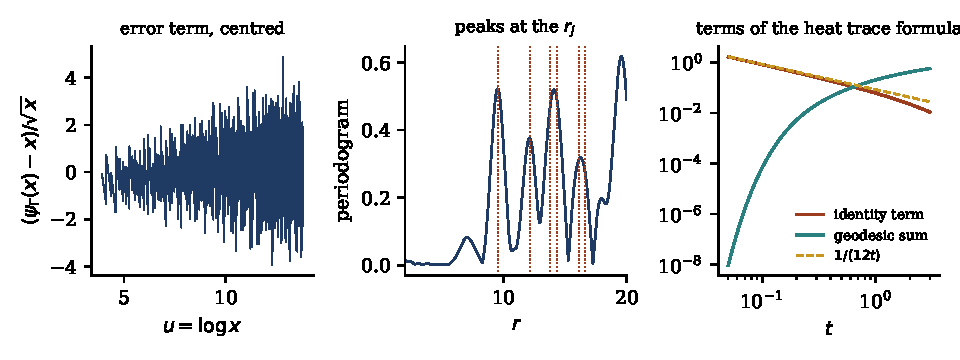
\includegraphics[width=\textwidth]{figs/maass_zeta.pdf}
\caption{The spectrum in the geodesics. Left: the error term $(\psi_\Gamma(x)-x)/\sqrt x$ of the prime geodesic theorem, centred, as a function of $u=\log x$. Middle: its periodogram in $u$, with the first six eigenvalue parameters $r_j$ marked; the peak at $9.53$ is the first Maass form. Right: the identity term and the geodesic sum of the heat trace formula \eqref{eq:msstf} for the modular surface as functions of $t$.}\label{fig:mszeta}
\end{figure}

With these facts the geodesics are a Beurling system of generalised primes satisfying the prime number theorem, and the two tools of Chapters~\ref{ch:10d} and \ref{ch:pd} that use nothing else apply to them.

\begin{theorem}[Thorin representation of the geodesic Euler product; this book]\label{thm:msthorin}
Let $\alpha>1$. Then for $\lambda>0$
\[
\frac{R(\alpha)}{R(\alpha+\sqrt\lambda)}=e^{-b\sqrt\lambda}\,\E e^{-\lambda H},\qquad b=\frac{R'}{R}(\alpha)=-\sum_{P,k}\ell(P)N(P)^{-k\alpha},
\]
where $H$ is a GGC with drift zero and Thorin density
\[
U(z)=\frac1{2\pi\sqrt z}\sum_P\sum_{k\ge1}\ell(P)\,N(P)^{-k\alpha}\,2\sin^2\Bigl(\frac{k\ell(P)\sqrt z}2\Bigr)\ge0,
\]
equal to $(\operatorname{Re}(R'/R)(\alpha+i\sqrt z)-b)/(2\pi\sqrt z)$.
The same holds for the modular surface, and for the Dedekind zeta function of any number field and the Rankin Selberg $L$ function $L(s,\pi\times\tilde\pi)$ of an automorphic representation and its contragredient, whose logarithmic coefficients $|a_\pi(p^k)|^2\log p$ are nonnegative, with the primes of the field or the Rankin Selberg coefficients in place of the geodesics.
\end{theorem}

\begin{proof}
$\log R(\alpha+s)=\sum_{P,k}k^{-1}N(P)^{-k\alpha}e^{-sk\ell(P)}$, so \eqref{eq:10dlk} holds with the positive measure $\nu=\sum_{P,k}\ell(P)N(P)^{-k\alpha}\delta_{k\ell(P)}$, which is finite by the prime geodesic theorem, and Lemma~\ref{lem:10dsin2} applies. The formula for $U$ is \eqref{eq:10dU}.
\end{proof}

At $\alpha=2$ the density is dominated by the shortest geodesics and is shown in Figure~\ref{fig:msgeodesics}; the identity
\[
\log\frac{R(\alpha)}{R(\alpha+\sqrt z)}=-b\sqrt z-\int_0^\infty\log\Bigl(1+\frac zt\Bigr)U(t)\,dt
\]
checks to $9\cdot10^{-8}$, $5\cdot10^{-7}$ and $4\cdot10^{-6}$ at $z=\frac12,2,10$, the residual being the numerical integration. The drift $b$ is negative, so $R(\alpha)/R(\alpha+\sqrt\lambda)=e^{|b|\sqrt\lambda}\E e^{-\lambda H}$ increases from $1$ to $R(\alpha)$ and is the transform of $H$ divided by the transform $e^{-|b|\sqrt\lambda}$ of a one half stable law, exactly as for $\zeta$ in Lemma~\ref{lem:10dsin2}. Theorem~\ref{thm:msthorin} is unconditional for every basepoint $\alpha>1$, and what it does not give is the representation at $\alpha=\frac12+a$: there the poles of $R$ at the spectrum $s_j$ contribute positive Cauchy terms to the Thorin density and its zeros at $s_j-1$ contribute negative ones, and because of Theorem~\ref{thm:mscm}(iv) the two series are each divergent; the trivial poles of $R$ at the nonpositive integers, of constant multiplicity, supply the compensating logarithmic growth. Whether $R(\frac12+a)/R(\frac12+a+\sqrt\lambda)$, with the pole at $s=1$ removed, is a GGC transform for small $a>0$ is Open Problem~\ref{op:mscentre}.

\begin{theorem}[random geodesic integers are Poisson Dirichlet; this book]\label{thm:mspd}
Let $\mathfrak n_\sigma$ be the random geodesic integer with $\Prob(\mathfrak n_\sigma=\mathfrak n)=N(\mathfrak n)^{-\sigma}/R(\sigma)$, $\sigma>1$. Its exponents $e_P$ are independent geometric variables with $\Prob(e_P\ge k)=N(P)^{-k\sigma}$, and as $\sigma\downarrow1$: the point process of rescaled sizes $(\sigma-1)e_P\ell(P)$ converges to the Poisson process with intensity $x^{-1}e^{-x}dx$, the Gamma process; the ranked normalised sizes $e_P\ell(P)/\log N(\mathfrak n_\sigma)$ converge to $\mathrm{PD}(1)$; the largest primitive geodesic factor has Dickman's law in the limit; and the number of distinct primitive factors is asymptotically normal with mean and variance $\log\frac1{\sigma-1}$.
\end{theorem}

\begin{proof}
The proof of Theorem~\ref{thm:recipgammaproc}, through Lemma~\ref{lem:recipnu}, uses of the primes only two things: $\sum_{N(P)\le x}\ell(P)\sim x$, which is the prime geodesic theorem by partial summation, and $\sum_PN(P)^{-2}<\infty$. Both hold for the geodesics, and the labels may be taken trivial. The Poisson Dirichlet limit, Dickman's law and the normal law for the number of factors then follow exactly as in Theorems~\ref{thm:pdbillingsley}, \ref{thm:pderdoskac} and \ref{thm:pdtheta} with $\theta=1$, the order of the pole of $R$ at $s=1$, which is simple because the zero of $Z$ at $s=1$ is simple ($\lambda_0=0$ has multiplicity one on a connected surface) and $Z(2)\ne0$.
\end{proof}

The uniform analogue, a geodesic integer chosen uniformly among those of norm at most $x$, obeys the same limit laws with $\log x$ in place of $\log\frac1{\sigma-1}$, since the arguments of Chapter~\ref{ch:pd} use only the prime number theorem with a power saving in the error term, which the prime geodesic theorem supplies. What is missing is a Chebotarev theorem: the geodesics carry natural labels, the discriminant $d$ modulo $q$, the type of the order, the sign of the norm of the fundamental unit, and the densities of these labels in the ordering by $N(P)$ would be the base measure of a Dirichlet process of geodesics. Some are known. Sarnak \cite{sarnakreciprocal2007} showed that the reciprocal geodesics, those conjugate to their own inverse in $\mathrm{PSL}_2(\Z)$, which correspond to the forms $f$ equivalent to $-f$, are only about $\frac38\sqrt x$ in number with norm below $x$, so they form a class of density zero and the Dirichlet process does not see them; the densities of the discriminant classes modulo $q$ are Open Problem~\ref{op:mschebotarev}.

\section{Eigenvalue one quarter and parity}\label{sec:msquarter}

A Maass form with $\lambda=\frac14$ has $r=0$ and gamma factor $\Gamma_\R(s+\epsilon)^2$. A two dimensional Artin representation $\rho$ is even when $\det\rho(c)=1$ for complex conjugation $c$, so that $\rho(c)=I$ or $\rho(c)=-I$, and its gamma factor is then $\Gamma_\R(s)^2$ or $\Gamma_\R(s+1)^2$ respectively; an odd representation, $\det\rho(c)=-1$, has $\Gamma_\R(s)\Gamma_\R(s+1)=\Gamma_\C(s)$, the gamma factor of a holomorphic form of weight one. So the Maass forms that can be Galois are those of eigenvalue exactly $\frac14$, of parity $\epsilon$ with $\rho(c)=(-1)^\epsilon I$, and the case $\rho(c)=I$ is exactly the case in which the Galois heat trace of Definition~\ref{def:recipheat} is computed with the Maass gamma factor $\Gamma_\R(s)^2$.

\begin{theorem}[Maass, Hecke; Langlands, Tunnell]\label{thm:msgalois}
Let $\rho$ be an irreducible two dimensional Artin representation that is even. If $\rho$ is dihedral, tetrahedral or octahedral there is a Maass cusp form $u_\rho$ of eigenvalue $\frac14$ and parity $\epsilon$, $\rho(c)=(-1)^\epsilon I$, on some $\Gamma_0(N)$ with character, with $L(s,\rho)=L(s,u_\rho)$; in the dihedral case $u_\rho$ is one of Maass's original forms, induced from a ray class character of a real quadratic field. If $\rho$ is icosahedral, the existence of $u_\rho$ is open in general. Conversely it is conjectured that every Maass cusp form of eigenvalue $\frac14$ whose Hecke eigenvalues are algebraic integers arises in this way.
\end{theorem}

Theorem~\ref{thm:recipcm} now reads as follows. For a self dual $\rho$ with $\rho(c)=I$ and root number $+1$, the heat trace $\mathcal W_\rho^+$ of Definition~\ref{def:recipheat} computed with the Maass gamma factor $\Gamma_\R(s)^2$ is completely monotone if and only if $\Lambda(s,\rho)$ is entire and GRH holds; and if $\rho$ is odd, so that it has a weight one form, the same function computed with the wrong parity differs by $\Delta(x)=\frac14\E e^{-xC^2}$ with $C$ hyperbolic secant distributed, and under GRH fails to be completely monotone. The difference comes from the gamma factors alone: at $s=\frac12+it$ the reflection formula of $\Gamma'/\Gamma$ gives $\operatorname{Re}\frac d{ds}\log\frac{\Gamma_\R(s+1)}{\Gamma_\R(s)}=\frac\pi2\operatorname{Re}\cot\bigl(\frac\pi4+\frac{i\pi t}2\bigr)=\frac\pi2\operatorname{sech}\pi t$, and $\operatorname{sech}\pi t$ is the density of $C$; under GRH the measure of the function computed with the wrong parity is $\frac12\sum\delta_{\gamma^2}$ less a quarter of the law of $C^2$, which has a positive density on $(0,\infty)$, so it is not positive. The parity of a two dimensional Artin representation is therefore which of two gamma factors makes its heat trace a Laplace transform, and the Maass form of eigenvalue $\frac14$, when it exists, is the object whose heat trace that is. The even icosahedral case is Open Problem~\ref{op:mseven}: there the heat trace is defined from Frobenius traces, its complete monotonicity is equivalent to Artin's conjecture and GRH together, and the Maass form whose existence Artin's conjecture asserts would have eigenvalue exactly $\frac14$ on $\Gamma_0(N)$ for the Artin conductor $N$; to our knowledge no Maass form of eigenvalue exactly $\frac14$ that is not dihedral, tetrahedral or octahedral has been exhibited.

\section{The Eichler Selberg trace formula}\label{sec:mses}

The holomorphic analogue of \eqref{eq:msstf} is the formula for the trace of a Hecke operator on $S_k(\SL_2(\Z))$, which Chapter~\ref{ch:07} uses in the form of Serre's vertical Sato Tate theorem and which is stated here. Let $H(N)$ be the Hurwitz class number, the number of $\SL_2(\Z)$ classes of positive definite binary quadratic forms of discriminant $-N$ weighted by the reciprocal of the order of the automorphism group in $\mathrm{PSL}_2(\Z)$, so that the forms equivalent to $a(x^2+y^2)$ and $a(x^2+xy+y^2)$ count $\frac12$ and $\frac13$, with $H(0)=-\frac1{12}$, and let $P_k(t,n)$ be the coefficient of $X^{k-2}$ in $(1-tX+nX^2)^{-1}$, so that $P_k(t,n)=(\varrho^{k-1}-\bar\varrho^{\,k-1})/(\varrho-\bar\varrho)$ for the roots $\varrho,\bar\varrho$ of $X^2-tX+n$.

\begin{theorem}[Eichler, Selberg \cite{eichler1957,selberg1956}; see Zagier \cite{lang1976,zagier1977}]\label{thm:mses}
For even $k\ge4$ and $n\ge1$,
\[
\tr\bigl(T_n\,|\,S_k(\SL_2(\Z))\bigr)=-\frac12\sum_{t^2\le4n}P_k(t,n)H(4n-t^2)-\frac12\sum_{dd'=n}\min(d,d')^{k-1},
\]
the first sum over all integers $t$ with $t^2\le4n$ and the second over the positive divisors.
\end{theorem}

The formula was checked against the Hecke matrices computed by PARI on $S_k$ for every even $k$ from $12$ to $40$ and every $n\le30$, $450$ cases, without a discrepancy; the first case is $\tr T_2|S_{12}=\tau(2)=-24$, and on $S_{24}$ the two eigenvalues of $T_2$ sum to $1080$.

Its probabilistic reading is the one Chapter~\ref{ch:07} gave the Hecke operators. For $n=p^m$ write $a_p(f)=2p^{(k-1)/2}\cos\theta_p(f)$ for each of the $d_k=\dim S_k$ normalised eigenforms; then $a_{p^m}(f)=p^{m(k-1)/2}U_m(\cos\theta_p(f))$ with $U_m$ the Chebyshev polynomial of the second kind, and Theorem~\ref{thm:mses} is a formula for the empirical moment
\[
\frac1{d_k}\sum_fU_m(\cos\theta_p(f))=\frac{\tr T_{p^m}}{d_k\,p^{m(k-1)/2}} .
\]
The term $t^2=4n$, present only when $m$ is even, contributes $\frac{(k-1)}{12}p^{m(k-2)/2}$ through $H(0)=-\frac1{12}$, and since $d_k\sim\frac k{12}$ this term alone gives the limit $p^{-m/2}$ of the moment as $k\to\infty$, which is $\int U_m(\cos\theta)\,d\mu_p$ for the Plancherel measure $\mu_p$ of the $(p+1)$ regular tree, the Kesten McKay law of Chapter~\ref{ch:07}: the identity term of the trace formula is the return probability of the random walk on the tree, and the class number terms measure the finite graph's departure from the tree. The remaining terms are $o(1)$ in $k$ (Conrey, Duke and Farmer \cite{cdf1997} at level one, Serre \cite{serre1997} in general), which is the vertical Sato Tate theorem, Theorem~\ref{thm:07serre}. For $p=2$ and all $3234$ eigenforms of level one and weight at most $400$ the normalised eigenvalues $a_2(f)/2^{(k-1)/2}$ have moments $1.485$, $3.683$, $10.61$ against $\frac32$, $\frac{15}4$, $\frac{87}8$ for $\mu_2$ and $1$, $2$, $5$ for the Sato Tate law, and Kolmogorov distance $0.0055$ to $\mu_2$ against $0.089$ to Sato Tate (Figure~\ref{fig:msvertical}). The vertical and the horizontal limits differ because at fixed $p$ the eigenvalues see the tree, while at fixed $f$ and $p\to\infty$ the measures $\mu_p$ converge to the semicircle.

\begin{figure}[t]
\centering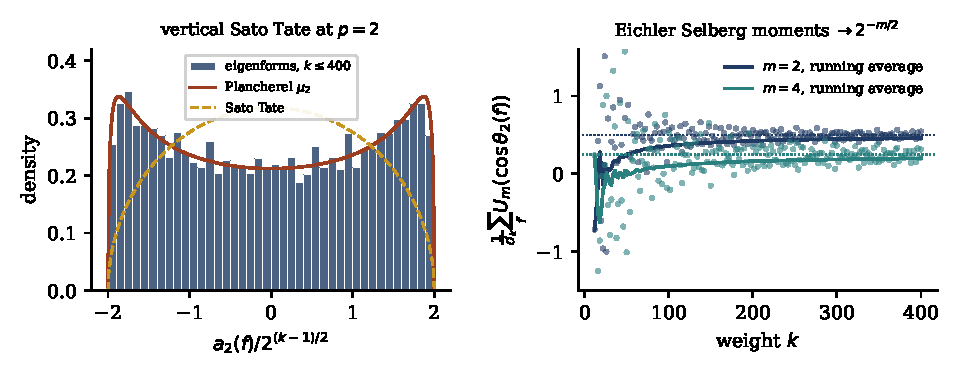
\includegraphics[width=\textwidth]{figs/maass_vertical.pdf}
\caption{Left: Serre's vertical Sato Tate law at $p=2$, the normalised Hecke eigenvalues $a_2(f)/2^{(k-1)/2}$ of the $3234$ level one eigenforms of weight at most $400$ against the Plancherel measure $\mu_2$ of the $3$ regular tree and the Sato Tate law. Right: the empirical moments $\frac1{d_k}\sum_fU_m(\cos\theta_2(f))$ for $m=2$ and $m=4$, computed from the Eichler Selberg formula for every even weight up to $400$ (dots), and their running averages over $k$ (lines), approaching $2^{-m/2}$.}\label{fig:msvertical}
\end{figure}

\section{What this adds to the programme}

The chapter adds the second half of the automorphic spectrum and finds the book's dictionary intact on it: heat trace for explicit formula, eigenvalues for zeros, geodesics for primes, complete monotonicity for the Riemann hypothesis, with Brownian motion on the surface as the probabilistic object that makes the trace formula a statement about return probabilities. It adds two unconditional theorems in the Thorin framework, Theorems~\ref{thm:msthorin} and \ref{thm:mspd}, which are the sine squared lemma and the Poisson Dirichlet theorem for a Beurling system of primes, and one theorem, Theorem~\ref{thm:mscm}, that is the Galois heat trace theorem with the Riemann hypothesis replaced by Selberg's eigenvalue conjecture, and with the complete monotonicity it characterises proved for $\SL_2(\Z)$ and, after the shift of Kim and Sarnak, for every congruence subgroup. It also adds the obstruction of Theorem~\ref{thm:mscm}(iv), which says why the zeros of an $L$ function can be a Thorin measure and the eigenvalues of a surface cannot, and which separates the arithmetic case from the geometric one by a logarithm. Finally it places the even icosahedral problem where it belongs, among the Maass forms of eigenvalue $\frac14$, and shows that the parity of a two dimensional Artin representation is a statement about which gamma factor, holomorphic or Maass, its Galois heat trace wants.

\section{Notes}

Maass introduced his forms in \cite{maass1949} and Selberg the trace formula and the zeta function in \cite{selberg1956}; Hejhal's two volumes \cite{hejhal1976,hejhal1983} and Iwaniec \cite{iwaniec2002} are the references for the noncompact case, and Sarnak's survey \cite{sarnak2003} for the eigenvalue conjecture. McKean's reading of the trace formula through Brownian motion is \cite{mckean1972}; the heat kernel \eqref{eq:msmckean} is there and in Chavel \cite{chavel1984}. The computation of the eigenvalues of $\SL_2(\Z)$ is Hejhal's \cite{hejhal1992}, with rigorous certification by Booker, Str\"ombergsson and Venkatesh \cite{bookerstrombergssonvenkatesh2006}; the values quoted are from the LMFDB \cite{lmfdb}. Weyl's law for $\SL_2(\Z)$ is Selberg's; the lower order terms are in Hejhal. The Kim Sarnak bound is \cite{kimsarnak2003}. The prime geodesic theorem for $\SL_2(\Z)$ and its reading through class numbers is Sarnak \cite{sarnak1982}, reciprocal geodesics are \cite{sarnakreciprocal2007}, and the exponent $\frac{25}{36}$ is Soundararajan and Young \cite{soundararajanyoung2013}. The Eichler Selberg formula is in \cite{eichler1957} and \cite{selberg1956}; the form used is Zagier's, in his appendix to Lang \cite{lang1976} and in \cite{zagier1977}, and the vertical equidistribution is Serre's \cite{serre1997}, with the level one case in Conrey, Duke and Farmer \cite{cdf1997}. Theorems~\ref{thm:mscm}, \ref{thm:msthorin} and \ref{thm:mspd} are new as formulated; their content is Selberg's, Thorin's and Kingman's, assembled through Chapters~\ref{ch:10d}, \ref{ch:recip} and \ref{ch:pd}.

\section{Exercises}

\begin{enumerate}
\item Show that the hyperbolic Brownian motion of Section~\ref{sec:msbm}, started at $i$, has $\E\log y_t=-t$ and that $\log y_t/t\to-1$ almost surely, so that on $\mathbb H$ the process converges to the boundary; explain why on $X$ it does not.
\item Verify from \eqref{eq:msmckean} that $p_t(0)\sim(4\pi t)^{-1}$ as $t\to0$, and that $p_t$ integrates to $1$ over $\mathbb H$.
\item Derive $\pi_\Gamma(x)\sim x/\log x$ from the trace formula with $h(r)=e^{-t(1/4+r^2)}$ as $t\to\infty$, using only $\lambda_0=0$ and $\lambda_1>0$.
\item Show that $R(s)=Z(s+1)/Z(s)$ has a simple pole at $s=1$ with residue $\lim_{s\to1}(s-1)R(s)=Z(2)/Z'(1)$, and compute $Z'(1)$ and $Z(2)$ for the modular surface from the geodesics of norm at most $10^6$.
\item For the Hecke Maass form with $r_1=9.533695$, look up $\lambda(2)$ in the LMFDB, check the Ramanujan bound $|\lambda(2)|\le2$, and write down the Thorin comb of Corollary~\ref{cor:msramanujan}.
\item Prove that the hyperbolic terms of \eqref{eq:msstf} sum to $O(t^{-1/2}e^{-\ell_1^2/4t})$ as $t\to0$, $\ell_1$ the length of the shortest geodesic, so that the identity term alone gives Weyl's law.
\item Using Theorem~\ref{thm:mses}, find all pairs $(k,p)$ with $k\le40$ and $p\le30$ for which $\tr T_p|S_k=0$.
\item Compute $\int U_m(\cos\theta)\,d\mu_p$ for all $m$ and check that the even moments are $p^{-m/2}$.
\end{enumerate}

\section{Open problems}

\begin{problem}[the Thorin representation at the centre]\label{op:mscentre}
Let $R(s)=Z(s+1)/Z(s)$ for a compact surface, and $R^*(s)=(s-1)R(s)$. Determine for which $a\in(0,\frac12)$ the function $R^*(\frac12+a)/R^*(\frac12+a+\sqrt\lambda)$ is, after removal of a drift $e^{|b|\sqrt\lambda}$, the Laplace transform of a GGC, and compute its Thorin density numerically for the Bolza surface or for a Hurwitz surface of small genus, where the spectrum and geodesics are both available. The question is whether the logarithmic divergences of Theorem~\ref{thm:mscm}(iv) cancel into a positive density.
\end{problem}

\begin{problem}[a Chebotarev theorem for geodesics]\label{op:mschebotarev}
Order the primitive geodesics of the modular surface by norm and colour each by the residue of its discriminant $d$ modulo $q$, or by whether $d$ is fundamental. Determine the densities of the colours, prove the Dirichlet process limit of Theorem~\ref{thm:mspd} with that base measure, and identify the analogue of the $L(1,\chi)$ in the Mertens constants. The density of the fundamental discriminants among geodesics ordered by norm is not the density $6/\pi^2$ of fundamental discriminants among all discriminants, because the units weight the count.
\end{problem}

\begin{problem}[even icosahedral representations]\label{op:mseven}
For an even icosahedral Artin representation $\rho$ of conductor $N$ with $\rho(c)=I$ and trivial determinant, so that $\rho$ is self dual, compute the heat trace $\mathcal W^+_\rho$ of Section~\ref{sec:msquarter} from Frobenius traces and test its complete monotonicity numerically, and search for a Maass form of eigenvalue $\frac14$ on $\Gamma_0(N)$ with the Hecke eigenvalues $\tr\rho(\Frob_p)$ by Hejhal's algorithm. A single such form would be the first even icosahedral instance of reciprocity; the computation is within reach for the smallest conductors.
\end{problem}

\begin{problem}[cutoff for Brownian motion on $X(N)$]\label{op:mscutoff}
On the principal congruence covers $X(N)$ the area grows like $N^3$ while $\lambda_1$ stays bounded below by $\frac{975}{4096}$. Determine whether Brownian motion on $X(N)$ started at a fixed point exhibits cutoff in total variation at a time of order $\log N$, as random walks on expander graphs do, and how the cusps, whose number grows with $N$, affect the profile.
\end{problem}

\begin{compproblem}[eigenvalues and geodesics at scale]\label{cp:msspectrum}
Objective: compute the first $10^4$ eigenvalues of $\SL_2(\Z)$ by Hejhal's algorithm with certified error, and the primitive geodesics of norm at most $10^{9}$ from the class numbers and units of the discriminants below $4\cdot10^9$; verify the trace formula for the modular surface, with its elliptic, parabolic and Eisenstein terms, for the heat kernel at $t=0.05$, $0.1$ and $0.2$ to the accuracy of the truncations; and compute the Thorin density of Theorem~\ref{thm:msthorin} at $\alpha=1.1$, where thousands of geodesics contribute. Starting point: \texttt{m1.py} and \texttt{m5.py}.
\end{compproblem}

\chapter{Extreme Values and the L Functions of Eta Products}\label{ch:11}

Euler's pentagonal number theorem expands $\prod_{n\ge1}(1-q^n)$ as a lacunary series, and Jacobi's triple product does the same for theta functions. A probabilist reads these products differently. A product of numbers in $(0,1)$ is the probability that independent events all occur, and $1-e^{-\lambda y}$ is the probability that an exponential clock of rate $\lambda$ has rung by time $y$. So $\prod_n(1-e^{-2\pi ny})$ is the probability that every clock in an infinite family has rung by time $y$: it is the distribution function of a maximum. This leads to a representation, new in this book, of the $L$ function of Ramanujan's $\Delta$, and of every multiplicative eta product, as the expectation of a regularised incomplete gamma function at an extreme value. For real $s>0$ it is a probability, so $L(E_{11a},1)$, an Artin $L$ value, Catalan's constant and $\pi/4$ become probabilities that a gamma variable beats a maximum of exponentials. Modularity becomes self similarity of a law, and we obtain a Monte Carlo method. The representation does not locate the nontrivial zeros, and we explain why.

\section{The product as a distribution function}

Let $E_1,E_2,\ldots$ be independent standard exponential variables and set
\[
M=\max_{n\ge1}\frac{E_n}{2\pi n},\qquad P(y)=\prod_{n\ge1}\bigl(1-e^{-2\pi ny}\bigr)\quad(y>0).
\]
The Dedekind eta function\index{Dedekind eta function} is $\eta(\tau)=q^{1/24}\prod_{n\ge1}(1-q^n)$ with $q=e^{2\pi i\tau}$, so that $\eta(iy)=e^{-\pi y/12}P(y)$.

\begin{proposition}[this book]\label{prop:ch11M}
The variable $M$ is almost surely finite and positive, and $\Prob(M\le y)=P(y)$ for $y>0$. The function $P$ is continuous and strictly increasing, and
\[
1-P(y)\sim e^{-2\pi y}\quad(y\to\infty),\qquad P(y)\sim y^{-1/2}e^{-\pi/(12y)}\quad(y\to0).
\]
The density of $M$ is $\tfrac{2\pi}{24}\bigl(1-E_2(iy)\bigr)P(y)$, where $E_2=1-24\sum_{N\ge1}\sigma(N)q^N$ is the quasimodular Eisenstein series of weight two.
\end{proposition}

\begin{proof}
Fix $y>0$. The events $A_n=\{E_n\le2\pi ny\}$ are independent with $\Prob(A_n)=1-e^{-2\pi ny}$, and $\{M\le y\}=\bigcap_nA_n$. By continuity along the decreasing events $\bigcap_{n\le N}A_n$, $\Prob(M\le y)=\lim_N\prod_{n\le N}(1-e^{-2\pi ny})$. Since $\sum_ne^{-2\pi ny}<\infty$ the product converges to a positive limit, which is $P(y)$, and $\prod(1-x_n)\ge1-\sum x_n$ gives
\[
1-\frac{e^{-2\pi y}}{1-e^{-2\pi y}}\le P(y)\le1-e^{-2\pi y}.
\]
This yields the right tail and $M<\infty$ almost surely. Uniform convergence of $\sum_n\log(1-e^{-2\pi ny})$ on $[a,\infty)$ for each $a>0$ gives continuity, and each factor is strictly increasing. Differentiating the logarithm termwise,
\[
\frac{P'(y)}{P(y)}=\sum_{n\ge1}\frac{2\pi n\,e^{-2\pi ny}}{1-e^{-2\pi ny}}=2\pi\sum_{N\ge1}\sigma(N)e^{-2\pi Ny}=\frac{2\pi}{24}\bigl(1-E_2(iy)\bigr).
\]
For small $y$ we use $\eta(-1/\tau)=\sqrt{\tau/i}\,\eta(\tau)$, which at $\tau=iy$ reads $\eta(i/y)=\sqrt y\,\eta(iy)$. Inserting $\eta(iy)=e^{-\pi y/12}P(y)$ on both sides gives
\begin{equation}\label{eq:ch11Pmod}
P(y)=y^{-1/2}\,e^{\pi y/12-\pi/(12y)}\,P(1/y).
\end{equation}
As $y\to0$, $P(1/y)\to1$, so $P(y)\sim y^{-1/2}e^{-\pi/(12y)}$; in particular $M>0$ almost surely.
\end{proof}

The right tail is that of the first clock alone. The left tail decays like $e^{-\pi/(12y)}$, so $\E[M^{-a}]<\infty$ for every $a>0$, and this is what will make our representations valid on the whole complex plane. The mean has a closed form, $\E[M]=2/\sqrt3-3/\pi=0.1997709\ldots$ (Exercise~\ref{ex:ch11mean}).

\subsection{Gumbel behaviour and the R\'enyi representation}

Because $1-P(y)\sim e^{-2\pi y}$, the law of $M$ lies in the Gumbel domain of attraction\index{Gumbel law} \cite{fishertippett1928,gnedenko1943}: $P\bigl((z+\log m)/(2\pi)\bigr)^m\to e^{-e^{-z}}$ as $m\to\infty$, and at $z=0$ the left side is $0.34475$, $0.36235$, $0.36733$ for $m=24,100,1000$, against $e^{-1}=0.36788$. R\'enyi's representation \cite{renyi1953}\index{R\'enyi representation} writes the maximum of $m$ independent standard exponentials, in law, as $\sum_{j\le m}E'_j/j$ with $E'_j$ independent standard exponentials, a generalized gamma convolution with Thorin measure $\sum_{j\le m}\delta_j$ (Chapter~\ref{ch:10}). Our $M$ has \emph{different} rates $2\pi n$, and it is not a sum of independent exponential variables at all (Exercise~\ref{ex:ch11laplace}); in exchange, the arithmetic of the rates makes $P$ modular.

\section{Ramanujan's Delta as an extreme value law}

Let $E_{j,n}$ ($j\le24$, $n\ge1$) be independent standard exponentials and
\[
M^*=\max_{j\le24,\,n\ge1}\frac{E_{j,n}}{2\pi n},\qquad F(y)=\Prob(M^*\le y)=P(y)^{24},
\]
so that $M^*$ is the maximum of $24$ independent copies of $M$. Since $\Delta=\eta^{24}=q\prod_n(1-q^n)^{24}$,
\begin{equation}\label{eq:ch11DeltaF}
\Delta(iy)=e^{-2\pi y}F(y)\qquad(y>0).
\end{equation}
Figure~\ref{fig:mstar} shows $F$ and its density.\index{extreme value representation}

\begin{figure}[t]
\centering
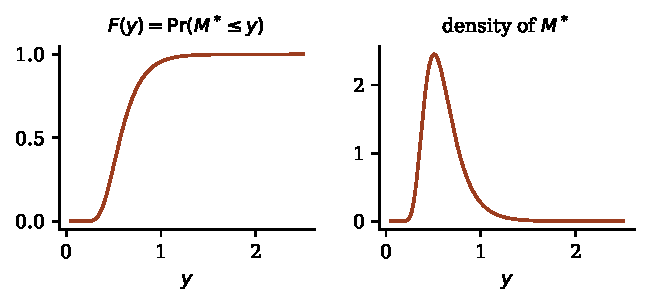
\includegraphics[width=\textwidth]{figs/mstar.pdf}
\caption{The distribution function $F(y)=\prod_n(1-e^{-2\pi ny})^{24}$ of $M^*=\max_{j\le24,\,n\ge1}E_{j,n}/(2\pi n)$, with $E_{j,n}$ independent standard exponential variables (left), and its density (right). The function $e^{-2\pi y}F(y)$ is $\Delta(iy)$.}
\label{fig:mstar}
\end{figure}

For complex $s$ and $c>0$ let $Q(s,c)=\Gamma(s,c)/\Gamma(s)$ be the regularised upper incomplete gamma function,\index{incomplete gamma function}
\[
Q(s,c)=\frac1{\Gamma(s)}\int_c^\infty t^{s-1}e^{-t}\,dt .
\]
For fixed $c>0$, $\Gamma(\cdot,c)$ and $1/\Gamma$ are entire, so $Q(\cdot,c)$ is entire and vanishes at $s=0,-1,-2,\ldots$. For real $s>0$, $Q(s,c)=\Prob(G_s\ge c)$, where $G_s$ has the gamma law of shape $s$ and unit rate.

\begin{theorem}[this book]\label{thm:ch11main}
For every complex $s$,
\[
L(s,\Delta)=\E\bigl[Q(s,2\pi M^*)\bigr].
\]
For real $s>0$, equivalently, $L(s,\Delta)=\Prob(G_s\ge2\pi M^*)$ with $G_s$ independent of $M^*$.
\end{theorem}

\begin{proof}
Recall from Chapter~\ref{ch:02} that for $\operatorname{Re}s>7$ the Dirichlet series converges absolutely and, by termwise integration,
\[
\Lambda(s,\Delta)=(2\pi)^{-s}\Gamma(s)L(s,\Delta)=\int_0^\infty\Delta(iy)y^{s-1}dy.
\]

\emph{Step 1.} By~\eqref{eq:ch11DeltaF}, $0<\Delta(iy)\le e^{-2\pi y}$, and modularity gives $\Delta(iy)=y^{-12}\Delta(i/y)$, which is at most $y^{-12}e^{-2\pi/y}$. Hence $\int_0^\infty\Delta(iy)y^{\sigma-1}dy<\infty$ for every real $\sigma$, locally uniformly in $\sigma$, so the Mellin integral defines an entire function that continues $\Lambda(s,\Delta)$, and $L(s,\Delta)=(2\pi)^s\Lambda(s,\Delta)/\Gamma(s)$ is entire, as Hecke showed \cite{hecke1936}.

\emph{Step 2.} Fix $s$ with $\sigma=\operatorname{Re}s$. For $m>0$,
\[
Q(s,2\pi m)=\frac1{\Gamma(s)}\int_0^\infty t^{s-1}e^{-t}\,1\{t>2\pi m\}\,dt.
\]
Take expectations and exchange the order. Fubini's theorem applies, because by Tonelli's theorem the absolute double integral is $\int_0^\infty t^{\sigma-1}e^{-t}F(t/2\pi)\,dt=(2\pi)^\sigma\int_0^\infty y^{\sigma-1}\Delta(iy)\,dy$, finite by Step 1; in particular $\E|Q(s,2\pi M^*)|<\infty$. As $M^*$ has no atoms, $t=2\pi y$ and~\eqref{eq:ch11DeltaF} give
\[
\E[Q(s,2\pi M^*)]=\frac{(2\pi)^s}{\Gamma(s)}\int_0^\infty y^{s-1}\Delta(iy)\,dy=\frac{(2\pi)^s\Lambda(s,\Delta)}{\Gamma(s)}=L(s,\Delta).
\] At the poles of $\Gamma$ both sides vanish. For real $s>0$, condition on $M^*$.
\end{proof}

\begin{corollary}\label{cor:ch11bounds}
For real $s>0$, $0<L(s,\Delta)<1$.
\end{corollary}

\begin{proof}
$G_s$ and $2\pi M^*$ are independent with positive densities on $(0,\infty)$, so the event $\{G_s\ge2\pi M^*\}$ and its complement both have positive probability.
\end{proof}

The lower bound is positivity of the Mellin integral of $\Delta(iy)$. The next statement is where the probabilistic form helps: a coupling of gamma variables proves it.

\begin{corollary}[this book]\label{cor:ch11monotone}
On $s>0$, $L(s,\Delta)$ is strictly increasing, and $L(s,\Delta)\uparrow1$ as $s\to\infty$.
\end{corollary}

\begin{proof}
For $0<s<t$ realise $G_t=G_s+G'$ with $G'$ of shape $t-s$, independent of $(G_s,M^*)$. Then $\{G_s\ge2\pi M^*\}\subset\{G_t\ge2\pi M^*\}$, and the difference $\{G_s<2\pi M^*\le G_s+G'\}$ has positive probability. Since $G_s\to\infty$ in probability and $M^*<\infty$ almost surely, $\Prob(G_s\ge2\pi M^*)\to1$.
\end{proof}

Numerically, $L(1,\Delta)=0.03744$, $L(3,\Delta)=0.31524$, $L(6,\Delta)=0.79212$, $L(10,\Delta)=0.97981$, $L(12,\Delta)=0.99454$; these values from PARI/GP \cite{pari2023} agree with quadrature of $\E[Q(s,2\pi M^*)]$ to sixteen digits, also at complex points such as $s=6+5i$. Figure~\ref{fig:ch11lvalues} shows the curves for four eta products.

\begin{figure}[t]
\centering
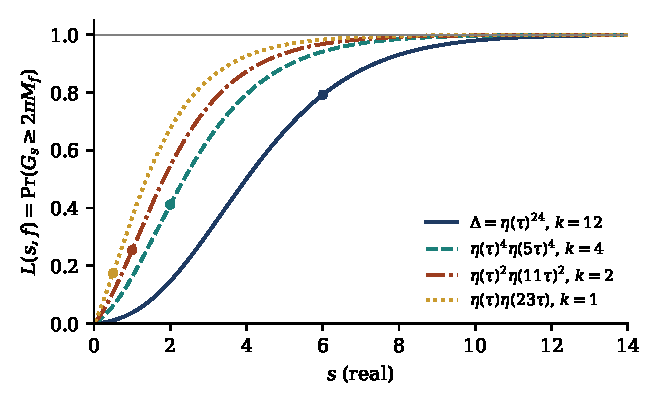
\includegraphics[width=\textwidth]{figs/ch11_lvalues.pdf}
\caption{$L(s,f)=\Prob(G_s\ge2\pi M_f)$ for real $s$, for the multiplicative eta products $\eta(\tau)^{24}$, $\eta(\tau)^4\eta(5\tau)^4$, $\eta(\tau)^2\eta(11\tau)^2$ and $\eta(\tau)\eta(23\tau)$, of weights $k=12,4,2,1$; $G_s$ is a gamma variable of shape $s$, independent of the extreme value $M_f$ of Theorem~\ref{thm:ch11general}. Each curve increases from $0$ to $1$; dots mark the central values $L(k/2,f)$.}
\label{fig:ch11lvalues}
\end{figure}

\section{Modularity as self similarity of the law}

At $\tau=iy$ the transformation $\Delta(-1/\tau)=\tau^{12}\Delta(\tau)$ reads $\Delta(i/y)=y^{12}\Delta(iy)$. In terms of $F$ it is a statement about the law of $M^*$.

\begin{proposition}[this book]\label{prop:ch11selfsim}
For all $y>0$,
\[
F(y)=y^{-12}\,e^{2\pi(y-1/y)}\,F(1/y).
\]
Consequently $F(y)\sim y^{-12}e^{-2\pi/y}$ as $y\to0$, and $1-F(y)\sim24e^{-2\pi y}$ as $y\to\infty$.
\end{proposition}

\begin{proof}
Inserting~\eqref{eq:ch11DeltaF} into $\Delta(i/y)=y^{12}\Delta(iy)$ gives
\[
e^{-2\pi/y}F(1/y)=y^{12}e^{-2\pi y}F(y),
\]
which rearranges to the identity (equivalently, raise~\eqref{eq:ch11Pmod} to the power $24$). The left tail follows from $F(1/y)\to1$, the right tail from $1-P^{24}\sim24(1-P)$.
\end{proof}

We checked the identity at $y=0.5,0.8,1.3$ to fifteen digits. So the law of $M^*$ on $(0,1)$ is determined by its law on $(1,\infty)$, and modularity exchanges the two tails: $\Prob(1/M^*\ge x)\sim x^{12}e^{-2\pi x}$ is a gamma tail of shape $13$, while $1-F(y)\sim24e^{-2\pi y}$ is the exponential tail of the $24$ slowest clocks, those with $n=1$.

The functional equation $\Lambda(s,\Delta)=\Lambda(12-s,\Delta)$ is an integrated form of this self similarity. A sharper reading recovers the P\'olya kernel $\Phi_\Delta$ of Chapter~\ref{ch:10} as a conditional law. Put $V_s=G_s/2\pi$.\index{P\'olya kernel}

\begin{proposition}[this book]\label{prop:ch11posterior}
Let $W=\log(G_6/2\pi)$ with $G_6$ independent of $M^*$. Conditionally on $\{G_6\ge2\pi M^*\}$, $W$ has density $\Phi_\Delta$, and for every complex $z$
\[
\Lambda(6+z,\Delta)/\Lambda(6,\Delta)=\E\bigl[e^{zW}\bigm| G_6\ge2\pi M^*\bigr].
\]
\end{proposition}

\begin{proof}
Let $g_6(y)=(2\pi)^6y^5e^{-2\pi y}/120$ be the density of $V_6$. For bounded measurable $h$,
\[
\E\bigl[h(V_6)1\{M^*\le V_6\}\bigr]=\int_0^\infty hFg_6\,dy=\frac{(2\pi)^6}{120}\int_0^\infty h(y)y^5\Delta(iy)\,dy .
\]
Extend to $h(y)=y^z$ by dominated convergence, using the bounds in Step 1 of the proof of Theorem~\ref{thm:ch11main}, and divide by the case $z=0$.
\end{proof}

In Bayesian terms $\Phi_\Delta$ is a posterior: a log gamma prior of shape $6$ on $W$, likelihood $F(e^W)$, and by self similarity a posterior symmetric about $0$, with variance $0.1123518$ as in Chapter~\ref{ch:10}.

\section{Multiplicative eta products}

Let $r_m\ge0$ be integers with $\sum_mm\,r_m=24$, and put
\[
f(\tau)=\prod_m\eta(m\tau)^{r_m}=q\prod_m\prod_{n\ge1}(1-q^{mn})^{r_m}=\sum_{n\ge1}a_nq^n,
\]
of weight $k=\frac12\sum_mr_m$. Dummit, Kisilevsky and McKay \cite{dkm1985}\index{eta product} determined which have multiplicative coefficients; our search over all $1575$ partitions of $24$ (testing $a_{mn}=a_ma_n$ for coprime $m,n$ with $mn\le300$) finds the same thirty: twenty eight of integral weight $1$ to $12$, and $\eta(8\tau)^3$, $\eta(24\tau)$ of weights $\frac32$, $\frac12$. Each is a holomorphic modular form for a congruence subgroup \cite{koehler2011}. The theorem below needs only that $L(s,f)=\sum a_nn^{-s}$ converges absolutely in a right half plane, and its proof checks this directly for every eta product. Let
\[
M_f=\max_m\max_{j\le r_m}\max_{n\ge1}\frac{E_{m,j,n}}{2\pi mn},\qquad F_f(y)=\Prob(M_f\le y)=\prod_mP(my)^{r_m},
\]
the maximum of $r_m$ independent copies of $M/m$ for each $m$.

\begin{theorem}[this book]\label{thm:ch11general}
Let $f=\prod_m\eta(m\tau)^{r_m}$ with $r_m\ge0$ and $\sum_mm\,r_m=24$. Then $f(iy)=e^{-2\pi y}F_f(y)$ for $y>0$, $L(s,f)$ continues to an entire function, and for every complex $s$
\[
L(s,f)=\E\bigl[Q(s,2\pi M_f)\bigr].
\]
For real $s>0$, $L(s,f)=\Prob(G_s\ge2\pi M_f)$; in particular $0<L(s,f)<1$, and $L(s,f)$ increases strictly to $1$ as $s\to\infty$.
\end{theorem}

\begin{proof}
Since $\eta(imy)=e^{-\pi my/12}P(my)$ and $\sum_mmr_m=24$, we get $f(iy)=e^{-2\pi y}F_f(y)$. Next, $(\operatorname{Im}\tau)^6|\Delta(\tau)|$ is invariant under $\SL_2(\Z)$ and tends to $0$ at the cusp, so it is bounded, and $|\eta(\tau)|\le C(\operatorname{Im}\tau)^{-1/4}$. Hence $|f(x+iy)|\le C_fy^{-k/2}$, and $a_n=e^{2\pi ny}\int_0^1f(x+iy)e^{-2\pi inx}\,dx$ at $y=1/n$ gives $|a_n|\le e^{2\pi}C_fn^{k/2}$. So $L(s,f)$ converges absolutely for $\operatorname{Re}s>k/2+1$, where termwise integration gives $(2\pi)^{-s}\Gamma(s)L(s,f)=\int_0^\infty f(iy)y^{s-1}\,dy$. By~\eqref{eq:ch11Pmod}, $P(x)\le e^{\pi/12}x^{-1/2}e^{-\pi/(12x)}$ for $x\le1$, so $F_f(y)\le Cy^{-k}e^{-c/y}$ for small $y$, with $c=\frac{\pi}{12}\sum_mr_m/m>0$. These two facts replace the appeal to Chapter~\ref{ch:02} and Step~1 in the proof of Theorem~\ref{thm:ch11main}. Since $F_f$ has a positive derivative on $(0,\infty)$, the rest of that proof and the proofs of Corollaries~\ref{cor:ch11bounds} and~\ref{cor:ch11monotone} apply word for word.
\end{proof}

Multiplicativity is not used in the proof. It is what gives the left side an Euler product, and so what makes the right side arithmetic.

\subsection{An elliptic curve}

The product $\eta(\tau)^2\eta(11\tau)^2$ is the newform of weight $2$ and level $11$ attached by Eichler and Shimura \cite{eichler1954,shimura1971} to the elliptic curve $E=11a$, $y^2+y=x^3-x^2-10x-20$. Here $M_f$ is the maximum of two copies of $M$ and two copies of $M/11$, and since $Q(1,c)=e^{-c}$ the theorem at $s=1$ reads
\[
L(E,1)=\E\bigl[e^{-2\pi M_f}\bigr]=\Prob(E_0\ge2\pi M_f)=0.2538419\ldots,
\]
with $E_0$ a standard exponential independent of $M_f$. The value agrees with PARI/GP to sixteen digits, and $L(E,1)/\Omega_E=0.2000000$ with $\Omega_E=1.2692093$, the value $c_{11}/|E(\Q)_{\mathrm{tors}}|^2=5/25$ (Tamagawa number $5$ at $11$, torsion of order $5$) predicted by the Birch and Swinnerton Dyer formula \cite{bsd1965} with trivial Tate Shafarevich group.\index{Birch and Swinnerton Dyer conjecture}

The probability is positive, so the analytic rank is $0$, and hence the Mordell Weil rank is $0$ by Kolyvagin \cite{kolyvagin1988} with Gross and Zagier \cite{grosszagier1986}. But positivity is equally visible from the Mellin integral of $f(iy)>0$, so this adds interpretation, not information; the same holds for all eight weight two multiplicative eta products, of levels $11,14,15,20,24,27,32,36$.

\subsection{Higher weight, weight one and theta series}

For $\eta(\tau)^4\eta(5\tau)^4$, of weight $4$ and level $5$, $L(2,f)=0.4118613$ is the probability that $G_2\ge2\pi M_f$; Table~\ref{tab:ch11values} gives more.

The weight one product $\eta(\tau)\eta(23\tau)$ is classical. It is half the difference of the theta series of $x^2+xy+6y^2$ and $2x^2+xy+3y^2$, and its coefficient at a prime $p\ne23$ is $N_p-1$, with $N_p$ the number of roots of $x^3-x-1$ modulo $p$ (checked for $p<400$; Chapter~\ref{ch:lap} compares all prime powers below $2\cdot10^5$). By Hecke \cite{hecke1937} its $L$ function is the Artin $L$ function\index{Artin $L$ function} $L(s,\rho)=\zeta_{\Q(\theta)}(s)/\zeta(s)$ of the two dimensional representation of $S_3$ of Chapter~\ref{ch:03}, with $\theta=1.3247\ldots$ the real root of $x^3-x-1$. Theorem~\ref{thm:ch11general} says that this Artin $L$ function is an expectation,
\[
L(s,\rho)=\E\bigl[Q\bigl(s,2\pi\max(M,M'/23)\bigr)\bigr],
\]
with $M,M'$ independent copies of $M$. At $s=1$ the class number formula for $\Q(\theta)$ (signature $(1,1)$, class number $1$, regulator $\log\theta$) gives
\[
\Prob\bigl(E_0\ge2\pi\max(M,M'/23)\bigr)=\frac{2\pi\log\theta}{\sqrt{23}}=0.3684093\ldots,
\]
which we checked to sixteen digits. At the centre, $L(\frac12,\rho)=0.1740363$.

The two forms of half integral weight are theta series of Dirichlet characters,
\[
\eta(24\tau)=\sum_{n\ge1}\chi_{12}(n)q^{n^2},\qquad\eta(8\tau)^3=\sum_{n\ge1}\chi_{-4}(n)\,n\,q^{n^2},
\]
with Dirichlet series $L(2s,\chi_{12})$ and $L(2s-1,\chi_{-4})$; Chapter~\ref{ch:beta} builds the P\'olya kernels of $L(s,\chi_{12})$ and $L(s,\chi_{-4})$ from them. For independent copies $M_1,M_2,M_3$ of $M$,
\[
\frac\pi4=\Prob\Bigl(E_0\ge\frac\pi4\max_{j\le3}M_j\Bigr),\qquad \beta(2)=\Prob\Bigl(G_{3/2}\ge\frac\pi4\max_{j\le3}M_j\Bigr),
\]
where $\beta(2)=L(2,\chi_{-4})=0.9159656$ is Catalan's constant, and $L(1,\chi_{12})=\log(2+\sqrt3)/\sqrt3=\Prob(G_{1/2}\ge\pi M/12)=0.7603460$. All three were checked by quadrature to twelve digits.

\begin{table}[t]
\centering
\small
\begin{tabular}{@{}lrrlll@{}}
\toprule
$f$ & $N$ & $k$ & $L(\frac k2,f)$ & $L(\frac{k+1}2,f)$ & $L(k,f)$\\
\midrule
$\eta(\tau)^{24}$ & 1 & 12 & 0.7921228 & 0.8393455 & 0.9945437\\
$\eta(\tau)^8\eta(2\tau)^8$ & 2 & 8 & 0.6812925 & 0.7543068 & 0.9710803\\
$\eta(\tau)^6\eta(3\tau)^6$ & 3 & 6 & 0.5600387 & 0.6552302 & 0.9190337\\
$\eta(2\tau)^{12}$ & 4 & 6 & 0.7805377 & 0.8543050 & 0.9862573\\
$\eta(\tau)^4\eta(5\tau)^4$ & 5 & 4 & 0.4118613 & 0.5320174 & 0.7938049\\
$\eta(3\tau)^8$ & 9 & 4 & 0.7599657 & 0.8578161 & 0.9757577\\
$\eta(\tau)^3\eta(7\tau)^3$ & 7 & 3 & 0.3329818 & 0.4672118 & 0.6875637\\
$\eta(\tau)^2\eta(11\tau)^2$ & 11 & 2 & 0.2538419 & 0.4070039 & 0.5460480\\
$\eta(\tau)\eta(2\tau)\eta(7\tau)\eta(14\tau)$ & 14 & 2 & 0.3302237 & 0.5008415 & 0.6414713\\
$\eta(\tau)\eta(3\tau)\eta(5\tau)\eta(15\tau)$ & 15 & 2 & 0.3501508 & 0.5228611 & 0.6614752\\
$\eta(6\tau)^4$ & 36 & 2 & 0.7010911 & 0.8618161 & 0.9400130\\
$\eta(\tau)\eta(23\tau)$ & 23 & 1 & 0.1740363 & 0.3684093 & 0.3684093\\
$\eta(2\tau)\eta(22\tau)$ & 44 & 1 & 0.3157625 & 0.5772184 & 0.5772184\\
$\eta(12\tau)^2$ & 144 & 1 & 0.6120576 & 0.8706850 & 0.8706850\\
\bottomrule
\end{tabular}
\caption{$L(s,f)=\Prob(G_s\ge2\pi M_f)$ at $s=\frac k2,\frac{k+1}2,k$ for fourteen multiplicative eta products $f$ of level $N$ and weight $k$ (for $k=1$ the last two columns coincide), computed with PARI/GP (\texttt{lfunetaquo}) and confirmed by quadrature; the functional equation of each form was checked numerically.}
\label{tab:ch11values}
\end{table}

Every entry of Table~\ref{tab:ch11values} lies in $(0,1)$, and each row increases with $s$, as Theorem~\ref{thm:ch11general} requires. Within each weight the values grow with the level: the clocks of $\eta(m\tau)$ ring at rates $2\pi mn$, so large $m$ makes $M_f$ small and easy to beat.

\section{Zeros as a probabilistic statement}

If $\rho$ is a zero of $L(s,\Delta)$, Theorem~\ref{thm:ch11main} gives $\E[Q(\rho,2\pi M^*)]=0$. At the first zero $\rho=6+9.2223794\,i$ our quadrature of the left side has modulus below $10^{-15}$. At the trivial zeros $s=0,-1,-2,\ldots$, $Q(s,c)=0$ for \emph{every} $c>0$, so the integrand itself vanishes. The nontrivial zeros arise by cancellation. For fixed $c>0$, $s\mapsto Q(s,c)$ also has complex zeros. For $c=2\pi y$, with $y$ the $10\%$, $50\%$ and $90\%$ quantiles of $M^*$, the zeros of smallest positive imaginary part are near $5.293+6.081i$, $7.003+7.009i$ and $9.669+8.264i$, off the line $\operatorname{Re}s=6$; the zeros of $L(s,\Delta)$ appear only after averaging. The Riemann hypothesis for $\Delta$ takes the following form, which is a reformulation, not progress.

\begin{conjecture}[Riemann hypothesis for $\Delta$, extreme value form]\label{conj:ch11rh}
If $0<\operatorname{Re}s<12$ and $\E[Q(s,2\pi M^*)]=0$, then $\operatorname{Re}s=6$.
\end{conjecture}

Hecke's formula
\[
\Lambda(s,\Delta)=\sum_{n\ge1}\tau(n)\bigl[\Gamma(s,2\pi n)(2\pi n)^{-s}+\Gamma(12-s,2\pi n)(2\pi n)^{s-12}\bigr],
\]
obtained by splitting the Mellin integral at $y=1$ and applying modularity on $(0,1)$, is also an incomplete gamma expansion, but its terms carry the signs of $\tau(n)$; ours averages one kernel against a probability law. For Riemann's $\xi$ the analogous probabilistic formula is $2\xi(s)=\E[Y^s]$ of Biane, Pitman and Yor \cite{bpy2001}, with $Y$ a constant multiple of the maximum of a Brownian excursion (Chapter~\ref{ch:10}). Proposition~\ref{prop:ch11posterior} gives $\Lambda(s,\Delta)$ a probabilistic reading of the same kind, and on the reciprocal side $\xi(\frac12)/\xi(\frac12+\sqrt s)$ is the Laplace transform of a generalized gamma convolution if and only if the Riemann hypothesis holds (Polson~\cite{polson2017}; Theorem~\ref{thm:10bmain}).

Why does this not prove the Riemann hypothesis? First, positivity of a mixing law controls the transform on the real axis (Corollary~\ref{cor:ch11monotone}), not the cancellation that creates zeros. Second, Theorem~\ref{thm:ch11general} holds for every eta product with $\sum mr_m=24$, multiplicative or not, so it does not see the Euler product, and without an Euler product zeros can leave the line, as Davenport and Heilbronn showed \cite{davenportheilbronn1936}. Third, the known sufficient conditions for a Fourier transform to have only real zeros \cite{polya1926,debruijn1950,newman1976} rest on special structure of the kernel (an explicit form in the theorems of P\'olya and de Bruijn, the Lee Yang property in Newman's), and nothing we have shown about $M^*$ supplies such structure. What the representation does provide is an exact probabilistic formula and an unbiased estimator of $L$ at complex points, though one whose variance grows exponentially with the height, as the next section shows.

\section{Monte Carlo}

Theorem~\ref{thm:ch11main} turns evaluation of $L(s,\Delta)$ into sampling. We truncate the maximum at $n\le N$ and call the result $M^*_N\le M^*$. Since $M^*_N\ne M^*$ requires some clock with $n>N$ to ring after $M^*_N$, the union bound gives
\[
\Prob\bigl(M^*>y\ge M^*_N\bigr)\le24\sum_{n>N}e^{-2\pi ny}=\frac{24\,e^{-2\pi(N+1)y}}{1-e^{-2\pi y}} .
\]
For real $s>0$ the bias is $\Prob(M^*_N\le V_s<M^*)$, at most the integral of the smaller of $1$ and this bound against the density of $V_s$, which for $s=6$ and $N=400$ is $1.2\times10^{-13}$. The algorithm draws $E_{j,n}$ for $j\le24$, $n\le N$, sets $m_r=\max_{j,n}E_{j,n}/(2\pi n)$, and returns the mean and standard error of $Q(s,2\pi m_r)$ over $R$ draws. With $N=400$ and $R=20000$ draws we obtained $0.7929\pm0.0012$ (one standard error) for $L(6,\Delta)=0.7921$. The empirical $10\%$, $50\%$, $90\%$ quantiles of $M^*$ were $0.394$, $0.569$, $0.869$, against exact values $0.3935$, $0.5708$, $0.8650$. For real $s>0$ the estimator is the conditional expectation of $1\{G_s\ge2\pi M^*_N\}$ given $M^*_N$, so by the Rao Blackwell theorem its variance is smaller, in our runs by a factor of about five. For a fixed sample, $s\mapsto R^{-1}\sum_rQ(s,2\pi m_r)$ is an entire empirical $L$ function. On the critical line, however, the summands are large while $L$ is not: for fixed $c$, $|Q(6+it,c)|\sim c^6e^{-c}e^{\pi t/2}/(\sqrt{2\pi}\,t^{13/2})$ as $t\to\infty$, because $1/|\Gamma(6+it)|$ grows like $e^{\pi t/2}$, and the standard deviation of $Q(6+it,2\pi M^*)$, computed by quadrature, is $0.18$ at $t=0$, $22$ at the first zero $t=9.22$ and $4.0\times10^6$ at $t=20$. Locating zeros by simulation therefore requires a cancellation that grows exponentially with the height.

\section{Hitting times}

If coupon $(j,n)$ is collected at time $E_{j,n}/(2\pi n)$, the number of coupons still missing at time $t>0$ is finite, with mean $24\sum_ne^{-2\pi nt}$. So $M^*$ is the time at which a collection that starts with infinitely many missing coupons is completed: the hitting time\index{hitting time} of the empty set by the decreasing Markov process of missing coupons, which enters from an infinite configuration. For real $s>0$, $L(s,\Delta)$ is the probability that the collection is completed before an independent gamma clock of shape $s$ and rate $2\pi$ rings.

The laws that Biane, Pitman and Yor \cite{bpy2001} build from theta functions are laws of Brownian functionals. Is $M$ a Brownian functional? We do not know, but a related identity holds. Let $K=\sup_{t\le1}|b_t|$ for a standard Brownian bridge $b$, so that $\Prob(K\le x)=\sum_{n\in\Z}(-1)^ne^{-2n^2x^2}$ is Kolmogorov's law \cite{kolmogorov1933}.

\begin{proposition}[this book]\label{prop:ch11kolmogorov}
$K^2$ has the law of the maximum of independent exponential variables, one of rate $2j$ for each even $j\ge2$ and two of rate $2j$ for each odd $j\ge1$. With $M_1,M_2,M_3$ independent copies of $M$, and $K$ independent of $M_3$,
\[
\max(M_1,M_2)\overset{d}{=}\max\bigl(K^2/\pi,\,M_3/2\bigr).
\]
\end{proposition}

\begin{proof}
Jacobi's triple product gives
\[
\sum_{n\in\Z}(-1)^nq^{n^2}=\prod_{n\ge1}(1-q^{2n})(1-q^{2n-1})^2.
\]
With $q=e^{-2x^2}$ the left side is $\Prob(K^2\le x^2)$ and each factor $1-q^j$ is the probability that an exponential variable of rate $2j$ is at most $x^2$; independence gives the first claim. The same identity in the form $\sum_n(-1)^nq^{n^2}=\eta(\tau)^2/\eta(2\tau)$, at $q=e^{-2\pi y}$, reads $P(y)^2=\Prob(K^2\le\pi y)\,P(2y)$, which is the second claim.
\end{proof}

We checked it at $y=0.1,0.2,0.5$ to fifteen digits. It suggests, but does not establish, that $M$ can be realised through passage or exit times of a diffusion. The simplest mechanism is excluded: the passage time of a one dimensional diffusion from an entrance or reflecting boundary to a fixed level is a sum of independent exponential variables \cite{kent1980}, and $M$ is not (Exercise~\ref{ex:ch11laplace}).

\begin{problem}\label{prob:ch11brownian}
Find a natural Brownian or Bessel functional with the law of $M$, or of $M^*$, or show that none exists among first passage and last exit times of one dimensional diffusions.
\end{problem}

\section{Notes}

That $\prod_n(1-e^{-2\pi ny})$ is a distribution function is elementary, and such products pervade the probabilistic literature on theta functions, from Kolmogorov \cite{kolmogorov1933} to Biane, Pitman and Yor \cite{bpy2001}. What we have not seen before is the representation of $L$ functions of eta products as expectations of incomplete gamma functions at an extreme value, with its consequences: special values as probabilities, monotonicity, modular self similarity, and the posterior reading of the P\'olya kernel. These are the results we label as ours.

Martin \cite{martin1996} classified the multiplicative eta quotients; for quotients our argument fails, since $1/(1-e^{-2\pi ny})$ is not a probability. K\"ohler \cite{koehler2011} is the reference for eta products and theta series, Gumbel \cite{gumbel1958} for extreme values, and Thorin \cite{thorin1977} and Bondesson \cite{bondesson1992} for gamma convolutions. Hecke's formula underlies the evaluation of $L$ functions in PARI/GP and the LMFDB \cite{lmfdb}.

\section{Exercises}

\begin{enumerate}
\item\label{ex:ch11mean} Prove $\E[M]=2/\sqrt3-3/\pi$. (Integrate the pentagonal series for $1-P(y)$ termwise, pair $k$ with $-k$, and evaluate $\int_0^1x(1-x^2)/(1+x^3)\,dx=2\pi/(3\sqrt3)-1$.)

\item Using $\Prob(aG_s<E)=\E[e^{-aG_s}]=(1+a)^{-s}$ for a standard exponential $E$ independent of $G_s$, and a union bound, prove for real $s>1$ that $1-L(s,f)\le\sum_mr_m\sum_{n\ge1}(1+mn)^{-s}$. Evaluate the bound for $\Delta$ at $s=12$ and compare with $1-L(12,\Delta)=0.0054563$.

\item Show that $M^*$ has density $2\pi(1-E_2(iy))F(y)$. Use the transformation law $E_2(-1/\tau)=\tau^2E_2(\tau)+6\tau/(\pi i)$ and Proposition~\ref{prop:ch11selfsim} to find its behaviour as $y\to0$.

\item Prove $\E[K^2]=\pi^2/12$ from Kolmogorov's series. Deduce from Proposition~\ref{prop:ch11kolmogorov} that $\E[\max(M_1,M_2)]\le\pi/12+\E[M]/2$, and check it numerically.

\item For real $s\in(0,12)$ let $W_s$ be $\log(G_s/2\pi)$ conditioned on $\{G_s\ge2\pi M^*\}$. Show that $\E[e^{zW_s}]=\Lambda(s+z,\Delta)/\Lambda(s,\Delta)$, that the law of $W_s$ is the exponential tilt of the law of $W_6$ by $e^{(s-6)u}$, and that $W_{12-s}\overset{d}{=}-W_s$.

\item\label{ex:ch11laplace} Show that $\E[e^{-uM}]=\sum_{k\in\Z}(-1)^ku/(u+\pi k(3k-1))$ for $\operatorname{Re}u>0$, and, using $\sum_{k\in\Z}(-1)^k/(k-a)=-\pi/\sin\pi a$, that with $w=\sqrt{1-12u/\pi}$
\[
\E\bigl[e^{-uM}\bigr]=\frac uw\Bigl(\csc\frac{\pi(1-w)}6-\csc\frac{\pi(1+w)}6\Bigr).
\]
Deduce that the meromorphic continuation of $\E[e^{-uM}]$ vanishes at $u=-35\pi/12$, and conclude that $M$ is not a sum of independent exponential variables. (The Laplace transform of $\sum_jE_j/\lambda_j$ is the reciprocal of the entire function $\prod_j(1+u/\lambda_j)$.)
\end{enumerate}

\section{Open computational problems}

\begin{compproblem}[Tables of the laws $M_f$]
Objective: reference tables of the laws $M_f$ for all thirty multiplicative eta products. Objects and scale: $F_f(y)=\prod_mP(my)^{r_m}$, densities, quantiles at levels $10^{-6},\ldots,1-10^{-6}$, means, variances and the first twenty negative moments, to $50$ digits. Route: the pentagonal series for $my\ge1$ and~\eqref{eq:ch11Pmod} above, in PARI/GP or mpmath; Newton iteration for quantiles. Deliverable: tables and a common plot of all thirty laws. Why it matters: these laws are the arithmetic content of Theorem~\ref{thm:ch11general}, and their tails encode weight and level through self similarity.
\end{compproblem}

\begin{compproblem}[Variance reduction and zero location]
Objective: make $\E[Q(s,2\pi M_f)]$ a practical estimator of $L(s,f)$ on the critical line. For $\Delta$ at $s=6+it$ the plain estimator has standard deviation $0.18$ at $t=0$, $22$ at the first zero and $4.0\times10^6$ at $t=20$, growing like $e^{\pi t/2}t^{-13/2}$. Objects and scale: $\Delta$ on $s=6+it$ and $\eta(\tau)^2\eta(11\tau)^2$ on $s=1+it$ for $0\le t\le30$, with up to $10^9$ draws. Route: GPU sampling of truncated maxima; control variates from the slowest clocks, which have equal rates (the $24$ clocks of rate $2\pi$ for $\Delta$, the two of rate $2\pi$ for the level $11$ form), so that their maximum has R\'enyi's representation, and from the exact values on the real axis; stratification on quantiles of $M_f$; randomised quasi Monte Carlo through the inverse distribution function. Deliverable: for each method the variance as a function of $t$ and its exponential rate, and the largest height up to which the zeros of the sample average locate the zeros of $L(s,f)$ to within $0.01$, with error bars. Why it matters: an estimator able to locate zeros would give a probabilistic certificate of their positions, independent of the approximate functional equation, and the growth rate measures the cancellation that any probabilistic route to the zeros must overcome.
\end{compproblem}

\begin{compproblem}[Eigenforms that are not eta products]
Objective: extend the representation to Hecke eigenforms $f$ for which $g_f(y)=e^{2\pi y}f(iy)$ is not a distribution function; when the root number is $-1$, $f(iy)$ changes sign. Since $g_f$ is smooth and of bounded variation, with $g_f(0+)=0$ and $g_f(\infty)=1$, its Jordan decomposition gives $g_f=aF_1-bF_2$ with distribution functions $F_1,F_2$ on $(0,\infty)$, $a-b=1$, and $a+b$ equal to the total variation $V_f$ of $g_f$, the least possible value; the proof of Theorem~\ref{thm:ch11general} then gives $L(s,f)=a\E[Q(s,2\pi X_1)]-b\E[Q(s,2\pi X_2)]$ with $X_i$ of law $F_i$. Objects and scale: all newforms of weight $2$ with rational coefficients and level up to $500$, and the level one eigenforms of weights $16$ to $24$. Route: $q$ expansions from PARI/GP \texttt{mfinit} or the LMFDB, with the Fricke involution for small $y$; $V_f$ by quadrature of $|g_f'|$; linear programming over mixtures of the laws $\prod_mP(my)^{r_m}$ and their rescalings, to approximate $F_1$ and $F_2$ by extreme value laws. Deliverable: for each form $V_f$ and $b=(V_f-1)/2$, against level, weight, root number and rank, and the error of the best extreme value approximations. Why it matters: $b$ measures the distance from the positive world of this chapter; it is positive whenever $L(\frac k2,f)=0$, in particular for every elliptic curve of positive rank, since then $L(1,f)=0$ by Kolyvagin's theorem \cite{kolyvagin1988}.
\end{compproblem}


\part{Inference and Open Problems}
\chapter[Haar Measure and the p* Formula]{Right Haar Measure, Transformation Models and the p* Formula}\label{ch:11b}

In 1933 Alfr\'ed Haar proved that every separable locally compact group carries a measure invariant under translation \cite{haar1933}; von Neumann's uniqueness theorems and Weil's book of 1940 completed the theory in the generality used today. Statisticians met the same measure from the other side. Fisher's fiducial argument \cite{fisher1935}, Fraser's structural inference \cite{fraser1968} and the invariant estimation theory of Stein \cite{stein1965} and Hora and Buehler \cite{horabuehler1966} live on groups such as the affine group of the line, which are not unimodular: their left and right Haar measures differ, and the right one is the prior whose posterior reproduces the fiducial distribution and whose invariant credible sets have exact frequentist coverage. Barndorff Nielsen's $p^*$ formula \cite{barndorffnielsen1983} uses the left one: in a transformation model $|\hat\jmath|^{1/2}d\hat g$ is a left Haar measure, which is why $p^*$ is exact there.

This chapter puts the two traditions side by side, because the affine group of the line is, up to isomorphism, the triangular subgroup of $\SL_2(\R)$ that acts simply transitively on the upper half plane. Sato Tate groups are compact, so left and right Haar measures agree and Haar measure is the law of Frobenius (Chapter~\ref{ch:04}); in Chapter~\ref{ch:12} it enters the likelihood. The upper half plane, by contrast, is an orbit of a group that is not unimodular, and its hyperbolic area is the image of left Haar measure. Duke's theorem says that Heegner points equidistribute for this measure, a noncompact analogue of Sato Tate. Haar measures also normalise volumes, Tamagawa numbers and the period formulas behind central $L$ values. The statistical theorems are classical, and we prove Theorems~\ref{thm:11bpstar} and \ref{thm:11bright} in the generality of Definition~\ref{def:11bmodel}; Proposition~\ref{thm:11brefprior} on reference priors for conjugacy classes and the computations are new.

\section{Haar measure on locally compact groups}

Left and right Haar measures can differ. We define the modular function that measures the difference, compute both measures for the affine group and the Borel subgroup of $\GL_2$, and transport them to the upper half plane and the Bruhat Tits tree.

\subsection{Existence, uniqueness and the modular function}

Let $G$ be a locally compact Hausdorff group. A \emph{left Haar measure} is a nonzero Radon measure $\mu_l$ with $\mu_l(gE)=\mu_l(E)$ for all Borel $E$ and $g\in G$; a right Haar measure satisfies $\mu_r(Eg)=\mu_r(E)$.\index{Haar measure}

\begin{theorem}[Haar, von Neumann, Weil]\label{thm:11bhaar}
Every locally compact group has a left Haar measure, unique up to a positive constant.
\end{theorem}

Haar \cite{haar1933} proved existence for second countable groups; von Neumann proved uniqueness for compact groups \cite{vonneumann1934} and then for the groups of Haar's theorem \cite{vonneumann1936}; and Weil \cite{weil1940} proved existence and uniqueness without countability assumptions. A modern proof is in \cite{folland1995}. If $\mu_l$ is a left Haar measure and $g\in G$, then $E\mapsto\mu_l(Eg)$ is again left invariant, so by uniqueness
\begin{equation}\label{eq:11bmodular}
\mu_l(Eg)=\Delta_G(g)\,\mu_l(E)
\end{equation}
for a number $\Delta_G(g)>0$ independent of $E$. This is our convention for the \emph{modular function}; it is that of \cite{folland1995}. The map $\Delta_G:G\to\R_{>0}$ is a continuous homomorphism, and in differential form $d\mu_l(xg)=\Delta_G(g)\,d\mu_l(x)$.\index{modular function}

\begin{lemma}\label{thm:11bleftright}
The measure $d\mu_r(x)=\Delta_G(x)^{-1}d\mu_l(x)$ is a right Haar measure, and every right Haar measure is a multiple of it. For a Lie group $\Delta_G(g)=|\det\operatorname{Ad}(g)|^{-1}$.
\end{lemma}

\begin{proof}
Substituting $x=yg$ and using \eqref{eq:11bmodular},
\[\mu_r(Eg)=\int 1_{Eg}(x)\,\frac{d\mu_l(x)}{\Delta_G(x)}=\int 1_E(y)\,\frac{\Delta_G(g)\,d\mu_l(y)}{\Delta_G(y)\Delta_G(g)}=\mu_r(E).\]
Uniqueness follows from Theorem~\ref{thm:11bhaar} applied to the opposite group. For the Lie group formula, let $\mu_l$ be given by a left invariant volume form $\omega$, determined by its value $\omega_e$ on the Lie algebra. Right translation $R_g:x\mapsto xg$ commutes with left translations, so it pulls $\omega$ back to the left invariant form with value $\omega_e\circ\operatorname{Ad}(g^{-1})=\det\operatorname{Ad}(g)^{-1}\,\omega_e$ at $e$, and $\mu_l(Eg)=\int_E|R_g^*\omega|=|\det\operatorname{Ad}(g)|^{-1}\mu_l(E)$.
\end{proof}

$G$ is \emph{unimodular} if $\Delta_G\equiv1$, in which case left and right Haar measures coincide.\index{unimodular group}

\begin{example}[Unimodular groups]\label{ex:11bunimodular}
(i) Compact groups: $\Delta_G(G)$ is a compact subgroup of $\R_{>0}$, hence $\{1\}$. So a compact group, in particular a Sato Tate group, has exactly one Haar probability measure, and the phrase ``Haar measure'' in Chapters~\ref{ch:04} and \ref{ch:12} is unambiguous. (ii) $\GL_n(F)$ for $F=\R$ or $\Q_p$: on the matrix space $M_n(F)$ with additive Haar measure $dx$, left and right multiplication by $g$ both scale $dx$ by $|\det g|^n$, so $|\det x|^{-n}dx$ is a left and right Haar measure. (iii) $\SL_2(\R)$ and $\SL_2(\Q_p)$ are perfect groups, equal to their commutator subgroups, and $\Delta_G$ is a homomorphism into an abelian group, so it is trivial. (iv) Connected nilpotent Lie groups: every $g$ is $\exp X$ for some $X$ in the Lie algebra, and $\operatorname{Ad}(g)=\exp(\operatorname{ad}X)$ is unipotent, so $\det\operatorname{Ad}(g)=1$.
\end{example}

\subsection{The affine group and the Borel subgroup}

The simplest group that is not unimodular is the affine group of the line,
\[
B=\Bigl\{(a,b)=\begin{pmatrix}a&b\\0&1\end{pmatrix}:a>0,\ b\in\R\Bigr\},\qquad (a,b)(a',b')=(aa',ab'+b),
\]
acting on $\R$ by $x\mapsto ax+b$.\index{affine group}

\begin{proposition}\label{thm:11baffine}
On $B$, $d\mu_l=a^{-2}\,da\,db$ and $d\mu_r=a^{-1}\,da\,db$, and $\Delta_B(a,b)=a^{-1}$.
\end{proposition}

\begin{proof}
Left translation by $(\alpha,\beta)$ is the map $(a,b)\mapsto(\alpha a,\alpha b+\beta)$, whose Jacobian matrix with respect to $(a,b)$ is $\operatorname{diag}(\alpha,\alpha)$, of determinant $\alpha^2$. Hence for the image point $(a',b')$ we have $da'\,db'/a'^2=\alpha^2\,da\,db/(\alpha^2a^2)=da\,db/a^2$, so $a^{-2}da\,db$ is left invariant. Right translation by $(\alpha,\beta)$ is $(a,b)\mapsto(a\alpha,a\beta+b)$, with Jacobian matrix $\bigl(\begin{smallmatrix}\alpha&0\\\beta&1\end{smallmatrix}\bigr)$ of determinant $\alpha$; then $da'\,db'/a'=\alpha\,da\,db/(a\alpha)=da\,db/a$, so $a^{-1}da\,db$ is right invariant. Under the same right translation $da'\,db'/a'^2=\alpha^{-1}da\,db/a^2$, so $\Delta_B(\alpha,\beta)=\alpha^{-1}$ by \eqref{eq:11bmodular}, in agreement with $d\mu_r=\Delta_B^{-1}d\mu_l$.
\end{proof}

For the Borel subgroup $B_2=\{\bigl(\begin{smallmatrix}a&b\\0&d\end{smallmatrix}\bigr)\}$ of $\GL_2(F)$, $F=\R$ or $\Q_p$, the same Jacobian computation gives $d\mu_l=|a|^{-2}|d|^{-1}da\,db\,dd$, $d\mu_r=|a|^{-1}|d|^{-2}da\,db\,dd$ and $\Delta_{B_2}=|d/a|$ (Exercise~\ref{ex:11bborel}). The inverse $|a/d|$ is the character usually written $\delta_B$ in representation theory, and the normalised induction that defines principal series representations twists by $\delta_B^{1/2}$ precisely to compensate for the failure of unimodularity.

\subsection{Iwasawa decomposition}

Let $G=\SL_2(\R)$ with $K=\mathrm{SO}(2)$ and $B=B^+=\{n(x)a(y)\}$, where $n(x)=\bigl(\begin{smallmatrix}1&x\\0&1\end{smallmatrix}\bigr)$ and $a(y)=\operatorname{diag}(y^{1/2},y^{-1/2})$, $y>0$; or let $G=\GL_2(\Q_p)$ with $K=\GL_2(\Z_p)$ and $B$ the upper triangular group. In both cases $G=BK$ (Iwasawa decomposition), and a Haar measure $dg$ on the unimodular group $G$ factors through left Haar measure on $B$:\index{Iwasawa decomposition}
\begin{equation}\label{eq:11biwasawa}
\int_Gf(g)\,dg=\int_B\int_Kf(bk)\,d\mu_l(b)\,dk ,
\end{equation}
with $dk$ the Haar probability measure on $K$ \cite{bump1997,folland1995}. Formula \eqref{eq:11biwasawa} fixes the normalisation of $dg$; in the $p$ adic case, normalising $\mu_l$ so that the compact group $B\cap K$ has measure one gives $K$ measure one. The proof is the uniqueness argument again: $B\times K$ acts transitively on $G$ by $g\mapsto bgk^{-1}$ with compact stabiliser $B\cap K$, so a measure on $G$ invariant under this action is unique up to scale; Haar measure is one such measure because $G$ is unimodular, and the image of $\mu_l\times dk$ under $(b,k)\mapsto bk$ is another. It is the left, not the right, Haar measure of $B$ that appears.

\subsection{The upper half plane}

$\SL_2(\R)$ acts on $\mathbb H=\{x+iy:y>0\}$ by M\"obius transformations, the stabiliser of $i$ is $\mathrm{SO}(2)$, and so $\mathbb H=\SL_2(\R)/\mathrm{SO}(2)$. Since $n(x)a(y)\cdot z=yz+x$, the group $B^+$ is the affine group $(a,b)=(y,x)$ of Proposition~\ref{thm:11baffine}, acting on $\mathbb H$ simply transitively, and the orbit map $\phi(a,b)=(a,b)\cdot i=b+ia$ is a bijection $B^+\to\mathbb H$.

\begin{proposition}\label{thm:11bhyperbolic}
The image under $\phi$ of left Haar measure $a^{-2}da\,db$ is the hyperbolic area $dx\,dy/y^2$; the image of right Haar measure is $dx\,dy/y$. Every $B^+$ invariant Radon measure on $\mathbb H$ is a multiple of $dx\,dy/y^2$, and this measure is invariant under all of $\SL_2(\R)$. The measure $dx\,dy/y$ is not $B^+$ invariant.
\end{proposition}

\begin{proof}
In coordinates $\phi$ is $(a,b)\mapsto(x,y)=(b,a)$, so the images are as stated. Since $\phi(hg)=h\cdot\phi(g)$, a measure $m$ on $\mathbb H$ is $B^+$ invariant exactly when $\phi^{-1}_*m$ is left invariant on $B^+$; by Theorem~\ref{thm:11bhaar} these are the multiples of $a^{-2}da\,db$. For $g=\bigl(\begin{smallmatrix}\alpha&\beta\\\gamma&\delta\end{smallmatrix}\bigr)\in\SL_2(\R)$ the map $z\mapsto gz$ is holomorphic with derivative $(\gamma z+\delta)^{-2}$, so its real Jacobian is $|\gamma z+\delta|^{-4}$, while $\operatorname{Im}(gz)=y|\gamma z+\delta|^{-2}$; the two factors cancel in $dx\,dy/y^2$. Finally, for $c>0$ the measure $dx\,dy/y$ of $cE$ is $c$ times that of $E$.
\end{proof}

Thus hyperbolic area is the image of left Haar measure. The Iwasawa formula explains why it is invariant under the whole group although $B^+$ is not unimodular: on $G/K$ with $G$ unimodular and $K$ compact the invariant measure is the image of $dg$, and by \eqref{eq:11biwasawa} this image is the image of $d\mu_l$ on $B^+$.

\begin{figure}[t]
\centering
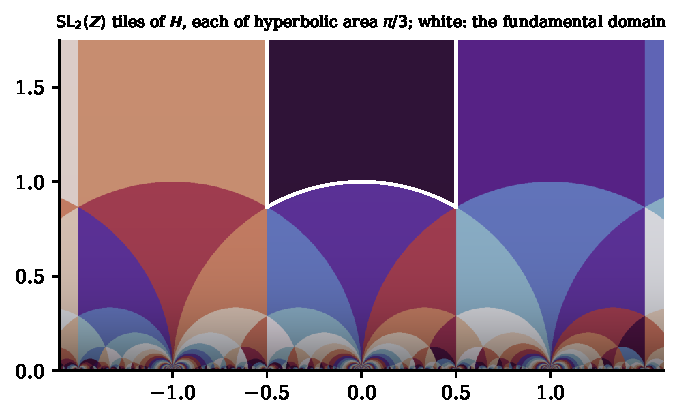
\includegraphics[width=\textwidth]{figs/modular_tessellation.pdf}
\caption{The tiles $\gamma\mathcal F$, $\gamma\in\SL_2(\Z)$, of the upper half plane, coloured by reduction depth; the standard fundamental domain $\mathcal F$ is outlined in white. Each tile has hyperbolic area $\pi/3$ for the left Haar image $dx\,dy/y^2$.}\label{fig:11btess}
\end{figure}

The standard fundamental domain of $\SL_2(\Z)$ is $\mathcal F=\{|x|\le\frac12,\ x^2+y^2\ge1\}$ (Figure~\ref{fig:11btess}), and its area is
\begin{equation}\label{eq:11barea}
\int_{-1/2}^{1/2}\int_{\sqrt{1-x^2}}^\infty\frac{dy}{y^2}\,dx=\int_{-1/2}^{1/2}\frac{dx}{\sqrt{1-x^2}}=2\arcsin\tfrac12=\frac\pi3 .
\end{equation}
Consequently $\frac3\pi\,dx\,dy/y^2$ is the invariant probability measure on $\SL_2(\Z)\backslash\mathbb H$. The Petersson inner product $\langle f,g\rangle=\int_{\mathcal F}f\bar g\,y^k\,dx\,dy/y^2$ of weight $k$ forms integrates against this measure, and Rankin and Selberg's unfolding, the source of $L(s,\Delta\times\Delta)$, uses the same invariance: with $\Gamma_\infty=\{\pm\bigl(\begin{smallmatrix}1&m\\0&1\end{smallmatrix}\bigr):m\in\Z\}$ and $E(z,s)=\sum_{\gamma\in\Gamma_\infty\backslash\SL_2(\Z)}\operatorname{Im}(\gamma z)^s$,
\[
\begin{split}\int_{\mathcal F}|\Delta(z)|^2y^{12}E(z,s)\,\frac{dx\,dy}{y^2}&=\int_0^\infty\!\!\int_0^1|\Delta|^2y^{s+10}\,dx\,dy\\&=\frac{\Gamma(s+11)}{(4\pi)^{s+11}}\sum_{n\ge1}\frac{\tau(n)^2}{n^{s+11}}\end{split}
\]
\cite{iwanieckowalski2004}. The Mellin integral $\Lambda(s,\Delta)=\int_0^\infty\Delta(iy)y^s\,dy/y$ of Chapter~\ref{ch:10} uses a third Haar measure, $dy/y$ on the diagonal torus, which is abelian and therefore unimodular.

\subsection{The Bruhat Tits tree and two Haar shadows}

For a prime $p$ the vertex set of the Bruhat Tits tree $\T_p$ of Chapter~\ref{ch:07} is
\[\GL_2(\Q_p)/\Q_p^\times\GL_2(\Z_p)=\PGL_2(\Q_p)/\PGL_2(\Z_p).\] Normalise Haar measure on the unimodular group $\PGL_2(\Q_p)$ so that the open compact subgroup $\PGL_2(\Z_p)$ has measure one. Each vertex is a coset $g\PGL_2(\Z_p)$, of measure one, so the image of Haar measure on the vertex set is counting measure, the unique invariant measure on a discrete homogeneous space up to scale.\index{Bruhat Tits tree}

Two probability measures on $[-2,2]$ come from Haar measures in this picture. The Plancherel measure of $\PGL_2(\Q_p)$ restricted to the unramified tempered dual, for this normalisation of Haar measure, is the Kesten McKay law $\mu_p$ (Macdonald \cite{macdonald1971}; Chapter~\ref{ch:07}). The Sato Tate law $\ST$ is the image of Haar measure on the compact group $\SU(2)$, the maximal compact subgroup of the dual group $\SL_2(\C)$, under the map to conjugacy classes. One is a shadow of Haar measure on a noncompact $p$ adic group, read through harmonic analysis; the other is a shadow of Haar measure on a compact real form of the complex dual group, read through Weyl's integration formula. They are related by the limit $\mu_p\Rightarrow\ST$ as $p\to\infty$ (Theorem~\ref{thm:07tree}), and arithmetically by Serre's vertical theorem (Theorem~\ref{thm:07serre}) against the horizontal Sato Tate theorem.

\section{Equidistribution on a noncompact quotient}\label{sec:11bduke}

The quotient $\SL_2(\Z)\backslash\mathbb H$ has finite volume but is not compact. Duke's theorem is the equidistribution theorem for its invariant probability measure $\frac3\pi\,dx\,dy/y^2$, the normalised image of left Haar measure.

\subsection{Duke's theorem}

Let $D<-4$ be a fundamental discriminant. A positive definite primitive binary quadratic form $Q=(a,b,c)$ with $b^2-4ac=D$ has a root $z_Q=(-b+i\sqrt{|D|})/(2a)$ in $\mathbb H$, and $Q$ is reduced exactly when $z_Q\in\mathcal F$ (with the usual boundary conventions). The set $\Lambda_D$ of these \emph{Heegner points} (also called CM points) has $h(D)$ elements, the class number of $\Q(\sqrt D)$ (Exercise~\ref{ex:11bclass}).\index{Heegner points}

\begin{theorem}[Duke \cite{duke1988}]\label{thm:11bduke}
As $D\to-\infty$ through fundamental discriminants, $\Lambda_D$ becomes equidistributed in $\SL_2(\Z)\backslash\mathbb H$ for $\frac3\pi\,dx\,dy/y^2$: for every Borel set $\Omega\subset\mathcal F$ whose boundary has measure zero,
\[
\frac{\#(\Lambda_D\cap\Omega)}{h(D)}\longrightarrow\frac3\pi\int_\Omega\frac{dx\,dy}{y^2}.
\]
\end{theorem}

We describe the proof only at the level of its inputs. By the Weyl criterion on the noncompact quotient one must show that the normalised Weyl sums $h(D)^{-1}\sum_{z\in\Lambda_D}\varphi(z)$ tend to $0$ for $\varphi$ a Maass cusp form and for the continuous spectrum. For the Eisenstein series the Weyl sum is an explicit multiple of $\zeta(s)L(s,\chi_D)$, and a subconvex bound for Dirichlet $L$ functions of Burgess type \cite{burgess1963} gives a power saving. For cusp forms Duke related the Weyl sums, through a theta correspondence, to Fourier coefficients of Maass forms of weight one half, and he bounded these coefficients by extending Iwaniec's method for holomorphic forms of half integral weight \cite{iwaniec1987}. Earlier, Linnik had proved the result under a congruence condition on $D$ by an ergodic method \cite{linnik1968}.

The Langlands content is visible through Waldspurger's theorem \cite{waldspurger1981}: the squares of the Fourier coefficients of a half integral weight form are proportional to the central values $L(\frac12,f\otimes\chi_D)$ of the quadratic twists of its Shimura lift $f$, and the toric period formula \cite{waldspurger1985} expresses $|\sum_{\Lambda_D}\varphi|^2$ through central values attached to $\varphi$ and to the quadratic field. In this language equidistribution follows from, and is essentially equivalent to, a subconvex bound for these central values in the $D$ aspect, and Iwaniec's estimate, extended by Duke to Maass forms, is such a bound. We do not attempt the exact constants, which depend on the Haar normalisations discussed in Section~\ref{sec:11btamagawa}.

\subsection{A computation}

For the $60$ fundamental discriminants $D$ in $[-1002999,-1002803]$ we enumerated all reduced primitive forms (computation for this book). There are $28251$ Heegner points, and for each $D$ the count equals the class number $h(D)$ returned by PARI/GP. Above height $t\ge1$ the fundamental domain is the strip $|x|\le\frac12$, so the invariant measure predicts
\[
\Prob(\operatorname{Im}z>t)=\frac3\pi\int_t^\infty\frac{dy}{y^2}=\frac3{\pi t},\qquad t\ge1,
\]
and, given $\operatorname{Im}z>1$, a uniform law for $\operatorname{Re}z$ on $[-\frac12,\frac12]$. Table~\ref{tab:11bduke} and Figure~\ref{fig:11bheegner} compare. The tail agrees with $3/(\pi t)$ to within $3\cdot10^{-3}$ at every height. In units of the binomial standard error $(P(1-P)/28251)^{1/2}$, $P=3/(\pi t)$, which is only a yardstick (the points are not random, and $z_Q$ and $-\bar z_Q$ have the same height), the deviation is $2.4$ at $t=1$ and below one at the other heights. Duke's proof gives a rate $|D|^{-\delta}$, and at $|D|\approx10^6$ this is at least $0.03$ for every $\delta\le\frac14$ (the Lindel\"of value, Computational Problem~\ref{cp:11bduke}), at least ten times the largest deviation. The table is therefore consistent with the theorem but does not test its rate. The horizontal coordinate above height one passes a Kolmogorov Smirnov test for uniformity with $p=0.36$.

\begin{table}[t]
\centering
\small\setlength{\tabcolsep}{4pt}
\begin{tabular}{lcccccc}
\toprule
$t$ & $1$ & $1.5$ & $2$ & $3$ & $5$ & $10$\\
\midrule
data & $0.95193$ & $0.63608$ & $0.47524$ & $0.31769$ & $0.19104$ & $0.09511$\\
$3/(\pi t)$ & $0.95493$ & $0.63662$ & $0.47746$ & $0.31831$ & $0.19099$ & $0.09549$\\
\bottomrule
\end{tabular}
\caption{Heights of the $28251$ Heegner points for the $60$ fundamental discriminants in $[-1002999,-1002803]$ against the invariant tail $3/(\pi t)$; the row ``data'' is the empirical $\Prob(\operatorname{Im}z>t)$.}\label{tab:11bduke}
\end{table}

\begin{figure}[t]
\centering
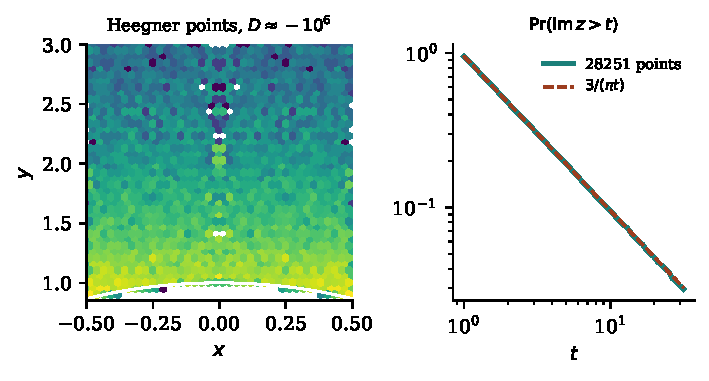
\includegraphics[width=\textwidth]{figs/haar_heegner.pdf}
\caption{Left: density of the $28251$ Heegner points of Table~\ref{tab:11bduke} in the fundamental domain, in hexagonal bins up to height $3$; lighter cells hold more points, and the density decays like $y^{-2}$. Right: the empirical tail $\Prob(\operatorname{Im}z>t)$ against the left Haar prediction $3/(\pi t)$ on logarithmic axes.}\label{fig:11bheegner}
\end{figure}

\begin{remark}[A noncompact Sato Tate theorem]
Sato Tate says that the classes of Frobenius equidistribute for Haar measure on a compact group. Duke's theorem says that the CM points of discriminant $D$ equidistribute for the invariant measure on $\SL_2(\Z)\backslash\SL_2(\R)/\mathrm{SO}(2)$, which on the Iwasawa coordinates is left Haar measure of $B^+$. In both, the limit law is a Haar measure and the proof needs an automorphic input, potential automorphy of symmetric powers \cite{blght2011} in one case and subconvexity for twisted central values in the other. The difference is the cusp: mass could escape to $y=\infty$, and the convergence of $\Prob(\operatorname{Im}z>t)$ to $3/(\pi t)$, which tends to $0$ as $t\to\infty$, says that it does not.
\end{remark}

\section{Transformation models and the p* formula}

In a transformation model the conditional law of the maximum likelihood estimator given an ancillary configuration is explicit, and Barndorff Nielsen's $p^*$ formula reproduces it exactly; outside such models $p^*$ is an approximation of high order.

\subsection{Structural models}

Following Fraser \cite{fraser1968} and Barndorff Nielsen \cite{barndorffnielsen1983,barndorffnielsencox1994}, a \emph{transformation model} is a family of laws generated from one law by a group. We work in the following setting.\index{transformation model}

\begin{definition}\label{def:11bmodel}
Let $G$ be a Lie group of dimension $d$ acting freely on an open set $\mathcal X\subset\R^n$ by affine maps $x\mapsto A_gx+b_g$, and put $\chi(g)=|\det A_g|$, a continuous homomorphism $G\to\R_{>0}$. Let $U$ have a density $f$ on $\mathcal X$, twice continuously differentiable on the open set where it is positive. The \emph{transformation model} is the family of laws of $X=gU$, $g\in G$, with densities
\[
p(x;g)=f(g^{-1}x)\,\chi(g)^{-1}.
\]
We assume that for every $x$ in an open $G$ invariant set $\mathcal X_0\subset\mathcal X$ of full measure the likelihood $g\mapsto p(x;g)$ has a unique maximiser $\hat g(x)$, that $\hat g$ is smooth on $\mathcal X_0$, and that the observed information $j(\hat g;x)=-\nabla^2\ell(\hat g)$, $\ell(g)=\log p(x;g)$, is nonsingular in some (hence every) chart.
\end{definition}

The location scale model $X_i=\mu+\sigma U_i$, $n\ge2$, is the case $G=B$, $g=(\sigma,\mu)$, $\chi(g)=\sigma^n$, with $\mathcal X=\{x\in\R^n:\text{not all }x_i\text{ equal}\}$, on which $B$ acts freely; the scale model $X_i=\theta U_i$ on $(0,\infty)^n$ is the case $G=\R_{>0}$.

\begin{lemma}\label{thm:11bconfig}
(i) $\hat g(hx)=h\hat g(x)$ for $h\in G$. (ii) The \emph{configuration} $a(x)=\hat g(x)^{-1}x$ is a maximal invariant, so its law does not depend on $g$: it is ancillary. (iii) $x=\hat g(x)\,a(x)$, and $A=\{x\in\mathcal X_0:\hat g(x)=e\}$ is a smooth submanifold of dimension $n-d$ such that $\Phi:G\times A\to\mathcal X_0$, $\Phi(h,a)=ha$, is a diffeomorphism.
\end{lemma}

\begin{proof}
(i) $p(hx;g)=f(g^{-1}hx)\chi(g)^{-1}=p(x;h^{-1}g)\chi(h)^{-1}$, so $g$ maximises the left side if and only if $h^{-1}g$ maximises $p(x;\cdot)$, that is $g=h\hat g(x)$. (ii) $a(hx)=\hat g(x)^{-1}h^{-1}hx=a(x)$; and if $a(x)=a(y)$ then $y=\hat g(y)\hat g(x)^{-1}x$ lies on the orbit of $x$. Since $X=gU$, $a(X)=a(U)$ has the law of $a(U)$ for every $g$. (iii) By (i) the derivative of $\hat g$ along the orbit through $x$ is onto, so $\hat g$ is a submersion and $A=\hat g^{-1}(e)$ is a submanifold; $\Phi$ is smooth with smooth inverse $x\mapsto(\hat g(x),\hat g(x)^{-1}x)$.
\end{proof}

\begin{lemma}\label{thm:11bdisint}
Under $\Phi$, Lebesgue measure on $\mathcal X_0$ becomes $\chi(h)\,d\mu_l(h)\,\kappa(da)$ for a measure $\kappa$ on $A$ with a smooth positive density.
\end{lemma}

\begin{proof}
The pull back $\nu(F)=\lambda(\Phi(F))$ of Lebesgue measure $\lambda$ under the diffeomorphism $\Phi$ has a smooth positive density, $\nu=q(h,a)\,d\mu_l(h)\,da$ with $da$ a smooth volume on $A$. Since $\Phi(g'h,a)=g'\Phi(h,a)$ and $\lambda(g'E)=\chi(g')\lambda(E)$, the measure $\nu$ satisfies $\nu(L_{g'}F)=\chi(g')\nu(F)$ for $L_{g'}(h,a)=(g'h,a)$. As $\mu_l$ is left invariant this says $q(g'h,a)=\chi(g')q(h,a)$, hence $q(h,a)=\chi(h)q(e,a)$. Put $\kappa(da)=q(e,a)\,da$.
\end{proof}

\subsection{Exactness of p*}

Barndorff Nielsen's formula approximates the conditional density of the maximum likelihood estimator given an ancillary $a$ by\index{p* formula}
\begin{equation}\label{eq:11bpstar}
p^*(\hat g;g\mid a)=c(a)\,|j(\hat g;x)|^{1/2}\exp\{\ell(g)-\ell(\hat g)\},
\end{equation}
where $x$ is reconstructed from $(\hat g,a)$, $\ell$ is the log likelihood, the density is taken with respect to Lebesgue measure in a chart of $G$, and $c(a)$ makes it integrate to one.

\begin{theorem}[Barndorff Nielsen \cite{barndorffnielsen1980,barndorffnielsen1983}]\label{thm:11bpstar}
In the transformation model of Definition~\ref{def:11bmodel}, conditionally on the maximal invariant $a(X)=a$, the estimator $\hat g$ has density
\begin{equation}\label{eq:11bexact}
p(\hat g;g\mid a)=\frac{f(g^{-1}\hat g\,a)\,\chi(g^{-1}\hat g)}{c_0(a)}\qquad\text{with respect to }d\mu_l(\hat g),
\end{equation}
$c_0(a)=\int_Gf(ka)\chi(k)\,d\mu_l(k)$. Moreover $|j(\hat g;x)|^{1/2}d\hat g=|j(e;a)|^{1/2}\,d\mu_l(\hat g)$ in any chart, with $\mu_l$ normalised to agree with chart Lebesgue measure at $e$, and \eqref{eq:11bpstar} is exactly \eqref{eq:11bexact}.
\end{theorem}

For the location scale group the exact conditional density is due to Fisher \cite{fisher1934}; the identification with $p^*$, and the point that $|\hat\jmath|^{1/2}d\hat g$ is left invariant, are Barndorff Nielsen's. The proof below is written for the generality of Definition~\ref{def:11bmodel}.

\begin{proof}
By Lemma~\ref{thm:11bdisint} the joint density of $(\hat g,a)=\Phi^{-1}(X)$ with respect to $d\mu_l(h)\,\kappa(da)$ is $p(ha;g)\chi(h)=f(g^{-1}ha)\chi(g^{-1}h)$. Dividing by its integral over $h$ gives \eqref{eq:11bexact}, and $c_0(a)<\infty$ for $\kappa$ almost every $a$ by Fubini, since the joint density integrates to one.

For the information, fix $x=\hat g a$ and write $\ell_x(g)=\log p(x;g)$. From $p(\hat ga;g)=f(g^{-1}\hat ga)\chi(g)^{-1}$ we get $\ell_x(g)=\ell_a(\hat g^{-1}g)-\log\chi(\hat g)$. In a chart let $\psi$ denote $g\mapsto\hat g^{-1}g$. Since $e$ maximises $\ell_a$ (because $\hat g(a)=e$), its gradient vanishes there, so the chain rule gives no first order term and
\[
j(\hat g;x)=D\psi(\hat g)^{\top}\,j(e;a)\,D\psi(\hat g),\qquad |j(\hat g;x)|^{1/2}=|\det D\psi(\hat g)|\,|j(e;a)|^{1/2}.
\]
A left invariant measure has chart density $m(g)=m(e)|\det D(L_{g^{-1}})(g)|$, which is $|\det D\psi(\hat g)|$ at $g=\hat g$ when $m(e)=1$. This proves the second claim. Finally
\[
\exp\{\ell_x(g)-\ell_x(\hat g)\}=\frac{f(g^{-1}\hat ga)\chi(g)^{-1}}{f(a)\chi(\hat g)^{-1}}=\frac{f(g^{-1}\hat ga)\chi(g^{-1}\hat g)}{f(a)},
\]
so $p^*\,d\hat g=c(a)|j(e;a)|^{1/2}f(a)^{-1}f(g^{-1}\hat ga)\chi(g^{-1}\hat g)\,d\mu_l(\hat g)$, which is \eqref{eq:11bexact} for $c(a)=f(a)/(c_0(a)|j(e;a)|^{1/2})$.
\end{proof}

\begin{example}[Location and scale]\label{ex:11blocscale}
For $X_i=\mu+\sigma U_i$ with $\hat g=(\hat\sigma,\hat\mu)$, the configuration is $a=(a_i)$ with $a_i=(x_i-\hat\mu)/\hat\sigma$, $\chi(g)=\sigma^n$, and by Proposition~\ref{thm:11baffine} $d\mu_l=d\hat\mu\,d\hat\sigma/\hat\sigma^2$. With $f$ now the density of each $U_i$, Theorem~\ref{thm:11bpstar} gives the conditional density of $(\hat\mu,\hat\sigma)$ given $a$ as proportional to $\hat\sigma^{n-2}\sigma^{-n}\prod_if((\hat\mu-\mu+\hat\sigma a_i)/\sigma)$, Fisher's formula. Directly, $j(\hat g;x)=\hat\sigma^{-2}H(a)$ with $H(a)$ a function of the configuration alone, so $|\hat\jmath|^{1/2}=\hat\sigma^{-2}|H(a)|^{1/2}$ is the left Haar density.
\end{example}

\begin{example}[Exponential scale family]\label{ex:11bexp}
Let $X_1,\dots,X_n$ be independent with density $\theta^{-1}e^{-x/\theta}$ on $(0,\infty)$. Then $\ell(\theta)=-n\log\theta-n\bar x/\theta$, $\hat\theta=\bar x$, $\ell(\hat\theta)=-n\log\hat\theta-n$, and $\ell''(\theta)=n\theta^{-2}-2n\bar x\theta^{-3}$, so $j(\hat\theta)=n/\hat\theta^2$. Hence
\[
p^*(\hat\theta;\theta)=c\,\frac{n^{1/2}}{\hat\theta}\,\frac{\hat\theta^n e^n}{\theta^n}\,e^{-n\hat\theta/\theta}=c\,n^{1/2}e^n\,\frac{\hat\theta^{n-1}}{\theta^n}\,e^{-n\hat\theta/\theta}.
\]
The exact law of $\bar X$ is Gamma with shape $n$ and rate $n/\theta$, with density
\[p(\hat\theta;\theta)=\frac{(n/\theta)^n\hat\theta^{n-1}e^{-n\hat\theta/\theta}}{\Gamma(n)},\]
the same function of $\hat\theta$, so after normalisation, $c=n^{n-1/2}e^{-n}/\Gamma(n)$, $p^*$ is exact. (The configuration $x/\bar x$ is independent of $\bar x$ here, so conditioning is vacuous.) With the unnormalised constant $c=(2\pi)^{-1/2}$ the ratio $p^*/p$ is $\Gamma(n)e^n/(\sqrt{2\pi}\,n^{n-1/2})=1+\frac1{12n}+O(n^{-2})$ by Stirling's formula; numerically $1.0168$, $1.0084$, $1.0042$ for $n=5,10,20$.
\end{example}

\subsection{Beyond group models}

Outside transformation models $p^*$ is an approximation. For a full exponential family and $n$ independent observations, $\hat\theta$ is sufficient, no ancillary is needed, and $p^*$ coincides with the saddlepoint approximation of Daniels \cite{daniels1954} to the density of the sufficient statistic, transformed to $\hat\theta$. With $c=(2\pi)^{-d/2}$ its relative error is $O(n^{-1})$. After renormalisation the relative error is $O(n^{-3/2})$ on normal deviation regions, where $\hat\theta-\theta=O(n^{-1/2})$, and remains $O(n^{-1})$ for larger deviations \cite{barndorffnielsen1983,barndorffnielsencox1994,reid1988}. In curved exponential families the order $O(n^{-3/2})$ holds conditionally on an ancillary that is exact or approximately ancillary to sufficiently high order \cite{barndorffnielsen1980,barndorffnielsencox1994}. Laplace's method explains the shape: expanding $\ell(\theta)-\ell(\hat\theta)$ to second order around $\hat\theta$ makes \eqref{eq:11bpstar} with $c=(2\pi)^{-d/2}$ approximately a normal density for $\hat\theta$ with mean $\theta$ and covariance $\hat\jmath^{-1}$, and $(2\pi)^{-d/2}|\hat\jmath|^{1/2}$ is its normalising constant. Example~\ref{ex:11bexp} shows two of these levels: the constant $(2\pi)^{-1/2}$ is off by Stirling's factor $1+\frac1{12n}+O(n^{-2})$, while the renormalised formula is exact because the model is a group model.

\section{Right Haar priors}\label{sec:11bright}

We prove that the right Haar prior gives invariant credible sets exact frequentist coverage, compute the shortfall of the left Haar prior for normal errors, and check both by simulation.

\subsection{Structural, fiducial and Bayes}

The posterior of the right Haar prior coincides with Fraser's structural distribution and with Fisher's fiducial distribution, and its invariant credible sets are exact confidence sets for every sample size \cite{fraser1968,stein1965,horabuehler1966}; see also \cite{berger1985,eaton1989}. We give a complete proof in the setting of Definition~\ref{def:11bmodel}.\index{right Haar prior}

\begin{theorem}[Fraser; Stein; Hora and Buehler]\label{thm:11bright}
Let the prior be $d\mu_r(g)$, and let $x\in\mathcal X_0$ have configuration $a$ with $c_0(a)<\infty$, which holds for almost every $x$. Under the posterior, the pivot $k=g^{-1}\hat g(x)$ has law
\[
Q_a(dk)=c_0(a)^{-1}f(ka)\chi(k)\,d\mu_l(k),
\]
and under the sampling law $P_g$, conditionally on $a(X)=a$, the pivot $g^{-1}\hat g(X)$ has the same law $Q_a$. Consequently, if $S_a\subset G$ satisfies $Q_a(S_a)=1-\alpha$ for each $a$, the set $C(x)=\{g:g^{-1}\hat g(x)\in S_{a(x)}\}$ has posterior probability $1-\alpha$ and $P_g(g\in C(X))=1-\alpha$ for every $g\in G$ and every $n$.
\end{theorem}

\begin{proof}
The posterior is proportional to $p(x;g)\,d\mu_r(g)$. Inversion carries $\mu_r$ to a left Haar measure, and by \eqref{eq:11bmodular} right translation by $\hat g$ multiplies left Haar measure by a constant; so the image of $\mu_r$ under $g\mapsto k=g^{-1}\hat g$ is a constant multiple of $\mu_l$. With $g=\hat gk^{-1}$ and $x=\hat ga$,
\[
p(x;\hat gk^{-1})=f(k\hat g^{-1}\hat ga)\,\chi(\hat gk^{-1})^{-1}=f(ka)\chi(k)\chi(\hat g)^{-1},
\]
and $\chi(\hat g)$ is constant given $x$. So the posterior of $k$ is $Q_a$, a proper law because $c_0(a)<\infty$. Under $P_g$, Theorem~\ref{thm:11bpstar} gives the conditional density $f(g^{-1}\hat ga)\chi(g^{-1}\hat g)/c_0(a)$ of $\hat g$ with respect to $d\mu_l(\hat g)$, and $k=g^{-1}\hat g$ is a left translate of $\hat g$, so its density with respect to $d\mu_l(k)$ is $f(ka)\chi(k)/c_0(a)$. The coverage statement follows by conditioning on $a$ and then averaging over it.
\end{proof}

The proof uses only the equivariance $\hat g(hx)=h\hat g(x)$ and the decompositions of Lemmas~\ref{thm:11bconfig}(iii) and \ref{thm:11bdisint}, and these hold for any smooth equivariant map $\mathcal X_0\to G$ in place of $\hat g$. So Theorem~\ref{thm:11bright} needs neither a unique maximum likelihood estimator nor any smoothness of $f$: in the location scale model the pair $(s,\bar x)$, with $s$ the sample standard deviation, serves on all of $\mathcal X$.

\begin{corollary}\label{thm:11bcoverage}
In the location scale model with prior $d\mu\,d\sigma/\sigma$, the equal tailed $1-\alpha$ posterior intervals for $\mu$ and for $\sigma$ have frequentist coverage exactly $1-\alpha$ for every $n\ge2$ and every error density $f$.
\end{corollary}

\begin{proof}
Let $\hat g=(\hat\sigma,\hat\mu)$ be $(s,\bar x)$, which by the remark above is allowed for every $f$, and write $k=g^{-1}\hat g=(\rho,\tau)$ with $\rho=\hat\sigma/\sigma$ and $\tau=(\hat\mu-\mu)/\sigma$. Then $(\mu-\hat\mu)/\hat\sigma=-\tau/\rho$ and $\sigma/\hat\sigma=1/\rho$ are functions of $k$ alone. The posterior quantiles of $\mu$ are $\hat\mu+\hat\sigma q_\pm(a)$ with $q_\pm(a)$ the quantiles of $-\tau/\rho$ under $Q_a$, so the event that the interval covers $\mu$ is $\{-\tau/\rho\in[q_-(a),q_+(a)]\}$, of the form in Theorem~\ref{thm:11bright}. The same argument applies to $\sigma$.
\end{proof}

\subsection{Left Haar priors}

Jeffreys' rule gives $d\mu\,d\sigma/\sigma^2$ for location and scale \cite{jeffreys1961}, the left Haar measure. Since $d\mu_l=\Delta_G\,d\mu_r$, the same computation shows that under the left Haar prior the pivot has law proportional to $\Delta_G(\hat gk^{-1})Q_a(dk)\propto\Delta_G(k)^{-1}Q_a(dk)$, a tilt of $Q_a$. For location and scale $\Delta_G(k)^{-1}=\rho$, so the tilt favours large $\hat\sigma/\sigma$, that is small $\sigma$: intervals for $\mu$ are too short, those for $\sigma$ sit too low, and in the examples below coverage falls below nominal. For normal errors this is explicit (our calculation): the left Haar posterior of $\mu$ is a $t$ law with $n$ rather than $n-1$ degrees of freedom, centre $\bar x$ and scale $S^{1/2}/n$, $S=\sum(x_i-\bar x)^2$, and that of $S/\sigma^2$ is $\chi^2_n$ rather than $\chi^2_{n-1}$. Writing $t_{\nu,q}$ and $\chi^2_{\nu,q}$ for $q$ quantiles and $T_\nu$, $\chi^2_\nu$ for random variables with these laws, the exact coverages of the $90\%$ equal tailed intervals at $n=5$ are $\Prob(|T_4|\le t_{5,0.95}\sqrt{4/5})=0.854$ for $\mu$ and $\Prob(\chi^2_{5,0.05}\le\chi^2_4\le\chi^2_{5,0.95})=0.861$ for $\sigma$.

\subsection{A computation with the P\'olya variable of $\Delta$}

As error law we take the P\'olya variable $W$ of Chapter~\ref{ch:10}, with density $\Phi_\Delta(u)\propto\Delta(ie^u)e^{6u}$: symmetric, with doubly exponential tails much lighter than Gaussian ones. With $n=5$, true $(\mu,\sigma)=(1.3,0.7)$ and $4000$ replications, we computed $90\%$ equal tailed posterior intervals on a grid centred and scaled by each data set, so that the computation is itself equivariant (computation for this book). Table~\ref{tab:11bcoverage} and Figure~\ref{fig:11bposterior} report the result. The right Haar coverages $0.9005$ and $0.898$ are within one Monte Carlo standard error ($0.0047$) of $0.9$, as Corollary~\ref{thm:11bcoverage} predicts; the left Haar coverages $0.860$ and $0.865$ are $8.4$ and $7.4$ standard errors short. For normal errors ($1000$ replications, standard error about $0.01$) the coverages are $0.909$, $0.908$ (right) and $0.869$, $0.870$ (left), against the exact values $0.9$ and $0.854$, $0.861$.

\begin{table}[t]
\centering
\begin{tabular}{lcccc}
\toprule
 & \multicolumn{2}{c}{P\'olya variable of $\Delta$} & \multicolumn{2}{c}{normal}\\
prior & $\mu$ & $\sigma$ & $\mu$ & $\sigma$\\
\midrule
right Haar $d\mu\,d\sigma/\sigma$ & $0.9005$ & $0.898$ & $0.909$ & $0.908$\\
left Haar $d\mu\,d\sigma/\sigma^2$ & $0.860$ & $0.865$ & $0.869$ & $0.870$\\
\bottomrule
\end{tabular}
\caption{Coverage of $90\%$ equal tailed posterior intervals, $n=5$; $4000$ replications for the P\'olya shape (standard error $0.0047$), $1000$ for the normal shape.}\label{tab:11bcoverage}
\end{table}

\begin{figure}[t]
\centering
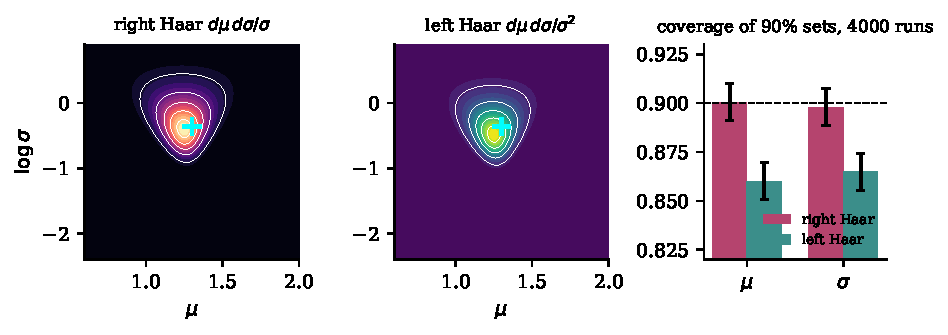
\includegraphics[width=\textwidth]{figs/haar_posterior.pdf}
\caption{Left and centre: right and left Haar posterior densities of $(\mu,\log\sigma)$ for one data set of size $5$ with P\'olya errors; the cross marks the true value $(1.3,\log0.7)$. Right: coverage of $90\%$ equal tailed intervals for $\mu$ and $\sigma$ over $4000$ replications, with bars of two Monte Carlo standard errors; the dashed line is the nominal level.}\label{fig:11bposterior}
\end{figure}

\subsection{Matching and paradoxes}

Theorem~\ref{thm:11bright} makes the right Haar prior an \emph{exact} probability matching prior for $\mu$ and for $\sigma$, stronger than the first order matching of Welch and Peers \cite{welchpeers1963}. Exactness needs only the free action. Optimality needs more: for an invariant loss the Bayes procedure of the right Haar prior is the best equivariant procedure \cite{horabuehler1966,eaton1989}, and by the Hunt Stein theorem the best equivariant procedure is minimax when $G$ is amenable, as the solvable group $B$ is; for the general linear group acting on covariance matrices, which is not amenable, Stein showed that it need not be \cite{eatongeorge2021}.

Dawid, Stone and Zidek \cite{dawidstonezidek1973} showed that improper priors can produce marginalisation paradoxes, in which the posterior of a parameter $\theta$ depends on the data only through a statistic $z$ whose law depends only on $\theta$, and yet no prior on $\theta$ reproduces it from the likelihood of $z$. In group models the paradox is avoided when the prior is right Haar measure on the group that leaves $\theta$ invariant, times any prior on $\theta$. Exercise~\ref{ex:11bparadox} works the classical case $\theta=\mu/\sigma$: here the relevant group is the scale group, the prior free of paradox is $d\mu\,d\sigma/\sigma^2$, and the right Haar prior $d\mu\,d\sigma/\sigma$ of the location scale group produces the paradox. ``Right'' is relative to the group that leaves the parameter of interest invariant; this is the starting point of Chang and Eaves.

\section{Reference priors for orbits}

When the parameter of interest is an orbit of a group acting on the parameter space, reference priors combine Haar measure on the group with a prior on the space of orbits. Conjugacy classes, and hence Satake parameters, are orbits of this kind.

\subsection{Chang and Eaves}

Let $G$ act freely on a parameter space, and let the parameter of interest be the orbit, equivalently a maximal invariant $\theta$. Chang and Eaves \cite{changeaves1990} showed that the prior combining right Haar measure on $G$ with a limiting form of Jeffreys' prior for the maximal invariant coincides with Bernardo's reference prior \cite{bernardo1979,bergerbernardo1992} when the orbit is the parameter of interest. Their prior can be computed without a product parametrisation, and their examples include the correlation matrix and the eigenvalues of a covariance matrix. For a one dimensional maximal invariant, Datta and J. K. Ghosh \cite{dattaghosh1995} compared reference, Chang Eaves and probability matching priors, judged them by marginalisation paradoxes and by frequentist matching, and concluded that the Chang Eaves and Berger Bernardo reference priors are the most attractive; Datta and M. Ghosh \cite{dattaghosh1996} studied which noninformative priors are invariant under reparametrisation.\index{reference prior}

\subsection{Conjugacy classes as orbits}

The Satake parameter of an unramified local representation is a conjugacy class in the dual group, an orbit of the adjoint action; when the representation is tempered it is a class in a compact group $K$, such as a Sato Tate group. We propose (this book) the following model for inference on such a class from noisy group elements. Let $K$ be a compact connected Lie group with Haar probability measure $dh$, let $\varphi\ge0$ be a smooth class function with $\int\varphi\,dh=1$, and observe $Y_1,\dots,Y_n$ independent with density
\begin{equation}\label{eq:11bnoise}
p(y\mid M)=\varphi(M^{-1}y)\quad\text{with respect to }dh,\qquad M=\eta\,t\,\eta^{-1},
\end{equation}
that is $Y=M\varepsilon$ with $\varepsilon$ of density $\varphi$. Examples are the heat kernel $\varphi_s=\sum_\rho\dim\rho\,e^{-sc_\rho}\chi_\rho$ ($c_\rho$ the Casimir eigenvalue) and, for $K=\SU(2)$, the von Mises Fisher law $\varphi(\varepsilon)\propto\exp(\kappa\operatorname{Re}\tr\varepsilon)$. The parameter of interest is the class of $M$, coordinatised by $t$ in a Weyl chamber $T^+$ of a maximal torus $T$; the nuisance parameter is $u=\eta T\in K/T$. Conjugation is not free on $K$, so the theorem of Chang and Eaves does not apply as stated. We instead compute the reference prior directly, with the two group algorithm of Berger and Bernardo \cite{bergerbernardo1992}, ordered as (class, conjugator): on a compact parameter space with information matrix $I=\bigl(\begin{smallmatrix}I_{11}&I_{12}\\I_{21}&I_{22}\end{smallmatrix}\bigr)$,
\begin{equation}\label{eq:11bbb}
\pi(u\mid t)\propto|I_{22}(t,u)|^{1/2},\qquad \pi(t)\propto\exp\Bigl\{\int\pi(u\mid t)\log|I_{11\cdot2}(t,u)|^{1/2}\,du\Bigr\},
\end{equation}
with $I_{11\cdot2}=I_{11}-I_{12}I_{22}^{-1}I_{21}$.

\begin{proposition}[this book]\label{thm:11brefprior}
Let $K$ be compact, connected and simple, and suppose the Fisher information of \eqref{eq:11bnoise} at $M=e$ is finite and nonsingular. Then:
\begin{enumerate}
\item[(i)] The Fisher metric is $c\,n$ times a fixed bi invariant Riemannian metric on $K$, for a constant $c=c(\varphi)>0$; Jeffreys' prior for $M$ is Haar measure, and its image on classes has the Weyl density $|W|^{-1}\prod_{\alpha}|e^{i\alpha(t)}-1|$ (product over all roots) with respect to the Haar probability measure $dt$ of $T$: it is the Sato Tate measure of $K$.
\item[(ii)] The reference prior \eqref{eq:11bbb} is the product of the $K$ invariant probability measure on $K/T$ and the uniform (Haar) measure $dt$ on the Weyl chamber. Its image on classes is the image of Haar measure on the torus $T$.
\end{enumerate}
For $K=\SU(2)$ the reference prior for the angle $\theta\in[0,\pi]$ is $d\theta/\pi$, so $x=2\cos\theta$ has the arcsine law, against the Sato Tate prior $\frac2\pi\sin^2\theta\,d\theta$. For $K=\USp(4)$ it is uniform on $0\le\theta_2\le\theta_1\le\pi$, against the density proportional to $(\cos\theta_1-\cos\theta_2)^2\sin^2\theta_1\sin^2\theta_2$ of Proposition~\ref{thm:12usp4}.
\end{proposition}

\begin{proof}
(i) The group $K\times K$ acts on parameters and data by $(g_1,g_2)\cdot M=g_1Mg_2^{-1}$, $(g_1,g_2)\cdot y=g_1yg_2^{-1}$, preserving $dh$, and $p(g_1yg_2^{-1}\mid g_1Mg_2^{-1})=\varphi(g_2M^{-1}yg_2^{-1})=\varphi(M^{-1}y)$ because $\varphi$ is a class function. So the Fisher metric is invariant under left and right translations. At $e$ it is an $\operatorname{Ad}(K)$ invariant inner product on the Lie algebra $\mathfrak k$, and since $K$ is simple $\operatorname{Ad}$ is irreducible, so by Schur's lemma the inner product is a multiple $c$ of a fixed invariant one; $c>0$ by the nonsingularity assumption, and independence multiplies it by $n$. The Riemannian volume of a bi invariant metric is Haar measure, and the image on classes is given by Weyl's integration formula.

(ii) On the regular set write $M=\eta t\eta^{-1}$ with $t$ in the interior of the Weyl chamber; since the centraliser of a regular $t$ is $T$, the map $(\eta T,t)\mapsto M$ is a diffeomorphism onto the regular set, whose complement has Haar measure zero. For $Y\in\mathfrak t$ the tangent vector $\frac{d}{ds}\eta te^{sY}\eta^{-1}$ is the left translate by $\eta t\eta^{-1}$ of $\operatorname{Ad}(\eta)Y$; for $X\in\mathfrak t^\perp$, $\frac{d}{ds}\eta e^{sX}te^{-sX}\eta^{-1}$ is the left translate of $\operatorname{Ad}(\eta)(\operatorname{Ad}(t^{-1})X-X)$. The bi invariant metric is $\operatorname{Ad}$ invariant, $\mathfrak t^\perp$ is $\operatorname{Ad}(t)$ stable, so torus and orbit directions are orthogonal: $I_{12}=0$ and $I_{11\cdot2}=I_{11}=cn\,\|\cdot\|^2_{\mathfrak t}$, constant in $(t,u)$. On a root plane $\mathfrak k_\alpha\subset\mathfrak t^\perp$, $\operatorname{Ad}(t^{-1})$ is a rotation by the angle $\alpha(t)$, so $\|\operatorname{Ad}(t^{-1})X-X\|=|e^{i\alpha(t)}-1|\,\|X\|$, and therefore $|I_{22}(t,u)|^{1/2}=(cn)^{\dim K/T/2}\prod_{\alpha>0}|e^{i\alpha(t)}-1|^2\,v(u)$, with $v$ the density of the invariant volume of $K/T$. In \eqref{eq:11bbb}, normalising over $u\in K/T$ removes the factor depending on $t$, so $\pi(u\mid t)$ is the invariant probability on $K/T$; and $I_{11\cdot2}$ is constant, so $\pi(t)$ is uniform. The image of $dt$ on $T^+=T/W$ is the image of Haar measure on $T$. For $\SU(2)$ the chamber is $\theta\in[0,\pi]$, and for $\USp(4)$, $W$ is generated by sign changes and the swap, with chamber $0\le\theta_2\le\theta_1\le\pi$.
\end{proof}

Proposition~\ref{thm:11brefprior} splits Weyl's formula into two parts. The Vandermonde factor $\prod_\alpha|e^{i\alpha}-1|$ is the volume of the conjugacy orbit, nuisance information about the conjugator, and the reference prior removes it. The result agrees with the formal Chang Eaves recipe: Haar measure on the conjugating group times Jeffreys' prior for $t$ with $\eta$ known, which is uniform because $I_{11}$ is constant. The two priors on classes of $\SU(2)$ are far apart: by Lemma~\ref{thm:12integral},
\[
\mathrm{KL}\Bigl(\frac{d\theta}{\pi}\Big\|\frac2\pi\sin^2\theta\,d\theta\Bigr)=\log2,\qquad\mathrm{KL}\Bigl(\frac2\pi\sin^2\theta\,d\theta\Big\|\frac{d\theta}{\pi}\Bigr)=1-\log2,
\]
using $\int_0^\pi\log\sin\theta\,d\theta=-\pi\log2$. The reference prior is the normalised continuous part of the law $\mu_{\mathrm{CM}}$ of Chapter~\ref{ch:04}: the reference prior for a class of $\SU(2)$ is the Sato Tate law of the torus. Which prior to use depends on the question. For the class of a single Frobenius element of a curve without complex multiplication, the Sato Tate law is the correct prior. For the class of an unknown group element observed through isotropic noise, with no arithmetic information, the reference prior is uniform on the torus. Anisotropic noise, or an unknown noise level, breaks the block structure and is left as Computational Problem~\ref{cp:11bchangeaves}.

\section{Haar measure behind L values}\label{sec:11btamagawa}

Haar measures normalise the volumes in special value formulas; we record three instances without proofs.\index{Tamagawa number}

\emph{Volumes and zeta values.} With $dx\,dy/y^2$, $\operatorname{vol}(\SL_2(\Z)\backslash\mathbb H)=\pi/3=2\zeta(2)/\pi$ by \eqref{eq:11barea}. More generally, with Haar measure on $\SL_n(\R)$ normalised through Lebesgue measure on matrices, $\operatorname{vol}(\SL_n(\Z)\backslash\SL_n(\R))=\zeta(2)\zeta(3)\cdots\zeta(n)$; this goes back to Minkowski and was proved by Siegel \cite{siegel1945}, whose analytic theory of quadratic forms, including the average measure of \cite{siegel1944}, led to the Siegel Weil formula.

\emph{Tamagawa numbers.} For a semisimple group $H$ over $\Q$, an invariant differential form of top degree defines Haar measures on every $H(\Q_v)$; their product is a measure on $H(\A)$ independent of the form by the product formula, and $\tau(H)=\operatorname{vol}(H(\Q)\backslash H(\A))$. Weil proved $\tau(\SL_2)=1$ \cite{weil1961}. The mechanism is visible in a sketch. Strong approximation gives
\[
\SL_2(\Q)\backslash\SL_2(\A)=\SL_2(\Z)\backslash\Bigl(\SL_2(\R)\times\prod_p\SL_2(\Z_p)\Bigr),
\]
so $\tau(\SL_2)$ is the product of the archimedean volume $\operatorname{vol}(\SL_2(\Z)\backslash\SL_2(\R))=\zeta(2)$ and the volumes $\#\SL_2(\mathbb F_p)/p^3=1-p^{-2}$ of the groups $\SL_2(\Z_p)$, all for the form measure; since $\prod_p(1-p^{-2})=\zeta(2)^{-1}$, the product is $1$.

\emph{Period formulas.} Waldspurger's formula \cite{waldspurger1985} expresses the square of a toric period of a $\GL_2$ automorphic form, for example a Weyl sum over Heegner points, as a central value $L(\frac12,\pi_K)$ divided by $L(1,\pi,\operatorname{Ad})$, times local factors. Ichino and Ikeda \cite{ichinoikeda2010} formulated the analogue for $\mathrm{SO}(n+1)\times\mathrm{SO}(n)$ periods, as a refinement of the Gross Prasad conjecture, and verified it in low rank cases. In both, the global constant is fixed only once Tamagawa measures are chosen on the groups and their subgroups, and each local factor is an integral of matrix coefficients against local Haar measure. The Duke computation of Section~\ref{sec:11bduke} is the case where all these normalisations are hidden in $\frac3\pi$.

\section{Notes}

The Iwasawa integration formula and the half plane are treated in \cite{bump1997}. Fisher's conditional argument for location and scale is \cite{fisher1934} and his fiducial argument \cite{fisher1935}; structural inference is Fraser's \cite{fraser1968}. The $p^*$ formula, its exactness for transformation models and its accuracy elsewhere are due to Barndorff Nielsen \cite{barndorffnielsen1980,barndorffnielsen1983}, with the systematic treatment in \cite{barndorffnielsencox1994} and the survey \cite{reid1988}; the saddlepoint method is Daniels' \cite{daniels1954}. Stein \cite{stein1965} and Hora and Buehler \cite{horabuehler1966} identified Bayes procedures under right Haar priors with best invariant procedures and fiducial distributions; Eaton's lectures \cite{eaton1989} give the general theory of group invariance in statistics and Berger \cite{berger1985} the decision theoretic setting; Eaton and George \cite{eatongeorge2021} trace Stein's work on invariance from the Hunt Stein theorem to his counterexamples for groups that are not amenable. Marginalisation paradoxes are from \cite{dawidstonezidek1973}; reference priors from \cite{bernardo1979,bergerbernardo1992}, and for orbits from Chang and Eaves \cite{changeaves1990}, compared by Datta and J. K. Ghosh \cite{dattaghosh1995}; Datta and M. Ghosh \cite{dattaghosh1996} treat their invariance. Duke's theorem is \cite{duke1988}, building on Iwaniec \cite{iwaniec1987}, with Waldspurger's formulas \cite{waldspurger1981,waldspurger1985} giving the $L$ function interpretation; Linnik's ergodic method is in \cite{linnik1968}. Proposition~\ref{thm:11bhyperbolic} and Theorems~\ref{thm:11bpstar} and \ref{thm:11bright} are classical; only the proofs of the two theorems in the generality of Definition~\ref{def:11bmodel} are written for this book. Ours are Proposition~\ref{thm:11brefprior}, the exact normal coverages of Section~\ref{sec:11bright} and the computations, all elementary consequences of the cited theory.

\section{Exercises}

\begin{enumerate}
\item Verify Proposition~\ref{thm:11baffine} through Lemma~\ref{thm:11bleftright}: compute $\operatorname{Ad}(a,b)$ on the Lie algebra of $B$ in the basis $\bigl(\begin{smallmatrix}1&0\\0&0\end{smallmatrix}\bigr)$, $\bigl(\begin{smallmatrix}0&1\\0&0\end{smallmatrix}\bigr)$, and check $\Delta_B=|\det\operatorname{Ad}|^{-1}=a^{-1}$. Show that no nonzero Radon measure on $\R$ is invariant under all the maps $x\mapsto ax+b$, although $B$ acts transitively on $\R$.
\item\label{ex:11bborel} For the Borel subgroup of $\GL_2(F)$, $F=\R$ or $\Q_p$, prove that
\[d\mu_l=|a|^{-2}|d|^{-1}da\,db\,dd,\qquad d\mu_r=|a|^{-1}|d|^{-2}da\,db\,dd\]
and $\Delta_{B_2}=|d/a|$. Check that $\Delta_{B_2}$ is trivial on the unipotent radical and on the centre.
\item Show that for the normal location scale model $p^*$ is exact without conditioning, by computing $j(\hat\mu,\hat\sigma)=\operatorname{diag}(n,2n)/\hat\sigma^2$ and comparing \eqref{eq:11bpstar} with the joint density of $\bar X$ and $\hat\sigma^2=S/n$, using independence and $S/\sigma^2\sim\chi^2_{n-1}$. Identify the constant $c$.
\item Compute the hyperbolic area of the fundamental domain of $\Gamma_0(2)$ by showing that it is the union of $[\SL_2(\Z):\Gamma_0(2)]=3$ translates of $\mathcal F$, and of $\Gamma_0(p)$ in general. Derive \eqref{eq:11barea} also from the Gauss Bonnet formula for the triangle with angles $\pi/3$, $\pi/3$, $0$.
\item\label{ex:11bclass} Let $D<-4$ be a fundamental discriminant. Show that $Q\mapsto z_Q$ is injective, that $\SL_2(\Z)$ equivalence of forms corresponds to the action on roots, and that each class of primitive positive definite forms of discriminant $D$ contains exactly one reduced form; deduce that $\#\Lambda_D=h(D)$. Show that $\operatorname{Im}z_Q=\sqrt{|D|}/(2a)$, so that $\operatorname{Im}z_Q>t$ if and only if $a<\sqrt{|D|}/(2t)$, and use this to compute the tail counts of Table~\ref{tab:11bduke} from the list of reduced forms.
\item\label{ex:11bparadox} (Marginalisation paradox.) Let $X_1,\dots,X_n$ be independent $N(\mu,\sigma^2)$, $\theta=\mu/\sigma$, $T=\sum X_i^2$, $U=\sum X_i$, $z=U/\sqrt T$, and take the prior $\sigma^{-r}d\mu\,d\sigma$. Show that the posterior of $\theta$ is proportional to
\[e^{-n\theta^2/2}\int_0^\infty v^{n+r-3}e^{-v^2/2+\theta zv}dv,\]
which depends on the data only through $z$, and that the law of $z$ has density proportional to $(1-z^2/n)^{(n-3)/2}e^{-n\theta^2/2}\int_0^\infty v^{n-1}e^{-v^2/2+\theta zv}dv$. Conclude that a prior $\pi(\theta)$ reproduces the first posterior from the law of $z$ if and only if $r=2$, and observe that $d\mu\,d\sigma/\sigma^2=d\theta\,d\sigma/\sigma$ is Lebesgue measure in $\theta$ times the Haar measure $d\sigma/\sigma$ of the scale group $x\mapsto cx$, $c>0$, which leaves $\theta$ and $z$ invariant.
\end{enumerate}

\section{Open computational problems}

\begin{compproblem}[Duke rates at large discriminant]\label{cp:11bduke}
Objective: measure the rate in Theorem~\ref{thm:11bduke}. Objects: Heegner points for all fundamental discriminants with $|D|\le10^9$, and for samples of discriminants near $10^{10}$, $10^{11}$ and $10^{12}$ (class numbers up to about $10^6$). Route: enumerate reduced forms with PARI/GP \texttt{qfbred} and \texttt{qfbclassno} on a cluster, or generate the class group from prime forms with GPU batch reduction. Deliverable: the discrepancy of $\Lambda_D$ against $\frac3\pi dx\,dy/y^2$ over hyperbolic disks and over the tail sets $\operatorname{Im}z>t$, and the Weyl sums of the first ten Maass cusp forms (from the LMFDB), with fitted exponents $\delta$ in $|D|^{-\delta}$. Why it matters: Waldspurger's formula turns the Weyl sums into central $L$ values, so the fitted exponents test the subconvexity input and the Lindel\"of prediction $\delta=\frac14$ for the cusp form sums.
\end{compproblem}

\begin{compproblem}[Reference priors for anisotropic noise]\label{cp:11bchangeaves}
Objective: extend Proposition~\ref{thm:11brefprior} beyond bi invariant noise. Objects: $\SU(2)$ and $\USp(4)$ with matrix Fisher noise $\varphi(\varepsilon)\propto\exp(\operatorname{Re}\tr(F\varepsilon))$ for nonscalar $F$, and the heat kernel $\varphi_s$ with the time $s$ unknown. Route: Fisher information by Weyl integration and Gauss quadrature on the torus, then the Berger Bernardo algorithm with the class first, and the Chang Eaves recipe with right Haar measure on the stabiliser free part. Deliverable: the reference prior on classes as a density on the Weyl chamber, its Kullback Leibler distance to the Weyl density and to the torus Haar measure, and frequentist coverage of reference posterior sets for the class at $n=5,20,100$. Why it matters: it decides whether the Vandermonde factor of the Sato Tate measure survives in objective inference on Satake parameters when the noise is not symmetric.
\end{compproblem}

\begin{compproblem}[p* and right Haar intervals for angular models]\label{cp:11bpstar}
Objective: measure what the group structure buys for $p^*$ and for Haar priors in models built from Sato Tate data. Objects: the location and scale models $x_i=\mu+\sigma\varepsilon_i$ with $\varepsilon_i$ distributed by $\ST$, by the $\USp(4)$ trace law and by $\Phi_\Delta$; the von Mises model on the circle with unknown rotation, a group model, and with unknown rotation and concentration, a full exponential family that is not a group model; $n$ from $5$ to $200$. Route: exact conditional densities and constants $c(a)$ from Theorem~\ref{thm:11bpstar} by quadrature over the group, exact and saddlepoint densities for the two parameter von Mises model, and $10^5$ replications per setting in vectorised code. Deliverable: tables of the ratio $(2\pi)^{-d/2}/c(a)$ of unnormalised $p^*$ to the exact conditional density, as a function of $n$ and of the configuration; of the relative error of renormalised $p^*$ in the two parameter von Mises model; and of the coverage of right and left Haar intervals. Why it matters: in the group models renormalised $p^*$ and right Haar intervals are exact whatever the error law (Theorems~\ref{thm:11bpstar} and \ref{thm:11bright}), but the accuracy of the unnormalised formula rests on Laplace's method. The $\USp(4)$ trace density vanishes to fourth order at $\pm4$ and $\Phi_\Delta$ is smooth, so those models are regular, while the semicircle vanishes like a square root at $\pm2$ and has infinite Fisher information for location; the tables show whether the $O(n^{-1})$ accuracy of the constant survives in this nonregular model, and how the exact group answers compare with the $O(n^{-3/2})$ approximation outside group models.
\end{compproblem}

\begin{compproblem}[CM points and Hecke orbits on Shimura curves]\label{cp:11bshimura}
Objective: test equidistribution for Haar measure on compact quotients of $\mathbb H$. Objects: the Shimura curves attached to the maximal orders of the quaternion algebras over $\Q$ of discriminant $6$, $10$ and $14$; CM points of discriminant $|D|\le10^8$, and Hecke orbits $T_{p^k}x$ for the primes $p\le7$ not dividing the discriminant and $p^k\le10^7$. Route: Magma or Sage quaternion arithmetic for optimal embeddings, explicit fundamental domains (Voight's algorithms) for the hyperbolic coordinates. Deliverable: discrepancy against the normalised hyperbolic area, the decay rate in $|D|$ and in $p^k$, and for Hecke orbits a comparison with the rate $(k+1)p^{-k/2}$ that the Ramanujan conjecture for the Maass forms of the curve predicts (the random walk generated by $T_p$ has the corresponding Kesten rate $(2\sqrt p/(p+1))^k$ of Chapter~\ref{ch:07}). Why it matters: there is no cusp here, so the noncompact effects of Table~\ref{tab:11bduke} disappear; Hecke orbits are images of the Bruhat Tits tree of $\PGL_2(\Q_p)$ in the curve, which joins Chapter~\ref{ch:07} to the invariant measure of this chapter, and their decay rate is a numerical test of the Ramanujan conjecture for Maass forms, which is open.
\end{compproblem}

\chapter{Bayesian Identification of Sato Tate Groups}\label{ch:12}

When Fit\'e, Kedlaya, Rotger and Sutherland classified the Sato Tate groups of abelian surfaces they did two things at once: they proved that exactly $52$ compact groups occur, up to conjugacy in $\USp(4)$, as Sato Tate groups of abelian surfaces over number fields, and they matched curves to groups by comparing empirical moments of the normalised $L$ polynomial coefficients with the moments of each candidate \cite{fkrs2012}. The second activity is statistical inference, though it is rarely described that way. This chapter makes the inference explicit: the data are the normalised traces $x_p$, the parameter is a compact group $G$, and the model is the image of Haar measure on $G$ under the trace. Bayes factors computed from this working model are consistent, with rates given by Kullback Leibler divergences, as a deterministic theorem about the actual traces whenever they are equidistributed for the true law, atoms included, and that law has finite divergence from a candidate (Theorem~\ref{thm:12consist}). We test the procedure on three genus $2$ curves, one of which lies outside the candidate set, and use that failure to argue for the full $52$ group likelihood.

\section{The inference problem}

Let $A/\Q$ be an abelian variety of dimension $g$ with good reduction outside $N$. For $p\nmid N$ the normalised Frobenius $s_p$ is a conjugacy class of the Sato Tate group $G=\mathrm{ST}(A)\subset\USp(2g)$, and the general Sato Tate conjecture (Conjecture~\ref{conj:ch3gst}) asserts that $(s_p)$ is equidistributed for the image $\mu_G$ of Haar measure. We observe $x_p=a_p/\sqrt p=\tr s_p\in[-2g,2g]$. Given $x_{p_1},\dots,x_{p_n}$, which $G$?\index{Sato Tate group}

For elliptic curves ($\SU(2)$ or $N(\mathrm{U}(1))$) complex multiplication is cheap to detect directly, but the statistical answer is the template for higher genus, where the candidates are many.

\section{Exchangeability as a working model}

The traces are determined by the curve, so a likelihood for them is a working model.\index{exchangeability} By de Finetti's theorem \cite{definetti1937,hewittsavage1955} an infinite exchangeable sequence is a mixture of independent and identically distributed sequences, so to model $(x_p)$ as exchangeable is to model it as an independent sample from an unknown law with a prior on that law. Here the prior is supported on the finitely many laws $\mu_G$, and the posterior over $G$ is the posterior over the de Finetti measure. A frequentist reading of the same likelihood is a working model in the same sense.

The only property of independent sampling used by the first order asymptotics of Bayes factors, their exponential rates, is the strong law of large numbers for the log likelihood ratio. For arithmetic data it is replaced by equidistribution, $n^{-1}\sum_{k\le n}\varphi(x_{p_k})\to\int\varphi\,d\mu_G$ for continuous $\varphi$, which plays the role of the ergodic theorem. It does not supply independence, so finite sample error probabilities are calibrated only insofar as the traces fluctuate like random ones, as Chapter~\ref{ch:05} suggests they do. Proposition~\ref{prop:01limits} gives the limitation: equidistribution is blind to alterations on sets of density zero, and so is every limit in this chapter.

\section{A general consistency theorem}

Fix a compact set $K\subset\R$, a finite set $D\subset K$, and the reference measure $\nu$ equal to Lebesgue measure on $K$ plus counting measure on $D$. Candidate laws $P_0,P_1$ and the true law $\mu_0$ have $\nu$ densities $f_0,f_1,m$, so their atoms lie in $D$. Write $h=\log(f_1/f_0)$, with values in $[-\infty,\infty]$, and for a clipping level $M>0$ write $h_M=\max(-M,\min(M,h))$. For a deterministic sequence $(x_k)$ in $K$ define the clipped log Bayes factor
\[
\log B_n^M=\sum_{k\le n}h_M(x_k).
\]
We say that $(x_k)$ is \emph{equidistributed for $\mu_0$ relative to $D$} if $n^{-1}\#\{k\le n:x_k=a\}\to\mu_0(\{a\})$ for each $a\in D$ and $n^{-1}\sum_{k\le n,\,x_k\notin D}\delta_{x_k}$ converges weakly to the restriction of $\mu_0$ to $K\setminus D$. When $\mu_0$ has no atoms this follows from equidistribution by the portmanteau theorem.

\begin{theorem}[Consistency under equidistribution; this book]\label{thm:12consist}
Suppose $(x_k)$ is equidistributed for $\mu_0$ relative to $D$, that $h$ is finite on $D$, that on $K\setminus D$ the function $h$ agrees almost everywhere with a continuous map $\tilde h:K\to[-\infty,\infty]$, through which $h$ is evaluated off $D$, and that $\mathrm{KL}(\mu_0\|P_0)<\infty$. Then for every $M$,
\[
\lim_{n\to\infty}\frac1n\log B_n^M=\int h_M\,d\mu_0,
\]
and as $M\to\infty$ the right side tends to
\[
\int h\,d\mu_0=\mathrm{KL}(\mu_0\|P_0)-\mathrm{KL}(\mu_0\|P_1)\in[-\infty,\infty).
\]
In particular, if $\mu_0=P_0$ the double limit is $-\mathrm{KL}(P_0\|P_1)$.
\end{theorem}

\begin{proof}
Divide by $n$ and split the sum according to whether $x_k\in D$. The first part is
\[
\sum_{a\in D}h_M(a)\,\frac{\#\{k\le n:x_k=a\}}n\longrightarrow\sum_{a\in D}h_M(a)\,\mu_0(\{a\}).
\]
On the second part $h_M=\tilde h_M$, a bounded continuous function on $K$, so weak convergence gives the limit $\int_{K\setminus D}\tilde h_M\,d\mu_0=\int_{K\setminus D}h_M\,d\mu_0$. Adding proves the first claim.

For the second, write $h_M=\min(h^+,M)-\min(h^-,M)$; by monotone convergence the integrals increase to those of $h^\pm$, and it suffices that $\int h^+d\mu_0<\infty$. Since $\mathrm{KL}(\mu_0\|P_0)<\infty$, $f_0>0$ almost everywhere for $\mu_0$, and on $\{m>0\}$ we have $h=\log(f_1/m)+\log(m/f_0)$. Since $\log y\le y$,
\[
\int\Bigl(\log\frac{f_1}{m}\Bigr)^+d\mu_0\le\int f_1\,d\nu=1,\qquad\int\Bigl(\log\frac{m}{f_0}\Bigr)^-d\mu_0\le\int f_0\,d\nu=1,
\]
so $\int|\log(m/f_0)|\,d\mu_0\le\mathrm{KL}(\mu_0\|P_0)+2<\infty$. Hence $h^+$ is integrable and $\int h\,d\mu_0=-\mathrm{KL}(\mu_0\|P_1)+\mathrm{KL}(\mu_0\|P_0)$.
\end{proof}

When the truth is one of the two candidates the rate is a single divergence, up to sign; in general it is a difference of two, as in the case without complex multiplication below, where $\mu_0=\ST$ is not the candidate $M_{\mathrm{ST}}$. Clipping lets weak convergence act on $h$, which may be unbounded; the independent version in Appendix~\ref{app:A} rests on the strong law of large numbers and needs no clipping.\index{Bayes factor}\index{Kullback Leibler divergence}

\section{Elliptic curves: the constants}

With $D=\{0\}$ the models are $M_{\mathrm{ST}}:x_p\sim(1-\varepsilon)\ST+\varepsilon\delta_0$ and $M_{\mathrm{CM}}:x_p\sim\mu_{\mathrm{CM}}=\frac12\delta_0+\frac12\,\mathrm{arcsine}$, where the arcsine law on $[-2,2]$ has density $(\pi\sqrt{4-x^2})^{-1}$. The small atom $\varepsilon$ keeps a single supersingular prime from being decisive; curves without complex multiplication have infinitely many of them \cite{elkies1987}. The log likelihood ratio of $M_{\mathrm{CM}}$ to $M_{\mathrm{ST}}$ is
\[
h(x)=-\log(1-\varepsilon)-\log(4-x^2)\quad(x\neq0),\qquad h(0)=\log\frac1{2\varepsilon},
\]
since $\frac12(\pi\sqrt{4-x^2})^{-1}$ divided by $(1-\varepsilon)(2\pi)^{-1}\sqrt{4-x^2}$ is $((1-\varepsilon)(4-x^2))^{-1}$. Off $D$ it extends continuously to $[-2,2]$ with values in $(-\infty,\infty]$.

\begin{lemma}\label{thm:12integral}
$\int_0^\pi\sin^2\theta\log\sin\theta\,d\theta=\frac\pi4(1-2\log2)$. Consequently
\[
\int\log(4-x^2)\,d\ST=1,\qquad \int_{-2}^2\log(4-x^2)\,\frac{dx}{\pi\sqrt{4-x^2}}=0.
\]
\end{lemma}

\begin{proof}
On $(0,\pi)$, $\log\sin\theta=-\log2-\sum_{k\ge1}k^{-1}\cos2k\theta$, with convergence in $L^2$. Multiply by $\sin^2\theta=\frac12(1-\cos2\theta)$ and integrate: $\int_0^\pi\cos2k\theta\,d\theta=0$ and $\int_0^\pi\cos2\theta\cos2k\theta\,d\theta=\frac\pi2$ if $k=1$ and $0$ otherwise. The constant term contributes $-\frac\pi2\log2$ and the $k=1$ term contributes $\frac\pi4$, which gives the first formula. With $x=2\cos\theta$ we have $\log(4-x^2)=\log4+2\log\sin\theta$, and $\ST$ becomes $\frac2\pi\sin^2\theta\,d\theta$ on $[0,\pi]$, so $\int\log(4-x^2)\,d\ST=\log4+\frac4\pi\cdot\frac\pi4(1-2\log2)=1$. Under the arcsine law $\theta$ is uniform and the constant term alone survives: $\log4+\frac2\pi(-\pi\log2)=0$.
\end{proof}

\begin{corollary}[Rates for elliptic curves; this book]\label{thm:12elliptic}
Let $E/\Q$ be an elliptic curve and $0<\varepsilon<\frac12$. If $E$ has no complex multiplication, $\lim_M\lim_n n^{-1}\log B_n^M=-1-\log(1-\varepsilon)$. If $E$ has complex multiplication, the limit is $\frac12\log\frac1{2\varepsilon}-\frac12\log(1-\varepsilon)>0$.
\end{corollary}

\begin{proof}
Without complex multiplication $(x_p)$ is $\ST$ equidistributed by Theorem~\ref{thm:04STthm}, hence equidistributed for $\ST$ relative to $\{0\}$. Apply Theorem~\ref{thm:12consist} with $\mu_0=\ST$, $P_0=M_{\mathrm{ST}}$ and $P_1=\mu_{\mathrm{CM}}$: here $\mathrm{KL}(\ST\|M_{\mathrm{ST}})=-\log(1-\varepsilon)$, and $\mathrm{KL}(\ST\|\mu_{\mathrm{CM}})=\int\log(4-x^2)\,d\ST=1$ by Lemma~\ref{thm:12integral}. With complex multiplication, $(x_p)$ is equidistributed for $\mu_{\mathrm{CM}}$ (Section~\ref{sec:04cm}), and relative to $\{0\}$, because $a_p=0$ at the good primes inert in the CM field, which have density $\frac12$, while $a_p\neq0$ at the split primes of good reduction, which are ordinary. Now $\mu_0=P_1$, and by the arcsine half of Lemma~\ref{thm:12integral} the limit is
\[
\mathrm{KL}(\mu_{\mathrm{CM}}\|M_{\mathrm{ST}})=\frac12\log\frac{1/2}{\varepsilon}+\frac12\bigl(-\log(1-\varepsilon)-0\bigr).\qedhere
\]
\end{proof}

With $\varepsilon=10^{-3}$ and $M=20$ the theoretical rates are $-0.999$ and $3.108$ nats per prime. For $E_1:y^2=x^3+x+1$ (conductor $496$, no complex multiplication) and $E_2:y^2=x^3-x$ (complex multiplication by $\Z[i]$) over the good primes below $40000$ we observed $-0.979$ and $3.102$; after only $50$ primes $\log B=-15.9$ and $+160.4$ respectively (Figure~\ref{fig:12bayes}). The slow start for $E_1$ comes from its supersingular primes $3$, $17$, $179$ and $227$ among the first $50$, each of which adds $\log(1/(2\varepsilon))=6.21$ instead of about $-1$. The CM decision is faster because half the primes give $a_p=0$, which $M_{\mathrm{ST}}$ scores as probability $\varepsilon$.

\begin{figure}[htbp]\centering
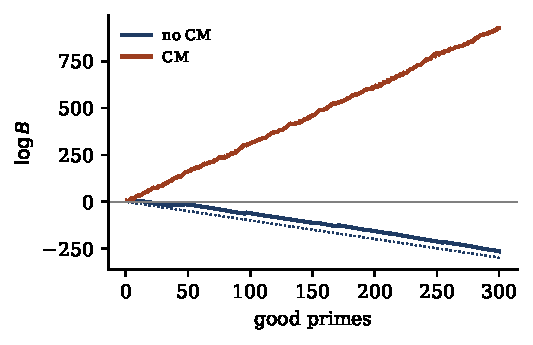
\includegraphics[width=0.62\textwidth]{figs/bayes.pdf}
\caption{Log Bayes factor of $M_{\mathrm{CM}}$ against $M_{\mathrm{ST}}$ over the first $300$ good primes for $E_1:y^2=x^3+x+1$ (no complex multiplication) and $E_2:y^2=x^3-x$ (complex multiplication), with $\varepsilon=10^{-3}$ and clipping at $M=20$. Dotted lines: the limiting slopes $-0.999$ and $3.108$ of Corollary~\ref{thm:12elliptic}.}\label{fig:12bayes}
\end{figure}

\section{Sequential testing}

Wald's sequential probability ratio test \cite{wald1947} of $P_0$ against $P_1$ stops when $\log B_n$ leaves the interval
\[
\Bigl(\log\frac{\beta}{1-\alpha},\ \log\frac{1-\beta}{\alpha}\Bigr),
\]
where $\alpha$ and $\beta$ are the target probabilities of rejecting $P_0$ when it holds and of accepting it when $P_1$ holds.\index{sequential probability ratio test} For independent observations Wald and Wolfowitz proved that no test whose error probabilities are at most those of the sequential probability ratio test has a smaller expected sample size under either hypothesis \cite{waldwolfowitz1948}, and Wald's identity, ignoring overshoot, gives $\E_1[N]\approx\log(1/\alpha)/\mathrm{KL}(P_1\|P_0)$ for small $\alpha,\beta$. By Theorem~\ref{thm:12consist} the arithmetic walk $\log B_n$ drifts at the rate computed there, so the same count, with that rate in place of the divergence, describes the actual traces as $\alpha,\beta\to0$; the error probabilities themselves come only from the working model. With $\alpha=\beta=10^{-6}$ and the rates of Corollary~\ref{thm:12elliptic}, the count is $13.8$ primes without complex multiplication and $4.4$ with it; on the actual traces the test stops at the $29$th good prime for $E_1$, delayed by the supersingular primes $3$ and $17$, and at the $4$th for $E_2$. In genus $2$ the divergences of Table~\ref{tab:12kl} are as small as $0.117$, and the approximation asks for about $120$ primes.

\section{Moments versus likelihood}

Moments are linear combinations of the Weyl averages
\[
W_\rho(n)=\frac1n\sum_{k\le n}\chi_\rho(s_{p_k}),
\]
with $\rho$ running over the irreducible representations of $\USp(2g)$, and the vector $(\int\chi_\rho\,d\mu_G)_\rho$ is the Weyl fingerprint of $G$.\index{Weyl fingerprint} If the log likelihood ratio has a uniformly convergent Peter Weyl expansion $h=\sum_\rho c_\rho\chi_\rho$, then
\[
\frac1n\log B_n=\sum_\rho c_\rho\,W_\rho(n).
\]
The log Bayes factor is a linear functional of the Weyl averages, so the vector of Weyl averages is sufficient in the limit: sequences with the same limiting fingerprint have the same Bayes factor rates for every pair of candidates. The likelihood chooses the weights $c_\rho$ optimally (Neyman Pearson); matching a few moments is valid but inefficient. In genus $2$ the conjugacy class of $s_p$ in $\USp(4)$ is determined by the normalised coefficients $(a_1,a_2)$ of the $L$ polynomial, and the trace $a_1$ alone loses information: the $55$ candidate groups of \cite{fkrs2012}, of which $52$ occur, give only $37$ distinct laws of $a_1$, while the laws of $a_1$ and of $a_2$ together distinguish all of them. No trace likelihood separates two groups with the same law of $a_1$.

\section{Genus two: three connected candidates}

We compare three connected groups through their trace laws on $[-4,4]$. Write $s(x)=(2\pi)^{-1}\sqrt{4-x^2}$ for the semicircle density.

\begin{proposition}[Weyl integration on $\USp(4)$]\label{thm:12usp4}
A class function $\varphi$ on $\USp(4)$, written in terms of the eigenvalue angles $e^{\pm i\theta_1},e^{\pm i\theta_2}$, satisfies, for the Haar probability measure $dh$,
\[
\int_{\USp(4)}\varphi\,dh=\frac8{\pi^2}\int_{[0,\pi]^2}\varphi\,(\cos\theta_1-\cos\theta_2)^2\sin^2\theta_1\sin^2\theta_2\,d\theta_1\,d\theta_2 .
\]
So $x_i=2\cos\theta_i$ have joint density $\frac12(x_1-x_2)^2s(x_1)s(x_2)$, and $t=x_1+x_2$ has density
\[
f_{\USp(4)}(t)=\frac12\int(2x-t)^2s(x)s(t-x)\,dx,\qquad f_{\USp(4)}(0)=\frac{64}{15\pi^2},
\]
with even moments $1,3,14$.
\end{proposition}

\begin{proof}
The first display is the case $g=2$ of the density \eqref{eq:ch6usp}, a consequence of Theorem~\ref{thm:ch6weyl}; its constant is $2^4/(2!\,\pi^2)=8/\pi^2$. The change of variables uses $s(x)\,dx=\frac2\pi\sin^2\theta\,d\theta$ and $(x_1-x_2)^2=4(\cos\theta_1-\cos\theta_2)^2$. At $t=0$,
\[
f(0)=2\int x^2s(x)^2\,dx=\frac{1}{2\pi^2}\int_{-2}^2(4x^2-x^4)\,dx=\frac{64}{15\pi^2},
\]
and, for independent semicircular $x_1,x_2$,
\[
\E_{\USp(4)}t^2=\tfrac12\E\bigl[(x_1+x_2)^2(x_1-x_2)^2\bigr]=\E x_1^4-(\E x_1^2)^2=1;
\]
the other moments are similar.
\end{proof}

The second candidate, $\SU(2)\times\SU(2)$ embedded block diagonally, has trace density $s*s$ (value $8/(3\pi^2)$ at $0$, moments $2,10,70$). For a genus $2$ curve $C$ over $\Q$ it arises exactly when all endomorphisms of $\mathrm{Jac}(C)_{\overline\Q}$ are defined over $\Q$ and $\mathrm{End}(\mathrm{Jac}(C)_{\overline\Q})\otimes\R\simeq\R\times\R$ \cite{fkrs2012}, for instance when $\mathrm{Jac}(C)$ is isogenous over $\Q$ to a product of two elliptic curves without complex multiplication that are not isogenous over $\overline\Q$. The third, $\SU(2)$ embedded diagonally, has trace $2x$ with $x$ semicircular, density $(8\pi)^{-1}\sqrt{16-t^2}$ and moments $4,32,320$; it arises exactly when the same holds with $M_2(\R)$ in place of $\R\times\R$, for instance when $\mathrm{Jac}(C)$ is isogenous over $\Q$ to the square of an elliptic curve without complex multiplication.

Table~\ref{tab:12kl} gives the divergences, computed by quadrature of the convolution integrals and confirmed by Monte Carlo. Near $\pm4$ the $\USp(4)$ density vanishes like $(4-|t|)^4$, the diagonal density only like $(4-|t|)^{1/2}$, so the log likelihood ratio of the diagonal group against $\USp(4)$ is large where the diagonal law still puts appreciable mass, and $\mathrm{KL}(\text{diag}\|\USp(4))=1.061$ is more than twice its reverse $0.456$.

\begin{table}[htbp]\centering\small
\begin{tabular}{lccc}
\toprule
$P\setminus Q$ & $\USp(4)$ & $\SU(2)\times\SU(2)$ & diagonal\\
\midrule
$\USp(4)$ & 0 & 0.117 & 0.456\\
$\SU(2)\times\SU(2)$ & 0.168 & 0 & 0.161\\
$\SU(2)$ diagonal & 1.061 & 0.262 & 0\\
\bottomrule
\end{tabular}
\caption{Kullback Leibler divergences $\mathrm{KL}(P\|Q)$ in nats between the trace laws of three connected Sato Tate groups in genus $2$, with $P$ indexing rows and $Q$ columns. They are the per prime error exponents of Theorem~\ref{thm:12consist}.}\label{tab:12kl}
\end{table}

\section{Three curves}

We counted points on three genus $2$ curves at all odd primes below $10^5$ that do not divide the discriminant of the defining polynomial ($9589$ or $9590$ primes per curve), and computed posteriors with a uniform prior, likelihoods from the trace densities above and clipping at $20$ (Figures~\ref{fig:12genus2} and \ref{fig:12posterior}).

$C_1:y^2=x^5-x+1$. The quintic has Galois group $S_5$, so by a theorem of Zarhin \cite{zarhin2000} the Jacobian has no endomorphisms over $\overline\Q$ beyond $\Z$, and its group is $\USp(4)$. The even moments $1.020,3.166,15.40$ are within about two standard errors of the $\USp(4)$ values $1,3,14$. The posterior probability of $\USp(4)$ is $0.426$ after $10$ primes, $0.984$ after $50$ and $0.99998$ after $100$. The per prime log Bayes factor of $\SU(2)\times\SU(2)$ against $\USp(4)$ is $-0.111$, against the theoretical $-0.117$, and that of the diagonal group is $-0.447$, against $-0.456$. For $C_1$ the theorem is conditional on the general Sato Tate conjecture.

$C_2:y^2=x^6+3x^4+x^2+1$. The involutions $(x,y)\mapsto(-x,\pm y)$ split the Jacobian over $\Q$, up to isogeny, into $E:y^2=x^3-2x+2$ and $E':y^2=x^3+x^2+3x+1$, so $a_p(C_2)=a_p(E)+a_p(E')$. Their $j$ invariants $-13824/19$ and $32768/19$ are not integers, so neither has complex multiplication. Curves without complex multiplication that are isogenous over $\overline\Q$ are, over $\Q$, isogenous up to a quadratic twist, which would force $|a_5(E)|=|a_5(E')|$; since $a_5(E)=1$ and $a_5(E')=-3$, $E$ and $E'$ are not isogenous over $\overline\Q$. The group is therefore $\SU(2)\times\SU(2)$, and by the joint Sato Tate theorem (Theorem~\ref{thm:04joint}) the limits for $C_2$ hold unconditionally. The moments $1.999,9.91,68.3$ match this group, its posterior is $0.998$ after $50$ primes, and the per prime rate against $\USp(4)$ is $0.167$, against the theoretical $0.168$.

$C_3:y^2=x^6+x^3+1$. The moments $1.98,15.8,158.8$ fit none of the candidates. The reason is visible in the data: $a_p=0$ for every prime $p\equiv2\bmod3$ and for no prime $p\equiv1\bmod3$ in our range, so the trace law has an atom of mass $0.501$ at $0$, and on the remaining primes the even moments $3.96,31.7,318$ are close to $4,32,320$. This suggests a disconnected group with identity component $\SU(2)$ diagonal; among the $55$ groups of \cite{fkrs2012} exactly two, denoted $E_2$ and $J(E_1)$ there, have trace moments $2,16,160$, and only the law of $a_2$ separates them. The curve has extra automorphisms, $(x,y)\mapsto(\zeta_3x,y)$ and $(x,y)\mapsto(1/x,y/x^3)$, and its group lies outside our candidate set.

\begin{figure}[htbp]\centering
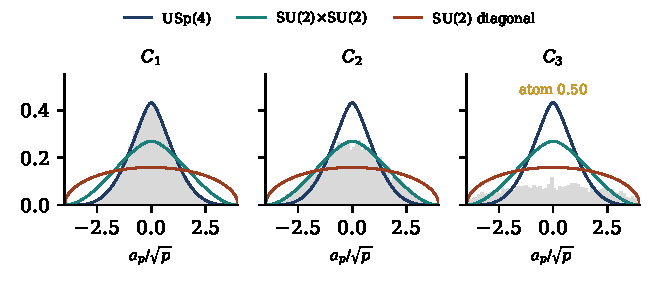
\includegraphics[width=0.92\textwidth]{figs/genus2.pdf}
\caption{Histograms of $a_p/\sqrt p$ for $C_1$, $C_2$ and $C_3$ at the good primes $p<10^5$, against the trace densities of $\USp(4)$, $\SU(2)\times\SU(2)$ and $\SU(2)$ diagonal. For $C_3$ the histogram shows the primes with $a_p\neq0$, scaled to total mass $0.50$; the atom at $0$ carries the rest.}\label{fig:12genus2}
\end{figure}

\begin{figure}[htbp]\centering
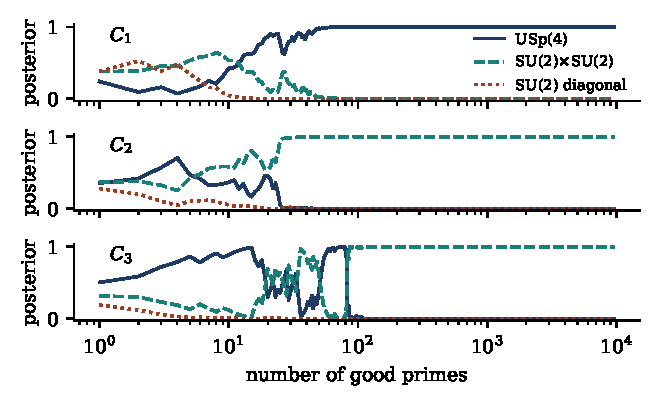
\includegraphics[width=0.78\textwidth]{figs/ch12_posterior.pdf}
\caption{Posterior probabilities of $\USp(4)$, $\SU(2)\times\SU(2)$ and $\SU(2)$ diagonal for $C_1$, $C_2$ and $C_3$ against the number of good primes (logarithmic scale), uniform prior. For $C_3$, whose group is not a candidate, the posterior settles on $\SU(2)\times\SU(2)$ after about $100$ primes.}\label{fig:12posterior}
\end{figure}

\section{Misspecification}

Berk \cite{berk1966} showed that when the true law $\mu_0$ is outside a parametric model, the posterior concentrates, under regularity conditions, on the Kullback Leibler projection, the set of parameters minimising $\mathrm{KL}(\mu_0\|P_\theta)$; see \cite{kleijnvandervaart2006} for infinite dimensional models.\index{misspecification} Theorem~\ref{thm:12consist} is the deterministic form for two candidates: the rate $\mathrm{KL}(\mu_0\|P_0)-\mathrm{KL}(\mu_0\|P_1)$ favours the candidate closer to $\mu_0$.

For $C_3$ the true law $\mu_0\approx\frac12\delta_0+\frac12\,\mathrm{law}(2x)$ has an atom and every candidate is continuous, so every divergence $\mathrm{KL}(\mu_0\|\mu_G)$ is infinite and the projection is undefined. A likelihood computed from densities scores the atom by the density value at $0$, and with $f_G$ the trace density of $G$ the posterior then concentrates on the maximiser of $\frac12\log f_G(0)+\frac12\E\log f_G(2x)$, with $x$ semicircular. The values $f_G(0)$ are $0.432$, $0.270$ and $0.159$ for $\USp(4)$, $\SU(2)\times\SU(2)$ and the diagonal group, so the atom favours the peaked $\USp(4)$ density, the continuous part favours the diagonal group, and the compromise is $\SU(2)\times\SU(2)$: predicted rates against $\USp(4)$ are $0.164$ (product) and $0.031$ (diagonal), observed $0.158$ and $0.021$, and the posterior on the product exceeds $0.99$ after $100$ primes. This is an artefact of how the atom is scored.

The honest reading for $C_3$ is \emph{none of the candidates}: a posterior near one measures fit relative to the list. The moments expose the problem at once: for every candidate at least one of them is off by dozens of standard errors (for $\SU(2)\times\SU(2)$ the second moment fits, the fourth and sixth do not). The likelihood is far less sensitive: the average log likelihood under the winner is $-1.80$ per prime, against $-1.75$ expected if the traces followed the winning law, a gap of about seven standard errors after $9590$ primes. The remedy is expansion to all $52$ groups of \cite{fkrs2012}, which forces the likelihood to carry discrete components: atoms at $a_1=0$ from disconnected groups with components on which the trace vanishes identically. With Lebesgue measure plus atoms as reference, as in Theorem~\ref{thm:12consist}, the atom alone separates $C_3$ from every connected candidate: each prime $p\equiv2\bmod3$ adds $\log(1/(2\varepsilon))$ to the log Bayes factor if the connected candidates carry a small atom $\varepsilon$ at $0$, as in the elliptic case, and the clipping level $M$ if they carry none.

\section{Nonparametric alternatives and arithmetic priors}

Distrusting the candidate list, one can put a nonparametric prior on the trace law. Dirichlet process draws \cite{ferguson1973} are discrete, so against a parametric $\mu_G$ a P\'olya tree \cite{lavine1992} or a Dirichlet process mixture is more natural; the Bayes factor of $\mu_G$ against such a prior is a test of fit of $\mu_G$ itself rather than a comparison within the list. Alternatively, a prior on moment sequences through the canonical moments of Dette and Studden \cite{dettestudden1997}, free coordinates in $(0,1)$ for the moment space of $[-4,4]$, tests whether the empirical sequence lies near some fingerprint. A roughness prior in the sense of Good and Gaskins, on densities of the eigenvalue angles that vanish on the walls of the alcove, has, formally, the Sato Tate law of a simply connected group as its mode, and for $\SU(2)$ it shrinks the empirical moments of the symmetric powers towards those of that law (Theorem~\ref{thm:lapgg}). The Dirichlet process has already appeared in Chapter~\ref{ch:pd}, not as a prior but as the limit law of the normalised Frobenius labelled factorisation of a random integer, with the Haar measure of Chebotarev's theorem as its base measure.\index{Dirichlet process}

Arithmetic should inform the prior. The Sato Tate group of an abelian surface $A$ is determined by its Galois endomorphism type, the real algebra $\mathrm{End}(A_{\overline\Q})\otimes\R$ with its Galois action \cite{fkrs2012}, which can be computed rigorously \cite{cmsv2019}; in particular, the component group of the Sato Tate group is the Galois group of the smallest field over which all endomorphisms are defined. For $C_3$ the automorphism $(x,y)\mapsto(\zeta_3x,y)$ induces an endomorphism of the Jacobian that is defined over $\Q(\sqrt{-3})$ but not over $\Q$, so the group of $C_3$ is disconnected and none of the three connected candidates can be right, a fact available before any prime is examined. Once the endomorphism type is known, Frobenius data test the Sato Tate conjecture rather than estimate the group. Across a database, group frequencies among curves of bounded conductor give an empirical Bayes prior \cite{robbins1956}, dominated by $\USp(4)$.\index{empirical Bayes}

\section{Notes}

The moment method in genus $2$ goes back to Kedlaya and Sutherland \cite{kedlayasutherland2009}; the classification \cite{fkrs2012} and the survey \cite{sutherland2019} systematise it. Equidistribution is proved for many but not all of the $52$ groups, and is open for $\USp(4)$ (Chapter~\ref{ch:03}).

The core of Theorem~\ref{thm:12consist}, that the average log likelihood ratio converges to a difference of divergences, is the argument of Wald's proof that maximum likelihood is consistent \cite{wald1949}, with equidistribution in place of the strong law of large numbers; the divergence is that of Kullback and Leibler~\cite{kullbackleibler1951}. Theorem~\ref{thm:12consist} and Corollary~\ref{thm:12elliptic} are ours; they assume equidistribution and prove nothing new about Sato Tate.

\section{Exercises}

\begin{enumerate}
\item Prove $\int_0^\pi\log\sin\theta\,d\theta=-\pi\log2$ without Fourier series, by the substitution $\theta\mapsto2\theta$ and symmetry. Deduce that the arcsine mean of $\log(4-x^2)$ is $0$.
\item Show that $\mathrm{KL}(\ST\|\mu_{\mathrm{CM}})=1$ while $\mathrm{KL}(\mu_{\mathrm{CM}}\|\ST)=\infty$, and explain why the atom $\varepsilon$ is needed. Show that both limits in Corollary~\ref{thm:12elliptic} improve as $\varepsilon$ decreases, and that the price is the jump $\log(1/(2\varepsilon))$ that each supersingular prime of a curve without complex multiplication adds to $\log B_n$. For which $\varepsilon$ is the rate without complex multiplication at most $-0.99$, and what is the smallest rate with complex multiplication on that range?
\item Using Proposition~\ref{thm:12usp4}, show that the $\USp(4)$ trace has fourth moment $3$ and that $f_{\USp(4)}(t)$ vanishes like $(4-|t|)^{4}$ as $|t|\to4$. Explain the asymmetry in Table~\ref{tab:12kl}.
\item (Probabilistic.) From Wald's identity and optional stopping derive the approximation $\E_1[N]\approx\log(1/\alpha)/\mathrm{KL}(P_1\|P_0)$. Evaluate it for $\SU(2)\times\SU(2)$ against $\USp(4)$ with $\alpha=10^{-6}$.
\item For the limiting law of $C_3$ and each of the three connected candidates $G$, compute numerically
\[
\tfrac12\log f_G(0)+\tfrac12\E\log f_G(2x),\qquad x\text{ semicircular},
\]
and verify that $\SU(2)\times\SU(2)$ wins.
\item Show that altering $(x_k)$ on a set of indices of density zero leaves every limit in Theorem~\ref{thm:12consist} unchanged.
\end{enumerate}

\section{Open computational problems}

\begin{compproblem}[The group of $y^2=x^6+x^3+1$]
Objective: identify the Sato Tate group of $C_3$ among the $52$ groups of \cite{fkrs2012} from Frobenius data; its trace moments point to $E_2$ and $J(E_1)$ in the notation of \cite{fkrs2012}, which share the law of $a_1$. Data: the normalised coefficients $(a_1,a_2)$ of the $L$ polynomial at all good primes below $2^{30}$. Route: \texttt{smalljac} or average polynomial time point counting \cite{harveysutherland2014}; moments of $a_1$ and $a_2$ up to order $12$ and the frequency of $a_1=0$ by residue class mod $3$, compared with the tables of \cite{fkrs2012} and checked against the endomorphism type \cite{cmsv2019}. Deliverable: the group, its posterior against the other group with the same law of $a_1$, and the number of primes needed to reach $1-10^{-9}$. Why it matters: it completes this chapter's misspecified example and measures what $a_2$ adds.
\end{compproblem}

\begin{compproblem}[A likelihood library, a classifier and the error exponent matrix]
Objective: build the joint densities of $(a_1,a_2)$ for all $52$ groups, atoms and lower dimensional components included, as densities against a reference measure in the sense of Theorem~\ref{thm:12consist}; compute the $52\times52$ matrix of divergences $\mathrm{KL}(\mu_G\|\mu_{G'})$ for $(a_1,a_2)$ and for $a_1$ alone (infinite where $\mu_G$ charges a set that $\mu_{G'}$ does not, and zero for $a_1$ alone when two groups share its law); and run Wald's test on every genus $2$ curve in the LMFDB \cite{lmfdb} with primes up to $10^7$. Route: Weyl integration on identity components in Sage, Monte Carlo on cosets ($10^8$ draws per group), exact arithmetic on atoms. Deliverable: the library, the divergence matrix with its near ties, a confusion matrix against the LMFDB labels, and stopping times against $\log(1/\alpha)/\mathrm{KL}$. Why it matters: the divergences are the error exponents of every test, and the near ties are the hard instances. The library and the divergence matrix are the new objects here; the run to $10^7$ is a pilot for Computational Problem~3.2, which goes to $2^{30}$, and the library must reproduce the Weyl fingerprints of Computational Problem~4.2.
\end{compproblem}

\begin{compproblem}[Genus three with an empirical Bayes prior]
Objective: extend the classifier to the $410$ groups of genus $3$ \cite{fks2021}, building on Sutherland's computations. Data: plane quartics and hyperelliptic curves of genus $3$ with discriminant below $10^7$, primes up to $2^{26}$. Route: average polynomial time point counting \cite{harveysutherland2014} and a Dirichlet prior on group frequencies estimated across the database. Deliverable: frequencies, posteriors, and curves fitted by no group. Why it matters: with $410$ candidates, shared trace laws and near ties should be far more common than in genus $2$, and the experiment measures how much of the classification Frobenius data can resolve. It builds on the genus $3$ sample of Computational Problem~3.2, adding a prior estimated across the database and a search for the curves that no group fits.
\end{compproblem}

\chapter{Open Problems}\label{ch:13}

In his 1900 address Hilbert remarked that a branch of science is alive as long as it offers an abundance of problems. Langlands' letter to Weil of 1967 and his 1970 paper \cite{langlands1970} supplied such an abundance, and more than half a century of work has settled only part of it. This chapter collects twelve problems on which the probabilistic point of view of this book has something definite to say. We do not pretend that probability will settle the central conjectures: the limits proposition (Proposition~\ref{prop:01limits}) shows that no functional of the empirical law of Frobenius traces can detect automorphy. What probability does supply is a language for quantitative refinements: rates, fluctuations, large deviations, extreme values, hitting times and sequential tests. For each problem we give the statement, its status with attributions, what probability and our computations contribute, and what would be needed. Where we do not know the right answer, the problem is posed as a question. Chapter~\ref{ch:14} collects computational versions of several of them. Chapter~\ref{ch:squarefree} poses two further problems, on the squarefree error under the Riemann hypothesis and on the signs of the P\'olya kernels of imaginary quadratic fields (Open Problems~\ref{op:sfquarter} and \ref{op:sfdensity}), Chapter~\ref{ch:beta} four on Dirichlet's $\beta$ function and the lines to the right of the centre (Open Problems~\ref{op:betacoupling} to \ref{op:betarecip}), and Chapter~\ref{ch:scholze} two on P\'olya kernels and signed Thorin measures (Open Problems~\ref{op:scholzekernel} and \ref{op:scholzelobe}). Chapter~\ref{ch:recip} poses eight problems on reciprocity (Open Problems~\ref{op:recipgln} to \ref{op:recipdrift}). Chapter~\ref{ch:hit} poses two on isogeny graphs and hitting times (Open Problems~\ref{op:hitsandpile} and \ref{op:hitgross}). Chapter~\ref{ch:flt} poses three, on the Hasse Weil bound, on patching and on Mazur's theorem (Open Problems~\ref{op:flthasse} to \ref{op:fltmazur}). Chapter~\ref{ch:lap} poses two, on the stable recovery of Frobenius traces from a window of the transported density and on penalised estimators of Thorin densities (Open Problems~\ref{op:lapwindow} and \ref{op:lapgg}). Chapter~\ref{ch:pd} poses three, on an upper bound for the rate of the Dirichlet process limit, on the signs of the Mertens deficits of fields with group $S_n$ and on an arithmetic counterpart of Bondesson's product theorem (Open Problems~\ref{op:pdrate} to \ref{op:pdproduct}). Chapter~\ref{ch:gl1} poses three, on the discrepancy of Hecke angles, on the Euler Kronecker constants of Hecke characters and on an effective Gamma shape test (Open Problems~\ref{op:gl1disc} to \ref{op:gl1cm}), and Chapter~\ref{ch:maass} four, on the Thorin representation at the centre, on a Chebotarev theorem for geodesics, on the even icosahedral representations and on the cutoff of Brownian motion on $X(N)$ (Open Problems~\ref{op:mscentre} to \ref{op:mscutoff}).

\section{Spectral problems}

\begin{problem}[Ramanujan Petersson for Maass forms]\label{op:rp}
Let $\phi$ be a Hecke Maass cusp form for $\SL_2(\Z)$ or for a congruence subgroup, with Satake parameters $\{\alpha_p,\alpha_p^{-1}\}$ at an unramified prime $p$, real Hecke eigenvalue $\lambda_\phi(p)=\alpha_p+\alpha_p^{-1}$ and Laplace eigenvalue $\lambda=\tfrac14+r^2$. Show that $|\alpha_p|=1$ for every such $p$, equivalently $|\lambda_\phi(p)|\le 2$, and that $r$ is real, which is Selberg's eigenvalue conjecture $\lambda\ge \tfrac14$.
\end{problem}

\paragraph{Status.} For holomorphic forms the analogue is Deligne's theorem \cite{deligne1974}; Maass forms have no motive and no geometric route is known.\index{Ramanujan Petersson conjecture} Selberg proved $\lambda\ge \tfrac{3}{16}$ and conjectured $\lambda\ge \tfrac14$ \cite{selberg1965}; for $\SL_2(\Z)$ itself the eigenvalue part is classical, since the cuspidal spectrum starts far above $\tfrac14$.\index{Selberg eigenvalue conjecture} The best general bounds, $|\alpha_p|\le p^{7/64}$ and $\lambda\ge \tfrac{975}{4096}$, are due to Kim and Sarnak \cite{kimsarnak2003}, from the automorphy of $\Sym^4$. Sarnak's density hypothesis \cite{sarnakxue1991}, proved in many cases, says that exceptional parameters are rare in a quantitative sense.

\paragraph{What probability and computation contribute.} By the trace formula the eigenvalues $\lambda_\phi(p)$, for $\phi$ on $\SL_2(\Z)$ ordered by Laplace eigenvalue, equidistribute with respect to the Plancherel measure $\mu_p$ \cite{sarnak1987}: the spectral measure at the root $o$ of simple random walk $S$ on the $(p+1)$ regular tree, rescaled to $[-2,2]$ (Chapter~\ref{ch:07}). Its moments $\int x^{2m}\,d\mu_p=(p+1)^{2m}p^{-m}\Prob(S_{2m}=o)$ grow like $4^m$ up to a polynomial factor. Hence if, in a family of $V$ forms, the averages of $\lambda_\phi(p)^{2m}$ match these moments up to $m\approx c\log V$, Markov's inequality bounds $\#\{\phi:|\lambda_\phi(p)|\ge2+\delta\}$ by $V(1+\delta/2)^{-2m}$ times a polynomial in $m$, that is, by $V^{1-2c\log(1+\delta/2)}$ up to such factors: the density hypothesis read as a large deviation bound for a random walk spectral measure. For the holomorphic analogue $\tau$, the primes below $10^6$ give $\max|\tau(p)/p^{11/2}|=1.99920$.

\paragraph{What would be needed.} Family averages cannot exclude a single exception. Individual bounds follow from automorphy of all $\Sym^n\phi$ by the tensor power trick \cite{langlands1970}; Newton and Thorne proved this automorphy for holomorphic newforms \cite{newtonthorne2021,newtonthorne2021b} through their Galois representations, which Maass forms in general lack.

\begin{problem}[Lang and Trotter]\label{op:lt}
Let $E/\Q$ be an elliptic curve of conductor $N_E$ without complex multiplication, let $t\in\Z$, and let $\pi_{E,t}(x)=\#\{p\le x:\ p\nmid N_E,\ a_p(E)=t\}$. Show that
\[
\pi_{E,t}(x)\ \sim\ C_{E,t}\,\pi_{1/2}(x),\qquad \pi_{1/2}(x)=\int_2^x\frac{du}{2\sqrt u\,\log u},
\]
whenever the constant $C_{E,t}$ predicted by Lang and Trotter \cite{langtrotter1976} is positive; when $C_{E,t}=0$ a congruence obstruction on the image of Galois makes the set finite.\index{Lang Trotter conjecture}
\end{problem}

\paragraph{Status.} Open for every pair $(E,t)$ with $C_{E,t}>0$. Elkies proved that every elliptic curve over $\Q$ has infinitely many supersingular primes \cite{elkies1987}, and, with Kaneko and M. R. Murty, that $\pi_{E,0}(x)=O(x^{3/4})$ \cite{elkies1991}; for every $t$, $\pi_{E,t}(x)=O(x(\log\log x)^2/(\log x)^2)$, as claimed by V. K. Murty \cite{murty1997} and proved by Thorner and Zaman \cite{thornerzaman2018}. Under the generalized Riemann hypothesis Zywina \cite{zywina2015}, improving Serre \cite{serre1981} and Murty, Murty and Saradha \cite{murtymurtysaradha1988}, proved $\pi_{E,0}(x)=O(x^{3/4}(\log x)^{-1/2})$ and $\pi_{E,t}(x)=O(x^{4/5}(\log x)^{-3/5})$. All are far above the predicted order $x^{1/2}/\log x$. On average over families the conjecture holds: Fouvry and Murty \cite{fouvrymurty1996} for $t=0$, David and Pappalardi \cite{davidpappalardi1999} for $t\ne0$.

\paragraph{What probability and computation contribute.} The conjecture is a local limit theorem with arithmetic corrections: the Sato Tate density at $0$ is $1/\pi$, the lattice spacing of $x_p$ is $1/\sqrt p$, and summing $1/(\pi\sqrt p)$ over primes gives $(2/\pi)\pi_{1/2}(x)$, which a Haar measure computation on the image of Galois in $\GL_2(\hat\Z)$ then corrects. For the curve $E_1\colon y^2=x^3+x+1$ of Chapter~\ref{ch:05} the counts of supersingular primes are $10$, $23$, $79$, $210$ at $x=10^4,\dots,10^7$, with ratios to $\pi_{1/2}(x)$ of $0.66$, $0.65$, $0.89$, $0.91$.

\paragraph{What would be needed.} Apart from the unconditional bound for $t=0$, which comes from singular moduli, the upper bounds above come from forms of the Chebotarev theorem in the division fields $\Q(E[\ell])$, whose error terms grow with the degree of the field even under the generalized Riemann hypothesis. An asymptotic requires control of a set of primes of density zero at the scale $x^{1/2}/\log x$, finer than any form of the Chebotarev theorem now available.

\begin{problem}[Optimal discrepancy and a functional limit theorem]\label{op:disc}
Let $E/\Q$ be without complex multiplication, let $p_1<p_2<\cdots$ be its primes of good reduction, $F_n$ the empirical distribution function of $x_{p_1},\dots,x_{p_n}$, $F_{\mathrm{ST}}$ that of $\ST$, and $D_n=\sup_x|F_n(x)-F_{\mathrm{ST}}(x)|$.
\begin{enumerate}[label=(\alph*)]
\item Show that $D_n=O(n^{-1/2+\delta})$ for every $\delta>0$.
\item (Question.) Let $E$ be chosen uniformly among the curves without complex multiplication of conductor at most $X$, and let $n=\lfloor X^c\rfloor$ with $c>0$ fixed. For which $c$ does $\sqrt n\,(F_n-F_{\mathrm{ST}})\circ F_{\mathrm{ST}}^{-1}$ converge in law to a Brownian bridge as $X\to\infty$, and $\sqrt n\,D_n$ to the Kolmogorov law?
\end{enumerate}
\end{problem}

\paragraph{Status.} Akiyama and Tanigawa \cite{akiyamatanigawa1999} conjectured (a) and showed that it implies the Riemann hypothesis for $L(s,E)$; Mazur \cite{mazur2008} stated the extension to every $L(s,\Sym^mE)$, under analytic hypotheses that Newton and Thorne now supply (Chapter~\ref{ch:05}). Unconditional effective forms of the Sato Tate theorem give only rates of logarithmic type \cite{thorner2021}, and the Riemann hypothesis for every $L(s,\Sym^mE)$ gives $D_n\ll n^{-1/4}$ up to logarithms (V. K. Murty \cite{murty1985}; Rouse and Thorner \cite{rousethorner2017} give an explicit form for squarefree level). For a single curve, with $n$ random on a logarithmic scale, the analogue of (b) has a negative answer under the Riemann hypothesis for $L(s,E)$, as explained below; the family version is, as far as we know, new.\index{discrepancy}\index{Brownian bridge}

\paragraph{What probability and computation contribute.} For independent draws (a) holds almost surely and (b) is Donsker's theorem. For a single curve, under the Riemann hypothesis for $L(s,E)$, the explicit formula argument of Section~\ref{sec:05disc} makes the first Chebyshev mode $n^{-1/2}\sum_{j\le n}x_{p_j}$ of order $(\log n)^{-1/2}$ in logarithmic mean square, whereas a Brownian bridge limit would make this continuous linear functional of the process standard normal; hence no randomisation of $n$ on a logarithmic scale, such as $n$ logarithmically uniform on $[N,N^2]$, produces a Brownian bridge for one curve; under the Riemann hypothesis for $L(s,\Sym^mE)$ every fixed mode $n^{-1/2}\sum_{j\le n}U_m(x_{p_j}/2)$ tends to $0$ in the same way, and Conjecture~\ref{conj:05bridge} predicts that $\sqrt n\,D_n$ itself tends to $0$ in logarithmic density. In a family one expects the primes up to $p_n$ to behave independently while $p_n$ is small compared with the conductors; a central limit theorem for the first mode is known for eigenforms of level one whose weight grows faster than every power of $n$ \cite{nagoshi2006}. The explicit formula takes over once $p_n$ exceeds the conductor of $\Sym^mE$, about $N_E^m$, and its diagonal terms suggest that the $m$th mode has variance about $\min(1,m/c)$: a transition at $c=1$, below which every mode has variance near $1$ and above which the first mode is too small for a bridge. The data of Section~\ref{sec:05disc} are consistent with so slow a decay: $\sqrt n\,D_n$ shows no drift for $E_1$, and across $200$ curves a Kolmogorov Smirnov test does not separate its law from the Kolmogorov law.

\paragraph{What would be needed.} For (a), square root cancellation in the mode sums $\sum_{j\le n}U_m(x_{p_j}/2)$ uniformly for $m$ up to about $n^{1/2}$; the Riemann hypothesis for each $L(s,\Sym^mE)$ bounds the $m$th mode sum only by $m\sqrt n$ up to logarithms, because the number of zeros of bounded height grows linearly in $m$, and this is why it yields only $n^{-1/4}$. For (b), in the regime $c<1$ a central limit theorem for the modes jointly as $m$ grows, with tightness; in the regime $c>1$ the variances of the low modes, which depend on the pair correlation of the low lying zeros of the symmetric power $L$ functions in the family.

\section{Inverse problems and symmetry}

\begin{problem}[An inverse problem for automorphy]\label{op:inverse}
(Question.) Is there a criterion, stated through quantitative properties of the twisted sums $\sum_{p\le x}x_p\chi(p)\log p$ at the square root scale (rates in the law of large numbers, mean squares on the logarithmic scale, large deviation rates), uniform over Dirichlet characters $\chi$ of growing conductor, that decides whether a sequence $(x_p)$ in $[-2,2]$ indexed by the primes is close to the normalised Hecke eigenvalues $x_p(f)=a_p(f)/p^{(k-1)/2}$ of a holomorphic newform $f$ of weight $k$ with trivial nebentypus, in the sense that $\sum_{p\le x}(x_p-x_p(f))\chi(p)\log p=o(\sqrt x)$ for every $\chi$?
\end{problem}

\paragraph{Status.} The converse theorems of Hecke \cite{hecke1936}, Weil \cite{weil1967}, Jacquet and Langlands \cite{jacquetlanglands1970} and Cogdell and Piatetski Shapiro \cite{cogdellps1994} are inverse theorems of this type, but analytic: they start from the analytic continuation and functional equations of twisted $L$ functions. Chapter~\ref{ch:recip} restates the hypotheses of Hecke's theorem as a symmetry of a P\'olya kernel built from the coefficients (Proposition~\ref{prop:recipsym}), and the holomorphy and the generalized Riemann hypothesis of a self dual Artin $L$ function as the complete monotonicity of a heat trace computed from Frobenius traces, the conductor and the gamma factor (Theorem~\ref{thm:recipcm}); these are reformulations, and Open Problems~\ref{op:recipgln} and \ref{op:reciplaw} pose related questions. Chapter~\ref{ch:lap} computes the P\'olya kernel of an Artin $L$ function by Bromwich inversion on the critical line, given that the $L$ function is entire; that the result is modular is again the content of Weil's converse theorem (Proposition~\ref{prop:lappolya}).\index{converse theorem}

\paragraph{What probability and computation contribute.} By Corollary~\ref{cor:01functional} and the remark after it, no statistic that is unchanged when the $x_p$ are altered on a set of primes of density zero, such as a limit of averages with weight $O(1/\pi(x))$ per prime, twisted or not, can decide automorphy. Rates at the square root scale cannot decide it either, which is why the question asks only for closeness: if $S$ is an infinite set of primes with $\theta_S(x)=\sum_{p\in S,\,p\le x}\log p=o(\sqrt x)$, such as the primes $p_{2^j}$, altering the $x_p(f)$ within $[-2,2]$ at every prime of $S$ changes each twisted sum by at most $4\theta_S(x)=o(\sqrt x)$ and leaves every such rate unchanged, while by Proposition~\ref{prop:01limits} the altered sequence agrees at all but finitely many primes with no such newform. Pointwise bounds do not suffice: independent variables with the Sato Tate law satisfy, almost surely, $\sum_{p\le x}x_p\chi(p)\log p\ll\sqrt x\log(qx)$ for all characters $\chi$ of conductor $q\le x$, and are almost surely close to no newform, since the newforms are countable and for each of them the untwisted sum of the differences fluctuates on the scale $\sqrt{x\log x}$. Mean squares on the logarithmic scale separate them: under the generalized Riemann hypothesis, for a newform $f$ the function $e^{-y/2}\sum_{p\le e^y}x_p(f)\chi(p)\log p$ is almost periodic in mean square, with frequencies the ordinates of the zeros of $L(s,f\otimes\chi)$, and so bounded in mean square, while for independent variables its mean square grows like $y$. Square root cancellation for every twist, even with a logarithmic loss, makes the twisted $L$ functions holomorphic and nonvanishing in $\operatorname{Re}s>\tfrac12$, but it does not give their functional equations.

\paragraph{What would be needed.} A theorem converting such rates into the hypotheses of Weil's converse theorem, not for $(x_p)$ itself, which may carry an alteration that the rates cannot see, but for a sequence reconstructed from the rates, for instance from the frequencies above; we do not know whether such a statement can be true without the root numbers.

\begin{problem}[General Sato Tate groups and symmetry types]\label{op:stgroups}
(a) For abelian varieties and motives over number fields, determine the Sato Tate group and prove equidistribution with respect to its Haar measure. (b) For natural families of $L$ functions, prove the Katz and Sarnak predictions for low lying zeros for test functions of unrestricted Fourier support.
\end{problem}

\paragraph{Status.} For elliptic curves without complex multiplication over totally real fields, (a) is the theorem of Clozel, Harris, Shepherd Barron and Taylor, completed by Barnet Lamb, Geraghty, Harris and Taylor \cite{cht2008,hsbt2010,taylor2008,blght2011}; over CM fields it was proved by Allen, Calegari, Caraiani and seven coauthors \cite{allen2023}. For abelian surfaces there are exactly $52$ groups \cite{fkrs2012}; equidistribution is known for many with extra endomorphisms \cite{johansson2017} but not for $\USp(4)$. For abelian threefolds Fit\'e, Kedlaya and Sutherland announced a classification with $410$ groups \cite{fks2021}. For (b), Katz and Sarnak \cite{katzsarnak1999,katzsarnak1999b} prove the function field analogue; over number fields only restricted support is known \cite{ils2000}, as for the $n$ level correlations of a single $L$ function \cite{rudnicksarnak1996}.\index{Sato Tate group}\index{symmetry type}

\paragraph{What probability and computation contribute.} Both parts concern pushforwards of Haar measure: in (a) to the conjugacy classes of the group, in (b) to the eigenvalue statistics of the symmetry group. In (b), restricted support means that the $n$ level densities are known only against test functions whose Fourier transforms have bounded support, which falls short of determining them, much as finitely many moments fall short of determining a law. The Weyl averages of $E_1$ and of $E_2\colon y^2=x^3-x$ in Figure~\ref{fig:04weyl} of Chapter~\ref{ch:04} match the generic and the CM law; how fast such agreement identifies the group is Open Problem~\ref{op:bayes}.

\paragraph{What would be needed.} For (a), already for a generic abelian surface, potential automorphy of the Galois representation composed with every irreducible representation of $\USp(4)$, not only the symmetric powers; for (b), a number field substitute for monodromy.

\begin{problem}[Functoriality beyond known cases]\label{op:funct}
Prove functoriality for $\GL_m\times\GL_n\to\GL_{mn}$ in general, and for $\Sym^n:\GL_2\to\GL_{n+1}$ for Maass forms and all $n$.
\end{problem}

\paragraph{Status.} Known cases include $\Sym^2$ \cite{gelbartjacquet1978}, $\GL_2\times\GL_2$ \cite{ramakrishnan2000}, $\GL_2\times\GL_3$ and $\Sym^3$ \cite{kimshahidi2002}, $\Sym^4$ (Kim \cite{kimsarnak2003}), all symmetric powers for holomorphic newforms \cite{newtonthorne2021,newtonthorne2021b}, and the transfers from quasi split classical groups to $\GL_N$ \cite{arthur2013}; see \cite{arthur2003,gelbart1984}.\index{functoriality}

\paragraph{What probability and computation contribute.} Functoriality has consequences that Frobenius data can test. For an elliptic curve without complex multiplication, automorphy and cuspidality of every symmetric power give the Sato Tate law, and the even moments of $x_p$ for $E_1$ over the good primes below $10^7$ agree with the Catalan numbers $1,2,5,14,42,132$ to a relative error below $6\times10^{-4}$ (Chapter~\ref{ch:05}). For cuspidal $\pi_1,\pi_2$ on $\GL_2$, cuspidality of $\pi_1\boxtimes\pi_2$ on $\GL_4$ gives
\[
\sum_{p\le x}\frac{|\tr A_p(\pi_1)|^2\,|\tr A_p(\pi_2)|^2}{p}\sim\log\log x,
\]
which for two elliptic curves without complex multiplication that are not twists of each other is the moment identity $\int\!\!\int x^2y^2\,d\ST(x)\,d\ST(y)=1$.

\paragraph{What would be needed.} The known cases came from the Langlands Shahidi method and converse theorems (Gelbart and Jacquet, Ramakrishnan, Kim and Shahidi, Kim), from the trace formula (Arthur) and from automorphy lifting (Newton and Thorne). By the limits proposition the checks above are functionals of empirical laws and cannot replace such methods.

\section{Graphs}

\begin{problem}[Ramanujan graphs of all degrees]\label{op:graphs}
Give a deterministic algorithm that, for each $d\ge 3$ and all large $n$ with $nd$ even, constructs in time polynomial in $n$ a nonbipartite $d$ regular graph on $n$ vertices whose nontrivial eigenvalues satisfy $|\lambda|\le 2\sqrt{d-1}$.
\end{problem}

\paragraph{Status.} The arithmetic constructions of Chapter~\ref{ch:08} (Lubotzky, Phillips and Sarnak; Margulis; Morgenstern; Pizer) give special sequences of $n$ only; the probabilistic results of that chapter give nearly Ramanujan graphs (Friedman, Bordenave), bipartite Ramanujan multigraphs of every degree and every even number of vertices (Marcus, Spielman and Srivastava) and, since about $69$ percent of random $d$ regular graphs are Ramanujan (Huang, McKenzie and Yau~\cite{hmy2024}, a 2024 preprint), existence for all large $n$ and a randomised polynomial time construction (sample a graph and test its spectrum). Deterministic polynomial time constructions reach $|\lambda|\le2\sqrt{d-1}+\varepsilon$ for every $d\ge3$ and $\varepsilon>0$ (Mohanty, O'Donnell and Paredes \cite{mop2022}), on exactly $n$ vertices for all large $n$ with $nd$ even (Alon \cite{alon2021}); the problem asks for $\varepsilon=0$, which, as far as we know, no deterministic construction achieves for nonbipartite graphs of all large sizes.\index{Ramanujan graph}

\paragraph{What probability and computation contribute.} The existence results beyond the arithmetic constructions are probabilistic: the trace method of Friedman and Bordenave, the interlacing polynomials of Marcus, Spielman and Srivastava, and the edge universality around the Kesten McKay law of Huang, McKenzie and Yau.

\paragraph{What would be needed.} Derandomisation of the random constructions, which Cohen \cite{cohen2016} achieved for the bipartite construction of Marcus, Spielman and Srivastava, or an arithmetic source of graphs of every degree: the arithmetic constructions above come from groups acting on the tree of $\PGL_2$ over a local field, whose degree is always a prime power plus one.

\section{Thorin measures and extreme values}

\begin{problem}[Hilbert's eighth problem for $\GL_2$ in Thorin form]\label{op:thorin}
Let $\Lambda(s,\Delta)=(2\pi)^{-s}\Gamma(s)L(s,\Delta)$, write its zeros as $6\pm i\gamma_k$ with $\operatorname{Re}\gamma_k>0$, and let $k_\Delta(x)=\sum_k e^{-\gamma_k^2x}$ for $x>0$. Prove by a probabilistic argument that $k_\Delta$ is completely monotone on $(0,\infty)$.
\end{problem}

\paragraph{Status.} Integrating termwise, $\sum_k(\gamma_k^2+s)^{-1}=\int_0^\infty e^{-sx}k_\Delta(x)\,dx$ for $s>0$, and by the Hadamard product the left side is $(d/ds)\log\Lambda(6+\sqrt s,\Delta)$. By Bernstein's theorem and the equivalence with generalized gamma convolutions in Chapter~\ref{ch:10} (Theorem~\ref{thm:ch10ggc}) the problem is equivalent to the Riemann hypothesis for $\Delta$, hence open. The parallel statement for $\xi$ is Polson's reformulation of Hilbert's eighth problem \cite{polson2017}, building on Biane, Pitman and Yor \cite{bpy2001}; the theory of generalized gamma convolutions is due to Thorin \cite{thorin1977} and Bondesson \cite{bondesson1992}.\index{Thorin measure}\index{complete monotonicity}

\paragraph{What probability and computation contribute.} A probabilistic proof would exhibit the law with Laplace transform $\Lambda(6)/\Lambda(6+\sqrt s)$, whose Lévy density is $x^{-1}k_\Delta(x)$, as a generalized gamma convolution built without the zeros, for instance from hitting or occupation times of a diffusion, as Bessel processes produce the laws of Biane, Pitman and Yor. Equivalently, the characteristic function of the Pólya variable $W$ must have only real zeros, which is Pólya's question \cite{polya1926}, with the de Bruijn Newman heat flow \cite{debruijn1950,newman1976,rodgerstao2020} as a natural deformation. The product over the $404$ zeros up to height $400$, with a tail correction, reproduces $\Lambda(6)/\Lambda(6+\sqrt s)$ for $s\le400$ to about four significant digits (relative error at most $1.9\times10^{-4}$), and $\operatorname{Var}W=0.112352$ against $0.112348$ from the zeros with the tail correction (Chapter~\ref{ch:10}). Chapter~\ref{ch:scholze} computes a smoothed signed version of this Thorin measure by Stieltjes inversion to height $30$.

\paragraph{What would be needed.} A positive measure $\tau$ on $(0,\infty)$ with $k_\Delta(x)=\int e^{-tx}\,\tau(dt)$, the Thorin measure of the problem, constructed without reference to the zeros, for example from an occupation or hitting time law; such a construction would prove the Riemann hypothesis for $\Delta$. Positivity of $k_\Delta$ alone, which is infinite divisibility, would not suffice. Open Problem~\ref{op:recipfejer} asks whether a positive summation of the prime side of the explicit formula can play the part that Fej\'er's kernel plays for the circle (Proposition~\ref{prop:recipfejer}).

\begin{problem}[The extreme value representation]\label{op:ev}
Let $M^*$ be the maximum of $24$ independent copies of $M=\max_{n\ge1}E_n/(2\pi n)$, with $E_n$ independent standard exponential variables, so that $L(s,\Delta)=\E\,Q(s,2\pi M^*)$ with $Q(s,c)=\Gamma(s,c)/\Gamma(s)$ (Chapter~\ref{ch:11}).
\begin{enumerate}[label=(\alph*)]
\item (Question.) Can properties of the law of $M^*$, such as the self similarity $F(y)=y^{-12}e^{2\pi(y-1/y)}F(1/y)$ of its distribution function given by modularity, be used to locate or count the zeros of $L(s,\Delta)$?
\item (Question.) For which newforms $f$ is there a random variable $M_f$, the maximum of countably many independent variables with distribution functions of the form $(1-e^{-cy})^{\kappa}$ with $c,\kappa>0$, such that $f(iy)=e^{-2\pi y}\Prob(M_f\le y)$ for all $y>0$?
\end{enumerate}
\end{problem}

\paragraph{Status.} The representation is proved in Chapter~\ref{ch:11} for $\Delta$ and for every eta product $\prod_m\eta(m\tau)^{r_m}$ with $r_m\ge0$ and $\sum_m m\,r_m=24$, among them the multiplicative eta products of Dummit, Kisilevsky and McKay \cite{dkm1985} (Theorems~\ref{thm:ch11main} and \ref{thm:ch11general}), so (b) has a positive answer for those of them that are newforms. Part (a) asks for a route to Conjecture~\ref{conj:ch11rh}. As far as we know, both questions are new.\index{extreme value representation}

\paragraph{What probability and computation contribute.} By Corollaries~\ref{cor:ch11bounds} and~\ref{cor:ch11monotone}, $L(s,\Delta)$ lies in $(0,1)$ and increases on $s>0$. On the critical line the functional equation gives
\[
\Lambda(6+it,\Delta)=2\,\E\int_{\max(1,M^*)}^\infty e^{-2\pi y}y^5\cos(t\log y)\,dy,
\]
so (a) asks for the sign changes in $t$ of an explicit expectation, the analogue of Hardy's function. By uniqueness of Laplace transforms, (b) holds exactly when the exponents $\kappa_m$ in the formal product $q^{-1}f=\prod_{m\ge1}(1-q^m)^{\kappa_m}$ are all nonnegative and the product converges for $0<q<1$; for nonnegative $\kappa_m$ this convergence is equivalent to $f$ having no zeros in the upper half plane. Chapter~\ref{ch:11} checks the representation to $16$ digits and by Monte Carlo.

\paragraph{What would be needed.} For (a), a property of the specific law of $M^*$ that fails for nearby laws, since expectations built from nearby laws need not have their zeros on a line. For (b), a description of the newforms with no zeros in the upper half plane, whose divisors are supported on the cusps, together with the signs of their exponents $\kappa_m$; eta quotients are the basic examples, Borcherds products are a natural framework for the exponents, and Martin's classification of the multiplicative eta quotients \cite{martin1996} is the place to start.

\section{Hitting times, inference and bias}

\begin{problem}[Kemeny constants of isogeny graphs at finite level]\label{op:kemeny}
For primes $N\equiv1\bmod 12$ let $K_N$ be the Kemeny constant of simple random walk on the supersingular $2$ isogeny graph in characteristic $N$, which is $3$ regular on $h=(N-1)/12$ vertices, so that $K_N/h\to2$ (Theorem~\ref{thm:08kemeny}). (Question.) Does the empirical distribution of $K_N-2h$ over the primes $N\le Y$ in this class converge as $Y\to\infty$, and is $K_N-2h$ bounded?
\end{problem}

\paragraph{Status.} The first order law is Theorem~\ref{thm:08kemeny} of Chapter~\ref{ch:08}, proved from Serre's vertical equidistribution \cite{serre1997} and the Brandt matrix identification \cite{pizer1990}. The second order term has not been studied as far as we know; hitting times matter for isogeny based hash functions \cite{cgl2009}.\index{Kemeny constant}

\paragraph{What probability and computation contribute.} By Theorem~\ref{thm:A:kemeny} and Remark~\ref{rem:08exact},
\[
K_N=\sum_{j\ge2}\frac{1}{1-\lambda_j/3}=\frac32\sum_{m\ge0}2^{-m}\tr\bigl(T_{2^m}\mid S_2(\Gamma_0(N))\bigr),
\]
where $\lambda_2,\dots,\lambda_h$ are the eigenvalues of $T_2$ on $S_2(\Gamma_0(N))$. The Eichler Selberg trace formula writes $\tr T_{2^m}$ as $(N+1)/12$ for even $m$, plus terms independent of $N$, minus half the sum of the Hurwitz class numbers $H(2^{m+2}-t^2)$ weighted by $1+\bigl(\tfrac DN\bigr)$, $D=t^2-2^{m+2}$. The main terms add up to $(N+1)/6=2h+\tfrac13$, so that, formally, $K_N-2h=c_0+\sum_Dw_D\bigl(\tfrac DN\bigr)$ with explicit constants $c_0$ and $w_D\le0$, the sum running over negative fundamental discriminants $D\ne-3,-4$. On this progression $\bigl(\tfrac DN\bigr)$ is the product of the signs $\varepsilon_q=\bigl(\tfrac qN\bigr)$ over the primes $q\ne3$ that divide $D$ to an odd power, and by Dirichlet's theorem, for each finite set of primes $q$, the signs $\varepsilon_q$ are asymptotically independent and fair as $N$ varies. This suggests that $K_N-2h$ converges in law to the random multiplicative series obtained by taking the $\varepsilon_q$ independent. Size estimates suggest that the weights are square summable, so that this series converges in mean square, but not absolutely summable, so that $K_N-2h$ may be unbounded, with large negative values at levels where $\varepsilon_q=1$ for many small primes $q$. Over the $207$ levels $1000<N<8000$ computed for this book, $K_N-2h$ lies between $-17.7$ and $6.9$ with mean $-7.0$; its mean is $-11.0$ when $\bigl(\tfrac{-7}{N}\bigr)=1$ and $-3.3$ when $\bigl(\tfrac{-7}{N}\bigr)=-1$ (Chapter~\ref{ch:08}).

\paragraph{What would be needed.} Control of the trace formula with weights $2^{-m}$ up to $m$ of order $2\log_2N$, beyond which the Ramanujan bound controls the tail; cancellation in the class number sums for discriminants larger than $N$, where the symbols $\bigl(\tfrac DN\bigr)$ are periodic in $D$ rather than independent; and joint equidistribution of the signs $\varepsilon_q$ for $q$ up to a power of $N$, a large sieve statement.

\begin{problem}[Bayesian identification of Sato Tate groups]\label{op:bayes}
(a) Extend Theorem~\ref{thm:12consist} to the $52$ Sato Tate groups of abelian surfaces, whose laws of the normalised coefficients $(a_1,a_2)$ can have atoms and components on lower dimensional sets, and to motives of higher rank. (b) Make it effective: bound the number of primes after which the log Bayes factor favours the true group against every other candidate, polynomially in the logarithm of the conductor and without assuming the Riemann hypothesis.
\end{problem}

\paragraph{Status.} Theorem~\ref{thm:12consist} gives the double limit $\lim_{M\to\infty}\lim_{n\to\infty}n^{-1}\log B_n^M=\mathrm{KL}(\mu_0\|P_0)-\mathrm{KL}(\mu_0\|P_1)$ for the log Bayes factor $\log B_n^M$ of $P_1$ against $P_0$ clipped at level $M$, when $P_0$, $P_1$ and the limit law $\mu_0$ of the data have densities on a compact set with respect to Lebesgue measure plus counting measure on a fixed finite set $D$ and the data are equidistributed for $\mu_0$ relative to $D$, under the further conditions stated there; Chapter~\ref{ch:12} applies it to elliptic curves and to three candidates in genus $2$. The classification \cite{fkrs2012} matches curves to groups by moments, not by sequential tests; several of the $52$ groups share the law of $a_1$, so the pair $(a_1,a_2)$ is needed. For independent observations Wald's test \cite{wald1947} is optimal for simple hypotheses \cite{waldwolfowitz1948}, with error exponents given by the divergences. For elliptic curves, effective forms of the Sato Tate theorem \cite{rousethorner2017,thorner2021} yield bounds of the kind asked in (b), polynomial in $\log N_E$ under the Riemann hypothesis for the symmetric power $L$ functions and much weaker unconditionally.\index{sequential probability ratio test}\index{Kullback Leibler divergence}

\paragraph{What probability and computation contribute.} With $\mu_0=P_0=\mu_G$ for the true group $G$ and $P_1=\mu_{G'}$ for a candidate $G'$, the double limit is $-d_{GG'}$ with $d_{GG'}=\mathrm{KL}(\mu_G\|\mu_{G'})$, so a sequential test with threshold $\log(1/\beta)$ stops after about $\log(1/\beta)/d_{GG'}$ primes. When $\mu_G$ charges a set that $\mu_{G'}$ does not, the divergence is infinite, and the small atoms and clipping of Chapter~\ref{ch:12} make it large and finite; the near ties, which set the error exponents, come from groups that differ only on components of small mass. The $52\times52$ divergence matrix is part of Computational Problem 29.2.

\paragraph{What would be needed.} For (a), reference measures adapted to the lower dimensional components, so that the clipping argument still applies; equidistribution for the true group, which is open for $\USp(4)$; and, in higher rank, the classification of the groups. For (b), unconditional effective equidistribution with power rates, which would also bear on Open Problem~\ref{op:disc}.

\begin{problem}[The rank bias]\label{op:rankbias}
Let $E/\Q$ have conductor $N_E$ and analytic rank $r_E$, let $S_E(x)=\sum_{p\le x,\,p\nmid N_E}a_p\log p/p$, and assume the Riemann hypothesis for $L(s,E)$. Then $S_E(x)-(\tfrac12-r_E)\log x$, with $\log x$ uniform on $[0,Y]$ and $Y\to\infty$, converges in law to a distribution $\mu_E$ with mean $C_E$; let $Z_E$ have the law $\mu_E$ shifted to mean zero. (Question.) As $E$ runs through the curves of conductor at most $X$ and analytic rank $r\in\{0,1\}$, does the law of $Z_E/\log N_E$ converge as $X\to\infty$, and is the limit the one predicted by the low lying zeros of the corresponding orthogonal family?
\end{problem}

\paragraph{Status.} Under the Riemann hypothesis for $L(s,E)$ the explicit formula and the method of Rubinstein and Sarnak \cite{rubinsteinsarnak1994} give the existence of $\mu_E$, and identify it as the law of $C_E-\sum_{\gamma>0}2\sin(\theta_\gamma)/\gamma$, with independent uniform phases $\theta_\gamma$, when the positive ordinates $\gamma$ of the noncentral zeros are linearly independent over $\Q$; Sarnak's letter \cite{sarnak2007} explains such biases through the explicit formula. The link between the rank and partial Euler products goes back to Goldfeld \cite{goldfeld1982} and Kuo and Murty \cite{kuomurty2005}; see Mazur \cite{mazur2008}. The family question is, as far as we know, open.\index{rank bias}\index{Chebyshev bias}

\paragraph{What probability and computation contribute.} The explicit formula gives $S_E(x)-(\tfrac12-r_E)\log x=C_E-\sum_{\gamma>0}2\sin(\gamma\log x)/\gamma+o(1)$ in logarithmic mean square: the prime squares produce the $\tfrac12$, the central zero of order $r_E$ the $-r_E$, and the other zeros an almost periodic oscillation (Chapter~\ref{ch:05}). Under linear independence $Z_E$ has variance $V_E=2\sum_{\gamma>0}\gamma^{-2}$, the same form as $\operatorname{Var}W$ in Open Problem~\ref{op:thorin}. For the four curves of Chapter~\ref{ch:05}, the central Taylor coefficients computed in Chapter~\ref{ch:10b} give $V_E=0.255$, $0.379$, $0.814$ and $1.452$ for 11a1, 37a1, 389a1 and 5077a1, increasing as the lowest noncentral zero descends from $6.36$ to $2.05$. The fitted slopes $0.46$, $-0.59$, $-1.43$, $-2.51$ against $0.5$, $-0.5$, $-1.5$, $-2.5$ (Chapter~\ref{ch:05}) are consistent with oscillations of standard deviation $\sqrt{V_E}$, between $0.5$ and $1.2$, over the range $6.9\le\log x\le16.1$. Since the lowest zeros of a curve of large conductor lie at heights of order $1/\log N_E$, $V_E$ is typically of order $(\log N_E)^2$, which explains the normalisation. If the normalised ordinates $t_j=\gamma_j\log N_E/(2\pi)$ follow the Katz Sarnak limit, the even orthogonal one for $r=0$ and the odd one with its central zero removed for $r=1$, then $Z_E/\log N_E$ should converge in law to $-\pi^{-1}\sum_j\sin(\theta_j)/t_j$, with $(t_j)$ the points of that limit and $\theta_j$ independent and uniform. For $r=0$ this limit has infinite variance, because the even orthogonal ensemble does not repel the lowest zero from the central point; for $r=1$ the repulsion makes the variance finite. The slope test at high rank is Computational Problem 5.3.

\paragraph{What would be needed.} Each $\mu_E$ needs the Riemann hypothesis for $L(s,E)$. For the family law, $V_E$ is dominated by the lowest zeros, so one needs the distribution of the lowest zero itself, which the restricted support results for the one level density \cite{ils2000} do not determine (Open Problem~\ref{op:stgroups}).

\section{Notes}

The conjectures behind Open Problems~\ref{op:inverse} and \ref{op:funct} go back to Langlands' paper \cite{langlands1970}; Arthur \cite{arthur2003} and Gelbart \cite{gelbart1984} are standard overviews. Sarnak's density hypothesis and vertical Plancherel law \cite{sarnak1987,sarnakxue1991} are the model for the probabilistic reading of Open Problem~\ref{op:rp}. Lang and Trotter \cite{langtrotter1976} derived their constant from a probabilistic model of Frobenius in the image of Galois, the model behind Open Problem~\ref{op:lt}. Mazur's essay \cite{mazur2008} is the source of the error term perspective behind Open Problems~\ref{op:disc} and \ref{op:rankbias}; in both, the explicit formula makes the arithmetic sums smaller and more structured than independent ones, the theme of the analysis of Chebyshev's bias by Rubinstein and Sarnak \cite{rubinsteinsarnak1994} and of Sarnak's letter \cite{sarnak2007}. The Thorin and extreme value problems are specific to this book.

\section{Open computational problems}

The full programme is in Chapter~\ref{ch:14}; the two problems below belong to this chapter.

\begin{compproblem}[Discrepancy at scale]\label{cp:13disc}
Objective: test the transition at $c=1$ suggested in Open Problem~\ref{op:disc}(b), and the slow decay predicted for single curves. It extends Computational Problem~\ref{cp:05bridge}, which runs $E_1$ and a family to a fixed prime bound, by tying the number of primes to the conductor, $n=\lfloor X^c\rfloor$. Scale: for $E_1$ and $10$ further curves without complex multiplication, all primes below $10^{10}$; for the family, $10^3$ curves with conductor in $[X,2X]$ from the LMFDB \cite{lmfdb} for $X=10^3$ and $10^4$, with $n=\lfloor X^c\rfloor$ for $c=\tfrac12,1,\tfrac32,2$, so at most $10^8$ primes per curve. Route: average polynomial time point counting \cite{harvey2014,harveysutherland2014}, or PARI/GP \texttt{ellap} in parallel. Deliverables: for each $X$ and $c$, the variances across the family of the modes $n^{-1/2}\sum_{j\le n}U_m(x_{p_j}/2)$ for $m\le20$, compared with $\min(1,m/c)$, and the law of $\sqrt n\,D_n$ against the Kolmogorov law with a Kolmogorov Smirnov statistic; for the single curves, the paths of $\sqrt n\,D_n$ and of the modes for $m\le200$ in $\log n$. Why it matters: the $200$ curves of Chapter~\ref{ch:05} have discriminants below $10^7$ in absolute value and use the primes below $10^6$, so $c$ is of order $1$ for them, and their standard deviation $0.219$ against $0.2603$ is consistent with a mild deficit there; varying $c$ separates the two regimes, and a deficit for $c>1$ would indicate that the explicit formula, not independence, governs the fluctuations.
\end{compproblem}

\begin{compproblem}[Second order Kemeny constants]\label{cp:13kemeny}
Objective: test the random series model of Open Problem~\ref{op:kemeny}, which Computational Problem~\ref{cp:08second} approaches through a regression on the symbols for small discriminants, whereas here the full predicted series is tested. Data: the values of $K_N-2h$ for the $19564$ primes $N\equiv1\bmod12$ below $10^6$ ($h$ up to $83330$) produced in Computational Problem~\ref{cp:08second}. Route: compute the weights $w_D$ for $|D|\le10^6$ from the trace formula, as $-\tfrac34$ times the sum of $2^{-m}H(2^{m+2}-t^2)$ over the pairs $(m,t)$ for which $t^2-2^{m+2}$ is $D$ times a square, with PARI/GP \texttt{qfbhclassno}; compare $K_N-2h$ with $c_0+\sum_Dw_D\bigl(\tfrac DN\bigr)$; and simulate the random multiplicative series with independent signs $\varepsilon_q$. Deliverables: the residuals of the prediction, the empirical law of $K_N-2h$ against the simulated law (quantile plot and Kolmogorov Smirnov statistic), and the levels with the most extreme values together with their signs $\varepsilon_q$ for $q\le100$. Why it matters: agreement would support reducing Open Problem~\ref{op:kemeny} to the joint equidistribution of Legendre symbols, and the extreme levels test whether $K_N-2h$ is bounded.
\end{compproblem}

\chapter{A Computational Programme}\label{ch:14}

Chapters~\ref{ch:01} to \ref{ch:13} of this book pose computational problems that we have deliberately left open. They are not exercises. Each one asks for a computation at a scale beyond what we carried out for the book, and each was chosen because its answer would sharpen a theorem, test a conjecture, or calibrate a heuristic that appears in the text. This chapter collects them into a single programme, organises them into workstreams, and sets out the standards we propose for carrying them out. The programme is the agenda of the second author's computational work over the coming years, and we hope that readers will take up parts of it.

\section{Principles}

The computations in this book are experiments on deterministic objects. A sequence of Frobenius traces is not a sample from a distribution; it is a fixed arithmetic sequence that, by theorem or by conjecture, behaves in the limit like one. This has consequences for how results should be reported.

\begin{enumerate}
\item Certified where possible. Point counts, Hecke matrices, isogeny graphs and $L$ function zeros can be computed exactly or with rigorous error bounds. A claim such as ``every nontrivial Ihara pole lies on the circle'' should come with the arithmetic that certifies it, not only a floating point check.
\item Statistical where necessary. When a conjecture predicts a limiting law or constant (a Brownian bridge, a Kolmogorov distribution, a Lang and Trotter constant), the test statistic, the null law and the reference population must be stated in advance. Cross sectional comparisons across many curves, as in Chapter~\ref{ch:05}, are often more informative than a single long sequence, because they turn one deterministic path into many approximately independent ones.
\item Scaled with care. Many statistics converge slowly. The scaled discrepancy $\sqrt n\,D_n$ and the rank bias are predicted to approach their limits at logarithmic rates (Chapter~\ref{ch:05}), and the Lang and Trotter counts of that chapter, which grow like $\sqrt x/\log x$ and number at most a few hundred below $10^7$, have a relative Poisson error of order $x^{-1/4}$ up to logarithmic factors. In both cases a factor of ten in the range of primes buys little. The programme favours breadth (more curves, more levels, more forms) over depth whenever the conjectured limit is a law across families.
\item Reproducible. Every table should be regenerable from a script and a seed. Appendix~\ref{app:B} prints the core routines and lists the scripts and stored results behind the numbers of this book, together with an archive of the scripts in a layout with relative paths, but several of them still read files from the wrong folder, so making every table regenerable from a single command comes before scaling the computations up.
\end{enumerate}

\section{Workstreams}

We group the problems into six workstreams. Problem N.M denotes Computational Problem N.M, the Mth computational problem of Chapter N (Problem 5.2 is the second computational problem of Chapter~\ref{ch:05}).

\subsection{Workstream I: Frobenius data at scale}

This workstream builds the basic data: traces of Frobenius for elliptic curves, genus two Jacobians and modular forms, at scales well beyond those of this book. The engine is a point counting pipeline (Problem 5.4), using baby step giant step and the average polynomial time methods of Harvey \cite{harvey2014} and of Harvey and Sutherland \cite{harveysutherland2014} for elliptic and hyperelliptic curves, and GPU kernels for the embarrassingly parallel part. On this foundation sit the Sato Tate atlas (Problem 1.1), the Weyl averages and fingerprints (Problems 4.1 and 4.2), joint laws of pairs and twists (Problems 3.3 and 4.3), the Brownian bridge test (Problems 5.1 and 31.1), the Lang and Trotter constants (Problem 5.2), Koblitz's conjecture on the primes at which the number of points is prime, whose local densities are the Eisenstein shapes of Chapter~\ref{ch:flt} (Problem 22.2), the rank bias at high rank (Problem 5.3), the Chebotarev races (Problem 3.1), Gamma process tests of Chebotarev laws, with their Euler Kronecker drifts, and of joint Sato Tate laws (Problem 20.3), Gamma shape estimates for symmetric powers and $\GL_3$ motives (Problem 20.4, a Dirichlet density counterpart of Problems 4.1 and 4.2), the three colourings of the prime factors of uniform random integers by Frobenius class, with the proportions of integers that avoid a class (Problem 24.1), the Mertens constants of the fields of $x^n-x-1$, whose group is $S_n$ (Problem 24.2), and tables of $\tau(p)$ (Problem 2.1). The impostor detection problem (Problem 1.2) is the statistical counterpart of Proposition~\ref{prop:01limits}.

\subsection{Workstream II: families, symmetry and random matrices}

The second workstream concerns families of $L$ functions. Its problems are the one level density for quadratic twists of 11a (Problem 6.1), moments of quadratic $L$ functions against the Keating and Snaith predictions (Problem 6.2), nearest neighbour spacings for the zeros of $L(s,\Delta)$ at heights from $10^8$ on (Problem 6.3, which continues Problem 12.3), Hecke eigenvalue tables for newforms of level up to $10^4$ and even weight up to $12$ (Problem 2.2), near coincidences of newforms (Problem 1.3), the congruences between newforms of level $M$ and newforms of level dividing $Mq$, new at $q$, predicted by Ribet's level raising condition, read as vanishing discrepancy Thorin masses (Problem 22.3), and the use of the functional equation defect as a test statistic (Problem 2.3), extended to the twisted P\'olya kernels of Weil's converse theorem and to Artin representations (Problem 20.2). The computational core is tables of Hecke eigenvalues and fast evaluation of $L$ functions and their zeros across large families, for which the LMFDB \cite{lmfdb} and the rigorous methods of Booker and Platt are the natural references.

\subsection{Workstream III: buildings, graphs and hitting times}

The third workstream extends Chapters~\ref{ch:07} and \ref{ch:08} and the first section of Chapter~\ref{ch:hit}. It asks for the rate of vertical convergence of Hecke spectra to the Plancherel measures (Problem 9.1), quotients of a regular tree by congruence and by random noncongruence subgroups of a Lubotzky Phillips Sarnak lattice (Problem 9.2), Plancherel statistics for $\GL_3$ through Hecke operators on quotients of the building of $\PGL_3(\Q_2)$ by lattices from definite unitary groups in three variables (Problem 9.3), the second order term of the Kemeny constant (Problems 10.1 and 31.2), the laws of the critical groups of isogeny graphs at fixed degree against the Haar model of Munier and Shnidman and the Cohen Lenstra law (Problem 21.1), hitting times between supersingular curves, which govern the cost of naive path search in isogeny cryptography, for $N$ up to $10^7$ (Problem 10.2), other degrees and ordinary isogeny volcanoes (Problem 10.3), and Ihara zeta functions of random lifts (Problem 10.4). Here exact linear algebra on sparse graphs (isogeny graphs with $N\le10^5$, so up to about $8300$ vertices, and building quotients with up to $10^5$ vertices), together with Monte Carlo walks on graphs with up to $8\times10^5$ vertices, is the main tool.

\subsection{Workstream IV: \texorpdfstring{$L$}{L} functions as laws}

The fourth workstream concerns the probabilistic representations of Part IV. It includes the value distribution of $\log L(\sigma+it,\Delta)$ against its two random Euler product models (Problem 11.1), large deviation rate functions (Problem 11.2), universality (Problem 11.3), the Thorin measure of $\Delta$ to height $10^5$ (Problem 13.1), the de Bruijn Newman constant of $\Delta$ (Problem 13.2), complete monotonicity across weights and levels (Problem 13.3), the degenerate Thorin atom for curves of rank two (Problem 13.4), tables of the extreme value laws $M_f$ for all multiplicative eta products (Problem 28.1), variance reduction and zero location by simulation (Problem 28.2), and the extension to eigenforms that are not eta products (Problem 28.3). The Thorin framework of Chapters~\ref{ch:10b} and \ref{ch:10c} adds its own problems: certified Thorin Hankel determinants computed from central derivatives (Problem 14.1), the Herglotz test (Problem 14.2), collision times of the Thorin atoms of $\Delta$ (Problem 14.3), a regularised Thorin computation for a Selberg zeta function (Problem 14.4), comb statistics against the zeros of $L(s,\Delta)$ (Problem 15.1), large deviations of passage times on finite isogeny graphs against the tree formula (Problem 15.2), local parabolic tests of the Ramanujan conjecture for Maass forms (Problem 15.3), and Thorin combs of curves of genus three and four (Problem 15.4). Chapter~\ref{ch:10d} adds four more: a certified Patie test with Bernstein gamma interpolation (Problem 16.1), transported Thorin densities at basepoints inside the critical strip (Problem 16.2), first passage tables and large deviations for Euler subordinators (Problem 16.3), and van Dantzig and P\'olya frequency tests for the partner variables of $L$ functions (Problem 16.4). Chapter~\ref{ch:squarefree} asks for the squarefree error beyond $10^{18}$ (Problem 17.1), the oscillations of the counts of squarefree ideals of $\Q(i)$ and $\Q(\sqrt{-3})$ (Problem 17.2), and the signs of the P\'olya kernels of imaginary and of real quadratic fields (Problems 17.3 and 17.4). Chapter~\ref{ch:beta} asks whether, for the real characters of conductor up to $10^3$, $\operatorname{Re}\Lambda'/\Lambda$ is smallest on the real axis along the lines to the right of the centre (Problem 18.1), carries its computations to the Hecke characters of the Gaussian field (Problem 18.2), asks for the response of its criteria to synthetic off line zeros (Problem 18.3), and adds $L(s,\chi_{-4})$ to Problem 16.2. Chapter~\ref{ch:scholze} asks for the signs of P\'olya kernels of degree up to four (Problem 19.1), zero counts by the argument principle in ball arithmetic (Problem 19.2) and the window leakage of signed Thorin densities (Problem 19.3). Chapter~\ref{ch:recip} adds the Galois heat trace of an icosahedral Artin representation with trivial determinant, hence self dual and even (Problem 20.1), where a certified violation of complete monotonicity would disprove Artin's conjecture or the generalized Riemann hypothesis for it, although finitely many such inequalities are not known to confirm them, even to a finite height; it needs the complete monotonicity pipeline of Problem 13.3 and the ball arithmetic of Problem 14.1. Chapter~\ref{ch:hit} adds the explosion cumulants of the same representation, the integrals of its heat trace against $1$ and $x$, computed from its Frobenius classes, conductor and gamma factor (Problem 21.2): on the range of $x$ that the primes control they are compared with the zeros, and in full with the power sums $\sum\gamma^{-2}$ and $\sum\gamma^{-4}$ that the route of Problem 14.1 computes from central derivatives. It also asks which real odd characters of conductor below $10^6$ have a positive signed exit density, which excludes a real zero of their $L$ function (Problem 21.3). Chapter~\ref{ch:flt} asks for the integrals of the heat trace against $1$, $x$ and $x^2$ for one elliptic curve from each isogeny class of conductor below $10^3$, of either root number, with the constant $\frac r2$ of a central zero of order $r$ removed; under GRH for $L(s,E)$, and when $r=0$, they are the first three cumulants of an explosion time (Problem 22.1). Chapter~\ref{ch:lap} asks for its inversions on elliptic curves of both root numbers, the Frobenius traces from Bohr means of the transported density, the P\'olya kernel from Bromwich inversion and the Cauchy superpositions over the zeros (Problem 23.1); for the zeros recovered from the derivatives of the heat trace by the Post Widder formula, at the orders that the tests of Problem 20.1 compute (Problem 23.2); and for the laws of the Thorin variables of $\xi$, $\Delta$ and $L(s,\chi_{-4})$ at basepoints in and to the right of the critical strip, by Talbot inversion (Problem 23.3). Chapter~\ref{ch:pd} asks for the laws of the class shares of the zeta random integer near $\sigma=1$, against the Beta limits of the Dirichlet process (Problem 24.3). Chapter~\ref{ch:percolation} asks for the L\'evy function of the crossing threshold of critical percolation with many more poles and digits, for positive definiteness against a complex pair of zeros, for the thresholds of other crossing events and of the annulus, and for the thresholds of parallelograms as a family over the upper half plane (Problems 27.1 to 27.5). These problems require high precision arithmetic (central derivatives to hundreds or thousands of digits in Problems 14.1 and 16.1) and, for Lévy densities near the origin, very many zeros; they are where the probabilistic reformulations of the Riemann hypothesis for $L$ functions of low degree can be stress tested.

\subsection{Workstream V: inference}

The fifth workstream collects the problems of inference. Chapter~\ref{ch:11b} contributes Duke equidistribution rates for Heegner points (Problem 29.1), reference priors on conjugacy classes under anisotropic noise (Problem 29.2), the accuracy of $p^*$ and the coverage of right Haar intervals in location scale and von Mises models (Problem 29.3), and CM points and Hecke orbits on Shimura curves (Problem 29.4).

The workstream also turns Chapter~\ref{ch:12} into a working classifier. It asks for the Sato Tate group of $y^2=x^6+x^3+1$ (Problem 30.1), a likelihood library for all 52 groups of abelian surfaces with a sequential classifier and the matrix of error exponents (Problem 30.2), empirical Sato Tate groups in genus two and three (Problem 3.2), and an empirical Bayes prior over groups in genus three (Problem 30.3).

\subsection{Workstream VI: exponential sums, random groups and log correlated fields}

Three further chapters, two in Part II and one in Part IV, extend the programme. Chapter~\ref{ch:06b} asks for horizontal statistics of Kloosterman angles (Problem 7.1), the law of the maximum of Kloosterman paths against the random Fourier series of Kowalski and Sawin (Problem 7.2), sums of Kloosterman sums as a probe of the spectral gap (Problem 7.3), and Birch paths (Problem 7.4). Chapter~\ref{ch:06c} asks for Cohen Lenstra statistics for all $|D|\le10^9$ and in windows near $10^{10}$ and $10^{11}$, with the secondary term separated (Problem 8.1), Selmer groups and ranks by height (Problem 8.2), Shafarevich Tate groups against the alternating cokernel model (Problem 8.3), and class groups of cubic and quartic fields (Problem 8.4). Chapter~\ref{ch:09b} asks for Selberg's central limit theorem and the hybrid constant for $L(s,\Delta)$ at heights up to $10^8$ (Problem 12.1), the law of the maxima predicted by Fyodorov, Hiary and Keating (Problem 12.2), pair correlation and spacings of the zeros of $L(s,\Delta)$ at larger height (Problem 12.3), and Harper's constant for random multiplicative functions (Problem 12.4).

\section{The problems at a glance}

Table~\ref{tab:14all} lists all problems with the scale we propose and a priority. Priority A marks problems whose answer would change a statement in this book; B marks problems that would extend the data substantially; C marks longer term or exploratory problems.

{\small
\begin{longtable}{p{0.9cm}p{5.3cm}p{3.0cm}p{0.5cm}}
\caption{Open computational problems.}\label{tab:14all}\\
\toprule
No. & Problem & Scale & Pr.\\
\midrule
\endfirsthead
\toprule
No. & Problem & Scale & Pr.\\
\midrule
\endhead
1.1 & Sato Tate atlas for elliptic curves & conductor $\le 10^5$ & B\\
1.2 & Detecting impostors & $p<10^8$ & C\\
1.3 & Near coincidences of newforms & level $\le 10^4$ & C\\
2.1 & Ramanujan tau at scale & $p<10^{11}$ & B\\
2.2 & Hecke eigenvalue tables & level $\le 10^4$ & B\\
2.3 & Functional equations as a test statistic & level $\le 10^3$ & C\\
3.1 & Chebotarev statistics and bias races & $p \le 10^{10}$ & B\\
3.2 & Empirical Sato Tate groups in genus 2 and 3 & LMFDB, $p\le2^{30}$ & A\\
3.3 & Joint Sato Tate independence & conductor $<10^4$, \mbox{$p<10^9$} & B\\
4.1 & Weyl averages at scale & $p \le 10^{10}$ & B\\
4.2 & Fingerprints of genus two Jacobians & all 52 groups & A\\
4.3 & Joint laws of pairs and twists & $10^3$ pairs, $p\le 10^9$ & B\\
5.1 & Brownian bridge test at scale & $p\le 10^{10}$; $10^3$ curves, $p\le 10^9$ & A\\
5.2 & Lang Trotter constants & $p \le 10^{12}$ & A\\
5.3 & Bias at high rank & rank $\ge 4$, $p<10^9$ & A\\
5.4 & A GPU point counting pipeline & $p\le10^{10}$ & A\\
6.1 & One level density, quadratic twists of 11a & conductor $11d^2\le 10^8$ & B\\
6.2 & Keating Snaith versus moments of quadratic $L$ functions & $|d| \le 10^9$ & B\\
6.3 & Spacings of zeros of $L(s,\Delta)$ & heights $10^8$ to $10^{20}$ & C\\
7.1 & Horizontal statistics of Kloosterman angles & $p \le 10^8$ & B\\
7.2 & Law of the maximum of Kloosterman paths & $p \le 10^6$ & B\\
7.3 & Sums of Kloosterman sums and the spectral gap & $x \le 10^7$ & A\\
7.4 & Birch paths & $p \le 10^6$ & C\\
8.1 & Cohen Lenstra at scale with the secondary term & all $|D|\le 10^9$, windows to $10^{11}$ & A\\
8.2 & Selmer groups and ranks by height & $H \le 10^{10}$ & A\\
8.3 & Shafarevich Tate groups against BKLPR & conductor $\le 5\cdot10^5$ & B\\
8.4 & Class groups of cubic and quartic fields & cubic $|D|\le10^9$, quartic $|D|\le10^8$ & C\\
9.1 & Rate of vertical convergence & levels $\le 10^5$ & A\\
9.2 & Noncongruence quotients & index $\le 10^3$ & C\\
9.3 & Plancherel statistics for $\GL_3$ & $10^5$ vertices & C\\
10.1 & Second order term of the Kemeny constant & $N \le 10^6$ & A\\
10.2 & Hitting times on large supersingular graphs & $N \le 10^7$ & B\\
10.3 & Other degrees and ordinary curves & $\ell \le 7$ & B\\
10.4 & Ihara zeta for random lifts & degree $k\le 100$, $10^4$ lifts & C\\
11.1 & Value distribution of $\log L(\sigma+it,\Delta)$ & $t \le 10^6$ & B\\
11.2 & Large deviation rate functions & $t \le 10^7$ & C\\
11.3 & Testing universality & $t \le 10^7$ & C\\
12.1 & Selberg's theorem and the hybrid constant at height $10^8$ & $T\le 10^8$ & A\\
12.2 & The law of the maximum & heights $10^{10}$ to $10^{22}$ & A\\
12.3 & Pair correlation and spacings for $\Delta$ to height $10^7$ & height $10^5$; blocks at $10^6$, $10^7$ & B\\
12.4 & Harper's constant and critical chaos & $x\le 10^{10}$ & B\\
13.1 & Thorin measure of $\Delta$ to height $10^5$ & $2.8\times10^5$ zeros & A\\
13.2 & de Bruijn Newman constant of $\Delta$ & $\lambda\le\tfrac18$, height $10^4$ & B\\
13.3 & Monotonicity across weights and levels & weight $\le24$, \mbox{level $\le500$} & B\\
13.4 & Rank two curves and the degenerate atom & 50 curves, height $10^3$ & B\\
14.1 & Certified Thorin Hankel determinants & LMFDB, size 20 & A\\
14.2 & The Herglotz test in the upper half plane & conductor $<10^4$ & B\\
14.3 & Collision times of the Thorin atoms of $\Delta$ & $10^5$ zeros & B\\
14.4 & Regularised Thorin computation for a Selberg zeta & $10^4$ eigenvalues & C\\
15.1 & Comb statistics against the zeros of $\Delta$ & height $10^5$ & A\\
15.2 & Large deviations on finite isogeny graphs & $N \le 10^5$ & B\\
15.3 & Kim Sarnak versus Ramanujan through local parabolas & LMFDB Maass forms & B\\
15.4 & Thorin combs of curves of genus three and four & $q\le13$ & C\\
16.1 & Certified Patie test and Bernstein gamma interpolation & order 100 & A\\
16.2 & Transported Thorin densities in the strip & $\tfrac12<\alpha\le1$ & A\\
16.3 & First passage tables and large deviations for Euler subordinators & $x\le50$, $m\le10^8$ & B\\
16.4 & Van Dantzig and P\'olya frequency tests across LMFDB & conductor $<10^4$ & B\\
17.1 & The squarefree error beyond $10^{18}$ & $10^{18}<x\le10^{19}$ & B\\
17.2 & Oscillations of squarefree ideals & $\Q(i)$, $\Q(\sqrt{-3})$, norm $\le10^{14}$ & C\\
17.3 & P\'olya kernels of imaginary quadratic fields & $|d|\le10^7$ & B\\
17.4 & P\'olya kernels of real quadratic fields & $d\le10^5$ & C\\
18.1 & Minimum on the real axis for real characters & conductor $\le10^3$ & A\\
18.2 & Hecke characters of the Gaussian field & $k\le5$, height $10^3$ & B\\
18.3 & Synthetic off line zeros & $\chi_{-4}$, height $10^3$ & C\\
19.1 & Signs of P\'olya kernels across degrees & degree $\le4$, conductor $\le10^3$ & B\\
19.2 & Zero counts by the argument principle in ball arithmetic & $T\le200$ & A\\
19.3 & Window leakage of signed Thorin densities & $T\le35$ & C\\
20.1 & Even icosahedral representations & one representation, $j\le10^3$, $x\le4$, $p\le10^{10}$ & C\\
20.2 & Kernel symmetry at level $N$ & conductor $\le10^4$ & C\\
20.3 & Gamma process tests at scale & degree $\le10$, $|d_K|<10^6$; conductor $\le10^4$ & B\\
20.4 & Gamma shapes for $\ell$ adic representations & $p\le X=10^9$, $\sigma-1\ge5/\log X$ & C\\
21.1 & Two prime tables & primes $N\equiv1\bmod12$ below $10^5$, $\ell\le13$ & B\\
21.2 & Explosion cumulants from Frobenius & the representation of Problem 20.1 & C\\
21.3 & Signed exit laws and real zeros & real odd $\chi$, conductor $<10^6$ & C\\
22.1 & Explosion cumulants of elliptic curves & conductor $<10^3$, both root numbers, $p^m\le10^8$ & C\\
22.2 & Koblitz's conjecture and Eisenstein shapes & $20$ curves, $\ell\le10^{10}$ & B\\
22.3 & Level raising congruences & level $\le200$, $3\le p\le7$, $q<50$ & C\\
23.1 & Four faces of elliptic curves & conductor $<100$, $n\le100$ & B\\
23.2 & Zeros from the heat trace by Post Widder & order $\le10^3$, first $50$ zeros & C\\
23.3 & Thorin laws in the strip by Talbot inversion & $\tfrac12<\alpha\le2$, $t\le10^4$ & C\\
24.1 & Colourings at scale & $S_3$, $S_4$, $C_3$; $x\le10^{15}$ & B\\
24.2 & Mertens constants of symmetric fields & $x^n-x-1$, $3\le n\le7$; $p\le10^{10}$ & C\\
24.3 & Laws of class shares near $\sigma=1$ & $S_3$, $S_4$; $\sigma-1\ge10^{-5}$ & B\\
25.1 & Class number one fields & nine fields, $p<10^9$ & B\\
26.1 & Eigenvalues and geodesics at scale & $10^4$ eigenvalues, $N(P)\le10^9$ & B\\
27.1 & Lévy function of the threshold & poles $n\le10^4$, 100 digits & B\\
27.2 & Positive definiteness and complex zeros & grid of $\rho$, $|\rho|\le100$ & B\\
27.3 & Other crossing events & five crossing events & B\\
27.4 & Annulus thresholds & poles $j\le10^3$, 60 digits & B\\
27.5 & Universality on the upper half plane & 100 parallelograms & B\\
28.1 & Tables of the laws $M_f$ & 30 eta products & A\\
28.2 & Variance reduction and zero location & $t\le30$, $10^9$ draws & B\\
28.3 & Eigenforms that are not eta products & weight 2, level $\le500$ & C\\
29.1 & Duke rates at large discriminant & all $|D|\le10^9$, samples to $10^{12}$ & B\\
29.2 & Reference priors for anisotropic noise & SU(2), USp(4) & B\\
29.3 & $p^*$ and right Haar intervals for angular models & $5\le n\le200$ & C\\
29.4 & CM points and Hecke orbits on Shimura curves & $|D|\le10^8$, $p^k\le10^7$ & C\\
30.1 & The group of $y^2=x^6+x^3+1$ & $p<2^{30}$ & A\\
30.2 & Likelihood library, classifier and error exponent matrix & 52 groups & A\\
30.3 & Genus three with an empirical Bayes prior & 410 groups, $p\le2^{26}$ & C\\
31.1 & Discrepancy at scale & $p<10^{10}$; $10^3$ curves, $10^8$ primes & A\\
31.2 & Second order Kemeny constants & $N \le 10^6$ & A\\
\bottomrule
\end{longtable}
}

\section{A first year plan}

If we had to choose, we would begin with the following sequence, in which later steps reuse the infrastructure of earlier ones.

\begin{enumerate}
\item The point counting pipeline (Problem 5.4), validated against the data of Chapter~\ref{ch:05}, and then used for the Brownian bridge test across a thousand curves (Problems 5.1 and 31.1). This tests, as far as numerics can, whether the fluctuations of Frobenius traces are those of independent draws.
\item The Lang and Trotter constants for $y^2=x^3+x+1$ and two further Serre curves (Problem 5.2), compared with the formula from the Galois image. This is a sharp test of a conjecture that probability motivates but cannot yet prove.
\item The second order term of the Kemeny constant (Problems 10.1 and 31.2), computed from tables of class numbers through the Eichler Selberg trace formula, checked against exact spectra of supersingular isogeny graphs, and compared with a random multiplicative series model.
\item The Thorin measure of $\Delta$ to height $10^5$ (Problem 13.1) and the tables of $M_f$ (Problem 28.1), the two computations that put the new representations of Part IV on a firm numerical footing.
\item Certified Thorin Hankel determinants for every $L$ function in the LMFDB of small conductor (Problem 14.1), computed from central derivatives in interval arithmetic; this is the cheapest systematic test of the Thorin form of the Riemann hypothesis, and it needs no zeros.
\item The 52 group likelihood library (Problem 30.2), beginning with the curve $y^2=x^6+x^3+1$ (Problem 30.1), whose atom at zero already shows that the library must include disconnected groups.
\end{enumerate}

\section{Software and data}

Most computations in this book used PARI/GP through its Python interface, with NumPy, SciPy and mpmath for numerics and linear algebra. For the programme we expect to add Sage and Magma for modular forms and isogeny graphs, Sutherland's smalljac and average polynomial time code for genus two and three, the LMFDB as a source of curves and forms with precomputed invariants, and GPU code for point counting and Monte Carlo. Section~\ref{sec:B:scripts} lists the surviving scripts and result files.

\section{Notes}

The idea that computation is the experimental arm of number theory goes back at least to Gauss's tables of primes, and in the modern era to Birch and Swinnerton Dyer's computations on the EDSAC 2 computer in Cambridge that led to their conjecture. The LMFDB is the most systematic expression of this tradition for the Langlands programme. Our emphasis on statistical standards follows the view, implicit throughout this book, that once a conjecture predicts a law, its numerical test is a problem in statistics, and the usual disciplines of statistics (prespecified tests, reference populations, honest reporting of uncertainty) apply.

\appendix
\chapter{A Probability Toolkit}\label{app:A}

This appendix collects the probabilistic facts used in the book, with proofs where they are short and references where they are standard. Readers trained in number theory will find here what they need from probability; readers trained in probability may use it as a list of conventions. Throughout, a law means a Borel probability measure, $\mu_n\Rightarrow\mu$ denotes weak convergence of laws, and $X_n\Rightarrow X$ the same for random variables with those laws.

\section{Weak convergence and the method of moments}

A sequence of laws $\mu_n$ on a metric space $S$ converges weakly to $\mu$ if $\int f\,d\mu_n\to\int f\,d\mu$ for every bounded continuous $f$. By the portmanteau theorem this is equivalent to $\mu_n(A)\to\mu(A)$ for every Borel set $A$ whose boundary is $\mu$ null, and on $\R$ to convergence of distribution functions at continuity points of the limit \cite{billingsley1968}.\index{weak convergence} A law $\mu$ on $\R$ is determined by its characteristic function $\varphi_\mu(t)=\int e^{itx}\,\mu(dx)$, and by L\'evy's continuity theorem $\mu_n\Rightarrow\mu$ if and only if $\varphi_{\mu_n}(t)\to\varphi_\mu(t)$ for every $t\in\R$; more generally, if $\varphi_{\mu_n}$ converges pointwise to a function that is continuous at $0$, that function is the characteristic function of a law $\mu$ and $\mu_n\Rightarrow\mu$ \cite{billingsley1995}.\index{characteristic function}

On a compact interval the method of moments is clean, because polynomials are dense in the continuous functions.

\begin{theorem}[Moments determine compactly supported laws]\label{thm:A:moments}
Let $\mu,\nu$ be laws on a compact interval $I=[a,b]$ with $\int x^k\,d\mu=\int x^k\,d\nu$ for all $k\ge0$. Then $\mu=\nu$. Moreover, if $\mu_n$ are laws on $I$ and $\int x^k\,d\mu_n\to\int x^k\,d\mu$ for every $k$, then $\mu_n\Rightarrow\mu$.
\end{theorem}

\begin{proof}
Let $f\in C(I)$ and $\epsilon>0$. By the Weierstrass approximation theorem there is a polynomial $P$ with $\sup_I|f-P|<\epsilon$. Then
\begin{align*}
\Bigl|\int f\,d\mu-\int f\,d\nu\Bigr|&\le\Bigl|\int (f-P)\,d\mu\Bigr|+\Bigl|\int P\,d\mu-\int P\,d\nu\Bigr|\\
&\quad+\Bigl|\int (P-f)\,d\nu\Bigr|<2\epsilon,
\end{align*}
because the middle term vanishes by linearity. Hence $\int f\,d\mu=\int f\,d\nu$ for all $f\in C(I)$. Continuous functions determine a finite Borel measure on a compact metric space: for a closed set $F$ the functions $f_j(x)=\max(0,1-j\,d(x,F))$ decrease to the indicator of $F$, so by dominated convergence $\mu(F)=\nu(F)$, and closed sets form a $\pi$ system generating the Borel sets, so $\mu=\nu$ by Dynkin's theorem. For the second statement, the same three term estimate gives $\limsup_n|\int f\,d\mu_n-\int f\,d\mu|\le2\epsilon$ for every $\epsilon>0$.
\end{proof}

The theorem applies to the normalised traces $x_p\in[-2,2]$: if the empirical moments converge to those of $\ST$ (the Catalan numbers in even degree, zero in odd degree) then the empirical laws converge weakly to $\ST$. On noncompact spaces moments need not determine laws. Stieltjes \cite{stieltjes1894} showed this for the lognormal law: for $|a|\le1$ the densities $(2\pi)^{-1/2}x^{-1}e^{-(\log x)^2/2}\bigl(1+a\sin(2\pi\log x)\bigr)$ on $(0,\infty)$ all have the moments $e^{k^2/2}$ of the lognormal law. Carleman's condition $\sum_{k\ge1}m_{2k}^{-1/(2k)}=\infty$ on the even moments $m_{2k}$ is a standard sufficient criterion for uniqueness \cite{akhiezer1965}, and if $\mu$ is determined by its moments and $\int x^k\,d\mu_n\to\int x^k\,d\mu$ for every $k$, then $\mu_n\Rightarrow\mu$ \cite{billingsley1995}. Since $\{x^k\}_{k\le m}$ and $\{U_k(x/2)\}_{k\le m}$ span the same space of polynomials, the theorem may equally be stated with Chebyshev moments, which is the form used for $\SU(2)$.\index{method of moments}

\section{Equidistribution, Haar measure and Peter Weyl}

A sequence $(\theta_n)$ in $\R/\Z$ is equidistributed if its empirical laws $N^{-1}\sum_{n\le N}\delta_{\theta_n}$ converge weakly to Lebesgue measure.

\begin{theorem}[Weyl \cite{weyl1916}]\label{thm:A:weyl}
$(\theta_n)$ is equidistributed in $\R/\Z$ if and only if, for every integer $k\ne0$, $N^{-1}\sum_{n\le N}e^{2\pi ik\theta_n}\to0$ as $N\to\infty$.
\end{theorem}

The criterion is the case $\mathrm U(1)\cong\R/\Z$ of Theorem~\ref{thm:04weyl}, in the form for sequences indexed by the integers noted after its proof. Every compact Hausdorff group $G$ carries a unique probability measure $\mu_G$ invariant under left translation, Haar measure; it is also invariant under right translation and inversion. For $\SU(2)$ the trace $x=2\cos\theta$ of a Haar element has the semicircle law $\ST(dx)=\tfrac1{2\pi}\sqrt{4-x^2}\,dx$ on $[-2,2]$, by the Weyl integration formula, which writes the Haar integral of a class function with value $F(\theta)$ on the conjugacy class of eigenvalues $e^{\pm i\theta}$ as $\tfrac2\pi\int_0^\pi F(\theta)\sin^2\theta\,d\theta$.\index{Haar measure}\index{Weyl criterion}

\begin{theorem}[Peter and Weyl \cite{peterweyl1927}]\label{thm:A:pw}
The irreducible unitary representations $\rho$ of a compact group $G$ are finite dimensional, the characters $\chi_\rho$ of the pairwise inequivalent ones form an orthonormal basis of the class functions in $L^2(G,\mu_G)$, and their finite linear combinations are uniformly dense in the continuous class functions.
\end{theorem}

Hence a sequence $(g_n)$ in $G$ has equidistributed conjugacy classes, meaning $N^{-1}\sum_{n\le N}f(g_n)\to\int f\,d\mu_G$ for every continuous class function $f$, if and only if $N^{-1}\sum_{n\le N}\chi_\rho(g_n)\to0$ for every nontrivial irreducible $\rho$. For $\SU(2)$ the irreducible representations are the $\Sym^n$, $n\ge0$, of dimension $n+1$, with characters $U_n(x/2)$, where $U_n(\cos\theta)=\sin((n+1)\theta)/\sin\theta$ is the Chebyshev polynomial of the second kind.

Equidistribution is measured by the Kolmogorov discrepancy. For a continuous distribution function $F$ and the empirical distribution function $F_n$ of $x_1,\dots,x_n$, put $D_n=\sup_t|F_n(t)-F(t)|$. If the $x_i$ are independent with distribution function $F$, then $\sqrt n\,D_n\Rightarrow\mathcal K=\sup_{0\le u\le1}|B(u)|$ for a Brownian bridge $B$, whichever continuous $F$ is used (Kolmogorov \cite{kolmogorov1933}). The Kolmogorov distribution has $\Prob(\mathcal K\le x)=\sum_{k\in\Z}(-1)^ke^{-2k^2x^2}$ for $x>0$, mean $\sqrt{\pi/2}\,\log2=0.8687$, second moment $\pi^2/12$ and standard deviation $0.2603$.\index{Kolmogorov distribution}\index{discrepancy}

\section{Tauberian theorems and infinitely divisible laws}

The Wiener Ikehara theorem \cite{wienerikehara1931,wiener1932}: let $\mu$ be a nonnegative measure on $[0,\infty)$ such that $F(s)=\int e^{-st}\,\mu(dt)$ converges for $\Re s>1$. If $F(s)-c/(s-1)$ extends continuously to the closed half plane $\Re s\ge1$ for some constant $c$, then $e^{-t}\mu([0,t])\to c$ as $t\to\infty$. For a Dirichlet series $F(s)=\sum_nb_nn^{-s}$ with $b_n\ge0$ (take $\mu=\sum_nb_n\delta_{\log n}$) the conclusion is $x^{-1}\sum_{n\le x}b_n\to c$, the form used in the proof of Theorem~\ref{thm:04serre}. The Hardy, Littlewood and Karamata theorem \cite{karamata1931,binghamgoldieteugels1987} states that for a nonnegative measure $\mu$ on $[0,\infty)$ with Laplace transform $\hat\mu(\lambda)=\int e^{-\lambda x}\,\mu(dx)$ finite for $\lambda>0$, a number $\rho\ge0$ and a slowly varying function $\ell$, $\hat\mu(\lambda)\sim\lambda^{-\rho}\ell(1/\lambda)$ as $\lambda\downarrow0$ if and only if $\mu([0,x])\sim x^\rho\ell(x)/\Gamma(1+\rho)$ as $x\to\infty$; the same holds with $\lambda\to\infty$ and $x\to0$.\index{Tauberian theorem}

A law on $\R$ is infinitely divisible if for every $m\ge1$ it is the $m$ fold convolution of a law. Such laws are described by the L\'evy Khintchine theorem \cite{sato1999} (Theorem~\ref{thm:ch09lk}), and for an Euler product $F$ whose logarithm has nonnegative coefficients, $t\mapsto F(\sigma+it)/F(\sigma)$ is a compound Poisson characteristic function at every real $\sigma$ where the series for $\log F$ converges absolutely, as in Theorems~\ref{thm:ch09khinchine} and~\ref{thm:ch09rs}.\index{infinitely divisible law}

\section{Random series}

Kolmogorov's two series theorem: if $Y_k$ are independent real random variables, $\sum_k\E Y_k$ converges and $\sum_k\operatorname{Var}Y_k<\infty$, then $\sum_kY_k$ converges almost surely and in $L^2$. The three series theorem gives the exact criterion: for independent $Y_k$, $\sum_kY_k$ converges almost surely if and only if for some (equivalently every) $c>0$ the three series $\sum_k\Prob(|Y_k|>c)$, $\sum_k\E[Y_k1_{\{|Y_k|\le c\}}]$ and $\sum_k\operatorname{Var}(Y_k1_{\{|Y_k|\le c\}})$ converge \cite{billingsley1995}. For $X=\sum_ka_k\sin\theta_k$ with real $a_k$ and independent phases $\theta_k$ uniform on $[0,2\pi)$, the terms have mean $0$ and variance $a_k^2/2$, so the series converges almost surely and in $L^2$ when $\sum_ka_k^2<\infty$, with $\operatorname{Var}X=\tfrac12\sum_ka_k^2$ and characteristic function $\prod_kJ_0(a_kt)$. Kronecker's theorem links deterministic and random: if $\gamma_1,\dots,\gamma_K$ are linearly independent over $\Q$, then $(\gamma_ky)_{k\le K}$ is equidistributed in $(\R/2\pi\Z)^K$ as $y$ ranges over $[0,Y]$, $Y\to\infty$, which means that the image of normalised Lebesgue measure on $[0,Y]$ under $y\mapsto(\gamma_ky\bmod2\pi)_{k\le K}$ converges weakly to Haar measure. This is the mechanism behind Bohr and Jessen \cite{bohrjessen1930}, Rubinstein and Sarnak \cite{rubinsteinsarnak1994} and the rank bias of Section~\ref{sec:05bias} and Open Problem~\ref{op:rankbias}.\index{random series}

A sequence of real random variables $Y_n$ satisfies a large deviation principle with good rate function $I$ if $I:\R\to[0,\infty]$ is lower semicontinuous with compact sublevel sets, $\limsup_nn^{-1}\log\Prob(Y_n\in C)\le-\inf_CI$ for every closed $C$, and $\liminf_nn^{-1}\log\Prob(Y_n\in O)\ge-\inf_OI$ for every open $O$. By the G\"artner Ellis theorem \cite[Theorem 2.3.6]{dembozeitouni1998}, if $\Lambda(\theta)=\lim_nn^{-1}\log\E e^{n\theta Y_n}$ exists in $(-\infty,\infty]$ for every real $\theta$, if $0$ is an interior point of $\{\Lambda<\infty\}$, and if $\Lambda$ is lower semicontinuous, differentiable on the interior of its domain and steep, meaning $|\Lambda'(\theta)|\to\infty$ as $\theta$ approaches a finite endpoint of the domain from inside, then $Y_n$ satisfies the large deviation principle with the good rate function $\Lambda^*(y)=\sup_\theta(\theta y-\Lambda(\theta))$.\index{large deviations}

\section{Generalized gamma convolutions and P\'olya frequency functions}

By Bernstein's theorem \cite{bernstein1929,widder1941} a function $f$ on $(0,\infty)$ is completely monotone, $(-1)^nf^{(n)}\ge0$ for all $n\ge0$, if and only if it is the Laplace transform $f(x)=\int_{[0,\infty)}e^{-xt}\,\tau(dt)$ of a nonnegative measure $\tau$, which is then unique.\index{Bernstein's theorem} A law on $[0,\infty)$ is a generalized gamma convolution (GGC) if it is a weak limit of finite convolutions of gamma laws \cite{thorin1977,bondesson1992}; equivalently
\[
\E e^{-sX}=\exp\Bigl(-as-\int_{(0,\infty)}\log\Bigl(1+\frac{s}{t}\Bigr)\,\tau(dt)\Bigr),\qquad s\ge0,
\]
with $a\ge0$ and a positive measure $\tau$ on $(0,\infty)$, the Thorin measure, such that $\int\log(1+1/t)\,\tau(dt)<\infty$ (Definition~\ref{def:ch10ggc}). By Frullani's integral a GGC is infinitely divisible with drift $a$ and L\'evy density $x^{-1}\int e^{-tx}\,\tau(dt)$, and conversely every infinitely divisible law on $[0,\infty)$ of this form is a GGC; the sum $\sum_kE_k/c_k$ of independent standard exponentials, with $c_k>0$ and $\sum_kc_k^{-1}<\infty$, has Thorin measure $\sum_k\delta_{c_k}$; and a GGC Laplace transform extends holomorphically to $\C\setminus(-\infty,0]$ without zeros (Lemma~\ref{lem:ch10nonvanish}), which drives the Thorin reformulation of Part~IV.\index{generalized gamma convolution}

A function $f$ on $\R$ is a P\'olya frequency function if $\det[f(x_i-y_j)]_{i,j\le m}\ge0$ for every $m\ge1$ and all $x_1<\dots<x_m$, $y_1<\dots<y_m$. Schoenberg's theorem \cite{schoenberg1951,karlin1968} (Theorem~\ref{thm:ch10schoenberg}) characterises the integrable ones, not almost everywhere zero, by their bilateral Laplace transforms $1/\Psi$, with $\Psi$ of Laguerre P\'olya type; in its notation, $f/\!\int f$ is the density of $\delta+\sqrt{2\gamma}\,Z+\sum_k\delta_k(E_k-1)$, with $Z$ standard normal, the $E_k$ standard exponential, and $Z,E_1,E_2,\dots$ independent.\index{P\'olya frequency function}

\section{Extreme values}

The maximum $M_n$ of $n$ independent random variables with distribution function $F$ has distribution function $F^n$. By the Fisher Tippett Gnedenko theorem \cite{fishertippett1928,gnedenko1943,leadbetter1983}, if $(M_n-b_n)/a_n$ converges in law to a nondegenerate limit for some constants $a_n>0$ and $b_n$, then the limit is, after a change of location and scale, a Gumbel law $\exp(-e^{-x})$, a Fr\'echet law $\exp(-x^{-\alpha})$ on $x>0$, or a Weibull law $\exp(-(-x)^\alpha)$ on $x<0$, with $\alpha>0$.\index{extreme value theory} By the R\'enyi representation \cite{renyi1953} the maximum of $n$ independent standard exponentials has the law of $\sum_{j\le n}E_j'/j$, with $E_j'$ independent standard exponentials, a GGC with Thorin measure $\sum_{j\le n}\delta_j$. The infinite version used in the book is
\[
\Prob\Bigl(\max_{n\ge1}\frac{E_n}{cn}\le y\Bigr)=\prod_{n\ge1}\bigl(1-e^{-cny}\bigr),\qquad y>0,
\]
for $c>0$; the maximum is almost surely finite because $\sum_ne^{-cny}<\infty$. With $c=2\pi$ the product is $e^{\pi y/12}\eta(iy)$, the starting point of Chapter~\ref{ch:11} (Proposition~\ref{prop:ch11M} and \eqref{eq:ch11DeltaF}).

\section{Markov chains on graphs}

Let $P$ be the transition matrix of an irreducible Markov chain on a finite set $V$ of size $n$ with stationary law $\pi$, so $\pi(x)>0$ for all $x$. The chain is reversible if $\pi(x)P(x,y)=\pi(y)P(y,x)$. Simple random walk on a connected $d$ regular graph, whose adjacency matrix $A$ is a symmetric matrix of nonnegative integers with all row sums $d$ (loops and multiple edges are allowed), has $P=A/d$ and is reversible with uniform $\pi$.\index{Markov chain}

\paragraph{Spectral decomposition.} If $P$ is reversible, then $D^{1/2}PD^{-1/2}$ with $D=\mathrm{diag}(\pi)$ is symmetric, so $P$ has real eigenvalues $1=\mu_1>\mu_2\ge\dots\ge\mu_n\ge-1$ and eigenvectors $\phi_1=1,\phi_2,\dots,\phi_n$ orthonormal in $L^2(\pi)$. Then
\[
P^t(x,y)=\pi(y)\sum_{j=1}^n\mu_j^t\,\phi_j(x)\phi_j(y).
\]
The strict inequality $\mu_2<1$ is irreducibility, and $\mu_n=-1$ if and only if the chain has period $2$ (for a connected graph, if and only if it is bipartite). Averaged return probabilities $n^{-1}\tr P^t=n^{-1}\sum_j\mu_j^t$ are the moments of the spectral measure.

\paragraph{Hitting times.} Let $\tau_y=\min\{t\ge0:X_t=y\}$ and $h(x,y)=\E_x\tau_y$. The function $h(\cdot,y)$ is the unique solution of the system $h(y,y)=0$ and, for $x\ne y$, $h(x,y)=1+\sum_zP(x,z)h(z,y)$. With $\tau_y^+=\min\{t\ge1:X_t=y\}$, Kac's formula gives the mean return time $\E_y\tau_y^+=1/\pi(y)$ \cite{aldousfill}.

\paragraph{Mixing and the spectral gap.} The spectral decomposition also controls convergence to equilibrium. With $\mu_*=\max(\mu_2,|\mu_n|)$, the Cauchy Schwarz inequality gives
\[
\Bigl|\frac{P^t(x,y)}{\pi(y)}-1\Bigr|\le\mu_*^t\Bigl(\sum_{j\ge2}\phi_j(x)^2\Bigr)^{1/2}\Bigl(\sum_{j\ge2}\phi_j(y)^2\Bigr)^{1/2}\le\frac{\mu_*^t}{\sqrt{\pi(x)\pi(y)}},
\]
since $\sum_j\phi_j(x)^2=1/\pi(x)$ by orthonormality. For a $d$ regular graph this gives $|P^t(x,y)-1/n|\le\mu_*^t$, which is empty for a bipartite graph, where $\mu_*=1$. A connected Ramanujan graph that is not bipartite, so that with $q=d-1$ every adjacency eigenvalue $\lambda$ with $|\lambda|\ne d$ has $|\lambda|\le2\sqrt q$ and $-d$ is not an eigenvalue, has $\mu_*\le\rho_q=2\sqrt q/(q+1)$, the spectral radius of simple random walk on the $d$ regular tree \cite{kesten1959}; hence $|P^t(x,y)-1/n|\le\rho_q^t$.

\paragraph{Kemeny's constant.} Kemeny and Snell \cite{kemenysnell1960} observed that the quantity $K=\sum_y\pi(y)h(x,y)$ does not depend on the starting state $x$. This is Kemeny's constant: the expected time to hit a target drawn from the stationary law. In our convention $h(y,y)=0$; putting the mean return time $1/\pi(y)$ on the diagonal instead would add $1$ to $K$.\index{Kemeny constant} Let $\Pi$ be the matrix with every row equal to $\pi$, and let $Z=\sum_{t\ge0}(P^t-\Pi)$ be the fundamental matrix. By the spectral decomposition $P^t(x,y)-\pi(y)=\pi(y)\sum_{j\ge2}\mu_j^t\phi_j(x)\phi_j(y)$, so if $\mu_n>-1$ the series converges and summing the geometric series gives
\[
Z(x,y)=\pi(y)\sum_{j\ge2}\frac{\phi_j(x)\phi_j(y)}{1-\mu_j}.
\]
If $\mu_n=-1$ the chain is periodic, the series is understood in the Abel sense, $Z=\lim_{r\uparrow1}\sum_tr^t(P^t-\Pi)$, and the displayed formula remains valid because $(1-r\mu_j)^{-1}\to(1-\mu_j)^{-1}$ for every $j\ge2$. In all cases we take the displayed formula as the definition of $Z$.

\begin{theorem}\label{thm:A:kemeny}
Let $P$ be irreducible and reversible with eigenvalues $1=\mu_1>\mu_2\ge\dots\ge\mu_n\ge-1$. Then for all $x,y$
\[
h(x,y)=\frac{Z(y,y)-Z(x,y)}{\pi(y)},
\]
and for every $x$
\[
K=\sum_y\pi(y)\,h(x,y)=\sum_{j=2}^n\frac{1}{1-\mu_j}.
\]
In particular, for simple random walk on a connected $d$ regular graph with adjacency eigenvalues $d=\lambda_1>\lambda_2\ge\dots\ge\lambda_n$, $h(x,y)=n\bigl(Z(y,y)-Z(x,y)\bigr)$ and $K=\sum_{j\ge2}(1-\lambda_j/d)^{-1}$.
\end{theorem}

\begin{proof}
The matrix $(\sqrt{\pi(x)}\,\phi_j(x))_{x,j}$ is orthogonal, so its rows are orthonormal as well:
\[
\sum_{j=1}^n\pi(y)\phi_j(x)\phi_j(y)=1_{x=y}.
\]
Since $\phi_1=1$, this gives
\[
\sum_{j\ge2}\pi(y)\phi_j(x)\phi_j(y)=1_{x=y}-\pi(y).
\]
Using $P\phi_j=\mu_j\phi_j$ and $\mu_j/(1-\mu_j)=1/(1-\mu_j)-1$ we find
\[
(PZ)(x,y)=\pi(y)\sum_{j\ge2}\frac{\mu_j\phi_j(x)\phi_j(y)}{1-\mu_j}=Z(x,y)-1_{x=y}+\pi(y).
\]
Fix $y$ and define $g(x)=(Z(y,y)-Z(x,y))/\pi(y)$. Then $g(y)=0$, and for $x\ne y$,
\begin{align*}
\sum_zP(x,z)g(z)&=\frac{Z(y,y)-(PZ)(x,y)}{\pi(y)}\\
&=\frac{Z(y,y)-Z(x,y)-\pi(y)}{\pi(y)}=g(x)-1.
\end{align*}
So $g$ solves the hitting time equations, and by uniqueness $g=h(\cdot,y)$. (Uniqueness: the difference $u$ of two solutions vanishes at $y$ and is harmonic off $y$. If $\max u>0$, it is attained at some $x\ne y$, harmonicity makes every $z$ with $P(x,z)>0$ a maximum point as well, and irreducibility carries the maximum along a path to $y$, a contradiction; the same argument applies to $-u$.) Now
\[
\sum_y\pi(y)h(x,y)=\sum_yZ(y,y)-\sum_yZ(x,y).
\]
The second sum vanishes, because $\sum_y\pi(y)\phi_j(y)=\langle\phi_j,\phi_1\rangle_\pi=0$ for $j\ge2$. The first is the trace of $Z$, and $\sum_y\pi(y)\phi_j(y)^2=1$ by orthonormality, so
\[
\tr Z=\sum_{j\ge2}\frac{1}{1-\mu_j}\sum_y\pi(y)\phi_j(y)^2=\sum_{j\ge2}\frac{1}{1-\mu_j}.
\]
This is independent of $x$, and the regular graph case follows with $\pi(y)=1/n$ and $\mu_j=\lambda_j/d$.
\end{proof}

\section{Divergence, Bayes factors and consistency}

The Kullback Leibler divergence \cite{kullbackleibler1951} $\mathrm{KL}(\mu\|\nu)=\int\log(d\mu/d\nu)\,d\mu$, set equal to $+\infty$ unless $\mu\ll\nu$, is nonnegative, zero only for $\mu=\nu$, not symmetric, and jointly convex in $(\mu,\nu)$.\index{Kullback Leibler divergence} For independent observations $X_1,X_2,\dots$ from $f_0$, the Bayes factor of $f_1$ against $f_0$ \cite{kassraftery1995} is $B_n=\prod_{i\le n}f_1(X_i)/f_0(X_i)$, and by the strong law of large numbers
\[
\frac1n\log B_n\to-\mathrm{KL}(f_0\|f_1)\qquad\text{almost surely},
\]
with limit $-\infty$ if the divergence is infinite. This is the principle behind the rates of Chapter~\ref{ch:12}, where equidistribution replaces the law of large numbers.\index{Bayes factor} Wald's sequential probability ratio test~\cite{wald1947}, whose stopping rule Chapter~\ref{ch:12} states with the target probabilities $\alpha$ of rejecting $f_0$ when it holds and $\beta$ of accepting it when $f_1$ holds, needs for small $\alpha$ and $\beta$, ignoring overshoot, about $\log(1/\beta)/\mathrm{KL}(f_0\|f_1)$ observations under $f_0$ and $\log(1/\alpha)/\mathrm{KL}(f_1\|f_0)$ under $f_1$, and is optimal in expected sample size among tests with no larger error probabilities~\cite{waldwolfowitz1948}. Doob's theorem \cite{doob1949} gives posterior consistency at almost every parameter value under the prior, for a parametric model with a measurable and identifiable parametrisation, and the maximum likelihood estimator is consistent under Wald's conditions \cite{wald1949}.\index{posterior consistency} If the true density is one of finitely many candidate densities $f_1,\dots,f_m$, say $f_t$, with $0<\mathrm{KL}(f_t\|f_i)$ for $i\ne t$, then by the law of large numbers above the posterior probability of each wrong model $i$ is $\exp(-n(\mathrm{KL}(f_t\|f_i)+o(1)))$ almost surely. If the truth $f_0$ lies outside the list, the posterior concentrates on the candidates that minimise $\mathrm{KL}(f_0\|f_i)$ \cite{berk1966}, and the exponential rates are differences of divergences.

\section{Notation}\label{sec:Anotation}

The table lists the symbols that are used in more than one chapter or are central to the argument of a chapter, with the place where each is defined, while symbols that serve a single argument are defined where they occur.

{\footnotesize\setlength{\tabcolsep}{3pt}
\begin{longtable}{p{0.8in}p{2.65in}p{0.95in}}
\toprule
Symbol & Meaning & Where defined\\
\midrule
\endfirsthead
\toprule
Symbol & Meaning & Where defined\\
\midrule
\endhead
\multicolumn{3}{l}{\textit{Number theory and $L$ functions}}\\*
\raggedright $a_p$ & \raggedright Trace of Frobenius at a good prime $p$, $a_p=p+1-\#E(\mathbb F_p)$ for an elliptic curve $E$; the Hecke eigenvalue $a(p)$ of a newform & \raggedright Chapter~\ref{ch:01}; Section~\ref{sec:ch3artin}\tabularnewline[1pt]
\raggedright $x_p$, $\theta_p$ & \raggedright Normalised trace $x_p=a_p/p^{(k-1)/2}\in[-2,2]$ ($a_p/\sqrt p$ in weight $2$), $x_p=2\cos\theta_p$ with $\theta_p\in[0,\pi]$, and $x_p=\tr A_p(\pi)$ in the unitary normalisation; $\theta_p$ is also the Frobenius class in $K^\natural$ and an independent Sato Tate angle in Chapters~\ref{ch:09}, \ref{ch:09b}, \ref{ch:10c} & \raggedright Chapter~\ref{ch:01}; Theorem~\ref{thm:01satotate}; Theorem~\ref{thm:04weyl}\tabularnewline[1pt]
\raggedright $\pi$ & \raggedright Cuspidal automorphic representation of $\GL_n(\A_\Q)$ with unitary central character, contragredient $\tilde\pi$; $\pi_f$ is the representation of a newform $f$ & \raggedright Chapter~\ref{ch:02}\tabularnewline[1pt]
\raggedright $\pi(x)$ & \raggedright Number of primes $p\le x$ & \raggedright Chapter~\ref{ch:01}\tabularnewline[1pt]
\raggedright $Q(x)$, $Q_\alpha(x)$, $D(s)$ & \raggedright $Q(x)=\sum_{n\le x}\mu(n)^2$, the number of squarefree $n\le x$, and $D(s)=\sum_n\mu(n)^2n^{-s}=\zeta(s)/\zeta(2s)$; $Q_\alpha(x)$ is the sum of $\mu^2(\mathfrak a)N(\mathfrak a)^{-\alpha}$ over the ideals $\mathfrak a$ of norm at most $x$ of a number field; Chapter~\ref{ch:squarefree} writes $\Delta(x)=Q(x)-6x/\pi^2$, which is not Ramanujan's $\Delta$ & \raggedright Chapter~\ref{ch:squarefree}\tabularnewline[1pt]
\raggedright $A_p(\pi)$, $\alpha_{j,p}$ & \raggedright Satake parameter of $\pi$ at an unramified prime $p$, a semisimple class in $\GL_n(\C)$ with eigenvalues $\alpha_{j,p}$ & \raggedright Chapter~\ref{ch:02}; Theorem~\ref{thm:ch3satake}\tabularnewline[1pt]
\raggedright $L(s,\pi)$ & \raggedright Standard $L$ function $\prod_p\det(I-A_p(\pi)p^{-s})^{-1}$ in the unitary (analytic) normalisation, critical line $\Re s=\frac12$; the default for $\pi$ and for $\Sym^nf$ & \raggedright Chapter~\ref{ch:01}; Chapter~\ref{ch:02}\tabularnewline[1pt]
\raggedright $L(s,f)$, $L(s,\Delta)$ & \raggedright Classical normalisation $\sum_na(n)n^{-s}$ of a newform of weight $k$, centre $s=\frac k2$, so $L(s,\pi_f)=L(s+\frac{k-1}2,f)$; for $\Delta$ it is $\sum_n\tau(n)n^{-s}$, centre $s=6$ & \raggedright Theorem~\ref{thm:02fe}; Chapter~\ref{ch:10}\tabularnewline[1pt]
\raggedright $L(s,\Delta)$ & \raggedright Unitary normalisation $\sum_n\tau(n)n^{-11/2-s}$, centre $s=\frac12$; it is the classical $L(s+\frac{11}2,\Delta)$ & \raggedright Chapter~\ref{ch:09}; Chapter~\ref{ch:10c}\tabularnewline[1pt]
\raggedright $L(s,E)$ & \raggedright $L$ function of an elliptic curve $E/\Q$, $\prod_p(1-a_pp^{-s}+p^{1-2s})^{-1}$ at good $p$, in the classical normalisation with centre $s=1$ & \raggedright Section~\ref{sec:02level}; Theorem~\ref{thm:02modularity}\tabularnewline[1pt]
\raggedright $E_1$, $E_2$ & \raggedright The curves $y^2=x^3+x+1$ (conductor $496$, no complex multiplication) and $y^2=x^3-x$ (complex multiplication by $\Z[i]$, conductor $32$); in Chapter~\ref{ch:hit}, $E_1(v)=\int_v^\infty e^{-x}x^{-1}dx$ is the exponential integral & \raggedright Chapter~\ref{ch:01}; Figure~\ref{fig:satotate}; Theorem~\ref{thm:hitrate}\tabularnewline[1pt]
\raggedright $\Lambda(s,\pi)$ & \raggedright Completed $L$ function $\gamma(s,\pi)L(s,\pi)=\varepsilon(\pi)\Lambda(1-s,\tilde\pi)$ with $\gamma(s,\pi)=N_\pi^{s/2}\prod_j\Gamma_\R(s+\mu_j)$ and $\Gamma_\R(s)=\pi^{-s/2}\Gamma(\frac s2)$, $\Gamma_\C(s)=\Gamma_\R(s)\Gamma_\R(s+1)=2(2\pi)^{-s}\Gamma(s)$; for an elliptic curve, $\Lambda(s,E)=N_E^{s/2}(2\pi)^{-s}\Gamma(s)L(s,E)$, centre $1$ (Chapters~\ref{ch:02} and \ref{ch:flt}) & \raggedright Section~\ref{sec:10bcompletion}; Chapter~\ref{ch:02}; Corollary~\ref{cor:recipconverse}\tabularnewline[1pt]
\raggedright $\Lambda(s,\Delta)$ & \raggedright Completed function $(2\pi)^{-s}\Gamma(s)L(s,\Delta)=\Lambda(12-s,\Delta)$, centre $6$ (classical); $(2\pi)^{-s-11/2}\Gamma(s+\frac{11}2)L(s,\Delta)$, centre $\frac12$ (unitary; half of $\Lambda(s,\pi)$ of the row above, by Legendre duplication) & \raggedright Theorem~\ref{thm:02fe}; Chapter~\ref{ch:10}; Section~\ref{sec:10ccombs}\tabularnewline[1pt]
\raggedright $\beta(s)$, $\chi_{-4}$, $\chi_{12}$ & \raggedright Dirichlet's $\beta(s)=L(s,\chi_{-4})$, completed as $\Lambda(s)=(4/\pi)^{s/2}\Gamma(\frac{s+1}2)\beta(s)$, and $\Lambda_{12}(s)=(12/\pi)^{s/2}\Gamma(\frac s2)L(s,\chi_{12})$, with P\'olya kernels built from $\eta^3$ and $\eta$ & \raggedright Section~\ref{beta:sec:primal}; Section~\ref{beta:sec:eta}\tabularnewline[1pt]
\raggedright $\varepsilon(\pi)$, $\varepsilon_f$, $\varepsilon(\chi)$, $w(E)$ & \raggedright Root number, $|\varepsilon(\pi)|=1$; classically $\Lambda(s,f)=\varepsilon_f\Lambda(k-s,f)$, $\varepsilon_f=\pm i^k$; $\varepsilon(\chi)$ for a Dirichlet character, $w(E)=\varepsilon_f=\pm1$ for an elliptic curve $E$ & \raggedright Theorem~\ref{thm:02fe}; Section~\ref{sec:10bcompletion}; Chapter~\ref{ch:06c}\tabularnewline[1pt]
\raggedright $g(\chi)$, $g(m)$ & \raggedright Gauss sum $g(\chi)=\sum_{a\bmod N}\chi(a)e^{2\pi ia/N}$ of a Dirichlet character modulo $N$; for primitive $\chi$ with $\chi(-1)=(-1)^\delta$, $\varepsilon(\chi)=g(\chi)/(i^\delta\sqrt N)$; quadratic Gauss sum $g(m)=\sum_{n\bmod m}e^{2\pi in^2/m}$ for odd $m$ & \raggedright Chapter~\ref{ch:02}; Corollary~\ref{cor:recipgausssign}\tabularnewline[1pt]
\raggedright $\Delta$, $\tau(n)$, $q$ & \raggedright $\Delta(\tau)=q\prod_{n\ge1}(1-q^n)^{24}=\sum_n\tau(n)q^n$, the weight $12$ cusp form ($\tau$ in the upper half plane, nome $q=e^{2\pi i\tau}$, Ramanujan function $\tau(n)$); $\tau(p)/p^{11/2}=2\cos\theta_p$ & \raggedright Section~\ref{sec:02forms}; Example~\ref{ex:02tau}\tabularnewline[1pt]
\raggedright $G_\Q$, $\Frob_p$ & \raggedright Absolute Galois group $\Gal(\overline{\Q}/\Q)$, and the Frobenius class at an unramified prime $p$ & \raggedright Section~\ref{sec:ch3cheb}\tabularnewline[1pt]
\raggedright $N$ & \raggedright Conductor $N_\pi$ or $N_E$, or level of a newform in $S_k(\Gamma_0(N))$ & \raggedright Section~\ref{sec:02level}\tabularnewline[1pt]
\raggedright $S_k(\Gamma_0(N))$, $T_n$ & \raggedright Cusp forms of weight $k$ and level $N$, and the Hecke operators $T_n$, with $T_p$ acting on a newform by $a(p)$ & \raggedright Proposition~\ref{prop:02hecke}; Section~\ref{sec:02level}\tabularnewline[1pt]
\raggedright $\lambda_f(p)$ & \raggedright Unitary Hecke eigenvalue $a_f(p)/p^{(k-1)/2}=x_p\in[-2,2]$ of a newform $f$; $\lambda(p)$ for $\Delta$ and $\lambda_\phi(p)$ for a Maass form $\phi$ & \raggedright Section~\ref{sec:ch6ils}; Open Problem~\ref{op:rp}\tabularnewline[1pt]
\raggedright $\Lambda(n)$, $\Lambda_E(n)$, $\Lambda_\pi(n)$, $\Lambda_\rho(n)$ & \raggedright The von Mangoldt function; coefficients of $-L'/L$: $\Lambda_E(p^k)=p^{k/2}\,2\cos(k\theta_p)\log p$ (classical, centre $1$) and $-\frac{L'}L(s,\pi)=\sum_n\Lambda_\pi(n)n^{-s}$ (unitary), and for an Artin representation $\rho$, $\Lambda_\rho(p^m)=\tr\rho(\Frob_p^m)\log p$ at unramified $p$ & \raggedright Chapter~\ref{ch:04}; Section~\ref{sec:05bias}; Chapter~\ref{ch:10d}; Definition~\ref{def:recipheat}\tabularnewline[1pt]
\raggedright $\pi_{E,t}$, $C_{E,t}$ & \raggedright Lang Trotter count $\pi_{E,t}(x)={\#\{p\le x:p\nmid N,\ a_p=t\}}\sim C_{E,t}\sqrt x/\log x$ & \raggedright Chapter~\ref{ch:05}; Open Problem~\ref{op:lt}\tabularnewline[1pt]
\raggedright $S(x)$, $r$ & \raggedright $S(x)=\sum_{p\le x,\,p\nmid N}a_p\log p/p\approx(\frac12-r)\log x$ under the Riemann hypothesis for $L(s,E)$ (rank bias), where $r=\operatorname{ord}_{s=1}L(s,E)$ is the analytic rank; in Chapter~\ref{ch:squarefree}, $S(x)=\sum_n\mu(n)^2e^{-n/x}$ & \raggedright Section~\ref{sec:05bias}; Open Problem~\ref{op:rankbias}\tabularnewline[1pt]
\raggedright $\gamma_k$, $\gamma_{\mathrm E}$, $\gamma_K$ & \raggedright Ordinates of zeros: $\frac12\pm i\gamma_k$ for $\Lambda(s,\pi)$ (unitary), $6\pm i\gamma_k$ for $\Lambda(s,\Delta)$ (classical), all real exactly under the Riemann hypothesis; $\gamma_{\mathrm E}$ is Euler's constant; $\gamma_K$ is Ihara's Euler Kronecker constant of a number field $K$ & \raggedright Equation \eqref{eq:10batoms}; Theorem~\ref{thm:ch10hadamard}; Section~\ref{sec:05bias}; Theorem~\ref{thm:recipdrift}\tabularnewline[1pt]
\raggedright $\kappa$, $\kappa_K$, $c_K$, $\kappa_C$ & \raggedright In Chapter~\ref{ch:squarefree}, $\sum_{n\le x}\mu(n)^2/n=\frac6{\pi^2}(\log x+\kappa)+O(x^{-1/2})$ with $\kappa=24\log A-\gamma_{\mathrm E}-2\log2\pi$, $A$ the Glaisher Kinkelin constant; over a number field $K$, $c_K=\operatorname{Res}_{s=1}\zeta_K(s)$ and the constant becomes $\kappa_K=\gamma_K-2\zeta_K'(2)/\zeta_K(2)$; in Chapters~\ref{ch:recip} and \ref{ch:pd}, $\kappa_C$ is the Euler Kronecker drift of a conjugacy class $C$; other chapters use $\kappa$ as a local letter & \raggedright Proposition~\ref{prop:sf:classical}; Theorem~\ref{thm:sf:const}; Theorem~\ref{thm:recipdrift}\tabularnewline[1pt]
\raggedright $\delta(C)$, $b_C$, $c_C$, $h_C$, $K_C$ & \raggedright In Chapter~\ref{ch:pd}, for a conjugacy class $C$ of $G=\Gal(K/\Q)$: its Haar measure $\delta(C)=|C|/|G|$ (written $\mu(C)$ in Chapter~\ref{ch:recip}); the Mertens constants $b_C$ and $c_C$, the limits of $\sum_{p\le t,\,p\in C}1/p-\delta(C)\log\log t$ and of $\sum_{p\le t,\,p\in C}\log p/p-\delta(C)\log t$ over the unramified primes; $h_C(s)=P_C(s)-\delta(C)\log\frac1{s-1}$, as in the proof of Theorem~\ref{thm:recipdrift}; and $K_C=e^{-h_C(1)}/\Gamma(1-\delta(C))$, the constant of the proportion $K_C(\log x)^{-\delta(C)}$ of the integers $n\le x$ with no prime factor in $C$ & \raggedright Theorems~\ref{thm:pdmertens}, \ref{thm:pdmertensL} and \ref{thm:pdrate}\tabularnewline[1pt]
\midrule
\multicolumn{3}{l}{\textit{Groups and Haar measure}}\\*
\raggedright $h$, $h^\natural$, $\chi_\rho$ & \raggedright Normalised Haar measure of a compact group $K$ (written $dh$ in Chapter~\ref{ch:03}), its image $h^\natural$ on the space $K^\natural$ of conjugacy classes, and the character $\chi_\rho=\tr\rho$ & \raggedright Chapter~\ref{ch:04}; Theorem~\ref{thm:04weyl}\tabularnewline[1pt]
\raggedright $\mu_G$ & \raggedright Haar probability measure of a compact group $G$; for $G=\mathrm{ST}(A)\subset\USp(2g)$ also its image under the trace, a law on $[-2g,2g]$ & \raggedright Theorem~\ref{thm:A:pw}; Chapter~\ref{ch:12}\tabularnewline[1pt]
\raggedright $\bar\rho_{E,p}$, $G_{E,p}$, $\chi_p$ & \raggedright Mod $p$ Galois representation of an elliptic curve $E$, its image $G_{E,p}\subset\GL_2(\mathbb F_p)$ (written $G(\ell)$ in Chapter~\ref{ch:05}), and the mod $p$ cyclotomic character $\chi_p=\det\bar\rho_{E,p}$ & \raggedright Section~\ref{sec:fltproof}; Definition~\ref{def:flteis}; Proposition~\ref{prop:flteisgamma}\tabularnewline[1pt]
\raggedright $a_\rho$, $\Prob_\sigma$, $d(\rho,\rho')$ & \raggedright Frobenius trace variable $a_\rho(p^m)=\tr\rho(\Frob_p^m)$ on the prime powers $p^m$, $p\notin S$, under $\Prob_\sigma(\{p^m\})\propto p^{-m\sigma}/m$, and $a_\pi(p^m)$, the power sum of the Satake parameters of a cuspidal $\pi$; the Frobenius distance $d(\rho,\rho')=\lim_{\sigma\downarrow1}(\E_\sigma|a_\rho-a_{\rho'}|^2)^{1/2}$ & \raggedright Section~\ref{sec:reciplaw}; Theorem~\ref{thm:recipcheb}\tabularnewline[1pt]
\raggedright $\ST$ & \raggedright Sato Tate (semicircle) law $\frac1{2\pi}\sqrt{4-x^2}\,dx$ on $[-2,2]$: the law of $x=2\cos\theta$ under Haar measure on $\SU(2)$ & \raggedright Chapter~\ref{ch:01}; Proposition~\ref{prop:04catalan}\tabularnewline[1pt]
\raggedright $U_n$, $\Sym^n$ & \raggedright Chebyshev polynomial of the second kind, $U_n(\cos\theta)=\sin((n+1)\theta)/\sin\theta$; $\tr\Sym^n=U_n(x/2)$ is the character of the $n$th symmetric power of $\SU(2)$, orthonormal in $L^2(\ST)$ & \raggedright Proposition~\ref{prop:04catalan}; Theorem~\ref{thm:A:pw}\tabularnewline[1pt]
\raggedright $\mu_{\mathrm{CM}}$ & \raggedright Complex multiplication law $\frac12\delta_0+\frac12\,dx/(\pi\sqrt{4-x^2})$ on $[-2,2]$; $\int U_n(x/2)\,d\mu_{\mathrm{CM}}$ is $1$ if $4\mid n$ and $0$ otherwise & \raggedright Section~\ref{sec:04cm}; Proposition~\ref{prop:04cm}\tabularnewline[1pt]
\raggedright $\mathrm{ST}(A)$ & \raggedright Sato Tate group of an abelian variety $A/\Q$ of dimension $g$, a compact subgroup of $\USp(2g)$; $\SU(2)$ or $N(\mathrm U(1))$ for an elliptic curve & \raggedright Definition~\ref{def:ch3stgroup}; Conjecture~\ref{conj:ch3gst}\tabularnewline[1pt]
\raggedright $s_p$, $W_\rho(n)$ & \raggedright Normalised Frobenius class of $A$ at $p$ in $G=\mathrm{ST}(A)$, $x_p=\tr s_p\in[-2g,2g]$; Weyl average $W_\rho(n)=n^{-1}\sum_{k\le n}\chi_\rho(s_{p_k})$, with limit $\int\chi_\rho\,d\mu_G$ (the Weyl fingerprint); written $W_n(x)$ in Chapter~\ref{ch:04} and $W_m$ in Chapter~\ref{ch:05}, and unrelated to the P\'olya variable $W$ & \raggedright Section~\ref{sec:ch3stgroup}; Chapter~\ref{ch:12}\tabularnewline[1pt]
\midrule
\multicolumn{3}{l}{\textit{Random matrices, families and random models}}\\*
\raggedright $Z_N(\theta)$, $\Lambda_N$ & \raggedright Characteristic polynomial $\det(I-U_Ne^{-i\theta})$ of a Haar unitary matrix $U_N$ of size $N$, and its value $\Lambda_N=Z_N(0)=\det(I-U_N)$ at $\theta=0$ & \raggedright Section~\ref{sec:ch6ksnaith}; Chapter~\ref{ch:09b}, Proposition~\ref{prop:09bks}\tabularnewline[1pt]
\raggedright $N$ & \raggedright Size of a random matrix in $\mathrm U(N)$, $\USp(2N)$ or $\mathrm{SO}(2N)$, matched to arithmetic by $N\approx\log\frac T{2\pi}$ at height $T$ and $N\approx\log c_f$ for a family & \raggedright Section~\ref{sec:ch6weyl}; Section~\ref{sec:ch6ks}\tabularnewline[1pt]
\raggedright $W(G)$ & \raggedright One level density of the symmetry type $G\in\{\mathrm U,\USp,\mathrm{SO(even)},\mathrm{SO(odd)},\mathrm O\}$: $\E\sum_j\phi(N\theta_j/2\pi)\to\int\phi\,W(G)$ & \raggedright Section~\ref{sec:ch6ks}\tabularnewline[1pt]
\raggedright $D(f;\phi)$, $c_f$ & \raggedright One level density statistic $\sum_{\gamma_f}\phi(\frac{\gamma_f}{2\pi}\log c_f)$ of the zeros $\frac12+i\gamma_f$ of $L(s,f)$, with analytic conductor $c_f$ & \raggedright Section~\ref{sec:ch6ks}; Theorem~\ref{thm:ch6ils}\tabularnewline[1pt]
\raggedright $\mathrm{Kl}(a,b;p)$, $K(t)$ & \raggedright Kloosterman sum $\sum_{x\in\mathbb F_p^\times}e((ax+b\bar x)/p)$, with $\mathrm{Kl}(a;p)/\sqrt p=2\cos\theta_{p,a}\in[-2,2]$; random Fourier series $K(t)=\sum_hc_h(t)\mathrm{ST}_h$ over independent $\mathrm{ST}_h$ with law $\ST$ & \raggedright Theorem~\ref{thm:06bweil}; Definition~\ref{def:06bK}\tabularnewline[1pt]
\raggedright $\mu_{\mathrm{CL}}$, $\eta_n(p)$ & \raggedright Cohen Lenstra measure $\mu_{\mathrm{CL}}(G)=\eta_\infty(p)/|\operatorname{Aut}G|$ on finite abelian $p$ groups, with $\eta_n(p)=\prod_{k=1}^n(1-p^{-k})$ & \raggedright Definition~\ref{def:06ccl}\tabularnewline[1pt]
\raggedright $U_p$, $X_p$ & \raggedright Independent uniform phases on the unit circle (the Steinhaus model) in the random Euler product $\prod_p(1-U_pp^{-s})^{-1}$; written $X_p$ in Chapter~\ref{ch:09} & \raggedright Theorem~\ref{thm:ch09bj}; Proposition~\ref{prop:09bcov}\tabularnewline[1pt]
\midrule
\multicolumn{3}{l}{\textit{Graphs and walks}}\\*
\raggedright $q$, $\T_q$ & \raggedright Prime (or integer $\ge2$) $q$, and the Bruhat Tits tree of $\PGL_2(\Q_q)$: the $(q+1)$ regular tree whose vertices are homothety classes of lattices in $\Q_q^2$ & \raggedright Chapter~\ref{ch:07}; Theorem~\ref{thm:07tree}\tabularnewline[1pt]
\raggedright $A$, $A_n$, $X$, $B_n$ & \raggedright On $\T_q$: adjacency operator $A=T_q$, sphere operators $A_nf(v)=\sum_{d(v,w)=n}f(w)$, $X=q^{-1/2}A$ and $B_n=q^{-n/2}A_n=U_n(X/2)-q^{-1}U_{n-2}(X/2)$ for $n\ge2$ & \raggedright Theorem~\ref{thm:07tree}\tabularnewline[1pt]
\raggedright $\mu_q$ & \raggedright Kesten McKay law, the spectral measure of $X$ at a vertex of $\T_q$, with $\mu_q\Rightarrow\ST$ as $q\to\infty$; written $\mu_\ell$, $\mu_p$ elsewhere & \raggedright Theorem~\ref{thm:07tree}; Chapters~\ref{ch:08} and \ref{ch:11b}\tabularnewline[1pt]
\raggedright $G_N(\ell)$, $B(\ell)$, $N$ & \raggedright Supersingular $\ell$ isogeny graph in characteristic $N$, a prime $N\equiv1\bmod12$ (the level of $S_2(\Gamma_0(N))$), $(\ell+1)$ regular on $(N-1)/12$ vertices, with adjacency matrix the Brandt matrix $B(\ell)$; $G_N(q)$ with $\ell=q$ in Chapter~\ref{ch:07}; in Chapter~\ref{ch:hit}, for any prime $N$, $P=B(\ell)/(\ell+1)$ is the isogeny walk, reversible for $\pi_i\propto1/w_i$ with $w_i=|\operatorname{Aut}(E_i)|/2$ & \raggedright Theorem~\ref{thm:08brandt}; Section~\ref{sec:hitisogeny}\tabularnewline[1pt]
\raggedright $h$ & \raggedright Number of vertices $(N-1)/12$ of $G_N(\ell)$, and for any prime $N$ the number $g+1$ of supersingular curves, $g$ the genus of $X_0(N)$ (Chapter~\ref{ch:hit}); also the class number $h(D)$ of Chapters~\ref{ch:06c} and \ref{ch:11b} & \raggedright Chapter~\ref{ch:08}; Theorem~\ref{thm:08kemeny}\tabularnewline[1pt]
\raggedright $P$, $\pi$ & \raggedright Transition matrix and stationary law of a reversible Markov chain; $P=A/d$ and $\pi$ uniform for a $d$ regular graph with adjacency matrix $A$; in Chapters~\ref{ch:lap} and \ref{ch:pd}, $P$ is a Dirichlet process (see $\Gamma_\mu$) & \raggedright Appendix~\ref{app:A}, Markov chains\tabularnewline[1pt]
\raggedright $\mu_j$, $\phi_j$ & \raggedright Eigenvalues $1=\mu_1>\mu_2\ge\dots\ge\mu_n\ge-1$ of $P$, with eigenvectors $\phi_j$ orthonormal in $L^2(\pi)$; $\mu_j=\lambda_j/d$ for adjacency eigenvalues $\lambda_j$. In Chapter~\ref{ch:10c} they are $p_j$, and $\mu_j=1-r_j$ are Dirichlet rates & \raggedright Appendix~\ref{app:A}, Markov chains; Chapter~\ref{ch:10c}\tabularnewline[1pt]
\raggedright $\tau_y$, $h(x,y)$ & \raggedright Hitting time $\tau_y=\min\{t\ge0:X_t=y\}$ and mean hitting time $h(x,y)=\E_x\tau_y$ & \raggedright Appendix~\ref{app:A}, Markov chains; Chapter~\ref{ch:08}\tabularnewline[1pt]
\raggedright $K$, $K_N$, $Z$ & \raggedright $K=\sum_y\pi(y)h(x,y)=\sum_{j\ge2}(1-\mu_j)^{-1}$, the Kemeny constant; fundamental matrix $Z=\sum_{t\ge0}(P^t-\Pi)$; $K_N$ for $G_N(\ell)$ with $K_N/h\to\ell/(\ell-1)$; $K_N(\ell)=\sum_f(\ell+1)/(\ell+1-a_\ell(f))$ for the isogeny walk at any prime $N$ & \raggedright Theorem~\ref{thm:A:kemeny}; Theorem~\ref{thm:08kemeny}; Theorem~\ref{thm:hitkemeny}\tabularnewline[1pt]
\raggedright $H_N(\ell)$ & \raggedright Hecke GGC with Thorin measure $\sum_f\delta_{\ell+1-a_\ell(f)}$ over the normalised eigenforms of $S_2(\Gamma_0(N))$, a sum of independent exponential variables with mean $K_N(\ell)/(\ell+1)$ & \raggedright Definition~\ref{def:flthecke}; Theorem~\ref{thm:fltempty}\tabularnewline[1pt]
\raggedright $\tau(G)$, $J_0(N)$, $C_N$ & \raggedright Number of spanning trees of a graph $G$, the order of its critical group; the Jacobian of $X_0(N)$, and for prime $N$ its cuspidal subgroup $C_N=J_0(N)(\Q)_{\mathrm{tors}}$, cyclic of order the numerator of $(N-1)/12$ & \raggedright Theorem~\ref{thm:hittrees}; Corollary~\ref{cor:hittorsion}\tabularnewline[1pt]
\raggedright $\rho$, $\rho_q$, $\rho_\ell$ & \raggedright Kesten rate $2\sqrt q/(q+1)$, the spectral radius of simple random walk on the $(q+1)$ regular tree; $\rho_\ell$ for $G_N(\ell)$ & \raggedright Theorem~\ref{thm:07tree}; Chapter~\ref{ch:08}\tabularnewline[1pt]
\raggedright $\lambda_*$, $\mu_*$ & \raggedright $\lambda_*=\max\{|\lambda_j|:|\lambda_j|\ne q+1\}$ for a $(q+1)$ regular graph; $\mu_*=\max(\mu_2,|\mu_n|)=\lambda_*/(q+1)$ if it is not bipartite & \raggedright Appendix~\ref{app:A}, Markov chains; Proposition~\ref{prop:08three}\tabularnewline[1pt]
\raggedright $\Lambda(\theta)$, $\Lambda^*(y)$ & \raggedright Limiting cumulant generating function $\Lambda(\theta)=\lim_nn^{-1}\log\E e^{n\theta Y_n}$ and rate function $\Lambda^*(y)=\sup_\theta(\theta y-\Lambda(\theta))$ & \raggedright Appendix~\ref{app:A}, G\"artner Ellis; Theorem~\ref{thm:10cldp}\tabularnewline[1pt]
\midrule
\multicolumn{3}{l}{\textit{Infinitely divisible laws, Thorin measures and GGCs}}\\*
\raggedright $(a,\beta^2,\nu)$ & \raggedright L\'evy Khintchine triple of an infinitely divisible law: drift $a$, Gaussian variance $\beta^2$ and L\'evy measure $\nu$ on $\R\setminus\{0\}$; in Lemma~\ref{lem:10dsin2} and Chapter~\ref{ch:lap}, $\nu$ and $\nu_\alpha$ are $x$ times the L\'evy measure of $\log f$ at the basepoint & \raggedright Theorem~\ref{thm:ch09lk}; Lemma~\ref{lem:10dsin2}\tabularnewline[1pt]
\raggedright $\tau$, $a$ & \raggedright Thorin measure $\tau$ and drift $a\ge0$ of a generalized gamma convolution (GGC), with $\E e^{-sX}=\exp(-as-\int\log(1+s/t)\,\tau(dt))$; its densities $U$, $U_\epsilon$, $u_\Gamma$ and $V_a$ (Chapter~\ref{ch:10d}; $T_\alpha=\frac12V_{\alpha-1/2}$ in Chapter~\ref{ch:beta}), the signed density $u_\varepsilon$ (Chapter~\ref{ch:scholze}) and $U_\alpha$ (Chapter~\ref{ch:flt}, the density $U_{\mathrm{ar}}$ of Chapter~\ref{ch:10d} for the Rankin Selberg product $D$ of $E$; in Chapter~\ref{ch:lap}, $U_{\mathrm{ar}}$ of any Euler product at the basepoint $\alpha$, signed when its coefficients are) and local combs $\tau_{\theta,L}$ (Chapter~\ref{ch:10c}); $\tau_Q$, the Thorin measure of a Frobenius functional (Theorem~\ref{thm:recipggcfun}); Tamagawa number $\tau(H)$ & \raggedright Definition~\ref{def:ch10ggc}; Equation \eqref{eq:10bggc}\tabularnewline[1pt]
\raggedright $k$, $k_\pi$, $\mathcal W_\pi$, $\mathcal W_\rho$, $\mathcal W_E$ & \raggedright L\'evy function: a GGC has L\'evy density $k(x)/x$ with $k(x)=\int e^{-tx}\tau(dt)$, and $k_\pi(x)=\sum_ke^{-t_kx}$ for $\pi$, written $\mathcal W_\pi$ (the heat trace) in Chapter~\ref{ch:10d}, where for self dual $\pi$ it is formed from $\Xi^{\mathrm{sd}}_\pi$; $\mathcal W_\rho$ is the Galois heat trace, defined from Frobenius traces, the conductor and the gamma factor, and $\mathcal W_E$ that of an elliptic curve (Chapter~\ref{ch:flt}) & \raggedright Equation \eqref{eq:10bkS}; Theorem~\ref{thm:ch10ggc}; Definition~\ref{def:recipheat}\tabularnewline[1pt]
\raggedright $t_k$, $S_n$ & \raggedright Thorin atoms $t_k=\gamma_k^2$, where $\pm i\gamma_k$ are the zeros of $\Xi_\pi$, and power sums $S_n=\sum_kt_k^{-n}$ & \raggedright Equations \eqref{eq:10batoms} and \eqref{eq:10bkS}\tabularnewline[1pt]
\raggedright $\xi$, $\Xi$, $\Phi$ & \raggedright Riemann's $\xi(s)=\frac12s(s-1)\pi^{-s/2}\Gamma(\frac s2)\zeta(s)$ and $\Xi(t)=\xi(\frac12+it)=\int\Phi(u)e^{itu}\,du$, with P\'olya's kernel $\Phi$; an unsubscripted $\Xi$ is always Riemann's & \raggedright Chapter~\ref{ch:10}; Equation \eqref{eq:ch10polya}\tabularnewline[1pt]
\raggedright $\Xi_\zeta$, $\Xi_\pi$, $\Xi^{\mathrm{sd}}_\pi$, $F_\pi$ & \raggedright $\Xi_\zeta(z)=\xi(\frac12+z)=\Xi(-iz)$; $\Xi_\pi(z)=\Lambda(\frac12+z,\pi)\Lambda(\frac12+z,\tilde\pi)/z^{2r}$, $r=\operatorname{ord}_{s=1/2}\Lambda(s,\pi)$; $\Xi^{\mathrm{sd}}_\pi=\Lambda(\frac12+z,\pi)/z^r$ if $\pi\cong\tilde\pi$, so $\Xi_\pi=(\Xi^{\mathrm{sd}}_\pi)^2$; $F_\pi(s)=\Xi_\pi(\sqrt s)/\Xi_\pi(0)=\prod_k(1+s/t_k)$; in Chapter~\ref{ch:scholze} the clock $G_\pi(s)=\Xi^{\mathrm{sd}}_\pi(\sqrt s)/\Xi^{\mathrm{sd}}_\pi(0)$ of a self dual $\pi$, so $G_\pi^2=F_\pi$ ($G_\zeta=F_\zeta$) & \raggedright Definition~\ref{def:10bxi}\tabularnewline[1pt]
\raggedright $\Phi_\pi$, $W_\pi$ & \raggedright P\'olya kernel with $\int\Phi_\pi(u)e^{zu}\,du=\Xi_\pi(z)/\Xi_\pi(0)$, and P\'olya variable $W_\pi$ with density $\Phi_\pi\ge0$; $W$ of Chapter~\ref{ch:10} uses $\Xi^{\mathrm{sd}}_\Delta$ and has density $\Delta(ie^u)e^{6u}/\Lambda(6,\Delta)$ (with $\Xi_\Delta$ it would be a sum of two copies); the kernels $\Phi_f$ and $\Phi_\chi$ of Chapter~\ref{ch:recip} and $\Phi_E$ of Chapter~\ref{ch:flt}, with P\'olya variable $W_E$, are not normalised: $\int\Phi_f(u)e^{tu}\,du=\Lambda(\frac k2+t)$; nor are $\Phi_\beta$ and $\Phi_{12}$ (Chapters~\ref{ch:beta} and \ref{ch:scholze}), $\Phi_K$ (Chapter~\ref{ch:squarefree}) and the kernel $\Phi_\rho=2\Phi_f$ of Chapter~\ref{ch:lap}, computed by Bromwich inversion, with $\int\Phi_\rho(u)e^{tu}\,du=\Lambda(\frac12+t,\rho)$, the factor $2$ coming from $\Gamma_\C$ & \raggedright Lemma~\ref{lem:10bkernel}; Theorem~\ref{thm:ch10kernel}; Equation \eqref{eq:recipmellin}; Proposition~\ref{prop:lappolya}\tabularnewline[1pt]
\raggedright $X$, $Y$, $Z_\pi$, $T$ & \raggedright The GGC $\sum_kE_k/t_k$ with drift $0$ and Thorin measure $\sum_k\delta_{t_k}$, named $X$ in Chapters~\ref{ch:10} and \ref{ch:10b}, $Y$ in Chapters~\ref{ch:09b} and \ref{ch:squarefree}, $Z_\pi$ in Chapter~\ref{ch:10d} and $T$ in Chapter~\ref{ch:hit} ($T_E$ in Chapter~\ref{ch:flt}, under GRH for $L(s,E)$), where it is the explosion time of a pure birth process with rates $t_k$; in Chapter~\ref{ch:squarefree}, $T=W_\zeta/2$ is half the P\'olya variable of $\zeta$, with moment generating function $M_T$ & \raggedright Theorem~\ref{thm:10babstract}; Theorem~\ref{thm:10dvdp}; Theorem~\ref{thm:hitexplosion}\tabularnewline[1pt]
\raggedright $E_k$, $L_k$ & \raggedright Independent standard exponential variables $E_k$ and Laplace variables $L_k$ (density $\frac12e^{-|x|}$); $E_k$ is also the Eisenstein series, $E_2$ quasimodular in Chapter~\ref{ch:11} & \raggedright Theorem~\ref{thm:ch10ggc}; Chapter~\ref{ch:10d}; Section~\ref{sec:02forms}\tabularnewline[1pt]
\raggedright $V$, $V_\pi$ & \raggedright Van Dantzig operator $VF(t)=1/F(it)$ on characteristic functions, and the series $V_\pi=\sum_kL_k/\gamma_k$; in Chapter~\ref{ch:beta}, $V=\operatorname{Var}X_\beta=2S_1$ for the P\'olya variable $X_\beta$ of $L(s,\chi_{-4})$ & \raggedright Definition~\ref{def:10dvdp}; Theorem~\ref{thm:10dvdp}\tabularnewline[1pt]
\raggedright $(X,H)$ & \raggedright Wald couple: $H\ge0$ and $\E e^{sX}\,\E e^{-s^2H}=1$ for small $s\ge0$; under the Riemann hypothesis $(W_\pi,Z_\pi)$ is one & \raggedright Definition~\ref{def:10dwald}\tabularnewline[1pt]
\raggedright $H$, $H_a$, $C$ & \raggedright The GGC $H$ of the sine squared lemma, $\E e^{-sH}=e^{b\sqrt s}f(\alpha)/f(\alpha+\sqrt s)$ with $b=(f'/f)(\alpha)$, whose tail Chapter~\ref{ch:lap} computes; the GGC $H_a$ with $\E e^{-sH_a}=\Xi_\pi(a)/\Xi_\pi(a+\sqrt s)$ and Thorin density $V_a$, formed in Chapter~\ref{ch:lap} from $\Xi^{\mathrm{sd}}_\pi$, where $V_a$ is, in the variable $r=\sqrt z$, a superposition over the zeros of folded Cauchy laws, $C$ being a standard Cauchy variable & \raggedright Lemma~\ref{lem:10dsin2}; Theorem~\ref{thm:10dshift}; Theorems~\ref{thm:lapcauchy} and \ref{thm:laptail}\tabularnewline[1pt]
\raggedright $\Theta_\sigma$, $P_\sigma$ & \raggedright Parabolic Thorin condition: every zero of $\Lambda(s,\pi)$ has $|\Re s-\frac12|\le\sigma$, equivalently every atom lies in $-P_\sigma$; $\Theta_0$ is the Riemann hypothesis, $\Theta_{1/2}$ is unconditional & \raggedright Definition~\ref{def:10btheta}\tabularnewline[1pt]
\raggedright $H_{\pi,\lambda}$, $\lambda_\pi$, $\Lambda$ & \raggedright Gaussian tilt $H_{\pi,\lambda}(t)=\int e^{\lambda u^2}\Phi_\pi(u)e^{itu}\,du$, and the de Bruijn Newman constant $\lambda_\pi\le\frac18$ in the book's units; the literature constant is $\Lambda=4\lambda_0$ for $\zeta$, with $\Lambda\le\frac12$ & \raggedright Theorem~\ref{thm:10btilting}; Section~\ref{sec:10bparabola}; Chapter~\ref{ch:10}\tabularnewline[1pt]
\raggedright $N_\sigma$, $e_p$, $N^{(\vartheta)}_\sigma$ & \raggedright Zeta distributed random integer, $\Prob(N_\sigma=n)=n^{-\sigma}/\zeta(\sigma)$, with independent geometric exponents $e_p$ (written $N$ and $G_p$ in Chapter~\ref{ch:09}); $\log N_\sigma$ is the zeta subordinator at time $1$, with L\'evy measure $\Pi_\sigma$; $N^{(\vartheta)}_\sigma$, whose logarithm is the zeta subordinator at time $\vartheta$, has the law $d_\vartheta(n)n^{-\sigma}/\zeta(\sigma)^\vartheta$, with $d_\vartheta$ the coefficients of $\zeta^\vartheta$ & \raggedright Theorem~\ref{thm:ch09khinchine}; Proposition~\ref{prop:10dsublaw}; Lemma~\ref{lem:recipzeta}; Theorem~\ref{thm:pdtheta}\tabularnewline[1pt]
\raggedright $\Gamma_\mu$, $\Xi_\sigma$, $\mathcal M_\sigma$, $\mathcal P_\sigma$ & \raggedright Gamma random measure with shape measure $\mu$; the Frobenius labelled random measure of $(\sigma-1)\log N_\sigma$ (a subscripted $\Xi$ that is not a completion) and the marked point process of its prime factors; normalised, $\mathcal P_\sigma=\Xi_\sigma/\Xi_\sigma(Y)$ (and $\mu$ when $\Xi_\sigma=0$), which converges in law to the Dirichlet process $P$ with base measure $\mu$ & \raggedright Theorem~\ref{thm:recipgammaproc}; Theorem~\ref{thm:pddirichlet}\tabularnewline[1pt]
\raggedright $Q_{E,p}$, $c(E,p)$, $c_p$ & \raggedright Eisenstein discrepancy $Q_{E,p}(\ell)=\mathsf 1\{p\nmid|E(\mathbb F_\ell)|\}$ and Eisenstein shape $c(E,p)=\mu_{G_{E,p}}\{g:\det(1-g)\ne0\}$, the local density of Koblitz's conjecture and the shape of the Gamma limit of $\Xi_\sigma(Q_{E,p})$; $c_p=1-(p^2-2)/((p^2-1)(p-1))$ when $G_{E,p}=\GL_2(\mathbb F_p)$ & \raggedright Definition~\ref{def:flteis}; Proposition~\ref{prop:flteisgamma}\tabularnewline[1pt]
\raggedright $\mathrm{PD}(\vartheta)$, $V_k$, $W_k$ & \raggedright Poisson Dirichlet law with parameter $\vartheta$: the law of the ranked jumps of a standard Gamma subordinator on $[0,\vartheta]$ divided by their sum, written $V_1\ge V_2\ge\dots$; for $\vartheta=1$ the stick breaking sequence $W_k=(1-U_1)\cdots(1-U_{k-1})U_k$, with independent uniform $U_i$, is its size biased order (the GEM law); not the operator $V$, the densities $V_a$ or the P\'olya variable $W$ & \raggedright Section~\ref{sec:pdlaw}; Theorem~\ref{thm:pdtheta}\tabularnewline[1pt]
\midrule
\multicolumn{3}{l}{\textit{Extreme values and eta products}}\\*
\raggedright $\eta(\tau)$ & \raggedright Dedekind eta function $q^{1/24}\prod_{n\ge1}(1-q^n)$, and eta products $f=\prod_m\eta(m\tau)^{r_m}$ with $\sum_mm\,r_m=24$ & \raggedright Chapter~\ref{ch:11}; Theorem~\ref{thm:ch11general}\tabularnewline[1pt]
\raggedright $M$, $P(y)$ & \raggedright $M=\max_{n\ge1}E_n/(2\pi n)$ for standard exponentials $E_n$, so $\Prob(M\le y)=P(y)=\prod_{n\ge1}(1-e^{-2\pi ny})$; $M$ is also a clipping level (Chapter~\ref{ch:12}), $M(x;u_0,\dots,u_k)$ is the Curry Schoenberg B spline with knots $u_0,\dots,u_k$ (Chapter~\ref{ch:lap}), and $M(t)=\sum_{d\le t}\mu(d)$ is the Mertens function in Chapter~\ref{ch:squarefree} & \raggedright Proposition~\ref{prop:ch11M}; Chapter~\ref{ch:10c}; Section~\ref{sec:lapspline}\tabularnewline[1pt]
\raggedright $M^*$, $M_f$, $F$ & \raggedright Maximum $M^*$ of $24$ independent copies of $M$, with $F(y)=\Prob(M^*\le y)=P(y)^{24}$ and $\Delta(iy)=e^{-2\pi y}F(y)$; $M_f$ is the analogue for an eta product $f$ & \raggedright Theorem~\ref{thm:ch11main}; Theorem~\ref{thm:ch11general}\tabularnewline[1pt]
\raggedright $Q(s,c)$, $G_s$ & \raggedright Regularised incomplete gamma function $\Gamma(s,c)/\Gamma(s)$, and a gamma variable $G_s$ of shape $s$ independent of $M^*$: $L(s,\Delta)=\E\,Q(s,2\pi M^*)=\Prob(G_s\ge2\pi M^*)$ for $s>0$ in the classical normalisation & \raggedright Theorem~\ref{thm:ch11main}\tabularnewline[1pt]
\midrule
\multicolumn{3}{l}{\textit{Statistics and inference}}\\*
\raggedright $D_n$, $F_n$, $\mathcal K$ & \raggedright Kolmogorov discrepancy $D_n=\sup_t|F_n(t)-F(t)|$ of the empirical distribution $F_n$ of $x_1,\dots,x_n$; $\sqrt n\,D_n\Rightarrow\mathcal K$ (Kolmogorov law) for independent draws ($K$ in Chapters~\ref{ch:05}, \ref{ch:11}) & \raggedright Appendix~\ref{app:A}, equidistribution; Section~\ref{sec:05disc}\tabularnewline[1pt]
\raggedright $\mathrm{KL}(\mu\|\nu)$ & \raggedright Kullback Leibler divergence $\int\log(d\mu/d\nu)\,d\mu$, equal to $+\infty$ unless $\mu\ll\nu$ & \raggedright Appendix~\ref{app:A}, Bayes factors\tabularnewline[1pt]
\raggedright $B_n$, $B_n^M$, $h$, $h_M$ & \raggedright Bayes factor $B_n=\prod_{i\le n}f_1(X_i)/f_0(X_i)$ of $f_1$ against $f_0$, not the sphere operators $B_n$; with the log likelihood ratio $h=\log(f_1/f_0)$ and its clipping $h_M=\max(-M,\min(M,h))$, $\log B_n^M=\sum_{k\le n}h_M(x_k)$ & \raggedright Appendix~\ref{app:A}, Bayes factors; Theorem~\ref{thm:12consist}\tabularnewline[1pt]
\raggedright $M_{\mathrm{ST}}$, $M_{\mathrm{CM}}$, $\varepsilon$ & \raggedright Models $M_{\mathrm{ST}}=(1-\varepsilon)\ST+\varepsilon\delta_0$ and $M_{\mathrm{CM}}=\mu_{\mathrm{CM}}$ for the traces $x_p$, with a small atom $\varepsilon$ at $0$ & \raggedright Corollary~\ref{thm:12elliptic}\tabularnewline[1pt]
\bottomrule
\end{longtable}}

\chapter{Code for the Computations}\label{app:B}

This appendix prints the core routines behind the figures and tables of the book in condensed form, and then lists the scripts and result files that accompany the source. The computations use PARI/GP \cite{pari2023} through its Python interface cypari2, with NumPy, SciPy and mpmath. The release that produced the stored results was not recorded, except that \texttt{stage4c.json} names 2.15.4. The values in the comments come from a rerun of all listings in 2026 with PARI/GP 2.17.2 and cypari2 2.2.4, and they agree with the numbers quoted in the chapters; selected listings give the same values under PARI/GP 2.15.4, the series named in the reference. The listings are cumulative: later ones use the names defined by earlier ones, starting from these lines.

{\footnotesize
\begin{verbatim}
import math
import numpy as np
import mpmath as mp
import cypari2
pari = cypari2.Pari()
pari.allocatemem(2*10**9)       # a PARI stack of two gigabytes
\end{verbatim}
}

\section{Frobenius traces}

Naive point counting by Legendre symbols, vectorised over residues, serves for primes up to about $10^5$ and as an independent check on PARI's \texttt{ellap}, which we use for all primes up to $10^7$.

{\footnotesize
\begin{verbatim}
def ap_naive(a, b, p):          # y^2 = x^3 + a x + b mod p
    x = np.arange(p, dtype=np.int64)
    f = (x*x % p*x + a*x + b) % p
    sq = np.zeros(p, np.int8); sq[(x*x) % p] = 1
    leg = np.where(f == 0, 0, np.where(sq[f] == 1, 1, -1))
    return -int(leg.sum())

def arr(expr):                  # a GP integer vector as a NumPy array
    t = str(pari(f"Vecsmall({expr})"))
    return np.array(t[t.index("[")+1:t.rindex("]")].split(","),
                    dtype=np.int64)

pari("E=ellinit([0,0,0,1,1]); P=primes([3,10^7]);"
     "V=vector(#P,i,ellap(E,P[i]));")
P, V = arr("P"), arr("V")
good = P != 31                  # 31 divides the discriminant -496
P, V = P[good], V[good]         # 664577 primes
x = V/np.sqrt(P)                # normalised traces in [-2, 2]
print([round(float(np.mean(x**k)), 4) for k in (2, 4, 6)])
# [1.0, 1.9994, 4.9976]: the Catalan numbers 1, 2, 5
assert all(ap_naive(1, 1, p) == v for p, v in zip(P[:500], V[:500]))
\end{verbatim}
}

The even moments in the comment are those of Table~\ref{tab:05moments}. The curve $y^2=x^3-x$ is treated in the same way, with \texttt{[0,0,0,-1,0]} in place of \texttt{[0,0,0,1,1]} and no excluded prime.

For a genus two curve $y^2=f(x)$ over $\mathbb F_p$, with $p$ odd and not dividing the leading coefficient or the discriminant of $f$, the number of points is $\#C(\mathbb F_p)=p+\sum_{x\in\mathbb F_p}\bigl(\tfrac{f(x)}{p}\bigr)+n_\infty$, where $n_\infty$ counts the points at infinity: $n_\infty=1$ if $\deg f$ is odd, and for $\deg f$ even $n_\infty=2$ or $0$ according as the leading coefficient is a square modulo $p$ or not. The trace of Frobenius is $p+1-\#C(\mathbb F_p)$.

{\footnotesize
\begin{verbatim}
def ap_genus2(c, p):            # y^2 = f(x), f = c[0] x^d + ... + c[d]
    x = np.arange(p, dtype=np.int64)
    v = np.zeros(p, dtype=np.int64)
    for a in c: v = (v*x + a) % p              # Horner: f(x) mod p
    sq = np.zeros(p, np.int8); sq[(x*x) % p] = 1
    chi = np.where(v == 0, 0, np.where(sq[v] == 1, 1, -1))
    inf = 1 if len(c) % 2 == 0 else (2 if sq[c[0] % p] else 0)
    return 1 - int(chi.sum()) - inf            # p + 1 - #C(F_p)

print(ap_genus2([1, 0, 0, 0, -1, 1], 101))     # -8: y^2 = x^5 - x + 1
\end{verbatim}
}

For $y^2=x^5-x+1$ over $\mathbb F_{101}$ the trace is $-8$, the value behind the characteristic polynomial $T^4+8T^3-16T^2+808T+10201$ of Chapter~\ref{ch:10c}. For the three curves of Chapter~\ref{ch:12} the function reproduces the traces stored in \texttt{stage4c.json} (Section~\ref{sec:B:scripts}) at all good primes below $10^5$.

\section{Supersingular isogeny graphs}\label{sec:B:ssgraph}

The following PARI/GP function builds the $\ell$ isogeny graph on the supersingular $j$ invariants over $\mathbb F_{p^2}$, the graph $G_N(\ell)$ of Chapter~\ref{ch:08} with $N=p$. It takes the least $D\ge3$ such that $-D$ is a fundamental discriminant and $p$ is inert in $\mathbb Q(\sqrt{-D})$, so that every root modulo $p$ of the Hilbert class polynomial of discriminant $-D$ is supersingular, and starts from one of them. It explores the neighbours of a vertex $j$ through the roots of the classical modular polynomial $\Phi_\ell(j,Y)$. For supersingular $j$ all $\ell+1$ roots, counted with multiplicity, lie in $\mathbb F_{p^2}$, so every irreducible factor is linear, the entry $A_{jr}$ of the result is the multiplicity of the root $r$, and every row of $A$ sums to $\ell+1$. The function is saved as \texttt{ss\_graph.gp} in \texttt{code/work/} and in \texttt{hitting/}; that file differs from the listing in the names and declarations of some variables, in the layout of a few statements and in a comment, and gives the same matrices for $\ell\in\{2,3,5,7\}$ and the primes $p\ne\ell$ with $7\le p\le400$, and for ten primes $p\equiv1\bmod12$ between $1000$ and $8000$ with $\ell\in\{2,3\}$.

{\footnotesize
\begin{verbatim}
ssgraph(p,l)={
  my(T=ffinit(p,2,'a), g=ffgen(T,'a), D=3, fa, j0,
     seen=Map(), stack, edges=List(), n=1, A,
     P=polmodular(l));
  while(kronecker(-D,p)!=-1 || !isfundamental(-D), D++);
  fa=factor(subst(polclass(-D),'x,'y)*g^0);
  for(i=1,#fa[,1], if(poldegree(fa[i,1])==1,
     j0=-polcoef(fa[i,1],0)/polcoef(fa[i,1],1); break));
  mapput(seen,j0,1); stack=List([j0]);
  while(#stack>0, my(j=stack[#stack]); listpop(stack);
    fa=factor(subst(subst(P,'x,j),'y,'Y)*g^0);
    for(i=1,#fa[,1],
      my(r=-polcoef(fa[i,1],0)/polcoef(fa[i,1],1));
      if(!mapisdefined(seen,r),
         n++; mapput(seen,r,n); listput(stack,r));
      listput(edges,[mapget(seen,j),mapget(seen,r),fa[i,2]])));
  A=matrix(n,n);
  for(k=1,#edges, my(e=edges[k]); A[e[1],e[2]]+=e[3]);
  A
}
\end{verbatim}
}

For $p\equiv1\bmod12$ neither $j=0$ nor $j=1728$ is supersingular, so no vertex has an automorphism other than $\pm1$, and $A$ is the symmetric Brandt matrix of Chapter~\ref{ch:08}, of size $(p-1)/12$. For other $p$ the curves with $j=0$ or $j=1728$ can be supersingular and have extra automorphisms, the matrix is in general not symmetric, and the book does not use it. We ran the function for $\ell=2,3$ at the $207$ primes $p\equiv1\bmod12$ between $1000$ and $8000$: all $414$ matrices are symmetric with these sizes and row sums $\ell+1$, and their Kemeny constants and the largest absolute values of their nontrivial eigenvalues, divided by $2\sqrt\ell$, agree with \texttt{stage2.json}.

\section{Kemeny constants and hitting times}

The function \texttt{graph} turns the output of \texttt{ssgraph} into a NumPy matrix. The function \texttt{kemeny} is the spectral formula $K=\sum_{j\ge2}(1-\lambda_j/d)^{-1}$ of Theorem~\ref{thm:A:kemeny}. The function \texttt{hitting\_times} solves the hitting time equations directly, one target at a time, in $O(n^4)$ operations, and \texttt{hitting\_fast} computes the same matrix in $O(n^3)$ operations from the fundamental matrix, $h(x,y)=n\bigl(Z(y,y)-Z(x,y)\bigr)$ with $Z=(I-P+\Pi)^{-1}-\Pi$, where $\Pi$ has every entry equal to $1/n$.

{\footnotesize
\begin{verbatim}
pari('read("ss_graph.gp")')

def graph(p, l):                # adjacency matrix of the l graph at p
    pari(f"A=ssgraph({p},{l})"); n = int(pari("#A"))
    return np.array([[int(pari(f"A[{i},{j}]")) for j in range(1, n+1)]
                     for i in range(1, n+1)], dtype=float)

def kemeny(M):                 # M: adjacency of an (l+1) regular graph
    d = M.sum(1)[0]
    ev = np.sort(np.linalg.eigvalsh(M))
    return np.sum(1/(1 - ev[:-1]/d))

def hitting_times(M):          # H[u,v] = E_u tau_v
    n = len(M); P = M/M.sum(1)[0]; I = np.eye(n)
    H = np.zeros((n, n))
    for v in range(n):
        idx = [i for i in range(n) if i != v]
        H[idx, v] = np.linalg.solve((I - P)[np.ix_(idx, idx)],
                                    np.ones(n - 1))
    return H                   # H.mean() equals kemeny(M)

def hitting_fast(M):           # the same matrix, O(n^3) operations
    n = len(M); P = M/M.sum(1)[0]; Pi = np.ones((n, n))/n
    Z = np.linalg.inv(np.eye(n) - P + Pi) - Pi
    return n*(np.diag(Z)[None, :] - Z)

M = graph(1009, 2)             # 84 vertices, 3 regular
print(kemeny(M), hitting_times(M).mean(), hitting_fast(M).mean())
# all three are 156.766
\end{verbatim}
}

Chapter~\ref{ch:08} reports the direct computation at $N=1009$, $2017$ and $4129$.

\section{The extreme value representation}

Let $M^*$ be the maximum of $24$ independent copies of $\max_{n\ge1}E_n/(2\pi n)$, with $E_n$ standard exponential variables, as in Appendix~\ref{app:A} and Chapter~\ref{ch:11}. For real $s>0$, $L(s,\Delta)=\E\,Q(s,2\pi M^*)$, where $Q(s,c)=\Gamma(s,c)/\Gamma(s)$ is the regularised upper incomplete gamma function. The simulation truncates the maximum at $n\le400$, which biases the estimate of $L(6,\Delta)$ by at most $1.2\times10^{-13}$ (Monte Carlo section of Chapter~\ref{ch:11}).

{\footnotesize
\begin{verbatim}
from scipy.special import gammaincc        # regularised Q(s,c)
rng = np.random.default_rng(3); n = np.arange(1, 401)
Ms = np.concatenate([
    np.max(rng.exponential(size=(1000, 24, 400))
           / (2*np.pi*n), axis=(1, 2)) for _ in range(20)])
q = gammaincc(6, 2*np.pi*Ms)               # Q(6, 2 pi M*), 20000 draws
print(q.mean(), q.std()/np.sqrt(len(q)))   # 0.7929 and 0.0012

# exact value by quadrature: L(s,Delta) is the integral of
# Delta(iy) (2 pi y)^s dy/(y Gamma(s)) over y > 0
def EQ(s):
    D = lambda y: mp.mpf(float(pari(f"real(eta(I*{y},1)^24)")))
    g = lambda y: D(y)*(2*mp.pi)**s*y**(s-1)/mp.gamma(s)
    return mp.quad(g, [0.01, 0.1, 0.3, 1, 3, 12])
print([mp.nstr(EQ(s), 7) for s in (3, 6, 10)])
# ['0.3152416', '0.7921228', '0.9798091']
\end{verbatim}
}

The values in the last comment are $L(3,\Delta)$, $L(6,\Delta)$ and $L(10,\Delta)$, and the Monte Carlo value $0.7929$ is within one standard error of $L(6,\Delta)$. In the quadrature, PARI's \texttt{eta(z,1)} is the Dedekind eta function itself, whereas \texttt{eta(z)} omits the factor $e^{i\pi z/12}$, and $\Delta(iy)=\eta(iy)^{24}$. The integrand is negligible outside $[0.01,12]$ for the moderate $s$ used here.

\section{Zeros of $L(s,\Delta)$ and the GGC product}

With $\Lambda(s)=(2\pi)^{-s}\Gamma(s)L(s,\Delta)$ and zeros $6\pm i\gamma_k$, the Hadamard product gives $\Lambda(6)/\Lambda(6+\sqrt s)=\prod_k(1+s/\gamma_k^2)^{-1}$ (Chapter~\ref{ch:10}). The listing multiplies over the zeros with $0<\gamma\le400$ and corrects for the others by the tail $\sum_{\gamma>T}\gamma^{-2}\approx(\log(T/2\pi)+1)/(\pi T)$ with $T=400$, which follows from the zero density $\pi^{-1}\log(t/2\pi)$. Here \texttt{lfunlambda} is PARI's completed L function, and only the quotient of its values matters.

{\footnotesize
\begin{verbatim}
pari("mf=mfinit([1,12]); L=lfunmf(mf,mfDelta());")
z = [float(t) for t in pari("lfunzeros(L,400)") if t > 0]
lam = lambda s: float(pari(f"lfunlambda(L,{s})"))
T = 400; tail = (math.log(T/(2*math.pi)) + 1)/(math.pi*T)
def ggc(s):                  # Lambda(6)/Lambda(6+sqrt s)
    return math.exp(-sum(math.log1p(s/t**2) for t in z)
                    - s*tail)

print(len(z), ggc(100), lam(6)/lam(16))
# 404 0.0069741 0.0069732: corrected product and exact quotient
\end{verbatim}
}

Without the tail the product is too large by the factor $e^{s\cdot\mathrm{tail}}$, which is $1.51$ at $s=100$ and $5.16$ at $s=400$. With it, the relative error is below $2\times10^{-4}$ on a grid of step $0.05$ in $(0,400]$, the worst value being $1.9\times10^{-4}$ near $s=227$.

\section{Bayes factors for Sato Tate groups}\label{sec:B:bayes}

The function returns the running sum over the primes of the log likelihood ratios of the model $M_{\mathrm{CM}}$ against $M_{\mathrm{ST}}$ of Chapter~\ref{ch:12}, each term clipped to $[-M,M]$. The argument \texttt{zero} marks the primes with $a_p=0$, and \texttt{eps} is the mass $\varepsilon$ that $M_{\mathrm{ST}}$ puts on $0$.

{\footnotesize
\begin{verbatim}
def log_bayes(x, zero, eps=1e-3, M=20):    # CM against SU(2)
    s = np.sqrt(np.clip(4 - x**2, 1e-12, None))
    l_st = np.where(zero, np.log(eps),
                    np.log(1 - eps) + np.log(s/(2*np.pi)))
    l_cm = np.where(zero, np.log(.5), np.log(.5/(np.pi*s)))
    return np.cumsum(np.clip(l_cm - l_st, -M, M))

m = P < 40000                  # good primes below 40000, curve E_1
b = log_bayes(x[m], V[m] == 0)
print(b[49], b[-1]/len(b))     # -15.9 and -0.979 per prime
\end{verbatim}
}

Here \texttt{x}, \texttt{P} and \texttt{V} are the arrays of the first listing, for $E_1:y^2=x^3+x+1$. The two numbers are the log Bayes factor after $50$ good primes and the average per prime over the good primes below $40000$. For $E_2:y^2=x^3-x$ the same computation gives $160.4$ and $3.102$. The limiting slopes are $-0.999$ and $3.108$ (Chapter~\ref{ch:12}).

\section{Scripts and results}\label{sec:B:scripts}

The stage scripts behind the numbers of the book, and the JSON files with their results, sit in the folder that holds the source, next to \texttt{book/}; those of Chapters~\ref{ch:scholze}, \ref{ch:recip}, \ref{ch:hit}, \ref{ch:flt}, \ref{ch:lap}, \ref{ch:pd}, \ref{ch:gl1}, \ref{ch:maass} and \ref{ch:percolation} are in the subfolders \texttt{scholze/}, \texttt{recip/}, \texttt{hitting/}, \texttt{flt/}, \texttt{laplace/code/}, \texttt{pd/code/}, \texttt{gl1/code/}, \texttt{maass/code/} and \texttt{percolation/\allowbreak scripts/}. The folder \texttt{code/} holds copies of the stage scripts other than \texttt{stage4c.py}, and of the scripts of Chapters~\ref{ch:recip} and \ref{ch:hit}, in a layout with relative paths, described below, together with scripts kept only there: \texttt{compute.py}, \texttt{etacheck.py}, the scripts of five figures and pilot computations for some of the open problems. Table~\ref{tab:B:scripts} lists the scripts with the chapters that use their results, those kept only in \texttt{code/} last.

{\footnotesize\setlength{\tabcolsep}{4pt}
\begin{longtable}{p{1.4in}p{2.95in}p{0.6in}}
\caption{Computation scripts and the chapters that use them.}\label{tab:B:scripts}\\
\toprule
Script & Computes & Chapters\\
\midrule
\endfirsthead
\toprule
Script & Computes & Chapters\\
\midrule
\endhead
\texttt{stage1.py} & Traces of Frobenius to $10^7$ for $y^2=x^3+x+1$, $y^2=x^3-x$ and the curves 11a1, 37a1, 389a1 and 5077a1, and $\tau(p)$ to $10^6$; Sato Tate discrepancies, also for $200$ random curves to $10^6$; rank bias; Lang Trotter counts & \ref{ch:01}, \ref{ch:02}, \ref{ch:04}, \ref{ch:05}\\
\texttt{stage2.py}, \texttt{stage2b.py} & Spectra and Kemeny constants of the supersingular $2$ and $3$ isogeny graphs at the $207$ primes $p\equiv1\bmod12$ between $1000$ and $8000$; hitting time matrices at $p=1009$, $2017$ and $4129$ & \ref{ch:07}, \ref{ch:08}\\
\texttt{stage3.py} & P\'olya kernel of $\Delta$ and its $404$ zeros up to height $400$, the GGC product, the extreme value representation & \ref{ch:10}, \ref{ch:11}\\
\texttt{stage4.py}, \texttt{stage4b.py} & Traces of three genus two curves to $10^5$; Bayes factors for Sato Tate groups of genus two (superseded by \texttt{stage4c.py}) & \ref{ch:12}\\
\texttt{stage4c.py} & Traces of the same curves, their trace densities by quadrature, the Kullback Leibler table, posteriors and rates of the chapter & \ref{ch:12}\\
\texttt{stage5.py} & Thorin measures of eleven L functions, Hankel determinants, passage times on trees and isogeny graphs, the Weil example & \ref{ch:10b}, \ref{ch:10c}\\
\texttt{stage6.py}, \texttt{stage6b.py} & The van Dantzig test for $\Delta$, its heat trace from zeros and from primes, zeros recovered from primes by a sliding bump, the $2\sin^2$ transport check & \ref{ch:10d}\\
\texttt{stage7.py}, \texttt{stage7b.py} & The Patie class survey of L functions, simulated first passage times for the zeta subordinator, high precision Patie tests for $\xi$, $\Delta$, $L(s,\chi_{-4})$ and the curve 11a1 & \ref{ch:10d}\\
\texttt{stage8.py} & Heegner points, Duke's theorem, coverage of right and left Haar priors & \ref{ch:11b}\\
\texttt{stage9a.py}, \texttt{stage9a2.py} & Selberg's central limit theorem, the Fyodorov Hiary Keating maxima, spacings and pair correlation for $\Delta$ & \ref{ch:09b}\\
\texttt{stage9b.py} & Maxima of random fields, branching random walk, Harper's model & \ref{ch:09b}\\
\texttt{stage9c.py} & Cohen Lenstra and Poonen Rains statistics & \ref{ch:06c}\\
\texttt{stage9d.py} & Katz and Kowalski Sawin statistics for Kloosterman sums & \ref{ch:06b}\\
\texttt{scholze/\allowbreak signed\_thorin.py}, \texttt{scan\_p2p3.py}, \texttt{offline\_test.py}, \texttt{certify.py} & The signed Thorin density $u_\varepsilon$ of $\zeta$, $L(s,\chi_{12})$ and $L(s,\Delta)$ by Stieltjes inversion and their zeros on the critical line by sign changes; its comparison with the Lorentzian smoothing of these zeros; a toy function with one pair of zeros moved off the line; winding numbers of $\Lambda$ around rectangles & \ref{ch:scholze}\\
\texttt{recip/data.py}, \texttt{laws.py}, \texttt{second.py}, \texttt{heat.py}, \texttt{recip\_compute.py}, \texttt{recip\_law.py}, \texttt{recip\_gauss.py} & Frobenius classes for $x^3-x-1$ and $x^3+x+1$, the symbols $(\frac7p)$ and $(\frac p7)$, and traces of 11a1 and 37a1 for the primes below $10^7$; Gamma process Laplace transforms, zero probabilities and Euler Kronecker drifts; the discrete Gaussian modulo $c$ and heat flow reciprocity; P\'olya kernel symmetry, the Galois heat trace and Gamma shapes; Frobenius distances, joint laws and conditional means for the primes below $10^6$; Gauss sum reciprocity and its Brownian limit & \ref{ch:recip}\\
\texttt{hitting/graphs.py}, \texttt{iso\_run.py}, \texttt{snf\_run.py}, \texttt{sandpile.py}, \texttt{test37.py}, \texttt{hitrates.py}, \texttt{other.py}, \texttt{explosion.py}, \texttt{expl\_frob.py}, \texttt{exitcheck.py} & Isogeny walks for $\ell=2,3,5,7$ at $58$ prime levels against $T_\ell$ from modular symbols (Kemeny constants, spanning trees, Kirchhoff indices); exact Kemeny constants and tree counts at the primes $N\equiv1\bmod12$ below $700$; Smith normal forms at ten levels; critical groups at the $48$ primes $N\equiv1\bmod12$ with $37\le N<1300$ and the comparison at $N=37$; Chebotarev hitting rates for $x^3-x-1$; mean explosion times from central derivatives, from zeros, and from Frobenius classes with the conductor and the gamma factor; the signed exit law & \ref{ch:hit}\\
\texttt{flt/data.py}, \texttt{flt.py}, \texttt{thorin\_ec.py}, \texttt{flt\_eis.py}, \texttt{frey\_like.py} & The primes below $10^7$ and the traces of 11a1 and 37a1 (the same script as \texttt{recip/data.py}); Wilton's congruence for the primes below $3\cdot10^5$, the newforms of level $77$ against 11a1 modulo $3$, dimensions of $S_2(\Gamma_0(N))$ and counts of Hurwitz quaternions; P\'olya kernels of 11a1 and 37a1, and the heat trace of 11a1 from the explicit formula against its zeros, with its integral; Eisenstein shapes, Haar counts in $\GL_2(\mathbb F_p)$, shares and Laplace transforms for 37a1 and 11a1; the shapes of the Frey type curve of $3+5^3=2^7$ & \ref{ch:flt}\\
\texttt{laplace/\allowbreak code/\allowbreak switch23.py}, \texttt{switch23b.py}, \texttt{zeta\_switch.py}, \texttt{zeta\_tail.py}, \texttt{splines/\allowbreak data.py}, \texttt{checks.py}, \texttt{gg\_mple.py} & Frobenius traces of the representation of $x^3-x-1$ against the $q$ expansion of $\eta(z)\eta(23z)$ at the prime powers below $2\cdot10^5$, and their transported densities at $\alpha=\frac32$; Gaussian means recovering $\Lambda_\rho(n)$, $n\le64$, from the $q$ expansion, and Bromwich inversion of $\Lambda(s,\rho)$, computed as $\zeta_K/\zeta$, on the critical line; the Thorin densities of $\Xi_\zeta$ against Cauchy superpositions over the first $1000$ zeros of $\zeta$, and Talbot and Post Widder inversion of the Thorin law of $\zeta$ at $\alpha=2$; its density on $[0.0005,400]$ with its mass, mean and tail constant; the primes below $10^7$ and the traces of 11a1 and 37a1 (the same script as \texttt{recip/data.py}); Weyl denominators, and the Hecke GGC $H_{67}(2)$ as a Gamma variable times a B spline variable; Good and Gaskins estimates for 11a1 and $y^2=x^3-x$ & \ref{ch:lap}\\
\texttt{pd/\allowbreak code/\allowbreak data.py}, \texttt{pd1.py}, \texttt{pd2.py}, \texttt{op\_pd.py}, \texttt{op\_pd2.py} & The primes below $10^7$ with the Frobenius classes of $x^3-x-1$ (the same script as \texttt{recip/data.py}); $400000$ uniform random integers below $10^7$, with their largest prime factors, numbers of prime factors and three colourings of the prime factors by Frobenius class; Mertens constants per class, the predicted colourings, the Dirichlet mean check and the Laplace transform of a Frobenius functional at $\sigma=1.01$, from the Euler product over the primes below $10^7$ and the prime number theorem beyond; the constants $b_C$ from $L(1,\chi)$, the probabilities that a class is empty, the share means and the Rankin Selberg colouring; the constants $c_C$ from $\frac{L'}L(1,\chi)$, the constants $K_C$ and the proportions of the sampled integers with no prime factor in a class & \ref{ch:pd}\\
\texttt{gl1/\allowbreak code/\allowbreak g1.py}, \texttt{g3.py}, \texttt{g4.py}, \texttt{g5.py}, \texttt{sym2test.py} & The Gaussian primes below $10^7$ with their primary generators, the traces of the curve 32a2, the discrepancy and Weyl sums of the Hecke angles and the moments of complex multiplication; Rankin Selberg Laplace transforms of 32a2 over $\Q$ and over $\Q(i)$; Mertens constants modulo $4$, atoms at zero, Landau's constant and a sieve to $10^8$; the zeros of $L(s,\chi_4)$ to height $3000$ with the product check; a check that the symmetric square of 32a2 in PARI has a trivial Euler factor at $2$ & \ref{ch:gl1}\\
\texttt{maass/\allowbreak code/\allowbreak m1.py} to \texttt{m7.py}, \texttt{lmfdb\_r.py} & The prime geodesics of the modular surface of norm at most $10^6$, from the class numbers and units of the discriminants below $4\cdot10^6$, with their counting function against $\operatorname{li}$; $64$ paths of Brownian motion on the modular surface to time $2\cdot10^4$; the Eichler Selberg trace formula against Hecke matrices for weights up to $40$ and $n\le30$; Serre's vertical Sato Tate law at $p=2$ for the eigenforms of level one and weight up to $400$, with the Eichler Selberg moments of orders $2$ and $4$; the Thorin density of $Z(s+1)/Z(s)$ at $\alpha=2$ with the sine squared check; the error term of the prime geodesic theorem and its periodogram; the first $100$ spectral parameters of level one, copied from the LMFDB & \ref{ch:maass}\\
\texttt{percolation/\allowbreak scripts/\allowbreak op.py}, \texttt{op2.py}, \texttt{op3.py}, \texttt{op4.py}, \texttt{op5.py}, \texttt{hank.py} & The crossing threshold $T$ of critical percolation and the curve $y^2=x^3+1$, at $20$ to $80$ digits: the derivatives of $f_T(uv)f_T(u/v)$ for the test of hyperbolic complete monotonicity; the continuation of the Laplace transform of $T$, its real zeros between the poles and the argument principle count in a box; the L\'evy function of $T$ by de Hoog inversion of $-\varphi'/\varphi$, with its positivity and monotonicity on a grid; the even moments of $\log T$, the zero sums $Z_m$ against the zeros of $\Xi_E$, the reciprocal density $p_W$ and its rates of decay; the Hankel determinants of the $Z_m$ and the Prony recovery of the zeros & \ref{ch:percolation}\\
\midrule
\multicolumn{3}{l}{Kept only in \texttt{code/book\_build/} and \texttt{code/book\_figscripts/}}\\
\midrule
\texttt{compute.py} & Traces of $y^2=x^3+x+1$ and $y^2=x^3-x$ below $4\times10^4$ by Legendre symbols, supersingular primes and the fraction of $a_p=0$, the Bayes factors of Section~\ref{sec:B:bayes} & \ref{ch:01}, \ref{ch:05}, \ref{ch:12}\\
\texttt{etacheck.py} & The extreme value representation against PARI at real points for four eta products & \ref{ch:11}\\
\texttt{ch03\_chebotarev.py} & Frobenius classes of $x^3-x-1$ for the primes below $10^7$, from which \texttt{ch03\_chebfig.py} draws the figure of the chapter & \ref{ch:03}\\
\texttt{ch06\_figs.py} & The one level densities of the symmetry types; spacings of $400$ Haar unitary matrices of size $200$; a trace check with $4000$ matrices of size $50$, of which the chapter prints a rerun with another seed & \ref{ch:06}\\
\texttt{ch11\_lvalues.py} & $L(s,f)$ on the real axis for four eta products & \ref{ch:11}\\
\texttt{ch12\_posterior.py} & Trace densities of the genus two groups by quadrature, posterior paths, the Kullback Leibler table and the rates of the three curves, from the traces written by \texttt{stage4b.py} & \ref{ch:12}\\
\bottomrule
\end{longtable}
}

Each stage script writes the JSON file of its own stage, and random draws use seeded NumPy generators. The later scripts \texttt{stage2b.py}, \texttt{stage4b.py}, \texttt{stage6b.py} and \texttt{stage9a2.py} overwrite the JSON files of stages 2, 4, 6 and 9a, and the table describes these later runs, not the earlier and smaller \texttt{stage2.py} and \texttt{stage4.py}. The Kullback Leibler divergences, posteriors and rates in \texttt{stage4.json} come from histogram densities that alias; \texttt{stage4c.py} evaluates the densities by quadrature, reads no file and reproduces the genus two numbers of Chapter~\ref{ch:12}. The file \texttt{stage6.json} lacks the heat trace computed by \texttt{stage6.py}, a selection of which is in Table~\ref{tab:10dheat}. The file \texttt{stage8.json} has $4000$ replications and a block of normal error checks, under key names that \texttt{stage8.py} does not write. That script runs $2000$ replications on grids too narrow for the P\'olya error law and gives coverages near $0.65$ for $\sigma$; the normal block is computed by \texttt{code/scratch/dbg8.py}, and the coverage block of \texttt{stage8.py}, run with the wider grids of \texttt{dbg8.py} and $4000$ replications, agrees with Table~\ref{tab:11bcoverage} within Monte Carlo error. The file \texttt{stage9a\_var.json} is read by \texttt{stage9a2.py} and written by no saved script.

The figures are drawn by \texttt{figs.py}, \texttt{figs2.py}, \texttt{fig3.py}, \texttt{fig3b.py}, \texttt{fig9.py}, \texttt{fig\_parabola10b.py}, \texttt{stage5fig.py} and \texttt{stage7fig.py} from the JSON files and the arrays written by the stage scripts; by the five figure scripts kept only in \texttt{code/}, of which \texttt{ch12\_posterior.py} also draws \texttt{genus2} in the layout of the book (\texttt{figs2.py} draws another version); for Chapter~\ref{ch:beta}, by \texttt{beta/fig\_beta.py}; and, for Chapters~\ref{ch:recip} to \ref{ch:maass}, by the scripts of \texttt{recip/}, \texttt{hitting/}, \texttt{flt/}, \texttt{laplace/\allowbreak code/}, \texttt{pd/\allowbreak code/}, \texttt{gl1/\allowbreak code/} and \texttt{maass/\allowbreak code/}. Four figures, \texttt{rankbias}, \texttt{langtrotter}, \texttt{sf\_atoms} and \texttt{sf\_thorin\_strip}, are written by no saved script (for the first two \texttt{figs.py} draws plots of the same data, saved as \texttt{/tmp/rb.pdf} and \texttt{/tmp/lt.pdf}, which differ from the figures of the book). The scripts next to \texttt{book/} do not run as they stand: stages 1 to 4 (except \texttt{stage4c.py}) and the figure scripts hardcode the path \texttt{/home/claude/langlands/} of the sandbox where they ran, and several scripts read arrays written by earlier scripts, of which only the JSON results were kept, not the arrays or \texttt{stage6\_coeffs.json}. Their copies in \texttt{code/book\_build/} replace that path by \texttt{../work/} and are run from their own folder, with the files shared between folders in \texttt{code/work/}, which also holds \texttt{ss\_graph.gp}. In the cases we tested (\texttt{stage3.py}, the trace arrays of \texttt{stage4b.py}, \texttt{compute.py}, \texttt{etacheck.py} and the computations of the figure scripts of Chapters~\ref{ch:03}, \ref{ch:06}, \ref{ch:11} and \ref{ch:12}) they reproduce the numbers of the chapters, but not every script runs as it stands: several figure scripts, \texttt{stage5.py} and \texttt{stage8.py} read from their own folder files that other scripts write to \texttt{code/work/}, or the reverse, a few paths into \texttt{/tmp} remain, and \texttt{stage4c.py} is not in the archive.

Chapters~\ref{ch:squarefree} and \ref{ch:beta} came without scripts; their text says how their numbers were computed. The script \texttt{beta/fig\_beta.py}, written for this book, computes and draws the two figures of Chapter~\ref{ch:beta} (mpmath at $20$ digits, matplotlib). The four scripts of Chapter~\ref{ch:scholze}, in \texttt{scholze/}, use mpmath, read no files and run as they stand; all but \texttt{offline\_test.py} take the function, the height and the grid sizes as arguments and print their results as JSON. The script \texttt{signed\_thorin.py} computes the signed density $u_\varepsilon$ on a grid from $\Lambda'/\Lambda$, and the zeros on the critical line, for the three functions at $20$ digits; its outputs are kept as \texttt{zeta\_out.json}, \texttt{chi12\_out.json} and \texttt{delta\_out.json}. The script \texttt{scan\_p2p3.py} compares $u_\varepsilon$ with the Lorentzian smoothing of the located zeros, for $\zeta$ at $\varepsilon=1$ and $\frac12$ and for $L(s,\chi_{12})$ at $\varepsilon=1$, in the files \texttt{s\_zeta\_e1.json}, \texttt{s\_zeta\_e05.json} and \texttt{s\_chi12\_e1.json}, and \texttt{offline\_test.py} prints the minimum of $u_\varepsilon$ at $\varepsilon=2$ and $20$ for a toy function built from the first five zeros of $\zeta$, with the third left on the line or moved off it by $0.3$. The script \texttt{certify.py} counts zeros by unwrapping the phase of $\Lambda$ at sampled points of a rectangle ($400$ per side, fixed in the script) and compares the count with the sign changes of $\Lambda$ on the critical line; its flag \texttt{certified} records only that the two agree. It works at $12$ digits and with no interval arithmetic or bound on the phase steps, so its counts are numerical, not certified; its output was not kept. The grid sizes of the kept outputs were not recorded with them.

The seven computational scripts of Chapter~\ref{ch:recip}, in \texttt{recip/}, use relative paths and run as they stand, \texttt{data.py} first, since \texttt{laws.py} and \texttt{second.py} read the array file \texttt{data.npz} that it writes, which is not kept. The nine figures of the chapter are drawn by \texttt{recip\_figs.py}, \texttt{recip\_gauss\_fig.py}, \texttt{recip\_law\_fig.py}, \texttt{figs.py} and \texttt{fig\_second.py} of that folder; the last two write \texttt{gamma\_process.pdf}, \texttt{zero\_heat.pdf} and \texttt{second\_order.pdf}, which the book prints under the names \texttt{recip\_gammaproc.pdf}, \texttt{recip\_zeroheat.pdf} and \texttt{recip\_drift.pdf}.

The ten computational scripts of Chapter~\ref{ch:hit}, in \texttt{hitting/}, use PARI/GP through cypari2, except \texttt{hitrates.py} and \texttt{exitcheck.py}. Six scripts hardcode paths under \texttt{/home/claude/langlands/}, the sandbox where they ran: \texttt{graphs.py}, \texttt{sandpile.py}, \texttt{test37.py} and \texttt{fig\_graph.py} read \texttt{ss\_graph.gp} there, and \texttt{hitrates.py} and \texttt{expl\_frob.py} read \texttt{newrecip/data.npz}, the array file written by \texttt{recip/data.py}, which \texttt{other.py} looks for in \texttt{../newrecip/}; \texttt{iso\_run.py} and \texttt{snf\_run.py} read \texttt{iso.gp}. Both GP files are kept in \texttt{hitting/}. Of the four figures of the chapter, \texttt{figs.py} draws \texttt{hit\_isogeny}, \texttt{hit\_rates} and \texttt{hit\_exit}, and \texttt{fig\_graph.py}, which also needs networkx, draws \texttt{hit\_graph}. Copies of the scripts of Chapters~\ref{ch:recip} and \ref{ch:hit} are in \texttt{code/ch17\_reciprocity/}, \texttt{code/ch17\_gamma\_process/} and \texttt{code/ch18\_hitting/} (the folder names follow an earlier numbering of the chapters), where \texttt{data.npz} and \texttt{ss\_graph.gp} are read from \texttt{code/work/}.

The five computational scripts of Chapter~\ref{ch:flt}, in \texttt{flt/}, use relative paths and run as they stand, \texttt{data.py} first, since \texttt{thorin\_ec.py}, \texttt{flt\_eis.py} and \texttt{thorin\_fig.py} read the array file \texttt{data.npz} that it writes, which is not kept; all of them except \texttt{flt\_eis.py} use PARI/GP through cypari2. Of the five figures of the chapter, the script \texttt{figs.py}, which also uses cypari2, draws \texttt{flt\_labels} and \texttt{flt\_congruence}; the script \texttt{thorin\_fig.py}, which also reads the file \texttt{thorin\_ec.json}, draws the figures \texttt{flt\_kernels} and \texttt{flt\_thorin} and writes the file \texttt{thorin\_fig.json}; and the script \texttt{fig\_eis.py} draws \texttt{flt\_eisenstein} from the files \texttt{flt\_eis.json} and \texttt{frey\_like.json}.

The computational scripts of Chapter~\ref{ch:lap}, in \texttt{laplace/code/} and its subfolder \texttt{splines/}, use relative paths and run as they stand, \texttt{splines/data.py} (the same script as \texttt{recip/data.py}) first, since \texttt{gg\_mple.py} reads the array file \texttt{data.npz} that it writes, which is not kept. The scripts \texttt{switch23.py} and \texttt{switch23b.py} read no file and use PARI/GP through cypari2. The script \texttt{zeta\_switch.py} uses mpmath and reads the first $1000$ zeros of $\zeta$ from \texttt{zeros1000.json}, which it computes and writes if the file is missing; \texttt{checks.py} uses sympy and cypari2, and \texttt{gg\_mple.py} SciPy and cypari2. Each writes a JSON file named after it, the first two \texttt{switch23\_a.json} and \texttt{switch23\_b.json}, and rerun, they reproduce the stored files to rounding, the Good and Gaskins coefficients to the tolerance of the optimiser. The tail data of Section~\ref{sec:laptail}, stored in \texttt{zeta\_switch.json} as sent, are written by no saved script; \texttt{zeta\_tail.py}, written for this book, recomputes them with mpmath, obtains the mass and the mean by inverting their own transforms instead of by trapezoid sums, and writes \texttt{zeta\_tail.json}. Of the three figures of the chapter, \texttt{figs.py} draws \texttt{lap\_faces} and \texttt{lap\_zeta} from the files of \texttt{switch23.py}, \texttt{switch23b.py}, \texttt{zeta\_switch.py} and \texttt{zeta\_tail.py}, and \texttt{fig\_gg.py} in \texttt{splines/}, which also uses cypari2 and SciPy, draws \texttt{lap\_spline} from those of \texttt{checks.py} and \texttt{gg\_mple.py}; both write into a folder \texttt{figs/} below their own. Both were edited to draw the figures in the style of the book, \texttt{fig\_gg.py} now computing the B spline formula exactly rather than from the samples, and the versions as sent are kept as \texttt{figs.original.py} and \texttt{splines/fig\_gg.original.py}.

The computational scripts of Chapter~\ref{ch:pd}, in \texttt{pd/code/}, use relative paths. The script \texttt{data.py}, the same as \texttt{recip/data.py}, runs first, since \texttt{pd1.py}, \texttt{pd2.py}, \texttt{op\_pd.py} and \texttt{op\_pd2.py} read the array file \texttt{data.npz} that it writes, which is not kept; \texttt{op\_pd2.py} also reads the file \texttt{pd\_samples.npz} written by \texttt{pd1.py}, which is not kept either. The scripts \texttt{data.py}, \texttt{op\_pd.py} and \texttt{op\_pd2.py} use PARI/GP through cypari2, \texttt{op\_pd.py} also mpmath and SciPy, and \texttt{pd1.py} and \texttt{pd2.py} SciPy. The four that read \texttt{data.npz} each write a JSON file named after them, and rerun, they reproduce the stored files to rounding. A few printed numbers come instead from checks made for this book: the share means of Section~\ref{sec:pdprogress} and their deficits, from a finer quadrature of the integrals of \texttt{op\_pd.py}, whose trapezoid sums are about $0.07$ percent too high; the bound $0.066$ of Section~\ref{sec:pdlaw}, the supremum over all $v$, where \texttt{pd1.json} has the maximum $0.056$ over a grid; the value $0.2096$ there, which is exact, where \texttt{pd2.json} has the Monte Carlo value $0.2095$; and the sums over the primes below $10^9$ in Section~\ref{sec:pdprogress} and the deficits of the other fields in Open Problem~\ref{op:pdmertens}. The two figures of the chapter, \texttt{pd\_integers} and \texttt{pd\_dirichlet}, are drawn by \texttt{figs.py} from \texttt{pd1.json}, \texttt{pd2.json} and \texttt{pd\_samples.npz}, into a folder \texttt{figs/} below its own; it was edited to draw them in the style of the book, and the version as sent is kept as \texttt{figs.original.py}.

The scripts of Chapters~\ref{ch:gl1} and \ref{ch:maass}, in \texttt{gl1/code/} and \texttt{maass/code/}, use relative paths, and all but \texttt{g4.py}, \texttt{m2.py}, \texttt{m5.py}, \texttt{m7.py}, the list \texttt{lmfdb\_r.py} and the two figure scripts use PARI/GP through cypari2. They have not been rerun for this book: the JSON files kept with them are those of the runs behind the chapters. In \texttt{gl1/code/}, \texttt{g1.py} runs first, with the bound $10^7$ as its argument, since \texttt{g4.py} and \texttt{figs.py} read the array file \texttt{gl1\_data.npz} that it writes; \texttt{figs.py} also reads \texttt{chi4\_zeros.npy}, written by \texttt{g5.py}, and neither array is kept. The file \texttt{twosquares.json}, counts of the sums of two squares that the chapter does not quote, is written by no saved script. In \texttt{maass/code/}, \texttt{m1.py} runs first, with the bound $10^6$ as its argument, since \texttt{m5.py}, \texttt{m7.py} and \texttt{figs.py} read the geodesics that it writes to \texttt{geodesics.npz}; \texttt{figs.py} also reads \texttt{bm\_traj.npz} from \texttt{m2.py}, \texttt{vertical\_p2.npy} from \texttt{m4.py} and \texttt{m7.npz} from \texttt{m7.py}, of which only the last is kept, writes \texttt{zeta\_terms.json}, and imports the spectral parameters of \texttt{lmfdb\_r.py}, a list copied from the LMFDB. Both figure scripts save the figures into \texttt{../book/figs/}, a path of the layout in which they ran.

The six computational scripts of Chapter~\ref{ch:percolation}, in \texttt{percolation/\allowbreak scripts/}, use mpmath alone and read no data file; Section~\ref{perc:sec:numerics} of the chapter lists their methods. The script \texttt{op.py} takes one of the parts \texttt{hcm}, \texttt{cum} and \texttt{W} as its argument and \texttt{op2.py} one of \texttt{hcm} and \texttt{phi}; both print their results. The scripts \texttt{op4.py} and \texttt{op5.py} take the setup of the Laplace transform of $T$ from the text of \texttt{op3.py}, and \texttt{op5.py} the derivative $\varphi'$ from \texttt{op4.py}, so the paths are arguments: \texttt{op4.py op3.py}, \texttt{op5.py op3.py m op4.py} and \texttt{op5.py op3.py W}. The last two write the grids \texttt{m\_grid.txt} and \texttt{pW\_grid.txt} of the L\'evy function and of the reciprocal density; the curves of the two figures of the chapter, \texttt{perc\_fig\_m} and \texttt{perc\_fig\_pW}, agree with them at the points read off, but no script that draws the figures was sent, and they are in the book as received. No script computes the seventeen zeros of $\Xi_E$ of Table~\ref{perc:tab:zeros}: they are typed into \texttt{op.py}, to $28$ digits, and the first six into \texttt{hank.py}. Rerun on Hopper on 17 October 2026, the scripts reproduce every number of the chapter that they compute to the digits printed, with three exceptions that the text now states correctly. First, the scan of \texttt{op3.py} takes $24$ interior points in each gap between poles, so it does not look within $0.26$ of a pole, and the real zero of the gap between the poles $n=181$ and $193$ lies $0.25$ from the second; the script prints $16$ real zeros, and $17$, one in each gap whose two residues have the same sign, when points at the distances $10^{-k}$, $k=1,\dots,8$, from the poles are added. Second, the grid of \texttt{op5.py m} has $39$ points, not $40$. Third, $m(x)e^{\pi x/3}$ is within $10^{-8}$ of $1$ at $x=3$, not within $10^{-9}$. The counts of the chapter come from \texttt{op3.py}, which continues the transform from $t_0=0.2$ at $45$ digits; the part \texttt{phi} of \texttt{op2.py} continues it from $t_0=1$ at $60$ digits and loses about $0.45$ digits for each unit of $n$, so that its scan of the poles up to $n=400$ stops with an error of the root finder once the digits are used up, before it prints a zero, and limited to the poles $n\le109$ it finds the zeros of \texttt{op3.py} there.

The routines above and the stored numbers are the starting point for the programme of Chapter~\ref{ch:14}.

\backmatter
\begin{thebibliography}{999}
\addcontentsline{toc}{chapter}{Bibliography}
\small
\bibitem{abatewhitt2006} J. Abate and W. Whitt. A unified framework for numerically inverting Laplace transforms. INFORMS J. Comput. 18 (2006).
\bibitem{abb2017} L. P. Arguin, D. Belius and P. Bourgade. Maximum of the characteristic polynomial of random unitary matrices. Comm. Math. Phys. 349 (2017).
\bibitem{abbrs2019} L. P. Arguin, D. Belius, P. Bourgade, M. Radziwi\l\l\ and K. Soundararajan. Maximum of the Riemann zeta function on a short interval of the critical line. Comm. Pure Appl. Math. 72 (2019).
\bibitem{abh2017} L. P. Arguin, D. Belius and A. J. Harper. Maxima of a randomized Riemann zeta function, and branching random walks. Ann. Appl. Probab. 27 (2017).
\bibitem{abl2021} P. Autissier, D. Bonolis and Y. Lamzouri. The distribution of the maximum of partial sums of Kloosterman sums and other trace functions. Compos. Math. 157 (2021).
\bibitem{abr2020} L. P. Arguin, P. Bourgade and M. Radziwi\l\l. The Fyodorov Hiary Keating conjecture. I. Preprint, arXiv 2007.00988 (2020).
\bibitem{abr2023} L. P. Arguin, P. Bourgade and M. Radziwi\l\l. The Fyodorov Hiary Keating conjecture. II. Preprint, arXiv 2307.00982 (2023).
\bibitem{accghlnstt2023} P. B. Allen, F. Calegari, A. Caraiani, T. Gee, D. Helm, B. V. Le Hung, J. Newton, P. Scholze, R. Taylor and J. A. Thorne. Potential automorphy over CM fields. Ann. of Math. 197 (2023).
\bibitem{addarioberryreed2009} L. Addario Berry and B. Reed. Minima in branching random walks. Ann. Probab. 37 (2009).
\bibitem{aidekon2013} E. A\"id\'ekon. Convergence in law of the minimum of a branching random walk. Ann. Probab. 41 (2013).
\bibitem{akhiezer1965} N. I. Akhiezer. The Classical Moment Problem and Some Related Questions in Analysis. Oliver and Boyd (1965).
\bibitem{akiyamatanigawa1999} S. Akiyama and Y. Tanigawa. Calculation of values of L functions associated to elliptic curves. Math. Comp. 68 (1999).
\bibitem{aldous1990} D. J. Aldous. The random walk construction of uniform spanning trees and uniform labelled trees. SIAM J. Discrete Math. 3 (1990).
\bibitem{aldousbrown1992} D. J. Aldous and M. Brown. Inequalities for rare events in time reversible Markov chains I. In Stochastic Inequalities, IMS Lecture Notes Monograph Series 22 (1992).
\bibitem{aldousfill} D. Aldous and J. A. Fill. Reversible Markov Chains and Random Walks on Graphs. Unfinished monograph, available online (2002).
\bibitem{alladi1977} K. Alladi. Duality between prime factors and an application to the prime number theorem for arithmetic progressions. J. Number Theory 9 (1977).
\bibitem{allen2023} P. B. Allen, F. Calegari, A. Caraiani, T. Gee, D. Helm, B. V. Le Hung, J. Newton, P. Scholze, R. Taylor and J. A. Thorne. Potential automorphy over CM fields. Ann. of Math. 197 (2023).
\bibitem{alon2021} N. Alon. Explicit expanders of every degree and size. Combinatorica 41 (2021).
\bibitem{amdeberhan2012} T. Amdeberhan, O. Espinosa, I. Gonzalez, M. Harrison, V. H. Moll and A. Straub. Ramanujan's Master Theorem. Ramanujan J. 29 (2012).
\bibitem{antoniak1974} C. E. Antoniak. Mixtures of Dirichlet processes with applications to Bayesian nonparametric problems. Ann. Statist. 2 (1974).
\bibitem{arangopinerokeliherkeyes2022} S. Arango Pi\~neros, D. Keliher and C. Keyes. Mertens' theorem for Chebotarev sets. Int. J. Number Theory 18 (2022).
\bibitem{armitage1972} J. V. Armitage. Zeta functions with a zero at $s=\frac12$. Invent. Math. 15 (1972).
\bibitem{arratiabarbourtavare2003} R. Arratia, A. D. Barbour and S. Tavar\'e. Logarithmic Combinatorial Structures: a Probabilistic Approach. European Mathematical Society (2003).
\bibitem{arratiakochmanmiller2014} R. Arratia, F. Kochman and V. S. Miller. Extensions of Billingsley's theorem via multi intensities. Preprint, arXiv 1401.1555 (2014).
\bibitem{arthur2003} J. Arthur. The principle of functoriality. Bull. Amer. Math. Soc. 40 (2003).
\bibitem{arthur2013} J. Arthur. The Endoscopic Classification of Representations: Orthogonal and Symplectic Groups. AMS Colloquium Publications 61 (2013).
\bibitem{arthurclozel1989} J. Arthur and L. Clozel. Simple Algebras, Base Change, and the Advanced Theory of the Trace Formula. Annals of Mathematics Studies 120, Princeton University Press (1989).
\bibitem{artin1924} E. Artin. \"Uber eine neue Art von L Reihen. Abh. Math. Sem. Univ. Hamburg 3 (1924).
\bibitem{artin1927} E. Artin. Beweis des allgemeinen Reziprozit\"atsgesetzes. Abh. Math. Sem. Hamburg 5 (1927).
\bibitem{atkinlehner1970} A. O. L. Atkin and J. Lehner. Hecke operators on $\Gamma_0(m)$. Math. Ann. 185 (1970).
\bibitem{backlund1914} R. J. Backlund. Sur les z\'eros de la fonction $\zeta(s)$ de Riemann. C. R. Acad. Sci. Paris 158 (1914).
\bibitem{bagchi1981} B. Bagchi. The statistical behaviour and universality properties of the Riemann zeta function and other allied Dirichlet series. PhD thesis, Indian Statistical Institute, Calcutta (1981).
\bibitem{baileykeating2019} E. C. Bailey and J. P. Keating. On the moments of the moments of the characteristic polynomials of random unitary matrices. Comm. Math. Phys. 371 (2019).
\bibitem{bakernorine2007} M. Baker and S. Norine. Riemann Roch and Abel Jacobi theory on a finite graph. Adv. Math. 215 (2007).
\bibitem{banaszakkedlaya2015} G. Banaszak and K. S. Kedlaya. An algebraic Sato Tate group and Sato Tate conjecture. Indiana Univ. Math. J. 64 (2015).
\bibitem{bardestanifreiberg2013} M. Bardestani and T. Freiberg. Mertens's theorem for splitting primes and more. Preprint, arXiv 1309.7482 (2013).
\bibitem{barndorffnielsen1980} O. E. Barndorff Nielsen. Conditionality resolutions. Biometrika 67 (1980).
\bibitem{barndorffnielsen1983} O. E. Barndorff Nielsen. On a formula for the distribution of the maximum likelihood estimator. Biometrika 70 (1983).
\bibitem{barndorffnielsencox1994} O. E. Barndorff Nielsen and D. R. Cox. Inference and Asymptotics. Chapman and Hall (1994).
\bibitem{bass1992} H. Bass. The Ihara Selberg zeta function of a tree lattice. Internat. J. Math. 3 (1992).
\bibitem{bblm2006} E. Bogomolny, O. Bohigas, P. Leboeuf and A. G. Monastra. On the spacing distribution of the Riemann zeros: corrections to the asymptotic result. J. Phys. A 39 (2006).
\bibitem{bcdt2001} C. Breuil, B. Conrad, F. Diamond and R. Taylor. On the modularity of elliptic curves over $\mathbb{Q}$: wild 3 adic exercises. J. Amer. Math. Soc. 14 (2001).
\bibitem{bcgp2021} G. Boxer, F. Calegari, T. Gee and V. Pilloni. Abelian surfaces over totally real fields are potentially modular. Publ. Math. Inst. Hautes \'Etudes Sci. 134 (2021).
\bibitem{bellman1961} R. Bellman. A Brief Introduction to Theta Functions. Holt, Rinehart and Winston (1961).
\bibitem{benjaminischramm2001} I. Benjamini and O. Schramm. Recurrence of distributional limits of finite planar graphs. Electron. J. Probab. 6 (2001).
\bibitem{berard1980} P. H. B\'erard. Spectres et groupes cristallographiques I: domaines euclidiens. Invent. Math. 58 (1980).
\bibitem{berger1985} J. O. Berger. Statistical Decision Theory and Bayesian Analysis. Second edition, Springer (1985).
\bibitem{bergerbernardo1992} J. O. Berger and J. M. Bernardo. On the development of reference priors. In Bayesian Statistics 4, Oxford University Press (1992).
\bibitem{bergeronvenkatesh2013} N. Bergeron and A. Venkatesh. The asymptotic growth of torsion homology for arithmetic groups. J. Inst. Math. Jussieu 12 (2013).
\bibitem{berk1966} R. H. Berk. Limiting behavior of posterior distributions when the model is incorrect. Ann. Math. Statist. 37 (1966).
\bibitem{bernardo1979} J. M. Bernardo. Reference posterior distributions for Bayesian inference. J. R. Statist. Soc. B 41 (1979).
\bibitem{bernstein1929} S. Bernstein. Sur les fonctions absolument monotones. Acta Math. 52 (1929).
\bibitem{bertoin1996} J. Bertoin. L\'evy Processes. Cambridge Tracts in Mathematics 121, Cambridge University Press (1996).
\bibitem{besicovitch1932} A. S. Besicovitch. Almost Periodic Functions. Cambridge University Press (1932).
\bibitem{bew1998} B. C. Berndt, R. J. Evans and K. S. Williams. Gauss and Jacobi Sums. Wiley (1998).
\bibitem{bhargava2005} M. Bhargava. The density of discriminants of quartic rings and fields. Ann. of Math. 162 (2005).
\bibitem{bhargavashankar2013} M. Bhargava and A. Shankar. The average size of the 5 Selmer group of elliptic curves is 6, and the average rank is less than 1. Preprint, arXiv 1312.7859 (2013).
\bibitem{bhargavashankar2015} M. Bhargava and A. Shankar. Binary quartic forms having bounded invariants, and the boundedness of the average rank of elliptic curves. Ann. of Math. 181 (2015).
\bibitem{bhargavashankar2015b} M. Bhargava and A. Shankar. Ternary cubic forms having bounded invariants, and the existence of a positive proportion of elliptic curves having rank 0. Ann. of Math. 181 (2015).
\bibitem{bhkssw2016} J. S. Balakrishnan, W. Ho, N. Kaplan, S. Spicer, W. Stein and J. Weigandt. Databases of elliptic curves ordered by height and distributions of Selmer groups and ranks. LMS J. Comput. Math. 19 (2016).
\bibitem{biane2009} P. Biane. Matrix valued Brownian motion and a paper by P\'olya. In S\'eminaire de Probabilit\'es XLII, Lecture Notes in Math. 1979, Springer (2009).
\bibitem{biggs1997} N. Biggs. Algebraic potential theory on graphs. Bull. London Math. Soc. 29 (1997).
\bibitem{billingsley1968} P. Billingsley. Convergence of Probability Measures. Wiley (1968).
\bibitem{billingsley1972} P. Billingsley. On the distribution of large prime divisors. Period. Math. Hungar. 2 (1972).
\bibitem{billingsley1995} P. Billingsley. Probability and Measure. Third edition, Wiley (1995).
\bibitem{binghamgoldieteugels1987} N. H. Bingham, C. M. Goldie and J. L. Teugels. Regular Variation. Cambridge University Press (1987).
\bibitem{birch1968} B. J. Birch. How the number of points of an elliptic curve over a fixed prime field varies. J. London Math. Soc. 43 (1968).
\bibitem{bklpr2015} M. Bhargava, D. M. Kane, H. W. Lenstra, B. Poonen and E. Rains. Modeling the distribution of ranks, Selmer groups, and Shafarevich Tate groups of elliptic curves. Camb. J. Math. 3 (2015).
\bibitem{blackwellmacqueen1973} D. Blackwell and J. B. MacQueen. Ferguson distributions via P\'olya urn schemes. Ann. Statist. 1 (1973).
\bibitem{blght2011} T. Barnet Lamb, D. Geraghty, M. Harris and R. Taylor. A family of Calabi Yau varieties and potential automorphy II. Publ. Res. Inst. Math. Sci. 47 (2011).
\bibitem{bmsw2007} B. Bektemirov, B. Mazur, W. Stein and M. Watkins. Average ranks of elliptic curves: tension between data and conjecture. Bull. Amer. Math. Soc. 44 (2007).
\bibitem{bogomolnykeating1996} E. B. Bogomolny and J. P. Keating. Gutzwiller's trace formula and spectral statistics: beyond the diagonal approximation. Phys. Rev. Lett. 77 (1996).
\bibitem{bohrjessen1930} H. Bohr and B. Jessen. \"Uber die Werteverteilung der Riemannschen Zetafunktion I, II. Acta Math. 54 (1930), 58 (1932).
\bibitem{bombieri1974} E. Bombieri. Counting points on curves over finite fields (d'apr\`es S. A. Stepanov). S\'eminaire Bourbaki 430, Lecture Notes in Math. 383 (1974).
\bibitem{bombierihejhal1995} E. Bombieri and D. A. Hejhal. On the distribution of zeros of linear combinations of Euler products. Duke Math. J. 80 (1995).
\bibitem{bondesson1992} L. Bondesson. Generalized Gamma Convolutions and Related Classes of Distributions and Densities. Lecture Notes in Statistics 76, Springer (1992).
\bibitem{bondesson2015} L. Bondesson. A class of probability distributions that is closed with respect to addition as well as multiplication of independent random variables. J. Theoret. Probab. 28 (2015).
\bibitem{booker2006} A. R. Booker. Artin's conjecture, Turing's method, and the Riemann hypothesis. Experiment. Math. 15 (2006).
\bibitem{bookerstrombergssonvenkatesh2006} A. R. Booker, A. Str\"ombergsson and A. Venkatesh. Effective computation of Maass cusp forms. Int. Math. Res. Not. (2006).
\bibitem{bordenave2020} C. Bordenave. A new proof of Friedman's second eigenvalue theorem and its extension to random lifts. Ann. Sci. \'Ec. Norm. Sup\'er. 53 (2020).
\bibitem{borel1979} A. Borel. Automorphic L functions. Proc. Sympos. Pure Math. 33, Part 2, Amer. Math. Soc. (1979).
\bibitem{boschsimon2016} P. Bosch and T. Simon. A proof of Bondesson's conjecture on stable densities. Ark. Mat. 54 (2016).
\bibitem{bourgade2010} P. Bourgade. Mesoscopic fluctuations of the zeta zeros. Probab. Theory Related Fields 148 (2010).
\bibitem{bovier2017} A. Bovier. Gaussian Processes on Trees: From Spin Glasses to Branching Brownian Motion. Cambridge Studies in Advanced Mathematics 163, Cambridge University Press (2017).
\bibitem{bpy2001} P. Biane, J. Pitman and M. Yor. Probability laws related to the Jacobi theta and Riemann zeta functions, and Brownian excursions. Bull. Amer. Math. Soc. 38 (2001).
\bibitem{bramson1978} M. D. Bramson. Maximal displacement of branching Brownian motion. Comm. Pure Appl. Math. 31 (1978).
\bibitem{brauer1947} R. Brauer. On Artin's L series with general group characters. Ann. of Math. 48 (1947).
\bibitem{broder1989} A. Broder. Generating random spanning trees. In Proc. 30th IEEE Symp. Foundations of Computer Science (1989).
\bibitem{broughan2009} K. A. Broughan. Extension of the Riemann $\xi$ function's logarithmic derivative positivity region to near the critical strip. Canad. Math. Bull. 52 (2009).
\bibitem{bruggeman1978} R. W. Bruggeman. Fourier coefficients of cusp forms. Invent. Math. 45 (1978).
\bibitem{brumer1992} A. Brumer. The average rank of elliptic curves I. Invent. Math. 109 (1992).
\bibitem{bsd1965} B. J. Birch and H. P. F. Swinnerton Dyer. Notes on elliptic curves II. J. Reine Angew. Math. 218 (1965).
\bibitem{bst2013} M. Bhargava, A. Shankar and J. Tsimerman. On the Davenport Heilbronn theorems and second order terms. Invent. Math. 193 (2013).
\bibitem{bsz2014} M. Bhargava, C. Skinner and W. Zhang. A majority of elliptic curves over $\mathbb{Q}$ satisfy the Birch and Swinnerton Dyer conjecture. Preprint, arXiv 1407.1826 (2014).
\bibitem{bump1997} D. Bump. Automorphic Forms and Representations. Cambridge University Press (1997).
\bibitem{burgess1963} D. A. Burgess. On character sums and L series II. Proc. London Math. Soc. 13 (1963).
\bibitem{calegari2011} F. Calegari. Even Galois representations and the Fontaine Mazur conjecture. Invent. Math. 185 (2011).
\bibitem{calegari2012} F. Calegari. Even Galois representations and the Fontaine Mazur conjecture II. J. Amer. Math. Soc. 25 (2012).
\bibitem{calegarigeraghty2018} F. Calegari and D. Geraghty. Modularity lifting beyond the Taylor Wiles method. Invent. Math. 211 (2018); correction, Invent. Math. 227 (2022).
\bibitem{calegarivenkatesh2019} F. Calegari and A. Venkatesh. A Torsion Jacquet Langlands Correspondence. Ast\'erisque 409 (2019).
\bibitem{cardy1992} J. L. Cardy. Critical percolation in finite geometries. J. Phys. A 25 (1992).
\bibitem{cardy2002} J. L. Cardy. Crossing formulae for critical percolation in an annulus. J. Phys. A 35 (2002).
\bibitem{cardy2006} J. L. Cardy. The O(n) model on the annulus. J. Stat. Phys. 125 (2006).
\bibitem{castryckdecru2023} W. Castryck and T. Decru. An efficient key recovery attack on SIDH. In Advances in Cryptology, Eurocrypt 2023, Lecture Notes in Comput. Sci. 14008 (2023).
\bibitem{cdf1997} J. B. Conrey, W. Duke and D. W. Farmer. The distribution of the eigenvalues of Hecke operators. Acta Arith. 78 (1997).
\bibitem{cfkrs2005} J. B. Conrey, D. Farmer, J. Keating, M. Rubinstein and N. Snaith. Integral moments of L functions. Proc. London Math. Soc. 91 (2005).
\bibitem{cfz2008} J. B. Conrey, D. Farmer and M. Zirnbauer. Autocorrelation of ratios of L functions. Commun. Number Theory Phys. 2 (2008).
\bibitem{cgl2009} D. X. Charles, E. Z. Goren and K. E. Lauter. Cryptographic hash functions from expander graphs. J. Cryptology 22 (2009).
\bibitem{chandra1996} A. K. Chandra, P. Raghavan, W. L. Ruzzo, R. Smolensky and P. Tiwari. The electrical resistance of a graph captures its commute and cover times. Comput. Complexity 6 (1996).
\bibitem{changeaves1990} T. Chang and D. Eaves. Reference priors for the orbit in a group model. Ann. Statist. 18 (1990).
\bibitem{chavel1984} I. Chavel. Eigenvalues in Riemannian Geometry. Academic Press (1984).
\bibitem{chebotarev1926} N. Tschebotareff. Die Bestimmung der Dichtigkeit einer Menge von Primzahlen, welche zu einer gegebenen Substitutionsklasse geh\"oren. Math. Ann. 95 (1926).
\bibitem{cht2008} L. Clozel, M. Harris and R. Taylor. Automorphy for some $\ell$ adic lifts of automorphic mod $\ell$ Galois representations. Publ. Math. IHES 108 (2008).
\bibitem{ciesielskitaylor1962} Z. Ciesielski and S. J. Taylor. First passage times and sojourn times for Brownian motion in space and the exact Hausdorff measure of the sample path. Trans. Amer. Math. Soc. 103 (1962).
\bibitem{cifarelliregazzini1990} D. M. Cifarelli and E. Regazzini. Distribution functions of means of a Dirichlet process. Ann. Statist. 18 (1990).
\bibitem{cmn2018} R. Chhaibi, T. Madaule and J. Najnudel. On the maximum of the C$\beta$E field. Duke Math. J. 167 (2018).
\bibitem{cmsv2019} E. Costa, N. Mascot, J. Sijsling and J. Voight. Rigorous computation of the endomorphism ring of a Jacobian. Math. Comp. 88 (2019).
\bibitem{cogdellps1994} J. W. Cogdell and I. I. Piatetski Shapiro. Converse theorems for $\mathrm{GL}_n$. Publ. Math. IHES 79 (1994).
\bibitem{cohen2016} M. B. Cohen. Ramanujan graphs in polynomial time. Proc. IEEE Symposium on Foundations of Computer Science (2016).
\bibitem{cohenlenstra1984} H. Cohen and H. W. Lenstra. Heuristics on class groups of number fields. In Number Theory, Noordwijkerhout 1983, Lecture Notes in Math. 1068, Springer (1984).
\bibitem{cohenmartinet1990} H. Cohen and J. Martinet. \'Etude heuristique des groupes de classes des corps de nombres. J. Reine Angew. Math. 404 (1990).
\bibitem{colemanedixhoven1998} R. F. Coleman and B. Edixhoven. On the semi simplicity of the $U_p$ operator on modular forms. Math. Ann. 310 (1998).
\bibitem{conrad2005} K. Conrad. Partial Euler products on the critical line. Canad. J. Math. 57 (2005).
\bibitem{conrey1989} J. B. Conrey. More than two fifths of the zeros of the Riemann zeta function are on the critical line. J. Reine Angew. Math. 399 (1989).
\bibitem{conreyfarmer1995} J. B. Conrey and D. W. Farmer. An extension of Hecke's converse theorem. Internat. Math. Res. Notices (1995).
\bibitem{conreyghosh1998} J. B. Conrey and A. Ghosh. A conjecture for the sixth power moment of the Riemann zeta function. Internat. Math. Res. Notices (1998).
\bibitem{conreygonek2001} J. B. Conrey and S. M. Gonek. High moments of the Riemann zeta function. Duke Math. J. 107 (2001).
\bibitem{conreysnaith2007} J. B. Conrey and N. C. Snaith. Applications of the $L$ functions ratios conjectures. Proc. London Math. Soc. 94 (2007).
\bibitem{cooperfrieze2005} C. Cooper and A. Frieze. The cover time of random regular graphs. SIAM J. Discrete Math. 18 (2005).
\bibitem{csordassmithvarga1994} G. Csordas, W. Smith and R. S. Varga. Lehmer pairs of zeros, the de Bruijn Newman constant $\Lambda$, and the Riemann hypothesis. Constr. Approx. 10 (1994).
\bibitem{curryschoenberg1966} H. B. Curry and I. J. Schoenberg. On P\'olya frequency functions IV: the fundamental spline functions and their limits. J. Analyse Math. 17 (1966).
\bibitem{daniels1954} H. E. Daniels. Saddlepoint approximations in statistics. Ann. Math. Statist. 25 (1954).
\bibitem{dattaghosh1995} G. S. Datta and J. K. Ghosh. Noninformative priors for maximal invariant parameter in group models. Test 4 (1995).
\bibitem{dattaghosh1996} G. S. Datta and M. Ghosh. On the invariance of noninformative priors. Ann. Statist. 24 (1996).
\bibitem{davenport2000} H. Davenport. Multiplicative Number Theory, third edition, revised by H. L. Montgomery. Graduate Texts in Mathematics 74, Springer (2000).
\bibitem{davenportheilbronn1936} H. Davenport and H. Heilbronn. On the zeros of certain Dirichlet series. J. London Math. Soc. 11 (1936).
\bibitem{davenportheilbronn1971} H. Davenport and H. Heilbronn. On the density of discriminants of cubic fields II. Proc. Roy. Soc. London Ser. A 322 (1971).
\bibitem{davidpappalardi1999} C. David and F. Pappalardi. Average Frobenius distributions of elliptic curves. Internat. Math. Res. Notices (1999).
\bibitem{dawidstonezidek1973} A. P. Dawid, M. Stone and J. V. Zidek. Marginalization paradoxes in Bayesian and structural inference. J. R. Statist. Soc. B 35 (1973).
\bibitem{dawsey2017} M. L. Dawsey. A new formula for Chebotarev densities. Res. Number Theory 3 (2017).
\bibitem{ddt1995} H. Darmon, F. Diamond and R. Taylor. Fermat's Last Theorem. In Current Developments in Mathematics, International Press (1995).
\bibitem{deboor2005} C. de Boor. Divided differences. Surveys in Approximation Theory 1 (2005).
\bibitem{debruijn1950} N. G. de Bruijn. The roots of trigonometric integrals. Duke Math. J. 17 (1950).
\bibitem{definetti1937} B. de Finetti. La pr\'evision: ses lois logiques, ses sources subjectives. Ann. Inst. H. Poincar\'e 7 (1937).
\bibitem{delange1971} H. Delange. Sur des formules de Atle Selberg. Acta Arith. 19 (1971).
\bibitem{delaunay2001} C. Delaunay. Heuristics on Tate Shafarevitch groups of elliptic curves defined over $\mathbb{Q}$. Experiment. Math. 10 (2001).
\bibitem{delavalleepoussin1896} C. J. de la Vall\'ee Poussin. Recherches analytiques sur la th\'eorie des nombres premiers. Ann. Soc. Sci. Bruxelles 20 (1896).
\bibitem{delfsgalbraith2016} C. Delfs and S. D. Galbraith. Computing isogenies between supersingular elliptic curves over $\mathbb{F}_p$. Des. Codes Cryptogr. 78 (2016).
\bibitem{deligne1971} P. Deligne. Formes modulaires et repr\'esentations $\ell$ adiques. S\'eminaire Bourbaki 355, Lecture Notes in Math. 179 (1971).
\bibitem{deligne1974} P. Deligne. La conjecture de Weil I. Publ. Math. IHES 43 (1974).
\bibitem{deligne1980} P. Deligne. La conjecture de Weil II. Publ. Math. IHES 52 (1980).
\bibitem{deligneserre1974} P. Deligne and J. P. Serre. Formes modulaires de poids 1. Ann. Sci. \'Ecole Norm. Sup. 7 (1974).
\bibitem{dembozeitouni1998} A. Dembo and O. Zeitouni. Large Deviations Techniques and Applications. Second edition, Springer (1998).
\bibitem{demontrichertapiathompson1975} G. F. de Montricher, R. A. Tapia and J. R. Thompson. Nonparametric maximum likelihood estimation of probability densities by penalty function methods. Ann. Statist. 3 (1975).
\bibitem{derickx2013} M. Derickx, M. van Hoeij and J. Zeng. Computing Galois representations and equations for modular curves $X_H(\ell)$. Preprint, arXiv 1312.6819 (2013).
\bibitem{deshouillersiwaniec1982} J. M. Deshouillers and H. Iwaniec. Kloosterman sums and Fourier coefficients of cusp forms. Invent. Math. 70 (1982).
\bibitem{dettestudden1997} H. Dette and W. J. Studden. The Theory of Canonical Moments with Applications in Statistics, Probability, and Analysis. Wiley (1997).
\bibitem{deuring1941} M. Deuring. Die Typen der Multiplikatorenringe elliptischer Funktionenk\"orper. Abh. Math. Sem. Hansischen Univ. 14 (1941).
\bibitem{deuring1953} M. Deuring. Die Zetafunktion einer algebraischen Kurve vom Geschlechte Eins. Nachr. Akad. Wiss. G\"ottingen (1953).
\bibitem{dhkms2012} E. Due\~nez, D. K. Huynh, J. P. Keating, S. J. Miller and N. C. Snaith. A random matrix model for elliptic curve $L$ functions of finite conductor. J. Phys. A 45 (2012).
\bibitem{diaconisevans2001} P. Diaconis and S. Evans. Linear functionals of eigenvalues of random matrices. Trans. Amer. Math. Soc. 353 (2001).
\bibitem{diaconiskemperman1996} P. Diaconis and J. Kemperman. Some new tools for Dirichlet priors. In Bayesian Statistics 5, Oxford University Press (1996).
\bibitem{diaconismostelleronishi1977} P. Diaconis, F. Mosteller and H. Onishi. Second order terms for the variances and covariances of the number of prime factors, including the square free case. J. Number Theory 9 (1977).
\bibitem{diaconisshahshahani1994} P. Diaconis and M. Shahshahani. On the eigenvalues of random matrices. J. Appl. Probab. 31A (1994).
\bibitem{diamantiskleban2009} N. Diamantis and P. Kleban. New percolation crossing formulas and second order modular forms. Commun. Number Theory Phys. 3 (2009).
\bibitem{diamondshurman2005} F. Diamond and J. Shurman. A First Course in Modular Forms. Graduate Texts in Mathematics 228, Springer (2005).
\bibitem{dickman1930} K. Dickman. On the frequency of numbers containing prime factors of a certain relative magnitude. Ark. Mat. Astr. Fys. 22A (1930).
\bibitem{dkm1985} D. Dummit, H. Kisilevsky and J. McKay. Multiplicative products of $\eta$ functions. Contemp. Math. 45 (1985).
\bibitem{dobner2021} A. Dobner. A proof of Newman's conjecture for the extended Selberg class. Acta Arith. 201 (2021).
\bibitem{doetsch1974} G. Doetsch. Introduction to the Theory and Application of the Laplace Transformation, translated by W. Nader. Springer (1974).
\bibitem{dokchitser2010} T. Dokchitser and V. Dokchitser. On the Birch Swinnerton Dyer quotients modulo squares. Ann. of Math. 172 (2010).
\bibitem{dokchitser2013} T. Dokchitser and V. Dokchitser. Identifying Frobenius elements in Galois groups. Algebra Number Theory 7 (2013).
\bibitem{donnellygrimmett1993} P. Donnelly and G. Grimmett. On the asymptotic distribution of large prime factors. J. London Math. Soc. 47 (1993).
\bibitem{doob1949} J. L. Doob. Application of the theory of martingales. In Le Calcul des Probabilit\'es et ses Applications, Colloq. Internat. CNRS 13 (1949).
\bibitem{doylesnell1984} P. G. Doyle and J. L. Snell. Random Walks and Electric Networks. Mathematical Association of America (1984).
\bibitem{dsrv2014} B. Duplantier, R. Rhodes, S. Sheffield and V. Vargas. Critical Gaussian multiplicative chaos: convergence of the derivative martingale. Ann. Probab. 42 (2014).
\bibitem{dsrv2014b} B. Duplantier, R. Rhodes, S. Sheffield and V. Vargas. Renormalization of critical Gaussian multiplicative chaos and KPZ relation. Comm. Math. Phys. 330 (2014).
\bibitem{dubedat2004} J. Dub\'edat. Critical percolation in annuli and SLE$_6$. Comm. Math. Phys. 245 (2004).
\bibitem{duke1988} W. Duke. Hyperbolic distribution problems and half integral weight Maass forms. Invent. Math. 92 (1988).
\bibitem{dymmckean1972} H. Dym and H. P. McKean. Fourier Series and Integrals. Academic Press (1972).
\bibitem{eaton1989} M. L. Eaton. Group Invariance Applications in Statistics. NSF CBMS Regional Conference Series in Probability and Statistics 1, IMS and ASA (1989).
\bibitem{eatongeorge2021} M. L. Eaton and E. I. George. Charles Stein and invariance: beginning with the Hunt Stein theorem. Ann. Statist. 49 (2021).
\bibitem{eichler1954} M. Eichler. Quatern\"are quadratische Formen und die Riemannsche Vermutung f\"ur die Kongruenzzetafunktion. Arch. Math. 5 (1954).
\bibitem{eichler1957} M. Eichler. Eine Verallgemeinerung der Abelschen Integrale. Math. Z. 67 (1957).
\bibitem{eichler1973} M. Eichler. The basis problem for modular forms and the traces of the Hecke operators. In Modular Functions of One Variable I, Lecture Notes in Math. 320, Springer (1973).
\bibitem{elboimgorodetsky2024} D. Elboim and O. Gorodetsky. Multiplicative arithmetic functions and the generalized Ewens measure. Israel J. Math. 262 (2024).
\bibitem{elkies1987} N. D. Elkies. The existence of infinitely many supersingular primes for every elliptic curve over $\mathbb{Q}$. Invent. Math. 89 (1987).
\bibitem{elkies1991} N. D. Elkies. Distribution of supersingular primes. Ast\'erisque 198, 199, 200 (1991).
\bibitem{erdoskac1940} P. Erd\H{o}s and M. Kac. The Gaussian law of errors in the theory of additive number theoretic functions. Amer. J. Math. 62 (1940).
\bibitem{erdosturan1948} P. Erd\H{o}s and P. Tur\'an. On a problem in the theory of uniform distribution I. Indag. Math. 10 (1948).
\bibitem{evelynlinfoot1931} C. J. A. Evelyn and E. H. Linfoot. On a problem in the additive theory of numbers IV. Ann. of Math. 32 (1931).
\bibitem{evw2016} J. S. Ellenberg, A. Venkatesh and C. Westerland. Homological stability for Hurwitz spaces and the Cohen Lenstra conjecture over function fields. Ann. of Math. 183 (2016).
\bibitem{ewens1972} W. J. Ewens. The sampling theory of selectively neutral alleles. Theoret. Population Biology 3 (1972).
\bibitem{faltings1983} G. Faltings. Endlichkeitss\"atze f\"ur abelsche Variet\"aten \"uber Zahlk\"orpern. Invent. Math. 73 (1983).
\bibitem{farguesscholze2026} L. Fargues and P. Scholze. Geometrization of the local Langlands correspondence. Ast\'erisque 466 (2026).
\bibitem{feller1968} W. Feller. An Introduction to Probability Theory and Its Applications, Volume I. Third edition, Wiley (1968).
\bibitem{feller1971} W. Feller. An Introduction to Probability Theory and Its Applications, Volume II, second edition. Wiley (1971).
\bibitem{ferguson1973} T. S. Ferguson. A Bayesian analysis of some nonparametric problems. Ann. Statist. 1 (1973).
\bibitem{fhk2012} Y. V. Fyodorov, G. A. Hiary and J. P. Keating. Freezing transition, characteristic polynomials of random matrices, and the Riemann zeta function. Phys. Rev. Lett. 108 (2012).
\bibitem{fill2009} J. A. Fill. The passage time distribution for a birth and death chain: strong stationary duality gives a first stochastic proof. J. Theoret. Probab. 22 (2009).
\bibitem{fisher1934} R. A. Fisher. Two new properties of mathematical likelihood. Proc. Roy. Soc. London A 144 (1934).
\bibitem{fisher1935} R. A. Fisher. The fiducial argument in statistical inference. Ann. Eugenics 6 (1935).
\bibitem{fishertippett1928} R. A. Fisher and L. H. C. Tippett. Limiting forms of the frequency distribution of the largest or smallest member of a sample. Proc. Cambridge Philos. Soc. 24 (1928).
\bibitem{fkrs2012} F. Fit\'e, K. Kedlaya, V. Rotger and A. Sutherland. Sato Tate distributions and Galois endomorphism modules in genus 2. Compos. Math. 148 (2012).
\bibitem{fks2021} F. Fit\'e, K. Kedlaya and A. Sutherland. Sato Tate groups of abelian threefolds: a preview of the classification. Contemp. Math. 770 (2021).
\bibitem{folland1995} G. B. Folland. A Course in Abstract Harmonic Analysis. CRC Press (1995).
\bibitem{fontainemazur1995} J. M. Fontaine and B. Mazur. Geometric Galois representations. In Elliptic Curves, Modular Forms and Fermat's Last Theorem (Hong Kong 1993), International Press (1995).
\bibitem{ford2022} K. Ford. Joint Poisson distribution of prime factors in sets. Math. Proc. Cambridge Philos. Soc. 173 (2022).
\bibitem{fordlucamoree2014} K. Ford, F. Luca and P. Moree. Values of the Euler phi function not divisible by a given odd prime, and the distribution of Euler Kronecker constants for cyclotomic fields. Math. Comp. 83 (2014).
\bibitem{fouvrykluners2007} \'E. Fouvry and J. Kl\"uners. On the 4 rank of class groups of quadratic number fields. Invent. Math. 167 (2007).
\bibitem{fouvrymichel2007} E. Fouvry and P. Michel. Sur le changement de signe des sommes de Kloosterman. Ann. of Math. 165 (2007).
\bibitem{fouvrymurty1996} E. Fouvry and M. R. Murty. On the distribution of supersingular primes. Canad. J. Math. 48 (1996).
\bibitem{fraser1968} D. A. S. Fraser. The Structure of Inference. Wiley (1968).
\bibitem{frenkel2007} E. Frenkel. Lectures on the Langlands program and conformal field theory. In Frontiers in Number Theory, Physics, and Geometry II, Springer (2007).
\bibitem{frey1986} G. Frey. Links between stable elliptic curves and certain Diophantine equations. Ann. Univ. Sarav. Ser. Math. 1 (1986).
\bibitem{friedman2008} J. Friedman. A proof of Alon's second eigenvalue conjecture and related problems. Mem. Amer. Math. Soc. 195 (2008).
\bibitem{friedmanwashington1989} E. Friedman and L. C. Washington. On the distribution of divisor class groups of curves over a finite field. In Th\'eorie des Nombres (Quebec 1987), de Gruyter (1989).
\bibitem{fyodorovkeating2014} Y. V. Fyodorov and J. P. Keating. Freezing transitions and extreme values: random matrix theory, $\zeta(1/2+it)$ and disordered landscapes. Philos. Trans. R. Soc. A 372 (2014).
\bibitem{gaitsgory2024} D. Gaitsgory, S. Raskin and collaborators. Proof of the geometric Langlands conjecture. Series of preprints (2024).
\bibitem{garunkstis2000} R. Garunk\v{s}tis. A note on the Riemann $\xi$ function (in Lithuanian). Liet. Mat. Rink. 40 (2000).
\bibitem{garunkstis2002} R. Garunk\v{s}tis. On a positivity property of the Riemann $\xi$ function. Lith. Math. J. 42 (2002).
\bibitem{gaudin1961} M. Gaudin. Sur la loi limite de l'espacement des valeurs propres d'une matrice al\'eatoire. Nuclear Phys. 25 (1961).
\bibitem{gauss1811} C. F. Gauss. Summatio quarumdam serierum singularium. Comment. Soc. Reg. Sci. Gotting. Recent. 1 (1811).
\bibitem{gelbart1984} S. Gelbart. An elementary introduction to the Langlands program. Bull. Amer. Math. Soc. 10 (1984).
\bibitem{gelbartjacquet1978} S. Gelbart and H. Jacquet. A relation between automorphic representations of GL(2) and GL(3). Ann. Sci. \'Ecole Norm. Sup. 11 (1978).
\bibitem{gelbartshahidi2001} S. Gelbart and F. Shahidi. Boundedness of automorphic $L$ functions in vertical strips. J. Amer. Math. Soc. 14 (2001).
\bibitem{ghk2007} S. M. Gonek, C. P. Hughes and J. P. Keating. A hybrid Euler Hadamard product for the Riemann zeta function. Duke Math. J. 136 (2007).
\bibitem{gmrr2021} O. Gorodetsky, K. Matom\"aki, M. Radziwi\l\l{} and B. Rodgers. On the variance of squarefree integers in short intervals and arithmetic progressions. Geom. Funct. Anal. 31 (2021).
\bibitem{gnedenko1943} B. Gnedenko. Sur la distribution limite du terme maximum d'une s\'erie al\'eatoire. Ann. of Math. 44 (1943).
\bibitem{godementjacquet1972} R. Godement and H. Jacquet. Zeta Functions of Simple Algebras. Lecture Notes in Math. 260, Springer (1972).
\bibitem{goldfeld1979} D. Goldfeld. Conjectures on elliptic curves over quadratic fields. In Number Theory, Carbondale 1979, Lecture Notes in Math. 751, Springer (1979).
\bibitem{goldfeld1982} D. Goldfeld. Sur les produits partiels eul\'eriens attach\'es aux courbes elliptiques. C. R. Acad. Sci. Paris 294 (1982).
\bibitem{good1958} I. J. Good. The interaction algorithm and practical Fourier analysis. J. Roy. Statist. Soc. Ser. B 20 (1958).
\bibitem{good1962} I. J. Good. Analogues of Poisson's summation formula. Amer. Math. Monthly 69 (1962).
\bibitem{goodgaskins1971} I. J. Good and R. A. Gaskins. Nonparametric roughness penalties for probability densities. Biometrika 58 (1971).
\bibitem{goodgaskins1980} I. J. Good and R. A. Gaskins. Density estimation and bump hunting by the penalized likelihood method exemplified by scattering and meteorite data. J. Amer. Statist. Assoc. 75 (1980).
\bibitem{gorodetskywong2025} O. Gorodetsky and M. D. Wong. On the limiting distribution of sums of random multiplicative functions. Preprint, arXiv 2508.12956 (2025).
\bibitem{grenandersz} U. Grenander and G. Szeg\H{o}. Toeplitz Forms and Their Applications. University of California Press (1958).
\bibitem{grommer1914} J. Grommer. Ganze transzendente Funktionen mit lauter reellen Nullstellen. J. Reine Angew. Math. 144 (1914).
\bibitem{gross1987} B. H. Gross. Heights and the special values of $L$ series. In Number Theory, CMS Conf. Proc. 7, Amer. Math. Soc. (1987).
\bibitem{grosszagier1986} B. Gross and D. Zagier. Heegner points and derivatives of L series. Invent. Math. 84 (1986).
\bibitem{gumbel1958} E. J. Gumbel. Statistics of Extremes. Columbia University Press (1958).
\bibitem{gutmanmohar1996} I. Gutman and B. Mohar. The quasi Wiener and the Kirchhoff indices coincide. J. Chem. Inf. Comput. Sci. 36 (1996).
\bibitem{haar1933} A. Haar. Der Massbegriff in der Theorie der kontinuierlichen Gruppen. Ann. of Math. 34 (1933).
\bibitem{hadamard1896} J. Hadamard. Sur la distribution des z\'eros de la fonction $\zeta(s)$ et ses cons\'equences arithm\'etiques. Bull. Soc. Math. France 24 (1896).
\bibitem{hafner1983} J. L. Hafner. Zeros on the critical line for Dirichlet series attached to certain cusp forms. Math. Ann. 264 (1983).
\bibitem{hall1938} P. Hall. A partition formula connected with Abelian groups. Comment. Math. Helv. 11 (1938).
\bibitem{hardy1914} G. H. Hardy. Sur les z\'eros de la fonction $\zeta(s)$ de Riemann. C. R. Acad. Sci. Paris 158 (1914).
\bibitem{harper2019} A. J. Harper. On the partition function of the Riemann zeta function, and the Fyodorov Hiary Keating conjecture. Preprint, arXiv 1906.05783 (2019).
\bibitem{harper2019b} A. J. Harper. Moments of random multiplicative functions II: high moments. Algebra Number Theory 13 (2019).
\bibitem{harper2020} A. J. Harper. Moments of random multiplicative functions I: low moments, better than squareroot cancellation, and critical multiplicative chaos. Forum Math. Pi 8 (2020).
\bibitem{harper2023} A. J. Harper. The typical size of character and zeta sums is $o(\sqrt x)$. Preprint, arXiv 2301.04390 (2023).
\bibitem{harris2009} M. Harris. Potential automorphy of odd dimensional symmetric powers of elliptic curves and applications. In Algebra, Arithmetic, and Geometry, Progress in Mathematics 270, Birkh\"auser (2009).
\bibitem{harristaylor2001} M. Harris and R. Taylor. The Geometry and Cohomology of Some Simple Shimura Varieties. Annals of Mathematics Studies 151, Princeton University Press (2001).
\bibitem{hartman1976} P. Hartman. Completely monotone families of solutions of $n$th order linear differential equations and infinitely divisible distributions. Ann. Scuola Norm. Sup. Pisa Cl. Sci. 3 (1976).
\bibitem{harvey2014} D. Harvey. Counting points on hyperelliptic curves in average polynomial time. Ann. of Math. 179 (2014).
\bibitem{harveysutherland2014} D. Harvey and A. V. Sutherland. Computing Hasse Witt matrices of hyperelliptic curves in average polynomial time. LMS J. Comput. Math. 17 (2014).
\bibitem{hasebesimonwang2018} T. Hasebe, T. Simon and M. Wang. Some properties of the free stable distributions. Ann. Inst. H. Poincar\'e Probab. Statist. 56 (2020).
\bibitem{hashimoto1989} K. Hashimoto. Zeta functions of finite graphs and representations of $p$ adic groups. Adv. Stud. Pure Math. 15 (1989).
\bibitem{heathbrown2004} D. R. Heath Brown. The average analytic rank of elliptic curves. Duke Math. J. 122 (2004).
\bibitem{hecke1918} E. Hecke. Eine neue Art von Zetafunktionen und ihre Beziehungen zur Verteilung der Primzahlen I, II. Math. Z. 1 (1918), 6 (1920).
\bibitem{hecke1920} E. Hecke. Eine neue Art von Zetafunktionen und ihre Beziehungen zur Verteilung der Primzahlen, II. Math. Z. 6 (1920).
\bibitem{hecke1936} E. Hecke. \"Uber die Bestimmung Dirichletscher Reihen durch ihre Funktionalgleichung. Math. Ann. 112 (1936).
\bibitem{hecke1937} E. Hecke. \"Uber Modulfunktionen und die Dirichletschen Reihen mit Eulerscher Produktentwicklung I, II. Math. Ann. 114 (1937).
\bibitem{hejhal1976} D. A. Hejhal. The Selberg Trace Formula for PSL(2,R), Volume 1. Lecture Notes in Math. 548, Springer (1976).
\bibitem{hejhal1983} D. A. Hejhal. The Selberg Trace Formula for PSL(2,R), Volume 2. Lecture Notes in Math. 1001, Springer (1983).
\bibitem{hejhal1992} D. A. Hejhal. Eigenvalues of the Laplacian for Hecke triangle groups. Mem. Amer. Math. Soc. 469 (1992).
\bibitem{hellegouarch1975} Y. Hellegouarch. Points d'ordre $2p^h$ sur les courbes elliptiques. Acta Arith. 26 (1975).
\bibitem{helson2010} H. Helson. Hankel forms. Studia Math. 198 (2010).
\bibitem{henniart2000} G. Henniart. Une preuve simple des conjectures de Langlands pour $\mathrm{GL}(n)$ sur un corps $p$ adique. Invent. Math. 139 (2000).
\bibitem{hewittsavage1955} E. Hewitt and L. J. Savage. Symmetric measures on Cartesian products. Trans. Amer. Math. Soc. 80 (1955).
\bibitem{hik2027} G. Hiary, S. Ireland and M. Kyi. A method for verifying the generalized Riemann hypothesis. Math. Comp. 96 (2027).
\bibitem{hinds1974} W. E. Hinds. Moments of complex random variables related to a certain class of characteristic functions. Sankhy\=a Ser. A 36 (1974).
\bibitem{hinkkanen1997} A. Hinkkanen. On functions of bounded type. Complex Variables Theory Appl. 34 (1997).
\bibitem{hko2001} C. P. Hughes, J. P. Keating and N. O'Connell. On the characteristic polynomial of a random unitary matrix. Comm. Math. Phys. 220 (2001).
\bibitem{hmy2024} J. Huang, T. McKenzie and H. T. Yau. Ramanujan property and edge universality of random regular graphs. Preprint, arXiv 2412.20263 (2024).
\bibitem{hoppe1984} F. M. Hoppe. P\'olya like urns and the Ewens' sampling formula. J. Math. Biol. 20 (1984).
\bibitem{horabuehler1966} R. B. Hora and R. J. Buehler. Fiducial theory and invariant estimation. Ann. Math. Statist. 37 (1966).
\bibitem{hsbt2010} M. Harris, N. Shepherd Barron and R. Taylor. A family of Calabi Yau varieties and potential automorphy. Ann. of Math. 171 (2010).
\bibitem{huber1974} P. J. Huber. Fisher information and spline interpolation. Ann. Statist. 2 (1974).
\bibitem{ichinoikeda2010} A. Ichino and T. Ikeda. On the periods of automorphic forms on special orthogonal groups and the Gross Prasad conjecture. Geom. Funct. Anal. 19 (2010).
\bibitem{ihara1966} Y. Ihara. On discrete subgroups of the two by two projective linear group over $p$ adic fields. J. Math. Soc. Japan 18 (1966).
\bibitem{ihara2006} Y. Ihara. On the Euler Kronecker constants of global fields and primes with small norms. In Algebraic Geometry and Number Theory, Progr. Math. 253, Birkh\"auser (2006).
\bibitem{ils2000} H. Iwaniec, W. Luo and P. Sarnak. Low lying zeros of families of $L$ functions. Publ. Math. IHES 91 (2000).
\bibitem{ingham1936} A. E. Ingham. Some trigonometrical inequalities with applications to the theory of series. Math. Z. 41 (1936).
\bibitem{irelandrosen1990} K. Ireland and M. Rosen. A Classical Introduction to Modern Number Theory, second edition. Graduate Texts in Mathematics 84, Springer (1990).
\bibitem{iwaniec1987} H. Iwaniec. Fourier coefficients of modular forms of half integral weight. Invent. Math. 87 (1987).
\bibitem{iwaniec2002} H. Iwaniec. Spectral Methods of Automorphic Forms. Second edition, Graduate Studies in Mathematics 53, American Mathematical Society (2002).
\bibitem{iwanieckowalski2004} H. Iwaniec and E. Kowalski. Analytic Number Theory. AMS Colloquium Publications 53 (2004).
\bibitem{jacquetlanglands1970} H. Jacquet and R. P. Langlands. Automorphic Forms on GL(2). Lecture Notes in Math. 114 (1970).
\bibitem{jacquetshalika1976} H. Jacquet and J. A. Shalika. A non vanishing theorem for zeta functions of $\mathrm{GL}_n$. Invent. Math. 38 (1976).
\bibitem{jacquetshalika1981} H. Jacquet and J. A. Shalika. On Euler products and the classification of automorphic representations I. Amer. J. Math. 103 (1981).
\bibitem{jamesroynetteyor2008} L. F. James, B. Roynette and M. Yor. Generalized gamma convolutions, Dirichlet means, Thorin measures, with explicit examples. Probab. Surveys 5 (2008).
\bibitem{jaodefeo2011} D. Jao and L. De Feo. Towards quantum resistant cryptosystems from supersingular elliptic curve isogenies. In Post Quantum Cryptography, PQCrypto 2011, Lecture Notes in Comput. Sci. 7071 (2011).
\bibitem{jeffreys1961} H. Jeffreys. Theory of Probability. Third edition, Oxford University Press (1961).
\bibitem{jessenwintner1935} B. Jessen and A. Wintner. Distribution functions and the Riemann zeta function. Trans. Amer. Math. Soc. 38 (1935).
\bibitem{johansson2017} C. Johansson. On the Sato Tate conjecture for non generic abelian surfaces. Trans. Amer. Math. Soc. 369 (2017).
\bibitem{jpss1981} H. Jacquet, I. I. Piatetski Shapiro and J. A. Shalika. Conducteur des repr\'esentations du groupe lin\'eaire. Math. Ann. 256 (1981).
\bibitem{jpss1983} H. Jacquet, I. I. Piatetski Shapiro and J. A. Shalika. Rankin Selberg convolutions. Amer. J. Math. 105 (1983).
\bibitem{jurek2010} Z. J. Jurek. Generalized L\'evy stochastic areas and selfdecomposability. Statist. Probab. Lett. 64 (2003).
\bibitem{jutila1981} M. Jutila. On the mean value of $L(1/2,\chi)$ for real characters. Analysis 1 (1981).
\bibitem{kahane1985} J. P. Kahane. Sur le chaos multiplicatif. Ann. Sci. Math. Qu\'ebec 9 (1985).
\bibitem{kamienny1992} S. Kamienny. Torsion points on elliptic curves and $q$ coefficients of modular forms. Invent. Math. 109 (1992).
\bibitem{kamiennynajman2012} S. Kamienny and F. Najman. Torsion groups of elliptic curves over quadratic fields. Acta Arith. 152 (2012).
\bibitem{karamata1931} J. Karamata. Neuer Beweis und Verallgemeinerung der Tauberschen S\"atze, welche die Laplacesche und Stieltjessche Transformation betreffen. J. Reine Angew. Math. 164 (1931).
\bibitem{karlin1968} S. Karlin. Total Positivity, Volume I. Stanford University Press (1968).
\bibitem{kassraftery1995} R. E. Kass and A. E. Raftery. Bayes factors. J. Amer. Statist. Assoc. 90 (1995).
\bibitem{katz1981} N. M. Katz. Galois properties of torsion points on abelian varieties. Invent. Math. 62 (1981).
\bibitem{katz1988} N. M. Katz. Gauss Sums, Kloosterman Sums, and Monodromy Groups. Annals of Mathematics Studies 116, Princeton University Press (1988).
\bibitem{katz1990} N. M. Katz. Exponential Sums and Differential Equations. Annals of Mathematics Studies 124, Princeton University Press (1990).
\bibitem{katzsarnak1999} N. M. Katz and P. Sarnak. Random Matrices, Frobenius Eigenvalues, and Monodromy. AMS Colloquium Publications 45 (1999).
\bibitem{katzsarnak1999b} N. M. Katz and P. Sarnak. Zeroes of zeta functions and symmetry. Bull. Amer. Math. Soc. 36 (1999).
\bibitem{keatingsnaith2000} J. Keating and N. Snaith. Random matrix theory and $\zeta(1/2+it)$. Comm. Math. Phys. 214 (2000).
\bibitem{keatingsnaith2000b} J. Keating and N. Snaith. Random matrix theory and L functions at $s=1/2$. Comm. Math. Phys. 214 (2000).
\bibitem{kedlayasutherland2009} K. Kedlaya and A. Sutherland. Hyperelliptic curves, L polynomials, and random matrices. Contemp. Math. 487 (2009).
\bibitem{keilson1971} J. Keilson. Log concavity and log convexity in passage time densities of diffusion and birth death processes. J. Appl. Probab. 8 (1971).
\bibitem{kemenysnell1960} J. G. Kemeny and J. L. Snell. Finite Markov Chains. Van Nostrand (1960).
\bibitem{kendall1957} D. G. Kendall. Some problems in the theory of dams. J. Roy. Statist. Soc. Ser. B 19 (1957).
\bibitem{kenkumomose1988} M. A. Kenku and F. Momose. Torsion points on elliptic curves defined over quadratic fields. Nagoya Math. J. 109 (1988).
\bibitem{kent1978} J. Kent. Some probabilistic properties of Bessel functions. Ann. Probab. 6 (1978).
\bibitem{kent1980} J. T. Kent. Eigenvalue expansions for diffusion hitting times. Z. Wahrsch. Verw. Gebiete 52 (1980).
\bibitem{kesten1959} H. Kesten. Symmetric random walks on groups. Trans. Amer. Math. Soc. 92 (1959).
\bibitem{kesten1959b} H. Kesten. Full Banach mean values on countable groups. Math. Scand. 7 (1959).
\bibitem{kharewintenberger2009} C. Khare and J. P. Wintenberger. Serre's modularity conjecture I. Invent. Math. 178 (2009).
\bibitem{kharewintenberger2009b} C. Khare and J. P. Wintenberger. Serre's modularity conjecture II. Invent. Math. 178 (2009).
\bibitem{khinchine1938} A. Ya. Khinchine. Limit Laws for Sums of Independent Random Variables (in Russian). ONTI, Moscow and Leningrad (1938).
\bibitem{kimmurty2023} S. Kim and M. R. Murty. From the Birch and Swinnerton Dyer conjecture to Nagao's conjecture. Math. Comp. 92 (2023).
\bibitem{kimsarnak2003} H. H. Kim. Functoriality for the exterior square of $\mathrm{GL}_4$ and the symmetric fourth of $\mathrm{GL}_2$, with appendix 1 by D. Ramakrishnan and appendix 2 by H. H. Kim and P. Sarnak. J. Amer. Math. Soc. 16 (2003).
\bibitem{kimshahidi2002} H. Kim and F. Shahidi. Functorial products for GL(2) $\times$ GL(3) and the symmetric cube for GL(2). Ann. of Math. 155 (2002).
\bibitem{kingman1975} J. F. C. Kingman. Random discrete distributions. J. Roy. Statist. Soc. Ser. B 37 (1975).
\bibitem{kingman1993} J. F. C. Kingman. Poisson Processes. Oxford University Press (1993).
\bibitem{kirchhoff1847} G. Kirchhoff. \"Uber die Aufl\"osung der Gleichungen, auf welche man bei der Untersuchung der linearen Vertheilung galvanischer Str\"ome gef\"uhrt wird. Ann. Phys. Chem. 72 (1847).
\bibitem{kisin2009} M. Kisin. Modularity of 2 adic Barsotti Tate representations. Invent. Math. 178 (2009).
\bibitem{kistler2015} N. Kistler. Derrida's random energy models: from spin glasses to the extremes of correlated random fields. In Correlated Random Systems: Five Different Methods, Lecture Notes in Math. 2143, Springer (2015).
\bibitem{klebanzagier2003} P. Kleban and D. Zagier. Crossing probabilities and modular forms. J. Stat. Phys. 113 (2003).
\bibitem{kleijnvandervaart2006} B. J. K. Kleijn and A. W. van der Vaart. Misspecification in infinite dimensional Bayesian statistics. Ann. Statist. 34 (2006).
\bibitem{kloosterman1926} H. D. Kloosterman. On the representation of numbers in the form $ax^2+by^2+cz^2+dt^2$. Acta Math. 49 (1926).
\bibitem{knapp1994} A. W. Knapp. Local Langlands correspondence: the Archimedean case. In Motives, Proc. Sympos. Pure Math. 55, Part 2, Amer. Math. Soc. (1994).
\bibitem{knuthtrabbpardo1976} D. E. Knuth and L. Trabb Pardo. Analysis of a simple factorization algorithm. Theoret. Comput. Sci. 3 (1976).
\bibitem{koblitz1988} N. Koblitz. Primality of the number of points on an elliptic curve over a finite field. Pacific J. Math. 131 (1988).
\bibitem{koehler2011} G. K\"ohler. Eta Products and Theta Series Identities. Springer Monographs in Mathematics, Springer (2011).
\bibitem{kolmogorov1933} A. N. Kolmogorov. Sulla determinazione empirica di una legge di distribuzione. Giorn. Ist. Ital. Attuari 4 (1933).
\bibitem{kolyvagin1988} V. A. Kolyvagin. Finiteness of $E(\mathbb{Q})$ and of the Shafarevich Tate group for a subclass of Weil curves. Izv. Akad. Nauk SSSR Ser. Mat. 52 (1988).
\bibitem{konstantopoulospatiesarkar2024} T. Konstantopoulos, P. Patie and R. Sarkar. A new class of solutions to the van Dantzig problem, the Lee Yang property, and the Riemann hypothesis. Ann. Inst. Fourier 74 (2024).
\bibitem{kowalskisawin2016} E. Kowalski and W. F. Sawin. Kloosterman paths and the shape of exponential sums. Compos. Math. 152 (2016).
\bibitem{kowalskisawin2017} E. Kowalski and W. F. Sawin. On the support of the Kloosterman paths. Preprint, arXiv 1709.05192 (2017).
\bibitem{kristiansen1994} G. K. Kristiansen. A proof of Steutel's conjecture. Ann. Probab. 22 (1994).
\bibitem{kubilius1955} J. Kubilius. On a problem in the $n$ dimensional analytic theory of numbers. Vilniaus Valst. Univ. Mokslo Darbai 4 (1955).
\bibitem{kullbackleibler1951} S. Kullback and R. A. Leibler. On information and sufficiency. Ann. Math. Statist. 22 (1951).
\bibitem{kuomurty2005} W. Kuo and M. R. Murty. On a conjecture of Birch and Swinnerton Dyer. Canad. J. Math. 57 (2005).
\bibitem{kuznetsov1980} N. V. Kuznetsov. Petersson's conjecture for cusp forms of weight zero and Linnik's conjecture. Sums of Kloosterman sums. Mat. Sb. 111 (1980); English translation Math. USSR Sb. 39 (1981).
\bibitem{kyprianou2014} A. E. Kyprianou. Fluctuations of L\'evy Processes with Applications. Second edition, Universitext, Springer (2014).
\bibitem{lagarias1999} J. C. Lagarias. On a positivity property of the Riemann $\xi$ function. Acta Arith. 89 (1999).
\bibitem{lagariasodlyzko1977} J. C. Lagarias and A. M. Odlyzko. Effective versions of the Chebotarev density theorem. In Algebraic Number Fields, Academic Press (1977).
\bibitem{lalleysellke1987} S. P. Lalley and T. Sellke. A conditional limit theorem for the frontier of a branching Brownian motion. Ann. Probab. 15 (1987).
\bibitem{lamzouri2011} Y. Lamzouri. On the distribution of extreme values of zeta and $L$ functions in the strip. Int. Math. Res. Not. IMRN (2011).
\bibitem{lamzouri2020} Y. Lamzouri. On the distribution of the maximum of cubic exponential sums. J. Inst. Math. Jussieu 19 (2020).
\bibitem{landau1905} E. Landau. \"Uber einen Satz von Tschebyschef. Math. Ann. 61 (1905).
\bibitem{landau1908} E. Landau. \"Uber die Einteilung der positiven ganzen Zahlen in vier Klassen nach der Mindestzahl der zu ihrer additiven Zusammensetzung erforderlichen Quadrate. Arch. Math. Phys. 13 (1908).
\bibitem{landsberg1893} G. Landsberg. Zur Theorie der Gaussschen Summen und der linearen Transformation der Thetafunctionen. J. Reine Angew. Math. 111 (1893).
\bibitem{lang1976} S. Lang. Introduction to Modular Forms, with appendices by D. Zagier and W. Feit. Grundlehren 222, Springer (1976).
\bibitem{lang1995} S. Lang. Some history of the Shimura Taniyama conjecture. Notices Amer. Math. Soc. 42 (1995).
\bibitem{langlands1967} R. P. Langlands. Letter to Andr\'e Weil, January 1967. The Work of Robert Langlands, Institute for Advanced Study (1967).
\bibitem{langlands1970} R. P. Langlands. Problems in the theory of automorphic forms. In Lectures in Modern Analysis and Applications III, Lecture Notes in Math. 170, Springer (1970).
\bibitem{langlands1980} R. P. Langlands. Base Change for GL(2). Annals of Mathematics Studies 96, Princeton University Press (1980).
\bibitem{langlands1989} R. P. Langlands. On the classification of irreducible representations of real algebraic groups. In Representation Theory and Harmonic Analysis on Semisimple Lie Groups, Math. Surveys Monogr. 31, Amer. Math. Soc. (1989).
\bibitem{langtrotter1976} S. Lang and H. Trotter. Frobenius Distributions in $\mathrm{GL}_2$ Extensions. Lecture Notes in Math. 504, Springer (1976).
\bibitem{languascozaccagnini2007} A. Languasco and A. Zaccagnini. A note on Mertens' formula for arithmetic progressions. J. Number Theory 127 (2007).
\bibitem{laurincikasmatsumoto2001} A. Laurin\v{c}ikas and K. Matsumoto. The universality of zeta functions attached to certain cusp forms. Acta Arith. 98 (2001).
\bibitem{lavine1992} M. Lavine. Some aspects of P\'olya tree distributions for statistical modelling. Ann. Statist. 20 (1992).
\bibitem{lazarevic1966} I. Lazarevi\'c. Neke nejednakosti sa hiperboli\v{c}kim funkcijama. Univ. Beograd. Publ. Elektrotehn. Fak. Ser. Mat. Fiz. 170 (1966).
\bibitem{leadbetter1983} M. R. Leadbetter, G. Lindgren and H. Rootz\'en. Extremes and Related Properties of Random Sequences and Processes. Springer (1983).
\bibitem{leeyang1952} T. D. Lee and C. N. Yang. Statistical theory of equations of state and phase transitions II. Lattice gas and Ising model. Phys. Rev. 87 (1952).
\bibitem{lehmer1947} D. H. Lehmer. The vanishing of Ramanujan's function $\tau(n)$. Duke Math. J. 14 (1947).
\bibitem{levin1964} B. Ja. Levin. Distribution of Zeros of Entire Functions. Translations of Mathematical Monographs 5, American Mathematical Society (1964).
\bibitem{levinsonmontgomery1974} N. Levinson and H. L. Montgomery. Zeros of the derivatives of the Riemann zeta function. Acta Math. 133 (1974).
\bibitem{li1997} X. J. Li. The positivity of a sequence of numbers and the Riemann hypothesis. J. Number Theory 65 (1997).
\bibitem{li2019} W. C. W. Li. Zeta and $L$ Functions in Number Theory and Combinatorics. CBMS Regional Conf. Ser. Math. 129, Amer. Math. Soc. (2019).
\bibitem{lindnerpansato2018} A. Lindner, L. Pan and K. Sato. On quasi infinitely divisible distributions. Trans. Amer. Math. Soc. 370 (2018).
\bibitem{linhu2001} G. D. Lin and C. Y. Hu. The Riemann zeta distribution. Bernoulli 7 (2001).
\bibitem{linnik1962} Yu. V. Linnik. Additive problems and eigenvalues of the modular operators. Proc. Internat. Congr. Mathematicians, Stockholm (1962).
\bibitem{linnik1968} Yu. V. Linnik. Ergodic Properties of Algebraic Fields. Springer (1968).
\bibitem{liu2016} H. Q. Liu. On the distribution of squarefree numbers. J. Number Theory 159 (2016).
\bibitem{lloyd1984} S. P. Lloyd. Ordered prime divisors of a random integer. Ann. Probab. 12 (1984).
\bibitem{lmfdb} The LMFDB Collaboration. The L functions and modular forms database. https://www.lmfdb.org.
\bibitem{louboutinmunsch2013} S. R. Louboutin and M. Munsch. On positive real zeros of theta and $L$ functions associated with real, even and primitive characters. Publ. Math. Debrecen 83 (2013).
\bibitem{lpps1992} R. P. Langlands, C. Pichet, P. Pouliot and Y. Saint Aubin. On the universality of crossing probabilities in two dimensional percolation. J. Stat. Phys. 67 (1992).
\bibitem{lps1988} A. Lubotzky, R. Phillips and P. Sarnak. Ramanujan graphs. Combinatorica 8 (1988).
\bibitem{lps1994} R. P. Langlands, P. Pouliot and Y. Saint Aubin. Conformal invariance in two dimensional percolation. Bull. Amer. Math. Soc. 30 (1994).
\bibitem{lrs1995} W. Luo, Z. Rudnick and P. Sarnak. On Selberg's eigenvalue conjecture. Geom. Funct. Anal. 5 (1995).
\bibitem{lukacs1968} E. Lukacs. Contributions to a problem of D. van Dantzig. Theory Probab. Appl. 13 (1968).
\bibitem{lukacs1970} E. Lukacs. Characteristic Functions. Second edition, Griffin (1970).
\bibitem{lyons2005} R. Lyons. Asymptotic enumeration of spanning trees. Combin. Probab. Comput. 14 (2005).
\bibitem{maass1949} H. Maass. \"Uber eine neue Art von nichtanalytischen automorphen Funktionen und die Bestimmung Dirichletscher Reihen durch Funktionalgleichungen. Math. Ann. 121 (1949).
\bibitem{macdonald1971} I. G. Macdonald. Spherical Functions on a Group of $p$ adic Type. Ramanujan Institute, Madras (1971).
\bibitem{malle2008} G. Malle. Cohen Lenstra heuristic and roots of unity. J. Number Theory 128 (2008).
\bibitem{margulis1988} G. A. Margulis. Explicit group theoretic constructions of combinatorial schemes and their applications in the construction of expanders and concentrators. Problems Inform. Transmission 24 (1988).
\bibitem{martin1996} Y. Martin. Multiplicative $\eta$ quotients. Trans. Amer. Math. Soc. 348 (1996).
\bibitem{mathstackexchange2016} Dirichlet series associated to squared M\"obius. Mathematics Stack Exchange, question 2063166 (2016).
\bibitem{mazur1977} B. Mazur. Modular curves and the Eisenstein ideal. Publ. Math. IHES 47 (1977).
\bibitem{mazur1978} B. Mazur. Rational isogenies of prime degree. Invent. Math. 44 (1978).
\bibitem{mazur2008} B. Mazur. Finding meaning in error terms. Bull. Amer. Math. Soc. 45 (2008).
\bibitem{mckay1981} B. D. McKay. The expected eigenvalue distribution of a large regular graph. Linear Algebra Appl. 40 (1981).
\bibitem{mckay1983} B. D. McKay. Spanning trees in regular graphs. European J. Combin. 4 (1983).
\bibitem{mckean1972} H. P. McKean. Selberg's trace formula as applied to a compact Riemann surface. Comm. Pure Appl. Math. 25 (1972).
\bibitem{meckes2019} E. S. Meckes. The Random Matrix Theory of the Classical Compact Groups. Cambridge Tracts in Mathematics 218, Cambridge University Press (2019).
\bibitem{mehta2004} M. L. Mehta. Random Matrices. Third edition, Elsevier (2004).
\bibitem{meng2017} X. Meng. The distribution of $k$ free numbers and the derivative of the Riemann zeta function. Math. Proc. Cambridge Philos. Soc. 162 (2017).
\bibitem{mertens1874} F. Mertens. Ein Beitrag zur analytischen Zahlentheorie. J. Reine Angew. Math. 78 (1874).
\bibitem{mestre1986} J. F. Mestre. La m\'ethode des graphes. Exemples et applications. In Proceedings of the International Conference on Class Numbers and Fundamental Units of Algebraic Number Fields, Katata (1986).
\bibitem{miller2004} S. J. Miller. One and two level densities for rational families of elliptic curves: evidence for the underlying group symmetries. Compos. Math. 140 (2004).
\bibitem{miller2006} S. J. Miller. Investigations of zeros near the central point of elliptic curve L functions. Experiment. Math. 15 (2006).
\bibitem{moeglinwaldspurger1989} C. Moeglin and J. L. Waldspurger. Le spectre r\'esiduel de $\mathrm{GL}(n)$. Ann. Sci. \'Ecole Norm. Sup. 22 (1989).
\bibitem{monsky1996} P. Monsky. Generalizing the Birch Stephens theorem I. Modular curves. Math. Z. 221 (1996).
\bibitem{montgomery1973} H. Montgomery. The pair correlation of zeros of the zeta function. Proc. Sympos. Pure Math. 24 (1973).
\bibitem{montgomeryvaughan1981} H. L. Montgomery and R. C. Vaughan. The distribution of squarefree numbers. In Recent Progress in Analytic Number Theory, Vol. 1, Academic Press (1981).
\bibitem{montgomeryvaughan2007} H. L. Montgomery and R. C. Vaughan. Multiplicative Number Theory I: Classical Theory. Cambridge University Press (2007).
\bibitem{mop2022} S. Mohanty, R. O'Donnell and P. Paredes. Explicit near Ramanujan graphs of every degree. SIAM J. Comput. 51 (2022).
\bibitem{mordell1917} L. J. Mordell. On Mr. Ramanujan's empirical expansions of modular functions. Proc. Cambridge Philos. Soc. 19 (1917).
\bibitem{morgenstern1994} M. Morgenstern. Existence and explicit constructions of $q+1$ regular Ramanujan graphs for every prime power $q$. J. Combin. Theory Ser. B 62 (1994).
\bibitem{mot2021} M. J. Mossinghoff, T. Oliveira e Silva and T. S. Trudgian. The distribution of $k$ free numbers. Math. Comp. 90 (2021).
\bibitem{mss2015} A. W. Marcus, D. A. Spielman and N. Srivastava. Interlacing families I: bipartite Ramanujan graphs of all degrees. Ann. of Math. 182 (2015).
\bibitem{mss2018} A. W. Marcus, D. A. Spielman and N. Srivastava. Interlacing families IV: bipartite Ramanujan graphs of all sizes. SIAM J. Comput. 47 (2018).
\bibitem{muniershnidman2023} N. Munier and A. Shnidman. Sandpile groups of supersingular isogeny graphs. J. Th\'eor. Nombres Bordeaux 35 (2023).
\bibitem{murty1985} V. K. Murty. Explicit formulae and the Lang Trotter conjecture. Rocky Mountain J. Math. 15 (1985).
\bibitem{murty1997} V. K. Murty. Modular forms and the Chebotarev density theorem II. In Analytic Number Theory (Kyoto, 1996), London Math. Soc. Lecture Note Ser. 247 (1997).
\bibitem{murtymurtysaradha1988} M. R. Murty, V. K. Murty and N. Saradha. Modular forms and the Chebotarev density theorem. Amer. J. Math. 110 (1988).
\bibitem{murtysinha2009} M. R. Murty and K. Sinha. Effective equidistribution of eigenvalues of Hecke operators. J. Number Theory 129 (2009).
\bibitem{nagoshi2006} H. Nagoshi. Distribution of Hecke eigenvalues. Proc. Amer. Math. Soc. 134 (2006).
\bibitem{najnudel2018} J. Najnudel. On the extreme values of the Riemann zeta function on random intervals of the critical line. Probab. Theory Related Fields 172 (2018).
\bibitem{neukirch1999} J. Neukirch. Algebraic Number Theory. Grundlehren 322, Springer (1999).
\bibitem{newman1974} C. M. Newman. Zeros of the partition function for generalized Ising systems. Comm. Pure Appl. Math. 27 (1974).
\bibitem{newman1976} C. M. Newman. Fourier transforms with only real zeros. Proc. Amer. Math. Soc. 61 (1976).
\bibitem{newmanwu2020} C. M. Newman and W. Wu. Constants of de Bruijn Newman type in analytic number theory and statistical physics. Bull. Amer. Math. Soc. 57 (2020).
\bibitem{newtonthorne2021} J. Newton and J. A. Thorne. Symmetric power functoriality for holomorphic modular forms. Publ. Math. IHES 134 (2021).
\bibitem{newtonthorne2021b} J. Newton and J. A. Thorne. Symmetric power functoriality for holomorphic modular forms II. Publ. Math. IHES 134 (2021).
\bibitem{ngo2010} B. C. Ng\^o. Le lemme fondamental pour les alg\`ebres de Lie. Publ. Math. IHES 111 (2010).
\bibitem{niederreiter1991} H. Niederreiter. The distribution of values of Kloosterman sums. Arch. Math. 56 (1991).
\bibitem{nilli1991} A. Nilli. On the second eigenvalue of a graph. Discrete Math. 91 (1991).
\bibitem{nsw2020} M. Nikula, E. Saksman and C. Webb. Multiplicative chaos and the characteristic polynomial of the CUE: the $L^1$ phase. Trans. Amer. Math. Soc. 373 (2020).
\bibitem{odlyzko1987} A. M. Odlyzko. On the distribution of spacings between zeros of the zeta function. Math. Comp. 48 (1987).
\bibitem{odlyzkoschonhage1988} A. M. Odlyzko and A. Sch\"onhage. Fast algorithms for multiple evaluations of the Riemann zeta function. Trans. Amer. Math. Soc. 309 (1988).
\bibitem{odoni1975} R. W. K. Odoni. On the norms of algebraic integers. Mathematika 22 (1975).
\bibitem{ogg1975} A. P. Ogg. Diophantine equations and modular forms. Bull. Amer. Math. Soc. 81 (1975).
\bibitem{ostrovskii1970} I. V. Ostrovskii. A certain class of characteristic functions. Trudy Mat. Inst. Steklov. 111 (1970).
\bibitem{paquettezeitouni2018} E. Paquette and O. Zeitouni. The maximum of the CUE field. Int. Math. Res. Not. IMRN (2018).
\bibitem{paquettezeitouni2022} E. Paquette and O. Zeitouni. The extremal landscape for the C$\beta$E ensemble. Forum Math. Sigma 13 (2025).
\bibitem{pari2023} The PARI Group. PARI/GP version 2.15. Universit\'e de Bordeaux (2023).
\bibitem{patiesavov2018} P. Patie and M. Savov. Bernstein gamma functions and exponential functionals of L\'evy processes. Electron. J. Probab. 23 (2018).
\bibitem{pawlewicz2011} J. Pawlewicz. Counting square free numbers. Preprint, arXiv 1107.4890 (2011).
\bibitem{perron1908} O. Perron. Zur Theorie der Dirichletschen Reihen. J. Reine Angew. Math. 134 (1908).
\bibitem{peterweyl1927} F. Peter and H. Weyl. Die Vollst\"andigkeit der primitiven Darstellungen einer geschlossenen kontinuierlichen Gruppe. Math. Ann. 97 (1927).
\bibitem{pitman2006} J. Pitman. Combinatorial Stochastic Processes. Lecture Notes in Mathematics 1875, Springer (2006).
\bibitem{pizer1990} A. K. Pizer. Ramanujan graphs and Hecke operators. Bull. Amer. Math. Soc. 23 (1990).
\bibitem{platt2016} D. J. Platt. Numerical computations concerning the GRH. Math. Comp. 85 (2016).
\bibitem{platttrudgian2021} D. Platt and T. Trudgian. The Riemann hypothesis is true up to $3\cdot10^{12}$. Bull. London Math. Soc. 53 (2021).
\bibitem{polson2017} N. G. Polson. On Hilbert's 8th problem. arXiv 1708.02653 (2017, version 26 2026).
\bibitem{polson2018vdp} N. G. Polson. Riemann, Thorin, van Dantzig pairs, Wald couples and Hadamard factorisation. arXiv 1804.10043 (2018, version 9 2026).
\bibitem{polson2026thorin} N. G. Polson. Thorin positivity, GGC factorization and the Riemann Xi function. Preprint, SSRN 6932859 (2026).
\bibitem{polya1926} G. P\'olya. Bemerkung \"uber die Integraldarstellung der Riemannschen $\xi$ Funktion. Acta Math. 48 (1926).
\bibitem{polya1927} G. P\'olya. \"Uber trigonometrische Integrale mit nur reellen Nullstellen. J. Reine Angew. Math. 158 (1927).
\bibitem{polymath2019} D. H. J. Polymath. Effective approximation of heat flow evolution of the Riemann $\xi$ function, and a new upper bound for the de Bruijn Newman constant. Res. Math. Sci. 6 (2019).
\bibitem{poonenrains2012} B. Poonen and E. Rains. Random maximal isotropic subspaces and Selmer groups. J. Amer. Math. Soc. 25 (2012).
\bibitem{ppvw2019} J. Park, B. Poonen, J. Voight and M. M. Wood. A heuristic for boundedness of ranks of elliptic curves. J. Eur. Math. Soc. 21 (2019).
\bibitem{rademachergrosswald1972} H. Rademacher and E. Grosswald. Dedekind Sums. Carus Mathematical Monographs 16, Mathematical Association of America (1972).
\bibitem{radziwillsound2017} M. Radziwi\l\l\ and K. Soundararajan. Selberg's central limit theorem for $\log|\zeta(1/2+it)|$. Enseign. Math. 63 (2017).
\bibitem{ramakrishna2002} R. Ramakrishna. Deforming Galois representations and the conjectures of Serre and Fontaine Mazur. Ann. of Math. 156 (2002).
\bibitem{ramakrishnan1994} D. Ramakrishnan. A refinement of the strong multiplicity one theorem for $\mathrm{GL}(2)$. Invent. Math. 116 (1994).
\bibitem{ramakrishnan2000} D. Ramakrishnan. Modularity of the Rankin Selberg L series, and multiplicity one for SL(2). Ann. of Math. 152 (2000).
\bibitem{ramanujan1916} S. Ramanujan. On certain arithmetical functions. Trans. Cambridge Philos. Soc. 22 (1916).
\bibitem{reid1988} N. Reid. Saddlepoint methods and statistical inference. Statist. Sci. 3 (1988).
\bibitem{renyi1953} A. R\'enyi. On the theory of order statistics. Acta Math. Acad. Sci. Hungar. 4 (1953).
\bibitem{resnick1987} S. I. Resnick. Extreme Values, Regular Variation, and Point Processes. Springer (1987).
\bibitem{rezvyakova2010} I. S. Rezvyakova. On the critical line zeros of L functions attached to automorphic cusp forms. Math. Notes 88 (2010).
\bibitem{rhodesvargas2014} R. Rhodes and V. Vargas. Gaussian multiplicative chaos and applications: a review. Probab. Surv. 11 (2014).
\bibitem{ribet1977} K. A. Ribet. Galois representations attached to eigenforms with Nebentypus. In Modular Functions of One Variable V, Lecture Notes in Math. 601, Springer (1977).
\bibitem{ribet1984} K. A. Ribet. Congruence relations between modular forms. In Proc. International Congress of Mathematicians, Warsaw 1983, Vol. 1 (1984).
\bibitem{ribet1990} K. A. Ribet. On modular representations of $\Gal(\overline\Q/\Q)$ arising from modular forms. Invent. Math. 100 (1990).
\bibitem{ribet1990b} K. A. Ribet. Raising the levels of modular representations. In S\'eminaire de Th\'eorie des Nombres, Paris 1987/88, Progr. Math. 81, Birkh\"auser (1990).
\bibitem{ricottaroyer2018} G. Ricotta and E. Royer. Kloosterman paths of prime powers moduli. Comment. Math. Helv. 93 (2018).
\bibitem{riemann1859} B. Riemann. \"Uber die Anzahl der Primzahlen unter einer gegebenen Gr\"osse. Monatsber. Berlin. Akad. (1859).
\bibitem{robbins1956} H. Robbins. An empirical Bayes approach to statistics. Proc. Third Berkeley Symp. Math. Statist. Probab. 1 (1956).
\bibitem{rodgerstao2020} B. Rodgers and T. Tao. The de Bruijn Newman constant is nonnegative. Forum Math. Pi 8 (2020).
\bibitem{rousethorner2017} J. Rouse and J. Thorner. The explicit Sato Tate conjecture and densities pertaining to Lehmer type questions. Trans. Amer. Math. Soc. 369 (2017).
\bibitem{roynetteyor2005} B. Roynette and M. Yor. Couples de Wald ind\'efiniment divisibles. Exemples li\'es \`a la fonction gamma d'Euler et \`a la fonction zeta de Riemann. Ann. Inst. Fourier 55 (2005).
\bibitem{rszb2022} J. Rouse, A. Sutherland and D. Zureick Brown. $\ell$ adic images of Galois for elliptic curves over $\mathbb{Q}$. Forum Math. Sigma 10 (2022).
\bibitem{rubinstein2005} M. Rubinstein. Computational methods and experiments in analytic number theory. In Recent Perspectives in Random Matrix Theory and Number Theory, London Math. Soc. Lecture Note Ser. 322, Cambridge University Press (2005).
\bibitem{rubinsteinsarnak1994} M. Rubinstein and P. Sarnak. Chebyshev's bias. Experiment. Math. 3 (1994).
\bibitem{rudnicksarnak1996} Z. Rudnick and P. Sarnak. Zeros of principal L functions and random matrix theory. Duke Math. J. 81 (1996).
\bibitem{rumely1993} R. Rumely. Numerical computations concerning the ERH. Math. Comp. 61 (1993).
\bibitem{saintaubin2021} Y. Saint Aubin. L'invariance conforme et l'universalit\'e au point critique des mod\`eles bidimensionnels. In The Genesis of the Langlands Program, Cambridge University Press (2021).
\bibitem{saksmanwebb2020} E. Saksman and C. Webb. The Riemann zeta function and Gaussian multiplicative chaos: statistics on the critical line. Ann. Probab. 48 (2020).
\bibitem{salminenvignat2024} P. Salminen and C. Vignat. Probabilistic aspects of Jacobi theta functions. Math. Scand. 130 (2024).
\bibitem{sarnak1982} P. Sarnak. Class numbers of indefinite binary quadratic forms. J. Number Theory 15 (1982).
\bibitem{sarnak1987} P. Sarnak. Statistical properties of eigenvalues of the Hecke operators. In Analytic Number Theory and Diophantine Problems, Progr. Math. 70, Birkh\"auser (1987).
\bibitem{sarnak1987b} P. Sarnak. Determinants of Laplacians. Comm. Math. Phys. 110 (1987).
\bibitem{sarnak2003} P. Sarnak. Spectra of hyperbolic surfaces. Bull. Amer. Math. Soc. 40 (2003).
\bibitem{sarnak2004} P. Sarnak. Nonvanishing of $L$ functions on $\Re(s)=1$. In Contributions to Automorphic Forms, Geometry, and Number Theory, Johns Hopkins University Press (2004).
\bibitem{sarnak2007} P. Sarnak. Letter to B. Mazur on Chebyshev's bias for $\tau(p)$ (2007).
\bibitem{sarnakreciprocal2007} P. Sarnak. Reciprocal geodesics. In Analytic Number Theory, Clay Math. Proc. 7, American Mathematical Society (2007).
\bibitem{sarnakxue1991} P. Sarnak and X. Xue. Bounds for multiplicities of automorphic representations. Duke Math. J. 64 (1991).
\bibitem{satake1963} I. Satake. Theory of spherical functions on reductive algebraic groups over $p$ adic fields. Publ. Math. IHES 18 (1963).
\bibitem{sathe1953} L. G. Sathe. On a problem of Hardy on the distribution of integers having a given number of prime factors. I, II. J. Indian Math. Soc. 17 (1953).
\bibitem{sato1999} K. Sato. L\'evy Processes and Infinitely Divisible Distributions. Cambridge University Press (1999).
\bibitem{schaar1850} M. Schaar. M\'emoire sur la th\'eorie des r\'esidus quadratiques. Mem. Acad. Roy. Sci. Lettres Beaux Arts Belgique 24 (1850).
\bibitem{schillingsongvondracek2012} R. L. Schilling, R. Song and Z. Vondra\v{c}ek. Bernstein Functions: Theory and Applications. Second edition, De Gruyter Studies in Mathematics 37, de Gruyter (2012).
\bibitem{schoenberg1951} I. J. Schoenberg. On P\'olya frequency functions I. The totally positive functions and their Laplace transforms. J. Analyse Math. 1 (1951).
\bibitem{scholze2013} P. Scholze. The local Langlands correspondence for GL(n) over $p$ adic fields. Invent. Math. 192 (2013).
\bibitem{scholze2015} P. Scholze. On torsion in the cohomology of locally symmetric varieties. Ann. of Math. 182 (2015).
\bibitem{schoof1985} R. Schoof. Elliptic curves over finite fields and the computation of square roots mod $p$. Math. Comp. 44 (1985).
\bibitem{schur1921} I. Schur. \"Uber die Gaussschen Summen. Nachr. Ges. Wiss. G\"ottingen (1921).
\bibitem{selberg1942} A. Selberg. On the zeros of Riemann's zeta function. Skr. Norske Vid. Akad. Oslo I (1942).
\bibitem{selberg1946} A. Selberg. Contributions to the theory of the Riemann zeta function. Arch. Math. Naturvid. 48 (1946).
\bibitem{selberg1954} A. Selberg. Note on a paper by L. G. Sathe. J. Indian Math. Soc. 18 (1954).
\bibitem{selberg1956} A. Selberg. Harmonic analysis and discontinuous groups in weakly symmetric Riemannian spaces with applications to Dirichlet series. J. Indian Math. Soc. 20 (1956).
\bibitem{selberg1965} A. Selberg. On the estimation of Fourier coefficients of modular forms. Proc. Sympos. Pure Math. 8 (1965).
\bibitem{selberg1992} A. Selberg. Old and new conjectures and results about a class of Dirichlet series. In Proceedings of the Amalfi Conference on Analytic Number Theory, Universit\`a di Salerno (1992).
\bibitem{serre1968} J. P. Serre. Abelian $\ell$ adic Representations and Elliptic Curves. Benjamin (1968).
\bibitem{serre1968b} J. P. Serre. Une interpr\'etation des congruences relatives \`a la fonction $\tau$ de Ramanujan. S\'eminaire Delange Pisot Poitou 9, expos\'e 14 (1968).
\bibitem{serre1970} J. P. Serre. Facteurs locaux des fonctions z\^eta des vari\'et\'es alg\'ebriques (d\'efinitions et conjectures). S\'eminaire Delange Pisot Poitou 11, expos\'e 19 (1970).
\bibitem{serre1972} J. P. Serre. Propri\'et\'es galoisiennes des points d'ordre fini des courbes elliptiques. Invent. Math. 15 (1972).
\bibitem{serre1973} J. P. Serre. A Course in Arithmetic. Graduate Texts in Mathematics 7, Springer (1973).
\bibitem{serre1976} J. P. Serre. Divisibilit\'e de certaines fonctions arithm\'etiques. Enseign. Math. 22 (1976).
\bibitem{serre1980} J. P. Serre. Trees. Springer (1980).
\bibitem{serre1981} J. P. Serre. Quelques applications du th\'eor\`eme de densit\'e de Chebotarev. Publ. Math. IHES 54 (1981).
\bibitem{serre1987} J. P. Serre. Sur les repr\'esentations modulaires de degr\'e 2 de $\Gal(\overline\Q/\Q)$. Duke Math. J. 54 (1987).
\bibitem{serre1997} J. P. Serre. R\'epartition asymptotique des valeurs propres de l'op\'erateur de Hecke $T_p$. J. Amer. Math. Soc. 10 (1997).
\bibitem{serre2012} J. P. Serre. Lectures on $N_X(p)$. CRC Press (2012).
\bibitem{shahidi1981} F. Shahidi. On certain $L$ functions. Amer. J. Math. 103 (1981).
\bibitem{shen2021} Q. Shen. The fourth moment of quadratic Dirichlet $L$ functions. Math. Z. 298 (2021).
\bibitem{shenstucky2024} Q. Shen and J. Stucky. The fourth moment of quadratic Dirichlet $L$ functions II. Preprint, arXiv 2402.01497 (2024).
\bibitem{shepplloyd1966} L. A. Shepp and S. P. Lloyd. Ordered cycle lengths in a random permutation. Trans. Amer. Math. Soc. 121 (1966).
\bibitem{shimura1971} G. Shimura. Introduction to the Arithmetic Theory of Automorphic Functions. Princeton University Press (1971).
\bibitem{shin2012} S. W. Shin. Automorphic Plancherel density theorem. Israel J. Math. 192 (2012).
\bibitem{shintemplier2016} S. W. Shin and N. Templier. Sato Tate theorem for families and low lying zeros of automorphic $L$ functions. Invent. Math. 203 (2016).
\bibitem{siegel1944} C. L. Siegel. The average measure of quadratic forms with given determinant and signature. Ann. of Math. 45 (1944).
\bibitem{siegel1945} C. L. Siegel. A mean value theorem in geometry of numbers. Ann. of Math. 46 (1945).
\bibitem{silverman1994} J. H. Silverman. Advanced Topics in the Arithmetic of Elliptic Curves. Graduate Texts in Mathematics 151, Springer (1994).
\bibitem{skinnerurban2014} C. Skinner and E. Urban. The Iwasawa main conjectures for $\mathrm{GL}_2$. Invent. Math. 195 (2014).
\bibitem{smirnov2001} S. Smirnov. Critical percolation in the plane: conformal invariance, Cardy's formula, scaling limits. C. R. Acad. Sci. Paris S\'er. I Math. 333 (2001).
\bibitem{smith2017} A. Smith. $2^\infty$ Selmer groups, $2^\infty$ class groups, and Goldfeld's conjecture. Preprint, arXiv 1702.02325 (2017).
\bibitem{soundararajan2000} K. Soundararajan. Nonvanishing of quadratic Dirichlet $L$ functions at $s=\frac12$. Ann. of Math. 152 (2000).
\bibitem{soundararajanyoung2013} K. Soundararajan and M. P. Young. The prime geodesic theorem. J. Reine Angew. Math. 676 (2013).
\bibitem{stark1966} H. M. Stark. On the asymptotic density of the $k$ free integers. Proc. Amer. Math. Soc. 17 (1966).
\bibitem{stein1965} C. Stein. Approximation of improper prior measures by prior probability measures. In Bernoulli, Bayes, Laplace Anniversary Volume, Springer (1965).
\bibitem{stepanov1969} S. A. Stepanov. On the number of points of a hyperelliptic curve over a finite prime field. Izv. Akad. Nauk SSSR Ser. Mat. 33 (1969).
\bibitem{steutelthiemann1989} F. W. Steutel and J. G. F. Thiemann. On the independence of integer and fractional parts. Statist. Neerlandica 43 (1989).
\bibitem{stieltjes1894} T. J. Stieltjes. Recherches sur les fractions continues. Ann. Fac. Sci. Toulouse 8 (1894).
\bibitem{stopple2014} J. Stopple. Notes on low discriminants and the generalized Newman conjecture. Funct. Approx. Comment. Math. 51 (2014).
\bibitem{sun2026} W. Sun. Tilting Billingsley's model toward a giant prime: two phase transitions. Preprint, arXiv 2609.11735 (2026).
\bibitem{sunada1986} T. Sunada. L functions in geometry and some applications. In Curvature and Topology of Riemannian Manifolds, Lecture Notes in Math. 1201, Springer (1986).
\bibitem{sutherland2019} A. Sutherland. Sato Tate distributions. Contemp. Math. 740 (2019).
\bibitem{swinnertondyer1973} H. P. F. Swinnerton Dyer. On $\ell$ adic representations and congruences for coefficients of modular forms. In Modular Functions of One Variable III, Lecture Notes in Math. 350, Springer (1973).
\bibitem{sxz2024} X. Sun, S. Xu and Z. Zhuang. Annulus crossing formulae for critical planar percolation. Preprint, arXiv 2410.04767 (2024).
\bibitem{takacs1967} L. Tak\'acs. Combinatorial Methods in the Theory of Stochastic Processes. Wiley (1967).
\bibitem{talbot1979} A. Talbot. The accurate numerical inversion of Laplace transforms. J. Inst. Math. Appl. 23 (1979).
\bibitem{taniguchithorne2013} T. Taniguchi and F. Thorne. Secondary terms in counting functions for cubic fields. Duke Math. J. 162 (2013).
\bibitem{tate1950} J. Tate. Fourier analysis in number fields and Hecke's zeta functions. Thesis, Princeton (1950); in Algebraic Number Theory, Cassels and Fr\"ohlich eds., Academic Press (1967).
\bibitem{tate1965} J. Tate. Algebraic cycles and poles of zeta functions. In Arithmetical Algebraic Geometry, Harper and Row (1965).
\bibitem{tate1967} J. Tate. Fourier analysis in number fields and Hecke's zeta functions. In Algebraic Number Theory, J. W. S. Cassels and A. Fr\"ohlich (eds.), Academic Press (1967).
\bibitem{taylor2008} R. Taylor. Automorphy for some $\ell$ adic lifts of automorphic mod $\ell$ Galois representations II. Publ. Math. IHES 108 (2008).
\bibitem{taylorwiles1995} R. Taylor and A. Wiles. Ring theoretic properties of certain Hecke algebras. Ann. of Math. 141 (1995).
\bibitem{tenenbaum2000} G. Tenenbaum. A rate estimate in Billingsley's theorem for the size distribution of large prime factors. Quart. J. Math. 51 (2000).
\bibitem{tenenbaum2015} G. Tenenbaum. Introduction to Analytic and Probabilistic Number Theory, third edition. Graduate Studies in Mathematics 163, American Mathematical Society (2015).
\bibitem{tenenbaum2017} G. Tenenbaum. Moyennes effectives de fonctions multiplicatives complexes. Ramanujan J. 44 (2017).
\bibitem{terras2011} A. Terras. Zeta Functions of Graphs: A Stroll through the Garden. Cambridge University Press (2011).
\bibitem{thorin1977} O. Thorin. On the infinite divisibility of the Pareto distribution. Scand. Actuar. J. (1977).
\bibitem{thorin1977b} O. Thorin. On the infinite divisibility of the lognormal distribution. Scand. Actuar. J. (1977).
\bibitem{thorin1978} O. Thorin. An extension of the notion of a generalized $\Gamma$ convolution. Scand. Actuar. J. (1978).
\bibitem{thorner2021} J. Thorner. Effective forms of the Sato Tate conjecture. Res. Math. Sci. 8 (2021).
\bibitem{thornerzaman2018} J. Thorner and A. Zaman. A Chebotarev variant of the Brun Titchmarsh theorem and bounds for the Lang Trotter conjectures. Int. Math. Res. Not. IMRN (2018).
\bibitem{titchmarsh1986} E. C. Titchmarsh. The Theory of the Riemann Zeta Function. Second edition, revised by D. R. Heath Brown, Oxford University Press (1986).
\bibitem{tsang1984} K. M. Tsang. The distribution of the values of the Riemann zeta function. PhD thesis, Princeton University (1984).
\bibitem{tsfasmanvladut2002} M. A. Tsfasman and S. G. Vl\u{a}du\c{t}. Infinite global fields and the generalized Brauer Siegel theorem. Mosc. Math. J. 2 (2002).
\bibitem{tunnell1981} J. Tunnell. Artin's conjecture for representations of octahedral type. Bull. Amer. Math. Soc. 5 (1981).
\bibitem{turing1953} A. M. Turing. Some calculations of the Riemann zeta function. Proc. London Math. Soc. 3 (1953).
\bibitem{vandantzig1958} D. van Dantzig. Prize questions. Nieuw Arch. Wisk. 6 (1958).
\bibitem{vonneumann1934} J. von Neumann. Zum Haarschen Mass in topologischen Gruppen. Compositio Math. 1 (1934).
\bibitem{vonneumann1936} J. von Neumann. The uniqueness of Haar's measure. Mat. Sb. (N.S.) 1 (1936).
\bibitem{voronin1975} S. M. Voronin. Theorem on the universality of the Riemann zeta function. Izv. Akad. Nauk SSSR Ser. Mat. 39 (1975).
\bibitem{wald1947} A. Wald. Sequential Analysis. Wiley (1947).
\bibitem{wald1949} A. Wald. Note on the consistency of the maximum likelihood estimate. Ann. Math. Statist. 20 (1949).
\bibitem{waldspurger1981} J. L. Waldspurger. Sur les coefficients de Fourier des formes modulaires de poids demi entier. J. Math. Pures Appl. 60 (1981).
\bibitem{waldspurger1985} J. L. Waldspurger. Sur les valeurs de certaines fonctions L automorphes en leur centre de sym\'etrie. Compositio Math. 54 (1985).
\bibitem{waldwolfowitz1948} A. Wald and J. Wolfowitz. Optimum character of the sequential probability ratio test. Ann. Math. Statist. 19 (1948).
\bibitem{watkins2004} M. Watkins. Real zeros of real odd Dirichlet $L$ functions. Math. Comp. 73 (2004).
\bibitem{webb2015} C. Webb. The characteristic polynomial of a random unitary matrix and Gaussian multiplicative chaos: the $L^2$ phase. Electron. J. Probab. 20 (2015).
\bibitem{weil1940} A. Weil. L'int\'egration dans les groupes topologiques et ses applications. Hermann, Paris (1940).
\bibitem{weil1948} A. Weil. Sur les courbes alg\'ebriques et les vari\'et\'es qui s'en d\'eduisent. Hermann, Paris (1948).
\bibitem{weil1948b} A. Weil. On some exponential sums. Proc. Nat. Acad. Sci. USA 34 (1948).
\bibitem{weil1952} A. Weil. Sur les formules explicites de la th\'eorie des nombres premiers. Comm. S\'em. Math. Univ. Lund, volume d\'edi\'e \`a Marcel Riesz (1952).
\bibitem{weil1961} A. Weil. Adeles and Algebraic Groups. Lecture notes, Institute for Advanced Study, Princeton (1961).
\bibitem{weil1967} A. Weil. \"Uber die Bestimmung Dirichletscher Reihen durch Funktionalgleichungen. Math. Ann. 168 (1967).
\bibitem{weil1972} A. Weil. Sur les formules explicites de la th\'eorie des nombres. Izv. Akad. Nauk SSSR Ser. Mat. 36 (1972).
\bibitem{weisstein} E. W. Weisstein. Langlands Program. MathWorld, A Wolfram Web Resource. https://mathworld.wolfram.com/LanglandsProgram.html.
\bibitem{welchpeers1963} B. L. Welch and H. W. Peers. On formulae for confidence points based on integrals of weighted likelihoods. J. R. Statist. Soc. B 25 (1963).
\bibitem{wesolowski2022} B. Wesolowski. The supersingular isogeny path and endomorphism ring problems are equivalent. In 62nd Annual IEEE Symposium on Foundations of Computer Science, FOCS 2021, IEEE (2022).
\bibitem{weyl1912} H. Weyl. Das asymptotische Verteilungsgesetz der Eigenwerte linearer partieller Differentialgleichungen. Math. Ann. 71 (1912).
\bibitem{weyl1916} H. Weyl. \"Uber die Gleichverteilung von Zahlen mod. Eins. Math. Ann. 77 (1916).
\bibitem{weyl1925} H. Weyl. Theorie der Darstellung kontinuierlicher halbeinfacher Gruppen durch lineare Transformationen I, II, III. Math. Z. 23 (1925), 24 (1926).
\bibitem{widder1941} D. V. Widder. The Laplace Transform. Princeton University Press (1941).
\bibitem{wiener1932} N. Wiener. Tauberian theorems. Ann. of Math. 33 (1932).
\bibitem{wienerikehara1931} S. Ikehara. An extension of Landau's theorem in the analytical theory of numbers. J. Math. Phys. 10 (1931).
\bibitem{wiles1995} A. Wiles. Modular elliptic curves and Fermat's Last Theorem. Ann. of Math. 141 (1995).
\bibitem{williams1974} K. S. Williams. Mertens' theorem for arithmetic progressions. J. Number Theory 6 (1974).
\bibitem{williams1990} D. Williams. Brownian motion and the Riemann zeta function. In Disorder in Physical Systems, Oxford University Press (1990).
\bibitem{wilson1996} D. B. Wilson. Generating random spanning trees more quickly than the cover time. In Proc. 28th ACM Symp. Theory of Computing (1996).
\bibitem{wilton1930} J. R. Wilton. Congruence properties of Ramanujan's function $\tau(n)$. Proc. London Math. Soc. 31 (1930).
\bibitem{wintner1944} A. Wintner. Random factorizations and Riemann's hypothesis. Duke Math. J. 11 (1944).
\bibitem{wirsing1961} E. Wirsing. Das asymptotische Verhalten von Summen \"uber multiplikative Funktionen. Math. Ann. 143 (1961).
\bibitem{wood2017} M. M. Wood. The distribution of sandpile groups of random graphs. J. Amer. Math. Soc. 30 (2017).
\bibitem{wood2019} M. M. Wood. Random integral matrices and the Cohen Lenstra heuristics. Amer. J. Math. 141 (2019).
\bibitem{yamazato1978} M. Yamazato. Unimodality of infinitely divisible distribution functions of class L. Ann. Probab. 6 (1978).
\bibitem{young2006} M. Young. Low lying zeros of families of elliptic curves. J. Amer. Math. Soc. 19 (2006).
\bibitem{zagier1977} D. Zagier. Modular forms whose Fourier coefficients involve zeta functions of quadratic fields. In Modular Functions of One Variable VI, Lecture Notes in Math. 627, Springer (1977).
\bibitem{zarhin2000} Yu. G. Zarhin. Hyperelliptic Jacobians without complex multiplication. Math. Res. Lett. 7 (2000).
\bibitem{zhukleinlukovits1996} H. Y. Zhu, D. J. Klein and I. Lukovits. Extensions of the Wiener number. J. Chem. Inf. Comput. Sci. 36 (1996).
\bibitem{zolotarev1872} G. Zolotarev. Nouvelle d\'emonstration de la loi de r\'eciprocit\'e de Legendre. Nouv. Ann. Math. (2) 11 (1872).
\bibitem{zywina2011} D. Zywina. A refinement of Koblitz's conjecture. Int. J. Number Theory 7 (2011).
\bibitem{zywina2015} D. Zywina. Bounds for the Lang Trotter conjectures. In SCHOLAR: a Scientific Celebration Highlighting Open Lines of Arithmetic Research, Contemp. Math. 655 (2015).
\bibitem{zywina2022} D. Zywina. Explicit open images for elliptic curves over $\mathbb{Q}$. Preprint, arXiv 2206.14959 (2022).
\end{thebibliography}

\printindex
\end{document}
